 %--------------------------------------
%appel de la classe de document et de ses options
%--------------------------------------

\documentclass[a4paper, 11pt, twoside, fleqn, french]{memoir}

\usepackage{AOCDTF}

\addbibresource{../../bibliographies/electrotechnique.bib}

%--------------------------------------
%données du document
%--------------------------------------

\formationtrue %si \formationfalse alors l'intitulé de la formation n'apparait pas sur la page de titre

\corpsdemetier{Métiers des technologies associées}
\siglemetier{MTA}
\nombreauteur{1}

\formation{BTS \'Electrotechnique}
\matiere{\'Electrotechnique}
\cours{Schémas de liaison à la terre}

\auteura{Bruno}{Douchy}
\siglemetierauteura{MTA} 
\auteurb{Prénom}{Nom}
\siglemetierauteurb{choix}
\auteurc{Prénom}{Nom}
\siglemetierauteurc{choix}
\auteurd{Prénom}{Nom}
\siglemetierauteurd{choix}

\typemedia{paper} %choix screen ou paper pour les vidéos et schémas animés

\decoupagechapitre{3} %espacement des marqueurs entre les différents chapitres (à régler en fin de rédaction) (5cm vaut un espacement équivalement à la hauteur du marqueur, une page ne peut en contenir que 5 avec cet espacement-la mais il est le plus équilibré)

%\makeglossaries
%\makeindex %création d'index classique
%\makeindex[name=theme_X,title=Index des noms du thème X] %création d'index sur une thématique particulière

%--------------------------------------
%acronyme
%--------------------------------------

%création de macro-commande pour automatiser la rédaction de nouveaux acronymes référencés dans le glossaire

%\newacronym{aocdtf}{AOCDTF}{Association Ouvrière des Compagnons du Devoir et du Tour de France}

%--------------------------------------
%corps du document
%--------------------------------------

\begin{document} %corps du document

%--------------------------------------
%préface, page de couverture, table des matières...
%--------------------------------------

\frontmatter
	
\Framefalse %défini la booléenne Frame comme faux
	
	%--------------------------------------
	%page de couverture et de titre
	%--------------------------------------

	\media{\thetypemedia}{\pagecouverture}{}
	\pagetitre
	\marqueurchapitre
	\media{\thetypemedia}{}{
	\makeatletter
	\setboolean{@twoside}{false}
	\makeatother}
	
	\pagestyle{plain} %style de page avec en-tête et pied-de-page
	\openany

	%--------------------------------------
	%listes de contenus
	%--------------------------------------
	
	{\hypersetup{linkcolor=black}\tableofcontents*} %table des matières en noir
	\newpage
	{\hypersetup{linkcolor=black}\listoftables*} %liste des tableaux en noir
	\newpage
	{\hypersetup{linkcolor=black}\listoffigures*} %liste des figures en noir
	{\hypersetup{linkcolor=black}\tcblistof[\chapter*]{frm}{Liste des formules}} %liste des équations en noir
	{\hypersetup{linkcolor=black}\tcblistof[\chapter*]{dfn}{Liste des définitions}} %liste des définitions en noir
	{\hypersetup{linkcolor=black}\tcblistof[\chapter*]{xmpl} {Liste des exemples}} %liste des définitions en noir

	\media{\thetypemedia}{\openright}{} %début de chapitre à "droite" mais comme demarrage de la numérotation inversé avec la page de titre, ça décale l'ouverture des chapitre à gauche

	%--------------------------------------
	%chapitre d'introduction
	%--------------------------------------

%--------------------------------------
%corps de texte, annexes
%--------------------------------------

\mainmatter

\Frametrue %défini la booléenne Frame comme vrai -> marqueurs de chapitre

	%--------------------------------------
	%inclusion des chapitres
	%--------------------------------------

	\documentclass[a4paper, 11pt, twoside, fleqn]{memoir}

\usepackage{AOCDTF}

%%--------------------------------------
%entrées du glossaire
%--------------------------------------

%création de macro-commande pour automatiser la rédaction de nouvelles entrées référencés dans le glossaire

\newglossaryentry{ex}{name={exemple}, description={définition de l'exemple d'entrée classique dans le glossaire}}
%%--------------------------------------
%entrées des acronymes
%--------------------------------------

\newacronym{aocdtf}{AOCDTF}{Association Ouvrière des Compagnons du Devoir et du Tour de France}

\newacronym{ide}{IDE}{Environnement de Développement (Integrated Development Environment)}

\newacronym{isq}{ISQ}{International System of Quantities}

\newacronym{usi}{USI}{Unité du Système International}

\newacronym{si}{SI}{Système International}


\typemedia{paper} %choix screen ou paper pour les vidéos et schémas animés

\marqueurchapitre
\decoupagechapitre{1} %juste pour éviter les erreurs lors de la compilation des sous-programmations (passera en commentaire)

%lien d'édition des figures Tikz sur le site mathcha.io (rajouter le lien d'une modification effectuée sur la figure tikz avec le nom du modificateur car il n'y a qu'un lien par compte)

%lien mathcha Nom Prénom : 

%--------------------------------------
%corps du document
%--------------------------------------

\begin{document} %corps du document
	\openleft %début de chapitre à gauche


\chapter{Les dangers de l'électricité\label{chap:dangers_electricite}}
\ChapFrame %appel du marqueur de chapitre

\section{Catégories de tension}

\begin{table}[h]
\caption{Domaines de tensions\label{tab:categories_tension}}
\begin{threeparttable} %note dans tableau
\begin{tabularx}{\textwidth}{l C k@{${\enspace{}}U_n{\enspace{}}$}i k@{${\enspace{}}U_n{\enspace{}}$}i} %les deux derniers,types de colonne sont deux colonnes compactées avec la lettre U comme colonne du centre
\toprule
\multicolumn{2}{c}{\thead{Domaine de tension}}	& \multicolumn{2}{c}{\thead[c]{Courant alternatif\tnote{\ 1}}}		&  \multicolumn{2}{c}{\thead[c]{Courant continu}} \\
\midrule
Très Basse Tension										& TBT		&						& \leq 50\volt				& 						& \leq 120\volt \\
Basse Tension												& BT			& 50\volt < 		& \leq 1000\volt			& 120\volt < 		& \leq 1500\volt \\
\multirow[t]{2}{*}{Haute Tension\tnote{2}}	& HTA		& 1000\volt < 	& \leq 50\kilo\volt		& 1500\volt < 	& \leq 75\kilo\volt \\
																	& HTB		&  					& > 50\kilo\volt			& 						& > 75\kilo\volt \\
\bottomrule
\end{tabularx}
\begin{tablenotes}
    \item[1] Tension nominale exprimée en \emph{valeur efficace} $U_n$\,;
    \item[2] Les basses tensions ne sont plus divisées en deux catégories depuis 2010, seule la haute tension conserve cette caractéristique.
\end{tablenotes}
\end{threeparttable}
\end{table}
	
\section{Action du courant électrique sur le corps humain}

Les dégâts provoqués au corps humain par un choc électrique sont directement corrélés à l'énergie dissipée par ce choc. Cette énergie dissipée est définie par la \emph{loi de Joule}.

\begin{formule}{Loi de Joule}{loi_joule}
\begin{align*}
		W &= R \cdot I^{2} \cdot t
\end{align*}

\begin{textvariables}
W						& travail												& joule							& \joule								&\\
R						& résistance										& ohm 						& \ohm								&\\
I						& courant électrique							& milliampère				& \milli\ampere					& \\
t						& durée												& seconde					& \second							&	\\
\end{textvariables}
\end{formule}

La présence d'une tension électrique entraine toujours un risque de choc électrique mais il est peu aisé de déterminer un seuil de tension pour lequel le choc est dangereux car ce sont l'\emph{intensité} du courant $I$ traversant le corps et la \emph{durée} $t$ du choc électrique qui permettent de déterminer la probabilité de décès.\\

\begin{formule}{Probabilité d'électrocution}{probabilite_electrocution}
\begin{align*}
		I &= \frac{116}{\sqrt{t}}
\end{align*}
\begin{textvariables}
I						& courant électrique							& milliampère			& \milli\ampere					& 	Courant traversant le corps 	\\
t						& durée												& seconde				& \second							& 	Durée du choc électrique d'une durée ($8\milli\second < t \leq 5\second \nonumber$) \\
116					& constante										& 								& 	/									& 	Constante empirique déterminée statistiquement\supercite{WildiSybille2014}\\
\end{textvariables}
\end{formule}

En plus de l'intensité du courant et de la durée de passage du courant dans le corps, la surface de contact et la susceptibilité spécifique à chaque personne sont d'autres facteurs de gravité d'un contact électrique. Plus de précisions sur la prévention du danger électrique en \superref{sec:etat_lieux_prevention_electrique}.

\subsection{Effet du courant alternatif}

Les effets du courant alternatif entre \SI{15}{\hertz} et \SI{100}{\hertz} sont décrit en \autoref{fig:effets_courant_electrique_alternatif}. 

%--------------------------------------
%ELECTROTECHNIQUE - SCHEMA DE LIAISON A LA TERRE
%--------------------------------------

%utiliser les environnement \begin{comment} \end{comment} pour mettre en commentaire le préambule une fois la programmation appelée dans le document maître (!ne pas oublier de mettre en commentaire \end{document}!)

\begin{comment}

\documentclass[a4paper, 11pt, twoside, fleqn]{memoir}

\usepackage{AOCDTF}

%--------------------------------------
%CANEVAS
%--------------------------------------

\newcommand\BoxColor{\ifcase\thechapshift blue!30\or brown!30\or pink!30\or cyan!30\or green!30\or teal!30\or purple!30\or red!30\or olive!30\or orange!30\or lime!30\or gray!\or magenta!30\else yellow!30\fi} %définition de la couleur des marqueurs de chapitre

\newcounter{chapshift} %compteur de chapitre du marqueur de chapitre
\addtocounter{chapshift}{-1}
	
\newif\ifFrame %instruction conditionnelle pour les couleurs des pages
\Frametrue

\pagestyle{plain}

% the main command; the mandatory argument sets the color of the vertical box
\newcommand\ChapFrame{%
\AddEverypageHook{%
\ifFrame
\ifthenelse{\isodd{\value{page}}}
  {\backgroundsetup{contents={%
  \begin{tikzpicture}[overlay,remember picture]
  \node[
  	rounded corners=3pt,
    fill=\BoxColor,
    inner sep=0pt,
    rectangle,
    text width=1.5cm,
    text height=5.5cm,
    align=center,
    anchor=north west
  ] 
  at ($ (current page.north west) + (-0cm,-2*\thechapshift cm) $) %nombre négatif = espacement des marqueurs entre les différents chapitres (à régler en fin de rédaction) (4.5cm vaut un espacement équivalement à la hauteur du marqueur, une page peut en contenir 6 avec cet espacement-la mais il est le plus équilibré)
    {\rotatebox{90}{\hspace*{.5cm}%
      \parbox[c][1.2cm][t]{5cm}{%
        \raggedright\textcolor{black}{\sffamily\textbf{\leftmark}}}}};
  \end{tikzpicture}}}
  }
  {\backgroundsetup{contents={%
  \begin{tikzpicture}[overlay,remember picture]
  \node[
  	rounded corners=3pt,
    fill=\BoxColor,
    inner sep=0pt,
    rectangle,
    text width=1.5cm,
    text height=5.5cm,
    align=center,
    anchor=north east
  ] 
  at ($ (current page.north east) + (-0cm,-2*\thechapshift cm) $) %nombre négatif = espacement des marqueurs entre les différents chapitres (à régler en fin de rédaction) (4.5cm vaut un espacement équivalement à la hauteur du marqueur, une page peut en contenir 6 avec cet espacement-la mais il est le plus équilibré)
    {\rotatebox{90}{\hspace*{.5cm}%
      \parbox[c][1.2cm][t]{5cm}{%
        \raggedright\textcolor{black}{\sffamily\textbf{\leftmark}}}}};
  \end{tikzpicture}}}%
  }
  \BgMaterial%
  \fi%
}%
  \stepcounter{chapshift}
}

\renewcommand\chaptermark[1]{\markboth{\thechapter.~#1}{}} %redéfinition du marqueur de chapitre pour ne contenir que le titre du chapitre %à personnaliser selon le nombre de chapitre dans le cours

%--------------------------------------
%corps du document
%--------------------------------------

\begin{document} %corps du document
	\openleft %début de chapitre à gauche

\end{comment}

\begin{figure}[H]
\centering
\caption{Effets du courant alternatif sur le corps humain \label{fig:effets_courant_electrique_alternatif}}
\begin{tikzpicture}
%\DrawGrid{(-7,-5)}{(7,5)} %grille d'aide pour le placement des objets

\draw (-7,4) node [right, minimum width=2cm, text width=1.8cm] {\footnotesize{Intensité de contact $I_c$}};
\draw [->] (-5,2.2) -- (-5,4);
\draw (-5, 2) node {\vdots};
\draw (-5,-3.9) -- (-5,1.6);

\draw (-5.4,-3) node [left] {\SI{0,5}{\milli\ampere}};
\draw [->] (-5.2,-3) -- (-4.5,-3);
\draw (-4.2,-3) node [anchor=mid west, text width=7cm] (A) {Sensation de picotements, de très faible à faible};
\draw (7,-3.5) node [anchor=east] {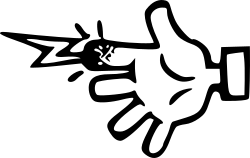
\includegraphics[width=2cm]{sensation}};

\draw (-5.4,-2.6) node [left] {\SI{10}{\milli\ampere}};
\draw [->] (-5.2,-2.6) -- (-4.5,-2.6);
\draw (-4.2,-2.6) node [anchor=mid west, text width=7cm] {Seuil de non lâcher, paralysie musculaire};
\draw (3.2,-2.6) node [anchor=west] {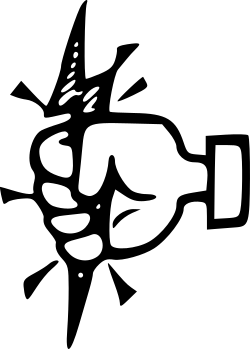
\includegraphics[width=1.5cm]{tetanisation}};

\draw (-5.4,-1.8) node [left] {\SI{30}{\milli\ampere}};
\draw [->] (-5.2,-1.8) -- (-4.5,-1.8);
\draw (-4.2,-1.8) node [anchor=mid west, text width=7cm] {Seuil de paralysie respiratoire};
\draw (7,-1.8) node [anchor=east] {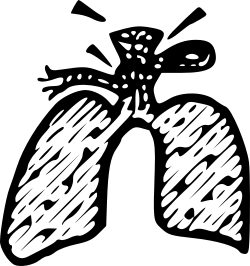
\includegraphics[width=1.5cm]{paralysie_poumon}};

\draw (-5.4,0.7) node [left] {\SI{75}{\milli\ampere}};
\draw [->] (-5.2,0.7) -- (-4.5,0.7);
\draw (-4.2,0.7) node [anchor=mid west, text width=7cm] {Seuil de fibriliation ventriculaire};
\draw (5.1,0.7) node {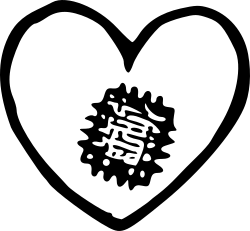
\includegraphics[width=1.5cm]{fibrillation}};

\draw (-5.4,3.1) node [left] {\SI{1}{\ampere}};
\draw [->] (-5.2,3.1) -- (-4.5,3.1);
\draw (-4.2,3.1) node [anchor=mid west, text width=7cm] {Arrêt du coeur};
\draw (5.2,3.1) node {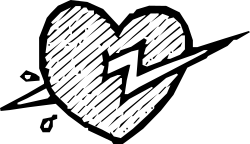
\includegraphics[width=2.4cm]{arret_cardiaque}};

\end{tikzpicture}
\end{figure}

%\end{document}

\subsubsection{Cas particuliers}

Pour le courant alternatifs d'une fréquence supérieures à \SI{100}{\hertz} :

\begin{itemize}
\item Plus la fréquence du courant augmente, plus les risques de fibrillation ventriculaire diminue\,;
\item Plus la fréquence du courant augmente, plus les risques de brûlures augmentent\,;
\item Plus la fréquence du courant augmente, plus l'impédance du corps humain diminue\,;
\item Il est généralement considéré que les conditions de protection contre les contacts indirects sont identiques que ça soit sous une fréquence de \SI{50}{\hertz} (réseau électrique domestique en Europe) où \SI{400}{\hertz} (réseau électrique des bateaux, avions, batmobile\ldots).
\end{itemize}

\subsection{Effet du courant continu}

Les effets du courant continus sont décrits en \autoref{fig:effets_courant_electrique_continu}.

%--------------------------------------
%ELECTROTECHNIQUE - SCHEMA DE LIAISON A LA TERRE
%--------------------------------------

%utiliser les environnement \begin{comment} \end{comment} pour mettre en commentaire le préambule une fois la programmation appelée dans le document maître (!ne pas oublier de mettre en commentaire \end{document}!)

\begin{comment}

\documentclass[a4paper, 11pt, twoside, fleqn]{memoir}

\usepackage{AOCDTF}

%--------------------------------------
%CANEVAS
%--------------------------------------

\newcommand\BoxColor{\ifcase\thechapshift blue!30\or brown!30\or pink!30\or cyan!30\or green!30\or teal!30\or purple!30\or red!30\or olive!30\or orange!30\or lime!30\or gray!\or magenta!30\else yellow!30\fi} %définition de la couleur des marqueurs de chapitre

\newcounter{chapshift} %compteur de chapitre du marqueur de chapitre
\addtocounter{chapshift}{-1}
	
\newif\ifFrame %instruction conditionnelle pour les couleurs des pages
\Frametrue

\pagestyle{plain}

% the main command; the mandatory argument sets the color of the vertical box
\newcommand\ChapFrame{%
\AddEverypageHook{%
\ifFrame
\ifthenelse{\isodd{\value{page}}}
  {\backgroundsetup{contents={%
  \begin{tikzpicture}[overlay,remember picture]
  \node[
  	rounded corners=3pt,
    fill=\BoxColor,
    inner sep=0pt,
    rectangle,
    text width=1.5cm,
    text height=5.5cm,
    align=center,
    anchor=north west
  ] 
  at ($ (current page.north west) + (-0cm,-2*\thechapshift cm) $) %nombre négatif = espacement des marqueurs entre les différents chapitres (à régler en fin de rédaction) (4.5cm vaut un espacement équivalement à la hauteur du marqueur, une page peut en contenir 6 avec cet espacement-la mais il est le plus équilibré)
    {\rotatebox{90}{\hspace*{.5cm}%
      \parbox[c][1.2cm][t]{5cm}{%
        \raggedright\textcolor{black}{\sffamily\textbf{\leftmark}}}}};
  \end{tikzpicture}}}
  }
  {\backgroundsetup{contents={%
  \begin{tikzpicture}[overlay,remember picture]
  \node[
  	rounded corners=3pt,
    fill=\BoxColor,
    inner sep=0pt,
    rectangle,
    text width=1.5cm,
    text height=5.5cm,
    align=center,
    anchor=north east
  ] 
  at ($ (current page.north east) + (-0cm,-2*\thechapshift cm) $) %nombre négatif = espacement des marqueurs entre les différents chapitres (à régler en fin de rédaction) (4.5cm vaut un espacement équivalement à la hauteur du marqueur, une page peut en contenir 6 avec cet espacement-la mais il est le plus équilibré)
    {\rotatebox{90}{\hspace*{.5cm}%
      \parbox[c][1.2cm][t]{5cm}{%
        \raggedright\textcolor{black}{\sffamily\textbf{\leftmark}}}}};
  \end{tikzpicture}}}%
  }
  \BgMaterial%
  \fi%
}%
  \stepcounter{chapshift}
}

\renewcommand\chaptermark[1]{\markboth{\thechapter.~#1}{}} %redéfinition du marqueur de chapitre pour ne contenir que le titre du chapitre %à personnaliser selon le nombre de chapitre dans le cours

%--------------------------------------
%corps du document
%--------------------------------------

\begin{document} %corps du document
	\openleft %début de chapitre à gauche

\end{comment}

\begin{figure}[H]
\centering
\caption{Effets du courant continu sur le corps humain \label{fig:effets_courant_electrique_continu}}
\begin{tikzpicture}
%\DrawGrid{(-7,-2)}{(7,5)} %grille d'aide pour le placement des objets

\draw (-7,4) node [right, minimum width=2cm, text width=1.8cm] {\footnotesize{Intensité de contact $I_c$}};
\draw [->] (-5,-1) -- (-5,4);

\draw (-5.4,0) node [left] {\SI{2}{\milli\ampere}};
\draw [->] (-5.2,0) -- (-4.5,0);
\draw (-4.2,0) node [anchor=mid west, text width=7cm] (A) {Sensation de picotements, de très faible à faible};
\draw (6,0) node [anchor=east] {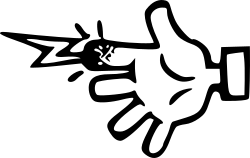
\includegraphics[width=2cm]{sensation}};

\draw (-5.4,1.5) node [left, text width=1cm, align=right] {Non défini};
\draw [->] (-5.2,1.5) -- (-4.5,1.5);
\draw (-4.2,1.5) node [anchor=mid west, text width=7cm] {Seuil de non lâcher, paralysie musculaire};
\draw (3.2,1.5) node [anchor=west] {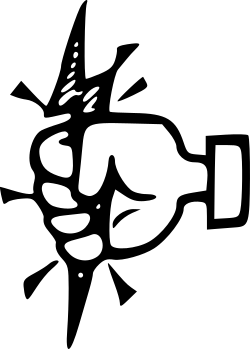
\includegraphics[width=1.5cm]{tetanisation}};

\draw (-5.4,3) node [left] {\SI{130}{\milli\ampere}};
\draw [->] (-5.2,3) -- (-4.5,3);
\draw (-4.2,3) node [anchor=mid west, text width=7cm] {Seuil de fibriliation ventriculaire};
\draw (5.1,3) node {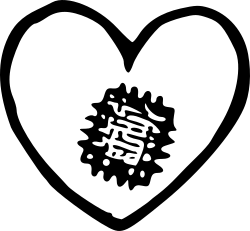
\includegraphics[width=1.5cm]{fibrillation}};

\end{tikzpicture}
\end{figure}

%\end{document}

\begin{itemize}
\item Il est moins difficile de lâcher les parties tenues à la main sous un courant continu\,;
\item Le seuil de fibrillation ventriculaire est plus élevé.
\end{itemize}

\section{Paramètres influençant les risques électriques}

L'intensité de contact $I_c$, la durée de contact $t$, la tension de contact $U_c$ et la résistance du corps humain $R$ sont autant de paramètres à prendre en compte lors de l'évaluation des risques électriques.

\begin{figure}[h]
\caption{Courbe de l'intensité de contact $I_c$ en fonction du temps $t=f(I_c)$\supercite{IEC:60479-2007}\label{graph:intensite_contact_temps}}
\begin{center}
\begin{tikzpicture}

\begin{axis}[
/pgf/number format/.cd, use comma, 1000 sep={\,}, %format numérique européen
axis x line=bottom, axis y line = left,
no markers,
width=\linewidth, height=8cm, %hauteur/largeur
%title={Courbe de l'intensité de contact $I_c$ en fonction du temps $t=f(I_c)$},
grid=major,
enlarge x limits=false, 
xmode=log, xmin=0.1, xmax=6000, xtick={0.1, 0.2, 0.5, 1, 2, 5, 10, 20, 50, 100, 200, 500, 1000, 2000, 5000},
xlabel={Intensité du courant $I_c$ passant dans le corps en \si{\milli\ampere}}, log ticks with fixed point,
ymode=log, ymin=10, ymax=12000, ytick={10, 20, 50, 100, 200, 500, 1000, 2000, 5000, 10000},
ylabel={Durée $t$ du passage du courant en \si{\milli\second}},
]

\path[name path=ha] (0.1,10000) -- (0.5,10000);
\path[name path=la] (0.1,10) -- (0.5,10);
\addplot[YellowGreen, opacity=0.5] fill between[of=la and ha]; %grosse prise de tête pour remplir de couleur entre deux courbes verticales

\addplot [name path=a] (0.5,10) -- (0.5,10000);

\path[name path=ab] (0.5,10) -- (0.5,10000) -- (10.709563224492905,10000);
\addplot [name path=b] table[/pgf/number format/read comma as period]{donnees_courant_duree_b.txt};

\addplot[yellow, opacity=0.5] fill between[of=ab and b];

\addplot [name path=c1, smooth] table[/pgf/number format/read comma as period]{donnees_courant_duree_c1.txt};

\addplot[yellow!75!red, opacity=0.5] fill between[of=b and c1];

\addplot [name path=c2, smooth] table[/pgf/number format/read comma as period]{donnees_courant_duree_c2.txt};

\addplot[yellow!50!red, opacity=0.5] fill between[of= c1 and c2]; %bien inverser le sens d'une des deux listes de données pour que la fonction "fill between" fonctionne correctement

\addplot [name path=c3, smooth] table[/pgf/number format/read comma as period]{donnees_courant_duree_c3.txt};

\addplot[yellow!25!red, opacity=0.5] fill between[of= c2 and c3]; %bien inverser le sens d'une des deux listes de données pour que la fonction "fill between" fonctionne correctement

\path[name path=ec3] (1427.1112552188479, 10) -- (5000,10) -- (5000, 10000);

\addplot[red, opacity=0.5] fill between[of=ec3 and c3];

\end{axis}
\end{tikzpicture}
\end{center}
\end{figure}

\begin{mdframed}
\begin{itemize}
\item[\textcolor{YellowGreen}{\rule{1.5em}{1.2ex}}] Aucune réaction physiologique\,;
\item[\textcolor{yellow}{\rule{1.5em}{1.2ex}}] Aucun effet physiologique dangereux\,;
\item[\textcolor{yellow!75!red}{\rule{1.5em}{1.2ex}}] Aucun dommage corporel. Possibilité de difficultés respiratoires et de contractions musculaires, de troubles réversibles de la formation et de la conduite des impulsions cardiaques (y compris fibrillation des oreillettes et arrêts cardiaques momentanés sans fibrillation ventriculaire ). Phénomènes augmentant proportionnellement avec l'intensité du courant $i_c$ et le temps $t$ d'exposition\,;
\item[\textcolor{yellow!50!red}{\rule{1.5em}{1.2ex}}] Même effets que ceux de la zone \textcolor{yellow!75!red}{\rule{1.5em}{1.2ex}} avec une probabilité de fibrillation ventriculaire augmentant jusqu'à 5\%. Possibilité d'effets physiopathologiques, tels qu'un arrêt cardiaque, un arrêt respiratoire ou des brûlures, augmentant proportionnellement avec l'intensité du courant $i_c$ et le temps $t$ d'exposition\,;
\item[\textcolor{yellow!25!red}{\rule{1.5em}{1.2ex}}] Même effets que ceux de la zone \textcolor{yellow!75!red}{\rule{1.5em}{1.2ex}} avec une probabilité de fibrillation ventriculaire augmentant jusqu'à 50\%. Possibilité d'effets physiopathologiques, tels qu'un arrêt cardiaque, un arrêt respiratoire ou des brûlures, augmentant proportionnellement avec l'intensité du courant $i_c$ et le temps $t$ d'exposition\,;
\item[\textcolor{red}{\rule{1.5em}{1.2ex}}] Même effets que ceux de la zone \textcolor{yellow!75!red}{\rule{1.5em}{1.2ex}} avec une probabilité de fibrillation ventriculaire dépassant 50\%. Possibilité d'effets physiopathologiques, tels qu'un arrêt cardiaque, un arrêt respiratoire ou des brûlures, augmentant proportionnellement avec l'intensité du courant $i_c$ et le temps $t$ d'exposition.
\end{itemize}
\end{mdframed}

Si une personne subit un choc électrique sans en succomber, il s'agit d'une \emph{électrisation}. Si la personne décède suite au choc électrique, il s'agit d'une \emph{électrocution}.

\begin{figure}[H]
\caption{Courbe de la tension de contact $U_c$ en fonction du temps de coupure maximal $t=f(U_c)$\label{graph:tension_contact_temps}}
\begin{center}
\begin{tikzpicture}

\begin{axis}[
/pgf/number format/.cd, use comma, 1000 sep={\,}, %format numérique européen
axis x line=bottom, axis y line = left,
no markers,
width=12cm, height=12cm, %hauteur/largeur
%title={Courbe de la tension de contact $U_c$ en fonction du temps de coupure maximal $t=f(U_c)$},
grid=both,
enlarge x limits=false, 
xmode=log, xmin=10, xmax=600, xtick={10, 20, 30, 50, 100, 200, 300, 500},
xlabel={Tension de contact $U_c$ en \si{\volt}}, log ticks with fixed point,
ymode=log, ymin=0.01, ymax=12, ytick={0.01, 0.02, 0.03, 0.04, 0.05, 1, 0.2, 0.3, 0.4, 0.5, 1, 2, 3, 4, 5, 10},
ylabel={Temps $t$ de coupure maximal en \si\second},
]

\addplot table[/pgf/number format/read comma as period]{donnees_tension_duree_12V.txt};
\addlegendentry{12\si\volt};
\addplot table[/pgf/number format/read comma as period]{donnees_tension_duree_25V.txt};
\addlegendentry{25\si\volt};
\addplot table[/pgf/number format/read comma as period]{donnees_tension_duree_50V.txt};
\addlegendentry{50\si\volt};

\end{axis}
\end{tikzpicture}
\end{center}
\end{figure}

La peau constitue l'isolant contre la pénétration du courant dans le corps humain, et sa résistance électrique varie selon son état de surface et son épaisseur. Pour une peau sèche et fine, on peut estimer que la barrière isolante cède au-delà d'une tension d'environ \SI{50}{\volt}, et le courant pourra dès lors pénétrer de manière plus importante dans le corps humain.\\
En règle générale, on considère la résistance moyenne du corps humain entre \SI{300}{\ohm} et \SI{1000}{\ohm} mais cela peut varier selon les conditions de contact.\supercite{Delahaye2015}

\begin{figure}[H]
\caption{Courbe de la tension de contact \(U_c\) en fonction de la résistance du corps humain \(R=f(U_c)\)\label{graph:tension_contact_resistance}}
\begin{center}
\begin{tikzpicture}

\begin{axis}[
/pgf/number format/.cd, use comma, 1000 sep={\,}, %format numérique européen
axis x line=bottom, axis y line = left,
width=13cm, height=8cm, %hauteur/largeur
%title={Courbe de la tension de contact $U_c$ en fonction de la résistance du corps humain $R=f(U_c)$},
grid=both,
legend cell align={left},
enlarge x limits=false, 
xmin=0, xmax=400, xtick={25, 50, 250, 380},
xlabel={Tension de contact \(U_c\) en \si{\volt}},
ymin=0, ymax=6, ytick={1, 2, 3, 4, 5},
ylabel={Résistance du corps humain \(R\) en \si{\kilo\ohm}},
]

\addplot [smooth, black] table[/pgf/number format/read comma as period]{donnees_tension_resistance_peauseche.txt};
\addlegendentry{Peau sèche};
\addplot [smooth, brown] table[/pgf/number format/read comma as period]{donnees_tension_resistance_peauhumide.txt};
\addlegendentry{Peau humide};
\addplot [smooth, red] table[/pgf/number format/read comma as period]{donnees_tension_resistance_peaumouillee.txt};
\addlegendentry{Peau mouillée};
\addplot [smooth, blue] table[/pgf/number format/read comma as period]{donnees_tension_resistance_peauimmergee.txt};
\addlegendentry{Peau immergée};
\end{axis}
\end{tikzpicture}
\end{center}
\end{figure}

\section{Nature des contacts}

\subsection{Contact direct}

\begin{definition}{Contact direct}{contact_direct}
Contact des personnes avec les parties actives du matériel électrique (pièces ou conducteurs sous tension). La personne rentre en contact direct avec un élément sous tension suite à une négligence ou un non-respect des consignes de sécurité. Dans ce cas, l'électrocution ou l'électrisation sont la conséquence de cette maladresse ou négligence.
\end{definition}

\subsubsection{Catégories}

%--------------------------------------
%ELECTROTECHNIQUE - SCHEMA DE LIAISON A LA TERRE
%--------------------------------------

%utiliser les environnement \begin{comment} \end{comment} pour mettre en commentaire le préambule une fois la programmation appelée dans le document maître (!ne pas oublier de mettre en commentaire \end{document}!)

\begin{comment}

\documentclass[a4paper, 11pt, twoside, fleqn]{memoir}

\usepackage{AOCDTF}

\marqueurchapitre

%lien d'édition des figures Tikz sur le site mathcha.io (rajouter le lien d'une modification effectuée sur la figure tikz avec le nom du modificateur car il n'y a qu'un lien par compte)

%lien éditeur : https://www.mathcha.io/editor/lOoMmIPztP7txmMKGQfM50q0vsXpBMJdhLl73wM

%--------------------------------------
%corps du document
%--------------------------------------

\begin{document} %corps du document

\end{comment}

\begin{wrapfigure}{R}{0pt} %insertion figure dans texte



% Pattern Info
 
\tikzset{
pattern size/.store in=\mcSize, 
pattern size = 5pt,
pattern thickness/.store in=\mcThickness, 
pattern thickness = 0.3pt,
pattern radius/.store in=\mcRadius, 
pattern radius = 1pt}
\makeatletter
\pgfutil@ifundefined{pgf@pattern@name@_gr4cyw3d3}{
\pgfdeclarepatternformonly[\mcThickness,\mcSize]{_gr4cyw3d3}
{\pgfqpoint{0pt}{0pt}}
{\pgfpoint{\mcSize+\mcThickness}{\mcSize+\mcThickness}}
{\pgfpoint{\mcSize}{\mcSize}}
{
\pgfsetcolor{\tikz@pattern@color}
\pgfsetlinewidth{\mcThickness}
\pgfpathmoveto{\pgfqpoint{0pt}{0pt}}
\pgfpathlineto{\pgfpoint{\mcSize+\mcThickness}{\mcSize+\mcThickness}}
\pgfusepath{stroke}
}}
\makeatother
\tikzset{every picture/.style={line width=0.5pt}} %set default line width to 0.75pt        

\begin{tikzpicture}[x=0.75pt,y=0.75pt,yscale=-0.6,xscale=0.6]
%uncomment if require: \path (0,424); %set diagram left start at 0, and has height of 424

%Shape: Rectangle [id:dp2169284611100818] 
\draw  [dash pattern={on 2.25pt off 2.25pt on 1pt off 2.25pt}] (240,197.5) -- (305,197.5) -- (305,240.5) -- (240,240.5) -- cycle ;
%Straight Lines [id:da5696935272389141] 
\draw    (170.5,77) -- (192.5,75) -- (202.5,75) ;
%Straight Lines [id:da6097078488173727] 
\draw    (172.5,75) -- (162.5,75) ;
%Straight Lines [id:da18875603586464362] 
\draw    (170.5,77) -- (174.5,73) ;
%Straight Lines [id:da9004229753221167] 
\draw    (170.5,73) -- (174.5,77) ;

%Straight Lines [id:da3641005609245841] 
\draw    (170.5,57) -- (192.5,55) -- (202.5,55) ;
%Straight Lines [id:da8401165564336985] 
\draw    (172.5,55) -- (162.5,55) ;
%Straight Lines [id:da9896747717915738] 
\draw    (170.5,57) -- (174.5,53) ;
%Straight Lines [id:da31722047594207703] 
\draw    (170.5,53) -- (174.5,57) ;

%Straight Lines [id:da12425045463157547] 
\draw  [dash pattern={on 4.5pt off 4.5pt}]  (181.5,76) -- (181.5,16) ;
%Straight Lines [id:da5940119215502628] 
\draw    (170.5,37) -- (192.5,35) -- (202.5,35) ;
%Straight Lines [id:da2764915022501593] 
\draw    (172.5,35) -- (162.5,35) ;
%Straight Lines [id:da9480245146495652] 
\draw    (170.5,37) -- (174.5,33) ;
%Straight Lines [id:da07417623880545265] 
\draw    (170.5,33) -- (174.5,37) ;

%Straight Lines [id:da8152171343561685] 
\draw    (170.5,17) -- (192.5,15) -- (202.5,15) ;
%Straight Lines [id:da130426482928093] 
\draw    (172.5,15) -- (162.5,15) ;
%Straight Lines [id:da9683813184952329] 
\draw    (170.5,17) -- (174.5,13) ;
%Straight Lines [id:da5321347018666981] 
\draw    (170.5,13) -- (174.5,17) ;


%Straight Lines [id:da7851551246424144] 
\draw    (120,35) -- (162.5,35) ;
%Straight Lines [id:da9606119610661946] 
\draw [color={rgb, 255:red, 139; green, 87; blue, 42 }  ,draw opacity=1 ]   (112.5,15) -- (162.5,15) ;
%Straight Lines [id:da7714909270793904] 
\draw [color={rgb, 255:red, 155; green, 155; blue, 155 }  ,draw opacity=1 ]   (112.5,55) -- (162.5,55) ;
%Straight Lines [id:da6004957425449499] 
\draw [color={rgb, 255:red, 74; green, 144; blue, 226 }  ,draw opacity=1 ]   (87.5,75) -- (162.5,75) ;
%Straight Lines [id:da33029833675036346] 
\draw [color={rgb, 255:red, 248; green, 231; blue, 28 }  ,draw opacity=1 ]   (95.5,35) -- (87.5,65) -- (87.5,265) ;
%Straight Lines [id:da8651297882096667] 
\draw [color={rgb, 255:red, 126; green, 211; blue, 33 }  ,draw opacity=1 ] [dash pattern={on 4.5pt off 4.5pt}]  (95.5,35) -- (87.5,65) -- (87.5,265) ;
%Shape: Circle [id:dp3113483054948739] 
\draw  [fill={rgb, 255:red, 0; green, 0; blue, 0 }  ,fill opacity=1 ] (85,75) .. controls (85,73.62) and (86.12,72.5) .. (87.5,72.5) .. controls (88.88,72.5) and (90,73.62) .. (90,75) .. controls (90,76.38) and (88.88,77.5) .. (87.5,77.5) .. controls (86.12,77.5) and (85,76.38) .. (85,75) -- cycle ;
%Straight Lines [id:da5337274615909295] 
\draw    (202.5,35) -- (332.5,35) ;
%Straight Lines [id:da44799685188646] 
\draw [color={rgb, 255:red, 139; green, 87; blue, 42 }  ,draw opacity=1 ]   (202.5,15) -- (332.5,15) ;
%Straight Lines [id:da1220330851402307] 
\draw [color={rgb, 255:red, 155; green, 155; blue, 155 }  ,draw opacity=1 ]   (202.5,55) -- (332.5,55) ;
%Straight Lines [id:da4257094046245665] 
\draw [color={rgb, 255:red, 74; green, 144; blue, 226 }  ,draw opacity=1 ]   (202.5,75) -- (332.5,75) ;
%Shape: Path Data [id:dp20440693392730014] 
\draw   (112.5,55) .. controls (112.5,56.38) and (111.38,57.5) .. (110,57.5) .. controls (109.29,57.5) and (108.65,57.2) .. (108.19,56.72) .. controls (102.81,61.85) and (95.52,65) .. (87.5,65) .. controls (70.93,65) and (57.5,51.57) .. (57.5,35) .. controls (57.5,18.43) and (70.93,5) .. (87.5,5) .. controls (95.52,5) and (102.81,8.15) .. (108.19,13.28) .. controls (108.65,12.8) and (109.29,12.5) .. (110,12.5) .. controls (111.38,12.5) and (112.5,13.62) .. (112.5,15) .. controls (112.5,15.82) and (112.11,16.54) .. (111.5,17) .. controls (114.8,21.39) and (116.92,26.71) .. (117.4,32.5) .. controls (117.43,32.5) and (117.47,32.5) .. (117.5,32.5) .. controls (118.88,32.5) and (120,33.62) .. (120,35) .. controls (120,36.38) and (118.88,37.5) .. (117.5,37.5) .. controls (117.47,37.5) and (117.43,37.5) .. (117.4,37.5) .. controls (116.92,43.29) and (114.8,48.61) .. (111.5,53) .. controls (112.11,53.46) and (112.5,54.18) .. (112.5,55) -- cycle ;
%Shape: Circle [id:dp5006247847599828] 
\draw   (17.5,35) .. controls (17.5,18.43) and (30.93,5) .. (47.5,5) .. controls (64.07,5) and (77.5,18.43) .. (77.5,35) .. controls (77.5,51.57) and (64.07,65) .. (47.5,65) .. controls (30.93,65) and (17.5,51.57) .. (17.5,35) -- cycle ;
%Shape: Triangle [id:dp6537944472266815] 
\draw   (40,25) -- (30,42.5) -- (50,42.5) -- cycle ;
%Shape: Star [id:dp2613906333324145] 
\draw   (106.75,35) -- (95.5,35) -- (89.88,44.81) -- (95.5,35) -- (89.88,25.19) -- (95.5,35) -- cycle ;
%Shape: Circle [id:dp7131699216499533] 
\draw   (107.5,15) .. controls (107.5,13.62) and (108.62,12.5) .. (110,12.5) .. controls (111.38,12.5) and (112.5,13.62) .. (112.5,15) .. controls (112.5,16.38) and (111.38,17.5) .. (110,17.5) .. controls (108.62,17.5) and (107.5,16.38) .. (107.5,15) -- cycle ;
%Shape: Circle [id:dp052151776417079354] 
\draw   (114.9,35) .. controls (114.9,33.62) and (116.02,32.5) .. (117.4,32.5) .. controls (118.78,32.5) and (119.9,33.62) .. (119.9,35) .. controls (119.9,36.38) and (118.78,37.5) .. (117.4,37.5) .. controls (116.02,37.5) and (114.9,36.38) .. (114.9,35) -- cycle ;
%Shape: Circle [id:dp5618146970792355] 
\draw   (107.5,55) .. controls (107.5,53.62) and (108.62,52.5) .. (110,52.5) .. controls (111.38,52.5) and (112.5,53.62) .. (112.5,55) .. controls (112.5,56.38) and (111.38,57.5) .. (110,57.5) .. controls (108.62,57.5) and (107.5,56.38) .. (107.5,55) -- cycle ;

%Shape: Circle [id:dp1390619762430202] 
\draw  [fill={rgb, 255:red, 0; green, 0; blue, 0 }  ,fill opacity=1 ] (250,15) .. controls (250,13.62) and (251.12,12.5) .. (252.5,12.5) .. controls (253.88,12.5) and (255,13.62) .. (255,15) .. controls (255,16.38) and (253.88,17.5) .. (252.5,17.5) .. controls (251.12,17.5) and (250,16.38) .. (250,15) -- cycle ;
%Shape: Circle [id:dp8146103595826814] 
\draw  [fill={rgb, 255:red, 0; green, 0; blue, 0 }  ,fill opacity=1 ] (270,75) .. controls (270,73.62) and (271.12,72.5) .. (272.5,72.5) .. controls (273.88,72.5) and (275,73.62) .. (275,75) .. controls (275,76.38) and (273.88,77.5) .. (272.5,77.5) .. controls (271.12,77.5) and (270,76.38) .. (270,75) -- cycle ;
%Straight Lines [id:da6885538392628449] 
\draw    (45,242.5) -- (332.5,242.5) ;
%Shape: Rectangle [id:dp9769357556067967] 
\draw  [draw opacity=0][pattern=_gr4cyw3d3,pattern size=6pt,pattern thickness=0.75pt,pattern radius=0pt, pattern color={rgb, 255:red, 0; green, 0; blue, 0}][line width=0.75]  (45,242.5) -- (332.5,242.5) -- (332.5,257.5) -- (45,257.5) -- cycle ;
%Straight Lines [id:da4914891608419114] 
\draw    (87.5,265) -- (87.5,280) ;
%Straight Lines [id:da4130239728468731] 
\draw    (77.5,280) -- (97.5,280) ;
%Straight Lines [id:da6994295900366564] 
\draw    (80,285) -- (95,285) ;
%Straight Lines [id:da8581097227322196] 
\draw    (82.5,290) -- (92.5,290) ;

%Straight Lines [id:da7479204467796963] 
\draw    (287.5,212.5) -- (292.5,212.5) ;
%Shape: Rectangle [id:dp9326988183780455] 
\draw   (257.5,207.5) -- (287.5,207.5) -- (287.5,217.5) -- (257.5,217.5) -- cycle ;
%Straight Lines [id:da6189064136247362] 
\draw    (252.5,212.5) -- (257.5,212.5) ;

%Straight Lines [id:da11351623748674167] 
\draw [color={rgb, 255:red, 139; green, 87; blue, 42 }  ,draw opacity=1 ]   (252.5,210) -- (252.5,17.5) ;
%Straight Lines [id:da9349245679018577] 
\draw [color={rgb, 255:red, 74; green, 144; blue, 226 }  ,draw opacity=1 ]   (292.5,210) -- (292.5,155) -- (272.5,155) -- (272.5,77.5) ;
%Straight Lines [id:da8151373432214233] 
\draw    (209.07,239.53) -- (199.07,242.03) -- (206.57,214.53) -- (204.07,187.03) -- (193.53,143.6) -- (221.57,144.53) -- (204.07,187.03) -- (224.07,202.03) -- (234.07,229.53) -- (238.57,217.53) ;
%Straight Lines [id:da7007304063321129] 
\draw    (235,75) -- (240,87.5) -- (232.5,122.5) -- (191.96,144.07) -- (220,145) -- (232.5,167.5) -- (245,175) -- (252.5,167.5) ;
%Straight Lines [id:da32616186175416606] 
\draw    (203.64,133.68) -- (207.55,144.07) ;
%Shape: Ellipse [id:dp3314169529451746] 
\draw   (190,120.04) .. controls (190,112.5) and (196.11,106.4) .. (203.64,106.4) .. controls (211.17,106.4) and (217.28,112.5) .. (217.28,120.04) .. controls (217.28,127.57) and (211.17,133.68) .. (203.64,133.68) .. controls (196.11,133.68) and (190,127.57) .. (190,120.04) -- cycle ;
%Shape: Arc [id:dp10949273996813036] 
\draw  [draw opacity=0][fill={rgb, 255:red, 0; green, 0; blue, 0 }  ,fill opacity=1 ] (216.88,111.86) .. controls (214.27,107.8) and (209.79,105.12) .. (204.71,105.12) .. controls (196.67,105.12) and (190.15,111.81) .. (190.15,120.06) .. controls (190.15,122.2) and (190.58,124.23) .. (191.37,126.07) -- (204.71,120.06) -- cycle ; \draw   (216.88,111.86) .. controls (214.27,107.8) and (209.79,105.12) .. (204.71,105.12) .. controls (196.67,105.12) and (190.15,111.81) .. (190.15,120.06) .. controls (190.15,122.2) and (190.58,124.23) .. (191.37,126.07) ;
%Shape: Boxed Line [id:dp41496467515533] 
\draw    (227.65,103.32) -- (191.37,126.07) ;

%Straight Lines [id:da9825870173077352] 
\draw [color={rgb, 255:red, 208; green, 2; blue, 27 }  ,draw opacity=1 ] [dash pattern={on 0.75pt off 0.75pt}]  (95.5,35) .. controls (96.68,37.04) and (96.25,38.65) .. (94.21,39.83) .. controls (92.17,41.01) and (91.74,42.62) .. (92.92,44.66) .. controls (94.11,46.7) and (93.68,48.31) .. (91.64,49.49) .. controls (89.6,50.67) and (89.17,52.28) .. (90.35,54.32) .. controls (91.53,56.36) and (91.1,57.97) .. (89.06,59.16) .. controls (87.02,60.34) and (86.59,61.95) .. (87.77,63.99) -- (87.5,65) -- (87.5,65) .. controls (89.17,66.67) and (89.17,68.33) .. (87.5,70) .. controls (85.83,71.67) and (85.83,73.33) .. (87.5,75) -- (87.5,75) .. controls (89.17,73.33) and (90.83,73.33) .. (92.5,75) .. controls (94.17,76.67) and (95.83,76.67) .. (97.5,75) .. controls (99.17,73.33) and (100.83,73.33) .. (102.5,75) .. controls (104.17,76.67) and (105.83,76.67) .. (107.5,75) .. controls (109.17,73.33) and (110.83,73.33) .. (112.5,75) .. controls (114.17,76.67) and (115.83,76.67) .. (117.5,75) .. controls (119.17,73.33) and (120.83,73.33) .. (122.5,75) .. controls (124.17,76.67) and (125.83,76.67) .. (127.5,75) .. controls (129.17,73.33) and (130.83,73.33) .. (132.5,75) .. controls (134.17,76.67) and (135.83,76.67) .. (137.5,75) .. controls (139.17,73.33) and (140.83,73.33) .. (142.5,75) .. controls (144.17,76.67) and (145.83,76.67) .. (147.5,75) .. controls (149.17,73.33) and (150.83,73.33) .. (152.5,75) .. controls (154.17,76.67) and (155.83,76.67) .. (157.5,75) .. controls (159.17,73.33) and (160.83,73.33) .. (162.5,75) .. controls (164.17,76.67) and (165.83,76.67) .. (167.5,75) .. controls (169.17,73.33) and (170.83,73.33) .. (172.5,75) .. controls (174.17,76.67) and (175.83,76.67) .. (177.5,75) .. controls (179.17,73.33) and (180.83,73.33) .. (182.5,75) .. controls (184.17,76.67) and (185.83,76.67) .. (187.5,75) .. controls (189.17,73.33) and (190.83,73.33) .. (192.5,75) .. controls (194.17,76.67) and (195.83,76.67) .. (197.5,75) .. controls (199.17,73.33) and (200.83,73.33) .. (202.5,75) .. controls (204.17,76.67) and (205.83,76.67) .. (207.5,75) .. controls (209.17,73.33) and (210.83,73.33) .. (212.5,75) .. controls (214.17,76.67) and (215.83,76.67) .. (217.5,75) .. controls (219.17,73.33) and (220.83,73.33) .. (222.5,75) .. controls (224.17,76.67) and (225.83,76.67) .. (227.5,75) .. controls (229.17,73.33) and (230.83,73.33) .. (232.5,75) -- (235,75) -- (235,75) .. controls (237.17,75.93) and (237.79,77.47) .. (236.86,79.64) .. controls (235.93,81.81) and (236.54,83.35) .. (238.71,84.28) -- (240,87.5) -- (240,87.5) .. controls (241.28,89.48) and (240.93,91.11) .. (238.95,92.39) .. controls (236.97,93.67) and (236.62,95.3) .. (237.9,97.28) .. controls (239.19,99.26) and (238.84,100.89) .. (236.86,102.17) .. controls (234.88,103.45) and (234.53,105.08) .. (235.81,107.06) .. controls (237.09,109.04) and (236.74,110.67) .. (234.76,111.95) .. controls (232.78,113.22) and (232.43,114.85) .. (233.71,116.83) .. controls (235,118.81) and (234.65,120.44) .. (232.67,121.72) -- (232.5,122.5) -- (232.5,122.5) .. controls (231.81,124.75) and (230.34,125.54) .. (228.09,124.85) .. controls (225.84,124.16) and (224.36,124.95) .. (223.67,127.2) .. controls (222.98,129.45) and (221.51,130.24) .. (219.26,129.55) .. controls (217.01,128.86) and (215.53,129.64) .. (214.84,131.89) .. controls (214.15,134.14) and (212.68,134.93) .. (210.43,134.24) .. controls (208.18,133.55) and (206.71,134.34) .. (206.02,136.59) .. controls (205.33,138.84) and (203.85,139.63) .. (201.6,138.94) .. controls (199.35,138.25) and (197.88,139.04) .. (197.19,141.29) .. controls (196.5,143.54) and (195.02,144.33) .. (192.77,143.64) -- (191.96,144.07) -- (191.96,144.07) .. controls (193.68,142.46) and (195.35,142.51) .. (196.96,144.23) .. controls (198.57,145.95) and (200.24,146.01) .. (201.96,144.4) .. controls (203.68,142.79) and (205.34,142.85) .. (206.95,144.57) .. controls (208.56,146.29) and (210.23,146.34) .. (211.95,144.73) .. controls (213.67,143.12) and (215.34,143.18) .. (216.95,144.9) -- (220,145) -- (220,145) .. controls (222.27,145.65) and (223.08,147.1) .. (222.43,149.37) .. controls (221.78,151.64) and (222.59,153.09) .. (224.86,153.74) .. controls (227.13,154.39) and (227.93,155.84) .. (227.28,158.11) .. controls (226.63,160.38) and (227.44,161.83) .. (229.71,162.48) .. controls (231.98,163.13) and (232.79,164.58) .. (232.14,166.85) -- (232.5,167.5) -- (232.5,167.5) .. controls (234.79,166.93) and (236.22,167.78) .. (236.79,170.07) .. controls (237.36,172.36) and (238.78,173.21) .. (241.07,172.64) -- (245,175) -- (245,175) .. controls (245,172.64) and (246.18,171.46) .. (248.54,171.46) .. controls (250.89,171.46) and (252.07,170.28) .. (252.07,167.93) -- (252.5,167.5) -- (252.5,167.5) .. controls (250.83,165.83) and (250.83,164.17) .. (252.5,162.5) .. controls (254.17,160.83) and (254.17,159.17) .. (252.5,157.5) .. controls (250.83,155.83) and (250.83,154.17) .. (252.5,152.5) .. controls (254.17,150.83) and (254.17,149.17) .. (252.5,147.5) .. controls (250.83,145.83) and (250.83,144.17) .. (252.5,142.5) .. controls (254.17,140.83) and (254.17,139.17) .. (252.5,137.5) .. controls (250.83,135.83) and (250.83,134.17) .. (252.5,132.5) .. controls (254.17,130.83) and (254.17,129.17) .. (252.5,127.5) .. controls (250.83,125.83) and (250.83,124.17) .. (252.5,122.5) .. controls (254.17,120.83) and (254.17,119.17) .. (252.5,117.5) .. controls (250.83,115.83) and (250.83,114.17) .. (252.5,112.5) .. controls (254.17,110.83) and (254.17,109.17) .. (252.5,107.5) .. controls (250.83,105.83) and (250.83,104.17) .. (252.5,102.5) .. controls (254.17,100.83) and (254.17,99.17) .. (252.5,97.5) .. controls (250.83,95.83) and (250.83,94.17) .. (252.5,92.5) .. controls (254.17,90.83) and (254.17,89.17) .. (252.5,87.5) .. controls (250.83,85.83) and (250.83,84.17) .. (252.5,82.5) .. controls (254.17,80.83) and (254.17,79.17) .. (252.5,77.5) .. controls (250.83,75.83) and (250.83,74.17) .. (252.5,72.5) .. controls (254.17,70.83) and (254.17,69.17) .. (252.5,67.5) .. controls (250.83,65.83) and (250.83,64.17) .. (252.5,62.5) .. controls (254.17,60.83) and (254.17,59.17) .. (252.5,57.5) .. controls (250.83,55.83) and (250.83,54.17) .. (252.5,52.5) .. controls (254.17,50.83) and (254.17,49.17) .. (252.5,47.5) .. controls (250.83,45.83) and (250.83,44.17) .. (252.5,42.5) .. controls (254.17,40.83) and (254.17,39.17) .. (252.5,37.5) .. controls (250.83,35.83) and (250.83,34.17) .. (252.5,32.5) .. controls (254.17,30.83) and (254.17,29.17) .. (252.5,27.5) .. controls (250.83,25.83) and (250.83,24.17) .. (252.5,22.5) .. controls (254.17,20.83) and (254.17,19.17) .. (252.5,17.5) -- (252.5,15) -- (252.5,15) .. controls (250.83,16.67) and (249.17,16.67) .. (247.5,15) .. controls (245.83,13.33) and (244.17,13.33) .. (242.5,15) .. controls (240.83,16.67) and (239.17,16.67) .. (237.5,15) .. controls (235.83,13.33) and (234.17,13.33) .. (232.5,15) .. controls (230.83,16.67) and (229.17,16.67) .. (227.5,15) .. controls (225.83,13.33) and (224.17,13.33) .. (222.5,15) .. controls (220.83,16.67) and (219.17,16.67) .. (217.5,15) .. controls (215.83,13.33) and (214.17,13.33) .. (212.5,15) .. controls (210.83,16.67) and (209.17,16.67) .. (207.5,15) .. controls (205.83,13.33) and (204.17,13.33) .. (202.5,15) .. controls (200.83,16.67) and (199.17,16.67) .. (197.5,15) .. controls (195.83,13.33) and (194.17,13.33) .. (192.5,15) .. controls (190.83,16.67) and (189.17,16.67) .. (187.5,15) .. controls (185.83,13.33) and (184.17,13.33) .. (182.5,15) .. controls (180.83,16.67) and (179.17,16.67) .. (177.5,15) .. controls (175.83,13.33) and (174.17,13.33) .. (172.5,15) .. controls (170.83,16.67) and (169.17,16.67) .. (167.5,15) .. controls (165.83,13.33) and (164.17,13.33) .. (162.5,15) .. controls (160.83,16.67) and (159.17,16.67) .. (157.5,15) .. controls (155.83,13.33) and (154.17,13.33) .. (152.5,15) .. controls (150.83,16.67) and (149.17,16.67) .. (147.5,15) .. controls (145.83,13.33) and (144.17,13.33) .. (142.5,15) .. controls (140.83,16.67) and (139.17,16.67) .. (137.5,15) .. controls (135.83,13.33) and (134.17,13.33) .. (132.5,15) .. controls (130.83,16.67) and (129.17,16.67) .. (127.5,15) .. controls (125.83,13.33) and (124.17,13.33) .. (122.5,15) .. controls (120.83,16.67) and (119.17,16.67) .. (117.5,15) .. controls (115.83,13.33) and (114.17,13.33) .. (112.5,15) -- (110,15) -- (110,15) ;
%Shape: Boxed Line [id:dp46367613794770235] 
\draw    (264.13,137.15) -- (252.3,154.04) -- (264.33,150.61) -- (254.22,165.04) ;
\draw [shift={(252.5,167.5)}, rotate = 305.01] [fill={rgb, 255:red, 0; green, 0; blue, 0 }  ][line width=0.08]  [draw opacity=0] (5.36,-2.57) -- (0,0) -- (5.36,2.57) -- cycle    ;
%Straight Lines [id:da7937546897023091] 
\draw    (235,42.5) -- (230,62.5) -- (240,55) -- (235.73,72.09) ;
\draw [shift={(235,75)}, rotate = 284.04] [fill={rgb, 255:red, 0; green, 0; blue, 0 }  ][line width=0.08]  [draw opacity=0] (5.36,-2.57) -- (0,0) -- (5.36,2.57) -- cycle    ;
%Shape: Circle [id:dp1596792694174739] 
\draw  [fill={rgb, 255:red, 255; green, 255; blue, 255 }  ,fill opacity=1 ] (250,212.5) .. controls (250,211.12) and (251.12,210) .. (252.5,210) .. controls (253.88,210) and (255,211.12) .. (255,212.5) .. controls (255,213.88) and (253.88,215) .. (252.5,215) .. controls (251.12,215) and (250,213.88) .. (250,212.5) -- cycle ;
%Shape: Circle [id:dp6844783325646259] 
\draw  [fill={rgb, 255:red, 255; green, 255; blue, 255 }  ,fill opacity=1 ] (290,212.5) .. controls (290,211.12) and (291.12,210) .. (292.5,210) .. controls (293.88,210) and (295,211.12) .. (295,212.5) .. controls (295,213.88) and (293.88,215) .. (292.5,215) .. controls (291.12,215) and (290,213.88) .. (290,212.5) -- cycle ;




\end{tikzpicture}

\end{wrapfigure}

%\end{document}


\begin{comment}


\begin{circuitikz}[circuit ee IEC]
%\DrawGrid{(-1,-5)}{(7,3)} %grille d'aide pour le placement des objets

\fill [gray!50] (-1,-3.5) -- (5,-3.5) -- (5,-3.7) -- (-1,-3.7) -- cycle;
\draw [thick] (-1,-3.5) -- (5,-3.5);

\node (T1) [oosourcetransshape,prim=delta,sec=wye] at (0,0) {};
\draw [brown] (-1,0.3) to (-0.5,0.3) to node {} (T1.prim1);
\draw [black] (-1,0) to (-0.5,0) to node {} (T1.prim2);
\draw [gray] (-1,-0.3) to (-0.5,-0.3) to node {} (T1.prim3);
\draw [brown] (5,0.3) to (1,0.3) to (0.5,0.3) to node {} (T1.sec1);
\draw [black] (5,0.1) to (1,0.1) to (0.5,0.1) to node {} (T1.sec2);
\draw [gray] (5,-0.1) to (1,-0.1) to (0.5,-0.1) to node {} (T1.sec3);
\draw [blue] (5,-0.3) to (1,-0.3) to (0.5,-0.3) to node {} (T1.sec4);
\node (G) [tlground] at (0,-3.9) {};
\draw [green!] (G) to (0,-0.4) to node {} (T1.sec4) ; 
\draw [dashed, yellow!] (G) to (0,-0.4) to node {} (T1.sec4) ;
\node (G) [tlground] at (0,-3.9) {};
\node (T1) [oosourcetransshape,prim=delta,sec=wye] at (0,0) {};

\node (L) [bulb] at (1.7,-2.5) {};
\draw [brown] (1.7,0.3) to node {} (L);
\draw [blue] (1.3,-0.3) to (1.3,-3) to (1.7,-3) to node {} (L);

\draw (1.7,0.3) node[circ, scale=0.5]{};
\draw (1.3,-0.3) node[circ, scale=0.5]{};



\draw (3,-1.5) -- (3.3,-2.5) -- (3.6,-1.5) ; %tronc
\draw (3.3,-1.5) -- (3.3, -1.3); %cou
\draw (3.3,-1) circle [radius=0.3cm]; %tête
\draw (1.7,-1.7) -- (1.9,-1.7) -- (2.4,-1.4)  -- (3,-1.5) -- (3.6,-1.5) -- (4,-1) -- (4,-0.4) -- (3.8,-0.3); %bras
\draw (2.4,-2.8) -- (2.5,-3) -- (2.8, -2.7) -- (3.3,-2.5) -- (3.6,-3.4) -- (3.4,-3.5); %jambes
\filldraw ([shift=(-10:0.3cm)]3.3,-1) arc (-10:150:0.3cm); %casquette
\draw (3.04,-0.84) -- ++ (140:0.3cm); 

\fill [yellow!, decoration=lightning bolt, decorate] (1.7,-1.7) -- ++ (0.5,0.8); %éclairs
\fill [yellow!, decoration=lightning bolt, decorate] (3.8,-0.3) -- ++ (0.5,0.8); %éclairs
\path [postaction={on each segment={mid arrow=red}}] (1.7,-1.7) -- (1.9,-1.7) -- (2.4,-1.4)  -- (3,-1.5) -- (3.6,-1.5) -- (4,-1) -- (4,-0.4) -- (3.8,-0.3);; 

\end{circuitikz}

\end{comment}




\paragraph{Contact entre deux phases ou la phase et le neutre} 
Contact le moins fréquent mais le plus dangereux car la résistance pied/sol n'intervient pas. La personne qui touche les deux est alors soumise à la tension simple \(U_0\) ou composée \(U\) du réseau. La résistance globale du corps devient alors très faible et le courant en est d'autant plus élevé.\\ Dans ce cas, le corps humain se comporte comme un récepteur et aucun appareil de coupure ne peut détecter ce contact comme provoquant un défaut, seule une intervention externe pourra couper le courant.\\

\begin{exemple}{Contact direct phase/neutre}{}
Si la personne est soumise à une tension de contact \(U_c\) de \SI{230}{\volt} et que l'on estime la résistance résultante \(R\) des résistance main/fil + résistance des bras à environ \SI{1,5}{\kilo\ohm}, on peut calculer l'intensité du courant traversant le corps comme suit :

\begin{align*}
I 	&= \frac{U_c}{R} \\
	&= \frac{230}{1500} \\
	&= \SI{150}{\milli\ampere}
\end{align*}

En se référençant au tableau \superref{graph:intensite_contact_temps}, on peut constater que le temps de réaction de coupure (venant d'une intervention externe) doit être très court. Effectivement, après une seconde, le risque de fibrillation ventriculaire dépasse déjà les 50\%, ce qui augmente sensiblement le risque d'arrêt cardiaque.
\end{exemple}

%--------------------------------------
%ELECTROTECHNIQUE - SCHEMA DE LIAISON A LA TERRE
%--------------------------------------

%utiliser les environnement \begin{comment} \end{comment} pour mettre en commentaire le préambule une fois la programmation appelée dans le document maître (!ne pas oublier de mettre en commentaire \end{document}!)

\begin{comment}

\documentclass[a4paper, 11pt, twoside, fleqn]{memoir}

\usepackage{AOCDTF}

\marqueurchapitre

%lien éditeur : https://www.mathcha.io/editor/d2ZzzhP8twWsr4JDjKcPLrw6KCe4Y7GKhzE68mv

%--------------------------------------
%corps du document
%--------------------------------------

\begin{document} %corps du document
	\openleft %début de chapitre à gauche

\end{comment}

\begin{wrapfigure}{R}{0pt} %insertion figure dans texte


% Pattern Info
 
\tikzset{
pattern size/.store in=\mcSize, 
pattern size = 5pt,
pattern thickness/.store in=\mcThickness, 
pattern thickness = 0.3pt,
pattern radius/.store in=\mcRadius, 
pattern radius = 1pt}
\makeatletter
\pgfutil@ifundefined{pgf@pattern@name@_nwdeo5h1b}{
\pgfdeclarepatternformonly[\mcThickness,\mcSize]{_nwdeo5h1b}
{\pgfqpoint{0pt}{0pt}}
{\pgfpoint{\mcSize+\mcThickness}{\mcSize+\mcThickness}}
{\pgfpoint{\mcSize}{\mcSize}}
{
\pgfsetcolor{\tikz@pattern@color}
\pgfsetlinewidth{\mcThickness}
\pgfpathmoveto{\pgfqpoint{0pt}{0pt}}
\pgfpathlineto{\pgfpoint{\mcSize+\mcThickness}{\mcSize+\mcThickness}}
\pgfusepath{stroke}
}}
\makeatother
\tikzset{every picture/.style={line width=0.5pt}} %set default line width to 0.75pt        

\begin{tikzpicture}[x=0.75pt,y=0.75pt,yscale=-0.6,xscale=0.6]
%uncomment if require: \path (0,424); %set diagram left start at 0, and has height of 424

%Shape: Rectangle [id:dp15718458701164983] 
\draw  [dash pattern={on 2.25pt off 2.25pt on 1pt off 2.25pt}] (240,197.5) -- (305,197.5) -- (305,240.5) -- (240,240.5) -- cycle ;
%Straight Lines [id:da5819627805434486] 
\draw    (170.5,77) -- (192.5,75) -- (202.5,75) ;
%Straight Lines [id:da8932065287705061] 
\draw    (172.5,75) -- (162.5,75) ;
%Straight Lines [id:da0074898535006566735] 
\draw    (170.5,77) -- (174.5,73) ;
%Straight Lines [id:da4628981634403191] 
\draw    (170.5,73) -- (174.5,77) ;

%Straight Lines [id:da07833217387555325] 
\draw    (170.5,57) -- (192.5,55) -- (202.5,55) ;
%Straight Lines [id:da21193916411264146] 
\draw    (172.5,55) -- (162.5,55) ;
%Straight Lines [id:da3942014650362937] 
\draw    (170.5,57) -- (174.5,53) ;
%Straight Lines [id:da22890303027954362] 
\draw    (170.5,53) -- (174.5,57) ;

%Straight Lines [id:da8934902011202547] 
\draw  [dash pattern={on 4.5pt off 4.5pt}]  (181.5,76) -- (181.5,16) ;
%Straight Lines [id:da5863396976462423] 
\draw    (170.5,37) -- (192.5,35) -- (202.5,35) ;
%Straight Lines [id:da1593957266571825] 
\draw    (172.5,35) -- (162.5,35) ;
%Straight Lines [id:da9877754703831522] 
\draw    (170.5,37) -- (174.5,33) ;
%Straight Lines [id:da7330425730211421] 
\draw    (170.5,33) -- (174.5,37) ;

%Straight Lines [id:da8701094586336697] 
\draw    (170.5,17) -- (192.5,15) -- (202.5,15) ;
%Straight Lines [id:da08604015821428634] 
\draw    (172.5,15) -- (162.5,15) ;
%Straight Lines [id:da8630577370516217] 
\draw    (170.5,17) -- (174.5,13) ;
%Straight Lines [id:da9623873737598048] 
\draw    (170.5,13) -- (174.5,17) ;


%Straight Lines [id:da008625218884382724] 
\draw    (120,35) -- (162.5,35) ;
%Straight Lines [id:da22628263129456871] 
\draw [color={rgb, 255:red, 139; green, 87; blue, 42 }  ,draw opacity=1 ]   (112.5,15) -- (162.5,15) ;
%Straight Lines [id:da25798344669876005] 
\draw [color={rgb, 255:red, 155; green, 155; blue, 155 }  ,draw opacity=1 ]   (112.5,55) -- (162.5,55) ;
%Straight Lines [id:da27042664843808295] 
\draw [color={rgb, 255:red, 74; green, 144; blue, 226 }  ,draw opacity=1 ]   (87.5,75) -- (162.5,75) ;
%Straight Lines [id:da9940649439482242] 
\draw [color={rgb, 255:red, 248; green, 231; blue, 28 }  ,draw opacity=1 ]   (95.5,35) -- (87.5,65) -- (87.5,265) ;
%Straight Lines [id:da5613771031662728] 
\draw [color={rgb, 255:red, 126; green, 211; blue, 33 }  ,draw opacity=1 ] [dash pattern={on 4.5pt off 4.5pt}]  (95.5,35) -- (87.5,65) -- (87.5,265) ;
%Shape: Circle [id:dp42293753419737434] 
\draw  [fill={rgb, 255:red, 0; green, 0; blue, 0 }  ,fill opacity=1 ] (85,75) .. controls (85,73.62) and (86.12,72.5) .. (87.5,72.5) .. controls (88.88,72.5) and (90,73.62) .. (90,75) .. controls (90,76.38) and (88.88,77.5) .. (87.5,77.5) .. controls (86.12,77.5) and (85,76.38) .. (85,75) -- cycle ;
%Straight Lines [id:da3579360283638311] 
\draw    (202.5,35) -- (332.5,35) ;
%Straight Lines [id:da6741497275385713] 
\draw [color={rgb, 255:red, 139; green, 87; blue, 42 }  ,draw opacity=1 ]   (202.5,15) -- (332.5,15) ;
%Straight Lines [id:da4616399232059213] 
\draw [color={rgb, 255:red, 155; green, 155; blue, 155 }  ,draw opacity=1 ]   (202.5,55) -- (332.5,55) ;
%Straight Lines [id:da49245972642717517] 
\draw [color={rgb, 255:red, 74; green, 144; blue, 226 }  ,draw opacity=1 ]   (202.5,75) -- (332.5,75) ;
%Shape: Path Data [id:dp6620845199778955] 
\draw   (112.5,55) .. controls (112.5,56.38) and (111.38,57.5) .. (110,57.5) .. controls (109.29,57.5) and (108.65,57.2) .. (108.19,56.72) .. controls (102.81,61.85) and (95.52,65) .. (87.5,65) .. controls (70.93,65) and (57.5,51.57) .. (57.5,35) .. controls (57.5,18.43) and (70.93,5) .. (87.5,5) .. controls (95.52,5) and (102.81,8.15) .. (108.19,13.28) .. controls (108.65,12.8) and (109.29,12.5) .. (110,12.5) .. controls (111.38,12.5) and (112.5,13.62) .. (112.5,15) .. controls (112.5,15.82) and (112.11,16.54) .. (111.5,17) .. controls (114.8,21.39) and (116.92,26.71) .. (117.4,32.5) .. controls (117.43,32.5) and (117.47,32.5) .. (117.5,32.5) .. controls (118.88,32.5) and (120,33.62) .. (120,35) .. controls (120,36.38) and (118.88,37.5) .. (117.5,37.5) .. controls (117.47,37.5) and (117.43,37.5) .. (117.4,37.5) .. controls (116.92,43.29) and (114.8,48.61) .. (111.5,53) .. controls (112.11,53.46) and (112.5,54.18) .. (112.5,55) -- cycle ;
%Shape: Circle [id:dp9487272290382273] 
\draw   (17.5,35) .. controls (17.5,18.43) and (30.93,5) .. (47.5,5) .. controls (64.07,5) and (77.5,18.43) .. (77.5,35) .. controls (77.5,51.57) and (64.07,65) .. (47.5,65) .. controls (30.93,65) and (17.5,51.57) .. (17.5,35) -- cycle ;
%Shape: Triangle [id:dp7938424960892552] 
\draw   (40,25) -- (30,42.5) -- (50,42.5) -- cycle ;
%Shape: Star [id:dp49007233964578545] 
\draw   (106.75,35) -- (95.5,35) -- (89.88,44.81) -- (95.5,35) -- (89.88,25.19) -- (95.5,35) -- cycle ;
%Shape: Circle [id:dp15495247495745434] 
\draw   (107.5,15) .. controls (107.5,13.62) and (108.62,12.5) .. (110,12.5) .. controls (111.38,12.5) and (112.5,13.62) .. (112.5,15) .. controls (112.5,16.38) and (111.38,17.5) .. (110,17.5) .. controls (108.62,17.5) and (107.5,16.38) .. (107.5,15) -- cycle ;
%Shape: Circle [id:dp9203062168728426] 
\draw   (114.9,35) .. controls (114.9,33.62) and (116.02,32.5) .. (117.4,32.5) .. controls (118.78,32.5) and (119.9,33.62) .. (119.9,35) .. controls (119.9,36.38) and (118.78,37.5) .. (117.4,37.5) .. controls (116.02,37.5) and (114.9,36.38) .. (114.9,35) -- cycle ;
%Shape: Circle [id:dp4666836922586747] 
\draw   (107.5,55) .. controls (107.5,53.62) and (108.62,52.5) .. (110,52.5) .. controls (111.38,52.5) and (112.5,53.62) .. (112.5,55) .. controls (112.5,56.38) and (111.38,57.5) .. (110,57.5) .. controls (108.62,57.5) and (107.5,56.38) .. (107.5,55) -- cycle ;

%Shape: Circle [id:dp7076438877620288] 
\draw  [fill={rgb, 255:red, 0; green, 0; blue, 0 }  ,fill opacity=1 ] (250,15) .. controls (250,13.62) and (251.12,12.5) .. (252.5,12.5) .. controls (253.88,12.5) and (255,13.62) .. (255,15) .. controls (255,16.38) and (253.88,17.5) .. (252.5,17.5) .. controls (251.12,17.5) and (250,16.38) .. (250,15) -- cycle ;
%Shape: Circle [id:dp8152444678898833] 
\draw  [fill={rgb, 255:red, 0; green, 0; blue, 0 }  ,fill opacity=1 ] (270,75) .. controls (270,73.62) and (271.12,72.5) .. (272.5,72.5) .. controls (273.88,72.5) and (275,73.62) .. (275,75) .. controls (275,76.38) and (273.88,77.5) .. (272.5,77.5) .. controls (271.12,77.5) and (270,76.38) .. (270,75) -- cycle ;
%Shape: Rectangle [id:dp3633744062866603] 
\draw  [draw opacity=0][pattern=_nwdeo5h1b,pattern size=6pt,pattern thickness=0.75pt,pattern radius=0pt, pattern color={rgb, 255:red, 0; green, 0; blue, 0}][line width=0.75]  (45,242.5) -- (332.5,242.5) -- (332.5,257.5) -- (45,257.5) -- cycle ;
%Straight Lines [id:da5268710384268228] 
\draw    (87.5,265) -- (87.5,280) ;
%Straight Lines [id:da32905011254645133] 
\draw    (77.5,280) -- (97.5,280) ;
%Straight Lines [id:da1412531787393071] 
\draw    (80,285) -- (95,285) ;
%Straight Lines [id:da2575017127393042] 
\draw    (82.5,290) -- (92.5,290) ;

%Straight Lines [id:da02413525722256349] 
\draw    (207.5,240) -- (197.5,242.5) -- (205,215) -- (202.5,187.5) -- (191.96,144.07) -- (220,145) -- (202.5,187.5) -- (222.5,202.5) -- (232.5,230) -- (237,218) ;
%Straight Lines [id:da3531360853267902] 
\draw    (155,105) -- (152.5,117.5) -- (167.5,137.5) -- (191.96,144.07) -- (220,145) -- (232.5,167.5) -- (245,175) -- (252.5,167.5) ;
%Straight Lines [id:da8908268923304523] 
\draw    (203.64,133.68) -- (207.55,144.07) ;
%Shape: Ellipse [id:dp5992297332240032] 
\draw   (190,120.04) .. controls (190,112.5) and (196.11,106.4) .. (203.64,106.4) .. controls (211.17,106.4) and (217.28,112.5) .. (217.28,120.04) .. controls (217.28,127.57) and (211.17,133.68) .. (203.64,133.68) .. controls (196.11,133.68) and (190,127.57) .. (190,120.04) -- cycle ;
%Shape: Arc [id:dp676034431482982] 
\draw  [draw opacity=0][fill={rgb, 255:red, 0; green, 0; blue, 0 }  ,fill opacity=1 ] (216.88,111.86) .. controls (214.27,107.8) and (209.79,105.12) .. (204.71,105.12) .. controls (196.67,105.12) and (190.15,111.81) .. (190.15,120.06) .. controls (190.15,122.2) and (190.58,124.23) .. (191.37,126.07) -- (204.71,120.06) -- cycle ; \draw   (216.88,111.86) .. controls (214.27,107.8) and (209.79,105.12) .. (204.71,105.12) .. controls (196.67,105.12) and (190.15,111.81) .. (190.15,120.06) .. controls (190.15,122.2) and (190.58,124.23) .. (191.37,126.07) ;
%Shape: Boxed Line [id:dp7031906239888388] 
\draw    (227.65,103.32) -- (191.37,126.07) ;

%Shape: Boxed Line [id:dp7184972484570685] 
\draw    (270.85,140.68) -- (255.43,154.36) -- (267.92,153.82) -- (254.74,165.51) ;
\draw [shift={(252.5,167.5)}, rotate = 318.41999999999996] [fill={rgb, 255:red, 0; green, 0; blue, 0 }  ][line width=0.08]  [draw opacity=0] (5.36,-2.57) -- (0,0) -- (5.36,2.57) -- cycle    ;
%Straight Lines [id:da10811855064425424] 
\draw [color={rgb, 255:red, 208; green, 2; blue, 27 }  ,draw opacity=1 ] [dash pattern={on 0.75pt off 0.75pt}]  (110,15) .. controls (111.67,13.33) and (113.33,13.33) .. (115,15) .. controls (116.67,16.67) and (118.33,16.67) .. (120,15) .. controls (121.67,13.33) and (123.33,13.33) .. (125,15) .. controls (126.67,16.67) and (128.33,16.67) .. (130,15) .. controls (131.67,13.33) and (133.33,13.33) .. (135,15) .. controls (136.67,16.67) and (138.33,16.67) .. (140,15) .. controls (141.67,13.33) and (143.33,13.33) .. (145,15) .. controls (146.67,16.67) and (148.33,16.67) .. (150,15) .. controls (151.67,13.33) and (153.33,13.33) .. (155,15) .. controls (156.67,16.67) and (158.33,16.67) .. (160,15) .. controls (161.67,13.33) and (163.33,13.33) .. (165,15) .. controls (166.67,16.67) and (168.33,16.67) .. (170,15) .. controls (171.67,13.33) and (173.33,13.33) .. (175,15) .. controls (176.67,16.67) and (178.33,16.67) .. (180,15) .. controls (181.67,13.33) and (183.33,13.33) .. (185,15) .. controls (186.67,16.67) and (188.33,16.67) .. (190,15) .. controls (191.67,13.33) and (193.33,13.33) .. (195,15) .. controls (196.67,16.67) and (198.33,16.67) .. (200,15) .. controls (201.67,13.33) and (203.33,13.33) .. (205,15) .. controls (206.67,16.67) and (208.33,16.67) .. (210,15) .. controls (211.67,13.33) and (213.33,13.33) .. (215,15) .. controls (216.67,16.67) and (218.33,16.67) .. (220,15) .. controls (221.67,13.33) and (223.33,13.33) .. (225,15) .. controls (226.67,16.67) and (228.33,16.67) .. (230,15) .. controls (231.67,13.33) and (233.33,13.33) .. (235,15) .. controls (236.67,16.67) and (238.33,16.67) .. (240,15) .. controls (241.67,13.33) and (243.33,13.33) .. (245,15) .. controls (246.67,16.67) and (248.33,16.67) .. (250,15) -- (252.5,15) -- (252.5,15) .. controls (254.17,16.67) and (254.17,18.33) .. (252.5,20) .. controls (250.83,21.67) and (250.83,23.33) .. (252.5,25) .. controls (254.17,26.67) and (254.17,28.33) .. (252.5,30) .. controls (250.83,31.67) and (250.83,33.33) .. (252.5,35) .. controls (254.17,36.67) and (254.17,38.33) .. (252.5,40) .. controls (250.83,41.67) and (250.83,43.33) .. (252.5,45) .. controls (254.17,46.67) and (254.17,48.33) .. (252.5,50) .. controls (250.83,51.67) and (250.83,53.33) .. (252.5,55) .. controls (254.17,56.67) and (254.17,58.33) .. (252.5,60) .. controls (250.83,61.67) and (250.83,63.33) .. (252.5,65) .. controls (254.17,66.67) and (254.17,68.33) .. (252.5,70) .. controls (250.83,71.67) and (250.83,73.33) .. (252.5,75) .. controls (254.17,76.67) and (254.17,78.33) .. (252.5,80) .. controls (250.83,81.67) and (250.83,83.33) .. (252.5,85) .. controls (254.17,86.67) and (254.17,88.33) .. (252.5,90) .. controls (250.83,91.67) and (250.83,93.33) .. (252.5,95) .. controls (254.17,96.67) and (254.17,98.33) .. (252.5,100) .. controls (250.83,101.67) and (250.83,103.33) .. (252.5,105) .. controls (254.17,106.67) and (254.17,108.33) .. (252.5,110) .. controls (250.83,111.67) and (250.83,113.33) .. (252.5,115) .. controls (254.17,116.67) and (254.17,118.33) .. (252.5,120) .. controls (250.83,121.67) and (250.83,123.33) .. (252.5,125) .. controls (254.17,126.67) and (254.17,128.33) .. (252.5,130) .. controls (250.83,131.67) and (250.83,133.33) .. (252.5,135) .. controls (254.17,136.67) and (254.17,138.33) .. (252.5,140) .. controls (250.83,141.67) and (250.83,143.33) .. (252.5,145) .. controls (254.17,146.67) and (254.17,148.33) .. (252.5,150) .. controls (250.83,151.67) and (250.83,153.33) .. (252.5,155) .. controls (254.17,156.67) and (254.17,158.33) .. (252.5,160) .. controls (250.83,161.67) and (250.83,163.33) .. (252.5,165) -- (252.5,167.5) -- (252.5,167.5) .. controls (252.5,169.86) and (251.32,171.04) .. (248.96,171.04) .. controls (246.61,171.04) and (245.43,172.22) .. (245.43,174.57) -- (245,175) -- (245,175) .. controls (242.71,175.57) and (241.28,174.72) .. (240.71,172.43) .. controls (240.14,170.14) and (238.72,169.29) .. (236.43,169.86) -- (232.5,167.5) -- (232.5,167.5) .. controls (230.23,166.85) and (229.42,165.4) .. (230.07,163.13) .. controls (230.72,160.86) and (229.91,159.41) .. (227.64,158.76) .. controls (225.37,158.11) and (224.57,156.66) .. (225.22,154.39) .. controls (225.87,152.12) and (225.06,150.67) .. (222.79,150.02) .. controls (220.52,149.37) and (219.71,147.92) .. (220.36,145.65) -- (220,145) -- (220,145) .. controls (220.91,147.17) and (220.27,148.71) .. (218.1,149.62) .. controls (215.92,150.53) and (215.28,152.07) .. (216.19,154.25) .. controls (217.1,156.42) and (216.46,157.96) .. (214.29,158.87) .. controls (212.12,159.78) and (211.48,161.32) .. (212.39,163.49) .. controls (213.3,165.67) and (212.66,167.21) .. (210.48,168.12) .. controls (208.31,169.03) and (207.67,170.57) .. (208.58,172.74) .. controls (209.49,174.92) and (208.85,176.46) .. (206.67,177.36) .. controls (204.5,178.27) and (203.86,179.82) .. (204.77,181.99) .. controls (205.68,184.16) and (205.04,185.7) .. (202.87,186.61) -- (202.5,187.5) -- (202.5,187.5) .. controls (204.31,189.01) and (204.46,190.67) .. (202.95,192.48) .. controls (201.44,194.29) and (201.6,195.95) .. (203.41,197.46) .. controls (205.22,198.97) and (205.37,200.63) .. (203.86,202.44) .. controls (202.35,204.25) and (202.5,205.91) .. (204.31,207.42) .. controls (206.12,208.93) and (206.27,210.59) .. (204.76,212.4) -- (205,215) -- (205,215) .. controls (206.17,217.05) and (205.73,218.65) .. (203.68,219.82) .. controls (201.63,220.99) and (201.2,222.6) .. (202.37,224.65) .. controls (203.54,226.7) and (203.1,228.3) .. (201.05,229.47) .. controls (199,230.64) and (198.57,232.25) .. (199.74,234.3) .. controls (200.91,236.35) and (200.47,237.95) .. (198.42,239.12) -- (197.5,242.5) -- (197.5,242.5) .. controls (199.17,244.17) and (199.17,245.83) .. (197.5,247.5) .. controls (195.83,249.17) and (195.83,250.83) .. (197.5,252.5) .. controls (199.17,254.17) and (199.17,255.83) .. (197.5,257.5) .. controls (195.83,259.17) and (195.83,260.83) .. (197.5,262.5) .. controls (199.17,264.17) and (199.17,265.83) .. (197.5,267.5) .. controls (195.83,269.17) and (195.83,270.83) .. (197.5,272.5) .. controls (199.17,274.17) and (199.17,275.83) .. (197.5,277.5) .. controls (195.83,279.17) and (195.83,280.83) .. (197.5,282.5) -- (197.5,285) -- (197.5,285) .. controls (195.83,286.67) and (194.17,286.67) .. (192.5,285) .. controls (190.83,283.33) and (189.17,283.33) .. (187.5,285) .. controls (185.83,286.67) and (184.17,286.67) .. (182.5,285) .. controls (180.83,283.33) and (179.17,283.33) .. (177.5,285) .. controls (175.83,286.67) and (174.17,286.67) .. (172.5,285) .. controls (170.83,283.33) and (169.17,283.33) .. (167.5,285) .. controls (165.83,286.67) and (164.17,286.67) .. (162.5,285) .. controls (160.83,283.33) and (159.17,283.33) .. (157.5,285) .. controls (155.83,286.67) and (154.17,286.67) .. (152.5,285) .. controls (150.83,283.33) and (149.17,283.33) .. (147.5,285) .. controls (145.83,286.67) and (144.17,286.67) .. (142.5,285) .. controls (140.83,283.33) and (139.17,283.33) .. (137.5,285) .. controls (135.83,286.67) and (134.17,286.67) .. (132.5,285) .. controls (130.83,283.33) and (129.17,283.33) .. (127.5,285) .. controls (125.83,286.67) and (124.17,286.67) .. (122.5,285) .. controls (120.83,283.33) and (119.17,283.33) .. (117.5,285) .. controls (115.83,286.67) and (114.17,286.67) .. (112.5,285) .. controls (110.83,283.33) and (109.17,283.33) .. (107.5,285) .. controls (105.83,286.67) and (104.17,286.67) .. (102.5,285) .. controls (100.83,283.33) and (99.17,283.33) .. (97.5,285) .. controls (95.83,286.67) and (94.17,286.67) .. (92.5,285) .. controls (90.83,283.33) and (89.17,283.33) .. (87.5,285) -- (87.5,285) .. controls (85.83,283.33) and (85.83,281.67) .. (87.5,280) .. controls (89.17,278.33) and (89.17,276.67) .. (87.5,275) .. controls (85.83,273.33) and (85.83,271.67) .. (87.5,270) .. controls (89.17,268.33) and (89.17,266.67) .. (87.5,265) .. controls (85.83,263.33) and (85.83,261.67) .. (87.5,260) .. controls (89.17,258.33) and (89.17,256.67) .. (87.5,255) .. controls (85.83,253.33) and (85.83,251.67) .. (87.5,250) .. controls (89.17,248.33) and (89.17,246.67) .. (87.5,245) .. controls (85.83,243.33) and (85.83,241.67) .. (87.5,240) .. controls (89.17,238.33) and (89.17,236.67) .. (87.5,235) .. controls (85.83,233.33) and (85.83,231.67) .. (87.5,230) .. controls (89.17,228.33) and (89.17,226.67) .. (87.5,225) .. controls (85.83,223.33) and (85.83,221.67) .. (87.5,220) .. controls (89.17,218.33) and (89.17,216.67) .. (87.5,215) .. controls (85.83,213.33) and (85.83,211.67) .. (87.5,210) .. controls (89.17,208.33) and (89.17,206.67) .. (87.5,205) .. controls (85.83,203.33) and (85.83,201.67) .. (87.5,200) .. controls (89.17,198.33) and (89.17,196.67) .. (87.5,195) .. controls (85.83,193.33) and (85.83,191.67) .. (87.5,190) .. controls (89.17,188.33) and (89.17,186.67) .. (87.5,185) .. controls (85.83,183.33) and (85.83,181.67) .. (87.5,180) .. controls (89.17,178.33) and (89.17,176.67) .. (87.5,175) .. controls (85.83,173.33) and (85.83,171.67) .. (87.5,170) .. controls (89.17,168.33) and (89.17,166.67) .. (87.5,165) .. controls (85.83,163.33) and (85.83,161.67) .. (87.5,160) .. controls (89.17,158.33) and (89.17,156.67) .. (87.5,155) .. controls (85.83,153.33) and (85.83,151.67) .. (87.5,150) .. controls (89.17,148.33) and (89.17,146.67) .. (87.5,145) .. controls (85.83,143.33) and (85.83,141.67) .. (87.5,140) .. controls (89.17,138.33) and (89.17,136.67) .. (87.5,135) .. controls (85.83,133.33) and (85.83,131.67) .. (87.5,130) .. controls (89.17,128.33) and (89.17,126.67) .. (87.5,125) .. controls (85.83,123.33) and (85.83,121.67) .. (87.5,120) .. controls (89.17,118.33) and (89.17,116.67) .. (87.5,115) .. controls (85.83,113.33) and (85.83,111.67) .. (87.5,110) .. controls (89.17,108.33) and (89.17,106.67) .. (87.5,105) .. controls (85.83,103.33) and (85.83,101.67) .. (87.5,100) .. controls (89.17,98.33) and (89.17,96.67) .. (87.5,95) .. controls (85.83,93.33) and (85.83,91.67) .. (87.5,90) .. controls (89.17,88.33) and (89.17,86.67) .. (87.5,85) .. controls (85.83,83.33) and (85.83,81.67) .. (87.5,80) .. controls (89.17,78.33) and (89.17,76.67) .. (87.5,75) .. controls (85.83,73.33) and (85.83,71.67) .. (87.5,70) .. controls (89.17,68.33) and (89.17,66.67) .. (87.5,65) -- (87.5,65) .. controls (86.32,62.96) and (86.75,61.35) .. (88.79,60.17) .. controls (90.83,58.99) and (91.26,57.38) .. (90.08,55.34) .. controls (88.89,53.3) and (89.32,51.69) .. (91.36,50.51) .. controls (93.4,49.33) and (93.83,47.72) .. (92.65,45.68) .. controls (91.47,43.64) and (91.9,42.03) .. (93.94,40.84) .. controls (95.98,39.66) and (96.41,38.05) .. (95.23,36.01) -- (95.5,35) -- (95.5,35) ;
%Straight Lines [id:da7811915212653071] 
\draw    (197.5,265) -- (197.5,280) ;
%Straight Lines [id:da1327010188751765] 
\draw    (187.5,280) -- (207.5,280) ;
%Straight Lines [id:da8556182996252591] 
\draw    (190,285) -- (205,285) ;
%Straight Lines [id:da865502924350912] 
\draw    (192.5,290) -- (202.5,290) ;

%Straight Lines [id:da5183828595091297] 
\draw    (45,242.5) -- (332.5,242.5) ;
%Straight Lines [id:da011277546906129254] 
\draw    (287.5,212.5) -- (292.5,212.5) ;
%Shape: Rectangle [id:dp19523069398796888] 
\draw   (257.5,207.5) -- (287.5,207.5) -- (287.5,217.5) -- (257.5,217.5) -- cycle ;
%Straight Lines [id:da7632583979632707] 
\draw    (252.5,212.5) -- (257.5,212.5) ;

%Straight Lines [id:da7475520102068199] 
\draw [color={rgb, 255:red, 139; green, 87; blue, 42 }  ,draw opacity=1 ]   (252.5,210) -- (252.5,17.5) ;
%Straight Lines [id:da4620674814323795] 
\draw [color={rgb, 255:red, 74; green, 144; blue, 226 }  ,draw opacity=1 ]   (292.5,210) -- (292.5,155) -- (272.5,155) -- (272.5,77.5) ;
%Shape: Circle [id:dp048182752141457286] 
\draw  [fill={rgb, 255:red, 255; green, 255; blue, 255 }  ,fill opacity=1 ] (250,212.5) .. controls (250,211.12) and (251.12,210) .. (252.5,210) .. controls (253.88,210) and (255,211.12) .. (255,212.5) .. controls (255,213.88) and (253.88,215) .. (252.5,215) .. controls (251.12,215) and (250,213.88) .. (250,212.5) -- cycle ;
%Shape: Circle [id:dp6202455489607723] 
\draw  [fill={rgb, 255:red, 255; green, 255; blue, 255 }  ,fill opacity=1 ] (290,212.5) .. controls (290,211.12) and (291.12,210) .. (292.5,210) .. controls (293.88,210) and (295,211.12) .. (295,212.5) .. controls (295,213.88) and (293.88,215) .. (292.5,215) .. controls (291.12,215) and (290,213.88) .. (290,212.5) -- cycle ;




\end{tikzpicture}


\end{wrapfigure}


%\end{document}

\begin{comment}

\begin{circuitikz}[circuit ee IEC]
%\DrawGrid{(-1,-5)}{(7,3)} %grille d'aide pour le placement des objets

\fill [gray!50] (-1,-3.5) -- (5,-3.5) -- (5,-3.7) -- (-1,-3.7) -- cycle;
\draw [thick] (-1,-3.5) -- (5,-3.5);

\node (T1) [oosourcetransshape,prim=delta,sec=wye] at (0,0) {};
\draw [brown] (-1,0.3) to (-0.5,0.3) to node {} (T1.prim1);
\draw [black] (-1,0) to (-0.5,0) to node {} (T1.prim2);
\draw [gray] (-1,-0.3) to (-0.5,-0.3) to node {} (T1.prim3);
\draw [brown] (5,0.3) to (1,0.3) to (0.5,0.3) to node {} (T1.sec1);
\draw [black] (5,0.1) to (1,0.1) to (0.5,0.1) to node {} (T1.sec2);
\draw [gray] (5,-0.1) to (1,-0.1) to (0.5,-0.1) to node {} (T1.sec3);
\draw [blue] (5,-0.3) to (1,-0.3) to (0.5,-0.3) to node {} (T1.sec4);
\node (G) [tlground] at (0,-3.9) {};
\draw [green!] (G) to (0,-0.4) to node {} (T1.sec4) ; 
\draw [dashed, yellow!] (G) to (0,-0.4) to node {} (T1.sec4) ;
\node (G) [tlground] at (0,-3.9) {};
\node (T1) [oosourcetransshape,prim=delta,sec=wye] at (0,0) {};

\node (L) [bulb] at (1.7,-2.5) {};
\draw [brown] (1.7,0.3) to node {} (L);
\draw [blue] (1.3,-0.3) to (1.3,-3) to (1.7,-3) to node {} (L);

\draw (1.7,0.3) node[circ, scale=0.5]{};
\draw (1.3,-0.3) node[circ, scale=0.5]{};



\draw (3,-1.5) -- (3.3,-2.5) -- (3.6,-1.5) ; %tronc
\draw (3.3,-1.5) -- (3.3, -1.3); %cou
\draw (3.3,-1) circle [radius=0.3cm]; %tête
\draw (1.7,-1.7) -- (1.9,-1.7) -- (2.4,-1.4)  -- (3,-1.5) -- (3.6,-1.5) -- (4,-2) -- (4.4,-2.4) -- (4.6,-2.2); %bras
\draw (2.4,-2.8) -- (2.5,-3) -- (2.8, -2.7) -- (3.3,-2.5) -- (3.6,-3.4) -- (3.4,-3.5); %jambes
\filldraw ([shift=(-10:0.3cm)]3.3,-1) arc (-10:150:0.3cm); %casquette
\draw (3.04,-0.84) -- ++ (140:0.3cm); 

\fill [yellow!, decoration=lightning bolt, decorate] (1.7,-1.7) -- ++ (0.5,0.8); %éclairs
\path [postaction={on each segment={mid arrow=red}}] (1.7,-1.7) -- (1.9,-1.7) -- (2.4,-1.4)  -- (3,-1.5) -- (3.3,-2.5) -- (3.6,-3.4) -- (3.4,-3.5) -- (3, -3.7); 

\end{circuitikz}

\end{comment}



\paragraph{Contact entre la phase et la terre}
Contact relativement plus fréquent et moins dangereux que le précédent car la résistance pied/sol et la détection de courant de fuite interviennent. Ce contact direct est rendu possible lorsque le neutre est relié à la terre (\emph{schéma TT} et \emph{schéma TN}) et soumet la personne à la tension simple \(U_0\) du réseau.\\

\begin{exemple}{Contact phase/terre}{}
La résistance pied/sol augmente donc la résistante résultante \(R\) comprenant donc la résistance main/fil + résistance des bras + résistance pied/sol. Si l'on estime cette résistance à \SI{16}{\kilo\ohm} et que l'on conserve la tension de contact \(U_c\) de \SI{230}{\volt}, on peut calculer l'intensité du courant traversant le corps comme suit :

\begin{align*}
I 	&= \frac{U_c}{R} \\
	&= \frac{230}{16000} \\
	&= \SI{14,4}{\milli\ampere}
\end{align*}

En se référençant au tableau \superref{graph:intensite_contact_temps}, on peut constater cette fois-ci que la situation présente moins de danger que précédemment si le contact ne dépasse toutefois pas les deux secondes. Cette résistance dépend évidement de la nature des semelles, et dans le cas où la personne serait pied nu, la résistance pied/sol baissera au point de considérer le contact comme un contact phase/neutre.\\

Dans cette configuration-là, le corps entraine également une fuite du courant électrique vers la terre. Cette spécificité est exploité par un appareil de protection dédié à la détection de fuite de courant, le Dispositif Différentiel Résiduel (DDR), ou différentiel.
\end{exemple}

\subsubsection{Protection contre les contacts directs}

\begin{table}[H]
\caption{Moyen de protection contre les contacts directs\label{tab:protection_contact_direct}}
\begin{threeparttable} %note dans tableau
\begin{tabularx}{\textwidth}{l >{\compress}X >{\compress}X}
\toprule
				& \thead{Principe}						& \thead{Moyen} \\
\midrule
\multicolumn{3}{l}{\textit{Contact phase/neutre}} \\
\middashrule
																& Mise hors de portée des pièce sous tensions																							& 
\begin{tabitemize}
\item Capotage, isolement, mise sous enveloppe\ldots\,;
\item Respect de l'indice de protection (IP) minimal\tnote{1}.
\end{tabitemize} \\
\addlinespace

																							&	Utilisation d'une tension non dangereuse																							&	Alimentation des circuits en TBT\tnote{2} \\
\addlinespace
\multicolumn{3}{l}{\textit{Contact phase/neutre et phase/terre}} \\
\middashrule
										&	Isolement par rapport au réseau TT																										& Transformateur d'isolement\tnote{3} \\
										\addlinespace
										&	Contrôle du courant de défaut \(I_d\) (ne devant pas dépasser quelques dizaines de \si{\milli\ampere})		& DDR de basse sensibilité (\SI{10}{\milli\ampere} ou \SI{30}{\milli\ampere}\tnote{4}) \\
\bottomrule
\end{tabularx}
\begin{tablenotes}
    \item[1] Informations complémentaires sur les IP en \superref{subsec:indice_protection}\,;
    \item[2] Informations complémentaires sur les différentes TBT en \superref{subsec:TBT} \,;
    \item[3] Informations complémentaires sur le transformateur d'isolement en \superref{subsec:transformateur_isolement} \,;
    \item[4] Détails sur le DDR en \superref{subsec:DDR}.
\end{tablenotes}
\end{threeparttable}
\end{table}

\subsection{Contact indirect}

\begin{definition}{Contact indirect}{contact_indirect}
Contact des personnes avec les masses métalliques mises accidentellement sous tension, généralement suite à un défaut d'isolement (déconnexion des fils, vieillissement ou rupture des isolants\ldots). Dans ce cas, la responsabilité de la personne n'est pas mise en jeu et l'électrisation (et électrocution) est la conséquence d'un défaut imprévisible.
\end{definition}
\begin{definition}{Masse}{masse}
Une masse est la partie conductrice d'un appareil électrique susceptible d'être touchée par une personne, qui n'est normalement pas sous tension, mais qui peut le devenir en cas de défaut d'isolement des parties actives de ce matériel.
\end{definition}

\subsubsection{Principe}

%--------------------------------------
%ELECTROTECHNIQUE - SCHEMA DE LIAISON A LA TERRE
%--------------------------------------

%utiliser les environnement \begin{comment} \end{comment} pour mettre en commentaire le préambule une fois la programmation appelée dans le document maître (!ne pas oublier de mettre en commentaire \end{document}!)

\begin{comment}

\documentclass[a4paper, 11pt, twoside, fleqn]{memoir}

\usepackage{AOCDTF}

\marqueurchapitre

%lien d'édition des figures Tikz sur le site mathcha.io (rajouter le lien d'une modification effectuée sur la figure tikz avec le nom du modificateur car il n'y a qu'un lien par compte)

%lien mathcha Bruno Douchy : https://www.mathcha.io/editor/En7B5H30i4QCVBEzpqSvlryJwtX57Oget4G7Mmj

%--------------------------------------
%corps du document
%--------------------------------------

\begin{document} %corps du document
	\openleft %début de chapitre à gauche

\end{comment}

\begin{wrapfigure}{R}{0pt} %insertion figure dans texte





% Pattern Info
 
\tikzset{
pattern size/.store in=\mcSize, 
pattern size = 5pt,
pattern thickness/.store in=\mcThickness, 
pattern thickness = 0.3pt,
pattern radius/.store in=\mcRadius, 
pattern radius = 1pt}
\makeatletter
\pgfutil@ifundefined{pgf@pattern@name@_ey0w003cz}{
\pgfdeclarepatternformonly[\mcThickness,\mcSize]{_ey0w003cz}
{\pgfqpoint{0pt}{0pt}}
{\pgfpoint{\mcSize+\mcThickness}{\mcSize+\mcThickness}}
{\pgfpoint{\mcSize}{\mcSize}}
{
\pgfsetcolor{\tikz@pattern@color}
\pgfsetlinewidth{\mcThickness}
\pgfpathmoveto{\pgfqpoint{0pt}{0pt}}
\pgfpathlineto{\pgfpoint{\mcSize+\mcThickness}{\mcSize+\mcThickness}}
\pgfusepath{stroke}
}}
\makeatother
\tikzset{every picture/.style={line width=0.5pt}} %set default line width to 0.75pt        

\begin{tikzpicture}[x=0.75pt,y=0.75pt,yscale=-0.75,xscale=0.75]
%uncomment if require: \path (0,424); %set diagram left start at 0, and has height of 424

%Shape: Rectangle [id:dp6317011877986619] 
\draw  [dash pattern={on 2.25pt off 2.25pt on 1pt off 2.25pt}] (232.5,122.5) -- (297.5,122.5) -- (297.5,165.5) -- (232.5,165.5) -- cycle ;
%Straight Lines [id:da11626801419433819] 
\draw [color={rgb, 255:red, 139; green, 87; blue, 42 }  ,draw opacity=1 ]   (245,135) -- (245,17.5) ;
%Straight Lines [id:da09550428857628612] 
\draw [color={rgb, 255:red, 74; green, 144; blue, 226 }  ,draw opacity=1 ]   (285,135) -- (285,80) ;
%Straight Lines [id:da9542788231600902] 
\draw    (164,79.5) -- (186,77.5) -- (196,77.5) ;
%Straight Lines [id:da563360201702117] 
\draw    (166,77.5) -- (156,77.5) ;
%Straight Lines [id:da03350477819335507] 
\draw    (164,79.5) -- (168,75.5) ;
%Straight Lines [id:da5815544332716688] 
\draw    (164,75.5) -- (168,79.5) ;

%Straight Lines [id:da9650927093407008] 
\draw    (164,59.5) -- (186,57.5) -- (196,57.5) ;
%Straight Lines [id:da5608929607106701] 
\draw    (166,57.5) -- (156,57.5) ;
%Straight Lines [id:da23669926394432372] 
\draw    (164,59.5) -- (168,55.5) ;
%Straight Lines [id:da9534903514618814] 
\draw    (164,55.5) -- (168,59.5) ;

%Straight Lines [id:da3315963371534796] 
\draw  [dash pattern={on 4.5pt off 4.5pt}]  (175,78.5) -- (175,18.5) ;
%Straight Lines [id:da7925659611622141] 
\draw    (164,39.5) -- (186,37.5) -- (196,37.5) ;
%Straight Lines [id:da628384201152197] 
\draw    (166,37.5) -- (156,37.5) ;
%Straight Lines [id:da78785760805081] 
\draw    (164,39.5) -- (168,35.5) ;
%Straight Lines [id:da716889681916903] 
\draw    (164,35.5) -- (168,39.5) ;

%Straight Lines [id:da07396678760962205] 
\draw    (164,19.5) -- (186,17.5) -- (196,17.5) ;
%Straight Lines [id:da9143221542504295] 
\draw    (166,17.5) -- (156,17.5) ;
%Straight Lines [id:da5479551707207396] 
\draw    (164,19.5) -- (168,15.5) ;
%Straight Lines [id:da3416167420913827] 
\draw    (164,15.5) -- (168,19.5) ;


%Straight Lines [id:da9209650868458615] 
\draw    (113.5,37.5) -- (156,37.5) ;
%Straight Lines [id:da5160522047042625] 
\draw [color={rgb, 255:red, 139; green, 87; blue, 42 }  ,draw opacity=1 ]   (106,17.5) -- (156,17.5) ;
%Straight Lines [id:da18456122684733645] 
\draw [color={rgb, 255:red, 155; green, 155; blue, 155 }  ,draw opacity=1 ]   (106,57.5) -- (156,57.5) ;
%Straight Lines [id:da09306032403943232] 
\draw [color={rgb, 255:red, 74; green, 144; blue, 226 }  ,draw opacity=1 ]   (81,77.5) -- (156,77.5) ;
%Straight Lines [id:da44591366158753754] 
\draw [color={rgb, 255:red, 248; green, 231; blue, 28 }  ,draw opacity=1 ]   (89,37.5) -- (81,67.5) -- (80,190) ;
%Straight Lines [id:da6422268298718505] 
\draw [color={rgb, 255:red, 126; green, 211; blue, 33 }  ,draw opacity=1 ] [dash pattern={on 4.5pt off 4.5pt}]  (89,37.5) -- (81,67.5) -- (80,190) ;
%Shape: Circle [id:dp144344941378999] 
\draw  [fill={rgb, 255:red, 0; green, 0; blue, 0 }  ,fill opacity=1 ] (78.5,77.5) .. controls (78.5,76.12) and (79.62,75) .. (81,75) .. controls (82.38,75) and (83.5,76.12) .. (83.5,77.5) .. controls (83.5,78.88) and (82.38,80) .. (81,80) .. controls (79.62,80) and (78.5,78.88) .. (78.5,77.5) -- cycle ;
%Straight Lines [id:da8762814849071097] 
\draw    (196,37.5) -- (367.5,37.5) ;
%Straight Lines [id:da8218995807327566] 
\draw [color={rgb, 255:red, 139; green, 87; blue, 42 }  ,draw opacity=1 ]   (196,17.5) -- (367.5,17.5) ;
%Straight Lines [id:da14833228236213203] 
\draw [color={rgb, 255:red, 155; green, 155; blue, 155 }  ,draw opacity=1 ]   (196,57.5) -- (367.5,57.5) ;
%Straight Lines [id:da9406476830129181] 
\draw [color={rgb, 255:red, 74; green, 144; blue, 226 }  ,draw opacity=1 ]   (196,77.5) -- (367.5,77.5) ;
%Shape: Path Data [id:dp27242079335095015] 
\draw   (106,57.5) .. controls (106,58.88) and (104.88,60) .. (103.5,60) .. controls (102.79,60) and (102.15,59.7) .. (101.69,59.22) .. controls (96.31,64.35) and (89.02,67.5) .. (81,67.5) .. controls (64.43,67.5) and (51,54.07) .. (51,37.5) .. controls (51,20.93) and (64.43,7.5) .. (81,7.5) .. controls (89.02,7.5) and (96.31,10.65) .. (101.69,15.78) .. controls (102.15,15.3) and (102.79,15) .. (103.5,15) .. controls (104.88,15) and (106,16.12) .. (106,17.5) .. controls (106,18.32) and (105.61,19.04) .. (105,19.5) .. controls (108.3,23.89) and (110.42,29.21) .. (110.9,35) .. controls (110.93,35) and (110.97,35) .. (111,35) .. controls (112.38,35) and (113.5,36.12) .. (113.5,37.5) .. controls (113.5,38.88) and (112.38,40) .. (111,40) .. controls (110.97,40) and (110.93,40) .. (110.9,40) .. controls (110.42,45.79) and (108.3,51.11) .. (105,55.5) .. controls (105.61,55.96) and (106,56.68) .. (106,57.5) -- cycle ;
%Shape: Circle [id:dp8773322940457673] 
\draw   (11,37.5) .. controls (11,20.93) and (24.43,7.5) .. (41,7.5) .. controls (57.57,7.5) and (71,20.93) .. (71,37.5) .. controls (71,54.07) and (57.57,67.5) .. (41,67.5) .. controls (24.43,67.5) and (11,54.07) .. (11,37.5) -- cycle ;
%Shape: Triangle [id:dp35165189562455235] 
\draw   (33.5,27.5) -- (23.5,45) -- (43.5,45) -- cycle ;
%Shape: Star [id:dp1754266891906905] 
\draw   (100.25,37.5) -- (89,37.5) -- (83.38,47.31) -- (89,37.5) -- (83.38,27.69) -- (89,37.5) -- cycle ;
%Shape: Circle [id:dp7850156607120572] 
\draw   (101,17.5) .. controls (101,16.12) and (102.12,15) .. (103.5,15) .. controls (104.88,15) and (106,16.12) .. (106,17.5) .. controls (106,18.88) and (104.88,20) .. (103.5,20) .. controls (102.12,20) and (101,18.88) .. (101,17.5) -- cycle ;
%Shape: Circle [id:dp39103124474793693] 
\draw   (108.4,37.5) .. controls (108.4,36.12) and (109.52,35) .. (110.9,35) .. controls (112.28,35) and (113.4,36.12) .. (113.4,37.5) .. controls (113.4,38.88) and (112.28,40) .. (110.9,40) .. controls (109.52,40) and (108.4,38.88) .. (108.4,37.5) -- cycle ;
%Shape: Circle [id:dp881086668685484] 
\draw   (101,57.5) .. controls (101,56.12) and (102.12,55) .. (103.5,55) .. controls (104.88,55) and (106,56.12) .. (106,57.5) .. controls (106,58.88) and (104.88,60) .. (103.5,60) .. controls (102.12,60) and (101,58.88) .. (101,57.5) -- cycle ;

%Shape: Circle [id:dp7904875034587421] 
\draw  [fill={rgb, 255:red, 0; green, 0; blue, 0 }  ,fill opacity=1 ] (242.5,17.5) .. controls (242.5,16.12) and (243.62,15) .. (245,15) .. controls (246.38,15) and (247.5,16.12) .. (247.5,17.5) .. controls (247.5,18.88) and (246.38,20) .. (245,20) .. controls (243.62,20) and (242.5,18.88) .. (242.5,17.5) -- cycle ;
%Shape: Circle [id:dp4407736711718637] 
\draw  [fill={rgb, 255:red, 0; green, 0; blue, 0 }  ,fill opacity=1 ] (282.5,77.5) .. controls (282.5,76.12) and (283.62,75) .. (285,75) .. controls (286.38,75) and (287.5,76.12) .. (287.5,77.5) .. controls (287.5,78.88) and (286.38,80) .. (285,80) .. controls (283.62,80) and (282.5,78.88) .. (282.5,77.5) -- cycle ;
%Straight Lines [id:da3203530059692211] 
\draw    (37.5,167.5) -- (367.5,167.5) ;
%Shape: Rectangle [id:dp37038652058670496] 
\draw  [draw opacity=0][pattern=_ey0w003cz,pattern size=6pt,pattern thickness=0.75pt,pattern radius=0pt, pattern color={rgb, 255:red, 0; green, 0; blue, 0}][line width=0.75]  (37.5,167.5) -- (367.5,167.5) -- (367.5,182.5) -- (37.5,182.5) -- cycle ;
%Straight Lines [id:da8739361658731126] 
\draw    (80,190) -- (80,205) ;
%Straight Lines [id:da055904500374066024] 
\draw    (70,205) -- (90,205) ;
%Straight Lines [id:da4434261354957353] 
\draw    (72.5,210) -- (87.5,210) ;
%Straight Lines [id:da16272350925457246] 
\draw    (75,215) -- (85,215) ;

%Shape: Boxed Line [id:dp9466298521523495] 
\draw    (222.12,93.18) -- (237.68,107.21) -- (223.11,107.12) -- (236.44,119.14) ;
\draw [shift={(238.67,121.15)}, rotate = 222.04] [fill={rgb, 255:red, 0; green, 0; blue, 0 }  ][line width=0.08]  [draw opacity=0] (5.36,-2.57) -- (0,0) -- (5.36,2.57) -- cycle    ;
%Straight Lines [id:da9609974444020944] 
\draw    (308.75,154.75) -- (313.75,159.75) -- (318.75,147.25) -- (327.5,140) -- (322.5,120) -- (340,120) -- (327.5,140) -- (332.5,155) -- (338.75,164.75) -- (331.25,167.25) ;
%Straight Lines [id:da26490791650670265] 
\draw    (297.5,132.5) -- (302.5,135) -- (310,125) -- (322.5,120) -- (340,120) -- (352.61,125.24) -- (358.75,135.25) -- (361.25,130.25) ;
%Straight Lines [id:da01613266821510162] 
\draw    (332.5,115) -- (330,120) ;
%Shape: Circle [id:dp14571705025752135] 
\draw   (327.5,108.44) .. controls (327.5,104.81) and (330.44,101.88) .. (334.06,101.88) .. controls (337.69,101.88) and (340.63,104.81) .. (340.63,108.44) .. controls (340.63,112.06) and (337.69,115) .. (334.06,115) .. controls (330.44,115) and (327.5,112.06) .. (327.5,108.44) -- cycle ;
%Shape: Arc [id:dp536792364372057] 
\draw  [draw opacity=0][fill={rgb, 255:red, 0; green, 0; blue, 0 }  ,fill opacity=1 ] (327.93,104.3) .. controls (329.24,102.26) and (331.5,100.91) .. (334.06,100.91) .. controls (338.11,100.91) and (341.4,104.28) .. (341.4,108.44) .. controls (341.4,109.52) and (341.18,110.54) .. (340.78,111.47) -- (334.06,108.44) -- cycle ; \draw   (327.93,104.3) .. controls (329.24,102.26) and (331.5,100.91) .. (334.06,100.91) .. controls (338.11,100.91) and (341.4,104.28) .. (341.4,108.44) .. controls (341.4,109.52) and (341.18,110.54) .. (340.78,111.47) ;
%Shape: Boxed Line [id:dp3253651888271152] 
\draw    (322.5,100) -- (340.78,111.47) ;

%Straight Lines [id:da5503249328100075] 
\draw [color={rgb, 255:red, 208; green, 2; blue, 27 }  ,draw opacity=1 ] [dash pattern={on 0.75pt off 0.75pt}]  (103.5,17.5) .. controls (105.17,15.83) and (106.83,15.83) .. (108.5,17.5) .. controls (110.17,19.17) and (111.83,19.17) .. (113.5,17.5) .. controls (115.17,15.83) and (116.83,15.83) .. (118.5,17.5) .. controls (120.17,19.17) and (121.83,19.17) .. (123.5,17.5) .. controls (125.17,15.83) and (126.83,15.83) .. (128.5,17.5) .. controls (130.17,19.17) and (131.83,19.17) .. (133.5,17.5) .. controls (135.17,15.83) and (136.83,15.83) .. (138.5,17.5) .. controls (140.17,19.17) and (141.83,19.17) .. (143.5,17.5) .. controls (145.17,15.83) and (146.83,15.83) .. (148.5,17.5) .. controls (150.17,19.17) and (151.83,19.17) .. (153.5,17.5) .. controls (155.17,15.83) and (156.83,15.83) .. (158.5,17.5) .. controls (160.17,19.17) and (161.83,19.17) .. (163.5,17.5) .. controls (165.17,15.83) and (166.83,15.83) .. (168.5,17.5) .. controls (170.17,19.17) and (171.83,19.17) .. (173.5,17.5) .. controls (175.17,15.83) and (176.83,15.83) .. (178.5,17.5) .. controls (180.17,19.17) and (181.83,19.17) .. (183.5,17.5) .. controls (185.17,15.83) and (186.83,15.83) .. (188.5,17.5) .. controls (190.17,19.17) and (191.83,19.17) .. (193.5,17.5) .. controls (195.17,15.83) and (196.83,15.83) .. (198.5,17.5) .. controls (200.17,19.17) and (201.83,19.17) .. (203.5,17.5) .. controls (205.17,15.83) and (206.83,15.83) .. (208.5,17.5) .. controls (210.17,19.17) and (211.83,19.17) .. (213.5,17.5) .. controls (215.17,15.83) and (216.83,15.83) .. (218.5,17.5) .. controls (220.17,19.17) and (221.83,19.17) .. (223.5,17.5) .. controls (225.17,15.83) and (226.83,15.83) .. (228.5,17.5) .. controls (230.17,19.17) and (231.83,19.17) .. (233.5,17.5) .. controls (235.17,15.83) and (236.83,15.83) .. (238.5,17.5) .. controls (240.17,19.17) and (241.83,19.17) .. (243.5,17.5) -- (245,17.5) -- (245,17.5) .. controls (246.67,19.17) and (246.67,20.83) .. (245,22.5) .. controls (243.33,24.17) and (243.33,25.83) .. (245,27.5) .. controls (246.67,29.17) and (246.67,30.83) .. (245,32.5) .. controls (243.33,34.17) and (243.33,35.83) .. (245,37.5) .. controls (246.67,39.17) and (246.67,40.83) .. (245,42.5) .. controls (243.33,44.17) and (243.33,45.83) .. (245,47.5) .. controls (246.67,49.17) and (246.67,50.83) .. (245,52.5) .. controls (243.33,54.17) and (243.33,55.83) .. (245,57.5) .. controls (246.67,59.17) and (246.67,60.83) .. (245,62.5) .. controls (243.33,64.17) and (243.33,65.83) .. (245,67.5) .. controls (246.67,69.17) and (246.67,70.83) .. (245,72.5) .. controls (243.33,74.17) and (243.33,75.83) .. (245,77.5) .. controls (246.67,79.17) and (246.67,80.83) .. (245,82.5) .. controls (243.33,84.17) and (243.33,85.83) .. (245,87.5) .. controls (246.67,89.17) and (246.67,90.83) .. (245,92.5) .. controls (243.33,94.17) and (243.33,95.83) .. (245,97.5) .. controls (246.67,99.17) and (246.67,100.83) .. (245,102.5) .. controls (243.33,104.17) and (243.33,105.83) .. (245,107.5) .. controls (246.67,109.17) and (246.67,110.83) .. (245,112.5) .. controls (243.33,114.17) and (243.33,115.83) .. (245,117.5) .. controls (246.67,119.17) and (246.67,120.83) .. (245,122.5) -- (245,122.5) .. controls (243.33,124.17) and (241.67,124.17) .. (240,122.5) .. controls (238.33,120.83) and (236.67,120.83) .. (235,122.5) -- (232.5,122.5) -- (232.5,122.5) .. controls (234.17,124.17) and (234.17,125.83) .. (232.5,127.5) .. controls (230.83,129.17) and (230.83,130.83) .. (232.5,132.5) .. controls (234.17,134.17) and (234.17,135.83) .. (232.5,137.5) .. controls (230.83,139.17) and (230.83,140.83) .. (232.5,142.5) .. controls (234.17,144.17) and (234.17,145.83) .. (232.5,147.5) .. controls (230.83,149.17) and (230.83,150.83) .. (232.5,152.5) .. controls (234.17,154.17) and (234.17,155.83) .. (232.5,157.5) .. controls (230.83,159.17) and (230.83,160.83) .. (232.5,162.5) -- (232.5,165.5) -- (232.5,165.5) .. controls (234.17,163.83) and (235.83,163.83) .. (237.5,165.5) .. controls (239.17,167.17) and (240.83,167.17) .. (242.5,165.5) .. controls (244.17,163.83) and (245.83,163.83) .. (247.5,165.5) .. controls (249.17,167.17) and (250.83,167.17) .. (252.5,165.5) .. controls (254.17,163.83) and (255.83,163.83) .. (257.5,165.5) .. controls (259.17,167.17) and (260.83,167.17) .. (262.5,165.5) .. controls (264.17,163.83) and (265.83,163.83) .. (267.5,165.5) .. controls (269.17,167.17) and (270.83,167.17) .. (272.5,165.5) .. controls (274.17,163.83) and (275.83,163.83) .. (277.5,165.5) .. controls (279.17,167.17) and (280.83,167.17) .. (282.5,165.5) .. controls (284.17,163.83) and (285.83,163.83) .. (287.5,165.5) .. controls (289.17,167.17) and (290.83,167.17) .. (292.5,165.5) .. controls (294.17,163.83) and (295.83,163.83) .. (297.5,165.5) -- (297.5,165.5) .. controls (295.83,163.83) and (295.83,162.17) .. (297.5,160.5) .. controls (299.17,158.83) and (299.17,157.17) .. (297.5,155.5) .. controls (295.83,153.83) and (295.83,152.17) .. (297.5,150.5) .. controls (299.17,148.83) and (299.17,147.17) .. (297.5,145.5) .. controls (295.83,143.83) and (295.83,142.17) .. (297.5,140.5) .. controls (299.17,138.83) and (299.17,137.17) .. (297.5,135.5) -- (297.5,132.5) -- (297.5,132.5) .. controls (298.07,130.21) and (299.5,129.36) .. (301.79,129.93) .. controls (304.08,130.5) and (305.5,129.65) .. (306.07,127.36) -- (310,125) -- (310,125) .. controls (310.93,122.83) and (312.47,122.21) .. (314.64,123.14) .. controls (316.81,124.07) and (318.35,123.46) .. (319.28,121.29) -- (322.5,120) -- (322.5,120) .. controls (324.52,121.21) and (324.92,122.83) .. (323.71,124.85) .. controls (322.5,126.87) and (322.91,128.49) .. (324.93,129.7) .. controls (326.95,130.91) and (327.35,132.53) .. (326.14,134.55) .. controls (324.93,136.57) and (325.33,138.19) .. (327.35,139.4) -- (327.5,140) -- (327.5,140) .. controls (329.61,141.05) and (330.13,142.63) .. (329.08,144.74) .. controls (328.03,146.85) and (328.55,148.43) .. (330.66,149.49) .. controls (332.77,150.54) and (333.29,152.12) .. (332.24,154.23) -- (332.5,155) -- (332.5,155) .. controls (334.8,155.51) and (335.7,156.91) .. (335.2,159.21) .. controls (334.7,161.51) and (335.6,162.91) .. (337.9,163.42) -- (338.75,164.75) -- (338.75,164.75) .. controls (337.7,166.86) and (336.12,167.38) .. (334.01,166.33) -- (331.25,167.25) -- (331.25,167.25) .. controls (332.96,168.88) and (333,170.54) .. (331.37,172.25) .. controls (329.75,173.96) and (329.79,175.62) .. (331.5,177.25) .. controls (333.21,178.88) and (333.25,180.54) .. (331.62,182.25) .. controls (330,183.96) and (330.04,185.62) .. (331.75,187.24) .. controls (333.46,188.87) and (333.5,190.53) .. (331.87,192.24) .. controls (330.25,193.95) and (330.29,195.61) .. (332,197.24) .. controls (333.71,198.87) and (333.75,200.53) .. (332.12,202.24) .. controls (330.49,203.95) and (330.53,205.61) .. (332.24,207.24) .. controls (333.95,208.87) and (333.99,210.53) .. (332.37,212.24) .. controls (330.74,213.95) and (330.78,215.61) .. (332.49,217.23) -- (332.5,217.5) -- (332.5,217.5) .. controls (330.83,219.17) and (329.17,219.17) .. (327.5,217.5) .. controls (325.83,215.83) and (324.17,215.83) .. (322.5,217.5) .. controls (320.83,219.17) and (319.17,219.17) .. (317.5,217.5) .. controls (315.83,215.83) and (314.17,215.83) .. (312.5,217.5) .. controls (310.83,219.17) and (309.17,219.17) .. (307.5,217.5) .. controls (305.83,215.83) and (304.17,215.83) .. (302.5,217.5) .. controls (300.83,219.17) and (299.17,219.17) .. (297.5,217.5) .. controls (295.83,215.83) and (294.17,215.83) .. (292.5,217.5) .. controls (290.83,219.17) and (289.17,219.17) .. (287.5,217.5) .. controls (285.83,215.83) and (284.17,215.83) .. (282.5,217.5) .. controls (280.83,219.17) and (279.17,219.17) .. (277.5,217.5) .. controls (275.83,215.83) and (274.17,215.83) .. (272.5,217.5) .. controls (270.83,219.17) and (269.17,219.17) .. (267.5,217.5) .. controls (265.83,215.83) and (264.17,215.83) .. (262.5,217.5) .. controls (260.83,219.17) and (259.17,219.17) .. (257.5,217.5) .. controls (255.83,215.83) and (254.17,215.83) .. (252.5,217.5) .. controls (250.83,219.17) and (249.17,219.17) .. (247.5,217.5) .. controls (245.83,215.83) and (244.17,215.83) .. (242.5,217.5) .. controls (240.83,219.17) and (239.17,219.17) .. (237.5,217.5) .. controls (235.83,215.83) and (234.17,215.83) .. (232.5,217.5) .. controls (230.83,219.17) and (229.17,219.17) .. (227.5,217.5) .. controls (225.83,215.83) and (224.17,215.83) .. (222.5,217.5) .. controls (220.83,219.17) and (219.17,219.17) .. (217.5,217.5) .. controls (215.83,215.83) and (214.17,215.83) .. (212.5,217.5) .. controls (210.83,219.17) and (209.17,219.17) .. (207.5,217.5) .. controls (205.83,215.83) and (204.17,215.83) .. (202.5,217.5) .. controls (200.83,219.17) and (199.17,219.17) .. (197.5,217.5) .. controls (195.83,215.83) and (194.17,215.83) .. (192.5,217.5) .. controls (190.83,219.17) and (189.17,219.17) .. (187.5,217.5) .. controls (185.83,215.83) and (184.17,215.83) .. (182.5,217.5) .. controls (180.83,219.17) and (179.17,219.17) .. (177.5,217.5) .. controls (175.83,215.83) and (174.17,215.83) .. (172.5,217.5) .. controls (170.83,219.17) and (169.17,219.17) .. (167.5,217.5) .. controls (165.83,215.83) and (164.17,215.83) .. (162.5,217.5) .. controls (160.83,219.17) and (159.17,219.17) .. (157.5,217.5) .. controls (155.83,215.83) and (154.17,215.83) .. (152.5,217.5) .. controls (150.83,219.17) and (149.17,219.17) .. (147.5,217.5) .. controls (145.83,215.83) and (144.17,215.83) .. (142.5,217.5) .. controls (140.83,219.17) and (139.17,219.17) .. (137.5,217.5) .. controls (135.83,215.83) and (134.17,215.83) .. (132.5,217.5) .. controls (130.83,219.17) and (129.17,219.17) .. (127.5,217.5) .. controls (125.83,215.83) and (124.17,215.83) .. (122.5,217.5) .. controls (120.83,219.17) and (119.17,219.17) .. (117.5,217.5) .. controls (115.83,215.83) and (114.17,215.83) .. (112.5,217.5) .. controls (110.83,219.17) and (109.17,219.17) .. (107.5,217.5) .. controls (105.83,215.83) and (104.17,215.83) .. (102.5,217.5) .. controls (100.83,219.17) and (99.17,219.17) .. (97.5,217.5) .. controls (95.83,215.83) and (94.17,215.83) .. (92.5,217.5) .. controls (90.83,219.17) and (89.17,219.17) .. (87.5,217.5) .. controls (85.83,215.83) and (84.17,215.83) .. (82.5,217.5) -- (80,217.5) -- (80,217.5) .. controls (78.35,215.83) and (78.36,214.16) .. (80.03,212.5) .. controls (81.71,210.85) and (81.72,209.18) .. (80.07,207.5) .. controls (78.42,205.83) and (78.43,204.16) .. (80.1,202.5) .. controls (81.77,200.84) and (81.78,199.17) .. (80.13,197.5) .. controls (78.48,195.82) and (78.49,194.15) .. (80.17,192.5) .. controls (81.84,190.84) and (81.85,189.17) .. (80.2,187.5) .. controls (78.55,185.83) and (78.56,184.16) .. (80.23,182.5) .. controls (81.91,180.85) and (81.92,179.18) .. (80.27,177.5) .. controls (78.62,175.83) and (78.63,174.16) .. (80.3,172.5) .. controls (81.97,170.84) and (81.98,169.17) .. (80.33,167.5) .. controls (78.68,165.82) and (78.69,164.15) .. (80.37,162.5) .. controls (82.04,160.84) and (82.05,159.17) .. (80.4,157.5) .. controls (78.75,155.83) and (78.76,154.16) .. (80.43,152.5) .. controls (82.11,150.85) and (82.12,149.18) .. (80.47,147.5) .. controls (78.82,145.83) and (78.83,144.16) .. (80.5,142.5) .. controls (82.17,140.84) and (82.18,139.17) .. (80.53,137.5) .. controls (78.88,135.82) and (78.89,134.15) .. (80.57,132.5) .. controls (82.24,130.84) and (82.25,129.17) .. (80.6,127.5) .. controls (78.95,125.83) and (78.96,124.16) .. (80.63,122.5) .. controls (82.31,120.85) and (82.32,119.18) .. (80.67,117.5) .. controls (79.02,115.83) and (79.03,114.16) .. (80.7,112.5) .. controls (82.37,110.84) and (82.38,109.17) .. (80.73,107.5) .. controls (79.08,105.82) and (79.09,104.15) .. (80.77,102.5) .. controls (82.44,100.84) and (82.45,99.17) .. (80.8,97.5) .. controls (79.15,95.83) and (79.16,94.16) .. (80.83,92.5) .. controls (82.51,90.85) and (82.52,89.18) .. (80.87,87.5) .. controls (79.22,85.83) and (79.23,84.16) .. (80.9,82.5) .. controls (82.57,80.84) and (82.58,79.17) .. (80.93,77.5) .. controls (79.28,75.82) and (79.29,74.15) .. (80.97,72.5) .. controls (82.64,70.84) and (82.65,69.17) .. (81,67.5) -- (81,67.5) -- (81,67.5) .. controls (79.82,65.46) and (80.25,63.85) .. (82.29,62.67) .. controls (84.33,61.49) and (84.76,59.88) .. (83.58,57.84) .. controls (82.39,55.8) and (82.82,54.19) .. (84.86,53.01) .. controls (86.9,51.83) and (87.33,50.22) .. (86.15,48.18) .. controls (84.97,46.14) and (85.4,44.53) .. (87.44,43.34) .. controls (89.48,42.16) and (89.91,40.55) .. (88.73,38.51) -- (89,37.5) -- (89,37.5) ;
%Straight Lines [id:da4364504722258524] 
\draw    (332.5,190) -- (332.5,205) ;
%Straight Lines [id:da7149378616902219] 
\draw    (322.5,205) -- (342.5,205) ;
%Straight Lines [id:da4921853482031683] 
\draw    (325,210) -- (340,210) ;
%Straight Lines [id:da25547883041306174] 
\draw    (327.5,215) -- (337.5,215) ;

%Straight Lines [id:da5322330164251388] 
\draw    (280,137.5) -- (285,137.5) ;
%Shape: Rectangle [id:dp7840818411714954] 
\draw   (250,132.5) -- (280,132.5) -- (280,142.5) -- (250,142.5) -- cycle ;
%Straight Lines [id:da532654324324158] 
\draw    (245,137.5) -- (250,137.5) ;

%Shape: Circle [id:dp45537514421054504] 
\draw  [fill={rgb, 255:red, 255; green, 255; blue, 255 }  ,fill opacity=1 ] (242.5,137.5) .. controls (242.5,136.12) and (243.62,135) .. (245,135) .. controls (246.38,135) and (247.5,136.12) .. (247.5,137.5) .. controls (247.5,138.88) and (246.38,140) .. (245,140) .. controls (243.62,140) and (242.5,138.88) .. (242.5,137.5) -- cycle ;
%Shape: Circle [id:dp506348169294271] 
\draw  [fill={rgb, 255:red, 255; green, 255; blue, 255 }  ,fill opacity=1 ] (282.5,137.5) .. controls (282.5,136.12) and (283.62,135) .. (285,135) .. controls (286.38,135) and (287.5,136.12) .. (287.5,137.5) .. controls (287.5,138.88) and (286.38,140) .. (285,140) .. controls (283.62,140) and (282.5,138.88) .. (282.5,137.5) -- cycle ;




\end{tikzpicture}

\end{wrapfigure}

%\end{document}

\begin{comment}
\begin{circuitikz}[circuit ee IEC]
%\DrawGrid{(-1,-5)}{(7,3)} %grille d'aide pour le placement des objets

\fill [gray!50] (-1,-3.5) -- (5,-3.5) -- (5,-3.7) -- (-1,-3.7) -- cycle;
\draw [thick] (-1,-3.5) -- (5,-3.5);

\node (T1) [oosourcetransshape,prim=delta,sec=wye] at (0,0) {};
\draw [brown] (-1,0.3) to (-0.5,0.3) to node {} (T1.prim1);
\draw [black] (-1,0) to (-0.5,0) to node {} (T1.prim2);
\draw [gray] (-1,-0.3) to (-0.5,-0.3) to node {} (T1.prim3);
\draw [brown] (5,0.3) to (1,0.3) to (0.5,0.3) to node {} (T1.sec1);
\draw [black] (5,0.1) to (1,0.1) to (0.5,0.1) to node {} (T1.sec2);
\draw [gray] (5,-0.1) to (1,-0.1) to (0.5,-0.1) to node {} (T1.sec3);
\draw [blue] (5,-0.3) to (1,-0.3) to (0.5,-0.3) to node {} (T1.sec4);
\node (G1) [tlground] at (0,-3.9) {};
\draw [green!] (G1) to (0,-0.4) to node {} (T1.sec4) ; 
\draw [dashed, yellow!] (G1) to (0,-0.4) to node {} (T1.sec4) ;
\node (G1) [tlground] at (0,-3.9) {};
\node (T1) [oosourcetransshape,prim=delta,sec=wye] at (0,0) {};
\draw (1.4,-2.2) rectangle (2,-2.8);
\node (G2) [tlground] at (1.8,-3.9) {};
\draw [green!] (G2) to (1.8,-2.8); 
\draw [dashed, yellow!] (G2) to (1.8,-2.8);
\node (G2) [tlground] at (1.8,-3.9) {};

\node (L) [bulb] at (1.7,-2.5) {};
\draw [brown] (1.7,0.3) to node {} (L);
\draw [blue] (1.3,-0.3) to (1.3,-3) to (1.7,-3) to node {} (L);

\draw (1.8,-2.8) node[circ, scale=0.5]{};
\draw (1.7,0.3) node[circ, scale=0.5]{};
\draw (1.3,-0.3) node[circ, scale=0.5]{};


\draw (3,-1.5) -- (3.3,-2.5) -- (3.6,-1.5) ; %tronc
\draw (3.3,-1.5) -- (3.3, -1.3); %cou
\draw (3.3,-1) circle [radius=0.3cm]; %tête
\draw (2,-2.4) -- (2.2,-2.3) -- (2.7,-2)  -- (3,-1.5) -- (3.6,-1.5) -- (4,-2) -- (4.4,-2.4) -- (4.6,-2.2); %bras
\draw (2.4,-2.8) -- (2.5,-3) -- (2.8, -2.7) -- (3.3,-2.5) -- (3.6,-3.4) -- (3.4,-3.5); %jambes
\filldraw ([shift=(-10:0.3cm)]3.3,-1) arc (-10:150:0.3cm); %casquette
\draw (3.04,-0.84) -- ++ (140:0.3cm); 

\fill [yellow!, decoration=lightning bolt, decorate] (1.7,-2.2) -- ++ (0.5,0.8); %éclairs
\path [postaction={on each segment={mid arrow=red}}] (2,-2.4) -- (2.2,-2.3) -- (2.7,-2) -- (3,-1.5) -- (3.3,-2.5) -- (3.6,-3.4) -- (3.4,-3.5) -- (3, -3.7); 

\end{circuitikz}
\end{comment}


Ce type de contact peut apparaitre lorsque le neutre est relié à la terre (\emph{schéma TT} et \emph{schéma TN}) et qu'une masse métallique est mise accidentellement sous tension. Si cette masse est reliée à la terre, un \emph{courant de défaut} \(I_d\) va faire son apparition et sera potentiellement détecté par un DDR selon sa sensibilité (schéma TN) ou un disjoncteur (schéma TT), si celui-ci est présent et fonctionnel. \`A cause de la résistance de la prise de mise à la terre \(R_A\), le courant de défaut \(I_d\) et le potentiel des masses métalliques augmenteront progressivement avec le temps.\\

Le risque devient de plus en plus élevé, d'autant que le contact indirect est accidentel et les masses métalliques généralement manipulées franchement. \`A cela s'ajoute le fait que les conditions de contact peuvent également être défavorables (zones humides, pieds nus...), ce qui peut augmenter dangereusement l'intensité du courant traversant le corps.

\subsubsection{Protection contre les contacts indirects}

Il existe différents moyens de protections contre les contacts indirects qui varient selon les \emph{schémas de liaisons à la terre} (SLT), qui seront détaillés dans les chapitres suivants. Le principal moyen pour ce faire en schéma TT (et IT individuelles) est d'installer un DDR, associé obligatoirement à une \emph{prise de terre} du transformateur de l'installation électrique. En schéma TN par contre, cette protection sera assurée par des disjoncteurs réglés pour ce type de défaut. Dans tous les cas, une \emph{mise à la terre} (MALT) des matériels et structures conducteurs susceptibles d'être accidentellement mis sous tension devra être effectuée.

Ces deux spécificités de l'installation électrique permettront au courant de s'échapper vers la terre via la mise à la terre et former une boucle jusqu'à la prise de terre. Cela formera une boucle de \emph{courant de défaut} \(I_d\) qui sera détectée par le DDR. Selon le type de protection exigé, il jouera un rôle de protection des personne (signalement de défaut et/ou coupure de l'installation en défaut).\\
En schéma IT, la protection contre les contacts indirects s'effectue de manière similaire mais elle est supervisée par un service technique.\\

L'usage d'appareils électriques de classe II ou III ou la mise hors de portée des carcasses conductrices sont également des moyens de protection contre les contacts indirects. Plus de détails sur ces différentes solutions en \superref{sec:moyens_protection_contacts_indirects}. 


\end{document}

	%--------------------------------------
%CANEVAS
%--------------------------------------

%utiliser les environnement \begin{comment} \end{comment} pour mettre en commentaire le préambule une fois la programmation appelée dans le document maître (!ne pas oublier de mettre en commentaire \end{document}!)

\begin{comment}

\documentclass[a4paper, 11pt, twoside, fleqn]{memoir}

\usepackage{AOCDTF}

\marqueurchapitre
\decoupagechapitre{1} %juste pour éviter les erreurs lors de la compilation des sous-programmations (passera en commentaire)

%lien d'édition des figures Tikz sur le site mathcha.io (rajouter le lien d'une modification effectuée sur la figure tikz avec le nom du modificateur car il n'y a qu'un lien par compte)

%lien mathcha Nom Prénom : https://www.mathcha.io/editor/5QmlWTYniVvh1nmzz0UV5K06oSl7KVnLfejoDdo

%--------------------------------------
%corps du document
%--------------------------------------

\begin{document} %corps du document
	\openleft %début de chapitre à gauche

\end{comment}

\chapter{Principes fondamentaux}
\ChapFrame

\section{Caractéristiques générales}

La terminologie est issue du livre de référence \parencite{Asch2010}, elle permet d'établir un vocabulaire précis pour la suite de ce cours
\begin{definition}{Mesurande $m$}{mesurande}
Grandeur physique de l'objet de la mesure (déplacement, température, pression\ldots) à acquérir.
\end{definition} 
\begin{definition}{Mesurage}{mesurage}
Ensemble des opérations expérimentales qui concourent à \emph{l'acquisition} de la valeur numérique du mesurande.
\end{definition} 
\begin{definition}{Capteur}{capteur}
Dispositif qui, soumis à l'action d'un mesurande non électrique, présente une caractéristique de nature électrique $s$ qui est fonction du mesurande.
\end{definition} 

\begin{formule}{Grandeur de sortie $s$}{grandeur_sortie}
\begin{align*}
   		s &= F(m) \\
\end{align*}

\begin{textvariables}
s						& grandeur électrique	& 			& 		/					& 	Grandeur (réponse) de sortie de nature électrique (charge, tension, courant ou impédance) fonction du mesurande \\
m						& grandeur physique		& 			& 		/					& Grandeur physique d'entrée d'excitation autre qu'électrique  \\
\end{textvariables}
\end{formule}

La relation $s=F(m)$ est le résultat de :
\begin{description}
\item[forme théorique :] lois physiques régissant le fonctionnement du capteur\,;
\item[expression numérique :] la construction du capteur (géométrie, dimension), les matériaux le constituant, de son environnement et éventuellement de son mode d'emploi (température, alimentation).
\end{description}

L'expression numérique de tout capteur est exploitée par l'étalonnage.

\begin{definition}{\'Etalonnage}{etalonnage}
Ensemble de valeurs du mesurande $m$ connus avec précision, auxquels sont mis en relation les valeurs correspondantes $s$, permettant ainsi d'associer à toute valeur de $s$ la valeur de $m$ la déterminant.
\end{definition}

Par soucis de facilité d'exploitation et de lecture, on privilégiera une conception et une utilisation du capteur de sorte à ce qu'il établisse une relation linéaire entre les variations du mesurande $\Delta m$ et de sa grandeur de sortie $\Delta s$. Ceci introduit la notion de \emph{sensibilté} du capteur.

\begin{formule}{Sensibilité du capteur $S$}{sensibilite_capteur}
\begin{align*}
		\Delta s &= S \times \Delta m
\end{align*}

\begin{textvariables}
\Delta s							& grandeur électrique	& 				& 		/					& 	Variation de la grandeur du mesurande \\
\Delta m						& grandeur physique		& 				& 		/					& Variation de la grandeur physique d'entrée d'excitation  \\
\end{textvariables}
\end{formule}

\begin{figure}[h]
\caption{Courbe d'étalonnage d'un capteur}
\begin{subfigure}[t]{0.45\linewidth}
\begin{tikzpicture}
\begin{axis}[
width=7cm,
axis x line = bottom,
axis y line = left,
    x label style={at={(axis description cs:0.5,-0.1)},anchor=north},
    y label style={at={(axis description cs:-0.1,.5)},anchor=south},
xlabel={Variation du mesurande $m$},
ylabel={Variation de la grandeur de sortie $s$},
enlargelimits=false,
clip=false,
xticklabel=\empty, yticklabel=\empty,
xtick=\empty, ytick=\empty,
]
\addplot[name path=courbe, samples=100,domain=0:2*pi] {x-sin(deg(x))};
\path[name path=A] (2,0) -- (2,2);
\path[name path=B] (4,0) -- (4,5); 

\draw[dashed,name intersections={of=courbe and A, by={a}}];
\draw[dashed,name intersections={of=courbe and B, by={b}}];

\draw[-<-=.5, dashed]  (a) -- (a |- 0,0) node[below] {$m_1$};
\draw[-<-=.5, dashed]  (b) -- (b |- 0,0) node[below] {$m_2$};
\draw[->-=.5, dashed]  (a) -- (0,0 |- a) node[left] {$s_1$};
\draw[->-=.5, dashed]  (b) -- (0,0 |- b) node[left] {$s_1$};
\end{axis}%
\end{tikzpicture}
\subcaption{établissement à partir des valeurs connues du mesurande $m_1$ et $m_2$}
\end{subfigure}
~
\begin{subfigure}[t]{0.45\linewidth}
\begin{tikzpicture}
\begin{axis}[
width=7cm,
axis x line = bottom,
axis y line = left,
    x label style={at={(axis description cs:0.5,-0.1)},anchor=north},
    y label style={at={(axis description cs:-0.1,.5)},anchor=south},
xlabel={Variation du mesurande $m$},
ylabel={Variation de la grandeur de sortie $s$},
enlargelimits=false,
clip=false,
xticklabel=\empty, yticklabel=\empty,
xtick=\empty, ytick=\empty,
]
\addplot[name path=courbe, samples=100,domain=0:2*pi] {x-sin(deg(x))};
\path[name path=A] (3,0) -- (3,3);

\draw[dashed,name intersections={of=courbe and A, by={a}}];

\draw[->-=.5, dashed]  (a) -- (a |- 0,0) node[below] {$m_i$};
\draw[-<-=.5, dashed]  (a) -- (0,0 |- a) node[left] {$s_i$};
\end{axis}%
\end{tikzpicture}
\subcaption{exploitation du capteur à partir de la valeur mesurée de la réponse $s$}
\end{subfigure}
\end{figure}

Une grande difficulté dans conception et l'utilisation des capteurs consiste à conserver une sensibilité $S$ aussi constante que possible. Pour cela, elle doit dépendre aussi peu que possible :
\begin{description}
\item[linéarité :] valeur de $m$\,;
\item[bande passante:] fréquence de variation\,;
\item[temps :] vieillissement\,;
\item[grandeurs d'influence :] action d'autres grandeurs physiques issues de l'environnement du capteur et non de l'objet de la mesure.
\end{description}

\section{Type de capteurs}

Le capteur est un élément du circuit électrique, il peut dès lors présente un signal \emph{passif} ou \emph{actif}. Cela conduit à deux grandes catégories de capteurs dans leur conception physique.
\begin{definition}{Capteur actif}{capteur_actif}
Capteur dont le signal de sortie $s$ est un \emph{générateur} (charge $Q$, tension $U$ ou encore intensité d'un courant $I$).
\end{definition}
\begin{definition}{Capteur passif}{capteur_passif}
Capteur dont le signal de sortie $s$ est un \emph{récepteur} (résistance $R$, inductance $L$ ou encore capacité $C$).
\end{definition}

Cette distinction se base donc sur le caractère passif ou actif des schémas électriques équivalents des capteurs, et implique une différence fondamentale sur les lois physiques qui les régissent :
\begin{itemize}
\item le capteur actif est une \emph{générateur} qui délivre directement un signal électrique\,;
\item le capteur passif est un \emph{récepteur} qui verra ses paramètres électriques mesurés qu'au travers les modifications qu'il entrainera dans un circuit alimenté par une source extérieure. Ce circuit électrique associé au capteur est prénommé \emph{conditionneur} et c'est l'ensemble conditionneur et capteur passif qui formera la source du signal électrique $s$.
\end{itemize}

\subsection{Capteurs actifs}

Les capteurs actifs étant des \emph{générateurs}, leur technologie est principalement basée sur un principe physique de conversion de l'énergie propre au mesurande (thermique, mécanique\ldots) en énergie électrique. Le tableau suivant détaille les effets physiques généralement utilisés dans les technologies des capteurs actifs.

\begin{table}[H]
\caption{Capteurs actifs principaux selon les effets physiques}
\begin{tabularx}{\linewidth}{XXC}
\toprule
\thead{Mesurande}						&	\thead{Effet utilisé}					&	\thead{Grandeur de sortie} \\
\midrule
Température									& Effet thermoélectrique						& Tension \\
\addlinespace
Flux de rayonnement optique			& Effet pyroélectrique							& Charge \\
													& Effet photoémissif							& Courant \\
													& Effet photovoltaïque					& Tension \\
													& Effet photoélectromagnétique		& Tension \\
\addlinespace
Force											& 													& 			 \\
Pression										& 	Effet piézoélectrique						& 	Charge		 \\
Accélération									& 													& 			 \\
\addlinespace
Vitesse											& 	Effet d'induction électromagnétique		& 	Tension		 \\
\addlinespace
Position (aimant)							&  Effet Hall									& 	Tension		 \\
\bottomrule
\end{tabularx}
\end{table}

\subsubsection{Effet thermoélectrique}

Un circuit électrique composé de deux conducteurs de composition chimique différente et dont les jonctions sont à des températures différentes $T_1$ et $T_2$ verra apparaître une \emph{tension} $U$ à ses bornes.

%https://www.mathcha.io/editor/5QmlWTYniVvh1nmzz0UV5K06oSl7KVnLfejoDdo

\begin{exemple}{Application de l'effet thermoélectrique}{}
~\\
\begin{figure}[H]
\tikzset{every picture/.style={line width=0.75pt}} %set default line width to 0.75pt        
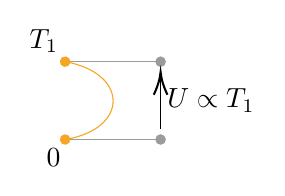
\begin{tikzpicture}[x=0.75pt,y=0.75pt,yscale=-1,xscale=1]
%uncomment if require: \path (0,110); %set diagram left start at 0, and has height of 110

%Straight Lines [id:da7792536568228223] 
\draw [color={rgb, 255:red, 155; green, 155; blue, 155 }  ,draw opacity=1 ]   (56.5,30) -- (102.5,30) ;
\draw [shift={(102.5,30)}, rotate = 0] [color={rgb, 255:red, 155; green, 155; blue, 155 }  ,draw opacity=1 ][fill={rgb, 255:red, 155; green, 155; blue, 155 }  ,fill opacity=1 ][line width=0.75]      (0, 0) circle [x radius= 2.01, y radius= 2.01]   ;
%Straight Lines [id:da7167294427341737] 
\draw [color={rgb, 255:red, 155; green, 155; blue, 155 }  ,draw opacity=1 ]   (56.5,67.5) -- (102.5,67.5) ;
\draw [shift={(102.5,67.5)}, rotate = 0] [color={rgb, 255:red, 155; green, 155; blue, 155 }  ,draw opacity=1 ][fill={rgb, 255:red, 155; green, 155; blue, 155 }  ,fill opacity=1 ][line width=0.75]      (0, 0) circle [x radius= 2.01, y radius= 2.01]   ;
%Straight Lines [id:da9591304964904978] 
\draw    (102.5,62.5) -- (102.5,37) ;
\draw [shift={(102.5,35)}, rotate = 450] [color={rgb, 255:red, 0; green, 0; blue, 0 }  ][line width=0.75]    (10.93,-3.29) .. controls (6.95,-1.4) and (3.31,-0.3) .. (0,0) .. controls (3.31,0.3) and (6.95,1.4) .. (10.93,3.29)   ;
%Curve Lines [id:da009398754899943462] 
\draw [color={rgb, 255:red, 245; green, 166; blue, 35 }  ,draw opacity=1 ]   (56.5,30) .. controls (87.33,35.5) and (87.33,62.5) .. (56.5,67.5) ;
\draw [shift={(56.5,67.5)}, rotate = 170.79] [color={rgb, 255:red, 245; green, 166; blue, 35 }  ,draw opacity=1 ][fill={rgb, 255:red, 245; green, 166; blue, 35 }  ,fill opacity=1 ][line width=0.75]      (0, 0) circle [x radius= 2.01, y radius= 2.01]   ;
\draw [shift={(56.5,30)}, rotate = 10.11] [color={rgb, 255:red, 245; green, 166; blue, 35 }  ,draw opacity=1 ][fill={rgb, 255:red, 245; green, 166; blue, 35 }  ,fill opacity=1 ][line width=0.75]      (0, 0) circle [x radius= 2.01, y radius= 2.01]   ;
% Text Node
\draw (54.5,27) node [anchor=south east] [inner sep=0.75pt]   [align=left] {$T_{1}$};
% Text Node
\draw (55.5,70.5) node [anchor=north east] [inner sep=0.75pt]   [align=left] {\SI{0}{\celsius}};
% Text Node
\draw (104.5,48.75) node [anchor=west] [inner sep=0.75pt]   [align=left] {$U \propto T_{1}$};
\end{tikzpicture}
\end{figure}
On peut déterminer $U$ à partir d'une température lorsqu'on connait précisément la mesure de $U$ à la valeur $T_2 = \SI{0}{\celsius}$. 
\end{exemple}

\subsubsection{Effet pyroélectrique}

Certains cristaux sont dits \emph{pyroélectriques} (le sulfate de triglycine par exemple) et présentent donc la propriété de présenter une polarisation électrique spontanée dépendant de la température du cristal. Ils comportent à leur surface des charges électriques $Q$ sur leurs surfaces et $-Q$ sur les surfaces opposées, proportionnelles à cette polarisation.



\begin{exemple}{Application de l'effet pyroélectrique}{}
~\\
\begin{figure}[H]

%lien d'édition des figures Tikz sur le site mathcha.io (rajouter le lien d'une modification effectuée sur la figure tikz avec le nom du modificateur car il n'y a qu'un lien par compte)

%lien mathcha Nom Prénom : https://www.mathcha.io/editor/5QmlWTYniVvh1nmzz0UV5K06oSl7KVnLfejoDdo


\tikzset{every picture/.style={line width=0.75pt}} %set default line width to 0.75pt        

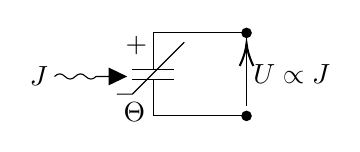
\begin{tikzpicture}[x=0.75pt,y=0.75pt,yscale=-1,xscale=1]
%uncomment if require: \path (0,110); %set diagram left start at 0, and has height of 110

%Straight Lines [id:da049441563073406525] 
\draw [color={rgb, 255:red, 0; green, 0; blue, 0 }  ,draw opacity=1 ]   (155,25) -- (200,25) ;
\draw [shift={(200,25)}, rotate = 0] [color={rgb, 255:red, 0; green, 0; blue, 0 }  ,draw opacity=1 ][fill={rgb, 255:red, 0; green, 0; blue, 0 }  ,fill opacity=1 ][line width=0.75]      (0, 0) circle [x radius= 2.01, y radius= 2.01]   ;
%Straight Lines [id:da0020140812998559188] 
\draw    (200,60) -- (200,32) ;
\draw [shift={(200,30)}, rotate = 450] [color={rgb, 255:red, 0; green, 0; blue, 0 }  ][line width=0.75]    (10.93,-3.29) .. controls (6.95,-1.4) and (3.31,-0.3) .. (0,0) .. controls (3.31,0.3) and (6.95,1.4) .. (10.93,3.29)   ;
%Straight Lines [id:da062183017724524614] 
\draw [color={rgb, 255:red, 0; green, 0; blue, 0 }  ,draw opacity=1 ]   (155,65) -- (200,65) ;
\draw [shift={(200,65)}, rotate = 0] [color={rgb, 255:red, 0; green, 0; blue, 0 }  ,draw opacity=1 ][fill={rgb, 255:red, 0; green, 0; blue, 0 }  ,fill opacity=1 ][line width=0.75]      (0, 0) circle [x radius= 2.01, y radius= 2.01]   ;
%Straight Lines [id:da18942991931898767] 
\draw    (145,42.5) -- (165,42.5) ;
%Straight Lines [id:da8438852563189819] 
\draw    (145,47.5) -- (165,47.5) ;
%Straight Lines [id:da5465187689829237] 
\draw    (155,25) -- (155,42.5) ;
%Straight Lines [id:da09145933722112254] 
\draw    (155,47.5) -- (155,65) ;

%Straight Lines [id:da8267186633709475] 
\draw    (137.5,54.5) -- (145,54.5) -- (170,29.5) ;
%Straight Lines [id:da7682659205660979] 
\draw    (107.5,46) .. controls (109.17,44.33) and (110.83,44.33) .. (112.5,46) .. controls (114.17,47.67) and (115.83,47.67) .. (117.5,46) .. controls (119.17,44.33) and (120.83,44.33) .. (122.5,46) .. controls (124.17,47.67) and (125.83,47.67) .. (127.5,46) -- (131.5,46) -- (139.5,46) ;
\draw [shift={(142.5,46)}, rotate = 180] [fill={rgb, 255:red, 0; green, 0; blue, 0 }  ][line width=0.08]  [draw opacity=0] (8.93,-4.29) -- (0,0) -- (8.93,4.29) -- cycle    ;

% Text Node
\draw (202,45) node [anchor=west] [inner sep=0.75pt]   [align=left] {$U \propto J$};
% Text Node
\draw (139.5,57.5) node [anchor=north west][inner sep=0.75pt]   [align=left] {$\Theta$};
% Text Node
\draw (140.5,25.5) node [anchor=north west][inner sep=0.75pt]   [align=left] {+};
% Text Node
\draw (105.5,46) node [anchor=east] [inner sep=0.75pt]   [align=left] {$J$};


\end{tikzpicture}

\end{figure}
On peut déterminer $U$ à partir d'un flux lumineux $J$ absorbé par un cristal pyroélectrique. Cela va élever sa température, ce qui entraîne une modification de sa polarisation qui est mesurable par la variation de tension $U$ aux bornes d'un condensateur associé.
\end{exemple}




\subsubsection{Effet piézoélectrique}

L'application d'une force ou d'une contrainte mécanique à certains matériaux dits piézoélectriques (le quartz par exemple) va entrainer une déformation provoquant l'apparition de charges électriques $Q$ sur leurs surfaces et $-Q$ sur leurs surfaces opposées.

\begin{exemple}{Application de l'effet piézoélectrique}{}
~\\
\begin{figure}[H]
\tikzset{every picture/.style={line width=0.75pt}} %set default line width to 0.75pt        

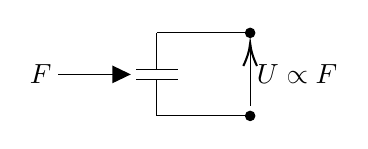
\begin{tikzpicture}[x=0.75pt,y=0.75pt,yscale=-1,xscale=1]
%uncomment if require: \path (0,110); %set diagram left start at 0, and has height of 110

%Straight Lines [id:da24742415739185752] 
\draw    (145,42.5) -- (165,42.5) ;
%Straight Lines [id:da5009949462555662] 
\draw    (145,47.5) -- (165,47.5) ;
%Straight Lines [id:da5246100942031141] 
\draw    (155,25) -- (155,42.5) ;
%Straight Lines [id:da18474784146966294] 
\draw    (155,47.5) -- (155,65) ;

%Straight Lines [id:da7890806725616728] 
\draw    (107.5,45) -- (139.5,45) ;
\draw [shift={(142.5,45)}, rotate = 180] [fill={rgb, 255:red, 0; green, 0; blue, 0 }  ][line width=0.08]  [draw opacity=0] (8.93,-4.29) -- (0,0) -- (8.93,4.29) -- cycle    ;
%Straight Lines [id:da3886370986269607] 
\draw [color={rgb, 255:red, 0; green, 0; blue, 0 }  ,draw opacity=1 ]   (155,25) -- (200,25) ;
\draw [shift={(200,25)}, rotate = 0] [color={rgb, 255:red, 0; green, 0; blue, 0 }  ,draw opacity=1 ][fill={rgb, 255:red, 0; green, 0; blue, 0 }  ,fill opacity=1 ][line width=0.75]      (0, 0) circle [x radius= 2.01, y radius= 2.01]   ;
%Straight Lines [id:da2942019649328115] 
\draw    (200,60) -- (200,32) ;
\draw [shift={(200,30)}, rotate = 450] [color={rgb, 255:red, 0; green, 0; blue, 0 }  ][line width=0.75]    (10.93,-3.29) .. controls (6.95,-1.4) and (3.31,-0.3) .. (0,0) .. controls (3.31,0.3) and (6.95,1.4) .. (10.93,3.29)   ;
%Straight Lines [id:da6965286794865602] 
\draw [color={rgb, 255:red, 0; green, 0; blue, 0 }  ,draw opacity=1 ]   (155,65) -- (200,65) ;
\draw [shift={(200,65)}, rotate = 0] [color={rgb, 255:red, 0; green, 0; blue, 0 }  ,draw opacity=1 ][fill={rgb, 255:red, 0; green, 0; blue, 0 }  ,fill opacity=1 ][line width=0.75]      (0, 0) circle [x radius= 2.01, y radius= 2.01]   ;
% Text Node
\draw (105.5,45) node [anchor=east] [inner sep=0.75pt]   [align=left] {$F$};
% Text Node
\draw (202,45) node [anchor=west] [inner sep=0.75pt]   [align=left] {$ U \propto F$};


\end{tikzpicture}
\end{figure}
On peut déterminer $U$ à partir d'une force $F$ (ou toutes grandeurs physiques dérivées) subie par l'élément piézoélectrique. Cela va provoquer une déformation de l'élément, ce qui entraine une modification de sa polarisation qui est mesurable par la variation de tension $U$ aux bornes d'un condensateur associé.
\end{exemple}


\subsubsection{Effet d'induction électromagnétique}

Lorsqu'un conducteur se déplace dans un \emph{champ magnétique} fixe $\overrightarrow{B}$, une \emph{tension} $U$ proportionnelle au \emph{flux d'induction magnétique} $\Phi$ par unité de temps $T$, et donc proportionnelle à sa vitesse de déplacement dans le champ d'induction magnétique $\overrightarrow{B}$.\\
Aussi, lorsqu'un circuit fermé est soumis à un flux d'induction magnétique $\Phi$ variable de par de son déplacement ou de celui de la source de l'induction (aimant par exemple), la tension $U$ dont il est le siège est égale au contraire de vitesse de variation du flux d'induction magnétique $\Phi$.



\begin{exemple}{Application de l'effet d'induction électromagnétique}{}
~\\
\begin{figure}[H]
\tikzset{every picture/.style={line width=0.75pt}} %set default line width to 0.75pt        

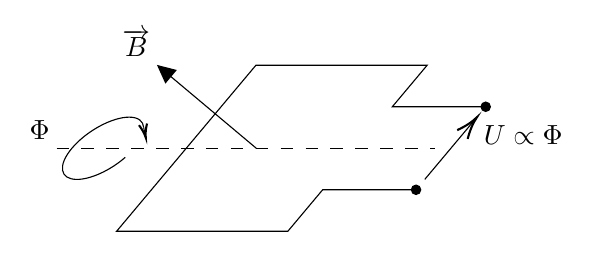
\begin{tikzpicture}[x=0.75pt,y=0.75pt,yscale=-1,xscale=1]
%uncomment if require: \path (0,156); %set diagram left start at 0, and has height of 156

%Straight Lines [id:da4159496238679624] 
\draw [color={rgb, 255:red, 0; green, 0; blue, 0 }  ,draw opacity=1 ]   (301.22,100) -- (256.22,100) -- (239.44,120) -- (156.94,120) -- (224.06,40) -- (306.56,40) -- (289.78,60) -- (334.78,60) ;
\draw [shift={(334.78,60)}, rotate = 0] [color={rgb, 255:red, 0; green, 0; blue, 0 }  ,draw opacity=1 ][fill={rgb, 255:red, 0; green, 0; blue, 0 }  ,fill opacity=1 ][line width=0.75]      (0, 0) circle [x radius= 2.01, y radius= 2.01]   ;
\draw [shift={(301.22,100)}, rotate = 180] [color={rgb, 255:red, 0; green, 0; blue, 0 }  ,draw opacity=1 ][fill={rgb, 255:red, 0; green, 0; blue, 0 }  ,fill opacity=1 ][line width=0.75]      (0, 0) circle [x radius= 2.01, y radius= 2.01]   ;
%Straight Lines [id:da9991618529346602] 
\draw    (305.41,95) -- (329.3,66.53) ;
\draw [shift={(330.59,65)}, rotate = 490] [color={rgb, 255:red, 0; green, 0; blue, 0 }  ][line width=0.75]    (10.93,-3.29) .. controls (6.95,-1.4) and (3.31,-0.3) .. (0,0) .. controls (3.31,0.3) and (6.95,1.4) .. (10.93,3.29)   ;
%Straight Lines [id:da8667170878421484] 
\draw  [dash pattern={on 4.5pt off 4.5pt}]  (128,80) -- (310.5,80) ;
%Shape: Arc [id:dp010359945518530145] 
\draw  [draw opacity=0] (161.1,84.37) .. controls (154.07,90.52) and (144.59,95) .. (137.83,95) .. controls (129.54,95) and (128.46,88.28) .. (135.41,80) .. controls (142.36,71.72) and (154.72,65) .. (163,65) .. controls (167.43,65) and (169.8,66.92) .. (169.98,69.97) -- (150.41,80) -- cycle ; \draw   (161.1,84.37) .. controls (154.07,90.52) and (144.59,95) .. (137.83,95) .. controls (129.54,95) and (128.46,88.28) .. (135.41,80) .. controls (142.36,71.72) and (154.72,65) .. (163,65) .. controls (167.43,65) and (169.8,66.92) .. (169.98,69.97) ;
%Straight Lines [id:da7991976387859124] 
\draw    (169.98,69.97) -- (170.6,72.94) ;
\draw [shift={(171.01,74.9)}, rotate = 258.2] [color={rgb, 255:red, 0; green, 0; blue, 0 }  ][line width=0.75]    (6.56,-1.97) .. controls (4.17,-0.84) and (1.99,-0.18) .. (0,0) .. controls (1.99,0.18) and (4.17,0.84) .. (6.56,1.97)   ;
%Straight Lines [id:da26501348792947876] 
\draw    (178.67,41.75) -- (224.25,80) ;
\draw [shift={(176.37,39.83)}, rotate = 40] [fill={rgb, 255:red, 0; green, 0; blue, 0 }  ][line width=0.08]  [draw opacity=0] (8.93,-4.29) -- (0,0) -- (8.93,4.29) -- cycle    ;

% Text Node
\draw (332.59,68) node [anchor=north west][inner sep=0.75pt]   [align=left] {$U \propto \Phi$};
% Text Node
\draw (174.37,36.83) node [anchor=south east] [inner sep=0.75pt]   [align=left] {$\overrightarrow{B}$};
% Text Node
\draw (126,77) node [anchor=south east] [inner sep=0.75pt]   [align=left] {$\Phi$};
\end{tikzpicture}
\end{figure}
La mesure de tension $U$ aux bornes du conducteur permet de déduire la vitesse de déplacement qui l'a induite.
\end{exemple}


\subsubsection{Effets photoélectriques}

Il existe plusieurs effets photoélectriques se distinguant par leurs manifestations mais ils ont tous comme point commun l'excitation de charges électriques dans la matière sous l'influence d'un rayonnement lumineux, dont la longueur d'onde est inférieure à une valeur seuil qui caractérise le matériau.

\begin{exemple}{Application de l'effet photoélectrique}{}
~\\
\begin{figure}[H]
\tikzset{every picture/.style={line width=0.75pt}} %set default line width to 0.75pt        

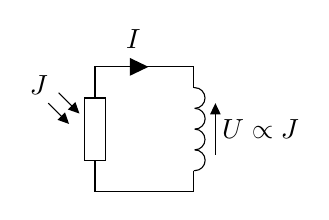
\begin{tikzpicture}[x=0.75pt,y=0.75pt,yscale=-1,xscale=1]
%uncomment if require: \path (0,153); %set diagram left start at 0, and has height of 153

%Straight Lines [id:da9553343306925111] 
\draw    (208,110.5) -- (208,115.5) ;
%Shape: Rectangle [id:dp7449879288789707] 
\draw   (213,80.5) -- (213,110.5) -- (203,110.5) -- (203,80.5) -- cycle ;
%Straight Lines [id:da5836322025533076] 
\draw    (208,75.5) -- (208,80.5) ;

%Straight Lines [id:da18940769793110568] 
\draw    (198.38,85.88) -- (190.5,78) ;
\draw [shift={(200.5,88)}, rotate = 225] [fill={rgb, 255:red, 0; green, 0; blue, 0 }  ][line width=0.08]  [draw opacity=0] (5.36,-2.57) -- (0,0) -- (5.36,2.57) -- cycle    ;
%Straight Lines [id:da5703289799533408] 
\draw    (193.38,90.88) -- (185.5,83) ;
\draw [shift={(195.5,93)}, rotate = 225] [fill={rgb, 255:red, 0; green, 0; blue, 0 }  ][line width=0.08]  [draw opacity=0] (5.36,-2.57) -- (0,0) -- (5.36,2.57) -- cycle    ;


%Straight Lines [id:da18160568852549952] 
\draw [color={rgb, 255:red, 0; green, 0; blue, 0 }  ,draw opacity=1 ]   (208,75.5) -- (208,65.5) -- (255.5,65.5) -- (255.5,75.5) ;
%Shape: Boxed Line [id:dp8550958962997346] 
\draw [color={rgb, 255:red, 0; green, 0; blue, 0 }  ,draw opacity=1 ]   (255.5,115.5) -- (255.5,125.5) -- (208,125.5) -- (208,115.5) ;
%Shape: Arc [id:dp9236278998461147] 
\draw  [draw opacity=0] (255.71,75.51) .. controls (255.81,75.5) and (255.9,75.5) .. (256,75.5) .. controls (258.76,75.5) and (261,77.74) .. (261,80.5) .. controls (261,83.25) and (258.78,85.48) .. (256.04,85.5) -- (256,80.5) -- cycle ; \draw   (255.71,75.51) .. controls (255.81,75.5) and (255.9,75.5) .. (256,75.5) .. controls (258.76,75.5) and (261,77.74) .. (261,80.5) .. controls (261,83.25) and (258.78,85.48) .. (256.04,85.5) ;
%Shape: Arc [id:dp01043642876607509] 
\draw  [draw opacity=0] (256.04,85.5) .. controls (256.05,85.5) and (256.05,85.5) .. (256.06,85.5) .. controls (258.82,85.5) and (261.06,87.74) .. (261.06,90.5) .. controls (261.06,93.25) and (258.84,95.48) .. (256.1,95.5) -- (256.06,90.5) -- cycle ; \draw   (256.04,85.5) .. controls (256.05,85.5) and (256.05,85.5) .. (256.06,85.5) .. controls (258.82,85.5) and (261.06,87.74) .. (261.06,90.5) .. controls (261.06,93.25) and (258.84,95.48) .. (256.1,95.5) ;
%Shape: Arc [id:dp6271751911575147] 
\draw  [draw opacity=0] (255.98,95.5) .. controls (255.99,95.5) and (255.99,95.5) .. (256,95.5) .. controls (258.76,95.5) and (261,97.74) .. (261,100.5) .. controls (261,103.25) and (258.78,105.48) .. (256.04,105.5) -- (256,100.5) -- cycle ; \draw   (255.98,95.5) .. controls (255.99,95.5) and (255.99,95.5) .. (256,95.5) .. controls (258.76,95.5) and (261,97.74) .. (261,100.5) .. controls (261,103.25) and (258.78,105.48) .. (256.04,105.5) ;
%Shape: Arc [id:dp7604597461390405] 
\draw  [draw opacity=0] (256.04,105.5) .. controls (256.05,105.5) and (256.05,105.5) .. (256.06,105.5) .. controls (258.82,105.5) and (261.06,107.74) .. (261.06,110.5) .. controls (261.06,113.26) and (258.82,115.5) .. (256.06,115.5) .. controls (255.9,115.5) and (255.74,115.49) .. (255.59,115.48) -- (256.06,110.5) -- cycle ; \draw   (256.04,105.5) .. controls (256.05,105.5) and (256.05,105.5) .. (256.06,105.5) .. controls (258.82,105.5) and (261.06,107.74) .. (261.06,110.5) .. controls (261.06,113.26) and (258.82,115.5) .. (256.06,115.5) .. controls (255.9,115.5) and (255.74,115.49) .. (255.59,115.48) ;

%Straight Lines [id:da7979642956460348] 
\draw    (266,86) -- (266,108) ;
\draw [shift={(266,83)}, rotate = 90] [fill={rgb, 255:red, 0; green, 0; blue, 0 }  ][line width=0.08]  [draw opacity=0] (5.36,-2.57) -- (0,0) -- (5.36,2.57) -- cycle    ;
%Straight Lines [id:da6970578975487184] 
\draw    (232.75,65.5) -- (255.5,65.5) ;
\draw [shift={(233.75,65.5)}, rotate = 180] [fill={rgb, 255:red, 0; green, 0; blue, 0 }  ][line width=0.08]  [draw opacity=0] (8.93,-4.29) -- (0,0) -- (8.93,4.29) -- cycle    ;

% Text Node
\draw (186.5,80) node [anchor=south east] [inner sep=0.75pt]   [align=left] {$J$};
% Text Node
\draw (268,95.5) node [anchor=west] [inner sep=0.75pt]   [align=left] {$U \propto J$};
% Text Node
\draw (226.5,58) node [anchor=south] [inner sep=0.75pt]   [align=left] {$I$};


\end{tikzpicture}
\end{figure}
Les effets photoélectriques permettent d'obtenir une tension $U$ ou un courant $I$ en fonction du rayonnement lumineux $J$ du matériau. D'une part, ils constituent la base des méthodes de mesure des grandeurs photométriques, d'autre part, ils permettent la traduction en signal électriques des informations véhiculées par un rayonnement lumineux.
\end{exemple}



\subsubsection{Effets photoémissif}

Les électrons libérés sont émis hors d'une zone éclairée et, lors de l'application d'un champ électrique, forment un courant électrique.

\subsubsection{Effets photovoltaïque}

Des électrons et des trous pouvant recevoir des électrons sont libérés au voisinage de la jonction Positive Négative (PN) d'un semi-conducteur éclairée. Leur déplacement dans le champ électrique de la jonction PN module la tension aux bornes de cette jonction.

\subsubsection{Effet photoélectromagnétique}

L'application d'un champ magnétique perpendiculaire à un rayonnement lumineux va provoquer dans le matériaux éclairé l'apparition d'une tension électrique dans la direction \emph{normale} au champ magnétique et au rayonnement.

\subsubsection{Effet Hall}

Un matériau, de préférence semi-conducteur et sous forme de plaquette, fait apparaitre une tension $v_{H}$ lorsqu'il est parcouru par un courant $I$ et soumis à un champ magnétique $\overrightarrow{B}$ d'un angle $\theta$ avec le courant $I$.

\begin{formule}{Effet Hall}{effet_hall}
\begin{align*}
v_H &= K_H \times I \times B \times \sin\theta
\end{align*}

\begin{textvariables}
\K_H							& coefficient	& 				& 		/											& 	Facteur dépendant du matériau et de la dimension de la plaquette \\
I									& intensité		& 	ampère			& 		\ampere					& Source de courant fournissant l'énergie liée au signal de sortie  \\
\overrightarrow{B}									& champ magnétique		& Tesla		& \tesla						& Champ magnétique soumis au matériau \\
\sin\theta					& angle							& radian		& \radian				& Angle formé par l'intensité $I$ et le champ magnétique $\overrightarrow{B}$ \\
\end{textvariables}
\end{formule}


\begin{exemple}{Application de l'effet Hall}{}
~\\
\begin{figure}[H]

\tikzset{every picture/.style={line width=0.75pt}} %set default line width to 0.75pt        

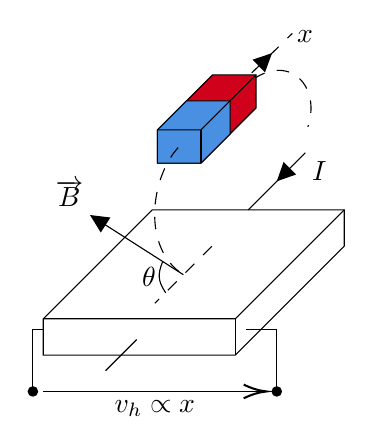
\begin{tikzpicture}[x=0.75pt,y=0.75pt,yscale=-1,xscale=1]
%uncomment if require: \path (0,255); %set diagram left start at 0, and has height of 255

%Curve Lines [id:da026480600050421743] 
\draw  [dash pattern={on 4.5pt off 4.5pt}]  (390,37.5) .. controls (411.6,12.4) and (432.3,30.3) .. (425,52.5) ;
%Shape: Cube [id:dp07360762187167524] 
\draw  [fill={rgb, 255:red, 208; green, 2; blue, 27 }  ,fill opacity=1 ] (352.5,54.06) -- (379.06,27.5) -- (400,27.5) -- (400,43.44) -- (373.44,70) -- (352.5,70) -- cycle ; \draw   (400,27.5) -- (373.44,54.06) -- (352.5,54.06) ; \draw   (373.44,54.06) -- (373.44,70) ;
%Shape: Cube [id:dp18529556990685714] 
\draw  [fill={rgb, 255:red, 74; green, 144; blue, 226 }  ,fill opacity=1 ] (352.5,54) -- (366.5,40) -- (387.5,40) -- (387.5,56) -- (373.5,70) -- (352.5,70) -- cycle ; \draw   (387.5,40) -- (373.5,54) -- (352.5,54) ; \draw   (373.5,54) -- (373.5,70) ;

%Shape: Cube [id:dp5559755925236529] 
\draw   (297.5,145) -- (350,92.5) -- (442.5,92.5) -- (442.5,110) -- (390,162.5) -- (297.5,162.5) -- cycle ; \draw   (442.5,92.5) -- (390,145) -- (297.5,145) ; \draw   (390,145) -- (390,162.5) ;
%Straight Lines [id:da7084755043157218] 
\draw    (327.5,170) -- (342.5,155) ;
%Straight Lines [id:da9878757017878151] 
\draw    (396.25,92.5) -- (423.75,65) ;
\draw [shift={(410,78.75)}, rotate = 315] [fill={rgb, 255:red, 0; green, 0; blue, 0 }  ][line width=0.08]  [draw opacity=0] (8.93,-4.29) -- (0,0) -- (8.93,4.29) -- cycle    ;
%Straight Lines [id:da6115380075011939] 
\draw    (297.5,145) -- (390,145) ;
%Straight Lines [id:da8865101665838837] 
\draw  [dash pattern={on 4.5pt off 4.5pt}]  (378.75,110) -- (351.25,137.5) ;
%Straight Lines [id:da4151864093884584] 
\draw    (322.53,96.62) -- (365,123.75) ;
\draw [shift={(320,95)}, rotate = 32.57] [fill={rgb, 255:red, 0; green, 0; blue, 0 }  ][line width=0.08]  [draw opacity=0] (8.93,-4.29) -- (0,0) -- (8.93,4.29) -- cycle    ;
%Straight Lines [id:da13161923838594092] 
\draw  [dash pattern={on 4.5pt off 4.5pt}]  (397.97,26.5) -- (417.5,7.5) ;
\draw [shift={(407.73,17)}, rotate = 495.79] [fill={rgb, 255:red, 0; green, 0; blue, 0 }  ][line width=0.08]  [draw opacity=0] (8.93,-4.29) -- (0,0) -- (8.93,4.29) -- cycle    ;
%Curve Lines [id:da8220459438720412] 
\draw  [dash pattern={on 4.5pt off 4.5pt}]  (362.5,62.5) .. controls (349.4,76.7) and (344.6,110.7) .. (365,123.75) ;
%Curve Lines [id:da48302895341966623] 
\draw    (355,117.5) .. controls (352.6,123.5) and (352.6,126.7) .. (356.5,132.5) ;
%Straight Lines [id:da0016723825185572805] 
\draw    (410,180) -- (410,150) -- (395,150) ;
\draw [shift={(410,180)}, rotate = 270] [color={rgb, 255:red, 0; green, 0; blue, 0 }  ][fill={rgb, 255:red, 0; green, 0; blue, 0 }  ][line width=0.75]      (0, 0) circle [x radius= 2.01, y radius= 2.01]   ;
%Straight Lines [id:da6665646722680143] 
\draw    (292.5,180) -- (292.5,150) -- (297.5,150) ;
\draw [shift={(292.5,180)}, rotate = 270] [color={rgb, 255:red, 0; green, 0; blue, 0 }  ][fill={rgb, 255:red, 0; green, 0; blue, 0 }  ][line width=0.75]      (0, 0) circle [x radius= 2.01, y radius= 2.01]   ;
%Straight Lines [id:da45157029340764043] 
\draw    (297.5,180) -- (403,180) ;
\draw [shift={(405,180)}, rotate = 180] [color={rgb, 255:red, 0; green, 0; blue, 0 }  ][line width=0.75]    (10.93,-3.29) .. controls (6.95,-1.4) and (3.31,-0.3) .. (0,0) .. controls (3.31,0.3) and (6.95,1.4) .. (10.93,3.29)   ;

% Text Node
\draw (425.75,68) node [anchor=north west][inner sep=0.75pt]   [align=left] {$I$};
% Text Node
\draw (318,92) node [anchor=south east] [inner sep=0.75pt]   [align=left] {$\overrightarrow{B}$};
% Text Node
\draw (353,125) node [anchor=east] [inner sep=0.75pt]   [align=left] {$\theta$};
% Text Node
\draw (418.5,5) node [anchor=north west][inner sep=0.75pt]   [align=left] {$x$};
% Text Node
\draw (351.25,183) node [anchor=north] [inner sep=0.75pt]   [align=left] {$v_{h} \propto x$};

\end{tikzpicture}
\end{figure}
Pour connaître la position de l'objet, on lui accouple un aimant qui va lui déterminer les valeurs de $\overrightarrow{B}$ et $\theta$ au niveau de la plaquette. La tension $v_{h}$ aux bornes de la plaquette est donc fonction de cet aimant et permet une conversion électrique d'une position $x$.
\end{exemple}



Il convient de classer les capteurs basés sur l'effet Hall parmi les capteurs actifs puisque l'information sortie est liée à une tension $v_H$, quand bien même il ne s'agit pas de \emph{convertisseurs d'énergie} car c'est une source de courant $I$  et non le mesurande qui va délivrer l'énergie liée au signal de sortie.

\subsection{Capteurs passifs}

Les capteurs passifs sont donc des \emph{récepteurs} qui vont voir leurs grandeurs physiques être modulées par le mesurande sans pour autant convertir une énergie. On distingue dans les récepteurs plusieurs grandeurs physiques liées à :
\begin{itemize}
\item leur géométrie et leurs dimensions\,;
\item leurs propriétés électriques :
\begin{itemize}
\item résistivité $\rho$\,;
\item perméabilité magnétique $\mu$\,;
\item constante diélectrique $\varepsilon$.
\end{itemize}
\end{itemize}

Un mesurande module donc sur la variation du signal de sortie électrique du capteur passif :
\begin{itemize}
\item soit par les caractéristiques géométriques ou des dimensions\,;
\item soit par les propriétés électriques des matériaux\,;
\item soit plus rarement par les deux à la fois.
\end{itemize}

\subsubsection{Paramètres géométrique et dimensionnel du capteur passif}

Pour que les paramètres géométriques ou dimensionnels du capteur passif puissent varier, il faut que le capteur comporte des éléments mobiles ou déformables.\\

\paragraph{Position}

Le principe d'une majorité de capteurs de déplacement et de position se base sur un élément mobile du capteur qui présente des positions spécifiques pour des valeurs de sorties précises. La mesure de cette valeur de sortie permet de connaître la position de l'élément mobile (potentiomètre, condensateur à armature mobile, inductance à noyau mobile\ldots).

\paragraph{Déformation}

La déformation est la résultante de forces -- ou de grandeurs dérivées --  qui est appliquée directement ou indirectement sur un capteur (armature d'un condensateur soumis à une pression différentielle, jauge d'extensométrie liée de manière rigide à une structure contrainte\ldots).\\
Cela entraine une modification du signal du sortie $s$, qui sera corrélée à la valeur de la force appliquée sur le capteur.

\paragraph{Propriétés électriques des matériaux}

Les propriétés électriques des matériaux varient selon leur nature et sont également sensibles à diverses grandeurs physiques (température, pression, humidité, éclairement\ldots).\\
Dans le cas ou seule l'une de ces grandeurs est susceptible de modifier les propriétés électriques d'un matériau mais que les autres n'influencent pas ces mêmes propriétés, il s'établit alors une corrélation entre ces cette grandeur physique et le signal de sortie $s$.

\begin{table}[H]
\caption{Capteurs passifs principaux selon les effets physiques}

\begin{tabularx}{\linewidth}{XX>{\compress}X}
\toprule
\thead{Mesurande}						&	\thead{Caractéristique électrique sensible}					&	\thead{Matériau utilisé} \\
\midrule
Température									& Résistivité						& 
\begin{tabitemize}
\item métaux (platine, cuivre, nickel)\,;
\item semi-conducteurs.
\end{tabitemize}
 \\
 Très basse température				& Constante diélectrique				& Verre \\
\addlinespace
Flux de rayonnement optique			& Résistivité									& Semi-conducteurs \\
\addlinespace
Déformation									& 	Résistivité		 											& \begin{tabitemize}
\item alliages de nickel\,;
\item silicium dopé.
\end{tabitemize}
 \\
													& 	Perméabilité magnétique						& 	Alliages ferromagnétiques		 \\
\addlinespace
Position (aimant)											& 	Résistivité		& 	Matériaux magnéto-résistant (bismuth, antimoniure d'indium)		 \\
\addlinespace
Humidité									&  Résistivité													& 	Chlorure de lithium		 \\
									&  Constante diélectrique								& 	Alumine, polymères		 \\
\addlinespace
Niveau							& 	Constante diélectrique								& Liquides isolants \\
\bottomrule
\end{tabularx}
\end{table}

Dans le tableau ci-dessus, on remarque l'importe de la propriété de la \emph{résistivité} $\rhoup$.\\
Le signal de sortie $s$ des \emph{capteurs passifs} n'est mesurable qu'en intégrant le capteur dans un circuit électrique alimenté, désigné comme étant son \emph{conditionneur}. Ils en existe plusieurs sortes dont les principaux sont les suivants :
\begin{description}
\item [montage potentiométrique :] association \emph{en série} d'un capteur et d'une impédance pouvant être ou non du même type\,;
\item [pont d'impédances :] équilibre électrique du pont permettant la détermination de l'impédance de sortie du capteur ou déséquilibre du pont permettant la mesure de la variation de cette impédance\,;
\item [circuit oscillant :] circuit contenant l'impédance du capteur et faisant partie d'un circuit oscillateur dont il détermine la fréquence\,;
\item [amplificateur opérationnel :] circuit dont l'impédance du capteur constitue l'un des éléments déterminant le gain de l'amplificateur.
\end{description}

Choisir un \emph{conditionneur} est une étape primordiale dans la réalisation de mesures. L'association d'un capteur et de son conditionneur -- dont sa constitution -- déterminera le signal électrique et en découleront un bon nombre de performances de mesures :
\begin{itemize}
\item sensibilité\,;
\item linéarité\,;
\item insensibilité à certaines grandeurs d'influences.
\end{itemize}

\section{Corps d'épreuves et capteurs composites}

Pour certaines raisons (coût, facilité d'exploitation\ldots), on peut utiliser des capteur sensible à l'un des effets du \emph{mesurande} plutôt qu'au mesurande lui-même.

\begin{definition}{Corps d'épreuve}{}
Dispositif de mesure qui, une fois soumis à un mesurande désigné \emph{mesurande primaire} dont il faut connaitre la grandeur, assure la traduction en une autre grandeur physique non-électrique désignée \emph{mesurande secondaire}.
\end{definition}
\begin{definition}{Capteur composite}{}
Ensemble formé par le corps d'épreuve et un capteur passif ou actif nécessaire à la traduction du mesurande secondaire donnée par le corps d'épreuve.
\end{definition}

%--------------------------------------
%CANEVAS
%--------------------------------------

%utiliser les environnement \begin{comment} \end{comment} pour mettre en commentaire le préambule une fois la programmation appelée dans le document maître (!ne pas oublier de mettre en commentaire \end{document}!)

\begin{comment}

\documentclass[a4paper, 11pt, twoside, fleqn]{memoir}

\usepackage{AOCDTF}

\marqueurchapitre
\decoupagechapitre{1} %juste pour éviter les erreurs lors de la compilation des sous-programmations (passera en commentaire)

%lien d'édition des figures Tikz sur le site mathcha.io (rajouter le lien d'une modification effectuée sur la figure tikz avec le nom du modificateur car il n'y a qu'un lien par compte) 

%lien mathcha Nom Prénom : https://www.mathcha.io/editor/88XmJTWQUxztLv21v6S12z22Lf78mx9yIOvQ9M5

%--------------------------------------
%corps du document
%--------------------------------------

\begin{document} %corps du document
	\openleft %début de chapitre à gauche

\end{comment}

\begin{figure}[h]
\caption{Structure d'un corps d'épreuve}

\tikzset{every picture/.style={line width=0.75pt}} %set default line width to 0.75pt        

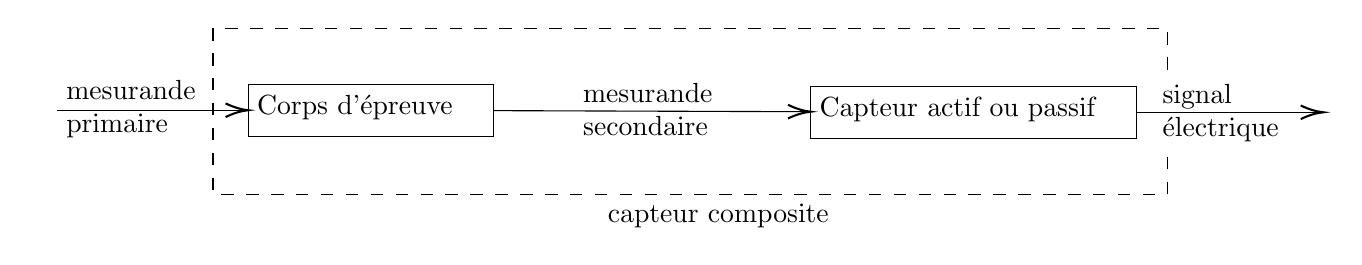
\begin{tikzpicture}[x=0.75pt,y=0.75pt,yscale=-1,xscale=1]
%uncomment if require: \path (0,300); %set diagram left start at 0, and has height of 300

%Straight Lines [id:da6331649314862131] 
\draw  [dash pattern={on 4.5pt off 4.5pt}]  (550,120) -- (550,100) -- (90,100) -- (90,180) -- (550,180) -- (550,160) ;

% Text Node
\draw    (107,127) -- (225,127) -- (225,152) -- (107,152) -- cycle  ;
\draw (110,131) node [anchor=north west][inner sep=0.75pt]   [align=left] {Corps d'épreuve};
% Text Node
\draw    (378,128) -- (535,128) -- (535,153) -- (378,153) -- cycle  ;
\draw (381,132) node [anchor=north west][inner sep=0.75pt]   [align=left] {Capteur actif ou passif};
% Text Node
\draw (1,131) node [anchor=north west][inner sep=0.75pt]   [align=left] {};
% Text Node
\draw (50.5,139) node   [align=left] {mesurande\\primaire};
% Text Node
\draw (299.5,139) node   [align=left] {mesurande\\secondaire};
% Text Node
\draw (628,132) node [anchor=north west][inner sep=0.75pt]   [align=left] {};
% Text Node
\draw (575.5,141) node   [align=left] {signal\\électrique};
% Text Node
\draw (333.5,190.5) node   [align=left] {capteur composite};
% Connection
\draw    (225,139.7) -- (376,140.22) ;
\draw [shift={(378,140.23)}, rotate = 180.2] [color={rgb, 255:red, 0; green, 0; blue, 0 }  ][line width=0.75]    (10.93,-3.29) .. controls (6.95,-1.4) and (3.31,-0.3) .. (0,0) .. controls (3.31,0.3) and (6.95,1.4) .. (10.93,3.29)   ;
% Connection
\draw    (15,139.5) -- (105,139.5) ;
\draw [shift={(107,139.5)}, rotate = 180] [color={rgb, 255:red, 0; green, 0; blue, 0 }  ][line width=0.75]    (10.93,-3.29) .. controls (6.95,-1.4) and (3.31,-0.3) .. (0,0) .. controls (3.31,0.3) and (6.95,1.4) .. (10.93,3.29)   ;
% Connection
\draw    (535,140.5) -- (623,140.5) ;
\draw [shift={(625,140.5)}, rotate = 180] [color={rgb, 255:red, 0; green, 0; blue, 0 }  ][line width=0.75]    (10.93,-3.29) .. controls (6.95,-1.4) and (3.31,-0.3) .. (0,0) .. controls (3.31,0.3) and (6.95,1.4) .. (10.93,3.29)   ;

\end{tikzpicture}
\end{figure}

%\end{document}



\begin{exemple}{Application d'un capteur composite}{}
Une force de traction $F$ est appliquée sur un objet d'une section $S$ et d'une longueur $L$, qui va subir un allongement de sa longueur $\frac{\Delta L}{L}$, entrainant de ce fait une variation de la résistance d'une jauge \Circled{1} d'un facteur $K$ placée sur l'objet $\frac{\Delta R}{R}$.
\begin{formule*}{Module de Young}{}
\begin{align*}
		E 	&= \frac{\varepsilon}{\sigma}
\end{align*}
\begin{textvariables}
E 					& Pression		&	Pascal			& \pascal 				& Module de Young (de traction) d'un matérieau \emph{élastique} et \emph{isotope} \\ 
\varepsilon	& Mètre			& 	Mètre			& \meter				& Allongement relatif (déformation) $\frac{\Delta L}{L}$ \\
 \sigma			& Pression		&	Pascal			& \pascal				& contrainte sur le matériau \\
\end{textvariables}
\end{formule*}

\begin{center}
%https://www.mathcha.io/editor/Gq5WKTE5SOVh1Y2BNvf3MWGXJHB9DB8dFlvmpqK
% Pattern Info
 
\tikzset{
pattern size/.store in=\mcSize, 
pattern size = 5pt,
pattern thickness/.store in=\mcThickness, 
pattern thickness = 0.3pt,
pattern radius/.store in=\mcRadius, 
pattern radius = 1pt}
\makeatletter
\pgfutil@ifundefined{pgf@pattern@name@_23ewa924x}{
\pgfdeclarepatternformonly[\mcThickness,\mcSize]{_23ewa924x}
{\pgfqpoint{0pt}{0pt}}
{\pgfpoint{\mcSize+\mcThickness}{\mcSize+\mcThickness}}
{\pgfpoint{\mcSize}{\mcSize}}
{
\pgfsetcolor{\tikz@pattern@color}
\pgfsetlinewidth{\mcThickness}
\pgfpathmoveto{\pgfqpoint{0pt}{0pt}}
\pgfpathlineto{\pgfpoint{\mcSize+\mcThickness}{\mcSize+\mcThickness}}
\pgfusepath{stroke}
}}
\makeatother
\tikzset{every picture/.style={line width=0.5pt}} %set default line width to 0.75pt        

\begin{tikzpicture}[x=0.75pt,y=0.75pt,yscale=-0.6,xscale=0.6]
%uncomment if require: \path (0,300); %set diagram left start at 0, and has height of 300

%Shape: Can [id:dp12472449649523132] 
\draw   (134.92,100) -- (345.08,100) .. controls (350.56,100) and (355,113.43) .. (355,130) .. controls (355,146.57) and (350.56,160) .. (345.08,160) -- (134.92,160) .. controls (129.44,160) and (125,146.57) .. (125,130) .. controls (125,113.43) and (129.44,100) .. (134.92,100) .. controls (140.39,100) and (144.83,113.43) .. (144.83,130) .. controls (144.83,146.57) and (140.39,160) .. (134.92,160) ;
%Straight Lines [id:da5161240947796851] 
\draw    (135,130) -- (98,130) ;
\draw [shift={(95,130)}, rotate = 360] [fill={rgb, 255:red, 0; green, 0; blue, 0 }  ][line width=0.08]  [draw opacity=0] (8.93,-4.29) -- (0,0) -- (8.93,4.29) -- cycle    ;
%Straight Lines [id:da28806277731694174] 
\draw    (382,130) -- (355,130) ;
\draw [shift={(385,130)}, rotate = 180] [fill={rgb, 255:red, 0; green, 0; blue, 0 }  ][line width=0.08]  [draw opacity=0] (8.93,-4.29) -- (0,0) -- (8.93,4.29) -- cycle    ;
%Straight Lines [id:da3487762389054402] 
\draw  [dash pattern={on 4.5pt off 4.5pt}]  (134.92,165) -- (135,185) ;
%Straight Lines [id:da07803041607897865] 
\draw  [dash pattern={on 4.5pt off 4.5pt}]  (344.92,165) -- (345,185) ;
%Straight Lines [id:da4638976844778334] 
\draw    (137,185) -- (343,185) ;
\draw [shift={(345,185)}, rotate = 180] [color={rgb, 255:red, 0; green, 0; blue, 0 }  ][line width=0.75]    (10.93,-3.29) .. controls (6.95,-1.4) and (3.31,-0.3) .. (0,0) .. controls (3.31,0.3) and (6.95,1.4) .. (10.93,3.29)   ;
\draw [shift={(135,185)}, rotate = 0] [color={rgb, 255:red, 0; green, 0; blue, 0 }  ][line width=0.75]    (10.93,-3.29) .. controls (6.95,-1.4) and (3.31,-0.3) .. (0,0) .. controls (3.31,0.3) and (6.95,1.4) .. (10.93,3.29)   ;
%Shape: Ellipse [id:dp48131477454456484] 
\draw  [pattern=_23ewa924x,pattern size=6pt,pattern thickness=0.75pt,pattern radius=0pt, pattern color={rgb, 255:red, 0; green, 0; blue, 0}] (125,130) .. controls (125,113.43) and (129.44,100) .. (134.92,100) .. controls (140.39,100) and (144.83,113.43) .. (144.83,130) .. controls (144.83,146.57) and (140.39,160) .. (134.92,160) .. controls (129.44,160) and (125,146.57) .. (125,130) -- cycle ;
%Shape: Rectangle [id:dp9836272663606409] 
\draw  [fill={rgb, 255:red, 0; green, 0; blue, 0 }  ,fill opacity=1 ] (240,152.5) -- (270,152.5) -- (270,160) -- (240,160) -- cycle ;

% Text Node
\draw (93,130) node [anchor=east] [inner sep=0.75pt]   [align=left] {$F$};
% Text Node
\draw (387,130) node [anchor=west] [inner sep=0.75pt]   [align=left] {$F$};
% Text Node
\draw (240,188) node [anchor=north] [inner sep=0.75pt]   [align=left] {$L$};
% Text Node
\draw (91,65) node [anchor=north west][inner sep=0.75pt]   [align=left] {$S$};
% Text Node
\draw (134.92,130) node   [align=left] {};
% Text Node
\draw (272,149.5) node [anchor=south west] [inner sep=0.75pt]   [align=left] {\Circled{1}};
% Connection
\draw    (105,86.39) -- (125.29,115.96) ;
\draw [shift={(126.42,117.61)}, rotate = 235.55] [color={rgb, 255:red, 0; green, 0; blue, 0 }  ][line width=0.75]    (10.93,-3.29) .. controls (6.95,-1.4) and (3.31,-0.3) .. (0,0) .. controls (3.31,0.3) and (6.95,1.4) .. (10.93,3.29)   ;

\end{tikzpicture}
\end{center}


Dans l'exemple la relation entre le mesurande primaire, la traction $F$ et le mesurande secondaire, la déformation $\frac{\Delta L}{L}$, est :
\begin{align*}
\frac{\Delta L}{L} &= \frac{1}{E} \times \frac{F}{S} 
\end{align*}
D'autre part, la relation entre la grandeur de sortie, la variation de la résistance de la jauge $\frac{\Delta R}{R}$ et le mesurande secondaire, la déformation $\frac{\Delta L}{L}$ est :
\begin{align*}
\frac{\Delta R}{R} &= K \times \frac{\Delta L}{L}
\end{align*}
La relation de la variation de la résistance de la jauge $R$ et la traction :
\begin{align*}
\frac{\Delta R}{R} &= \frac{K}{E} \times \frac{F}{S} 
\end{align*}
\end{exemple}

Les corps d'épreuves sont très utilisés pour mesurer des grandeurs physiques en mécanique.\\
La relation entre le mesurande primaire et le mesurande secondaire est très souvent linéaire, en particulier dans le cas de déformations et déplacement résultants de contraintes mécaniques, dans les conditions limites de l'élasticité du corps d'épreuve. Les performances de l'association corps d'épreuve -- capteur doivent être déterminées par un étalonnage tenant compte des éventuelles conséquences de leur liaison par rapport à leurs caractéristiques individuelles.\\
Si de l'électronique est intégrée au capteur, il s'agira d'un \emph{capteur intégré}.

\section{Grandeurs d'influence}

Un capteur se situe dans un environnement qui le soumet à un mesurande mais également à d'autres grandeurs physiques susceptibles de biaiser la valeur de la grandeur de sortie, sans distinction d'origine du biais.

\begin{definition}{Grandeur d'influence}{}
Grandeur physique \og parasite \fg{} à laquelle la réponse d'un capteur peut être sensible.
\end{definition}

On distingue par exemple :
\begin{itemize}
\item température pouvant faire varier la réponse d'un capteur optique\,;
\item champ magnétique pouvant faire varier la réponse d'un capteur thermométrique.
\end{itemize}

Les principales grandeurs d'influences sont :
\begin{description}
\item [température :] modification des caractéristiques électriques, mécaniques et dimensionnelles des composants du capteur\,;
\item [pression, accélération, vibration :] perturbations pouvant créer des déformations et des contraintes dans certains composants du capteur, altérant ainsi sa réponse\,;
\item [humidité :] dégradation de l'isolation (capteur/environnement et composant du capteur) et perturbation de certaines propriétés électriques (constante diélectrique, résistivité\ldots)\,;
\item [champs magnétiques variables et statiques :] apparition potentielle de tension induite pouvant se superposer au signal utile en régime statique et modification des propriété électrique en régime variable\,;
\item [tension d'alimentation (amplitude et fréquence) :] grandeur de sortie du capteur dépendante de ces grandeurs de par le principe même du capteur.
\end{description}

Si l'on se réfère à la relation mesurande -- grandeur de sortie (\superref{form:grandeur_sortie}) et qu'on comptabilise l'influence de $g_1$, $g_2$\ldots, cela donne :
\begin{formule}{Grandeurs d'influence}{grandeurs_influences}
\begin{align*}
   		s &= F(m, g_1, g_2\ldots) \\
\end{align*}

\begin{textvariables}
s						& grandeur électrique	& 			& 		/					& 	Grandeur (réponse) de sortie de nature électrique (charge, tension, courant ou impédance) fonction du mesurande \\
m						& grandeur physique		& 			& 		/					& Grandeur physique d'entrée d'excitation autre qu'électrique  \\
g_1					& grandeur physique		& 			& 		/					& Grandeur physique d'influence 1  \\
g_2					& grandeur physique		& 			& 		/					& Grandeur physique d'influence 2  \\
\end{textvariables}
\end{formule}

Pour déduire la valeur de $s$ en fonction de $m$ seul, il convient de :
\begin{itemize}
\item soit de réduire l'importance des grandeurs d'influence au niveau du capteur en le protégeant par un isolement adéquat (supports antivibratoires, blindages magnétiques\ldots)\,;
\item soit de stabiliser ces grandeurs d'influences à des seuils précisément déterminés et d'étalonner le capteur dans ces conditions de fonctionnement (enceinte climatique, sources d'alimentation régulées\ldots)\,;
\item soit d'utiliser un montage pouvant compenser l'influence des perturbations. 
\end{itemize}

\section{Chaine de mesure}

\begin{definition}{Chaine de mesure}{}
Ensemble des dispositifs, y compris le capteur, dont le but est de délivrer la détermination précise de la valeur d'un mesurande dans les meilleures conditions.  
\end{definition}

En entrée de chaine, le capteur est soumis à l'action du mesurande $m$ et injectera son signal de sortie $s$ dans la chaine. En fin de chaine, le signal de sortie $s$ est converti pour rendre la lecture de la valeur du mesurande $m$ possible.
C'est l'étalonnage de la chaine de mesure dans son ensemble qui déterminera au mieux la valeur de sortie $s$ par rapport au mesurande $m$ correspondant. \\
La chaine de mesure comprend le capteur (avec son conditionneur s'il est passif) associé à un appareil de lecture dans sa forme la plus simple (thermocouple et voltmètre par exemple).\\
Toutefois, les exigences requises par les conditions d'exploitation et la recherche de performance amènent à l'introduction de nouveaux blocs fonctionnels dans la chaine de mesure. Ceux-ci servent à optimiser l'acquisition et le traitement du signal de sortie $s$, en voici les principaux :
\begin{itemize}
\item circuit de linéarisation du signal pour obtenir des données proportionnelles à celles du mesurande $m$\,;
\item amplificateur d'instrumentation ou d'isolement pour la réduction des tensions parasites de mode commun ;
\item multiplexeur, amplificateur d'instrumentation programmable, échantillonneur bloqueur, convertisseur analogique - numérique pour le traitement de l'information par calculateur (\superref{fig:exemple_chaine_mesure})\,;
\item convertisseur tension -- courant ou tension -- fréquence pour la transmission du signal à distance par câble\,;
\item modulateur de fréquence dans cas de télémesure par voie hertzienne.
\end{itemize}

\begin{figure}{\label{fig:exemple_chaine_mesure}}
\caption{Exemple d'une chaine de mesure}


\tikzset{every picture/.style={line width=0.5pt}} %set default line width to 0.75pt        

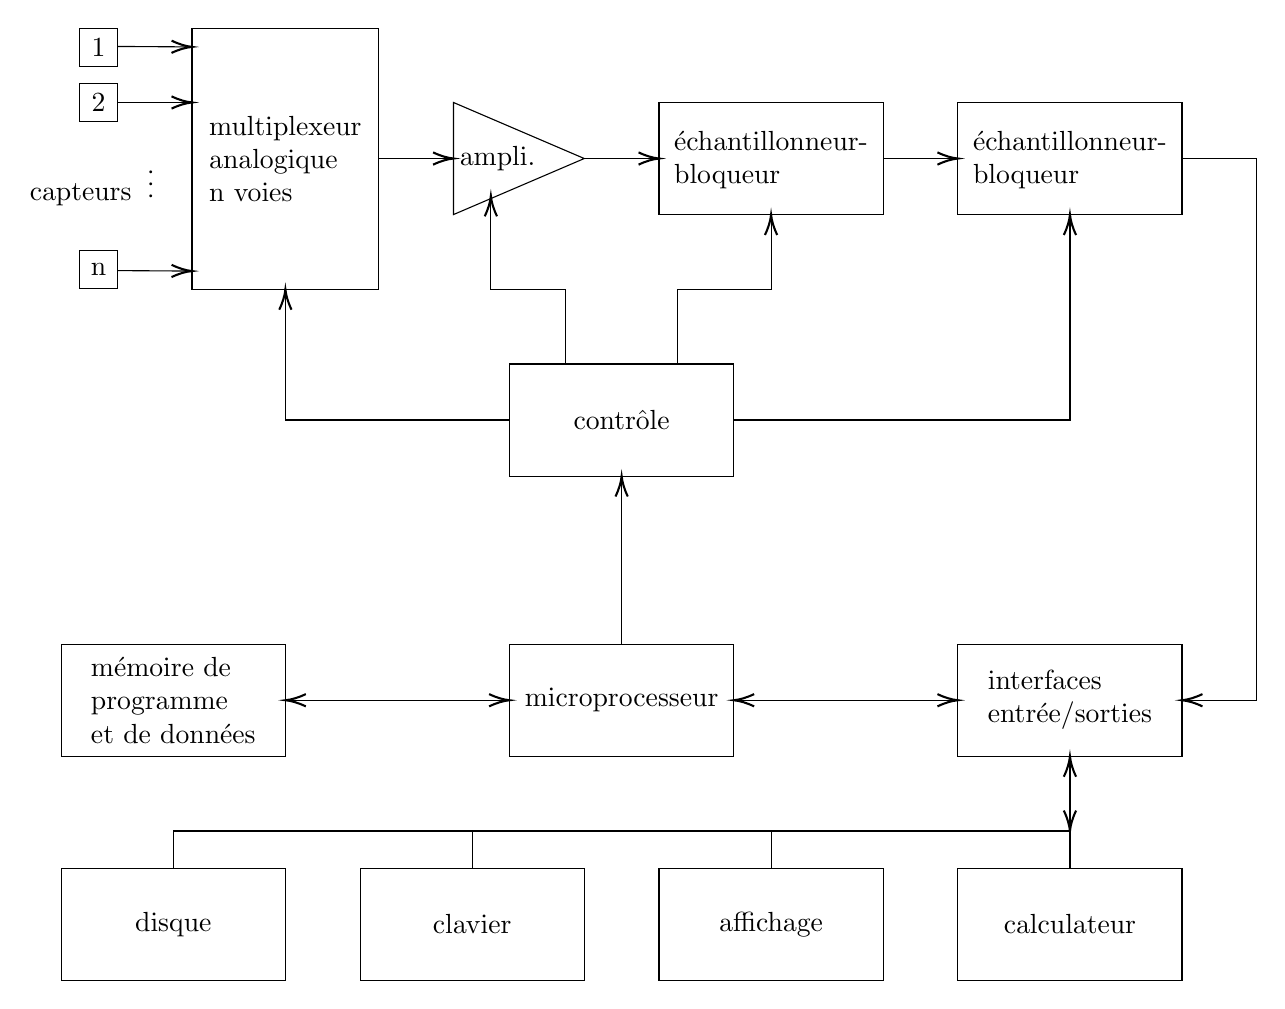
\begin{tikzpicture}[x=0.75pt,y=0.75pt,yscale=-0.9,xscale=0.9]
%uncomment if require: \path (0,542); %set diagram left start at 0, and has height of 542
%https://www.mathcha.io/editor/pJNZQf6yI3nHLEkz1QhWjMp2OT0JYgzyieBJNqK
%Flowchart: Process [id:dp6855416710808666] 
\draw   (110,10.25) -- (210,10.25) -- (210,150) -- (110,150) -- cycle ;
%Shape: Rectangle [id:dp004997227486996603] 
\draw   (50,10.25) -- (70,10.25) -- (70,30.75) -- (50,30.75) -- cycle ;
%Straight Lines [id:da4579113752456023] 
\draw    (70,20) -- (108,20.24) ;
\draw [shift={(110,20.25)}, rotate = 180.36] [color={rgb, 255:red, 0; green, 0; blue, 0 }  ][line width=0.75]    (10.93,-3.29) .. controls (6.95,-1.4) and (3.31,-0.3) .. (0,0) .. controls (3.31,0.3) and (6.95,1.4) .. (10.93,3.29)   ;
%Shape: Rectangle [id:dp6869458093862723] 
\draw   (50,39.75) -- (70,39.75) -- (70,60.25) -- (50,60.25) -- cycle ;
%Straight Lines [id:da4681455266308918] 
\draw    (70,50) -- (108,50) ;
\draw [shift={(110,50)}, rotate = 180] [color={rgb, 255:red, 0; green, 0; blue, 0 }  ][line width=0.75]    (10.93,-3.29) .. controls (6.95,-1.4) and (3.31,-0.3) .. (0,0) .. controls (3.31,0.3) and (6.95,1.4) .. (10.93,3.29)   ;
%Shape: Rectangle [id:dp45817791667488295] 
\draw   (50,129.25) -- (70,129.25) -- (70,149.75) -- (50,149.75) -- cycle ;
%Straight Lines [id:da30660098736037056] 
\draw    (70,140) -- (108,140.24) ;
\draw [shift={(110,140.25)}, rotate = 180.36] [color={rgb, 255:red, 0; green, 0; blue, 0 }  ][line width=0.75]    (10.93,-3.29) .. controls (6.95,-1.4) and (3.31,-0.3) .. (0,0) .. controls (3.31,0.3) and (6.95,1.4) .. (10.93,3.29)   ;
%Straight Lines [id:da6303825397789191] 
\draw    (210,80) -- (248,80) ;
\draw [shift={(250,80)}, rotate = 180] [color={rgb, 255:red, 0; green, 0; blue, 0 }  ][line width=0.75]    (10.93,-3.29) .. controls (6.95,-1.4) and (3.31,-0.3) .. (0,0) .. controls (3.31,0.3) and (6.95,1.4) .. (10.93,3.29)   ;
%Shape: Triangle [id:dp9560439033900896] 
\draw   (320,80) -- (250,110) -- (250,50) -- cycle ;
%Straight Lines [id:da5716448343517799] 
\draw    (320,80) -- (358,80) ;
\draw [shift={(360,80)}, rotate = 180] [color={rgb, 255:red, 0; green, 0; blue, 0 }  ][line width=0.75]    (10.93,-3.29) .. controls (6.95,-1.4) and (3.31,-0.3) .. (0,0) .. controls (3.31,0.3) and (6.95,1.4) .. (10.93,3.29)   ;
%Shape: Rectangle [id:dp5119568810350463] 
\draw   (360,50) -- (480,50) -- (480,110) -- (360,110) -- cycle ;
%Straight Lines [id:da4265953190983147] 
\draw    (480,80) -- (518,80) ;
\draw [shift={(520,80)}, rotate = 180] [color={rgb, 255:red, 0; green, 0; blue, 0 }  ][line width=0.75]    (10.93,-3.29) .. controls (6.95,-1.4) and (3.31,-0.3) .. (0,0) .. controls (3.31,0.3) and (6.95,1.4) .. (10.93,3.29)   ;
%Shape: Rectangle [id:dp7789656892769006] 
\draw   (520,50) -- (640,50) -- (640,110) -- (520,110) -- cycle ;
%Straight Lines [id:da93551183686321] 
\draw    (640,80) -- (680,80) -- (680,370) -- (642,370) ;
\draw [shift={(640,370)}, rotate = 360] [color={rgb, 255:red, 0; green, 0; blue, 0 }  ][line width=0.75]    (10.93,-3.29) .. controls (6.95,-1.4) and (3.31,-0.3) .. (0,0) .. controls (3.31,0.3) and (6.95,1.4) .. (10.93,3.29)   ;
%Shape: Rectangle [id:dp10942318417173202] 
\draw   (280,190) -- (400,190) -- (400,250) -- (280,250) -- cycle ;
%Straight Lines [id:da03354626475894362] 
\draw    (370,190) -- (370,150) -- (420,150) -- (420,112) ;
\draw [shift={(420,110)}, rotate = 450] [color={rgb, 255:red, 0; green, 0; blue, 0 }  ][line width=0.75]    (10.93,-3.29) .. controls (6.95,-1.4) and (3.31,-0.3) .. (0,0) .. controls (3.31,0.3) and (6.95,1.4) .. (10.93,3.29)   ;
%Straight Lines [id:da07083363231785789] 
\draw    (310,190) -- (310,150) -- (270,150) -- (270,102) ;
\draw [shift={(270,100)}, rotate = 450] [color={rgb, 255:red, 0; green, 0; blue, 0 }  ][line width=0.75]    (10.93,-3.29) .. controls (6.95,-1.4) and (3.31,-0.3) .. (0,0) .. controls (3.31,0.3) and (6.95,1.4) .. (10.93,3.29)   ;
%Straight Lines [id:da5566786216518755] 
\draw    (280,220) -- (160,220) -- (160,152) ;
\draw [shift={(160,150)}, rotate = 450] [color={rgb, 255:red, 0; green, 0; blue, 0 }  ][line width=0.75]    (10.93,-3.29) .. controls (6.95,-1.4) and (3.31,-0.3) .. (0,0) .. controls (3.31,0.3) and (6.95,1.4) .. (10.93,3.29)   ;
%Straight Lines [id:da44175483474459487] 
\draw    (400,220) -- (580,220) -- (580,112) ;
\draw [shift={(580,110)}, rotate = 450] [color={rgb, 255:red, 0; green, 0; blue, 0 }  ][line width=0.75]    (10.93,-3.29) .. controls (6.95,-1.4) and (3.31,-0.3) .. (0,0) .. controls (3.31,0.3) and (6.95,1.4) .. (10.93,3.29)   ;
%Straight Lines [id:da4950309462602226] 
\draw    (340,340) -- (340,252) ;
\draw [shift={(340,250)}, rotate = 450] [color={rgb, 255:red, 0; green, 0; blue, 0 }  ][line width=0.75]    (10.93,-3.29) .. controls (6.95,-1.4) and (3.31,-0.3) .. (0,0) .. controls (3.31,0.3) and (6.95,1.4) .. (10.93,3.29)   ;
%Shape: Rectangle [id:dp31894280515360696] 
\draw   (280,340) -- (400,340) -- (400,400) -- (280,400) -- cycle ;
%Shape: Rectangle [id:dp29748923859302145] 
\draw   (520,340) -- (640,340) -- (640,400) -- (520,400) -- cycle ;
%Straight Lines [id:da9319365647593406] 
\draw    (402,370) -- (518,370) ;
\draw [shift={(520,370)}, rotate = 180] [color={rgb, 255:red, 0; green, 0; blue, 0 }  ][line width=0.75]    (10.93,-3.29) .. controls (6.95,-1.4) and (3.31,-0.3) .. (0,0) .. controls (3.31,0.3) and (6.95,1.4) .. (10.93,3.29)   ;
\draw [shift={(400,370)}, rotate = 0] [color={rgb, 255:red, 0; green, 0; blue, 0 }  ][line width=0.75]    (10.93,-3.29) .. controls (6.95,-1.4) and (3.31,-0.3) .. (0,0) .. controls (3.31,0.3) and (6.95,1.4) .. (10.93,3.29)   ;
%Straight Lines [id:da5106166933182902] 
\draw    (162,370) -- (278,370) ;
\draw [shift={(280,370)}, rotate = 180] [color={rgb, 255:red, 0; green, 0; blue, 0 }  ][line width=0.75]    (10.93,-3.29) .. controls (6.95,-1.4) and (3.31,-0.3) .. (0,0) .. controls (3.31,0.3) and (6.95,1.4) .. (10.93,3.29)   ;
\draw [shift={(160,370)}, rotate = 0] [color={rgb, 255:red, 0; green, 0; blue, 0 }  ][line width=0.75]    (10.93,-3.29) .. controls (6.95,-1.4) and (3.31,-0.3) .. (0,0) .. controls (3.31,0.3) and (6.95,1.4) .. (10.93,3.29)   ;
%Shape: Rectangle [id:dp07598328049389613] 
\draw   (40,340) -- (160,340) -- (160,400) -- (40,400) -- cycle ;
%Straight Lines [id:da9982290158431298] 
\draw    (580,460) -- (580,440) -- (100,440) -- (100,460) ;
%Straight Lines [id:da9767066283683422] 
\draw    (260,440) -- (260,460) ;
%Straight Lines [id:da3569597647706805] 
\draw    (420,440) -- (420,460) ;
%Straight Lines [id:da26983482807496484] 
\draw    (580,402) -- (580,438) ;
\draw [shift={(580,440)}, rotate = 270] [color={rgb, 255:red, 0; green, 0; blue, 0 }  ][line width=0.75]    (10.93,-3.29) .. controls (6.95,-1.4) and (3.31,-0.3) .. (0,0) .. controls (3.31,0.3) and (6.95,1.4) .. (10.93,3.29)   ;
\draw [shift={(580,400)}, rotate = 90] [color={rgb, 255:red, 0; green, 0; blue, 0 }  ][line width=0.75]    (10.93,-3.29) .. controls (6.95,-1.4) and (3.31,-0.3) .. (0,0) .. controls (3.31,0.3) and (6.95,1.4) .. (10.93,3.29)   ;
%Shape: Rectangle [id:dp6771105282283583] 
\draw   (40,460) -- (160,460) -- (160,520) -- (40,520) -- cycle ;
%Shape: Rectangle [id:dp09474282891509045] 
\draw   (200,460) -- (320,460) -- (320,520) -- (200,520) -- cycle ;
%Shape: Rectangle [id:dp08838687884544572] 
\draw   (360,460) -- (480,460) -- (480,520) -- (360,520) -- cycle ;
%Shape: Rectangle [id:dp49628749586658394] 
\draw   (520,460) -- (640,460) -- (640,520) -- (520,520) -- cycle ;

% Text Node
\draw (160,80.13) node   [align=left] {multiplexeur\\analogique\\n voies};
% Text Node
\draw (60,20.5) node   [align=left] {1};
% Text Node
\draw (60,50) node   [align=left] {2};
% Text Node
\draw (60,139.5) node   [align=left] {n};
% Text Node
\draw (88,95) node  [rotate=-90] [align=left] {\ldots};
% Text Node
\draw (79,99.5) node [anchor=east] [inner sep=0.75pt]   [align=left] {capteurs};
% Text Node
\draw (252,72) node [anchor=north west][inner sep=0.75pt]   [align=left] {ampli.};
% Text Node
\draw (420,81) node   [align=left] {échantillonneur-\\bloqueur};
% Text Node
\draw (580,81) node   [align=left] {échantillonneur-\\bloqueur};
% Text Node
\draw (340,220) node   [align=left] {contrôle};
% Text Node
\draw (340,370) node   [align=left] {microprocesseur};
% Text Node
\draw (580,370) node   [align=left] {interfaces\\entrée/sorties};
% Text Node
\draw (100,370) node   [align=left] {mémoire de \\programme \\et de données};
% Text Node
\draw (100,490) node   [align=left] {disque};
% Text Node
\draw (260,490) node   [align=left] {clavier};
% Text Node
\draw (420,490) node   [align=left] {affichage};
% Text Node
\draw (580,490) node   [align=left] {calculateur};


\end{tikzpicture}
\end{figure}

Le calculateur associée à la chaine de mesure des fonctions importantes dans la chaine de mesure, elles sont regroupées dans deux catégories :
\begin{itemize}
\item gestion de l'acquisition\,;
\item traitement du signal requis par la précision et la nature de l'information cherchée.
\end{itemize}

Il gère la chaine d'acquisition en délivrant des séquences de signaux de commande. Ceux-ci vont activer de façon ordonnée les dispositifs prévus pour obtenir la valeur du mesurande $m$ :
\begin{enumerate}
\item sélection d'une voie d'entrée par envoie d'adresse au multiplexeur\,;
\item fixation du gain de l'amplificateur programmable\,;
\item échantillonnage puis blocage du signal\,;
\item déclenchement de la conversion analogique-numérique\,;
\item lecture de la donnée numérique à la réception du signal de fin de conversion délivré par le convertisseur analogique-numérique.
\end{enumerate}

En aval de la chaine d'acquisition, le calculateur gère également les périphériques d'entrée-sortie :
\begin{itemize}
\item clavier permettant l'introduction, pour prise en compte par la chaine, d'ordres et de modifications de paramètres de mesure\,;
\item mémoire de masse pour l'archivage des mesures\,;
\item affichage du résultat de la mesure en cours.
\end{itemize}

Les calculateurs permettent aussi d'effectuer des opérations mathématiques sur le signal capté et numérisé :
\begin{itemize}
\item correction du signal reçu\,;
	\begin{itemize}
	\item correction des dérives de zéro et de sensibilité causées par les grandeurs d'influences (en particulier les températures)\,;
	\item correction de la \emph{non-linéarité} des capteurs afin d'obtenir une donnée de sortie proportionnelle au mesurande\,;
	\end{itemize}
\item analyse du signal corrigé.
\end{itemize}



%\end{document}


	%--------------------------------------
%ELECTROTECHNIQUE - SCHEMA DE LIAISON A LA TERRE
%--------------------------------------

%utiliser les environnement \begin{comment} \end{comment} pour mettre en commentaire le préambule une fois la programmation appelée dans le document maître (!ne pas oublier de mettre en commentaire \end{document}!)

\begin{comment}

\documentclass[a4paper, 11pt, twoside, fleqn]{memoir}

\usepackage{AOCDTF}

\marqueurchapitre

%--------------------------------------
%corps du document
%--------------------------------------

\begin{document} %corps du document
	\openleft %début de chapitre à gauche

\end{comment}

\chapter{Schéma Terre-Terre}
\ChapFrame

\section{Caractéristiques générales}

\begin{definition}[Schéma TT]
Schéma de liaison à la terre dans lequel :
\begin{description}
\item[Neutre :] relié à la terre\,;
\item[Masse :] reliées à la terre.
\end{description}
\end{definition}

Dans le SLT TT, le point neutre du transformateur HT/BT (point commun) est relié à la terre via la \emph{prise de terre du neutre} \Circled{1}. Cette liaison présente une certaine résistance, la \emph{résistance de la prise de terre du neutre} $R_B$ \Circled{2}. Sa mise en \oe{}uvre est à charge du fournisseur d'électricité et sa résistance globale doit être inférieure ou égale à \SI{15}{\ohm} \supercite{NF:C13-100-2015}.\\
Les masses sont quant à elles reliées à la terre via la \emph{prise de terre de l'installation électrique} \Circled{3}, qui présente aussi une certaine résistance, la \emph{résistance de la prise de terre de l'installation électrique} $R_A$ \Circled{4}. Sa mise en \oe{}uvre est à charge du propriétaire de l'installation (voir \superref{subsec:prise_terre_installation_electrique}).\\ 

\section{Schémas de principe}

\begin{figure}[h]
\caption{Installation Terre-Terre}
\begin{subfigure}[t]{0.49\linewidth}
%--------------------------------------
%ELECTROTECHNIQUE - SCHEMA DE LIAISON A LA TERRE
%--------------------------------------

%utiliser les environnement \begin{comment} \end{comment} pour mettre en commentaire le préambule une fois la programmation appelée dans le document maître (!ne pas oublier de mettre en commentaire \end{document}!)

\begin{comment}

\documentclass[a4paper, 11pt, twoside, fleqn]{memoir}

\usepackage{AOCDTF}

\marqueurchapitre 

%lien d'édition des figures Tikz sur le site mathcha.io (rajouter le lien d'une modification effectuée sur la figure tikz avec le nom du modificateur car il n'y a qu'un lien par compte)

%lien mathcha Bruno Douchy : https://www.mathcha.io/editor/NXxYZiYwiOph2ogqzlc1q32LohL4j2ZYCPD09q3

%--------------------------------------
%corps du document
%--------------------------------------

\begin{document} %corps du document
	\openleft %début de chapitre à gauche

\end{comment}







% Pattern Info
 
\tikzset{
pattern size/.store in=\mcSize, 
pattern size = 5pt,
pattern thickness/.store in=\mcThickness, 
pattern thickness = 0.3pt,
pattern radius/.store in=\mcRadius, 
pattern radius = 1pt}
\makeatletter
\pgfutil@ifundefined{pgf@pattern@name@_vicu0hcww}{
\pgfdeclarepatternformonly[\mcThickness,\mcSize]{_vicu0hcww}
{\pgfqpoint{0pt}{0pt}}
{\pgfpoint{\mcSize+\mcThickness}{\mcSize+\mcThickness}}
{\pgfpoint{\mcSize}{\mcSize}}
{
\pgfsetcolor{\tikz@pattern@color}
\pgfsetlinewidth{\mcThickness}
\pgfpathmoveto{\pgfqpoint{0pt}{0pt}}
\pgfpathlineto{\pgfpoint{\mcSize+\mcThickness}{\mcSize+\mcThickness}}
\pgfusepath{stroke}
}}
\makeatother
\tikzset{every picture/.style={line width=0.5pt}} %set default line width to 0.75pt        

\begin{tikzpicture}[x=0.75pt,y=0.75pt,yscale=-0.6,xscale=0.6]
%uncomment if require: \path (0,293); %set diagram left start at 0, and has height of 293

%Straight Lines [id:da5569675718372048] 
\draw [color={rgb, 255:red, 248; green, 231; blue, 28 }  ,draw opacity=1 ]   (87.5,222.5) -- (87.5,252.5) ;
%Straight Lines [id:da8030717374799764] 
\draw [color={rgb, 255:red, 248; green, 231; blue, 28 }  ,draw opacity=1 ]   (240,135) -- (225,135) -- (225,182.5) ;
%Straight Lines [id:da7894327394796508] 
\draw    (120,35) -- (162.5,35) ;
%Straight Lines [id:da6671442734999171] 
\draw [color={rgb, 255:red, 139; green, 87; blue, 42 }  ,draw opacity=1 ]   (112.5,15) -- (162.5,15) ;
%Straight Lines [id:da16231501811449245] 
\draw [color={rgb, 255:red, 155; green, 155; blue, 155 }  ,draw opacity=1 ]   (112.5,55) -- (162.5,55) ;
%Straight Lines [id:da04476213273823848] 
\draw [color={rgb, 255:red, 74; green, 144; blue, 226 }  ,draw opacity=1 ]   (87.5,75) -- (162.5,75) ;
%Straight Lines [id:da2559241348150122] 
\draw [color={rgb, 255:red, 248; green, 231; blue, 28 }  ,draw opacity=1 ]   (95.5,35) -- (87.5,75) -- (87.5,182.5) ;
%Straight Lines [id:da8531850209376354] 
\draw [color={rgb, 255:red, 126; green, 211; blue, 33 }  ,draw opacity=1 ] [dash pattern={on 4.5pt off 4.5pt}]  (95.5,35) -- (87.5,75) -- (87.5,182.5) ;
%Shape: Circle [id:dp47194931654687355] 
\draw  [fill={rgb, 255:red, 0; green, 0; blue, 0 }  ,fill opacity=1 ] (85,75) .. controls (85,73.62) and (86.12,72.5) .. (87.5,72.5) .. controls (88.88,72.5) and (90,73.62) .. (90,75) .. controls (90,76.38) and (88.88,77.5) .. (87.5,77.5) .. controls (86.12,77.5) and (85,76.38) .. (85,75) -- cycle ;
%Straight Lines [id:da12418542898468488] 
\draw    (202.5,35) -- (460,35) ;
%Straight Lines [id:da892541875072728] 
\draw [color={rgb, 255:red, 139; green, 87; blue, 42 }  ,draw opacity=1 ]   (202.5,15) -- (460,15) ;
%Straight Lines [id:da742409178470536] 
\draw [color={rgb, 255:red, 155; green, 155; blue, 155 }  ,draw opacity=1 ]   (202.5,55) -- (460,55) ;
%Straight Lines [id:da856527021466942] 
\draw [color={rgb, 255:red, 74; green, 144; blue, 226 }  ,draw opacity=1 ]   (202.5,75) -- (462.5,75) ;
%Shape: Path Data [id:dp19593575615064884] 
\draw   (112.5,55) .. controls (112.5,56.38) and (111.38,57.5) .. (110,57.5) .. controls (109.29,57.5) and (108.65,57.2) .. (108.19,56.72) .. controls (102.81,61.85) and (95.52,65) .. (87.5,65) .. controls (70.93,65) and (57.5,51.57) .. (57.5,35) .. controls (57.5,18.43) and (70.93,5) .. (87.5,5) .. controls (95.52,5) and (102.81,8.15) .. (108.19,13.28) .. controls (108.65,12.8) and (109.29,12.5) .. (110,12.5) .. controls (111.38,12.5) and (112.5,13.62) .. (112.5,15) .. controls (112.5,15.82) and (112.11,16.54) .. (111.5,17) .. controls (114.8,21.39) and (116.92,26.71) .. (117.4,32.5) .. controls (117.43,32.5) and (117.47,32.5) .. (117.5,32.5) .. controls (118.88,32.5) and (120,33.62) .. (120,35) .. controls (120,36.38) and (118.88,37.5) .. (117.5,37.5) .. controls (117.47,37.5) and (117.43,37.5) .. (117.4,37.5) .. controls (116.92,43.29) and (114.8,48.61) .. (111.5,53) .. controls (112.11,53.46) and (112.5,54.18) .. (112.5,55) -- cycle ;
%Shape: Circle [id:dp7917428977896803] 
\draw   (17.5,35) .. controls (17.5,18.43) and (30.93,5) .. (47.5,5) .. controls (64.07,5) and (77.5,18.43) .. (77.5,35) .. controls (77.5,51.57) and (64.07,65) .. (47.5,65) .. controls (30.93,65) and (17.5,51.57) .. (17.5,35) -- cycle ;
%Shape: Triangle [id:dp8517252312032021] 
\draw   (40,25) -- (30,42.5) -- (50,42.5) -- cycle ;
%Shape: Star [id:dp07223973274580164] 
\draw   (106.75,35) -- (95.5,35) -- (89.88,44.81) -- (95.5,35) -- (89.88,25.19) -- (95.5,35) -- cycle ;
%Shape: Circle [id:dp389562574882782] 
\draw   (107.5,15) .. controls (107.5,13.62) and (108.62,12.5) .. (110,12.5) .. controls (111.38,12.5) and (112.5,13.62) .. (112.5,15) .. controls (112.5,16.38) and (111.38,17.5) .. (110,17.5) .. controls (108.62,17.5) and (107.5,16.38) .. (107.5,15) -- cycle ;
%Shape: Circle [id:dp684435310402229] 
\draw   (114.9,35) .. controls (114.9,33.62) and (116.02,32.5) .. (117.4,32.5) .. controls (118.78,32.5) and (119.9,33.62) .. (119.9,35) .. controls (119.9,36.38) and (118.78,37.5) .. (117.4,37.5) .. controls (116.02,37.5) and (114.9,36.38) .. (114.9,35) -- cycle ;
%Shape: Circle [id:dp060632852060490405] 
\draw   (107.5,55) .. controls (107.5,53.62) and (108.62,52.5) .. (110,52.5) .. controls (111.38,52.5) and (112.5,53.62) .. (112.5,55) .. controls (112.5,56.38) and (111.38,57.5) .. (110,57.5) .. controls (108.62,57.5) and (107.5,56.38) .. (107.5,55) -- cycle ;

%Straight Lines [id:da9609078171715071] 
\draw [color={rgb, 255:red, 74; green, 144; blue, 226 }  ,draw opacity=1 ]   (292.5,112.5) -- (292.5,77.5) ;
%Straight Lines [id:da90253425713718] 
\draw [color={rgb, 255:red, 139; green, 87; blue, 42 }  ,draw opacity=1 ]   (252.5,112.5) -- (252.5,17.5) ;
%Straight Lines [id:da41836049222392757] 
\draw [color={rgb, 255:red, 139; green, 87; blue, 42 }  ,draw opacity=1 ]   (252.5,130) -- (252.5,117.5) ;
%Straight Lines [id:da8111963186758367] 
\draw [color={rgb, 255:red, 74; green, 144; blue, 226 }  ,draw opacity=1 ]   (292.5,130.5) -- (292.5,117.5) ;
%Straight Lines [id:da7572420158424509] 
\draw    (45,232.5) -- (460,232.5) ;
%Shape: Rectangle [id:dp18411529638071378] 
\draw  [draw opacity=0][pattern=_vicu0hcww,pattern size=6pt,pattern thickness=0.75pt,pattern radius=0pt, pattern color={rgb, 255:red, 0; green, 0; blue, 0}][line width=0.75]  (45,232.5) -- (460,232.5) -- (460,247.5) -- (45,247.5) -- cycle ;
%Straight Lines [id:da03392621889598857] 
\draw [color={rgb, 255:red, 126; green, 211; blue, 33 }  ,draw opacity=1 ] [dash pattern={on 4.5pt off 4.5pt}]  (240,135) -- (225,135) -- (225,182.5) ;
%Straight Lines [id:da20553450120643402] 
\draw    (87.5,252.5) -- (87.5,267.5) ;
%Straight Lines [id:da9544857402361856] 
\draw    (77.5,267.5) -- (97.5,267.5) ;
%Straight Lines [id:da6836120465702779] 
\draw    (80,272.5) -- (95,272.5) ;
%Straight Lines [id:da5098314930953095] 
\draw    (82.5,277.5) -- (92.5,277.5) ;

%Straight Lines [id:da14748133582745382] 
\draw [color={rgb, 255:red, 126; green, 211; blue, 33 }  ,draw opacity=1 ] [dash pattern={on 4.5pt off 4.5pt}]  (87.5,222.5) -- (87.5,252.5) ;
%Straight Lines [id:da07788601461052536] 
\draw [color={rgb, 255:red, 248; green, 231; blue, 28 }  ,draw opacity=1 ]   (225,222.5) -- (225,247.5) ;
%Straight Lines [id:da077984621762062] 
\draw    (225,247.5) -- (225,262.5) ;
%Straight Lines [id:da01964510614427828] 
\draw    (215,262.5) -- (235,262.5) ;
%Straight Lines [id:da29977229045078546] 
\draw    (217.5,267.5) -- (232.5,267.5) ;
%Straight Lines [id:da6901624132325382] 
\draw    (220,272.5) -- (230,272.5) ;

%Straight Lines [id:da32226465457516273] 
\draw [color={rgb, 255:red, 126; green, 211; blue, 33 }  ,draw opacity=1 ] [dash pattern={on 4.5pt off 4.5pt}]  (225,222.5) -- (225,247.5) ;
%Straight Lines [id:da2085284947671493] 
\draw    (287.5,130) -- (292.5,130) ;
%Shape: Rectangle [id:dp3078829888067669] 
\draw   (257.5,125) -- (287.5,125) -- (287.5,135) -- (257.5,135) -- cycle ;
%Straight Lines [id:da04494606262403944] 
\draw    (252.5,130) -- (257.5,130) ;

%Straight Lines [id:da05615200975856005] 
\draw    (87.5,217.5) -- (87.5,222.5) ;
%Shape: Rectangle [id:dp9785804407278047] 
\draw   (92.5,187.5) -- (92.5,217.5) -- (82.5,217.5) -- (82.5,187.5) -- cycle ;
%Straight Lines [id:da7148865545802072] 
\draw    (87.5,182.5) -- (87.5,187.5) ;

%Straight Lines [id:da44059104169861363] 
\draw    (225,217.5) -- (225,222.5) ;
%Shape: Rectangle [id:dp6614259081430341] 
\draw   (230,187.5) -- (230,217.5) -- (220,217.5) -- (220,187.5) -- cycle ;
%Straight Lines [id:da7546178831476872] 
\draw    (225,182.5) -- (225,187.5) ;

%Straight Lines [id:da5381487672364753] 
\draw    (170,87.5) -- (192.5,75) -- (212.5,75) ;
%Shape: Circle [id:dp5063041840027898] 
\draw   (172.5,73) .. controls (171.4,73) and (170.5,73.9) .. (170.5,75) .. controls (170.5,76.1) and (171.4,77) .. (172.5,77) .. controls (173.6,77) and (174.5,76.1) .. (174.5,75) .. controls (174.5,73.9) and (173.6,73) .. (172.5,73) -- cycle ;
%Straight Lines [id:da016267948872827898] 
\draw    (170.5,75) -- (162.5,75) ;
%Rounded Rect [id:dp6441566231879102] 
\draw   (202.5,80) .. controls (201.12,80) and (200,78.88) .. (200,77.5) -- (200,12.5) .. controls (200,11.12) and (201.12,10) .. (202.5,10) -- (202.5,10) .. controls (203.88,10) and (205,11.12) .. (205,12.5) -- (205,77.5) .. controls (205,78.88) and (203.88,80) .. (202.5,80) -- cycle ;
%Straight Lines [id:da9573520376137438] 
\draw  [dash pattern={on 2.25pt off 2.25pt}]  (182.25,20.25) -- (182.5,85) -- (202.5,85) -- (202.5,80) ;
%Straight Lines [id:da9709025205318027] 
\draw    (170,67.5) -- (192.5,55) -- (212.5,55) ;
%Shape: Circle [id:dp9923026286446914] 
\draw   (172.5,53) .. controls (171.4,53) and (170.5,53.9) .. (170.5,55) .. controls (170.5,56.1) and (171.4,57) .. (172.5,57) .. controls (173.6,57) and (174.5,56.1) .. (174.5,55) .. controls (174.5,53.9) and (173.6,53) .. (172.5,53) -- cycle ;
%Straight Lines [id:da6982236178440787] 
\draw    (170.5,55) -- (162.5,55) ;
%Straight Lines [id:da967051244304329] 
\draw    (170,47.5) -- (192.5,35) -- (212.5,35) ;
%Shape: Circle [id:dp1005994292384611] 
\draw   (172.5,33) .. controls (171.4,33) and (170.5,33.9) .. (170.5,35) .. controls (170.5,36.1) and (171.4,37) .. (172.5,37) .. controls (173.6,37) and (174.5,36.1) .. (174.5,35) .. controls (174.5,33.9) and (173.6,33) .. (172.5,33) -- cycle ;
%Straight Lines [id:da8130885764394731] 
\draw    (170.5,35) -- (162.5,35) ;
%Straight Lines [id:da40883431078631327] 
\draw    (170,27.5) -- (192.5,15) -- (212.5,15) ;
%Shape: Circle [id:dp937545867990687] 
\draw   (172.5,13) .. controls (171.4,13) and (170.5,13.9) .. (170.5,15) .. controls (170.5,16.1) and (171.4,17) .. (172.5,17) .. controls (173.6,17) and (174.5,16.1) .. (174.5,15) .. controls (174.5,13.9) and (173.6,13) .. (172.5,13) -- cycle ;
%Straight Lines [id:da3794342958375365] 
\draw    (170.5,15) -- (162.5,15) ;

%Straight Lines [id:da5459132304975308] 
\draw [color={rgb, 255:red, 248; green, 231; blue, 28 }  ,draw opacity=1 ]   (325,135) -- (310,135) -- (310,155) -- (227.5,155.25) ;
%Straight Lines [id:da9739292778940422] 
\draw [color={rgb, 255:red, 74; green, 144; blue, 226 }  ,draw opacity=1 ]   (377.5,112.5) -- (377.5,77.5) ;
%Straight Lines [id:da5586324527914077] 
\draw [color={rgb, 255:red, 139; green, 87; blue, 42 }  ,draw opacity=1 ]   (337.5,112.5) -- (337.5,17.5) ;
%Straight Lines [id:da43861605672672455] 
\draw [color={rgb, 255:red, 139; green, 87; blue, 42 }  ,draw opacity=1 ]   (337.5,130) -- (337.5,117.5) ;
%Straight Lines [id:da22845927200448446] 
\draw [color={rgb, 255:red, 74; green, 144; blue, 226 }  ,draw opacity=1 ]   (377.5,130.5) -- (377.5,117.5) ;
%Straight Lines [id:da6117495087264712] 
\draw [color={rgb, 255:red, 126; green, 211; blue, 33 }  ,draw opacity=1 ] [dash pattern={on 4.5pt off 4.5pt}]  (325,135) -- (310,135) -- (310,155) -- (227.5,155.25) ;
%Straight Lines [id:da7106863605150712] 
\draw    (372.5,130) -- (377.5,130) ;
%Shape: Rectangle [id:dp04624338825083918] 
\draw   (342.5,125) -- (372.5,125) -- (372.5,135) -- (342.5,135) -- cycle ;
%Straight Lines [id:da8671552569910891] 
\draw    (337.5,130) -- (342.5,130) ;

%Straight Lines [id:da03248547821407621] 
\draw [color={rgb, 255:red, 248; green, 231; blue, 28 }  ,draw opacity=1 ]   (410,135) -- (395,135) -- (395,170) -- (225,170) ;
%Straight Lines [id:da6602842298062329] 
\draw [color={rgb, 255:red, 74; green, 144; blue, 226 }  ,draw opacity=1 ]   (462.5,112.5) -- (462.5,77.5) ;
%Straight Lines [id:da38294124111277295] 
\draw [color={rgb, 255:red, 139; green, 87; blue, 42 }  ,draw opacity=1 ]   (422.5,112.5) -- (422.5,17.5) ;
%Straight Lines [id:da875801079628449] 
\draw [color={rgb, 255:red, 139; green, 87; blue, 42 }  ,draw opacity=1 ]   (422.5,130) -- (422.5,117.5) ;
%Straight Lines [id:da6549070297454946] 
\draw [color={rgb, 255:red, 74; green, 144; blue, 226 }  ,draw opacity=1 ]   (462.5,130.5) -- (462.5,117.5) ;
%Straight Lines [id:da32714750122574565] 
\draw [color={rgb, 255:red, 126; green, 211; blue, 33 }  ,draw opacity=1 ] [dash pattern={on 4.5pt off 4.5pt}]  (410,135) -- (395,135) -- (395,170) -- (225,170) ;
%Straight Lines [id:da286106121704247] 
\draw    (457.5,130) -- (462.5,130) ;
%Shape: Rectangle [id:dp4701657834308206] 
\draw   (427.5,125) -- (457.5,125) -- (457.5,135) -- (427.5,135) -- cycle ;
%Straight Lines [id:da5463375839867839] 
\draw    (422.5,130) -- (427.5,130) ;

%Shape: Circle [id:dp19173673105912947] 
\draw  [fill={rgb, 255:red, 0; green, 0; blue, 0 }  ,fill opacity=1 ] (375,75) .. controls (375,73.62) and (376.12,72.5) .. (377.5,72.5) .. controls (378.88,72.5) and (380,73.62) .. (380,75) .. controls (380,76.38) and (378.88,77.5) .. (377.5,77.5) .. controls (376.12,77.5) and (375,76.38) .. (375,75) -- cycle ;
%Shape: Circle [id:dp3455768921834108] 
\draw  [fill={rgb, 255:red, 0; green, 0; blue, 0 }  ,fill opacity=1 ] (460,75) .. controls (460,73.62) and (461.12,72.5) .. (462.5,72.5) .. controls (463.88,72.5) and (465,73.62) .. (465,75) .. controls (465,76.38) and (463.88,77.5) .. (462.5,77.5) .. controls (461.12,77.5) and (460,76.38) .. (460,75) -- cycle ;
%Shape: Circle [id:dp6902292346661852] 
\draw  [fill={rgb, 255:red, 0; green, 0; blue, 0 }  ,fill opacity=1 ] (335,15) .. controls (335,13.62) and (336.12,12.5) .. (337.5,12.5) .. controls (338.88,12.5) and (340,13.62) .. (340,15) .. controls (340,16.38) and (338.88,17.5) .. (337.5,17.5) .. controls (336.12,17.5) and (335,16.38) .. (335,15) -- cycle ;
%Shape: Circle [id:dp7821656065480904] 
\draw  [fill={rgb, 255:red, 0; green, 0; blue, 0 }  ,fill opacity=1 ] (420,15) .. controls (420,13.62) and (421.12,12.5) .. (422.5,12.5) .. controls (423.88,12.5) and (425,13.62) .. (425,15) .. controls (425,16.38) and (423.88,17.5) .. (422.5,17.5) .. controls (421.12,17.5) and (420,16.38) .. (420,15) -- cycle ;
%Shape: Circle [id:dp9145976676566879] 
\draw  [fill={rgb, 255:red, 0; green, 0; blue, 0 }  ,fill opacity=1 ] (222.5,170) .. controls (222.5,168.62) and (223.62,167.5) .. (225,167.5) .. controls (226.38,167.5) and (227.5,168.62) .. (227.5,170) .. controls (227.5,171.38) and (226.38,172.5) .. (225,172.5) .. controls (223.62,172.5) and (222.5,171.38) .. (222.5,170) -- cycle ;
%Shape: Circle [id:dp4159197044363645] 
\draw  [fill={rgb, 255:red, 0; green, 0; blue, 0 }  ,fill opacity=1 ] (290,75) .. controls (290,73.62) and (291.12,72.5) .. (292.5,72.5) .. controls (293.88,72.5) and (295,73.62) .. (295,75) .. controls (295,76.38) and (293.88,77.5) .. (292.5,77.5) .. controls (291.12,77.5) and (290,76.38) .. (290,75) -- cycle ;
%Shape: Circle [id:dp7956802061064191] 
\draw  [fill={rgb, 255:red, 0; green, 0; blue, 0 }  ,fill opacity=1 ] (250,15) .. controls (250,13.62) and (251.12,12.5) .. (252.5,12.5) .. controls (253.88,12.5) and (255,13.62) .. (255,15) .. controls (255,16.38) and (253.88,17.5) .. (252.5,17.5) .. controls (251.12,17.5) and (250,16.38) .. (250,15) -- cycle ;
%Shape: Circle [id:dp3974117127226756] 
\draw  [fill={rgb, 255:red, 0; green, 0; blue, 0 }  ,fill opacity=1 ] (222.5,155.25) .. controls (222.5,153.87) and (223.62,152.75) .. (225,152.75) .. controls (226.38,152.75) and (227.5,153.87) .. (227.5,155.25) .. controls (227.5,156.63) and (226.38,157.75) .. (225,157.75) .. controls (223.62,157.75) and (222.5,156.63) .. (222.5,155.25) -- cycle ;
%Straight Lines [id:da4669926547480553] 
\draw    (70,152.5) -- (81.83,185.62) ;
\draw [shift={(82.5,187.5)}, rotate = 250.35] [color={rgb, 255:red, 0; green, 0; blue, 0 }  ][line width=0.75]    (10.93,-3.29) .. controls (6.95,-1.4) and (3.31,-0.3) .. (0,0) .. controls (3.31,0.3) and (6.95,1.4) .. (10.93,3.29)   ;
%Straight Lines [id:da335578810680045] 
\draw    (142.5,212.5) -- (96.38,261.05) ;
\draw [shift={(95,262.5)}, rotate = 313.53] [color={rgb, 255:red, 0; green, 0; blue, 0 }  ][line width=0.75]    (10.93,-3.29) .. controls (6.95,-1.4) and (3.31,-0.3) .. (0,0) .. controls (3.31,0.3) and (6.95,1.4) .. (10.93,3.29)   ;
%Straight Lines [id:da1248544792034546] 
\draw    (287.5,215) -- (236.55,256.24) ;
\draw [shift={(235,257.5)}, rotate = 321.01] [color={rgb, 255:red, 0; green, 0; blue, 0 }  ][line width=0.75]    (10.93,-3.29) .. controls (6.95,-1.4) and (3.31,-0.3) .. (0,0) .. controls (3.31,0.3) and (6.95,1.4) .. (10.93,3.29)   ;
%Straight Lines [id:da35708867716754655] 
\draw    (185,132.5) -- (218.93,185.81) ;
\draw [shift={(220,187.5)}, rotate = 237.53] [color={rgb, 255:red, 0; green, 0; blue, 0 }  ][line width=0.75]    (10.93,-3.29) .. controls (6.95,-1.4) and (3.31,-0.3) .. (0,0) .. controls (3.31,0.3) and (6.95,1.4) .. (10.93,3.29)   ;
%Shape: Rectangle [id:dp9097154918949548] 
\draw  [thin, dash pattern={on 2.25pt off 2.25pt on 1pt off 2.25pt}] (242.5,115) -- (302.5,115) -- (302.5,145) -- (242.5,145) -- cycle ;
%Shape: Circle [id:dp2975569828456256] 
\draw  [fill={rgb, 255:red, 255; green, 255; blue, 255 }  ,fill opacity=1 ] (240,135) .. controls (240,133.62) and (241.12,132.5) .. (242.5,132.5) .. controls (243.88,132.5) and (245,133.62) .. (245,135) .. controls (245,136.38) and (243.88,137.5) .. (242.5,137.5) .. controls (241.12,137.5) and (240,136.38) .. (240,135) -- cycle ;
%Shape: Circle [id:dp41677745800182897] 
\draw  [fill={rgb, 255:red, 255; green, 255; blue, 255 }  ,fill opacity=1 ] (250,115) .. controls (250,113.62) and (251.12,112.5) .. (252.5,112.5) .. controls (253.88,112.5) and (255,113.62) .. (255,115) .. controls (255,116.38) and (253.88,117.5) .. (252.5,117.5) .. controls (251.12,117.5) and (250,116.38) .. (250,115) -- cycle ;
%Shape: Circle [id:dp14395725895377898] 
\draw  [fill={rgb, 255:red, 255; green, 255; blue, 255 }  ,fill opacity=1 ] (290,115) .. controls (290,113.62) and (291.12,112.5) .. (292.5,112.5) .. controls (293.88,112.5) and (295,113.62) .. (295,115) .. controls (295,116.38) and (293.88,117.5) .. (292.5,117.5) .. controls (291.12,117.5) and (290,116.38) .. (290,115) -- cycle ;
%Shape: Rectangle [id:dp5120060222437024] 
\draw  [thin, dash pattern={on 2.25pt off 2.25pt on 1pt off 2.25pt}] (327.5,115) -- (387.5,115) -- (387.5,145) -- (327.5,145) -- cycle ;
%Shape: Circle [id:dp7511256761018086] 
\draw  [fill={rgb, 255:red, 255; green, 255; blue, 255 }  ,fill opacity=1 ] (325,135) .. controls (325,133.62) and (326.12,132.5) .. (327.5,132.5) .. controls (328.88,132.5) and (330,133.62) .. (330,135) .. controls (330,136.38) and (328.88,137.5) .. (327.5,137.5) .. controls (326.12,137.5) and (325,136.38) .. (325,135) -- cycle ;
%Shape: Circle [id:dp901649704749009] 
\draw  [fill={rgb, 255:red, 255; green, 255; blue, 255 }  ,fill opacity=1 ] (335,115) .. controls (335,113.62) and (336.12,112.5) .. (337.5,112.5) .. controls (338.88,112.5) and (340,113.62) .. (340,115) .. controls (340,116.38) and (338.88,117.5) .. (337.5,117.5) .. controls (336.12,117.5) and (335,116.38) .. (335,115) -- cycle ;
%Shape: Circle [id:dp03510351381962351] 
\draw  [fill={rgb, 255:red, 255; green, 255; blue, 255 }  ,fill opacity=1 ] (375,115) .. controls (375,113.62) and (376.12,112.5) .. (377.5,112.5) .. controls (378.88,112.5) and (380,113.62) .. (380,115) .. controls (380,116.38) and (378.88,117.5) .. (377.5,117.5) .. controls (376.12,117.5) and (375,116.38) .. (375,115) -- cycle ;
%Shape: Rectangle [id:dp9758492438120955] 
\draw  [thin, dash pattern={on 2.25pt off 2.25pt on 1pt off 2.25pt}] (412.5,115) -- (472.5,115) -- (472.5,145) -- (412.5,145) -- cycle ;
%Shape: Circle [id:dp6388682497746971] 
\draw  [fill={rgb, 255:red, 255; green, 255; blue, 255 }  ,fill opacity=1 ] (410,135) .. controls (410,133.62) and (411.12,132.5) .. (412.5,132.5) .. controls (413.88,132.5) and (415,133.62) .. (415,135) .. controls (415,136.38) and (413.88,137.5) .. (412.5,137.5) .. controls (411.12,137.5) and (410,136.38) .. (410,135) -- cycle ;
%Shape: Circle [id:dp8952907004738548] 
\draw  [fill={rgb, 255:red, 255; green, 255; blue, 255 }  ,fill opacity=1 ] (420,115) .. controls (420,113.62) and (421.12,112.5) .. (422.5,112.5) .. controls (423.88,112.5) and (425,113.62) .. (425,115) .. controls (425,116.38) and (423.88,117.5) .. (422.5,117.5) .. controls (421.12,117.5) and (420,116.38) .. (420,115) -- cycle ;
%Shape: Circle [id:dp696912797464116] 
\draw  [fill={rgb, 255:red, 255; green, 255; blue, 255 }  ,fill opacity=1 ] (460,115) .. controls (460,113.62) and (461.12,112.5) .. (462.5,112.5) .. controls (463.88,112.5) and (465,113.62) .. (465,115) .. controls (465,116.38) and (463.88,117.5) .. (462.5,117.5) .. controls (461.12,117.5) and (460,116.38) .. (460,115) -- cycle ;

% Text Node
\draw (94.5,190.5) node [anchor=north west][inner sep=0.75pt]   [font=\footnotesize]  [align=left] {$R_B$};
% Text Node
\draw (232,190.5) node [anchor=north west][inner sep=0.75pt]  [font=\footnotesize]   [align=left] {$R_A$};
% Text Node
\draw (58,127) node [anchor=north west][inner sep=0.75pt]   [align=left] {\Circled{2}};
% Text Node
\draw (133,188) node [anchor=north west][inner sep=0.75pt]   [align=left] {\Circled{1}};
% Text Node
\draw (278,190) node [anchor=north west][inner sep=0.75pt]   [align=left] {\Circled{3}};
% Text Node
\draw (174,103) node [anchor=north west][inner sep=0.75pt]   [align=left] {\Circled{4}};
% Text Node
\draw (292,93) node [anchor=north west][inner sep=0.75pt]   [font=\footnotesize]  [align=left] {1};
% Text Node
\draw (377,93) node [anchor=north west][inner sep=0.75pt]   [font=\footnotesize]  [align=left] {2};
% Text Node
\draw (462,93) node [anchor=north west][inner sep=0.75pt] [font=\footnotesize]    [align=left] {3};
% Text Node
\draw (464,7) node [anchor=north west][inner sep=0.75pt]   [font=\footnotesize]  [align=left] {L1};
% Text Node
\draw (464,27) node [anchor=north west][inner sep=0.75pt]   [font=\footnotesize]  [align=left] {L2};
% Text Node
\draw (465,47) node [anchor=north west][inner sep=0.75pt]   [font=\footnotesize]  [align=left] {L3};
% Text Node
\draw (466.5,67) node [anchor=north west][inner sep=0.75pt]   [font=\footnotesize]  [align=left] {N};

\end{tikzpicture}


%\end{document}


\begin{comment}

\begin{circuitikz}[circuit ee IEC relay]
%\DrawGrid{(-1,-5)}{(9,3)} %grille d'aide pour le placement des objets

%sol

\fill [gray!50] (-1,-3.5) -- (5.5,-3.5) -- (5.5,-3.7) -- (-1,-3.7) -- cycle;
\draw [thick] (-1,-3.5) -- (5.5,-3.5);

%alimentation

\node (T1) [oosourcetransshape,prim=delta,sec=wye] at (0,0) {};
\node (D1) [make contact=point left, circuit breaker={point left}, tiny circuit symbols] at (1,0.45) {};
\node (D2) [make contact=point left, circuit breaker={point left}, tiny circuit symbols] at (1,0.15) {};
\node (D3) [make contact=point left, circuit breaker={point left}, tiny circuit symbols] at (1,-0.15) {};
\node (D4) [make contact=point left, circuit breaker={point left}, tiny circuit symbols] at (1,-0.45) {};

\draw [rounded corners=0.2cm] (1.4, 0.6) rectangle (1.8,-0.6);
\draw [dashed, rounded corners, thin]  (D1) to (1,-0.8) to (1.6,-0.8) to (1.6,-0.6);

\draw [brown] (-1,0.3) to (-0.5,0.3) to node {} (T1.prim1);
\draw [black] (-1,0) to (-0.5,0) to node {} (T1.prim2);
\draw [gray] (-1,-0.3) to (-0.5,-0.3) to node {} (T1.prim3);

\draw [brown] (5.5,0.45) to (D1) to (0.5,0.45) to (T1.sec1);
\draw [black] (5.5,0.15) to (D2) to (0.5,0.15) to (T1.sec2);
\draw [gray] (5.5,-0.15) to (D3) to (0.5,-0.15) to (T1.sec3);
\draw [blue] (5.5,-0.45) to (D4) to (0.5,-0.45) to (T1.sec4);

%neutre/terre

\node (RN) [resistor, label=$R_B$, rotate=90, tiny circuit symbols] at (0,-2.7) {};
\node (G1) [tlground] at (0,-3.9) {};
\draw [green!] (G1) to node {} (RN) ; 
\draw [green!] (RN) to (0,-0.5) to node {} (T1.sec4) ; 
\draw [dashed, yellow!] (G1) to node {} (RN) ;
\draw [dashed, yellow!] (RN) to (0,-0.5) to node {} (T1.sec4) ;

\node (G1) [tlground] at (0,-3.9) {};
\node (T1) [oosourcetransshape, prim=delta,sec=wye] at (0,0) {};

\node (RT) [resistor, label=$R_A$, rotate=90, tiny circuit symbols] at (2.5,-2.7) {};
\node (G2) [tlground] at (2.5,-3.9) {};
\draw [green!] (RT) to (G2); 
\draw [dashed, yellow!] (RT) to (G2);
\node (G2) [tlground] at (2.5,-3.9) {};

%appareil 1

\node (C1) [circ, scale=0.5] at (2.5,-1.8) {};
\node (C2) [circ, scale=0.5] at (2.4,0.45) {};
\node (C3) [circ, scale=0.5] at (2,-0.45) {};
\node (L) [bulb, info=1, rotate=270] at (2.4,-1.5) {};

\draw [green!] (C1) to node {} (RT); 
\draw [dashed, yellow!] (C1) to node {} (RT); 

\draw (2.1,-1.2) rectangle (2.7,-1.8);
\draw [brown] (C2) to node {} (L);
\draw [blue] (C3) to (2,-2) to (2.4,-2) to node {} (L);

%appareil 2

\node (C5) [circ, scale=0.5] at (3.7,-1.8) {};
\node (C6) [circ, scale=0.5] at (3.6,0.45) {};
\node (C7) [circ, scale=0.5] at (3.2,-0.45) {};
\node (C8) [circ, scale=0.5] at (2.5,-2.1) {};
\node (L) [bulb, info=2, rotate=270] at (3.6,-1.5) {};

\draw [green!] (C8) -| (C5); 
\draw [dashed, yellow!] (C8) -| (C5); 

\draw (3.3,-1.2) rectangle (3.9,-1.8);
\draw [brown] (C6) to node {} (L);
\draw [blue] (C7) to (3.2,-2) to (3.6,-2) to node {} (L);

%appareil 3

\node (C9) [circ, scale=0.5] at (4.9,-1.8) {};
\node (C10) [circ, scale=0.5] at (4.8,0.45) {};
\node (C11) [circ, scale=0.5] at (4.4,-0.45) {};
\node (C12) [circ, scale=0.5] at (2.5,-2.2) {};
\node (L) [bulb, info=3, rotate=270] at (4.8,-1.5) {};

\draw [green!] (C12) -| (C9); 
\draw [dashed, yellow!] (C12) -| (C9); 

\draw (4.5,-1.2) rectangle (5.1,-1.8);
\draw [brown] (C10) to node {} (L);
\draw [blue] (C11) to (4.4,-2) to (4.8,-2) to node {} (L);
%chemin courant

\callout{1,-2}{\cstep\label{pas:1}}{0.2,-3.8};
\callout{-0.5,-1}{\cstep\label{pas:2}}{-0.1,-2.4};
\callout{1.5,-3}{\cstep\label{pas:3}}{2.2,-3.8};
\callout{4,-2.6}{\cstep\label{pas:4}}{2.6,-2.6};
\startcstep %remet les compteurs des légendes en pastille à zéro
\end{circuitikz}

\end{comment}
\subcaption{sans défaut d'isolement}
\end{subfigure}
\begin{subfigure}[t]{0.49\linewidth}
%--------------------------------------
%ELECTROTECHNIQUE - SCHEMA DE LIAISON A LA TERRE
%--------------------------------------

%utiliser les environnement \begin{comment} \end{comment} pour mettre en commentaire le préambule une fois la programmation appelée dans le document maître (!ne pas oublier de mettre en commentaire \end{document}!)

\begin{comment}

\documentclass[a4paper, 11pt, twoside, fleqn]{memoir}

\usepackage{AOCDTF}

\marqueurchapitre

%lien d'édition des figures Tikz sur le site mathcha.io (rajouter le lien d'une modification effectuée sur la figure tikz avec le nom du modificateur car il n'y a qu'un lien par compte)

%lien mathcha Bruno Douchy : https://www.mathcha.io/editor/eKlmwIEXSj3Czgp1ZlU5eo1ZqI4VwNeYHpB7zQK

%--------------------------------------
%corps du document
%--------------------------------------

\begin{document} %corps du document
	\openleft %début de chapitre à gauche

\end{comment}



% Pattern Info
 
\tikzset{
pattern size/.store in=\mcSize, 
pattern size = 5pt,
pattern thickness/.store in=\mcThickness, 
pattern thickness = 0.3pt,
pattern radius/.store in=\mcRadius, 
pattern radius = 1pt}
\makeatletter
\pgfutil@ifundefined{pgf@pattern@name@_rlp4ots4a}{
\pgfdeclarepatternformonly[\mcThickness,\mcSize]{_rlp4ots4a}
{\pgfqpoint{0pt}{0pt}}
{\pgfpoint{\mcSize+\mcThickness}{\mcSize+\mcThickness}}
{\pgfpoint{\mcSize}{\mcSize}}
{
\pgfsetcolor{\tikz@pattern@color}
\pgfsetlinewidth{\mcThickness}
\pgfpathmoveto{\pgfqpoint{0pt}{0pt}}
\pgfpathlineto{\pgfpoint{\mcSize+\mcThickness}{\mcSize+\mcThickness}}
\pgfusepath{stroke}
}}
\makeatother
\tikzset{every picture/.style={line width=0.5pt}} %set default line width to 0.75pt        

\begin{tikzpicture}[x=0.75pt,y=0.75pt,yscale=-0.6,xscale=0.6]
%uncomment if require: \path (0,293); %set diagram left start at 0, and has height of 293

%Straight Lines [id:da5569675718372048] 
\draw [color={rgb, 255:red, 248; green, 231; blue, 28 }  ,draw opacity=1 ]   (87.5,222.5) -- (87.5,252.5) ;
%Straight Lines [id:da8030717374799764] 
\draw [color={rgb, 255:red, 248; green, 231; blue, 28 }  ,draw opacity=1 ]   (240,135) -- (225,135) -- (225,182.5) ;
%Straight Lines [id:da7894327394796508] 
\draw    (120,35) -- (162.5,35) ;
%Straight Lines [id:da6671442734999171] 
\draw [color={rgb, 255:red, 139; green, 87; blue, 42 }  ,draw opacity=1 ]   (112.5,15) -- (162.5,15) ;
%Straight Lines [id:da16231501811449245] 
\draw [color={rgb, 255:red, 155; green, 155; blue, 155 }  ,draw opacity=1 ]   (112.5,55) -- (162.5,55) ;
%Straight Lines [id:da04476213273823848] 
\draw [color={rgb, 255:red, 74; green, 144; blue, 226 }  ,draw opacity=1 ]   (87.5,75) -- (162.5,75) ;
%Straight Lines [id:da2559241348150122] 
\draw [color={rgb, 255:red, 248; green, 231; blue, 28 }  ,draw opacity=1 ]   (95.5,35) -- (87.5,75) -- (87.5,182.5) ;
%Straight Lines [id:da8531850209376354] 
\draw [color={rgb, 255:red, 126; green, 211; blue, 33 }  ,draw opacity=1 ] [dash pattern={on 4.5pt off 4.5pt}]  (95.5,35) -- (87.5,75) -- (87.5,182.5) ;
%Shape: Circle [id:dp47194931654687355] 
\draw  [fill={rgb, 255:red, 0; green, 0; blue, 0 }  ,fill opacity=1 ] (85,75) .. controls (85,73.62) and (86.12,72.5) .. (87.5,72.5) .. controls (88.88,72.5) and (90,73.62) .. (90,75) .. controls (90,76.38) and (88.88,77.5) .. (87.5,77.5) .. controls (86.12,77.5) and (85,76.38) .. (85,75) -- cycle ;
%Straight Lines [id:da12418542898468488] 
\draw    (202.5,35) -- (460,35) ;
%Straight Lines [id:da892541875072728] 
\draw [color={rgb, 255:red, 139; green, 87; blue, 42 }  ,draw opacity=1 ]   (202.5,15) -- (460,15) ;
%Straight Lines [id:da742409178470536] 
\draw [color={rgb, 255:red, 155; green, 155; blue, 155 }  ,draw opacity=1 ]   (202.5,55) -- (460,55) ;
%Straight Lines [id:da856527021466942] 
\draw [color={rgb, 255:red, 74; green, 144; blue, 226 }  ,draw opacity=1 ]   (202.5,75) -- (462.5,75) ;
%Shape: Path Data [id:dp19593575615064884] 
\draw   (112.5,55) .. controls (112.5,56.38) and (111.38,57.5) .. (110,57.5) .. controls (109.29,57.5) and (108.65,57.2) .. (108.19,56.72) .. controls (102.81,61.85) and (95.52,65) .. (87.5,65) .. controls (70.93,65) and (57.5,51.57) .. (57.5,35) .. controls (57.5,18.43) and (70.93,5) .. (87.5,5) .. controls (95.52,5) and (102.81,8.15) .. (108.19,13.28) .. controls (108.65,12.8) and (109.29,12.5) .. (110,12.5) .. controls (111.38,12.5) and (112.5,13.62) .. (112.5,15) .. controls (112.5,15.82) and (112.11,16.54) .. (111.5,17) .. controls (114.8,21.39) and (116.92,26.71) .. (117.4,32.5) .. controls (117.43,32.5) and (117.47,32.5) .. (117.5,32.5) .. controls (118.88,32.5) and (120,33.62) .. (120,35) .. controls (120,36.38) and (118.88,37.5) .. (117.5,37.5) .. controls (117.47,37.5) and (117.43,37.5) .. (117.4,37.5) .. controls (116.92,43.29) and (114.8,48.61) .. (111.5,53) .. controls (112.11,53.46) and (112.5,54.18) .. (112.5,55) -- cycle ;
%Shape: Circle [id:dp7917428977896803] 
\draw   (17.5,35) .. controls (17.5,18.43) and (30.93,5) .. (47.5,5) .. controls (64.07,5) and (77.5,18.43) .. (77.5,35) .. controls (77.5,51.57) and (64.07,65) .. (47.5,65) .. controls (30.93,65) and (17.5,51.57) .. (17.5,35) -- cycle ;
%Shape: Triangle [id:dp8517252312032021] 
\draw   (40,25) -- (30,42.5) -- (50,42.5) -- cycle ;
%Shape: Star [id:dp07223973274580164] 
\draw   (106.75,35) -- (95.5,35) -- (89.88,44.81) -- (95.5,35) -- (89.88,25.19) -- (95.5,35) -- cycle ;
%Shape: Circle [id:dp389562574882782] 
\draw   (107.5,15) .. controls (107.5,13.62) and (108.62,12.5) .. (110,12.5) .. controls (111.38,12.5) and (112.5,13.62) .. (112.5,15) .. controls (112.5,16.38) and (111.38,17.5) .. (110,17.5) .. controls (108.62,17.5) and (107.5,16.38) .. (107.5,15) -- cycle ;
%Shape: Circle [id:dp684435310402229] 
\draw   (114.9,35) .. controls (114.9,33.62) and (116.02,32.5) .. (117.4,32.5) .. controls (118.78,32.5) and (119.9,33.62) .. (119.9,35) .. controls (119.9,36.38) and (118.78,37.5) .. (117.4,37.5) .. controls (116.02,37.5) and (114.9,36.38) .. (114.9,35) -- cycle ;
%Shape: Circle [id:dp060632852060490405] 
\draw   (107.5,55) .. controls (107.5,53.62) and (108.62,52.5) .. (110,52.5) .. controls (111.38,52.5) and (112.5,53.62) .. (112.5,55) .. controls (112.5,56.38) and (111.38,57.5) .. (110,57.5) .. controls (108.62,57.5) and (107.5,56.38) .. (107.5,55) -- cycle ;

%Straight Lines [id:da9609078171715071] 
\draw [color={rgb, 255:red, 74; green, 144; blue, 226 }  ,draw opacity=1 ]   (292.5,112.5) -- (292.5,77.5) ;
%Straight Lines [id:da90253425713718] 
\draw [color={rgb, 255:red, 139; green, 87; blue, 42 }  ,draw opacity=1 ]   (252.5,112.5) -- (252.5,17.5) ;
%Straight Lines [id:da41836049222392757] 
\draw [color={rgb, 255:red, 139; green, 87; blue, 42 }  ,draw opacity=1 ]   (252.5,130) -- (252.5,117.5) ;
%Straight Lines [id:da8111963186758367] 
\draw [color={rgb, 255:red, 74; green, 144; blue, 226 }  ,draw opacity=1 ]   (292.5,130.5) -- (292.5,117.5) ;
%Straight Lines [id:da7572420158424509] 
\draw    (45,230) -- (460,230) ;
%Shape: Rectangle [id:dp18411529638071378] 
\draw  [draw opacity=0][pattern=_rlp4ots4a,pattern size=6pt,pattern thickness=0.75pt,pattern radius=0pt, pattern color={rgb, 255:red, 0; green, 0; blue, 0}][line width=0.75]  (45,230) -- (460,230) -- (460,245) -- (45,245) -- cycle ;
%Straight Lines [id:da03392621889598857] 
\draw [color={rgb, 255:red, 126; green, 211; blue, 33 }  ,draw opacity=1 ] [dash pattern={on 4.5pt off 4.5pt}]  (240,135) -- (225,135) -- (225,182.5) ;
%Straight Lines [id:da20553450120643402] 
\draw    (87.5,252.5) -- (87.5,267.5) ;
%Straight Lines [id:da9544857402361856] 
\draw    (77.5,267.5) -- (97.5,267.5) ;
%Straight Lines [id:da6836120465702779] 
\draw    (80,272.5) -- (95,272.5) ;
%Straight Lines [id:da5098314930953095] 
\draw    (82.5,277.5) -- (92.5,277.5) ;

%Straight Lines [id:da14748133582745382] 
\draw [color={rgb, 255:red, 126; green, 211; blue, 33 }  ,draw opacity=1 ] [dash pattern={on 4.5pt off 4.5pt}]  (87.5,222.5) -- (87.5,252.5) ;
%Straight Lines [id:da07788601461052536] 
\draw [color={rgb, 255:red, 248; green, 231; blue, 28 }  ,draw opacity=1 ]   (225,222.5) -- (225,252.5) ;
%Straight Lines [id:da077984621762062] 
\draw    (225,252.5) -- (225,267.5) ;
%Straight Lines [id:da01964510614427828] 
\draw    (215,267.5) -- (235,267.5) ;
%Straight Lines [id:da29977229045078546] 
\draw    (217.5,272.5) -- (232.5,272.5) ;
%Straight Lines [id:da6901624132325382] 
\draw    (220,277.5) -- (230,277.5) ;

%Straight Lines [id:da32226465457516273] 
\draw [color={rgb, 255:red, 126; green, 211; blue, 33 }  ,draw opacity=1 ] [dash pattern={on 4.5pt off 4.5pt}]  (225,222.5) -- (225,252.5) ;
%Straight Lines [id:da2085284947671493] 
\draw    (287.5,130) -- (292.5,130) ;
%Shape: Rectangle [id:dp3078829888067669] 
\draw   (257.5,125) -- (287.5,125) -- (287.5,135) -- (257.5,135) -- cycle ;
%Straight Lines [id:da04494606262403944] 
\draw    (252.5,130) -- (257.5,130) ;

%Straight Lines [id:da05615200975856005] 
\draw    (87.5,217.5) -- (87.5,222.5) ;
%Shape: Rectangle [id:dp9785804407278047] 
\draw   (92.5,187.5) -- (92.5,217.5) -- (82.5,217.5) -- (82.5,187.5) -- cycle ;
%Straight Lines [id:da7148865545802072] 
\draw    (87.5,182.5) -- (87.5,187.5) ;

%Straight Lines [id:da44059104169861363] 
\draw    (225,217.5) -- (225,222.5) ;
%Shape: Rectangle [id:dp6614259081430341] 
\draw   (230,187.5) -- (230,217.5) -- (220,217.5) -- (220,187.5) -- cycle ;
%Straight Lines [id:da7546178831476872] 
\draw    (225,182.5) -- (225,187.5) ;

%Straight Lines [id:da5459132304975308] 
\draw [color={rgb, 255:red, 248; green, 231; blue, 28 }  ,draw opacity=1 ]   (325,135) -- (310,135) -- (310,155) -- (227.5,155.25) ;
%Straight Lines [id:da9739292778940422] 
\draw [color={rgb, 255:red, 74; green, 144; blue, 226 }  ,draw opacity=1 ]   (377.5,112.5) -- (377.5,77.5) ;
%Straight Lines [id:da5586324527914077] 
\draw [color={rgb, 255:red, 139; green, 87; blue, 42 }  ,draw opacity=1 ]   (337.5,112.5) -- (337.5,17.5) ;
%Straight Lines [id:da43861605672672455] 
\draw [color={rgb, 255:red, 139; green, 87; blue, 42 }  ,draw opacity=1 ]   (337.5,130) -- (337.5,117.5) ;
%Straight Lines [id:da22845927200448446] 
\draw [color={rgb, 255:red, 74; green, 144; blue, 226 }  ,draw opacity=1 ]   (377.5,130.5) -- (377.5,117.5) ;
%Straight Lines [id:da6117495087264712] 
\draw [color={rgb, 255:red, 126; green, 211; blue, 33 }  ,draw opacity=1 ] [dash pattern={on 4.5pt off 4.5pt}]  (325,135) -- (310,135) -- (310,155) -- (227.5,155.25) ;
%Straight Lines [id:da7106863605150712] 
\draw    (372.5,130) -- (377.5,130) ;
%Shape: Rectangle [id:dp04624338825083918] 
\draw   (342.5,125) -- (372.5,125) -- (372.5,135) -- (342.5,135) -- cycle ;
%Straight Lines [id:da8671552569910891] 
\draw    (337.5,130) -- (342.5,130) ;

%Straight Lines [id:da03248547821407621] 
\draw [color={rgb, 255:red, 248; green, 231; blue, 28 }  ,draw opacity=1 ]   (410,135) -- (395,135) -- (395,170) -- (225,170) ;
%Straight Lines [id:da6602842298062329] 
\draw [color={rgb, 255:red, 74; green, 144; blue, 226 }  ,draw opacity=1 ]   (462.5,112.5) -- (462.5,77.5) ;
%Straight Lines [id:da38294124111277295] 
\draw [color={rgb, 255:red, 139; green, 87; blue, 42 }  ,draw opacity=1 ]   (422.5,112.5) -- (422.5,17.5) ;
%Straight Lines [id:da875801079628449] 
\draw [color={rgb, 255:red, 139; green, 87; blue, 42 }  ,draw opacity=1 ]   (422.5,130) -- (422.5,117.5) ;
%Straight Lines [id:da6549070297454946] 
\draw [color={rgb, 255:red, 74; green, 144; blue, 226 }  ,draw opacity=1 ]   (462.5,130.5) -- (462.5,117.5) ;
%Straight Lines [id:da32714750122574565] 
\draw [color={rgb, 255:red, 126; green, 211; blue, 33 }  ,draw opacity=1 ] [dash pattern={on 4.5pt off 4.5pt}]  (412.5,135) -- (395,135) -- (395,170) -- (227.5,170) ;
%Straight Lines [id:da286106121704247] 
\draw    (457.5,130) -- (462.5,130) ;
%Shape: Rectangle [id:dp4701657834308206] 
\draw   (427.5,125) -- (457.5,125) -- (457.5,135) -- (427.5,135) -- cycle ;
%Straight Lines [id:da5463375839867839] 
\draw    (422.5,130) -- (427.5,130) ;

%Shape: Circle [id:dp19173673105912947] 
\draw  [fill={rgb, 255:red, 0; green, 0; blue, 0 }  ,fill opacity=1 ] (375,75) .. controls (375,73.62) and (376.12,72.5) .. (377.5,72.5) .. controls (378.88,72.5) and (380,73.62) .. (380,75) .. controls (380,76.38) and (378.88,77.5) .. (377.5,77.5) .. controls (376.12,77.5) and (375,76.38) .. (375,75) -- cycle ;
%Shape: Circle [id:dp3455768921834108] 
\draw  [fill={rgb, 255:red, 0; green, 0; blue, 0 }  ,fill opacity=1 ] (460,75) .. controls (460,73.62) and (461.12,72.5) .. (462.5,72.5) .. controls (463.88,72.5) and (465,73.62) .. (465,75) .. controls (465,76.38) and (463.88,77.5) .. (462.5,77.5) .. controls (461.12,77.5) and (460,76.38) .. (460,75) -- cycle ;
%Shape: Circle [id:dp6902292346661852] 
\draw  [fill={rgb, 255:red, 0; green, 0; blue, 0 }  ,fill opacity=1 ] (335,15) .. controls (335,13.62) and (336.12,12.5) .. (337.5,12.5) .. controls (338.88,12.5) and (340,13.62) .. (340,15) .. controls (340,16.38) and (338.88,17.5) .. (337.5,17.5) .. controls (336.12,17.5) and (335,16.38) .. (335,15) -- cycle ;
%Shape: Circle [id:dp7821656065480904] 
\draw  [fill={rgb, 255:red, 0; green, 0; blue, 0 }  ,fill opacity=1 ] (420,15) .. controls (420,13.62) and (421.12,12.5) .. (422.5,12.5) .. controls (423.88,12.5) and (425,13.62) .. (425,15) .. controls (425,16.38) and (423.88,17.5) .. (422.5,17.5) .. controls (421.12,17.5) and (420,16.38) .. (420,15) -- cycle ;
%Shape: Circle [id:dp9145976676566879] 
\draw  [fill={rgb, 255:red, 0; green, 0; blue, 0 }  ,fill opacity=1 ] (222.5,170) .. controls (222.5,168.62) and (223.62,167.5) .. (225,167.5) .. controls (226.38,167.5) and (227.5,168.62) .. (227.5,170) .. controls (227.5,171.38) and (226.38,172.5) .. (225,172.5) .. controls (223.62,172.5) and (222.5,171.38) .. (222.5,170) -- cycle ;
%Shape: Circle [id:dp4159197044363645] 
\draw  [fill={rgb, 255:red, 0; green, 0; blue, 0 }  ,fill opacity=1 ] (290,75) .. controls (290,73.62) and (291.12,72.5) .. (292.5,72.5) .. controls (293.88,72.5) and (295,73.62) .. (295,75) .. controls (295,76.38) and (293.88,77.5) .. (292.5,77.5) .. controls (291.12,77.5) and (290,76.38) .. (290,75) -- cycle ;
%Shape: Circle [id:dp7956802061064191] 
\draw  [fill={rgb, 255:red, 0; green, 0; blue, 0 }  ,fill opacity=1 ] (250,15) .. controls (250,13.62) and (251.12,12.5) .. (252.5,12.5) .. controls (253.88,12.5) and (255,13.62) .. (255,15) .. controls (255,16.38) and (253.88,17.5) .. (252.5,17.5) .. controls (251.12,17.5) and (250,16.38) .. (250,15) -- cycle ;
%Shape: Circle [id:dp3974117127226756] 
\draw  [fill={rgb, 255:red, 0; green, 0; blue, 0 }  ,fill opacity=1 ] (222.5,155.25) .. controls (222.5,153.87) and (223.62,152.75) .. (225,152.75) .. controls (226.38,152.75) and (227.5,153.87) .. (227.5,155.25) .. controls (227.5,156.63) and (226.38,157.75) .. (225,157.75) .. controls (223.62,157.75) and (222.5,156.63) .. (222.5,155.25) -- cycle ;
%Shape: Rectangle [id:dp9097154918949548] 
\draw  [thin, dash pattern={on 2.25pt off 2.25pt on 1pt off 2.25pt}] (242.5,115) -- (302.5,115) -- (302.5,145) -- (242.5,145) -- cycle ;
%Shape: Circle [id:dp2975569828456256] 
\draw  [fill={rgb, 255:red, 255; green, 255; blue, 255 }  ,fill opacity=1 ] (240,135) .. controls (240,133.62) and (241.12,132.5) .. (242.5,132.5) .. controls (243.88,132.5) and (245,133.62) .. (245,135) .. controls (245,136.38) and (243.88,137.5) .. (242.5,137.5) .. controls (241.12,137.5) and (240,136.38) .. (240,135) -- cycle ;
%Shape: Circle [id:dp41677745800182897] 
\draw  [fill={rgb, 255:red, 255; green, 255; blue, 255 }  ,fill opacity=1 ] (250,115) .. controls (250,113.62) and (251.12,112.5) .. (252.5,112.5) .. controls (253.88,112.5) and (255,113.62) .. (255,115) .. controls (255,116.38) and (253.88,117.5) .. (252.5,117.5) .. controls (251.12,117.5) and (250,116.38) .. (250,115) -- cycle ;
%Shape: Circle [id:dp14395725895377898] 
\draw  [fill={rgb, 255:red, 255; green, 255; blue, 255 }  ,fill opacity=1 ] (290,115) .. controls (290,113.62) and (291.12,112.5) .. (292.5,112.5) .. controls (293.88,112.5) and (295,113.62) .. (295,115) .. controls (295,116.38) and (293.88,117.5) .. (292.5,117.5) .. controls (291.12,117.5) and (290,116.38) .. (290,115) -- cycle ;
%Shape: Rectangle [id:dp5120060222437024] 
\draw  [thin, dash pattern={on 2.25pt off 2.25pt on 1pt off 2.25pt}] (327.5,115) -- (387.5,115) -- (387.5,145) -- (327.5,145) -- cycle ;
%Shape: Circle [id:dp7511256761018086] 
\draw  [fill={rgb, 255:red, 255; green, 255; blue, 255 }  ,fill opacity=1 ] (325,135) .. controls (325,133.62) and (326.12,132.5) .. (327.5,132.5) .. controls (328.88,132.5) and (330,133.62) .. (330,135) .. controls (330,136.38) and (328.88,137.5) .. (327.5,137.5) .. controls (326.12,137.5) and (325,136.38) .. (325,135) -- cycle ;
%Shape: Circle [id:dp901649704749009] 
\draw  [fill={rgb, 255:red, 255; green, 255; blue, 255 }  ,fill opacity=1 ] (335,115) .. controls (335,113.62) and (336.12,112.5) .. (337.5,112.5) .. controls (338.88,112.5) and (340,113.62) .. (340,115) .. controls (340,116.38) and (338.88,117.5) .. (337.5,117.5) .. controls (336.12,117.5) and (335,116.38) .. (335,115) -- cycle ;
%Shape: Circle [id:dp03510351381962351] 
\draw  [fill={rgb, 255:red, 255; green, 255; blue, 255 }  ,fill opacity=1 ] (375,115) .. controls (375,113.62) and (376.12,112.5) .. (377.5,112.5) .. controls (378.88,112.5) and (380,113.62) .. (380,115) .. controls (380,116.38) and (378.88,117.5) .. (377.5,117.5) .. controls (376.12,117.5) and (375,116.38) .. (375,115) -- cycle ;
%Shape: Rectangle [id:dp9758492438120955] 
\draw  [thin, dash pattern={on 2.25pt off 2.25pt on 1pt off 2.25pt}] (412.5,115) -- (472.5,115) -- (472.5,145) -- (412.5,145) -- cycle ;
%Shape: Circle [id:dp6388682497746971] 
\draw  [fill={rgb, 255:red, 255; green, 255; blue, 255 }  ,fill opacity=1 ] (410,135) .. controls (410,133.62) and (411.12,132.5) .. (412.5,132.5) .. controls (413.88,132.5) and (415,133.62) .. (415,135) .. controls (415,136.38) and (413.88,137.5) .. (412.5,137.5) .. controls (411.12,137.5) and (410,136.38) .. (410,135) -- cycle ;
%Shape: Circle [id:dp8952907004738548] 
\draw  [fill={rgb, 255:red, 255; green, 255; blue, 255 }  ,fill opacity=1 ] (420,115) .. controls (420,113.62) and (421.12,112.5) .. (422.5,112.5) .. controls (423.88,112.5) and (425,113.62) .. (425,115) .. controls (425,116.38) and (423.88,117.5) .. (422.5,117.5) .. controls (421.12,117.5) and (420,116.38) .. (420,115) -- cycle ;
%Shape: Circle [id:dp696912797464116] 
\draw  [fill={rgb, 255:red, 255; green, 255; blue, 255 }  ,fill opacity=1 ] (460,115) .. controls (460,113.62) and (461.12,112.5) .. (462.5,112.5) .. controls (463.88,112.5) and (465,113.62) .. (465,115) .. controls (465,116.38) and (463.88,117.5) .. (462.5,117.5) .. controls (461.12,117.5) and (460,116.38) .. (460,115) -- cycle ;
%Shape: Circle [id:dp24870390857249802] 
\draw   (167.5,73) .. controls (166.4,73) and (165.5,73.9) .. (165.5,75) .. controls (165.5,76.1) and (166.4,77) .. (167.5,77) .. controls (168.6,77) and (169.5,76.1) .. (169.5,75) .. controls (169.5,73.9) and (168.6,73) .. (167.5,73) -- cycle ;
%Straight Lines [id:da16090372297402822] 
\draw    (165.5,75) -- (157.5,75) ;
%Rounded Rect [id:dp18222535482521718] 
\draw   (197.5,80) .. controls (196.12,80) and (195,78.88) .. (195,77.5) -- (195,12.5) .. controls (195,11.12) and (196.12,10) .. (197.5,10) -- (197.5,10) .. controls (198.88,10) and (200,11.12) .. (200,12.5) -- (200,77.5) .. controls (200,78.88) and (198.88,80) .. (197.5,80) -- cycle ;
%Straight Lines [id:da9601994823222477] 
\draw  [dash pattern={on 2.25pt off 2.25pt}]  (177.5,16) -- (177.5,85) -- (197.5,85) -- (197.5,80) ;
%Shape: Circle [id:dp7847594515029273] 
\draw   (167.5,53) .. controls (166.4,53) and (165.5,53.9) .. (165.5,55) .. controls (165.5,56.1) and (166.4,57) .. (167.5,57) .. controls (168.6,57) and (169.5,56.1) .. (169.5,55) .. controls (169.5,53.9) and (168.6,53) .. (167.5,53) -- cycle ;
%Straight Lines [id:da49342880198643835] 
\draw    (165.5,55) -- (157.5,55) ;
%Shape: Circle [id:dp46101822234157097] 
\draw   (167.5,33) .. controls (166.4,33) and (165.5,33.9) .. (165.5,35) .. controls (165.5,36.1) and (166.4,37) .. (167.5,37) .. controls (168.6,37) and (169.5,36.1) .. (169.5,35) .. controls (169.5,33.9) and (168.6,33) .. (167.5,33) -- cycle ;
%Straight Lines [id:da08737185812848902] 
\draw    (165.5,35) -- (157.5,35) ;
%Shape: Circle [id:dp5085771705460626] 
\draw   (167.5,13) .. controls (166.4,13) and (165.5,13.9) .. (165.5,15) .. controls (165.5,16.1) and (166.4,17) .. (167.5,17) .. controls (168.6,17) and (169.5,16.1) .. (169.5,15) .. controls (169.5,13.9) and (168.6,13) .. (167.5,13) -- cycle ;
%Straight Lines [id:da5186699118582143] 
\draw    (165.5,15) -- (157.5,15) ;
%Straight Lines [id:da3579500854058473] 
\draw    (165.5,57) -- (190,55) -- (205,55) ;
%Straight Lines [id:da27008133494711384] 
\draw    (165.5,37) -- (192.5,35) -- (205,35) ;
%Straight Lines [id:da8591017581071051] 
\draw    (165.5,17) -- (189.5,15) -- (205,15) ;
%Straight Lines [id:da03856474311622504] 
\draw    (165.5,77) -- (190,75) -- (205,75) ;

%Shape: Boxed Line [id:dp011935623349385027] 
\draw    (274.27,88.83) -- (258.39,101.97) -- (270.89,101.86) -- (257.31,113.09) ;
\draw [shift={(255,115)}, rotate = 320.40999999999997] [fill={rgb, 255:red, 0; green, 0; blue, 0 }  ][line width=0.08]  [draw opacity=0] (5.36,-2.57) -- (0,0) -- (5.36,2.57) -- cycle    ;
%Straight Lines [id:da2811033682068532] 
\draw [color={rgb, 255:red, 208; green, 2; blue, 27 }  ,draw opacity=1 ] [dash pattern={on 0.75pt off 0.75pt}]  (110,15) .. controls (111.67,13.33) and (113.33,13.33) .. (115,15) .. controls (116.67,16.67) and (118.33,16.67) .. (120,15) .. controls (121.67,13.33) and (123.33,13.33) .. (125,15) .. controls (126.67,16.67) and (128.33,16.67) .. (130,15) .. controls (131.67,13.33) and (133.33,13.33) .. (135,15) .. controls (136.67,16.67) and (138.33,16.67) .. (140,15) .. controls (141.67,13.33) and (143.33,13.33) .. (145,15) .. controls (146.67,16.67) and (148.33,16.67) .. (150,15) .. controls (151.67,13.33) and (153.33,13.33) .. (155,15) .. controls (156.67,16.67) and (158.33,16.67) .. (160,15) .. controls (161.67,13.33) and (163.33,13.33) .. (165,15) .. controls (166.67,16.67) and (168.33,16.67) .. (170,15) .. controls (171.67,13.33) and (173.33,13.33) .. (175,15) .. controls (176.67,16.67) and (178.33,16.67) .. (180,15) .. controls (181.67,13.33) and (183.33,13.33) .. (185,15) .. controls (186.67,16.67) and (188.33,16.67) .. (190,15) .. controls (191.67,13.33) and (193.33,13.33) .. (195,15) .. controls (196.67,16.67) and (198.33,16.67) .. (200,15) .. controls (201.67,13.33) and (203.33,13.33) .. (205,15) .. controls (206.67,16.67) and (208.33,16.67) .. (210,15) .. controls (211.67,13.33) and (213.33,13.33) .. (215,15) .. controls (216.67,16.67) and (218.33,16.67) .. (220,15) .. controls (221.67,13.33) and (223.33,13.33) .. (225,15) .. controls (226.67,16.67) and (228.33,16.67) .. (230,15) .. controls (231.67,13.33) and (233.33,13.33) .. (235,15) .. controls (236.67,16.67) and (238.33,16.67) .. (240,15) .. controls (241.67,13.33) and (243.33,13.33) .. (245,15) .. controls (246.67,16.67) and (248.33,16.67) .. (250,15) -- (252.5,15) -- (252.5,15) .. controls (254.17,16.67) and (254.17,18.33) .. (252.5,20) .. controls (250.83,21.67) and (250.83,23.33) .. (252.5,25) .. controls (254.17,26.67) and (254.17,28.33) .. (252.5,30) .. controls (250.83,31.67) and (250.83,33.33) .. (252.5,35) .. controls (254.17,36.67) and (254.17,38.33) .. (252.5,40) .. controls (250.83,41.67) and (250.83,43.33) .. (252.5,45) .. controls (254.17,46.67) and (254.17,48.33) .. (252.5,50) .. controls (250.83,51.67) and (250.83,53.33) .. (252.5,55) .. controls (254.17,56.67) and (254.17,58.33) .. (252.5,60) .. controls (250.83,61.67) and (250.83,63.33) .. (252.5,65) .. controls (254.17,66.67) and (254.17,68.33) .. (252.5,70) .. controls (250.83,71.67) and (250.83,73.33) .. (252.5,75) .. controls (254.17,76.67) and (254.17,78.33) .. (252.5,80) .. controls (250.83,81.67) and (250.83,83.33) .. (252.5,85) .. controls (254.17,86.67) and (254.17,88.33) .. (252.5,90) .. controls (250.83,91.67) and (250.83,93.33) .. (252.5,95) .. controls (254.17,96.67) and (254.17,98.33) .. (252.5,100) .. controls (250.83,101.67) and (250.83,103.33) .. (252.5,105) .. controls (254.17,106.67) and (254.17,108.33) .. (252.5,110) .. controls (250.83,111.67) and (250.83,113.33) .. (252.5,115) -- (252.5,115) .. controls (250.83,116.67) and (249.17,116.67) .. (247.5,115) .. controls (245.83,113.33) and (244.17,113.33) .. (242.5,115) -- (242.5,115) .. controls (244.17,116.67) and (244.17,118.33) .. (242.5,120) .. controls (240.83,121.67) and (240.83,123.33) .. (242.5,125) .. controls (244.17,126.67) and (244.17,128.33) .. (242.5,130) .. controls (240.83,131.67) and (240.83,133.33) .. (242.5,135) -- (242.5,135) .. controls (240.83,136.67) and (239.17,136.67) .. (237.5,135) .. controls (235.83,133.33) and (234.17,133.33) .. (232.5,135) .. controls (230.83,136.67) and (229.17,136.67) .. (227.5,135) -- (225,135) -- (225,135) .. controls (226.67,136.67) and (226.67,138.33) .. (225,140) .. controls (223.33,141.67) and (223.33,143.33) .. (225,145) .. controls (226.67,146.67) and (226.67,148.33) .. (225,150) .. controls (223.33,151.67) and (223.33,153.33) .. (225,155) .. controls (226.67,156.67) and (226.67,158.33) .. (225,160) .. controls (223.33,161.67) and (223.33,163.33) .. (225,165) .. controls (226.67,166.67) and (226.67,168.33) .. (225,170) .. controls (223.33,171.67) and (223.33,173.33) .. (225,175) .. controls (226.67,176.67) and (226.67,178.33) .. (225,180) .. controls (223.33,181.67) and (223.33,183.33) .. (225,185) .. controls (226.67,186.67) and (226.67,188.33) .. (225,190) .. controls (223.33,191.67) and (223.33,193.33) .. (225,195) .. controls (226.67,196.67) and (226.67,198.33) .. (225,200) .. controls (223.33,201.67) and (223.33,203.33) .. (225,205) .. controls (226.67,206.67) and (226.67,208.33) .. (225,210) .. controls (223.33,211.67) and (223.33,213.33) .. (225,215) .. controls (226.67,216.67) and (226.67,218.33) .. (225,220) .. controls (223.33,221.67) and (223.33,223.33) .. (225,225) .. controls (226.67,226.67) and (226.67,228.33) .. (225,230) .. controls (223.33,231.67) and (223.33,233.33) .. (225,235) .. controls (226.67,236.67) and (226.67,238.33) .. (225,240) .. controls (223.33,241.67) and (223.33,243.33) .. (225,245) .. controls (226.67,246.67) and (226.67,248.33) .. (225,250) .. controls (223.33,251.67) and (223.33,253.33) .. (225,255) .. controls (226.67,256.67) and (226.67,258.33) .. (225,260) .. controls (223.33,261.67) and (223.33,263.33) .. (225,265) .. controls (226.67,266.67) and (226.67,268.33) .. (225,270) .. controls (223.33,271.67) and (223.33,273.33) .. (225,275) .. controls (226.67,276.67) and (226.67,278.33) .. (225,280) -- (225,280) .. controls (223.33,281.67) and (221.67,281.67) .. (220,280) .. controls (218.33,278.33) and (216.67,278.33) .. (215,280) .. controls (213.33,281.67) and (211.67,281.67) .. (210,280) .. controls (208.33,278.33) and (206.67,278.33) .. (205,280) .. controls (203.33,281.67) and (201.67,281.67) .. (200,280) .. controls (198.33,278.33) and (196.67,278.33) .. (195,280) .. controls (193.33,281.67) and (191.67,281.67) .. (190,280) .. controls (188.33,278.33) and (186.67,278.33) .. (185,280) .. controls (183.33,281.67) and (181.67,281.67) .. (180,280) .. controls (178.33,278.33) and (176.67,278.33) .. (175,280) .. controls (173.33,281.67) and (171.67,281.67) .. (170,280) .. controls (168.33,278.33) and (166.67,278.33) .. (165,280) .. controls (163.33,281.67) and (161.67,281.67) .. (160,280) .. controls (158.33,278.33) and (156.67,278.33) .. (155,280) .. controls (153.33,281.67) and (151.67,281.67) .. (150,280) .. controls (148.33,278.33) and (146.67,278.33) .. (145,280) .. controls (143.33,281.67) and (141.67,281.67) .. (140,280) .. controls (138.33,278.33) and (136.67,278.33) .. (135,280) .. controls (133.33,281.67) and (131.67,281.67) .. (130,280) .. controls (128.33,278.33) and (126.67,278.33) .. (125,280) .. controls (123.33,281.67) and (121.67,281.67) .. (120,280) .. controls (118.33,278.33) and (116.67,278.33) .. (115,280) .. controls (113.33,281.67) and (111.67,281.67) .. (110,280) .. controls (108.33,278.33) and (106.67,278.33) .. (105,280) .. controls (103.33,281.67) and (101.67,281.67) .. (100,280) .. controls (98.33,278.33) and (96.67,278.33) .. (95,280) .. controls (93.33,281.67) and (91.67,281.67) .. (90,280) -- (87.5,280) -- (87.5,280) .. controls (85.83,278.33) and (85.83,276.67) .. (87.5,275) .. controls (89.17,273.33) and (89.17,271.67) .. (87.5,270) .. controls (85.83,268.33) and (85.83,266.67) .. (87.5,265) .. controls (89.17,263.33) and (89.17,261.67) .. (87.5,260) .. controls (85.83,258.33) and (85.83,256.67) .. (87.5,255) .. controls (89.17,253.33) and (89.17,251.67) .. (87.5,250) .. controls (85.83,248.33) and (85.83,246.67) .. (87.5,245) .. controls (89.17,243.33) and (89.17,241.67) .. (87.5,240) .. controls (85.83,238.33) and (85.83,236.67) .. (87.5,235) .. controls (89.17,233.33) and (89.17,231.67) .. (87.5,230) .. controls (85.83,228.33) and (85.83,226.67) .. (87.5,225) .. controls (89.17,223.33) and (89.17,221.67) .. (87.5,220) .. controls (85.83,218.33) and (85.83,216.67) .. (87.5,215) .. controls (89.17,213.33) and (89.17,211.67) .. (87.5,210) .. controls (85.83,208.33) and (85.83,206.67) .. (87.5,205) .. controls (89.17,203.33) and (89.17,201.67) .. (87.5,200) .. controls (85.83,198.33) and (85.83,196.67) .. (87.5,195) .. controls (89.17,193.33) and (89.17,191.67) .. (87.5,190) .. controls (85.83,188.33) and (85.83,186.67) .. (87.5,185) .. controls (89.17,183.33) and (89.17,181.67) .. (87.5,180) .. controls (85.83,178.33) and (85.83,176.67) .. (87.5,175) .. controls (89.17,173.33) and (89.17,171.67) .. (87.5,170) .. controls (85.83,168.33) and (85.83,166.67) .. (87.5,165) .. controls (89.17,163.33) and (89.17,161.67) .. (87.5,160) .. controls (85.83,158.33) and (85.83,156.67) .. (87.5,155) .. controls (89.17,153.33) and (89.17,151.67) .. (87.5,150) .. controls (85.83,148.33) and (85.83,146.67) .. (87.5,145) .. controls (89.17,143.33) and (89.17,141.67) .. (87.5,140) .. controls (85.83,138.33) and (85.83,136.67) .. (87.5,135) .. controls (89.17,133.33) and (89.17,131.67) .. (87.5,130) .. controls (85.83,128.33) and (85.83,126.67) .. (87.5,125) .. controls (89.17,123.33) and (89.17,121.67) .. (87.5,120) .. controls (85.83,118.33) and (85.83,116.67) .. (87.5,115) .. controls (89.17,113.33) and (89.17,111.67) .. (87.5,110) .. controls (85.83,108.33) and (85.83,106.67) .. (87.5,105) .. controls (89.17,103.33) and (89.17,101.67) .. (87.5,100) .. controls (85.83,98.33) and (85.83,96.67) .. (87.5,95) .. controls (89.17,93.33) and (89.17,91.67) .. (87.5,90) .. controls (85.83,88.33) and (85.83,86.67) .. (87.5,85) .. controls (89.17,83.33) and (89.17,81.67) .. (87.5,80) .. controls (85.83,78.33) and (85.83,76.67) .. (87.5,75) -- (87.5,75) .. controls (86.19,73.04) and (86.52,71.41) .. (88.48,70.1) .. controls (90.44,68.79) and (90.77,67.15) .. (89.46,65.19) .. controls (88.15,63.23) and (88.48,61.6) .. (90.44,60.29) .. controls (92.4,58.98) and (92.73,57.35) .. (91.42,55.39) .. controls (90.11,53.43) and (90.44,51.8) .. (92.4,50.49) .. controls (94.36,49.18) and (94.69,47.54) .. (93.38,45.58) .. controls (92.07,43.62) and (92.4,41.99) .. (94.36,40.68) .. controls (96.32,39.37) and (96.65,37.74) .. (95.34,35.78) -- (95.5,35) -- (95.5,35) ;

% Text Node
\draw (94.5,190.5) node [anchor=north west][inner sep=0.75pt]  [font=\footnotesize]   [align=left] {$R_B$};
% Text Node
\draw (232,190.5) node [anchor=north west][inner sep=0.75pt]   [font=\footnotesize]  [align=left] {$R_A$};
% Text Node
\draw (292,93) node [anchor=north west][inner sep=0.75pt]   [font=\footnotesize]  [align=left] {1};
% Text Node
\draw (377,93) node [anchor=north west][inner sep=0.75pt]  [font=\footnotesize]   [align=left] {2};
% Text Node
\draw (462,93) node [anchor=north west][inner sep=0.75pt]   [font=\footnotesize]  [align=left] {3};
% Text Node
\draw (464,7) node [anchor=north west][inner sep=0.75pt]  [font=\footnotesize]   [align=left] {L1};
% Text Node
\draw (464,27) node [anchor=north west][inner sep=0.75pt]  [font=\footnotesize]   [align=left] {L2};
% Text Node
\draw (465,47) node [anchor=north west][inner sep=0.75pt]   [font=\footnotesize]  [align=left] {L3};
% Text Node
\draw (466.5,67) node [anchor=north west][inner sep=0.75pt]   [font=\footnotesize]  [align=left] {N};

\end{tikzpicture}

%\end{document}

\begin{comment}
\begin{circuitikz}[circuit ee IEC relay]
%\DrawGrid{(-1,-5)}{(9,3)} %grille d'aide pour le placement des objets

%sol

\fill [gray!50] (-1,-3.5) -- (5.5,-3.5) -- (5.5,-3.7) -- (-1,-3.7) -- cycle;
\draw [thick] (-1,-3.5) -- (5.5,-3.5);

%alimentation

\node (T1) [oosourcetransshape,prim=delta,sec=wye] at (0,0) {};
\node (D1) [make contact=point left, circuit breaker={point left}, activated, tiny circuit symbols] at (1,0.45) {};
\node (D2) [make contact=point left, circuit breaker={point left}, activated, tiny circuit symbols] at (1,0.15) {};
\node (D3) [make contact=point left, circuit breaker={point left}, activated, tiny circuit symbols] at (1,-0.15) {};
\node (D4) [make contact=point left, circuit breaker={point left}, activated, tiny circuit symbols] at (1,-0.45) {};

\draw [rounded corners=0.2cm] (1.4, 0.6) rectangle (1.8,-0.6);
\draw [dashed, rounded corners, ultra thin]  (1, 0.45) to (1,-0.8) to (1.6,-0.8) to (1.6,-0.6);

\draw [brown, ultra thin] (-1,0.3) to (-0.5,0.3) to node {} (T1.prim1);
\draw [black, ultra thin] (-1,0) to (-0.5,0) to node {} (T1.prim2);
\draw [gray, ultra thin] (-1,-0.3) to (-0.5,-0.3) to node {} (T1.prim3);

\draw [brown, ultra thin] (5.5,0.45) to (D1) to (0.5,0.45) to node {} (T1.sec1);
\draw [black, ultra thin] (5.5,0.15) to (D2) to (0.5,0.15) to node {} (T1.sec2);
\draw [gray, ultra thin] (5.5,-0.15) to (D3) to (0.5,-0.15) to node {} (T1.sec3);
\draw [blue, ultra thin] (5.5,-0.45) to (D4) to (0.5,-0.45) to node {} (T1.sec4);

%neutre/terre

\node (RN) [resistor, label=$R_B$, rotate=90, tiny circuit symbols] at (0,-2.7) {};
\node (G1) [tlground] at (0,-3.9) {};
\draw [green!, thick] (G1) to node {} (RN) ; 
\draw [green!, thick] (RN) to (0,-0.5) to node {} (T1.sec4) ; 
\draw [dashed, yellow!, thick] (G1) to node {} (RN) ;
\draw [dashed, yellow!, thick] (RN) to (0,-0.5) to node {} (T1.sec4) ;

\node (G1) [tlground] at (0,-3.9) {};
\node (T1) [oosourcetransshape, prim=delta,sec=wye] at (0,0) {};

\node (RT) [resistor, label=$R_A$, rotate=90, tiny circuit symbols] at (2.5,-2.7) {};
\node (G2) [tlground] at (2.5,-3.9) {};
\draw [green!, thick] (RT) to (G2); 
\draw [dashed, yellow!, thick] (RT) to (G2);
\node (G2) [tlground] at (2.5,-3.9) {};

%appareil 1

\node (C1) [circ, scale=0.5] at (2.5,-1.8) {};
\node (C2) [circ, scale=0.5] at (2.4,0.45) {};
\node (C3) [circ, scale=0.5] at (2,-0.45) {};
\node (L) [bulb, info=1, rotate=270] at (2.4,-1.5) {};

\draw [green!, thick] (C1) to node {} (RT); 
\draw [dashed, yellow!, thick] (C1) to node {} (RT); 

\draw [thick] (2.1,-1.2) rectangle (2.7,-1.8);
\draw [brown, thick] (T1.sec1) to (0.5,0.45) to (D1) to (C2) to node {} (L);
\draw [blue, ultra thin] (C3) to (2,-2) to (2.4,-2) to node {} (L);

%appareil 2

\node (C5) [circ, scale=0.5] at (3.7,-1.8) {};
\node (C6) [circ, scale=0.5] at (3.6,0.45) {};
\node (C7) [circ, scale=0.5] at (3.2,-0.45) {};
\node (C8) [circ, scale=0.5] at (2.5,-2.1) {};
\node (L) [bulb, info=2, rotate=270] at (3.6,-1.5) {};

\draw [green!, ultra thin] (C8) -| (C5); 
\draw [dashed, yellow!, ultra thin] (C8) -| (C5); 

\draw (3.3,-1.2) rectangle (3.9,-1.8);
\draw [brown, ultra thin] (C6) to node {} (L);
\draw [blue, ultra thin] (C7) to (3.2,-2) to (3.6,-2) to node {} (L);

%appareil 3

\node (C9) [circ, scale=0.5] at (4.9,-1.8) {};
\node (C10) [circ, scale=0.5] at (4.8,0.45) {};
\node (C11) [circ, scale=0.5] at (4.4,-0.45) {};
\node (C12) [circ, scale=0.5] at (2.5,-2.2) {};
\node (L) [bulb, info=3, rotate=270] at (4.8,-1.5) {};

\draw [green!, ultra thin] (C12) -| (C9); 
\draw [dashed, yellow!, ultra thin] (C12) -| (C9); 

\draw (4.5,-1.2) rectangle (5.1,-1.8);
\draw [brown, ultra thin] (C10) to node {} (L);
\draw [blue, ultra thin] (C11) to (4.4,-2) to (4.8,-2) to node {} (L);
%chemin courant

%\path [postaction={on each segment={mid arrow=red}}]  (3.8,-1.8) -- (RT) -- (G2) -- (3.8,-4.4) -- (1.9,-4.4) -- (0,-4.4) -- (G1) -- (RN) -- (0,-0.5) -- (T1.sec4); 

\fill [yellow!, decoration=lightning bolt, decorate] (2.4,-1.2) -- ++ (0.5,0.8); %éclairs
\path [postaction={on each segment={mid arrow=red}}] (2.4,-1.2) -- (2.7,-1.2) -- (2.7,-1.8) -- (C1) -- (RT) -- (G2) -- (2.5,-4.2) -- (1.666,-4.2) -- (0.88888,-4.2)  -- (0,-4.2) -- (G1) -- (RN) -- (0,-0.5) -- (T1.sec4); 
\end{circuitikz}
\end{comment}


\subcaption{avec défaut d'isolement}
\end{subfigure}
\end{figure}

En cas de défaut d'isolement sur les masses métalliques, le courant de défaut $I_d$ dispose d'un chemin, via la terre, pour revenir au poste de transformateur HT/BT. Cela forme la \emph{boucle de défaut}.\\
Dans les calculs, il faut tenir compte de la \emph{résistance de défaut} $R_d$ qui prend en compte la nature du défaut d'isolement (franc ou non-franc) et la résistance de la carcasse métallique.\\

\pagebreak

%--------------------------------------
%ELECTROTECHNIQUE - SCHEMA DE LIAISON A LA TERRE
%--------------------------------------

%utiliser les environnement \begin{comment} \end{comment} pour mettre en commentaire le préambule une fois la programmation appelée dans le document maître (!ne pas oublier de mettre en commentaire \end{document}!)

\begin{comment}

\documentclass[a4paper, 11pt, twoside, fleqn]{memoir}

\usepackage{AOCDTF}

\marqueurchapitre

%lien de l'éditeur : https://www.mathcha.io/editor/W9VrNux1SnLu4o3Jm4hklNKwvuOwJ7XwCV6yqOW

%--------------------------------------
%corps du document
%--------------------------------------

\begin{document} %corps du document
	\openleft %début de chapitre à gauche

\end{comment}

\begin{figure}[H]
\caption{Boucle de défaut du courant $I_d$ sur L1}




\tikzset{every picture/.style={line width=0.75pt}} %set default line width to 0.75pt        

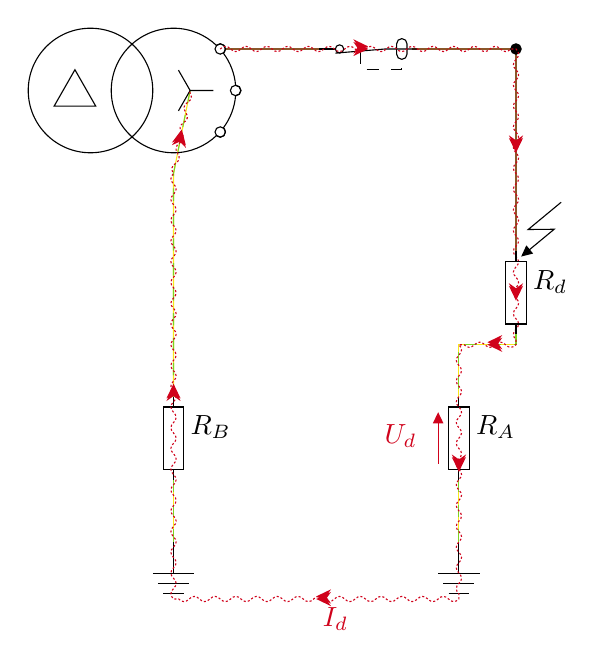
\begin{tikzpicture}[x=0.75pt,y=0.75pt,yscale=-1,xscale=1]
%uncomment if require: \path (0,353); %set diagram left start at 0, and has height of 353

%Straight Lines [id:da8450582290113836] 
\draw [color={rgb, 255:red, 248; green, 231; blue, 28 }  ,draw opacity=1 ]   (87.5,222.5) -- (87.5,252.5) ;
%Straight Lines [id:da035234150750507176] 
\draw [color={rgb, 255:red, 248; green, 231; blue, 28 }  ,draw opacity=1 ]   (252.5,152.5) -- (252.5,157.5) -- (225,157.5) -- (225,182.5) ;
%Straight Lines [id:da575921985906619] 
\draw [color={rgb, 255:red, 139; green, 87; blue, 42 }  ,draw opacity=1 ]   (112.5,15) -- (162.5,15) ;
%Straight Lines [id:da5726536295563455] 
\draw [color={rgb, 255:red, 248; green, 231; blue, 28 }  ,draw opacity=1 ]   (95.5,35) -- (87.5,75) -- (87.5,182.5) ;
%Straight Lines [id:da38476257001275427] 
\draw [color={rgb, 255:red, 126; green, 211; blue, 33 }  ,draw opacity=1 ] [dash pattern={on 4.5pt off 4.5pt}]  (95.5,35) -- (87.5,75) -- (87.5,182.5) ;
%Straight Lines [id:da9973940303994429] 
\draw [color={rgb, 255:red, 139; green, 87; blue, 42 }  ,draw opacity=1 ]   (202.5,15) -- (252.5,15) ;
%Shape: Path Data [id:dp9822778342813306] 
\draw   (112.5,55) .. controls (112.5,56.38) and (111.38,57.5) .. (110,57.5) .. controls (109.29,57.5) and (108.65,57.2) .. (108.19,56.72) .. controls (102.81,61.85) and (95.52,65) .. (87.5,65) .. controls (70.93,65) and (57.5,51.57) .. (57.5,35) .. controls (57.5,18.43) and (70.93,5) .. (87.5,5) .. controls (95.52,5) and (102.81,8.15) .. (108.19,13.28) .. controls (108.65,12.8) and (109.29,12.5) .. (110,12.5) .. controls (111.38,12.5) and (112.5,13.62) .. (112.5,15) .. controls (112.5,15.82) and (112.11,16.54) .. (111.5,17) .. controls (114.8,21.39) and (116.92,26.71) .. (117.4,32.5) .. controls (117.43,32.5) and (117.47,32.5) .. (117.5,32.5) .. controls (118.88,32.5) and (120,33.62) .. (120,35) .. controls (120,36.38) and (118.88,37.5) .. (117.5,37.5) .. controls (117.47,37.5) and (117.43,37.5) .. (117.4,37.5) .. controls (116.92,43.29) and (114.8,48.61) .. (111.5,53) .. controls (112.11,53.46) and (112.5,54.18) .. (112.5,55) -- cycle ;
%Shape: Circle [id:dp10169246549820965] 
\draw   (17.5,35) .. controls (17.5,18.43) and (30.93,5) .. (47.5,5) .. controls (64.07,5) and (77.5,18.43) .. (77.5,35) .. controls (77.5,51.57) and (64.07,65) .. (47.5,65) .. controls (30.93,65) and (17.5,51.57) .. (17.5,35) -- cycle ;
%Shape: Triangle [id:dp22185224755779764] 
\draw   (40,25) -- (30,42.5) -- (50,42.5) -- cycle ;
%Shape: Star [id:dp4535075510124722] 
\draw   (106.75,35) -- (95.5,35) -- (89.88,44.81) -- (95.5,35) -- (89.88,25.19) -- (95.5,35) -- cycle ;
%Shape: Circle [id:dp28187455970704567] 
\draw   (107.5,15) .. controls (107.5,13.62) and (108.62,12.5) .. (110,12.5) .. controls (111.38,12.5) and (112.5,13.62) .. (112.5,15) .. controls (112.5,16.38) and (111.38,17.5) .. (110,17.5) .. controls (108.62,17.5) and (107.5,16.38) .. (107.5,15) -- cycle ;
%Shape: Circle [id:dp9096244123377861] 
\draw   (114.9,35) .. controls (114.9,33.62) and (116.02,32.5) .. (117.4,32.5) .. controls (118.78,32.5) and (119.9,33.62) .. (119.9,35) .. controls (119.9,36.38) and (118.78,37.5) .. (117.4,37.5) .. controls (116.02,37.5) and (114.9,36.38) .. (114.9,35) -- cycle ;
%Shape: Circle [id:dp0660770114066822] 
\draw   (107.5,55) .. controls (107.5,53.62) and (108.62,52.5) .. (110,52.5) .. controls (111.38,52.5) and (112.5,53.62) .. (112.5,55) .. controls (112.5,56.38) and (111.38,57.5) .. (110,57.5) .. controls (108.62,57.5) and (107.5,56.38) .. (107.5,55) -- cycle ;

%Straight Lines [id:da12486709959480935] 
\draw [color={rgb, 255:red, 139; green, 87; blue, 42 }  ,draw opacity=1 ]   (252.5,112.5) -- (252.5,17.5) ;
%Straight Lines [id:da9194886303106931] 
\draw [color={rgb, 255:red, 126; green, 211; blue, 33 }  ,draw opacity=1 ] [dash pattern={on 4.5pt off 4.5pt}]  (252.5,152.5) -- (252.5,157.5) -- (225,157.5) -- (225,182.5) ;
%Straight Lines [id:da33889517147418446] 
\draw    (87.5,252.5) -- (87.5,267.5) ;
%Straight Lines [id:da7536356147270271] 
\draw    (77.5,267.5) -- (97.5,267.5) ;
%Straight Lines [id:da33790733335159795] 
\draw    (80,272.5) -- (95,272.5) ;
%Straight Lines [id:da8225336413065082] 
\draw    (82.5,277.5) -- (92.5,277.5) ;

%Straight Lines [id:da14728368722832463] 
\draw [color={rgb, 255:red, 126; green, 211; blue, 33 }  ,draw opacity=1 ] [dash pattern={on 4.5pt off 4.5pt}]  (87.5,222.5) -- (87.5,252.5) ;
%Straight Lines [id:da2713756434582886] 
\draw [color={rgb, 255:red, 248; green, 231; blue, 28 }  ,draw opacity=1 ]   (225,222.5) -- (225,252.5) ;
%Straight Lines [id:da07200185094723521] 
\draw    (225,252.5) -- (225,267.5) ;
%Straight Lines [id:da5503731135148442] 
\draw    (215,267.5) -- (235,267.5) ;
%Straight Lines [id:da9244125108161202] 
\draw    (217.5,272.5) -- (232.5,272.5) ;
%Straight Lines [id:da07512791048030887] 
\draw    (220,277.5) -- (230,277.5) ;

%Straight Lines [id:da5491926071123034] 
\draw [color={rgb, 255:red, 126; green, 211; blue, 33 }  ,draw opacity=1 ] [dash pattern={on 4.5pt off 4.5pt}]  (225,222.5) -- (225,252.5) ;
%Straight Lines [id:da7705666086878261] 
\draw    (87.5,217.5) -- (87.5,222.5) ;
%Shape: Rectangle [id:dp5724900932521552] 
\draw   (92.5,187.5) -- (92.5,217.5) -- (82.5,217.5) -- (82.5,187.5) -- cycle ;
%Straight Lines [id:da6857493814799358] 
\draw    (87.5,182.5) -- (87.5,187.5) ;

%Straight Lines [id:da7810225170823131] 
\draw    (225,217.5) -- (225,222.5) ;
%Shape: Rectangle [id:dp9839408028922504] 
\draw   (230,187.5) -- (230,217.5) -- (220,217.5) -- (220,187.5) -- cycle ;
%Straight Lines [id:da4367313473487816] 
\draw    (225,182.5) -- (225,187.5) ;

%Shape: Circle [id:dp6401617010113628] 
\draw  [fill={rgb, 255:red, 0; green, 0; blue, 0 }  ,fill opacity=1 ] (250,15) .. controls (250,13.62) and (251.12,12.5) .. (252.5,12.5) .. controls (253.88,12.5) and (255,13.62) .. (255,15) .. controls (255,16.38) and (253.88,17.5) .. (252.5,17.5) .. controls (251.12,17.5) and (250,16.38) .. (250,15) -- cycle ;
%Rounded Rect [id:dp9837999595449706] 
\draw   (197.5,20) .. controls (196.12,20) and (195,18.88) .. (195,17.5) -- (195,12.5) .. controls (195,11.12) and (196.12,10) .. (197.5,10) -- (197.5,10) .. controls (198.88,10) and (200,11.12) .. (200,12.5) -- (200,17.5) .. controls (200,18.88) and (198.88,20) .. (197.5,20) -- cycle ;
%Straight Lines [id:da04140906911364939] 
\draw  [dash pattern={on 4.5pt off 4.5pt}]  (177.5,16) -- (177.5,25) -- (197.5,25) -- (197.5,20) ;
%Shape: Circle [id:dp7012058816599942] 
\draw   (167.5,13) .. controls (166.4,13) and (165.5,13.9) .. (165.5,15) .. controls (165.5,16.1) and (166.4,17) .. (167.5,17) .. controls (168.6,17) and (169.5,16.1) .. (169.5,15) .. controls (169.5,13.9) and (168.6,13) .. (167.5,13) -- cycle ;
%Straight Lines [id:da23692932983683102] 
\draw    (165.5,15) -- (157.5,15) ;
%Straight Lines [id:da4567235518407359] 
\draw    (165.5,17) -- (189.5,15) -- (205,15) ;
%Shape: Boxed Line [id:dp44753967705251496] 
\draw    (274.27,88.83) -- (258.39,101.97) -- (270.89,101.86) -- (257.31,113.09) ;
\draw [shift={(255,115)}, rotate = 320.40999999999997] [fill={rgb, 255:red, 0; green, 0; blue, 0 }  ][line width=0.08]  [draw opacity=0] (5.36,-2.57) -- (0,0) -- (5.36,2.57) -- cycle    ;
\draw [color={rgb, 255:red, 208; green, 2; blue, 27 }  ,draw opacity=1 ] [dash pattern={on 0.75pt off 0.75pt}]  (110,15) .. controls (111.67,13.33) and (113.33,13.33) .. (115,15) .. controls (116.67,16.67) and (118.33,16.67) .. (120,15) .. controls (121.67,13.33) and (123.33,13.33) .. (125,15) .. controls (126.67,16.67) and (128.33,16.67) .. (130,15) .. controls (131.67,13.33) and (133.33,13.33) .. (135,15) .. controls (136.67,16.67) and (138.33,16.67) .. (140,15) .. controls (141.67,13.33) and (143.33,13.33) .. (145,15) .. controls (146.67,16.67) and (148.33,16.67) .. (150,15) .. controls (151.67,13.33) and (153.33,13.33) .. (155,15) .. controls (156.67,16.67) and (158.33,16.67) .. (160,15) .. controls (161.67,13.33) and (163.33,13.33) .. (165,15) .. controls (166.67,16.67) and (168.33,16.67) .. (170,15) .. controls (171.67,13.33) and (173.33,13.33) .. (175,15) .. controls (176.67,16.67) and (178.33,16.67) .. (180,15) .. controls (181.67,13.33) and (183.33,13.33) .. (185,15) .. controls (186.67,16.67) and (188.33,16.67) .. (190,15) .. controls (191.67,13.33) and (193.33,13.33) .. (195,15) .. controls (196.67,16.67) and (198.33,16.67) .. (200,15) .. controls (201.67,13.33) and (203.33,13.33) .. (205,15) .. controls (206.67,16.67) and (208.33,16.67) .. (210,15) .. controls (211.67,13.33) and (213.33,13.33) .. (215,15) .. controls (216.67,16.67) and (218.33,16.67) .. (220,15) .. controls (221.67,13.33) and (223.33,13.33) .. (225,15) .. controls (226.67,16.67) and (228.33,16.67) .. (230,15) .. controls (231.67,13.33) and (233.33,13.33) .. (235,15) .. controls (236.67,16.67) and (238.33,16.67) .. (240,15) .. controls (241.67,13.33) and (243.33,13.33) .. (245,15) .. controls (246.67,16.67) and (248.33,16.67) .. (250,15) -- (252.5,15) -- (252.5,15) .. controls (254.17,16.67) and (254.17,18.33) .. (252.5,20) .. controls (250.83,21.67) and (250.83,23.33) .. (252.5,25) .. controls (254.17,26.67) and (254.17,28.33) .. (252.5,30) .. controls (250.83,31.67) and (250.83,33.33) .. (252.5,35) .. controls (254.17,36.67) and (254.17,38.33) .. (252.5,40) .. controls (250.83,41.67) and (250.83,43.33) .. (252.5,45) .. controls (254.17,46.67) and (254.17,48.33) .. (252.5,50) .. controls (250.83,51.67) and (250.83,53.33) .. (252.5,55) .. controls (254.17,56.67) and (254.17,58.33) .. (252.5,60) .. controls (250.83,61.67) and (250.83,63.33) .. (252.5,65) .. controls (254.17,66.67) and (254.17,68.33) .. (252.5,70) .. controls (250.83,71.67) and (250.83,73.33) .. (252.5,75) .. controls (254.17,76.67) and (254.17,78.33) .. (252.5,80) .. controls (250.83,81.67) and (250.83,83.33) .. (252.5,85) .. controls (254.17,86.67) and (254.17,88.33) .. (252.5,90) .. controls (250.83,91.67) and (250.83,93.33) .. (252.5,95) .. controls (254.17,96.67) and (254.17,98.33) .. (252.5,100) .. controls (250.83,101.67) and (250.83,103.33) .. (252.5,105) .. controls (254.17,106.67) and (254.17,108.33) .. (252.5,110) .. controls (250.83,111.67) and (250.83,113.33) .. (252.5,115) -- (252.5,115) .. controls (254.17,116.67) and (254.17,118.33) .. (252.5,120) .. controls (250.83,121.67) and (250.83,123.33) .. (252.5,125) .. controls (254.17,126.67) and (254.17,128.33) .. (252.5,130) .. controls (250.83,131.67) and (250.83,133.33) .. (252.5,135) .. controls (254.17,136.67) and (254.17,138.33) .. (252.5,140) .. controls (250.83,141.67) and (250.83,143.33) .. (252.5,145) .. controls (254.17,146.67) and (254.17,148.33) .. (252.5,150) .. controls (250.83,151.67) and (250.83,153.33) .. (252.5,155) -- (252.5,157.5) -- (252.5,157.5) .. controls (250.83,159.17) and (249.17,159.17) .. (247.5,157.5) .. controls (245.83,155.83) and (244.17,155.83) .. (242.5,157.5) .. controls (240.83,159.17) and (239.17,159.17) .. (237.5,157.5) .. controls (235.83,155.83) and (234.17,155.83) .. (232.5,157.5) .. controls (230.83,159.17) and (229.17,159.17) .. (227.5,157.5) -- (225,157.5) -- (225,157.5) .. controls (226.67,159.17) and (226.67,160.83) .. (225,162.5) .. controls (223.33,164.17) and (223.33,165.83) .. (225,167.5) .. controls (226.67,169.17) and (226.67,170.83) .. (225,172.5) .. controls (223.33,174.17) and (223.33,175.83) .. (225,177.5) .. controls (226.67,179.17) and (226.67,180.83) .. (225,182.5) .. controls (223.33,184.17) and (223.33,185.83) .. (225,187.5) .. controls (226.67,189.17) and (226.67,190.83) .. (225,192.5) .. controls (223.33,194.17) and (223.33,195.83) .. (225,197.5) .. controls (226.67,199.17) and (226.67,200.83) .. (225,202.5) .. controls (223.33,204.17) and (223.33,205.83) .. (225,207.5) .. controls (226.67,209.17) and (226.67,210.83) .. (225,212.5) .. controls (223.33,214.17) and (223.33,215.83) .. (225,217.5) .. controls (226.67,219.17) and (226.67,220.83) .. (225,222.5) .. controls (223.33,224.17) and (223.33,225.83) .. (225,227.5) .. controls (226.67,229.17) and (226.67,230.83) .. (225,232.5) .. controls (223.33,234.17) and (223.33,235.83) .. (225,237.5) .. controls (226.67,239.17) and (226.67,240.83) .. (225,242.5) .. controls (223.33,244.17) and (223.33,245.83) .. (225,247.5) .. controls (226.67,249.17) and (226.67,250.83) .. (225,252.5) .. controls (223.33,254.17) and (223.33,255.83) .. (225,257.5) .. controls (226.67,259.17) and (226.67,260.83) .. (225,262.5) .. controls (223.33,264.17) and (223.33,265.83) .. (225,267.5) .. controls (226.67,269.17) and (226.67,270.83) .. (225,272.5) .. controls (223.33,274.17) and (223.33,275.83) .. (225,277.5) -- (225,280) -- (225,280) .. controls (223.33,281.67) and (221.67,281.67) .. (220,280) .. controls (218.33,278.33) and (216.67,278.33) .. (215,280) .. controls (213.33,281.67) and (211.67,281.67) .. (210,280) .. controls (208.33,278.33) and (206.67,278.33) .. (205,280) .. controls (203.33,281.67) and (201.67,281.67) .. (200,280) .. controls (198.33,278.33) and (196.67,278.33) .. (195,280) .. controls (193.33,281.67) and (191.67,281.67) .. (190,280) .. controls (188.33,278.33) and (186.67,278.33) .. (185,280) .. controls (183.33,281.67) and (181.67,281.67) .. (180,280) .. controls (178.33,278.33) and (176.67,278.33) .. (175,280) .. controls (173.33,281.67) and (171.67,281.67) .. (170,280) .. controls (168.33,278.33) and (166.67,278.33) .. (165,280) .. controls (163.33,281.67) and (161.67,281.67) .. (160,280) .. controls (158.33,278.33) and (156.67,278.33) .. (155,280) .. controls (153.33,281.67) and (151.67,281.67) .. (150,280) .. controls (148.33,278.33) and (146.67,278.33) .. (145,280) .. controls (143.33,281.67) and (141.67,281.67) .. (140,280) .. controls (138.33,278.33) and (136.67,278.33) .. (135,280) .. controls (133.33,281.67) and (131.67,281.67) .. (130,280) .. controls (128.33,278.33) and (126.67,278.33) .. (125,280) .. controls (123.33,281.67) and (121.67,281.67) .. (120,280) .. controls (118.33,278.33) and (116.67,278.33) .. (115,280) .. controls (113.33,281.67) and (111.67,281.67) .. (110,280) .. controls (108.33,278.33) and (106.67,278.33) .. (105,280) .. controls (103.33,281.67) and (101.67,281.67) .. (100,280) .. controls (98.33,278.33) and (96.67,278.33) .. (95,280) .. controls (93.33,281.67) and (91.67,281.67) .. (90,280) -- (87.5,280) -- (87.5,280) .. controls (85.83,278.33) and (85.83,276.67) .. (87.5,275) .. controls (89.17,273.33) and (89.17,271.67) .. (87.5,270) .. controls (85.83,268.33) and (85.83,266.67) .. (87.5,265) .. controls (89.17,263.33) and (89.17,261.67) .. (87.5,260) .. controls (85.83,258.33) and (85.83,256.67) .. (87.5,255) .. controls (89.17,253.33) and (89.17,251.67) .. (87.5,250) .. controls (85.83,248.33) and (85.83,246.67) .. (87.5,245) .. controls (89.17,243.33) and (89.17,241.67) .. (87.5,240) .. controls (85.83,238.33) and (85.83,236.67) .. (87.5,235) .. controls (89.17,233.33) and (89.17,231.67) .. (87.5,230) .. controls (85.83,228.33) and (85.83,226.67) .. (87.5,225) .. controls (89.17,223.33) and (89.17,221.67) .. (87.5,220) .. controls (85.83,218.33) and (85.83,216.67) .. (87.5,215) .. controls (89.17,213.33) and (89.17,211.67) .. (87.5,210) .. controls (85.83,208.33) and (85.83,206.67) .. (87.5,205) .. controls (89.17,203.33) and (89.17,201.67) .. (87.5,200) .. controls (85.83,198.33) and (85.83,196.67) .. (87.5,195) .. controls (89.17,193.33) and (89.17,191.67) .. (87.5,190) .. controls (85.83,188.33) and (85.83,186.67) .. (87.5,185) .. controls (89.17,183.33) and (89.17,181.67) .. (87.5,180) .. controls (85.83,178.33) and (85.83,176.67) .. (87.5,175) .. controls (89.17,173.33) and (89.17,171.67) .. (87.5,170) .. controls (85.83,168.33) and (85.83,166.67) .. (87.5,165) .. controls (89.17,163.33) and (89.17,161.67) .. (87.5,160) .. controls (85.83,158.33) and (85.83,156.67) .. (87.5,155) .. controls (89.17,153.33) and (89.17,151.67) .. (87.5,150) .. controls (85.83,148.33) and (85.83,146.67) .. (87.5,145) .. controls (89.17,143.33) and (89.17,141.67) .. (87.5,140) .. controls (85.83,138.33) and (85.83,136.67) .. (87.5,135) .. controls (89.17,133.33) and (89.17,131.67) .. (87.5,130) .. controls (85.83,128.33) and (85.83,126.67) .. (87.5,125) .. controls (89.17,123.33) and (89.17,121.67) .. (87.5,120) .. controls (85.83,118.33) and (85.83,116.67) .. (87.5,115) .. controls (89.17,113.33) and (89.17,111.67) .. (87.5,110) .. controls (85.83,108.33) and (85.83,106.67) .. (87.5,105) .. controls (89.17,103.33) and (89.17,101.67) .. (87.5,100) .. controls (85.83,98.33) and (85.83,96.67) .. (87.5,95) .. controls (89.17,93.33) and (89.17,91.67) .. (87.5,90) .. controls (85.83,88.33) and (85.83,86.67) .. (87.5,85) .. controls (89.17,83.33) and (89.17,81.67) .. (87.5,80) .. controls (85.83,78.33) and (85.83,76.67) .. (87.5,75) -- (87.5,75) .. controls (86.19,73.04) and (86.52,71.41) .. (88.48,70.1) .. controls (90.44,68.79) and (90.77,67.15) .. (89.46,65.19) .. controls (88.15,63.23) and (88.48,61.6) .. (90.44,60.29) .. controls (92.4,58.98) and (92.73,57.35) .. (91.42,55.39) .. controls (90.11,53.43) and (90.44,51.8) .. (92.4,50.49) .. controls (94.36,49.18) and (94.69,47.54) .. (93.38,45.58) .. controls (92.07,43.62) and (92.4,41.99) .. (94.36,40.68) .. controls (96.32,39.37) and (96.65,37.74) .. (95.34,35.78) -- (95.5,35) -- (95.5,35) ;
\draw [shift={(181.25,15)}, rotate = 180] [fill={rgb, 255:red, 208; green, 2; blue, 27 }  ,fill opacity=1 ][line width=0.08]  [draw opacity=0] (7.14,-3.43) -- (0,0) -- (7.14,3.43) -- (4.74,0) -- cycle    ;
\draw [shift={(252.5,65)}, rotate = 270] [fill={rgb, 255:red, 208; green, 2; blue, 27 }  ,fill opacity=1 ][line width=0.08]  [draw opacity=0] (7.14,-3.43) -- (0,0) -- (7.14,3.43) -- (4.74,0) -- cycle    ;
\draw [shift={(252.5,136.25)}, rotate = 270] [fill={rgb, 255:red, 208; green, 2; blue, 27 }  ,fill opacity=1 ][line width=0.08]  [draw opacity=0] (7.14,-3.43) -- (0,0) -- (7.14,3.43) -- (4.74,0) -- cycle    ;
\draw [shift={(238.75,157.5)}, rotate = 360] [fill={rgb, 255:red, 208; green, 2; blue, 27 }  ,fill opacity=1 ][line width=0.08]  [draw opacity=0] (7.14,-3.43) -- (0,0) -- (7.14,3.43) -- (4.74,0) -- cycle    ;
\draw [shift={(225,218.75)}, rotate = 270] [fill={rgb, 255:red, 208; green, 2; blue, 27 }  ,fill opacity=1 ][line width=0.08]  [draw opacity=0] (7.14,-3.43) -- (0,0) -- (7.14,3.43) -- (4.74,0) -- cycle    ;
\draw [shift={(156.25,280)}, rotate = 360] [fill={rgb, 255:red, 208; green, 2; blue, 27 }  ,fill opacity=1 ][line width=0.08]  [draw opacity=0] (7.14,-3.43) -- (0,0) -- (7.14,3.43) -- (4.74,0) -- cycle    ;
\draw [shift={(87.5,177.5)}, rotate = 450] [fill={rgb, 255:red, 208; green, 2; blue, 27 }  ,fill opacity=1 ][line width=0.08]  [draw opacity=0] (7.14,-3.43) -- (0,0) -- (7.14,3.43) -- (4.74,0) -- cycle    ;
\draw [shift={(91.5,55)}, rotate = 461.31] [fill={rgb, 255:red, 208; green, 2; blue, 27 }  ,fill opacity=1 ][line width=0.08]  [draw opacity=0] (7.14,-3.43) -- (0,0) -- (7.14,3.43) -- (4.74,0) -- cycle    ;
\draw [shift={(181.25,13.75)}, rotate = 180] [fill={rgb, 255:red, 208; green, 2; blue, 27 }  ,fill opacity=1 ][line width=0.08]  [draw opacity=0] (7.14,-3.43) -- (0,0) -- (7.14,3.43) -- (4.74,0) -- cycle    ;
\draw [shift={(252.5,63.75)}, rotate = 270] [fill={rgb, 255:red, 208; green, 2; blue, 27 }  ,fill opacity=1 ][line width=0.08]  [draw opacity=0] (7.14,-3.43) -- (0,0) -- (7.14,3.43) -- (4.74,0) -- cycle    ;
\draw [shift={(252.5,135)}, rotate = 270] [fill={rgb, 255:red, 208; green, 2; blue, 27 }  ,fill opacity=1 ][line width=0.08]  [draw opacity=0] (7.14,-3.43) -- (0,0) -- (7.14,3.43) -- (4.74,0) -- cycle    ;
\draw [shift={(238.75,156.25)}, rotate = 360] [fill={rgb, 255:red, 208; green, 2; blue, 27 }  ,fill opacity=1 ][line width=0.08]  [draw opacity=0] (7.14,-3.43) -- (0,0) -- (7.14,3.43) -- (4.74,0) -- cycle    ;
\draw [shift={(225,217.5)}, rotate = 270] [fill={rgb, 255:red, 208; green, 2; blue, 27 }  ,fill opacity=1 ][line width=0.08]  [draw opacity=0] (7.14,-3.43) -- (0,0) -- (7.14,3.43) -- (4.74,0) -- cycle    ;
\draw [shift={(156.25,278.75)}, rotate = 360] [fill={rgb, 255:red, 208; green, 2; blue, 27 }  ,fill opacity=1 ][line width=0.08]  [draw opacity=0] (7.14,-3.43) -- (0,0) -- (7.14,3.43) -- (4.74,0) -- cycle    ;
\draw [shift={(87.5,176.25)}, rotate = 450] [fill={rgb, 255:red, 208; green, 2; blue, 27 }  ,fill opacity=1 ][line width=0.08]  [draw opacity=0] (7.14,-3.43) -- (0,0) -- (7.14,3.43) -- (4.74,0) -- cycle    ;
\draw [shift={(91.5,53.75)}, rotate = 461.31] [fill={rgb, 255:red, 208; green, 2; blue, 27 }  ,fill opacity=1 ][line width=0.08]  [draw opacity=0] (7.14,-3.43) -- (0,0) -- (7.14,3.43) -- (4.74,0) -- cycle    ;
%Straight Lines [id:da9207949526828273] 
\draw    (252.5,147.5) -- (252.5,152.5) ;
%Shape: Rectangle [id:dp36210266951689685] 
\draw   (257.5,117.5) -- (257.5,147.5) -- (247.5,147.5) -- (247.5,117.5) -- cycle ;
%Straight Lines [id:da2843419817195654] 
\draw    (252.5,112.5) -- (252.5,117.5) ;

%Straight Lines [id:da667113945803525] 
\draw [color={rgb, 255:red, 208; green, 2; blue, 27 }  ,draw opacity=1 ]   (215,193) -- (215,215) ;
\draw [shift={(215,190)}, rotate = 90] [fill={rgb, 255:red, 208; green, 2; blue, 27 }  ,fill opacity=1 ][line width=0.08]  [draw opacity=0] (5.36,-2.57) -- (0,0) -- (5.36,2.57) -- cycle    ;

% Text Node
\draw (94.5,190.5) node [anchor=north west][inner sep=0.75pt]   [align=left] {$R_B$};
% Text Node
\draw (232,190.5) node [anchor=north west][inner sep=0.75pt]   [align=left] {$R_A$};
% Text Node
\draw (188,194.5) node [anchor=north west][inner sep=0.75pt]  [color={rgb, 255:red, 208; green, 2; blue, 27 }  ,opacity=1 ] [align=left] {$U_d$};
% Text Node
\draw (259.5,120.5) node [anchor=north west][inner sep=0.75pt]   [align=left] {$R_d$};
% Text Node
\draw (158.25,283) node [anchor=north west][inner sep=0.75pt] [color={rgb, 255:red, 208; green, 2; blue, 27 }]  [align=left] {$I_d$};


\end{tikzpicture}

\end{figure}

%\end{document}


\begin{comment}
\begin{circuitikz}[circuit ee IEC relay]
%\DrawGrid{(-1,-5)}{(9,3)} %grille d'aide pour le placement des objets

%alimentation

\node (D1) [make contact=point left, circuit breaker={point left}, tiny circuit symbols, activated] at (1,0.45) {};
\node (T1) [oosourcetransshape, prim=delta,sec=wye] at (0,0) {};


%neutre/terre

\node (RN) [R, label=$R_B$, rotate=90, tiny circuit symbols] at (0,-2.7) {};
\node (G1) [tlground] at (0,-3.9) {};
\draw [green!, thick] (G1) to node {} (RN) ; 
\draw [green!, thick] (RN) to (0,-0.5) to node {} (T1.sec4) ; 
\draw [dashed, yellow!, thick] (G1) to node {} (RN) ;
\draw [dashed, yellow!, thick] (RN) to (0,-0.5) to node {} (T1.sec4) ;

\node (RT) [resistor, rotate=90, tiny circuit symbols, label=$R_A$] at (2.5,-2.7) {};
\draw[-triangle 45, red] (2.8,-2) -- (2.8,-1) node[right,midway] {$U_d$};
\node (G2) [tlground] at (2.5,-3.9) {};
\draw [green!, thick] (RT) to (G2); 
\draw [dashed, yellow!, thick] (RT) to (G2);
\node (G2) [tlground] at (2.5,-3.9) {};
\draw [green!, thick] (G1) to (0,-4.2) to (2.5,-4.2) to (G2);
\draw [dashed, yellow!, thick] (G1) -- (0,-4.2) -- (2.5,-4.2) node [midway,below] {\color{black}$I_d$} -- (G2);
\node (G1) [tlground] at (0,-3.9) {};
\node (G2) [tlground] at (2.5,-3.9) {};

%appareil 1

\node (C2) [circ, scale=0.5] at (2.5,0.45) {};
\node (RD) [resistor, label=$R_d$, rotate=90, tiny circuit symbols] at (2.5,-1.5) {};

\draw [green!, thick] (RD) to (RT); 
\draw [dashed, yellow!, thick] (RD) to (RT); 

\draw [brown, thick] (T1.sec1) to (0.5,0.45) to (D1) to (C2) to (RD);
\node (T1) [oosourcetransshape, prim=delta,sec=wye] at (0,0) {};

%chemin courant

\fill [yellow!, decoration=lightning bolt, decorate] (2.5,-1.2) -- ++ (0.5,0.8); %éclairs
\path [postaction={on each segment={mid arrow=red}}]  (T1.sec1) -- (0.5,0.45) -- (D1) -- (C2) -- (RD) -- (RT) -- (G2) -- (2.5,-4.2) -- (1.666,-4.2) -- (0.88888,-4.2)  -- (0,-4.2) -- (G1) -- (RN) -- (0,-0.5) -- (T1.sec4); 

\callout{1,-0.5}{\cstep\label{pas:1}}{2.4,-1.2};


\end{circuitikz}
\end{comment}


L'intensité de courant $I_d$ vaut alors :
\begin{formule}[Courant de défaut $I_d$]
\begin{align}
		I_d &= \frac{V}{R_{B}+R_{A}+R_{d}}
\end{align}
\end{formule}

\begin{textvariables}
V								& tension							& volt			& \volt					& 	Différence de potentiel entre les masses métalliques et la terre 	\\
R_{B}						& résistance						& ohm			& \ohm					& 	Résistance de la prise de terre du neutre 	\\
R_{A}						& résistance						& ohm			& \ohm					& 	Résistance de la prise de terre de l'installation électrique 	\\
R_{d}						& résistance						& ohm			& \ohm					& 	Résistance de défaut 	d'isolement \\
\end{textvariables}

Le courant de défaut $I_d$ fera alors apparaître une \emph{tension de défaut} $U_d$ entre la masse métallique et la terre. Pour satisfaire aux normes de sécurité de la NF C15-100, il est imposé que la tension de défaut $U_d$ ne dépasse pas la tension de sécurité du local $U_L$ (voir \superref{subsec:prise_terre_installation_electrique}) :

\begin{formule}[Tension de défaut $U_d$]
\begin{align}
		U_d &= R_{A} \cdot I_{d} \\
			   &< U_L
\end{align}
\end{formule}

\begin{textvariables}
R_{A}						& résistance						& ohm			& \ohm					& 	Résistance de la prise de terre de l'installation électrique 	\\
I_{d}							& intensité							& ampère		& \ampere				& 	Courant de défaut d'isolement \\
U_{L}						& tension							& volt			& \volt					& 	Tension de sécurité du local avec :
\begin{description}[nosep, leftmargin=*]
\item[Local sec :] $U_{L}=\SI{50}{\volt}$
\item[Local humide :] $U_{L}=\SI{25}{\volt}$
\end{description} \\
\end{textvariables}

Il est donc nécessaire de limiter $U_d$ à la valeur suivante (voir \superref{form:resistance_prise_terre}) :

\begin{formule}[Calibre du DDR $I_{\Delta n}$]
\begin{align}
		I_{\Delta n} &< \frac{U_{L}}{R_{A}}
\end{align}
\end{formule}

\begin{textvariables}
U_{L}						& tension							& volt			& \volt					& 	Tension de sécurité du local avec :
\begin{description}[nosep, leftmargin=*]
\item[Local sec :] $U_{L}=\SI{50}{\volt}$
\item[Local humide :] $U_{L}=\SI{25}{\volt}$
\end{description} \\
R_{A}						& résistance						& ohm			& \ohm					& 	Résistance de la prise de terre de l'installation électrique 	\\
\end{textvariables}

\begin{exemple}[Calcul du calibre du DDR $I_{\Delta n}$]
Si on considère que le transformateur est un transformateur $\SI{20}{\kilo\volt}/\SI{400}{\volt}$, que $R_A=\SI{20}{\ohm}$, que $R_B=\SI{10}{\ohm}$ et que $R_d$ est négligée, on peut déduire que le courant de défaut $I_d$ vaut :
\begin{align*}
		I_d 	&= \frac{V}{R_{B}+R_{A}} \\
				&=\frac{400}{20+10} \\
				&= \SI{13,33}{\ampere} \\
\end{align*}
Si une personne touche une masse des récepteurs en défaut, elle sera soumise à une tension de défaut $U_d$ :
\begin{align*}
		U_d 	&= R_{A} \cdot I_{d} \\
				&=20 \cdot 13,33 \\
				&= \SI{266,6}{\volt}
\end{align*}
La tension de défaut $U_d$ est dangereuse quelle que soit la tension limite choisie :
\begin{itemize}
\item coupure la plus rapide possible\,;
\item protection des personnes.
\end{itemize}
~\\
\begin{minipage}[t]{0.5\linewidth}
Dans le cas d'un local sec :
\begin{align*}
	I_{\Delta n} 	&< \frac{U_{L}}{R_{A}} \\
						&< \frac{50}{20} \\
						&< \SI{2,5}{\ampere}
\end{align*}
\end{minipage}
\hfill
\begin{minipage}[t]{0.5\linewidth}
Dans le cas d'un local humide :
\begin{align*}
	I_{\Delta n} 	&< \frac{U_{L}}{R_{A}} \\
						&< \frac{25}{20} \\
						&< \SI{1,25}{\ampere}
\end{align*}
\end{minipage}
~\\
D'après le tableau situé en \superref{tab:temps_coupure_DDR}, le DDR doit présenter un temps de coupure de moins de \SI{70}{\milli\second} avec une tension de défaut $U_d$ de \SI{266,6}{\volt} :

\begin{table}[h]
\begin{tabularx}{\linewidth}{X cccccccc}
\toprule
Tension nominale		& \multicolumn{2}{c}{$\SI{50}{\volt}<U_0\leq\SI{120}{\volt}$} 	& \multicolumn{2}{c}{$\SI{120}{\volt}<U_0\leq\SI{230}{\volt}$} & \multicolumn{2}{c}{$\SI{230}{\volt}<U_0\leq\SI{400}{\volt}$}		& \multicolumn{2}{c}{$U_0>\SI{400}{\volt}$}\\
\midrule
Type de courant		& alternatif	& continu	& alternatif	& continu	& alternatif	& continu	& alternatif	& continu \\
\addlinespace
Schéma TN/IT	& \SI{0,8}{\second}	&	\SI{5}{\second}	&	\SI{0,4}{\second}	&	\SI{5}{\second}	&	\SI{0,2}{\second}	&	\SI{0,4}{\second}	&	\SI{0,1}{\second}	&	\SI{0,1}{\second} \\	
\addlinespace
Schéma TT	& \SI{0,3}{\second}	&	\SI{5}{\second}	&	\SI{0,2}{\second}	&	\SI{0,4}{\second}	&	\cellcolor{green}\SI{0,07}{\second}	&	\SI{0,2}{\second}	&	\SI{0,04}{\second}	&	\SI{0,1}{\second} \\	
\bottomrule
\end{tabularx}
\end{table}
\end{exemple}

%\end{document}

	%--------------------------------------
%ELECTROTECHNIQUE - SCHEMA DE LIAISON A LA TERRE
%--------------------------------------

%utiliser les environnement \begin{comment} \end{comment} pour mettre en commentaire le préambule une fois la programmation appelée dans le document maître (!ne pas oublier de mettre en commentaire \end{document}!)


\documentclass[a4paper, 11pt, twoside, fleqn]{memoir}

\usepackage{AOCDTF}
\typemedia{paper} %choix screen ou paper pour les vidéos et schémas animés

\marqueurchapitre
\decoupagechapitre{1} %juste pour éviter les erreurs lors de la compilation des sous-programmations (passera en commentaire)

%--------------------------------------
%corps du document
%--------------------------------------

\begin{document} %corps du document
	\openleft %début de chapitre à gauche


\chapter{Schéma Terre-Neutre\label{chap:schema_tn}}
\ChapFrame

\section{Caractéristiques générales}

\begin{definition}{Schéma TN}{}
Schéma de liaison à la terre dans lequel :
\begin{description}
\item[Neutre :] relié à la terre\,;
\item[Masses :] reliées au neutre du transformateur HT/BT.
\end{description}
\end{definition}

Dans le SLT TN, le point neutre du transformateur HT/BT (point commun) est relié à la terre via la \emph{prise de terre du neutre}. Cette liaison présente une certaine résistance, la \emph{résistance de la prise de terre du neutre} $R_B$. Sa mise en \oe{}uvre est à charge du fournisseur d'électricité et sa résistance globale doit être inférieure ou égale à \SI{15}{\ohm} \supercite{NF:C13-100-2015}.\\

Les masses sont quant à elles reliées au point neutre du transformateur HT/BT (point commun), cela peut être réalisé via trois déclinaisons du SLT TN :

%--------------------------------------
%ELECTROTECHNIQUE - SCHEMA DE LIAISON A LA TERRE
%--------------------------------------

%utiliser les environnement \begin{comment} \end{comment} pour mettre en commentaire le préambule une fois la programmation appelée dans le document maître (!ne pas oublier de mettre en commentaire \end{document}!)

\begin{comment}

\documentclass[a4paper, 11pt, twoside, fleqn]{memoir}

\usepackage{AOCDTF}

\marqueurchapitre

%lien d'édition des figures Tikz sur le site mathcha.io (rajouter le lien d'une modification effectuée sur la figure tikz avec le nom du modificateur car il n'y a qu'un lien par compte)

%lien mathcha Nom Prénom : 

%--------------------------------------
%corps du document
%--------------------------------------

\begin{document} %corps du document
	\openleft %début de chapitre à gauche

\end{comment}

\begin{xltabular}{\textwidth}{C >{\compress}X >{\compress}X >{\compress}X}
\caption{Déclinaisons du SLT TN}\\
\toprule
\thead{Nom}		& \thead{Caractéristiques}		& \thead{Avantages}		& \thead{Inconvénients} \\
\midrule
\endfirsthead %en-tête de la première page du tableau  
\multicolumn{4}{l}{\small\textit{Page précédente}} \\
\midrule %filet de milieu de tableau
\thead{Nom}		& \thead{Caractéristique}		& \thead{Avantages} 	& \thead{Inconvénients} \\
\midrule
\endhead
\midrule %filet de milieu de tableau
\multicolumn{4}{r}{\small\textit{Page suivante}} \\
\endfoot %pied de page de toutes les pages du tableau
\bottomrule
\endlastfoot %pied de page de la dernièredu tableau
Confondus (TN-C)		
& 
\begin{tabitemize}
\item conducteurs neutre et PE confondus\,;
\item PE et neutre vert/jaune nommé conducteur Protection \'Equipotentielle Neutre (PEN).
\end{tabitemize}
&
\begin{tabitemize}
\item économie d'un câble.
\end{tabitemize}
&		
\begin{tabitemize}
\item utilisation de canalisations fixes et rigides.
\item interdiction de pose :
	\begin{compactitemize}
	\item locaux à risques d'incendies\,;
	\item alimentation d'équipements de traitement de l'information (présence de courant harmonique dans le neutre).
	\end{compactitemize}
\end{tabitemize}\\
\addlinespace
Séparés (TN-S)		
&
\begin{tabitemize}
\item conducteurs neutre et PE séparés\,;
\item PE et neutre vert/jaune séparés (PE+N).
\end{tabitemize}
&
\begin{tabitemize}
\item usage de conducteurs souples autorisés\,;
\item séparation et protection du neutre possibles dans les locaux pollués.
\end{tabitemize}
&
\begin{tabitemize}
\item solution plus coûteuse que le schéma TN-C.
\end{tabitemize}
\\
\addlinespace
Mixte (TN-C-S)	
&
\begin{tabitemize}
\item combinaison des SLT TN-C et TN-S dans une même installation\,;
\item usage du SLT TN-C formellement interdit en aval du SLT TN-S.
\end{tabitemize}
&
\begin{tabitemize}
\item combinaison des avantages des deux SLT TN.
\end{tabitemize}
&\\
\end{xltabular}


%\end{document}



Ce SLT présente les caractéristiques principales suivantes :
\begin{itemize}
\item utilisation uniquement dans les installations électriques alimentées par un transformateur HT/BT (ou MT/BT ou BT/BT)\,;
\item requiert l'installation de prises de terre uniformément réparties dans l'installation\,;
\item requiert la vérification des déclenchements sur le premier défaut d'isolement, obtenue lors de l'étude par des calculs de dimensionnement et, lors de la mise en service par des mesures de test\,; 
\item ne requiert pas de DDR dans l'absolu\,;
\item requiert un installateur qualifié pour toute installation, modification ou encore extension\,;
\item pouvant endommager de manière plus significative les bobinages et appareillages lors d'un défaut d'isolement, par rapport au SLT TT\,;
\item danger plus élevé dans les locaux à risque d'incendie du fait de courants de défaut plus importants.
\end{itemize}

\section{Schémas de principe}

\begin{figure}[H]
\caption{Installation Terre-Neutre Confondus}
\begin{subfigure}[t]{0.49\linewidth}
%--------------------------------------
%ELECTROTECHNIQUE - SCHEMA DE LIAISON A LA TERRE
%--------------------------------------

%utiliser les environnement \begin{comment} \end{comment} pour mettre en commentaire le préambule une fois la programmation appelée dans le document maître (!ne pas oublier de mettre en commentaire \end{document}!)

\begin{comment}

\documentclass{standalone}

\usepackage{physics}
\usepackage{amsmath}
\usepackage{tikz}
\usepackage{mathdots}
\usepackage{yhmath}
\usepackage{cancel}
\usepackage{color}
\usepackage{siunitx}
\usepackage{array}
\usepackage{multirow}
\usepackage{amssymb}
\usepackage{gensymb}
\usepackage{tabularx}
\usepackage{booktabs}
\usetikzlibrary{fadings}
\usetikzlibrary{patterns}
\usetikzlibrary{shadows.blur}
\usetikzlibrary{shapes}

%lien d'édition des figures Tikz sur le site mathcha.io (rajouter le lien d'une modification effectuée sur la figure tikz avec le nom du modificateur car il n'y a qu'un lien par compte)

%lien mathcha Bruno Douchy : https://www.mathcha.io/editor/BkoJxFBDtnquyDl58vhj68k04ikMPoQOHQ2gjOW

%--------------------------------------
%corps du document
%--------------------------------------

\begin{document} %corps du document

\end{comment}




% Pattern Info
 
\tikzset{
pattern size/.store in=\mcSize, 
pattern size = 5pt,
pattern thickness/.store in=\mcThickness, 
pattern thickness = 0.3pt,
pattern radius/.store in=\mcRadius, 
pattern radius = 1pt}
\makeatletter
\pgfutil@ifundefined{pgf@pattern@name@_v1tzu2pxh}{
\pgfdeclarepatternformonly[\mcThickness,\mcSize]{_v1tzu2pxh}
{\pgfqpoint{0pt}{0pt}}
{\pgfpoint{\mcSize+\mcThickness}{\mcSize+\mcThickness}}
{\pgfpoint{\mcSize}{\mcSize}}
{
\pgfsetcolor{\tikz@pattern@color}
\pgfsetlinewidth{\mcThickness}
\pgfpathmoveto{\pgfqpoint{0pt}{0pt}}
\pgfpathlineto{\pgfpoint{\mcSize+\mcThickness}{\mcSize+\mcThickness}}
\pgfusepath{stroke}
}}
\makeatother
\tikzset{every picture/.style={line width=0.5pt}} %set default line width to 0.75pt        

\begin{tikzpicture}[x=0.75pt,y=0.75pt,yscale=-0.6,xscale=0.6]
%uncomment if require: \path (0,251); %set diagram left start at 0, and has height of 251

%Straight Lines [id:da008483698413953467] 
\draw [color={rgb, 255:red, 248; green, 231; blue, 28 }  ,draw opacity=1 ]   (90,75) -- (460,75) ;
%Straight Lines [id:da06944587101382871] 
\draw [color={rgb, 255:red, 126; green, 211; blue, 33 }  ,draw opacity=1 ] [dash pattern={on 2.25pt off 2.25pt}]  (90,75) -- (460,75) ;
%Straight Lines [id:da7402424217268804] 
\draw [color={rgb, 255:red, 248; green, 231; blue, 28 }  ,draw opacity=1 ]   (87.5,162.5) -- (87.5,192.5) ;
%Straight Lines [id:da5918343393245601] 
\draw [color={rgb, 255:red, 248; green, 231; blue, 28 }  ,draw opacity=1 ]   (240,135) -- (225,135) -- (225,75) ;
%Straight Lines [id:da8855218059773354] 
\draw    (120,35) -- (162.5,35) ;
%Straight Lines [id:da4387311249705095] 
\draw [color={rgb, 255:red, 139; green, 87; blue, 42 }  ,draw opacity=1 ]   (112.5,15) -- (162.5,15) ;
%Straight Lines [id:da636953775291555] 
\draw [color={rgb, 255:red, 155; green, 155; blue, 155 }  ,draw opacity=1 ]   (112.5,55) -- (162.5,55) ;
%Straight Lines [id:da6725148311968068] 
\draw [color={rgb, 255:red, 248; green, 231; blue, 28 }  ,draw opacity=1 ]   (95.5,35) -- (87.5,75) -- (87.5,122.5) ;
%Straight Lines [id:da09238729671521517] 
\draw [color={rgb, 255:red, 126; green, 211; blue, 33 }  ,draw opacity=1 ] [dash pattern={on 2.25pt off 2.25pt}]  (95.5,35) -- (87.5,75) -- (87.5,122.5) ;
%Straight Lines [id:da8100957998136087] 
\draw    (202.5,35) -- (460,35) ;
%Straight Lines [id:da16093045358944136] 
\draw [color={rgb, 255:red, 139; green, 87; blue, 42 }  ,draw opacity=1 ]   (202.5,15) -- (460,15) ;
%Straight Lines [id:da20849694685551212] 
\draw [color={rgb, 255:red, 155; green, 155; blue, 155 }  ,draw opacity=1 ]   (202.5,55) -- (460,55) ;
%Shape: Path Data [id:dp6834291829337227] 
\draw   (112.5,55) .. controls (112.5,56.38) and (111.38,57.5) .. (110,57.5) .. controls (109.29,57.5) and (108.65,57.2) .. (108.19,56.72) .. controls (102.81,61.85) and (95.52,65) .. (87.5,65) .. controls (70.93,65) and (57.5,51.57) .. (57.5,35) .. controls (57.5,18.43) and (70.93,5) .. (87.5,5) .. controls (95.52,5) and (102.81,8.15) .. (108.19,13.28) .. controls (108.65,12.8) and (109.29,12.5) .. (110,12.5) .. controls (111.38,12.5) and (112.5,13.62) .. (112.5,15) .. controls (112.5,15.82) and (112.11,16.54) .. (111.5,17) .. controls (114.8,21.39) and (116.92,26.71) .. (117.4,32.5) .. controls (117.43,32.5) and (117.47,32.5) .. (117.5,32.5) .. controls (118.88,32.5) and (120,33.62) .. (120,35) .. controls (120,36.38) and (118.88,37.5) .. (117.5,37.5) .. controls (117.47,37.5) and (117.43,37.5) .. (117.4,37.5) .. controls (116.92,43.29) and (114.8,48.61) .. (111.5,53) .. controls (112.11,53.46) and (112.5,54.18) .. (112.5,55) -- cycle ;
%Shape: Circle [id:dp25520013984238377] 
\draw   (17.5,35) .. controls (17.5,18.43) and (30.93,5) .. (47.5,5) .. controls (64.07,5) and (77.5,18.43) .. (77.5,35) .. controls (77.5,51.57) and (64.07,65) .. (47.5,65) .. controls (30.93,65) and (17.5,51.57) .. (17.5,35) -- cycle ;
%Shape: Triangle [id:dp16879536749213853] 
\draw   (40,25) -- (30,42.5) -- (50,42.5) -- cycle ;
%Shape: Star [id:dp24745133775448547] 
\draw   (106.75,35) -- (95.5,35) -- (89.88,44.81) -- (95.5,35) -- (89.88,25.19) -- (95.5,35) -- cycle ;
%Shape: Circle [id:dp9864849188587985] 
\draw   (107.5,15) .. controls (107.5,13.62) and (108.62,12.5) .. (110,12.5) .. controls (111.38,12.5) and (112.5,13.62) .. (112.5,15) .. controls (112.5,16.38) and (111.38,17.5) .. (110,17.5) .. controls (108.62,17.5) and (107.5,16.38) .. (107.5,15) -- cycle ;
%Shape: Circle [id:dp03445318892672977] 
\draw   (114.9,35) .. controls (114.9,33.62) and (116.02,32.5) .. (117.4,32.5) .. controls (118.78,32.5) and (119.9,33.62) .. (119.9,35) .. controls (119.9,36.38) and (118.78,37.5) .. (117.4,37.5) .. controls (116.02,37.5) and (114.9,36.38) .. (114.9,35) -- cycle ;
%Shape: Circle [id:dp21435391141876436] 
\draw   (107.5,55) .. controls (107.5,53.62) and (108.62,52.5) .. (110,52.5) .. controls (111.38,52.5) and (112.5,53.62) .. (112.5,55) .. controls (112.5,56.38) and (111.38,57.5) .. (110,57.5) .. controls (108.62,57.5) and (107.5,56.38) .. (107.5,55) -- cycle ;

%Straight Lines [id:da9414980338893979] 
\draw [color={rgb, 255:red, 74; green, 144; blue, 226 }  ,draw opacity=1 ]   (292.5,112.5) -- (292.5,77.5) ;
%Straight Lines [id:da27751530095615806] 
\draw [color={rgb, 255:red, 139; green, 87; blue, 42 }  ,draw opacity=1 ]   (252.5,112.5) -- (252.5,17.5) ;
%Straight Lines [id:da8401783030061442] 
\draw [color={rgb, 255:red, 139; green, 87; blue, 42 }  ,draw opacity=1 ]   (252.5,130) -- (252.5,117.5) ;
%Straight Lines [id:da6144198142388259] 
\draw [color={rgb, 255:red, 74; green, 144; blue, 226 }  ,draw opacity=1 ]   (292.5,130.5) -- (292.5,117.5) ;
%Straight Lines [id:da08447178364240893] 
\draw    (45,172.5) -- (460,172.5) ;
%Shape: Rectangle [id:dp6917865548447948] 
\draw  [draw opacity=0][pattern=_v1tzu2pxh,pattern size=6pt,pattern thickness=0.75pt,pattern radius=0pt, pattern color={rgb, 255:red, 0; green, 0; blue, 0}][line width=0.75]  (45,172.5) -- (460,172.5) -- (460,187.5) -- (45,187.5) -- cycle ;
%Straight Lines [id:da5758120659627904] 
\draw [color={rgb, 255:red, 126; green, 211; blue, 33 }  ,draw opacity=1 ] [dash pattern={on 2.25pt off 2.25pt}]  (240,135) -- (225,135) -- (225,75) ;
%Straight Lines [id:da3042650335499705] 
\draw    (87.5,192.5) -- (87.5,207.5) ;
%Straight Lines [id:da5819552828178339] 
\draw    (77.5,207.5) -- (97.5,207.5) ;
%Straight Lines [id:da5191842943668726] 
\draw    (80,212.5) -- (95,212.5) ;
%Straight Lines [id:da20267125061533042] 
\draw    (82.5,217.5) -- (92.5,217.5) ;

%Straight Lines [id:da1731291153518706] 
\draw [color={rgb, 255:red, 126; green, 211; blue, 33 }  ,draw opacity=1 ] [dash pattern={on 2.25pt off 2.25pt}]  (87.5,162.5) -- (87.5,192.5) ;
%Straight Lines [id:da447845422109466] 
\draw    (287.5,130) -- (292.5,130) ;
%Shape: Rectangle [id:dp520581263360185] 
\draw   (257.5,125) -- (287.5,125) -- (287.5,135) -- (257.5,135) -- cycle ;
%Straight Lines [id:da5356387601329091] 
\draw    (252.5,130) -- (257.5,130) ;

%Straight Lines [id:da07643260567103483] 
\draw    (87.5,157.5) -- (87.5,162.5) ;
%Shape: Rectangle [id:dp008342316051101917] 
\draw   (92.5,127.5) -- (92.5,157.5) -- (82.5,157.5) -- (82.5,127.5) -- cycle ;
%Straight Lines [id:da09697746232408333] 
\draw    (87.5,122.5) -- (87.5,127.5) ;

%Straight Lines [id:da1742958722449034] 
\draw [color={rgb, 255:red, 248; green, 231; blue, 28 }  ,draw opacity=1 ]   (325,135) -- (310,135) -- (310,75) ;
%Straight Lines [id:da016656189472749827] 
\draw [color={rgb, 255:red, 74; green, 144; blue, 226 }  ,draw opacity=1 ]   (377.5,112.5) -- (377.5,77.5) ;
%Straight Lines [id:da09528364052879534] 
\draw [color={rgb, 255:red, 139; green, 87; blue, 42 }  ,draw opacity=1 ]   (337.5,112.5) -- (337.5,17.5) ;
%Straight Lines [id:da31579551999326805] 
\draw [color={rgb, 255:red, 139; green, 87; blue, 42 }  ,draw opacity=1 ]   (337.5,130) -- (337.5,117.5) ;
%Straight Lines [id:da8299851447706146] 
\draw [color={rgb, 255:red, 74; green, 144; blue, 226 }  ,draw opacity=1 ]   (377.5,130.5) -- (377.5,117.5) ;
%Straight Lines [id:da33732409899195637] 
\draw [color={rgb, 255:red, 126; green, 211; blue, 33 }  ,draw opacity=1 ] [dash pattern={on 2.25pt off 2.25pt}]  (325,135) -- (310,135) -- (310,75) ;
%Straight Lines [id:da44333407130344615] 
\draw    (372.5,130) -- (377.5,130) ;
%Shape: Rectangle [id:dp8912988160440456] 
\draw   (342.5,125) -- (372.5,125) -- (372.5,135) -- (342.5,135) -- cycle ;
%Straight Lines [id:da6881533641386929] 
\draw    (337.5,130) -- (342.5,130) ;

%Straight Lines [id:da9265870438738062] 
\draw [color={rgb, 255:red, 248; green, 231; blue, 28 }  ,draw opacity=1 ]   (410,135) -- (395,135) -- (395,75) ;
%Straight Lines [id:da29888425275861696] 
\draw [color={rgb, 255:red, 74; green, 144; blue, 226 }  ,draw opacity=1 ]   (462.5,112.5) -- (462.5,77.5) ;
%Straight Lines [id:da19160803833752127] 
\draw [color={rgb, 255:red, 139; green, 87; blue, 42 }  ,draw opacity=1 ]   (422.5,112.5) -- (422.5,17.5) ;
%Straight Lines [id:da2386502061815522] 
\draw [color={rgb, 255:red, 139; green, 87; blue, 42 }  ,draw opacity=1 ]   (422.5,130) -- (422.5,117.5) ;
%Straight Lines [id:da8099974104215516] 
\draw [color={rgb, 255:red, 74; green, 144; blue, 226 }  ,draw opacity=1 ]   (462.5,130.5) -- (462.5,117.5) ;
%Straight Lines [id:da5974904676194153] 
\draw [color={rgb, 255:red, 126; green, 211; blue, 33 }  ,draw opacity=1 ] [dash pattern={on 2.25pt off 2.25pt}]  (410,135) -- (395,135) -- (395,75) ;
%Straight Lines [id:da24571432228663814] 
\draw    (457.5,130) -- (462.5,130) ;
%Shape: Rectangle [id:dp7341042129075479] 
\draw   (427.5,125) -- (457.5,125) -- (457.5,135) -- (427.5,135) -- cycle ;
%Straight Lines [id:da8263877672394346] 
\draw    (422.5,130) -- (427.5,130) ;

%Shape: Circle [id:dp7480136730647264] 
\draw  [fill={rgb, 255:red, 0; green, 0; blue, 0 }  ,fill opacity=1 ] (375,75) .. controls (375,73.62) and (376.12,72.5) .. (377.5,72.5) .. controls (378.88,72.5) and (380,73.62) .. (380,75) .. controls (380,76.38) and (378.88,77.5) .. (377.5,77.5) .. controls (376.12,77.5) and (375,76.38) .. (375,75) -- cycle ;
%Shape: Circle [id:dp20106995777905023] 
\draw  [fill={rgb, 255:red, 0; green, 0; blue, 0 }  ,fill opacity=1 ] (460,75) .. controls (460,73.62) and (461.12,72.5) .. (462.5,72.5) .. controls (463.88,72.5) and (465,73.62) .. (465,75) .. controls (465,76.38) and (463.88,77.5) .. (462.5,77.5) .. controls (461.12,77.5) and (460,76.38) .. (460,75) -- cycle ;
%Shape: Circle [id:dp30375287231255577] 
\draw  [fill={rgb, 255:red, 0; green, 0; blue, 0 }  ,fill opacity=1 ] (335,15) .. controls (335,13.62) and (336.12,12.5) .. (337.5,12.5) .. controls (338.88,12.5) and (340,13.62) .. (340,15) .. controls (340,16.38) and (338.88,17.5) .. (337.5,17.5) .. controls (336.12,17.5) and (335,16.38) .. (335,15) -- cycle ;
%Shape: Circle [id:dp1979307718008253] 
\draw  [fill={rgb, 255:red, 0; green, 0; blue, 0 }  ,fill opacity=1 ] (420,15) .. controls (420,13.62) and (421.12,12.5) .. (422.5,12.5) .. controls (423.88,12.5) and (425,13.62) .. (425,15) .. controls (425,16.38) and (423.88,17.5) .. (422.5,17.5) .. controls (421.12,17.5) and (420,16.38) .. (420,15) -- cycle ;
%Shape: Circle [id:dp08277262683691078] 
\draw  [fill={rgb, 255:red, 0; green, 0; blue, 0 }  ,fill opacity=1 ] (290,75) .. controls (290,73.62) and (291.12,72.5) .. (292.5,72.5) .. controls (293.88,72.5) and (295,73.62) .. (295,75) .. controls (295,76.38) and (293.88,77.5) .. (292.5,77.5) .. controls (291.12,77.5) and (290,76.38) .. (290,75) -- cycle ;
%Shape: Circle [id:dp2507630610609335] 
\draw  [fill={rgb, 255:red, 0; green, 0; blue, 0 }  ,fill opacity=1 ] (250,15) .. controls (250,13.62) and (251.12,12.5) .. (252.5,12.5) .. controls (253.88,12.5) and (255,13.62) .. (255,15) .. controls (255,16.38) and (253.88,17.5) .. (252.5,17.5) .. controls (251.12,17.5) and (250,16.38) .. (250,15) -- cycle ;
%Shape: Rectangle [id:dp19008190111612866] 
\draw  [dash pattern={on 2.25pt off 2.25pt on 1pt off 2.25pt}] (242.5,115) -- (302.5,115) -- (302.5,145) -- (242.5,145) -- cycle ;
%Shape: Circle [id:dp22840916642995968] 
\draw  [fill={rgb, 255:red, 255; green, 255; blue, 255 }  ,fill opacity=1 ] (240,135) .. controls (240,133.62) and (241.12,132.5) .. (242.5,132.5) .. controls (243.88,132.5) and (245,133.62) .. (245,135) .. controls (245,136.38) and (243.88,137.5) .. (242.5,137.5) .. controls (241.12,137.5) and (240,136.38) .. (240,135) -- cycle ;
%Shape: Circle [id:dp8394579201908906] 
\draw  [fill={rgb, 255:red, 255; green, 255; blue, 255 }  ,fill opacity=1 ] (250,115) .. controls (250,113.62) and (251.12,112.5) .. (252.5,112.5) .. controls (253.88,112.5) and (255,113.62) .. (255,115) .. controls (255,116.38) and (253.88,117.5) .. (252.5,117.5) .. controls (251.12,117.5) and (250,116.38) .. (250,115) -- cycle ;
%Shape: Circle [id:dp59120282818972] 
\draw  [fill={rgb, 255:red, 255; green, 255; blue, 255 }  ,fill opacity=1 ] (290,115) .. controls (290,113.62) and (291.12,112.5) .. (292.5,112.5) .. controls (293.88,112.5) and (295,113.62) .. (295,115) .. controls (295,116.38) and (293.88,117.5) .. (292.5,117.5) .. controls (291.12,117.5) and (290,116.38) .. (290,115) -- cycle ;
%Shape: Rectangle [id:dp6441734419109765] 
\draw  [dash pattern={on 2.25pt off 2.25pt on 1pt off 2.25pt}] (327.5,115) -- (387.5,115) -- (387.5,145) -- (327.5,145) -- cycle ;
%Shape: Circle [id:dp31127955764480597] 
\draw  [fill={rgb, 255:red, 255; green, 255; blue, 255 }  ,fill opacity=1 ] (325,135) .. controls (325,133.62) and (326.12,132.5) .. (327.5,132.5) .. controls (328.88,132.5) and (330,133.62) .. (330,135) .. controls (330,136.38) and (328.88,137.5) .. (327.5,137.5) .. controls (326.12,137.5) and (325,136.38) .. (325,135) -- cycle ;
%Shape: Circle [id:dp19213098942989493] 
\draw  [fill={rgb, 255:red, 255; green, 255; blue, 255 }  ,fill opacity=1 ] (335,115) .. controls (335,113.62) and (336.12,112.5) .. (337.5,112.5) .. controls (338.88,112.5) and (340,113.62) .. (340,115) .. controls (340,116.38) and (338.88,117.5) .. (337.5,117.5) .. controls (336.12,117.5) and (335,116.38) .. (335,115) -- cycle ;
%Shape: Circle [id:dp6404787749234091] 
\draw  [fill={rgb, 255:red, 255; green, 255; blue, 255 }  ,fill opacity=1 ] (375,115) .. controls (375,113.62) and (376.12,112.5) .. (377.5,112.5) .. controls (378.88,112.5) and (380,113.62) .. (380,115) .. controls (380,116.38) and (378.88,117.5) .. (377.5,117.5) .. controls (376.12,117.5) and (375,116.38) .. (375,115) -- cycle ;
%Shape: Rectangle [id:dp557242515638855] 
\draw  [dash pattern={on 2.25pt off 2.25pt on 1pt off 2.25pt}] (412.5,115) -- (472.5,115) -- (472.5,145) -- (412.5,145) -- cycle ;
%Shape: Circle [id:dp29406753228301175] 
\draw  [fill={rgb, 255:red, 255; green, 255; blue, 255 }  ,fill opacity=1 ] (410,135) .. controls (410,133.62) and (411.12,132.5) .. (412.5,132.5) .. controls (413.88,132.5) and (415,133.62) .. (415,135) .. controls (415,136.38) and (413.88,137.5) .. (412.5,137.5) .. controls (411.12,137.5) and (410,136.38) .. (410,135) -- cycle ;
%Shape: Circle [id:dp7457639592130139] 
\draw  [fill={rgb, 255:red, 255; green, 255; blue, 255 }  ,fill opacity=1 ] (420,115) .. controls (420,113.62) and (421.12,112.5) .. (422.5,112.5) .. controls (423.88,112.5) and (425,113.62) .. (425,115) .. controls (425,116.38) and (423.88,117.5) .. (422.5,117.5) .. controls (421.12,117.5) and (420,116.38) .. (420,115) -- cycle ;
%Shape: Circle [id:dp7096093119796795] 
\draw  [fill={rgb, 255:red, 255; green, 255; blue, 255 }  ,fill opacity=1 ] (460,115) .. controls (460,113.62) and (461.12,112.5) .. (462.5,112.5) .. controls (463.88,112.5) and (465,113.62) .. (465,115) .. controls (465,116.38) and (463.88,117.5) .. (462.5,117.5) .. controls (461.12,117.5) and (460,116.38) .. (460,115) -- cycle ;
%Shape: Circle [id:dp7560227930994274] 
\draw  [fill={rgb, 255:red, 0; green, 0; blue, 0 }  ,fill opacity=1 ] (222.5,75) .. controls (222.5,73.62) and (223.62,72.5) .. (225,72.5) .. controls (226.38,72.5) and (227.5,73.62) .. (227.5,75) .. controls (227.5,76.38) and (226.38,77.5) .. (225,77.5) .. controls (223.62,77.5) and (222.5,76.38) .. (222.5,75) -- cycle ;
%Shape: Circle [id:dp5992483948938637] 
\draw  [fill={rgb, 255:red, 0; green, 0; blue, 0 }  ,fill opacity=1 ] (307.5,75) .. controls (307.5,73.62) and (308.62,72.5) .. (310,72.5) .. controls (311.38,72.5) and (312.5,73.62) .. (312.5,75) .. controls (312.5,76.38) and (311.38,77.5) .. (310,77.5) .. controls (308.62,77.5) and (307.5,76.38) .. (307.5,75) -- cycle ;
%Shape: Circle [id:dp69556176770618] 
\draw  [fill={rgb, 255:red, 0; green, 0; blue, 0 }  ,fill opacity=1 ] (392.5,75) .. controls (392.5,73.62) and (393.62,72.5) .. (395,72.5) .. controls (396.38,72.5) and (397.5,73.62) .. (397.5,75) .. controls (397.5,76.38) and (396.38,77.5) .. (395,77.5) .. controls (393.62,77.5) and (392.5,76.38) .. (392.5,75) -- cycle ;
%Shape: Circle [id:dp8403502042750037] 
\draw  [fill={rgb, 255:red, 0; green, 0; blue, 0 }  ,fill opacity=1 ] (85,75) .. controls (85,73.62) and (86.12,72.5) .. (87.5,72.5) .. controls (88.88,72.5) and (90,73.62) .. (90,75) .. controls (90,76.38) and (88.88,77.5) .. (87.5,77.5) .. controls (86.12,77.5) and (85,76.38) .. (85,75) -- cycle ;
%Straight Lines [id:da7681307281422329] 
\draw    (170,67.5) -- (192.5,55) -- (202.5,55) ;
%Straight Lines [id:da13712476034717958] 
\draw    (170,47.5) -- (192.5,35) -- (202.5,35) ;
%Straight Lines [id:da830167108509327] 
\draw  [dash pattern={on 2.25pt off 2.25pt}]  (181.25,61.25) -- (181.25,21.25) ;
%Straight Lines [id:da5425144082331462] 
\draw    (170,27.5) -- (192.5,15) -- (202.5,15) ;
%Straight Lines [id:da14338828534258663] 
\draw    (172.5,55) -- (162.5,55) ;
\draw [shift={(172.5,55)}, rotate = 225] [color={rgb, 255:red, 0; green, 0; blue, 0 }  ][line width=0.75]    (-3.35,0) -- (3.35,0)(0,3.35) -- (0,-3.35)   ;
%Straight Lines [id:da018968623053294387] 
\draw    (172.5,35) -- (162.5,35) ;
\draw [shift={(172.5,35)}, rotate = 225] [color={rgb, 255:red, 0; green, 0; blue, 0 }  ][line width=0.75]    (-3.35,0) -- (3.35,0)(0,3.35) -- (0,-3.35)   ;
%Straight Lines [id:da7549515123527469] 
\draw    (172.5,15) -- (162.5,15) ;
\draw [shift={(172.5,15)}, rotate = 225] [color={rgb, 255:red, 0; green, 0; blue, 0 }  ][line width=0.75]    (-3.35,0) -- (3.35,0)(0,3.35) -- (0,-3.35)   ;


% Text Node
\draw (94.5,130.5) node [anchor=north west][inner sep=0.75pt] [font=\footnotesize]    [align=left] {$R_B$};
% Text Node
\draw (294.5,93) node [anchor=north west][inner sep=0.75pt]  [font=\footnotesize]   [align=left] {1};
% Text Node
\draw (379.5,93) node [anchor=north west][inner sep=0.75pt] [font=\footnotesize]    [align=left] {2};
% Text Node
\draw (464.5,93) node [anchor=north west][inner sep=0.75pt]   [font=\footnotesize]  [align=left] {3};
% Text Node
\draw (461,7) node [anchor=north west][inner sep=0.75pt]  [font=\footnotesize] [align=left] {L1};
% Text Node
\draw (461,27) node [anchor=north west][inner sep=0.75pt]   [font=\footnotesize][align=left] {L2};
% Text Node
\draw (462,47) node [anchor=north west][inner sep=0.75pt] [font=\footnotesize]  [align=left] {L3};
% Text Node
\draw (466,67) node [anchor=north west][inner sep=0.75pt]  [font=\footnotesize] [align=left] {PEN};


\end{tikzpicture}

%\end{document}
\subcaption{sans défaut d'isolement}
\end{subfigure}
\begin{subfigure}[t]{0.49\linewidth}
%--------------------------------------
%ELECTROTECHNIQUE - SCHEMA DE LIAISON A LA TERRE
%--------------------------------------

%utiliser les environnement \begin{comment} \end{comment} pour mettre en commentaire le préambule une fois la programmation appelée dans le document maître (!ne pas oublier de mettre en commentaire \end{document}!)

\begin{comment}

\documentclass[a4paper, 11pt, twoside, fleqn]{memoir}

\usepackage{AOCDTF}

\marqueurchapitre

%lien d'édition des figures Tikz sur le site mathcha.io (rajouter le lien d'une modification effectuée sur la figure tikz avec le nom du modificateur car il n'y a qu'un lien par compte)

%lien mathcha Bruno Douchy : https://www.mathcha.io/editor/lOZOZtPztP7tJld2nWSOen4oyF3ZLzN2Sj62Pv

%--------------------------------------
%corps du document
%--------------------------------------

\begin{document} %corps du document
	\openleft %début de chapitre à gauche

\end{comment}



% Pattern Info
 
\tikzset{
pattern size/.store in=\mcSize, 
pattern size = 5pt,
pattern thickness/.store in=\mcThickness, 
pattern thickness = 0.3pt,
pattern radius/.store in=\mcRadius, 
pattern radius = 1pt}
\makeatletter
\pgfutil@ifundefined{pgf@pattern@name@_iabchjhwz}{
\pgfdeclarepatternformonly[\mcThickness,\mcSize]{_iabchjhwz}
{\pgfqpoint{0pt}{0pt}}
{\pgfpoint{\mcSize+\mcThickness}{\mcSize+\mcThickness}}
{\pgfpoint{\mcSize}{\mcSize}}
{
\pgfsetcolor{\tikz@pattern@color}
\pgfsetlinewidth{\mcThickness}
\pgfpathmoveto{\pgfqpoint{0pt}{0pt}}
\pgfpathlineto{\pgfpoint{\mcSize+\mcThickness}{\mcSize+\mcThickness}}
\pgfusepath{stroke}
}}
\makeatother
\tikzset{every picture/.style={line width=0.5pt}} %set default line width to 0.75pt        

\begin{tikzpicture}[x=0.75pt,y=0.75pt,yscale=-0.6,xscale=0.6]
%uncomment if require: \path (0,235); %set diagram left start at 0, and has height of 235

%Shape: Rectangle [id:dp8918892221314038] 
\draw  [dash pattern={on 2.25pt off 2.25pt on 1pt off 2.25pt}] (242.5,115) -- (302.5,115) -- (302.5,145) -- (242.5,145) -- cycle ;
%Shape: Rectangle [id:dp15724818528279294] 
\draw  [dash pattern={on 2.25pt off 2.25pt on 1pt off 2.25pt}] (327.5,115) -- (387.5,115) -- (387.5,145) -- (327.5,145) -- cycle ;
%Shape: Rectangle [id:dp4457632538903006] 
\draw  [dash pattern={on 2.25pt off 2.25pt on 1pt off 2.25pt}] (412.5,115) -- (472.5,115) -- (472.5,145) -- (412.5,145) -- cycle ;
%Straight Lines [id:da8171558078184873] 
\draw [color={rgb, 255:red, 248; green, 231; blue, 28 }  ,draw opacity=1 ]   (90,75) -- (460,75) ;
%Straight Lines [id:da16438907305411632] 
\draw [color={rgb, 255:red, 126; green, 211; blue, 33 }  ,draw opacity=1 ] [dash pattern={on 2.25pt off 2.25pt}]  (90,75) -- (460,75) ;
%Straight Lines [id:da3591349784222725] 
\draw [color={rgb, 255:red, 248; green, 231; blue, 28 }  ,draw opacity=1 ]   (87.5,162.5) -- (87.5,192.5) ;
%Straight Lines [id:da008765067779469726] 
\draw [color={rgb, 255:red, 248; green, 231; blue, 28 }  ,draw opacity=1 ]   (240,135) -- (225,135) -- (225,75) ;
%Straight Lines [id:da9996152121194258] 
\draw    (120,35) -- (162.5,35) ;
%Straight Lines [id:da5023751395172481] 
\draw [color={rgb, 255:red, 139; green, 87; blue, 42 }  ,draw opacity=1 ]   (112.5,15) -- (162.5,15) ;
%Straight Lines [id:da6629450629275421] 
\draw [color={rgb, 255:red, 155; green, 155; blue, 155 }  ,draw opacity=1 ]   (112.5,55) -- (162.5,55) ;
%Straight Lines [id:da7406348808045065] 
\draw [color={rgb, 255:red, 248; green, 231; blue, 28 }  ,draw opacity=1 ]   (95.5,35) -- (87.5,75) -- (87.5,122.5) ;
%Straight Lines [id:da8967520631020585] 
\draw [color={rgb, 255:red, 126; green, 211; blue, 33 }  ,draw opacity=1 ] [dash pattern={on 2.25pt off 2.25pt}]  (95.5,35) -- (87.5,75) -- (87.5,122.5) ;
%Shape: Circle [id:dp0027818785253741485] 
\draw  [fill={rgb, 255:red, 0; green, 0; blue, 0 }  ,fill opacity=1 ] (85,75) .. controls (85,73.62) and (86.12,72.5) .. (87.5,72.5) .. controls (88.88,72.5) and (90,73.62) .. (90,75) .. controls (90,76.38) and (88.88,77.5) .. (87.5,77.5) .. controls (86.12,77.5) and (85,76.38) .. (85,75) -- cycle ;
%Straight Lines [id:da5752741404016657] 
\draw    (202.5,35) -- (460,35) ;
%Straight Lines [id:da4814004273751151] 
\draw [color={rgb, 255:red, 139; green, 87; blue, 42 }  ,draw opacity=1 ]   (202.5,15) -- (460,15) ;
%Straight Lines [id:da3315148063986225] 
\draw [color={rgb, 255:red, 155; green, 155; blue, 155 }  ,draw opacity=1 ]   (202.5,55) -- (460,55) ;
%Shape: Path Data [id:dp897526939895229] 
\draw   (112.5,55) .. controls (112.5,56.38) and (111.38,57.5) .. (110,57.5) .. controls (109.29,57.5) and (108.65,57.2) .. (108.19,56.72) .. controls (102.81,61.85) and (95.52,65) .. (87.5,65) .. controls (70.93,65) and (57.5,51.57) .. (57.5,35) .. controls (57.5,18.43) and (70.93,5) .. (87.5,5) .. controls (95.52,5) and (102.81,8.15) .. (108.19,13.28) .. controls (108.65,12.8) and (109.29,12.5) .. (110,12.5) .. controls (111.38,12.5) and (112.5,13.62) .. (112.5,15) .. controls (112.5,15.82) and (112.11,16.54) .. (111.5,17) .. controls (114.8,21.39) and (116.92,26.71) .. (117.4,32.5) .. controls (117.43,32.5) and (117.47,32.5) .. (117.5,32.5) .. controls (118.88,32.5) and (120,33.62) .. (120,35) .. controls (120,36.38) and (118.88,37.5) .. (117.5,37.5) .. controls (117.47,37.5) and (117.43,37.5) .. (117.4,37.5) .. controls (116.92,43.29) and (114.8,48.61) .. (111.5,53) .. controls (112.11,53.46) and (112.5,54.18) .. (112.5,55) -- cycle ;
%Shape: Circle [id:dp4775748559447114] 
\draw   (17.5,35) .. controls (17.5,18.43) and (30.93,5) .. (47.5,5) .. controls (64.07,5) and (77.5,18.43) .. (77.5,35) .. controls (77.5,51.57) and (64.07,65) .. (47.5,65) .. controls (30.93,65) and (17.5,51.57) .. (17.5,35) -- cycle ;
%Shape: Triangle [id:dp2038337174354391] 
\draw   (40,25) -- (30,42.5) -- (50,42.5) -- cycle ;
%Shape: Star [id:dp8001348775779505] 
\draw   (106.75,35) -- (95.5,35) -- (89.88,44.81) -- (95.5,35) -- (89.88,25.19) -- (95.5,35) -- cycle ;
%Shape: Circle [id:dp6579346258034324] 
\draw   (107.5,15) .. controls (107.5,13.62) and (108.62,12.5) .. (110,12.5) .. controls (111.38,12.5) and (112.5,13.62) .. (112.5,15) .. controls (112.5,16.38) and (111.38,17.5) .. (110,17.5) .. controls (108.62,17.5) and (107.5,16.38) .. (107.5,15) -- cycle ;
%Shape: Circle [id:dp8801072903263871] 
\draw   (114.9,35) .. controls (114.9,33.62) and (116.02,32.5) .. (117.4,32.5) .. controls (118.78,32.5) and (119.9,33.62) .. (119.9,35) .. controls (119.9,36.38) and (118.78,37.5) .. (117.4,37.5) .. controls (116.02,37.5) and (114.9,36.38) .. (114.9,35) -- cycle ;
%Shape: Circle [id:dp14922972530582124] 
\draw   (107.5,55) .. controls (107.5,53.62) and (108.62,52.5) .. (110,52.5) .. controls (111.38,52.5) and (112.5,53.62) .. (112.5,55) .. controls (112.5,56.38) and (111.38,57.5) .. (110,57.5) .. controls (108.62,57.5) and (107.5,56.38) .. (107.5,55) -- cycle ;

%Straight Lines [id:da20500240913471945] 
\draw [color={rgb, 255:red, 74; green, 144; blue, 226 }  ,draw opacity=1 ]   (292.5,117.5) -- (292.5,77.5) ;
%Straight Lines [id:da6309627145662347] 
\draw [color={rgb, 255:red, 139; green, 87; blue, 42 }  ,draw opacity=1 ]   (252.5,117.5) -- (252.5,17.5) ;
%Straight Lines [id:da3008435573206578] 
\draw [color={rgb, 255:red, 139; green, 87; blue, 42 }  ,draw opacity=1 ]   (252.5,130) -- (252.5,117.5) ;
%Straight Lines [id:da7919462422511667] 
\draw [color={rgb, 255:red, 74; green, 144; blue, 226 }  ,draw opacity=1 ]   (292.5,130.5) -- (292.5,117.5) ;
%Straight Lines [id:da07513748885898741] 
\draw    (45,170) -- (460,170) ;
%Shape: Rectangle [id:dp742088017567381] 
\draw  [draw opacity=0][pattern=_iabchjhwz,pattern size=6pt,pattern thickness=0.75pt,pattern radius=0pt, pattern color={rgb, 255:red, 0; green, 0; blue, 0}][line width=0.75]  (45,170) -- (460,170) -- (460,185) -- (45,185) -- cycle ;
%Straight Lines [id:da6254430679392561] 
\draw [color={rgb, 255:red, 126; green, 211; blue, 33 }  ,draw opacity=1 ] [dash pattern={on 2.25pt off 2.25pt}]  (240,135) -- (225,135) -- (225,75) ;
%Straight Lines [id:da6710590112346708] 
\draw    (87.5,192.5) -- (87.5,207.5) ;
%Straight Lines [id:da059383127594300866] 
\draw    (77.5,207.5) -- (97.5,207.5) ;
%Straight Lines [id:da5625728317663862] 
\draw    (80,212.5) -- (95,212.5) ;
%Straight Lines [id:da7240449748436714] 
\draw    (82.5,217.5) -- (92.5,217.5) ;

%Straight Lines [id:da247576449650577] 
\draw [color={rgb, 255:red, 126; green, 211; blue, 33 }  ,draw opacity=1 ] [dash pattern={on 2.25pt off 2.25pt}]  (87.5,162.5) -- (87.5,192.5) ;
%Straight Lines [id:da4314547900468141] 
\draw    (287.5,130) -- (292.5,130) ;
%Shape: Rectangle [id:dp693815005111987] 
\draw   (257.5,125) -- (287.5,125) -- (287.5,135) -- (257.5,135) -- cycle ;
%Straight Lines [id:da32763264490499355] 
\draw    (252.5,130) -- (257.5,130) ;

%Straight Lines [id:da15771842366117905] 
\draw    (87.5,157.5) -- (87.5,162.5) ;
%Shape: Rectangle [id:dp781974077045083] 
\draw   (92.5,127.5) -- (92.5,157.5) -- (82.5,157.5) -- (82.5,127.5) -- cycle ;
%Straight Lines [id:da2228121355456678] 
\draw    (87.5,122.5) -- (87.5,127.5) ;

%Straight Lines [id:da44489674368646215] 
\draw [color={rgb, 255:red, 248; green, 231; blue, 28 }  ,draw opacity=1 ]   (325,135) -- (310,135) -- (310,75) ;
%Straight Lines [id:da38264899651135764] 
\draw [color={rgb, 255:red, 74; green, 144; blue, 226 }  ,draw opacity=1 ]   (377.5,117.5) -- (377.5,77.5) ;
%Straight Lines [id:da5618192128083233] 
\draw [color={rgb, 255:red, 139; green, 87; blue, 42 }  ,draw opacity=1 ]   (337.5,117.5) -- (337.5,17.5) ;
%Straight Lines [id:da8381795635329556] 
\draw [color={rgb, 255:red, 139; green, 87; blue, 42 }  ,draw opacity=1 ]   (337.5,130) -- (337.5,117.5) ;
%Straight Lines [id:da1699886501918394] 
\draw [color={rgb, 255:red, 74; green, 144; blue, 226 }  ,draw opacity=1 ]   (377.5,130.5) -- (377.5,117.5) ;
%Straight Lines [id:da40404309478931644] 
\draw [color={rgb, 255:red, 126; green, 211; blue, 33 }  ,draw opacity=1 ] [dash pattern={on 2.25pt off 2.25pt}]  (325,135) -- (310,135) -- (310,75) ;
%Straight Lines [id:da17382635237392474] 
\draw    (372.5,130) -- (377.5,130) ;
%Shape: Rectangle [id:dp5713440724970389] 
\draw   (342.5,125) -- (372.5,125) -- (372.5,135) -- (342.5,135) -- cycle ;
%Straight Lines [id:da6072565548409633] 
\draw    (337.5,130) -- (342.5,130) ;

%Straight Lines [id:da46432540653799903] 
\draw [color={rgb, 255:red, 248; green, 231; blue, 28 }  ,draw opacity=1 ]   (410,135) -- (395,135) -- (395,75) ;
%Straight Lines [id:da555116694872677] 
\draw [color={rgb, 255:red, 74; green, 144; blue, 226 }  ,draw opacity=1 ]   (462.5,117.5) -- (462.5,77.5) ;
%Straight Lines [id:da6107719824468321] 
\draw [color={rgb, 255:red, 139; green, 87; blue, 42 }  ,draw opacity=1 ]   (422.5,117.5) -- (422.5,17.5) ;
%Straight Lines [id:da038679886271356434] 
\draw [color={rgb, 255:red, 139; green, 87; blue, 42 }  ,draw opacity=1 ]   (422.5,130) -- (422.5,117.5) ;
%Straight Lines [id:da7095727908104696] 
\draw [color={rgb, 255:red, 74; green, 144; blue, 226 }  ,draw opacity=1 ]   (462.5,130.5) -- (462.5,117.5) ;
%Straight Lines [id:da14055998525174573] 
\draw [color={rgb, 255:red, 126; green, 211; blue, 33 }  ,draw opacity=1 ] [dash pattern={on 2.25pt off 2.25pt}]  (412.5,135) -- (395,135) -- (395,75) ;
%Straight Lines [id:da9541765570709573] 
\draw    (457.5,130) -- (462.5,130) ;
%Shape: Rectangle [id:dp8186345814093839] 
\draw   (427.5,125) -- (457.5,125) -- (457.5,135) -- (427.5,135) -- cycle ;
%Straight Lines [id:da3329865721534958] 
\draw    (422.5,130) -- (427.5,130) ;

%Shape: Circle [id:dp4220828139965942] 
\draw  [fill={rgb, 255:red, 0; green, 0; blue, 0 }  ,fill opacity=1 ] (375,75) .. controls (375,73.62) and (376.12,72.5) .. (377.5,72.5) .. controls (378.88,72.5) and (380,73.62) .. (380,75) .. controls (380,76.38) and (378.88,77.5) .. (377.5,77.5) .. controls (376.12,77.5) and (375,76.38) .. (375,75) -- cycle ;
%Shape: Circle [id:dp27245203714964084] 
\draw  [fill={rgb, 255:red, 0; green, 0; blue, 0 }  ,fill opacity=1 ] (460,75) .. controls (460,73.62) and (461.12,72.5) .. (462.5,72.5) .. controls (463.88,72.5) and (465,73.62) .. (465,75) .. controls (465,76.38) and (463.88,77.5) .. (462.5,77.5) .. controls (461.12,77.5) and (460,76.38) .. (460,75) -- cycle ;
%Shape: Circle [id:dp9823963022345154] 
\draw  [fill={rgb, 255:red, 0; green, 0; blue, 0 }  ,fill opacity=1 ] (335,15) .. controls (335,13.62) and (336.12,12.5) .. (337.5,12.5) .. controls (338.88,12.5) and (340,13.62) .. (340,15) .. controls (340,16.38) and (338.88,17.5) .. (337.5,17.5) .. controls (336.12,17.5) and (335,16.38) .. (335,15) -- cycle ;
%Shape: Circle [id:dp6504746988474035] 
\draw  [fill={rgb, 255:red, 0; green, 0; blue, 0 }  ,fill opacity=1 ] (420,15) .. controls (420,13.62) and (421.12,12.5) .. (422.5,12.5) .. controls (423.88,12.5) and (425,13.62) .. (425,15) .. controls (425,16.38) and (423.88,17.5) .. (422.5,17.5) .. controls (421.12,17.5) and (420,16.38) .. (420,15) -- cycle ;
%Shape: Circle [id:dp853016740701949] 
\draw  [fill={rgb, 255:red, 0; green, 0; blue, 0 }  ,fill opacity=1 ] (290,75) .. controls (290,73.62) and (291.12,72.5) .. (292.5,72.5) .. controls (293.88,72.5) and (295,73.62) .. (295,75) .. controls (295,76.38) and (293.88,77.5) .. (292.5,77.5) .. controls (291.12,77.5) and (290,76.38) .. (290,75) -- cycle ;
%Shape: Circle [id:dp6925006431966902] 
\draw  [fill={rgb, 255:red, 0; green, 0; blue, 0 }  ,fill opacity=1 ] (250,15) .. controls (250,13.62) and (251.12,12.5) .. (252.5,12.5) .. controls (253.88,12.5) and (255,13.62) .. (255,15) .. controls (255,16.38) and (253.88,17.5) .. (252.5,17.5) .. controls (251.12,17.5) and (250,16.38) .. (250,15) -- cycle ;
%Shape: Circle [id:dp7896916811705718] 
\draw  [fill={rgb, 255:red, 255; green, 255; blue, 255 }  ,fill opacity=1 ] (240,135) .. controls (240,133.62) and (241.12,132.5) .. (242.5,132.5) .. controls (243.88,132.5) and (245,133.62) .. (245,135) .. controls (245,136.38) and (243.88,137.5) .. (242.5,137.5) .. controls (241.12,137.5) and (240,136.38) .. (240,135) -- cycle ;
%Shape: Circle [id:dp43512583817576833] 
\draw  [fill={rgb, 255:red, 255; green, 255; blue, 255 }  ,fill opacity=1 ] (250,130) .. controls (250,128.62) and (251.12,127.5) .. (252.5,127.5) .. controls (253.88,127.5) and (255,128.62) .. (255,130) .. controls (255,131.38) and (253.88,132.5) .. (252.5,132.5) .. controls (251.12,132.5) and (250,131.38) .. (250,130) -- cycle ;
%Shape: Circle [id:dp5651828724211149] 
\draw  [fill={rgb, 255:red, 255; green, 255; blue, 255 }  ,fill opacity=1 ] (290,130) .. controls (290,128.62) and (291.12,127.5) .. (292.5,127.5) .. controls (293.88,127.5) and (295,128.62) .. (295,130) .. controls (295,131.38) and (293.88,132.5) .. (292.5,132.5) .. controls (291.12,132.5) and (290,131.38) .. (290,130) -- cycle ;
%Shape: Circle [id:dp8875155556074055] 
\draw  [fill={rgb, 255:red, 255; green, 255; blue, 255 }  ,fill opacity=1 ] (325,135) .. controls (325,133.62) and (326.12,132.5) .. (327.5,132.5) .. controls (328.88,132.5) and (330,133.62) .. (330,135) .. controls (330,136.38) and (328.88,137.5) .. (327.5,137.5) .. controls (326.12,137.5) and (325,136.38) .. (325,135) -- cycle ;
%Shape: Circle [id:dp6258067054564275] 
\draw  [fill={rgb, 255:red, 255; green, 255; blue, 255 }  ,fill opacity=1 ] (335,130) .. controls (335,128.62) and (336.12,127.5) .. (337.5,127.5) .. controls (338.88,127.5) and (340,128.62) .. (340,130) .. controls (340,131.38) and (338.88,132.5) .. (337.5,132.5) .. controls (336.12,132.5) and (335,131.38) .. (335,130) -- cycle ;
%Shape: Circle [id:dp6445808082543435] 
\draw  [fill={rgb, 255:red, 255; green, 255; blue, 255 }  ,fill opacity=1 ] (375,130) .. controls (375,128.62) and (376.12,127.5) .. (377.5,127.5) .. controls (378.88,127.5) and (380,128.62) .. (380,130) .. controls (380,131.38) and (378.88,132.5) .. (377.5,132.5) .. controls (376.12,132.5) and (375,131.38) .. (375,130) -- cycle ;
%Shape: Circle [id:dp0239014397171311] 
\draw  [fill={rgb, 255:red, 255; green, 255; blue, 255 }  ,fill opacity=1 ] (410,135) .. controls (410,133.62) and (411.12,132.5) .. (412.5,132.5) .. controls (413.88,132.5) and (415,133.62) .. (415,135) .. controls (415,136.38) and (413.88,137.5) .. (412.5,137.5) .. controls (411.12,137.5) and (410,136.38) .. (410,135) -- cycle ;
%Shape: Circle [id:dp8840214415867118] 
\draw  [fill={rgb, 255:red, 255; green, 255; blue, 255 }  ,fill opacity=1 ] (420,130) .. controls (420,128.62) and (421.12,127.5) .. (422.5,127.5) .. controls (423.88,127.5) and (425,128.62) .. (425,130) .. controls (425,131.38) and (423.88,132.5) .. (422.5,132.5) .. controls (421.12,132.5) and (420,131.38) .. (420,130) -- cycle ;
%Shape: Circle [id:dp6588211140174554] 
\draw  [fill={rgb, 255:red, 255; green, 255; blue, 255 }  ,fill opacity=1 ] (460,130) .. controls (460,128.62) and (461.12,127.5) .. (462.5,127.5) .. controls (463.88,127.5) and (465,128.62) .. (465,130) .. controls (465,131.38) and (463.88,132.5) .. (462.5,132.5) .. controls (461.12,132.5) and (460,131.38) .. (460,130) -- cycle ;
%Shape: Boxed Line [id:dp5097340580389993] 
\draw    (274.27,88.83) -- (258.39,101.97) -- (270.89,101.86) -- (257.31,113.09) ;
\draw [shift={(255,115)}, rotate = 320.40999999999997] [fill={rgb, 255:red, 0; green, 0; blue, 0 }  ][line width=0.08]  [draw opacity=0] (5.36,-2.57) -- (0,0) -- (5.36,2.57) -- cycle    ;
%Shape: Circle [id:dp050991579611760596] 
\draw  [fill={rgb, 255:red, 0; green, 0; blue, 0 }  ,fill opacity=1 ] (307.5,75) .. controls (307.5,73.62) and (308.62,72.5) .. (310,72.5) .. controls (311.38,72.5) and (312.5,73.62) .. (312.5,75) .. controls (312.5,76.38) and (311.38,77.5) .. (310,77.5) .. controls (308.62,77.5) and (307.5,76.38) .. (307.5,75) -- cycle ;
%Shape: Circle [id:dp6739752990977529] 
\draw  [fill={rgb, 255:red, 0; green, 0; blue, 0 }  ,fill opacity=1 ] (392.5,75) .. controls (392.5,73.62) and (393.62,72.5) .. (395,72.5) .. controls (396.38,72.5) and (397.5,73.62) .. (397.5,75) .. controls (397.5,76.38) and (396.38,77.5) .. (395,77.5) .. controls (393.62,77.5) and (392.5,76.38) .. (392.5,75) -- cycle ;
%Shape: Circle [id:dp8032954955293198] 
\draw  [fill={rgb, 255:red, 0; green, 0; blue, 0 }  ,fill opacity=1 ] (222.5,75) .. controls (222.5,73.62) and (223.62,72.5) .. (225,72.5) .. controls (226.38,72.5) and (227.5,73.62) .. (227.5,75) .. controls (227.5,76.38) and (226.38,77.5) .. (225,77.5) .. controls (223.62,77.5) and (222.5,76.38) .. (222.5,75) -- cycle ;
%Straight Lines [id:da7042567897719704] 
\draw [color={rgb, 255:red, 208; green, 2; blue, 27 }  ,draw opacity=1 ] [dash pattern={on 0.75pt off 0.75pt}]  (110,15) .. controls (111.67,13.33) and (113.33,13.33) .. (115,15) .. controls (116.67,16.67) and (118.33,16.67) .. (120,15) .. controls (121.67,13.33) and (123.33,13.33) .. (125,15) .. controls (126.67,16.67) and (128.33,16.67) .. (130,15) .. controls (131.67,13.33) and (133.33,13.33) .. (135,15) .. controls (136.67,16.67) and (138.33,16.67) .. (140,15) .. controls (141.67,13.33) and (143.33,13.33) .. (145,15) .. controls (146.67,16.67) and (148.33,16.67) .. (150,15) .. controls (151.67,13.33) and (153.33,13.33) .. (155,15) .. controls (156.67,16.67) and (158.33,16.67) .. (160,15) .. controls (161.67,13.33) and (163.33,13.33) .. (165,15) .. controls (166.67,16.67) and (168.33,16.67) .. (170,15) .. controls (171.67,13.33) and (173.33,13.33) .. (175,15) .. controls (176.67,16.67) and (178.33,16.67) .. (180,15) .. controls (181.67,13.33) and (183.33,13.33) .. (185,15) .. controls (186.67,16.67) and (188.33,16.67) .. (190,15) .. controls (191.67,13.33) and (193.33,13.33) .. (195,15) .. controls (196.67,16.67) and (198.33,16.67) .. (200,15) .. controls (201.67,13.33) and (203.33,13.33) .. (205,15) .. controls (206.67,16.67) and (208.33,16.67) .. (210,15) .. controls (211.67,13.33) and (213.33,13.33) .. (215,15) .. controls (216.67,16.67) and (218.33,16.67) .. (220,15) .. controls (221.67,13.33) and (223.33,13.33) .. (225,15) .. controls (226.67,16.67) and (228.33,16.67) .. (230,15) .. controls (231.67,13.33) and (233.33,13.33) .. (235,15) .. controls (236.67,16.67) and (238.33,16.67) .. (240,15) .. controls (241.67,13.33) and (243.33,13.33) .. (245,15) .. controls (246.67,16.67) and (248.33,16.67) .. (250,15) -- (252.5,15) -- (252.5,15) .. controls (254.17,16.67) and (254.17,18.33) .. (252.5,20) .. controls (250.83,21.67) and (250.83,23.33) .. (252.5,25) .. controls (254.17,26.67) and (254.17,28.33) .. (252.5,30) .. controls (250.83,31.67) and (250.83,33.33) .. (252.5,35) .. controls (254.17,36.67) and (254.17,38.33) .. (252.5,40) .. controls (250.83,41.67) and (250.83,43.33) .. (252.5,45) .. controls (254.17,46.67) and (254.17,48.33) .. (252.5,50) .. controls (250.83,51.67) and (250.83,53.33) .. (252.5,55) .. controls (254.17,56.67) and (254.17,58.33) .. (252.5,60) .. controls (250.83,61.67) and (250.83,63.33) .. (252.5,65) .. controls (254.17,66.67) and (254.17,68.33) .. (252.5,70) .. controls (250.83,71.67) and (250.83,73.33) .. (252.5,75) .. controls (254.17,76.67) and (254.17,78.33) .. (252.5,80) .. controls (250.83,81.67) and (250.83,83.33) .. (252.5,85) .. controls (254.17,86.67) and (254.17,88.33) .. (252.5,90) .. controls (250.83,91.67) and (250.83,93.33) .. (252.5,95) .. controls (254.17,96.67) and (254.17,98.33) .. (252.5,100) .. controls (250.83,101.67) and (250.83,103.33) .. (252.5,105) .. controls (254.17,106.67) and (254.17,108.33) .. (252.5,110) .. controls (250.83,111.67) and (250.83,113.33) .. (252.5,115) -- (252.5,115) .. controls (250.83,116.67) and (249.17,116.67) .. (247.5,115) .. controls (245.83,113.33) and (244.17,113.33) .. (242.5,115) -- (242.5,115) .. controls (244.17,116.67) and (244.17,118.33) .. (242.5,120) .. controls (240.83,121.67) and (240.83,123.33) .. (242.5,125) .. controls (244.17,126.67) and (244.17,128.33) .. (242.5,130) .. controls (240.83,131.67) and (240.83,133.33) .. (242.5,135) -- (242.5,135) .. controls (240.83,136.67) and (239.17,136.67) .. (237.5,135) .. controls (235.83,133.33) and (234.17,133.33) .. (232.5,135) .. controls (230.83,136.67) and (229.17,136.67) .. (227.5,135) -- (225,135) -- (225,135) .. controls (223.33,133.33) and (223.33,131.67) .. (225,130) .. controls (226.67,128.33) and (226.67,126.67) .. (225,125) .. controls (223.33,123.33) and (223.33,121.67) .. (225,120) .. controls (226.67,118.33) and (226.67,116.67) .. (225,115) .. controls (223.33,113.33) and (223.33,111.67) .. (225,110) .. controls (226.67,108.33) and (226.67,106.67) .. (225,105) .. controls (223.33,103.33) and (223.33,101.67) .. (225,100) .. controls (226.67,98.33) and (226.67,96.67) .. (225,95) .. controls (223.33,93.33) and (223.33,91.67) .. (225,90) .. controls (226.67,88.33) and (226.67,86.67) .. (225,85) .. controls (223.33,83.33) and (223.33,81.67) .. (225,80) .. controls (226.67,78.33) and (226.67,76.67) .. (225,75) -- (225,75) -- (225,75) .. controls (223.33,76.67) and (221.67,76.67) .. (220,75) .. controls (218.33,73.33) and (216.67,73.33) .. (215,75) .. controls (213.33,76.67) and (211.67,76.67) .. (210,75) .. controls (208.33,73.33) and (206.67,73.33) .. (205,75) .. controls (203.33,76.67) and (201.67,76.67) .. (200,75) .. controls (198.33,73.33) and (196.67,73.33) .. (195,75) .. controls (193.33,76.67) and (191.67,76.67) .. (190,75) .. controls (188.33,73.33) and (186.67,73.33) .. (185,75) .. controls (183.33,76.67) and (181.67,76.67) .. (180,75) .. controls (178.33,73.33) and (176.67,73.33) .. (175,75) .. controls (173.33,76.67) and (171.67,76.67) .. (170,75) .. controls (168.33,73.33) and (166.67,73.33) .. (165,75) .. controls (163.33,76.67) and (161.67,76.67) .. (160,75) .. controls (158.33,73.33) and (156.67,73.33) .. (155,75) .. controls (153.33,76.67) and (151.67,76.67) .. (150,75) .. controls (148.33,73.33) and (146.67,73.33) .. (145,75) .. controls (143.33,76.67) and (141.67,76.67) .. (140,75) .. controls (138.33,73.33) and (136.67,73.33) .. (135,75) .. controls (133.33,76.67) and (131.67,76.67) .. (130,75) .. controls (128.33,73.33) and (126.67,73.33) .. (125,75) .. controls (123.33,76.67) and (121.67,76.67) .. (120,75) .. controls (118.33,73.33) and (116.67,73.33) .. (115,75) .. controls (113.33,76.67) and (111.67,76.67) .. (110,75) .. controls (108.33,73.33) and (106.67,73.33) .. (105,75) .. controls (103.33,76.67) and (101.67,76.67) .. (100,75) .. controls (98.33,73.33) and (96.67,73.33) .. (95,75) .. controls (93.33,76.67) and (91.67,76.67) .. (90,75) -- (87.5,75) -- (87.5,75) .. controls (86.19,73.04) and (86.52,71.41) .. (88.48,70.1) .. controls (90.44,68.79) and (90.77,67.15) .. (89.46,65.19) .. controls (88.15,63.23) and (88.48,61.6) .. (90.44,60.29) .. controls (92.4,58.98) and (92.73,57.35) .. (91.42,55.39) .. controls (90.11,53.43) and (90.44,51.8) .. (92.4,50.49) .. controls (94.36,49.18) and (94.69,47.54) .. (93.38,45.58) .. controls (92.07,43.62) and (92.4,41.99) .. (94.36,40.68) .. controls (96.32,39.37) and (96.65,37.74) .. (95.34,35.78) -- (95.5,35) -- (95.5,35) ;
%Straight Lines [id:da5923845750545604] 
\draw    (170.5,57) -- (192.5,55) -- (202.5,55) ;
%Straight Lines [id:da8618478445136096] 
\draw    (172.5,55) -- (162.5,55) ;
\draw [shift={(172.5,55)}, rotate = 225] [color={rgb, 255:red, 0; green, 0; blue, 0 }  ][line width=0.75]    (-3.35,0) -- (3.35,0)(0,3.35) -- (0,-3.35)   ;
%Straight Lines [id:da2518275015169922] 
\draw    (170.5,37) -- (192.5,35) -- (202.5,35) ;
%Straight Lines [id:da917073492863887] 
\draw  [dash pattern={on 2.25pt off 2.25pt}]  (181.5,56) -- (181.5,16) ;
%Straight Lines [id:da09388453096129323] 
\draw    (170.5,17) -- (192.5,15) -- (202.5,15) ;
%Straight Lines [id:da1547603434551973] 
\draw    (172.5,35) -- (162.5,35) ;
\draw [shift={(172.5,35)}, rotate = 225] [color={rgb, 255:red, 0; green, 0; blue, 0 }  ][line width=0.75]    (-3.35,0) -- (3.35,0)(0,3.35) -- (0,-3.35)   ;
%Straight Lines [id:da5852892895213968] 
\draw    (172.5,15) -- (162.5,15) ;
\draw [shift={(172.5,15)}, rotate = 225] [color={rgb, 255:red, 0; green, 0; blue, 0 }  ][line width=0.75]    (-3.35,0) -- (3.35,0)(0,3.35) -- (0,-3.35)   ;

% Text Node
\draw (94.5,130.5) node [anchor=north west][inner sep=0.75pt]  [font=\footnotesize]   [align=left] {$R_B$};
% Text Node
\draw (294.5,93) node [anchor=north west][inner sep=0.75pt]   [font=\footnotesize]  [align=left] {1};
% Text Node
\draw (379.5,93) node [anchor=north west][inner sep=0.75pt]  [font=\footnotesize]   [align=left] {2};
% Text Node
\draw (464.5,93) node [anchor=north west][inner sep=0.75pt]  [font=\footnotesize]    [align=left] {3};
% Text Node
\draw (461,7) node [anchor=north west][inner sep=0.75pt]  [font=\footnotesize] [align=left] {L1};
% Text Node
\draw (461,27) node [anchor=north west][inner sep=0.75pt]   [font=\footnotesize][align=left] {L2};
% Text Node
\draw (462,47) node [anchor=north west][inner sep=0.75pt] [font=\footnotesize]  [align=left] {L3};
% Text Node
\draw (466,67) node [anchor=north west][inner sep=0.75pt]  [font=\footnotesize] [align=left] {PEN};


\end{tikzpicture}




%\end{document}


\subcaption{avec défaut d'isolement}
\end{subfigure}
\end{figure}

\begin{figure}[H]
\caption{Installation Terre-Neutre Séparés}
\begin{subfigure}[t]{0.49\linewidth}
%--------------------------------------
%ELECTROTECHNIQUE - SCHEMA DE LIAISON A LA TERRE
%--------------------------------------

%utiliser les environnement \begin{comment} \end{comment} pour mettre en commentaire le préambule une fois la programmation appelée dans le document maître (!ne pas oublier de mettre en commentaire \end{document}!)

\begin{comment}

\documentclass[a4paper, 11pt, twoside, fleqn]{memoir}

\usepackage{AOCDTF}

\marqueurchapitre

%lien d'édition des figures Tikz sur le site mathcha.io (rajouter le lien d'une modification effectuée sur la figure tikz avec le nom du modificateur car il n'y a qu'un lien par compte)

%lien mathcha Nom Prénom : https://www.mathcha.io/editor/20QG4f3mi5DtKyoE1BcmG9pkMSpVqpLZSeE6E42

%--------------------------------------
%corps du document
%--------------------------------------

\begin{document} %corps du document
	\openleft %début de chapitre à gauche

\end{comment}







% Pattern Info
 
\tikzset{
pattern size/.store in=\mcSize, 
pattern size = 5pt,
pattern thickness/.store in=\mcThickness, 
pattern thickness = 0.3pt,
pattern radius/.store in=\mcRadius, 
pattern radius = 1pt}
\makeatletter
\pgfutil@ifundefined{pgf@pattern@name@_dupvquhlg}{
\pgfdeclarepatternformonly[\mcThickness,\mcSize]{_dupvquhlg}
{\pgfqpoint{0pt}{0pt}}
{\pgfpoint{\mcSize+\mcThickness}{\mcSize+\mcThickness}}
{\pgfpoint{\mcSize}{\mcSize}}
{
\pgfsetcolor{\tikz@pattern@color}
\pgfsetlinewidth{\mcThickness}
\pgfpathmoveto{\pgfqpoint{0pt}{0pt}}
\pgfpathlineto{\pgfpoint{\mcSize+\mcThickness}{\mcSize+\mcThickness}}
\pgfusepath{stroke}
}}
\makeatother
\tikzset{every picture/.style={line width=0.5pt}} %set default line width to 0.75pt        

\begin{tikzpicture}[x=0.75pt,y=0.75pt,yscale=-0.6,xscale=0.6]
%uncomment if require: \path (0,251); %set diagram left start at 0, and has height of 251

%Straight Lines [id:da03295702107991905] 
\draw [color={rgb, 255:red, 248; green, 231; blue, 28 }  ,draw opacity=1 ]   (87.5,75) -- (107.5,95) -- (455,95) ;
%Straight Lines [id:da3015693410387901] 
\draw [color={rgb, 255:red, 126; green, 211; blue, 33 }  ,draw opacity=1 ] [dash pattern={on 2.25pt off 2.25pt}]  (87.5,75) -- (107.5,95) -- (455,95) ;
%Straight Lines [id:da03682531801407429] 
\draw [color={rgb, 255:red, 74; green, 144; blue, 226 }  ,draw opacity=1 ]   (90,75) -- (460,75) ;
%Straight Lines [id:da7216288527421573] 
\draw [color={rgb, 255:red, 248; green, 231; blue, 28 }  ,draw opacity=1 ]   (87.5,162.5) -- (87.5,192.5) ;
%Straight Lines [id:da73726735179217] 
\draw [color={rgb, 255:red, 248; green, 231; blue, 28 }  ,draw opacity=1 ]   (240,135) -- (225,135) -- (225,95) ;
%Straight Lines [id:da5056831080977505] 
\draw    (120,35) -- (162.5,35) ;
%Straight Lines [id:da988179530021805] 
\draw [color={rgb, 255:red, 139; green, 87; blue, 42 }  ,draw opacity=1 ]   (112.5,15) -- (162.5,15) ;
%Straight Lines [id:da09782690899410429] 
\draw [color={rgb, 255:red, 155; green, 155; blue, 155 }  ,draw opacity=1 ]   (112.5,55) -- (162.5,55) ;
%Straight Lines [id:da4173207809754088] 
\draw [color={rgb, 255:red, 248; green, 231; blue, 28 }  ,draw opacity=1 ]   (95.5,35) -- (87.5,75) -- (87.5,122.5) ;
%Straight Lines [id:da15737595395292425] 
\draw [color={rgb, 255:red, 126; green, 211; blue, 33 }  ,draw opacity=1 ] [dash pattern={on 2.25pt off 2.25pt}]  (95.5,35) -- (87.5,75) -- (87.5,122.5) ;
%Straight Lines [id:da04209327579554811] 
\draw    (202.5,35) -- (460,35) ;
%Straight Lines [id:da6993093741743123] 
\draw [color={rgb, 255:red, 139; green, 87; blue, 42 }  ,draw opacity=1 ]   (202.5,15) -- (460,15) ;
%Straight Lines [id:da8761669161401194] 
\draw [color={rgb, 255:red, 155; green, 155; blue, 155 }  ,draw opacity=1 ]   (202.5,55) -- (460,55) ;
%Shape: Path Data [id:dp504824770298264] 
\draw   (112.5,55) .. controls (112.5,56.38) and (111.38,57.5) .. (110,57.5) .. controls (109.29,57.5) and (108.65,57.2) .. (108.19,56.72) .. controls (102.81,61.85) and (95.52,65) .. (87.5,65) .. controls (70.93,65) and (57.5,51.57) .. (57.5,35) .. controls (57.5,18.43) and (70.93,5) .. (87.5,5) .. controls (95.52,5) and (102.81,8.15) .. (108.19,13.28) .. controls (108.65,12.8) and (109.29,12.5) .. (110,12.5) .. controls (111.38,12.5) and (112.5,13.62) .. (112.5,15) .. controls (112.5,15.82) and (112.11,16.54) .. (111.5,17) .. controls (114.8,21.39) and (116.92,26.71) .. (117.4,32.5) .. controls (117.43,32.5) and (117.47,32.5) .. (117.5,32.5) .. controls (118.88,32.5) and (120,33.62) .. (120,35) .. controls (120,36.38) and (118.88,37.5) .. (117.5,37.5) .. controls (117.47,37.5) and (117.43,37.5) .. (117.4,37.5) .. controls (116.92,43.29) and (114.8,48.61) .. (111.5,53) .. controls (112.11,53.46) and (112.5,54.18) .. (112.5,55) -- cycle ;
%Shape: Circle [id:dp2790344916207873] 
\draw   (17.5,35) .. controls (17.5,18.43) and (30.93,5) .. (47.5,5) .. controls (64.07,5) and (77.5,18.43) .. (77.5,35) .. controls (77.5,51.57) and (64.07,65) .. (47.5,65) .. controls (30.93,65) and (17.5,51.57) .. (17.5,35) -- cycle ;
%Shape: Triangle [id:dp16763910895759704] 
\draw   (40,25) -- (30,42.5) -- (50,42.5) -- cycle ;
%Shape: Star [id:dp7273366668792016] 
\draw   (106.75,35) -- (95.5,35) -- (89.88,44.81) -- (95.5,35) -- (89.88,25.19) -- (95.5,35) -- cycle ;
%Shape: Circle [id:dp3030996758911705] 
\draw   (107.5,15) .. controls (107.5,13.62) and (108.62,12.5) .. (110,12.5) .. controls (111.38,12.5) and (112.5,13.62) .. (112.5,15) .. controls (112.5,16.38) and (111.38,17.5) .. (110,17.5) .. controls (108.62,17.5) and (107.5,16.38) .. (107.5,15) -- cycle ;
%Shape: Circle [id:dp26117976307878554] 
\draw   (114.9,35) .. controls (114.9,33.62) and (116.02,32.5) .. (117.4,32.5) .. controls (118.78,32.5) and (119.9,33.62) .. (119.9,35) .. controls (119.9,36.38) and (118.78,37.5) .. (117.4,37.5) .. controls (116.02,37.5) and (114.9,36.38) .. (114.9,35) -- cycle ;
%Shape: Circle [id:dp6605044984974033] 
\draw   (107.5,55) .. controls (107.5,53.62) and (108.62,52.5) .. (110,52.5) .. controls (111.38,52.5) and (112.5,53.62) .. (112.5,55) .. controls (112.5,56.38) and (111.38,57.5) .. (110,57.5) .. controls (108.62,57.5) and (107.5,56.38) .. (107.5,55) -- cycle ;

%Straight Lines [id:da4355104248463445] 
\draw [color={rgb, 255:red, 74; green, 144; blue, 226 }  ,draw opacity=1 ]   (292.5,112.5) -- (292.5,77.5) ;
%Straight Lines [id:da45744214076504885] 
\draw [color={rgb, 255:red, 139; green, 87; blue, 42 }  ,draw opacity=1 ]   (252.5,112.5) -- (252.5,17.5) ;
%Straight Lines [id:da6106795031483757] 
\draw [color={rgb, 255:red, 139; green, 87; blue, 42 }  ,draw opacity=1 ]   (252.5,130) -- (252.5,117.5) ;
%Straight Lines [id:da8542534131325621] 
\draw [color={rgb, 255:red, 74; green, 144; blue, 226 }  ,draw opacity=1 ]   (292.5,130.5) -- (292.5,117.5) ;
%Straight Lines [id:da5734880424698828] 
\draw    (45,172.5) -- (460,172.5) ;
%Shape: Rectangle [id:dp5560577101196381] 
\draw  [draw opacity=0][pattern=_dupvquhlg,pattern size=6pt,pattern thickness=0.75pt,pattern radius=0pt, pattern color={rgb, 255:red, 0; green, 0; blue, 0}][line width=0.75]  (45,172.5) -- (460,172.5) -- (460,187.5) -- (45,187.5) -- cycle ;
%Straight Lines [id:da21704563164821655] 
\draw [color={rgb, 255:red, 126; green, 211; blue, 33 }  ,draw opacity=1 ] [dash pattern={on 2.25pt off 2.25pt}]  (240,135) -- (225,135) -- (225,95) ;
%Straight Lines [id:da1351647495875734] 
\draw    (87.5,192.5) -- (87.5,207.5) ;
%Straight Lines [id:da548226080759585] 
\draw    (77.5,207.5) -- (97.5,207.5) ;
%Straight Lines [id:da5899246168828614] 
\draw    (80,212.5) -- (95,212.5) ;
%Straight Lines [id:da16127149648196137] 
\draw    (82.5,217.5) -- (92.5,217.5) ;

%Straight Lines [id:da24323906249321126] 
\draw [color={rgb, 255:red, 126; green, 211; blue, 33 }  ,draw opacity=1 ] [dash pattern={on 2.25pt off 2.25pt}]  (87.5,162.5) -- (87.5,192.5) ;
%Straight Lines [id:da8815049304720912] 
\draw    (287.5,130) -- (292.5,130) ;
%Shape: Rectangle [id:dp2607839357875694] 
\draw   (257.5,125) -- (287.5,125) -- (287.5,135) -- (257.5,135) -- cycle ;
%Straight Lines [id:da4926621405789625] 
\draw    (252.5,130) -- (257.5,130) ;

%Straight Lines [id:da6840471960733956] 
\draw    (87.5,157.5) -- (87.5,162.5) ;
%Shape: Rectangle [id:dp7363460737791722] 
\draw   (92.5,127.5) -- (92.5,157.5) -- (82.5,157.5) -- (82.5,127.5) -- cycle ;
%Straight Lines [id:da10202884737241102] 
\draw    (87.5,122.5) -- (87.5,127.5) ;

%Straight Lines [id:da6792718016502324] 
\draw [color={rgb, 255:red, 248; green, 231; blue, 28 }  ,draw opacity=1 ]   (325,135) -- (310,135) -- (310,95) ;
%Straight Lines [id:da32775375780075566] 
\draw [color={rgb, 255:red, 74; green, 144; blue, 226 }  ,draw opacity=1 ]   (377.5,112.5) -- (377.5,77.5) ;
%Straight Lines [id:da5430671782400945] 
\draw [color={rgb, 255:red, 139; green, 87; blue, 42 }  ,draw opacity=1 ]   (337.5,112.5) -- (337.5,17.5) ;
%Straight Lines [id:da48092302610059967] 
\draw [color={rgb, 255:red, 139; green, 87; blue, 42 }  ,draw opacity=1 ]   (337.5,130) -- (337.5,117.5) ;
%Straight Lines [id:da577893901352177] 
\draw [color={rgb, 255:red, 74; green, 144; blue, 226 }  ,draw opacity=1 ]   (377.5,130.5) -- (377.5,117.5) ;
%Straight Lines [id:da09469439835776605] 
\draw [color={rgb, 255:red, 126; green, 211; blue, 33 }  ,draw opacity=1 ] [dash pattern={on 2.25pt off 2.25pt}]  (325,135) -- (310,135) -- (310,95) ;
%Straight Lines [id:da9755877191578479] 
\draw    (372.5,130) -- (377.5,130) ;
%Shape: Rectangle [id:dp8300041673308872] 
\draw   (342.5,125) -- (372.5,125) -- (372.5,135) -- (342.5,135) -- cycle ;
%Straight Lines [id:da7747184336825288] 
\draw    (337.5,130) -- (342.5,130) ;

%Straight Lines [id:da8636420259109446] 
\draw [color={rgb, 255:red, 248; green, 231; blue, 28 }  ,draw opacity=1 ]   (410,135) -- (395,135) -- (395,95) ;
%Straight Lines [id:da3341396259048798] 
\draw [color={rgb, 255:red, 74; green, 144; blue, 226 }  ,draw opacity=1 ]   (462.5,112.5) -- (462.5,77.5) ;
%Straight Lines [id:da87793229649886] 
\draw [color={rgb, 255:red, 139; green, 87; blue, 42 }  ,draw opacity=1 ]   (422.5,112.5) -- (422.5,17.5) ;
%Straight Lines [id:da7080021008555716] 
\draw [color={rgb, 255:red, 139; green, 87; blue, 42 }  ,draw opacity=1 ]   (422.5,130) -- (422.5,117.5) ;
%Straight Lines [id:da6277870196611355] 
\draw [color={rgb, 255:red, 74; green, 144; blue, 226 }  ,draw opacity=1 ]   (462.5,130.5) -- (462.5,117.5) ;
%Straight Lines [id:da9273416866686558] 
\draw [color={rgb, 255:red, 126; green, 211; blue, 33 }  ,draw opacity=1 ] [dash pattern={on 2.25pt off 2.25pt}]  (410,135) -- (395,135) -- (395,95) ;
%Straight Lines [id:da18320412193823998] 
\draw    (457.5,130) -- (462.5,130) ;
%Shape: Rectangle [id:dp5766366183055773] 
\draw   (427.5,125) -- (457.5,125) -- (457.5,135) -- (427.5,135) -- cycle ;
%Straight Lines [id:da9609812793563385] 
\draw    (422.5,130) -- (427.5,130) ;

%Shape: Circle [id:dp440410507373762] 
\draw  [fill={rgb, 255:red, 0; green, 0; blue, 0 }  ,fill opacity=1 ] (375,75) .. controls (375,73.62) and (376.12,72.5) .. (377.5,72.5) .. controls (378.88,72.5) and (380,73.62) .. (380,75) .. controls (380,76.38) and (378.88,77.5) .. (377.5,77.5) .. controls (376.12,77.5) and (375,76.38) .. (375,75) -- cycle ;
%Shape: Circle [id:dp9775714843949339] 
\draw  [fill={rgb, 255:red, 0; green, 0; blue, 0 }  ,fill opacity=1 ] (460,75) .. controls (460,73.62) and (461.12,72.5) .. (462.5,72.5) .. controls (463.88,72.5) and (465,73.62) .. (465,75) .. controls (465,76.38) and (463.88,77.5) .. (462.5,77.5) .. controls (461.12,77.5) and (460,76.38) .. (460,75) -- cycle ;
%Shape: Circle [id:dp9281698039780004] 
\draw  [fill={rgb, 255:red, 0; green, 0; blue, 0 }  ,fill opacity=1 ] (335,15) .. controls (335,13.62) and (336.12,12.5) .. (337.5,12.5) .. controls (338.88,12.5) and (340,13.62) .. (340,15) .. controls (340,16.38) and (338.88,17.5) .. (337.5,17.5) .. controls (336.12,17.5) and (335,16.38) .. (335,15) -- cycle ;
%Shape: Circle [id:dp03418398272096557] 
\draw  [fill={rgb, 255:red, 0; green, 0; blue, 0 }  ,fill opacity=1 ] (420,15) .. controls (420,13.62) and (421.12,12.5) .. (422.5,12.5) .. controls (423.88,12.5) and (425,13.62) .. (425,15) .. controls (425,16.38) and (423.88,17.5) .. (422.5,17.5) .. controls (421.12,17.5) and (420,16.38) .. (420,15) -- cycle ;
%Shape: Circle [id:dp8900358395274465] 
\draw  [fill={rgb, 255:red, 0; green, 0; blue, 0 }  ,fill opacity=1 ] (290,75) .. controls (290,73.62) and (291.12,72.5) .. (292.5,72.5) .. controls (293.88,72.5) and (295,73.62) .. (295,75) .. controls (295,76.38) and (293.88,77.5) .. (292.5,77.5) .. controls (291.12,77.5) and (290,76.38) .. (290,75) -- cycle ;
%Shape: Circle [id:dp11078314491827423] 
\draw  [fill={rgb, 255:red, 0; green, 0; blue, 0 }  ,fill opacity=1 ] (250,15) .. controls (250,13.62) and (251.12,12.5) .. (252.5,12.5) .. controls (253.88,12.5) and (255,13.62) .. (255,15) .. controls (255,16.38) and (253.88,17.5) .. (252.5,17.5) .. controls (251.12,17.5) and (250,16.38) .. (250,15) -- cycle ;
%Shape: Rectangle [id:dp32000192535938976] 
\draw  [dash pattern={on 2.25pt off 2.25pt on 1pt off 2.25pt}] (242.5,115) -- (302.5,115) -- (302.5,145) -- (242.5,145) -- cycle ;
%Shape: Circle [id:dp2632813387865802] 
\draw  [fill={rgb, 255:red, 255; green, 255; blue, 255 }  ,fill opacity=1 ] (240,135) .. controls (240,133.62) and (241.12,132.5) .. (242.5,132.5) .. controls (243.88,132.5) and (245,133.62) .. (245,135) .. controls (245,136.38) and (243.88,137.5) .. (242.5,137.5) .. controls (241.12,137.5) and (240,136.38) .. (240,135) -- cycle ;
%Shape: Circle [id:dp6629056315089156] 
\draw  [fill={rgb, 255:red, 255; green, 255; blue, 255 }  ,fill opacity=1 ] (250,115) .. controls (250,113.62) and (251.12,112.5) .. (252.5,112.5) .. controls (253.88,112.5) and (255,113.62) .. (255,115) .. controls (255,116.38) and (253.88,117.5) .. (252.5,117.5) .. controls (251.12,117.5) and (250,116.38) .. (250,115) -- cycle ;
%Shape: Circle [id:dp9550301067821355] 
\draw  [fill={rgb, 255:red, 255; green, 255; blue, 255 }  ,fill opacity=1 ] (290,115) .. controls (290,113.62) and (291.12,112.5) .. (292.5,112.5) .. controls (293.88,112.5) and (295,113.62) .. (295,115) .. controls (295,116.38) and (293.88,117.5) .. (292.5,117.5) .. controls (291.12,117.5) and (290,116.38) .. (290,115) -- cycle ;
%Shape: Rectangle [id:dp8062768654198036] 
\draw  [dash pattern={on 2.25pt off 2.25pt on 1pt off 2.25pt}] (327.5,115) -- (387.5,115) -- (387.5,145) -- (327.5,145) -- cycle ;
%Shape: Circle [id:dp04235067693964556] 
\draw  [fill={rgb, 255:red, 255; green, 255; blue, 255 }  ,fill opacity=1 ] (325,135) .. controls (325,133.62) and (326.12,132.5) .. (327.5,132.5) .. controls (328.88,132.5) and (330,133.62) .. (330,135) .. controls (330,136.38) and (328.88,137.5) .. (327.5,137.5) .. controls (326.12,137.5) and (325,136.38) .. (325,135) -- cycle ;
%Shape: Circle [id:dp5589303943290842] 
\draw  [fill={rgb, 255:red, 255; green, 255; blue, 255 }  ,fill opacity=1 ] (335,115) .. controls (335,113.62) and (336.12,112.5) .. (337.5,112.5) .. controls (338.88,112.5) and (340,113.62) .. (340,115) .. controls (340,116.38) and (338.88,117.5) .. (337.5,117.5) .. controls (336.12,117.5) and (335,116.38) .. (335,115) -- cycle ;
%Shape: Circle [id:dp2751908334501101] 
\draw  [fill={rgb, 255:red, 255; green, 255; blue, 255 }  ,fill opacity=1 ] (375,115) .. controls (375,113.62) and (376.12,112.5) .. (377.5,112.5) .. controls (378.88,112.5) and (380,113.62) .. (380,115) .. controls (380,116.38) and (378.88,117.5) .. (377.5,117.5) .. controls (376.12,117.5) and (375,116.38) .. (375,115) -- cycle ;
%Shape: Rectangle [id:dp7275277736170597] 
\draw  [dash pattern={on 2.25pt off 2.25pt on 1pt off 2.25pt}] (412.5,115) -- (472.5,115) -- (472.5,145) -- (412.5,145) -- cycle ;
%Shape: Circle [id:dp6816752003232109] 
\draw  [fill={rgb, 255:red, 255; green, 255; blue, 255 }  ,fill opacity=1 ] (410,135) .. controls (410,133.62) and (411.12,132.5) .. (412.5,132.5) .. controls (413.88,132.5) and (415,133.62) .. (415,135) .. controls (415,136.38) and (413.88,137.5) .. (412.5,137.5) .. controls (411.12,137.5) and (410,136.38) .. (410,135) -- cycle ;
%Shape: Circle [id:dp8679125746695433] 
\draw  [fill={rgb, 255:red, 255; green, 255; blue, 255 }  ,fill opacity=1 ] (420,115) .. controls (420,113.62) and (421.12,112.5) .. (422.5,112.5) .. controls (423.88,112.5) and (425,113.62) .. (425,115) .. controls (425,116.38) and (423.88,117.5) .. (422.5,117.5) .. controls (421.12,117.5) and (420,116.38) .. (420,115) -- cycle ;
%Shape: Circle [id:dp45002873620242223] 
\draw  [fill={rgb, 255:red, 255; green, 255; blue, 255 }  ,fill opacity=1 ] (460,115) .. controls (460,113.62) and (461.12,112.5) .. (462.5,112.5) .. controls (463.88,112.5) and (465,113.62) .. (465,115) .. controls (465,116.38) and (463.88,117.5) .. (462.5,117.5) .. controls (461.12,117.5) and (460,116.38) .. (460,115) -- cycle ;
%Shape: Circle [id:dp5502613706866293] 
\draw  [fill={rgb, 255:red, 0; green, 0; blue, 0 }  ,fill opacity=1 ] (85,75) .. controls (85,73.62) and (86.12,72.5) .. (87.5,72.5) .. controls (88.88,72.5) and (90,73.62) .. (90,75) .. controls (90,76.38) and (88.88,77.5) .. (87.5,77.5) .. controls (86.12,77.5) and (85,76.38) .. (85,75) -- cycle ;
%Shape: Circle [id:dp906250064744851] 
\draw  [fill={rgb, 255:red, 0; green, 0; blue, 0 }  ,fill opacity=1 ] (222.5,95) .. controls (222.5,93.62) and (223.62,92.5) .. (225,92.5) .. controls (226.38,92.5) and (227.5,93.62) .. (227.5,95) .. controls (227.5,96.38) and (226.38,97.5) .. (225,97.5) .. controls (223.62,97.5) and (222.5,96.38) .. (222.5,95) -- cycle ;
%Shape: Circle [id:dp41676513141669635] 
\draw  [fill={rgb, 255:red, 0; green, 0; blue, 0 }  ,fill opacity=1 ] (307.5,95) .. controls (307.5,93.62) and (308.62,92.5) .. (310,92.5) .. controls (311.38,92.5) and (312.5,93.62) .. (312.5,95) .. controls (312.5,96.38) and (311.38,97.5) .. (310,97.5) .. controls (308.62,97.5) and (307.5,96.38) .. (307.5,95) -- cycle ;
%Straight Lines [id:da4521192565800125] 
\draw    (170,67.5) -- (192.5,55) -- (202.5,55) ;
%Straight Lines [id:da20957148157210015] 
\draw    (170,47.5) -- (192.5,35) -- (202.5,35) ;
%Straight Lines [id:da493958516717411] 
\draw  [dash pattern={on 2.25pt off 2.25pt}]  (181.25,61.25) -- (181.25,21.25) ;
%Straight Lines [id:da27293567130635754] 
\draw    (170,27.5) -- (192.5,15) -- (202.5,15) ;
%Straight Lines [id:da6114833800457804] 
\draw    (172.5,55) -- (162.5,55) ;
\draw [shift={(172.5,55)}, rotate = 225] [color={rgb, 255:red, 0; green, 0; blue, 0 }  ][line width=0.75]    (-3.35,0) -- (3.35,0)(0,3.35) -- (0,-3.35)   ;
%Straight Lines [id:da4975531919397299] 
\draw    (172.5,35) -- (162.5,35) ;
\draw [shift={(172.5,35)}, rotate = 225] [color={rgb, 255:red, 0; green, 0; blue, 0 }  ][line width=0.75]    (-3.35,0) -- (3.35,0)(0,3.35) -- (0,-3.35)   ;
%Straight Lines [id:da5263369549246943] 
\draw    (172.5,15) -- (162.5,15) ;
\draw [shift={(172.5,15)}, rotate = 225] [color={rgb, 255:red, 0; green, 0; blue, 0 }  ][line width=0.75]    (-3.35,0) -- (3.35,0)(0,3.35) -- (0,-3.35)   ;


% Text Node
\draw (94.5,130.5) node [anchor=north west][inner sep=0.75pt]   [align=left] {$R_B$};
% Text Node
\draw (294.5,95) node [anchor=north west][inner sep=0.75pt]   [align=left] {1};
% Text Node
\draw (379.5,95) node [anchor=north west][inner sep=0.75pt]   [align=left] {2};
% Text Node
\draw (474.5,118) node [anchor=north west][inner sep=0.75pt]   [align=left] {3};
% Text Node
\draw (462.5,7) node [anchor=north west][inner sep=0.75pt]  [font=\footnotesize] [align=left] {L1};
% Text Node
\draw (462.5,27) node [anchor=north west][inner sep=0.75pt]  [font=\footnotesize] [align=left] {L2};
% Text Node
\draw (463.5,47) node [anchor=north west][inner sep=0.75pt]  [font=\footnotesize] [align=left] {L3};
% Text Node
\draw (465,67) node [anchor=north west][inner sep=0.75pt]  [font=\footnotesize] [align=left] {N};
% Text Node
\draw (466,87) node [anchor=north west][inner sep=0.75pt]  [font=\footnotesize] [align=left] {PE};

\end{tikzpicture}



%\end{document}


\subcaption{sans défaut d'isolement}
\end{subfigure}
\begin{subfigure}[t]{0.49\linewidth}
%--------------------------------------
%ELECTROTECHNIQUE - SCHEMA DE LIAISON A LA TERRE
%--------------------------------------

%utiliser les environnement \begin{comment} \end{comment} pour mettre en commentaire le préambule une fois la programmation appelée dans le document maître (!ne pas oublier de mettre en commentaire \end{document}!)

\begin{comment}

\documentclass[a4paper, 11pt, twoside, fleqn]{memoir}

\usepackage{AOCDTF}

\marqueurchapitre

%lien d'édition des figures Tikz sur le site mathcha.io (rajouter le lien d'une modification effectuée sur la figure tikz avec le nom du modificateur car il n'y a qu'un lien par compte)

%lien mathcha Nom Prénom : https://www.mathcha.io/editor/BkoyKHBDtnqu5Er8JPCmDDX2qIVV06ZpF21nZ22

%--------------------------------------
%corps du document
%--------------------------------------

\begin{document} %corps du document
	\openleft %début de chapitre à gauche

\end{comment}



% Pattern Info
 
\tikzset{
pattern size/.store in=\mcSize, 
pattern size = 5pt,
pattern thickness/.store in=\mcThickness, 
pattern thickness = 0.3pt,
pattern radius/.store in=\mcRadius, 
pattern radius = 1pt}
\makeatletter
\pgfutil@ifundefined{pgf@pattern@name@_andnjqq3s}{
\pgfdeclarepatternformonly[\mcThickness,\mcSize]{_andnjqq3s}
{\pgfqpoint{0pt}{0pt}}
{\pgfpoint{\mcSize+\mcThickness}{\mcSize+\mcThickness}}
{\pgfpoint{\mcSize}{\mcSize}}
{
\pgfsetcolor{\tikz@pattern@color}
\pgfsetlinewidth{\mcThickness}
\pgfpathmoveto{\pgfqpoint{0pt}{0pt}}
\pgfpathlineto{\pgfpoint{\mcSize+\mcThickness}{\mcSize+\mcThickness}}
\pgfusepath{stroke}
}}
\makeatother
\tikzset{every picture/.style={line width=0.5pt}} %set default line width to 0.75pt        

\begin{tikzpicture}[x=0.75pt,y=0.75pt,yscale=-0.6,xscale=0.6]
%uncomment if require: \path (0,251); %set diagram left start at 0, and has height of 251

%Shape: Rectangle [id:dp09529538217423439] 
\draw  [dash pattern={on 2.25pt off 2.25pt on 1pt off 2.25pt}] (242.5,115) -- (302.5,115) -- (302.5,145) -- (242.5,145) -- cycle ;
%Shape: Rectangle [id:dp9438881936775126] 
\draw  [dash pattern={on 2.25pt off 2.25pt on 1pt off 2.25pt}] (327.5,115) -- (387.5,115) -- (387.5,145) -- (327.5,145) -- cycle ;
%Shape: Rectangle [id:dp7853166094364914] 
\draw  [dash pattern={on 2.25pt off 2.25pt on 1pt off 2.25pt}] (412.5,115) -- (472.5,115) -- (472.5,145) -- (412.5,145) -- cycle ;
%Straight Lines [id:da7190083503142605] 
\draw [color={rgb, 255:red, 248; green, 231; blue, 28 }  ,draw opacity=1 ]   (87.5,75) -- (107.5,95) -- (455,95) ;
%Straight Lines [id:da2591894259227977] 
\draw [color={rgb, 255:red, 126; green, 211; blue, 33 }  ,draw opacity=1 ] [dash pattern={on 2.25pt off 2.25pt}]  (87.5,75) -- (107.5,95) -- (455,95) ;
%Straight Lines [id:da7060921322299037] 
\draw [color={rgb, 255:red, 74; green, 144; blue, 226 }  ,draw opacity=1 ]   (90,75) -- (460,75) ;
%Straight Lines [id:da9369790597646819] 
\draw [color={rgb, 255:red, 248; green, 231; blue, 28 }  ,draw opacity=1 ]   (87.5,162.5) -- (87.5,192.5) ;
%Straight Lines [id:da9234303759076851] 
\draw [color={rgb, 255:red, 248; green, 231; blue, 28 }  ,draw opacity=1 ]   (240,135) -- (225,135) -- (225,95) ;
%Straight Lines [id:da9372233264836889] 
\draw    (120,35) -- (162.5,35) ;
%Straight Lines [id:da44860797299247257] 
\draw [color={rgb, 255:red, 139; green, 87; blue, 42 }  ,draw opacity=1 ]   (112.5,15) -- (162.5,15) ;
%Straight Lines [id:da31420743977227206] 
\draw [color={rgb, 255:red, 155; green, 155; blue, 155 }  ,draw opacity=1 ]   (112.5,55) -- (162.5,55) ;
%Straight Lines [id:da4273145534041506] 
\draw [color={rgb, 255:red, 248; green, 231; blue, 28 }  ,draw opacity=1 ]   (95.5,35) -- (87.5,75) -- (87.5,122.5) ;
%Straight Lines [id:da6482646683694973] 
\draw [color={rgb, 255:red, 126; green, 211; blue, 33 }  ,draw opacity=1 ] [dash pattern={on 2.25pt off 2.25pt}]  (95.5,35) -- (87.5,75) -- (87.5,122.5) ;
%Straight Lines [id:da6269808543653345] 
\draw    (202.5,35) -- (460,35) ;
%Straight Lines [id:da29666383127605045] 
\draw [color={rgb, 255:red, 139; green, 87; blue, 42 }  ,draw opacity=1 ]   (202.5,15) -- (460,15) ;
%Straight Lines [id:da025866364760858684] 
\draw [color={rgb, 255:red, 155; green, 155; blue, 155 }  ,draw opacity=1 ]   (202.5,55) -- (460,55) ;
%Shape: Path Data [id:dp5602409079622399] 
\draw   (112.5,55) .. controls (112.5,56.38) and (111.38,57.5) .. (110,57.5) .. controls (109.29,57.5) and (108.65,57.2) .. (108.19,56.72) .. controls (102.81,61.85) and (95.52,65) .. (87.5,65) .. controls (70.93,65) and (57.5,51.57) .. (57.5,35) .. controls (57.5,18.43) and (70.93,5) .. (87.5,5) .. controls (95.52,5) and (102.81,8.15) .. (108.19,13.28) .. controls (108.65,12.8) and (109.29,12.5) .. (110,12.5) .. controls (111.38,12.5) and (112.5,13.62) .. (112.5,15) .. controls (112.5,15.82) and (112.11,16.54) .. (111.5,17) .. controls (114.8,21.39) and (116.92,26.71) .. (117.4,32.5) .. controls (117.43,32.5) and (117.47,32.5) .. (117.5,32.5) .. controls (118.88,32.5) and (120,33.62) .. (120,35) .. controls (120,36.38) and (118.88,37.5) .. (117.5,37.5) .. controls (117.47,37.5) and (117.43,37.5) .. (117.4,37.5) .. controls (116.92,43.29) and (114.8,48.61) .. (111.5,53) .. controls (112.11,53.46) and (112.5,54.18) .. (112.5,55) -- cycle ;
%Shape: Circle [id:dp7580302656194887] 
\draw   (17.5,35) .. controls (17.5,18.43) and (30.93,5) .. (47.5,5) .. controls (64.07,5) and (77.5,18.43) .. (77.5,35) .. controls (77.5,51.57) and (64.07,65) .. (47.5,65) .. controls (30.93,65) and (17.5,51.57) .. (17.5,35) -- cycle ;
%Shape: Triangle [id:dp5845614919672923] 
\draw   (40,25) -- (30,42.5) -- (50,42.5) -- cycle ;
%Shape: Star [id:dp6614440548819438] 
\draw   (106.75,35) -- (95.5,35) -- (89.88,44.81) -- (95.5,35) -- (89.88,25.19) -- (95.5,35) -- cycle ;
%Shape: Circle [id:dp3189004810595645] 
\draw   (107.5,15) .. controls (107.5,13.62) and (108.62,12.5) .. (110,12.5) .. controls (111.38,12.5) and (112.5,13.62) .. (112.5,15) .. controls (112.5,16.38) and (111.38,17.5) .. (110,17.5) .. controls (108.62,17.5) and (107.5,16.38) .. (107.5,15) -- cycle ;
%Shape: Circle [id:dp644493103113048] 
\draw   (114.9,35) .. controls (114.9,33.62) and (116.02,32.5) .. (117.4,32.5) .. controls (118.78,32.5) and (119.9,33.62) .. (119.9,35) .. controls (119.9,36.38) and (118.78,37.5) .. (117.4,37.5) .. controls (116.02,37.5) and (114.9,36.38) .. (114.9,35) -- cycle ;
%Shape: Circle [id:dp27946150278863924] 
\draw   (107.5,55) .. controls (107.5,53.62) and (108.62,52.5) .. (110,52.5) .. controls (111.38,52.5) and (112.5,53.62) .. (112.5,55) .. controls (112.5,56.38) and (111.38,57.5) .. (110,57.5) .. controls (108.62,57.5) and (107.5,56.38) .. (107.5,55) -- cycle ;

%Straight Lines [id:da6391701013602936] 
\draw [color={rgb, 255:red, 74; green, 144; blue, 226 }  ,draw opacity=1 ]   (292.5,117.5) -- (292.5,77.5) ;
%Straight Lines [id:da36462682123956813] 
\draw [color={rgb, 255:red, 139; green, 87; blue, 42 }  ,draw opacity=1 ]   (252.5,117.5) -- (252.5,17.5) ;
%Straight Lines [id:da912516776188447] 
\draw [color={rgb, 255:red, 139; green, 87; blue, 42 }  ,draw opacity=1 ]   (252.5,130) -- (252.5,117.5) ;
%Straight Lines [id:da2666045898164241] 
\draw [color={rgb, 255:red, 74; green, 144; blue, 226 }  ,draw opacity=1 ]   (292.5,130.5) -- (292.5,117.5) ;
%Straight Lines [id:da8323622224796543] 
\draw    (45,172.5) -- (460,172.5) ;
%Shape: Rectangle [id:dp9687296067438883] 
\draw  [draw opacity=0][pattern=_andnjqq3s,pattern size=6pt,pattern thickness=0.75pt,pattern radius=0pt, pattern color={rgb, 255:red, 0; green, 0; blue, 0}][line width=0.75]  (45,172.5) -- (460,172.5) -- (460,187.5) -- (45,187.5) -- cycle ;
%Straight Lines [id:da5349549571917626] 
\draw [color={rgb, 255:red, 126; green, 211; blue, 33 }  ,draw opacity=1 ] [dash pattern={on 2.25pt off 2.25pt}]  (240,135) -- (225,135) -- (225,95) ;
%Straight Lines [id:da5321887576069356] 
\draw    (87.5,192.5) -- (87.5,207.5) ;
%Straight Lines [id:da5935167589525234] 
\draw    (77.5,207.5) -- (97.5,207.5) ;
%Straight Lines [id:da38906037510162295] 
\draw    (80,212.5) -- (95,212.5) ;
%Straight Lines [id:da1164678890597648] 
\draw    (82.5,217.5) -- (92.5,217.5) ;

%Straight Lines [id:da31575210772593665] 
\draw [color={rgb, 255:red, 126; green, 211; blue, 33 }  ,draw opacity=1 ] [dash pattern={on 2.25pt off 2.25pt}]  (87.5,162.5) -- (87.5,192.5) ;
%Straight Lines [id:da5696009738240899] 
\draw    (287.5,130) -- (292.5,130) ;
%Shape: Rectangle [id:dp5352676526121646] 
\draw   (257.5,125) -- (287.5,125) -- (287.5,135) -- (257.5,135) -- cycle ;
%Straight Lines [id:da46558513565216986] 
\draw    (252.5,130) -- (257.5,130) ;

%Straight Lines [id:da9402059120675611] 
\draw    (87.5,157.5) -- (87.5,162.5) ;
%Shape: Rectangle [id:dp6729375910403138] 
\draw   (92.5,127.5) -- (92.5,157.5) -- (82.5,157.5) -- (82.5,127.5) -- cycle ;
%Straight Lines [id:da5272535023586703] 
\draw    (87.5,122.5) -- (87.5,127.5) ;

%Straight Lines [id:da44937341078489623] 
\draw [color={rgb, 255:red, 248; green, 231; blue, 28 }  ,draw opacity=1 ]   (325,135) -- (310,135) -- (310,95) ;
%Straight Lines [id:da17611874177239917] 
\draw [color={rgb, 255:red, 74; green, 144; blue, 226 }  ,draw opacity=1 ]   (377.5,117.5) -- (377.5,77.5) ;
%Straight Lines [id:da043409648916492016] 
\draw [color={rgb, 255:red, 139; green, 87; blue, 42 }  ,draw opacity=1 ]   (337.5,117.5) -- (337.5,17.5) ;
%Straight Lines [id:da03306728428224637] 
\draw [color={rgb, 255:red, 139; green, 87; blue, 42 }  ,draw opacity=1 ]   (337.5,130) -- (337.5,117.5) ;
%Straight Lines [id:da6910962901593902] 
\draw [color={rgb, 255:red, 74; green, 144; blue, 226 }  ,draw opacity=1 ]   (377.5,130.5) -- (377.5,117.5) ;
%Straight Lines [id:da1761837454549514] 
\draw [color={rgb, 255:red, 126; green, 211; blue, 33 }  ,draw opacity=1 ] [dash pattern={on 2.25pt off 2.25pt}]  (325,135) -- (310,135) -- (310,95) ;
%Straight Lines [id:da5695414821735675] 
\draw    (372.5,130) -- (377.5,130) ;
%Shape: Rectangle [id:dp5545037237334642] 
\draw   (342.5,125) -- (372.5,125) -- (372.5,135) -- (342.5,135) -- cycle ;
%Straight Lines [id:da8369349095645358] 
\draw    (337.5,130) -- (342.5,130) ;

%Straight Lines [id:da6536168545474134] 
\draw [color={rgb, 255:red, 248; green, 231; blue, 28 }  ,draw opacity=1 ]   (410,135) -- (395,135) -- (395,95) ;
%Straight Lines [id:da5332285149195614] 
\draw [color={rgb, 255:red, 74; green, 144; blue, 226 }  ,draw opacity=1 ]   (462.5,117.5) -- (462.5,77.5) ;
%Straight Lines [id:da4186772996482878] 
\draw [color={rgb, 255:red, 139; green, 87; blue, 42 }  ,draw opacity=1 ]   (422.5,117.5) -- (422.5,17.5) ;
%Straight Lines [id:da0013524775717832505] 
\draw [color={rgb, 255:red, 139; green, 87; blue, 42 }  ,draw opacity=1 ]   (422.5,130) -- (422.5,117.5) ;
%Straight Lines [id:da6873132372000367] 
\draw [color={rgb, 255:red, 74; green, 144; blue, 226 }  ,draw opacity=1 ]   (462.5,130.5) -- (462.5,117.5) ;
%Straight Lines [id:da40144618662615594] 
\draw [color={rgb, 255:red, 126; green, 211; blue, 33 }  ,draw opacity=1 ] [dash pattern={on 2.25pt off 2.25pt}]  (410,135) -- (395,135) -- (395,95) ;
%Straight Lines [id:da9466659943844438] 
\draw    (457.5,130) -- (462.5,130) ;
%Shape: Rectangle [id:dp7051879594841111] 
\draw   (427.5,125) -- (457.5,125) -- (457.5,135) -- (427.5,135) -- cycle ;
%Straight Lines [id:da8186763523895293] 
\draw    (422.5,130) -- (427.5,130) ;

%Shape: Circle [id:dp504190781253304] 
\draw  [fill={rgb, 255:red, 0; green, 0; blue, 0 }  ,fill opacity=1 ] (375,75) .. controls (375,73.62) and (376.12,72.5) .. (377.5,72.5) .. controls (378.88,72.5) and (380,73.62) .. (380,75) .. controls (380,76.38) and (378.88,77.5) .. (377.5,77.5) .. controls (376.12,77.5) and (375,76.38) .. (375,75) -- cycle ;
%Shape: Circle [id:dp8501479878087904] 
\draw  [fill={rgb, 255:red, 0; green, 0; blue, 0 }  ,fill opacity=1 ] (460,75) .. controls (460,73.62) and (461.12,72.5) .. (462.5,72.5) .. controls (463.88,72.5) and (465,73.62) .. (465,75) .. controls (465,76.38) and (463.88,77.5) .. (462.5,77.5) .. controls (461.12,77.5) and (460,76.38) .. (460,75) -- cycle ;
%Shape: Circle [id:dp36687751908776556] 
\draw  [fill={rgb, 255:red, 0; green, 0; blue, 0 }  ,fill opacity=1 ] (335,15) .. controls (335,13.62) and (336.12,12.5) .. (337.5,12.5) .. controls (338.88,12.5) and (340,13.62) .. (340,15) .. controls (340,16.38) and (338.88,17.5) .. (337.5,17.5) .. controls (336.12,17.5) and (335,16.38) .. (335,15) -- cycle ;
%Shape: Circle [id:dp834033013582482] 
\draw  [fill={rgb, 255:red, 0; green, 0; blue, 0 }  ,fill opacity=1 ] (420,15) .. controls (420,13.62) and (421.12,12.5) .. (422.5,12.5) .. controls (423.88,12.5) and (425,13.62) .. (425,15) .. controls (425,16.38) and (423.88,17.5) .. (422.5,17.5) .. controls (421.12,17.5) and (420,16.38) .. (420,15) -- cycle ;
%Shape: Circle [id:dp6918014516540308] 
\draw  [fill={rgb, 255:red, 0; green, 0; blue, 0 }  ,fill opacity=1 ] (290,75) .. controls (290,73.62) and (291.12,72.5) .. (292.5,72.5) .. controls (293.88,72.5) and (295,73.62) .. (295,75) .. controls (295,76.38) and (293.88,77.5) .. (292.5,77.5) .. controls (291.12,77.5) and (290,76.38) .. (290,75) -- cycle ;
%Shape: Circle [id:dp602781519687863] 
\draw  [fill={rgb, 255:red, 0; green, 0; blue, 0 }  ,fill opacity=1 ] (250,15) .. controls (250,13.62) and (251.12,12.5) .. (252.5,12.5) .. controls (253.88,12.5) and (255,13.62) .. (255,15) .. controls (255,16.38) and (253.88,17.5) .. (252.5,17.5) .. controls (251.12,17.5) and (250,16.38) .. (250,15) -- cycle ;
%Shape: Circle [id:dp6495132692195494] 
\draw  [fill={rgb, 255:red, 255; green, 255; blue, 255 }  ,fill opacity=1 ] (240,135) .. controls (240,133.62) and (241.12,132.5) .. (242.5,132.5) .. controls (243.88,132.5) and (245,133.62) .. (245,135) .. controls (245,136.38) and (243.88,137.5) .. (242.5,137.5) .. controls (241.12,137.5) and (240,136.38) .. (240,135) -- cycle ;
%Shape: Circle [id:dp452157234404685] 
\draw  [fill={rgb, 255:red, 255; green, 255; blue, 255 }  ,fill opacity=1 ] (250,130) .. controls (250,128.62) and (251.12,127.5) .. (252.5,127.5) .. controls (253.88,127.5) and (255,128.62) .. (255,130) .. controls (255,131.38) and (253.88,132.5) .. (252.5,132.5) .. controls (251.12,132.5) and (250,131.38) .. (250,130) -- cycle ;
%Shape: Circle [id:dp4391664119104096] 
\draw  [fill={rgb, 255:red, 255; green, 255; blue, 255 }  ,fill opacity=1 ] (290,130) .. controls (290,128.62) and (291.12,127.5) .. (292.5,127.5) .. controls (293.88,127.5) and (295,128.62) .. (295,130) .. controls (295,131.38) and (293.88,132.5) .. (292.5,132.5) .. controls (291.12,132.5) and (290,131.38) .. (290,130) -- cycle ;
%Shape: Circle [id:dp38573316581197015] 
\draw  [fill={rgb, 255:red, 255; green, 255; blue, 255 }  ,fill opacity=1 ] (325,135) .. controls (325,133.62) and (326.12,132.5) .. (327.5,132.5) .. controls (328.88,132.5) and (330,133.62) .. (330,135) .. controls (330,136.38) and (328.88,137.5) .. (327.5,137.5) .. controls (326.12,137.5) and (325,136.38) .. (325,135) -- cycle ;
%Shape: Circle [id:dp49641794727930355] 
\draw  [fill={rgb, 255:red, 255; green, 255; blue, 255 }  ,fill opacity=1 ] (335,130) .. controls (335,128.62) and (336.12,127.5) .. (337.5,127.5) .. controls (338.88,127.5) and (340,128.62) .. (340,130) .. controls (340,131.38) and (338.88,132.5) .. (337.5,132.5) .. controls (336.12,132.5) and (335,131.38) .. (335,130) -- cycle ;
%Shape: Circle [id:dp3294687359077343] 
\draw  [fill={rgb, 255:red, 255; green, 255; blue, 255 }  ,fill opacity=1 ] (375,130) .. controls (375,128.62) and (376.12,127.5) .. (377.5,127.5) .. controls (378.88,127.5) and (380,128.62) .. (380,130) .. controls (380,131.38) and (378.88,132.5) .. (377.5,132.5) .. controls (376.12,132.5) and (375,131.38) .. (375,130) -- cycle ;
%Shape: Circle [id:dp010798118357650766] 
\draw  [fill={rgb, 255:red, 255; green, 255; blue, 255 }  ,fill opacity=1 ] (410,135) .. controls (410,133.62) and (411.12,132.5) .. (412.5,132.5) .. controls (413.88,132.5) and (415,133.62) .. (415,135) .. controls (415,136.38) and (413.88,137.5) .. (412.5,137.5) .. controls (411.12,137.5) and (410,136.38) .. (410,135) -- cycle ;
%Shape: Circle [id:dp5959185019547811] 
\draw  [fill={rgb, 255:red, 255; green, 255; blue, 255 }  ,fill opacity=1 ] (420,130) .. controls (420,128.62) and (421.12,127.5) .. (422.5,127.5) .. controls (423.88,127.5) and (425,128.62) .. (425,130) .. controls (425,131.38) and (423.88,132.5) .. (422.5,132.5) .. controls (421.12,132.5) and (420,131.38) .. (420,130) -- cycle ;
%Shape: Circle [id:dp2682910088514584] 
\draw  [fill={rgb, 255:red, 255; green, 255; blue, 255 }  ,fill opacity=1 ] (460,130) .. controls (460,128.62) and (461.12,127.5) .. (462.5,127.5) .. controls (463.88,127.5) and (465,128.62) .. (465,130) .. controls (465,131.38) and (463.88,132.5) .. (462.5,132.5) .. controls (461.12,132.5) and (460,131.38) .. (460,130) -- cycle ;
%Shape: Circle [id:dp8321239420262019] 
\draw  [fill={rgb, 255:red, 0; green, 0; blue, 0 }  ,fill opacity=1 ] (85,75) .. controls (85,73.62) and (86.12,72.5) .. (87.5,72.5) .. controls (88.88,72.5) and (90,73.62) .. (90,75) .. controls (90,76.38) and (88.88,77.5) .. (87.5,77.5) .. controls (86.12,77.5) and (85,76.38) .. (85,75) -- cycle ;
%Shape: Circle [id:dp4514496560228628] 
\draw  [fill={rgb, 255:red, 0; green, 0; blue, 0 }  ,fill opacity=1 ] (222.5,95) .. controls (222.5,93.62) and (223.62,92.5) .. (225,92.5) .. controls (226.38,92.5) and (227.5,93.62) .. (227.5,95) .. controls (227.5,96.38) and (226.38,97.5) .. (225,97.5) .. controls (223.62,97.5) and (222.5,96.38) .. (222.5,95) -- cycle ;
%Shape: Circle [id:dp16908014775427815] 
\draw  [fill={rgb, 255:red, 0; green, 0; blue, 0 }  ,fill opacity=1 ] (307.5,95) .. controls (307.5,93.62) and (308.62,92.5) .. (310,92.5) .. controls (311.38,92.5) and (312.5,93.62) .. (312.5,95) .. controls (312.5,96.38) and (311.38,97.5) .. (310,97.5) .. controls (308.62,97.5) and (307.5,96.38) .. (307.5,95) -- cycle ;
%Straight Lines [id:da12482624955883448] 
\draw    (170.5,57) -- (192.5,55) -- (202.5,55) ;
%Straight Lines [id:da4115514211615766] 
\draw    (172.5,55) -- (162.5,55) ;
\draw [shift={(172.5,55)}, rotate = 225] [color={rgb, 255:red, 0; green, 0; blue, 0 }  ][line width=0.75]    (-3.35,0) -- (3.35,0)(0,3.35) -- (0,-3.35)   ;
%Straight Lines [id:da7320645819680398] 
\draw    (170.5,37) -- (192.5,35) -- (202.5,35) ;
%Straight Lines [id:da7586046878764736] 
\draw  [dash pattern={on 2.25pt off 2.25pt}]  (181.5,56) -- (181.5,16) ;
%Straight Lines [id:da3405110661081949] 
\draw    (170.5,17) -- (192.5,15) -- (202.5,15) ;
%Straight Lines [id:da7993280283709485] 
\draw    (172.5,35) -- (162.5,35) ;
\draw [shift={(172.5,35)}, rotate = 225] [color={rgb, 255:red, 0; green, 0; blue, 0 }  ][line width=0.75]    (-3.35,0) -- (3.35,0)(0,3.35) -- (0,-3.35)   ;
%Straight Lines [id:da5613474036164718] 
\draw    (172.5,15) -- (162.5,15) ;
\draw [shift={(172.5,15)}, rotate = 225] [color={rgb, 255:red, 0; green, 0; blue, 0 }  ][line width=0.75]    (-3.35,0) -- (3.35,0)(0,3.35) -- (0,-3.35)   ;

%Straight Lines [id:da38267120437981417] 
\draw [color={rgb, 255:red, 208; green, 2; blue, 27 }  ,draw opacity=1 ] [dash pattern={on 0.75pt off 0.75pt}]  (110,15) .. controls (111.67,13.33) and (113.33,13.33) .. (115,15) .. controls (116.67,16.67) and (118.33,16.67) .. (120,15) .. controls (121.67,13.33) and (123.33,13.33) .. (125,15) .. controls (126.67,16.67) and (128.33,16.67) .. (130,15) .. controls (131.67,13.33) and (133.33,13.33) .. (135,15) .. controls (136.67,16.67) and (138.33,16.67) .. (140,15) .. controls (141.67,13.33) and (143.33,13.33) .. (145,15) .. controls (146.67,16.67) and (148.33,16.67) .. (150,15) .. controls (151.67,13.33) and (153.33,13.33) .. (155,15) .. controls (156.67,16.67) and (158.33,16.67) .. (160,15) .. controls (161.67,13.33) and (163.33,13.33) .. (165,15) .. controls (166.67,16.67) and (168.33,16.67) .. (170,15) .. controls (171.67,13.33) and (173.33,13.33) .. (175,15) .. controls (176.67,16.67) and (178.33,16.67) .. (180,15) .. controls (181.67,13.33) and (183.33,13.33) .. (185,15) .. controls (186.67,16.67) and (188.33,16.67) .. (190,15) .. controls (191.67,13.33) and (193.33,13.33) .. (195,15) .. controls (196.67,16.67) and (198.33,16.67) .. (200,15) .. controls (201.67,13.33) and (203.33,13.33) .. (205,15) .. controls (206.67,16.67) and (208.33,16.67) .. (210,15) .. controls (211.67,13.33) and (213.33,13.33) .. (215,15) .. controls (216.67,16.67) and (218.33,16.67) .. (220,15) .. controls (221.67,13.33) and (223.33,13.33) .. (225,15) .. controls (226.67,16.67) and (228.33,16.67) .. (230,15) .. controls (231.67,13.33) and (233.33,13.33) .. (235,15) .. controls (236.67,16.67) and (238.33,16.67) .. (240,15) .. controls (241.67,13.33) and (243.33,13.33) .. (245,15) .. controls (246.67,16.67) and (248.33,16.67) .. (250,15) -- (252.5,15) -- (252.5,15) .. controls (254.17,16.67) and (254.17,18.33) .. (252.5,20) .. controls (250.83,21.67) and (250.83,23.33) .. (252.5,25) .. controls (254.17,26.67) and (254.17,28.33) .. (252.5,30) .. controls (250.83,31.67) and (250.83,33.33) .. (252.5,35) .. controls (254.17,36.67) and (254.17,38.33) .. (252.5,40) .. controls (250.83,41.67) and (250.83,43.33) .. (252.5,45) .. controls (254.17,46.67) and (254.17,48.33) .. (252.5,50) .. controls (250.83,51.67) and (250.83,53.33) .. (252.5,55) .. controls (254.17,56.67) and (254.17,58.33) .. (252.5,60) .. controls (250.83,61.67) and (250.83,63.33) .. (252.5,65) .. controls (254.17,66.67) and (254.17,68.33) .. (252.5,70) .. controls (250.83,71.67) and (250.83,73.33) .. (252.5,75) .. controls (254.17,76.67) and (254.17,78.33) .. (252.5,80) .. controls (250.83,81.67) and (250.83,83.33) .. (252.5,85) .. controls (254.17,86.67) and (254.17,88.33) .. (252.5,90) .. controls (250.83,91.67) and (250.83,93.33) .. (252.5,95) .. controls (254.17,96.67) and (254.17,98.33) .. (252.5,100) .. controls (250.83,101.67) and (250.83,103.33) .. (252.5,105) .. controls (254.17,106.67) and (254.17,108.33) .. (252.5,110) .. controls (250.83,111.67) and (250.83,113.33) .. (252.5,115) -- (252.5,115) .. controls (250.83,116.67) and (249.17,116.67) .. (247.5,115) .. controls (245.83,113.33) and (244.17,113.33) .. (242.5,115) -- (242.5,115) .. controls (244.17,116.67) and (244.17,118.33) .. (242.5,120) .. controls (240.83,121.67) and (240.83,123.33) .. (242.5,125) .. controls (244.17,126.67) and (244.17,128.33) .. (242.5,130) .. controls (240.83,131.67) and (240.83,133.33) .. (242.5,135) -- (242.5,135) .. controls (240.83,136.67) and (239.17,136.67) .. (237.5,135) .. controls (235.83,133.33) and (234.17,133.33) .. (232.5,135) .. controls (230.83,136.67) and (229.17,136.67) .. (227.5,135) -- (225,135) -- (225,135) .. controls (223.33,133.33) and (223.33,131.67) .. (225,130) .. controls (226.67,128.33) and (226.67,126.67) .. (225,125) .. controls (223.33,123.33) and (223.33,121.67) .. (225,120) .. controls (226.67,118.33) and (226.67,116.67) .. (225,115) .. controls (223.33,113.33) and (223.33,111.67) .. (225,110) .. controls (226.67,108.33) and (226.67,106.67) .. (225,105) .. controls (223.33,103.33) and (223.33,101.67) .. (225,100) .. controls (226.67,98.33) and (226.67,96.67) .. (225,95) -- (225,95) .. controls (223.32,96.65) and (221.65,96.64) .. (220,94.96) .. controls (218.35,93.28) and (216.68,93.27) .. (215,94.92) .. controls (213.32,96.57) and (211.65,96.55) .. (210,94.87) .. controls (208.35,93.19) and (206.68,93.18) .. (205,94.83) .. controls (203.32,96.48) and (201.65,96.47) .. (200,94.79) .. controls (198.35,93.11) and (196.68,93.1) .. (195,94.75) .. controls (193.32,96.4) and (191.65,96.38) .. (190,94.7) .. controls (188.35,93.02) and (186.68,93.01) .. (185,94.66) .. controls (183.32,96.31) and (181.65,96.3) .. (180,94.62) .. controls (178.35,92.94) and (176.68,92.93) .. (175,94.58) .. controls (173.32,96.23) and (171.65,96.21) .. (170,94.53) .. controls (168.35,92.85) and (166.68,92.84) .. (165,94.49) .. controls (163.32,96.14) and (161.65,96.13) .. (160,94.45) .. controls (158.35,92.77) and (156.68,92.76) .. (155,94.41) .. controls (153.32,96.06) and (151.65,96.04) .. (150,94.36) .. controls (148.35,92.68) and (146.68,92.67) .. (145,94.32) .. controls (143.32,95.97) and (141.65,95.96) .. (140,94.28) .. controls (138.35,92.6) and (136.68,92.59) .. (135,94.24) .. controls (133.32,95.89) and (131.65,95.87) .. (130,94.19) .. controls (128.35,92.51) and (126.68,92.5) .. (125,94.15) .. controls (123.32,95.8) and (121.65,95.79) .. (120,94.11) .. controls (118.35,92.43) and (116.68,92.42) .. (115,94.07) .. controls (113.32,95.72) and (111.65,95.7) .. (110,94.02) -- (107.25,94) -- (107.25,94) .. controls (104.9,94.04) and (103.7,92.88) .. (103.65,90.53) .. controls (103.6,88.18) and (102.39,87.02) .. (100.04,87.07) .. controls (97.69,87.11) and (96.49,85.95) .. (96.44,83.6) .. controls (96.39,81.25) and (95.19,80.09) .. (92.84,80.13) .. controls (90.49,80.18) and (89.28,79.02) .. (89.23,76.67) -- (87.5,75) -- (87.5,75) .. controls (86.19,73.04) and (86.52,71.41) .. (88.48,70.1) .. controls (90.44,68.79) and (90.77,67.15) .. (89.46,65.19) .. controls (88.15,63.23) and (88.48,61.6) .. (90.44,60.29) .. controls (92.4,58.98) and (92.73,57.35) .. (91.42,55.39) .. controls (90.11,53.43) and (90.44,51.8) .. (92.4,50.49) .. controls (94.36,49.18) and (94.69,47.54) .. (93.38,45.58) .. controls (92.07,43.62) and (92.4,41.99) .. (94.36,40.68) .. controls (96.32,39.37) and (96.65,37.74) .. (95.34,35.78) -- (95.5,35) -- (95.5,35) ;
%Shape: Boxed Line [id:dp5645056687112215] 
\draw    (274.27,88.83) -- (258.39,101.97) -- (270.89,101.86) -- (257.31,113.09) ;
\draw [shift={(255,115)}, rotate = 320.40999999999997] [fill={rgb, 255:red, 0; green, 0; blue, 0 }  ][line width=0.08]  [draw opacity=0] (5.36,-2.57) -- (0,0) -- (5.36,2.57) -- cycle    ;

% Text Node
\draw (94.5,130.5) node [anchor=north west][inner sep=0.75pt]   [align=left] {$R_B$};
% Text Node
\draw (294.5,95) node [anchor=north west][inner sep=0.75pt]   [align=left] {1};
% Text Node
\draw (379.5,95) node [anchor=north west][inner sep=0.75pt]   [align=left] {2};
% Text Node
\draw (474.5,118) node [anchor=north west][inner sep=0.75pt]   [align=left] {3};
% Text Node
\draw (462.5,7) node [anchor=north west][inner sep=0.75pt]  [font=\footnotesize] [align=left] {L1};
% Text Node
\draw (462.5,27) node [anchor=north west][inner sep=0.75pt]  [font=\footnotesize] [align=left] {L2};
% Text Node
\draw (463.5,47) node [anchor=north west][inner sep=0.75pt]  [font=\footnotesize] [align=left] {L3};
% Text Node
\draw (465,67) node [anchor=north west][inner sep=0.75pt]  [font=\footnotesize] [align=left] {N};
% Text Node
\draw (466,87) node [anchor=north west][inner sep=0.75pt]  [font=\footnotesize] [align=left] {PE};


\end{tikzpicture}


%\end{document}


\subcaption{avec défaut d'isolement}
\end{subfigure}
\end{figure}

\begin{figure}[H]
\caption{Installation Terre-Neutre Confondus-Séparés}
\begin{subfigure}[t]{0.49\linewidth}
%--------------------------------------
%ELECTROTECHNIQUE - SCHEMA DE LIAISON A LA TERRE
%--------------------------------------

%utiliser les environnement \begin{comment} \end{comment} pour mettre en commentaire le préambule une fois la programmation appelée dans le document maître (!ne pas oublier de mettre en commentaire \end{document}!)

\begin{comment}

\documentclass[a4paper, 11pt, twoside, fleqn]{memoir}

\usepackage{AOCDTF}

\marqueurchapitre

%lien d'édition des figures Tikz sur le site mathcha.io (rajouter le lien d'une modification effectuée sur la figure tikz avec le nom du modificateur car il n'y a qu'un lien par compte)

%lien mathcha Nom Prénom : https://www.mathcha.io/editor/PkQjdCWPU5OtPd9ZQxipjJ55jFO8dzkBsx2zKzd

%--------------------------------------
%corps du document
%--------------------------------------

\begin{document} %corps du document
	\openleft %début de chapitre à gauche

\end{comment}









% Pattern Info
 
\tikzset{
pattern size/.store in=\mcSize, 
pattern size = 5pt,
pattern thickness/.store in=\mcThickness, 
pattern thickness = 0.3pt,
pattern radius/.store in=\mcRadius, 
pattern radius = 1pt}
\makeatletter
\pgfutil@ifundefined{pgf@pattern@name@_qa55c0fl2}{
\pgfdeclarepatternformonly[\mcThickness,\mcSize]{_qa55c0fl2}
{\pgfqpoint{0pt}{0pt}}
{\pgfpoint{\mcSize+\mcThickness}{\mcSize+\mcThickness}}
{\pgfpoint{\mcSize}{\mcSize}}
{
\pgfsetcolor{\tikz@pattern@color}
\pgfsetlinewidth{\mcThickness}
\pgfpathmoveto{\pgfqpoint{0pt}{0pt}}
\pgfpathlineto{\pgfpoint{\mcSize+\mcThickness}{\mcSize+\mcThickness}}
\pgfusepath{stroke}
}}
\makeatother
\tikzset{every picture/.style={line width=0.5pt}} %set default line width to 0.75pt        

\begin{tikzpicture}[x=0.75pt,y=0.75pt,yscale=-0.6,xscale=0.6]
%uncomment if require: \path (0,251); %set diagram left start at 0, and has height of 251

%Shape: Rectangle [id:dp06717077199665011] 
\draw  [dash pattern={on 2.25pt off 2.25pt on 1pt off 2.25pt}] (242.5,115) -- (302.5,115) -- (302.5,145) -- (242.5,145) -- cycle ;
%Shape: Rectangle [id:dp6216146425904376] 
\draw  [dash pattern={on 2.25pt off 2.25pt on 1pt off 2.25pt}] (327.5,115) -- (387.5,115) -- (387.5,145) -- (327.5,145) -- cycle ;
%Shape: Rectangle [id:dp1436338918032085] 
\draw  [dash pattern={on 2.25pt off 2.25pt on 1pt off 2.25pt}] (412.5,115) -- (472.5,115) -- (472.5,145) -- (412.5,145) -- cycle ;
%Straight Lines [id:da8132439606422707] 
\draw [color={rgb, 255:red, 248; green, 231; blue, 28 }  ,draw opacity=1 ]   (87.5,75) -- (210,75) -- (210,95) -- (455,95) ;
%Straight Lines [id:da16420314538824643] 
\draw [color={rgb, 255:red, 126; green, 211; blue, 33 }  ,draw opacity=1 ] [dash pattern={on 2.25pt off 2.25pt}]  (87.5,75) -- (210,75) -- (210,95) -- (455,95) ;
%Straight Lines [id:da26392610751898393] 
\draw [color={rgb, 255:red, 74; green, 144; blue, 226 }  ,draw opacity=1 ]   (210,75) -- (460,75) ;
%Straight Lines [id:da6647314702276427] 
\draw [color={rgb, 255:red, 248; green, 231; blue, 28 }  ,draw opacity=1 ]   (87.5,162.5) -- (87.5,192.5) ;
%Straight Lines [id:da5052939983947397] 
\draw [color={rgb, 255:red, 248; green, 231; blue, 28 }  ,draw opacity=1 ]   (240,135) -- (225,135) -- (225,95) ;
%Straight Lines [id:da764627749303045] 
\draw    (120,35) -- (162.5,35) ;
%Straight Lines [id:da6104442592704555] 
\draw [color={rgb, 255:red, 139; green, 87; blue, 42 }  ,draw opacity=1 ]   (112.5,15) -- (162.5,15) ;
%Straight Lines [id:da7679177086939085] 
\draw [color={rgb, 255:red, 155; green, 155; blue, 155 }  ,draw opacity=1 ]   (112.5,55) -- (162.5,55) ;
%Straight Lines [id:da5241228460204386] 
\draw [color={rgb, 255:red, 248; green, 231; blue, 28 }  ,draw opacity=1 ]   (95.5,35) -- (87.5,75) -- (87.5,122.5) ;
%Straight Lines [id:da14367458658525212] 
\draw [color={rgb, 255:red, 126; green, 211; blue, 33 }  ,draw opacity=1 ] [dash pattern={on 2.25pt off 2.25pt}]  (95.5,35) -- (87.5,75) -- (87.5,122.5) ;
%Straight Lines [id:da836987589798119] 
\draw    (202.5,35) -- (460,35) ;
%Straight Lines [id:da4749107404337145] 
\draw [color={rgb, 255:red, 139; green, 87; blue, 42 }  ,draw opacity=1 ]   (202.5,15) -- (460,15) ;
%Straight Lines [id:da4271639401160163] 
\draw [color={rgb, 255:red, 155; green, 155; blue, 155 }  ,draw opacity=1 ]   (202.5,55) -- (460,55) ;
%Shape: Path Data [id:dp5621503542016579] 
\draw   (112.5,55) .. controls (112.5,56.38) and (111.38,57.5) .. (110,57.5) .. controls (109.29,57.5) and (108.65,57.2) .. (108.19,56.72) .. controls (102.81,61.85) and (95.52,65) .. (87.5,65) .. controls (70.93,65) and (57.5,51.57) .. (57.5,35) .. controls (57.5,18.43) and (70.93,5) .. (87.5,5) .. controls (95.52,5) and (102.81,8.15) .. (108.19,13.28) .. controls (108.65,12.8) and (109.29,12.5) .. (110,12.5) .. controls (111.38,12.5) and (112.5,13.62) .. (112.5,15) .. controls (112.5,15.82) and (112.11,16.54) .. (111.5,17) .. controls (114.8,21.39) and (116.92,26.71) .. (117.4,32.5) .. controls (117.43,32.5) and (117.47,32.5) .. (117.5,32.5) .. controls (118.88,32.5) and (120,33.62) .. (120,35) .. controls (120,36.38) and (118.88,37.5) .. (117.5,37.5) .. controls (117.47,37.5) and (117.43,37.5) .. (117.4,37.5) .. controls (116.92,43.29) and (114.8,48.61) .. (111.5,53) .. controls (112.11,53.46) and (112.5,54.18) .. (112.5,55) -- cycle ;
%Shape: Circle [id:dp4595192430822629] 
\draw   (17.5,35) .. controls (17.5,18.43) and (30.93,5) .. (47.5,5) .. controls (64.07,5) and (77.5,18.43) .. (77.5,35) .. controls (77.5,51.57) and (64.07,65) .. (47.5,65) .. controls (30.93,65) and (17.5,51.57) .. (17.5,35) -- cycle ;
%Shape: Triangle [id:dp9535068969524968] 
\draw   (40,25) -- (30,42.5) -- (50,42.5) -- cycle ;
%Shape: Star [id:dp6087514947782408] 
\draw   (106.75,35) -- (95.5,35) -- (89.88,44.81) -- (95.5,35) -- (89.88,25.19) -- (95.5,35) -- cycle ;
%Shape: Circle [id:dp9925504871861652] 
\draw   (107.5,15) .. controls (107.5,13.62) and (108.62,12.5) .. (110,12.5) .. controls (111.38,12.5) and (112.5,13.62) .. (112.5,15) .. controls (112.5,16.38) and (111.38,17.5) .. (110,17.5) .. controls (108.62,17.5) and (107.5,16.38) .. (107.5,15) -- cycle ;
%Shape: Circle [id:dp06953677381292034] 
\draw   (114.9,35) .. controls (114.9,33.62) and (116.02,32.5) .. (117.4,32.5) .. controls (118.78,32.5) and (119.9,33.62) .. (119.9,35) .. controls (119.9,36.38) and (118.78,37.5) .. (117.4,37.5) .. controls (116.02,37.5) and (114.9,36.38) .. (114.9,35) -- cycle ;
%Shape: Circle [id:dp1584321729334317] 
\draw   (107.5,55) .. controls (107.5,53.62) and (108.62,52.5) .. (110,52.5) .. controls (111.38,52.5) and (112.5,53.62) .. (112.5,55) .. controls (112.5,56.38) and (111.38,57.5) .. (110,57.5) .. controls (108.62,57.5) and (107.5,56.38) .. (107.5,55) -- cycle ;

%Straight Lines [id:da8866892239159332] 
\draw [color={rgb, 255:red, 74; green, 144; blue, 226 }  ,draw opacity=1 ]   (292.5,117.5) -- (292.5,77.5) ;
%Straight Lines [id:da4688159819617067] 
\draw [color={rgb, 255:red, 139; green, 87; blue, 42 }  ,draw opacity=1 ]   (252.5,117.5) -- (252.5,17.5) ;
%Straight Lines [id:da4839490833263502] 
\draw [color={rgb, 255:red, 139; green, 87; blue, 42 }  ,draw opacity=1 ]   (252.5,130) -- (252.5,117.5) ;
%Straight Lines [id:da511251819798034] 
\draw [color={rgb, 255:red, 74; green, 144; blue, 226 }  ,draw opacity=1 ]   (292.5,130.5) -- (292.5,117.5) ;
%Straight Lines [id:da8080353007710414] 
\draw    (45,172.5) -- (460,172.5) ;
%Shape: Rectangle [id:dp18652149144773333] 
\draw  [draw opacity=0][pattern=_qa55c0fl2,pattern size=6pt,pattern thickness=0.75pt,pattern radius=0pt, pattern color={rgb, 255:red, 0; green, 0; blue, 0}][line width=0.75]  (45,172.5) -- (460,172.5) -- (460,187.5) -- (45,187.5) -- cycle ;
%Straight Lines [id:da4619888600748071] 
\draw [color={rgb, 255:red, 126; green, 211; blue, 33 }  ,draw opacity=1 ] [dash pattern={on 2.25pt off 2.25pt}]  (240,135) -- (225,135) -- (225,95) ;
%Straight Lines [id:da8517712305920081] 
\draw    (87.5,192.5) -- (87.5,207.5) ;
%Straight Lines [id:da1619968884959312] 
\draw    (77.5,207.5) -- (97.5,207.5) ;
%Straight Lines [id:da82523178164421] 
\draw    (80,212.5) -- (95,212.5) ;
%Straight Lines [id:da752125184822944] 
\draw    (82.5,217.5) -- (92.5,217.5) ;

%Straight Lines [id:da010828983563441641] 
\draw [color={rgb, 255:red, 126; green, 211; blue, 33 }  ,draw opacity=1 ] [dash pattern={on 2.25pt off 2.25pt}]  (87.5,162.5) -- (87.5,192.5) ;
%Straight Lines [id:da835221830222026] 
\draw    (287.5,130) -- (292.5,130) ;
%Shape: Rectangle [id:dp2810684255075744] 
\draw   (257.5,125) -- (287.5,125) -- (287.5,135) -- (257.5,135) -- cycle ;
%Straight Lines [id:da6785567673133414] 
\draw    (252.5,130) -- (257.5,130) ;

%Straight Lines [id:da6144757975566693] 
\draw    (87.5,157.5) -- (87.5,162.5) ;
%Shape: Rectangle [id:dp8283804573882588] 
\draw   (92.5,127.5) -- (92.5,157.5) -- (82.5,157.5) -- (82.5,127.5) -- cycle ;
%Straight Lines [id:da6177251053499841] 
\draw    (87.5,122.5) -- (87.5,127.5) ;

%Straight Lines [id:da30995309303475826] 
\draw [color={rgb, 255:red, 248; green, 231; blue, 28 }  ,draw opacity=1 ]   (325,135) -- (310,135) -- (310,95) ;
%Straight Lines [id:da42659081600280035] 
\draw [color={rgb, 255:red, 74; green, 144; blue, 226 }  ,draw opacity=1 ]   (377.5,117.5) -- (377.5,77.5) ;
%Straight Lines [id:da12031849768371072] 
\draw [color={rgb, 255:red, 139; green, 87; blue, 42 }  ,draw opacity=1 ]   (337.5,117.5) -- (337.5,17.5) ;
%Straight Lines [id:da3943024212039] 
\draw [color={rgb, 255:red, 139; green, 87; blue, 42 }  ,draw opacity=1 ]   (337.5,130) -- (337.5,117.5) ;
%Straight Lines [id:da9545738279446745] 
\draw [color={rgb, 255:red, 74; green, 144; blue, 226 }  ,draw opacity=1 ]   (377.5,130.5) -- (377.5,117.5) ;
%Straight Lines [id:da20298419854631167] 
\draw [color={rgb, 255:red, 126; green, 211; blue, 33 }  ,draw opacity=1 ] [dash pattern={on 2.25pt off 2.25pt}]  (325,135) -- (310,135) -- (310,95) ;
%Straight Lines [id:da10017745198546946] 
\draw    (372.5,130) -- (377.5,130) ;
%Shape: Rectangle [id:dp08294873076121856] 
\draw   (342.5,125) -- (372.5,125) -- (372.5,135) -- (342.5,135) -- cycle ;
%Straight Lines [id:da9125735870555168] 
\draw    (337.5,130) -- (342.5,130) ;

%Straight Lines [id:da15852822289818225] 
\draw [color={rgb, 255:red, 248; green, 231; blue, 28 }  ,draw opacity=1 ]   (410,135) -- (395,135) -- (395,95) ;
%Straight Lines [id:da107494207285448] 
\draw [color={rgb, 255:red, 74; green, 144; blue, 226 }  ,draw opacity=1 ]   (462.5,117.5) -- (462.5,77.5) ;
%Straight Lines [id:da5787335540260263] 
\draw [color={rgb, 255:red, 139; green, 87; blue, 42 }  ,draw opacity=1 ]   (422.5,117.5) -- (422.5,17.5) ;
%Straight Lines [id:da4885884222550366] 
\draw [color={rgb, 255:red, 139; green, 87; blue, 42 }  ,draw opacity=1 ]   (422.5,130) -- (422.5,117.5) ;
%Straight Lines [id:da9500508145457501] 
\draw [color={rgb, 255:red, 74; green, 144; blue, 226 }  ,draw opacity=1 ]   (462.5,130.5) -- (462.5,117.5) ;
%Straight Lines [id:da4200646892123332] 
\draw [color={rgb, 255:red, 126; green, 211; blue, 33 }  ,draw opacity=1 ] [dash pattern={on 2.25pt off 2.25pt}]  (410,135) -- (395,135) -- (395,95) ;
%Straight Lines [id:da280039871884769] 
\draw    (457.5,130) -- (462.5,130) ;
%Shape: Rectangle [id:dp8163357027998105] 
\draw   (427.5,125) -- (457.5,125) -- (457.5,135) -- (427.5,135) -- cycle ;
%Straight Lines [id:da035212280215644376] 
\draw    (422.5,130) -- (427.5,130) ;

%Shape: Circle [id:dp3818143122227592] 
\draw  [fill={rgb, 255:red, 0; green, 0; blue, 0 }  ,fill opacity=1 ] (375,75) .. controls (375,73.62) and (376.12,72.5) .. (377.5,72.5) .. controls (378.88,72.5) and (380,73.62) .. (380,75) .. controls (380,76.38) and (378.88,77.5) .. (377.5,77.5) .. controls (376.12,77.5) and (375,76.38) .. (375,75) -- cycle ;
%Shape: Circle [id:dp7718146456221684] 
\draw  [fill={rgb, 255:red, 0; green, 0; blue, 0 }  ,fill opacity=1 ] (460,75) .. controls (460,73.62) and (461.12,72.5) .. (462.5,72.5) .. controls (463.88,72.5) and (465,73.62) .. (465,75) .. controls (465,76.38) and (463.88,77.5) .. (462.5,77.5) .. controls (461.12,77.5) and (460,76.38) .. (460,75) -- cycle ;
%Shape: Circle [id:dp7338259800289969] 
\draw  [fill={rgb, 255:red, 0; green, 0; blue, 0 }  ,fill opacity=1 ] (335,15) .. controls (335,13.62) and (336.12,12.5) .. (337.5,12.5) .. controls (338.88,12.5) and (340,13.62) .. (340,15) .. controls (340,16.38) and (338.88,17.5) .. (337.5,17.5) .. controls (336.12,17.5) and (335,16.38) .. (335,15) -- cycle ;
%Shape: Circle [id:dp6145423158217159] 
\draw  [fill={rgb, 255:red, 0; green, 0; blue, 0 }  ,fill opacity=1 ] (420,15) .. controls (420,13.62) and (421.12,12.5) .. (422.5,12.5) .. controls (423.88,12.5) and (425,13.62) .. (425,15) .. controls (425,16.38) and (423.88,17.5) .. (422.5,17.5) .. controls (421.12,17.5) and (420,16.38) .. (420,15) -- cycle ;
%Shape: Circle [id:dp36747822646904327] 
\draw  [fill={rgb, 255:red, 0; green, 0; blue, 0 }  ,fill opacity=1 ] (290,75) .. controls (290,73.62) and (291.12,72.5) .. (292.5,72.5) .. controls (293.88,72.5) and (295,73.62) .. (295,75) .. controls (295,76.38) and (293.88,77.5) .. (292.5,77.5) .. controls (291.12,77.5) and (290,76.38) .. (290,75) -- cycle ;
%Shape: Circle [id:dp49264747161105993] 
\draw  [fill={rgb, 255:red, 0; green, 0; blue, 0 }  ,fill opacity=1 ] (250,15) .. controls (250,13.62) and (251.12,12.5) .. (252.5,12.5) .. controls (253.88,12.5) and (255,13.62) .. (255,15) .. controls (255,16.38) and (253.88,17.5) .. (252.5,17.5) .. controls (251.12,17.5) and (250,16.38) .. (250,15) -- cycle ;
%Shape: Circle [id:dp09488607318084397] 
\draw  [fill={rgb, 255:red, 255; green, 255; blue, 255 }  ,fill opacity=1 ] (240,135) .. controls (240,133.62) and (241.12,132.5) .. (242.5,132.5) .. controls (243.88,132.5) and (245,133.62) .. (245,135) .. controls (245,136.38) and (243.88,137.5) .. (242.5,137.5) .. controls (241.12,137.5) and (240,136.38) .. (240,135) -- cycle ;
%Shape: Circle [id:dp20511985543225386] 
\draw  [fill={rgb, 255:red, 255; green, 255; blue, 255 }  ,fill opacity=1 ] (250,130) .. controls (250,128.62) and (251.12,127.5) .. (252.5,127.5) .. controls (253.88,127.5) and (255,128.62) .. (255,130) .. controls (255,131.38) and (253.88,132.5) .. (252.5,132.5) .. controls (251.12,132.5) and (250,131.38) .. (250,130) -- cycle ;
%Shape: Circle [id:dp7681937149466832] 
\draw  [fill={rgb, 255:red, 255; green, 255; blue, 255 }  ,fill opacity=1 ] (290,130) .. controls (290,128.62) and (291.12,127.5) .. (292.5,127.5) .. controls (293.88,127.5) and (295,128.62) .. (295,130) .. controls (295,131.38) and (293.88,132.5) .. (292.5,132.5) .. controls (291.12,132.5) and (290,131.38) .. (290,130) -- cycle ;
%Shape: Circle [id:dp05477830631738956] 
\draw  [fill={rgb, 255:red, 255; green, 255; blue, 255 }  ,fill opacity=1 ] (325,135) .. controls (325,133.62) and (326.12,132.5) .. (327.5,132.5) .. controls (328.88,132.5) and (330,133.62) .. (330,135) .. controls (330,136.38) and (328.88,137.5) .. (327.5,137.5) .. controls (326.12,137.5) and (325,136.38) .. (325,135) -- cycle ;
%Shape: Circle [id:dp5631743078040661] 
\draw  [fill={rgb, 255:red, 255; green, 255; blue, 255 }  ,fill opacity=1 ] (335,130) .. controls (335,128.62) and (336.12,127.5) .. (337.5,127.5) .. controls (338.88,127.5) and (340,128.62) .. (340,130) .. controls (340,131.38) and (338.88,132.5) .. (337.5,132.5) .. controls (336.12,132.5) and (335,131.38) .. (335,130) -- cycle ;
%Shape: Circle [id:dp7728419134601032] 
\draw  [fill={rgb, 255:red, 255; green, 255; blue, 255 }  ,fill opacity=1 ] (375,130) .. controls (375,128.62) and (376.12,127.5) .. (377.5,127.5) .. controls (378.88,127.5) and (380,128.62) .. (380,130) .. controls (380,131.38) and (378.88,132.5) .. (377.5,132.5) .. controls (376.12,132.5) and (375,131.38) .. (375,130) -- cycle ;
%Shape: Circle [id:dp19657091663835513] 
\draw  [fill={rgb, 255:red, 255; green, 255; blue, 255 }  ,fill opacity=1 ] (410,135) .. controls (410,133.62) and (411.12,132.5) .. (412.5,132.5) .. controls (413.88,132.5) and (415,133.62) .. (415,135) .. controls (415,136.38) and (413.88,137.5) .. (412.5,137.5) .. controls (411.12,137.5) and (410,136.38) .. (410,135) -- cycle ;
%Shape: Circle [id:dp2546762438288741] 
\draw  [fill={rgb, 255:red, 255; green, 255; blue, 255 }  ,fill opacity=1 ] (420,130) .. controls (420,128.62) and (421.12,127.5) .. (422.5,127.5) .. controls (423.88,127.5) and (425,128.62) .. (425,130) .. controls (425,131.38) and (423.88,132.5) .. (422.5,132.5) .. controls (421.12,132.5) and (420,131.38) .. (420,130) -- cycle ;
%Shape: Circle [id:dp8441603376607432] 
\draw  [fill={rgb, 255:red, 255; green, 255; blue, 255 }  ,fill opacity=1 ] (460,130) .. controls (460,128.62) and (461.12,127.5) .. (462.5,127.5) .. controls (463.88,127.5) and (465,128.62) .. (465,130) .. controls (465,131.38) and (463.88,132.5) .. (462.5,132.5) .. controls (461.12,132.5) and (460,131.38) .. (460,130) -- cycle ;
%Shape: Circle [id:dp1319163851398487] 
\draw  [fill={rgb, 255:red, 0; green, 0; blue, 0 }  ,fill opacity=1 ] (207.5,75) .. controls (207.5,73.62) and (208.62,72.5) .. (210,72.5) .. controls (211.38,72.5) and (212.5,73.62) .. (212.5,75) .. controls (212.5,76.38) and (211.38,77.5) .. (210,77.5) .. controls (208.62,77.5) and (207.5,76.38) .. (207.5,75) -- cycle ;
%Shape: Circle [id:dp3852217859941097] 
\draw  [fill={rgb, 255:red, 0; green, 0; blue, 0 }  ,fill opacity=1 ] (222.5,95) .. controls (222.5,93.62) and (223.62,92.5) .. (225,92.5) .. controls (226.38,92.5) and (227.5,93.62) .. (227.5,95) .. controls (227.5,96.38) and (226.38,97.5) .. (225,97.5) .. controls (223.62,97.5) and (222.5,96.38) .. (222.5,95) -- cycle ;
%Shape: Circle [id:dp1534901605780793] 
\draw  [fill={rgb, 255:red, 0; green, 0; blue, 0 }  ,fill opacity=1 ] (307.5,95) .. controls (307.5,93.62) and (308.62,92.5) .. (310,92.5) .. controls (311.38,92.5) and (312.5,93.62) .. (312.5,95) .. controls (312.5,96.38) and (311.38,97.5) .. (310,97.5) .. controls (308.62,97.5) and (307.5,96.38) .. (307.5,95) -- cycle ;
%Straight Lines [id:da06078922784684071] 
\draw    (170,67.5) -- (192.5,55) -- (202.5,55) ;
%Straight Lines [id:da19334140583859094] 
\draw    (170,47.5) -- (192.5,35) -- (202.5,35) ;
%Straight Lines [id:da10837185354303636] 
\draw  [dash pattern={on 2.25pt off 2.25pt}]  (181.25,61.25) -- (181.25,21.25) ;
%Straight Lines [id:da8288122710368093] 
\draw    (170,27.5) -- (192.5,15) -- (202.5,15) ;
%Straight Lines [id:da9582910978151163] 
\draw    (172.5,55) -- (162.5,55) ;
\draw [shift={(172.5,55)}, rotate = 225] [color={rgb, 255:red, 0; green, 0; blue, 0 }  ][line width=0.75]    (-3.35,0) -- (3.35,0)(0,3.35) -- (0,-3.35)   ;
%Straight Lines [id:da8599364539726696] 
\draw    (172.5,35) -- (162.5,35) ;
\draw [shift={(172.5,35)}, rotate = 225] [color={rgb, 255:red, 0; green, 0; blue, 0 }  ][line width=0.75]    (-3.35,0) -- (3.35,0)(0,3.35) -- (0,-3.35)   ;
%Straight Lines [id:da022114259223133148] 
\draw    (172.5,15) -- (162.5,15) ;
\draw [shift={(172.5,15)}, rotate = 225] [color={rgb, 255:red, 0; green, 0; blue, 0 }  ][line width=0.75]    (-3.35,0) -- (3.35,0)(0,3.35) -- (0,-3.35)   ;

%Shape: Circle [id:dp9694397732309143] 
\draw  [fill={rgb, 255:red, 0; green, 0; blue, 0 }  ,fill opacity=1 ] (85,75) .. controls (85,73.62) and (86.12,72.5) .. (87.5,72.5) .. controls (88.88,72.5) and (90,73.62) .. (90,75) .. controls (90,76.38) and (88.88,77.5) .. (87.5,77.5) .. controls (86.12,77.5) and (85,76.38) .. (85,75) -- cycle ;

% Text Node
\draw (94.5,130.5) node [anchor=north west][inner sep=0.75pt]   [align=left] {$R_B$};
% Text Node
\draw (294.5,95) node [anchor=north west][inner sep=0.75pt]   [align=left] {1};
% Text Node
\draw (379.5,95) node [anchor=north west][inner sep=0.75pt]   [align=left] {2};
% Text Node
\draw (474.5,118) node [anchor=north west][inner sep=0.75pt]   [align=left] {3};
% Text Node
\draw (462.5,7) node [anchor=north west][inner sep=0.75pt]  [font=\footnotesize] [align=left] {L1};
% Text Node
\draw (462.5,27) node [anchor=north west][inner sep=0.75pt]  [font=\footnotesize] [align=left] {L2};
% Text Node
\draw (463.5,47) node [anchor=north west][inner sep=0.75pt]  [font=\footnotesize] [align=left] {L3};
% Text Node
\draw (465,67) node [anchor=north west][inner sep=0.75pt]  [font=\footnotesize] [align=left] {N};
% Text Node
\draw (466,87) node [anchor=north west][inner sep=0.75pt]  [font=\footnotesize] [align=left] {PE};
% Text Node
\draw (160,78.5) node [anchor=north west][inner sep=0.75pt]  [font=\footnotesize] [align=left] {PEN};


\end{tikzpicture}



%\end{document}


\subcaption{sans défaut d'isolement}
\end{subfigure}
\begin{subfigure}[t]{0.49\linewidth}
%--------------------------------------
%ELECTROTECHNIQUE - SCHEMA DE LIAISON A LA TERRE
%--------------------------------------

%utiliser les environnement \begin{comment} \end{comment} pour mettre en commentaire le préambule une fois la programmation appelée dans le document maître (!ne pas oublier de mettre en commentaire \end{document}!)

\begin{comment}

\documentclass[a4paper, 11pt, twoside, fleqn]{memoir}

\usepackage{AOCDTF}

\marqueurchapitre

%lien d'édition des figures Tikz sur le site mathcha.io (rajouter le lien d'une modification effectuée sur la figure tikz avec le nom du modificateur car il n'y a qu'un lien par compte)

%lien mathcha Nom Prénom : https://www.mathcha.io/editor/r4xz2fyjSEpUx3rZwWse6Y06VU7vqrwPf82d15l

%--------------------------------------
%corps du document
%--------------------------------------

\begin{document} %corps du document
	\openleft %début de chapitre à gauche

\end{comment}

% Pattern Info
 
\tikzset{
pattern size/.store in=\mcSize, 
pattern size = 5pt,
pattern thickness/.store in=\mcThickness, 
pattern thickness = 0.3pt,
pattern radius/.store in=\mcRadius, 
pattern radius = 1pt}
\makeatletter
\pgfutil@ifundefined{pgf@pattern@name@_8wrfsx5c1}{
\pgfdeclarepatternformonly[\mcThickness,\mcSize]{_8wrfsx5c1}
{\pgfqpoint{0pt}{0pt}}
{\pgfpoint{\mcSize+\mcThickness}{\mcSize+\mcThickness}}
{\pgfpoint{\mcSize}{\mcSize}}
{
\pgfsetcolor{\tikz@pattern@color}
\pgfsetlinewidth{\mcThickness}
\pgfpathmoveto{\pgfqpoint{0pt}{0pt}}
\pgfpathlineto{\pgfpoint{\mcSize+\mcThickness}{\mcSize+\mcThickness}}
\pgfusepath{stroke}
}}
\makeatother
\tikzset{every picture/.style={line width=0.5pt}} %set default line width to 0.75pt        

\begin{tikzpicture}[x=0.75pt,y=0.75pt,yscale=-0.6,xscale=0.6]
%uncomment if require: \path (0,251); %set diagram left start at 0, and has height of 251

%Shape: Rectangle [id:dp05652890578666758] 
\draw  [dash pattern={on 2.25pt off 2.25pt on 1pt off 2.25pt}] (242.5,115) -- (302.5,115) -- (302.5,145) -- (242.5,145) -- cycle ;
%Shape: Rectangle [id:dp4230941606852978] 
\draw  [dash pattern={on 2.25pt off 2.25pt on 1pt off 2.25pt}] (327.5,115) -- (387.5,115) -- (387.5,145) -- (327.5,145) -- cycle ;
%Shape: Rectangle [id:dp3890344478034863] 
\draw  [dash pattern={on 2.25pt off 2.25pt on 1pt off 2.25pt}] (412.5,115) -- (472.5,115) -- (472.5,145) -- (412.5,145) -- cycle ;
%Straight Lines [id:da2548221658692682] 
\draw [color={rgb, 255:red, 248; green, 231; blue, 28 }  ,draw opacity=1 ]   (87.5,75) -- (210,75) -- (210,95) -- (455,95) ;
%Straight Lines [id:da9834187398413373] 
\draw [color={rgb, 255:red, 126; green, 211; blue, 33 }  ,draw opacity=1 ] [dash pattern={on 2.25pt off 2.25pt}]  (87.5,75) -- (210,75) -- (210,95) -- (394.33,95) -- (455,95) ;
%Straight Lines [id:da9696653745977728] 
\draw [color={rgb, 255:red, 74; green, 144; blue, 226 }  ,draw opacity=1 ]   (210,75) -- (460,75) ;
%Straight Lines [id:da20144953073826666] 
\draw [color={rgb, 255:red, 248; green, 231; blue, 28 }  ,draw opacity=1 ]   (87.5,162.5) -- (87.5,192.5) ;
%Straight Lines [id:da9488129652403178] 
\draw [color={rgb, 255:red, 248; green, 231; blue, 28 }  ,draw opacity=1 ]   (240,135) -- (225,135) -- (225,95) ;
%Straight Lines [id:da507760128918093] 
\draw    (120,35) -- (162.5,35) ;
%Straight Lines [id:da5931125025182358] 
\draw [color={rgb, 255:red, 139; green, 87; blue, 42 }  ,draw opacity=1 ]   (112.5,15) -- (162.5,15) ;
%Straight Lines [id:da5803731147933422] 
\draw [color={rgb, 255:red, 155; green, 155; blue, 155 }  ,draw opacity=1 ]   (112.5,55) -- (162.5,55) ;
%Straight Lines [id:da8521940441808048] 
\draw [color={rgb, 255:red, 248; green, 231; blue, 28 }  ,draw opacity=1 ]   (95.5,35) -- (87.5,75) -- (87.5,122.5) ;
%Straight Lines [id:da8857045054287628] 
\draw [color={rgb, 255:red, 126; green, 211; blue, 33 }  ,draw opacity=1 ] [dash pattern={on 2.25pt off 2.25pt}]  (95.5,35) -- (87.5,75) -- (87.5,122.5) ;
%Straight Lines [id:da8153535795457256] 
\draw    (202.5,35) -- (460,35) ;
%Straight Lines [id:da9868248625490799] 
\draw [color={rgb, 255:red, 139; green, 87; blue, 42 }  ,draw opacity=1 ]   (202.5,15) -- (460,15) ;
%Straight Lines [id:da7876120939699343] 
\draw [color={rgb, 255:red, 155; green, 155; blue, 155 }  ,draw opacity=1 ]   (202.5,55) -- (460,55) ;
%Shape: Path Data [id:dp282623907182353] 
\draw   (112.5,55) .. controls (112.5,56.38) and (111.38,57.5) .. (110,57.5) .. controls (109.29,57.5) and (108.65,57.2) .. (108.19,56.72) .. controls (102.81,61.85) and (95.52,65) .. (87.5,65) .. controls (70.93,65) and (57.5,51.57) .. (57.5,35) .. controls (57.5,18.43) and (70.93,5) .. (87.5,5) .. controls (95.52,5) and (102.81,8.15) .. (108.19,13.28) .. controls (108.65,12.8) and (109.29,12.5) .. (110,12.5) .. controls (111.38,12.5) and (112.5,13.62) .. (112.5,15) .. controls (112.5,15.82) and (112.11,16.54) .. (111.5,17) .. controls (114.8,21.39) and (116.92,26.71) .. (117.4,32.5) .. controls (117.43,32.5) and (117.47,32.5) .. (117.5,32.5) .. controls (118.88,32.5) and (120,33.62) .. (120,35) .. controls (120,36.38) and (118.88,37.5) .. (117.5,37.5) .. controls (117.47,37.5) and (117.43,37.5) .. (117.4,37.5) .. controls (116.92,43.29) and (114.8,48.61) .. (111.5,53) .. controls (112.11,53.46) and (112.5,54.18) .. (112.5,55) -- cycle ;
%Shape: Circle [id:dp24378210328411398] 
\draw   (17.5,35) .. controls (17.5,18.43) and (30.93,5) .. (47.5,5) .. controls (64.07,5) and (77.5,18.43) .. (77.5,35) .. controls (77.5,51.57) and (64.07,65) .. (47.5,65) .. controls (30.93,65) and (17.5,51.57) .. (17.5,35) -- cycle ;
%Shape: Triangle [id:dp2853868374952503] 
\draw   (40,25) -- (30,42.5) -- (50,42.5) -- cycle ;
%Shape: Star [id:dp5389483889842044] 
\draw   (106.75,35) -- (95.5,35) -- (89.88,44.81) -- (95.5,35) -- (89.88,25.19) -- (95.5,35) -- cycle ;
%Shape: Circle [id:dp40803794583493347] 
\draw   (107.5,15) .. controls (107.5,13.62) and (108.62,12.5) .. (110,12.5) .. controls (111.38,12.5) and (112.5,13.62) .. (112.5,15) .. controls (112.5,16.38) and (111.38,17.5) .. (110,17.5) .. controls (108.62,17.5) and (107.5,16.38) .. (107.5,15) -- cycle ;
%Shape: Circle [id:dp19592156228029622] 
\draw   (114.9,35) .. controls (114.9,33.62) and (116.02,32.5) .. (117.4,32.5) .. controls (118.78,32.5) and (119.9,33.62) .. (119.9,35) .. controls (119.9,36.38) and (118.78,37.5) .. (117.4,37.5) .. controls (116.02,37.5) and (114.9,36.38) .. (114.9,35) -- cycle ;
%Shape: Circle [id:dp5325128646029551] 
\draw   (107.5,55) .. controls (107.5,53.62) and (108.62,52.5) .. (110,52.5) .. controls (111.38,52.5) and (112.5,53.62) .. (112.5,55) .. controls (112.5,56.38) and (111.38,57.5) .. (110,57.5) .. controls (108.62,57.5) and (107.5,56.38) .. (107.5,55) -- cycle ;

%Straight Lines [id:da14785036626900794] 
\draw [color={rgb, 255:red, 74; green, 144; blue, 226 }  ,draw opacity=1 ]   (292.5,117.5) -- (292.5,77.5) ;
%Straight Lines [id:da4212241352321584] 
\draw [color={rgb, 255:red, 139; green, 87; blue, 42 }  ,draw opacity=1 ]   (252.5,117.5) -- (252.5,17.5) ;
%Straight Lines [id:da12743143240528698] 
\draw [color={rgb, 255:red, 139; green, 87; blue, 42 }  ,draw opacity=1 ]   (252.5,130) -- (252.5,117.5) ;
%Straight Lines [id:da6018496618450067] 
\draw [color={rgb, 255:red, 74; green, 144; blue, 226 }  ,draw opacity=1 ]   (292.5,130.5) -- (292.5,117.5) ;
%Straight Lines [id:da43521765826327474] 
\draw    (45,172.5) -- (460,172.5) ;
%Shape: Rectangle [id:dp3044878832401028] 
\draw  [draw opacity=0][pattern=_8wrfsx5c1,pattern size=6pt,pattern thickness=0.75pt,pattern radius=0pt, pattern color={rgb, 255:red, 0; green, 0; blue, 0}][line width=0.75]  (45,172.5) -- (460,172.5) -- (460,187.5) -- (45,187.5) -- cycle ;
%Straight Lines [id:da5712293881154868] 
\draw [color={rgb, 255:red, 126; green, 211; blue, 33 }  ,draw opacity=1 ] [dash pattern={on 2.25pt off 2.25pt}]  (240,135) -- (225,135) -- (225,95) ;
%Straight Lines [id:da0333525342807558] 
\draw    (87.5,192.5) -- (87.5,207.5) ;
%Straight Lines [id:da14649492152821308] 
\draw    (77.5,207.5) -- (97.5,207.5) ;
%Straight Lines [id:da4612903324867381] 
\draw    (80,212.5) -- (95,212.5) ;
%Straight Lines [id:da08329886493112115] 
\draw    (82.5,217.5) -- (92.5,217.5) ;

%Straight Lines [id:da20272524175590878] 
\draw [color={rgb, 255:red, 126; green, 211; blue, 33 }  ,draw opacity=1 ] [dash pattern={on 2.25pt off 2.25pt}]  (87.5,162.5) -- (87.5,192.5) ;
%Straight Lines [id:da9710222533473836] 
\draw    (287.5,130) -- (292.5,130) ;
%Shape: Rectangle [id:dp7859002013223766] 
\draw   (257.5,125) -- (287.5,125) -- (287.5,135) -- (257.5,135) -- cycle ;
%Straight Lines [id:da30964426050753213] 
\draw    (252.5,130) -- (257.5,130) ;

%Straight Lines [id:da4355501787503876] 
\draw    (87.5,157.5) -- (87.5,162.5) ;
%Shape: Rectangle [id:dp40600726539502785] 
\draw   (92.5,127.5) -- (92.5,157.5) -- (82.5,157.5) -- (82.5,127.5) -- cycle ;
%Straight Lines [id:da02179482473319727] 
\draw    (87.5,122.5) -- (87.5,127.5) ;

%Straight Lines [id:da3895218822046561] 
\draw [color={rgb, 255:red, 248; green, 231; blue, 28 }  ,draw opacity=1 ]   (325,135) -- (310,135) -- (310,95) ;
%Straight Lines [id:da6267462598785206] 
\draw [color={rgb, 255:red, 74; green, 144; blue, 226 }  ,draw opacity=1 ]   (377.5,117.5) -- (377.5,77.5) ;
%Straight Lines [id:da10434692834514292] 
\draw [color={rgb, 255:red, 139; green, 87; blue, 42 }  ,draw opacity=1 ]   (337.5,117.5) -- (337.5,17.5) ;
%Straight Lines [id:da1357177049558972] 
\draw [color={rgb, 255:red, 139; green, 87; blue, 42 }  ,draw opacity=1 ]   (337.5,130) -- (337.5,117.5) ;
%Straight Lines [id:da5163778020651585] 
\draw [color={rgb, 255:red, 74; green, 144; blue, 226 }  ,draw opacity=1 ]   (377.5,130.5) -- (377.5,117.5) ;
%Straight Lines [id:da6483531908864598] 
\draw [color={rgb, 255:red, 126; green, 211; blue, 33 }  ,draw opacity=1 ] [dash pattern={on 2.25pt off 2.25pt}]  (325,135) -- (310,135) -- (310,95) ;
%Straight Lines [id:da6443468560749518] 
\draw    (372.5,130) -- (377.5,130) ;
%Shape: Rectangle [id:dp6221808289614029] 
\draw   (342.5,125) -- (372.5,125) -- (372.5,135) -- (342.5,135) -- cycle ;
%Straight Lines [id:da7817987383045318] 
\draw    (337.5,130) -- (342.5,130) ;

%Straight Lines [id:da5205810376048071] 
\draw [color={rgb, 255:red, 248; green, 231; blue, 28 }  ,draw opacity=1 ]   (410,135) -- (395,135) -- (395,95) ;
%Straight Lines [id:da5574110047209245] 
\draw [color={rgb, 255:red, 74; green, 144; blue, 226 }  ,draw opacity=1 ]   (462.5,117.5) -- (462.5,77.5) ;
%Straight Lines [id:da7989140995362922] 
\draw [color={rgb, 255:red, 139; green, 87; blue, 42 }  ,draw opacity=1 ]   (422.5,117.5) -- (422.5,17.5) ;
%Straight Lines [id:da631980114376379] 
\draw [color={rgb, 255:red, 139; green, 87; blue, 42 }  ,draw opacity=1 ]   (422.5,130) -- (422.5,117.5) ;
%Straight Lines [id:da8831735250991017] 
\draw [color={rgb, 255:red, 74; green, 144; blue, 226 }  ,draw opacity=1 ]   (462.5,130.5) -- (462.5,117.5) ;
%Straight Lines [id:da5668069389812324] 
\draw [color={rgb, 255:red, 126; green, 211; blue, 33 }  ,draw opacity=1 ] [dash pattern={on 2.25pt off 2.25pt}]  (410,135) -- (395,135) -- (395,95) ;
%Straight Lines [id:da13274290769438768] 
\draw    (457.5,130) -- (462.5,130) ;
%Shape: Rectangle [id:dp30923275276171114] 
\draw   (427.5,125) -- (457.5,125) -- (457.5,135) -- (427.5,135) -- cycle ;
%Straight Lines [id:da33622968375921325] 
\draw    (422.5,130) -- (427.5,130) ;

%Shape: Circle [id:dp2455808024552627] 
\draw  [fill={rgb, 255:red, 0; green, 0; blue, 0 }  ,fill opacity=1 ] (375,75) .. controls (375,73.62) and (376.12,72.5) .. (377.5,72.5) .. controls (378.88,72.5) and (380,73.62) .. (380,75) .. controls (380,76.38) and (378.88,77.5) .. (377.5,77.5) .. controls (376.12,77.5) and (375,76.38) .. (375,75) -- cycle ;
%Shape: Circle [id:dp2180597176564829] 
\draw  [fill={rgb, 255:red, 0; green, 0; blue, 0 }  ,fill opacity=1 ] (460,75) .. controls (460,73.62) and (461.12,72.5) .. (462.5,72.5) .. controls (463.88,72.5) and (465,73.62) .. (465,75) .. controls (465,76.38) and (463.88,77.5) .. (462.5,77.5) .. controls (461.12,77.5) and (460,76.38) .. (460,75) -- cycle ;
%Shape: Circle [id:dp221783003748117] 
\draw  [fill={rgb, 255:red, 0; green, 0; blue, 0 }  ,fill opacity=1 ] (335,15) .. controls (335,13.62) and (336.12,12.5) .. (337.5,12.5) .. controls (338.88,12.5) and (340,13.62) .. (340,15) .. controls (340,16.38) and (338.88,17.5) .. (337.5,17.5) .. controls (336.12,17.5) and (335,16.38) .. (335,15) -- cycle ;
%Shape: Circle [id:dp5170605578863843] 
\draw  [fill={rgb, 255:red, 0; green, 0; blue, 0 }  ,fill opacity=1 ] (420,15) .. controls (420,13.62) and (421.12,12.5) .. (422.5,12.5) .. controls (423.88,12.5) and (425,13.62) .. (425,15) .. controls (425,16.38) and (423.88,17.5) .. (422.5,17.5) .. controls (421.12,17.5) and (420,16.38) .. (420,15) -- cycle ;
%Shape: Circle [id:dp5916083061674902] 
\draw  [fill={rgb, 255:red, 0; green, 0; blue, 0 }  ,fill opacity=1 ] (290,75) .. controls (290,73.62) and (291.12,72.5) .. (292.5,72.5) .. controls (293.88,72.5) and (295,73.62) .. (295,75) .. controls (295,76.38) and (293.88,77.5) .. (292.5,77.5) .. controls (291.12,77.5) and (290,76.38) .. (290,75) -- cycle ;
%Shape: Circle [id:dp4470276476108146] 
\draw  [fill={rgb, 255:red, 0; green, 0; blue, 0 }  ,fill opacity=1 ] (250,15) .. controls (250,13.62) and (251.12,12.5) .. (252.5,12.5) .. controls (253.88,12.5) and (255,13.62) .. (255,15) .. controls (255,16.38) and (253.88,17.5) .. (252.5,17.5) .. controls (251.12,17.5) and (250,16.38) .. (250,15) -- cycle ;
%Shape: Circle [id:dp16748431096015692] 
\draw  [fill={rgb, 255:red, 255; green, 255; blue, 255 }  ,fill opacity=1 ] (240,135) .. controls (240,133.62) and (241.12,132.5) .. (242.5,132.5) .. controls (243.88,132.5) and (245,133.62) .. (245,135) .. controls (245,136.38) and (243.88,137.5) .. (242.5,137.5) .. controls (241.12,137.5) and (240,136.38) .. (240,135) -- cycle ;
%Shape: Circle [id:dp9258264243809056] 
\draw  [fill={rgb, 255:red, 255; green, 255; blue, 255 }  ,fill opacity=1 ] (250,130) .. controls (250,128.62) and (251.12,127.5) .. (252.5,127.5) .. controls (253.88,127.5) and (255,128.62) .. (255,130) .. controls (255,131.38) and (253.88,132.5) .. (252.5,132.5) .. controls (251.12,132.5) and (250,131.38) .. (250,130) -- cycle ;
%Shape: Circle [id:dp4847413320116605] 
\draw  [fill={rgb, 255:red, 255; green, 255; blue, 255 }  ,fill opacity=1 ] (290,130) .. controls (290,128.62) and (291.12,127.5) .. (292.5,127.5) .. controls (293.88,127.5) and (295,128.62) .. (295,130) .. controls (295,131.38) and (293.88,132.5) .. (292.5,132.5) .. controls (291.12,132.5) and (290,131.38) .. (290,130) -- cycle ;
%Shape: Circle [id:dp8853420929076689] 
\draw  [fill={rgb, 255:red, 255; green, 255; blue, 255 }  ,fill opacity=1 ] (325,135) .. controls (325,133.62) and (326.12,132.5) .. (327.5,132.5) .. controls (328.88,132.5) and (330,133.62) .. (330,135) .. controls (330,136.38) and (328.88,137.5) .. (327.5,137.5) .. controls (326.12,137.5) and (325,136.38) .. (325,135) -- cycle ;
%Shape: Circle [id:dp3613104106745756] 
\draw  [fill={rgb, 255:red, 255; green, 255; blue, 255 }  ,fill opacity=1 ] (335,130) .. controls (335,128.62) and (336.12,127.5) .. (337.5,127.5) .. controls (338.88,127.5) and (340,128.62) .. (340,130) .. controls (340,131.38) and (338.88,132.5) .. (337.5,132.5) .. controls (336.12,132.5) and (335,131.38) .. (335,130) -- cycle ;
%Shape: Circle [id:dp7072044898886702] 
\draw  [fill={rgb, 255:red, 255; green, 255; blue, 255 }  ,fill opacity=1 ] (375,130) .. controls (375,128.62) and (376.12,127.5) .. (377.5,127.5) .. controls (378.88,127.5) and (380,128.62) .. (380,130) .. controls (380,131.38) and (378.88,132.5) .. (377.5,132.5) .. controls (376.12,132.5) and (375,131.38) .. (375,130) -- cycle ;
%Shape: Circle [id:dp4375335987724599] 
\draw  [fill={rgb, 255:red, 255; green, 255; blue, 255 }  ,fill opacity=1 ] (410,135) .. controls (410,133.62) and (411.12,132.5) .. (412.5,132.5) .. controls (413.88,132.5) and (415,133.62) .. (415,135) .. controls (415,136.38) and (413.88,137.5) .. (412.5,137.5) .. controls (411.12,137.5) and (410,136.38) .. (410,135) -- cycle ;
%Shape: Circle [id:dp5612386856560027] 
\draw  [fill={rgb, 255:red, 255; green, 255; blue, 255 }  ,fill opacity=1 ] (420,130) .. controls (420,128.62) and (421.12,127.5) .. (422.5,127.5) .. controls (423.88,127.5) and (425,128.62) .. (425,130) .. controls (425,131.38) and (423.88,132.5) .. (422.5,132.5) .. controls (421.12,132.5) and (420,131.38) .. (420,130) -- cycle ;
%Shape: Circle [id:dp16431508586367105] 
\draw  [fill={rgb, 255:red, 255; green, 255; blue, 255 }  ,fill opacity=1 ] (460,130) .. controls (460,128.62) and (461.12,127.5) .. (462.5,127.5) .. controls (463.88,127.5) and (465,128.62) .. (465,130) .. controls (465,131.38) and (463.88,132.5) .. (462.5,132.5) .. controls (461.12,132.5) and (460,131.38) .. (460,130) -- cycle ;
%Shape: Circle [id:dp7143387548481203] 
\draw  [fill={rgb, 255:red, 0; green, 0; blue, 0 }  ,fill opacity=1 ] (207.5,75) .. controls (207.5,73.62) and (208.62,72.5) .. (210,72.5) .. controls (211.38,72.5) and (212.5,73.62) .. (212.5,75) .. controls (212.5,76.38) and (211.38,77.5) .. (210,77.5) .. controls (208.62,77.5) and (207.5,76.38) .. (207.5,75) -- cycle ;
%Shape: Circle [id:dp58534623574517] 
\draw  [fill={rgb, 255:red, 0; green, 0; blue, 0 }  ,fill opacity=1 ] (222.5,95) .. controls (222.5,93.62) and (223.62,92.5) .. (225,92.5) .. controls (226.38,92.5) and (227.5,93.62) .. (227.5,95) .. controls (227.5,96.38) and (226.38,97.5) .. (225,97.5) .. controls (223.62,97.5) and (222.5,96.38) .. (222.5,95) -- cycle ;
%Shape: Circle [id:dp8756315392228293] 
\draw  [fill={rgb, 255:red, 0; green, 0; blue, 0 }  ,fill opacity=1 ] (307.5,95) .. controls (307.5,93.62) and (308.62,92.5) .. (310,92.5) .. controls (311.38,92.5) and (312.5,93.62) .. (312.5,95) .. controls (312.5,96.38) and (311.38,97.5) .. (310,97.5) .. controls (308.62,97.5) and (307.5,96.38) .. (307.5,95) -- cycle ;
%Shape: Circle [id:dp8260563355209828] 
\draw  [fill={rgb, 255:red, 0; green, 0; blue, 0 }  ,fill opacity=1 ] (85,75) .. controls (85,73.62) and (86.12,72.5) .. (87.5,72.5) .. controls (88.88,72.5) and (90,73.62) .. (90,75) .. controls (90,76.38) and (88.88,77.5) .. (87.5,77.5) .. controls (86.12,77.5) and (85,76.38) .. (85,75) -- cycle ;
%Straight Lines [id:da8174070973281181] 
\draw    (170.5,57) -- (192.5,55) -- (202.5,55) ;
%Straight Lines [id:da18652341783057702] 
\draw    (172.5,55) -- (162.5,55) ;
\draw [shift={(172.5,55)}, rotate = 225] [color={rgb, 255:red, 0; green, 0; blue, 0 }  ][line width=0.75]    (-3.35,0) -- (3.35,0)(0,3.35) -- (0,-3.35)   ;
%Straight Lines [id:da28186723987881335] 
\draw    (170.5,37) -- (192.5,35) -- (202.5,35) ;
%Straight Lines [id:da13966346926032902] 
\draw  [dash pattern={on 2.25pt off 2.25pt}]  (181.5,56) -- (181.5,16) ;
%Straight Lines [id:da64381681123724] 
\draw    (170.5,17) -- (192.5,15) -- (202.5,15) ;
%Straight Lines [id:da039848603162018215] 
\draw    (172.5,35) -- (162.5,35) ;
\draw [shift={(172.5,35)}, rotate = 225] [color={rgb, 255:red, 0; green, 0; blue, 0 }  ][line width=0.75]    (-3.35,0) -- (3.35,0)(0,3.35) -- (0,-3.35)   ;
%Straight Lines [id:da2104831163826577] 
\draw    (172.5,15) -- (162.5,15) ;
\draw [shift={(172.5,15)}, rotate = 225] [color={rgb, 255:red, 0; green, 0; blue, 0 }  ][line width=0.75]    (-3.35,0) -- (3.35,0)(0,3.35) -- (0,-3.35)   ;

%Straight Lines [id:da7620601236384471] 
\draw [color={rgb, 255:red, 208; green, 2; blue, 27 }  ,draw opacity=1 ] [dash pattern={on 0.75pt off 0.75pt}]  (110,15) .. controls (111.67,13.33) and (113.33,13.33) .. (115,15) .. controls (116.67,16.67) and (118.33,16.67) .. (120,15) .. controls (121.67,13.33) and (123.33,13.33) .. (125,15) .. controls (126.67,16.67) and (128.33,16.67) .. (130,15) .. controls (131.67,13.33) and (133.33,13.33) .. (135,15) .. controls (136.67,16.67) and (138.33,16.67) .. (140,15) .. controls (141.67,13.33) and (143.33,13.33) .. (145,15) .. controls (146.67,16.67) and (148.33,16.67) .. (150,15) .. controls (151.67,13.33) and (153.33,13.33) .. (155,15) .. controls (156.67,16.67) and (158.33,16.67) .. (160,15) .. controls (161.67,13.33) and (163.33,13.33) .. (165,15) .. controls (166.67,16.67) and (168.33,16.67) .. (170,15) .. controls (171.67,13.33) and (173.33,13.33) .. (175,15) .. controls (176.67,16.67) and (178.33,16.67) .. (180,15) .. controls (181.67,13.33) and (183.33,13.33) .. (185,15) .. controls (186.67,16.67) and (188.33,16.67) .. (190,15) .. controls (191.67,13.33) and (193.33,13.33) .. (195,15) .. controls (196.67,16.67) and (198.33,16.67) .. (200,15) .. controls (201.67,13.33) and (203.33,13.33) .. (205,15) .. controls (206.67,16.67) and (208.33,16.67) .. (210,15) .. controls (211.67,13.33) and (213.33,13.33) .. (215,15) .. controls (216.67,16.67) and (218.33,16.67) .. (220,15) .. controls (221.67,13.33) and (223.33,13.33) .. (225,15) .. controls (226.67,16.67) and (228.33,16.67) .. (230,15) .. controls (231.67,13.33) and (233.33,13.33) .. (235,15) .. controls (236.67,16.67) and (238.33,16.67) .. (240,15) .. controls (241.67,13.33) and (243.33,13.33) .. (245,15) .. controls (246.67,16.67) and (248.33,16.67) .. (250,15) -- (252.5,15) -- (252.5,15) .. controls (254.17,16.67) and (254.17,18.33) .. (252.5,20) .. controls (250.83,21.67) and (250.83,23.33) .. (252.5,25) .. controls (254.17,26.67) and (254.17,28.33) .. (252.5,30) .. controls (250.83,31.67) and (250.83,33.33) .. (252.5,35) .. controls (254.17,36.67) and (254.17,38.33) .. (252.5,40) .. controls (250.83,41.67) and (250.83,43.33) .. (252.5,45) .. controls (254.17,46.67) and (254.17,48.33) .. (252.5,50) .. controls (250.83,51.67) and (250.83,53.33) .. (252.5,55) .. controls (254.17,56.67) and (254.17,58.33) .. (252.5,60) .. controls (250.83,61.67) and (250.83,63.33) .. (252.5,65) .. controls (254.17,66.67) and (254.17,68.33) .. (252.5,70) .. controls (250.83,71.67) and (250.83,73.33) .. (252.5,75) .. controls (254.17,76.67) and (254.17,78.33) .. (252.5,80) .. controls (250.83,81.67) and (250.83,83.33) .. (252.5,85) .. controls (254.17,86.67) and (254.17,88.33) .. (252.5,90) .. controls (250.83,91.67) and (250.83,93.33) .. (252.5,95) .. controls (254.17,96.67) and (254.17,98.33) .. (252.5,100) .. controls (250.83,101.67) and (250.83,103.33) .. (252.5,105) .. controls (254.17,106.67) and (254.17,108.33) .. (252.5,110) .. controls (250.83,111.67) and (250.83,113.33) .. (252.5,115) -- (252.5,115) .. controls (250.83,116.67) and (249.17,116.67) .. (247.5,115) .. controls (245.83,113.33) and (244.17,113.33) .. (242.5,115) -- (242.5,115) .. controls (244.17,116.67) and (244.17,118.33) .. (242.5,120) .. controls (240.83,121.67) and (240.83,123.33) .. (242.5,125) .. controls (244.17,126.67) and (244.17,128.33) .. (242.5,130) .. controls (240.83,131.67) and (240.83,133.33) .. (242.5,135) -- (242.5,135) .. controls (240.83,136.67) and (239.17,136.67) .. (237.5,135) .. controls (235.83,133.33) and (234.17,133.33) .. (232.5,135) .. controls (230.83,136.67) and (229.17,136.67) .. (227.5,135) -- (225,135) -- (225,135) .. controls (223.33,133.33) and (223.33,131.67) .. (225,130) .. controls (226.67,128.33) and (226.67,126.67) .. (225,125) .. controls (223.33,123.33) and (223.33,121.67) .. (225,120) .. controls (226.67,118.33) and (226.67,116.67) .. (225,115) .. controls (223.33,113.33) and (223.33,111.67) .. (225,110) .. controls (226.67,108.33) and (226.67,106.67) .. (225,105) .. controls (223.33,103.33) and (223.33,101.67) .. (225,100) .. controls (226.67,98.33) and (226.67,96.67) .. (225,95) -- (225,95) .. controls (223.33,96.67) and (221.67,96.67) .. (220,95) .. controls (218.33,93.33) and (216.67,93.33) .. (215,95) .. controls (213.33,96.67) and (211.67,96.67) .. (210,95) -- (210,95) -- (210,95) .. controls (208.33,93.33) and (208.33,91.67) .. (210,90) .. controls (211.67,88.33) and (211.67,86.67) .. (210,85) .. controls (208.33,83.33) and (208.33,81.67) .. (210,80) .. controls (211.67,78.33) and (211.67,76.67) .. (210,75) -- (210,75) .. controls (208.33,76.67) and (206.67,76.67) .. (205,75) .. controls (203.33,73.33) and (201.67,73.33) .. (200,75) .. controls (198.33,76.67) and (196.67,76.67) .. (195,75) .. controls (193.33,73.33) and (191.67,73.33) .. (190,75) .. controls (188.33,76.67) and (186.67,76.67) .. (185,75) .. controls (183.33,73.33) and (181.67,73.33) .. (180,75) .. controls (178.33,76.67) and (176.67,76.67) .. (175,75) .. controls (173.33,73.33) and (171.67,73.33) .. (170,75) .. controls (168.33,76.67) and (166.67,76.67) .. (165,75) .. controls (163.33,73.33) and (161.67,73.33) .. (160,75) .. controls (158.33,76.67) and (156.67,76.67) .. (155,75) .. controls (153.33,73.33) and (151.67,73.33) .. (150,75) .. controls (148.33,76.67) and (146.67,76.67) .. (145,75) .. controls (143.33,73.33) and (141.67,73.33) .. (140,75) .. controls (138.33,76.67) and (136.67,76.67) .. (135,75) .. controls (133.33,73.33) and (131.67,73.33) .. (130,75) .. controls (128.33,76.67) and (126.67,76.67) .. (125,75) .. controls (123.33,73.33) and (121.67,73.33) .. (120,75) .. controls (118.33,76.67) and (116.67,76.67) .. (115,75) .. controls (113.33,73.33) and (111.67,73.33) .. (110,75) .. controls (108.33,76.67) and (106.67,76.67) .. (105,75) .. controls (103.33,73.33) and (101.67,73.33) .. (100,75) .. controls (98.33,76.67) and (96.67,76.67) .. (95,75) .. controls (93.33,73.33) and (91.67,73.33) .. (90,75) -- (87.5,75) -- (87.5,75) .. controls (86.19,73.04) and (86.52,71.41) .. (88.48,70.1) .. controls (90.44,68.79) and (90.77,67.15) .. (89.46,65.19) .. controls (88.15,63.23) and (88.48,61.6) .. (90.44,60.29) .. controls (92.4,58.98) and (92.73,57.35) .. (91.42,55.39) .. controls (90.11,53.43) and (90.44,51.8) .. (92.4,50.49) .. controls (94.36,49.18) and (94.69,47.54) .. (93.38,45.58) .. controls (92.07,43.62) and (92.4,41.99) .. (94.36,40.68) .. controls (96.32,39.37) and (96.65,37.74) .. (95.34,35.78) -- (95.5,35) -- (95.5,35) ;
%Shape: Boxed Line [id:dp1723543416526364] 
\draw    (274.27,88.83) -- (258.39,101.97) -- (270.89,101.86) -- (257.31,113.09) ;
\draw [shift={(255,115)}, rotate = 320.40999999999997] [fill={rgb, 255:red, 0; green, 0; blue, 0 }  ][line width=0.08]  [draw opacity=0] (5.36,-2.57) -- (0,0) -- (5.36,2.57) -- cycle    ;
%Shape: Circle [id:dp7704734115112163] 
\draw  [fill={rgb, 255:red, 0; green, 0; blue, 0 }  ,fill opacity=1 ] (392.5,95) .. controls (392.5,93.62) and (393.62,92.5) .. (395,92.5) .. controls (396.38,92.5) and (397.5,93.62) .. (397.5,95) .. controls (397.5,96.38) and (396.38,97.5) .. (395,97.5) .. controls (393.62,97.5) and (392.5,96.38) .. (392.5,95) -- cycle ;


% Text Node
\draw (94.5,130.5) node [anchor=north west][inner sep=0.75pt]   [align=left] {$R_B$};
% Text Node
\draw (294.5,95) node [anchor=north west][inner sep=0.75pt]   [align=left] {1};
% Text Node
\draw (379.5,95) node [anchor=north west][inner sep=0.75pt]   [align=left] {2};
% Text Node
\draw (474.5,118) node [anchor=north west][inner sep=0.75pt]   [align=left] {3};
% Text Node
\draw (462.5,7) node [anchor=north west][inner sep=0.75pt]  [font=\footnotesize] [align=left] {L1};
% Text Node
\draw (462.5,27) node [anchor=north west][inner sep=0.75pt]  [font=\footnotesize] [align=left] {L2};
% Text Node
\draw (463.5,47) node [anchor=north west][inner sep=0.75pt]  [font=\footnotesize] [align=left] {L3};
% Text Node
\draw (465,67) node [anchor=north west][inner sep=0.75pt]  [font=\footnotesize] [align=left] {N};
% Text Node
\draw (466,87) node [anchor=north west][inner sep=0.75pt]  [font=\footnotesize] [align=left] {PE};
% Text Node
\draw (160,78.5) node [anchor=north west][inner sep=0.75pt]  [font=\footnotesize] [align=left] {PEN};

\end{tikzpicture}


%\end{document}


\subcaption{avec défaut d'isolement}
\end{subfigure}
\end{figure}

En cas de défaut d'isolement sur les masses métalliques, le courant de défaut $I_d$ dispose maintenant d'un chemin, via le conducteur PEN, pour revenir au poste de transformateur HT/BT. Cela forme la \emph{boucle de défaut} qui s'apparente à un court-circuit.\\

%--------------------------------------
%ELECTROTECHNIQUE - SCHEMA DE LIAISON A LA TERRE
%--------------------------------------

%utiliser les environnement \begin{comment} \end{comment} pour mettre en commentaire le préambule une fois la programmation appelée dans le document maître (!ne pas oublier de mettre en commentaire \end{document}!)

\begin{comment}

\documentclass[a4paper, 11pt, twoside, fleqn]{memoir}

\usepackage{AOCDTF}

\marqueurchapitre
\decoupagechapitre{1} %juste pour éviter les erreurs lors de la compilation des sous-programmations (passera en commentaire)

%lien de l'éditeur : https://www.mathcha.io/editor/1l8zXhV1HvqhK5rxB1Tm71NwrCP9yd7yHp7MQ6o

%--------------------------------------
%corps du document
%--------------------------------------

\begin{document} %corps du document
	\openleft %début de chapitre à gauche

\end{comment}

\begin{figure}[h]
\caption{Boucle de défaut du courant $I_d$ sur L1}
\tikzset{every picture/.style={line width=0.75pt}} %set default line width to 0.75pt        

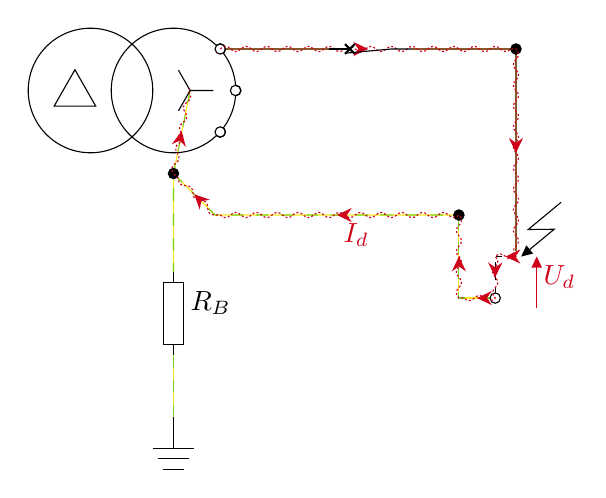
\begin{tikzpicture}[x=0.75pt,y=0.75pt,yscale=-1,xscale=1]
%uncomment if require: \path (0,251); %set diagram left start at 0, and has height of 251

%Straight Lines [id:da9415376086031365] 
\draw [color={rgb, 255:red, 0; green, 0; blue, 0 }  ,draw opacity=1 ] [dash pattern={on 2.25pt off 2.25pt}]  (242.5,132.5) -- (242.5,115) -- (252.5,115) ;
%Straight Lines [id:da5104591094158853] 
\draw [color={rgb, 255:red, 248; green, 231; blue, 28 }  ,draw opacity=1 ]   (87.5,75) -- (107.5,95) -- (225,95) ;
%Straight Lines [id:da1966201814177917] 
\draw [color={rgb, 255:red, 126; green, 211; blue, 33 }  ,draw opacity=1 ] [dash pattern={on 4.5pt off 4.5pt}]  (87.5,75) -- (107.5,95) -- (225,95) ;
%Straight Lines [id:da3955266461919331] 
\draw [color={rgb, 255:red, 248; green, 231; blue, 28 }  ,draw opacity=1 ]   (87.5,162.5) -- (87.5,192.5) ;
%Straight Lines [id:da18836033833143995] 
\draw [color={rgb, 255:red, 248; green, 231; blue, 28 }  ,draw opacity=1 ]   (240,135) -- (225,135) -- (225,95) ;
%Straight Lines [id:da17249205616306007] 
\draw [color={rgb, 255:red, 139; green, 87; blue, 42 }  ,draw opacity=1 ]   (112.5,15) -- (162.5,15) ;
%Straight Lines [id:da11309897556582038] 
\draw [color={rgb, 255:red, 248; green, 231; blue, 28 }  ,draw opacity=1 ]   (95.5,35) -- (87.5,75) -- (87.5,122.5) ;
%Straight Lines [id:da4238452834369957] 
\draw [color={rgb, 255:red, 126; green, 211; blue, 33 }  ,draw opacity=1 ] [dash pattern={on 4.5pt off 4.5pt}]  (95.5,35) -- (87.5,75) -- (87.5,122.5) ;
%Straight Lines [id:da07337279365918903] 
\draw [color={rgb, 255:red, 139; green, 87; blue, 42 }  ,draw opacity=1 ]   (202.5,15) -- (252.5,15) ;
%Shape: Path Data [id:dp3633653751506416] 
\draw   (112.5,55) .. controls (112.5,56.38) and (111.38,57.5) .. (110,57.5) .. controls (109.29,57.5) and (108.65,57.2) .. (108.19,56.72) .. controls (102.81,61.85) and (95.52,65) .. (87.5,65) .. controls (70.93,65) and (57.5,51.57) .. (57.5,35) .. controls (57.5,18.43) and (70.93,5) .. (87.5,5) .. controls (95.52,5) and (102.81,8.15) .. (108.19,13.28) .. controls (108.65,12.8) and (109.29,12.5) .. (110,12.5) .. controls (111.38,12.5) and (112.5,13.62) .. (112.5,15) .. controls (112.5,15.82) and (112.11,16.54) .. (111.5,17) .. controls (114.8,21.39) and (116.92,26.71) .. (117.4,32.5) .. controls (117.43,32.5) and (117.47,32.5) .. (117.5,32.5) .. controls (118.88,32.5) and (120,33.62) .. (120,35) .. controls (120,36.38) and (118.88,37.5) .. (117.5,37.5) .. controls (117.47,37.5) and (117.43,37.5) .. (117.4,37.5) .. controls (116.92,43.29) and (114.8,48.61) .. (111.5,53) .. controls (112.11,53.46) and (112.5,54.18) .. (112.5,55) -- cycle ;
%Shape: Circle [id:dp8103241388904666] 
\draw   (17.5,35) .. controls (17.5,18.43) and (30.93,5) .. (47.5,5) .. controls (64.07,5) and (77.5,18.43) .. (77.5,35) .. controls (77.5,51.57) and (64.07,65) .. (47.5,65) .. controls (30.93,65) and (17.5,51.57) .. (17.5,35) -- cycle ;
%Shape: Triangle [id:dp1236855376591316] 
\draw   (40,25) -- (30,42.5) -- (50,42.5) -- cycle ;
%Shape: Star [id:dp7604780706337534] 
\draw   (106.75,35) -- (95.5,35) -- (89.88,44.81) -- (95.5,35) -- (89.88,25.19) -- (95.5,35) -- cycle ;
%Shape: Circle [id:dp9987526738268633] 
\draw   (107.5,15) .. controls (107.5,13.62) and (108.62,12.5) .. (110,12.5) .. controls (111.38,12.5) and (112.5,13.62) .. (112.5,15) .. controls (112.5,16.38) and (111.38,17.5) .. (110,17.5) .. controls (108.62,17.5) and (107.5,16.38) .. (107.5,15) -- cycle ;
%Shape: Circle [id:dp06603296247595714] 
\draw   (114.9,35) .. controls (114.9,33.62) and (116.02,32.5) .. (117.4,32.5) .. controls (118.78,32.5) and (119.9,33.62) .. (119.9,35) .. controls (119.9,36.38) and (118.78,37.5) .. (117.4,37.5) .. controls (116.02,37.5) and (114.9,36.38) .. (114.9,35) -- cycle ;
%Shape: Circle [id:dp9864995024391362] 
\draw   (107.5,55) .. controls (107.5,53.62) and (108.62,52.5) .. (110,52.5) .. controls (111.38,52.5) and (112.5,53.62) .. (112.5,55) .. controls (112.5,56.38) and (111.38,57.5) .. (110,57.5) .. controls (108.62,57.5) and (107.5,56.38) .. (107.5,55) -- cycle ;

%Straight Lines [id:da23296631733343887] 
\draw [color={rgb, 255:red, 139; green, 87; blue, 42 }  ,draw opacity=1 ]   (252.5,112.5) -- (252.5,17.5) ;
%Straight Lines [id:da04537703273022686] 
\draw [color={rgb, 255:red, 126; green, 211; blue, 33 }  ,draw opacity=1 ] [dash pattern={on 4.5pt off 4.5pt}]  (240,135) -- (225,135) -- (225,95) ;
%Straight Lines [id:da014129266039552002] 
\draw    (87.5,192.5) -- (87.5,207.5) ;
%Straight Lines [id:da0064749529617041945] 
\draw    (77.5,207.5) -- (97.5,207.5) ;
%Straight Lines [id:da15495544426671526] 
\draw    (80,212.5) -- (95,212.5) ;
%Straight Lines [id:da9920646299152576] 
\draw    (82.5,217.5) -- (92.5,217.5) ;

%Straight Lines [id:da3741789060346865] 
\draw [color={rgb, 255:red, 126; green, 211; blue, 33 }  ,draw opacity=1 ] [dash pattern={on 4.5pt off 4.5pt}]  (87.5,162.5) -- (87.5,192.5) ;
%Straight Lines [id:da7734223518041439] 
\draw    (87.5,157.5) -- (87.5,162.5) ;
%Shape: Rectangle [id:dp997793865821069] 
\draw   (92.5,127.5) -- (92.5,157.5) -- (82.5,157.5) -- (82.5,127.5) -- cycle ;
%Straight Lines [id:da3149495431277475] 
\draw    (87.5,122.5) -- (87.5,127.5) ;

%Shape: Circle [id:dp16804091145958433] 
\draw  [fill={rgb, 255:red, 0; green, 0; blue, 0 }  ,fill opacity=1 ] (250,15) .. controls (250,13.62) and (251.12,12.5) .. (252.5,12.5) .. controls (253.88,12.5) and (255,13.62) .. (255,15) .. controls (255,16.38) and (253.88,17.5) .. (252.5,17.5) .. controls (251.12,17.5) and (250,16.38) .. (250,15) -- cycle ;
%Shape: Circle [id:dp448433802683451] 
\draw  [fill={rgb, 255:red, 255; green, 255; blue, 255 }  ,fill opacity=1 ] (240,135) .. controls (240,133.62) and (241.12,132.5) .. (242.5,132.5) .. controls (243.88,132.5) and (245,133.62) .. (245,135) .. controls (245,136.38) and (243.88,137.5) .. (242.5,137.5) .. controls (241.12,137.5) and (240,136.38) .. (240,135) -- cycle ;
%Shape: Circle [id:dp727181862391113] 
\draw  [fill={rgb, 255:red, 0; green, 0; blue, 0 }  ,fill opacity=1 ] (85,75) .. controls (85,73.62) and (86.12,72.5) .. (87.5,72.5) .. controls (88.88,72.5) and (90,73.62) .. (90,75) .. controls (90,76.38) and (88.88,77.5) .. (87.5,77.5) .. controls (86.12,77.5) and (85,76.38) .. (85,75) -- cycle ;
%Shape: Circle [id:dp14350658403367889] 
\draw  [fill={rgb, 255:red, 0; green, 0; blue, 0 }  ,fill opacity=1 ] (222.5,95) .. controls (222.5,93.62) and (223.62,92.5) .. (225,92.5) .. controls (226.38,92.5) and (227.5,93.62) .. (227.5,95) .. controls (227.5,96.38) and (226.38,97.5) .. (225,97.5) .. controls (223.62,97.5) and (222.5,96.38) .. (222.5,95) -- cycle ;
%Straight Lines [id:da09996473378362858] 
\draw [color={rgb, 255:red, 208; green, 2; blue, 27 }  ,draw opacity=1 ] [dash pattern={on 0.75pt off 0.75pt}]  (110,15) .. controls (111.67,13.33) and (113.33,13.33) .. (115,15) .. controls (116.67,16.67) and (118.33,16.67) .. (120,15) .. controls (121.67,13.33) and (123.33,13.33) .. (125,15) .. controls (126.67,16.67) and (128.33,16.67) .. (130,15) .. controls (131.67,13.33) and (133.33,13.33) .. (135,15) .. controls (136.67,16.67) and (138.33,16.67) .. (140,15) .. controls (141.67,13.33) and (143.33,13.33) .. (145,15) .. controls (146.67,16.67) and (148.33,16.67) .. (150,15) .. controls (151.67,13.33) and (153.33,13.33) .. (155,15) .. controls (156.67,16.67) and (158.33,16.67) .. (160,15) .. controls (161.67,13.33) and (163.33,13.33) .. (165,15) .. controls (166.67,16.67) and (168.33,16.67) .. (170,15) .. controls (171.67,13.33) and (173.33,13.33) .. (175,15) .. controls (176.67,16.67) and (178.33,16.67) .. (180,15) .. controls (181.67,13.33) and (183.33,13.33) .. (185,15) .. controls (186.67,16.67) and (188.33,16.67) .. (190,15) .. controls (191.67,13.33) and (193.33,13.33) .. (195,15) .. controls (196.67,16.67) and (198.33,16.67) .. (200,15) .. controls (201.67,13.33) and (203.33,13.33) .. (205,15) .. controls (206.67,16.67) and (208.33,16.67) .. (210,15) .. controls (211.67,13.33) and (213.33,13.33) .. (215,15) .. controls (216.67,16.67) and (218.33,16.67) .. (220,15) .. controls (221.67,13.33) and (223.33,13.33) .. (225,15) .. controls (226.67,16.67) and (228.33,16.67) .. (230,15) .. controls (231.67,13.33) and (233.33,13.33) .. (235,15) .. controls (236.67,16.67) and (238.33,16.67) .. (240,15) .. controls (241.67,13.33) and (243.33,13.33) .. (245,15) .. controls (246.67,16.67) and (248.33,16.67) .. (250,15) -- (252.5,15) -- (252.5,15) .. controls (254.17,16.67) and (254.17,18.33) .. (252.5,20) .. controls (250.83,21.67) and (250.83,23.33) .. (252.5,25) .. controls (254.17,26.67) and (254.17,28.33) .. (252.5,30) .. controls (250.83,31.67) and (250.83,33.33) .. (252.5,35) .. controls (254.17,36.67) and (254.17,38.33) .. (252.5,40) .. controls (250.83,41.67) and (250.83,43.33) .. (252.5,45) .. controls (254.17,46.67) and (254.17,48.33) .. (252.5,50) .. controls (250.83,51.67) and (250.83,53.33) .. (252.5,55) .. controls (254.17,56.67) and (254.17,58.33) .. (252.5,60) .. controls (250.83,61.67) and (250.83,63.33) .. (252.5,65) .. controls (254.17,66.67) and (254.17,68.33) .. (252.5,70) .. controls (250.83,71.67) and (250.83,73.33) .. (252.5,75) .. controls (254.17,76.67) and (254.17,78.33) .. (252.5,80) .. controls (250.83,81.67) and (250.83,83.33) .. (252.5,85) .. controls (254.17,86.67) and (254.17,88.33) .. (252.5,90) .. controls (250.83,91.67) and (250.83,93.33) .. (252.5,95) .. controls (254.17,96.67) and (254.17,98.33) .. (252.5,100) .. controls (250.83,101.67) and (250.83,103.33) .. (252.5,105) .. controls (254.17,106.67) and (254.17,108.33) .. (252.5,110) .. controls (250.83,111.67) and (250.83,113.33) .. (252.5,115) -- (252.5,115) .. controls (250.83,116.67) and (249.17,116.67) .. (247.5,115) .. controls (245.83,113.33) and (244.17,113.33) .. (242.5,115) -- (242.5,115) .. controls (244.17,116.67) and (244.17,118.33) .. (242.5,120) .. controls (240.83,121.67) and (240.83,123.33) .. (242.5,125) .. controls (244.17,126.67) and (244.17,128.33) .. (242.5,130) .. controls (240.83,131.67) and (240.83,133.33) .. (242.5,135) -- (242.5,135) -- (242.5,135) .. controls (240.83,136.67) and (239.17,136.67) .. (237.5,135) .. controls (235.83,133.33) and (234.17,133.33) .. (232.5,135) .. controls (230.83,136.67) and (229.17,136.67) .. (227.5,135) -- (225,135) -- (225,135) .. controls (223.33,133.33) and (223.33,131.67) .. (225,130) .. controls (226.67,128.33) and (226.67,126.67) .. (225,125) .. controls (223.33,123.33) and (223.33,121.67) .. (225,120) .. controls (226.67,118.33) and (226.67,116.67) .. (225,115) .. controls (223.33,113.33) and (223.33,111.67) .. (225,110) .. controls (226.67,108.33) and (226.67,106.67) .. (225,105) .. controls (223.33,103.33) and (223.33,101.67) .. (225,100) .. controls (226.67,98.33) and (226.67,96.67) .. (225,95) -- (225,95) -- (225,95) .. controls (223.33,96.67) and (221.67,96.67) .. (220,95) .. controls (218.33,93.33) and (216.67,93.33) .. (215,95) .. controls (213.33,96.67) and (211.67,96.67) .. (210,95) .. controls (208.33,93.33) and (206.67,93.33) .. (205,95) .. controls (203.33,96.67) and (201.67,96.67) .. (200,95) .. controls (198.33,93.33) and (196.67,93.33) .. (195,95) .. controls (193.33,96.67) and (191.67,96.67) .. (190,95) .. controls (188.33,93.33) and (186.67,93.33) .. (185,95) .. controls (183.33,96.67) and (181.67,96.67) .. (180,95) .. controls (178.33,93.33) and (176.67,93.33) .. (175,95) .. controls (173.33,96.67) and (171.67,96.67) .. (170,95) .. controls (168.33,93.33) and (166.67,93.33) .. (165,95) .. controls (163.33,96.67) and (161.67,96.67) .. (160,95) .. controls (158.33,93.33) and (156.67,93.33) .. (155,95) .. controls (153.33,96.67) and (151.67,96.67) .. (150,95) .. controls (148.33,93.33) and (146.67,93.33) .. (145,95) .. controls (143.33,96.67) and (141.67,96.67) .. (140,95) .. controls (138.33,93.33) and (136.67,93.33) .. (135,95) .. controls (133.33,96.67) and (131.67,96.67) .. (130,95) .. controls (128.33,93.33) and (126.67,93.33) .. (125,95) .. controls (123.33,96.67) and (121.67,96.67) .. (120,95) .. controls (118.33,93.33) and (116.67,93.33) .. (115,95) .. controls (113.33,96.67) and (111.67,96.67) .. (110,95) -- (107.5,95) -- (107.5,95) .. controls (105.14,95) and (103.96,93.82) .. (103.96,91.46) .. controls (103.96,89.11) and (102.78,87.93) .. (100.43,87.93) .. controls (98.07,87.93) and (96.89,86.75) .. (96.89,84.39) .. controls (96.89,82.04) and (95.71,80.86) .. (93.36,80.86) .. controls (91,80.86) and (89.82,79.68) .. (89.82,77.32) -- (87.5,75) -- (87.5,75) .. controls (86.17,73.05) and (86.48,71.42) .. (88.43,70.09) .. controls (90.38,68.76) and (90.69,67.12) .. (89.36,65.17) .. controls (88.03,63.22) and (88.34,61.59) .. (90.29,60.26) .. controls (92.24,58.93) and (92.54,57.3) .. (91.21,55.35) .. controls (89.88,53.4) and (90.19,51.77) .. (92.14,50.44) .. controls (94.09,49.11) and (94.4,47.47) .. (93.07,45.52) .. controls (91.74,43.57) and (92.05,41.94) .. (94,40.61) .. controls (95.95,39.28) and (96.26,37.65) .. (94.93,35.7) -- (95.25,34) -- (95.25,34) ;
\draw [shift={(181.25,15)}, rotate = 180] [fill={rgb, 255:red, 208; green, 2; blue, 27 }  ,fill opacity=1 ][line width=0.08]  [draw opacity=0] (7.14,-3.43) -- (0,0) -- (7.14,3.43) -- (4.74,0) -- cycle    ;
\draw [shift={(252.5,65)}, rotate = 270] [fill={rgb, 255:red, 208; green, 2; blue, 27 }  ,fill opacity=1 ][line width=0.08]  [draw opacity=0] (7.14,-3.43) -- (0,0) -- (7.14,3.43) -- (4.74,0) -- cycle    ;
\draw [shift={(247.5,115)}, rotate = 360] [fill={rgb, 255:red, 208; green, 2; blue, 27 }  ,fill opacity=1 ][line width=0.08]  [draw opacity=0] (7.14,-3.43) -- (0,0) -- (7.14,3.43) -- (4.74,0) -- cycle    ;
\draw [shift={(242.5,125)}, rotate = 270] [fill={rgb, 255:red, 208; green, 2; blue, 27 }  ,fill opacity=1 ][line width=0.08]  [draw opacity=0] (7.14,-3.43) -- (0,0) -- (7.14,3.43) -- (4.74,0) -- cycle    ;
\draw [shift={(233.75,135)}, rotate = 360] [fill={rgb, 255:red, 208; green, 2; blue, 27 }  ,fill opacity=1 ][line width=0.08]  [draw opacity=0] (7.14,-3.43) -- (0,0) -- (7.14,3.43) -- (4.74,0) -- cycle    ;
\draw [shift={(225,115)}, rotate = 450] [fill={rgb, 255:red, 208; green, 2; blue, 27 }  ,fill opacity=1 ][line width=0.08]  [draw opacity=0] (7.14,-3.43) -- (0,0) -- (7.14,3.43) -- (4.74,0) -- cycle    ;
\draw [shift={(166.25,95)}, rotate = 360] [fill={rgb, 255:red, 208; green, 2; blue, 27 }  ,fill opacity=1 ][line width=0.08]  [draw opacity=0] (7.14,-3.43) -- (0,0) -- (7.14,3.43) -- (4.74,0) -- cycle    ;
\draw [shift={(97.5,85)}, rotate = 405] [fill={rgb, 255:red, 208; green, 2; blue, 27 }  ,fill opacity=1 ][line width=0.08]  [draw opacity=0] (7.14,-3.43) -- (0,0) -- (7.14,3.43) -- (4.74,0) -- cycle    ;
\draw [shift={(91.38,54.5)}, rotate = 460.7] [fill={rgb, 255:red, 208; green, 2; blue, 27 }  ,fill opacity=1 ][line width=0.08]  [draw opacity=0] (7.14,-3.43) -- (0,0) -- (7.14,3.43) -- (4.74,0) -- cycle    ;
%Shape: Boxed Line [id:dp3673372749832414] 
\draw    (274.27,88.83) -- (258.39,101.97) -- (270.89,101.86) -- (257.31,113.09) ;
\draw [shift={(255,115)}, rotate = 320.40999999999997] [fill={rgb, 255:red, 0; green, 0; blue, 0 }  ][line width=0.08]  [draw opacity=0] (5.36,-2.57) -- (0,0) -- (5.36,2.57) -- cycle    ;
%Straight Lines [id:da5575509867036751] 
\draw    (170.5,17) -- (192.5,15) -- (202.5,15) ;
%Straight Lines [id:da508912305096757] 
\draw    (172.5,15) -- (162.5,15) ;
\draw [shift={(172.5,15)}, rotate = 225] [color={rgb, 255:red, 0; green, 0; blue, 0 }  ][line width=0.75]    (-3.35,0) -- (3.35,0)(0,3.35) -- (0,-3.35)   ;

%Straight Lines [id:da16958097231268054] 
\draw [color={rgb, 255:red, 208; green, 2; blue, 27 }  ,draw opacity=1 ]   (262.5,118) -- (262.5,140) ;
\draw [shift={(262.5,115)}, rotate = 90] [fill={rgb, 255:red, 208; green, 2; blue, 27 }  ,fill opacity=1 ][line width=0.08]  [draw opacity=0] (5.36,-2.57) -- (0,0) -- (5.36,2.57) -- cycle    ;


% Text Node
\draw (94.5,130.5) node [anchor=north west][inner sep=0.75pt]   [align=left] {$R_B$};
% Text Node
\draw (168.25,98) node [anchor=north west][inner sep=0.75pt]  [color={rgb, 255:red, 208; green, 2; blue, 27 }  ,opacity=1 ] [align=left] {$I_d$};
% Text Node
\draw (264.5,118) node [anchor=north west][inner sep=0.75pt]  [color={rgb, 255:red, 208; green, 2; blue, 27 }  ,opacity=1 ] [align=left] {$U_d$};


\end{tikzpicture}

\end{figure}

%\end{document}



Pour calculer le courant de défaut $I_d$, il existe trois méthode, mais ne sera détaillé dans ce chapitre que la première (plus de précisions sur les deux autres méthode \superref{ann:schema_tn}) :
\begin{itemize}
\item Méthode conventionnelle\,;
\item Méthode des impédances\,;
\item Méthode de composition.
\end{itemize}

\section{Méthode de dimensionnement conventionnelle des protections et des sections de conducteurs\label{sec:schema_tn_methode_conventionnelle}}

Contrairement au SLT TT, il ne faut pas tenir compte de la \emph{résistance de défaut} $R_d$ qui prend en compte la nature du défaut d'isolement (franc ou non-franc) et la résistance de la carcasse métallique car il s'agit d'un court-circuit et elle sera donc très faible.\\
$I_d$ s'apparente donc à un courant de court-circuit et son calcul est basé sur l'hypothèse que la tension de défaut reste supérieur à 80\% ou plus de la tension nominale simple. Cette valeur est issue d'une estimation de la chute de tension due à l'ensemble des impédances en amont de la protection du circuit en défaut. Elle est utilisée, avec l'impédance de la boucle de circuit, pour calculer ce courant de court-circuit.\\ 

Ce facteur est calculé par l'estimation de la chute de tension due à l'ensemble des impédances en amont de cette origine. Dans une majorité des types de pose, les réactances inductive interne et entres les conducteurs sont négligées, ce qui revient à ne considérer que les résistances des conducteurs dans les calculs d'intensité de court-circuit. Cette approximation est considérée comme valable pour les sections de câble jusqu'à \SI{120}{\square\milli\meter}. Au-dessus de cette section, la résistance $R$ des conducteurs est augmentée selon le tableau ci-dessous :

\begin{table}[H]
\caption{Section des conducteurs (schéma TN / méthode conventionnelle)}
\begin{tabularx}{0.8\linewidth}{Q K@{${\enspace{}}+{\enspace{}}$}I}
\toprule
\multicolumn{2}{c}{\thead{Section des conducteurs}} & \multicolumn{2}{c}{\thead{Ajustement de la résistance en \si{\ohm}}} \\
\midrule
S & \SI{150}{\square\milli\meter} & R & 15\% \\
S & \SI{185}{\square\milli\meter} & R & 20\% \\
S & \SI{240}{\square\milli\meter} & R & 25\% \\
\bottomrule
\end{tabularx}
\end{table}

\begin{formule}{Courant de défaut $I_d$ en schéma TN selon la méthode conventionnelle}{courant_defaut_tn_conventionnel}
\begin{align*}
		I_d &= \frac{0,8 \times U_{0}}{R_{PE}+R_{ph}} \\
		I_d &= \frac{0,8 \times U_{0}}{Z_{c}}
\end{align*}

\begin{textvariables}
U_{0}						& tension							& volt			& \volt					& 	Tension nominale simple \\
0,8							& facteur							& 					& 	/						& 	facteur d'approximation de la tension de défaut $U_d$ \\
R_{PE}						& résistance						& ohm			& \ohm					& 	Résistance du conducteur de phase traversé par un courant de défaut $I_d$	\\
R_{ph}						& résistance						& ohm			& \ohm					& 	Résistance du conducteur PE traversé par un courant de défaut $I_d$ \\
Z_{c}						& impédance						& ohm			& \ohm					& Impédance de boucle du circuit en défaut (selon la méthode conventionnelle)\\
\end{textvariables}
\end{formule}

Le courant de défaut $I_d$ fera alors apparaître une \emph{tension de défaut} $U_d$ entre la masse métallique et la terre :

\begin{formule}{Tension de défaut $U_d$ en schéma TN selon la méthode conventionnelle}{}
\begin{align*}
		U_d &= R_{PE} \times I_{d}
\end{align*}

\begin{textvariables}
R_{PE}						& résistance						& ohm			& \ohm					& 	Résistance du conducteur PE traversé par un courant de défaut $I_d$	\\
I_{d}							& intensité							& ampère		& \ampere				& 	Courant de défaut d'isolement \\
\end{textvariables}
\end{formule}

La tension de défaut $U_d$ dans le cas d'un défaut d'isolement en régime TN est \emph{élevée} et donc \emph{dangereuse} si elle est supportée trop longtemps. La norme NF C15-100 a défini des temps de coupure maximum à respecter :

%--------------------------------------
%ELECTROTECHNIQUE - SCHEMA DE LIAISON A LA TERRE
%--------------------------------------

%utiliser les environnement \begin{comment} \end{comment} pour mettre en commentaire le préambule une fois la programmation appelée dans le document maître (!ne pas oublier de mettre en commentaire \end{document}!)

\begin{comment}

\documentclass[a4paper, 11pt, twoside, fleqn]{memoir}

\usepackage{AOCDTF}

\marqueurchapitre
\decoupagechapitre{1} %juste pour éviter les erreurs lors de la compilation des sous-programmations (passera en commentaire)

%lien d'édition des figures Tikz sur le site mathcha.io (rajouter le lien d'une modification effectuée sur la figure tikz avec le nom du modificateur car il n'y a qu'un lien par compte)

%lien éditeur Bruno Douchy : https://www.mathcha.io/editor/zjygnFElSdyhJ72e3zT5ZgqwBT4DKnovswpXn1q

%--------------------------------------
%corps du document
%--------------------------------------

\begin{document} %corps du document
	\openleft %début de chapitre à gauche

\end{comment}

\begin{table}[H]
\caption{Temps de coupure maximal des disjoncteurs en schéma TN\label{tab:schema_tn_temps_coupure}}
\begin{tabularx}{\textwidth}{C C C}
\toprule
\multirow[c]{2}{*}{\thead{Réseaux usuels}} & \multicolumn{2}{c}{\thead{Temps de coupure maximal en \si{\milli\second}}}\\
\cmidrule(lr){2-3} 
	& $U_{L}=\SI{50}{\volt}$ 	& 			$U_{L}=\SI{25}{\volt}$  \\
\midrule
\SI{127}{\volt}/\SI{230}{\volt}		& 800		& 350 \\
\SI{230}{\volt}/\SI{400}{\volt}		& 400		& 200 \\
\SI{400}{\volt}/\SI{690}{\volt}		& 200		& 50 \\
\SI{690}{\volt}/\SI{1000}{\volt}	& 100		& 20 \\
\bottomrule 
\end{tabularx}
\end{table}

%\end{document}



\begin{formule}{Seuil de réglage du disjoncteur $I_m$ en schéma TN}{}
\begin{align*}
		I_{m} &> I_{d}
\end{align*}

\begin{textvariables}
I_{m}						& intensité							& ampère			& \ampere					& 	Intensité de seuil de déclenchement de la protection magnétique du disjoncteur \\
\end{textvariables}
\end{formule}

On peut calculer la longueur maximale d'un circuit d'une installation en schéma TN par la formule suivante :\\

\begin{formule}{Longueur maximale d'un circuit $L_{max}$}{schema_tn_longueur_max_circuit}
\begin{align*}
		L_{max} &= \frac{0,8 \times U_{0} \times S_{ph}}{\rho \times (1+m) \times I_m}\\
		m &= \frac{S_{ph}}{S_{PE}}
\end{align*}
\begin{textvariables}
I_{m}						& intensité							& ampère			& \ampere							& 	Intensité de seuil de déclenchement de la protection magnétique du disjoncteur \\
U_{0}						& tension							& volt				& \volt								& 	Tension nominale simple \\
S_{ph}						& section							& millimètre\up{2}		& \si{\square\milli\meter}	& 	Section du conducteur de phase traversé par un courant de défaut $I_d$ \\
S_{PE}						& section							& millimètre\up{2}		& \si{\square\milli\meter}	& 	Section du conducteur PE traversé par un courant de défaut $I_d$ \\
\rho							& résistivité						& 									& /	& 	Résistivité du conducteur (selon la température et le matériau choisi) :
\begin{tabdescription}
\item[aluminium :] \SI{37.6e-3}{\ohm\square\milli\meter\per\meter}
\item[cuivre :] \SI{22.5e-3}{\ohm\square\milli\meter\per\meter}
\end{tabdescription}\\
m								& facteur		& 			& /										& Facteur de correction à appliquer aux valeurs données dans les abaques de détermination des longueurs selon la section et l'intensité de déclenchement (\superref{subsubsec:facteur_correction_m}) 	 \\
\end{textvariables}
\end{formule}


Pour vérifier rapidement un dimensionnement, les constructeurs de protections ont établis des abaques permettant de déterminer rapidement les longueurs maximale des conducteurs selon l'intensité, la section des conducteurs ou en encore les réglages du seuil de courant de déclenchement du disjoncteur ou encore le type de disjoncteurs. Ces abaques sont issus des norme IEC 60947-2\supercite{IEC:60947-2-2016} et IEC 60898\supercite{IEC:60898-2015}, qui concernent respectivement les disjoncteurs industriels et domestiques. Ils sont détaillés dans l'annexe \superref{ann:schema_tn}.

\begin{exemple}{Calcul du courant de défaut $I_d$ en schéma TN selon la méthode conventionnelle}{}
Si on considère que les conducteurs sont en cuivre, que $U_{0}=\SI{230}{\volt}$, que $L_{ph}=\SI{50}{\meter}$ et est équivalent à $L_{PE}$, que $S_{ph}=\SI{35}{\square\milli\meter}$ et est équivalent à  $S_{PE}$, on peut déduire que le courant de défaut $I_d$ vaut :
\begin{align*}
		Z_{c}	&= 2 \times \rho \times \frac{L}{S}  								& 			I_d		&= \frac{U_0 \times 0,8}{Z_c} \\
					&= 2 \times 22.5 \times 10^{-3} \times \frac{50}{35} 	&						&= \frac{230 \times 0,8}{64,3 \times 10^{-3}} \\
					&= \SI{64,3}{\milli\ohm}						 						& 						&= \SI{2816}{\ampere}
\end{align*}
\end{exemple}

\begin{exemple}{Calcul de la longueur maximale des conducteurs $L_{max}$ en schéma TN selon la méthode conventionnelle}{}
Si on considère que les conducteurs sont en cuivre, que $U_{0}=\SI{230}{\volt}$, que $L{ph}=\SI{50}{\meter}$ et est équivalent à $L{PE}$, que $S_{ph}=\SI{35}{\square\milli\meter}$ et est équivalent à  $S_{PE}$, on peut déduire que le courant de défaut $I_d$ vaut :
\begin{align*}
		Z_{c}	&= 2 \times \rho \times \frac{L}{S}  								& 			I_d		&= \frac{U_0 \times 0,8}{Z_c} \\
					&= 2 \times 22.5 \times 10^{-3} \times \frac{50}{35} 			&				&= \frac{230 \times 0,8}{64,3e \times 10^{-3}} \\
					&= \SI{64,3}{\milli\ohm}						 						& 						&= \SI{2816}{\ampere}
\end{align*}

Il convient de croiser cette valeur de $I_d$ avec les valeurs du seuil de déclenchement du disjoncteur Instantané et Court-retard et leurs temps de coupures respectifs (voir \superref{tab:schema_tn_temps_coupure}) pour valider le dimensionnement et le choix de la protection.
\end{exemple}

\section{Protection avec des DDR en schéma TN}

La protection des circuits à l'aide de DDR en schéma TN est formellement interdite en schéma TN-C car le conducteur PE ne peut pas être sectionné. En schéma TN-C-S, son utilisation implique forcément que les conducteurs PE et N soient séparés en amont du DDR.\\

Les DDR en schéma TN-S sont requis lorsque :
\begin{itemize}
\item l'impédance de la boucle de défaut $Z_c$ n'est pas précisément calculable\,;
\item le courant de défaut est trop faible pour que la protection détecte le défaut comme s'apparentant à un court-circuit dans le temps de déconnexion requis.
\end{itemize}

Un DDR se déclenchant avec un courant de déclenchement de l'ordre que quelques ampères maximum, il convient bien à un circuit terminal d'une installation BT conséquente en schéma TN.

\end{document}

	%--------------------------------------
%ELECTROTECHNIQUE - SCHEMA DE LIAISON A LA TERRE
%--------------------------------------

%utiliser les environnement \begin{comment} \end{comment} pour mettre en commentaire le préambule une fois la programmation appelée dans le document maître (!ne pas oublier de mettre en commentaire \end{document}!)

\begin{comment}

\documentclass[a4paper, 11pt, twoside, fleqn]{memoir}

\usepackage{AOCDTF}

\marqueurchapitre
\decoupagechapitre{1} %juste pour éviter les erreurs lors de la compilation des sous-programmations (passera en commentaire)

%--------------------------------------
%corps du document
%--------------------------------------

\begin{document} %corps du document
	\openleft %début de chapitre à gauche

\end{comment}

\chapter{Schéma Impédant-Terre\label{chap:schema_it}}
\ChapFrame

\section{Caractéristiques générales}

\begin{definition}{Schéma IT}{}
Schéma de liaison à la terre dans lequel le prise de terre du neutre du transformateur et la prise de terre des masses métalliques sont raccordées à la terre selon quatre variantes différentes :
\begin{description}
\item [Neutre :] isolé du point neutre du transformateur HT/BT (complètement isolé ou via une \emph{impédance de limitation})\,;
\item [Masses :] reliées à la terre (interconnectées ou individuellement).
\end{description}
\end{definition}

\begin{table}[H]
\caption{Détail sur les variantes de branchement en schéma IT}
\begin{tabularx}{\linewidth}{XXXX}
\toprule
\multicolumn{2}{c}{\thead{Neutre transformateur HT/BT}} & \multicolumn{2}{c}{\thead{Masses conductrices}} \\
\cmidrule(lr){1-2} 	\cmidrule(lr){3-4}
\thead{Isolé ($Z_{res}$)}	& \thead{Impédant ($Z_{N}$)}	& \thead{Interconnectées}	& \thead{Individuelles} \\
\midrule
Neutre du transformateur pas raccordé du tout. Terme \og isolé \fg{} à nuancer car l'installation électrique en aval du transformateur HT/BT ne sera jamais complètement isolée par rapport à la terre. Il subsistera toujours un courant de défaut $I_d$ plus ou moins minime due à une impédance de fuite $Z_{res}$ présente dans tous les réseaux électriques (voir \superref{sec:isolation_installation_schema_it}).
& 
Neutre du transformateur raccordé à la prise de terre par une \emph{impédance de limitation} dont la valeur dépend de la fréquence de la tension :
\begin{compactitemize}
\item$F=\SI{50}{\hertz}$ : \SI{1500}{\ohm}\,;
\item$F=\SI{2,5}{\hertz}$ : \SI{2,5}{\ohm}.
\end{compactitemize}
Cette impédance fixe donc une différence de potentiel définie entre le neutre et la terre, elle est installée lorsque le réseau électrique est court et que l'impédance de fuite $Z_{res}$ est élevée.
&
Masses \emph{interconnectées} au moyen d'un conducteur PE et raccordées à la terre au niveau du transformateur HT/BT. Raccordement similaire au schéma TN, à la différence que le neutre du transformateur n'est pas raccordé au conducteur PE et à la terre.
&
Masses mise à la terre \emph{individuellement} ou par groupe à des prises de terre propres. Type de raccordement similaire au schéma TT avec installation de DDR en tête de chaque circuit. \\
\bottomrule
\end{tabularx}
\end{table}

Il s'agit d'un SLT un peu plus atypique ayant pour but d'assurer une \emph{continuité de service} à l'installation électrique malgré un \emph{premier défaut d'isolement} tout en assurant la protection des personnes contre les contacts indirects. Selon les quatre variantes de raccordement, le premier défaut entrainera un fonctionnement identique des protections mais à l'apparition d'un deuxième défaut entrainera un fonctionnement des protection différent.\\

Dans la pratique, le schéma IT présente les caractéristiques suivantes :
\begin{itemize}
\item continuité de service assurée après un premier défaut d'isolement\,;
\item contrôle permanent de l'isolement de l'installation par rapport à la terre avec signalisation de toute dépassement du seuil d'isolement défini à l'aide d'un Contrôleur Permanent d'Isolement (CPI)\,;
\item protection du neutre assurée\,;
\item raccordement possible d'un limiteur de tension (éclateur) entre la terre et le point neutre du transformateur HT/BT\,;
\item présence continue d'une équipe pour assurer rapidement la recherche du premier défaut d'isolement aussitôt signalé, facilitée avec du matériel de localisation automatique\,;
\item coupure automatique de l'installation dès l'apparition d'un second défaut d'isolement sur un conducteur actif différent de celui ou le premier défaut d'isolement est apparu.
\end{itemize}

Le courant de défaut du premier défaut d'isolement va dépendre de l'impédance de limitation du neutre et de l'état d'isolement de l'installation électrique. Pour toutefois protéger les personnes, il doit être suffisamment bas pour satisfaire la règle $I_{d} \times R_{A} \pm \SI{50}{\volt}$, de sorte à ce que la tension de défaut $U_d$ ne présente aucun danger.

\section{Isolation de l'installation électrique en schéma IT\label{sec:isolation_installation_schema_it}}

Dans le cas d'un schéma IT ou le neutre est isolé, l'isolement de l'installation de l'installation électrique n'est pas infini par rapport à la terre car les isolants ne présentent jamais une résistance infinie. Une résistance de fuite du de l'installation électrique apparaitra toujours et dépendra de plusieurs facteurs :
\begin{itemize}
\item nature des isolants (PVC, air\ldots)\,;
\item âge de l'installation
\item degré d'humidité\,;
\item longueur de l'installation.
\end{itemize}
Pour une installation neuve, on considère que la résistance de fuite est estimée à \SI{3,3}{\mega\ohm} pour \SI{1}{\kilo\meter} de réseau électrique.

\begin{formule}{Résistance de fuite du réseaux $R_{res}$ d'une installation neuve}{}
\begin{align*}
	R_{res} &= \frac{3,3}{n}
\end{align*} 
\begin{textvariables}
R_{res}						& résistance					& méga-ohm			& \mega\ohm							& 	Résistance de fuite du réseaux électrique \\
n								& 									& 							& /										& 	Nombre de \si{\kilo\meter} de réseaux électrique \\
\end{textvariables}
\end{formule}

%--------------------------------------
%ELECTROTECHNIQUE - SCHEMA DE LIAISON A LA TERRE
%--------------------------------------

%utiliser les environnement \begin{comment} \end{comment} pour mettre en commentaire le préambule une fois la programmation appelée dans le document maître (!ne pas oublier de mettre en commentaire \end{document}!)

\begin{comment}

\documentclass[a4paper, 11pt, twoside, fleqn]{memoir}

\usepackage{AOCDTF}

\marqueurchapitre
\decoupagechapitre{1} %juste pour éviter les erreurs lors de la compilation des sous-programmations (passera en commentaire)

%lien d'édition des figures Tikz sur le site mathcha.io (rajouter le lien d'une modification effectuée sur la figure tikz avec le nom du modificateur car il n'y a qu'un lien par compte)

%lien mathcha Bruno Douchy : https://www.mathcha.io/editor/Kxxn3cWBUm3T7ynYmWi4KY0P9H9d6v9qFLQyMEE

%--------------------------------------
%corps du document
%--------------------------------------

\begin{document} %corps du document
	\openleft %début de chapitre à gauche

\end{comment}


% Pattern Info
\begin{figure}[H]
\caption{Résistance de fuite $R_{res}$ d'un réseau électrique de plusieurs \si{\kilo\meter}}

% Pattern Info
 
\tikzset{
pattern size/.store in=\mcSize, 
pattern size = 5pt,
pattern thickness/.store in=\mcThickness, 
pattern thickness = 0.3pt,
pattern radius/.store in=\mcRadius, 
pattern radius = 1pt}
\makeatletter
\pgfutil@ifundefined{pgf@pattern@name@_sgw0g8yxt}{
\pgfdeclarepatternformonly[\mcThickness,\mcSize]{_sgw0g8yxt}
{\pgfqpoint{0pt}{0pt}}
{\pgfpoint{\mcSize+\mcThickness}{\mcSize+\mcThickness}}
{\pgfpoint{\mcSize}{\mcSize}}
{
\pgfsetcolor{\tikz@pattern@color}
\pgfsetlinewidth{\mcThickness}
\pgfpathmoveto{\pgfqpoint{0pt}{0pt}}
\pgfpathlineto{\pgfpoint{\mcSize+\mcThickness}{\mcSize+\mcThickness}}
\pgfusepath{stroke}
}}
\makeatother
\tikzset{every picture/.style={line width=0.75pt}} %set default line width to 0.75pt        

\begin{tikzpicture}[x=0.75pt,y=0.75pt,yscale=-1,xscale=1]
%uncomment if require: \path (0,327); %set diagram left start at 0, and has height of 327

%Straight Lines [id:da08009100326878149] 
\draw    (105,35) -- (210,35) ;
%Shape: Circle [id:dp3640107906362746] 
\draw   (2.5,35) .. controls (2.5,18.43) and (15.93,5) .. (32.5,5) .. controls (49.07,5) and (62.5,18.43) .. (62.5,35) .. controls (62.5,51.57) and (49.07,65) .. (32.5,65) .. controls (15.93,65) and (2.5,51.57) .. (2.5,35) -- cycle ;
%Straight Lines [id:da571377768464931] 
\draw    (30,232.5) -- (545,232.5) ;
%Straight Lines [id:da08045007432417306] 
\draw    (210,247.5) -- (210,262.5) ;
%Straight Lines [id:da4313577623259258] 
\draw    (200,262.5) -- (220,262.5) ;
%Straight Lines [id:da5912684771420953] 
\draw    (202.5,267.5) -- (217.5,267.5) ;
%Straight Lines [id:da13165123057200734] 
\draw    (205,272.5) -- (215,272.5) ;

%Straight Lines [id:da320941654963934] 
\draw    (210,217.5) -- (210,222.5) ;
%Shape: Rectangle [id:dp24059175551770873] 
\draw   (215,187.5) -- (215,217.5) -- (205,217.5) -- (205,187.5) -- cycle ;
%Straight Lines [id:da9352215304977288] 
\draw    (210,182.5) -- (210,187.5) ;

%Shape: Circle [id:dp5173960999636192] 
\draw   (45,35) .. controls (45,18.43) and (58.43,5) .. (75,5) .. controls (91.57,5) and (105,18.43) .. (105,35) .. controls (105,51.57) and (91.57,65) .. (75,65) .. controls (58.43,65) and (45,51.57) .. (45,35) -- cycle ;
%Straight Lines [id:da826385807465586] 
\draw    (140,45) -- (150,25) ;
\draw [shift={(150,25)}, rotate = 296.57] [color={rgb, 255:red, 0; green, 0; blue, 0 }  ][fill={rgb, 255:red, 0; green, 0; blue, 0 }  ][line width=0.75]      (0, 0) circle [x radius= 2.01, y radius= 2.01]   ;
%Straight Lines [id:da9637899679537502] 
\draw    (120,45) -- (130,25) ;
%Straight Lines [id:da6640472127950414] 
\draw    (115,45) -- (125,25) ;
%Straight Lines [id:da46557993038086076] 
\draw    (110,45) -- (120,25) ;

%Straight Lines [id:da33735776097392156] 
\draw    (210,222.5) -- (210,247.5) ;
%Straight Lines [id:da5122217943063542] 
\draw    (210,35) -- (210,182.5) ;
%Shape: Circle [id:dp05291492243843332] 
\draw  [fill={rgb, 255:red, 0; green, 0; blue, 0 }  ,fill opacity=1 ] (207.5,35) .. controls (207.5,33.62) and (208.62,32.5) .. (210,32.5) .. controls (211.38,32.5) and (212.5,33.62) .. (212.5,35) .. controls (212.5,36.38) and (211.38,37.5) .. (210,37.5) .. controls (208.62,37.5) and (207.5,36.38) .. (207.5,35) -- cycle ;
%Straight Lines [id:da6377337353392218] 
\draw    (212.5,35) -- (317.5,35) ;
%Straight Lines [id:da25115314727149973] 
\draw    (317.5,247.5) -- (317.5,262.5) ;
%Straight Lines [id:da901440360563758] 
\draw    (307.5,262.5) -- (327.5,262.5) ;
%Straight Lines [id:da7842646096579663] 
\draw    (310,267.5) -- (325,267.5) ;
%Straight Lines [id:da18808830899848483] 
\draw    (312.5,272.5) -- (322.5,272.5) ;

%Straight Lines [id:da49919296084643217] 
\draw    (317.5,217.5) -- (317.5,222.5) ;
%Shape: Rectangle [id:dp5156050966431545] 
\draw   (322.5,187.5) -- (322.5,217.5) -- (312.5,217.5) -- (312.5,187.5) -- cycle ;
%Straight Lines [id:da9531373030412352] 
\draw    (317.5,182.5) -- (317.5,187.5) ;

%Straight Lines [id:da8099985845539385] 
\draw    (247.5,45) -- (257.5,25) ;
\draw [shift={(257.5,25)}, rotate = 296.57] [color={rgb, 255:red, 0; green, 0; blue, 0 }  ][fill={rgb, 255:red, 0; green, 0; blue, 0 }  ][line width=0.75]      (0, 0) circle [x radius= 2.01, y radius= 2.01]   ;
%Straight Lines [id:da8087453766565224] 
\draw    (227.5,45) -- (237.5,25) ;
%Straight Lines [id:da3541011282357912] 
\draw    (222.5,45) -- (232.5,25) ;
%Straight Lines [id:da4838872480993197] 
\draw    (217.5,45) -- (227.5,25) ;

%Straight Lines [id:da6527379034333531] 
\draw    (317.5,222.5) -- (317.5,247.5) ;
%Straight Lines [id:da5530613085402983] 
\draw    (317.5,35) -- (317.5,182.5) ;
%Shape: Circle [id:dp25176527117973546] 
\draw  [fill={rgb, 255:red, 0; green, 0; blue, 0 }  ,fill opacity=1 ] (315,35) .. controls (315,33.62) and (316.12,32.5) .. (317.5,32.5) .. controls (318.88,32.5) and (320,33.62) .. (320,35) .. controls (320,36.38) and (318.88,37.5) .. (317.5,37.5) .. controls (316.12,37.5) and (315,36.38) .. (315,35) -- cycle ;
%Straight Lines [id:da18023630680839797] 
\draw    (320,35) -- (425,35) ;
%Straight Lines [id:da6476101136895756] 
\draw    (425,247.5) -- (425,262.5) ;
%Straight Lines [id:da4732182664219796] 
\draw    (415,262.5) -- (435,262.5) ;
%Straight Lines [id:da9789341071401707] 
\draw    (417.5,267.5) -- (432.5,267.5) ;
%Straight Lines [id:da9061441462289892] 
\draw    (420,272.5) -- (430,272.5) ;

%Straight Lines [id:da5168046359577328] 
\draw    (425,217.5) -- (425,222.5) ;
%Shape: Rectangle [id:dp6616267367458876] 
\draw   (430,187.5) -- (430,217.5) -- (420,217.5) -- (420,187.5) -- cycle ;
%Straight Lines [id:da5013364563135433] 
\draw    (425,182.5) -- (425,187.5) ;

%Straight Lines [id:da8467083023662558] 
\draw    (355,45) -- (365,25) ;
\draw [shift={(365,25)}, rotate = 296.57] [color={rgb, 255:red, 0; green, 0; blue, 0 }  ][fill={rgb, 255:red, 0; green, 0; blue, 0 }  ][line width=0.75]      (0, 0) circle [x radius= 2.01, y radius= 2.01]   ;
%Straight Lines [id:da8678289301466517] 
\draw    (335,45) -- (345,25) ;
%Straight Lines [id:da902125655347565] 
\draw    (330,45) -- (340,25) ;
%Straight Lines [id:da33092289865462876] 
\draw    (325,45) -- (335,25) ;

%Straight Lines [id:da6870106618089796] 
\draw    (425,222.5) -- (425,247.5) ;
%Straight Lines [id:da01716755816154636] 
\draw    (425,35) -- (425,182.5) ;
%Shape: Circle [id:dp22065699926749582] 
\draw  [fill={rgb, 255:red, 0; green, 0; blue, 0 }  ,fill opacity=1 ] (422.5,35) .. controls (422.5,33.62) and (423.62,32.5) .. (425,32.5) .. controls (426.38,32.5) and (427.5,33.62) .. (427.5,35) .. controls (427.5,36.38) and (426.38,37.5) .. (425,37.5) .. controls (423.62,37.5) and (422.5,36.38) .. (422.5,35) -- cycle ;
%Straight Lines [id:da8428146399476175] 
\draw    (427.5,35) -- (532.5,35) ;
%Straight Lines [id:da6165941111135154] 
\draw    (532.5,247.5) -- (532.5,262.5) ;
%Straight Lines [id:da22141601388795418] 
\draw    (522.5,262.5) -- (542.5,262.5) ;
%Straight Lines [id:da8768087653277724] 
\draw    (525,267.5) -- (540,267.5) ;
%Straight Lines [id:da8238869233080838] 
\draw    (527.5,272.5) -- (537.5,272.5) ;

%Straight Lines [id:da4119258117043978] 
\draw    (532.5,217.5) -- (532.5,222.5) ;
%Shape: Rectangle [id:dp20576670411827713] 
\draw   (537.5,187.5) -- (537.5,217.5) -- (527.5,217.5) -- (527.5,187.5) -- cycle ;
%Straight Lines [id:da2173028442784587] 
\draw    (532.5,182.5) -- (532.5,187.5) ;

%Straight Lines [id:da9355672330564798] 
\draw    (462.5,45) -- (472.5,25) ;
\draw [shift={(472.5,25)}, rotate = 296.57] [color={rgb, 255:red, 0; green, 0; blue, 0 }  ][fill={rgb, 255:red, 0; green, 0; blue, 0 }  ][line width=0.75]      (0, 0) circle [x radius= 2.01, y radius= 2.01]   ;
%Straight Lines [id:da16076902370326562] 
\draw    (442.5,45) -- (452.5,25) ;
%Straight Lines [id:da9307381027117236] 
\draw    (437.5,45) -- (447.5,25) ;
%Straight Lines [id:da4509037983599339] 
\draw    (432.5,45) -- (442.5,25) ;

%Straight Lines [id:da3857851833734479] 
\draw    (532.5,222.5) -- (532.5,247.5) ;
%Straight Lines [id:da6375117758137738] 
\draw    (532.5,35) -- (532.5,182.5) ;
%Shape: Circle [id:dp4200718497991244] 
\draw  [fill={rgb, 255:red, 0; green, 0; blue, 0 }  ,fill opacity=1 ] (530,35) .. controls (530,33.62) and (531.12,32.5) .. (532.5,32.5) .. controls (533.88,32.5) and (535,33.62) .. (535,35) .. controls (535,36.38) and (533.88,37.5) .. (532.5,37.5) .. controls (531.12,37.5) and (530,36.38) .. (530,35) -- cycle ;
%Straight Lines [id:da7951184635426344] 
\draw    (107,70) -- (208,70) ;
\draw [shift={(210,70)}, rotate = 180] [color={rgb, 255:red, 0; green, 0; blue, 0 }  ][line width=0.75]    (10.93,-3.29) .. controls (6.95,-1.4) and (3.31,-0.3) .. (0,0) .. controls (3.31,0.3) and (6.95,1.4) .. (10.93,3.29)   ;
\draw [shift={(105,70)}, rotate = 0] [color={rgb, 255:red, 0; green, 0; blue, 0 }  ][line width=0.75]    (10.93,-3.29) .. controls (6.95,-1.4) and (3.31,-0.3) .. (0,0) .. controls (3.31,0.3) and (6.95,1.4) .. (10.93,3.29)   ;
%Straight Lines [id:da8649629320055597] 
\draw  [dash pattern={on 4.5pt off 4.5pt}]  (105,70) -- (105,35) ;
%Straight Lines [id:da8409577043639814] 
\draw    (212,70) -- (315.5,70) ;
\draw [shift={(317.5,70)}, rotate = 180] [color={rgb, 255:red, 0; green, 0; blue, 0 }  ][line width=0.75]    (10.93,-3.29) .. controls (6.95,-1.4) and (3.31,-0.3) .. (0,0) .. controls (3.31,0.3) and (6.95,1.4) .. (10.93,3.29)   ;
\draw [shift={(210,70)}, rotate = 0] [color={rgb, 255:red, 0; green, 0; blue, 0 }  ][line width=0.75]    (10.93,-3.29) .. controls (6.95,-1.4) and (3.31,-0.3) .. (0,0) .. controls (3.31,0.3) and (6.95,1.4) .. (10.93,3.29)   ;
%Straight Lines [id:da9560686473702245] 
\draw    (319.5,70) -- (423,70) ;
\draw [shift={(425,70)}, rotate = 180] [color={rgb, 255:red, 0; green, 0; blue, 0 }  ][line width=0.75]    (10.93,-3.29) .. controls (6.95,-1.4) and (3.31,-0.3) .. (0,0) .. controls (3.31,0.3) and (6.95,1.4) .. (10.93,3.29)   ;
\draw [shift={(317.5,70)}, rotate = 0] [color={rgb, 255:red, 0; green, 0; blue, 0 }  ][line width=0.75]    (10.93,-3.29) .. controls (6.95,-1.4) and (3.31,-0.3) .. (0,0) .. controls (3.31,0.3) and (6.95,1.4) .. (10.93,3.29)   ;
%Straight Lines [id:da009892362184173997] 
\draw    (427,70) -- (530.5,70) ;
\draw [shift={(532.5,70)}, rotate = 180] [color={rgb, 255:red, 0; green, 0; blue, 0 }  ][line width=0.75]    (10.93,-3.29) .. controls (6.95,-1.4) and (3.31,-0.3) .. (0,0) .. controls (3.31,0.3) and (6.95,1.4) .. (10.93,3.29)   ;
\draw [shift={(425,70)}, rotate = 0] [color={rgb, 255:red, 0; green, 0; blue, 0 }  ][line width=0.75]    (10.93,-3.29) .. controls (6.95,-1.4) and (3.31,-0.3) .. (0,0) .. controls (3.31,0.3) and (6.95,1.4) .. (10.93,3.29)   ;
%Shape: Rectangle [id:dp8060214055879823] 
\draw  [draw opacity=0][pattern=_sgw0g8yxt,pattern size=6pt,pattern thickness=0.75pt,pattern radius=0pt, pattern color={rgb, 255:red, 0; green, 0; blue, 0}][line width=0.75]  (30,232.5) -- (545,232.5) -- (545,247.5) -- (30,247.5) -- cycle ;

% Text Node
\draw (155,191) node [anchor=north west][inner sep=0.75pt]   [align=left] {\SI{3,3}{\mega\ohm}};
% Text Node
\draw (262.5,191) node [anchor=north west][inner sep=0.75pt]   [align=left] {\SI{3,3}{\mega\ohm}};
% Text Node
\draw (371,191) node [anchor=north west][inner sep=0.75pt]   [align=left] {\SI{3,3}{\mega\ohm}};
% Text Node
\draw (477.5,191) node [anchor=north west][inner sep=0.75pt]   [align=left] {\SI{3,3}{\mega\ohm}};
% Text Node
\draw (141,52) node [anchor=north west][inner sep=0.75pt]   [align=left] {1km};
% Text Node
\draw (246,52) node [anchor=north west][inner sep=0.75pt]   [align=left] {1km};
% Text Node
\draw (353.5,52) node [anchor=north west][inner sep=0.75pt]   [align=left] {1km};
% Text Node
\draw (461,52) node [anchor=north west][inner sep=0.75pt]   [align=left] {1km};



\end{tikzpicture}



\end{figure}


%\end{document}


Un réseau électrique présente également une capacité de fuite de par sa constitution (conducteur sous tension + isolant + terre). Celle-ci est estimée à \SI{0,9}{\micro\farad} pour \SI{1}{\kilo\meter} de réseau électrique.

%--------------------------------------
%ELECTROTECHNIQUE - SCHEMA DE LIAISON A LA TERRE
%--------------------------------------

%utiliser les environnement \begin{comment} \end{comment} pour mettre en commentaire le préambule une fois la programmation appelée dans le document maître (!ne pas oublier de mettre en commentaire \end{document}!)

\begin{comment}

\documentclass[a4paper, 11pt, twoside, fleqn]{memoir}

\usepackage{AOCDTF}

\marqueurchapitre
\decoupagechapitre{1} %juste pour éviter les erreurs lors de la compilation des sous-programmations (passera en commentaire)

%lien d'édition des figures Tikz sur le site mathcha.io (rajouter le lien d'une modification effectuée sur la figure tikz avec le nom du modificateur car il n'y a qu'un lien par compte)

%lien mathcha Bruno Douchy : https://www.mathcha.io/editor/Kxxn3cWBUm3T7ynYmWi4KY0P9H9d6v9qFLQyMEE

%--------------------------------------
%corps du document
%--------------------------------------

\begin{document} %corps du document
	\openleft %début de chapitre à gauche

\end{comment}


\begin{figure}[H]
\caption{Capacité de fuite d'un réseau électrique de plusieurs \si{\kilo\meter}}





% Pattern Info
 
\tikzset{
pattern size/.store in=\mcSize, 
pattern size = 5pt,
pattern thickness/.store in=\mcThickness, 
pattern thickness = 0.3pt,
pattern radius/.store in=\mcRadius, 
pattern radius = 1pt}
\makeatletter
\pgfutil@ifundefined{pgf@pattern@name@_4aa6cgb2p}{
\pgfdeclarepatternformonly[\mcThickness,\mcSize]{_4aa6cgb2p}
{\pgfqpoint{0pt}{0pt}}
{\pgfpoint{\mcSize+\mcThickness}{\mcSize+\mcThickness}}
{\pgfpoint{\mcSize}{\mcSize}}
{
\pgfsetcolor{\tikz@pattern@color}
\pgfsetlinewidth{\mcThickness}
\pgfpathmoveto{\pgfqpoint{0pt}{0pt}}
\pgfpathlineto{\pgfpoint{\mcSize+\mcThickness}{\mcSize+\mcThickness}}
\pgfusepath{stroke}
}}
\makeatother
\tikzset{every picture/.style={line width=0.75pt}} %set default line width to 0.75pt        

\begin{tikzpicture}[x=0.75pt,y=0.75pt,yscale=-1,xscale=1]
%uncomment if require: \path (0,327); %set diagram left start at 0, and has height of 327

%Shape: Circle [id:dp3156082553196742] 
\draw   (2.5,35) .. controls (2.5,18.43) and (15.93,5) .. (32.5,5) .. controls (49.07,5) and (62.5,18.43) .. (62.5,35) .. controls (62.5,51.57) and (49.07,65) .. (32.5,65) .. controls (15.93,65) and (2.5,51.57) .. (2.5,35) -- cycle ;
%Straight Lines [id:da2978453875727042] 
\draw    (30,232.5) -- (545,232.5) ;
%Straight Lines [id:da5594579517006211] 
\draw    (107.5,217.5) -- (107.5,222.5) ;
%Shape: Rectangle [id:dp4497463722799835] 
\draw   (112.5,187.5) -- (112.5,217.5) -- (102.5,217.5) -- (102.5,187.5) -- cycle ;
%Straight Lines [id:da28146528386373426] 
\draw    (107.5,182.5) -- (107.5,187.5) ;

%Shape: Circle [id:dp3959900311735146] 
\draw   (45,35) .. controls (45,18.43) and (58.43,5) .. (75,5) .. controls (91.57,5) and (105,18.43) .. (105,35) .. controls (105,51.57) and (91.57,65) .. (75,65) .. controls (58.43,65) and (45,51.57) .. (45,35) -- cycle ;
%Straight Lines [id:da5858497170176017] 
\draw    (107.5,222.5) -- (107.5,247.5) ;
%Straight Lines [id:da4359131688015693] 
\draw    (107.5,35) -- (107.5,182.5) ;
%Shape: Circle [id:dp21959209459666662] 
\draw  [fill={rgb, 255:red, 0; green, 0; blue, 0 }  ,fill opacity=1 ] (105,35) .. controls (105,33.62) and (106.12,32.5) .. (107.5,32.5) .. controls (108.88,32.5) and (110,33.62) .. (110,35) .. controls (110,36.38) and (108.88,37.5) .. (107.5,37.5) .. controls (106.12,37.5) and (105,36.38) .. (105,35) -- cycle ;
%Straight Lines [id:da870601191409359] 
\draw    (107.5,247.5) -- (107.5,262.5) ;
%Straight Lines [id:da9637063102331614] 
\draw    (97.5,262.5) -- (117.5,262.5) ;
%Straight Lines [id:da18036415307261588] 
\draw    (100,267.5) -- (115,267.5) ;
%Straight Lines [id:da6851616785549992] 
\draw    (102.5,272.5) -- (112.5,272.5) ;

%Straight Lines [id:da40497358666920447] 
\draw    (200,200) -- (220,200) ;
%Straight Lines [id:da4859142499957466] 
\draw    (200,205) -- (220,205) ;
%Straight Lines [id:da9189892038440912] 
\draw    (210,182.5) -- (210,200) ;
%Straight Lines [id:da5262354621392892] 
\draw    (210,205) -- (210,222.5) ;

%Straight Lines [id:da5408063907719803] 
\draw    (105,35) -- (210,35) ;
%Straight Lines [id:da08398915946317043] 
\draw    (140,45) -- (150,25) ;
\draw [shift={(150,25)}, rotate = 296.57] [color={rgb, 255:red, 0; green, 0; blue, 0 }  ][fill={rgb, 255:red, 0; green, 0; blue, 0 }  ][line width=0.75]      (0, 0) circle [x radius= 2.01, y radius= 2.01]   ;
%Straight Lines [id:da289354823957507] 
\draw    (120,45) -- (130,25) ;
%Straight Lines [id:da22324735815220476] 
\draw    (115,45) -- (125,25) ;
%Straight Lines [id:da9122869648658237] 
\draw    (110,45) -- (120,25) ;

%Straight Lines [id:da13727753190050507] 
\draw    (210,35) -- (210,182.5) ;
%Shape: Circle [id:dp16579694567388414] 
\draw  [fill={rgb, 255:red, 0; green, 0; blue, 0 }  ,fill opacity=1 ] (207.5,35) .. controls (207.5,33.62) and (208.62,32.5) .. (210,32.5) .. controls (211.38,32.5) and (212.5,33.62) .. (212.5,35) .. controls (212.5,36.38) and (211.38,37.5) .. (210,37.5) .. controls (208.62,37.5) and (207.5,36.38) .. (207.5,35) -- cycle ;
%Straight Lines [id:da5540055075702591] 
\draw    (212.5,35) -- (276.5,35) -- (317.5,35) ;
%Straight Lines [id:da6723026139418021] 
\draw    (247.5,45) -- (257.5,25) ;
\draw [shift={(257.5,25)}, rotate = 296.57] [color={rgb, 255:red, 0; green, 0; blue, 0 }  ][fill={rgb, 255:red, 0; green, 0; blue, 0 }  ][line width=0.75]      (0, 0) circle [x radius= 2.01, y radius= 2.01]   ;
%Straight Lines [id:da6969454538282791] 
\draw    (227.5,45) -- (237.5,25) ;
%Straight Lines [id:da3608276051630286] 
\draw    (222.5,45) -- (232.5,25) ;
%Straight Lines [id:da8681915205158589] 
\draw    (217.5,45) -- (227.5,25) ;

%Straight Lines [id:da027476906041492777] 
\draw    (317.5,35) -- (317.5,182.5) ;
%Shape: Circle [id:dp4920206414546523] 
\draw  [fill={rgb, 255:red, 0; green, 0; blue, 0 }  ,fill opacity=1 ] (315,35) .. controls (315,33.62) and (316.12,32.5) .. (317.5,32.5) .. controls (318.88,32.5) and (320,33.62) .. (320,35) .. controls (320,36.38) and (318.88,37.5) .. (317.5,37.5) .. controls (316.12,37.5) and (315,36.38) .. (315,35) -- cycle ;
%Straight Lines [id:da3210207103005144] 
\draw    (320,35) -- (425,35) ;
%Straight Lines [id:da2516427173203354] 
\draw    (355,45) -- (365,25) ;
\draw [shift={(365,25)}, rotate = 296.57] [color={rgb, 255:red, 0; green, 0; blue, 0 }  ][fill={rgb, 255:red, 0; green, 0; blue, 0 }  ][line width=0.75]      (0, 0) circle [x radius= 2.01, y radius= 2.01]   ;
%Straight Lines [id:da42395814802359466] 
\draw    (335,45) -- (345,25) ;
%Straight Lines [id:da4475776821920303] 
\draw    (330,45) -- (340,25) ;
%Straight Lines [id:da3880233774571561] 
\draw    (325,45) -- (335,25) ;

%Straight Lines [id:da20209127100879187] 
\draw    (425,35) -- (425,182.5) ;
%Shape: Circle [id:dp9600408487527519] 
\draw  [fill={rgb, 255:red, 0; green, 0; blue, 0 }  ,fill opacity=1 ] (422.5,35) .. controls (422.5,33.62) and (423.62,32.5) .. (425,32.5) .. controls (426.38,32.5) and (427.5,33.62) .. (427.5,35) .. controls (427.5,36.38) and (426.38,37.5) .. (425,37.5) .. controls (423.62,37.5) and (422.5,36.38) .. (422.5,35) -- cycle ;
%Straight Lines [id:da2128912652489141] 
\draw    (427.5,35) -- (532.5,35) ;
%Straight Lines [id:da04743535081736594] 
\draw    (462.5,45) -- (472.5,25) ;
\draw [shift={(472.5,25)}, rotate = 296.57] [color={rgb, 255:red, 0; green, 0; blue, 0 }  ][fill={rgb, 255:red, 0; green, 0; blue, 0 }  ][line width=0.75]      (0, 0) circle [x radius= 2.01, y radius= 2.01]   ;
%Straight Lines [id:da5836853815784234] 
\draw    (442.5,45) -- (452.5,25) ;
%Straight Lines [id:da7237761059828238] 
\draw    (437.5,45) -- (447.5,25) ;
%Straight Lines [id:da9466131344064356] 
\draw    (432.5,45) -- (442.5,25) ;

%Straight Lines [id:da1219928209305906] 
\draw    (532.5,35) -- (532.5,182.5) ;
%Shape: Circle [id:dp8092038430296792] 
\draw  [fill={rgb, 255:red, 0; green, 0; blue, 0 }  ,fill opacity=1 ] (530,35) .. controls (530,33.62) and (531.12,32.5) .. (532.5,32.5) .. controls (533.88,32.5) and (535,33.62) .. (535,35) .. controls (535,36.38) and (533.88,37.5) .. (532.5,37.5) .. controls (531.12,37.5) and (530,36.38) .. (530,35) -- cycle ;
%Straight Lines [id:da6200679987955897] 
\draw    (210,222.5) -- (210,247.5) ;
%Straight Lines [id:da1840058642862682] 
\draw    (210,247.5) -- (210,262.5) ;
%Straight Lines [id:da011349038098189435] 
\draw    (200,262.5) -- (220,262.5) ;
%Straight Lines [id:da32864606667411866] 
\draw    (202.5,267.5) -- (217.5,267.5) ;
%Straight Lines [id:da15510198882622006] 
\draw    (205,272.5) -- (215,272.5) ;

%Straight Lines [id:da6029527913223321] 
\draw    (307.5,200) -- (327.5,200) ;
%Straight Lines [id:da44712503595544595] 
\draw    (307.5,205) -- (327.5,205) ;
%Straight Lines [id:da36795066352052264] 
\draw    (317.5,182.5) -- (317.5,200) ;
%Straight Lines [id:da5144715225827429] 
\draw    (317.5,205) -- (317.5,222.5) ;

%Straight Lines [id:da8703346203158678] 
\draw    (317.5,222.5) -- (317.5,247.5) ;
%Straight Lines [id:da9007586243542168] 
\draw    (317.5,247.5) -- (317.5,262.5) ;
%Straight Lines [id:da48656833955614553] 
\draw    (307.5,262.5) -- (327.5,262.5) ;
%Straight Lines [id:da5768659086077473] 
\draw    (310,267.5) -- (325,267.5) ;
%Straight Lines [id:da48048880074864164] 
\draw    (312.5,272.5) -- (322.5,272.5) ;

%Straight Lines [id:da9283831041041442] 
\draw    (415,200) -- (435,200) ;
%Straight Lines [id:da1972900670637049] 
\draw    (415,205) -- (435,205) ;
%Straight Lines [id:da20438819929076724] 
\draw    (425,182.5) -- (425,200) ;
%Straight Lines [id:da19064386905695585] 
\draw    (425,205) -- (425,222.5) ;

%Straight Lines [id:da6203923640645085] 
\draw    (425,222.5) -- (425,247.5) ;
%Straight Lines [id:da6677781023642791] 
\draw    (425,247.5) -- (425,262.5) ;
%Straight Lines [id:da2292981647679977] 
\draw    (415,262.5) -- (435,262.5) ;
%Straight Lines [id:da2776634727748648] 
\draw    (417.5,267.5) -- (432.5,267.5) ;
%Straight Lines [id:da018731805653087408] 
\draw    (420,272.5) -- (430,272.5) ;

%Straight Lines [id:da16606252753054696] 
\draw    (522.5,200) -- (542.5,200) ;
%Straight Lines [id:da5753643693508333] 
\draw    (522.5,205) -- (542.5,205) ;
%Straight Lines [id:da9591811732515921] 
\draw    (532.5,182.5) -- (532.5,200) ;
%Straight Lines [id:da2601600727575404] 
\draw    (532.5,205) -- (532.5,222.5) ;

%Straight Lines [id:da6436549522608284] 
\draw    (532.5,222.5) -- (532.5,247.5) ;
%Straight Lines [id:da8147640493101532] 
\draw    (532.5,247.5) -- (532.5,262.5) ;
%Straight Lines [id:da1488819068480035] 
\draw    (522.5,262.5) -- (542.5,262.5) ;
%Straight Lines [id:da38504727052164545] 
\draw    (525,267.5) -- (540,267.5) ;
%Straight Lines [id:da2794950232696004] 
\draw    (527.5,272.5) -- (537.5,272.5) ;

%Straight Lines [id:da941000555656774] 
\draw    (107,70) -- (208,70) ;
\draw [shift={(210,70)}, rotate = 180] [color={rgb, 255:red, 0; green, 0; blue, 0 }  ][line width=0.75]    (10.93,-3.29) .. controls (6.95,-1.4) and (3.31,-0.3) .. (0,0) .. controls (3.31,0.3) and (6.95,1.4) .. (10.93,3.29)   ;
\draw [shift={(105,70)}, rotate = 0] [color={rgb, 255:red, 0; green, 0; blue, 0 }  ][line width=0.75]    (10.93,-3.29) .. controls (6.95,-1.4) and (3.31,-0.3) .. (0,0) .. controls (3.31,0.3) and (6.95,1.4) .. (10.93,3.29)   ;
%Straight Lines [id:da5798288032128143] 
\draw    (212,70) -- (315.5,70) ;
\draw [shift={(317.5,70)}, rotate = 180] [color={rgb, 255:red, 0; green, 0; blue, 0 }  ][line width=0.75]    (10.93,-3.29) .. controls (6.95,-1.4) and (3.31,-0.3) .. (0,0) .. controls (3.31,0.3) and (6.95,1.4) .. (10.93,3.29)   ;
\draw [shift={(210,70)}, rotate = 0] [color={rgb, 255:red, 0; green, 0; blue, 0 }  ][line width=0.75]    (10.93,-3.29) .. controls (6.95,-1.4) and (3.31,-0.3) .. (0,0) .. controls (3.31,0.3) and (6.95,1.4) .. (10.93,3.29)   ;
%Straight Lines [id:da16845497859294567] 
\draw    (319.5,70) -- (423,70) ;
\draw [shift={(425,70)}, rotate = 180] [color={rgb, 255:red, 0; green, 0; blue, 0 }  ][line width=0.75]    (10.93,-3.29) .. controls (6.95,-1.4) and (3.31,-0.3) .. (0,0) .. controls (3.31,0.3) and (6.95,1.4) .. (10.93,3.29)   ;
\draw [shift={(317.5,70)}, rotate = 0] [color={rgb, 255:red, 0; green, 0; blue, 0 }  ][line width=0.75]    (10.93,-3.29) .. controls (6.95,-1.4) and (3.31,-0.3) .. (0,0) .. controls (3.31,0.3) and (6.95,1.4) .. (10.93,3.29)   ;
%Straight Lines [id:da5938371926250158] 
\draw    (427,70) -- (530.5,70) ;
\draw [shift={(532.5,70)}, rotate = 180] [color={rgb, 255:red, 0; green, 0; blue, 0 }  ][line width=0.75]    (10.93,-3.29) .. controls (6.95,-1.4) and (3.31,-0.3) .. (0,0) .. controls (3.31,0.3) and (6.95,1.4) .. (10.93,3.29)   ;
\draw [shift={(425,70)}, rotate = 0] [color={rgb, 255:red, 0; green, 0; blue, 0 }  ][line width=0.75]    (10.93,-3.29) .. controls (6.95,-1.4) and (3.31,-0.3) .. (0,0) .. controls (3.31,0.3) and (6.95,1.4) .. (10.93,3.29)   ;
%Shape: Rectangle [id:dp6282723436365667] 
\draw  [draw opacity=0][pattern=_4aa6cgb2p,pattern size=6pt,pattern thickness=0.75pt,pattern radius=0pt, pattern color={rgb, 255:red, 0; green, 0; blue, 0}][line width=0.75]  (30,232.5) -- (545,232.5) -- (545,247.5) -- (30,247.5) -- cycle ;
%Straight Lines [id:da6355273190471288] 
\draw  [dash pattern={on 4.5pt off 4.5pt}]  (105,70) -- (105,35) ;


% Text Node
\draw (114.5,190.5) node [anchor=north west][inner sep=0.75pt]   [align=left] {$R_{res}$};
% Text Node
\draw (143.5,52) node [anchor=north west][inner sep=0.75pt]   [align=left] {1km};
% Text Node
\draw (248.5,52) node [anchor=north west][inner sep=0.75pt]   [align=left] {1km};
% Text Node
\draw (356,52) node [anchor=north west][inner sep=0.75pt]   [align=left] {1km};
% Text Node
\draw (463.5,52) node [anchor=north west][inner sep=0.75pt]   [align=left] {1km};
% Text Node
\draw (155,191) node [anchor=north west][inner sep=0.75pt]   [align=left] {\SI{0,9}{\micro\farad}};
% Text Node
\draw (262.5,193.5) node [anchor=north west][inner sep=0.75pt]   [align=left] {\SI{0,9}{\micro\farad}};
% Text Node
\draw (371,193.5) node [anchor=north west][inner sep=0.75pt]   [align=left] {\SI{0,9}{\micro\farad}};
% Text Node
\draw (477,193.5) node [anchor=north west][inner sep=0.75pt]   [align=left] {\SI{0,9}{\micro\farad}};


\end{tikzpicture}


\end{figure}


%\end{document}


Une capacité de \SI{0,9}{\micro\farad} par \si{\kilo\meter} de réseau électrique équivaut, à une fréquence de \SI{50}{\hertz}, à une \emph{réactance de fuite} $X_{res}$ de \SI{3500}{\kilo\ohm} par \si{\kilo\meter} de réseau électrique neuf.

\begin{formule}{Réactance de fuite du réseaux $X_{res}$ d'une installation neuve}{}
\begin{align*}
	X_{res} &= \frac{3,5}{n}
\end{align*} 
\begin{textvariables}
X_{res}						& résistance					& kilo-ohm			& \kilo\ohm								& 	Réactance de fuite du réseaux électrique \\
n								& 									& 							& /										& 	Nombre de \si{\kilo\meter} de réseaux électrique \\
\end{textvariables}
\end{formule}

%--------------------------------------
%ELECTROTECHNIQUE - SCHEMA DE LIAISON A LA TERRE
%--------------------------------------

%utiliser les environnement \begin{comment} \end{comment} pour mettre en commentaire le préambule une fois la programmation appelée dans le document maître (!ne pas oublier de mettre en commentaire \end{document}!)

\begin{comment}

\documentclass[a4paper, 11pt, twoside, fleqn]{memoir}

\usepackage{AOCDTF}

\marqueurchapitre
\decoupagechapitre{1} %juste pour éviter les erreurs lors de la compilation des sous-programmations (passera en commentaire)

%lien d'édition des figures Tikz sur le site mathcha.io (rajouter le lien d'une modification effectuée sur la figure tikz avec le nom du modificateur car il n'y a qu'un lien par compte)

%lien mathcha Bruno Douchy : https://www.mathcha.io/editor/Kxxn3cWBUm3T7ynYmWi4KY0P9H9d6v9qFLQyMEE

%--------------------------------------
%corps du document
%--------------------------------------

\begin{document} %corps du document
	\openleft %début de chapitre à gauche

\end{comment}


% Pattern Info
\begin{figure}[H]
\caption{Réactance de fuite $X_{res}$ d'un réseau électrique de plusieurs \si{\kilo\meter}}





% Pattern Info
 
\tikzset{
pattern size/.store in=\mcSize, 
pattern size = 5pt,
pattern thickness/.store in=\mcThickness, 
pattern thickness = 0.3pt,
pattern radius/.store in=\mcRadius, 
pattern radius = 1pt}
\makeatletter
\pgfutil@ifundefined{pgf@pattern@name@_lr0ojab7u}{
\pgfdeclarepatternformonly[\mcThickness,\mcSize]{_lr0ojab7u}
{\pgfqpoint{0pt}{0pt}}
{\pgfpoint{\mcSize+\mcThickness}{\mcSize+\mcThickness}}
{\pgfpoint{\mcSize}{\mcSize}}
{
\pgfsetcolor{\tikz@pattern@color}
\pgfsetlinewidth{\mcThickness}
\pgfpathmoveto{\pgfqpoint{0pt}{0pt}}
\pgfpathlineto{\pgfpoint{\mcSize+\mcThickness}{\mcSize+\mcThickness}}
\pgfusepath{stroke}
}}
\makeatother
\tikzset{every picture/.style={line width=0.75pt}} %set default line width to 0.75pt        

\begin{tikzpicture}[x=0.75pt,y=0.75pt,yscale=-1,xscale=1]
%uncomment if require: \path (0,327); %set diagram left start at 0, and has height of 327

%Straight Lines [id:da986190061051607] 
\draw    (105,35) -- (210,35) ;
%Shape: Circle [id:dp9163531802203366] 
\draw   (2.5,35) .. controls (2.5,18.43) and (15.93,5) .. (32.5,5) .. controls (49.07,5) and (62.5,18.43) .. (62.5,35) .. controls (62.5,51.57) and (49.07,65) .. (32.5,65) .. controls (15.93,65) and (2.5,51.57) .. (2.5,35) -- cycle ;
%Straight Lines [id:da011613076896837216] 
\draw    (30,232.5) -- (545,232.5) ;
%Shape: Rectangle [id:dp23343043913477135] 
\draw  [draw opacity=0][pattern=_lr0ojab7u,pattern size=6pt,pattern thickness=0.75pt,pattern radius=0pt, pattern color={rgb, 255:red, 0; green, 0; blue, 0}][line width=0.75]  (30,232.5) -- (545,232.5) -- (545,247.5) -- (30,247.5) -- cycle ;
%Straight Lines [id:da36592705159451244] 
\draw    (210,247.5) -- (210,262.5) ;
%Straight Lines [id:da6422230515923055] 
\draw    (200,262.5) -- (220,262.5) ;
%Straight Lines [id:da7578642497880362] 
\draw    (202.5,267.5) -- (217.5,267.5) ;
%Straight Lines [id:da6873862203396117] 
\draw    (205,272.5) -- (215,272.5) ;

%Straight Lines [id:da5578757286653777] 
\draw    (210,217.5) -- (210,222.5) ;
%Shape: Rectangle [id:dp7538856406085725] 
\draw   (215,187.5) -- (215,217.5) -- (205,217.5) -- (205,187.5) -- cycle ;
%Straight Lines [id:da8168007190646236] 
\draw    (210,182.5) -- (210,187.5) ;

%Shape: Circle [id:dp12590847303458375] 
\draw   (45,35) .. controls (45,18.43) and (58.43,5) .. (75,5) .. controls (91.57,5) and (105,18.43) .. (105,35) .. controls (105,51.57) and (91.57,65) .. (75,65) .. controls (58.43,65) and (45,51.57) .. (45,35) -- cycle ;
%Straight Lines [id:da4816478359009707] 
\draw    (140,45) -- (150,25) ;
\draw [shift={(150,25)}, rotate = 296.57] [color={rgb, 255:red, 0; green, 0; blue, 0 }  ][fill={rgb, 255:red, 0; green, 0; blue, 0 }  ][line width=0.75]      (0, 0) circle [x radius= 2.01, y radius= 2.01]   ;
%Straight Lines [id:da6803042711455709] 
\draw    (120,45) -- (130,25) ;
%Straight Lines [id:da8059361817682087] 
\draw    (115,45) -- (125,25) ;
%Straight Lines [id:da8503116903887281] 
\draw    (110,45) -- (120,25) ;

%Straight Lines [id:da4274854362394861] 
\draw    (210,222.5) -- (210,247.5) ;
%Straight Lines [id:da46123297181471123] 
\draw    (210,35) -- (210,182.5) ;
%Shape: Circle [id:dp992174305580932] 
\draw  [fill={rgb, 255:red, 0; green, 0; blue, 0 }  ,fill opacity=1 ] (207.5,35) .. controls (207.5,33.62) and (208.62,32.5) .. (210,32.5) .. controls (211.38,32.5) and (212.5,33.62) .. (212.5,35) .. controls (212.5,36.38) and (211.38,37.5) .. (210,37.5) .. controls (208.62,37.5) and (207.5,36.38) .. (207.5,35) -- cycle ;
%Straight Lines [id:da584737914593799] 
\draw    (212.5,35) -- (317.5,35) ;
%Straight Lines [id:da7688425462693561] 
\draw    (317.5,247.5) -- (317.5,262.5) ;
%Straight Lines [id:da31918157148634496] 
\draw    (307.5,262.5) -- (327.5,262.5) ;
%Straight Lines [id:da30875228904841323] 
\draw    (310,267.5) -- (325,267.5) ;
%Straight Lines [id:da3357661879781887] 
\draw    (312.5,272.5) -- (322.5,272.5) ;

%Straight Lines [id:da7744266046886463] 
\draw    (317.5,217.5) -- (317.5,222.5) ;
%Shape: Rectangle [id:dp8402187262718337] 
\draw   (322.5,187.5) -- (322.5,217.5) -- (312.5,217.5) -- (312.5,187.5) -- cycle ;
%Straight Lines [id:da6315466217232626] 
\draw    (317.5,182.5) -- (317.5,187.5) ;

%Straight Lines [id:da33875378169542014] 
\draw    (247.5,45) -- (257.5,25) ;
\draw [shift={(257.5,25)}, rotate = 296.57] [color={rgb, 255:red, 0; green, 0; blue, 0 }  ][fill={rgb, 255:red, 0; green, 0; blue, 0 }  ][line width=0.75]      (0, 0) circle [x radius= 2.01, y radius= 2.01]   ;
%Straight Lines [id:da9388942958807072] 
\draw    (227.5,45) -- (237.5,25) ;
%Straight Lines [id:da9113906949634977] 
\draw    (222.5,45) -- (232.5,25) ;
%Straight Lines [id:da8628333702396501] 
\draw    (217.5,45) -- (227.5,25) ;

%Straight Lines [id:da1412892310703966] 
\draw    (317.5,222.5) -- (317.5,247.5) ;
%Straight Lines [id:da6948691207319574] 
\draw    (317.5,35) -- (317.5,182.5) ;
%Shape: Circle [id:dp9624902655780744] 
\draw  [fill={rgb, 255:red, 0; green, 0; blue, 0 }  ,fill opacity=1 ] (315,35) .. controls (315,33.62) and (316.12,32.5) .. (317.5,32.5) .. controls (318.88,32.5) and (320,33.62) .. (320,35) .. controls (320,36.38) and (318.88,37.5) .. (317.5,37.5) .. controls (316.12,37.5) and (315,36.38) .. (315,35) -- cycle ;
%Straight Lines [id:da06087099807848506] 
\draw    (320,35) -- (425,35) ;
%Straight Lines [id:da30621501711928867] 
\draw    (425,247.5) -- (425,262.5) ;
%Straight Lines [id:da3865562178754922] 
\draw    (415,262.5) -- (435,262.5) ;
%Straight Lines [id:da44006245071231087] 
\draw    (417.5,267.5) -- (432.5,267.5) ;
%Straight Lines [id:da3438593075789783] 
\draw    (420,272.5) -- (430,272.5) ;

%Straight Lines [id:da9868662397409044] 
\draw    (425,217.5) -- (425,222.5) ;
%Shape: Rectangle [id:dp9109208635410395] 
\draw   (430,187.5) -- (430,217.5) -- (420,217.5) -- (420,187.5) -- cycle ;
%Straight Lines [id:da9564321623728801] 
\draw    (425,182.5) -- (425,187.5) ;

%Straight Lines [id:da500301184861107] 
\draw    (355,45) -- (365,25) ;
\draw [shift={(365,25)}, rotate = 296.57] [color={rgb, 255:red, 0; green, 0; blue, 0 }  ][fill={rgb, 255:red, 0; green, 0; blue, 0 }  ][line width=0.75]      (0, 0) circle [x radius= 2.01, y radius= 2.01]   ;
%Straight Lines [id:da70925632704671] 
\draw    (335,45) -- (345,25) ;
%Straight Lines [id:da10313321739945658] 
\draw    (330,45) -- (340,25) ;
%Straight Lines [id:da7172450039296967] 
\draw    (325,45) -- (335,25) ;

%Straight Lines [id:da9855710713213734] 
\draw    (425,222.5) -- (425,247.5) ;
%Straight Lines [id:da8643836377793915] 
\draw    (425,35) -- (425,182.5) ;
%Shape: Circle [id:dp30536109673725575] 
\draw  [fill={rgb, 255:red, 0; green, 0; blue, 0 }  ,fill opacity=1 ] (422.5,35) .. controls (422.5,33.62) and (423.62,32.5) .. (425,32.5) .. controls (426.38,32.5) and (427.5,33.62) .. (427.5,35) .. controls (427.5,36.38) and (426.38,37.5) .. (425,37.5) .. controls (423.62,37.5) and (422.5,36.38) .. (422.5,35) -- cycle ;
%Straight Lines [id:da9424089390060828] 
\draw    (427.5,35) -- (532.5,35) ;
%Straight Lines [id:da7322039496777532] 
\draw    (532.5,247.5) -- (532.5,262.5) ;
%Straight Lines [id:da45848094897347047] 
\draw    (522.5,262.5) -- (542.5,262.5) ;
%Straight Lines [id:da6362740634138424] 
\draw    (525,267.5) -- (540,267.5) ;
%Straight Lines [id:da8318696541649346] 
\draw    (527.5,272.5) -- (537.5,272.5) ;

%Straight Lines [id:da35638021258806696] 
\draw    (532.5,217.5) -- (532.5,222.5) ;
%Shape: Rectangle [id:dp28738736923418406] 
\draw   (537.5,187.5) -- (537.5,217.5) -- (527.5,217.5) -- (527.5,187.5) -- cycle ;
%Straight Lines [id:da4969204401018441] 
\draw    (532.5,182.5) -- (532.5,187.5) ;

%Straight Lines [id:da5342345409409724] 
\draw    (462.5,45) -- (472.5,25) ;
\draw [shift={(472.5,25)}, rotate = 296.57] [color={rgb, 255:red, 0; green, 0; blue, 0 }  ][fill={rgb, 255:red, 0; green, 0; blue, 0 }  ][line width=0.75]      (0, 0) circle [x radius= 2.01, y radius= 2.01]   ;
%Straight Lines [id:da9431216551542351] 
\draw    (442.5,45) -- (452.5,25) ;
%Straight Lines [id:da6800094250669648] 
\draw    (437.5,45) -- (447.5,25) ;
%Straight Lines [id:da29065236588705545] 
\draw    (432.5,45) -- (442.5,25) ;

%Straight Lines [id:da10806072986665316] 
\draw    (532.5,222.5) -- (532.5,247.5) ;
%Straight Lines [id:da03987631021685545] 
\draw    (532.5,35) -- (532.5,182.5) ;
%Shape: Circle [id:dp8192748213348339] 
\draw  [fill={rgb, 255:red, 0; green, 0; blue, 0 }  ,fill opacity=1 ] (530,35) .. controls (530,33.62) and (531.12,32.5) .. (532.5,32.5) .. controls (533.88,32.5) and (535,33.62) .. (535,35) .. controls (535,36.38) and (533.88,37.5) .. (532.5,37.5) .. controls (531.12,37.5) and (530,36.38) .. (530,35) -- cycle ;
%Straight Lines [id:da9775675289160755] 
\draw    (107,70) -- (208,70) ;
\draw [shift={(210,70)}, rotate = 180] [color={rgb, 255:red, 0; green, 0; blue, 0 }  ][line width=0.75]    (10.93,-3.29) .. controls (6.95,-1.4) and (3.31,-0.3) .. (0,0) .. controls (3.31,0.3) and (6.95,1.4) .. (10.93,3.29)   ;
\draw [shift={(105,70)}, rotate = 0] [color={rgb, 255:red, 0; green, 0; blue, 0 }  ][line width=0.75]    (10.93,-3.29) .. controls (6.95,-1.4) and (3.31,-0.3) .. (0,0) .. controls (3.31,0.3) and (6.95,1.4) .. (10.93,3.29)   ;
%Straight Lines [id:da7981817457597973] 
\draw    (212,70) -- (315.5,70) ;
\draw [shift={(317.5,70)}, rotate = 180] [color={rgb, 255:red, 0; green, 0; blue, 0 }  ][line width=0.75]    (10.93,-3.29) .. controls (6.95,-1.4) and (3.31,-0.3) .. (0,0) .. controls (3.31,0.3) and (6.95,1.4) .. (10.93,3.29)   ;
\draw [shift={(210,70)}, rotate = 0] [color={rgb, 255:red, 0; green, 0; blue, 0 }  ][line width=0.75]    (10.93,-3.29) .. controls (6.95,-1.4) and (3.31,-0.3) .. (0,0) .. controls (3.31,0.3) and (6.95,1.4) .. (10.93,3.29)   ;
%Straight Lines [id:da7954434883068178] 
\draw    (319.5,70) -- (423,70) ;
\draw [shift={(425,70)}, rotate = 180] [color={rgb, 255:red, 0; green, 0; blue, 0 }  ][line width=0.75]    (10.93,-3.29) .. controls (6.95,-1.4) and (3.31,-0.3) .. (0,0) .. controls (3.31,0.3) and (6.95,1.4) .. (10.93,3.29)   ;
\draw [shift={(317.5,70)}, rotate = 0] [color={rgb, 255:red, 0; green, 0; blue, 0 }  ][line width=0.75]    (10.93,-3.29) .. controls (6.95,-1.4) and (3.31,-0.3) .. (0,0) .. controls (3.31,0.3) and (6.95,1.4) .. (10.93,3.29)   ;
%Straight Lines [id:da33684812707802003] 
\draw    (427,70) -- (530.5,70) ;
\draw [shift={(532.5,70)}, rotate = 180] [color={rgb, 255:red, 0; green, 0; blue, 0 }  ][line width=0.75]    (10.93,-3.29) .. controls (6.95,-1.4) and (3.31,-0.3) .. (0,0) .. controls (3.31,0.3) and (6.95,1.4) .. (10.93,3.29)   ;
\draw [shift={(425,70)}, rotate = 0] [color={rgb, 255:red, 0; green, 0; blue, 0 }  ][line width=0.75]    (10.93,-3.29) .. controls (6.95,-1.4) and (3.31,-0.3) .. (0,0) .. controls (3.31,0.3) and (6.95,1.4) .. (10.93,3.29)   ;
%Straight Lines [id:da5940359524799602] 
\draw    (107.5,217.5) -- (107.5,222.5) ;
%Shape: Rectangle [id:dp3665796251123883] 
\draw   (112.5,187.5) -- (112.5,217.5) -- (102.5,217.5) -- (102.5,187.5) -- cycle ;
%Straight Lines [id:da030785770615790464] 
\draw    (107.5,182.5) -- (107.5,187.5) ;

%Straight Lines [id:da38504015817985426] 
\draw    (107.5,222.5) -- (107.5,247.5) ;
%Straight Lines [id:da015976770795018136] 
\draw    (107.5,35) -- (107.5,182.5) ;
%Straight Lines [id:da9678017309194876] 
\draw    (107.5,247.5) -- (107.5,262.5) ;
%Straight Lines [id:da9904565436563971] 
\draw    (97.5,262.5) -- (117.5,262.5) ;
%Straight Lines [id:da2658825884729197] 
\draw    (100,267.5) -- (115,267.5) ;
%Straight Lines [id:da1299236720551875] 
\draw    (102.5,272.5) -- (112.5,272.5) ;

%Shape: Circle [id:dp6420672997320572] 
\draw  [fill={rgb, 255:red, 0; green, 0; blue, 0 }  ,fill opacity=1 ] (105,35) .. controls (105,33.62) and (106.12,32.5) .. (107.5,32.5) .. controls (108.88,32.5) and (110,33.62) .. (110,35) .. controls (110,36.38) and (108.88,37.5) .. (107.5,37.5) .. controls (106.12,37.5) and (105,36.38) .. (105,35) -- cycle ;
%Straight Lines [id:da37906335310316364] 
\draw  [dash pattern={on 4.5pt off 4.5pt}]  (105,70) -- (105,35) ;

% Text Node
\draw (114.5,190.5) node [anchor=north west][inner sep=0.75pt]   [align=left] {$R_{res}$};
% Text Node
\draw (155,191) node [anchor=north west][inner sep=0.75pt]   [align=left] {\SI{3,5}{\kilo\ohm}};
% Text Node
\draw (262.5,191) node [anchor=north west][inner sep=0.75pt]   [align=left] {\SI{3,5}{\kilo\ohm}};
% Text Node
\draw (371,191) node [anchor=north west][inner sep=0.75pt]   [align=left] {\SI{3,5}{\kilo\ohm}};
% Text Node
\draw (477.5,191) node [anchor=north west][inner sep=0.75pt]   [align=left] {\SI{3,5}{\kilo\ohm}};
% Text Node
\draw (141,52) node [anchor=north west][inner sep=0.75pt]   [align=left] {1km};
% Text Node
\draw (246,52) node [anchor=north west][inner sep=0.75pt]   [align=left] {1km};
% Text Node
\draw (353.5,52) node [anchor=north west][inner sep=0.75pt]   [align=left] {1km};
% Text Node
\draw (461,52) node [anchor=north west][inner sep=0.75pt]   [align=left] {1km};


\end{tikzpicture}


\end{figure}


%\end{document}


La valeur de la réactance de fuite $X_{res}$ et bien plus faible que celle de la résistance de fuite $Z_{res}$ de l'installation. C'est donc la réactance qui va être le facteur limitant dans le calcul de l'impédance de réseau $Z_{res}$.

\begin{figure}[H]
\caption{Impédance de fuite $Z_{res}$ d'un réseau électrique de plusieurs \si{\kilo\meter}}
\begin{subfigure}[t]{0.49\linewidth}
%--------------------------------------
%ELECTROTECHNIQUE - SCHEMA DE LIAISON A LA TERRE
%--------------------------------------

%utiliser les environnement \begin{comment} \end{comment} pour mettre en commentaire le préambule une fois la programmation appelée dans le document maître (!ne pas oublier de mettre en commentaire \end{document}!)

\begin{comment}

\documentclass[a4paper, 11pt, twoside, fleqn]{memoir}

\usepackage{AOCDTF}

\marqueurchapitre
\decoupagechapitre{1} %juste pour éviter les erreurs lors de la compilation des sous-programmations (passera en commentaire)

%lien d'édition des figures Tikz sur le site mathcha.io (rajouter le lien d'une modification effectuée sur la figure tikz avec le nom du modificateur car il n'y a qu'un lien par compte)

%lien mathcha Bruno Douchy : https://www.mathcha.io/editor/Kxxn3cWBUm3T7ynYmWi4KY0P9H9d6v9qFLQyMEE

%--------------------------------------
%corps du document
%--------------------------------------

\begin{document} %corps du document
	\openleft %début de chapitre à gauche

\end{comment}
% Pattern Info
 
\tikzset{
pattern size/.store in=\mcSize, 
pattern size = 5pt,
pattern thickness/.store in=\mcThickness, 
pattern thickness = 0.3pt,
pattern radius/.store in=\mcRadius, 
pattern radius = 1pt}
\makeatletter
\pgfutil@ifundefined{pgf@pattern@name@_cdr2kccro}{
\pgfdeclarepatternformonly[\mcThickness,\mcSize]{_cdr2kccro}
{\pgfqpoint{0pt}{0pt}}
{\pgfpoint{\mcSize+\mcThickness}{\mcSize+\mcThickness}}
{\pgfpoint{\mcSize}{\mcSize}}
{
\pgfsetcolor{\tikz@pattern@color}
\pgfsetlinewidth{\mcThickness}
\pgfpathmoveto{\pgfqpoint{0pt}{0pt}}
\pgfpathlineto{\pgfpoint{\mcSize+\mcThickness}{\mcSize+\mcThickness}}
\pgfusepath{stroke}
}}
\makeatother
\tikzset{every picture/.style={line width=0.75pt}} %set default line width to 0.75pt        

\begin{tikzpicture}[x=0.75pt,y=0.75pt,yscale=-1,xscale=1]
%uncomment if require: \path (0,253); %set diagram left start at 0, and has height of 253

%Shape: Circle [id:dp4631301178614825] 
\draw   (2.5,35) .. controls (2.5,18.43) and (15.93,5) .. (32.5,5) .. controls (49.07,5) and (62.5,18.43) .. (62.5,35) .. controls (62.5,51.57) and (49.07,65) .. (32.5,65) .. controls (15.93,65) and (2.5,51.57) .. (2.5,35) -- cycle ;
%Straight Lines [id:da4030629307919008] 
\draw    (30,192.5) -- (220,192.5) ;
%Shape: Rectangle [id:dp013146133953266248] 
\draw  [draw opacity=0][pattern=_cdr2kccro,pattern size=6pt,pattern thickness=0.75pt,pattern radius=0pt, pattern color={rgb, 255:red, 0; green, 0; blue, 0}][line width=0.75]  (30,192.5) -- (220,192.5) -- (220,207.5) -- (30,207.5) -- cycle ;
%Straight Lines [id:da510786338344652] 
\draw    (210,127.5) -- (210,132.5) ;
%Shape: Rectangle [id:dp13923371806815632] 
\draw   (215,97.5) -- (215,127.5) -- (205,127.5) -- (205,97.5) -- cycle ;
%Straight Lines [id:da24086929717129035] 
\draw    (210,92.5) -- (210,97.5) ;

%Shape: Circle [id:dp9493131313256871] 
\draw   (45,35) .. controls (45,18.43) and (58.43,5) .. (75,5) .. controls (91.57,5) and (105,18.43) .. (105,35) .. controls (105,51.57) and (91.57,65) .. (75,65) .. controls (58.43,65) and (45,51.57) .. (45,35) -- cycle ;
%Straight Lines [id:da35903132790879544] 
\draw    (140,45) -- (150,25) ;
\draw [shift={(150,25)}, rotate = 296.57] [color={rgb, 255:red, 0; green, 0; blue, 0 }  ][fill={rgb, 255:red, 0; green, 0; blue, 0 }  ][line width=0.75]      (0, 0) circle [x radius= 2.01, y radius= 2.01]   ;
%Straight Lines [id:da40244210042132145] 
\draw    (120,45) -- (130,25) ;
%Straight Lines [id:da7243647823514209] 
\draw    (115,45) -- (125,25) ;
%Straight Lines [id:da8656189444179911] 
\draw    (110,45) -- (120,25) ;

%Straight Lines [id:da39294940588920735] 
\draw    (210,132.5) -- (210,150) -- (107.5,150) ;
%Straight Lines [id:da7420964500970311] 
\draw    (210,35) -- (210,92.5) ;
%Shape: Circle [id:dp37821179986279263] 
\draw  [fill={rgb, 255:red, 0; green, 0; blue, 0 }  ,fill opacity=1 ] (207.5,35) .. controls (207.5,33.62) and (208.62,32.5) .. (210,32.5) .. controls (211.38,32.5) and (212.5,33.62) .. (212.5,35) .. controls (212.5,36.38) and (211.38,37.5) .. (210,37.5) .. controls (208.62,37.5) and (207.5,36.38) .. (207.5,35) -- cycle ;
%Straight Lines [id:da8248774692538422] 
\draw    (107.5,127.5) -- (107.5,132.5) ;
%Shape: Rectangle [id:dp7203141961486239] 
\draw   (112.5,97.5) -- (112.5,127.5) -- (102.5,127.5) -- (102.5,97.5) -- cycle ;
%Straight Lines [id:da15615019490463689] 
\draw    (107.5,92.5) -- (107.5,97.5) ;

%Straight Lines [id:da00885420635340306] 
\draw    (107.5,132.5) -- (107.5,207.5) ;
%Straight Lines [id:da08610395309839525] 
\draw    (107.5,35) -- (107.5,92.5) ;
%Straight Lines [id:da6154326463938341] 
\draw    (107.5,207.5) -- (107.5,222.5) ;
%Straight Lines [id:da7287082276806942] 
\draw    (97.5,222.5) -- (117.5,222.5) ;
%Straight Lines [id:da39978743290273266] 
\draw    (100,227.5) -- (115,227.5) ;
%Straight Lines [id:da08773099517227267] 
\draw    (102.5,232.5) -- (112.5,232.5) ;

%Shape: Circle [id:dp6207449573929726] 
\draw  [fill={rgb, 255:red, 0; green, 0; blue, 0 }  ,fill opacity=1 ] (105,35) .. controls (105,33.62) and (106.12,32.5) .. (107.5,32.5) .. controls (108.88,32.5) and (110,33.62) .. (110,35) .. controls (110,36.38) and (108.88,37.5) .. (107.5,37.5) .. controls (106.12,37.5) and (105,36.38) .. (105,35) -- cycle ;
%Straight Lines [id:da869498931989022] 
\draw    (105,35) -- (210,35) ;
%Shape: Circle [id:dp7333081836204424] 
\draw  [fill={rgb, 255:red, 0; green, 0; blue, 0 }  ,fill opacity=1 ] (105,150) .. controls (105,148.62) and (106.12,147.5) .. (107.5,147.5) .. controls (108.88,147.5) and (110,148.62) .. (110,150) .. controls (110,151.38) and (108.88,152.5) .. (107.5,152.5) .. controls (106.12,152.5) and (105,151.38) .. (105,150) -- cycle ;
%Straight Lines [id:da9512754067057897] 
\draw  [dash pattern={on 4.5pt off 4.5pt}]  (212.5,35) -- (255,35) ;

% Text Node
\draw (114.5,100.5) node [anchor=north west][inner sep=0.75pt]   [align=left] {$R_{res}$};
% Text Node
\draw (217,100.5) node [anchor=north west][inner sep=0.75pt]   [align=left] {$X_{res}$};


\end{tikzpicture}

%\end{document}

\subcaption{Impédance de fuite équivalente}
\end{subfigure}
\begin{subfigure}[t]{0.49\linewidth}
%--------------------------------------
%ELECTROTECHNIQUE - SCHEMA DE LIAISON A LA TERRE
%--------------------------------------

%utiliser les environnement \begin{comment} \end{comment} pour mettre en commentaire le préambule une fois la programmation appelée dans le document maître (!ne pas oublier de mettre en commentaire \end{document}!)

\begin{comment}

\documentclass[a4paper, 11pt, twoside, fleqn]{memoir}

\usepackage{AOCDTF}

\marqueurchapitre
\decoupagechapitre{1} %juste pour éviter les erreurs lors de la compilation des sous-programmations (passera en commentaire)

%lien d'édition des figures Tikz sur le site mathcha.io (rajouter le lien d'une modification effectuée sur la figure tikz avec le nom du modificateur car il n'y a qu'un lien par compte)

%lien mathcha Bruno Douchy : https://www.mathcha.io/editor/Kxxn3cWBUm3T7ynYmWi4KY0P9H9d6v9qFLQyMEE

%--------------------------------------
%corps du document
%--------------------------------------

\begin{document} %corps du document
	\openleft %début de chapitre à gauche

\end{comment}


% Pattern Info
 
\tikzset{
pattern size/.store in=\mcSize, 
pattern size = 5pt,
pattern thickness/.store in=\mcThickness, 
pattern thickness = 0.3pt,
pattern radius/.store in=\mcRadius, 
pattern radius = 1pt}
\makeatletter
\pgfutil@ifundefined{pgf@pattern@name@_mapwe9h2a}{
\pgfdeclarepatternformonly[\mcThickness,\mcSize]{_mapwe9h2a}
{\pgfqpoint{0pt}{0pt}}
{\pgfpoint{\mcSize+\mcThickness}{\mcSize+\mcThickness}}
{\pgfpoint{\mcSize}{\mcSize}}
{
\pgfsetcolor{\tikz@pattern@color}
\pgfsetlinewidth{\mcThickness}
\pgfpathmoveto{\pgfqpoint{0pt}{0pt}}
\pgfpathlineto{\pgfpoint{\mcSize+\mcThickness}{\mcSize+\mcThickness}}
\pgfusepath{stroke}
}}
\makeatother
\tikzset{every picture/.style={line width=0.75pt}} %set default line width to 0.75pt        

\begin{tikzpicture}[x=0.75pt,y=0.75pt,yscale=-1,xscale=1]
%uncomment if require: \path (0,255); %set diagram left start at 0, and has height of 255

%Shape: Circle [id:dp5798472281121134] 
\draw   (6,35) .. controls (6,18.43) and (19.43,5) .. (36,5) .. controls (52.57,5) and (66,18.43) .. (66,35) .. controls (66,51.57) and (52.57,65) .. (36,65) .. controls (19.43,65) and (6,51.57) .. (6,35) -- cycle ;
%Straight Lines [id:da3615148482630621] 
\draw    (33.5,192.5) -- (223.5,192.5) ;
%Shape: Rectangle [id:dp3610308425690396] 
\draw  [draw opacity=0][pattern=_mapwe9h2a,pattern size=6pt,pattern thickness=0.75pt,pattern radius=0pt, pattern color={rgb, 255:red, 0; green, 0; blue, 0}][line width=0.75]  (33.5,192.5) -- (223.5,192.5) -- (223.5,207.5) -- (33.5,207.5) -- cycle ;
%Shape: Circle [id:dp29492494106175504] 
\draw   (48.5,35) .. controls (48.5,18.43) and (61.93,5) .. (78.5,5) .. controls (95.07,5) and (108.5,18.43) .. (108.5,35) .. controls (108.5,51.57) and (95.07,65) .. (78.5,65) .. controls (61.93,65) and (48.5,51.57) .. (48.5,35) -- cycle ;
%Straight Lines [id:da5864869759773715] 
\draw    (143.5,45) -- (153.5,25) ;
\draw [shift={(153.5,25)}, rotate = 296.57] [color={rgb, 255:red, 0; green, 0; blue, 0 }  ][fill={rgb, 255:red, 0; green, 0; blue, 0 }  ][line width=0.75]      (0, 0) circle [x radius= 2.01, y radius= 2.01]   ;
%Straight Lines [id:da590516619145185] 
\draw    (123.5,45) -- (133.5,25) ;
%Straight Lines [id:da6583043188110688] 
\draw    (118.5,45) -- (128.5,25) ;
%Straight Lines [id:da30825691931695154] 
\draw    (113.5,45) -- (123.5,25) ;

%Straight Lines [id:da1737554447276327] 
\draw    (111,127.5) -- (111,132.5) ;
%Shape: Rectangle [id:dp748463406215852] 
\draw   (116,97.5) -- (116,127.5) -- (106,127.5) -- (106,97.5) -- cycle ;
%Straight Lines [id:da8876597368461879] 
\draw    (111,92.5) -- (111,97.5) ;

%Straight Lines [id:da503925874694277] 
\draw    (111,132.5) -- (111,207.5) ;
%Straight Lines [id:da6747215753993356] 
\draw    (111,35) -- (111,92.5) ;
%Straight Lines [id:da8063011305299009] 
\draw    (111,207.5) -- (111,222.5) ;
%Straight Lines [id:da6592255893720647] 
\draw    (101,222.5) -- (121,222.5) ;
%Straight Lines [id:da7136111013794798] 
\draw    (103.5,227.5) -- (118.5,227.5) ;
%Straight Lines [id:da3480313518683734] 
\draw    (106,232.5) -- (116,232.5) ;

%Shape: Circle [id:dp2159345798203055] 
\draw  [fill={rgb, 255:red, 0; green, 0; blue, 0 }  ,fill opacity=1 ] (108.5,35) .. controls (108.5,33.62) and (109.62,32.5) .. (111,32.5) .. controls (112.38,32.5) and (113.5,33.62) .. (113.5,35) .. controls (113.5,36.38) and (112.38,37.5) .. (111,37.5) .. controls (109.62,37.5) and (108.5,36.38) .. (108.5,35) -- cycle ;
%Straight Lines [id:da29125439892383587] 
\draw    (108.5,35) -- (213.5,35) ;
%Straight Lines [id:da8502339793911636] 
\draw  [dash pattern={on 4.5pt off 4.5pt}]  (213.5,35) -- (256,35) ;

% Text Node
\draw (118,100.5) node [anchor=north west][inner sep=0.75pt]   [align=left] {$Z_{res}$};


\end{tikzpicture}


%\end{document}

\subcaption{Impédance de fuite $Z_{res}$}
\end{subfigure}
\end{figure}

L'impédance de réseau $Z_{res}$ (appelée aussi impédance \emph{capacitivite} $Z_C$) dépend donc de la longueur du réseau électrique et va en s'abaissant au fur et à mesure que celle-ci augmente.

\begin{table}[h]
\caption{Valeur de l'impédance de réseau $Z_{res}$ en fonction de la longueur du réseau électrique}
\begin{tabular}{l c c c c c c}
\toprule
{\small \textbf{Longueur $L$ (\si{\kilo\meter})}} & 1 & 2 & 3 & 4 & 5 & 6 \\
\midrule
{\small \textbf{Impédance $Z_{res}$  (\si{\ohm})}} & 3538 & 1770 & 1180 & 884 & 707 & 590 \\
\bottomrule
\end{tabular}
\end{table}

\section{Schémas de principe}

\subsection{Neutre isolé et masses mises à la terre individuellement}

Le neutre du transformateur HT/BT est isolé de la prise de terre, mais protégé par un limiteur de surtension \Circled{1} contre les surtensions à fréquence industrielle, et les masses conductrices sont reliées à la terre par des prises de terre propres à chaque masse. Il subsiste néanmoins une impédance de fuite $Z_{res}$ présente dans toutes les installations électriques (voir \superref{sec:isolation_installation_schema_it}).  \\
\begin{figure}[H]
\caption{Installation Isolé-Individuelle}
\begin{subfigure}[t]{0.49\linewidth}
%--------------------------------------
%ELECTROTECHNIQUE - SCHEMA DE LIAISON A LA TERRE
%--------------------------------------

%utiliser les environnement \begin{comment} \end{comment} pour mettre en commentaire le préambule une fois la programmation appelée dans le document maître (!ne pas oublier de mettre en commentaire \end{document}!)

\begin{comment}

\documentclass[a4paper, 11pt, twoside, fleqn]{memoir}

\usepackage{AOCDTF}

\marqueurchapitre
\decoupagechapitre{1} %juste pour éviter les erreurs lors de la compilation des sous-programmations (passera en commentaire)

%lien d'édition des figures Tikz sur le site mathcha.io (rajouter le lien d'une modification effectuée sur la figure tikz avec le nom du modificateur car il n'y a qu'un lien par compte)

%lien mathcha Bruno Douchy : https://www.mathcha.io/editor/NXXM3IYwiOphgYY5LKSVg8MmZUL4lDW7U82QN4X

%--------------------------------------
%corps du document
%--------------------------------------

\begin{document} %corps du document
	\openleft %début de chapitre à gauche

\end{comment}






% Pattern Info
 
\tikzset{
pattern size/.store in=\mcSize, 
pattern size = 5pt,
pattern thickness/.store in=\mcThickness, 
pattern thickness = 0.3pt,
pattern radius/.store in=\mcRadius, 
pattern radius = 1pt}
\makeatletter
\pgfutil@ifundefined{pgf@pattern@name@_uckg6esso}{
\pgfdeclarepatternformonly[\mcThickness,\mcSize]{_uckg6esso}
{\pgfqpoint{0pt}{0pt}}
{\pgfpoint{\mcSize+\mcThickness}{\mcSize+\mcThickness}}
{\pgfpoint{\mcSize}{\mcSize}}
{
\pgfsetcolor{\tikz@pattern@color}
\pgfsetlinewidth{\mcThickness}
\pgfpathmoveto{\pgfqpoint{0pt}{0pt}}
\pgfpathlineto{\pgfpoint{\mcSize+\mcThickness}{\mcSize+\mcThickness}}
\pgfusepath{stroke}
}}
\makeatother
\tikzset{every picture/.style={line width=0.5pt}} %set default line width to 0.75pt        

\begin{tikzpicture}[x=0.75pt,y=0.75pt,yscale=-0.6,xscale=0.6]
%uncomment if require: \path (0,293); %set diagram left start at 0, and has height of 293

%Straight Lines [id:da0037358975110223236] 
\draw [color={rgb, 255:red, 74; green, 144; blue, 226 }  ,draw opacity=1 ]   (87.5,75) -- (160,75) ;
%Straight Lines [id:da9377991189837251] 
\draw [color={rgb, 255:red, 248; green, 231; blue, 28 }  ,draw opacity=1 ]   (87.5,75) -- (27.5,75) -- (27.5,182.5) ;
%Straight Lines [id:da9034378012067971] 
\draw [color={rgb, 255:red, 248; green, 231; blue, 28 }  ,draw opacity=1 ]   (95.5,35) -- (87.5,75) -- (87.5,107.5) ;
%Straight Lines [id:da6517711681566489] 
\draw [color={rgb, 255:red, 126; green, 211; blue, 33 }  ,draw opacity=1 ] [dash pattern={on 2.25pt off 2.25pt}]  (95.5,35) -- (87.5,75) -- (87.5,107.5) ;
%Straight Lines [id:da11382716633869672] 
\draw [color={rgb, 255:red, 248; green, 231; blue, 28 }  ,draw opacity=1 ]   (240,135) -- (225,135) -- (225,182.5) ;
%Straight Lines [id:da8547578474790537] 
\draw    (200,35) -- (462.5,35) ;
%Straight Lines [id:da21427643379576644] 
\draw [color={rgb, 255:red, 139; green, 87; blue, 42 }  ,draw opacity=1 ]   (200,15) -- (462.5,15) ;
%Straight Lines [id:da24099469339779145] 
\draw [color={rgb, 255:red, 155; green, 155; blue, 155 }  ,draw opacity=1 ]   (200,55) -- (462.5,55) ;
%Shape: Path Data [id:dp7991201955875923] 
\draw   (112.5,55) .. controls (112.5,56.38) and (111.38,57.5) .. (110,57.5) .. controls (109.29,57.5) and (108.65,57.2) .. (108.19,56.72) .. controls (102.81,61.85) and (95.52,65) .. (87.5,65) .. controls (70.93,65) and (57.5,51.57) .. (57.5,35) .. controls (57.5,18.43) and (70.93,5) .. (87.5,5) .. controls (95.52,5) and (102.81,8.15) .. (108.19,13.28) .. controls (108.65,12.8) and (109.29,12.5) .. (110,12.5) .. controls (111.38,12.5) and (112.5,13.62) .. (112.5,15) .. controls (112.5,15.82) and (112.11,16.54) .. (111.5,17) .. controls (114.8,21.39) and (116.92,26.71) .. (117.4,32.5) .. controls (117.43,32.5) and (117.47,32.5) .. (117.5,32.5) .. controls (118.88,32.5) and (120,33.62) .. (120,35) .. controls (120,36.38) and (118.88,37.5) .. (117.5,37.5) .. controls (117.47,37.5) and (117.43,37.5) .. (117.4,37.5) .. controls (116.92,43.29) and (114.8,48.61) .. (111.5,53) .. controls (112.11,53.46) and (112.5,54.18) .. (112.5,55) -- cycle ;
%Shape: Circle [id:dp6254533276598108] 
\draw   (17.5,35) .. controls (17.5,18.43) and (30.93,5) .. (47.5,5) .. controls (64.07,5) and (77.5,18.43) .. (77.5,35) .. controls (77.5,51.57) and (64.07,65) .. (47.5,65) .. controls (30.93,65) and (17.5,51.57) .. (17.5,35) -- cycle ;
%Shape: Triangle [id:dp6407975020158605] 
\draw   (40,25) -- (30,42.5) -- (50,42.5) -- cycle ;
%Shape: Star [id:dp8096434002205588] 
\draw   (106.75,35) -- (95.5,35) -- (89.88,44.81) -- (95.5,35) -- (89.88,25.19) -- (95.5,35) -- cycle ;
%Shape: Circle [id:dp24410952984436785] 
\draw   (107.5,15) .. controls (107.5,13.62) and (108.62,12.5) .. (110,12.5) .. controls (111.38,12.5) and (112.5,13.62) .. (112.5,15) .. controls (112.5,16.38) and (111.38,17.5) .. (110,17.5) .. controls (108.62,17.5) and (107.5,16.38) .. (107.5,15) -- cycle ;
%Shape: Circle [id:dp6388821889107298] 
\draw   (114.9,35) .. controls (114.9,33.62) and (116.02,32.5) .. (117.4,32.5) .. controls (118.78,32.5) and (119.9,33.62) .. (119.9,35) .. controls (119.9,36.38) and (118.78,37.5) .. (117.4,37.5) .. controls (116.02,37.5) and (114.9,36.38) .. (114.9,35) -- cycle ;
%Shape: Circle [id:dp5512135773030401] 
\draw   (107.5,55) .. controls (107.5,53.62) and (108.62,52.5) .. (110,52.5) .. controls (111.38,52.5) and (112.5,53.62) .. (112.5,55) .. controls (112.5,56.38) and (111.38,57.5) .. (110,57.5) .. controls (108.62,57.5) and (107.5,56.38) .. (107.5,55) -- cycle ;

%Straight Lines [id:da15520812764669345] 
\draw [color={rgb, 255:red, 74; green, 144; blue, 226 }  ,draw opacity=1 ]   (292.5,112.5) -- (292.5,77.5) ;
%Straight Lines [id:da23030908333520084] 
\draw [color={rgb, 255:red, 139; green, 87; blue, 42 }  ,draw opacity=1 ]   (252.5,112.5) -- (252.5,17.5) ;
%Straight Lines [id:da7453169099552549] 
\draw [color={rgb, 255:red, 139; green, 87; blue, 42 }  ,draw opacity=1 ]   (252.5,130) -- (252.5,117.5) ;
%Straight Lines [id:da6271348917387448] 
\draw [color={rgb, 255:red, 74; green, 144; blue, 226 }  ,draw opacity=1 ]   (292.5,130.5) -- (292.5,117.5) ;
%Straight Lines [id:da18039883890802522] 
\draw    (17.5,232.5) -- (460,232.5) ;
%Shape: Rectangle [id:dp25903096824885186] 
\draw  [draw opacity=0][pattern=_uckg6esso,pattern size=6pt,pattern thickness=0.75pt,pattern radius=0pt, pattern color={rgb, 255:red, 0; green, 0; blue, 0}][line width=0.75]  (17.5,232.5) -- (460,232.5) -- (460,247.5) -- (17.5,247.5) -- cycle ;
%Straight Lines [id:da9686110329562209] 
\draw [color={rgb, 255:red, 126; green, 211; blue, 33 }  ,draw opacity=1 ] [dash pattern={on 2.25pt off 2.25pt}]  (240,135) -- (225,135) -- (225,182.5) ;
%Straight Lines [id:da5935399363799589] 
\draw [color={rgb, 255:red, 248; green, 231; blue, 28 }  ,draw opacity=1 ]   (225,222.5) -- (225,247.5) ;
%Straight Lines [id:da13539563223243645] 
\draw    (225,247.5) -- (225,262.5) ;
%Straight Lines [id:da6521312757428901] 
\draw    (215,262.5) -- (235,262.5) ;
%Straight Lines [id:da13448367074271617] 
\draw    (217.5,267.5) -- (232.5,267.5) ;
%Straight Lines [id:da61729485752636] 
\draw    (220,272.5) -- (230,272.5) ;

%Straight Lines [id:da5308665845630414] 
\draw [color={rgb, 255:red, 126; green, 211; blue, 33 }  ,draw opacity=1 ] [dash pattern={on 2.25pt off 2.25pt}]  (225,222.5) -- (225,247.5) ;
%Straight Lines [id:da9109170605847468] 
\draw    (287.5,130) -- (292.5,130) ;
%Shape: Rectangle [id:dp11742436602338302] 
\draw   (257.5,125) -- (287.5,125) -- (287.5,135) -- (257.5,135) -- cycle ;
%Straight Lines [id:da711618175051853] 
\draw    (252.5,130) -- (257.5,130) ;

%Straight Lines [id:da16606323277010893] 
\draw    (225,217.5) -- (225,222.5) ;
%Shape: Rectangle [id:dp5350256847532399] 
\draw   (230,187.5) -- (230,217.5) -- (220,217.5) -- (220,187.5) -- cycle ;
%Straight Lines [id:da8663315024196186] 
\draw    (225,182.5) -- (225,187.5) ;

%Straight Lines [id:da5747534950786334] 
\draw [color={rgb, 255:red, 74; green, 144; blue, 226 }  ,draw opacity=1 ]   (377.5,112.5) -- (377.5,77.5) ;
%Straight Lines [id:da0802087776342073] 
\draw [color={rgb, 255:red, 0; green, 0; blue, 0 }  ,draw opacity=1 ]   (337.5,112.5) -- (337.5,35) ;
%Straight Lines [id:da7833433890842226] 
\draw [color={rgb, 255:red, 139; green, 87; blue, 42 }  ,draw opacity=1 ]   (337.5,130) -- (337.5,117.5) ;
%Straight Lines [id:da6994577601181402] 
\draw [color={rgb, 255:red, 74; green, 144; blue, 226 }  ,draw opacity=1 ]   (377.5,130.5) -- (377.5,117.5) ;
%Straight Lines [id:da9032121134679343] 
\draw    (372.5,130) -- (377.5,130) ;
%Shape: Rectangle [id:dp9410752158765346] 
\draw   (342.5,125) -- (372.5,125) -- (372.5,135) -- (342.5,135) -- cycle ;
%Straight Lines [id:da39701890428412234] 
\draw    (337.5,130) -- (342.5,130) ;

%Straight Lines [id:da619188776663179] 
\draw [color={rgb, 255:red, 74; green, 144; blue, 226 }  ,draw opacity=1 ]   (462.5,112.5) -- (462.5,77.5) ;
%Straight Lines [id:da17472492910489967] 
\draw [color={rgb, 255:red, 155; green, 155; blue, 155 }  ,draw opacity=1 ]   (422.5,112.5) -- (422.5,55) ;
%Straight Lines [id:da6329821564762634] 
\draw [color={rgb, 255:red, 139; green, 87; blue, 42 }  ,draw opacity=1 ]   (422.5,130) -- (422.5,117.5) ;
%Straight Lines [id:da00994531948922217] 
\draw [color={rgb, 255:red, 74; green, 144; blue, 226 }  ,draw opacity=1 ]   (462.5,130.5) -- (462.5,117.5) ;
%Straight Lines [id:da6685101395295973] 
\draw    (457.5,130) -- (462.5,130) ;
%Shape: Rectangle [id:dp720955866400283] 
\draw   (427.5,125) -- (457.5,125) -- (457.5,135) -- (427.5,135) -- cycle ;
%Straight Lines [id:da4314756452978534] 
\draw    (422.5,130) -- (427.5,130) ;

%Shape: Circle [id:dp19444699003492827] 
\draw  [fill={rgb, 255:red, 0; green, 0; blue, 0 }  ,fill opacity=1 ] (375,75) .. controls (375,73.62) and (376.12,72.5) .. (377.5,72.5) .. controls (378.88,72.5) and (380,73.62) .. (380,75) .. controls (380,76.38) and (378.88,77.5) .. (377.5,77.5) .. controls (376.12,77.5) and (375,76.38) .. (375,75) -- cycle ;
%Shape: Circle [id:dp68680179555413] 
\draw  [fill={rgb, 255:red, 0; green, 0; blue, 0 }  ,fill opacity=1 ] (460,75) .. controls (460,73.62) and (461.12,72.5) .. (462.5,72.5) .. controls (463.88,72.5) and (465,73.62) .. (465,75) .. controls (465,76.38) and (463.88,77.5) .. (462.5,77.5) .. controls (461.12,77.5) and (460,76.38) .. (460,75) -- cycle ;
%Shape: Circle [id:dp9471434444894469] 
\draw  [fill={rgb, 255:red, 0; green, 0; blue, 0 }  ,fill opacity=1 ] (335,35) .. controls (335,33.62) and (336.12,32.5) .. (337.5,32.5) .. controls (338.88,32.5) and (340,33.62) .. (340,35) .. controls (340,36.38) and (338.88,37.5) .. (337.5,37.5) .. controls (336.12,37.5) and (335,36.38) .. (335,35) -- cycle ;
%Shape: Circle [id:dp8178921759323734] 
\draw  [fill={rgb, 255:red, 0; green, 0; blue, 0 }  ,fill opacity=1 ] (420,55) .. controls (420,53.62) and (421.12,52.5) .. (422.5,52.5) .. controls (423.88,52.5) and (425,53.62) .. (425,55) .. controls (425,56.38) and (423.88,57.5) .. (422.5,57.5) .. controls (421.12,57.5) and (420,56.38) .. (420,55) -- cycle ;
%Shape: Circle [id:dp9542721677379152] 
\draw  [fill={rgb, 255:red, 0; green, 0; blue, 0 }  ,fill opacity=1 ] (290,75) .. controls (290,73.62) and (291.12,72.5) .. (292.5,72.5) .. controls (293.88,72.5) and (295,73.62) .. (295,75) .. controls (295,76.38) and (293.88,77.5) .. (292.5,77.5) .. controls (291.12,77.5) and (290,76.38) .. (290,75) -- cycle ;
%Shape: Circle [id:dp08707051898449003] 
\draw  [fill={rgb, 255:red, 0; green, 0; blue, 0 }  ,fill opacity=1 ] (250,15) .. controls (250,13.62) and (251.12,12.5) .. (252.5,12.5) .. controls (253.88,12.5) and (255,13.62) .. (255,15) .. controls (255,16.38) and (253.88,17.5) .. (252.5,17.5) .. controls (251.12,17.5) and (250,16.38) .. (250,15) -- cycle ;
%Shape: Rectangle [id:dp9253078980374572] 
\draw  [dash pattern={on 2.25pt off 2.25pt on 1pt off 2.25pt}] (242.5,115) -- (302.5,115) -- (302.5,145) -- (242.5,145) -- cycle ;
%Shape: Circle [id:dp3920121587307053] 
\draw  [fill={rgb, 255:red, 255; green, 255; blue, 255 }  ,fill opacity=1 ] (240,135) .. controls (240,133.62) and (241.12,132.5) .. (242.5,132.5) .. controls (243.88,132.5) and (245,133.62) .. (245,135) .. controls (245,136.38) and (243.88,137.5) .. (242.5,137.5) .. controls (241.12,137.5) and (240,136.38) .. (240,135) -- cycle ;
%Shape: Circle [id:dp006230187964849199] 
\draw  [fill={rgb, 255:red, 255; green, 255; blue, 255 }  ,fill opacity=1 ] (250,115) .. controls (250,113.62) and (251.12,112.5) .. (252.5,112.5) .. controls (253.88,112.5) and (255,113.62) .. (255,115) .. controls (255,116.38) and (253.88,117.5) .. (252.5,117.5) .. controls (251.12,117.5) and (250,116.38) .. (250,115) -- cycle ;
%Shape: Circle [id:dp9942121732636942] 
\draw  [fill={rgb, 255:red, 255; green, 255; blue, 255 }  ,fill opacity=1 ] (290,115) .. controls (290,113.62) and (291.12,112.5) .. (292.5,112.5) .. controls (293.88,112.5) and (295,113.62) .. (295,115) .. controls (295,116.38) and (293.88,117.5) .. (292.5,117.5) .. controls (291.12,117.5) and (290,116.38) .. (290,115) -- cycle ;
%Shape: Rectangle [id:dp580787076257193] 
\draw  [dash pattern={on 2.25pt off 2.25pt on 1pt off 2.25pt}] (327.5,115) -- (387.5,115) -- (387.5,145) -- (327.5,145) -- cycle ;
%Shape: Circle [id:dp7967133337001951] 
\draw  [fill={rgb, 255:red, 255; green, 255; blue, 255 }  ,fill opacity=1 ] (335,115) .. controls (335,113.62) and (336.12,112.5) .. (337.5,112.5) .. controls (338.88,112.5) and (340,113.62) .. (340,115) .. controls (340,116.38) and (338.88,117.5) .. (337.5,117.5) .. controls (336.12,117.5) and (335,116.38) .. (335,115) -- cycle ;
%Shape: Circle [id:dp04585692485590309] 
\draw  [fill={rgb, 255:red, 255; green, 255; blue, 255 }  ,fill opacity=1 ] (375,115) .. controls (375,113.62) and (376.12,112.5) .. (377.5,112.5) .. controls (378.88,112.5) and (380,113.62) .. (380,115) .. controls (380,116.38) and (378.88,117.5) .. (377.5,117.5) .. controls (376.12,117.5) and (375,116.38) .. (375,115) -- cycle ;
%Shape: Rectangle [id:dp1986309377892812] 
\draw  [dash pattern={on 2.25pt off 2.25pt on 1pt off 2.25pt}] (412.5,115) -- (472.5,115) -- (472.5,145) -- (412.5,145) -- cycle ;
%Shape: Circle [id:dp5707801924983802] 
\draw  [fill={rgb, 255:red, 255; green, 255; blue, 255 }  ,fill opacity=1 ] (420,115) .. controls (420,113.62) and (421.12,112.5) .. (422.5,112.5) .. controls (423.88,112.5) and (425,113.62) .. (425,115) .. controls (425,116.38) and (423.88,117.5) .. (422.5,117.5) .. controls (421.12,117.5) and (420,116.38) .. (420,115) -- cycle ;
%Shape: Circle [id:dp23968530926547993] 
\draw  [fill={rgb, 255:red, 255; green, 255; blue, 255 }  ,fill opacity=1 ] (460,115) .. controls (460,113.62) and (461.12,112.5) .. (462.5,112.5) .. controls (463.88,112.5) and (465,113.62) .. (465,115) .. controls (465,116.38) and (463.88,117.5) .. (462.5,117.5) .. controls (461.12,117.5) and (460,116.38) .. (460,115) -- cycle ;
%Straight Lines [id:da34304608070171927] 
\draw [color={rgb, 255:red, 139; green, 87; blue, 42 }  ,draw opacity=1 ]   (112.5,15) -- (162.5,15) ;
%Straight Lines [id:da3151762496781989] 
\draw [color={rgb, 255:red, 155; green, 155; blue, 155 }  ,draw opacity=1 ]   (112.5,55) -- (162.5,55) ;
%Straight Lines [id:da4800199767834057] 
\draw    (120,35) -- (162.5,35) ;
%Straight Lines [id:da5873610887994326] 
\draw    (87.5,217.5) -- (87.5,222.5) ;
%Shape: Rectangle [id:dp706089368919404] 
\draw   (92.5,187.5) -- (92.5,217.5) -- (82.5,217.5) -- (82.5,187.5) -- cycle ;
%Straight Lines [id:da9983694235252789] 
\draw    (87.5,182.5) -- (87.5,187.5) ;

%Straight Lines [id:da666802032758506] 
\draw [color={rgb, 255:red, 248; green, 231; blue, 28 }  ,draw opacity=1 ]   (87.5,222.5) -- (87.5,247.5) ;
%Straight Lines [id:da9044804569560478] 
\draw    (87.5,247.5) -- (87.5,262.5) ;
%Straight Lines [id:da8187559041911613] 
\draw    (77.5,262.5) -- (97.5,262.5) ;
%Straight Lines [id:da6500173354461591] 
\draw    (80,267.5) -- (95,267.5) ;
%Straight Lines [id:da008398700145843097] 
\draw    (82.5,272.5) -- (92.5,272.5) ;

%Straight Lines [id:da7196813450499995] 
\draw [color={rgb, 255:red, 126; green, 211; blue, 33 }  ,draw opacity=1 ] [dash pattern={on 2.25pt off 2.25pt}]  (87.5,222.5) -- (87.5,247.5) ;
%Straight Lines [id:da8211943005465453] 
\draw [color={rgb, 255:red, 248; green, 231; blue, 28 }  ,draw opacity=1 ]   (325,135) -- (310,135) -- (310,182.5) ;
%Straight Lines [id:da2841038652567124] 
\draw [color={rgb, 255:red, 126; green, 211; blue, 33 }  ,draw opacity=1 ] [dash pattern={on 2.25pt off 2.25pt}]  (325,135) -- (310,135) -- (310,182.5) ;
%Straight Lines [id:da8006721807053557] 
\draw    (310,217.5) -- (310,222.5) ;
%Shape: Rectangle [id:dp5246760387105581] 
\draw   (315,187.5) -- (315,217.5) -- (305,217.5) -- (305,187.5) -- cycle ;
%Straight Lines [id:da77413847806854] 
\draw    (310,182.5) -- (310,187.5) ;

%Shape: Circle [id:dp30614997382172904] 
\draw  [fill={rgb, 255:red, 255; green, 255; blue, 255 }  ,fill opacity=1 ] (325,135) .. controls (325,133.62) and (326.12,132.5) .. (327.5,132.5) .. controls (328.88,132.5) and (330,133.62) .. (330,135) .. controls (330,136.38) and (328.88,137.5) .. (327.5,137.5) .. controls (326.12,137.5) and (325,136.38) .. (325,135) -- cycle ;
%Straight Lines [id:da986365899485825] 
\draw [color={rgb, 255:red, 248; green, 231; blue, 28 }  ,draw opacity=1 ]   (410,135) -- (395,135) -- (395,182.5) ;
%Straight Lines [id:da9632179926290051] 
\draw [color={rgb, 255:red, 126; green, 211; blue, 33 }  ,draw opacity=1 ] [dash pattern={on 2.25pt off 2.25pt}]  (410,135) -- (395,135) -- (395,182.5) ;
%Straight Lines [id:da39307919028528426] 
\draw    (395,217.5) -- (395,222.5) ;
%Shape: Rectangle [id:dp48737183282653185] 
\draw   (400,187.5) -- (400,217.5) -- (390,217.5) -- (390,187.5) -- cycle ;
%Straight Lines [id:da21999093001267545] 
\draw    (395,182.5) -- (395,187.5) ;

%Straight Lines [id:da7801552019146752] 
\draw [color={rgb, 255:red, 248; green, 231; blue, 28 }  ,draw opacity=1 ]   (310,222.5) -- (310,247.5) ;
%Straight Lines [id:da5412146851540832] 
\draw    (310,247.5) -- (310,262.5) ;
%Straight Lines [id:da019127300562599148] 
\draw    (300,262.5) -- (320,262.5) ;
%Straight Lines [id:da2622641205535262] 
\draw    (302.5,267.5) -- (317.5,267.5) ;
%Straight Lines [id:da6723500779278447] 
\draw    (305,272.5) -- (315,272.5) ;

%Straight Lines [id:da5051510621770016] 
\draw [color={rgb, 255:red, 126; green, 211; blue, 33 }  ,draw opacity=1 ] [dash pattern={on 2.25pt off 2.25pt}]  (310,222.5) -- (310,247.5) ;
%Straight Lines [id:da38971630634238685] 
\draw [color={rgb, 255:red, 248; green, 231; blue, 28 }  ,draw opacity=1 ]   (395,222.5) -- (395,247.5) ;
%Straight Lines [id:da3471104778317077] 
\draw    (395,247.5) -- (395,262.5) ;
%Straight Lines [id:da13694460382379647] 
\draw    (385,262.5) -- (405,262.5) ;
%Straight Lines [id:da9889680246540398] 
\draw    (387.5,267.5) -- (402.5,267.5) ;
%Straight Lines [id:da8457647166097574] 
\draw    (390,272.5) -- (400,272.5) ;

%Straight Lines [id:da36919658068369465] 
\draw [color={rgb, 255:red, 126; green, 211; blue, 33 }  ,draw opacity=1 ] [dash pattern={on 2.25pt off 2.25pt}]  (395,222.5) -- (395,247.5) ;
%Shape: Circle [id:dp6658274883512603] 
\draw  [fill={rgb, 255:red, 255; green, 255; blue, 255 }  ,fill opacity=1 ] (410,135) .. controls (410,133.62) and (411.12,132.5) .. (412.5,132.5) .. controls (413.88,132.5) and (415,133.62) .. (415,135) .. controls (415,136.38) and (413.88,137.5) .. (412.5,137.5) .. controls (411.12,137.5) and (410,136.38) .. (410,135) -- cycle ;
%Straight Lines [id:da16234946569387276] 
\draw [color={rgb, 255:red, 126; green, 211; blue, 33 }  ,draw opacity=1 ] [dash pattern={on 2.25pt off 2.25pt}]  (87.5,75) -- (27.5,75) -- (27.5,182.5) ;
%Straight Lines [id:da6479056995482471] 
\draw    (27.5,217.5) -- (27.5,222.5) ;
%Shape: Rectangle [id:dp5669477910179608] 
\draw   (32.5,187.5) -- (32.5,217.5) -- (22.5,217.5) -- (22.5,187.5) -- cycle ;
%Straight Lines [id:da167520445142317] 
\draw    (27.5,182.5) -- (27.5,187.5) ;

%Straight Lines [id:da44273004991687437] 
\draw [color={rgb, 255:red, 248; green, 231; blue, 28 }  ,draw opacity=1 ]   (27.5,222.5) -- (27.5,247.5) ;
%Straight Lines [id:da7931026649917488] 
\draw [color={rgb, 255:red, 126; green, 211; blue, 33 }  ,draw opacity=1 ] [dash pattern={on 2.25pt off 2.25pt}]  (27.5,222.5) -- (27.5,247.5) ;
%Straight Lines [id:da9315626566253048] 
\draw    (27.5,247.5) -- (27.5,262.5) ;
%Straight Lines [id:da7090079853624393] 
\draw    (17.5,262.5) -- (37.5,262.5) ;
%Straight Lines [id:da07120225525073764] 
\draw    (20,267.5) -- (35,267.5) ;
%Straight Lines [id:da02759037239951212] 
\draw    (22.5,272.5) -- (32.5,272.5) ;

%Straight Lines [id:da7731136598842132] 
\draw    (87.5,107.5) -- (87.5,132) ;
\draw [shift={(87.5,135)}, rotate = 270] [fill={rgb, 255:red, 0; green, 0; blue, 0 }  ][line width=0.08]  [draw opacity=0] (5.36,-2.57) -- (0,0) -- (5.36,2.57) -- cycle    ;
%Straight Lines [id:da6084151087991646] 
\draw    (87.5,167.5) -- (87.5,143) ;
\draw [shift={(87.5,140)}, rotate = 450] [fill={rgb, 255:red, 0; green, 0; blue, 0 }  ][line width=0.08]  [draw opacity=0] (5.36,-2.57) -- (0,0) -- (5.36,2.57) -- cycle    ;

%Straight Lines [id:da9866119282423379] 
\draw [color={rgb, 255:red, 248; green, 231; blue, 28 }  ,draw opacity=1 ]   (87.5,167.5) -- (87.5,182.5) ;
%Straight Lines [id:da4925155312365248] 
\draw [color={rgb, 255:red, 126; green, 211; blue, 33 }  ,draw opacity=1 ] [dash pattern={on 2.25pt off 2.25pt}]  (87.5,167.5) -- (87.5,182.5) ;
%Shape: Circle [id:dp49382473409630956] 
\draw  [fill={rgb, 255:red, 0; green, 0; blue, 0 }  ,fill opacity=1 ] (85,75) .. controls (85,73.62) and (86.12,72.5) .. (87.5,72.5) .. controls (88.88,72.5) and (90,73.62) .. (90,75) .. controls (90,76.38) and (88.88,77.5) .. (87.5,77.5) .. controls (86.12,77.5) and (85,76.38) .. (85,75) -- cycle ;
%Straight Lines [id:da5589221798113111] 
\draw [color={rgb, 255:red, 74; green, 144; blue, 226 }  ,draw opacity=1 ]   (200,74.5) -- (460,75) ;
%Straight Lines [id:da22829514501424342] 
\draw    (167.5,87) -- (190,74.5) -- (200,74.5) ;
%Straight Lines [id:da32856226168319225] 
\draw    (167.5,67.5) -- (190,55) -- (200,55) ;
%Straight Lines [id:da11567911963473065] 
\draw  [dash pattern={on 2.25pt off 2.25pt}]  (178.75,80.75) -- (178.75,20.75) ;
%Straight Lines [id:da5797244766656747] 
\draw    (167.5,47.5) -- (190,35) -- (200,35) ;
%Straight Lines [id:da21051631110852664] 
\draw    (167.5,27.5) -- (190,15) -- (200,15) ;
%Straight Lines [id:da2671036533325024] 
\draw    (170,75) -- (160,75) ;
\draw [shift={(170,75)}, rotate = 225] [color={rgb, 255:red, 0; green, 0; blue, 0 }  ][line width=0.75]    (-3.35,0) -- (3.35,0)(0,3.35) -- (0,-3.35)   ;
%Straight Lines [id:da1701895152679096] 
\draw    (170,55) -- (160,55) ;
\draw [shift={(170,55)}, rotate = 225] [color={rgb, 255:red, 0; green, 0; blue, 0 }  ][line width=0.75]    (-3.35,0) -- (3.35,0)(0,3.35) -- (0,-3.35)   ;
%Straight Lines [id:da8658534796906118] 
\draw    (170,35) -- (160,35) ;
\draw [shift={(170,35)}, rotate = 225] [color={rgb, 255:red, 0; green, 0; blue, 0 }  ][line width=0.75]    (-3.35,0) -- (3.35,0)(0,3.35) -- (0,-3.35)   ;
%Straight Lines [id:da8231025170654399] 
\draw    (170,15) -- (160,15) ;
\draw [shift={(170,15)}, rotate = 225] [color={rgb, 255:red, 0; green, 0; blue, 0 }  ][line width=0.75]    (-3.35,0) -- (3.35,0)(0,3.35) -- (0,-3.35)   ;
%Shape: Circle [id:dp19444699003492827] 
\draw  [fill={rgb, 255:red, 0; green, 0; blue, 0 }  ,fill opacity=1 ] (375,75) .. controls (375,73.62) and (376.12,72.5) .. (377.5,72.5) .. controls (378.88,72.5) and (380,73.62) .. (380,75) .. controls (380,76.38) and (378.88,77.5) .. (377.5,77.5) .. controls (376.12,77.5) and (375,76.38) .. (375,75) -- cycle ;
%Shape: Circle [id:dp9542721677379152] 
\draw  [fill={rgb, 255:red, 0; green, 0; blue, 0 }  ,fill opacity=1 ] (290,75) .. controls (290,73.62) and (291.12,72.5) .. (292.5,72.5) .. controls (293.88,72.5) and (295,73.62) .. (295,75) .. controls (295,76.38) and (293.88,77.5) .. (292.5,77.5) .. controls (291.12,77.5) and (290,76.38) .. (290,75) -- cycle ;


% Text Node
\draw (293.5,94.5) node [anchor=north west][inner sep=0.75pt]   [align=left] {1};
% Text Node
\draw (378.5,94.5) node [anchor=north west][inner sep=0.75pt]   [align=left] {2};
% Text Node
\draw (463.5,94.5) node [anchor=north west][inner sep=0.75pt]   [align=left] {3};
% Text Node
\draw (464,7) node [anchor=north west][inner sep=0.75pt]   [align=left] {L1};
% Text Node
\draw (464,27) node [anchor=north west][inner sep=0.75pt]   [align=left] {L2};
% Text Node
\draw (465,47) node [anchor=north west][inner sep=0.75pt]   [align=left] {L3};
% Text Node
\draw (466.5,67) node [anchor=north west][inner sep=0.75pt]   [align=left] {N};
% Text Node
\draw (94.5,190.5) node [anchor=north west][inner sep=0.75pt]   [align=left] {$R_B$};
% Text Node
\draw (232,190.5) node [anchor=north west][inner sep=0.75pt]   [align=left] {$R_{A1}$};
% Text Node
\draw (317,190.5) node [anchor=north west][inner sep=0.75pt]   [align=left] {$R_{A2}$};
% Text Node
\draw (402,190.5) node [anchor=north west][inner sep=0.75pt]   [align=left] {$R_{A3}$};
% Text Node
\draw (34.5,190.5) node [anchor=north west][inner sep=0.75pt]   [align=left] {$Z_{res}$};
% Text Node
\draw (89.5,124.25) node [anchor=north west][inner sep=0.75pt]   [align=left] {\Circled{1}};


\end{tikzpicture}

%\end{document}

\subcaption{Sans défaut d'isolement}
\end{subfigure}
\begin{subfigure}[t]{0.49\linewidth}
%--------------------------------------
%ELECTROTECHNIQUE - SCHEMA DE LIAISON A LA TERRE
%--------------------------------------

%utiliser les environnement \begin{comment} \end{comment} pour mettre en commentaire le préambule une fois la programmation appelée dans le document maître (!ne pas oublier de mettre en commentaire \end{document}!)

\begin{comment}

\documentclass[a4paper, 11pt, twoside, fleqn]{memoir}

\usepackage{AOCDTF}

\marqueurchapitre
\decoupagechapitre{1} %juste pour éviter les erreurs lors de la compilation des sous-programmations (passera en commentaire)

%lien d'édition des figures Tikz sur le site mathcha.io (rajouter le lien d'une modification effectuée sur la figure tikz avec le nom du modificateur car il n'y a qu'un lien par compte)

%lien mathcha Bruno Douchy : https://www.mathcha.io/editor/DXXG1FgjiNJCe0yo2ZTqzEeM8hlg57ygtvk5Mpy

%--------------------------------------
%corps du document
%--------------------------------------

\begin{document} %corps du document
	\openleft %début de chapitre à gauche

\end{comment}


% Pattern Info
 
\tikzset{
pattern size/.store in=\mcSize, 
pattern size = 5pt,
pattern thickness/.store in=\mcThickness, 
pattern thickness = 0.3pt,
pattern radius/.store in=\mcRadius, 
pattern radius = 1pt}
\makeatletter
\pgfutil@ifundefined{pgf@pattern@name@_ynwbix4sg}{
\pgfdeclarepatternformonly[\mcThickness,\mcSize]{_ynwbix4sg}
{\pgfqpoint{0pt}{0pt}}
{\pgfpoint{\mcSize+\mcThickness}{\mcSize+\mcThickness}}
{\pgfpoint{\mcSize}{\mcSize}}
{
\pgfsetcolor{\tikz@pattern@color}
\pgfsetlinewidth{\mcThickness}
\pgfpathmoveto{\pgfqpoint{0pt}{0pt}}
\pgfpathlineto{\pgfpoint{\mcSize+\mcThickness}{\mcSize+\mcThickness}}
\pgfusepath{stroke}
}}
\makeatother
\tikzset{every picture/.style={line width=0.5pt}} %set default line width to 0.75pt        

\begin{tikzpicture}[x=0.75pt,y=0.75pt,yscale=-0.6,xscale=0.6]
%uncomment if require: \path (0,293); %set diagram left start at 0, and has height of 293

%Shape: Rectangle [id:dp7263765394963575] 
\draw  [dash pattern={on 2.25pt off 2.25pt on 1pt off 2.25pt}] (242.5,115) -- (302.5,115) -- (302.5,145) -- (242.5,145) -- cycle ;
%Shape: Rectangle [id:dp35881098160444513] 
\draw  [dash pattern={on 2.25pt off 2.25pt on 1pt off 2.25pt}] (327.5,115) -- (387.5,115) -- (387.5,145) -- (327.5,145) -- cycle ;
%Shape: Rectangle [id:dp6695507085328443] 
\draw  [dash pattern={on 2.25pt off 2.25pt on 1pt off 2.25pt}] (412.5,115) -- (472.5,115) -- (472.5,145) -- (412.5,145) -- cycle ;
%Straight Lines [id:da8040415491242667] 
\draw [color={rgb, 255:red, 74; green, 144; blue, 226 }  ,draw opacity=1 ]   (90,75) -- (162.5,75) ;
%Straight Lines [id:da39577632473002744] 
\draw [color={rgb, 255:red, 74; green, 144; blue, 226 }  ,draw opacity=1 ]   (202.5,75.5) -- (460,75) ;
%Straight Lines [id:da25678520536510285] 
\draw [color={rgb, 255:red, 248; green, 231; blue, 28 }  ,draw opacity=1 ]   (87.5,75) -- (27.5,75) -- (27.5,182.5) ;
%Straight Lines [id:da5402140347093166] 
\draw [color={rgb, 255:red, 248; green, 231; blue, 28 }  ,draw opacity=1 ]   (95.5,35) -- (87.5,75) -- (87.5,107.5) ;
%Straight Lines [id:da6572902402425455] 
\draw [color={rgb, 255:red, 126; green, 211; blue, 33 }  ,draw opacity=1 ] [dash pattern={on 2.25pt off 2.25pt}]  (95.5,35) -- (87.5,75) -- (87.5,107.5) ;
%Straight Lines [id:da06818694087843613] 
\draw [color={rgb, 255:red, 248; green, 231; blue, 28 }  ,draw opacity=1 ]   (240,135) -- (225,135) -- (225,182.5) ;
%Straight Lines [id:da43234765426393074] 
\draw    (202.5,35) -- (462.5,35) ;
%Straight Lines [id:da8191173199817187] 
\draw [color={rgb, 255:red, 139; green, 87; blue, 42 }  ,draw opacity=1 ]   (202.5,15) -- (462.5,15) ;
%Straight Lines [id:da3978846646736923] 
\draw [color={rgb, 255:red, 155; green, 155; blue, 155 }  ,draw opacity=1 ]   (202.5,55) -- (462.5,55) ;
%Shape: Path Data [id:dp12879159047606914] 
\draw   (112.5,55) .. controls (112.5,56.38) and (111.38,57.5) .. (110,57.5) .. controls (109.29,57.5) and (108.65,57.2) .. (108.19,56.72) .. controls (102.81,61.85) and (95.52,65) .. (87.5,65) .. controls (70.93,65) and (57.5,51.57) .. (57.5,35) .. controls (57.5,18.43) and (70.93,5) .. (87.5,5) .. controls (95.52,5) and (102.81,8.15) .. (108.19,13.28) .. controls (108.65,12.8) and (109.29,12.5) .. (110,12.5) .. controls (111.38,12.5) and (112.5,13.62) .. (112.5,15) .. controls (112.5,15.82) and (112.11,16.54) .. (111.5,17) .. controls (114.8,21.39) and (116.92,26.71) .. (117.4,32.5) .. controls (117.43,32.5) and (117.47,32.5) .. (117.5,32.5) .. controls (118.88,32.5) and (120,33.62) .. (120,35) .. controls (120,36.38) and (118.88,37.5) .. (117.5,37.5) .. controls (117.47,37.5) and (117.43,37.5) .. (117.4,37.5) .. controls (116.92,43.29) and (114.8,48.61) .. (111.5,53) .. controls (112.11,53.46) and (112.5,54.18) .. (112.5,55) -- cycle ;
%Shape: Circle [id:dp3480809900403856] 
\draw   (17.5,35) .. controls (17.5,18.43) and (30.93,5) .. (47.5,5) .. controls (64.07,5) and (77.5,18.43) .. (77.5,35) .. controls (77.5,51.57) and (64.07,65) .. (47.5,65) .. controls (30.93,65) and (17.5,51.57) .. (17.5,35) -- cycle ;
%Shape: Triangle [id:dp8604762228071411] 
\draw   (40,25) -- (30,42.5) -- (50,42.5) -- cycle ;
%Shape: Star [id:dp8212895262481444] 
\draw   (106.75,35) -- (95.5,35) -- (89.88,44.81) -- (95.5,35) -- (89.88,25.19) -- (95.5,35) -- cycle ;
%Shape: Circle [id:dp6479761831984828] 
\draw   (107.5,15) .. controls (107.5,13.62) and (108.62,12.5) .. (110,12.5) .. controls (111.38,12.5) and (112.5,13.62) .. (112.5,15) .. controls (112.5,16.38) and (111.38,17.5) .. (110,17.5) .. controls (108.62,17.5) and (107.5,16.38) .. (107.5,15) -- cycle ;
%Shape: Circle [id:dp9340435311488099] 
\draw   (114.9,35) .. controls (114.9,33.62) and (116.02,32.5) .. (117.4,32.5) .. controls (118.78,32.5) and (119.9,33.62) .. (119.9,35) .. controls (119.9,36.38) and (118.78,37.5) .. (117.4,37.5) .. controls (116.02,37.5) and (114.9,36.38) .. (114.9,35) -- cycle ;
%Shape: Circle [id:dp10166063766932587] 
\draw   (107.5,55) .. controls (107.5,53.62) and (108.62,52.5) .. (110,52.5) .. controls (111.38,52.5) and (112.5,53.62) .. (112.5,55) .. controls (112.5,56.38) and (111.38,57.5) .. (110,57.5) .. controls (108.62,57.5) and (107.5,56.38) .. (107.5,55) -- cycle ;

%Straight Lines [id:da06376724385214627] 
\draw [color={rgb, 255:red, 74; green, 144; blue, 226 }  ,draw opacity=1 ]   (292.5,127.5) -- (292.5,77.5) ;
%Straight Lines [id:da722018804938358] 
\draw [color={rgb, 255:red, 139; green, 87; blue, 42 }  ,draw opacity=1 ]   (252.5,127.5) -- (252.5,17.5) ;
%Straight Lines [id:da04125979948539271] 
\draw [color={rgb, 255:red, 139; green, 87; blue, 42 }  ,draw opacity=1 ]   (252.5,130) -- (252.5,117.5) ;
%Straight Lines [id:da12167383062526271] 
\draw [color={rgb, 255:red, 74; green, 144; blue, 226 }  ,draw opacity=1 ]   (292.5,130.5) -- (292.5,117.5) ;
%Straight Lines [id:da4439455248375477] 
\draw    (17.5,232.5) -- (460,232.5) ;
%Shape: Rectangle [id:dp26004049605098345] 
\draw  [draw opacity=0][pattern=_ynwbix4sg,pattern size=6pt,pattern thickness=0.75pt,pattern radius=0pt, pattern color={rgb, 255:red, 0; green, 0; blue, 0}][line width=0.75]  (17.5,232.5) -- (460,232.5) -- (460,247.5) -- (17.5,247.5) -- cycle ;
%Straight Lines [id:da8060373055516235] 
\draw [color={rgb, 255:red, 126; green, 211; blue, 33 }  ,draw opacity=1 ] [dash pattern={on 2.25pt off 2.25pt}]  (240,135) -- (225,135) -- (225,182.5) ;
%Straight Lines [id:da4749821159228028] 
\draw [color={rgb, 255:red, 248; green, 231; blue, 28 }  ,draw opacity=1 ]   (225,222.5) -- (225,247.5) ;
%Straight Lines [id:da062203575977509695] 
\draw    (225,247.5) -- (225,262.5) ;
%Straight Lines [id:da6853805401356492] 
\draw    (215,262.5) -- (235,262.5) ;
%Straight Lines [id:da9659418909077957] 
\draw    (217.5,267.5) -- (232.5,267.5) ;
%Straight Lines [id:da3426588435166359] 
\draw    (220,272.5) -- (230,272.5) ;

%Straight Lines [id:da5066053579270585] 
\draw [color={rgb, 255:red, 126; green, 211; blue, 33 }  ,draw opacity=1 ] [dash pattern={on 2.25pt off 2.25pt}]  (225,222.5) -- (225,247.5) ;
%Straight Lines [id:da8048473053801423] 
\draw    (287.5,130) -- (292.5,130) ;
%Shape: Rectangle [id:dp6961402768131659] 
\draw   (257.5,125) -- (287.5,125) -- (287.5,135) -- (257.5,135) -- cycle ;
%Straight Lines [id:da31174793777370724] 
\draw    (252.5,130) -- (257.5,130) ;

%Straight Lines [id:da16092896219567276] 
\draw    (225,217.5) -- (225,222.5) ;
%Shape: Rectangle [id:dp6821599487691122] 
\draw   (230,187.5) -- (230,217.5) -- (220,217.5) -- (220,187.5) -- cycle ;
%Straight Lines [id:da5392367850767137] 
\draw    (225,182.5) -- (225,187.5) ;

%Straight Lines [id:da6284193535082088] 
\draw [color={rgb, 255:red, 74; green, 144; blue, 226 }  ,draw opacity=1 ]   (377.5,127.5) -- (377.5,77.5) ;
%Straight Lines [id:da8589416903630054] 
\draw [color={rgb, 255:red, 0; green, 0; blue, 0 }  ,draw opacity=1 ]   (337.5,127.5) -- (337.5,37.5) ;
%Straight Lines [id:da44587915586028104] 
\draw [color={rgb, 255:red, 74; green, 144; blue, 226 }  ,draw opacity=1 ]   (377.5,130.5) -- (377.5,117.5) ;
%Straight Lines [id:da3274388544893425] 
\draw    (372.5,130) -- (377.5,130) ;
%Shape: Rectangle [id:dp9931264333767675] 
\draw   (342.5,125) -- (372.5,125) -- (372.5,135) -- (342.5,135) -- cycle ;
%Straight Lines [id:da8755914870239264] 
\draw    (337.5,130) -- (342.5,130) ;

%Straight Lines [id:da8894812319992117] 
\draw [color={rgb, 255:red, 74; green, 144; blue, 226 }  ,draw opacity=1 ]   (462.5,127.5) -- (462.5,77.5) ;
%Straight Lines [id:da5005850248955692] 
\draw [color={rgb, 255:red, 155; green, 155; blue, 155 }  ,draw opacity=1 ]   (422.5,127.5) -- (422.5,57.5) ;
%Straight Lines [id:da038928722701050855] 
\draw    (457.5,130) -- (462.5,130) ;
%Shape: Rectangle [id:dp5585432093179454] 
\draw   (427.5,125) -- (457.5,125) -- (457.5,135) -- (427.5,135) -- cycle ;
%Straight Lines [id:da8424365637612955] 
\draw    (422.5,130) -- (427.5,130) ;

%Shape: Circle [id:dp14823533970252467] 
\draw  [fill={rgb, 255:red, 0; green, 0; blue, 0 }  ,fill opacity=1 ] (375,75) .. controls (375,73.62) and (376.12,72.5) .. (377.5,72.5) .. controls (378.88,72.5) and (380,73.62) .. (380,75) .. controls (380,76.38) and (378.88,77.5) .. (377.5,77.5) .. controls (376.12,77.5) and (375,76.38) .. (375,75) -- cycle ;
%Shape: Circle [id:dp6322328925993169] 
\draw  [fill={rgb, 255:red, 0; green, 0; blue, 0 }  ,fill opacity=1 ] (460,75) .. controls (460,73.62) and (461.12,72.5) .. (462.5,72.5) .. controls (463.88,72.5) and (465,73.62) .. (465,75) .. controls (465,76.38) and (463.88,77.5) .. (462.5,77.5) .. controls (461.12,77.5) and (460,76.38) .. (460,75) -- cycle ;
%Shape: Circle [id:dp32239076860248317] 
\draw  [fill={rgb, 255:red, 0; green, 0; blue, 0 }  ,fill opacity=1 ] (335,35) .. controls (335,33.62) and (336.12,32.5) .. (337.5,32.5) .. controls (338.88,32.5) and (340,33.62) .. (340,35) .. controls (340,36.38) and (338.88,37.5) .. (337.5,37.5) .. controls (336.12,37.5) and (335,36.38) .. (335,35) -- cycle ;
%Shape: Circle [id:dp6708414620268955] 
\draw  [fill={rgb, 255:red, 0; green, 0; blue, 0 }  ,fill opacity=1 ] (420,55) .. controls (420,53.62) and (421.12,52.5) .. (422.5,52.5) .. controls (423.88,52.5) and (425,53.62) .. (425,55) .. controls (425,56.38) and (423.88,57.5) .. (422.5,57.5) .. controls (421.12,57.5) and (420,56.38) .. (420,55) -- cycle ;
%Shape: Circle [id:dp8643034628255263] 
\draw  [fill={rgb, 255:red, 0; green, 0; blue, 0 }  ,fill opacity=1 ] (290,75) .. controls (290,73.62) and (291.12,72.5) .. (292.5,72.5) .. controls (293.88,72.5) and (295,73.62) .. (295,75) .. controls (295,76.38) and (293.88,77.5) .. (292.5,77.5) .. controls (291.12,77.5) and (290,76.38) .. (290,75) -- cycle ;
%Shape: Circle [id:dp7955527433360213] 
\draw  [fill={rgb, 255:red, 0; green, 0; blue, 0 }  ,fill opacity=1 ] (250,15) .. controls (250,13.62) and (251.12,12.5) .. (252.5,12.5) .. controls (253.88,12.5) and (255,13.62) .. (255,15) .. controls (255,16.38) and (253.88,17.5) .. (252.5,17.5) .. controls (251.12,17.5) and (250,16.38) .. (250,15) -- cycle ;
%Shape: Circle [id:dp6449711443981407] 
\draw  [fill={rgb, 255:red, 255; green, 255; blue, 255 }  ,fill opacity=1 ] (240,135) .. controls (240,133.62) and (241.12,132.5) .. (242.5,132.5) .. controls (243.88,132.5) and (245,133.62) .. (245,135) .. controls (245,136.38) and (243.88,137.5) .. (242.5,137.5) .. controls (241.12,137.5) and (240,136.38) .. (240,135) -- cycle ;
%Shape: Circle [id:dp32730684513313224] 
\draw  [fill={rgb, 255:red, 255; green, 255; blue, 255 }  ,fill opacity=1 ] (250,130) .. controls (250,128.62) and (251.12,127.5) .. (252.5,127.5) .. controls (253.88,127.5) and (255,128.62) .. (255,130) .. controls (255,131.38) and (253.88,132.5) .. (252.5,132.5) .. controls (251.12,132.5) and (250,131.38) .. (250,130) -- cycle ;
%Shape: Circle [id:dp8025835944793215] 
\draw  [fill={rgb, 255:red, 255; green, 255; blue, 255 }  ,fill opacity=1 ] (290,130) .. controls (290,128.62) and (291.12,127.5) .. (292.5,127.5) .. controls (293.88,127.5) and (295,128.62) .. (295,130) .. controls (295,131.38) and (293.88,132.5) .. (292.5,132.5) .. controls (291.12,132.5) and (290,131.38) .. (290,130) -- cycle ;
%Shape: Circle [id:dp7967341570408816] 
\draw  [fill={rgb, 255:red, 255; green, 255; blue, 255 }  ,fill opacity=1 ] (335,130) .. controls (335,128.62) and (336.12,127.5) .. (337.5,127.5) .. controls (338.88,127.5) and (340,128.62) .. (340,130) .. controls (340,131.38) and (338.88,132.5) .. (337.5,132.5) .. controls (336.12,132.5) and (335,131.38) .. (335,130) -- cycle ;
%Shape: Circle [id:dp6994394361391816] 
\draw  [fill={rgb, 255:red, 255; green, 255; blue, 255 }  ,fill opacity=1 ] (375,130) .. controls (375,128.62) and (376.12,127.5) .. (377.5,127.5) .. controls (378.88,127.5) and (380,128.62) .. (380,130) .. controls (380,131.38) and (378.88,132.5) .. (377.5,132.5) .. controls (376.12,132.5) and (375,131.38) .. (375,130) -- cycle ;
%Shape: Circle [id:dp9313233529006438] 
\draw  [fill={rgb, 255:red, 255; green, 255; blue, 255 }  ,fill opacity=1 ] (420,130) .. controls (420,128.62) and (421.12,127.5) .. (422.5,127.5) .. controls (423.88,127.5) and (425,128.62) .. (425,130) .. controls (425,131.38) and (423.88,132.5) .. (422.5,132.5) .. controls (421.12,132.5) and (420,131.38) .. (420,130) -- cycle ;
%Shape: Circle [id:dp1941533236842522] 
\draw  [fill={rgb, 255:red, 255; green, 255; blue, 255 }  ,fill opacity=1 ] (460,130) .. controls (460,128.62) and (461.12,127.5) .. (462.5,127.5) .. controls (463.88,127.5) and (465,128.62) .. (465,130) .. controls (465,131.38) and (463.88,132.5) .. (462.5,132.5) .. controls (461.12,132.5) and (460,131.38) .. (460,130) -- cycle ;
%Straight Lines [id:da02448450169237293] 
\draw [color={rgb, 255:red, 139; green, 87; blue, 42 }  ,draw opacity=1 ]   (112.5,15) -- (162.5,15) ;
%Straight Lines [id:da7983364018155046] 
\draw [color={rgb, 255:red, 155; green, 155; blue, 155 }  ,draw opacity=1 ]   (112.5,55) -- (162.5,55) ;
%Straight Lines [id:da9127424856316808] 
\draw    (120,35) -- (162.5,35) ;
%Straight Lines [id:da8430578242765207] 
\draw    (87.5,217.5) -- (87.5,222.5) ;
%Shape: Rectangle [id:dp08913573235524452] 
\draw   (92.5,187.5) -- (92.5,217.5) -- (82.5,217.5) -- (82.5,187.5) -- cycle ;
%Straight Lines [id:da78281553615018] 
\draw    (87.5,182.5) -- (87.5,187.5) ;

%Straight Lines [id:da26138925949293823] 
\draw [color={rgb, 255:red, 248; green, 231; blue, 28 }  ,draw opacity=1 ]   (87.5,222.5) -- (87.5,247.5) ;
%Straight Lines [id:da8837609044006866] 
\draw    (87.5,247.5) -- (87.5,262.5) ;
%Straight Lines [id:da29329352028446576] 
\draw    (77.5,262.5) -- (97.5,262.5) ;
%Straight Lines [id:da9972614490686534] 
\draw    (80,267.5) -- (95,267.5) ;
%Straight Lines [id:da08211065871062606] 
\draw    (82.5,272.5) -- (92.5,272.5) ;

%Straight Lines [id:da16985377470499796] 
\draw [color={rgb, 255:red, 126; green, 211; blue, 33 }  ,draw opacity=1 ] [dash pattern={on 2.25pt off 2.25pt}]  (87.5,222.5) -- (87.5,247.5) ;
%Straight Lines [id:da8156059752586569] 
\draw [color={rgb, 255:red, 248; green, 231; blue, 28 }  ,draw opacity=1 ]   (325,135) -- (310,135) -- (310,182.5) ;
%Straight Lines [id:da7470189372755982] 
\draw [color={rgb, 255:red, 126; green, 211; blue, 33 }  ,draw opacity=1 ] [dash pattern={on 2.25pt off 2.25pt}]  (325,135) -- (310,135) -- (310,182.5) ;
%Straight Lines [id:da6436187408406852] 
\draw    (310,217.5) -- (310,222.5) ;
%Shape: Rectangle [id:dp11374717572467397] 
\draw   (315,187.5) -- (315,217.5) -- (305,217.5) -- (305,187.5) -- cycle ;
%Straight Lines [id:da021765581120948396] 
\draw    (310,182.5) -- (310,187.5) ;

%Shape: Circle [id:dp6056581093620603] 
\draw  [fill={rgb, 255:red, 255; green, 255; blue, 255 }  ,fill opacity=1 ] (325,135) .. controls (325,133.62) and (326.12,132.5) .. (327.5,132.5) .. controls (328.88,132.5) and (330,133.62) .. (330,135) .. controls (330,136.38) and (328.88,137.5) .. (327.5,137.5) .. controls (326.12,137.5) and (325,136.38) .. (325,135) -- cycle ;
%Straight Lines [id:da1545594315393315] 
\draw [color={rgb, 255:red, 248; green, 231; blue, 28 }  ,draw opacity=1 ]   (410,135) -- (395,135) -- (395,182.5) ;
%Straight Lines [id:da3277894153506322] 
\draw [color={rgb, 255:red, 126; green, 211; blue, 33 }  ,draw opacity=1 ] [dash pattern={on 2.25pt off 2.25pt}]  (410,135) -- (395,135) -- (395,182.5) ;
%Straight Lines [id:da20182217599164787] 
\draw    (395,217.5) -- (395,222.5) ;
%Shape: Rectangle [id:dp25239707649523146] 
\draw   (400,187.5) -- (400,217.5) -- (390,217.5) -- (390,187.5) -- cycle ;
%Straight Lines [id:da17633288053399365] 
\draw    (395,182.5) -- (395,187.5) ;

%Straight Lines [id:da7934202134476488] 
\draw [color={rgb, 255:red, 248; green, 231; blue, 28 }  ,draw opacity=1 ]   (310,222.5) -- (310,247.5) ;
%Straight Lines [id:da34690546585883764] 
\draw    (310,247.5) -- (310,262.5) ;
%Straight Lines [id:da659543431064007] 
\draw    (300,262.5) -- (320,262.5) ;
%Straight Lines [id:da6826978413674224] 
\draw    (302.5,267.5) -- (317.5,267.5) ;
%Straight Lines [id:da5999461370212519] 
\draw    (305,272.5) -- (315,272.5) ;

%Straight Lines [id:da015592396607316927] 
\draw [color={rgb, 255:red, 126; green, 211; blue, 33 }  ,draw opacity=1 ] [dash pattern={on 2.25pt off 2.25pt}]  (310,222.5) -- (310,247.5) ;
%Straight Lines [id:da7021085750736374] 
\draw [color={rgb, 255:red, 248; green, 231; blue, 28 }  ,draw opacity=1 ]   (395,222.5) -- (395,247.5) ;
%Straight Lines [id:da4533219447447313] 
\draw    (395,247.5) -- (395,262.5) ;
%Straight Lines [id:da463580607766234] 
\draw    (385,262.5) -- (405,262.5) ;
%Straight Lines [id:da16529678177456542] 
\draw    (387.5,267.5) -- (402.5,267.5) ;
%Straight Lines [id:da6945628767908754] 
\draw    (390,272.5) -- (400,272.5) ;

%Straight Lines [id:da5693716237698533] 
\draw [color={rgb, 255:red, 126; green, 211; blue, 33 }  ,draw opacity=1 ] [dash pattern={on 2.25pt off 2.25pt}]  (395,222.5) -- (395,247.5) ;
%Shape: Circle [id:dp5477631020899999] 
\draw  [fill={rgb, 255:red, 255; green, 255; blue, 255 }  ,fill opacity=1 ] (410,135) .. controls (410,133.62) and (411.12,132.5) .. (412.5,132.5) .. controls (413.88,132.5) and (415,133.62) .. (415,135) .. controls (415,136.38) and (413.88,137.5) .. (412.5,137.5) .. controls (411.12,137.5) and (410,136.38) .. (410,135) -- cycle ;
%Straight Lines [id:da34774989287350444] 
\draw [color={rgb, 255:red, 126; green, 211; blue, 33 }  ,draw opacity=1 ] [dash pattern={on 2.25pt off 2.25pt}]  (87.5,75) -- (27.5,75) -- (27.5,182.5) ;
%Straight Lines [id:da45289589037030364] 
\draw    (27.5,217.5) -- (27.5,222.5) ;
%Shape: Rectangle [id:dp8552212789316834] 
\draw   (32.5,187.5) -- (32.5,217.5) -- (22.5,217.5) -- (22.5,187.5) -- cycle ;
%Straight Lines [id:da483364836309499] 
\draw    (27.5,182.5) -- (27.5,187.5) ;

%Straight Lines [id:da41420619579366846] 
\draw [color={rgb, 255:red, 248; green, 231; blue, 28 }  ,draw opacity=1 ]   (27.5,222.5) -- (27.5,247.5) ;
%Straight Lines [id:da3844524558356436] 
\draw [color={rgb, 255:red, 126; green, 211; blue, 33 }  ,draw opacity=1 ] [dash pattern={on 2.25pt off 2.25pt}]  (27.5,222.5) -- (27.5,247.5) ;
%Straight Lines [id:da37595074263402395] 
\draw    (27.5,247.5) -- (27.5,262.5) ;
%Straight Lines [id:da03832973167378062] 
\draw    (17.5,262.5) -- (37.5,262.5) ;
%Straight Lines [id:da14044745642913725] 
\draw    (20,267.5) -- (35,267.5) ;
%Straight Lines [id:da9415177178802908] 
\draw    (22.5,272.5) -- (32.5,272.5) ;

%Straight Lines [id:da15657527379880054] 
\draw    (87.5,107.5) -- (87.5,132) ;
\draw [shift={(87.5,135)}, rotate = 270] [fill={rgb, 255:red, 0; green, 0; blue, 0 }  ][line width=0.08]  [draw opacity=0] (5.36,-2.57) -- (0,0) -- (5.36,2.57) -- cycle    ;
%Straight Lines [id:da6308314638383888] 
\draw    (87.5,167.5) -- (87.5,143) ;
\draw [shift={(87.5,140)}, rotate = 450] [fill={rgb, 255:red, 0; green, 0; blue, 0 }  ][line width=0.08]  [draw opacity=0] (5.36,-2.57) -- (0,0) -- (5.36,2.57) -- cycle    ;

%Straight Lines [id:da17185228206419523] 
\draw [color={rgb, 255:red, 248; green, 231; blue, 28 }  ,draw opacity=1 ]   (87.5,167.5) -- (87.5,182.5) ;
%Straight Lines [id:da7595915210249679] 
\draw [color={rgb, 255:red, 126; green, 211; blue, 33 }  ,draw opacity=1 ] [dash pattern={on 2.25pt off 2.25pt}]  (87.5,167.5) -- (87.5,182.5) ;
%Shape: Circle [id:dp17476588373669] 
\draw  [fill={rgb, 255:red, 0; green, 0; blue, 0 }  ,fill opacity=1 ] (85,75) .. controls (85,73.62) and (86.12,72.5) .. (87.5,72.5) .. controls (88.88,72.5) and (90,73.62) .. (90,75) .. controls (90,76.38) and (88.88,77.5) .. (87.5,77.5) .. controls (86.12,77.5) and (85,76.38) .. (85,75) -- cycle ;
%Straight Lines [id:da05208918056860501] 
\draw [color={rgb, 255:red, 208; green, 2; blue, 27 }  ,draw opacity=1 ] [dash pattern={on 0.75pt off 0.75pt}]  (110,15) .. controls (111.67,13.33) and (113.33,13.33) .. (115,15) .. controls (116.67,16.67) and (118.33,16.67) .. (120,15) .. controls (121.67,13.33) and (123.33,13.33) .. (125,15) .. controls (126.67,16.67) and (128.33,16.67) .. (130,15) .. controls (131.67,13.33) and (133.33,13.33) .. (135,15) .. controls (136.67,16.67) and (138.33,16.67) .. (140,15) .. controls (141.67,13.33) and (143.33,13.33) .. (145,15) .. controls (146.67,16.67) and (148.33,16.67) .. (150,15) .. controls (151.67,13.33) and (153.33,13.33) .. (155,15) .. controls (156.67,16.67) and (158.33,16.67) .. (160,15) .. controls (161.67,13.33) and (163.33,13.33) .. (165,15) .. controls (166.67,16.67) and (168.33,16.67) .. (170,15) .. controls (171.67,13.33) and (173.33,13.33) .. (175,15) .. controls (176.67,16.67) and (178.33,16.67) .. (180,15) .. controls (181.67,13.33) and (183.33,13.33) .. (185,15) .. controls (186.67,16.67) and (188.33,16.67) .. (190,15) .. controls (191.67,13.33) and (193.33,13.33) .. (195,15) .. controls (196.67,16.67) and (198.33,16.67) .. (200,15) .. controls (201.67,13.33) and (203.33,13.33) .. (205,15) .. controls (206.67,16.67) and (208.33,16.67) .. (210,15) .. controls (211.67,13.33) and (213.33,13.33) .. (215,15) .. controls (216.67,16.67) and (218.33,16.67) .. (220,15) .. controls (221.67,13.33) and (223.33,13.33) .. (225,15) .. controls (226.67,16.67) and (228.33,16.67) .. (230,15) .. controls (231.67,13.33) and (233.33,13.33) .. (235,15) .. controls (236.67,16.67) and (238.33,16.67) .. (240,15) .. controls (241.67,13.33) and (243.33,13.33) .. (245,15) .. controls (246.67,16.67) and (248.33,16.67) .. (250,15) -- (252.5,15) -- (252.5,15) .. controls (254.17,16.67) and (254.17,18.33) .. (252.5,20) .. controls (250.83,21.67) and (250.83,23.33) .. (252.5,25) .. controls (254.17,26.67) and (254.17,28.33) .. (252.5,30) .. controls (250.83,31.67) and (250.83,33.33) .. (252.5,35) .. controls (254.17,36.67) and (254.17,38.33) .. (252.5,40) .. controls (250.83,41.67) and (250.83,43.33) .. (252.5,45) .. controls (254.17,46.67) and (254.17,48.33) .. (252.5,50) .. controls (250.83,51.67) and (250.83,53.33) .. (252.5,55) .. controls (254.17,56.67) and (254.17,58.33) .. (252.5,60) .. controls (250.83,61.67) and (250.83,63.33) .. (252.5,65) .. controls (254.17,66.67) and (254.17,68.33) .. (252.5,70) .. controls (250.83,71.67) and (250.83,73.33) .. (252.5,75) .. controls (254.17,76.67) and (254.17,78.33) .. (252.5,80) .. controls (250.83,81.67) and (250.83,83.33) .. (252.5,85) .. controls (254.17,86.67) and (254.17,88.33) .. (252.5,90) .. controls (250.83,91.67) and (250.83,93.33) .. (252.5,95) .. controls (254.17,96.67) and (254.17,98.33) .. (252.5,100) .. controls (250.83,101.67) and (250.83,103.33) .. (252.5,105) .. controls (254.17,106.67) and (254.17,108.33) .. (252.5,110) .. controls (250.83,111.67) and (250.83,113.33) .. (252.5,115) -- (252.5,115) .. controls (250.83,116.67) and (249.17,116.67) .. (247.5,115) .. controls (245.83,113.33) and (244.17,113.33) .. (242.5,115) -- (242.5,115) .. controls (244.17,116.67) and (244.17,118.33) .. (242.5,120) .. controls (240.83,121.67) and (240.83,123.33) .. (242.5,125) .. controls (244.17,126.67) and (244.17,128.33) .. (242.5,130) .. controls (240.83,131.67) and (240.83,133.33) .. (242.5,135) -- (242.5,135) .. controls (240.83,136.67) and (239.17,136.67) .. (237.5,135) .. controls (235.83,133.33) and (234.17,133.33) .. (232.5,135) .. controls (230.83,136.67) and (229.17,136.67) .. (227.5,135) -- (225,135) -- (225,135) .. controls (226.67,136.67) and (226.67,138.33) .. (225,140) .. controls (223.33,141.67) and (223.33,143.33) .. (225,145) .. controls (226.67,146.67) and (226.67,148.33) .. (225,150) .. controls (223.33,151.67) and (223.33,153.33) .. (225,155) .. controls (226.67,156.67) and (226.67,158.33) .. (225,160) .. controls (223.33,161.67) and (223.33,163.33) .. (225,165) .. controls (226.67,166.67) and (226.67,168.33) .. (225,170) .. controls (223.33,171.67) and (223.33,173.33) .. (225,175) .. controls (226.67,176.67) and (226.67,178.33) .. (225,180) .. controls (223.33,181.67) and (223.33,183.33) .. (225,185) .. controls (226.67,186.67) and (226.67,188.33) .. (225,190) .. controls (223.33,191.67) and (223.33,193.33) .. (225,195) .. controls (226.67,196.67) and (226.67,198.33) .. (225,200) .. controls (223.33,201.67) and (223.33,203.33) .. (225,205) .. controls (226.67,206.67) and (226.67,208.33) .. (225,210) .. controls (223.33,211.67) and (223.33,213.33) .. (225,215) .. controls (226.67,216.67) and (226.67,218.33) .. (225,220) .. controls (223.33,221.67) and (223.33,223.33) .. (225,225) .. controls (226.67,226.67) and (226.67,228.33) .. (225,230) .. controls (223.33,231.67) and (223.33,233.33) .. (225,235) .. controls (226.67,236.67) and (226.67,238.33) .. (225,240) .. controls (223.33,241.67) and (223.33,243.33) .. (225,245) .. controls (226.67,246.67) and (226.67,248.33) .. (225,250) .. controls (223.33,251.67) and (223.33,253.33) .. (225,255) .. controls (226.67,256.67) and (226.67,258.33) .. (225,260) .. controls (223.33,261.67) and (223.33,263.33) .. (225,265) .. controls (226.67,266.67) and (226.67,268.33) .. (225,270) .. controls (223.33,271.67) and (223.33,273.33) .. (225,275) -- (225,275) .. controls (223.35,276.69) and (221.69,276.71) .. (220,275.06) .. controls (218.31,273.42) and (216.65,273.44) .. (215,275.13) .. controls (213.35,276.82) and (211.69,276.84) .. (210,275.19) .. controls (208.31,273.54) and (206.65,273.56) .. (205,275.25) .. controls (203.35,276.94) and (201.69,276.96) .. (200,275.32) .. controls (198.31,273.67) and (196.65,273.69) .. (195,275.38) .. controls (193.35,277.07) and (191.69,277.09) .. (190,275.44) .. controls (188.31,273.8) and (186.65,273.82) .. (185,275.51) .. controls (183.35,277.2) and (181.69,277.22) .. (180,275.57) .. controls (178.31,273.92) and (176.65,273.94) .. (175,275.63) .. controls (173.35,277.32) and (171.69,277.34) .. (170,275.7) .. controls (168.31,274.05) and (166.65,274.07) .. (165,275.76) .. controls (163.36,277.45) and (161.7,277.47) .. (160.01,275.82) .. controls (158.32,274.18) and (156.66,274.2) .. (155.01,275.89) .. controls (153.36,277.58) and (151.7,277.6) .. (150.01,275.95) .. controls (148.32,274.3) and (146.66,274.32) .. (145.01,276.01) .. controls (143.36,277.7) and (141.7,277.72) .. (140.01,276.08) .. controls (138.32,274.43) and (136.66,274.45) .. (135.01,276.14) .. controls (133.36,277.83) and (131.7,277.85) .. (130.01,276.2) .. controls (128.32,274.56) and (126.66,274.58) .. (125.01,276.27) .. controls (123.36,277.96) and (121.7,277.98) .. (120.01,276.33) .. controls (118.32,274.68) and (116.66,274.7) .. (115.01,276.39) .. controls (113.36,278.08) and (111.7,278.1) .. (110.01,276.46) .. controls (108.32,274.81) and (106.66,274.83) .. (105.01,276.52) .. controls (103.36,278.21) and (101.7,278.23) .. (100.01,276.58) .. controls (98.32,274.94) and (96.66,274.96) .. (95.01,276.65) .. controls (93.36,278.34) and (91.7,278.36) .. (90.01,276.71) .. controls (88.32,275.06) and (86.66,275.08) .. (85.01,276.77) .. controls (83.36,278.46) and (81.7,278.48) .. (80.01,276.84) .. controls (78.32,275.19) and (76.66,275.21) .. (75.01,276.9) .. controls (73.36,278.59) and (71.7,278.61) .. (70.01,276.96) .. controls (68.32,275.32) and (66.66,275.34) .. (65.01,277.03) .. controls (63.36,278.72) and (61.7,278.74) .. (60.01,277.09) .. controls (58.32,275.44) and (56.66,275.46) .. (55.01,277.15) .. controls (53.36,278.84) and (51.7,278.86) .. (50.01,277.22) .. controls (48.32,275.57) and (46.66,275.59) .. (45.01,277.28) .. controls (43.36,278.97) and (41.7,278.99) .. (40.01,277.34) .. controls (38.32,275.69) and (36.66,275.71) .. (35.02,277.4) .. controls (33.37,279.09) and (31.71,279.11) .. (30.02,277.47) -- (27.5,277.5) -- (27.5,277.5) .. controls (25.83,275.83) and (25.83,274.17) .. (27.5,272.5) .. controls (29.17,270.83) and (29.17,269.17) .. (27.5,267.5) .. controls (25.83,265.83) and (25.83,264.17) .. (27.5,262.5) .. controls (29.17,260.83) and (29.17,259.17) .. (27.5,257.5) .. controls (25.83,255.83) and (25.83,254.17) .. (27.5,252.5) .. controls (29.17,250.83) and (29.17,249.17) .. (27.5,247.5) .. controls (25.83,245.83) and (25.83,244.17) .. (27.5,242.5) .. controls (29.17,240.83) and (29.17,239.17) .. (27.5,237.5) .. controls (25.83,235.83) and (25.83,234.17) .. (27.5,232.5) .. controls (29.17,230.83) and (29.17,229.17) .. (27.5,227.5) .. controls (25.83,225.83) and (25.83,224.17) .. (27.5,222.5) .. controls (29.17,220.83) and (29.17,219.17) .. (27.5,217.5) .. controls (25.83,215.83) and (25.83,214.17) .. (27.5,212.5) .. controls (29.17,210.83) and (29.17,209.17) .. (27.5,207.5) .. controls (25.83,205.83) and (25.83,204.17) .. (27.5,202.5) .. controls (29.17,200.83) and (29.17,199.17) .. (27.5,197.5) .. controls (25.83,195.83) and (25.83,194.17) .. (27.5,192.5) .. controls (29.17,190.83) and (29.17,189.17) .. (27.5,187.5) .. controls (25.83,185.83) and (25.83,184.17) .. (27.5,182.5) .. controls (29.17,180.83) and (29.17,179.17) .. (27.5,177.5) .. controls (25.83,175.83) and (25.83,174.17) .. (27.5,172.5) .. controls (29.17,170.83) and (29.17,169.17) .. (27.5,167.5) .. controls (25.83,165.83) and (25.83,164.17) .. (27.5,162.5) .. controls (29.17,160.83) and (29.17,159.17) .. (27.5,157.5) .. controls (25.83,155.83) and (25.83,154.17) .. (27.5,152.5) .. controls (29.17,150.83) and (29.17,149.17) .. (27.5,147.5) .. controls (25.83,145.83) and (25.83,144.17) .. (27.5,142.5) .. controls (29.17,140.83) and (29.17,139.17) .. (27.5,137.5) .. controls (25.83,135.83) and (25.83,134.17) .. (27.5,132.5) .. controls (29.17,130.83) and (29.17,129.17) .. (27.5,127.5) .. controls (25.83,125.83) and (25.83,124.17) .. (27.5,122.5) .. controls (29.17,120.83) and (29.17,119.17) .. (27.5,117.5) .. controls (25.83,115.83) and (25.83,114.17) .. (27.5,112.5) .. controls (29.17,110.83) and (29.17,109.17) .. (27.5,107.5) .. controls (25.83,105.83) and (25.83,104.17) .. (27.5,102.5) .. controls (29.17,100.83) and (29.17,99.17) .. (27.5,97.5) .. controls (25.83,95.83) and (25.83,94.17) .. (27.5,92.5) .. controls (29.17,90.83) and (29.17,89.17) .. (27.5,87.5) .. controls (25.83,85.83) and (25.83,84.17) .. (27.5,82.5) .. controls (29.17,80.83) and (29.17,79.17) .. (27.5,77.5) -- (27.5,75) -- (27.5,75) .. controls (29.17,73.33) and (30.83,73.33) .. (32.5,75) .. controls (34.17,76.67) and (35.83,76.67) .. (37.5,75) .. controls (39.17,73.33) and (40.83,73.33) .. (42.5,75) .. controls (44.17,76.67) and (45.83,76.67) .. (47.5,75) .. controls (49.17,73.33) and (50.83,73.33) .. (52.5,75) .. controls (54.17,76.67) and (55.83,76.67) .. (57.5,75) .. controls (59.17,73.33) and (60.83,73.33) .. (62.5,75) .. controls (64.17,76.67) and (65.83,76.67) .. (67.5,75) .. controls (69.17,73.33) and (70.83,73.33) .. (72.5,75) .. controls (74.17,76.67) and (75.83,76.67) .. (77.5,75) .. controls (79.17,73.33) and (80.83,73.33) .. (82.5,75) .. controls (84.17,76.67) and (85.83,76.67) .. (87.5,75) -- (87.5,75) .. controls (86.19,73.04) and (86.52,71.41) .. (88.48,70.1) .. controls (90.44,68.79) and (90.77,67.15) .. (89.46,65.19) .. controls (88.15,63.23) and (88.48,61.6) .. (90.44,60.29) .. controls (92.4,58.98) and (92.73,57.35) .. (91.42,55.39) .. controls (90.11,53.43) and (90.44,51.8) .. (92.4,50.49) .. controls (94.36,49.18) and (94.69,47.54) .. (93.38,45.58) .. controls (92.07,43.62) and (92.4,41.99) .. (94.36,40.68) .. controls (96.32,39.37) and (96.65,37.74) .. (95.34,35.78) -- (95.5,35) -- (95.5,35) ;
\draw [shift={(181.25,15)}, rotate = 180] [fill={rgb, 255:red, 208; green, 2; blue, 27 }  ,fill opacity=1 ][line width=0.08]  [draw opacity=0] (5.36,-2.57) -- (0,0) -- (5.36,2.57) -- cycle    ;
\draw [shift={(252.5,65)}, rotate = 270] [fill={rgb, 255:red, 208; green, 2; blue, 27 }  ,fill opacity=1 ][line width=0.08]  [draw opacity=0] (5.36,-2.57) -- (0,0) -- (5.36,2.57) -- cycle    ;
\draw [shift={(247.5,115)}, rotate = 360] [fill={rgb, 255:red, 208; green, 2; blue, 27 }  ,fill opacity=1 ][line width=0.08]  [draw opacity=0] (5.36,-2.57) -- (0,0) -- (5.36,2.57) -- cycle    ;
\draw [shift={(242.5,125)}, rotate = 270] [fill={rgb, 255:red, 208; green, 2; blue, 27 }  ,fill opacity=1 ][line width=0.08]  [draw opacity=0] (5.36,-2.57) -- (0,0) -- (5.36,2.57) -- cycle    ;
\draw [shift={(233.75,135)}, rotate = 360] [fill={rgb, 255:red, 208; green, 2; blue, 27 }  ,fill opacity=1 ][line width=0.08]  [draw opacity=0] (5.36,-2.57) -- (0,0) -- (5.36,2.57) -- cycle    ;
\draw [shift={(225,205)}, rotate = 270] [fill={rgb, 255:red, 208; green, 2; blue, 27 }  ,fill opacity=1 ][line width=0.08]  [draw opacity=0] (5.36,-2.57) -- (0,0) -- (5.36,2.57) -- cycle    ;
\draw [shift={(126.25,276.25)}, rotate = 359.27] [fill={rgb, 255:red, 208; green, 2; blue, 27 }  ,fill opacity=1 ][line width=0.08]  [draw opacity=0] (5.36,-2.57) -- (0,0) -- (5.36,2.57) -- cycle    ;
\draw [shift={(27.5,176.25)}, rotate = 450] [fill={rgb, 255:red, 208; green, 2; blue, 27 }  ,fill opacity=1 ][line width=0.08]  [draw opacity=0] (5.36,-2.57) -- (0,0) -- (5.36,2.57) -- cycle    ;
\draw [shift={(57.5,75)}, rotate = 180] [fill={rgb, 255:red, 208; green, 2; blue, 27 }  ,fill opacity=1 ][line width=0.08]  [draw opacity=0] (5.36,-2.57) -- (0,0) -- (5.36,2.57) -- cycle    ;
\draw [shift={(91.5,55)}, rotate = 461.31] [fill={rgb, 255:red, 208; green, 2; blue, 27 }  ,fill opacity=1 ][line width=0.08]  [draw opacity=0] (5.36,-2.57) -- (0,0) -- (5.36,2.57) -- cycle    ;
%Shape: Boxed Line [id:dp47365300090457163] 
\draw    (274.27,88.83) -- (258.39,101.97) -- (270.89,101.86) -- (257.31,113.09) ;
\draw [shift={(255,115)}, rotate = 320.40999999999997] [fill={rgb, 255:red, 0; green, 0; blue, 0 }  ][line width=0.08]  [draw opacity=0] (5.36,-2.57) -- (0,0) -- (5.36,2.57) -- cycle    ;
%Straight Lines [id:da27646401405732346] 
\draw    (170.5,77.5) -- (192.5,75.5) -- (202.5,75.5) ;
%Straight Lines [id:da22293072310822404] 
\draw    (172.5,75) -- (162.5,75) ;
\draw [shift={(172.5,75)}, rotate = 225] [color={rgb, 255:red, 0; green, 0; blue, 0 }  ][line width=0.75]    (-3.35,0) -- (3.35,0)(0,3.35) -- (0,-3.35)   ;
%Straight Lines [id:da7509648113266358] 
\draw    (170.5,57) -- (192.5,55) -- (202.5,55) ;
%Straight Lines [id:da5125409461361482] 
\draw  [dash pattern={on 2.25pt off 2.25pt}]  (181.5,76.5) -- (181.5,16) ;
%Straight Lines [id:da7212063369657509] 
\draw    (170.5,37) -- (192.5,35) -- (202.5,35) ;
%Straight Lines [id:da3730033406931824] 
\draw    (172.5,55) -- (162.5,55) ;
\draw [shift={(172.5,55)}, rotate = 225] [color={rgb, 255:red, 0; green, 0; blue, 0 }  ][line width=0.75]    (-3.35,0) -- (3.35,0)(0,3.35) -- (0,-3.35)   ;
%Straight Lines [id:da9361677055905583] 
\draw    (172.5,35) -- (162.5,35) ;
\draw [shift={(172.5,35)}, rotate = 225] [color={rgb, 255:red, 0; green, 0; blue, 0 }  ][line width=0.75]    (-3.35,0) -- (3.35,0)(0,3.35) -- (0,-3.35)   ;
%Straight Lines [id:da6557552660562851] 
\draw    (170.5,17) -- (192.5,15) -- (202.5,15) ;
%Straight Lines [id:da7085070876545125] 
\draw    (172.5,15) -- (162.5,15) ;
\draw [shift={(172.5,15)}, rotate = 225] [color={rgb, 255:red, 0; green, 0; blue, 0 }  ][line width=0.75]    (-3.35,0) -- (3.35,0)(0,3.35) -- (0,-3.35)   ;


% Text Node
\draw (293.5,94.5) node [anchor=north west][inner sep=0.75pt]   [align=left] {1};
% Text Node
\draw (378.5,94.5) node [anchor=north west][inner sep=0.75pt]   [align=left] {2};
% Text Node
\draw (463.5,94.5) node [anchor=north west][inner sep=0.75pt]   [align=left] {3};
% Text Node
\draw (464,7) node [anchor=north west][inner sep=0.75pt]   [align=left] {L1};
% Text Node
\draw (464,27) node [anchor=north west][inner sep=0.75pt]   [align=left] {L2};
% Text Node
\draw (465,47) node [anchor=north west][inner sep=0.75pt]   [align=left] {L3};
% Text Node
\draw (466.5,67) node [anchor=north west][inner sep=0.75pt]   [align=left] {N};
% Text Node
\draw (94.5,190.5) node [anchor=north west][inner sep=0.75pt]   [align=left] {$R_B$};
% Text Node
\draw (232,190.5) node [anchor=north west][inner sep=0.75pt]   [align=left] {$R_{A1}$};
% Text Node
\draw (317,190.5) node [anchor=north west][inner sep=0.75pt]   [align=left] {$R_{A2}$};
% Text Node
\draw (402,190.5) node [anchor=north west][inner sep=0.75pt]   [align=left] {$R_{A3}$};
% Text Node
\draw (34.5,190.5) node [anchor=north west][inner sep=0.75pt]   [align=left] {$Z_{res}$};
% Text Node
\draw (134,250) node [anchor=north west][inner sep=0.75pt]  [color={rgb, 255:red, 208; green, 2; blue, 27 }  ,opacity=1 ] [align=left] {$I_{d1}$};


\end{tikzpicture}

%\end{document}

\subcaption{avec un premier défaut d'isolement}
\end{subfigure}
\end{figure}
En cas de premier défaut d'isolement de la phase 1 sur les masses métalliques, un premier courant de défaut $I_{d1}$ dispose d'un chemin, via la terre, pour revenir au poste de transformateur HT/BT. Cela forme la \emph{boucle de défaut}.\\
Dans les calculs, il faut tenir compte de la \emph{résistance de défaut} $R_d$ qui prend en compte la nature du défaut d'isolement (franc ou non-franc) et la résistance de la carcasse métallique de l'appareil 1.\\

%--------------------------------------
%ELECTROTECHNIQUE - SCHEMA DE LIAISON A LA TERRE
%--------------------------------------

%utiliser les environnement \begin{comment} \end{comment} pour mettre en commentaire le préambule une fois la programmation appelée dans le document maître (!ne pas oublier de mettre en commentaire \end{document}!)


\documentclass[a4paper, 11pt, twoside, fleqn]{memoir}

\usepackage{AOCDTF}

\marqueurchapitre
\decoupagechapitre{1} %juste pour éviter les erreurs lors de la compilation des sous-programmations (passera en commentaire)

%lien d'édition des figures Tikz sur le site mathcha.io (rajouter le lien d'une modification effectuée sur la figure tikz avec le nom du modificateur car il n'y a qu'un lien par compte)

%lien mathcha Bruno Douchy : https://www.mathcha.io/editor/NXXM3IYwiOphgYY5LKSVg8MmZUL4lDW7U82QN4X

%--------------------------------------
%corps du document
%--------------------------------------

\begin{document} %corps du document
	\openleft %début de chapitre à gauche



\begin{figure}[H]
\caption{Boucle de courant de défaut $I_{d1}$ du premier défaut d'isolement sur L1}

\tikzset{every picture/.style={line width=0.75pt}} %set default line width to 0.75pt        

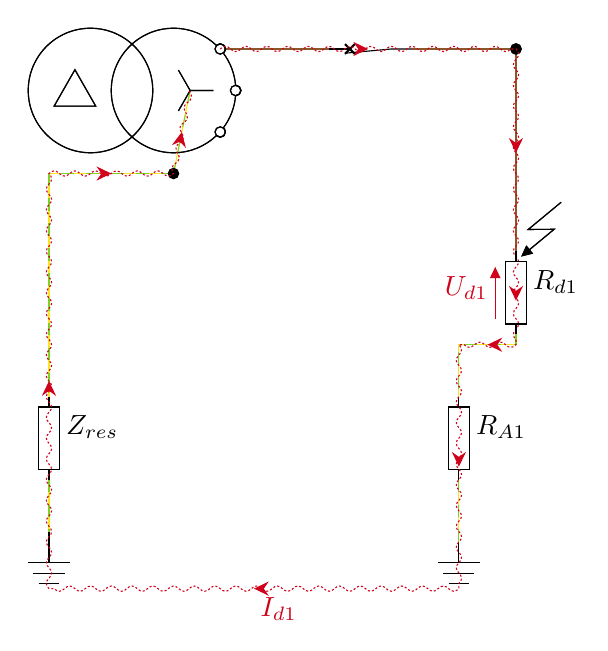
\begin{tikzpicture}[x=0.75pt,y=0.75pt,yscale=-1,xscale=1]
%uncomment if require: \path (0,313); %set diagram left start at 0, and has height of 313

%Straight Lines [id:da40140774002563195] 
\draw [color={rgb, 255:red, 248; green, 231; blue, 28 }  ,draw opacity=1 ]   (87.5,75) -- (27.5,75) -- (27.5,182.5) ;
%Straight Lines [id:da7768656062968136] 
\draw [color={rgb, 255:red, 248; green, 231; blue, 28 }  ,draw opacity=1 ]   (95.5,35) -- (87.5,75) ;
%Straight Lines [id:da0702550211386399] 
\draw [color={rgb, 255:red, 126; green, 211; blue, 33 }  ,draw opacity=1 ] [dash pattern={on 4.5pt off 4.5pt}]  (95.5,35) -- (87.5,75) ;
%Shape: Path Data [id:dp6564394705196642] 
\draw   (112.5,55) .. controls (112.5,56.38) and (111.38,57.5) .. (110,57.5) .. controls (109.29,57.5) and (108.65,57.2) .. (108.19,56.72) .. controls (102.81,61.85) and (95.52,65) .. (87.5,65) .. controls (70.93,65) and (57.5,51.57) .. (57.5,35) .. controls (57.5,18.43) and (70.93,5) .. (87.5,5) .. controls (95.52,5) and (102.81,8.15) .. (108.19,13.28) .. controls (108.65,12.8) and (109.29,12.5) .. (110,12.5) .. controls (111.38,12.5) and (112.5,13.62) .. (112.5,15) .. controls (112.5,15.82) and (112.11,16.54) .. (111.5,17) .. controls (114.8,21.39) and (116.92,26.71) .. (117.4,32.5) .. controls (117.43,32.5) and (117.47,32.5) .. (117.5,32.5) .. controls (118.88,32.5) and (120,33.62) .. (120,35) .. controls (120,36.38) and (118.88,37.5) .. (117.5,37.5) .. controls (117.47,37.5) and (117.43,37.5) .. (117.4,37.5) .. controls (116.92,43.29) and (114.8,48.61) .. (111.5,53) .. controls (112.11,53.46) and (112.5,54.18) .. (112.5,55) -- cycle ;
%Shape: Circle [id:dp6837865910950578] 
\draw   (17.5,35) .. controls (17.5,18.43) and (30.93,5) .. (47.5,5) .. controls (64.07,5) and (77.5,18.43) .. (77.5,35) .. controls (77.5,51.57) and (64.07,65) .. (47.5,65) .. controls (30.93,65) and (17.5,51.57) .. (17.5,35) -- cycle ;
%Shape: Triangle [id:dp4328019700995849] 
\draw   (40,25) -- (30,42.5) -- (50,42.5) -- cycle ;
%Shape: Star [id:dp9996543744584487] 
\draw   (106.75,35) -- (95.5,35) -- (89.88,44.81) -- (95.5,35) -- (89.88,25.19) -- (95.5,35) -- cycle ;
%Shape: Circle [id:dp4765432529475536] 
\draw   (107.5,15) .. controls (107.5,13.62) and (108.62,12.5) .. (110,12.5) .. controls (111.38,12.5) and (112.5,13.62) .. (112.5,15) .. controls (112.5,16.38) and (111.38,17.5) .. (110,17.5) .. controls (108.62,17.5) and (107.5,16.38) .. (107.5,15) -- cycle ;
%Shape: Circle [id:dp7950957606894842] 
\draw   (114.9,35) .. controls (114.9,33.62) and (116.02,32.5) .. (117.4,32.5) .. controls (118.78,32.5) and (119.9,33.62) .. (119.9,35) .. controls (119.9,36.38) and (118.78,37.5) .. (117.4,37.5) .. controls (116.02,37.5) and (114.9,36.38) .. (114.9,35) -- cycle ;
%Shape: Circle [id:dp47024921818209997] 
\draw   (107.5,55) .. controls (107.5,53.62) and (108.62,52.5) .. (110,52.5) .. controls (111.38,52.5) and (112.5,53.62) .. (112.5,55) .. controls (112.5,56.38) and (111.38,57.5) .. (110,57.5) .. controls (108.62,57.5) and (107.5,56.38) .. (107.5,55) -- cycle ;

%Straight Lines [id:da21818556641513764] 
\draw [color={rgb, 255:red, 139; green, 87; blue, 42 }  ,draw opacity=1 ]   (252.5,112.5) -- (252.5,17.5) ;
%Straight Lines [id:da8686907197740312] 
\draw [color={rgb, 255:red, 248; green, 231; blue, 28 }  ,draw opacity=1 ]   (225,222.5) -- (225,247.5) ;
%Straight Lines [id:da4369452606894554] 
\draw    (225,247.5) -- (225,262.5) ;
%Straight Lines [id:da41347797921121543] 
\draw    (215,262.5) -- (235,262.5) ;
%Straight Lines [id:da39005220989882616] 
\draw    (217.5,267.5) -- (232.5,267.5) ;
%Straight Lines [id:da04530437508662333] 
\draw    (220,272.5) -- (230,272.5) ;

%Straight Lines [id:da758878567860916] 
\draw [color={rgb, 255:red, 126; green, 211; blue, 33 }  ,draw opacity=1 ] [dash pattern={on 4.5pt off 4.5pt}]  (225,222.5) -- (225,247.5) ;
%Straight Lines [id:da7282446695874194] 
\draw    (225,217.5) -- (225,222.5) ;
%Shape: Rectangle [id:dp5377265306575283] 
\draw   (230,187.5) -- (230,217.5) -- (220,217.5) -- (220,187.5) -- cycle ;
%Straight Lines [id:da6172743564243196] 
\draw    (225,182.5) -- (225,187.5) ;

%Shape: Circle [id:dp9518184334454515] 
\draw  [fill={rgb, 255:red, 0; green, 0; blue, 0 }  ,fill opacity=1 ] (250,15) .. controls (250,13.62) and (251.12,12.5) .. (252.5,12.5) .. controls (253.88,12.5) and (255,13.62) .. (255,15) .. controls (255,16.38) and (253.88,17.5) .. (252.5,17.5) .. controls (251.12,17.5) and (250,16.38) .. (250,15) -- cycle ;
%Straight Lines [id:da698344453228456] 
\draw [color={rgb, 255:red, 139; green, 87; blue, 42 }  ,draw opacity=1 ]   (112.5,15) -- (162.5,15) ;
%Straight Lines [id:da3888199822065723] 
\draw [color={rgb, 255:red, 126; green, 211; blue, 33 }  ,draw opacity=1 ] [dash pattern={on 4.5pt off 4.5pt}]  (87.5,75) -- (27.5,75) -- (27.5,182.5) ;
%Straight Lines [id:da9929118367256647] 
\draw    (27.5,217.5) -- (27.5,222.5) ;
%Shape: Rectangle [id:dp5522927597315069] 
\draw   (32.5,187.5) -- (32.5,217.5) -- (22.5,217.5) -- (22.5,187.5) -- cycle ;
%Straight Lines [id:da51565112690186] 
\draw    (27.5,182.5) -- (27.5,187.5) ;

%Straight Lines [id:da20200008374801148] 
\draw [color={rgb, 255:red, 248; green, 231; blue, 28 }  ,draw opacity=1 ]   (27.5,222.5) -- (27.5,247.5) ;
%Straight Lines [id:da246860902568655] 
\draw [color={rgb, 255:red, 126; green, 211; blue, 33 }  ,draw opacity=1 ] [dash pattern={on 4.5pt off 4.5pt}]  (27.5,222.5) -- (27.5,247.5) ;
%Straight Lines [id:da8847595831515674] 
\draw    (27.5,247.5) -- (27.5,262.5) ;
%Straight Lines [id:da388525152974063] 
\draw    (17.5,262.5) -- (37.5,262.5) ;
%Straight Lines [id:da5307482611563814] 
\draw    (20,267.5) -- (35,267.5) ;
%Straight Lines [id:da879280977386573] 
\draw    (22.5,272.5) -- (32.5,272.5) ;

%Shape: Circle [id:dp23726887554171172] 
\draw  [fill={rgb, 255:red, 0; green, 0; blue, 0 }  ,fill opacity=1 ] (85,75) .. controls (85,73.62) and (86.12,72.5) .. (87.5,72.5) .. controls (88.88,72.5) and (90,73.62) .. (90,75) .. controls (90,76.38) and (88.88,77.5) .. (87.5,77.5) .. controls (86.12,77.5) and (85,76.38) .. (85,75) -- cycle ;
%Shape: Boxed Line [id:dp0646171917121674] 
\draw    (274.27,88.83) -- (258.39,101.97) -- (270.89,101.86) -- (257.31,113.09) ;
\draw [shift={(255,115)}, rotate = 320.40999999999997] [fill={rgb, 255:red, 0; green, 0; blue, 0 }  ][line width=0.08]  [draw opacity=0] (5.36,-2.57) -- (0,0) -- (5.36,2.57) -- cycle    ;
%Straight Lines [id:da0893199801246688] 
\draw    (170.5,17) -- (192.5,15) -- (202.5,15) ;
%Straight Lines [id:da4465712907894863] 
\draw    (172.5,15) -- (162.5,15) ;
\draw [shift={(172.5,15)}, rotate = 225] [color={rgb, 255:red, 0; green, 0; blue, 0 }  ][line width=0.75]    (-3.35,0) -- (3.35,0)(0,3.35) -- (0,-3.35)   ;

%Straight Lines [id:da6575503286927553] 
\draw [color={rgb, 255:red, 248; green, 231; blue, 28 }  ,draw opacity=1 ]   (252.5,152.5) -- (252.5,157.5) -- (225,157.5) -- (225,182.5) ;
%Straight Lines [id:da4804418012067295] 
\draw [color={rgb, 255:red, 139; green, 87; blue, 42 }  ,draw opacity=1 ]   (112.5,15) -- (162.5,15) ;
%Straight Lines [id:da7896587451085693] 
\draw [color={rgb, 255:red, 139; green, 87; blue, 42 }  ,draw opacity=1 ]   (202.5,15) -- (252.5,15) ;
%Shape: Path Data [id:dp195065302202169] 
\draw   (112.5,55) .. controls (112.5,56.38) and (111.38,57.5) .. (110,57.5) .. controls (109.29,57.5) and (108.65,57.2) .. (108.19,56.72) .. controls (102.81,61.85) and (95.52,65) .. (87.5,65) .. controls (70.93,65) and (57.5,51.57) .. (57.5,35) .. controls (57.5,18.43) and (70.93,5) .. (87.5,5) .. controls (95.52,5) and (102.81,8.15) .. (108.19,13.28) .. controls (108.65,12.8) and (109.29,12.5) .. (110,12.5) .. controls (111.38,12.5) and (112.5,13.62) .. (112.5,15) .. controls (112.5,15.82) and (112.11,16.54) .. (111.5,17) .. controls (114.8,21.39) and (116.92,26.71) .. (117.4,32.5) .. controls (117.43,32.5) and (117.47,32.5) .. (117.5,32.5) .. controls (118.88,32.5) and (120,33.62) .. (120,35) .. controls (120,36.38) and (118.88,37.5) .. (117.5,37.5) .. controls (117.47,37.5) and (117.43,37.5) .. (117.4,37.5) .. controls (116.92,43.29) and (114.8,48.61) .. (111.5,53) .. controls (112.11,53.46) and (112.5,54.18) .. (112.5,55) -- cycle ;
%Shape: Circle [id:dp10449815547230978] 
\draw   (17.5,35) .. controls (17.5,18.43) and (30.93,5) .. (47.5,5) .. controls (64.07,5) and (77.5,18.43) .. (77.5,35) .. controls (77.5,51.57) and (64.07,65) .. (47.5,65) .. controls (30.93,65) and (17.5,51.57) .. (17.5,35) -- cycle ;
%Shape: Triangle [id:dp13602835689186588] 
\draw   (40,25) -- (30,42.5) -- (50,42.5) -- cycle ;
%Shape: Star [id:dp5246434088790826] 
\draw   (106.75,35) -- (95.5,35) -- (89.88,44.81) -- (95.5,35) -- (89.88,25.19) -- (95.5,35) -- cycle ;
%Shape: Circle [id:dp3622486105745091] 
\draw   (107.5,15) .. controls (107.5,13.62) and (108.62,12.5) .. (110,12.5) .. controls (111.38,12.5) and (112.5,13.62) .. (112.5,15) .. controls (112.5,16.38) and (111.38,17.5) .. (110,17.5) .. controls (108.62,17.5) and (107.5,16.38) .. (107.5,15) -- cycle ;
%Shape: Circle [id:dp7116693252528491] 
\draw   (114.9,35) .. controls (114.9,33.62) and (116.02,32.5) .. (117.4,32.5) .. controls (118.78,32.5) and (119.9,33.62) .. (119.9,35) .. controls (119.9,36.38) and (118.78,37.5) .. (117.4,37.5) .. controls (116.02,37.5) and (114.9,36.38) .. (114.9,35) -- cycle ;
%Shape: Circle [id:dp18972999107641209] 
\draw   (107.5,55) .. controls (107.5,53.62) and (108.62,52.5) .. (110,52.5) .. controls (111.38,52.5) and (112.5,53.62) .. (112.5,55) .. controls (112.5,56.38) and (111.38,57.5) .. (110,57.5) .. controls (108.62,57.5) and (107.5,56.38) .. (107.5,55) -- cycle ;

%Straight Lines [id:da014549812099070136] 
\draw [color={rgb, 255:red, 139; green, 87; blue, 42 }  ,draw opacity=1 ]   (252.5,112.5) -- (252.5,17.5) ;
%Straight Lines [id:da26084750256284417] 
\draw [color={rgb, 255:red, 126; green, 211; blue, 33 }  ,draw opacity=1 ] [dash pattern={on 4.5pt off 4.5pt}]  (252.5,152.5) -- (252.5,157.5) -- (225,157.5) -- (225,182.5) ;
%Straight Lines [id:da3030992302203893] 
\draw [color={rgb, 255:red, 248; green, 231; blue, 28 }  ,draw opacity=1 ]   (225,222.5) -- (225,252.5) ;
%Straight Lines [id:da15920917753755837] 
\draw [color={rgb, 255:red, 126; green, 211; blue, 33 }  ,draw opacity=1 ] [dash pattern={on 4.5pt off 4.5pt}]  (225,222.5) -- (225,252.5) ;
%Shape: Circle [id:dp17133751283477605] 
\draw  [fill={rgb, 255:red, 0; green, 0; blue, 0 }  ,fill opacity=1 ] (250,15) .. controls (250,13.62) and (251.12,12.5) .. (252.5,12.5) .. controls (253.88,12.5) and (255,13.62) .. (255,15) .. controls (255,16.38) and (253.88,17.5) .. (252.5,17.5) .. controls (251.12,17.5) and (250,16.38) .. (250,15) -- cycle ;
%Shape: Boxed Line [id:dp8068084114642486] 
\draw    (274.27,88.83) -- (258.39,101.97) -- (270.89,101.86) -- (257.31,113.09) ;
\draw [shift={(255,115)}, rotate = 320.40999999999997] [fill={rgb, 255:red, 0; green, 0; blue, 0 }  ][line width=0.08]  [draw opacity=0] (5.36,-2.57) -- (0,0) -- (5.36,2.57) -- cycle    ;
%Straight Lines [id:da21551575051470273] 
\draw [color={rgb, 255:red, 208; green, 2; blue, 27 }  ,draw opacity=1 ] [dash pattern={on 0.75pt off 0.75pt}]  (110,15) .. controls (111.67,13.33) and (113.33,13.33) .. (115,15) .. controls (116.67,16.67) and (118.33,16.67) .. (120,15) .. controls (121.67,13.33) and (123.33,13.33) .. (125,15) .. controls (126.67,16.67) and (128.33,16.67) .. (130,15) .. controls (131.67,13.33) and (133.33,13.33) .. (135,15) .. controls (136.67,16.67) and (138.33,16.67) .. (140,15) .. controls (141.67,13.33) and (143.33,13.33) .. (145,15) .. controls (146.67,16.67) and (148.33,16.67) .. (150,15) .. controls (151.67,13.33) and (153.33,13.33) .. (155,15) .. controls (156.67,16.67) and (158.33,16.67) .. (160,15) .. controls (161.67,13.33) and (163.33,13.33) .. (165,15) .. controls (166.67,16.67) and (168.33,16.67) .. (170,15) .. controls (171.67,13.33) and (173.33,13.33) .. (175,15) .. controls (176.67,16.67) and (178.33,16.67) .. (180,15) .. controls (181.67,13.33) and (183.33,13.33) .. (185,15) .. controls (186.67,16.67) and (188.33,16.67) .. (190,15) .. controls (191.67,13.33) and (193.33,13.33) .. (195,15) .. controls (196.67,16.67) and (198.33,16.67) .. (200,15) .. controls (201.67,13.33) and (203.33,13.33) .. (205,15) .. controls (206.67,16.67) and (208.33,16.67) .. (210,15) .. controls (211.67,13.33) and (213.33,13.33) .. (215,15) .. controls (216.67,16.67) and (218.33,16.67) .. (220,15) .. controls (221.67,13.33) and (223.33,13.33) .. (225,15) .. controls (226.67,16.67) and (228.33,16.67) .. (230,15) .. controls (231.67,13.33) and (233.33,13.33) .. (235,15) .. controls (236.67,16.67) and (238.33,16.67) .. (240,15) .. controls (241.67,13.33) and (243.33,13.33) .. (245,15) .. controls (246.67,16.67) and (248.33,16.67) .. (250,15) -- (252.5,15) -- (252.5,15) .. controls (254.17,16.67) and (254.17,18.33) .. (252.5,20) .. controls (250.83,21.67) and (250.83,23.33) .. (252.5,25) .. controls (254.17,26.67) and (254.17,28.33) .. (252.5,30) .. controls (250.83,31.67) and (250.83,33.33) .. (252.5,35) .. controls (254.17,36.67) and (254.17,38.33) .. (252.5,40) .. controls (250.83,41.67) and (250.83,43.33) .. (252.5,45) .. controls (254.17,46.67) and (254.17,48.33) .. (252.5,50) .. controls (250.83,51.67) and (250.83,53.33) .. (252.5,55) .. controls (254.17,56.67) and (254.17,58.33) .. (252.5,60) .. controls (250.83,61.67) and (250.83,63.33) .. (252.5,65) .. controls (254.17,66.67) and (254.17,68.33) .. (252.5,70) .. controls (250.83,71.67) and (250.83,73.33) .. (252.5,75) .. controls (254.17,76.67) and (254.17,78.33) .. (252.5,80) .. controls (250.83,81.67) and (250.83,83.33) .. (252.5,85) .. controls (254.17,86.67) and (254.17,88.33) .. (252.5,90) .. controls (250.83,91.67) and (250.83,93.33) .. (252.5,95) .. controls (254.17,96.67) and (254.17,98.33) .. (252.5,100) .. controls (250.83,101.67) and (250.83,103.33) .. (252.5,105) .. controls (254.17,106.67) and (254.17,108.33) .. (252.5,110) .. controls (250.83,111.67) and (250.83,113.33) .. (252.5,115) -- (252.5,115) .. controls (254.17,116.67) and (254.17,118.33) .. (252.5,120) .. controls (250.83,121.67) and (250.83,123.33) .. (252.5,125) .. controls (254.17,126.67) and (254.17,128.33) .. (252.5,130) .. controls (250.83,131.67) and (250.83,133.33) .. (252.5,135) .. controls (254.17,136.67) and (254.17,138.33) .. (252.5,140) .. controls (250.83,141.67) and (250.83,143.33) .. (252.5,145) .. controls (254.17,146.67) and (254.17,148.33) .. (252.5,150) .. controls (250.83,151.67) and (250.83,153.33) .. (252.5,155) -- (252.5,157.5) -- (252.5,157.5) .. controls (250.83,159.17) and (249.17,159.17) .. (247.5,157.5) .. controls (245.83,155.83) and (244.17,155.83) .. (242.5,157.5) .. controls (240.83,159.17) and (239.17,159.17) .. (237.5,157.5) .. controls (235.83,155.83) and (234.17,155.83) .. (232.5,157.5) .. controls (230.83,159.17) and (229.17,159.17) .. (227.5,157.5) -- (225,157.5) -- (225,157.5) .. controls (226.67,159.17) and (226.67,160.83) .. (225,162.5) .. controls (223.33,164.17) and (223.33,165.83) .. (225,167.5) .. controls (226.67,169.17) and (226.67,170.83) .. (225,172.5) .. controls (223.33,174.17) and (223.33,175.83) .. (225,177.5) .. controls (226.67,179.17) and (226.67,180.83) .. (225,182.5) .. controls (223.33,184.17) and (223.33,185.83) .. (225,187.5) .. controls (226.67,189.17) and (226.67,190.83) .. (225,192.5) .. controls (223.33,194.17) and (223.33,195.83) .. (225,197.5) .. controls (226.67,199.17) and (226.67,200.83) .. (225,202.5) .. controls (223.33,204.17) and (223.33,205.83) .. (225,207.5) .. controls (226.67,209.17) and (226.67,210.83) .. (225,212.5) .. controls (223.33,214.17) and (223.33,215.83) .. (225,217.5) .. controls (226.67,219.17) and (226.67,220.83) .. (225,222.5) .. controls (223.33,224.17) and (223.33,225.83) .. (225,227.5) .. controls (226.67,229.17) and (226.67,230.83) .. (225,232.5) .. controls (223.33,234.17) and (223.33,235.83) .. (225,237.5) .. controls (226.67,239.17) and (226.67,240.83) .. (225,242.5) .. controls (223.33,244.17) and (223.33,245.83) .. (225,247.5) .. controls (226.67,249.17) and (226.67,250.83) .. (225,252.5) .. controls (223.33,254.17) and (223.33,255.83) .. (225,257.5) .. controls (226.67,259.17) and (226.67,260.83) .. (225,262.5) .. controls (223.33,264.17) and (223.33,265.83) .. (225,267.5) .. controls (226.67,269.17) and (226.67,270.83) .. (225,272.5) -- (225,275) -- (225,275) .. controls (223.33,276.67) and (221.67,276.67) .. (220,275) .. controls (218.33,273.33) and (216.67,273.33) .. (215,275) .. controls (213.33,276.67) and (211.67,276.67) .. (210,275) .. controls (208.33,273.33) and (206.67,273.33) .. (205,275) .. controls (203.33,276.67) and (201.67,276.67) .. (200,275) .. controls (198.33,273.33) and (196.67,273.33) .. (195,275) .. controls (193.33,276.67) and (191.67,276.67) .. (190,275) .. controls (188.33,273.33) and (186.67,273.33) .. (185,275) .. controls (183.33,276.67) and (181.67,276.67) .. (180,275) .. controls (178.33,273.33) and (176.67,273.33) .. (175,275) .. controls (173.33,276.67) and (171.67,276.67) .. (170,275) .. controls (168.33,273.33) and (166.67,273.33) .. (165,275) .. controls (163.33,276.67) and (161.67,276.67) .. (160,275) .. controls (158.33,273.33) and (156.67,273.33) .. (155,275) .. controls (153.33,276.67) and (151.67,276.67) .. (150,275) .. controls (148.33,273.33) and (146.67,273.33) .. (145,275) .. controls (143.33,276.67) and (141.67,276.67) .. (140,275) .. controls (138.33,273.33) and (136.67,273.33) .. (135,275) .. controls (133.33,276.67) and (131.67,276.67) .. (130,275) .. controls (128.33,273.33) and (126.67,273.33) .. (125,275) .. controls (123.33,276.67) and (121.67,276.67) .. (120,275) .. controls (118.33,273.33) and (116.67,273.33) .. (115,275) .. controls (113.33,276.67) and (111.67,276.67) .. (110,275) .. controls (108.33,273.33) and (106.67,273.33) .. (105,275) .. controls (103.33,276.67) and (101.67,276.67) .. (100,275) .. controls (98.33,273.33) and (96.67,273.33) .. (95,275) .. controls (93.33,276.67) and (91.67,276.67) .. (90,275) .. controls (88.33,273.33) and (86.67,273.33) .. (85,275) .. controls (83.33,276.67) and (81.67,276.67) .. (80,275) .. controls (78.33,273.33) and (76.67,273.33) .. (75,275) .. controls (73.33,276.67) and (71.67,276.67) .. (70,275) .. controls (68.33,273.33) and (66.67,273.33) .. (65,275) .. controls (63.33,276.67) and (61.67,276.67) .. (60,275) .. controls (58.33,273.33) and (56.67,273.33) .. (55,275) .. controls (53.33,276.67) and (51.67,276.67) .. (50,275) .. controls (48.33,273.33) and (46.67,273.33) .. (45,275) .. controls (43.33,276.67) and (41.67,276.67) .. (40,275) .. controls (38.33,273.33) and (36.67,273.33) .. (35,275) .. controls (33.33,276.67) and (31.67,276.67) .. (30,275) -- (27.5,275) -- (27.5,275) .. controls (25.83,273.33) and (25.83,271.67) .. (27.5,270) .. controls (29.17,268.33) and (29.17,266.67) .. (27.5,265) .. controls (25.83,263.33) and (25.83,261.67) .. (27.5,260) .. controls (29.17,258.33) and (29.17,256.67) .. (27.5,255) .. controls (25.83,253.33) and (25.83,251.67) .. (27.5,250) .. controls (29.17,248.33) and (29.17,246.67) .. (27.5,245) .. controls (25.83,243.33) and (25.83,241.67) .. (27.5,240) .. controls (29.17,238.33) and (29.17,236.67) .. (27.5,235) .. controls (25.83,233.33) and (25.83,231.67) .. (27.5,230) .. controls (29.17,228.33) and (29.17,226.67) .. (27.5,225) .. controls (25.83,223.33) and (25.83,221.67) .. (27.5,220) .. controls (29.17,218.33) and (29.17,216.67) .. (27.5,215) .. controls (25.83,213.33) and (25.83,211.67) .. (27.5,210) .. controls (29.17,208.33) and (29.17,206.67) .. (27.5,205) .. controls (25.83,203.33) and (25.83,201.67) .. (27.5,200) .. controls (29.17,198.33) and (29.17,196.67) .. (27.5,195) .. controls (25.83,193.33) and (25.83,191.67) .. (27.5,190) .. controls (29.17,188.33) and (29.17,186.67) .. (27.5,185) .. controls (25.83,183.33) and (25.83,181.67) .. (27.5,180) .. controls (29.17,178.33) and (29.17,176.67) .. (27.5,175) .. controls (25.83,173.33) and (25.83,171.67) .. (27.5,170) .. controls (29.17,168.33) and (29.17,166.67) .. (27.5,165) .. controls (25.83,163.33) and (25.83,161.67) .. (27.5,160) .. controls (29.17,158.33) and (29.17,156.67) .. (27.5,155) .. controls (25.83,153.33) and (25.83,151.67) .. (27.5,150) .. controls (29.17,148.33) and (29.17,146.67) .. (27.5,145) .. controls (25.83,143.33) and (25.83,141.67) .. (27.5,140) .. controls (29.17,138.33) and (29.17,136.67) .. (27.5,135) .. controls (25.83,133.33) and (25.83,131.67) .. (27.5,130) .. controls (29.17,128.33) and (29.17,126.67) .. (27.5,125) .. controls (25.83,123.33) and (25.83,121.67) .. (27.5,120) .. controls (29.17,118.33) and (29.17,116.67) .. (27.5,115) .. controls (25.83,113.33) and (25.83,111.67) .. (27.5,110) .. controls (29.17,108.33) and (29.17,106.67) .. (27.5,105) .. controls (25.83,103.33) and (25.83,101.67) .. (27.5,100) .. controls (29.17,98.33) and (29.17,96.67) .. (27.5,95) .. controls (25.83,93.33) and (25.83,91.67) .. (27.5,90) .. controls (29.17,88.33) and (29.17,86.67) .. (27.5,85) .. controls (25.83,83.33) and (25.83,81.67) .. (27.5,80) .. controls (29.17,78.33) and (29.17,76.67) .. (27.5,75) -- (27.5,75) .. controls (29.17,73.33) and (30.83,73.33) .. (32.5,75) .. controls (34.17,76.67) and (35.83,76.67) .. (37.5,75) .. controls (39.17,73.33) and (40.83,73.33) .. (42.5,75) .. controls (44.17,76.67) and (45.83,76.67) .. (47.5,75) .. controls (49.17,73.33) and (50.83,73.33) .. (52.5,75) .. controls (54.17,76.67) and (55.83,76.67) .. (57.5,75) .. controls (59.17,73.33) and (60.83,73.33) .. (62.5,75) .. controls (64.17,76.67) and (65.83,76.67) .. (67.5,75) .. controls (69.17,73.33) and (70.83,73.33) .. (72.5,75) .. controls (74.17,76.67) and (75.83,76.67) .. (77.5,75) .. controls (79.17,73.33) and (80.83,73.33) .. (82.5,75) .. controls (84.17,76.67) and (85.83,76.67) .. (87.5,75) -- (87.5,75) .. controls (86.19,73.04) and (86.52,71.41) .. (88.48,70.1) .. controls (90.44,68.79) and (90.77,67.15) .. (89.46,65.19) .. controls (88.15,63.23) and (88.48,61.6) .. (90.44,60.29) .. controls (92.4,58.98) and (92.73,57.35) .. (91.42,55.39) .. controls (90.11,53.43) and (90.44,51.8) .. (92.4,50.49) .. controls (94.36,49.18) and (94.69,47.54) .. (93.38,45.58) .. controls (92.07,43.62) and (92.4,41.99) .. (94.36,40.68) .. controls (96.32,39.37) and (96.65,37.74) .. (95.34,35.78) -- (95.5,35) -- (95.5,35) ;
\draw [shift={(181.25,15)}, rotate = 180] [fill={rgb, 255:red, 208; green, 2; blue, 27 }  ,fill opacity=1 ][line width=0.08]  [draw opacity=0] (7.14,-3.43) -- (0,0) -- (7.14,3.43) -- (4.74,0) -- cycle    ;
\draw [shift={(252.5,65)}, rotate = 270] [fill={rgb, 255:red, 208; green, 2; blue, 27 }  ,fill opacity=1 ][line width=0.08]  [draw opacity=0] (7.14,-3.43) -- (0,0) -- (7.14,3.43) -- (4.74,0) -- cycle    ;
\draw [shift={(252.5,136.25)}, rotate = 270] [fill={rgb, 255:red, 208; green, 2; blue, 27 }  ,fill opacity=1 ][line width=0.08]  [draw opacity=0] (7.14,-3.43) -- (0,0) -- (7.14,3.43) -- (4.74,0) -- cycle    ;
\draw [shift={(238.75,157.5)}, rotate = 360] [fill={rgb, 255:red, 208; green, 2; blue, 27 }  ,fill opacity=1 ][line width=0.08]  [draw opacity=0] (7.14,-3.43) -- (0,0) -- (7.14,3.43) -- (4.74,0) -- cycle    ;
\draw [shift={(225,216.25)}, rotate = 270] [fill={rgb, 255:red, 208; green, 2; blue, 27 }  ,fill opacity=1 ][line width=0.08]  [draw opacity=0] (7.14,-3.43) -- (0,0) -- (7.14,3.43) -- (4.74,0) -- cycle    ;
\draw [shift={(126.25,275)}, rotate = 360] [fill={rgb, 255:red, 208; green, 2; blue, 27 }  ,fill opacity=1 ][line width=0.08]  [draw opacity=0] (7.14,-3.43) -- (0,0) -- (7.14,3.43) -- (4.74,0) -- cycle    ;
\draw [shift={(27.5,175)}, rotate = 450] [fill={rgb, 255:red, 208; green, 2; blue, 27 }  ,fill opacity=1 ][line width=0.08]  [draw opacity=0] (7.14,-3.43) -- (0,0) -- (7.14,3.43) -- (4.74,0) -- cycle    ;
\draw [shift={(57.5,75)}, rotate = 180] [fill={rgb, 255:red, 208; green, 2; blue, 27 }  ,fill opacity=1 ][line width=0.08]  [draw opacity=0] (7.14,-3.43) -- (0,0) -- (7.14,3.43) -- (4.74,0) -- cycle    ;
\draw [shift={(91.5,55)}, rotate = 461.31] [fill={rgb, 255:red, 208; green, 2; blue, 27 }  ,fill opacity=1 ][line width=0.08]  [draw opacity=0] (7.14,-3.43) -- (0,0) -- (7.14,3.43) -- (4.74,0) -- cycle    ;
%Straight Lines [id:da5878987587379367] 
\draw    (252.5,147.5) -- (252.5,152.5) ;
%Shape: Rectangle [id:dp5233395725568003] 
\draw   (257.5,117.5) -- (257.5,147.5) -- (247.5,147.5) -- (247.5,117.5) -- cycle ;
%Straight Lines [id:da6884797067797518] 
\draw    (252.5,112.5) -- (252.5,117.5) ;

%Straight Lines [id:da07071854927031873] 
\draw [color={rgb, 255:red, 208; green, 2; blue, 27 }  ,draw opacity=1 ]   (242.5,123) -- (242.5,145) ;
\draw [shift={(242.5,120)}, rotate = 90] [fill={rgb, 255:red, 208; green, 2; blue, 27 }  ,fill opacity=1 ][line width=0.08]  [draw opacity=0] (5.36,-2.57) -- (0,0) -- (5.36,2.57) -- cycle    ;

% Text Node
\draw (232,190.5) node [anchor=north west][inner sep=0.75pt]   [align=left] {$R_{A1}$};
% Text Node
\draw (34.5,190.5) node [anchor=north west][inner sep=0.75pt]   [align=left] {$Z_{res}$};
% Text Node
\draw (128.25,278) node [anchor=north west][inner sep=0.75pt]  [color={rgb, 255:red, 208; green, 2; blue, 27 }  ,opacity=1 ] [align=left] {$I_{d1}$};
% Text Node
\draw (217,123.5) node [anchor=north west][inner sep=0.75pt]  [color={rgb, 255:red, 208; green, 2; blue, 27 }  ,opacity=1 ] [align=left] {$U_{d1}$};
% Text Node
\draw (259.5,120.5) node [anchor=north west][inner sep=0.75pt]   [align=left] {$R_{d1}$};


\end{tikzpicture}
\end{figure}

%\end{document}


L'intensité de courant $I_d1$ vaut alors :
\begin{formule}{Courant du premier défaut $I_d1$ en schéma Isolé-Individuel}{}
\begin{align*}
		I_d &= \frac{U_{0}}{Z_{res}+R_{A1}+R_{d1}}
\end{align*}

\begin{textvariables}
U_{0}						& tension nominale simple						& volt			& \volt					& 	Différence de potentiel entre les masses métalliques et la terre 	\\
Z_{res}						& impédance											& ohm			& \ohm					& 	Impédance de fuite $Z_res$ du réseau électrique 	\\
R_{A1}						& résistance											& ohm			& \ohm					& 	Résistance de la prise de terre de l'appareil 1 	\\
R_{d1}						& résistance											& ohm			& \ohm					& 	Résistance de défaut 	d'isolement de l'appareil 1\\
\end{textvariables}
\end{formule}

Le courant de défaut $I_{d1}$ fera alors apparaître une \emph{tension de défaut} $U_{d1}$ entre la masse métallique de l'appareil 1 et la terre. Cette tension, limitée par l'impédance de fuite, sera très largement inférieure à  $U_L$ et ne sera donc pas dangereuse. La situation sera similaire avec un schéma Impédant-Individuel $Z_N$, ou l'impédance de limitation limitera également le courant de défaut :

\begin{formule}{Tension de défaut $U_{d1}$ en schéma Isolé-Individuel}{}
\begin{align*}
		U_{d1} &= R_{A1} \times I_{d1} \\
			   &\ll	 U_L
\end{align*}

\begin{textvariables}
R_{A1}						& résistance											& ohm			& \ohm					& 	Résistance de la prise de terre de l'appareil 1 	\\
I_{d1}							& intensité							& ampère		& \ampere				& 	Courant de défaut de l'appareil 1\\
U_{L}						& tension							& volt			& \volt					& 	Tension de sécurité du local avec :
\begin{description}[nosep, leftmargin=*]
\item[Local sec :] $U_{L}=\SI{50}{\volt}$
\item[Local humide :] $U_{L}=\SI{25}{\volt}$
\end{description} \\
\end{textvariables}
\end{formule}

Le fonctionnement d'un schéma IT sera également identique au premier défaut, que les masses soient interconnectées ou individuellement raccordées à la terre.

\begin{exemple}{Tension de défaut $U_{d1}$ en schéma Isolé-Individuel au premier défaut}{}
Si on considère que le transformateur est un transformateur $\SI{20}{\kilo\volt}/\SI{400}{\volt}$, que $Z_{res}=\SI{3500}{\ohm}$, $R_{A1}=\SI{40}{\ohm}$ et que $R_d = \SI{2}{\ohm}$, on peut déduire que le courant de défaut $I_d$ vaut :
\begin{align*}
		I_{d1} &= \frac{U_{0}}{Z_{res}+R_{A1}+R_{d1}} \\
				&=\frac{400}{3500+40+2} \\
				&= \SI{64,9}{\milli\ampere} \\
\end{align*}
Si une personne touche à la masse du récepteur 1, elle sera soumise à une tension de défaut $U_{d1}$ :
\begin{align*}
		U_{d1} &= R_{A1} \times I_{d1} \\
				&=40 \times 0,0649 \\
				&= \SI{2,6}{\volt}
\end{align*}
\end{exemple}

Lors de l'apparition d'un deuxième défaut d'isolement sur un autre conducteur actif, un courant de défaut $I_{d2}$ va apparaitre. Celui-ci va s'apparenter à un court-circuit et de ce fait, $I_{d1}$ sera négligé. \\
Dans les calculs, il faut encore tenir compte de la \emph{résistance de défaut} $R_d$ qui prend en compte la nature du défaut d'isolement (franc ou non-franc) et les résistances des carcasses métalliques des appareils 1 et 2.\\

\begin{figure}[H]
\caption{Installation Isolé-Individuelle}
\begin{subfigure}[t]{0.49\linewidth}
%--------------------------------------
%ELECTROTECHNIQUE - SCHEMA DE LIAISON A LA TERRE
%--------------------------------------

%utiliser les environnement \begin{comment} \end{comment} pour mettre en commentaire le préambule une fois la programmation appelée dans le document maître (!ne pas oublier de mettre en commentaire \end{document}!)

\begin{comment}

\documentclass[a4paper, 11pt, twoside, fleqn]{memoir}

\usepackage{AOCDTF}

\marqueurchapitre
\decoupagechapitre{1} %juste pour éviter les erreurs lors de la compilation des sous-programmations (passera en commentaire)

%lien d'édition des figures Tikz sur le site mathcha.io (rajouter le lien d'une modification effectuée sur la figure tikz avec le nom du modificateur car il n'y a qu'un lien par compte)

%lien mathcha Bruno Douchy : https://www.mathcha.io/editor/DXXG1FgjiNJCe0yo2ZTqzEeM8hlg57ygtvk5Mpy

%--------------------------------------
%corps du document
%--------------------------------------

\begin{document} %corps du document
	\openleft %début de chapitre à gauche

\end{comment}


% Pattern Info
 
\tikzset{
pattern size/.store in=\mcSize, 
pattern size = 5pt,
pattern thickness/.store in=\mcThickness, 
pattern thickness = 0.3pt,
pattern radius/.store in=\mcRadius, 
pattern radius = 1pt}
\makeatletter
\pgfutil@ifundefined{pgf@pattern@name@_ynwbix4sg}{
\pgfdeclarepatternformonly[\mcThickness,\mcSize]{_ynwbix4sg}
{\pgfqpoint{0pt}{0pt}}
{\pgfpoint{\mcSize+\mcThickness}{\mcSize+\mcThickness}}
{\pgfpoint{\mcSize}{\mcSize}}
{
\pgfsetcolor{\tikz@pattern@color}
\pgfsetlinewidth{\mcThickness}
\pgfpathmoveto{\pgfqpoint{0pt}{0pt}}
\pgfpathlineto{\pgfpoint{\mcSize+\mcThickness}{\mcSize+\mcThickness}}
\pgfusepath{stroke}
}}
\makeatother
\tikzset{every picture/.style={line width=0.5pt}} %set default line width to 0.75pt        

\begin{tikzpicture}[x=0.75pt,y=0.75pt,yscale=-0.6,xscale=0.6]
%uncomment if require: \path (0,293); %set diagram left start at 0, and has height of 293

%Shape: Rectangle [id:dp7263765394963575] 
\draw  [dash pattern={on 2.25pt off 2.25pt on 1pt off 2.25pt}] (242.5,115) -- (302.5,115) -- (302.5,145) -- (242.5,145) -- cycle ;
%Shape: Rectangle [id:dp35881098160444513] 
\draw  [dash pattern={on 2.25pt off 2.25pt on 1pt off 2.25pt}] (327.5,115) -- (387.5,115) -- (387.5,145) -- (327.5,145) -- cycle ;
%Shape: Rectangle [id:dp6695507085328443] 
\draw  [dash pattern={on 2.25pt off 2.25pt on 1pt off 2.25pt}] (412.5,115) -- (472.5,115) -- (472.5,145) -- (412.5,145) -- cycle ;
%Straight Lines [id:da8040415491242667] 
\draw [color={rgb, 255:red, 74; green, 144; blue, 226 }  ,draw opacity=1 ]   (90,75) -- (162.5,75) ;
%Straight Lines [id:da39577632473002744] 
\draw [color={rgb, 255:red, 74; green, 144; blue, 226 }  ,draw opacity=1 ]   (202.5,75.5) -- (460,75) ;
%Straight Lines [id:da25678520536510285] 
\draw [color={rgb, 255:red, 248; green, 231; blue, 28 }  ,draw opacity=1 ]   (87.5,75) -- (27.5,75) -- (27.5,182.5) ;
%Straight Lines [id:da5402140347093166] 
\draw [color={rgb, 255:red, 248; green, 231; blue, 28 }  ,draw opacity=1 ]   (95.5,35) -- (87.5,75) -- (87.5,107.5) ;
%Straight Lines [id:da6572902402425455] 
\draw [color={rgb, 255:red, 126; green, 211; blue, 33 }  ,draw opacity=1 ] [dash pattern={on 2.25pt off 2.25pt}]  (95.5,35) -- (87.5,75) -- (87.5,107.5) ;
%Straight Lines [id:da06818694087843613] 
\draw [color={rgb, 255:red, 248; green, 231; blue, 28 }  ,draw opacity=1 ]   (240,135) -- (225,135) -- (225,182.5) ;
%Straight Lines [id:da43234765426393074] 
\draw    (202.5,35) -- (462.5,35) ;
%Straight Lines [id:da8191173199817187] 
\draw [color={rgb, 255:red, 139; green, 87; blue, 42 }  ,draw opacity=1 ]   (202.5,15) -- (462.5,15) ;
%Straight Lines [id:da3978846646736923] 
\draw [color={rgb, 255:red, 155; green, 155; blue, 155 }  ,draw opacity=1 ]   (202.5,55) -- (462.5,55) ;
%Shape: Path Data [id:dp12879159047606914] 
\draw   (112.5,55) .. controls (112.5,56.38) and (111.38,57.5) .. (110,57.5) .. controls (109.29,57.5) and (108.65,57.2) .. (108.19,56.72) .. controls (102.81,61.85) and (95.52,65) .. (87.5,65) .. controls (70.93,65) and (57.5,51.57) .. (57.5,35) .. controls (57.5,18.43) and (70.93,5) .. (87.5,5) .. controls (95.52,5) and (102.81,8.15) .. (108.19,13.28) .. controls (108.65,12.8) and (109.29,12.5) .. (110,12.5) .. controls (111.38,12.5) and (112.5,13.62) .. (112.5,15) .. controls (112.5,15.82) and (112.11,16.54) .. (111.5,17) .. controls (114.8,21.39) and (116.92,26.71) .. (117.4,32.5) .. controls (117.43,32.5) and (117.47,32.5) .. (117.5,32.5) .. controls (118.88,32.5) and (120,33.62) .. (120,35) .. controls (120,36.38) and (118.88,37.5) .. (117.5,37.5) .. controls (117.47,37.5) and (117.43,37.5) .. (117.4,37.5) .. controls (116.92,43.29) and (114.8,48.61) .. (111.5,53) .. controls (112.11,53.46) and (112.5,54.18) .. (112.5,55) -- cycle ;
%Shape: Circle [id:dp3480809900403856] 
\draw   (17.5,35) .. controls (17.5,18.43) and (30.93,5) .. (47.5,5) .. controls (64.07,5) and (77.5,18.43) .. (77.5,35) .. controls (77.5,51.57) and (64.07,65) .. (47.5,65) .. controls (30.93,65) and (17.5,51.57) .. (17.5,35) -- cycle ;
%Shape: Triangle [id:dp8604762228071411] 
\draw   (40,25) -- (30,42.5) -- (50,42.5) -- cycle ;
%Shape: Star [id:dp8212895262481444] 
\draw   (106.75,35) -- (95.5,35) -- (89.88,44.81) -- (95.5,35) -- (89.88,25.19) -- (95.5,35) -- cycle ;
%Shape: Circle [id:dp6479761831984828] 
\draw   (107.5,15) .. controls (107.5,13.62) and (108.62,12.5) .. (110,12.5) .. controls (111.38,12.5) and (112.5,13.62) .. (112.5,15) .. controls (112.5,16.38) and (111.38,17.5) .. (110,17.5) .. controls (108.62,17.5) and (107.5,16.38) .. (107.5,15) -- cycle ;
%Shape: Circle [id:dp9340435311488099] 
\draw   (114.9,35) .. controls (114.9,33.62) and (116.02,32.5) .. (117.4,32.5) .. controls (118.78,32.5) and (119.9,33.62) .. (119.9,35) .. controls (119.9,36.38) and (118.78,37.5) .. (117.4,37.5) .. controls (116.02,37.5) and (114.9,36.38) .. (114.9,35) -- cycle ;
%Shape: Circle [id:dp10166063766932587] 
\draw   (107.5,55) .. controls (107.5,53.62) and (108.62,52.5) .. (110,52.5) .. controls (111.38,52.5) and (112.5,53.62) .. (112.5,55) .. controls (112.5,56.38) and (111.38,57.5) .. (110,57.5) .. controls (108.62,57.5) and (107.5,56.38) .. (107.5,55) -- cycle ;

%Straight Lines [id:da06376724385214627] 
\draw [color={rgb, 255:red, 74; green, 144; blue, 226 }  ,draw opacity=1 ]   (292.5,127.5) -- (292.5,77.5) ;
%Straight Lines [id:da722018804938358] 
\draw [color={rgb, 255:red, 139; green, 87; blue, 42 }  ,draw opacity=1 ]   (252.5,127.5) -- (252.5,17.5) ;
%Straight Lines [id:da04125979948539271] 
\draw [color={rgb, 255:red, 139; green, 87; blue, 42 }  ,draw opacity=1 ]   (252.5,130) -- (252.5,117.5) ;
%Straight Lines [id:da12167383062526271] 
\draw [color={rgb, 255:red, 74; green, 144; blue, 226 }  ,draw opacity=1 ]   (292.5,130.5) -- (292.5,117.5) ;
%Straight Lines [id:da4439455248375477] 
\draw    (17.5,232.5) -- (460,232.5) ;
%Shape: Rectangle [id:dp26004049605098345] 
\draw  [draw opacity=0][pattern=_ynwbix4sg,pattern size=6pt,pattern thickness=0.75pt,pattern radius=0pt, pattern color={rgb, 255:red, 0; green, 0; blue, 0}][line width=0.75]  (17.5,232.5) -- (460,232.5) -- (460,247.5) -- (17.5,247.5) -- cycle ;
%Straight Lines [id:da8060373055516235] 
\draw [color={rgb, 255:red, 126; green, 211; blue, 33 }  ,draw opacity=1 ] [dash pattern={on 2.25pt off 2.25pt}]  (240,135) -- (225,135) -- (225,182.5) ;
%Straight Lines [id:da4749821159228028] 
\draw [color={rgb, 255:red, 248; green, 231; blue, 28 }  ,draw opacity=1 ]   (225,222.5) -- (225,247.5) ;
%Straight Lines [id:da062203575977509695] 
\draw    (225,247.5) -- (225,262.5) ;
%Straight Lines [id:da6853805401356492] 
\draw    (215,262.5) -- (235,262.5) ;
%Straight Lines [id:da9659418909077957] 
\draw    (217.5,267.5) -- (232.5,267.5) ;
%Straight Lines [id:da3426588435166359] 
\draw    (220,272.5) -- (230,272.5) ;

%Straight Lines [id:da5066053579270585] 
\draw [color={rgb, 255:red, 126; green, 211; blue, 33 }  ,draw opacity=1 ] [dash pattern={on 2.25pt off 2.25pt}]  (225,222.5) -- (225,247.5) ;
%Straight Lines [id:da8048473053801423] 
\draw    (287.5,130) -- (292.5,130) ;
%Shape: Rectangle [id:dp6961402768131659] 
\draw   (257.5,125) -- (287.5,125) -- (287.5,135) -- (257.5,135) -- cycle ;
%Straight Lines [id:da31174793777370724] 
\draw    (252.5,130) -- (257.5,130) ;

%Straight Lines [id:da16092896219567276] 
\draw    (225,217.5) -- (225,222.5) ;
%Shape: Rectangle [id:dp6821599487691122] 
\draw   (230,187.5) -- (230,217.5) -- (220,217.5) -- (220,187.5) -- cycle ;
%Straight Lines [id:da5392367850767137] 
\draw    (225,182.5) -- (225,187.5) ;

%Straight Lines [id:da6284193535082088] 
\draw [color={rgb, 255:red, 74; green, 144; blue, 226 }  ,draw opacity=1 ]   (377.5,127.5) -- (377.5,77.5) ;
%Straight Lines [id:da8589416903630054] 
\draw [color={rgb, 255:red, 0; green, 0; blue, 0 }  ,draw opacity=1 ]   (337.5,127.5) -- (337.5,37.5) ;
%Straight Lines [id:da44587915586028104] 
\draw [color={rgb, 255:red, 74; green, 144; blue, 226 }  ,draw opacity=1 ]   (377.5,130.5) -- (377.5,117.5) ;
%Straight Lines [id:da3274388544893425] 
\draw    (372.5,130) -- (377.5,130) ;
%Shape: Rectangle [id:dp9931264333767675] 
\draw   (342.5,125) -- (372.5,125) -- (372.5,135) -- (342.5,135) -- cycle ;
%Straight Lines [id:da8755914870239264] 
\draw    (337.5,130) -- (342.5,130) ;

%Straight Lines [id:da8894812319992117] 
\draw [color={rgb, 255:red, 74; green, 144; blue, 226 }  ,draw opacity=1 ]   (462.5,127.5) -- (462.5,77.5) ;
%Straight Lines [id:da5005850248955692] 
\draw [color={rgb, 255:red, 155; green, 155; blue, 155 }  ,draw opacity=1 ]   (422.5,127.5) -- (422.5,57.5) ;
%Straight Lines [id:da038928722701050855] 
\draw    (457.5,130) -- (462.5,130) ;
%Shape: Rectangle [id:dp5585432093179454] 
\draw   (427.5,125) -- (457.5,125) -- (457.5,135) -- (427.5,135) -- cycle ;
%Straight Lines [id:da8424365637612955] 
\draw    (422.5,130) -- (427.5,130) ;

%Shape: Circle [id:dp14823533970252467] 
\draw  [fill={rgb, 255:red, 0; green, 0; blue, 0 }  ,fill opacity=1 ] (375,75) .. controls (375,73.62) and (376.12,72.5) .. (377.5,72.5) .. controls (378.88,72.5) and (380,73.62) .. (380,75) .. controls (380,76.38) and (378.88,77.5) .. (377.5,77.5) .. controls (376.12,77.5) and (375,76.38) .. (375,75) -- cycle ;
%Shape: Circle [id:dp6322328925993169] 
\draw  [fill={rgb, 255:red, 0; green, 0; blue, 0 }  ,fill opacity=1 ] (460,75) .. controls (460,73.62) and (461.12,72.5) .. (462.5,72.5) .. controls (463.88,72.5) and (465,73.62) .. (465,75) .. controls (465,76.38) and (463.88,77.5) .. (462.5,77.5) .. controls (461.12,77.5) and (460,76.38) .. (460,75) -- cycle ;
%Shape: Circle [id:dp32239076860248317] 
\draw  [fill={rgb, 255:red, 0; green, 0; blue, 0 }  ,fill opacity=1 ] (335,35) .. controls (335,33.62) and (336.12,32.5) .. (337.5,32.5) .. controls (338.88,32.5) and (340,33.62) .. (340,35) .. controls (340,36.38) and (338.88,37.5) .. (337.5,37.5) .. controls (336.12,37.5) and (335,36.38) .. (335,35) -- cycle ;
%Shape: Circle [id:dp6708414620268955] 
\draw  [fill={rgb, 255:red, 0; green, 0; blue, 0 }  ,fill opacity=1 ] (420,55) .. controls (420,53.62) and (421.12,52.5) .. (422.5,52.5) .. controls (423.88,52.5) and (425,53.62) .. (425,55) .. controls (425,56.38) and (423.88,57.5) .. (422.5,57.5) .. controls (421.12,57.5) and (420,56.38) .. (420,55) -- cycle ;
%Shape: Circle [id:dp8643034628255263] 
\draw  [fill={rgb, 255:red, 0; green, 0; blue, 0 }  ,fill opacity=1 ] (290,75) .. controls (290,73.62) and (291.12,72.5) .. (292.5,72.5) .. controls (293.88,72.5) and (295,73.62) .. (295,75) .. controls (295,76.38) and (293.88,77.5) .. (292.5,77.5) .. controls (291.12,77.5) and (290,76.38) .. (290,75) -- cycle ;
%Shape: Circle [id:dp7955527433360213] 
\draw  [fill={rgb, 255:red, 0; green, 0; blue, 0 }  ,fill opacity=1 ] (250,15) .. controls (250,13.62) and (251.12,12.5) .. (252.5,12.5) .. controls (253.88,12.5) and (255,13.62) .. (255,15) .. controls (255,16.38) and (253.88,17.5) .. (252.5,17.5) .. controls (251.12,17.5) and (250,16.38) .. (250,15) -- cycle ;
%Shape: Circle [id:dp6449711443981407] 
\draw  [fill={rgb, 255:red, 255; green, 255; blue, 255 }  ,fill opacity=1 ] (240,135) .. controls (240,133.62) and (241.12,132.5) .. (242.5,132.5) .. controls (243.88,132.5) and (245,133.62) .. (245,135) .. controls (245,136.38) and (243.88,137.5) .. (242.5,137.5) .. controls (241.12,137.5) and (240,136.38) .. (240,135) -- cycle ;
%Shape: Circle [id:dp32730684513313224] 
\draw  [fill={rgb, 255:red, 255; green, 255; blue, 255 }  ,fill opacity=1 ] (250,130) .. controls (250,128.62) and (251.12,127.5) .. (252.5,127.5) .. controls (253.88,127.5) and (255,128.62) .. (255,130) .. controls (255,131.38) and (253.88,132.5) .. (252.5,132.5) .. controls (251.12,132.5) and (250,131.38) .. (250,130) -- cycle ;
%Shape: Circle [id:dp8025835944793215] 
\draw  [fill={rgb, 255:red, 255; green, 255; blue, 255 }  ,fill opacity=1 ] (290,130) .. controls (290,128.62) and (291.12,127.5) .. (292.5,127.5) .. controls (293.88,127.5) and (295,128.62) .. (295,130) .. controls (295,131.38) and (293.88,132.5) .. (292.5,132.5) .. controls (291.12,132.5) and (290,131.38) .. (290,130) -- cycle ;
%Shape: Circle [id:dp7967341570408816] 
\draw  [fill={rgb, 255:red, 255; green, 255; blue, 255 }  ,fill opacity=1 ] (335,130) .. controls (335,128.62) and (336.12,127.5) .. (337.5,127.5) .. controls (338.88,127.5) and (340,128.62) .. (340,130) .. controls (340,131.38) and (338.88,132.5) .. (337.5,132.5) .. controls (336.12,132.5) and (335,131.38) .. (335,130) -- cycle ;
%Shape: Circle [id:dp6994394361391816] 
\draw  [fill={rgb, 255:red, 255; green, 255; blue, 255 }  ,fill opacity=1 ] (375,130) .. controls (375,128.62) and (376.12,127.5) .. (377.5,127.5) .. controls (378.88,127.5) and (380,128.62) .. (380,130) .. controls (380,131.38) and (378.88,132.5) .. (377.5,132.5) .. controls (376.12,132.5) and (375,131.38) .. (375,130) -- cycle ;
%Shape: Circle [id:dp9313233529006438] 
\draw  [fill={rgb, 255:red, 255; green, 255; blue, 255 }  ,fill opacity=1 ] (420,130) .. controls (420,128.62) and (421.12,127.5) .. (422.5,127.5) .. controls (423.88,127.5) and (425,128.62) .. (425,130) .. controls (425,131.38) and (423.88,132.5) .. (422.5,132.5) .. controls (421.12,132.5) and (420,131.38) .. (420,130) -- cycle ;
%Shape: Circle [id:dp1941533236842522] 
\draw  [fill={rgb, 255:red, 255; green, 255; blue, 255 }  ,fill opacity=1 ] (460,130) .. controls (460,128.62) and (461.12,127.5) .. (462.5,127.5) .. controls (463.88,127.5) and (465,128.62) .. (465,130) .. controls (465,131.38) and (463.88,132.5) .. (462.5,132.5) .. controls (461.12,132.5) and (460,131.38) .. (460,130) -- cycle ;
%Straight Lines [id:da02448450169237293] 
\draw [color={rgb, 255:red, 139; green, 87; blue, 42 }  ,draw opacity=1 ]   (112.5,15) -- (162.5,15) ;
%Straight Lines [id:da7983364018155046] 
\draw [color={rgb, 255:red, 155; green, 155; blue, 155 }  ,draw opacity=1 ]   (112.5,55) -- (162.5,55) ;
%Straight Lines [id:da9127424856316808] 
\draw    (120,35) -- (162.5,35) ;
%Straight Lines [id:da8430578242765207] 
\draw    (87.5,217.5) -- (87.5,222.5) ;
%Shape: Rectangle [id:dp08913573235524452] 
\draw   (92.5,187.5) -- (92.5,217.5) -- (82.5,217.5) -- (82.5,187.5) -- cycle ;
%Straight Lines [id:da78281553615018] 
\draw    (87.5,182.5) -- (87.5,187.5) ;

%Straight Lines [id:da26138925949293823] 
\draw [color={rgb, 255:red, 248; green, 231; blue, 28 }  ,draw opacity=1 ]   (87.5,222.5) -- (87.5,247.5) ;
%Straight Lines [id:da8837609044006866] 
\draw    (87.5,247.5) -- (87.5,262.5) ;
%Straight Lines [id:da29329352028446576] 
\draw    (77.5,262.5) -- (97.5,262.5) ;
%Straight Lines [id:da9972614490686534] 
\draw    (80,267.5) -- (95,267.5) ;
%Straight Lines [id:da08211065871062606] 
\draw    (82.5,272.5) -- (92.5,272.5) ;

%Straight Lines [id:da16985377470499796] 
\draw [color={rgb, 255:red, 126; green, 211; blue, 33 }  ,draw opacity=1 ] [dash pattern={on 2.25pt off 2.25pt}]  (87.5,222.5) -- (87.5,247.5) ;
%Straight Lines [id:da8156059752586569] 
\draw [color={rgb, 255:red, 248; green, 231; blue, 28 }  ,draw opacity=1 ]   (325,135) -- (310,135) -- (310,182.5) ;
%Straight Lines [id:da7470189372755982] 
\draw [color={rgb, 255:red, 126; green, 211; blue, 33 }  ,draw opacity=1 ] [dash pattern={on 2.25pt off 2.25pt}]  (325,135) -- (310,135) -- (310,182.5) ;
%Straight Lines [id:da6436187408406852] 
\draw    (310,217.5) -- (310,222.5) ;
%Shape: Rectangle [id:dp11374717572467397] 
\draw   (315,187.5) -- (315,217.5) -- (305,217.5) -- (305,187.5) -- cycle ;
%Straight Lines [id:da021765581120948396] 
\draw    (310,182.5) -- (310,187.5) ;

%Shape: Circle [id:dp6056581093620603] 
\draw  [fill={rgb, 255:red, 255; green, 255; blue, 255 }  ,fill opacity=1 ] (325,135) .. controls (325,133.62) and (326.12,132.5) .. (327.5,132.5) .. controls (328.88,132.5) and (330,133.62) .. (330,135) .. controls (330,136.38) and (328.88,137.5) .. (327.5,137.5) .. controls (326.12,137.5) and (325,136.38) .. (325,135) -- cycle ;
%Straight Lines [id:da1545594315393315] 
\draw [color={rgb, 255:red, 248; green, 231; blue, 28 }  ,draw opacity=1 ]   (410,135) -- (395,135) -- (395,182.5) ;
%Straight Lines [id:da3277894153506322] 
\draw [color={rgb, 255:red, 126; green, 211; blue, 33 }  ,draw opacity=1 ] [dash pattern={on 2.25pt off 2.25pt}]  (410,135) -- (395,135) -- (395,182.5) ;
%Straight Lines [id:da20182217599164787] 
\draw    (395,217.5) -- (395,222.5) ;
%Shape: Rectangle [id:dp25239707649523146] 
\draw   (400,187.5) -- (400,217.5) -- (390,217.5) -- (390,187.5) -- cycle ;
%Straight Lines [id:da17633288053399365] 
\draw    (395,182.5) -- (395,187.5) ;

%Straight Lines [id:da7934202134476488] 
\draw [color={rgb, 255:red, 248; green, 231; blue, 28 }  ,draw opacity=1 ]   (310,222.5) -- (310,247.5) ;
%Straight Lines [id:da34690546585883764] 
\draw    (310,247.5) -- (310,262.5) ;
%Straight Lines [id:da659543431064007] 
\draw    (300,262.5) -- (320,262.5) ;
%Straight Lines [id:da6826978413674224] 
\draw    (302.5,267.5) -- (317.5,267.5) ;
%Straight Lines [id:da5999461370212519] 
\draw    (305,272.5) -- (315,272.5) ;

%Straight Lines [id:da015592396607316927] 
\draw [color={rgb, 255:red, 126; green, 211; blue, 33 }  ,draw opacity=1 ] [dash pattern={on 2.25pt off 2.25pt}]  (310,222.5) -- (310,247.5) ;
%Straight Lines [id:da7021085750736374] 
\draw [color={rgb, 255:red, 248; green, 231; blue, 28 }  ,draw opacity=1 ]   (395,222.5) -- (395,247.5) ;
%Straight Lines [id:da4533219447447313] 
\draw    (395,247.5) -- (395,262.5) ;
%Straight Lines [id:da463580607766234] 
\draw    (385,262.5) -- (405,262.5) ;
%Straight Lines [id:da16529678177456542] 
\draw    (387.5,267.5) -- (402.5,267.5) ;
%Straight Lines [id:da6945628767908754] 
\draw    (390,272.5) -- (400,272.5) ;

%Straight Lines [id:da5693716237698533] 
\draw [color={rgb, 255:red, 126; green, 211; blue, 33 }  ,draw opacity=1 ] [dash pattern={on 2.25pt off 2.25pt}]  (395,222.5) -- (395,247.5) ;
%Shape: Circle [id:dp5477631020899999] 
\draw  [fill={rgb, 255:red, 255; green, 255; blue, 255 }  ,fill opacity=1 ] (410,135) .. controls (410,133.62) and (411.12,132.5) .. (412.5,132.5) .. controls (413.88,132.5) and (415,133.62) .. (415,135) .. controls (415,136.38) and (413.88,137.5) .. (412.5,137.5) .. controls (411.12,137.5) and (410,136.38) .. (410,135) -- cycle ;
%Straight Lines [id:da34774989287350444] 
\draw [color={rgb, 255:red, 126; green, 211; blue, 33 }  ,draw opacity=1 ] [dash pattern={on 2.25pt off 2.25pt}]  (87.5,75) -- (27.5,75) -- (27.5,182.5) ;
%Straight Lines [id:da45289589037030364] 
\draw    (27.5,217.5) -- (27.5,222.5) ;
%Shape: Rectangle [id:dp8552212789316834] 
\draw   (32.5,187.5) -- (32.5,217.5) -- (22.5,217.5) -- (22.5,187.5) -- cycle ;
%Straight Lines [id:da483364836309499] 
\draw    (27.5,182.5) -- (27.5,187.5) ;

%Straight Lines [id:da41420619579366846] 
\draw [color={rgb, 255:red, 248; green, 231; blue, 28 }  ,draw opacity=1 ]   (27.5,222.5) -- (27.5,247.5) ;
%Straight Lines [id:da3844524558356436] 
\draw [color={rgb, 255:red, 126; green, 211; blue, 33 }  ,draw opacity=1 ] [dash pattern={on 2.25pt off 2.25pt}]  (27.5,222.5) -- (27.5,247.5) ;
%Straight Lines [id:da37595074263402395] 
\draw    (27.5,247.5) -- (27.5,262.5) ;
%Straight Lines [id:da03832973167378062] 
\draw    (17.5,262.5) -- (37.5,262.5) ;
%Straight Lines [id:da14044745642913725] 
\draw    (20,267.5) -- (35,267.5) ;
%Straight Lines [id:da9415177178802908] 
\draw    (22.5,272.5) -- (32.5,272.5) ;

%Straight Lines [id:da15657527379880054] 
\draw    (87.5,107.5) -- (87.5,132) ;
\draw [shift={(87.5,135)}, rotate = 270] [fill={rgb, 255:red, 0; green, 0; blue, 0 }  ][line width=0.08]  [draw opacity=0] (5.36,-2.57) -- (0,0) -- (5.36,2.57) -- cycle    ;
%Straight Lines [id:da6308314638383888] 
\draw    (87.5,167.5) -- (87.5,143) ;
\draw [shift={(87.5,140)}, rotate = 450] [fill={rgb, 255:red, 0; green, 0; blue, 0 }  ][line width=0.08]  [draw opacity=0] (5.36,-2.57) -- (0,0) -- (5.36,2.57) -- cycle    ;

%Straight Lines [id:da17185228206419523] 
\draw [color={rgb, 255:red, 248; green, 231; blue, 28 }  ,draw opacity=1 ]   (87.5,167.5) -- (87.5,182.5) ;
%Straight Lines [id:da7595915210249679] 
\draw [color={rgb, 255:red, 126; green, 211; blue, 33 }  ,draw opacity=1 ] [dash pattern={on 2.25pt off 2.25pt}]  (87.5,167.5) -- (87.5,182.5) ;
%Shape: Circle [id:dp17476588373669] 
\draw  [fill={rgb, 255:red, 0; green, 0; blue, 0 }  ,fill opacity=1 ] (85,75) .. controls (85,73.62) and (86.12,72.5) .. (87.5,72.5) .. controls (88.88,72.5) and (90,73.62) .. (90,75) .. controls (90,76.38) and (88.88,77.5) .. (87.5,77.5) .. controls (86.12,77.5) and (85,76.38) .. (85,75) -- cycle ;
%Straight Lines [id:da05208918056860501] 
\draw [color={rgb, 255:red, 208; green, 2; blue, 27 }  ,draw opacity=1 ] [dash pattern={on 0.75pt off 0.75pt}]  (110,15) .. controls (111.67,13.33) and (113.33,13.33) .. (115,15) .. controls (116.67,16.67) and (118.33,16.67) .. (120,15) .. controls (121.67,13.33) and (123.33,13.33) .. (125,15) .. controls (126.67,16.67) and (128.33,16.67) .. (130,15) .. controls (131.67,13.33) and (133.33,13.33) .. (135,15) .. controls (136.67,16.67) and (138.33,16.67) .. (140,15) .. controls (141.67,13.33) and (143.33,13.33) .. (145,15) .. controls (146.67,16.67) and (148.33,16.67) .. (150,15) .. controls (151.67,13.33) and (153.33,13.33) .. (155,15) .. controls (156.67,16.67) and (158.33,16.67) .. (160,15) .. controls (161.67,13.33) and (163.33,13.33) .. (165,15) .. controls (166.67,16.67) and (168.33,16.67) .. (170,15) .. controls (171.67,13.33) and (173.33,13.33) .. (175,15) .. controls (176.67,16.67) and (178.33,16.67) .. (180,15) .. controls (181.67,13.33) and (183.33,13.33) .. (185,15) .. controls (186.67,16.67) and (188.33,16.67) .. (190,15) .. controls (191.67,13.33) and (193.33,13.33) .. (195,15) .. controls (196.67,16.67) and (198.33,16.67) .. (200,15) .. controls (201.67,13.33) and (203.33,13.33) .. (205,15) .. controls (206.67,16.67) and (208.33,16.67) .. (210,15) .. controls (211.67,13.33) and (213.33,13.33) .. (215,15) .. controls (216.67,16.67) and (218.33,16.67) .. (220,15) .. controls (221.67,13.33) and (223.33,13.33) .. (225,15) .. controls (226.67,16.67) and (228.33,16.67) .. (230,15) .. controls (231.67,13.33) and (233.33,13.33) .. (235,15) .. controls (236.67,16.67) and (238.33,16.67) .. (240,15) .. controls (241.67,13.33) and (243.33,13.33) .. (245,15) .. controls (246.67,16.67) and (248.33,16.67) .. (250,15) -- (252.5,15) -- (252.5,15) .. controls (254.17,16.67) and (254.17,18.33) .. (252.5,20) .. controls (250.83,21.67) and (250.83,23.33) .. (252.5,25) .. controls (254.17,26.67) and (254.17,28.33) .. (252.5,30) .. controls (250.83,31.67) and (250.83,33.33) .. (252.5,35) .. controls (254.17,36.67) and (254.17,38.33) .. (252.5,40) .. controls (250.83,41.67) and (250.83,43.33) .. (252.5,45) .. controls (254.17,46.67) and (254.17,48.33) .. (252.5,50) .. controls (250.83,51.67) and (250.83,53.33) .. (252.5,55) .. controls (254.17,56.67) and (254.17,58.33) .. (252.5,60) .. controls (250.83,61.67) and (250.83,63.33) .. (252.5,65) .. controls (254.17,66.67) and (254.17,68.33) .. (252.5,70) .. controls (250.83,71.67) and (250.83,73.33) .. (252.5,75) .. controls (254.17,76.67) and (254.17,78.33) .. (252.5,80) .. controls (250.83,81.67) and (250.83,83.33) .. (252.5,85) .. controls (254.17,86.67) and (254.17,88.33) .. (252.5,90) .. controls (250.83,91.67) and (250.83,93.33) .. (252.5,95) .. controls (254.17,96.67) and (254.17,98.33) .. (252.5,100) .. controls (250.83,101.67) and (250.83,103.33) .. (252.5,105) .. controls (254.17,106.67) and (254.17,108.33) .. (252.5,110) .. controls (250.83,111.67) and (250.83,113.33) .. (252.5,115) -- (252.5,115) .. controls (250.83,116.67) and (249.17,116.67) .. (247.5,115) .. controls (245.83,113.33) and (244.17,113.33) .. (242.5,115) -- (242.5,115) .. controls (244.17,116.67) and (244.17,118.33) .. (242.5,120) .. controls (240.83,121.67) and (240.83,123.33) .. (242.5,125) .. controls (244.17,126.67) and (244.17,128.33) .. (242.5,130) .. controls (240.83,131.67) and (240.83,133.33) .. (242.5,135) -- (242.5,135) .. controls (240.83,136.67) and (239.17,136.67) .. (237.5,135) .. controls (235.83,133.33) and (234.17,133.33) .. (232.5,135) .. controls (230.83,136.67) and (229.17,136.67) .. (227.5,135) -- (225,135) -- (225,135) .. controls (226.67,136.67) and (226.67,138.33) .. (225,140) .. controls (223.33,141.67) and (223.33,143.33) .. (225,145) .. controls (226.67,146.67) and (226.67,148.33) .. (225,150) .. controls (223.33,151.67) and (223.33,153.33) .. (225,155) .. controls (226.67,156.67) and (226.67,158.33) .. (225,160) .. controls (223.33,161.67) and (223.33,163.33) .. (225,165) .. controls (226.67,166.67) and (226.67,168.33) .. (225,170) .. controls (223.33,171.67) and (223.33,173.33) .. (225,175) .. controls (226.67,176.67) and (226.67,178.33) .. (225,180) .. controls (223.33,181.67) and (223.33,183.33) .. (225,185) .. controls (226.67,186.67) and (226.67,188.33) .. (225,190) .. controls (223.33,191.67) and (223.33,193.33) .. (225,195) .. controls (226.67,196.67) and (226.67,198.33) .. (225,200) .. controls (223.33,201.67) and (223.33,203.33) .. (225,205) .. controls (226.67,206.67) and (226.67,208.33) .. (225,210) .. controls (223.33,211.67) and (223.33,213.33) .. (225,215) .. controls (226.67,216.67) and (226.67,218.33) .. (225,220) .. controls (223.33,221.67) and (223.33,223.33) .. (225,225) .. controls (226.67,226.67) and (226.67,228.33) .. (225,230) .. controls (223.33,231.67) and (223.33,233.33) .. (225,235) .. controls (226.67,236.67) and (226.67,238.33) .. (225,240) .. controls (223.33,241.67) and (223.33,243.33) .. (225,245) .. controls (226.67,246.67) and (226.67,248.33) .. (225,250) .. controls (223.33,251.67) and (223.33,253.33) .. (225,255) .. controls (226.67,256.67) and (226.67,258.33) .. (225,260) .. controls (223.33,261.67) and (223.33,263.33) .. (225,265) .. controls (226.67,266.67) and (226.67,268.33) .. (225,270) .. controls (223.33,271.67) and (223.33,273.33) .. (225,275) -- (225,275) .. controls (223.35,276.69) and (221.69,276.71) .. (220,275.06) .. controls (218.31,273.42) and (216.65,273.44) .. (215,275.13) .. controls (213.35,276.82) and (211.69,276.84) .. (210,275.19) .. controls (208.31,273.54) and (206.65,273.56) .. (205,275.25) .. controls (203.35,276.94) and (201.69,276.96) .. (200,275.32) .. controls (198.31,273.67) and (196.65,273.69) .. (195,275.38) .. controls (193.35,277.07) and (191.69,277.09) .. (190,275.44) .. controls (188.31,273.8) and (186.65,273.82) .. (185,275.51) .. controls (183.35,277.2) and (181.69,277.22) .. (180,275.57) .. controls (178.31,273.92) and (176.65,273.94) .. (175,275.63) .. controls (173.35,277.32) and (171.69,277.34) .. (170,275.7) .. controls (168.31,274.05) and (166.65,274.07) .. (165,275.76) .. controls (163.36,277.45) and (161.7,277.47) .. (160.01,275.82) .. controls (158.32,274.18) and (156.66,274.2) .. (155.01,275.89) .. controls (153.36,277.58) and (151.7,277.6) .. (150.01,275.95) .. controls (148.32,274.3) and (146.66,274.32) .. (145.01,276.01) .. controls (143.36,277.7) and (141.7,277.72) .. (140.01,276.08) .. controls (138.32,274.43) and (136.66,274.45) .. (135.01,276.14) .. controls (133.36,277.83) and (131.7,277.85) .. (130.01,276.2) .. controls (128.32,274.56) and (126.66,274.58) .. (125.01,276.27) .. controls (123.36,277.96) and (121.7,277.98) .. (120.01,276.33) .. controls (118.32,274.68) and (116.66,274.7) .. (115.01,276.39) .. controls (113.36,278.08) and (111.7,278.1) .. (110.01,276.46) .. controls (108.32,274.81) and (106.66,274.83) .. (105.01,276.52) .. controls (103.36,278.21) and (101.7,278.23) .. (100.01,276.58) .. controls (98.32,274.94) and (96.66,274.96) .. (95.01,276.65) .. controls (93.36,278.34) and (91.7,278.36) .. (90.01,276.71) .. controls (88.32,275.06) and (86.66,275.08) .. (85.01,276.77) .. controls (83.36,278.46) and (81.7,278.48) .. (80.01,276.84) .. controls (78.32,275.19) and (76.66,275.21) .. (75.01,276.9) .. controls (73.36,278.59) and (71.7,278.61) .. (70.01,276.96) .. controls (68.32,275.32) and (66.66,275.34) .. (65.01,277.03) .. controls (63.36,278.72) and (61.7,278.74) .. (60.01,277.09) .. controls (58.32,275.44) and (56.66,275.46) .. (55.01,277.15) .. controls (53.36,278.84) and (51.7,278.86) .. (50.01,277.22) .. controls (48.32,275.57) and (46.66,275.59) .. (45.01,277.28) .. controls (43.36,278.97) and (41.7,278.99) .. (40.01,277.34) .. controls (38.32,275.69) and (36.66,275.71) .. (35.02,277.4) .. controls (33.37,279.09) and (31.71,279.11) .. (30.02,277.47) -- (27.5,277.5) -- (27.5,277.5) .. controls (25.83,275.83) and (25.83,274.17) .. (27.5,272.5) .. controls (29.17,270.83) and (29.17,269.17) .. (27.5,267.5) .. controls (25.83,265.83) and (25.83,264.17) .. (27.5,262.5) .. controls (29.17,260.83) and (29.17,259.17) .. (27.5,257.5) .. controls (25.83,255.83) and (25.83,254.17) .. (27.5,252.5) .. controls (29.17,250.83) and (29.17,249.17) .. (27.5,247.5) .. controls (25.83,245.83) and (25.83,244.17) .. (27.5,242.5) .. controls (29.17,240.83) and (29.17,239.17) .. (27.5,237.5) .. controls (25.83,235.83) and (25.83,234.17) .. (27.5,232.5) .. controls (29.17,230.83) and (29.17,229.17) .. (27.5,227.5) .. controls (25.83,225.83) and (25.83,224.17) .. (27.5,222.5) .. controls (29.17,220.83) and (29.17,219.17) .. (27.5,217.5) .. controls (25.83,215.83) and (25.83,214.17) .. (27.5,212.5) .. controls (29.17,210.83) and (29.17,209.17) .. (27.5,207.5) .. controls (25.83,205.83) and (25.83,204.17) .. (27.5,202.5) .. controls (29.17,200.83) and (29.17,199.17) .. (27.5,197.5) .. controls (25.83,195.83) and (25.83,194.17) .. (27.5,192.5) .. controls (29.17,190.83) and (29.17,189.17) .. (27.5,187.5) .. controls (25.83,185.83) and (25.83,184.17) .. (27.5,182.5) .. controls (29.17,180.83) and (29.17,179.17) .. (27.5,177.5) .. controls (25.83,175.83) and (25.83,174.17) .. (27.5,172.5) .. controls (29.17,170.83) and (29.17,169.17) .. (27.5,167.5) .. controls (25.83,165.83) and (25.83,164.17) .. (27.5,162.5) .. controls (29.17,160.83) and (29.17,159.17) .. (27.5,157.5) .. controls (25.83,155.83) and (25.83,154.17) .. (27.5,152.5) .. controls (29.17,150.83) and (29.17,149.17) .. (27.5,147.5) .. controls (25.83,145.83) and (25.83,144.17) .. (27.5,142.5) .. controls (29.17,140.83) and (29.17,139.17) .. (27.5,137.5) .. controls (25.83,135.83) and (25.83,134.17) .. (27.5,132.5) .. controls (29.17,130.83) and (29.17,129.17) .. (27.5,127.5) .. controls (25.83,125.83) and (25.83,124.17) .. (27.5,122.5) .. controls (29.17,120.83) and (29.17,119.17) .. (27.5,117.5) .. controls (25.83,115.83) and (25.83,114.17) .. (27.5,112.5) .. controls (29.17,110.83) and (29.17,109.17) .. (27.5,107.5) .. controls (25.83,105.83) and (25.83,104.17) .. (27.5,102.5) .. controls (29.17,100.83) and (29.17,99.17) .. (27.5,97.5) .. controls (25.83,95.83) and (25.83,94.17) .. (27.5,92.5) .. controls (29.17,90.83) and (29.17,89.17) .. (27.5,87.5) .. controls (25.83,85.83) and (25.83,84.17) .. (27.5,82.5) .. controls (29.17,80.83) and (29.17,79.17) .. (27.5,77.5) -- (27.5,75) -- (27.5,75) .. controls (29.17,73.33) and (30.83,73.33) .. (32.5,75) .. controls (34.17,76.67) and (35.83,76.67) .. (37.5,75) .. controls (39.17,73.33) and (40.83,73.33) .. (42.5,75) .. controls (44.17,76.67) and (45.83,76.67) .. (47.5,75) .. controls (49.17,73.33) and (50.83,73.33) .. (52.5,75) .. controls (54.17,76.67) and (55.83,76.67) .. (57.5,75) .. controls (59.17,73.33) and (60.83,73.33) .. (62.5,75) .. controls (64.17,76.67) and (65.83,76.67) .. (67.5,75) .. controls (69.17,73.33) and (70.83,73.33) .. (72.5,75) .. controls (74.17,76.67) and (75.83,76.67) .. (77.5,75) .. controls (79.17,73.33) and (80.83,73.33) .. (82.5,75) .. controls (84.17,76.67) and (85.83,76.67) .. (87.5,75) -- (87.5,75) .. controls (86.19,73.04) and (86.52,71.41) .. (88.48,70.1) .. controls (90.44,68.79) and (90.77,67.15) .. (89.46,65.19) .. controls (88.15,63.23) and (88.48,61.6) .. (90.44,60.29) .. controls (92.4,58.98) and (92.73,57.35) .. (91.42,55.39) .. controls (90.11,53.43) and (90.44,51.8) .. (92.4,50.49) .. controls (94.36,49.18) and (94.69,47.54) .. (93.38,45.58) .. controls (92.07,43.62) and (92.4,41.99) .. (94.36,40.68) .. controls (96.32,39.37) and (96.65,37.74) .. (95.34,35.78) -- (95.5,35) -- (95.5,35) ;
\draw [shift={(181.25,15)}, rotate = 180] [fill={rgb, 255:red, 208; green, 2; blue, 27 }  ,fill opacity=1 ][line width=0.08]  [draw opacity=0] (5.36,-2.57) -- (0,0) -- (5.36,2.57) -- cycle    ;
\draw [shift={(252.5,65)}, rotate = 270] [fill={rgb, 255:red, 208; green, 2; blue, 27 }  ,fill opacity=1 ][line width=0.08]  [draw opacity=0] (5.36,-2.57) -- (0,0) -- (5.36,2.57) -- cycle    ;
\draw [shift={(247.5,115)}, rotate = 360] [fill={rgb, 255:red, 208; green, 2; blue, 27 }  ,fill opacity=1 ][line width=0.08]  [draw opacity=0] (5.36,-2.57) -- (0,0) -- (5.36,2.57) -- cycle    ;
\draw [shift={(242.5,125)}, rotate = 270] [fill={rgb, 255:red, 208; green, 2; blue, 27 }  ,fill opacity=1 ][line width=0.08]  [draw opacity=0] (5.36,-2.57) -- (0,0) -- (5.36,2.57) -- cycle    ;
\draw [shift={(233.75,135)}, rotate = 360] [fill={rgb, 255:red, 208; green, 2; blue, 27 }  ,fill opacity=1 ][line width=0.08]  [draw opacity=0] (5.36,-2.57) -- (0,0) -- (5.36,2.57) -- cycle    ;
\draw [shift={(225,205)}, rotate = 270] [fill={rgb, 255:red, 208; green, 2; blue, 27 }  ,fill opacity=1 ][line width=0.08]  [draw opacity=0] (5.36,-2.57) -- (0,0) -- (5.36,2.57) -- cycle    ;
\draw [shift={(126.25,276.25)}, rotate = 359.27] [fill={rgb, 255:red, 208; green, 2; blue, 27 }  ,fill opacity=1 ][line width=0.08]  [draw opacity=0] (5.36,-2.57) -- (0,0) -- (5.36,2.57) -- cycle    ;
\draw [shift={(27.5,176.25)}, rotate = 450] [fill={rgb, 255:red, 208; green, 2; blue, 27 }  ,fill opacity=1 ][line width=0.08]  [draw opacity=0] (5.36,-2.57) -- (0,0) -- (5.36,2.57) -- cycle    ;
\draw [shift={(57.5,75)}, rotate = 180] [fill={rgb, 255:red, 208; green, 2; blue, 27 }  ,fill opacity=1 ][line width=0.08]  [draw opacity=0] (5.36,-2.57) -- (0,0) -- (5.36,2.57) -- cycle    ;
\draw [shift={(91.5,55)}, rotate = 461.31] [fill={rgb, 255:red, 208; green, 2; blue, 27 }  ,fill opacity=1 ][line width=0.08]  [draw opacity=0] (5.36,-2.57) -- (0,0) -- (5.36,2.57) -- cycle    ;
%Shape: Boxed Line [id:dp47365300090457163] 
\draw    (274.27,88.83) -- (258.39,101.97) -- (270.89,101.86) -- (257.31,113.09) ;
\draw [shift={(255,115)}, rotate = 320.40999999999997] [fill={rgb, 255:red, 0; green, 0; blue, 0 }  ][line width=0.08]  [draw opacity=0] (5.36,-2.57) -- (0,0) -- (5.36,2.57) -- cycle    ;
%Straight Lines [id:da27646401405732346] 
\draw    (170.5,77.5) -- (192.5,75.5) -- (202.5,75.5) ;
%Straight Lines [id:da22293072310822404] 
\draw    (172.5,75) -- (162.5,75) ;
\draw [shift={(172.5,75)}, rotate = 225] [color={rgb, 255:red, 0; green, 0; blue, 0 }  ][line width=0.75]    (-3.35,0) -- (3.35,0)(0,3.35) -- (0,-3.35)   ;
%Straight Lines [id:da7509648113266358] 
\draw    (170.5,57) -- (192.5,55) -- (202.5,55) ;
%Straight Lines [id:da5125409461361482] 
\draw  [dash pattern={on 2.25pt off 2.25pt}]  (181.5,76.5) -- (181.5,16) ;
%Straight Lines [id:da7212063369657509] 
\draw    (170.5,37) -- (192.5,35) -- (202.5,35) ;
%Straight Lines [id:da3730033406931824] 
\draw    (172.5,55) -- (162.5,55) ;
\draw [shift={(172.5,55)}, rotate = 225] [color={rgb, 255:red, 0; green, 0; blue, 0 }  ][line width=0.75]    (-3.35,0) -- (3.35,0)(0,3.35) -- (0,-3.35)   ;
%Straight Lines [id:da9361677055905583] 
\draw    (172.5,35) -- (162.5,35) ;
\draw [shift={(172.5,35)}, rotate = 225] [color={rgb, 255:red, 0; green, 0; blue, 0 }  ][line width=0.75]    (-3.35,0) -- (3.35,0)(0,3.35) -- (0,-3.35)   ;
%Straight Lines [id:da6557552660562851] 
\draw    (170.5,17) -- (192.5,15) -- (202.5,15) ;
%Straight Lines [id:da7085070876545125] 
\draw    (172.5,15) -- (162.5,15) ;
\draw [shift={(172.5,15)}, rotate = 225] [color={rgb, 255:red, 0; green, 0; blue, 0 }  ][line width=0.75]    (-3.35,0) -- (3.35,0)(0,3.35) -- (0,-3.35)   ;


% Text Node
\draw (293.5,94.5) node [anchor=north west][inner sep=0.75pt]   [align=left] {1};
% Text Node
\draw (378.5,94.5) node [anchor=north west][inner sep=0.75pt]   [align=left] {2};
% Text Node
\draw (463.5,94.5) node [anchor=north west][inner sep=0.75pt]   [align=left] {3};
% Text Node
\draw (464,7) node [anchor=north west][inner sep=0.75pt]   [align=left] {L1};
% Text Node
\draw (464,27) node [anchor=north west][inner sep=0.75pt]   [align=left] {L2};
% Text Node
\draw (465,47) node [anchor=north west][inner sep=0.75pt]   [align=left] {L3};
% Text Node
\draw (466.5,67) node [anchor=north west][inner sep=0.75pt]   [align=left] {N};
% Text Node
\draw (94.5,190.5) node [anchor=north west][inner sep=0.75pt]   [align=left] {$R_B$};
% Text Node
\draw (232,190.5) node [anchor=north west][inner sep=0.75pt]   [align=left] {$R_{A1}$};
% Text Node
\draw (317,190.5) node [anchor=north west][inner sep=0.75pt]   [align=left] {$R_{A2}$};
% Text Node
\draw (402,190.5) node [anchor=north west][inner sep=0.75pt]   [align=left] {$R_{A3}$};
% Text Node
\draw (34.5,190.5) node [anchor=north west][inner sep=0.75pt]   [align=left] {$Z_{res}$};
% Text Node
\draw (134,250) node [anchor=north west][inner sep=0.75pt]  [color={rgb, 255:red, 208; green, 2; blue, 27 }  ,opacity=1 ] [align=left] {$I_{d1}$};


\end{tikzpicture}

%\end{document}

\subcaption{avec un premier défaut d'isolement}
\end{subfigure}
\begin{subfigure}[t]{0.49\linewidth}
%--------------------------------------
%ELECTROTECHNIQUE - SCHEMA DE LIAISON A LA TERRE
%--------------------------------------

%utiliser les environnement \begin{comment} \end{comment} pour mettre en commentaire le préambule une fois la programmation appelée dans le document maître (!ne pas oublier de mettre en commentaire \end{document}!)

\begin{comment}

\documentclass[a4paper, 11pt, twoside, fleqn]{memoir}

\usepackage{AOCDTF}

\marqueurchapitre
\decoupagechapitre{1} %juste pour éviter les erreurs lors de la compilation des sous-programmations (passera en commentaire)

%lien d'édition des figures Tikz sur le site mathcha.io (rajouter le lien d'une modification effectuée sur la figure tikz avec le nom du modificateur car il n'y a qu'un lien par compte)

%lien mathcha Bruno Douchy : https://www.mathcha.io/editor/NXXM3IYwiOphgYY5LKSVg8MmZUL4lDW7U82QN4X
%--------------------------------------
%corps du document
%--------------------------------------

\begin{document} %corps du document
	\openleft %début de chapitre à gauche

\end{comment}

% Pattern Info
 
\tikzset{
pattern size/.store in=\mcSize, 
pattern size = 5pt,
pattern thickness/.store in=\mcThickness, 
pattern thickness = 0.3pt,
pattern radius/.store in=\mcRadius, 
pattern radius = 1pt}
\makeatletter
\pgfutil@ifundefined{pgf@pattern@name@_gdj4mcfzz}{
\pgfdeclarepatternformonly[\mcThickness,\mcSize]{_gdj4mcfzz}
{\pgfqpoint{0pt}{0pt}}
{\pgfpoint{\mcSize+\mcThickness}{\mcSize+\mcThickness}}
{\pgfpoint{\mcSize}{\mcSize}}
{
\pgfsetcolor{\tikz@pattern@color}
\pgfsetlinewidth{\mcThickness}
\pgfpathmoveto{\pgfqpoint{0pt}{0pt}}
\pgfpathlineto{\pgfpoint{\mcSize+\mcThickness}{\mcSize+\mcThickness}}
\pgfusepath{stroke}
}}
\makeatother
\tikzset{every picture/.style={line width=0.5pt}} %set default line width to 0.75pt        

\begin{tikzpicture}[x=0.75pt,y=0.75pt,yscale=-0.6,xscale=0.6]
%uncomment if require: \path (0,307); %set diagram left start at 0, and has height of 307

%Shape: Rectangle [id:dp1298168181340862] 
\draw  [dash pattern={on 2.25pt off 2.25pt on 1pt off 2.25pt}] (242.5,115) -- (302.5,115) -- (302.5,145) -- (242.5,145) -- cycle ;
%Shape: Rectangle [id:dp04247364766634942] 
\draw  [dash pattern={on 2.25pt off 2.25pt on 1pt off 2.25pt}] (327.5,115) -- (387.5,115) -- (387.5,145) -- (327.5,145) -- cycle ;
%Shape: Rectangle [id:dp9010279669063036] 
\draw  [dash pattern={on 2.25pt off 2.25pt on 1pt off 2.25pt}] (412.5,115) -- (472.5,115) -- (472.5,145) -- (412.5,145) -- cycle ;
%Straight Lines [id:da9907164471857192] 
\draw [color={rgb, 255:red, 74; green, 144; blue, 226 }  ,draw opacity=1 ]   (202.5,75.5) -- (460,75) ;
%Straight Lines [id:da40844004567261616] 
\draw [color={rgb, 255:red, 74; green, 144; blue, 226 }  ,draw opacity=1 ]   (90,75) -- (162.5,75) ;
%Straight Lines [id:da9715785705662535] 
\draw [color={rgb, 255:red, 0; green, 0; blue, 0 }  ,draw opacity=1 ]   (337.5,127.5) -- (337.5,35) ;
%Straight Lines [id:da903605680995588] 
\draw [color={rgb, 255:red, 248; green, 231; blue, 28 }  ,draw opacity=1 ]   (87.5,75) -- (27.5,75) -- (27.5,182.5) ;
%Straight Lines [id:da11049690321224381] 
\draw [color={rgb, 255:red, 248; green, 231; blue, 28 }  ,draw opacity=1 ]   (95.5,35) -- (87.5,75) -- (87.5,107.5) ;
%Straight Lines [id:da09069282708777138] 
\draw [color={rgb, 255:red, 126; green, 211; blue, 33 }  ,draw opacity=1 ] [dash pattern={on 2.25pt off 2.25pt}]  (95.5,35) -- (87.5,75) -- (87.5,107.5) ;
%Straight Lines [id:da4812171789648675] 
\draw [color={rgb, 255:red, 248; green, 231; blue, 28 }  ,draw opacity=1 ]   (240,135) -- (225,135) -- (225,182.5) ;
%Straight Lines [id:da27220559972880587] 
\draw    (202.5,35) -- (462.5,35) ;
%Straight Lines [id:da8886664427121329] 
\draw [color={rgb, 255:red, 139; green, 87; blue, 42 }  ,draw opacity=1 ]   (202.5,15) -- (462.5,15) ;
%Straight Lines [id:da27737594028696044] 
\draw [color={rgb, 255:red, 155; green, 155; blue, 155 }  ,draw opacity=1 ]   (202.5,55) -- (462.5,55) ;
%Shape: Path Data [id:dp24580395060945093] 
\draw   (112.5,55) .. controls (112.5,56.38) and (111.38,57.5) .. (110,57.5) .. controls (109.29,57.5) and (108.65,57.2) .. (108.19,56.72) .. controls (102.81,61.85) and (95.52,65) .. (87.5,65) .. controls (70.93,65) and (57.5,51.57) .. (57.5,35) .. controls (57.5,18.43) and (70.93,5) .. (87.5,5) .. controls (95.52,5) and (102.81,8.15) .. (108.19,13.28) .. controls (108.65,12.8) and (109.29,12.5) .. (110,12.5) .. controls (111.38,12.5) and (112.5,13.62) .. (112.5,15) .. controls (112.5,15.82) and (112.11,16.54) .. (111.5,17) .. controls (114.8,21.39) and (116.92,26.71) .. (117.4,32.5) .. controls (117.43,32.5) and (117.47,32.5) .. (117.5,32.5) .. controls (118.88,32.5) and (120,33.62) .. (120,35) .. controls (120,36.38) and (118.88,37.5) .. (117.5,37.5) .. controls (117.47,37.5) and (117.43,37.5) .. (117.4,37.5) .. controls (116.92,43.29) and (114.8,48.61) .. (111.5,53) .. controls (112.11,53.46) and (112.5,54.18) .. (112.5,55) -- cycle ;
%Shape: Circle [id:dp4722646651856428] 
\draw   (17.5,35) .. controls (17.5,18.43) and (30.93,5) .. (47.5,5) .. controls (64.07,5) and (77.5,18.43) .. (77.5,35) .. controls (77.5,51.57) and (64.07,65) .. (47.5,65) .. controls (30.93,65) and (17.5,51.57) .. (17.5,35) -- cycle ;
%Shape: Triangle [id:dp9515299903416653] 
\draw   (40,25) -- (30,42.5) -- (50,42.5) -- cycle ;
%Shape: Star [id:dp5831136446675644] 
\draw   (106.75,35) -- (95.5,35) -- (89.88,44.81) -- (95.5,35) -- (89.88,25.19) -- (95.5,35) -- cycle ;
%Shape: Circle [id:dp6639448467782403] 
\draw   (107.5,15) .. controls (107.5,13.62) and (108.62,12.5) .. (110,12.5) .. controls (111.38,12.5) and (112.5,13.62) .. (112.5,15) .. controls (112.5,16.38) and (111.38,17.5) .. (110,17.5) .. controls (108.62,17.5) and (107.5,16.38) .. (107.5,15) -- cycle ;
%Shape: Circle [id:dp37061706623584223] 
\draw   (114.9,35) .. controls (114.9,33.62) and (116.02,32.5) .. (117.4,32.5) .. controls (118.78,32.5) and (119.9,33.62) .. (119.9,35) .. controls (119.9,36.38) and (118.78,37.5) .. (117.4,37.5) .. controls (116.02,37.5) and (114.9,36.38) .. (114.9,35) -- cycle ;
%Shape: Circle [id:dp7008030049555284] 
\draw   (107.5,55) .. controls (107.5,53.62) and (108.62,52.5) .. (110,52.5) .. controls (111.38,52.5) and (112.5,53.62) .. (112.5,55) .. controls (112.5,56.38) and (111.38,57.5) .. (110,57.5) .. controls (108.62,57.5) and (107.5,56.38) .. (107.5,55) -- cycle ;

%Straight Lines [id:da004910158926702657] 
\draw [color={rgb, 255:red, 74; green, 144; blue, 226 }  ,draw opacity=1 ]   (292.5,127.5) -- (292.5,77.5) ;
%Straight Lines [id:da0021966233626342646] 
\draw [color={rgb, 255:red, 139; green, 87; blue, 42 }  ,draw opacity=1 ]   (252.5,127.5) -- (252.5,17.5) ;
%Straight Lines [id:da6550657167443291] 
\draw    (17.5,232.5) -- (460,232.5) ;
%Shape: Rectangle [id:dp16682658263581007] 
\draw  [draw opacity=0][pattern=_gdj4mcfzz,pattern size=6pt,pattern thickness=0.75pt,pattern radius=0pt, pattern color={rgb, 255:red, 0; green, 0; blue, 0}][line width=0.75]  (17.5,232.5) -- (460,232.5) -- (460,247.5) -- (17.5,247.5) -- cycle ;
%Straight Lines [id:da3972580279109911] 
\draw [color={rgb, 255:red, 126; green, 211; blue, 33 }  ,draw opacity=1 ] [dash pattern={on 2.25pt off 2.25pt}]  (240,135) -- (225,135) -- (225,182.5) ;
%Straight Lines [id:da5576815057647135] 
\draw [color={rgb, 255:red, 248; green, 231; blue, 28 }  ,draw opacity=1 ]   (225,222.5) -- (225,247.5) ;
%Straight Lines [id:da8408340993687696] 
\draw    (225,247.5) -- (225,262.5) ;
%Straight Lines [id:da08491706593814996] 
\draw    (215,262.5) -- (235,262.5) ;
%Straight Lines [id:da40853922407904675] 
\draw    (217.5,267.5) -- (232.5,267.5) ;
%Straight Lines [id:da4099259003713388] 
\draw    (220,272.5) -- (230,272.5) ;

%Straight Lines [id:da2873264325855449] 
\draw [color={rgb, 255:red, 126; green, 211; blue, 33 }  ,draw opacity=1 ] [dash pattern={on 2.25pt off 2.25pt}]  (225,222.5) -- (225,247.5) ;
%Straight Lines [id:da718369443464352] 
\draw    (287.5,130) -- (292.5,130) ;
%Shape: Rectangle [id:dp42665307050095225] 
\draw   (257.5,125) -- (287.5,125) -- (287.5,135) -- (257.5,135) -- cycle ;
%Straight Lines [id:da300882912040374] 
\draw    (252.5,130) -- (257.5,130) ;

%Straight Lines [id:da018013767461438013] 
\draw    (225,217.5) -- (225,222.5) ;
%Shape: Rectangle [id:dp5017588153798677] 
\draw   (230,187.5) -- (230,217.5) -- (220,217.5) -- (220,187.5) -- cycle ;
%Straight Lines [id:da018966660133280744] 
\draw    (225,182.5) -- (225,187.5) ;

%Straight Lines [id:da6302273795448172] 
\draw [color={rgb, 255:red, 74; green, 144; blue, 226 }  ,draw opacity=1 ]   (377.5,127.5) -- (377.5,77.5) ;
%Straight Lines [id:da6743093091008994] 
\draw [color={rgb, 255:red, 74; green, 144; blue, 226 }  ,draw opacity=1 ]   (377.5,130.5) -- (377.5,117.5) ;
%Straight Lines [id:da20480942924469947] 
\draw    (372.5,130) -- (377.5,130) ;
%Shape: Rectangle [id:dp43662006999603187] 
\draw   (342.5,125) -- (372.5,125) -- (372.5,135) -- (342.5,135) -- cycle ;
%Straight Lines [id:da6644328429925641] 
\draw    (337.5,130) -- (342.5,130) ;

%Straight Lines [id:da8378080997106458] 
\draw [color={rgb, 255:red, 74; green, 144; blue, 226 }  ,draw opacity=1 ]   (462.5,127.5) -- (462.5,77.5) ;
%Straight Lines [id:da9901246303869479] 
\draw [color={rgb, 255:red, 155; green, 155; blue, 155 }  ,draw opacity=1 ]   (422.5,127.5) -- (422.5,57.5) ;
%Straight Lines [id:da19100554787802348] 
\draw [color={rgb, 255:red, 74; green, 144; blue, 226 }  ,draw opacity=1 ]   (462.5,130.5) -- (462.5,117.5) ;
%Straight Lines [id:da5973352280516421] 
\draw    (457.5,130) -- (462.5,130) ;
%Shape: Rectangle [id:dp09331741033590135] 
\draw   (427.5,125) -- (457.5,125) -- (457.5,135) -- (427.5,135) -- cycle ;
%Straight Lines [id:da2871967306373775] 
\draw    (422.5,130) -- (427.5,130) ;

%Shape: Circle [id:dp33362722189788063] 
\draw  [fill={rgb, 255:red, 0; green, 0; blue, 0 }  ,fill opacity=1 ] (375,75) .. controls (375,73.62) and (376.12,72.5) .. (377.5,72.5) .. controls (378.88,72.5) and (380,73.62) .. (380,75) .. controls (380,76.38) and (378.88,77.5) .. (377.5,77.5) .. controls (376.12,77.5) and (375,76.38) .. (375,75) -- cycle ;
%Shape: Circle [id:dp5839796072640333] 
\draw  [fill={rgb, 255:red, 0; green, 0; blue, 0 }  ,fill opacity=1 ] (460,75) .. controls (460,73.62) and (461.12,72.5) .. (462.5,72.5) .. controls (463.88,72.5) and (465,73.62) .. (465,75) .. controls (465,76.38) and (463.88,77.5) .. (462.5,77.5) .. controls (461.12,77.5) and (460,76.38) .. (460,75) -- cycle ;
%Shape: Circle [id:dp2274245105876712] 
\draw  [fill={rgb, 255:red, 0; green, 0; blue, 0 }  ,fill opacity=1 ] (335,35) .. controls (335,33.62) and (336.12,32.5) .. (337.5,32.5) .. controls (338.88,32.5) and (340,33.62) .. (340,35) .. controls (340,36.38) and (338.88,37.5) .. (337.5,37.5) .. controls (336.12,37.5) and (335,36.38) .. (335,35) -- cycle ;
%Shape: Circle [id:dp5231221055030463] 
\draw  [fill={rgb, 255:red, 0; green, 0; blue, 0 }  ,fill opacity=1 ] (420,55) .. controls (420,53.62) and (421.12,52.5) .. (422.5,52.5) .. controls (423.88,52.5) and (425,53.62) .. (425,55) .. controls (425,56.38) and (423.88,57.5) .. (422.5,57.5) .. controls (421.12,57.5) and (420,56.38) .. (420,55) -- cycle ;
%Shape: Circle [id:dp4433256096136242] 
\draw  [fill={rgb, 255:red, 0; green, 0; blue, 0 }  ,fill opacity=1 ] (290,75) .. controls (290,73.62) and (291.12,72.5) .. (292.5,72.5) .. controls (293.88,72.5) and (295,73.62) .. (295,75) .. controls (295,76.38) and (293.88,77.5) .. (292.5,77.5) .. controls (291.12,77.5) and (290,76.38) .. (290,75) -- cycle ;
%Shape: Circle [id:dp3967824434038518] 
\draw  [fill={rgb, 255:red, 0; green, 0; blue, 0 }  ,fill opacity=1 ] (250,15) .. controls (250,13.62) and (251.12,12.5) .. (252.5,12.5) .. controls (253.88,12.5) and (255,13.62) .. (255,15) .. controls (255,16.38) and (253.88,17.5) .. (252.5,17.5) .. controls (251.12,17.5) and (250,16.38) .. (250,15) -- cycle ;
%Shape: Circle [id:dp068690852468827] 
\draw  [fill={rgb, 255:red, 255; green, 255; blue, 255 }  ,fill opacity=1 ] (240,135) .. controls (240,133.62) and (241.12,132.5) .. (242.5,132.5) .. controls (243.88,132.5) and (245,133.62) .. (245,135) .. controls (245,136.38) and (243.88,137.5) .. (242.5,137.5) .. controls (241.12,137.5) and (240,136.38) .. (240,135) -- cycle ;
%Shape: Circle [id:dp4037726916208927] 
\draw  [fill={rgb, 255:red, 255; green, 255; blue, 255 }  ,fill opacity=1 ] (250,130) .. controls (250,128.62) and (251.12,127.5) .. (252.5,127.5) .. controls (253.88,127.5) and (255,128.62) .. (255,130) .. controls (255,131.38) and (253.88,132.5) .. (252.5,132.5) .. controls (251.12,132.5) and (250,131.38) .. (250,130) -- cycle ;
%Shape: Circle [id:dp6339534518880071] 
\draw  [fill={rgb, 255:red, 255; green, 255; blue, 255 }  ,fill opacity=1 ] (290,130) .. controls (290,128.62) and (291.12,127.5) .. (292.5,127.5) .. controls (293.88,127.5) and (295,128.62) .. (295,130) .. controls (295,131.38) and (293.88,132.5) .. (292.5,132.5) .. controls (291.12,132.5) and (290,131.38) .. (290,130) -- cycle ;
%Shape: Circle [id:dp41066607297766966] 
\draw  [fill={rgb, 255:red, 255; green, 255; blue, 255 }  ,fill opacity=1 ] (335,130) .. controls (335,128.62) and (336.12,127.5) .. (337.5,127.5) .. controls (338.88,127.5) and (340,128.62) .. (340,130) .. controls (340,131.38) and (338.88,132.5) .. (337.5,132.5) .. controls (336.12,132.5) and (335,131.38) .. (335,130) -- cycle ;
%Shape: Circle [id:dp31435086575926596] 
\draw  [fill={rgb, 255:red, 255; green, 255; blue, 255 }  ,fill opacity=1 ] (375,130) .. controls (375,128.62) and (376.12,127.5) .. (377.5,127.5) .. controls (378.88,127.5) and (380,128.62) .. (380,130) .. controls (380,131.38) and (378.88,132.5) .. (377.5,132.5) .. controls (376.12,132.5) and (375,131.38) .. (375,130) -- cycle ;
%Shape: Circle [id:dp029726752710129478] 
\draw  [fill={rgb, 255:red, 255; green, 255; blue, 255 }  ,fill opacity=1 ] (420,130) .. controls (420,128.62) and (421.12,127.5) .. (422.5,127.5) .. controls (423.88,127.5) and (425,128.62) .. (425,130) .. controls (425,131.38) and (423.88,132.5) .. (422.5,132.5) .. controls (421.12,132.5) and (420,131.38) .. (420,130) -- cycle ;
%Shape: Circle [id:dp39217467353138835] 
\draw  [fill={rgb, 255:red, 255; green, 255; blue, 255 }  ,fill opacity=1 ] (460,130) .. controls (460,128.62) and (461.12,127.5) .. (462.5,127.5) .. controls (463.88,127.5) and (465,128.62) .. (465,130) .. controls (465,131.38) and (463.88,132.5) .. (462.5,132.5) .. controls (461.12,132.5) and (460,131.38) .. (460,130) -- cycle ;
%Straight Lines [id:da2943648668486205] 
\draw [color={rgb, 255:red, 139; green, 87; blue, 42 }  ,draw opacity=1 ]   (112.5,15) -- (162.5,15) ;
%Straight Lines [id:da3002593284135957] 
\draw [color={rgb, 255:red, 155; green, 155; blue, 155 }  ,draw opacity=1 ]   (112.5,55) -- (162.5,55) ;
%Straight Lines [id:da2707031924625537] 
\draw    (120,35) -- (162.5,35) ;
%Straight Lines [id:da6447533687533612] 
\draw    (87.5,217.5) -- (87.5,222.5) ;
%Shape: Rectangle [id:dp9691254683115478] 
\draw   (92.5,187.5) -- (92.5,217.5) -- (82.5,217.5) -- (82.5,187.5) -- cycle ;
%Straight Lines [id:da560578424728571] 
\draw    (87.5,182.5) -- (87.5,187.5) ;

%Straight Lines [id:da057520168421948736] 
\draw [color={rgb, 255:red, 248; green, 231; blue, 28 }  ,draw opacity=1 ]   (87.5,222.5) -- (87.5,247.5) ;
%Straight Lines [id:da946376269703634] 
\draw    (87.5,247.5) -- (87.5,262.5) ;
%Straight Lines [id:da970679839731206] 
\draw    (77.5,262.5) -- (97.5,262.5) ;
%Straight Lines [id:da5677267925952397] 
\draw    (80,267.5) -- (95,267.5) ;
%Straight Lines [id:da8951909557657656] 
\draw    (82.5,272.5) -- (92.5,272.5) ;

%Straight Lines [id:da8401626672121572] 
\draw [color={rgb, 255:red, 126; green, 211; blue, 33 }  ,draw opacity=1 ] [dash pattern={on 2.25pt off 2.25pt}]  (87.5,222.5) -- (87.5,247.5) ;
%Straight Lines [id:da9564683024561343] 
\draw [color={rgb, 255:red, 248; green, 231; blue, 28 }  ,draw opacity=1 ]   (325,135) -- (310,135) -- (310,182.5) ;
%Straight Lines [id:da08282637880573496] 
\draw [color={rgb, 255:red, 126; green, 211; blue, 33 }  ,draw opacity=1 ] [dash pattern={on 2.25pt off 2.25pt}]  (325,135) -- (310,135) -- (310,182.5) ;
%Straight Lines [id:da5400286050842007] 
\draw    (310,217.5) -- (310,222.5) ;
%Shape: Rectangle [id:dp784623561526999] 
\draw   (315,187.5) -- (315,217.5) -- (305,217.5) -- (305,187.5) -- cycle ;
%Straight Lines [id:da9152803419188997] 
\draw    (310,182.5) -- (310,187.5) ;

%Shape: Circle [id:dp7944518754920155] 
\draw  [fill={rgb, 255:red, 255; green, 255; blue, 255 }  ,fill opacity=1 ] (325,135) .. controls (325,133.62) and (326.12,132.5) .. (327.5,132.5) .. controls (328.88,132.5) and (330,133.62) .. (330,135) .. controls (330,136.38) and (328.88,137.5) .. (327.5,137.5) .. controls (326.12,137.5) and (325,136.38) .. (325,135) -- cycle ;
%Straight Lines [id:da30619105300597693] 
\draw [color={rgb, 255:red, 248; green, 231; blue, 28 }  ,draw opacity=1 ]   (410,135) -- (395,135) -- (395,182.5) ;
%Straight Lines [id:da018349467670682795] 
\draw [color={rgb, 255:red, 126; green, 211; blue, 33 }  ,draw opacity=1 ] [dash pattern={on 2.25pt off 2.25pt}]  (410,135) -- (395,135) -- (395,182.5) ;
%Straight Lines [id:da4806796287170527] 
\draw    (395,217.5) -- (395,222.5) ;
%Shape: Rectangle [id:dp33975298443800306] 
\draw   (400,187.5) -- (400,217.5) -- (390,217.5) -- (390,187.5) -- cycle ;
%Straight Lines [id:da2551086869744136] 
\draw    (395,182.5) -- (395,187.5) ;

%Straight Lines [id:da1432971631869474] 
\draw [color={rgb, 255:red, 248; green, 231; blue, 28 }  ,draw opacity=1 ]   (310,222.5) -- (310,247.5) ;
%Straight Lines [id:da5672480185071859] 
\draw    (310,247.5) -- (310,262.5) ;
%Straight Lines [id:da7532336388662321] 
\draw    (300,262.5) -- (320,262.5) ;
%Straight Lines [id:da4154170303888085] 
\draw    (302.5,267.5) -- (317.5,267.5) ;
%Straight Lines [id:da5117849406100847] 
\draw    (305,272.5) -- (315,272.5) ;

%Straight Lines [id:da7257013851139973] 
\draw [color={rgb, 255:red, 126; green, 211; blue, 33 }  ,draw opacity=1 ] [dash pattern={on 2.25pt off 2.25pt}]  (310,222.5) -- (310,247.5) ;
%Straight Lines [id:da9987236088215653] 
\draw [color={rgb, 255:red, 248; green, 231; blue, 28 }  ,draw opacity=1 ]   (395,222.5) -- (395,247.5) ;
%Straight Lines [id:da07522188026066046] 
\draw    (395,247.5) -- (395,262.5) ;
%Straight Lines [id:da43050721038980744] 
\draw    (385,262.5) -- (405,262.5) ;
%Straight Lines [id:da023588175627073493] 
\draw    (387.5,267.5) -- (402.5,267.5) ;
%Straight Lines [id:da31682460433208304] 
\draw    (390,272.5) -- (400,272.5) ;

%Straight Lines [id:da7399399357681377] 
\draw [color={rgb, 255:red, 126; green, 211; blue, 33 }  ,draw opacity=1 ] [dash pattern={on 2.25pt off 2.25pt}]  (395,222.5) -- (395,247.5) ;
%Shape: Circle [id:dp5540204196427045] 
\draw  [fill={rgb, 255:red, 255; green, 255; blue, 255 }  ,fill opacity=1 ] (410,135) .. controls (410,133.62) and (411.12,132.5) .. (412.5,132.5) .. controls (413.88,132.5) and (415,133.62) .. (415,135) .. controls (415,136.38) and (413.88,137.5) .. (412.5,137.5) .. controls (411.12,137.5) and (410,136.38) .. (410,135) -- cycle ;
%Straight Lines [id:da09550804360680443] 
\draw [color={rgb, 255:red, 126; green, 211; blue, 33 }  ,draw opacity=1 ] [dash pattern={on 2.25pt off 2.25pt}]  (87.5,75) -- (27.5,75) -- (27.5,182.5) ;
%Straight Lines [id:da15823896927510284] 
\draw    (27.5,217.5) -- (27.5,222.5) ;
%Shape: Rectangle [id:dp8199109325868812] 
\draw   (32.5,187.5) -- (32.5,217.5) -- (22.5,217.5) -- (22.5,187.5) -- cycle ;
%Straight Lines [id:da9279294922295434] 
\draw    (27.5,182.5) -- (27.5,187.5) ;

%Straight Lines [id:da6131496487245067] 
\draw [color={rgb, 255:red, 248; green, 231; blue, 28 }  ,draw opacity=1 ]   (27.5,222.5) -- (27.5,247.5) ;
%Straight Lines [id:da9302603359016383] 
\draw [color={rgb, 255:red, 126; green, 211; blue, 33 }  ,draw opacity=1 ] [dash pattern={on 2.25pt off 2.25pt}]  (27.5,222.5) -- (27.5,247.5) ;
%Straight Lines [id:da8848323178194031] 
\draw    (27.5,247.5) -- (27.5,262.5) ;
%Straight Lines [id:da5684093628475714] 
\draw    (17.5,262.5) -- (37.5,262.5) ;
%Straight Lines [id:da1119024879329249] 
\draw    (20,267.5) -- (35,267.5) ;
%Straight Lines [id:da7472938808270254] 
\draw    (22.5,272.5) -- (32.5,272.5) ;

%Straight Lines [id:da5988205109135863] 
\draw    (87.5,107.5) -- (87.5,132) ;
\draw [shift={(87.5,135)}, rotate = 270] [fill={rgb, 255:red, 0; green, 0; blue, 0 }  ][line width=0.08]  [draw opacity=0] (5.36,-2.57) -- (0,0) -- (5.36,2.57) -- cycle    ;
%Straight Lines [id:da030382572366912552] 
\draw    (87.5,167.5) -- (87.5,143) ;
\draw [shift={(87.5,140)}, rotate = 450] [fill={rgb, 255:red, 0; green, 0; blue, 0 }  ][line width=0.08]  [draw opacity=0] (5.36,-2.57) -- (0,0) -- (5.36,2.57) -- cycle    ;

%Straight Lines [id:da921193001536391] 
\draw [color={rgb, 255:red, 248; green, 231; blue, 28 }  ,draw opacity=1 ]   (87.5,167.5) -- (87.5,182.5) ;
%Straight Lines [id:da4103369141947103] 
\draw [color={rgb, 255:red, 126; green, 211; blue, 33 }  ,draw opacity=1 ] [dash pattern={on 2.25pt off 2.25pt}]  (87.5,167.5) -- (87.5,182.5) ;
%Shape: Circle [id:dp13738934534234815] 
\draw  [fill={rgb, 255:red, 0; green, 0; blue, 0 }  ,fill opacity=1 ] (85,75) .. controls (85,73.62) and (86.12,72.5) .. (87.5,72.5) .. controls (88.88,72.5) and (90,73.62) .. (90,75) .. controls (90,76.38) and (88.88,77.5) .. (87.5,77.5) .. controls (86.12,77.5) and (85,76.38) .. (85,75) -- cycle ;
%Straight Lines [id:da6621597923865926] 
\draw [color={rgb, 255:red, 208; green, 2; blue, 27 }  ,draw opacity=1 ] [dash pattern={on 0.75pt off 0.75pt}]  (110,15) .. controls (111.67,13.33) and (113.33,13.33) .. (115,15) .. controls (116.67,16.67) and (118.33,16.67) .. (120,15) .. controls (121.67,13.33) and (123.33,13.33) .. (125,15) .. controls (126.67,16.67) and (128.33,16.67) .. (130,15) .. controls (131.67,13.33) and (133.33,13.33) .. (135,15) .. controls (136.67,16.67) and (138.33,16.67) .. (140,15) .. controls (141.67,13.33) and (143.33,13.33) .. (145,15) .. controls (146.67,16.67) and (148.33,16.67) .. (150,15) .. controls (151.67,13.33) and (153.33,13.33) .. (155,15) .. controls (156.67,16.67) and (158.33,16.67) .. (160,15) .. controls (161.67,13.33) and (163.33,13.33) .. (165,15) .. controls (166.67,16.67) and (168.33,16.67) .. (170,15) .. controls (171.67,13.33) and (173.33,13.33) .. (175,15) .. controls (176.67,16.67) and (178.33,16.67) .. (180,15) .. controls (181.67,13.33) and (183.33,13.33) .. (185,15) .. controls (186.67,16.67) and (188.33,16.67) .. (190,15) .. controls (191.67,13.33) and (193.33,13.33) .. (195,15) .. controls (196.67,16.67) and (198.33,16.67) .. (200,15) .. controls (201.67,13.33) and (203.33,13.33) .. (205,15) .. controls (206.67,16.67) and (208.33,16.67) .. (210,15) .. controls (211.67,13.33) and (213.33,13.33) .. (215,15) .. controls (216.67,16.67) and (218.33,16.67) .. (220,15) .. controls (221.67,13.33) and (223.33,13.33) .. (225,15) .. controls (226.67,16.67) and (228.33,16.67) .. (230,15) .. controls (231.67,13.33) and (233.33,13.33) .. (235,15) .. controls (236.67,16.67) and (238.33,16.67) .. (240,15) .. controls (241.67,13.33) and (243.33,13.33) .. (245,15) .. controls (246.67,16.67) and (248.33,16.67) .. (250,15) -- (252.5,15) -- (252.5,15) .. controls (254.17,16.67) and (254.17,18.33) .. (252.5,20) .. controls (250.83,21.67) and (250.83,23.33) .. (252.5,25) .. controls (254.17,26.67) and (254.17,28.33) .. (252.5,30) .. controls (250.83,31.67) and (250.83,33.33) .. (252.5,35) .. controls (254.17,36.67) and (254.17,38.33) .. (252.5,40) .. controls (250.83,41.67) and (250.83,43.33) .. (252.5,45) .. controls (254.17,46.67) and (254.17,48.33) .. (252.5,50) .. controls (250.83,51.67) and (250.83,53.33) .. (252.5,55) .. controls (254.17,56.67) and (254.17,58.33) .. (252.5,60) .. controls (250.83,61.67) and (250.83,63.33) .. (252.5,65) .. controls (254.17,66.67) and (254.17,68.33) .. (252.5,70) .. controls (250.83,71.67) and (250.83,73.33) .. (252.5,75) .. controls (254.17,76.67) and (254.17,78.33) .. (252.5,80) .. controls (250.83,81.67) and (250.83,83.33) .. (252.5,85) .. controls (254.17,86.67) and (254.17,88.33) .. (252.5,90) .. controls (250.83,91.67) and (250.83,93.33) .. (252.5,95) .. controls (254.17,96.67) and (254.17,98.33) .. (252.5,100) .. controls (250.83,101.67) and (250.83,103.33) .. (252.5,105) .. controls (254.17,106.67) and (254.17,108.33) .. (252.5,110) .. controls (250.83,111.67) and (250.83,113.33) .. (252.5,115) -- (252.5,115) .. controls (250.83,116.67) and (249.17,116.67) .. (247.5,115) .. controls (245.83,113.33) and (244.17,113.33) .. (242.5,115) -- (242.5,115) .. controls (244.17,116.67) and (244.17,118.33) .. (242.5,120) .. controls (240.83,121.67) and (240.83,123.33) .. (242.5,125) .. controls (244.17,126.67) and (244.17,128.33) .. (242.5,130) .. controls (240.83,131.67) and (240.83,133.33) .. (242.5,135) -- (242.5,135) .. controls (240.83,136.67) and (239.17,136.67) .. (237.5,135) .. controls (235.83,133.33) and (234.17,133.33) .. (232.5,135) .. controls (230.83,136.67) and (229.17,136.67) .. (227.5,135) -- (225,135) -- (225,135) .. controls (226.67,136.67) and (226.67,138.33) .. (225,140) .. controls (223.33,141.67) and (223.33,143.33) .. (225,145) .. controls (226.67,146.67) and (226.67,148.33) .. (225,150) .. controls (223.33,151.67) and (223.33,153.33) .. (225,155) .. controls (226.67,156.67) and (226.67,158.33) .. (225,160) .. controls (223.33,161.67) and (223.33,163.33) .. (225,165) .. controls (226.67,166.67) and (226.67,168.33) .. (225,170) .. controls (223.33,171.67) and (223.33,173.33) .. (225,175) .. controls (226.67,176.67) and (226.67,178.33) .. (225,180) .. controls (223.33,181.67) and (223.33,183.33) .. (225,185) .. controls (226.67,186.67) and (226.67,188.33) .. (225,190) .. controls (223.33,191.67) and (223.33,193.33) .. (225,195) .. controls (226.67,196.67) and (226.67,198.33) .. (225,200) .. controls (223.33,201.67) and (223.33,203.33) .. (225,205) .. controls (226.67,206.67) and (226.67,208.33) .. (225,210) .. controls (223.33,211.67) and (223.33,213.33) .. (225,215) .. controls (226.67,216.67) and (226.67,218.33) .. (225,220) .. controls (223.33,221.67) and (223.33,223.33) .. (225,225) .. controls (226.67,226.67) and (226.67,228.33) .. (225,230) .. controls (223.33,231.67) and (223.33,233.33) .. (225,235) .. controls (226.67,236.67) and (226.67,238.33) .. (225,240) .. controls (223.33,241.67) and (223.33,243.33) .. (225,245) .. controls (226.67,246.67) and (226.67,248.33) .. (225,250) .. controls (223.33,251.67) and (223.33,253.33) .. (225,255) .. controls (226.67,256.67) and (226.67,258.33) .. (225,260) .. controls (223.33,261.67) and (223.33,263.33) .. (225,265) .. controls (226.67,266.67) and (226.67,268.33) .. (225,270) .. controls (223.33,271.67) and (223.33,273.33) .. (225,275) -- (225,275) .. controls (226.67,273.33) and (228.33,273.33) .. (230,275) .. controls (231.67,276.67) and (233.33,276.67) .. (235,275) .. controls (236.67,273.33) and (238.33,273.33) .. (240,275) .. controls (241.67,276.67) and (243.33,276.67) .. (245,275) .. controls (246.67,273.33) and (248.33,273.33) .. (250,275) .. controls (251.67,276.67) and (253.33,276.67) .. (255,275) .. controls (256.67,273.33) and (258.33,273.33) .. (260,275) .. controls (261.67,276.67) and (263.33,276.67) .. (265,275) .. controls (266.67,273.33) and (268.33,273.33) .. (270,275) .. controls (271.67,276.67) and (273.33,276.67) .. (275,275) .. controls (276.67,273.33) and (278.33,273.33) .. (280,275) .. controls (281.67,276.67) and (283.33,276.67) .. (285,275) .. controls (286.67,273.33) and (288.33,273.33) .. (290,275) .. controls (291.67,276.67) and (293.33,276.67) .. (295,275) .. controls (296.67,273.33) and (298.33,273.33) .. (300,275) .. controls (301.67,276.67) and (303.33,276.67) .. (305,275) .. controls (306.67,273.33) and (308.33,273.33) .. (310,275) -- (310,275) .. controls (308.33,273.33) and (308.33,271.67) .. (310,270) .. controls (311.67,268.33) and (311.67,266.67) .. (310,265) .. controls (308.33,263.33) and (308.33,261.67) .. (310,260) .. controls (311.67,258.33) and (311.67,256.67) .. (310,255) .. controls (308.33,253.33) and (308.33,251.67) .. (310,250) .. controls (311.67,248.33) and (311.67,246.67) .. (310,245) .. controls (308.33,243.33) and (308.33,241.67) .. (310,240) .. controls (311.67,238.33) and (311.67,236.67) .. (310,235) .. controls (308.33,233.33) and (308.33,231.67) .. (310,230) .. controls (311.67,228.33) and (311.67,226.67) .. (310,225) .. controls (308.33,223.33) and (308.33,221.67) .. (310,220) .. controls (311.67,218.33) and (311.67,216.67) .. (310,215) .. controls (308.33,213.33) and (308.33,211.67) .. (310,210) .. controls (311.67,208.33) and (311.67,206.67) .. (310,205) .. controls (308.33,203.33) and (308.33,201.67) .. (310,200) .. controls (311.67,198.33) and (311.67,196.67) .. (310,195) .. controls (308.33,193.33) and (308.33,191.67) .. (310,190) .. controls (311.67,188.33) and (311.67,186.67) .. (310,185) .. controls (308.33,183.33) and (308.33,181.67) .. (310,180) .. controls (311.67,178.33) and (311.67,176.67) .. (310,175) .. controls (308.33,173.33) and (308.33,171.67) .. (310,170) .. controls (311.67,168.33) and (311.67,166.67) .. (310,165) .. controls (308.33,163.33) and (308.33,161.67) .. (310,160) .. controls (311.67,158.33) and (311.67,156.67) .. (310,155) .. controls (308.33,153.33) and (308.33,151.67) .. (310,150) .. controls (311.67,148.33) and (311.67,146.67) .. (310,145) .. controls (308.33,143.33) and (308.33,141.67) .. (310,140) .. controls (311.67,138.33) and (311.67,136.67) .. (310,135) -- (310,135) .. controls (311.67,133.33) and (313.33,133.33) .. (315,135) .. controls (316.67,136.67) and (318.33,136.67) .. (320,135) .. controls (321.67,133.33) and (323.33,133.33) .. (325,135) -- (327.5,135) -- (327.5,135) .. controls (325.83,133.33) and (325.83,131.67) .. (327.5,130) .. controls (329.17,128.33) and (329.17,126.67) .. (327.5,125) .. controls (325.83,123.33) and (325.83,121.67) .. (327.5,120) .. controls (329.17,118.33) and (329.17,116.67) .. (327.5,115) -- (327.5,115) .. controls (329.17,113.33) and (330.83,113.33) .. (332.5,115) -- (337.5,115) -- (337.5,115) .. controls (335.83,113.33) and (335.83,111.67) .. (337.5,110) .. controls (339.17,108.33) and (339.17,106.67) .. (337.5,105) .. controls (335.83,103.33) and (335.83,101.67) .. (337.5,100) .. controls (339.17,98.33) and (339.17,96.67) .. (337.5,95) .. controls (335.83,93.33) and (335.83,91.67) .. (337.5,90) .. controls (339.17,88.33) and (339.17,86.67) .. (337.5,85) .. controls (335.83,83.33) and (335.83,81.67) .. (337.5,80) .. controls (339.17,78.33) and (339.17,76.67) .. (337.5,75) .. controls (335.83,73.33) and (335.83,71.67) .. (337.5,70) .. controls (339.17,68.33) and (339.17,66.67) .. (337.5,65) .. controls (335.83,63.33) and (335.83,61.67) .. (337.5,60) .. controls (339.17,58.33) and (339.17,56.67) .. (337.5,55) .. controls (335.83,53.33) and (335.83,51.67) .. (337.5,50) .. controls (339.17,48.33) and (339.17,46.67) .. (337.5,45) .. controls (335.83,43.33) and (335.83,41.67) .. (337.5,40) -- (337.5,35) -- (337.5,35) .. controls (335.83,36.67) and (334.17,36.67) .. (332.5,35) .. controls (330.83,33.33) and (329.17,33.33) .. (327.5,35) .. controls (325.83,36.67) and (324.17,36.67) .. (322.5,35) .. controls (320.83,33.33) and (319.17,33.33) .. (317.5,35) .. controls (315.83,36.67) and (314.17,36.67) .. (312.5,35) .. controls (310.83,33.33) and (309.17,33.33) .. (307.5,35) .. controls (305.83,36.67) and (304.17,36.67) .. (302.5,35) .. controls (300.83,33.33) and (299.17,33.33) .. (297.5,35) .. controls (295.83,36.67) and (294.17,36.67) .. (292.5,35) .. controls (290.83,33.33) and (289.17,33.33) .. (287.5,35) .. controls (285.83,36.67) and (284.17,36.67) .. (282.5,35) .. controls (280.83,33.33) and (279.17,33.33) .. (277.5,35) .. controls (275.83,36.67) and (274.17,36.67) .. (272.5,35) .. controls (270.83,33.33) and (269.17,33.33) .. (267.5,35) .. controls (265.83,36.67) and (264.17,36.67) .. (262.5,35) .. controls (260.83,33.33) and (259.17,33.33) .. (257.5,35) .. controls (255.83,36.67) and (254.17,36.67) .. (252.5,35) .. controls (250.83,33.33) and (249.17,33.33) .. (247.5,35) .. controls (245.83,36.67) and (244.17,36.67) .. (242.5,35) .. controls (240.83,33.33) and (239.17,33.33) .. (237.5,35) .. controls (235.83,36.67) and (234.17,36.67) .. (232.5,35) .. controls (230.83,33.33) and (229.17,33.33) .. (227.5,35) .. controls (225.83,36.67) and (224.17,36.67) .. (222.5,35) .. controls (220.83,33.33) and (219.17,33.33) .. (217.5,35) .. controls (215.83,36.67) and (214.17,36.67) .. (212.5,35) .. controls (210.83,33.33) and (209.17,33.33) .. (207.5,35) .. controls (205.83,36.67) and (204.17,36.67) .. (202.5,35) .. controls (200.83,33.33) and (199.17,33.33) .. (197.5,35) .. controls (195.83,36.67) and (194.17,36.67) .. (192.5,35) .. controls (190.83,33.33) and (189.17,33.33) .. (187.5,35) .. controls (185.83,36.67) and (184.17,36.67) .. (182.5,35) .. controls (180.83,33.33) and (179.17,33.33) .. (177.5,35) .. controls (175.83,36.67) and (174.17,36.67) .. (172.5,35) .. controls (170.83,33.33) and (169.17,33.33) .. (167.5,35) .. controls (165.83,36.67) and (164.17,36.67) .. (162.5,35) .. controls (160.83,33.33) and (159.17,33.33) .. (157.5,35) .. controls (155.83,36.67) and (154.17,36.67) .. (152.5,35) .. controls (150.83,33.33) and (149.17,33.33) .. (147.5,35) .. controls (145.83,36.67) and (144.17,36.67) .. (142.5,35) .. controls (140.83,33.33) and (139.17,33.33) .. (137.5,35) .. controls (135.83,36.67) and (134.17,36.67) .. (132.5,35) .. controls (130.83,33.33) and (129.17,33.33) .. (127.5,35) .. controls (125.83,36.67) and (124.17,36.67) .. (122.5,35) .. controls (120.83,33.33) and (119.17,33.33) .. (117.5,35) -- (117.4,35) -- (117.4,35) ;
\draw [shift={(181.25,15)}, rotate = 180] [fill={rgb, 255:red, 208; green, 2; blue, 27 }  ,fill opacity=1 ][line width=0.08]  [draw opacity=0] (5.36,-2.57) -- (0,0) -- (5.36,2.57) -- cycle    ;
\draw [shift={(252.5,65)}, rotate = 270] [fill={rgb, 255:red, 208; green, 2; blue, 27 }  ,fill opacity=1 ][line width=0.08]  [draw opacity=0] (5.36,-2.57) -- (0,0) -- (5.36,2.57) -- cycle    ;
\draw [shift={(247.5,115)}, rotate = 360] [fill={rgb, 255:red, 208; green, 2; blue, 27 }  ,fill opacity=1 ][line width=0.08]  [draw opacity=0] (5.36,-2.57) -- (0,0) -- (5.36,2.57) -- cycle    ;
\draw [shift={(242.5,125)}, rotate = 270] [fill={rgb, 255:red, 208; green, 2; blue, 27 }  ,fill opacity=1 ][line width=0.08]  [draw opacity=0] (5.36,-2.57) -- (0,0) -- (5.36,2.57) -- cycle    ;
\draw [shift={(233.75,135)}, rotate = 360] [fill={rgb, 255:red, 208; green, 2; blue, 27 }  ,fill opacity=1 ][line width=0.08]  [draw opacity=0] (5.36,-2.57) -- (0,0) -- (5.36,2.57) -- cycle    ;
\draw [shift={(225,205)}, rotate = 270] [fill={rgb, 255:red, 208; green, 2; blue, 27 }  ,fill opacity=1 ][line width=0.08]  [draw opacity=0] (5.36,-2.57) -- (0,0) -- (5.36,2.57) -- cycle    ;
\draw [shift={(267.5,275)}, rotate = 180] [fill={rgb, 255:red, 208; green, 2; blue, 27 }  ,fill opacity=1 ][line width=0.08]  [draw opacity=0] (5.36,-2.57) -- (0,0) -- (5.36,2.57) -- cycle    ;
\draw [shift={(310,205)}, rotate = 450] [fill={rgb, 255:red, 208; green, 2; blue, 27 }  ,fill opacity=1 ][line width=0.08]  [draw opacity=0] (5.36,-2.57) -- (0,0) -- (5.36,2.57) -- cycle    ;
\draw [shift={(318.75,135)}, rotate = 180] [fill={rgb, 255:red, 208; green, 2; blue, 27 }  ,fill opacity=1 ][line width=0.08]  [draw opacity=0] (5.36,-2.57) -- (0,0) -- (5.36,2.57) -- cycle    ;
\draw [shift={(327.5,125)}, rotate = 450] [fill={rgb, 255:red, 208; green, 2; blue, 27 }  ,fill opacity=1 ][line width=0.08]  [draw opacity=0] (5.36,-2.57) -- (0,0) -- (5.36,2.57) -- cycle    ;
\draw [shift={(332.5,115)}, rotate = 180] [fill={rgb, 255:red, 208; green, 2; blue, 27 }  ,fill opacity=1 ][line width=0.08]  [draw opacity=0] (5.36,-2.57) -- (0,0) -- (5.36,2.57) -- cycle    ;
\draw [shift={(337.5,75)}, rotate = 450] [fill={rgb, 255:red, 208; green, 2; blue, 27 }  ,fill opacity=1 ][line width=0.08]  [draw opacity=0] (5.36,-2.57) -- (0,0) -- (5.36,2.57) -- cycle    ;
\draw [shift={(227.45,35)}, rotate = 360] [fill={rgb, 255:red, 208; green, 2; blue, 27 }  ,fill opacity=1 ][line width=0.08]  [draw opacity=0] (5.36,-2.57) -- (0,0) -- (5.36,2.57) -- cycle    ;
%Shape: Boxed Line [id:dp08598676308229669] 
\draw    (274.27,88.83) -- (258.39,101.97) -- (270.89,101.86) -- (257.31,113.09) ;
\draw [shift={(255,115)}, rotate = 320.40999999999997] [fill={rgb, 255:red, 0; green, 0; blue, 0 }  ][line width=0.08]  [draw opacity=0] (5.36,-2.57) -- (0,0) -- (5.36,2.57) -- cycle    ;
%Shape: Boxed Line [id:dp7027057960493951] 
\draw    (359.27,88.83) -- (343.39,101.97) -- (355.89,101.86) -- (342.31,113.09) ;
\draw [shift={(340,115)}, rotate = 320.40999999999997] [fill={rgb, 255:red, 0; green, 0; blue, 0 }  ][line width=0.08]  [draw opacity=0] (5.36,-2.57) -- (0,0) -- (5.36,2.57) -- cycle    ;
%Straight Lines [id:da13383317366174852] 
\draw    (170.5,77.5) -- (192.5,75.5) -- (202.5,75.5) ;
%Straight Lines [id:da2773700626620451] 
\draw    (172.5,75) -- (162.5,75) ;
\draw [shift={(172.5,75)}, rotate = 225] [color={rgb, 255:red, 0; green, 0; blue, 0 }  ][line width=0.75]    (-3.35,0) -- (3.35,0)(0,3.35) -- (0,-3.35)   ;
%Straight Lines [id:da7495582539146999] 
\draw    (170.5,57) -- (192.5,55) -- (202.5,55) ;
%Straight Lines [id:da8816951997012721] 
\draw  [dash pattern={on 2.25pt off 2.25pt}]  (181.5,76.5) -- (181.5,16) ;
%Straight Lines [id:da013710640334020474] 
\draw    (170.5,37) -- (192.5,35) -- (202.5,35) ;
%Straight Lines [id:da733023508593748] 
\draw    (172.5,55) -- (162.5,55) ;
\draw [shift={(172.5,55)}, rotate = 225] [color={rgb, 255:red, 0; green, 0; blue, 0 }  ][line width=0.75]    (-3.35,0) -- (3.35,0)(0,3.35) -- (0,-3.35)   ;
%Straight Lines [id:da9651427561210476] 
\draw    (172.5,35) -- (162.5,35) ;
\draw [shift={(172.5,35)}, rotate = 225] [color={rgb, 255:red, 0; green, 0; blue, 0 }  ][line width=0.75]    (-3.35,0) -- (3.35,0)(0,3.35) -- (0,-3.35)   ;
%Straight Lines [id:da11972986310616085] 
\draw    (170.5,17) -- (192.5,15) -- (202.5,15) ;
%Straight Lines [id:da41912968879065304] 
\draw    (172.5,15) -- (162.5,15) ;
\draw [shift={(172.5,15)}, rotate = 225] [color={rgb, 255:red, 0; green, 0; blue, 0 }  ][line width=0.75]    (-3.35,0) -- (3.35,0)(0,3.35) -- (0,-3.35)   ;



% Text Node
\draw (293.5,94.5) node [anchor=north west][inner sep=0.75pt]   [align=left] {1};
% Text Node
\draw (378.5,94.5) node [anchor=north west][inner sep=0.75pt]   [align=left] {2};
% Text Node
\draw (463.5,94.5) node [anchor=north west][inner sep=0.75pt]   [align=left] {3};
% Text Node
\draw (464,7) node [anchor=north west][inner sep=0.75pt]   [align=left] {L1};
% Text Node
\draw (464,27) node [anchor=north west][inner sep=0.75pt]   [align=left] {L2};
% Text Node
\draw (465,47) node [anchor=north west][inner sep=0.75pt]   [align=left] {L3};
% Text Node
\draw (466.5,67) node [anchor=north west][inner sep=0.75pt]   [align=left] {N};
% Text Node
\draw (94.5,190.5) node [anchor=north west][inner sep=0.75pt]   [align=left] {$R_B$};
% Text Node
\draw (232,190.5) node [anchor=north west][inner sep=0.75pt]   [align=left] {$R_{A1}$};
% Text Node
\draw (317,190.5) node [anchor=north west][inner sep=0.75pt]   [align=left] {$R_{A2}$};
% Text Node
\draw (402,190.5) node [anchor=north west][inner sep=0.75pt]   [align=left] {$R_{A3}$};
% Text Node
\draw (34.5,190.5) node [anchor=north west][inner sep=0.75pt]   [align=left] {$Z_{res}$};
% Text Node
\draw (265,250) node [anchor=north west][inner sep=0.75pt]  [color={rgb, 255:red, 208; green, 2; blue, 27 }  ,opacity=1 ] [align=left] {$I_{d2}$};

\end{tikzpicture}
%\end{document}

\subcaption{avec un deuxième défaut d'isolement}
\end{subfigure}
\end{figure}

%--------------------------------------
%ELECTROTECHNIQUE - SCHEMA DE LIAISON A LA TERRE
%--------------------------------------

%utiliser les environnement \begin{comment} \end{comment} pour mettre en commentaire le préambule une fois la programmation appelée dans le document maître (!ne pas oublier de mettre en commentaire \end{document}!)

\begin{comment}

\documentclass[a4paper, 11pt, twoside, fleqn]{memoir}

\usepackage{AOCDTF}

\marqueurchapitre
\decoupagechapitre{1} %juste pour éviter les erreurs lors de la compilation des sous-programmations (passera en commentaire)

%lien d'édition des figures Tikz sur le site mathcha.io (rajouter le lien d'une modification effectuée sur la figure tikz avec le nom du modificateur car il n'y a qu'un lien par compte)

%lien mathcha Bruno Douchy : https://www.mathcha.io/editor/NXXM3IYwiOphgYY5LKSVg8MmZUL4lDW7U82QN4X

%--------------------------------------
%corps du document
%--------------------------------------

\begin{document} %corps du document
	\openleft %début de chapitre à gauche

\end{comment}


\begin{figure}[H]
\caption{Boucle de courant de défaut $I_{d2}$ du deuxième défaut d'isolement sur L2}


\tikzset{every picture/.style={line width=0.75pt}} %set default line width to 0.75pt        

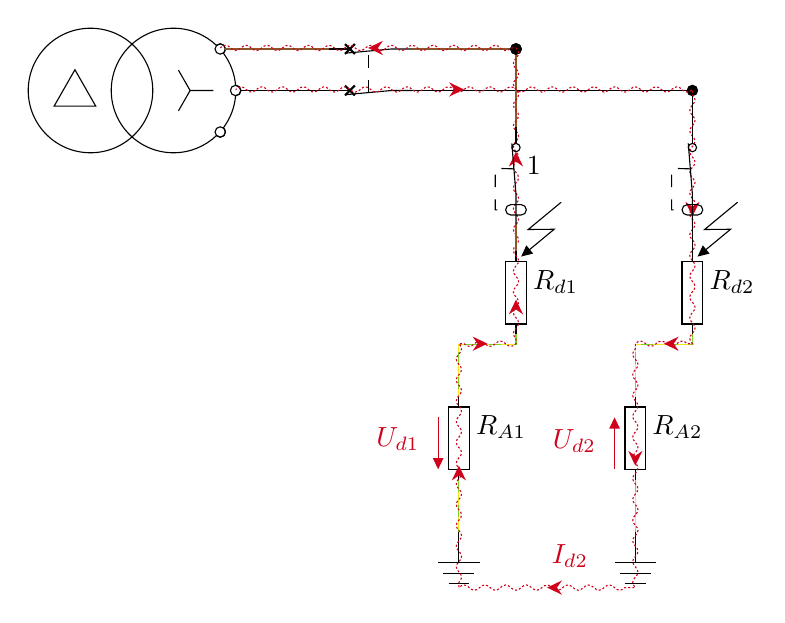
\begin{tikzpicture}[x=0.75pt,y=0.75pt,yscale=-1,xscale=1]
%uncomment if require: \path (0,314); %set diagram left start at 0, and has height of 314

%Straight Lines [id:da44771480202014247] 
\draw [color={rgb, 255:red, 0; green, 0; blue, 0 }  ,draw opacity=1 ]   (337.5,52.5) -- (337.5,35) ;
%Straight Lines [id:da5616221950341589] 
\draw    (202.5,35) -- (337.5,35) ;
%Straight Lines [id:da030139218122943512] 
\draw [color={rgb, 255:red, 139; green, 87; blue, 42 }  ,draw opacity=1 ]   (202.5,15) -- (252.5,15) ;
%Shape: Path Data [id:dp23022875443693058] 
\draw   (112.5,55) .. controls (112.5,56.38) and (111.38,57.5) .. (110,57.5) .. controls (109.29,57.5) and (108.65,57.2) .. (108.19,56.72) .. controls (102.81,61.85) and (95.52,65) .. (87.5,65) .. controls (70.93,65) and (57.5,51.57) .. (57.5,35) .. controls (57.5,18.43) and (70.93,5) .. (87.5,5) .. controls (95.52,5) and (102.81,8.15) .. (108.19,13.28) .. controls (108.65,12.8) and (109.29,12.5) .. (110,12.5) .. controls (111.38,12.5) and (112.5,13.62) .. (112.5,15) .. controls (112.5,15.82) and (112.11,16.54) .. (111.5,17) .. controls (114.8,21.39) and (116.92,26.71) .. (117.4,32.5) .. controls (117.43,32.5) and (117.47,32.5) .. (117.5,32.5) .. controls (118.88,32.5) and (120,33.62) .. (120,35) .. controls (120,36.38) and (118.88,37.5) .. (117.5,37.5) .. controls (117.47,37.5) and (117.43,37.5) .. (117.4,37.5) .. controls (116.92,43.29) and (114.8,48.61) .. (111.5,53) .. controls (112.11,53.46) and (112.5,54.18) .. (112.5,55) -- cycle ;
%Shape: Circle [id:dp1357901111827381] 
\draw   (17.5,35) .. controls (17.5,18.43) and (30.93,5) .. (47.5,5) .. controls (64.07,5) and (77.5,18.43) .. (77.5,35) .. controls (77.5,51.57) and (64.07,65) .. (47.5,65) .. controls (30.93,65) and (17.5,51.57) .. (17.5,35) -- cycle ;
%Shape: Triangle [id:dp7632621922673382] 
\draw   (40,25) -- (30,42.5) -- (50,42.5) -- cycle ;
%Shape: Star [id:dp9731649410229973] 
\draw   (106.75,35) -- (95.5,35) -- (89.88,44.81) -- (95.5,35) -- (89.88,25.19) -- (95.5,35) -- cycle ;
%Shape: Circle [id:dp31079836431690466] 
\draw   (107.5,15) .. controls (107.5,13.62) and (108.62,12.5) .. (110,12.5) .. controls (111.38,12.5) and (112.5,13.62) .. (112.5,15) .. controls (112.5,16.38) and (111.38,17.5) .. (110,17.5) .. controls (108.62,17.5) and (107.5,16.38) .. (107.5,15) -- cycle ;
%Shape: Circle [id:dp12266233820557082] 
\draw   (114.9,35) .. controls (114.9,33.62) and (116.02,32.5) .. (117.4,32.5) .. controls (118.78,32.5) and (119.9,33.62) .. (119.9,35) .. controls (119.9,36.38) and (118.78,37.5) .. (117.4,37.5) .. controls (116.02,37.5) and (114.9,36.38) .. (114.9,35) -- cycle ;
%Shape: Circle [id:dp5285901626538249] 
\draw   (107.5,55) .. controls (107.5,53.62) and (108.62,52.5) .. (110,52.5) .. controls (111.38,52.5) and (112.5,53.62) .. (112.5,55) .. controls (112.5,56.38) and (111.38,57.5) .. (110,57.5) .. controls (108.62,57.5) and (107.5,56.38) .. (107.5,55) -- cycle ;

%Straight Lines [id:da92188130951024] 
\draw [color={rgb, 255:red, 248; green, 231; blue, 28 }  ,draw opacity=1 ]   (225,222.5) -- (225,247.5) ;
%Straight Lines [id:da4292625671170487] 
\draw    (225,247.5) -- (225,262.5) ;
%Straight Lines [id:da06158937078168358] 
\draw    (215,262.5) -- (235,262.5) ;
%Straight Lines [id:da34789977188703036] 
\draw    (217.5,267.5) -- (232.5,267.5) ;
%Straight Lines [id:da1284483495628228] 
\draw    (220,272.5) -- (230,272.5) ;

%Straight Lines [id:da9082827551048067] 
\draw [color={rgb, 255:red, 126; green, 211; blue, 33 }  ,draw opacity=1 ] [dash pattern={on 4.5pt off 4.5pt}]  (225,222.5) -- (225,247.5) ;
%Straight Lines [id:da3209999402872329] 
\draw    (225,217.5) -- (225,222.5) ;
%Shape: Rectangle [id:dp2593386875607734] 
\draw   (230,187.5) -- (230,217.5) -- (220,217.5) -- (220,187.5) -- cycle ;
%Straight Lines [id:da740170600357607] 
\draw    (225,182.5) -- (225,187.5) ;

%Shape: Circle [id:dp8601483461254399] 
\draw  [fill={rgb, 255:red, 0; green, 0; blue, 0 }  ,fill opacity=1 ] (335,35) .. controls (335,33.62) and (336.12,32.5) .. (337.5,32.5) .. controls (338.88,32.5) and (340,33.62) .. (340,35) .. controls (340,36.38) and (338.88,37.5) .. (337.5,37.5) .. controls (336.12,37.5) and (335,36.38) .. (335,35) -- cycle ;
%Shape: Circle [id:dp12093020485396755] 
\draw  [fill={rgb, 255:red, 0; green, 0; blue, 0 }  ,fill opacity=1 ] (250,15) .. controls (250,13.62) and (251.12,12.5) .. (252.5,12.5) .. controls (253.88,12.5) and (255,13.62) .. (255,15) .. controls (255,16.38) and (253.88,17.5) .. (252.5,17.5) .. controls (251.12,17.5) and (250,16.38) .. (250,15) -- cycle ;
%Straight Lines [id:da2667129361258299] 
\draw [color={rgb, 255:red, 139; green, 87; blue, 42 }  ,draw opacity=1 ]   (112.5,15) -- (162.5,15) ;
%Straight Lines [id:da7247612407560878] 
\draw    (120,35) -- (162.5,35) ;
%Straight Lines [id:da9818089865990709] 
\draw    (310,217.5) -- (310,222.5) ;
%Shape: Rectangle [id:dp5739667555283554] 
\draw   (315,187.5) -- (315,217.5) -- (305,217.5) -- (305,187.5) -- cycle ;
%Straight Lines [id:da37673824938051304] 
\draw    (310,182.5) -- (310,187.5) ;

%Straight Lines [id:da9108771567706163] 
\draw [color={rgb, 255:red, 248; green, 231; blue, 28 }  ,draw opacity=1 ]   (310,222.5) -- (310,247.5) ;
%Straight Lines [id:da7506296134174059] 
\draw    (310,247.5) -- (310,262.5) ;
%Straight Lines [id:da8877376114904583] 
\draw    (300,262.5) -- (320,262.5) ;
%Straight Lines [id:da7805584248970565] 
\draw    (302.5,267.5) -- (317.5,267.5) ;
%Straight Lines [id:da4987046828919294] 
\draw    (305,272.5) -- (315,272.5) ;

%Straight Lines [id:da07069683992258613] 
\draw [color={rgb, 255:red, 126; green, 211; blue, 33 }  ,draw opacity=1 ] [dash pattern={on 4.5pt off 4.5pt}]  (310,222.5) -- (310,247.5) ;
%Shape: Boxed Line [id:dp017806634598713234] 
\draw    (274.27,88.83) -- (258.39,101.97) -- (270.89,101.86) -- (257.31,113.09) ;
\draw [shift={(255,115)}, rotate = 320.40999999999997] [fill={rgb, 255:red, 0; green, 0; blue, 0 }  ][line width=0.08]  [draw opacity=0] (5.36,-2.57) -- (0,0) -- (5.36,2.57) -- cycle    ;
%Shape: Boxed Line [id:dp8065003718686437] 
\draw    (359.27,88.83) -- (343.39,101.97) -- (355.89,101.86) -- (342.31,113.09) ;
\draw [shift={(340,115)}, rotate = 320.40999999999997] [fill={rgb, 255:red, 0; green, 0; blue, 0 }  ][line width=0.08]  [draw opacity=0] (5.36,-2.57) -- (0,0) -- (5.36,2.57) -- cycle    ;
%Straight Lines [id:da358454328833814] 
\draw    (170.5,37) -- (192.5,35) -- (202.5,35) ;
%Straight Lines [id:da868029205565597] 
\draw    (172.5,35) -- (162.5,35) ;
\draw [shift={(172.5,35)}, rotate = 225] [color={rgb, 255:red, 0; green, 0; blue, 0 }  ][line width=0.75]    (-3.35,0) -- (3.35,0)(0,3.35) -- (0,-3.35)   ;
%Straight Lines [id:da5656192330750602] 
\draw    (170.5,17) -- (192.5,15) -- (202.5,15) ;
%Straight Lines [id:da95863135682658] 
\draw  [dash pattern={on 4.5pt off 4.5pt}]  (181.5,36) -- (181.5,16) ;
%Straight Lines [id:da04894585565347964] 
\draw    (172.5,15) -- (162.5,15) ;
\draw [shift={(172.5,15)}, rotate = 225] [color={rgb, 255:red, 0; green, 0; blue, 0 }  ][line width=0.75]    (-3.35,0) -- (3.35,0)(0,3.35) -- (0,-3.35)   ;

%Straight Lines [id:da3293738134254155] 
\draw [color={rgb, 255:red, 139; green, 87; blue, 42 }  ,draw opacity=1 ]   (252.5,52.5) -- (252.5,15) ;
%Shape: Circle [id:dp8784736615935372] 
\draw  [fill={rgb, 255:red, 0; green, 0; blue, 0 }  ,fill opacity=1 ] (250,15) .. controls (250,13.62) and (251.12,12.5) .. (252.5,12.5) .. controls (253.88,12.5) and (255,13.62) .. (255,15) .. controls (255,16.38) and (253.88,17.5) .. (252.5,17.5) .. controls (251.12,17.5) and (250,16.38) .. (250,15) -- cycle ;
%Shape: Circle [id:dp11711924104585536] 
\draw  [fill={rgb, 255:red, 0; green, 0; blue, 0 }  ,fill opacity=1 ] (250,15) .. controls (250,13.62) and (251.12,12.5) .. (252.5,12.5) .. controls (253.88,12.5) and (255,13.62) .. (255,15) .. controls (255,16.38) and (253.88,17.5) .. (252.5,17.5) .. controls (251.12,17.5) and (250,16.38) .. (250,15) -- cycle ;
%Straight Lines [id:da08029921398538342] 
\draw    (252.5,147.5) -- (252.5,152.5) ;
%Shape: Rectangle [id:dp10461869500763998] 
\draw   (257.5,117.5) -- (257.5,147.5) -- (247.5,147.5) -- (247.5,117.5) -- cycle ;
%Straight Lines [id:da6711839663438437] 
\draw    (252.5,112.5) -- (252.5,117.5) ;

%Straight Lines [id:da306978016539733] 
\draw [color={rgb, 255:red, 208; green, 2; blue, 27 }  ,draw opacity=1 ]   (215,192.5) -- (215,214.5) ;
\draw [shift={(215,217.5)}, rotate = 270] [fill={rgb, 255:red, 208; green, 2; blue, 27 }  ,fill opacity=1 ][line width=0.08]  [draw opacity=0] (5.36,-2.57) -- (0,0) -- (5.36,2.57) -- cycle    ;
%Straight Lines [id:da9788903429329091] 
\draw [color={rgb, 255:red, 248; green, 231; blue, 28 }  ,draw opacity=1 ]   (252.5,152.5) -- (252.5,157.5) -- (225,157.5) -- (225,182.5) ;
%Straight Lines [id:da5746028122478745] 
\draw [color={rgb, 255:red, 126; green, 211; blue, 33 }  ,draw opacity=1 ] [dash pattern={on 4.5pt off 4.5pt}]  (252.5,152.5) -- (252.5,157.5) -- (225,157.5) -- (225,182.5) ;
%Straight Lines [id:da6637901588667133] 
\draw    (337.5,147.5) -- (337.5,152.5) ;
%Shape: Rectangle [id:dp33834418757589935] 
\draw   (342.5,117.5) -- (342.5,147.5) -- (332.5,147.5) -- (332.5,117.5) -- cycle ;
%Straight Lines [id:da4844708396236749] 
\draw    (337.5,112.5) -- (337.5,117.5) ;

%Straight Lines [id:da4767279022409927] 
\draw [color={rgb, 255:red, 208; green, 2; blue, 27 }  ,draw opacity=1 ]   (300,195.5) -- (300,217.5) ;
\draw [shift={(300,192.5)}, rotate = 90] [fill={rgb, 255:red, 208; green, 2; blue, 27 }  ,fill opacity=1 ][line width=0.08]  [draw opacity=0] (5.36,-2.57) -- (0,0) -- (5.36,2.57) -- cycle    ;
%Straight Lines [id:da015083238595793191] 
\draw [color={rgb, 255:red, 248; green, 231; blue, 28 }  ,draw opacity=1 ]   (337.5,152.5) -- (337.5,157.5) -- (310,157.5) -- (310,182.5) ;
%Straight Lines [id:da013265453939943717] 
\draw [color={rgb, 255:red, 126; green, 211; blue, 33 }  ,draw opacity=1 ] [dash pattern={on 4.5pt off 4.5pt}]  (337.5,152.5) -- (337.5,157.5) -- (310,157.5) -- (310,182.5) ;
%Straight Lines [id:da20369483289006973] 
\draw [color={rgb, 255:red, 208; green, 2; blue, 27 }  ,draw opacity=1 ] [dash pattern={on 0.75pt off 0.75pt}]  (110,14.5) .. controls (111.67,12.83) and (113.33,12.83) .. (115,14.5) .. controls (116.67,16.17) and (118.33,16.17) .. (120,14.5) .. controls (121.67,12.83) and (123.33,12.83) .. (125,14.5) .. controls (126.67,16.17) and (128.33,16.17) .. (130,14.5) .. controls (131.67,12.83) and (133.33,12.83) .. (135,14.5) .. controls (136.67,16.17) and (138.33,16.17) .. (140,14.5) .. controls (141.67,12.83) and (143.33,12.83) .. (145,14.5) .. controls (146.67,16.17) and (148.33,16.17) .. (150,14.5) .. controls (151.67,12.83) and (153.33,12.83) .. (155,14.5) .. controls (156.67,16.17) and (158.33,16.17) .. (160,14.5) .. controls (161.67,12.83) and (163.33,12.83) .. (165,14.5) .. controls (166.67,16.17) and (168.33,16.17) .. (170,14.5) .. controls (171.67,12.83) and (173.33,12.83) .. (175,14.5) .. controls (176.67,16.17) and (178.33,16.17) .. (180,14.5) .. controls (181.67,12.83) and (183.33,12.83) .. (185,14.5) .. controls (186.67,16.17) and (188.33,16.17) .. (190,14.5) .. controls (191.67,12.83) and (193.33,12.83) .. (195,14.5) .. controls (196.67,16.17) and (198.33,16.17) .. (200,14.5) .. controls (201.67,12.83) and (203.33,12.83) .. (205,14.5) .. controls (206.67,16.17) and (208.33,16.17) .. (210,14.5) .. controls (211.67,12.83) and (213.33,12.83) .. (215,14.5) .. controls (216.67,16.17) and (218.33,16.17) .. (220,14.5) .. controls (221.67,12.83) and (223.33,12.83) .. (225,14.5) .. controls (226.67,16.17) and (228.33,16.17) .. (230,14.5) .. controls (231.67,12.83) and (233.33,12.83) .. (235,14.5) .. controls (236.67,16.17) and (238.33,16.17) .. (240,14.5) .. controls (241.67,12.83) and (243.33,12.83) .. (245,14.5) .. controls (246.67,16.17) and (248.33,16.17) .. (250,14.5) -- (252.5,14.5) -- (252.5,14.5) .. controls (254.17,16.17) and (254.17,17.83) .. (252.5,19.5) .. controls (250.83,21.17) and (250.83,22.83) .. (252.5,24.5) .. controls (254.17,26.17) and (254.17,27.83) .. (252.5,29.5) .. controls (250.83,31.17) and (250.83,32.83) .. (252.5,34.5) .. controls (254.17,36.17) and (254.17,37.83) .. (252.5,39.5) .. controls (250.83,41.17) and (250.83,42.83) .. (252.5,44.5) .. controls (254.17,46.17) and (254.17,47.83) .. (252.5,49.5) .. controls (250.83,51.17) and (250.83,52.83) .. (252.5,54.5) .. controls (254.17,56.17) and (254.17,57.83) .. (252.5,59.5) .. controls (250.83,61.17) and (250.83,62.83) .. (252.5,64.5) .. controls (254.17,66.17) and (254.17,67.83) .. (252.5,69.5) .. controls (250.83,71.17) and (250.83,72.83) .. (252.5,74.5) .. controls (254.17,76.17) and (254.17,77.83) .. (252.5,79.5) .. controls (250.83,81.17) and (250.83,82.83) .. (252.5,84.5) .. controls (254.17,86.17) and (254.17,87.83) .. (252.5,89.5) .. controls (250.83,91.17) and (250.83,92.83) .. (252.5,94.5) .. controls (254.17,96.17) and (254.17,97.83) .. (252.5,99.5) .. controls (250.83,101.17) and (250.83,102.83) .. (252.5,104.5) .. controls (254.17,106.17) and (254.17,107.83) .. (252.5,109.5) .. controls (250.83,111.17) and (250.83,112.83) .. (252.5,114.5) -- (252.5,114.5) .. controls (254.17,116.17) and (254.17,117.83) .. (252.5,119.5) .. controls (250.83,121.17) and (250.83,122.83) .. (252.5,124.5) .. controls (254.17,126.17) and (254.17,127.83) .. (252.5,129.5) .. controls (250.83,131.17) and (250.83,132.83) .. (252.5,134.5) .. controls (254.17,136.17) and (254.17,137.83) .. (252.5,139.5) .. controls (250.83,141.17) and (250.83,142.83) .. (252.5,144.5) .. controls (254.17,146.17) and (254.17,147.83) .. (252.5,149.5) .. controls (250.83,151.17) and (250.83,152.83) .. (252.5,154.5) -- (252.5,157) -- (252.5,157) .. controls (250.83,158.67) and (249.17,158.67) .. (247.5,157) .. controls (245.83,155.33) and (244.17,155.33) .. (242.5,157) .. controls (240.83,158.67) and (239.17,158.67) .. (237.5,157) .. controls (235.83,155.33) and (234.17,155.33) .. (232.5,157) .. controls (230.83,158.67) and (229.17,158.67) .. (227.5,157) -- (225,157) -- (225,157) .. controls (226.67,158.67) and (226.67,160.33) .. (225,162) .. controls (223.33,163.67) and (223.33,165.33) .. (225,167) .. controls (226.67,168.67) and (226.67,170.33) .. (225,172) .. controls (223.33,173.67) and (223.33,175.33) .. (225,177) .. controls (226.67,178.67) and (226.67,180.33) .. (225,182) .. controls (223.33,183.67) and (223.33,185.33) .. (225,187) .. controls (226.67,188.67) and (226.67,190.33) .. (225,192) .. controls (223.33,193.67) and (223.33,195.33) .. (225,197) .. controls (226.67,198.67) and (226.67,200.33) .. (225,202) .. controls (223.33,203.67) and (223.33,205.33) .. (225,207) .. controls (226.67,208.67) and (226.67,210.33) .. (225,212) .. controls (223.33,213.67) and (223.33,215.33) .. (225,217) .. controls (226.67,218.67) and (226.67,220.33) .. (225,222) .. controls (223.33,223.67) and (223.33,225.33) .. (225,227) .. controls (226.67,228.67) and (226.67,230.33) .. (225,232) .. controls (223.33,233.67) and (223.33,235.33) .. (225,237) .. controls (226.67,238.67) and (226.67,240.33) .. (225,242) .. controls (223.33,243.67) and (223.33,245.33) .. (225,247) .. controls (226.67,248.67) and (226.67,250.33) .. (225,252) .. controls (223.33,253.67) and (223.33,255.33) .. (225,257) .. controls (226.67,258.67) and (226.67,260.33) .. (225,262) .. controls (223.33,263.67) and (223.33,265.33) .. (225,267) .. controls (226.67,268.67) and (226.67,270.33) .. (225,272) -- (225,274.5) -- (225,274.5) .. controls (226.67,272.83) and (228.33,272.83) .. (230,274.5) .. controls (231.67,276.17) and (233.33,276.17) .. (235,274.5) .. controls (236.67,272.83) and (238.33,272.83) .. (240,274.5) .. controls (241.67,276.17) and (243.33,276.17) .. (245,274.5) .. controls (246.67,272.83) and (248.33,272.83) .. (250,274.5) .. controls (251.67,276.17) and (253.33,276.17) .. (255,274.5) .. controls (256.67,272.83) and (258.33,272.83) .. (260,274.5) .. controls (261.67,276.17) and (263.33,276.17) .. (265,274.5) .. controls (266.67,272.83) and (268.33,272.83) .. (270,274.5) .. controls (271.67,276.17) and (273.33,276.17) .. (275,274.5) .. controls (276.67,272.83) and (278.33,272.83) .. (280,274.5) .. controls (281.67,276.17) and (283.33,276.17) .. (285,274.5) .. controls (286.67,272.83) and (288.33,272.83) .. (290,274.5) .. controls (291.67,276.17) and (293.33,276.17) .. (295,274.5) .. controls (296.67,272.83) and (298.33,272.83) .. (300,274.5) .. controls (301.67,276.17) and (303.33,276.17) .. (305,274.5) -- (310,274.5) -- (310,274.5) .. controls (308.33,272.83) and (308.33,271.17) .. (310,269.5) .. controls (311.67,267.83) and (311.67,266.17) .. (310,264.5) .. controls (308.33,262.83) and (308.33,261.17) .. (310,259.5) .. controls (311.67,257.83) and (311.67,256.17) .. (310,254.5) .. controls (308.33,252.83) and (308.33,251.17) .. (310,249.5) .. controls (311.67,247.83) and (311.67,246.17) .. (310,244.5) .. controls (308.33,242.83) and (308.33,241.17) .. (310,239.5) .. controls (311.67,237.83) and (311.67,236.17) .. (310,234.5) .. controls (308.33,232.83) and (308.33,231.17) .. (310,229.5) .. controls (311.67,227.83) and (311.67,226.17) .. (310,224.5) .. controls (308.33,222.83) and (308.33,221.17) .. (310,219.5) .. controls (311.67,217.83) and (311.67,216.17) .. (310,214.5) .. controls (308.33,212.83) and (308.33,211.17) .. (310,209.5) .. controls (311.67,207.83) and (311.67,206.17) .. (310,204.5) .. controls (308.33,202.83) and (308.33,201.17) .. (310,199.5) .. controls (311.67,197.83) and (311.67,196.17) .. (310,194.5) .. controls (308.33,192.83) and (308.33,191.17) .. (310,189.5) .. controls (311.67,187.83) and (311.67,186.17) .. (310,184.5) .. controls (308.33,182.83) and (308.33,181.17) .. (310,179.5) .. controls (311.67,177.83) and (311.67,176.17) .. (310,174.5) .. controls (308.33,172.83) and (308.33,171.17) .. (310,169.5) .. controls (311.67,167.83) and (311.67,166.17) .. (310,164.5) .. controls (308.33,162.83) and (308.33,161.17) .. (310,159.5) -- (310,157) -- (310,157) .. controls (311.67,155.33) and (313.33,155.33) .. (315,157) .. controls (316.67,158.67) and (318.33,158.67) .. (320,157) .. controls (321.67,155.33) and (323.33,155.33) .. (325,157) .. controls (326.67,158.67) and (328.33,158.67) .. (330,157) .. controls (331.67,155.33) and (333.33,155.33) .. (335,157) -- (337.5,157) -- (337.5,157) .. controls (335.83,155.33) and (335.83,153.67) .. (337.5,152) .. controls (339.17,150.33) and (339.17,148.67) .. (337.5,147) .. controls (335.83,145.33) and (335.83,143.67) .. (337.5,142) .. controls (339.17,140.33) and (339.17,138.67) .. (337.5,137) .. controls (335.83,135.33) and (335.83,133.67) .. (337.5,132) .. controls (339.17,130.33) and (339.17,128.67) .. (337.5,127) .. controls (335.83,125.33) and (335.83,123.67) .. (337.5,122) .. controls (339.17,120.33) and (339.17,118.67) .. (337.5,117) .. controls (335.83,115.33) and (335.83,113.67) .. (337.5,112) .. controls (339.17,110.33) and (339.17,108.67) .. (337.5,107) .. controls (335.83,105.33) and (335.83,103.67) .. (337.5,102) .. controls (339.17,100.33) and (339.17,98.67) .. (337.5,97) .. controls (335.83,95.33) and (335.83,93.67) .. (337.5,92) .. controls (339.17,90.33) and (339.17,88.67) .. (337.5,87) .. controls (335.83,85.33) and (335.83,83.67) .. (337.5,82) .. controls (339.17,80.33) and (339.17,78.67) .. (337.5,77) .. controls (335.83,75.33) and (335.83,73.67) .. (337.5,72) .. controls (339.17,70.33) and (339.17,68.67) .. (337.5,67) .. controls (335.83,65.33) and (335.83,63.67) .. (337.5,62) .. controls (339.17,60.33) and (339.17,58.67) .. (337.5,57) .. controls (335.83,55.33) and (335.83,53.67) .. (337.5,52) .. controls (339.17,50.33) and (339.17,48.67) .. (337.5,47) .. controls (335.83,45.33) and (335.83,43.67) .. (337.5,42) .. controls (339.17,40.33) and (339.17,38.67) .. (337.5,37) -- (337.5,34.5) -- (337.5,34.5) .. controls (335.83,36.17) and (334.17,36.17) .. (332.5,34.5) .. controls (330.83,32.83) and (329.17,32.83) .. (327.5,34.5) .. controls (325.83,36.17) and (324.17,36.17) .. (322.5,34.5) .. controls (320.83,32.83) and (319.17,32.83) .. (317.5,34.5) .. controls (315.83,36.17) and (314.17,36.17) .. (312.5,34.5) .. controls (310.83,32.83) and (309.17,32.83) .. (307.5,34.5) .. controls (305.83,36.17) and (304.17,36.17) .. (302.5,34.5) .. controls (300.83,32.83) and (299.17,32.83) .. (297.5,34.5) .. controls (295.83,36.17) and (294.17,36.17) .. (292.5,34.5) .. controls (290.83,32.83) and (289.17,32.83) .. (287.5,34.5) .. controls (285.83,36.17) and (284.17,36.17) .. (282.5,34.5) .. controls (280.83,32.83) and (279.17,32.83) .. (277.5,34.5) .. controls (275.83,36.17) and (274.17,36.17) .. (272.5,34.5) .. controls (270.83,32.83) and (269.17,32.83) .. (267.5,34.5) .. controls (265.83,36.17) and (264.17,36.17) .. (262.5,34.5) .. controls (260.83,32.83) and (259.17,32.83) .. (257.5,34.5) .. controls (255.83,36.17) and (254.17,36.17) .. (252.5,34.5) .. controls (250.83,32.83) and (249.17,32.83) .. (247.5,34.5) .. controls (245.83,36.17) and (244.17,36.17) .. (242.5,34.5) .. controls (240.83,32.83) and (239.17,32.83) .. (237.5,34.5) .. controls (235.83,36.17) and (234.17,36.17) .. (232.5,34.5) .. controls (230.83,32.83) and (229.17,32.83) .. (227.5,34.5) .. controls (225.83,36.17) and (224.17,36.17) .. (222.5,34.5) .. controls (220.83,32.83) and (219.17,32.83) .. (217.5,34.5) .. controls (215.83,36.17) and (214.17,36.17) .. (212.5,34.5) .. controls (210.83,32.83) and (209.17,32.83) .. (207.5,34.5) .. controls (205.83,36.17) and (204.17,36.17) .. (202.5,34.5) .. controls (200.83,32.83) and (199.17,32.83) .. (197.5,34.5) .. controls (195.83,36.17) and (194.17,36.17) .. (192.5,34.5) .. controls (190.83,32.83) and (189.17,32.83) .. (187.5,34.5) .. controls (185.83,36.17) and (184.17,36.17) .. (182.5,34.5) .. controls (180.83,32.83) and (179.17,32.83) .. (177.5,34.5) .. controls (175.83,36.17) and (174.17,36.17) .. (172.5,34.5) .. controls (170.83,32.83) and (169.17,32.83) .. (167.5,34.5) .. controls (165.83,36.17) and (164.17,36.17) .. (162.5,34.5) .. controls (160.83,32.83) and (159.17,32.83) .. (157.5,34.5) .. controls (155.83,36.17) and (154.17,36.17) .. (152.5,34.5) .. controls (150.83,32.83) and (149.17,32.83) .. (147.5,34.5) .. controls (145.83,36.17) and (144.17,36.17) .. (142.5,34.5) .. controls (140.83,32.83) and (139.17,32.83) .. (137.5,34.5) .. controls (135.83,36.17) and (134.17,36.17) .. (132.5,34.5) .. controls (130.83,32.83) and (129.17,32.83) .. (127.5,34.5) .. controls (125.83,36.17) and (124.17,36.17) .. (122.5,34.5) .. controls (120.83,32.83) and (119.17,32.83) .. (117.5,34.5) -- (117.4,34.5) -- (117.4,34.5) ;
\draw [shift={(181.25,14.5)}, rotate = 0] [fill={rgb, 255:red, 208; green, 2; blue, 27 }  ,fill opacity=1 ][line width=0.08]  [draw opacity=0] (7.14,-3.43) -- (0,0) -- (7.14,3.43) -- (4.74,0) -- cycle    ;
\draw [shift={(252.5,64.5)}, rotate = 90] [fill={rgb, 255:red, 208; green, 2; blue, 27 }  ,fill opacity=1 ][line width=0.08]  [draw opacity=0] (7.14,-3.43) -- (0,0) -- (7.14,3.43) -- (4.74,0) -- cycle    ;
\draw [shift={(252.5,135.75)}, rotate = 90] [fill={rgb, 255:red, 208; green, 2; blue, 27 }  ,fill opacity=1 ][line width=0.08]  [draw opacity=0] (7.14,-3.43) -- (0,0) -- (7.14,3.43) -- (4.74,0) -- cycle    ;
\draw [shift={(238.75,157)}, rotate = 180] [fill={rgb, 255:red, 208; green, 2; blue, 27 }  ,fill opacity=1 ][line width=0.08]  [draw opacity=0] (7.14,-3.43) -- (0,0) -- (7.14,3.43) -- (4.74,0) -- cycle    ;
\draw [shift={(225,215.75)}, rotate = 90] [fill={rgb, 255:red, 208; green, 2; blue, 27 }  ,fill opacity=1 ][line width=0.08]  [draw opacity=0] (7.14,-3.43) -- (0,0) -- (7.14,3.43) -- (4.74,0) -- cycle    ;
\draw [shift={(267.5,274.5)}, rotate = 0] [fill={rgb, 255:red, 208; green, 2; blue, 27 }  ,fill opacity=1 ][line width=0.08]  [draw opacity=0] (7.14,-3.43) -- (0,0) -- (7.14,3.43) -- (4.74,0) -- cycle    ;
\draw [shift={(310,215.75)}, rotate = 270] [fill={rgb, 255:red, 208; green, 2; blue, 27 }  ,fill opacity=1 ][line width=0.08]  [draw opacity=0] (7.14,-3.43) -- (0,0) -- (7.14,3.43) -- (4.74,0) -- cycle    ;
\draw [shift={(323.75,157)}, rotate = 0] [fill={rgb, 255:red, 208; green, 2; blue, 27 }  ,fill opacity=1 ][line width=0.08]  [draw opacity=0] (7.14,-3.43) -- (0,0) -- (7.14,3.43) -- (4.74,0) -- cycle    ;
\draw [shift={(337.5,95.75)}, rotate = 270] [fill={rgb, 255:red, 208; green, 2; blue, 27 }  ,fill opacity=1 ][line width=0.08]  [draw opacity=0] (7.14,-3.43) -- (0,0) -- (7.14,3.43) -- (4.74,0) -- cycle    ;
\draw [shift={(227.45,34.5)}, rotate = 180] [fill={rgb, 255:red, 208; green, 2; blue, 27 }  ,fill opacity=1 ][line width=0.08]  [draw opacity=0] (7.14,-3.43) -- (0,0) -- (7.14,3.43) -- (4.74,0) -- cycle    ;
%Shape: Circle [id:dp6688360070263407] 
\draw   (254.5,62.5) .. controls (254.5,61.4) and (253.6,60.5) .. (252.5,60.5) .. controls (251.4,60.5) and (250.5,61.4) .. (250.5,62.5) .. controls (250.5,63.6) and (251.4,64.5) .. (252.5,64.5) .. controls (253.6,64.5) and (254.5,63.6) .. (254.5,62.5) -- cycle ;
%Straight Lines [id:da023498503244457125] 
\draw    (252.5,60.5) -- (252.5,52.5) ;
%Rounded Rect [id:dp30279070557566734] 
\draw   (247.5,92.5) .. controls (247.5,91.12) and (248.62,90) .. (250,90) -- (255,90) .. controls (256.38,90) and (257.5,91.12) .. (257.5,92.5) -- (257.5,92.5) .. controls (257.5,93.88) and (256.38,95) .. (255,95) -- (250,95) .. controls (248.62,95) and (247.5,93.88) .. (247.5,92.5) -- cycle ;
%Straight Lines [id:da16468651371944532] 
\draw  [dash pattern={on 4.5pt off 4.5pt}]  (251.5,72.75) -- (242.5,72.5) -- (242.5,92.5) -- (247.5,92.5) ;
%Straight Lines [id:da8036936912023739] 
\draw    (250.5,60.5) -- (252.5,85) -- (252.5,100) ;

%Shape: Circle [id:dp7937625551850244] 
\draw   (339.5,62.5) .. controls (339.5,61.4) and (338.6,60.5) .. (337.5,60.5) .. controls (336.4,60.5) and (335.5,61.4) .. (335.5,62.5) .. controls (335.5,63.6) and (336.4,64.5) .. (337.5,64.5) .. controls (338.6,64.5) and (339.5,63.6) .. (339.5,62.5) -- cycle ;
%Straight Lines [id:da5242903170497772] 
\draw    (337.5,60.5) -- (337.5,52.5) ;
%Rounded Rect [id:dp6818768532487535] 
\draw   (332.5,92.5) .. controls (332.5,91.12) and (333.62,90) .. (335,90) -- (340,90) .. controls (341.38,90) and (342.5,91.12) .. (342.5,92.5) -- (342.5,92.5) .. controls (342.5,93.88) and (341.38,95) .. (340,95) -- (335,95) .. controls (333.62,95) and (332.5,93.88) .. (332.5,92.5) -- cycle ;
%Straight Lines [id:da0851882978686429] 
\draw  [dash pattern={on 4.5pt off 4.5pt}]  (336.5,72.75) -- (327.5,72.5) -- (327.5,92.5) -- (332.5,92.5) ;
%Straight Lines [id:da2719116658142192] 
\draw    (335.5,60.5) -- (337.5,85) -- (337.5,100) ;

%Straight Lines [id:da23106759511180686] 
\draw [color={rgb, 255:red, 139; green, 87; blue, 42 }  ,draw opacity=1 ]   (252.5,112.5) -- (252.5,100) ;
%Straight Lines [id:da04628877500711526] 
\draw [color={rgb, 255:red, 0; green, 0; blue, 0 }  ,draw opacity=1 ]   (337.5,112.5) -- (337.5,100) ;


% Text Node
\draw (232,190.5) node [anchor=north west][inner sep=0.75pt]   [align=left] {$R_{A1}$};
% Text Node
\draw (317,190.5) node [anchor=north west][inner sep=0.75pt]   [align=left] {$R_{A2}$};
% Text Node
\draw (268.5,252.5) node [anchor=north west][inner sep=0.75pt]  [color={rgb, 255:red, 208; green, 2; blue, 27 }  ,opacity=1 ] [align=left] {$I_{d2}$};
% Text Node
\draw (184,196) node [anchor=north west][inner sep=0.75pt]  [color={rgb, 255:red, 208; green, 2; blue, 27 }  ,opacity=1 ] [align=left] {$U_{d1}$};
% Text Node
\draw (259.5,120.5) node [anchor=north west][inner sep=0.75pt]   [align=left] {$R_{d1}$};
% Text Node
\draw (269,197) node [anchor=north west][inner sep=0.75pt]  [color={rgb, 255:red, 208; green, 2; blue, 27 }  ,opacity=1 ] [align=left] {$U_{d2}$};
% Text Node
\draw (344.5,120.5) node [anchor=north west][inner sep=0.75pt]   [align=left] {$R_{d2}$};
% Text Node
\draw (256.5,65.5) node [anchor=north west][inner sep=0.75pt]   [align=left] {\Circled{1}};

\end{tikzpicture}


\end{figure}

%\end{document}


L'intensité de courant $I_{d2}$ vaut alors :
\begin{formule}{Courant du deuxième défaut $I_{d2}$ en schéma Isolé-Individuel}{}
\begin{align*}
		I_{d2} &= \frac{U}{R_{d1}+R_{A1}+R_{A2}+R_{A2}} \\
\end{align*}

\begin{textvariables}
U								& tension nominale composée				& volt			& \volt					& 	Différence de potentiel entre deux conducteurs actifs (à préciser s'il s'agit du conducteur neutre)	\\
R_{d1}						& résistance											& ohm			& \ohm					& 	Résistance de défaut 	d'isolement de l'appareil 1\\
R_{A1}						& résistance											& ohm			& \ohm					& 	Résistance de la prise de terre de l'appareil 1 	\\
R_{A2}						& résistance											& ohm			& \ohm					& 	Résistance de la prise de terre de l'appareil 2 	\\
R_{d2}						& résistance											& ohm			& \ohm					& 	Résistance de défaut 	d'isolement de l'appareil 1\\
\end{textvariables}
\end{formule}

Le courant de défaut $I_{d1}$ fera alors apparaître une \emph{tension de défaut} $U_{d1}$ entre la masse métallique de l'appareil 1 et la terre. Cette tension, limitée par l'impédance de fuite, sera très largement inférieure à  $U_L$ et ne sera donc pas dangereuse. La situation sera similaire avec un schéma Impédant-Individuel $Z_N$, ou l'impédance de limitation limitera également le courant de défaut :

\begin{formule}{Tension de défaut $U_{d1}$ en schéma Isolé-Individuel}{}
\begin{align*}
		U_{d1} &= R_{A1} \times I_{d2} \\
					&<	U_L
\end{align*}

\begin{textvariables}
R_{A1}						& résistance											& ohm			& \ohm					& 	Résistance de la prise de terre de l'appareil 1 	\\
I_{d2}						& intensité												& ampère		& \ampere				& 	Courant de défaut de l'appareil 2 \\
U_{L}						& tension							& volt			& \volt										& 	Tension de sécurité du local avec :
\begin{description}[nosep, leftmargin=*]
\item[Local sec :] $U_{L}=\SI{50}{\volt}$
\item[Local humide :] $U_{L}=\SI{25}{\volt}$
\end{description} \\
\end{textvariables}
\end{formule}

Le cas est similaire à ceux rencontrés en schéma TT, on procèdera de la même manière en protégeant chaque groupe de masses par un DDR au calibre adapté \Circled{1}. Il est donc nécessaire de limiter $U_{d1}$ à la valeur suivante (voir \superref{form:resistance_prise_terre}) :

\begin{formule*}{Calibre du DDR $I_{\Delta n}$}{}
\begin{align*}
		I_{\Delta n} &< \frac{U_{L}}{R_{A1}}
\end{align*}

\begin{textvariables}
R_{A1}						& résistance											& ohm			& \ohm					& 	Résistance de la prise de terre de l'appareil 1 	\\
U_{L}						& tension							& volt			& \volt					& 	Tension de sécurité du local avec :
\begin{description}[nosep, leftmargin=*]
\item[Local sec :] $U_{L}=\SI{50}{\volt}$
\item[Local humide :] $U_{L}=\SI{25}{\volt}$
\end{description} \\
R_{A1}						& résistance											& ohm			& \ohm					& 	Résistance de la prise de terre de l'appareil 1 	\\
\end{textvariables}
\end{formule*}

L'usage de DDR implique de tenir du courant du premier défaut d'isolement $I_{d1}$ afin que la protection ne coupe pas le circuit dès le premier défaut :

\begin{table}[h]
\caption{Correspondance entre la capacité de fuite et le courant de premier défaut d'isolement}
\begin{tabular}{cc}
\toprule
\thead{Capacité de fuite (\si{\micro\farad})} 	&	\thead{Courant de premier défaut (\si{\ampere})} \\
\midrule
1		&	0,07 \\
5		& 0,36 \\
30		& 2,17 \\
\bottomrule
\end{tabular}
\end{table}
\begin{exemple}{Tension de défaut $U_{d1}$ en schéma Isolé-Individuel au deuxième défaut}{}
Si on considère que le transformateur est un transformateur $\SI{20}{\kilo\volt}/\SI{400}{\volt}$, que $R_{A1}=R_{A2}=\SI{40}{\ohm}$ et que $R_{d1} =R_{d1}= \SI{2}{\ohm}$, on peut déduire que le courant de défaut $I_{d2}$ vaut :
\begin{align*}
		I_{d2} &= \frac{U}{R_{d1}+R_{A1}+R_{A2}+R_{A2}} \\
					&=\frac{400}{2+40+40+2} \\
				&= \SI{4,76}{\ampere} \\
\end{align*}
Si une personne touche à la masse du récepteur 1, elle sera soumise à une tension de défaut $U_{d1}$ :
\begin{align*}
		U_{d1} &= R_{A1} \times I_{d2} \\
				&=40 \times 4,76 \\
				&= \SI{190,4}{\volt}
\end{align*}
La tension de défaut $U_{d1}$ est dangereuse quelle que soit la tension limite choisie :
\begin{itemize}
\item coupure la plus rapide possible\,;
\item protection des personnes.
\end{itemize}
~\\
\begin{minipage}[t]{0.5\linewidth}
Dans le cas d'un local sec :
\begin{align*}
	I_{\Delta n} 	&< \frac{U_{L}}{R_{A1}} \\
						&< \frac{50}{40} \\
						&< \SI{1,25}{\ampere}
\end{align*}
\end{minipage}
\hfill
\begin{minipage}[t]{0.5\linewidth}
Dans le cas d'un local humide :
\begin{align*}
	I_{\Delta n} 	&< \frac{U_{L}}{R_{A1}} \\
						&< \frac{25}{40} \\
						&< \SI{0,625}{\ampere}
\end{align*}
\end{minipage}
~\\
D'après le tableau situé en \superref{tab:temps_coupure_DDR}, le DDR protégeant la carcasse de l'appareil 1 doit présenter un temps de coupure de moins de \SI{200}{\milli\second} avec une tension de défaut $U_d$ de \SI{190,4}{\volt}.
\end{exemple}

\subsection{Neutre isolé et masses interconnectées et mise à la terre}

Les situations saines et au premier défaut d'isolement d'une installation en schéma IT avec les masses conductrices interconnectées et reliés en un seul point seront similaires au schéma IT avec les masses mise à la terre individuellement. Au deuxième défaut d'isolement, la situation sera différente, la prise en charge du défaut va s'apparenter à celle qu'on rencontre en schéma TN avec l'apparition d'un court-circuit.

 \begin{figure}[H]
\caption{Installation Isolé-Interconnectée}
\begin{subfigure}[t]{0.49\linewidth}
%--------------------------------------
%ELECTROTECHNIQUE - SCHEMA DE LIAISON A LA TERRE
%--------------------------------------

%utiliser les environnement \begin{comment} \end{comment} pour mettre en commentaire le préambule une fois la programmation appelée dans le document maître (!ne pas oublier de mettre en commentaire \end{document}!)

\begin{comment}

\documentclass[a4paper, 11pt, twoside, fleqn]{memoir}

\usepackage{AOCDTF}

\marqueurchapitre
\decoupagechapitre{1} %juste pour éviter les erreurs lors de la compilation des sous-programmations (passera en commentaire)

%lien d'édition des figures Tikz sur le site mathcha.io (rajouter le lien d'une modification effectuée sur la figure tikz avec le nom du modificateur car il n'y a qu'un lien par compte)

%lien mathcha Bruno Douchy : https://www.mathcha.io/editor/DXXG1FgjiNJCe0yo2ZTqzEeM8hlg57ygtvk5Mpy

%--------------------------------------
%corps du document
%--------------------------------------

\begin{document} %corps du document
	\openleft %début de chapitre à gauche

\end{comment}






% Pattern Info
 
\tikzset{
pattern size/.store in=\mcSize, 
pattern size = 5pt,
pattern thickness/.store in=\mcThickness, 
pattern thickness = 0.3pt,
pattern radius/.store in=\mcRadius, 
pattern radius = 1pt}
\makeatletter
\pgfutil@ifundefined{pgf@pattern@name@_kig45mqly}{
\pgfdeclarepatternformonly[\mcThickness,\mcSize]{_kig45mqly}
{\pgfqpoint{0pt}{0pt}}
{\pgfpoint{\mcSize+\mcThickness}{\mcSize+\mcThickness}}
{\pgfpoint{\mcSize}{\mcSize}}
{
\pgfsetcolor{\tikz@pattern@color}
\pgfsetlinewidth{\mcThickness}
\pgfpathmoveto{\pgfqpoint{0pt}{0pt}}
\pgfpathlineto{\pgfpoint{\mcSize+\mcThickness}{\mcSize+\mcThickness}}
\pgfusepath{stroke}
}}
\makeatother
\tikzset{every picture/.style={line width=0.5pt}} %set default line width to 0.75pt        

\begin{tikzpicture}[x=0.75pt,y=0.75pt,yscale=-0.6,xscale=0.6]
%uncomment if require: \path (0,293); %set diagram left start at 0, and has height of 293

%Straight Lines [id:da7855603359005625] 
\draw [color={rgb, 255:red, 74; green, 144; blue, 226 }  ,draw opacity=1 ]   (202.5,75.5) -- (462.5,75) ;
%Straight Lines [id:da3845932965061506] 
\draw [color={rgb, 255:red, 74; green, 144; blue, 226 }  ,draw opacity=1 ]   (90,75) -- (162.5,75) ;
%Straight Lines [id:da5834167633542386] 
\draw [color={rgb, 255:red, 248; green, 231; blue, 28 }  ,draw opacity=1 ]   (87.5,75) -- (27.5,75) -- (27.5,182.5) ;
%Straight Lines [id:da9429513177603445] 
\draw [color={rgb, 255:red, 248; green, 231; blue, 28 }  ,draw opacity=1 ]   (95.5,35) -- (87.5,75) -- (87.5,107.5) ;
%Straight Lines [id:da7600472701317061] 
\draw [color={rgb, 255:red, 126; green, 211; blue, 33 }  ,draw opacity=1 ] [dash pattern={on 2.25pt off 2.25pt}]  (95.5,35) -- (87.5,75) -- (87.5,107.5) ;
%Straight Lines [id:da6079599273540643] 
\draw [color={rgb, 255:red, 248; green, 231; blue, 28 }  ,draw opacity=1 ]   (240,135) -- (225,135) -- (225,182.5) ;
%Straight Lines [id:da8706050361736538] 
\draw    (202.5,35) -- (463.75,35) ;
%Straight Lines [id:da5697476802363065] 
\draw [color={rgb, 255:red, 139; green, 87; blue, 42 }  ,draw opacity=1 ]   (202.5,15) -- (462.5,15) ;
%Straight Lines [id:da9735954426571896] 
\draw [color={rgb, 255:red, 155; green, 155; blue, 155 }  ,draw opacity=1 ]   (202.5,55) -- (462.5,55) ;
%Shape: Path Data [id:dp36735613758138397] 
\draw   (112.5,55) .. controls (112.5,56.38) and (111.38,57.5) .. (110,57.5) .. controls (109.29,57.5) and (108.65,57.2) .. (108.19,56.72) .. controls (102.81,61.85) and (95.52,65) .. (87.5,65) .. controls (70.93,65) and (57.5,51.57) .. (57.5,35) .. controls (57.5,18.43) and (70.93,5) .. (87.5,5) .. controls (95.52,5) and (102.81,8.15) .. (108.19,13.28) .. controls (108.65,12.8) and (109.29,12.5) .. (110,12.5) .. controls (111.38,12.5) and (112.5,13.62) .. (112.5,15) .. controls (112.5,15.82) and (112.11,16.54) .. (111.5,17) .. controls (114.8,21.39) and (116.92,26.71) .. (117.4,32.5) .. controls (117.43,32.5) and (117.47,32.5) .. (117.5,32.5) .. controls (118.88,32.5) and (120,33.62) .. (120,35) .. controls (120,36.38) and (118.88,37.5) .. (117.5,37.5) .. controls (117.47,37.5) and (117.43,37.5) .. (117.4,37.5) .. controls (116.92,43.29) and (114.8,48.61) .. (111.5,53) .. controls (112.11,53.46) and (112.5,54.18) .. (112.5,55) -- cycle ;
%Shape: Circle [id:dp23421524241037028] 
\draw   (17.5,35) .. controls (17.5,18.43) and (30.93,5) .. (47.5,5) .. controls (64.07,5) and (77.5,18.43) .. (77.5,35) .. controls (77.5,51.57) and (64.07,65) .. (47.5,65) .. controls (30.93,65) and (17.5,51.57) .. (17.5,35) -- cycle ;
%Shape: Triangle [id:dp48236106138172463] 
\draw   (40,25) -- (30,42.5) -- (50,42.5) -- cycle ;
%Shape: Star [id:dp8682414008103251] 
\draw   (106.75,35) -- (95.5,35) -- (89.88,44.81) -- (95.5,35) -- (89.88,25.19) -- (95.5,35) -- cycle ;
%Shape: Circle [id:dp74403652528276] 
\draw   (107.5,15) .. controls (107.5,13.62) and (108.62,12.5) .. (110,12.5) .. controls (111.38,12.5) and (112.5,13.62) .. (112.5,15) .. controls (112.5,16.38) and (111.38,17.5) .. (110,17.5) .. controls (108.62,17.5) and (107.5,16.38) .. (107.5,15) -- cycle ;
%Shape: Circle [id:dp12230623178485356] 
\draw   (114.9,35) .. controls (114.9,33.62) and (116.02,32.5) .. (117.4,32.5) .. controls (118.78,32.5) and (119.9,33.62) .. (119.9,35) .. controls (119.9,36.38) and (118.78,37.5) .. (117.4,37.5) .. controls (116.02,37.5) and (114.9,36.38) .. (114.9,35) -- cycle ;
%Shape: Circle [id:dp8868519788786934] 
\draw   (107.5,55) .. controls (107.5,53.62) and (108.62,52.5) .. (110,52.5) .. controls (111.38,52.5) and (112.5,53.62) .. (112.5,55) .. controls (112.5,56.38) and (111.38,57.5) .. (110,57.5) .. controls (108.62,57.5) and (107.5,56.38) .. (107.5,55) -- cycle ;

%Straight Lines [id:da4565704928737364] 
\draw [color={rgb, 255:red, 74; green, 144; blue, 226 }  ,draw opacity=1 ]   (292.5,112.5) -- (292.5,77.5) ;
%Straight Lines [id:da08957212555201388] 
\draw [color={rgb, 255:red, 139; green, 87; blue, 42 }  ,draw opacity=1 ]   (252.5,112.5) -- (252.5,17.5) ;
%Straight Lines [id:da7418535885736515] 
\draw [color={rgb, 255:red, 139; green, 87; blue, 42 }  ,draw opacity=1 ]   (252.5,130) -- (252.5,117.5) ;
%Straight Lines [id:da8720965180296373] 
\draw [color={rgb, 255:red, 74; green, 144; blue, 226 }  ,draw opacity=1 ]   (292.5,130.5) -- (292.5,117.5) ;
%Straight Lines [id:da938936503356733] 
\draw    (17.5,232.5) -- (460,232.5) ;
%Shape: Rectangle [id:dp7311273665746781] 
\draw  [draw opacity=0][pattern=_kig45mqly,pattern size=6pt,pattern thickness=0.75pt,pattern radius=0pt, pattern color={rgb, 255:red, 0; green, 0; blue, 0}][line width=0.75]  (17.5,232.5) -- (460,232.5) -- (460,247.5) -- (17.5,247.5) -- cycle ;
%Straight Lines [id:da8141513336558377] 
\draw [color={rgb, 255:red, 126; green, 211; blue, 33 }  ,draw opacity=1 ] [dash pattern={on 2.25pt off 2.25pt}]  (240,135) -- (225,135) -- (225,182.5) ;
%Straight Lines [id:da29843762221307424] 
\draw [color={rgb, 255:red, 248; green, 231; blue, 28 }  ,draw opacity=1 ]   (225,222.5) -- (225,247.5) ;
%Straight Lines [id:da11084730612327653] 
\draw    (225,247.5) -- (225,262.5) ;
%Straight Lines [id:da28813972378566177] 
\draw    (215,262.5) -- (235,262.5) ;
%Straight Lines [id:da12034369105457465] 
\draw    (217.5,267.5) -- (232.5,267.5) ;
%Straight Lines [id:da6195695090232725] 
\draw    (220,272.5) -- (230,272.5) ;

%Straight Lines [id:da7010427793052417] 
\draw [color={rgb, 255:red, 126; green, 211; blue, 33 }  ,draw opacity=1 ] [dash pattern={on 2.25pt off 2.25pt}]  (225,222.5) -- (225,247.5) ;
%Straight Lines [id:da6639632595865842] 
\draw    (287.5,130) -- (292.5,130) ;
%Shape: Rectangle [id:dp48750397418832736] 
\draw   (257.5,125) -- (287.5,125) -- (287.5,135) -- (257.5,135) -- cycle ;
%Straight Lines [id:da3091869002192609] 
\draw    (252.5,130) -- (257.5,130) ;

%Straight Lines [id:da46843421066318236] 
\draw    (225,217.5) -- (225,222.5) ;
%Shape: Rectangle [id:dp8288861680700458] 
\draw   (230,187.5) -- (230,217.5) -- (220,217.5) -- (220,187.5) -- cycle ;
%Straight Lines [id:da39538233114745247] 
\draw    (225,182.5) -- (225,187.5) ;

%Straight Lines [id:da03908999537683522] 
\draw [color={rgb, 255:red, 74; green, 144; blue, 226 }  ,draw opacity=1 ]   (377.5,112.5) -- (377.5,77.5) ;
%Straight Lines [id:da014322617412467653] 
\draw [color={rgb, 255:red, 0; green, 0; blue, 0 }  ,draw opacity=1 ]   (337.5,112.5) -- (337.5,35) ;
%Straight Lines [id:da7075832342481658] 
\draw [color={rgb, 255:red, 139; green, 87; blue, 42 }  ,draw opacity=1 ]   (337.5,130) -- (337.5,117.5) ;
%Straight Lines [id:da37678293812005714] 
\draw [color={rgb, 255:red, 74; green, 144; blue, 226 }  ,draw opacity=1 ]   (377.5,130.5) -- (377.5,117.5) ;
%Straight Lines [id:da9817945211819089] 
\draw    (372.5,130) -- (377.5,130) ;
%Shape: Rectangle [id:dp3965217784422401] 
\draw   (342.5,125) -- (372.5,125) -- (372.5,135) -- (342.5,135) -- cycle ;
%Straight Lines [id:da03329133725543032] 
\draw    (337.5,130) -- (342.5,130) ;

%Straight Lines [id:da8796176191529531] 
\draw [color={rgb, 255:red, 74; green, 144; blue, 226 }  ,draw opacity=1 ]   (462.5,112.5) -- (462.5,77.5) ;
%Straight Lines [id:da6222130388950533] 
\draw [color={rgb, 255:red, 155; green, 155; blue, 155 }  ,draw opacity=1 ]   (422.5,112.5) -- (422.5,55) ;
%Straight Lines [id:da1963014933165811] 
\draw [color={rgb, 255:red, 139; green, 87; blue, 42 }  ,draw opacity=1 ]   (422.5,130) -- (422.5,117.5) ;
%Straight Lines [id:da25889379629104303] 
\draw [color={rgb, 255:red, 74; green, 144; blue, 226 }  ,draw opacity=1 ]   (462.5,130.5) -- (462.5,117.5) ;
%Straight Lines [id:da3869416860630762] 
\draw    (457.5,130) -- (462.5,130) ;
%Shape: Rectangle [id:dp6819736010368719] 
\draw   (427.5,125) -- (457.5,125) -- (457.5,135) -- (427.5,135) -- cycle ;
%Straight Lines [id:da34290626385752987] 
\draw    (422.5,130) -- (427.5,130) ;

%Shape: Circle [id:dp7660888532599164] 
\draw  [fill={rgb, 255:red, 0; green, 0; blue, 0 }  ,fill opacity=1 ] (375,75) .. controls (375,73.62) and (376.12,72.5) .. (377.5,72.5) .. controls (378.88,72.5) and (380,73.62) .. (380,75) .. controls (380,76.38) and (378.88,77.5) .. (377.5,77.5) .. controls (376.12,77.5) and (375,76.38) .. (375,75) -- cycle ;
%Shape: Circle [id:dp6916920109792153] 
\draw  [fill={rgb, 255:red, 0; green, 0; blue, 0 }  ,fill opacity=1 ] (460,75) .. controls (460,73.62) and (461.12,72.5) .. (462.5,72.5) .. controls (463.88,72.5) and (465,73.62) .. (465,75) .. controls (465,76.38) and (463.88,77.5) .. (462.5,77.5) .. controls (461.12,77.5) and (460,76.38) .. (460,75) -- cycle ;
%Shape: Circle [id:dp27655045875256845] 
\draw  [fill={rgb, 255:red, 0; green, 0; blue, 0 }  ,fill opacity=1 ] (335,35) .. controls (335,33.62) and (336.12,32.5) .. (337.5,32.5) .. controls (338.88,32.5) and (340,33.62) .. (340,35) .. controls (340,36.38) and (338.88,37.5) .. (337.5,37.5) .. controls (336.12,37.5) and (335,36.38) .. (335,35) -- cycle ;
%Shape: Circle [id:dp8031492541807427] 
\draw  [fill={rgb, 255:red, 0; green, 0; blue, 0 }  ,fill opacity=1 ] (420,55) .. controls (420,53.62) and (421.12,52.5) .. (422.5,52.5) .. controls (423.88,52.5) and (425,53.62) .. (425,55) .. controls (425,56.38) and (423.88,57.5) .. (422.5,57.5) .. controls (421.12,57.5) and (420,56.38) .. (420,55) -- cycle ;
%Shape: Circle [id:dp9192263751877222] 
\draw  [fill={rgb, 255:red, 0; green, 0; blue, 0 }  ,fill opacity=1 ] (290,75) .. controls (290,73.62) and (291.12,72.5) .. (292.5,72.5) .. controls (293.88,72.5) and (295,73.62) .. (295,75) .. controls (295,76.38) and (293.88,77.5) .. (292.5,77.5) .. controls (291.12,77.5) and (290,76.38) .. (290,75) -- cycle ;
%Shape: Circle [id:dp3725249444527118] 
\draw  [fill={rgb, 255:red, 0; green, 0; blue, 0 }  ,fill opacity=1 ] (250,15) .. controls (250,13.62) and (251.12,12.5) .. (252.5,12.5) .. controls (253.88,12.5) and (255,13.62) .. (255,15) .. controls (255,16.38) and (253.88,17.5) .. (252.5,17.5) .. controls (251.12,17.5) and (250,16.38) .. (250,15) -- cycle ;
%Shape: Rectangle [id:dp06629411116627981] 
\draw  [dash pattern={on 2.25pt off 2.25pt on 1pt off 2.25pt}] (242.5,115) -- (302.5,115) -- (302.5,145) -- (242.5,145) -- cycle ;
%Shape: Circle [id:dp3317282661895262] 
\draw  [fill={rgb, 255:red, 255; green, 255; blue, 255 }  ,fill opacity=1 ] (240,135) .. controls (240,133.62) and (241.12,132.5) .. (242.5,132.5) .. controls (243.88,132.5) and (245,133.62) .. (245,135) .. controls (245,136.38) and (243.88,137.5) .. (242.5,137.5) .. controls (241.12,137.5) and (240,136.38) .. (240,135) -- cycle ;
%Shape: Circle [id:dp705146955440835] 
\draw  [fill={rgb, 255:red, 255; green, 255; blue, 255 }  ,fill opacity=1 ] (250,115) .. controls (250,113.62) and (251.12,112.5) .. (252.5,112.5) .. controls (253.88,112.5) and (255,113.62) .. (255,115) .. controls (255,116.38) and (253.88,117.5) .. (252.5,117.5) .. controls (251.12,117.5) and (250,116.38) .. (250,115) -- cycle ;
%Shape: Circle [id:dp8927328941538174] 
\draw  [fill={rgb, 255:red, 255; green, 255; blue, 255 }  ,fill opacity=1 ] (290,115) .. controls (290,113.62) and (291.12,112.5) .. (292.5,112.5) .. controls (293.88,112.5) and (295,113.62) .. (295,115) .. controls (295,116.38) and (293.88,117.5) .. (292.5,117.5) .. controls (291.12,117.5) and (290,116.38) .. (290,115) -- cycle ;
%Shape: Rectangle [id:dp5496339182307807] 
\draw  [dash pattern={on 2.25pt off 2.25pt on 1pt off 2.25pt}] (327.5,115) -- (387.5,115) -- (387.5,145) -- (327.5,145) -- cycle ;
%Shape: Circle [id:dp08833497953402314] 
\draw  [fill={rgb, 255:red, 255; green, 255; blue, 255 }  ,fill opacity=1 ] (335,115) .. controls (335,113.62) and (336.12,112.5) .. (337.5,112.5) .. controls (338.88,112.5) and (340,113.62) .. (340,115) .. controls (340,116.38) and (338.88,117.5) .. (337.5,117.5) .. controls (336.12,117.5) and (335,116.38) .. (335,115) -- cycle ;
%Shape: Circle [id:dp022577282390605857] 
\draw  [fill={rgb, 255:red, 255; green, 255; blue, 255 }  ,fill opacity=1 ] (375,115) .. controls (375,113.62) and (376.12,112.5) .. (377.5,112.5) .. controls (378.88,112.5) and (380,113.62) .. (380,115) .. controls (380,116.38) and (378.88,117.5) .. (377.5,117.5) .. controls (376.12,117.5) and (375,116.38) .. (375,115) -- cycle ;
%Shape: Rectangle [id:dp30094494963346674] 
\draw  [dash pattern={on 2.25pt off 2.25pt on 1pt off 2.25pt}] (412.5,115) -- (472.5,115) -- (472.5,145) -- (412.5,145) -- cycle ;
%Shape: Circle [id:dp28947508340592676] 
\draw  [fill={rgb, 255:red, 255; green, 255; blue, 255 }  ,fill opacity=1 ] (420,115) .. controls (420,113.62) and (421.12,112.5) .. (422.5,112.5) .. controls (423.88,112.5) and (425,113.62) .. (425,115) .. controls (425,116.38) and (423.88,117.5) .. (422.5,117.5) .. controls (421.12,117.5) and (420,116.38) .. (420,115) -- cycle ;
%Shape: Circle [id:dp2039724957780732] 
\draw  [fill={rgb, 255:red, 255; green, 255; blue, 255 }  ,fill opacity=1 ] (460,115) .. controls (460,113.62) and (461.12,112.5) .. (462.5,112.5) .. controls (463.88,112.5) and (465,113.62) .. (465,115) .. controls (465,116.38) and (463.88,117.5) .. (462.5,117.5) .. controls (461.12,117.5) and (460,116.38) .. (460,115) -- cycle ;
%Straight Lines [id:da9086113972049343] 
\draw [color={rgb, 255:red, 139; green, 87; blue, 42 }  ,draw opacity=1 ]   (112.5,15) -- (162.5,15) ;
%Straight Lines [id:da39378818016703376] 
\draw [color={rgb, 255:red, 155; green, 155; blue, 155 }  ,draw opacity=1 ]   (112.5,55) -- (162.5,55) ;
%Straight Lines [id:da7098443885614435] 
\draw    (120,35) -- (162.5,35) ;
%Straight Lines [id:da7807923609638333] 
\draw    (87.5,217.5) -- (87.5,222.5) ;
%Shape: Rectangle [id:dp7756651140200441] 
\draw   (92.5,187.5) -- (92.5,217.5) -- (82.5,217.5) -- (82.5,187.5) -- cycle ;
%Straight Lines [id:da04032572174714] 
\draw    (87.5,182.5) -- (87.5,187.5) ;

%Straight Lines [id:da7401415732232357] 
\draw [color={rgb, 255:red, 248; green, 231; blue, 28 }  ,draw opacity=1 ]   (87.5,222.5) -- (87.5,247.5) ;
%Straight Lines [id:da8867829423247331] 
\draw    (87.5,247.5) -- (87.5,262.5) ;
%Straight Lines [id:da6182832251033938] 
\draw    (77.5,262.5) -- (97.5,262.5) ;
%Straight Lines [id:da9945605231682282] 
\draw    (80,267.5) -- (95,267.5) ;
%Straight Lines [id:da7672039428774292] 
\draw    (82.5,272.5) -- (92.5,272.5) ;

%Straight Lines [id:da6311647435025226] 
\draw [color={rgb, 255:red, 126; green, 211; blue, 33 }  ,draw opacity=1 ] [dash pattern={on 2.25pt off 2.25pt}]  (87.5,222.5) -- (87.5,247.5) ;
%Straight Lines [id:da9935280273884104] 
\draw [color={rgb, 255:red, 126; green, 211; blue, 33 }  ,draw opacity=1 ] [dash pattern={on 2.25pt off 2.25pt}]  (87.5,75) -- (27.5,75) -- (27.5,182.5) ;
%Straight Lines [id:da14093319956254402] 
\draw    (27.5,217.5) -- (27.5,222.5) ;
%Shape: Rectangle [id:dp8874460509477418] 
\draw   (32.5,187.5) -- (32.5,217.5) -- (22.5,217.5) -- (22.5,187.5) -- cycle ;
%Straight Lines [id:da8069357458595097] 
\draw    (27.5,182.5) -- (27.5,187.5) ;

%Straight Lines [id:da1556831771412326] 
\draw [color={rgb, 255:red, 248; green, 231; blue, 28 }  ,draw opacity=1 ]   (27.5,222.5) -- (27.5,247.5) ;
%Straight Lines [id:da18177923377500727] 
\draw [color={rgb, 255:red, 126; green, 211; blue, 33 }  ,draw opacity=1 ] [dash pattern={on 2.25pt off 2.25pt}]  (27.5,222.5) -- (27.5,247.5) ;
%Straight Lines [id:da6998009649261362] 
\draw    (27.5,247.5) -- (27.5,262.5) ;
%Straight Lines [id:da5527024824171923] 
\draw    (17.5,262.5) -- (37.5,262.5) ;
%Straight Lines [id:da879174168174364] 
\draw    (20,267.5) -- (35,267.5) ;
%Straight Lines [id:da871400503059965] 
\draw    (22.5,272.5) -- (32.5,272.5) ;

%Straight Lines [id:da10216267044530791] 
\draw    (87.5,107.5) -- (87.5,132) ;
\draw [shift={(87.5,135)}, rotate = 270] [fill={rgb, 255:red, 0; green, 0; blue, 0 }  ][line width=0.08]  [draw opacity=0] (5.36,-2.57) -- (0,0) -- (5.36,2.57) -- cycle    ;
%Straight Lines [id:da4334196362201017] 
\draw    (87.5,167.5) -- (87.5,143) ;
\draw [shift={(87.5,140)}, rotate = 450] [fill={rgb, 255:red, 0; green, 0; blue, 0 }  ][line width=0.08]  [draw opacity=0] (5.36,-2.57) -- (0,0) -- (5.36,2.57) -- cycle    ;

%Straight Lines [id:da48697601510764355] 
\draw [color={rgb, 255:red, 248; green, 231; blue, 28 }  ,draw opacity=1 ]   (87.5,167.5) -- (87.5,182.5) ;
%Straight Lines [id:da7671847283137146] 
\draw [color={rgb, 255:red, 126; green, 211; blue, 33 }  ,draw opacity=1 ] [dash pattern={on 2.25pt off 2.25pt}]  (87.5,167.5) -- (87.5,182.5) ;
%Straight Lines [id:da1974083843246306] 
\draw [color={rgb, 255:red, 248; green, 231; blue, 28 }  ,draw opacity=1 ]   (325,135) -- (310,135) -- (310,155) -- (225,155) ;
%Straight Lines [id:da5466139977766219] 
\draw [color={rgb, 255:red, 126; green, 211; blue, 33 }  ,draw opacity=1 ] [dash pattern={on 2.25pt off 2.25pt}]  (325,135) -- (310,135) -- (310,155) -- (225,155) ;
%Straight Lines [id:da9329542182445705] 
\draw [color={rgb, 255:red, 248; green, 231; blue, 28 }  ,draw opacity=1 ]   (410,135) -- (395,135) -- (395,170) -- (225,170) ;
%Straight Lines [id:da1632976089388658] 
\draw [color={rgb, 255:red, 126; green, 211; blue, 33 }  ,draw opacity=1 ] [dash pattern={on 2.25pt off 2.25pt}]  (410,135) -- (395,135) -- (395,170) -- (225,170) ;
%Shape: Circle [id:dp07701655400781071] 
\draw  [fill={rgb, 255:red, 255; green, 255; blue, 255 }  ,fill opacity=1 ] (325,135) .. controls (325,133.62) and (326.12,132.5) .. (327.5,132.5) .. controls (328.88,132.5) and (330,133.62) .. (330,135) .. controls (330,136.38) and (328.88,137.5) .. (327.5,137.5) .. controls (326.12,137.5) and (325,136.38) .. (325,135) -- cycle ;
%Shape: Circle [id:dp40696952093539485] 
\draw  [fill={rgb, 255:red, 255; green, 255; blue, 255 }  ,fill opacity=1 ] (410,135) .. controls (410,133.62) and (411.12,132.5) .. (412.5,132.5) .. controls (413.88,132.5) and (415,133.62) .. (415,135) .. controls (415,136.38) and (413.88,137.5) .. (412.5,137.5) .. controls (411.12,137.5) and (410,136.38) .. (410,135) -- cycle ;
%Shape: Circle [id:dp25319941734318174] 
\draw  [fill={rgb, 255:red, 0; green, 0; blue, 0 }  ,fill opacity=1 ] (222.5,155) .. controls (222.5,153.62) and (223.62,152.5) .. (225,152.5) .. controls (226.38,152.5) and (227.5,153.62) .. (227.5,155) .. controls (227.5,156.38) and (226.38,157.5) .. (225,157.5) .. controls (223.62,157.5) and (222.5,156.38) .. (222.5,155) -- cycle ;
%Shape: Circle [id:dp2607282769032745] 
\draw  [fill={rgb, 255:red, 0; green, 0; blue, 0 }  ,fill opacity=1 ] (222.5,170) .. controls (222.5,168.62) and (223.62,167.5) .. (225,167.5) .. controls (226.38,167.5) and (227.5,168.62) .. (227.5,170) .. controls (227.5,171.38) and (226.38,172.5) .. (225,172.5) .. controls (223.62,172.5) and (222.5,171.38) .. (222.5,170) -- cycle ;
%Shape: Circle [id:dp3376103119871633] 
\draw  [fill={rgb, 255:red, 0; green, 0; blue, 0 }  ,fill opacity=1 ] (85,75) .. controls (85,73.62) and (86.12,72.5) .. (87.5,72.5) .. controls (88.88,72.5) and (90,73.62) .. (90,75) .. controls (90,76.38) and (88.88,77.5) .. (87.5,77.5) .. controls (86.12,77.5) and (85,76.38) .. (85,75) -- cycle ;
%Straight Lines [id:da22044660580035758] 
\draw [color={rgb, 255:red, 208; green, 2; blue, 27 }  ,draw opacity=1 ] [dash pattern={on 0.75pt off 0.75pt}]  (110,15) .. controls (111.67,13.33) and (113.33,13.33) .. (115,15) .. controls (116.67,16.67) and (118.33,16.67) .. (120,15) .. controls (121.67,13.33) and (123.33,13.33) .. (125,15) .. controls (126.67,16.67) and (128.33,16.67) .. (130,15) .. controls (131.67,13.33) and (133.33,13.33) .. (135,15) .. controls (136.67,16.67) and (138.33,16.67) .. (140,15) .. controls (141.67,13.33) and (143.33,13.33) .. (145,15) .. controls (146.67,16.67) and (148.33,16.67) .. (150,15) .. controls (151.67,13.33) and (153.33,13.33) .. (155,15) .. controls (156.67,16.67) and (158.33,16.67) .. (160,15) .. controls (161.67,13.33) and (163.33,13.33) .. (165,15) .. controls (166.67,16.67) and (168.33,16.67) .. (170,15) .. controls (171.67,13.33) and (173.33,13.33) .. (175,15) .. controls (176.67,16.67) and (178.33,16.67) .. (180,15) .. controls (181.67,13.33) and (183.33,13.33) .. (185,15) .. controls (186.67,16.67) and (188.33,16.67) .. (190,15) .. controls (191.67,13.33) and (193.33,13.33) .. (195,15) .. controls (196.67,16.67) and (198.33,16.67) .. (200,15) .. controls (201.67,13.33) and (203.33,13.33) .. (205,15) .. controls (206.67,16.67) and (208.33,16.67) .. (210,15) .. controls (211.67,13.33) and (213.33,13.33) .. (215,15) .. controls (216.67,16.67) and (218.33,16.67) .. (220,15) .. controls (221.67,13.33) and (223.33,13.33) .. (225,15) .. controls (226.67,16.67) and (228.33,16.67) .. (230,15) .. controls (231.67,13.33) and (233.33,13.33) .. (235,15) .. controls (236.67,16.67) and (238.33,16.67) .. (240,15) .. controls (241.67,13.33) and (243.33,13.33) .. (245,15) .. controls (246.67,16.67) and (248.33,16.67) .. (250,15) -- (252.5,15) -- (252.5,15) .. controls (254.17,16.67) and (254.17,18.33) .. (252.5,20) .. controls (250.83,21.67) and (250.83,23.33) .. (252.5,25) .. controls (254.17,26.67) and (254.17,28.33) .. (252.5,30) .. controls (250.83,31.67) and (250.83,33.33) .. (252.5,35) .. controls (254.17,36.67) and (254.17,38.33) .. (252.5,40) .. controls (250.83,41.67) and (250.83,43.33) .. (252.5,45) .. controls (254.17,46.67) and (254.17,48.33) .. (252.5,50) .. controls (250.83,51.67) and (250.83,53.33) .. (252.5,55) .. controls (254.17,56.67) and (254.17,58.33) .. (252.5,60) .. controls (250.83,61.67) and (250.83,63.33) .. (252.5,65) .. controls (254.17,66.67) and (254.17,68.33) .. (252.5,70) .. controls (250.83,71.67) and (250.83,73.33) .. (252.5,75) .. controls (254.17,76.67) and (254.17,78.33) .. (252.5,80) .. controls (250.83,81.67) and (250.83,83.33) .. (252.5,85) .. controls (254.17,86.67) and (254.17,88.33) .. (252.5,90) .. controls (250.83,91.67) and (250.83,93.33) .. (252.5,95) .. controls (254.17,96.67) and (254.17,98.33) .. (252.5,100) .. controls (250.83,101.67) and (250.83,103.33) .. (252.5,105) .. controls (254.17,106.67) and (254.17,108.33) .. (252.5,110) .. controls (250.83,111.67) and (250.83,113.33) .. (252.5,115) -- (252.5,115) .. controls (250.83,116.67) and (249.17,116.67) .. (247.5,115) .. controls (245.83,113.33) and (244.17,113.33) .. (242.5,115) -- (242.5,115) .. controls (244.17,116.67) and (244.17,118.33) .. (242.5,120) .. controls (240.83,121.67) and (240.83,123.33) .. (242.5,125) .. controls (244.17,126.67) and (244.17,128.33) .. (242.5,130) .. controls (240.83,131.67) and (240.83,133.33) .. (242.5,135) -- (242.5,135) .. controls (240.83,136.67) and (239.17,136.67) .. (237.5,135) .. controls (235.83,133.33) and (234.17,133.33) .. (232.5,135) .. controls (230.83,136.67) and (229.17,136.67) .. (227.5,135) -- (225,135) -- (225,135) .. controls (226.67,136.67) and (226.67,138.33) .. (225,140) .. controls (223.33,141.67) and (223.33,143.33) .. (225,145) .. controls (226.67,146.67) and (226.67,148.33) .. (225,150) .. controls (223.33,151.67) and (223.33,153.33) .. (225,155) .. controls (226.67,156.67) and (226.67,158.33) .. (225,160) .. controls (223.33,161.67) and (223.33,163.33) .. (225,165) .. controls (226.67,166.67) and (226.67,168.33) .. (225,170) .. controls (223.33,171.67) and (223.33,173.33) .. (225,175) .. controls (226.67,176.67) and (226.67,178.33) .. (225,180) .. controls (223.33,181.67) and (223.33,183.33) .. (225,185) .. controls (226.67,186.67) and (226.67,188.33) .. (225,190) .. controls (223.33,191.67) and (223.33,193.33) .. (225,195) .. controls (226.67,196.67) and (226.67,198.33) .. (225,200) .. controls (223.33,201.67) and (223.33,203.33) .. (225,205) .. controls (226.67,206.67) and (226.67,208.33) .. (225,210) .. controls (223.33,211.67) and (223.33,213.33) .. (225,215) .. controls (226.67,216.67) and (226.67,218.33) .. (225,220) .. controls (223.33,221.67) and (223.33,223.33) .. (225,225) .. controls (226.67,226.67) and (226.67,228.33) .. (225,230) .. controls (223.33,231.67) and (223.33,233.33) .. (225,235) .. controls (226.67,236.67) and (226.67,238.33) .. (225,240) .. controls (223.33,241.67) and (223.33,243.33) .. (225,245) .. controls (226.67,246.67) and (226.67,248.33) .. (225,250) .. controls (223.33,251.67) and (223.33,253.33) .. (225,255) .. controls (226.67,256.67) and (226.67,258.33) .. (225,260) .. controls (223.33,261.67) and (223.33,263.33) .. (225,265) .. controls (226.67,266.67) and (226.67,268.33) .. (225,270) .. controls (223.33,271.67) and (223.33,273.33) .. (225,275) -- (225,275) .. controls (223.33,276.67) and (221.67,276.67) .. (220,275) .. controls (218.33,273.33) and (216.67,273.33) .. (215,275) .. controls (213.33,276.67) and (211.67,276.67) .. (210,275) .. controls (208.33,273.33) and (206.67,273.33) .. (205,275) .. controls (203.33,276.67) and (201.67,276.67) .. (200,275) .. controls (198.33,273.33) and (196.67,273.33) .. (195,275) .. controls (193.33,276.67) and (191.67,276.67) .. (190,275) .. controls (188.33,273.33) and (186.67,273.33) .. (185,275) .. controls (183.33,276.67) and (181.67,276.67) .. (180,275) .. controls (178.33,273.33) and (176.67,273.33) .. (175,275) .. controls (173.33,276.67) and (171.67,276.67) .. (170,275) .. controls (168.33,273.33) and (166.67,273.33) .. (165,275) .. controls (163.33,276.67) and (161.67,276.67) .. (160,275) .. controls (158.33,273.33) and (156.67,273.33) .. (155,275) .. controls (153.33,276.67) and (151.67,276.67) .. (150,275) .. controls (148.33,273.33) and (146.67,273.33) .. (145,275) .. controls (143.33,276.67) and (141.67,276.67) .. (140,275) .. controls (138.33,273.33) and (136.67,273.33) .. (135,275) .. controls (133.33,276.67) and (131.67,276.67) .. (130,275) .. controls (128.33,273.33) and (126.67,273.33) .. (125,275) .. controls (123.33,276.67) and (121.67,276.67) .. (120,275) .. controls (118.33,273.33) and (116.67,273.33) .. (115,275) .. controls (113.33,276.67) and (111.67,276.67) .. (110,275) .. controls (108.33,273.33) and (106.67,273.33) .. (105,275) .. controls (103.33,276.67) and (101.67,276.67) .. (100,275) .. controls (98.33,273.33) and (96.67,273.33) .. (95,275) .. controls (93.33,276.67) and (91.67,276.67) .. (90,275) .. controls (88.33,273.33) and (86.67,273.33) .. (85,275) .. controls (83.33,276.67) and (81.67,276.67) .. (80,275) .. controls (78.33,273.33) and (76.67,273.33) .. (75,275) .. controls (73.33,276.67) and (71.67,276.67) .. (70,275) .. controls (68.33,273.33) and (66.67,273.33) .. (65,275) .. controls (63.33,276.67) and (61.67,276.67) .. (60,275) .. controls (58.33,273.33) and (56.67,273.33) .. (55,275) .. controls (53.33,276.67) and (51.67,276.67) .. (50,275) .. controls (48.33,273.33) and (46.67,273.33) .. (45,275) .. controls (43.33,276.67) and (41.67,276.67) .. (40,275) .. controls (38.33,273.33) and (36.67,273.33) .. (35,275) .. controls (33.33,276.67) and (31.67,276.67) .. (30,275) -- (27.5,275) -- (27.5,275) .. controls (25.83,273.33) and (25.83,271.67) .. (27.5,270) .. controls (29.17,268.33) and (29.17,266.67) .. (27.5,265) .. controls (25.83,263.33) and (25.83,261.67) .. (27.5,260) .. controls (29.17,258.33) and (29.17,256.67) .. (27.5,255) .. controls (25.83,253.33) and (25.83,251.67) .. (27.5,250) .. controls (29.17,248.33) and (29.17,246.67) .. (27.5,245) .. controls (25.83,243.33) and (25.83,241.67) .. (27.5,240) .. controls (29.17,238.33) and (29.17,236.67) .. (27.5,235) .. controls (25.83,233.33) and (25.83,231.67) .. (27.5,230) .. controls (29.17,228.33) and (29.17,226.67) .. (27.5,225) .. controls (25.83,223.33) and (25.83,221.67) .. (27.5,220) .. controls (29.17,218.33) and (29.17,216.67) .. (27.5,215) .. controls (25.83,213.33) and (25.83,211.67) .. (27.5,210) .. controls (29.17,208.33) and (29.17,206.67) .. (27.5,205) .. controls (25.83,203.33) and (25.83,201.67) .. (27.5,200) .. controls (29.17,198.33) and (29.17,196.67) .. (27.5,195) .. controls (25.83,193.33) and (25.83,191.67) .. (27.5,190) .. controls (29.17,188.33) and (29.17,186.67) .. (27.5,185) .. controls (25.83,183.33) and (25.83,181.67) .. (27.5,180) .. controls (29.17,178.33) and (29.17,176.67) .. (27.5,175) .. controls (25.83,173.33) and (25.83,171.67) .. (27.5,170) .. controls (29.17,168.33) and (29.17,166.67) .. (27.5,165) .. controls (25.83,163.33) and (25.83,161.67) .. (27.5,160) .. controls (29.17,158.33) and (29.17,156.67) .. (27.5,155) .. controls (25.83,153.33) and (25.83,151.67) .. (27.5,150) .. controls (29.17,148.33) and (29.17,146.67) .. (27.5,145) .. controls (25.83,143.33) and (25.83,141.67) .. (27.5,140) .. controls (29.17,138.33) and (29.17,136.67) .. (27.5,135) .. controls (25.83,133.33) and (25.83,131.67) .. (27.5,130) .. controls (29.17,128.33) and (29.17,126.67) .. (27.5,125) .. controls (25.83,123.33) and (25.83,121.67) .. (27.5,120) .. controls (29.17,118.33) and (29.17,116.67) .. (27.5,115) .. controls (25.83,113.33) and (25.83,111.67) .. (27.5,110) .. controls (29.17,108.33) and (29.17,106.67) .. (27.5,105) .. controls (25.83,103.33) and (25.83,101.67) .. (27.5,100) .. controls (29.17,98.33) and (29.17,96.67) .. (27.5,95) .. controls (25.83,93.33) and (25.83,91.67) .. (27.5,90) .. controls (29.17,88.33) and (29.17,86.67) .. (27.5,85) .. controls (25.83,83.33) and (25.83,81.67) .. (27.5,80) .. controls (29.17,78.33) and (29.17,76.67) .. (27.5,75) -- (27.5,75) .. controls (29.17,73.33) and (30.83,73.33) .. (32.5,75) .. controls (34.17,76.67) and (35.83,76.67) .. (37.5,75) .. controls (39.17,73.33) and (40.83,73.33) .. (42.5,75) .. controls (44.17,76.67) and (45.83,76.67) .. (47.5,75) .. controls (49.17,73.33) and (50.83,73.33) .. (52.5,75) .. controls (54.17,76.67) and (55.83,76.67) .. (57.5,75) .. controls (59.17,73.33) and (60.83,73.33) .. (62.5,75) .. controls (64.17,76.67) and (65.83,76.67) .. (67.5,75) .. controls (69.17,73.33) and (70.83,73.33) .. (72.5,75) .. controls (74.17,76.67) and (75.83,76.67) .. (77.5,75) .. controls (79.17,73.33) and (80.83,73.33) .. (82.5,75) .. controls (84.17,76.67) and (85.83,76.67) .. (87.5,75) -- (87.5,75) .. controls (86.19,73.04) and (86.52,71.41) .. (88.48,70.1) .. controls (90.44,68.79) and (90.77,67.15) .. (89.46,65.19) .. controls (88.15,63.23) and (88.48,61.6) .. (90.44,60.29) .. controls (92.4,58.98) and (92.73,57.35) .. (91.42,55.39) .. controls (90.11,53.43) and (90.44,51.8) .. (92.4,50.49) .. controls (94.36,49.18) and (94.69,47.54) .. (93.38,45.58) .. controls (92.07,43.62) and (92.4,41.99) .. (94.36,40.68) .. controls (96.32,39.37) and (96.65,37.74) .. (95.34,35.78) -- (95.5,35) -- (95.5,35) ;
\draw [shift={(181.25,15)}, rotate = 180] [fill={rgb, 255:red, 208; green, 2; blue, 27 }  ,fill opacity=1 ][line width=0.08]  [draw opacity=0] (5.36,-2.57) -- (0,0) -- (5.36,2.57) -- cycle    ;
\draw [shift={(252.5,65)}, rotate = 270] [fill={rgb, 255:red, 208; green, 2; blue, 27 }  ,fill opacity=1 ][line width=0.08]  [draw opacity=0] (5.36,-2.57) -- (0,0) -- (5.36,2.57) -- cycle    ;
\draw [shift={(247.5,115)}, rotate = 360] [fill={rgb, 255:red, 208; green, 2; blue, 27 }  ,fill opacity=1 ][line width=0.08]  [draw opacity=0] (5.36,-2.57) -- (0,0) -- (5.36,2.57) -- cycle    ;
\draw [shift={(242.5,125)}, rotate = 270] [fill={rgb, 255:red, 208; green, 2; blue, 27 }  ,fill opacity=1 ][line width=0.08]  [draw opacity=0] (5.36,-2.57) -- (0,0) -- (5.36,2.57) -- cycle    ;
\draw [shift={(233.75,135)}, rotate = 360] [fill={rgb, 255:red, 208; green, 2; blue, 27 }  ,fill opacity=1 ][line width=0.08]  [draw opacity=0] (5.36,-2.57) -- (0,0) -- (5.36,2.57) -- cycle    ;
\draw [shift={(225,205)}, rotate = 270] [fill={rgb, 255:red, 208; green, 2; blue, 27 }  ,fill opacity=1 ][line width=0.08]  [draw opacity=0] (5.36,-2.57) -- (0,0) -- (5.36,2.57) -- cycle    ;
\draw [shift={(126.25,275)}, rotate = 360] [fill={rgb, 255:red, 208; green, 2; blue, 27 }  ,fill opacity=1 ][line width=0.08]  [draw opacity=0] (5.36,-2.57) -- (0,0) -- (5.36,2.57) -- cycle    ;
\draw [shift={(27.5,175)}, rotate = 450] [fill={rgb, 255:red, 208; green, 2; blue, 27 }  ,fill opacity=1 ][line width=0.08]  [draw opacity=0] (5.36,-2.57) -- (0,0) -- (5.36,2.57) -- cycle    ;
\draw [shift={(57.5,75)}, rotate = 180] [fill={rgb, 255:red, 208; green, 2; blue, 27 }  ,fill opacity=1 ][line width=0.08]  [draw opacity=0] (5.36,-2.57) -- (0,0) -- (5.36,2.57) -- cycle    ;
\draw [shift={(91.5,55)}, rotate = 461.31] [fill={rgb, 255:red, 208; green, 2; blue, 27 }  ,fill opacity=1 ][line width=0.08]  [draw opacity=0] (5.36,-2.57) -- (0,0) -- (5.36,2.57) -- cycle    ;
%Straight Lines [id:da555189741163598] 
\draw    (170.5,77.5) -- (192.5,75.5) -- (202.5,75.5) ;
%Straight Lines [id:da5511404727485181] 
\draw    (172.5,75) -- (162.5,75) ;
\draw [shift={(172.5,75)}, rotate = 225] [color={rgb, 255:red, 0; green, 0; blue, 0 }  ][line width=0.75]    (-3.35,0) -- (3.35,0)(0,3.35) -- (0,-3.35)   ;
%Straight Lines [id:da8826295723719044] 
\draw    (170.5,57) -- (192.5,55) -- (202.5,55) ;
%Straight Lines [id:da7071802738172622] 
\draw  [dash pattern={on 2.25pt off 2.25pt}]  (181.5,76.5) -- (181.5,16) ;
%Straight Lines [id:da28669457007849575] 
\draw    (170.5,37) -- (192.5,35) -- (202.5,35) ;
%Straight Lines [id:da7277928540627319] 
\draw    (172.5,55) -- (162.5,55) ;
\draw [shift={(172.5,55)}, rotate = 225] [color={rgb, 255:red, 0; green, 0; blue, 0 }  ][line width=0.75]    (-3.35,0) -- (3.35,0)(0,3.35) -- (0,-3.35)   ;
%Straight Lines [id:da5845851558162967] 
\draw    (172.5,35) -- (162.5,35) ;
\draw [shift={(172.5,35)}, rotate = 225] [color={rgb, 255:red, 0; green, 0; blue, 0 }  ][line width=0.75]    (-3.35,0) -- (3.35,0)(0,3.35) -- (0,-3.35)   ;
%Straight Lines [id:da9317779613389213] 
\draw    (170.5,17) -- (192.5,15) -- (202.5,15) ;
%Straight Lines [id:da16075358030401588] 
\draw    (172.5,15) -- (162.5,15) ;
\draw [shift={(172.5,15)}, rotate = 225] [color={rgb, 255:red, 0; green, 0; blue, 0 }  ][line width=0.75]    (-3.35,0) -- (3.35,0)(0,3.35) -- (0,-3.35)   ;


% Text Node
\draw (293.5,94.5) node [anchor=north west][inner sep=0.75pt]   [align=left] {1};
% Text Node
\draw (378.5,94.5) node [anchor=north west][inner sep=0.75pt]   [align=left] {2};
% Text Node
\draw (463.5,94.5) node [anchor=north west][inner sep=0.75pt]   [align=left] {3};
% Text Node
\draw (464,7) node [anchor=north west][inner sep=0.75pt]   [align=left] {L1};
% Text Node
\draw (464,27) node [anchor=north west][inner sep=0.75pt]   [align=left] {L2};
% Text Node
\draw (465,47) node [anchor=north west][inner sep=0.75pt]   [align=left] {L3};
% Text Node
\draw (466.5,67) node [anchor=north west][inner sep=0.75pt]   [align=left] {N};
% Text Node
\draw (94.5,190.5) node [anchor=north west][inner sep=0.75pt]   [align=left] {$R_B$};
% Text Node
\draw (232,190.5) node [anchor=north west][inner sep=0.75pt]   [align=left] {$R_A$};
% Text Node
\draw (34.5,190.5) node [anchor=north west][inner sep=0.75pt]   [align=left] {$Z_{res}$};
% Text Node
\draw (136,250) node [anchor=north west][inner sep=0.75pt]  [color={rgb, 255:red, 208; green, 2; blue, 27 }  ,opacity=1 ] [align=left] {$I_{d1}$};


\end{tikzpicture}

%\end{document}

\subcaption{avec un premier défaut d'isolement}
\end{subfigure}
\begin{subfigure}[t]{0.49\linewidth}
%--------------------------------------
%ELECTROTECHNIQUE - SCHEMA DE LIAISON A LA TERRE
%--------------------------------------

%utiliser les environnement \begin{comment} \end{comment} pour mettre en commentaire le préambule une fois la programmation appelée dans le document maître (!ne pas oublier de mettre en commentaire \end{document}!)

\begin{comment}

\documentclass[a4paper, 11pt, twoside, fleqn]{memoir}

\usepackage{AOCDTF}

\marqueurchapitre
\decoupagechapitre{1} %juste pour éviter les erreurs lors de la compilation des sous-programmations (passera en commentaire)

%lien d'édition des figures Tikz sur le site mathcha.io (rajouter le lien d'une modification effectuée sur la figure tikz avec le nom du modificateur car il n'y a qu'un lien par compte)

%lien mathcha Bruno Douchy : https://www.mathcha.io/editor/d99MohP8twWsGvG0q7h9Vnz2eTLLO69jc6nZvpP

%--------------------------------------
%corps du document
%--------------------------------------

\begin{document} %corps du document
	\openleft %début de chapitre à gauche

\end{comment}






% Pattern Info
 
\tikzset{
pattern size/.store in=\mcSize, 
pattern size = 5pt,
pattern thickness/.store in=\mcThickness, 
pattern thickness = 0.3pt,
pattern radius/.store in=\mcRadius, 
pattern radius = 1pt}
\makeatletter
\pgfutil@ifundefined{pgf@pattern@name@_3d3x60i8q}{
\pgfdeclarepatternformonly[\mcThickness,\mcSize]{_3d3x60i8q}
{\pgfqpoint{0pt}{0pt}}
{\pgfpoint{\mcSize+\mcThickness}{\mcSize+\mcThickness}}
{\pgfpoint{\mcSize}{\mcSize}}
{
\pgfsetcolor{\tikz@pattern@color}
\pgfsetlinewidth{\mcThickness}
\pgfpathmoveto{\pgfqpoint{0pt}{0pt}}
\pgfpathlineto{\pgfpoint{\mcSize+\mcThickness}{\mcSize+\mcThickness}}
\pgfusepath{stroke}
}}
\makeatother
\tikzset{every picture/.style={line width=0.5pt}} %set default line width to 0.75pt        

\begin{tikzpicture}[x=0.75pt,y=0.75pt,yscale=-0.6,xscale=0.6]
%uncomment if require: \path (0,293); %set diagram left start at 0, and has height of 293

%Straight Lines [id:da4316112300950584] 
\draw [color={rgb, 255:red, 74; green, 144; blue, 226 }  ,draw opacity=1 ]   (202.5,75.5) -- (462.5,75) ;
%Straight Lines [id:da592395340901707] 
\draw [color={rgb, 255:red, 74; green, 144; blue, 226 }  ,draw opacity=1 ]   (90,75) -- (162.5,75) ;
%Straight Lines [id:da7613925009339874] 
\draw [color={rgb, 255:red, 248; green, 231; blue, 28 }  ,draw opacity=1 ]   (87.5,75) -- (27.5,75) -- (27.5,182.5) ;
%Straight Lines [id:da20815919893717771] 
\draw [color={rgb, 255:red, 248; green, 231; blue, 28 }  ,draw opacity=1 ]   (95.5,35) -- (87.5,75) -- (87.5,107.5) ;
%Straight Lines [id:da2803448246584893] 
\draw [color={rgb, 255:red, 126; green, 211; blue, 33 }  ,draw opacity=1 ] [dash pattern={on 2.25pt off 2.25pt}]  (95.5,35) -- (87.5,75) -- (87.5,107.5) ;
%Straight Lines [id:da6655486156631886] 
\draw [color={rgb, 255:red, 248; green, 231; blue, 28 }  ,draw opacity=1 ]   (240,135) -- (225,135) -- (225,182.5) ;
%Straight Lines [id:da6484833403668159] 
\draw    (202.5,35) -- (462.5,35) ;
%Straight Lines [id:da33957414836189403] 
\draw [color={rgb, 255:red, 139; green, 87; blue, 42 }  ,draw opacity=1 ]   (202.5,15) -- (462.5,15) ;
%Straight Lines [id:da16085307772389335] 
\draw [color={rgb, 255:red, 155; green, 155; blue, 155 }  ,draw opacity=1 ]   (202.5,55) -- (462.5,55) ;
%Shape: Path Data [id:dp10249500032929337] 
\draw   (112.5,55) .. controls (112.5,56.38) and (111.38,57.5) .. (110,57.5) .. controls (109.29,57.5) and (108.65,57.2) .. (108.19,56.72) .. controls (102.81,61.85) and (95.52,65) .. (87.5,65) .. controls (70.93,65) and (57.5,51.57) .. (57.5,35) .. controls (57.5,18.43) and (70.93,5) .. (87.5,5) .. controls (95.52,5) and (102.81,8.15) .. (108.19,13.28) .. controls (108.65,12.8) and (109.29,12.5) .. (110,12.5) .. controls (111.38,12.5) and (112.5,13.62) .. (112.5,15) .. controls (112.5,15.82) and (112.11,16.54) .. (111.5,17) .. controls (114.8,21.39) and (116.92,26.71) .. (117.4,32.5) .. controls (117.43,32.5) and (117.47,32.5) .. (117.5,32.5) .. controls (118.88,32.5) and (120,33.62) .. (120,35) .. controls (120,36.38) and (118.88,37.5) .. (117.5,37.5) .. controls (117.47,37.5) and (117.43,37.5) .. (117.4,37.5) .. controls (116.92,43.29) and (114.8,48.61) .. (111.5,53) .. controls (112.11,53.46) and (112.5,54.18) .. (112.5,55) -- cycle ;
%Shape: Circle [id:dp3581782398495783] 
\draw   (17.5,35) .. controls (17.5,18.43) and (30.93,5) .. (47.5,5) .. controls (64.07,5) and (77.5,18.43) .. (77.5,35) .. controls (77.5,51.57) and (64.07,65) .. (47.5,65) .. controls (30.93,65) and (17.5,51.57) .. (17.5,35) -- cycle ;
%Shape: Triangle [id:dp3866997568728687] 
\draw   (40,25) -- (30,42.5) -- (50,42.5) -- cycle ;
%Shape: Star [id:dp01594631881962638] 
\draw   (106.75,35) -- (95.5,35) -- (89.88,44.81) -- (95.5,35) -- (89.88,25.19) -- (95.5,35) -- cycle ;
%Shape: Circle [id:dp5232205694306733] 
\draw   (107.5,15) .. controls (107.5,13.62) and (108.62,12.5) .. (110,12.5) .. controls (111.38,12.5) and (112.5,13.62) .. (112.5,15) .. controls (112.5,16.38) and (111.38,17.5) .. (110,17.5) .. controls (108.62,17.5) and (107.5,16.38) .. (107.5,15) -- cycle ;
%Shape: Circle [id:dp9342995473747882] 
\draw   (114.9,35) .. controls (114.9,33.62) and (116.02,32.5) .. (117.4,32.5) .. controls (118.78,32.5) and (119.9,33.62) .. (119.9,35) .. controls (119.9,36.38) and (118.78,37.5) .. (117.4,37.5) .. controls (116.02,37.5) and (114.9,36.38) .. (114.9,35) -- cycle ;
%Shape: Circle [id:dp6020396186633284] 
\draw   (107.5,55) .. controls (107.5,53.62) and (108.62,52.5) .. (110,52.5) .. controls (111.38,52.5) and (112.5,53.62) .. (112.5,55) .. controls (112.5,56.38) and (111.38,57.5) .. (110,57.5) .. controls (108.62,57.5) and (107.5,56.38) .. (107.5,55) -- cycle ;

%Straight Lines [id:da7356919321884693] 
\draw [color={rgb, 255:red, 74; green, 144; blue, 226 }  ,draw opacity=1 ]   (292.5,112.5) -- (292.5,77.5) ;
%Straight Lines [id:da7707322948577742] 
\draw [color={rgb, 255:red, 139; green, 87; blue, 42 }  ,draw opacity=1 ]   (252.5,112.5) -- (252.5,17.5) ;
%Straight Lines [id:da3393094282652437] 
\draw [color={rgb, 255:red, 139; green, 87; blue, 42 }  ,draw opacity=1 ]   (252.5,130) -- (252.5,117.5) ;
%Straight Lines [id:da32471814491871454] 
\draw [color={rgb, 255:red, 74; green, 144; blue, 226 }  ,draw opacity=1 ]   (292.5,130.5) -- (292.5,117.5) ;
%Straight Lines [id:da2804881303921053] 
\draw    (17.5,232.5) -- (460,232.5) ;
%Shape: Rectangle [id:dp9697762095732098] 
\draw  [draw opacity=0][pattern=_3d3x60i8q,pattern size=6pt,pattern thickness=0.75pt,pattern radius=0pt, pattern color={rgb, 255:red, 0; green, 0; blue, 0}][line width=0.75]  (17.5,232.5) -- (460,232.5) -- (460,247.5) -- (17.5,247.5) -- cycle ;
%Straight Lines [id:da4471247596078385] 
\draw [color={rgb, 255:red, 126; green, 211; blue, 33 }  ,draw opacity=1 ] [dash pattern={on 2.25pt off 2.25pt}]  (240,135) -- (225,135) -- (225,182.5) ;
%Straight Lines [id:da8216134048282633] 
\draw [color={rgb, 255:red, 248; green, 231; blue, 28 }  ,draw opacity=1 ]   (225,222.5) -- (225,247.5) ;
%Straight Lines [id:da0021397444679995825] 
\draw    (225,247.5) -- (225,262.5) ;
%Straight Lines [id:da7553632333793844] 
\draw    (215,262.5) -- (235,262.5) ;
%Straight Lines [id:da3271693405574221] 
\draw    (217.5,267.5) -- (232.5,267.5) ;
%Straight Lines [id:da03574333606289193] 
\draw    (220,272.5) -- (230,272.5) ;

%Straight Lines [id:da9287696118141909] 
\draw [color={rgb, 255:red, 126; green, 211; blue, 33 }  ,draw opacity=1 ] [dash pattern={on 2.25pt off 2.25pt}]  (225,222.5) -- (225,247.5) ;
%Straight Lines [id:da4934539373464967] 
\draw    (287.5,130) -- (292.5,130) ;
%Shape: Rectangle [id:dp9292588656763955] 
\draw   (257.5,125) -- (287.5,125) -- (287.5,135) -- (257.5,135) -- cycle ;
%Straight Lines [id:da7473211177947267] 
\draw    (252.5,130) -- (257.5,130) ;

%Straight Lines [id:da486338882685015] 
\draw    (225,217.5) -- (225,222.5) ;
%Shape: Rectangle [id:dp6082154928452261] 
\draw   (230,187.5) -- (230,217.5) -- (220,217.5) -- (220,187.5) -- cycle ;
%Straight Lines [id:da02741001735829296] 
\draw    (225,182.5) -- (225,187.5) ;

%Straight Lines [id:da8337137721631095] 
\draw [color={rgb, 255:red, 74; green, 144; blue, 226 }  ,draw opacity=1 ]   (377.5,112.5) -- (377.5,77.5) ;
%Straight Lines [id:da1665166934917245] 
\draw [color={rgb, 255:red, 0; green, 0; blue, 0 }  ,draw opacity=1 ]   (337.5,112.5) -- (337.5,35) ;
%Straight Lines [id:da49866332950963677] 
\draw [color={rgb, 255:red, 139; green, 87; blue, 42 }  ,draw opacity=1 ]   (337.5,130) -- (337.5,117.5) ;
%Straight Lines [id:da06212849397856712] 
\draw [color={rgb, 255:red, 74; green, 144; blue, 226 }  ,draw opacity=1 ]   (377.5,130.5) -- (377.5,117.5) ;
%Straight Lines [id:da10583602514925727] 
\draw    (372.5,130) -- (377.5,130) ;
%Shape: Rectangle [id:dp9826719102179569] 
\draw   (342.5,125) -- (372.5,125) -- (372.5,135) -- (342.5,135) -- cycle ;
%Straight Lines [id:da9469006809288678] 
\draw    (337.5,130) -- (342.5,130) ;

%Straight Lines [id:da24022521518811535] 
\draw [color={rgb, 255:red, 74; green, 144; blue, 226 }  ,draw opacity=1 ]   (462.5,112.5) -- (462.5,77.5) ;
%Straight Lines [id:da422569463919366] 
\draw [color={rgb, 255:red, 155; green, 155; blue, 155 }  ,draw opacity=1 ]   (422.5,112.5) -- (422.5,55) ;
%Straight Lines [id:da4089426711784393] 
\draw [color={rgb, 255:red, 139; green, 87; blue, 42 }  ,draw opacity=1 ]   (422.5,130) -- (422.5,117.5) ;
%Straight Lines [id:da3209682580746803] 
\draw [color={rgb, 255:red, 74; green, 144; blue, 226 }  ,draw opacity=1 ]   (462.5,130.5) -- (462.5,117.5) ;
%Straight Lines [id:da8297703646860478] 
\draw    (457.5,130) -- (462.5,130) ;
%Shape: Rectangle [id:dp06561013483408318] 
\draw   (427.5,125) -- (457.5,125) -- (457.5,135) -- (427.5,135) -- cycle ;
%Straight Lines [id:da5296249512546637] 
\draw    (422.5,130) -- (427.5,130) ;

%Shape: Circle [id:dp14705499744377126] 
\draw  [fill={rgb, 255:red, 0; green, 0; blue, 0 }  ,fill opacity=1 ] (375,75) .. controls (375,73.62) and (376.12,72.5) .. (377.5,72.5) .. controls (378.88,72.5) and (380,73.62) .. (380,75) .. controls (380,76.38) and (378.88,77.5) .. (377.5,77.5) .. controls (376.12,77.5) and (375,76.38) .. (375,75) -- cycle ;
%Shape: Circle [id:dp487736850492963] 
\draw  [fill={rgb, 255:red, 0; green, 0; blue, 0 }  ,fill opacity=1 ] (460,75) .. controls (460,73.62) and (461.12,72.5) .. (462.5,72.5) .. controls (463.88,72.5) and (465,73.62) .. (465,75) .. controls (465,76.38) and (463.88,77.5) .. (462.5,77.5) .. controls (461.12,77.5) and (460,76.38) .. (460,75) -- cycle ;
%Shape: Circle [id:dp09964051897099524] 
\draw  [fill={rgb, 255:red, 0; green, 0; blue, 0 }  ,fill opacity=1 ] (335,35) .. controls (335,33.62) and (336.12,32.5) .. (337.5,32.5) .. controls (338.88,32.5) and (340,33.62) .. (340,35) .. controls (340,36.38) and (338.88,37.5) .. (337.5,37.5) .. controls (336.12,37.5) and (335,36.38) .. (335,35) -- cycle ;
%Shape: Circle [id:dp3177503541910154] 
\draw  [fill={rgb, 255:red, 0; green, 0; blue, 0 }  ,fill opacity=1 ] (420,55) .. controls (420,53.62) and (421.12,52.5) .. (422.5,52.5) .. controls (423.88,52.5) and (425,53.62) .. (425,55) .. controls (425,56.38) and (423.88,57.5) .. (422.5,57.5) .. controls (421.12,57.5) and (420,56.38) .. (420,55) -- cycle ;
%Shape: Circle [id:dp49609371082954723] 
\draw  [fill={rgb, 255:red, 0; green, 0; blue, 0 }  ,fill opacity=1 ] (290,75) .. controls (290,73.62) and (291.12,72.5) .. (292.5,72.5) .. controls (293.88,72.5) and (295,73.62) .. (295,75) .. controls (295,76.38) and (293.88,77.5) .. (292.5,77.5) .. controls (291.12,77.5) and (290,76.38) .. (290,75) -- cycle ;
%Shape: Circle [id:dp3317781328805872] 
\draw  [fill={rgb, 255:red, 0; green, 0; blue, 0 }  ,fill opacity=1 ] (250,15) .. controls (250,13.62) and (251.12,12.5) .. (252.5,12.5) .. controls (253.88,12.5) and (255,13.62) .. (255,15) .. controls (255,16.38) and (253.88,17.5) .. (252.5,17.5) .. controls (251.12,17.5) and (250,16.38) .. (250,15) -- cycle ;
%Shape: Rectangle [id:dp8458026238078075] 
\draw  [dash pattern={on 2.25pt off 2.25pt on 1pt off 2.25pt}] (242.5,115) -- (302.5,115) -- (302.5,145) -- (242.5,145) -- cycle ;
%Shape: Circle [id:dp4839887842470103] 
\draw  [fill={rgb, 255:red, 255; green, 255; blue, 255 }  ,fill opacity=1 ] (240,135) .. controls (240,133.62) and (241.12,132.5) .. (242.5,132.5) .. controls (243.88,132.5) and (245,133.62) .. (245,135) .. controls (245,136.38) and (243.88,137.5) .. (242.5,137.5) .. controls (241.12,137.5) and (240,136.38) .. (240,135) -- cycle ;
%Shape: Circle [id:dp23200535427044433] 
\draw  [fill={rgb, 255:red, 255; green, 255; blue, 255 }  ,fill opacity=1 ] (250,115) .. controls (250,113.62) and (251.12,112.5) .. (252.5,112.5) .. controls (253.88,112.5) and (255,113.62) .. (255,115) .. controls (255,116.38) and (253.88,117.5) .. (252.5,117.5) .. controls (251.12,117.5) and (250,116.38) .. (250,115) -- cycle ;
%Shape: Circle [id:dp43816804006827426] 
\draw  [fill={rgb, 255:red, 255; green, 255; blue, 255 }  ,fill opacity=1 ] (290,115) .. controls (290,113.62) and (291.12,112.5) .. (292.5,112.5) .. controls (293.88,112.5) and (295,113.62) .. (295,115) .. controls (295,116.38) and (293.88,117.5) .. (292.5,117.5) .. controls (291.12,117.5) and (290,116.38) .. (290,115) -- cycle ;
%Shape: Rectangle [id:dp17294192480398818] 
\draw  [dash pattern={on 2.25pt off 2.25pt on 1pt off 2.25pt}] (327.5,115) -- (387.5,115) -- (387.5,145) -- (327.5,145) -- cycle ;
%Shape: Circle [id:dp5641937149360905] 
\draw  [fill={rgb, 255:red, 255; green, 255; blue, 255 }  ,fill opacity=1 ] (335,115) .. controls (335,113.62) and (336.12,112.5) .. (337.5,112.5) .. controls (338.88,112.5) and (340,113.62) .. (340,115) .. controls (340,116.38) and (338.88,117.5) .. (337.5,117.5) .. controls (336.12,117.5) and (335,116.38) .. (335,115) -- cycle ;
%Shape: Circle [id:dp7032786941320301] 
\draw  [fill={rgb, 255:red, 255; green, 255; blue, 255 }  ,fill opacity=1 ] (375,115) .. controls (375,113.62) and (376.12,112.5) .. (377.5,112.5) .. controls (378.88,112.5) and (380,113.62) .. (380,115) .. controls (380,116.38) and (378.88,117.5) .. (377.5,117.5) .. controls (376.12,117.5) and (375,116.38) .. (375,115) -- cycle ;
%Shape: Rectangle [id:dp5708004680643411] 
\draw  [dash pattern={on 2.25pt off 2.25pt on 1pt off 2.25pt}] (412.5,115) -- (472.5,115) -- (472.5,145) -- (412.5,145) -- cycle ;
%Shape: Circle [id:dp6908523735716476] 
\draw  [fill={rgb, 255:red, 255; green, 255; blue, 255 }  ,fill opacity=1 ] (420,115) .. controls (420,113.62) and (421.12,112.5) .. (422.5,112.5) .. controls (423.88,112.5) and (425,113.62) .. (425,115) .. controls (425,116.38) and (423.88,117.5) .. (422.5,117.5) .. controls (421.12,117.5) and (420,116.38) .. (420,115) -- cycle ;
%Shape: Circle [id:dp7956677228195491] 
\draw  [fill={rgb, 255:red, 255; green, 255; blue, 255 }  ,fill opacity=1 ] (460,115) .. controls (460,113.62) and (461.12,112.5) .. (462.5,112.5) .. controls (463.88,112.5) and (465,113.62) .. (465,115) .. controls (465,116.38) and (463.88,117.5) .. (462.5,117.5) .. controls (461.12,117.5) and (460,116.38) .. (460,115) -- cycle ;
%Straight Lines [id:da8597697949860761] 
\draw [color={rgb, 255:red, 139; green, 87; blue, 42 }  ,draw opacity=1 ]   (112.5,15) -- (162.5,15) ;
%Straight Lines [id:da23077448284325242] 
\draw [color={rgb, 255:red, 155; green, 155; blue, 155 }  ,draw opacity=1 ]   (112.5,55) -- (162.5,55) ;
%Straight Lines [id:da14455238991946961] 
\draw    (120,35) -- (162.5,35) ;
%Straight Lines [id:da47305420272514154] 
\draw    (87.5,217.5) -- (87.5,222.5) ;
%Shape: Rectangle [id:dp40600391165753114] 
\draw   (92.5,187.5) -- (92.5,217.5) -- (82.5,217.5) -- (82.5,187.5) -- cycle ;
%Straight Lines [id:da7674520793059064] 
\draw    (87.5,182.5) -- (87.5,187.5) ;

%Straight Lines [id:da13592089644066174] 
\draw [color={rgb, 255:red, 248; green, 231; blue, 28 }  ,draw opacity=1 ]   (87.5,222.5) -- (87.5,247.5) ;
%Straight Lines [id:da6995969912761094] 
\draw    (87.5,247.5) -- (87.5,262.5) ;
%Straight Lines [id:da8974480356939065] 
\draw    (77.5,262.5) -- (97.5,262.5) ;
%Straight Lines [id:da14743994933249238] 
\draw    (80,267.5) -- (95,267.5) ;
%Straight Lines [id:da7671801759067333] 
\draw    (82.5,272.5) -- (92.5,272.5) ;

%Straight Lines [id:da8007274329269651] 
\draw [color={rgb, 255:red, 126; green, 211; blue, 33 }  ,draw opacity=1 ] [dash pattern={on 2.25pt off 2.25pt}]  (87.5,222.5) -- (87.5,247.5) ;
%Straight Lines [id:da2715308600728248] 
\draw [color={rgb, 255:red, 126; green, 211; blue, 33 }  ,draw opacity=1 ] [dash pattern={on 2.25pt off 2.25pt}]  (87.5,75) -- (27.5,75) -- (27.5,182.5) ;
%Straight Lines [id:da03783213481594272] 
\draw    (27.5,217.5) -- (27.5,222.5) ;
%Shape: Rectangle [id:dp15674809213871121] 
\draw   (32.5,187.5) -- (32.5,217.5) -- (22.5,217.5) -- (22.5,187.5) -- cycle ;
%Straight Lines [id:da6989887953310521] 
\draw    (27.5,182.5) -- (27.5,187.5) ;

%Straight Lines [id:da059986961359160706] 
\draw [color={rgb, 255:red, 248; green, 231; blue, 28 }  ,draw opacity=1 ]   (27.5,222.5) -- (27.5,247.5) ;
%Straight Lines [id:da22515617446341774] 
\draw [color={rgb, 255:red, 126; green, 211; blue, 33 }  ,draw opacity=1 ] [dash pattern={on 2.25pt off 2.25pt}]  (27.5,222.5) -- (27.5,247.5) ;
%Straight Lines [id:da21110515454430878] 
\draw    (27.5,247.5) -- (27.5,262.5) ;
%Straight Lines [id:da11657345325909974] 
\draw    (17.5,262.5) -- (37.5,262.5) ;
%Straight Lines [id:da9145508474375904] 
\draw    (20,267.5) -- (35,267.5) ;
%Straight Lines [id:da8054890152252306] 
\draw    (22.5,272.5) -- (32.5,272.5) ;

%Straight Lines [id:da5490636326446755] 
\draw    (87.5,107.5) -- (87.5,132) ;
\draw [shift={(87.5,135)}, rotate = 270] [fill={rgb, 255:red, 0; green, 0; blue, 0 }  ][line width=0.08]  [draw opacity=0] (5.36,-2.57) -- (0,0) -- (5.36,2.57) -- cycle    ;
%Straight Lines [id:da4444090416666303] 
\draw    (87.5,167.5) -- (87.5,143) ;
\draw [shift={(87.5,140)}, rotate = 450] [fill={rgb, 255:red, 0; green, 0; blue, 0 }  ][line width=0.08]  [draw opacity=0] (5.36,-2.57) -- (0,0) -- (5.36,2.57) -- cycle    ;

%Straight Lines [id:da06619526227943395] 
\draw [color={rgb, 255:red, 248; green, 231; blue, 28 }  ,draw opacity=1 ]   (87.5,167.5) -- (87.5,182.5) ;
%Straight Lines [id:da859063909440973] 
\draw [color={rgb, 255:red, 126; green, 211; blue, 33 }  ,draw opacity=1 ] [dash pattern={on 2.25pt off 2.25pt}]  (87.5,167.5) -- (87.5,182.5) ;
%Straight Lines [id:da6868999359969943] 
\draw [color={rgb, 255:red, 248; green, 231; blue, 28 }  ,draw opacity=1 ]   (325,135) -- (310,135) -- (310,155) -- (225,155) ;
%Straight Lines [id:da08912831008926103] 
\draw [color={rgb, 255:red, 126; green, 211; blue, 33 }  ,draw opacity=1 ] [dash pattern={on 2.25pt off 2.25pt}]  (325,135) -- (310,135) -- (310,155) -- (225,155) ;
%Straight Lines [id:da20309001929273462] 
\draw [color={rgb, 255:red, 248; green, 231; blue, 28 }  ,draw opacity=1 ]   (410,135) -- (395,135) -- (395,170) -- (225,170) ;
%Straight Lines [id:da12947308490413767] 
\draw [color={rgb, 255:red, 126; green, 211; blue, 33 }  ,draw opacity=1 ] [dash pattern={on 2.25pt off 2.25pt}]  (410,135) -- (395,135) -- (395,170) -- (225,170) ;
%Shape: Circle [id:dp107708635079247] 
\draw  [fill={rgb, 255:red, 255; green, 255; blue, 255 }  ,fill opacity=1 ] (325,135) .. controls (325,133.62) and (326.12,132.5) .. (327.5,132.5) .. controls (328.88,132.5) and (330,133.62) .. (330,135) .. controls (330,136.38) and (328.88,137.5) .. (327.5,137.5) .. controls (326.12,137.5) and (325,136.38) .. (325,135) -- cycle ;
%Shape: Circle [id:dp9264867715422772] 
\draw  [fill={rgb, 255:red, 255; green, 255; blue, 255 }  ,fill opacity=1 ] (410,135) .. controls (410,133.62) and (411.12,132.5) .. (412.5,132.5) .. controls (413.88,132.5) and (415,133.62) .. (415,135) .. controls (415,136.38) and (413.88,137.5) .. (412.5,137.5) .. controls (411.12,137.5) and (410,136.38) .. (410,135) -- cycle ;
%Shape: Circle [id:dp33593452729133766] 
\draw  [fill={rgb, 255:red, 0; green, 0; blue, 0 }  ,fill opacity=1 ] (222.5,155) .. controls (222.5,153.62) and (223.62,152.5) .. (225,152.5) .. controls (226.38,152.5) and (227.5,153.62) .. (227.5,155) .. controls (227.5,156.38) and (226.38,157.5) .. (225,157.5) .. controls (223.62,157.5) and (222.5,156.38) .. (222.5,155) -- cycle ;
%Shape: Circle [id:dp8716032106665262] 
\draw  [fill={rgb, 255:red, 0; green, 0; blue, 0 }  ,fill opacity=1 ] (222.5,170) .. controls (222.5,168.62) and (223.62,167.5) .. (225,167.5) .. controls (226.38,167.5) and (227.5,168.62) .. (227.5,170) .. controls (227.5,171.38) and (226.38,172.5) .. (225,172.5) .. controls (223.62,172.5) and (222.5,171.38) .. (222.5,170) -- cycle ;
%Shape: Circle [id:dp9424504064441332] 
\draw  [fill={rgb, 255:red, 0; green, 0; blue, 0 }  ,fill opacity=1 ] (85,75) .. controls (85,73.62) and (86.12,72.5) .. (87.5,72.5) .. controls (88.88,72.5) and (90,73.62) .. (90,75) .. controls (90,76.38) and (88.88,77.5) .. (87.5,77.5) .. controls (86.12,77.5) and (85,76.38) .. (85,75) -- cycle ;
%Straight Lines [id:da8674920543667415] 
\draw [color={rgb, 255:red, 208; green, 2; blue, 27 }  ,draw opacity=1 ] [dash pattern={on 0.75pt off 0.75pt}]  (110,15) .. controls (111.67,13.33) and (113.33,13.33) .. (115,15) .. controls (116.67,16.67) and (118.33,16.67) .. (120,15) .. controls (121.67,13.33) and (123.33,13.33) .. (125,15) .. controls (126.67,16.67) and (128.33,16.67) .. (130,15) .. controls (131.67,13.33) and (133.33,13.33) .. (135,15) .. controls (136.67,16.67) and (138.33,16.67) .. (140,15) .. controls (141.67,13.33) and (143.33,13.33) .. (145,15) .. controls (146.67,16.67) and (148.33,16.67) .. (150,15) .. controls (151.67,13.33) and (153.33,13.33) .. (155,15) .. controls (156.67,16.67) and (158.33,16.67) .. (160,15) .. controls (161.67,13.33) and (163.33,13.33) .. (165,15) .. controls (166.67,16.67) and (168.33,16.67) .. (170,15) .. controls (171.67,13.33) and (173.33,13.33) .. (175,15) .. controls (176.67,16.67) and (178.33,16.67) .. (180,15) .. controls (181.67,13.33) and (183.33,13.33) .. (185,15) .. controls (186.67,16.67) and (188.33,16.67) .. (190,15) .. controls (191.67,13.33) and (193.33,13.33) .. (195,15) .. controls (196.67,16.67) and (198.33,16.67) .. (200,15) .. controls (201.67,13.33) and (203.33,13.33) .. (205,15) .. controls (206.67,16.67) and (208.33,16.67) .. (210,15) .. controls (211.67,13.33) and (213.33,13.33) .. (215,15) .. controls (216.67,16.67) and (218.33,16.67) .. (220,15) .. controls (221.67,13.33) and (223.33,13.33) .. (225,15) .. controls (226.67,16.67) and (228.33,16.67) .. (230,15) .. controls (231.67,13.33) and (233.33,13.33) .. (235,15) .. controls (236.67,16.67) and (238.33,16.67) .. (240,15) .. controls (241.67,13.33) and (243.33,13.33) .. (245,15) .. controls (246.67,16.67) and (248.33,16.67) .. (250,15) -- (252.5,15) -- (252.5,15) .. controls (254.17,16.67) and (254.17,18.33) .. (252.5,20) .. controls (250.83,21.67) and (250.83,23.33) .. (252.5,25) .. controls (254.17,26.67) and (254.17,28.33) .. (252.5,30) .. controls (250.83,31.67) and (250.83,33.33) .. (252.5,35) .. controls (254.17,36.67) and (254.17,38.33) .. (252.5,40) .. controls (250.83,41.67) and (250.83,43.33) .. (252.5,45) .. controls (254.17,46.67) and (254.17,48.33) .. (252.5,50) .. controls (250.83,51.67) and (250.83,53.33) .. (252.5,55) .. controls (254.17,56.67) and (254.17,58.33) .. (252.5,60) .. controls (250.83,61.67) and (250.83,63.33) .. (252.5,65) .. controls (254.17,66.67) and (254.17,68.33) .. (252.5,70) .. controls (250.83,71.67) and (250.83,73.33) .. (252.5,75) .. controls (254.17,76.67) and (254.17,78.33) .. (252.5,80) .. controls (250.83,81.67) and (250.83,83.33) .. (252.5,85) .. controls (254.17,86.67) and (254.17,88.33) .. (252.5,90) .. controls (250.83,91.67) and (250.83,93.33) .. (252.5,95) .. controls (254.17,96.67) and (254.17,98.33) .. (252.5,100) .. controls (250.83,101.67) and (250.83,103.33) .. (252.5,105) .. controls (254.17,106.67) and (254.17,108.33) .. (252.5,110) .. controls (250.83,111.67) and (250.83,113.33) .. (252.5,115) -- (252.5,115) .. controls (250.83,116.67) and (249.17,116.67) .. (247.5,115) .. controls (245.83,113.33) and (244.17,113.33) .. (242.5,115) -- (242.5,115) .. controls (244.17,116.67) and (244.17,118.33) .. (242.5,120) .. controls (240.83,121.67) and (240.83,123.33) .. (242.5,125) .. controls (244.17,126.67) and (244.17,128.33) .. (242.5,130) .. controls (240.83,131.67) and (240.83,133.33) .. (242.5,135) -- (242.5,135) .. controls (240.83,136.67) and (239.17,136.67) .. (237.5,135) .. controls (235.83,133.33) and (234.17,133.33) .. (232.5,135) .. controls (230.83,136.67) and (229.17,136.67) .. (227.5,135) -- (225,135) -- (225,135) .. controls (226.67,136.67) and (226.67,138.33) .. (225,140) .. controls (223.33,141.67) and (223.33,143.33) .. (225,145) .. controls (226.67,146.67) and (226.67,148.33) .. (225,150) .. controls (223.33,151.67) and (223.33,153.33) .. (225,155) -- (225,155) .. controls (226.67,153.33) and (228.33,153.33) .. (230,155) .. controls (231.67,156.67) and (233.33,156.67) .. (235,155) .. controls (236.67,153.33) and (238.33,153.33) .. (240,155) .. controls (241.67,156.67) and (243.33,156.67) .. (245,155) .. controls (246.67,153.33) and (248.33,153.33) .. (250,155) .. controls (251.67,156.67) and (253.33,156.67) .. (255,155) .. controls (256.67,153.33) and (258.33,153.33) .. (260,155) .. controls (261.67,156.67) and (263.33,156.67) .. (265,155) .. controls (266.67,153.33) and (268.33,153.33) .. (270,155) .. controls (271.67,156.67) and (273.33,156.67) .. (275,155) .. controls (276.67,153.33) and (278.33,153.33) .. (280,155) .. controls (281.67,156.67) and (283.33,156.67) .. (285,155) .. controls (286.67,153.33) and (288.33,153.33) .. (290,155) .. controls (291.67,156.67) and (293.33,156.67) .. (295,155) .. controls (296.67,153.33) and (298.33,153.33) .. (300,155) .. controls (301.67,156.67) and (303.33,156.67) .. (305,155) -- (310,155) -- (310,155) .. controls (308.33,153.33) and (308.33,151.67) .. (310,150) .. controls (311.67,148.33) and (311.67,146.67) .. (310,145) .. controls (308.33,143.33) and (308.33,141.67) .. (310,140) .. controls (311.67,138.33) and (311.67,136.67) .. (310,135) -- (310,135) .. controls (311.67,133.33) and (313.33,133.33) .. (315,135) .. controls (316.67,136.67) and (318.33,136.67) .. (320,135) .. controls (321.67,133.33) and (323.33,133.33) .. (325,135) -- (327.5,135) -- (327.5,135) .. controls (325.83,133.33) and (325.83,131.67) .. (327.5,130) .. controls (329.17,128.33) and (329.17,126.67) .. (327.5,125) .. controls (325.83,123.33) and (325.83,121.67) .. (327.5,120) .. controls (329.17,118.33) and (329.17,116.67) .. (327.5,115) -- (327.5,115) .. controls (329.17,113.33) and (330.83,113.33) .. (332.5,115) -- (337.5,115) -- (337.5,115) .. controls (335.83,113.33) and (335.83,111.67) .. (337.5,110) .. controls (339.17,108.33) and (339.17,106.67) .. (337.5,105) .. controls (335.83,103.33) and (335.83,101.67) .. (337.5,100) .. controls (339.17,98.33) and (339.17,96.67) .. (337.5,95) .. controls (335.83,93.33) and (335.83,91.67) .. (337.5,90) .. controls (339.17,88.33) and (339.17,86.67) .. (337.5,85) .. controls (335.83,83.33) and (335.83,81.67) .. (337.5,80) .. controls (339.17,78.33) and (339.17,76.67) .. (337.5,75) .. controls (335.83,73.33) and (335.83,71.67) .. (337.5,70) .. controls (339.17,68.33) and (339.17,66.67) .. (337.5,65) .. controls (335.83,63.33) and (335.83,61.67) .. (337.5,60) .. controls (339.17,58.33) and (339.17,56.67) .. (337.5,55) .. controls (335.83,53.33) and (335.83,51.67) .. (337.5,50) .. controls (339.17,48.33) and (339.17,46.67) .. (337.5,45) .. controls (335.83,43.33) and (335.83,41.67) .. (337.5,40) .. controls (339.17,38.33) and (339.17,36.67) .. (337.5,35) -- (337.5,35) .. controls (335.83,36.67) and (334.17,36.67) .. (332.5,35) .. controls (330.83,33.33) and (329.17,33.33) .. (327.5,35) .. controls (325.83,36.67) and (324.17,36.67) .. (322.5,35) .. controls (320.83,33.33) and (319.17,33.33) .. (317.5,35) .. controls (315.83,36.67) and (314.17,36.67) .. (312.5,35) .. controls (310.83,33.33) and (309.17,33.33) .. (307.5,35) .. controls (305.83,36.67) and (304.17,36.67) .. (302.5,35) .. controls (300.83,33.33) and (299.17,33.33) .. (297.5,35) .. controls (295.83,36.67) and (294.17,36.67) .. (292.5,35) .. controls (290.83,33.33) and (289.17,33.33) .. (287.5,35) .. controls (285.83,36.67) and (284.17,36.67) .. (282.5,35) .. controls (280.83,33.33) and (279.17,33.33) .. (277.5,35) .. controls (275.83,36.67) and (274.17,36.67) .. (272.5,35) .. controls (270.83,33.33) and (269.17,33.33) .. (267.5,35) .. controls (265.83,36.67) and (264.17,36.67) .. (262.5,35) .. controls (260.83,33.33) and (259.17,33.33) .. (257.5,35) .. controls (255.83,36.67) and (254.17,36.67) .. (252.5,35) .. controls (250.83,33.33) and (249.17,33.33) .. (247.5,35) .. controls (245.83,36.67) and (244.17,36.67) .. (242.5,35) .. controls (240.83,33.33) and (239.17,33.33) .. (237.5,35) .. controls (235.83,36.67) and (234.17,36.67) .. (232.5,35) .. controls (230.83,33.33) and (229.17,33.33) .. (227.5,35) .. controls (225.83,36.67) and (224.17,36.67) .. (222.5,35) .. controls (220.83,33.33) and (219.17,33.33) .. (217.5,35) .. controls (215.83,36.67) and (214.17,36.67) .. (212.5,35) .. controls (210.83,33.33) and (209.17,33.33) .. (207.5,35) .. controls (205.83,36.67) and (204.17,36.67) .. (202.5,35) .. controls (200.83,33.33) and (199.17,33.33) .. (197.5,35) .. controls (195.83,36.67) and (194.17,36.67) .. (192.5,35) .. controls (190.83,33.33) and (189.17,33.33) .. (187.5,35) .. controls (185.83,36.67) and (184.17,36.67) .. (182.5,35) .. controls (180.83,33.33) and (179.17,33.33) .. (177.5,35) .. controls (175.83,36.67) and (174.17,36.67) .. (172.5,35) .. controls (170.83,33.33) and (169.17,33.33) .. (167.5,35) .. controls (165.83,36.67) and (164.17,36.67) .. (162.5,35) .. controls (160.83,33.33) and (159.17,33.33) .. (157.5,35) .. controls (155.83,36.67) and (154.17,36.67) .. (152.5,35) .. controls (150.83,33.33) and (149.17,33.33) .. (147.5,35) .. controls (145.83,36.67) and (144.17,36.67) .. (142.5,35) .. controls (140.83,33.33) and (139.17,33.33) .. (137.5,35) .. controls (135.83,36.67) and (134.17,36.67) .. (132.5,35) .. controls (130.83,33.33) and (129.17,33.33) .. (127.5,35) .. controls (125.83,36.67) and (124.17,36.67) .. (122.5,35) .. controls (120.83,33.33) and (119.17,33.33) .. (117.5,35) -- (117.4,35) -- (117.4,35) ;
\draw [shift={(181.25,15)}, rotate = 0] [fill={rgb, 255:red, 208; green, 2; blue, 27 }  ,fill opacity=1 ][line width=0.08]  [draw opacity=0] (5.36,-2.57) -- (0,0) -- (5.36,2.57) -- cycle    ;
\draw [shift={(252.5,65)}, rotate = 90] [fill={rgb, 255:red, 208; green, 2; blue, 27 }  ,fill opacity=1 ][line width=0.08]  [draw opacity=0] (5.36,-2.57) -- (0,0) -- (5.36,2.57) -- cycle    ;
\draw [shift={(247.5,115)}, rotate = 180] [fill={rgb, 255:red, 208; green, 2; blue, 27 }  ,fill opacity=1 ][line width=0.08]  [draw opacity=0] (5.36,-2.57) -- (0,0) -- (5.36,2.57) -- cycle    ;
\draw [shift={(242.5,125)}, rotate = 90] [fill={rgb, 255:red, 208; green, 2; blue, 27 }  ,fill opacity=1 ][line width=0.08]  [draw opacity=0] (5.36,-2.57) -- (0,0) -- (5.36,2.57) -- cycle    ;
\draw [shift={(233.75,135)}, rotate = 180] [fill={rgb, 255:red, 208; green, 2; blue, 27 }  ,fill opacity=1 ][line width=0.08]  [draw opacity=0] (5.36,-2.57) -- (0,0) -- (5.36,2.57) -- cycle    ;
\draw [shift={(225,145)}, rotate = 90] [fill={rgb, 255:red, 208; green, 2; blue, 27 }  ,fill opacity=1 ][line width=0.08]  [draw opacity=0] (5.36,-2.57) -- (0,0) -- (5.36,2.57) -- cycle    ;
\draw [shift={(267.5,155)}, rotate = 0] [fill={rgb, 255:red, 208; green, 2; blue, 27 }  ,fill opacity=1 ][line width=0.08]  [draw opacity=0] (5.36,-2.57) -- (0,0) -- (5.36,2.57) -- cycle    ;
\draw [shift={(310,145)}, rotate = 270] [fill={rgb, 255:red, 208; green, 2; blue, 27 }  ,fill opacity=1 ][line width=0.08]  [draw opacity=0] (5.36,-2.57) -- (0,0) -- (5.36,2.57) -- cycle    ;
\draw [shift={(318.75,135)}, rotate = 0] [fill={rgb, 255:red, 208; green, 2; blue, 27 }  ,fill opacity=1 ][line width=0.08]  [draw opacity=0] (5.36,-2.57) -- (0,0) -- (5.36,2.57) -- cycle    ;
\draw [shift={(327.5,125)}, rotate = 270] [fill={rgb, 255:red, 208; green, 2; blue, 27 }  ,fill opacity=1 ][line width=0.08]  [draw opacity=0] (5.36,-2.57) -- (0,0) -- (5.36,2.57) -- cycle    ;
\draw [shift={(332.5,115)}, rotate = 0] [fill={rgb, 255:red, 208; green, 2; blue, 27 }  ,fill opacity=1 ][line width=0.08]  [draw opacity=0] (5.36,-2.57) -- (0,0) -- (5.36,2.57) -- cycle    ;
\draw [shift={(337.5,75)}, rotate = 270] [fill={rgb, 255:red, 208; green, 2; blue, 27 }  ,fill opacity=1 ][line width=0.08]  [draw opacity=0] (5.36,-2.57) -- (0,0) -- (5.36,2.57) -- cycle    ;
\draw [shift={(227.45,35)}, rotate = 180] [fill={rgb, 255:red, 208; green, 2; blue, 27 }  ,fill opacity=1 ][line width=0.08]  [draw opacity=0] (5.36,-2.57) -- (0,0) -- (5.36,2.57) -- cycle    ;
%Straight Lines [id:da038141599234700174] 
\draw    (170.5,77.5) -- (192.5,75.5) -- (202.5,75.5) ;
%Straight Lines [id:da4696155228344585] 
\draw    (172.5,75) -- (162.5,75) ;
\draw [shift={(172.5,75)}, rotate = 225] [color={rgb, 255:red, 0; green, 0; blue, 0 }  ][line width=0.75]    (-3.35,0) -- (3.35,0)(0,3.35) -- (0,-3.35)   ;
%Straight Lines [id:da4747696075546808] 
\draw    (170.5,57) -- (192.5,55) -- (202.5,55) ;
%Straight Lines [id:da4730785408569388] 
\draw  [dash pattern={on 2.25pt off 2.25pt}]  (181.5,76.5) -- (181.5,16) ;
%Straight Lines [id:da13071751667734066] 
\draw    (170.5,37) -- (192.5,35) -- (202.5,35) ;
%Straight Lines [id:da08584434062118795] 
\draw    (172.5,55) -- (162.5,55) ;
\draw [shift={(172.5,55)}, rotate = 225] [color={rgb, 255:red, 0; green, 0; blue, 0 }  ][line width=0.75]    (-3.35,0) -- (3.35,0)(0,3.35) -- (0,-3.35)   ;
%Straight Lines [id:da9488862388272745] 
\draw    (172.5,35) -- (162.5,35) ;
\draw [shift={(172.5,35)}, rotate = 225] [color={rgb, 255:red, 0; green, 0; blue, 0 }  ][line width=0.75]    (-3.35,0) -- (3.35,0)(0,3.35) -- (0,-3.35)   ;
%Straight Lines [id:da3626811477640016] 
\draw    (170.5,17) -- (192.5,15) -- (202.5,15) ;
%Straight Lines [id:da6048916426409474] 
\draw    (172.5,15) -- (162.5,15) ;
\draw [shift={(172.5,15)}, rotate = 225] [color={rgb, 255:red, 0; green, 0; blue, 0 }  ][line width=0.75]    (-3.35,0) -- (3.35,0)(0,3.35) -- (0,-3.35)   ;


% Text Node
\draw (293.5,94.5) node [anchor=north west][inner sep=0.75pt]   [align=left] {1};
% Text Node
\draw (378.5,94.5) node [anchor=north west][inner sep=0.75pt]   [align=left] {2};
% Text Node
\draw (463.5,94.5) node [anchor=north west][inner sep=0.75pt]   [align=left] {3};
% Text Node
\draw (464,7) node [anchor=north west][inner sep=0.75pt]   [align=left] {L1};
% Text Node
\draw (464,27) node [anchor=north west][inner sep=0.75pt]   [align=left] {L2};
% Text Node
\draw (465,47) node [anchor=north west][inner sep=0.75pt]   [align=left] {L3};
% Text Node
\draw (466.5,67) node [anchor=north west][inner sep=0.75pt]   [align=left] {N};
% Text Node
\draw (94.5,190.5) node [anchor=north west][inner sep=0.75pt]   [align=left] {$R_B$};
% Text Node
\draw (232,190.5) node [anchor=north west][inner sep=0.75pt]   [align=left] {$R_A$};
% Text Node
\draw (34.5,190.5) node [anchor=north west][inner sep=0.75pt]   [align=left] {$Z_{res}$};
% Text Node
\draw (255.5,77.5) node [anchor=north west][inner sep=0.75pt]  [color={rgb, 255:red, 208; green, 2; blue, 27 }  ,opacity=1 ] [align=left] {$I_{d2}$};


\end{tikzpicture}

%\end{document}

\subcaption{avec un deuxième défaut d'isolement}
\end{subfigure}
\end{figure}

Contrairement au SLT IT avec les masses isolées, il ne faut pas tenir compte des \emph{résistances de défaut} $R_{d1}$ et $R_{d2}$ qui prend en compte la nature du défaut d'isolement (franc ou non-franc) et la résistance de la carcasse métallique car il s'agit d'un court-circuit et elle sera donc très faible.\\

%--------------------------------------
%ELECTROTECHNIQUE - SCHEMA DE LIAISON A LA TERRE
%--------------------------------------

%utiliser les environnement \begin{comment} \end{comment} pour mettre en commentaire le préambule une fois la programmation appelée dans le document maître (!ne pas oublier de mettre en commentaire \end{document}!)

\begin{comment}

\documentclass[a4paper, 11pt, twoside, fleqn]{memoir}

\usepackage{AOCDTF}

\marqueurchapitre
\decoupagechapitre{1} %juste pour éviter les erreurs lors de la compilation des sous-programmations (passera en commentaire)

%lien d'édition des figures Tikz sur le site mathcha.io (rajouter le lien d'une modification effectuée sur la figure tikz avec le nom du modificateur car il n'y a qu'un lien par compte)

%lien mathcha Bruno Douchy : https://www.mathcha.io/editor/NXXM3IYwiOphgYY5LKSVg8MmZUL4lDW7U82QN4X

%--------------------------------------
%corps du document
%--------------------------------------

\begin{document} %corps du document
	\openleft %début de chapitre à gauche

\end{comment}


\begin{figure}[H]
\caption{Boucle de courant de défaut $I_{d2}$ du deuxième défaut d'isolement sur L2}
\tikzset{every picture/.style={line width=0.75pt}} %set default line width to 0.75pt        

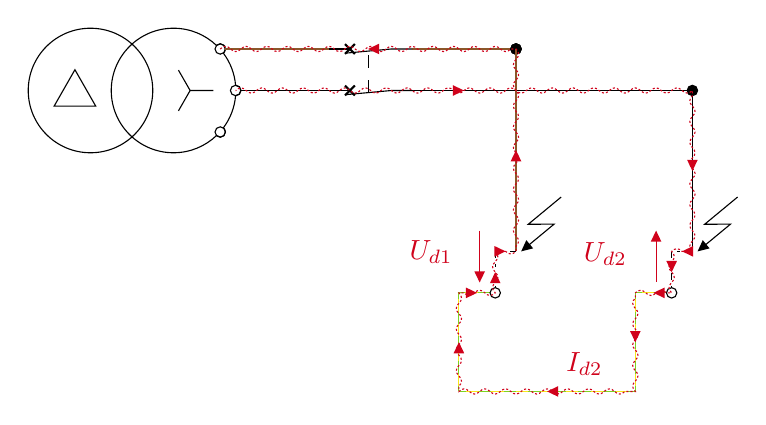
\begin{tikzpicture}[x=0.75pt,y=0.75pt,yscale=-1,xscale=1]
%uncomment if require: \path (0,219); %set diagram left start at 0, and has height of 219

%Straight Lines [id:da4511637283243949] 
\draw  [dash pattern={on 2.25pt off 2.25pt on 1pt off 2.25pt}]  (252.5,112.5) -- (242.5,112.5) -- (242.5,130) ;
%Straight Lines [id:da9527130819146642] 
\draw  [dash pattern={on 2.25pt off 2.25pt on 1pt off 2.25pt}]  (337.5,112.5) -- (327.5,112.5) -- (327.5,130) ;
%Straight Lines [id:da24126717784692808] 
\draw [color={rgb, 255:red, 0; green, 0; blue, 0 }  ,draw opacity=1 ]   (337.5,112.5) -- (337.5,35) ;
%Straight Lines [id:da3468467801372336] 
\draw    (202.5,35) -- (337.5,35) ;
%Straight Lines [id:da5563024891724297] 
\draw [color={rgb, 255:red, 139; green, 87; blue, 42 }  ,draw opacity=1 ]   (202.5,15) -- (252.5,15) ;
%Shape: Path Data [id:dp43837740322366014] 
\draw   (112.5,55) .. controls (112.5,56.38) and (111.38,57.5) .. (110,57.5) .. controls (109.29,57.5) and (108.65,57.2) .. (108.19,56.72) .. controls (102.81,61.85) and (95.52,65) .. (87.5,65) .. controls (70.93,65) and (57.5,51.57) .. (57.5,35) .. controls (57.5,18.43) and (70.93,5) .. (87.5,5) .. controls (95.52,5) and (102.81,8.15) .. (108.19,13.28) .. controls (108.65,12.8) and (109.29,12.5) .. (110,12.5) .. controls (111.38,12.5) and (112.5,13.62) .. (112.5,15) .. controls (112.5,15.82) and (112.11,16.54) .. (111.5,17) .. controls (114.8,21.39) and (116.92,26.71) .. (117.4,32.5) .. controls (117.43,32.5) and (117.47,32.5) .. (117.5,32.5) .. controls (118.88,32.5) and (120,33.62) .. (120,35) .. controls (120,36.38) and (118.88,37.5) .. (117.5,37.5) .. controls (117.47,37.5) and (117.43,37.5) .. (117.4,37.5) .. controls (116.92,43.29) and (114.8,48.61) .. (111.5,53) .. controls (112.11,53.46) and (112.5,54.18) .. (112.5,55) -- cycle ;
%Shape: Circle [id:dp03603482838008654] 
\draw   (17.5,35) .. controls (17.5,18.43) and (30.93,5) .. (47.5,5) .. controls (64.07,5) and (77.5,18.43) .. (77.5,35) .. controls (77.5,51.57) and (64.07,65) .. (47.5,65) .. controls (30.93,65) and (17.5,51.57) .. (17.5,35) -- cycle ;
%Shape: Triangle [id:dp7860018021593028] 
\draw   (40,25) -- (30,42.5) -- (50,42.5) -- cycle ;
%Shape: Star [id:dp36273195667205105] 
\draw   (106.75,35) -- (95.5,35) -- (89.88,44.81) -- (95.5,35) -- (89.88,25.19) -- (95.5,35) -- cycle ;
%Shape: Circle [id:dp581329576165861] 
\draw   (107.5,15) .. controls (107.5,13.62) and (108.62,12.5) .. (110,12.5) .. controls (111.38,12.5) and (112.5,13.62) .. (112.5,15) .. controls (112.5,16.38) and (111.38,17.5) .. (110,17.5) .. controls (108.62,17.5) and (107.5,16.38) .. (107.5,15) -- cycle ;
%Shape: Circle [id:dp008181652335233047] 
\draw   (114.9,35) .. controls (114.9,33.62) and (116.02,32.5) .. (117.4,32.5) .. controls (118.78,32.5) and (119.9,33.62) .. (119.9,35) .. controls (119.9,36.38) and (118.78,37.5) .. (117.4,37.5) .. controls (116.02,37.5) and (114.9,36.38) .. (114.9,35) -- cycle ;
%Shape: Circle [id:dp5428967410526352] 
\draw   (107.5,55) .. controls (107.5,53.62) and (108.62,52.5) .. (110,52.5) .. controls (111.38,52.5) and (112.5,53.62) .. (112.5,55) .. controls (112.5,56.38) and (111.38,57.5) .. (110,57.5) .. controls (108.62,57.5) and (107.5,56.38) .. (107.5,55) -- cycle ;

%Shape: Circle [id:dp3004196596154465] 
\draw  [fill={rgb, 255:red, 0; green, 0; blue, 0 }  ,fill opacity=1 ] (335,35) .. controls (335,33.62) and (336.12,32.5) .. (337.5,32.5) .. controls (338.88,32.5) and (340,33.62) .. (340,35) .. controls (340,36.38) and (338.88,37.5) .. (337.5,37.5) .. controls (336.12,37.5) and (335,36.38) .. (335,35) -- cycle ;
%Shape: Circle [id:dp38478162693673257] 
\draw  [fill={rgb, 255:red, 0; green, 0; blue, 0 }  ,fill opacity=1 ] (250,15) .. controls (250,13.62) and (251.12,12.5) .. (252.5,12.5) .. controls (253.88,12.5) and (255,13.62) .. (255,15) .. controls (255,16.38) and (253.88,17.5) .. (252.5,17.5) .. controls (251.12,17.5) and (250,16.38) .. (250,15) -- cycle ;
%Straight Lines [id:da35747201510733806] 
\draw [color={rgb, 255:red, 139; green, 87; blue, 42 }  ,draw opacity=1 ]   (112.5,15) -- (162.5,15) ;
%Straight Lines [id:da03938247690059582] 
\draw    (120,35) -- (162.5,35) ;
%Shape: Boxed Line [id:dp47312336425022783] 
\draw    (274.27,86.33) -- (258.39,99.47) -- (270.89,99.36) -- (257.31,110.59) ;
\draw [shift={(255,112.5)}, rotate = 320.40999999999997] [fill={rgb, 255:red, 0; green, 0; blue, 0 }  ][line width=0.08]  [draw opacity=0] (5.36,-2.57) -- (0,0) -- (5.36,2.57) -- cycle    ;
%Shape: Boxed Line [id:dp8604246706425941] 
\draw    (359.27,86.33) -- (343.39,99.47) -- (355.89,99.36) -- (342.31,110.59) ;
\draw [shift={(340,112.5)}, rotate = 320.40999999999997] [fill={rgb, 255:red, 0; green, 0; blue, 0 }  ][line width=0.08]  [draw opacity=0] (5.36,-2.57) -- (0,0) -- (5.36,2.57) -- cycle    ;
%Straight Lines [id:da6306782474143875] 
\draw    (170.5,37) -- (192.5,35) -- (202.5,35) ;
%Straight Lines [id:da4629224352649184] 
\draw    (172.5,35) -- (162.5,35) ;
\draw [shift={(172.5,35)}, rotate = 225] [color={rgb, 255:red, 0; green, 0; blue, 0 }  ][line width=0.75]    (-3.35,0) -- (3.35,0)(0,3.35) -- (0,-3.35)   ;
%Straight Lines [id:da5132783320552895] 
\draw    (170.5,17) -- (192.5,15) -- (202.5,15) ;
%Straight Lines [id:da123841191189479] 
\draw  [dash pattern={on 4.5pt off 4.5pt}]  (181.5,36) -- (181.5,16) ;
%Straight Lines [id:da38134434479229706] 
\draw    (172.5,15) -- (162.5,15) ;
\draw [shift={(172.5,15)}, rotate = 225] [color={rgb, 255:red, 0; green, 0; blue, 0 }  ][line width=0.75]    (-3.35,0) -- (3.35,0)(0,3.35) -- (0,-3.35)   ;

%Straight Lines [id:da029862379270012007] 
\draw [color={rgb, 255:red, 139; green, 87; blue, 42 }  ,draw opacity=1 ]   (252.5,112.5) -- (252.5,15) ;
%Shape: Circle [id:dp10157043967465573] 
\draw  [fill={rgb, 255:red, 0; green, 0; blue, 0 }  ,fill opacity=1 ] (250,15) .. controls (250,13.62) and (251.12,12.5) .. (252.5,12.5) .. controls (253.88,12.5) and (255,13.62) .. (255,15) .. controls (255,16.38) and (253.88,17.5) .. (252.5,17.5) .. controls (251.12,17.5) and (250,16.38) .. (250,15) -- cycle ;
%Shape: Circle [id:dp8079725241460669] 
\draw  [fill={rgb, 255:red, 0; green, 0; blue, 0 }  ,fill opacity=1 ] (250,15) .. controls (250,13.62) and (251.12,12.5) .. (252.5,12.5) .. controls (253.88,12.5) and (255,13.62) .. (255,15) .. controls (255,16.38) and (253.88,17.5) .. (252.5,17.5) .. controls (251.12,17.5) and (250,16.38) .. (250,15) -- cycle ;
%Straight Lines [id:da32787816985288987] 
\draw [color={rgb, 255:red, 208; green, 2; blue, 27 }  ,draw opacity=1 ]   (235,102.5) -- (235,124.5) ;
\draw [shift={(235,127.5)}, rotate = 270] [fill={rgb, 255:red, 208; green, 2; blue, 27 }  ,fill opacity=1 ][line width=0.08]  [draw opacity=0] (5.36,-2.57) -- (0,0) -- (5.36,2.57) -- cycle    ;
%Straight Lines [id:da9290035127505091] 
\draw [color={rgb, 255:red, 208; green, 2; blue, 27 }  ,draw opacity=1 ]   (320,105.5) -- (320,127.5) ;
\draw [shift={(320,102.5)}, rotate = 90] [fill={rgb, 255:red, 208; green, 2; blue, 27 }  ,fill opacity=1 ][line width=0.08]  [draw opacity=0] (5.36,-2.57) -- (0,0) -- (5.36,2.57) -- cycle    ;
%Straight Lines [id:da4236883272393758] 
\draw [color={rgb, 255:red, 248; green, 231; blue, 28 }  ,draw opacity=1 ]   (325,132.5) -- (310,132.5) -- (310,180) -- (225,180) ;
%Straight Lines [id:da1955939853197214] 
\draw [color={rgb, 255:red, 126; green, 211; blue, 33 }  ,draw opacity=1 ] [dash pattern={on 4.5pt off 4.5pt}]  (325,132.5) -- (310,132.5) -- (310,180) -- (225,180) ;
%Straight Lines [id:da8052192234703028] 
\draw [color={rgb, 255:red, 248; green, 231; blue, 28 }  ,draw opacity=1 ]   (240,132.5) -- (225,132.5) -- (225,180) ;
%Straight Lines [id:da6976347779102222] 
\draw [color={rgb, 255:red, 139; green, 87; blue, 42 }  ,draw opacity=1 ]   (252.5,110) -- (252.5,15) ;
%Straight Lines [id:da2970008681971681] 
\draw [color={rgb, 255:red, 126; green, 211; blue, 33 }  ,draw opacity=1 ] [dash pattern={on 4.5pt off 4.5pt}]  (240,132.5) -- (225,132.5) -- (225,180) ;
%Straight Lines [id:da7142618830255841] 
\draw [color={rgb, 255:red, 0; green, 0; blue, 0 }  ,draw opacity=1 ]   (337.5,110) -- (337.5,32.5) ;
%Shape: Circle [id:dp970057374964288] 
\draw  [fill={rgb, 255:red, 255; green, 255; blue, 255 }  ,fill opacity=1 ] (240,132.5) .. controls (240,131.12) and (241.12,130) .. (242.5,130) .. controls (243.88,130) and (245,131.12) .. (245,132.5) .. controls (245,133.88) and (243.88,135) .. (242.5,135) .. controls (241.12,135) and (240,133.88) .. (240,132.5) -- cycle ;
%Shape: Circle [id:dp5285112483449262] 
\draw  [fill={rgb, 255:red, 255; green, 255; blue, 255 }  ,fill opacity=1 ] (325,132.5) .. controls (325,131.12) and (326.12,130) .. (327.5,130) .. controls (328.88,130) and (330,131.12) .. (330,132.5) .. controls (330,133.88) and (328.88,135) .. (327.5,135) .. controls (326.12,135) and (325,133.88) .. (325,132.5) -- cycle ;
%Straight Lines [id:da2635484251048684] 
\draw [color={rgb, 255:red, 208; green, 2; blue, 27 }  ,draw opacity=1 ] [dash pattern={on 0.75pt off 0.75pt}]  (110,15) .. controls (111.67,13.33) and (113.33,13.33) .. (115,15) .. controls (116.67,16.67) and (118.33,16.67) .. (120,15) .. controls (121.67,13.33) and (123.33,13.33) .. (125,15) .. controls (126.67,16.67) and (128.33,16.67) .. (130,15) .. controls (131.67,13.33) and (133.33,13.33) .. (135,15) .. controls (136.67,16.67) and (138.33,16.67) .. (140,15) .. controls (141.67,13.33) and (143.33,13.33) .. (145,15) .. controls (146.67,16.67) and (148.33,16.67) .. (150,15) .. controls (151.67,13.33) and (153.33,13.33) .. (155,15) .. controls (156.67,16.67) and (158.33,16.67) .. (160,15) .. controls (161.67,13.33) and (163.33,13.33) .. (165,15) .. controls (166.67,16.67) and (168.33,16.67) .. (170,15) .. controls (171.67,13.33) and (173.33,13.33) .. (175,15) .. controls (176.67,16.67) and (178.33,16.67) .. (180,15) .. controls (181.67,13.33) and (183.33,13.33) .. (185,15) .. controls (186.67,16.67) and (188.33,16.67) .. (190,15) .. controls (191.67,13.33) and (193.33,13.33) .. (195,15) .. controls (196.67,16.67) and (198.33,16.67) .. (200,15) .. controls (201.67,13.33) and (203.33,13.33) .. (205,15) .. controls (206.67,16.67) and (208.33,16.67) .. (210,15) .. controls (211.67,13.33) and (213.33,13.33) .. (215,15) .. controls (216.67,16.67) and (218.33,16.67) .. (220,15) .. controls (221.67,13.33) and (223.33,13.33) .. (225,15) .. controls (226.67,16.67) and (228.33,16.67) .. (230,15) .. controls (231.67,13.33) and (233.33,13.33) .. (235,15) .. controls (236.67,16.67) and (238.33,16.67) .. (240,15) .. controls (241.67,13.33) and (243.33,13.33) .. (245,15) .. controls (246.67,16.67) and (248.33,16.67) .. (250,15) -- (252.5,15) -- (252.5,15) .. controls (254.17,16.67) and (254.17,18.33) .. (252.5,20) .. controls (250.83,21.67) and (250.83,23.33) .. (252.5,25) .. controls (254.17,26.67) and (254.17,28.33) .. (252.5,30) .. controls (250.83,31.67) and (250.83,33.33) .. (252.5,35) .. controls (254.17,36.67) and (254.17,38.33) .. (252.5,40) .. controls (250.83,41.67) and (250.83,43.33) .. (252.5,45) .. controls (254.17,46.67) and (254.17,48.33) .. (252.5,50) .. controls (250.83,51.67) and (250.83,53.33) .. (252.5,55) .. controls (254.17,56.67) and (254.17,58.33) .. (252.5,60) .. controls (250.83,61.67) and (250.83,63.33) .. (252.5,65) .. controls (254.17,66.67) and (254.17,68.33) .. (252.5,70) .. controls (250.83,71.67) and (250.83,73.33) .. (252.5,75) .. controls (254.17,76.67) and (254.17,78.33) .. (252.5,80) .. controls (250.83,81.67) and (250.83,83.33) .. (252.5,85) .. controls (254.17,86.67) and (254.17,88.33) .. (252.5,90) .. controls (250.83,91.67) and (250.83,93.33) .. (252.5,95) .. controls (254.17,96.67) and (254.17,98.33) .. (252.5,100) .. controls (250.83,101.67) and (250.83,103.33) .. (252.5,105) .. controls (254.17,106.67) and (254.17,108.33) .. (252.5,110) -- (252.5,112.5) -- (252.5,112.5) .. controls (250.83,114.17) and (249.17,114.17) .. (247.5,112.5) -- (242.5,112.5) -- (242.5,112.5) .. controls (244.17,114.17) and (244.17,115.83) .. (242.5,117.5) .. controls (240.83,119.17) and (240.83,120.83) .. (242.5,122.5) .. controls (244.17,124.17) and (244.17,125.83) .. (242.5,127.5) .. controls (240.83,129.17) and (240.83,130.83) .. (242.5,132.5) -- (242.5,132.5) .. controls (240.83,134.17) and (239.17,134.17) .. (237.5,132.5) .. controls (235.83,130.83) and (234.17,130.83) .. (232.5,132.5) .. controls (230.83,134.17) and (229.17,134.17) .. (227.5,132.5) -- (225,132.5) -- (225,132.5) .. controls (226.67,134.17) and (226.67,135.83) .. (225,137.5) .. controls (223.33,139.17) and (223.33,140.83) .. (225,142.5) .. controls (226.67,144.17) and (226.67,145.83) .. (225,147.5) .. controls (223.33,149.17) and (223.33,150.83) .. (225,152.5) .. controls (226.67,154.17) and (226.67,155.83) .. (225,157.5) .. controls (223.33,159.17) and (223.33,160.83) .. (225,162.5) .. controls (226.67,164.17) and (226.67,165.83) .. (225,167.5) .. controls (223.33,169.17) and (223.33,170.83) .. (225,172.5) .. controls (226.67,174.17) and (226.67,175.83) .. (225,177.5) -- (225,180) -- (225,180) .. controls (226.67,178.33) and (228.33,178.33) .. (230,180) .. controls (231.67,181.67) and (233.33,181.67) .. (235,180) .. controls (236.67,178.33) and (238.33,178.33) .. (240,180) .. controls (241.67,181.67) and (243.33,181.67) .. (245,180) .. controls (246.67,178.33) and (248.33,178.33) .. (250,180) .. controls (251.67,181.67) and (253.33,181.67) .. (255,180) .. controls (256.67,178.33) and (258.33,178.33) .. (260,180) .. controls (261.67,181.67) and (263.33,181.67) .. (265,180) .. controls (266.67,178.33) and (268.33,178.33) .. (270,180) .. controls (271.67,181.67) and (273.33,181.67) .. (275,180) .. controls (276.67,178.33) and (278.33,178.33) .. (280,180) .. controls (281.67,181.67) and (283.33,181.67) .. (285,180) .. controls (286.67,178.33) and (288.33,178.33) .. (290,180) .. controls (291.67,181.67) and (293.33,181.67) .. (295,180) .. controls (296.67,178.33) and (298.33,178.33) .. (300,180) .. controls (301.67,181.67) and (303.33,181.67) .. (305,180) -- (310,180) -- (310,180) .. controls (308.33,178.33) and (308.33,176.67) .. (310,175) .. controls (311.67,173.33) and (311.67,171.67) .. (310,170) .. controls (308.33,168.33) and (308.33,166.67) .. (310,165) .. controls (311.67,163.33) and (311.67,161.67) .. (310,160) .. controls (308.33,158.33) and (308.33,156.67) .. (310,155) .. controls (311.67,153.33) and (311.67,151.67) .. (310,150) .. controls (308.33,148.33) and (308.33,146.67) .. (310,145) .. controls (311.67,143.33) and (311.67,141.67) .. (310,140) .. controls (308.33,138.33) and (308.33,136.67) .. (310,135) -- (310,132.5) -- (310,132.5) .. controls (311.67,130.83) and (313.33,130.83) .. (315,132.5) .. controls (316.67,134.17) and (318.33,134.17) .. (320,132.5) .. controls (321.67,130.83) and (323.33,130.83) .. (325,132.5) -- (327.5,132.5) -- (327.5,132.5) .. controls (325.83,130.83) and (325.83,129.17) .. (327.5,127.5) .. controls (329.17,125.83) and (329.17,124.17) .. (327.5,122.5) .. controls (325.83,120.83) and (325.83,119.17) .. (327.5,117.5) .. controls (329.17,115.83) and (329.17,114.17) .. (327.5,112.5) -- (327.5,112.5) .. controls (329.17,110.83) and (330.83,110.83) .. (332.5,112.5) -- (337.5,112.5) -- (337.5,112.5) .. controls (335.83,110.83) and (335.83,109.17) .. (337.5,107.5) .. controls (339.17,105.83) and (339.17,104.17) .. (337.5,102.5) .. controls (335.83,100.83) and (335.83,99.17) .. (337.5,97.5) .. controls (339.17,95.83) and (339.17,94.17) .. (337.5,92.5) .. controls (335.83,90.83) and (335.83,89.17) .. (337.5,87.5) .. controls (339.17,85.83) and (339.17,84.17) .. (337.5,82.5) .. controls (335.83,80.83) and (335.83,79.17) .. (337.5,77.5) .. controls (339.17,75.83) and (339.17,74.17) .. (337.5,72.5) .. controls (335.83,70.83) and (335.83,69.17) .. (337.5,67.5) .. controls (339.17,65.83) and (339.17,64.17) .. (337.5,62.5) .. controls (335.83,60.83) and (335.83,59.17) .. (337.5,57.5) .. controls (339.17,55.83) and (339.17,54.17) .. (337.5,52.5) .. controls (335.83,50.83) and (335.83,49.17) .. (337.5,47.5) .. controls (339.17,45.83) and (339.17,44.17) .. (337.5,42.5) .. controls (335.83,40.83) and (335.83,39.17) .. (337.5,37.5) -- (337.5,35) -- (337.5,35) .. controls (335.83,36.67) and (334.17,36.67) .. (332.5,35) .. controls (330.83,33.33) and (329.17,33.33) .. (327.5,35) .. controls (325.83,36.67) and (324.17,36.67) .. (322.5,35) .. controls (320.83,33.33) and (319.17,33.33) .. (317.5,35) .. controls (315.83,36.67) and (314.17,36.67) .. (312.5,35) .. controls (310.83,33.33) and (309.17,33.33) .. (307.5,35) .. controls (305.83,36.67) and (304.17,36.67) .. (302.5,35) .. controls (300.83,33.33) and (299.17,33.33) .. (297.5,35) .. controls (295.83,36.67) and (294.17,36.67) .. (292.5,35) .. controls (290.83,33.33) and (289.17,33.33) .. (287.5,35) .. controls (285.83,36.67) and (284.17,36.67) .. (282.5,35) .. controls (280.83,33.33) and (279.17,33.33) .. (277.5,35) .. controls (275.83,36.67) and (274.17,36.67) .. (272.5,35) .. controls (270.83,33.33) and (269.17,33.33) .. (267.5,35) .. controls (265.83,36.67) and (264.17,36.67) .. (262.5,35) .. controls (260.83,33.33) and (259.17,33.33) .. (257.5,35) .. controls (255.83,36.67) and (254.17,36.67) .. (252.5,35) .. controls (250.83,33.33) and (249.17,33.33) .. (247.5,35) .. controls (245.83,36.67) and (244.17,36.67) .. (242.5,35) .. controls (240.83,33.33) and (239.17,33.33) .. (237.5,35) .. controls (235.83,36.67) and (234.17,36.67) .. (232.5,35) .. controls (230.83,33.33) and (229.17,33.33) .. (227.5,35) .. controls (225.83,36.67) and (224.17,36.67) .. (222.5,35) .. controls (220.83,33.33) and (219.17,33.33) .. (217.5,35) .. controls (215.83,36.67) and (214.17,36.67) .. (212.5,35) .. controls (210.83,33.33) and (209.17,33.33) .. (207.5,35) .. controls (205.83,36.67) and (204.17,36.67) .. (202.5,35) .. controls (200.83,33.33) and (199.17,33.33) .. (197.5,35) .. controls (195.83,36.67) and (194.17,36.67) .. (192.5,35) .. controls (190.83,33.33) and (189.17,33.33) .. (187.5,35) .. controls (185.83,36.67) and (184.17,36.67) .. (182.5,35) .. controls (180.83,33.33) and (179.17,33.33) .. (177.5,35) .. controls (175.83,36.67) and (174.17,36.67) .. (172.5,35) .. controls (170.83,33.33) and (169.17,33.33) .. (167.5,35) .. controls (165.83,36.67) and (164.17,36.67) .. (162.5,35) .. controls (160.83,33.33) and (159.17,33.33) .. (157.5,35) .. controls (155.83,36.67) and (154.17,36.67) .. (152.5,35) .. controls (150.83,33.33) and (149.17,33.33) .. (147.5,35) .. controls (145.83,36.67) and (144.17,36.67) .. (142.5,35) .. controls (140.83,33.33) and (139.17,33.33) .. (137.5,35) .. controls (135.83,36.67) and (134.17,36.67) .. (132.5,35) .. controls (130.83,33.33) and (129.17,33.33) .. (127.5,35) .. controls (125.83,36.67) and (124.17,36.67) .. (122.5,35) .. controls (120.83,33.33) and (119.17,33.33) .. (117.5,35) -- (117.4,35) -- (117.4,35) ;
\draw [shift={(181.25,15)}, rotate = 0] [fill={rgb, 255:red, 208; green, 2; blue, 27 }  ,fill opacity=1 ][line width=0.08]  [draw opacity=0] (5.36,-2.57) -- (0,0) -- (5.36,2.57) -- cycle    ;
\draw [shift={(252.5,63.75)}, rotate = 90] [fill={rgb, 255:red, 208; green, 2; blue, 27 }  ,fill opacity=1 ][line width=0.08]  [draw opacity=0] (5.36,-2.57) -- (0,0) -- (5.36,2.57) -- cycle    ;
\draw [shift={(247.5,112.5)}, rotate = 180] [fill={rgb, 255:red, 208; green, 2; blue, 27 }  ,fill opacity=1 ][line width=0.08]  [draw opacity=0] (5.36,-2.57) -- (0,0) -- (5.36,2.57) -- cycle    ;
\draw [shift={(242.5,122.5)}, rotate = 90] [fill={rgb, 255:red, 208; green, 2; blue, 27 }  ,fill opacity=1 ][line width=0.08]  [draw opacity=0] (5.36,-2.57) -- (0,0) -- (5.36,2.57) -- cycle    ;
\draw [shift={(233.75,132.5)}, rotate = 180] [fill={rgb, 255:red, 208; green, 2; blue, 27 }  ,fill opacity=1 ][line width=0.08]  [draw opacity=0] (5.36,-2.57) -- (0,0) -- (5.36,2.57) -- cycle    ;
\draw [shift={(225,156.25)}, rotate = 90] [fill={rgb, 255:red, 208; green, 2; blue, 27 }  ,fill opacity=1 ][line width=0.08]  [draw opacity=0] (5.36,-2.57) -- (0,0) -- (5.36,2.57) -- cycle    ;
\draw [shift={(267.5,180)}, rotate = 0] [fill={rgb, 255:red, 208; green, 2; blue, 27 }  ,fill opacity=1 ][line width=0.08]  [draw opacity=0] (5.36,-2.57) -- (0,0) -- (5.36,2.57) -- cycle    ;
\draw [shift={(310,156.25)}, rotate = 270] [fill={rgb, 255:red, 208; green, 2; blue, 27 }  ,fill opacity=1 ][line width=0.08]  [draw opacity=0] (5.36,-2.57) -- (0,0) -- (5.36,2.57) -- cycle    ;
\draw [shift={(318.75,132.5)}, rotate = 0] [fill={rgb, 255:red, 208; green, 2; blue, 27 }  ,fill opacity=1 ][line width=0.08]  [draw opacity=0] (5.36,-2.57) -- (0,0) -- (5.36,2.57) -- cycle    ;
\draw [shift={(327.5,122.5)}, rotate = 270] [fill={rgb, 255:red, 208; green, 2; blue, 27 }  ,fill opacity=1 ][line width=0.08]  [draw opacity=0] (5.36,-2.57) -- (0,0) -- (5.36,2.57) -- cycle    ;
\draw [shift={(332.5,112.5)}, rotate = 0] [fill={rgb, 255:red, 208; green, 2; blue, 27 }  ,fill opacity=1 ][line width=0.08]  [draw opacity=0] (5.36,-2.57) -- (0,0) -- (5.36,2.57) -- cycle    ;
\draw [shift={(337.5,73.75)}, rotate = 270] [fill={rgb, 255:red, 208; green, 2; blue, 27 }  ,fill opacity=1 ][line width=0.08]  [draw opacity=0] (5.36,-2.57) -- (0,0) -- (5.36,2.57) -- cycle    ;
\draw [shift={(227.45,35)}, rotate = 180] [fill={rgb, 255:red, 208; green, 2; blue, 27 }  ,fill opacity=1 ][line width=0.08]  [draw opacity=0] (5.36,-2.57) -- (0,0) -- (5.36,2.57) -- cycle    ;


% Text Node
\draw (275.5,160) node [anchor=north west][inner sep=0.75pt]  [color={rgb, 255:red, 208; green, 2; blue, 27 }  ,opacity=1 ] [align=left] {$I_{d2}$};
% Text Node
\draw (200,106) node [anchor=north west][inner sep=0.75pt]  [color={rgb, 255:red, 208; green, 2; blue, 27 }  ,opacity=1 ] [align=left] {$U_{d1}$};
% Text Node
\draw (284,107) node [anchor=north west][inner sep=0.75pt]  [color={rgb, 255:red, 208; green, 2; blue, 27 }  ,opacity=1 ] [align=left] {$U_{d2}$};


\end{tikzpicture}


\end{figure}

%\end{document}


L'intensité de courant $I_{d2}$ vaut alors :
\begin{formule}{Courant du deuxième défaut $I_{d2}$ en schéma Isolé-Interconnecté}{}
\begin{align*}
		I_{d2} &= \frac{0,5 \times U}{R_{ph1}+R_{ph2}} \\
\end{align*}

\begin{textvariables}
U								& tension nominale composée				& volt			& \volt					& 	Différence de potentiel entre deux conducteurs actifs (à préciser s'il s'agit du conducteur neutre)	\\
R_{ph1}					& résistance											& ohm			& \ohm					& 	Résistance de du conducteur actif alimentant l'appareil 1\\
R_{ph2}					& résistance											& ohm			& \ohm					& 	Résistance de du conducteur actif alimentant l'appareil 2\\
\end{textvariables}
\end{formule}

Le courant de défaut $I_{d1}$ fera alors apparaître une \emph{tension de défaut} $U_{d}$ entre la masse métallique de l'appareil 1 et la masse métallique de l'appareil 2. \\
On néglige également la résistance du conducteur PE devant celle des phases. Dans ce contexte-là, la tension de défaut $U_d$ vaut alors :

\begin{formule}{Tension de défaut $U_{d}$ en schéma Isolé-Individuel}{}
\begin{align*}
		U_{d} &= \frac{0,5 \times U}{2} \\
\end{align*}

\begin{textvariables}
U								& tension nominale composée				& volt			& \volt					& 	Différence de potentiel entre deux conducteurs actifs (à préciser s'il s'agit du conducteur neutre)	\\
I_{d2}						& intensité												& ampère		& \ampere				& 	Courant de défaut de l'appareil 2 \\
U_{L}						& tension							& volt			& \volt										& 	Tension de sécurité du local avec :
\begin{description}[nosep, leftmargin=*]
\item[Local sec :] $U_{L}=\SI{50}{\volt}$
\item[Local humide :] $U_{L}=\SI{25}{\volt}$
\end{description} \\
\end{textvariables}
\end{formule}

Cette tension de défaut est dangereuse et il faut obligatoirement couper l'alimentation en protégeant les circuits par des disjoncteurs magnéto-thermiques, qui doivent respecter les temps de coupure suivants :

%--------------------------------------
%ELECTROTECHNIQUE - SCHEMA DE LIAISON A LA TERRE
%--------------------------------------

%utiliser les environnement \begin{comment} \end{comment} pour mettre en commentaire le préambule une fois la programmation appelée dans le document maître (!ne pas oublier de mettre en commentaire \end{document}!)

\begin{comment}

\documentclass[a4paper, 11pt, twoside, fleqn]{memoir}

\usepackage{AOCDTF}

\marqueurchapitre
\decoupagechapitre{1} %juste pour éviter les erreurs lors de la compilation des sous-programmations (passera en commentaire)

%lien d'édition des figures Tikz sur le site mathcha.io (rajouter le lien d'une modification effectuée sur la figure tikz avec le nom du modificateur car il n'y a qu'un lien par compte)

%lien éditeur Bruno Douchy : https://www.mathcha.io/editor/zjygnFElSdyhJ72e3zT5ZgqwBT4DKnovswpXn1q

%--------------------------------------
%corps du document
%--------------------------------------

\begin{document} %corps du document
	\openleft %début de chapitre à gauche

\end{comment}

\begin{table}[H]
\caption{Temps de coupure maximal des disjoncteurs en schéma IT\label{tab:schema_it_temps_coupure}}
\begin{threeparttable} %note dans tableau
\begin{tabularx}{\textwidth}{C C C}
\toprule
\multirow[c]{2}{*}{\thead{Réseaux usuels}} & \multicolumn{2}{c}{\thead{Temps de coupure maximal (\si{\milli\second})}}\\
\cmidrule(lr){2-3} 
	& $U_{L}=\SI{50}{\volt}$ 	& 			$U_{L}=\SI{25}{\volt}$  \\
\midrule
\multicolumn{3}{l}{Neutre non distribué} \\
\middashrule
\SI{127}{\volt}/\SI{230}{\volt}		& 800		& 400 \\
\SI{230}{\volt}/\SI{400}{\volt}		& 400		& 200 \\
\SI{400}{\volt}/\SI{690}{\volt}		& 200		& 60 \\
\SI{690}{\volt}/\SI{1000}{\volt}	& 100		& 20 \\
\addlinespace
\multicolumn{3}{l}{Neutre distribué\tnote{1}} \\
\middashrule
\SI{127}{\volt}/\SI{230}{\volt}		& 5000		& 1000 \\
\SI{230}{\volt}/\SI{400}{\volt}		& 800		& 500 \\
\SI{400}{\volt}/\SI{690}{\volt}		& 400		& 200 \\
\SI{690}{\volt}/\SI{1000}{\volt}	& 200		& 80 \\
\bottomrule 
\end{tabularx}
\begin{tablenotes}
    \item[1] les installations monophasées sont considérées comme des installations à neutre distribué.
\end{tablenotes}
\end{threeparttable} %note dans tableau
\end{table}

%\end{document}



La longueur maximale des conducteurs en schéma IT avec les masses interconnectées se calcule avec les mêmes méthodes que pour les installations en schéma TN (voir \superref{sec:schema_tn_methode_conventionnelle}).

\section{Contrôle permanent de l'installation en schéma IT}

Quand l'installation électrique est en schéma IT, il est nécessaire d'avoir une équipe de maintenance à disposition pour intervenir rapidement en cas de premier défaut. Pour les détecter au plus vite, il faut installer un Contrôleur Permanent d'Isolement (CPI). Il s'agit d'un appareil placé en dérivation qui va calculer en permanence deux paramètres de l'installation :
\begin{description}
\item[\Circled{1} niveau d'isolement général $Z_{res}$ :] injection d'une tension (continue ou alternative de basse fréquence) entre le neutre et la terre, générant un \emph{courant de fuite} $I_f$ dont l'intensité sera proportionnellement inverse au niveau d'isolement général de l'installation électrique. Au-dessous d'un certain seuil d'isolement réglable (généralement entre \numrange{0,7}{100}\si{\kilo\ohm}), le CPI déclenche une alarme. 
\item[\Circled{2} apparition d'un défaut franc sur un circuit :] installation de tores de détection sur les circuits à surveiller, calculant la différence entre le courant entre et sortant (mécanisme similaire à ceux des DDR). Cela permet de localiser précisément les circuits en défaut.
\end{description} 

 \begin{figure}[H]
\caption{Installation Isolé-Individuelle avec CPI}
\begin{subfigure}[t]{0.49\linewidth}
%--------------------------------------
%ELECTROTECHNIQUE - SCHEMA DE LIAISON A LA TERRE
%--------------------------------------

%utiliser les environnement \begin{comment} \end{comment} pour mettre en commentaire le préambule une fois la programmation appelée dans le document maître (!ne pas oublier de mettre en commentaire \end{document}!)

\begin{comment}

\documentclass[a4paper, 11pt, twoside, fleqn]{memoir}

\usepackage{AOCDTF}

\marqueurchapitre
\decoupagechapitre{1} %juste pour éviter les erreurs lors de la compilation des sous-programmations (passera en commentaire)

%lien d'édition des figures Tikz sur le site mathcha.io (rajouter le lien d'une modification effectuée sur la figure tikz avec le nom du modificateur car il n'y a qu'un lien par compte)

%lien mathcha Bruno Douchy : https://www.mathcha.io/editor/jQKLoCODsYQuv6lo9wh5LQq3pSzO0mydSnpzwBy

%--------------------------------------
%corps du document
%--------------------------------------

\begin{document} %corps du document
	\openleft %début de chapitre à gauche

\end{comment}



% Pattern Info
 
\tikzset{
pattern size/.store in=\mcSize, 
pattern size = 5pt,
pattern thickness/.store in=\mcThickness, 
pattern thickness = 0.3pt,
pattern radius/.store in=\mcRadius, 
pattern radius = 1pt}
\makeatletter
\pgfutil@ifundefined{pgf@pattern@name@_2ybrnrdqo}{
\pgfdeclarepatternformonly[\mcThickness,\mcSize]{_2ybrnrdqo}
{\pgfqpoint{0pt}{0pt}}
{\pgfpoint{\mcSize+\mcThickness}{\mcSize+\mcThickness}}
{\pgfpoint{\mcSize}{\mcSize}}
{
\pgfsetcolor{\tikz@pattern@color}
\pgfsetlinewidth{\mcThickness}
\pgfpathmoveto{\pgfqpoint{0pt}{0pt}}
\pgfpathlineto{\pgfpoint{\mcSize+\mcThickness}{\mcSize+\mcThickness}}
\pgfusepath{stroke}
}}
\makeatother
\tikzset{every picture/.style={line width=0.5pt}} %set default line width to 0.75pt        

\begin{tikzpicture}[x=0.75pt,y=0.75pt,yscale=-0.6,xscale=0.6]
%uncomment if require: \path (0,320); %set diagram left start at 0, and has height of 320

%Straight Lines [id:da4922757986185987] 
\draw [color={rgb, 255:red, 74; green, 144; blue, 226 }  ,draw opacity=1 ]   (152.5,75) -- (162.5,75) ;
%Straight Lines [id:da4038713220143262] 
\draw [color={rgb, 255:red, 74; green, 144; blue, 226 }  ,draw opacity=1 ]   (462.5,175) -- (462.5,155) ;
%Straight Lines [id:da9166454765790462] 
\draw [color={rgb, 255:red, 74; green, 144; blue, 226 }  ,draw opacity=1 ]   (462.5,107.5) -- (462.5,77.5) ;
%Straight Lines [id:da9023577986083069] 
\draw [color={rgb, 255:red, 74; green, 144; blue, 226 }  ,draw opacity=1 ]   (377.5,175) -- (377.5,155) ;
%Straight Lines [id:da5928803977736146] 
\draw [color={rgb, 255:red, 74; green, 144; blue, 226 }  ,draw opacity=1 ]   (377.5,107.5) -- (377.5,77.5) ;
%Straight Lines [id:da30570583399348505] 
\draw [color={rgb, 255:red, 74; green, 144; blue, 226 }  ,draw opacity=1 ]   (292.5,175) -- (292.5,155) ;
%Straight Lines [id:da8819404575351564] 
\draw [color={rgb, 255:red, 139; green, 87; blue, 42 }  ,draw opacity=1 ]   (252.5,175) -- (252.5,155) ;
%Straight Lines [id:da28367841763640167] 
\draw [color={rgb, 255:red, 155; green, 155; blue, 155 }  ,draw opacity=1 ]   (422.5,175) -- (422.5,155) ;
%Straight Lines [id:da6880263813112385] 
\draw [color={rgb, 255:red, 0; green, 0; blue, 0 }  ,draw opacity=1 ]   (337.5,175) -- (337.5,152.5) ;
%Straight Lines [id:da8972215794381513] 
\draw [color={rgb, 255:red, 248; green, 231; blue, 28 }  ,draw opacity=1 ]   (87.5,75) -- (27.5,75) -- (27.5,182.5) ;
%Straight Lines [id:da07998178544200962] 
\draw [color={rgb, 255:red, 248; green, 231; blue, 28 }  ,draw opacity=1 ]   (95.5,35) -- (87.5,75) -- (87.5,107.5) ;
%Straight Lines [id:da7929766229120194] 
\draw [color={rgb, 255:red, 126; green, 211; blue, 33 }  ,draw opacity=1 ] [dash pattern={on 2.25pt off 2.25pt}]  (95.5,35) -- (87.5,75) -- (87.5,107.5) ;
%Straight Lines [id:da4949912109010227] 
\draw [color={rgb, 255:red, 74; green, 144; blue, 226 }  ,draw opacity=1 ]   (202.5,75) -- (460,75) ;
%Straight Lines [id:da7560950775201385] 
\draw [color={rgb, 255:red, 248; green, 231; blue, 28 }  ,draw opacity=1 ]   (240,180) -- (225,180) -- (225,182.5) ;
%Straight Lines [id:da49944531942669546] 
\draw    (202.5,35) -- (462.5,35) ;
%Straight Lines [id:da47196191445949953] 
\draw [color={rgb, 255:red, 139; green, 87; blue, 42 }  ,draw opacity=1 ]   (202.5,15) -- (462.5,15) ;
%Straight Lines [id:da034038054075003044] 
\draw [color={rgb, 255:red, 155; green, 155; blue, 155 }  ,draw opacity=1 ]   (202.5,55) -- (462.5,55) ;
%Shape: Path Data [id:dp09879682351014718] 
\draw   (112.5,55) .. controls (112.5,56.38) and (111.38,57.5) .. (110,57.5) .. controls (109.29,57.5) and (108.65,57.2) .. (108.19,56.72) .. controls (102.81,61.85) and (95.52,65) .. (87.5,65) .. controls (70.93,65) and (57.5,51.57) .. (57.5,35) .. controls (57.5,18.43) and (70.93,5) .. (87.5,5) .. controls (95.52,5) and (102.81,8.15) .. (108.19,13.28) .. controls (108.65,12.8) and (109.29,12.5) .. (110,12.5) .. controls (111.38,12.5) and (112.5,13.62) .. (112.5,15) .. controls (112.5,15.82) and (112.11,16.54) .. (111.5,17) .. controls (114.8,21.39) and (116.92,26.71) .. (117.4,32.5) .. controls (117.43,32.5) and (117.47,32.5) .. (117.5,32.5) .. controls (118.88,32.5) and (120,33.62) .. (120,35) .. controls (120,36.38) and (118.88,37.5) .. (117.5,37.5) .. controls (117.47,37.5) and (117.43,37.5) .. (117.4,37.5) .. controls (116.92,43.29) and (114.8,48.61) .. (111.5,53) .. controls (112.11,53.46) and (112.5,54.18) .. (112.5,55) -- cycle ;
%Shape: Circle [id:dp09395491014356527] 
\draw   (17.5,35) .. controls (17.5,18.43) and (30.93,5) .. (47.5,5) .. controls (64.07,5) and (77.5,18.43) .. (77.5,35) .. controls (77.5,51.57) and (64.07,65) .. (47.5,65) .. controls (30.93,65) and (17.5,51.57) .. (17.5,35) -- cycle ;
%Shape: Triangle [id:dp01558250765431457] 
\draw   (40,25) -- (30,42.5) -- (50,42.5) -- cycle ;
%Shape: Star [id:dp0013707252732991781] 
\draw   (106.75,35) -- (95.5,35) -- (89.88,44.81) -- (95.5,35) -- (89.88,25.19) -- (95.5,35) -- cycle ;
%Shape: Circle [id:dp39893592802184263] 
\draw   (107.5,15) .. controls (107.5,13.62) and (108.62,12.5) .. (110,12.5) .. controls (111.38,12.5) and (112.5,13.62) .. (112.5,15) .. controls (112.5,16.38) and (111.38,17.5) .. (110,17.5) .. controls (108.62,17.5) and (107.5,16.38) .. (107.5,15) -- cycle ;
%Shape: Circle [id:dp9893284041115082] 
\draw   (114.9,35) .. controls (114.9,33.62) and (116.02,32.5) .. (117.4,32.5) .. controls (118.78,32.5) and (119.9,33.62) .. (119.9,35) .. controls (119.9,36.38) and (118.78,37.5) .. (117.4,37.5) .. controls (116.02,37.5) and (114.9,36.38) .. (114.9,35) -- cycle ;
%Shape: Circle [id:dp3917292266620266] 
\draw   (107.5,55) .. controls (107.5,53.62) and (108.62,52.5) .. (110,52.5) .. controls (111.38,52.5) and (112.5,53.62) .. (112.5,55) .. controls (112.5,56.38) and (111.38,57.5) .. (110,57.5) .. controls (108.62,57.5) and (107.5,56.38) .. (107.5,55) -- cycle ;

%Straight Lines [id:da8322026187642189] 
\draw [color={rgb, 255:red, 139; green, 87; blue, 42 }  ,draw opacity=1 ]   (252.5,107.5) -- (252.5,15) ;
%Straight Lines [id:da8041249564118628] 
\draw [color={rgb, 255:red, 74; green, 144; blue, 226 }  ,draw opacity=1 ]   (292.5,107.5) -- (292.5,77.5) ;
%Straight Lines [id:da6342365727576158] 
\draw    (17.5,232.5) -- (460,232.5) ;
%Shape: Rectangle [id:dp8835182839666373] 
\draw  [draw opacity=0][pattern=_2ybrnrdqo,pattern size=6pt,pattern thickness=0.75pt,pattern radius=0pt, pattern color={rgb, 255:red, 0; green, 0; blue, 0}][line width=0.75]  (17.5,232.5) -- (460,232.5) -- (460,247.5) -- (17.5,247.5) -- cycle ;
%Straight Lines [id:da658767187431958] 
\draw [color={rgb, 255:red, 126; green, 211; blue, 33 }  ,draw opacity=1 ] [dash pattern={on 2.25pt off 2.25pt}]  (240,180) -- (225,180) -- (225,182.5) ;
%Straight Lines [id:da06637251377195108] 
\draw [color={rgb, 255:red, 248; green, 231; blue, 28 }  ,draw opacity=1 ]   (225,222.5) -- (225,247.5) ;
%Straight Lines [id:da47233881321451787] 
\draw    (225,247.5) -- (225,262.5) ;
%Straight Lines [id:da5035312706678949] 
\draw    (215,262.5) -- (235,262.5) ;
%Straight Lines [id:da18116556144696694] 
\draw    (217.5,267.5) -- (232.5,267.5) ;
%Straight Lines [id:da26663321343914415] 
\draw    (220,272.5) -- (230,272.5) ;

%Straight Lines [id:da7788639142047531] 
\draw [color={rgb, 255:red, 126; green, 211; blue, 33 }  ,draw opacity=1 ] [dash pattern={on 2.25pt off 2.25pt}]  (225,222.5) -- (225,247.5) ;
%Straight Lines [id:da8201802660928923] 
\draw    (287.5,175) -- (292.5,175) ;
%Shape: Rectangle [id:dp3438336194943209] 
\draw   (257.5,170) -- (287.5,170) -- (287.5,180) -- (257.5,180) -- cycle ;
%Straight Lines [id:da27605197781986657] 
\draw    (252.5,175) -- (257.5,175) ;

%Straight Lines [id:da9011697570747588] 
\draw    (225,217.5) -- (225,222.5) ;
%Shape: Rectangle [id:dp36989703847460553] 
\draw   (230,187.5) -- (230,217.5) -- (220,217.5) -- (220,187.5) -- cycle ;
%Straight Lines [id:da6366900985555619] 
\draw    (225,182.5) -- (225,187.5) ;

%Straight Lines [id:da3812281827541767] 
\draw [color={rgb, 255:red, 0; green, 0; blue, 0 }  ,draw opacity=1 ]   (337.5,107.5) -- (337.5,37.5) ;
%Straight Lines [id:da02888103671964104] 
\draw    (372.5,175) -- (377.5,175) ;
%Shape: Rectangle [id:dp39971735208919124] 
\draw   (342.5,170) -- (372.5,170) -- (372.5,180) -- (342.5,180) -- cycle ;
%Straight Lines [id:da15610963345624862] 
\draw    (337.5,175) -- (342.5,175) ;

%Straight Lines [id:da7566594469565104] 
\draw [color={rgb, 255:red, 155; green, 155; blue, 155 }  ,draw opacity=1 ]   (422.5,107.5) -- (422.5,57.5) ;
%Straight Lines [id:da9791907804470615] 
\draw [color={rgb, 255:red, 74; green, 144; blue, 226 }  ,draw opacity=1 ]   (462.5,175.5) -- (462.5,162.5) ;
%Straight Lines [id:da15543680976570695] 
\draw    (457.5,175) -- (462.5,175) ;
%Shape: Rectangle [id:dp27259637225024935] 
\draw   (427.5,170) -- (457.5,170) -- (457.5,180) -- (427.5,180) -- cycle ;
%Straight Lines [id:da6590266150100259] 
\draw    (422.5,175) -- (427.5,175) ;

%Shape: Circle [id:dp3040137945437842] 
\draw  [fill={rgb, 255:red, 0; green, 0; blue, 0 }  ,fill opacity=1 ] (375,75) .. controls (375,73.62) and (376.12,72.5) .. (377.5,72.5) .. controls (378.88,72.5) and (380,73.62) .. (380,75) .. controls (380,76.38) and (378.88,77.5) .. (377.5,77.5) .. controls (376.12,77.5) and (375,76.38) .. (375,75) -- cycle ;
%Shape: Circle [id:dp5886475323071111] 
\draw  [fill={rgb, 255:red, 0; green, 0; blue, 0 }  ,fill opacity=1 ] (460,75) .. controls (460,73.62) and (461.12,72.5) .. (462.5,72.5) .. controls (463.88,72.5) and (465,73.62) .. (465,75) .. controls (465,76.38) and (463.88,77.5) .. (462.5,77.5) .. controls (461.12,77.5) and (460,76.38) .. (460,75) -- cycle ;
%Shape: Circle [id:dp7341854734672731] 
\draw  [fill={rgb, 255:red, 0; green, 0; blue, 0 }  ,fill opacity=1 ] (335,35) .. controls (335,33.62) and (336.12,32.5) .. (337.5,32.5) .. controls (338.88,32.5) and (340,33.62) .. (340,35) .. controls (340,36.38) and (338.88,37.5) .. (337.5,37.5) .. controls (336.12,37.5) and (335,36.38) .. (335,35) -- cycle ;
%Shape: Circle [id:dp6336551833672776] 
\draw  [fill={rgb, 255:red, 0; green, 0; blue, 0 }  ,fill opacity=1 ] (420,55) .. controls (420,53.62) and (421.12,52.5) .. (422.5,52.5) .. controls (423.88,52.5) and (425,53.62) .. (425,55) .. controls (425,56.38) and (423.88,57.5) .. (422.5,57.5) .. controls (421.12,57.5) and (420,56.38) .. (420,55) -- cycle ;
%Shape: Circle [id:dp5716316243984012] 
\draw  [fill={rgb, 255:red, 0; green, 0; blue, 0 }  ,fill opacity=1 ] (290,75) .. controls (290,73.62) and (291.12,72.5) .. (292.5,72.5) .. controls (293.88,72.5) and (295,73.62) .. (295,75) .. controls (295,76.38) and (293.88,77.5) .. (292.5,77.5) .. controls (291.12,77.5) and (290,76.38) .. (290,75) -- cycle ;
%Shape: Circle [id:dp9134099794169516] 
\draw  [fill={rgb, 255:red, 0; green, 0; blue, 0 }  ,fill opacity=1 ] (250,15) .. controls (250,13.62) and (251.12,12.5) .. (252.5,12.5) .. controls (253.88,12.5) and (255,13.62) .. (255,15) .. controls (255,16.38) and (253.88,17.5) .. (252.5,17.5) .. controls (251.12,17.5) and (250,16.38) .. (250,15) -- cycle ;
%Shape: Rectangle [id:dp9736059741519228] 
\draw  [dash pattern={on 2.25pt off 2.25pt on 1pt off 2.25pt}] (242.5,160) -- (302.5,160) -- (302.5,190) -- (242.5,190) -- cycle ;
%Shape: Circle [id:dp314574850816974] 
\draw  [fill={rgb, 255:red, 255; green, 255; blue, 255 }  ,fill opacity=1 ] (240,180) .. controls (240,178.62) and (241.12,177.5) .. (242.5,177.5) .. controls (243.88,177.5) and (245,178.62) .. (245,180) .. controls (245,181.38) and (243.88,182.5) .. (242.5,182.5) .. controls (241.12,182.5) and (240,181.38) .. (240,180) -- cycle ;
%Shape: Circle [id:dp27575875918191606] 
\draw  [fill={rgb, 255:red, 255; green, 255; blue, 255 }  ,fill opacity=1 ] (250,160) .. controls (250,158.62) and (251.12,157.5) .. (252.5,157.5) .. controls (253.88,157.5) and (255,158.62) .. (255,160) .. controls (255,161.38) and (253.88,162.5) .. (252.5,162.5) .. controls (251.12,162.5) and (250,161.38) .. (250,160) -- cycle ;
%Shape: Circle [id:dp7954116399024105] 
\draw  [fill={rgb, 255:red, 255; green, 255; blue, 255 }  ,fill opacity=1 ] (290,160) .. controls (290,158.62) and (291.12,157.5) .. (292.5,157.5) .. controls (293.88,157.5) and (295,158.62) .. (295,160) .. controls (295,161.38) and (293.88,162.5) .. (292.5,162.5) .. controls (291.12,162.5) and (290,161.38) .. (290,160) -- cycle ;
%Shape: Rectangle [id:dp6541068284877478] 
\draw  [dash pattern={on 2.25pt off 2.25pt on 1pt off 2.25pt}] (327.5,160) -- (387.5,160) -- (387.5,190) -- (327.5,190) -- cycle ;
%Shape: Circle [id:dp018941541358536207] 
\draw  [fill={rgb, 255:red, 255; green, 255; blue, 255 }  ,fill opacity=1 ] (335,160) .. controls (335,158.62) and (336.12,157.5) .. (337.5,157.5) .. controls (338.88,157.5) and (340,158.62) .. (340,160) .. controls (340,161.38) and (338.88,162.5) .. (337.5,162.5) .. controls (336.12,162.5) and (335,161.38) .. (335,160) -- cycle ;
%Shape: Circle [id:dp6016021599386189] 
\draw  [fill={rgb, 255:red, 255; green, 255; blue, 255 }  ,fill opacity=1 ] (375,160) .. controls (375,158.62) and (376.12,157.5) .. (377.5,157.5) .. controls (378.88,157.5) and (380,158.62) .. (380,160) .. controls (380,161.38) and (378.88,162.5) .. (377.5,162.5) .. controls (376.12,162.5) and (375,161.38) .. (375,160) -- cycle ;
%Shape: Rectangle [id:dp28129735245298193] 
\draw  [dash pattern={on 2.25pt off 2.25pt on 1pt off 2.25pt}] (412.5,160) -- (472.5,160) -- (472.5,190) -- (412.5,190) -- cycle ;
%Shape: Circle [id:dp5457672494223385] 
\draw  [fill={rgb, 255:red, 255; green, 255; blue, 255 }  ,fill opacity=1 ] (420,160) .. controls (420,158.62) and (421.12,157.5) .. (422.5,157.5) .. controls (423.88,157.5) and (425,158.62) .. (425,160) .. controls (425,161.38) and (423.88,162.5) .. (422.5,162.5) .. controls (421.12,162.5) and (420,161.38) .. (420,160) -- cycle ;
%Shape: Circle [id:dp004736262340387043] 
\draw  [fill={rgb, 255:red, 255; green, 255; blue, 255 }  ,fill opacity=1 ] (460,160) .. controls (460,158.62) and (461.12,157.5) .. (462.5,157.5) .. controls (463.88,157.5) and (465,158.62) .. (465,160) .. controls (465,161.38) and (463.88,162.5) .. (462.5,162.5) .. controls (461.12,162.5) and (460,161.38) .. (460,160) -- cycle ;
%Straight Lines [id:da9415522099428929] 
\draw [color={rgb, 255:red, 139; green, 87; blue, 42 }  ,draw opacity=1 ]   (112.5,15) -- (162.5,15) ;
%Straight Lines [id:da42696925509974504] 
\draw [color={rgb, 255:red, 155; green, 155; blue, 155 }  ,draw opacity=1 ]   (112.5,55) -- (162.5,55) ;
%Straight Lines [id:da7637220357739247] 
\draw    (120,35) -- (162.5,35) ;
%Straight Lines [id:da38386833214397864] 
\draw    (87.5,217.5) -- (87.5,222.5) ;
%Shape: Rectangle [id:dp9683000231543459] 
\draw   (92.5,187.5) -- (92.5,217.5) -- (82.5,217.5) -- (82.5,187.5) -- cycle ;
%Straight Lines [id:da2704722512834088] 
\draw    (87.5,182.5) -- (87.5,187.5) ;

%Straight Lines [id:da2880234441278331] 
\draw [color={rgb, 255:red, 248; green, 231; blue, 28 }  ,draw opacity=1 ]   (87.5,222.5) -- (87.5,247.5) ;
%Straight Lines [id:da04608400213538033] 
\draw    (87.5,247.5) -- (87.5,262.5) ;
%Straight Lines [id:da41466559437331085] 
\draw    (77.5,262.5) -- (97.5,262.5) ;
%Straight Lines [id:da2626722205271087] 
\draw    (80,267.5) -- (95,267.5) ;
%Straight Lines [id:da21222747344424597] 
\draw    (82.5,272.5) -- (92.5,272.5) ;

%Straight Lines [id:da670095599036029] 
\draw [color={rgb, 255:red, 126; green, 211; blue, 33 }  ,draw opacity=1 ] [dash pattern={on 2.25pt off 2.25pt}]  (87.5,222.5) -- (87.5,247.5) ;
%Straight Lines [id:da02913653895526247] 
\draw [color={rgb, 255:red, 248; green, 231; blue, 28 }  ,draw opacity=1 ]   (325,180) -- (310,180) -- (310,182.5) ;
%Straight Lines [id:da4447650582892084] 
\draw [color={rgb, 255:red, 126; green, 211; blue, 33 }  ,draw opacity=1 ] [dash pattern={on 2.25pt off 2.25pt}]  (325,180) -- (310,180) -- (310,182.5) ;
%Straight Lines [id:da8975873804835947] 
\draw    (310,217.5) -- (310,222.5) ;
%Shape: Rectangle [id:dp046027364736950016] 
\draw   (315,187.5) -- (315,217.5) -- (305,217.5) -- (305,187.5) -- cycle ;
%Straight Lines [id:da8127198695850476] 
\draw    (310,182.5) -- (310,187.5) ;

%Shape: Circle [id:dp28495331318983497] 
\draw  [fill={rgb, 255:red, 255; green, 255; blue, 255 }  ,fill opacity=1 ] (325,180) .. controls (325,178.62) and (326.12,177.5) .. (327.5,177.5) .. controls (328.88,177.5) and (330,178.62) .. (330,180) .. controls (330,181.38) and (328.88,182.5) .. (327.5,182.5) .. controls (326.12,182.5) and (325,181.38) .. (325,180) -- cycle ;
%Straight Lines [id:da6784220288728289] 
\draw [color={rgb, 255:red, 248; green, 231; blue, 28 }  ,draw opacity=1 ]   (410,180) -- (395,180) -- (395,182.5) ;
%Straight Lines [id:da2905622575346154] 
\draw [color={rgb, 255:red, 126; green, 211; blue, 33 }  ,draw opacity=1 ] [dash pattern={on 2.25pt off 2.25pt}]  (410,180) -- (395,180) -- (395,182.5) ;
%Straight Lines [id:da5300169805654166] 
\draw    (395,217.5) -- (395,222.5) ;
%Shape: Rectangle [id:dp46954719074452567] 
\draw   (400,187.5) -- (400,217.5) -- (390,217.5) -- (390,187.5) -- cycle ;
%Straight Lines [id:da5294770126629791] 
\draw    (395,182.5) -- (395,187.5) ;

%Straight Lines [id:da6136211781243461] 
\draw [color={rgb, 255:red, 248; green, 231; blue, 28 }  ,draw opacity=1 ]   (310,222.5) -- (310,247.5) ;
%Straight Lines [id:da434872767407545] 
\draw    (310,247.5) -- (310,262.5) ;
%Straight Lines [id:da41166925954518063] 
\draw    (300,262.5) -- (320,262.5) ;
%Straight Lines [id:da756150701279873] 
\draw    (302.5,267.5) -- (317.5,267.5) ;
%Straight Lines [id:da43101095245627397] 
\draw    (305,272.5) -- (315,272.5) ;

%Straight Lines [id:da3718565783863639] 
\draw [color={rgb, 255:red, 126; green, 211; blue, 33 }  ,draw opacity=1 ] [dash pattern={on 2.25pt off 2.25pt}]  (310,222.5) -- (310,247.5) ;
%Straight Lines [id:da016815392155546505] 
\draw [color={rgb, 255:red, 248; green, 231; blue, 28 }  ,draw opacity=1 ]   (395,222.5) -- (395,247.5) ;
%Straight Lines [id:da8735181178492252] 
\draw    (395,247.5) -- (395,262.5) ;
%Straight Lines [id:da2459053119977932] 
\draw    (385,262.5) -- (405,262.5) ;
%Straight Lines [id:da04363419697670501] 
\draw    (387.5,267.5) -- (402.5,267.5) ;
%Straight Lines [id:da08890056887215114] 
\draw    (390,272.5) -- (400,272.5) ;

%Straight Lines [id:da9385371137486506] 
\draw [color={rgb, 255:red, 126; green, 211; blue, 33 }  ,draw opacity=1 ] [dash pattern={on 2.25pt off 2.25pt}]  (395,222.5) -- (395,247.5) ;
%Shape: Circle [id:dp4443919963813725] 
\draw  [fill={rgb, 255:red, 255; green, 255; blue, 255 }  ,fill opacity=1 ] (410,180) .. controls (410,178.62) and (411.12,177.5) .. (412.5,177.5) .. controls (413.88,177.5) and (415,178.62) .. (415,180) .. controls (415,181.38) and (413.88,182.5) .. (412.5,182.5) .. controls (411.12,182.5) and (410,181.38) .. (410,180) -- cycle ;
%Straight Lines [id:da12365146032326157] 
\draw [color={rgb, 255:red, 126; green, 211; blue, 33 }  ,draw opacity=1 ] [dash pattern={on 2.25pt off 2.25pt}]  (87.5,75) -- (27.5,75) -- (27.5,182.5) ;
%Straight Lines [id:da5074366501469295] 
\draw    (27.5,217.5) -- (27.5,222.5) ;
%Shape: Rectangle [id:dp3959830437796208] 
\draw   (32.5,187.5) -- (32.5,217.5) -- (22.5,217.5) -- (22.5,187.5) -- cycle ;
%Straight Lines [id:da351944066588591] 
\draw    (27.5,182.5) -- (27.5,187.5) ;

%Straight Lines [id:da4882348960061499] 
\draw [color={rgb, 255:red, 248; green, 231; blue, 28 }  ,draw opacity=1 ]   (27.5,222.5) -- (27.5,247.5) ;
%Straight Lines [id:da3290703017288258] 
\draw [color={rgb, 255:red, 126; green, 211; blue, 33 }  ,draw opacity=1 ] [dash pattern={on 2.25pt off 2.25pt}]  (27.5,222.5) -- (27.5,247.5) ;
%Straight Lines [id:da12861224423084006] 
\draw    (27.5,247.5) -- (27.5,262.5) ;
%Straight Lines [id:da6386518706593862] 
\draw    (17.5,262.5) -- (37.5,262.5) ;
%Straight Lines [id:da18415307770918254] 
\draw    (20,267.5) -- (35,267.5) ;
%Straight Lines [id:da35760082633081036] 
\draw    (22.5,272.5) -- (32.5,272.5) ;

%Straight Lines [id:da5529647452215599] 
\draw    (87.5,107.5) -- (87.5,132) ;
\draw [shift={(87.5,135)}, rotate = 270] [fill={rgb, 255:red, 0; green, 0; blue, 0 }  ][line width=0.08]  [draw opacity=0] (5.36,-2.57) -- (0,0) -- (5.36,2.57) -- cycle    ;
%Straight Lines [id:da15999437574266406] 
\draw    (87.5,167.5) -- (87.5,143) ;
\draw [shift={(87.5,140)}, rotate = 450] [fill={rgb, 255:red, 0; green, 0; blue, 0 }  ][line width=0.08]  [draw opacity=0] (5.36,-2.57) -- (0,0) -- (5.36,2.57) -- cycle    ;

%Straight Lines [id:da0047474836324150615] 
\draw [color={rgb, 255:red, 248; green, 231; blue, 28 }  ,draw opacity=1 ]   (87.5,167.5) -- (87.5,182.5) ;
%Straight Lines [id:da6984740545694063] 
\draw [color={rgb, 255:red, 126; green, 211; blue, 33 }  ,draw opacity=1 ] [dash pattern={on 2.25pt off 2.25pt}]  (87.5,167.5) -- (87.5,182.5) ;
%Shape: Boxed Line [id:dp5442036861143354] 
\draw    (223.23,141.57) -- (236.87,157.03) -- (236.36,144.54) -- (248.02,157.75) ;
\draw [shift={(250,160)}, rotate = 228.57999999999998] [fill={rgb, 255:red, 0; green, 0; blue, 0 }  ][line width=0.08]  [draw opacity=0] (5.36,-2.57) -- (0,0) -- (5.36,2.57) -- cycle    ;
%Shape: Rectangle [id:dp57000646665999] 
\draw   (132.5,115) -- (172.5,115) -- (172.5,152.5) -- (132.5,152.5) -- cycle ;
%Rounded Rect [id:dp7937172451233852] 
\draw   (247.5,100) .. controls (247.5,98.62) and (248.62,97.5) .. (250,97.5) -- (255,97.5) .. controls (256.38,97.5) and (257.5,98.62) .. (257.5,100) -- (257.5,100) .. controls (257.5,101.38) and (256.38,102.5) .. (255,102.5) -- (250,102.5) .. controls (248.62,102.5) and (247.5,101.38) .. (247.5,100) -- cycle ;
%Shape: Rectangle [id:dp38148412155608924] 
\draw  [color={rgb, 255:red, 126; green, 211; blue, 33 }  ,draw opacity=1 ][fill={rgb, 255:red, 126; green, 211; blue, 33 }  ,fill opacity=1 ] (135,117.5) -- (170,117.5) -- (170,125) -- (135,125) -- cycle ;
%Straight Lines [id:da3519706099497021] 
\draw [fill={rgb, 255:red, 208; green, 2; blue, 27 }  ,fill opacity=1 ]   (140,132.5) -- (140,135) ;
%Shape: Rectangle [id:dp3931014929730602] 
\draw  [fill={rgb, 255:red, 208; green, 2; blue, 27 }  ,fill opacity=1 ] (137.5,135) -- (142.5,135) -- (142.5,140) -- (137.5,140) -- cycle ;
%Straight Lines [id:da07969597604816303] 
\draw [fill={rgb, 255:red, 208; green, 2; blue, 27 }  ,fill opacity=1 ]   (140,140) -- (140,142.5) ;
%Straight Lines [id:da03674228794197254] 
\draw [fill={rgb, 255:red, 208; green, 2; blue, 27 }  ,fill opacity=1 ]   (142.5,136.88) -- (150.63,135.63) -- (152.5,140) -- (142.5,138.13) ;

%Flowchart: Summing Junction [id:dp6437345371266855] 
\draw  [fill={rgb, 255:red, 208; green, 2; blue, 27 }  ,fill opacity=1 ] (157.5,137.5) .. controls (157.5,134.74) and (159.74,132.5) .. (162.5,132.5) .. controls (165.26,132.5) and (167.5,134.74) .. (167.5,137.5) .. controls (167.5,140.26) and (165.26,142.5) .. (162.5,142.5) .. controls (159.74,142.5) and (157.5,140.26) .. (157.5,137.5) -- cycle ; \draw   (158.96,133.96) -- (166.04,141.04) ; \draw   (166.04,133.96) -- (158.96,141.04) ;
%Straight Lines [id:da8379222468323848] 
\draw [color={rgb, 255:red, 248; green, 231; blue, 28 }  ,draw opacity=1 ]   (87.5,75) -- (152.5,75) -- (152.5,115) ;
%Straight Lines [id:da06962849927088488] 
\draw [color={rgb, 255:red, 126; green, 211; blue, 33 }  ,draw opacity=1 ] [dash pattern={on 2.25pt off 2.25pt}]  (87.5,75) -- (152.5,75) -- (152.5,115) ;
%Shape: Circle [id:dp7746869804227753] 
\draw  [fill={rgb, 255:red, 0; green, 0; blue, 0 }  ,fill opacity=1 ] (150,75) .. controls (150,73.62) and (151.12,72.5) .. (152.5,72.5) .. controls (153.88,72.5) and (155,73.62) .. (155,75) .. controls (155,76.38) and (153.88,77.5) .. (152.5,77.5) .. controls (151.12,77.5) and (150,76.38) .. (150,75) -- cycle ;
%Straight Lines [id:da7307419383601875] 
\draw [color={rgb, 255:red, 248; green, 231; blue, 28 }  ,draw opacity=1 ]   (152.5,152.5) -- (152.5,175) -- (87.5,175) ;
%Straight Lines [id:da9314977745019787] 
\draw [color={rgb, 255:red, 126; green, 211; blue, 33 }  ,draw opacity=1 ] [dash pattern={on 2.25pt off 2.25pt}]  (152.5,152.5) -- (152.5,175) -- (87.5,175) ;
%Shape: Circle [id:dp6577261175337913] 
\draw  [fill={rgb, 255:red, 0; green, 0; blue, 0 }  ,fill opacity=1 ] (85,175) .. controls (85,173.62) and (86.12,172.5) .. (87.5,172.5) .. controls (88.88,172.5) and (90,173.62) .. (90,175) .. controls (90,176.38) and (88.88,177.5) .. (87.5,177.5) .. controls (86.12,177.5) and (85,176.38) .. (85,175) -- cycle ;
%Straight Lines [id:da11627667531204] 
\draw  [dash pattern={on 2.25pt off 2.25pt}]  (247.5,100) -- (167.5,100) -- (167.5,115) ;
%Straight Lines [id:da13810075232344865] 
\draw  [dash pattern={on 2.25pt off 2.25pt}]  (332.5,100) -- (325,100) -- (325,90) -- (162.5,90) -- (162.5,115) ;
%Rounded Rect [id:dp3635096993593775] 
\draw   (287.5,100) .. controls (287.5,98.62) and (288.62,97.5) .. (290,97.5) -- (295,97.5) .. controls (296.38,97.5) and (297.5,98.62) .. (297.5,100) -- (297.5,100) .. controls (297.5,101.38) and (296.38,102.5) .. (295,102.5) -- (290,102.5) .. controls (288.62,102.5) and (287.5,101.38) .. (287.5,100) -- cycle ;
%Straight Lines [id:da13802611225583783] 
\draw  [dash pattern={on 2.25pt off 2.25pt}]  (287.5,100) -- (257.5,100) ;
%Rounded Rect [id:dp674869386685928] 
\draw   (332.5,100) .. controls (332.5,98.62) and (333.62,97.5) .. (335,97.5) -- (340,97.5) .. controls (341.38,97.5) and (342.5,98.62) .. (342.5,100) -- (342.5,100) .. controls (342.5,101.38) and (341.38,102.5) .. (340,102.5) -- (335,102.5) .. controls (333.62,102.5) and (332.5,101.38) .. (332.5,100) -- cycle ;
%Rounded Rect [id:dp28290295820707423] 
\draw   (372.5,100) .. controls (372.5,98.62) and (373.62,97.5) .. (375,97.5) -- (380,97.5) .. controls (381.38,97.5) and (382.5,98.62) .. (382.5,100) -- (382.5,100) .. controls (382.5,101.38) and (381.38,102.5) .. (380,102.5) -- (375,102.5) .. controls (373.62,102.5) and (372.5,101.38) .. (372.5,100) -- cycle ;
%Straight Lines [id:da5600827662607881] 
\draw  [dash pattern={on 2.25pt off 2.25pt}]  (372.5,100) -- (342.5,100) ;
%Straight Lines [id:da7269742575174265] 
\draw  [dash pattern={on 2.25pt off 2.25pt}]  (417.5,100) -- (410,100) -- (410,80) -- (157.5,80) -- (157.5,115) ;
%Rounded Rect [id:dp23646708004337424] 
\draw   (417.5,100) .. controls (417.5,98.62) and (418.62,97.5) .. (420,97.5) -- (425,97.5) .. controls (426.38,97.5) and (427.5,98.62) .. (427.5,100) -- (427.5,100) .. controls (427.5,101.38) and (426.38,102.5) .. (425,102.5) -- (420,102.5) .. controls (418.62,102.5) and (417.5,101.38) .. (417.5,100) -- cycle ;
%Rounded Rect [id:dp16404084500552596] 
\draw   (457.5,100) .. controls (457.5,98.62) and (458.62,97.5) .. (460,97.5) -- (465,97.5) .. controls (466.38,97.5) and (467.5,98.62) .. (467.5,100) -- (467.5,100) .. controls (467.5,101.38) and (466.38,102.5) .. (465,102.5) -- (460,102.5) .. controls (458.62,102.5) and (457.5,101.38) .. (457.5,100) -- cycle ;
%Straight Lines [id:da2527402011405969] 
\draw  [dash pattern={on 2.25pt off 2.25pt}]  (457.5,100) -- (427.5,100) ;
%Shape: Circle [id:dp8311522624551053] 
\draw   (254.5,117.5) .. controls (254.5,116.4) and (253.6,115.5) .. (252.5,115.5) .. controls (251.4,115.5) and (250.5,116.4) .. (250.5,117.5) .. controls (250.5,118.6) and (251.4,119.5) .. (252.5,119.5) .. controls (253.6,119.5) and (254.5,118.6) .. (254.5,117.5) -- cycle ;
%Straight Lines [id:da25949566553390735] 
\draw    (252.5,115.5) -- (252.5,107.5) ;
%Rounded Rect [id:dp909504590308125] 
\draw   (247.5,147.5) .. controls (247.5,146.12) and (248.62,145) .. (250,145) -- (295,145) .. controls (296.38,145) and (297.5,146.12) .. (297.5,147.5) -- (297.5,147.5) .. controls (297.5,148.88) and (296.38,150) .. (295,150) -- (250,150) .. controls (248.62,150) and (247.5,148.88) .. (247.5,147.5) -- cycle ;
%Straight Lines [id:da7722716795690716] 
\draw  [dash pattern={on 2.25pt off 2.25pt}]  (291.5,127.75) -- (242.5,127.5) -- (242.5,147.5) -- (247.5,147.5) ;
%Straight Lines [id:da41262538630337087] 
\draw    (250.5,115.5) -- (252.5,140) -- (252.5,155) ;
%Shape: Circle [id:dp911988451242081] 
\draw   (294.5,117.5) .. controls (294.5,116.4) and (293.6,115.5) .. (292.5,115.5) .. controls (291.4,115.5) and (290.5,116.4) .. (290.5,117.5) .. controls (290.5,118.6) and (291.4,119.5) .. (292.5,119.5) .. controls (293.6,119.5) and (294.5,118.6) .. (294.5,117.5) -- cycle ;
%Straight Lines [id:da6424882852312338] 
\draw    (292.5,115.5) -- (292.5,107.5) ;
%Straight Lines [id:da35082795208516604] 
\draw    (290.5,115.5) -- (292.5,140) -- (292.5,155) ;
%Shape: Circle [id:dp9885070005318201] 
\draw   (379.5,117.5) .. controls (379.5,116.4) and (378.6,115.5) .. (377.5,115.5) .. controls (376.4,115.5) and (375.5,116.4) .. (375.5,117.5) .. controls (375.5,118.6) and (376.4,119.5) .. (377.5,119.5) .. controls (378.6,119.5) and (379.5,118.6) .. (379.5,117.5) -- cycle ;
%Straight Lines [id:da05070113418975508] 
\draw    (377.5,115.5) -- (377.5,107.5) ;
%Straight Lines [id:da019923785902868585] 
\draw    (375.5,115.5) -- (377.5,140) -- (377.5,155) ;
%Shape: Circle [id:dp9861173879472641] 
\draw   (339.5,117.5) .. controls (339.5,116.4) and (338.6,115.5) .. (337.5,115.5) .. controls (336.4,115.5) and (335.5,116.4) .. (335.5,117.5) .. controls (335.5,118.6) and (336.4,119.5) .. (337.5,119.5) .. controls (338.6,119.5) and (339.5,118.6) .. (339.5,117.5) -- cycle ;
%Straight Lines [id:da8912037799482379] 
\draw    (337.5,115.5) -- (337.5,107.5) ;
%Rounded Rect [id:dp6016581928669614] 
\draw   (332.5,147.5) .. controls (332.5,146.12) and (333.62,145) .. (335,145) -- (380,145) .. controls (381.38,145) and (382.5,146.12) .. (382.5,147.5) -- (382.5,147.5) .. controls (382.5,148.88) and (381.38,150) .. (380,150) -- (335,150) .. controls (333.62,150) and (332.5,148.88) .. (332.5,147.5) -- cycle ;
%Straight Lines [id:da806602232270195] 
\draw  [dash pattern={on 2.25pt off 2.25pt}]  (376.5,127.75) -- (327.5,127.5) -- (327.5,147.5) -- (332.5,147.5) ;
%Straight Lines [id:da46435021627733286] 
\draw    (335.5,115.5) -- (337.5,140) -- (337.5,155) ;
%Shape: Circle [id:dp72361237639768] 
\draw   (464.5,117.5) .. controls (464.5,116.4) and (463.6,115.5) .. (462.5,115.5) .. controls (461.4,115.5) and (460.5,116.4) .. (460.5,117.5) .. controls (460.5,118.6) and (461.4,119.5) .. (462.5,119.5) .. controls (463.6,119.5) and (464.5,118.6) .. (464.5,117.5) -- cycle ;
%Straight Lines [id:da6833181421699946] 
\draw    (462.5,115.5) -- (462.5,107.5) ;
%Straight Lines [id:da25531551981844636] 
\draw    (460.5,115.5) -- (462.5,140) -- (462.5,155) ;
%Shape: Circle [id:dp5507999109776064] 
\draw   (424.5,117.5) .. controls (424.5,116.4) and (423.6,115.5) .. (422.5,115.5) .. controls (421.4,115.5) and (420.5,116.4) .. (420.5,117.5) .. controls (420.5,118.6) and (421.4,119.5) .. (422.5,119.5) .. controls (423.6,119.5) and (424.5,118.6) .. (424.5,117.5) -- cycle ;
%Straight Lines [id:da48084110625474974] 
\draw    (422.5,115.5) -- (422.5,107.5) ;
%Rounded Rect [id:dp23538125675938204] 
\draw   (417.5,147.5) .. controls (417.5,146.12) and (418.62,145) .. (420,145) -- (465,145) .. controls (466.38,145) and (467.5,146.12) .. (467.5,147.5) -- (467.5,147.5) .. controls (467.5,148.88) and (466.38,150) .. (465,150) -- (420,150) .. controls (418.62,150) and (417.5,148.88) .. (417.5,147.5) -- cycle ;
%Straight Lines [id:da3221277979646876] 
\draw  [dash pattern={on 2.25pt off 2.25pt}]  (461.5,127.75) -- (412.5,127.5) -- (412.5,147.5) -- (417.5,147.5) ;
%Straight Lines [id:da9041750941469164] 
\draw    (420.5,115.5) -- (422.5,140) -- (422.5,155) ;
%Straight Lines [id:da8299086147745569] 
\draw    (170.5,77) -- (192.5,75) -- (202.5,75) ;
%Straight Lines [id:da6010876165763283] 
\draw    (172.5,75) -- (162.5,75) ;
\draw [shift={(172.5,75)}, rotate = 225] [color={rgb, 255:red, 0; green, 0; blue, 0 }  ][line width=0.75]    (-3.35,0) -- (3.35,0)(0,3.35) -- (0,-3.35)   ;
%Straight Lines [id:da03886349813116885] 
\draw    (170.5,57) -- (192.5,55) -- (202.5,55) ;
%Straight Lines [id:da5508952025657334] 
\draw  [dash pattern={on 2.25pt off 2.25pt}]  (181.5,76.5) -- (181.5,16) ;
%Straight Lines [id:da3640556683543127] 
\draw    (170.5,37) -- (192.5,35) -- (202.5,35) ;
%Straight Lines [id:da158227909735967] 
\draw    (172.5,55) -- (162.5,55) ;
\draw [shift={(172.5,55)}, rotate = 225] [color={rgb, 255:red, 0; green, 0; blue, 0 }  ][line width=0.75]    (-3.35,0) -- (3.35,0)(0,3.35) -- (0,-3.35)   ;
%Straight Lines [id:da05694036099355648] 
\draw    (172.5,35) -- (162.5,35) ;
\draw [shift={(172.5,35)}, rotate = 225] [color={rgb, 255:red, 0; green, 0; blue, 0 }  ][line width=0.75]    (-3.35,0) -- (3.35,0)(0,3.35) -- (0,-3.35)   ;
%Straight Lines [id:da001090587208523841] 
\draw    (170.5,17) -- (192.5,15) -- (202.5,15) ;
%Straight Lines [id:da831120809364299] 
\draw    (172.5,15) -- (162.5,15) ;
\draw [shift={(172.5,15)}, rotate = 225] [color={rgb, 255:red, 0; green, 0; blue, 0 }  ][line width=0.75]    (-3.35,0) -- (3.35,0)(0,3.35) -- (0,-3.35)   ;
%Shape: Circle [id:dp3443359573779795] 
\draw  [fill={rgb, 255:red, 0; green, 0; blue, 0 }  ,fill opacity=1 ] (85,75) .. controls (85,73.62) and (86.12,72.5) .. (87.5,72.5) .. controls (88.88,72.5) and (90,73.62) .. (90,75) .. controls (90,76.38) and (88.88,77.5) .. (87.5,77.5) .. controls (86.12,77.5) and (85,76.38) .. (85,75) -- cycle ;
%Straight Lines [id:da34520471569117517] 
\draw [color={rgb, 255:red, 208; green, 2; blue, 27 }  ,draw opacity=1 ] [dash pattern={on 0.75pt off 0.75pt}]  (110,15) .. controls (111.67,13.33) and (113.33,13.33) .. (115,15) .. controls (116.67,16.67) and (118.33,16.67) .. (120,15) .. controls (121.67,13.33) and (123.33,13.33) .. (125,15) .. controls (126.67,16.67) and (128.33,16.67) .. (130,15) .. controls (131.67,13.33) and (133.33,13.33) .. (135,15) .. controls (136.67,16.67) and (138.33,16.67) .. (140,15) .. controls (141.67,13.33) and (143.33,13.33) .. (145,15) .. controls (146.67,16.67) and (148.33,16.67) .. (150,15) .. controls (151.67,13.33) and (153.33,13.33) .. (155,15) .. controls (156.67,16.67) and (158.33,16.67) .. (160,15) .. controls (161.67,13.33) and (163.33,13.33) .. (165,15) .. controls (166.67,16.67) and (168.33,16.67) .. (170,15) .. controls (171.67,13.33) and (173.33,13.33) .. (175,15) .. controls (176.67,16.67) and (178.33,16.67) .. (180,15) .. controls (181.67,13.33) and (183.33,13.33) .. (185,15) .. controls (186.67,16.67) and (188.33,16.67) .. (190,15) .. controls (191.67,13.33) and (193.33,13.33) .. (195,15) .. controls (196.67,16.67) and (198.33,16.67) .. (200,15) .. controls (201.67,13.33) and (203.33,13.33) .. (205,15) .. controls (206.67,16.67) and (208.33,16.67) .. (210,15) .. controls (211.67,13.33) and (213.33,13.33) .. (215,15) .. controls (216.67,16.67) and (218.33,16.67) .. (220,15) .. controls (221.67,13.33) and (223.33,13.33) .. (225,15) .. controls (226.67,16.67) and (228.33,16.67) .. (230,15) .. controls (231.67,13.33) and (233.33,13.33) .. (235,15) .. controls (236.67,16.67) and (238.33,16.67) .. (240,15) .. controls (241.67,13.33) and (243.33,13.33) .. (245,15) .. controls (246.67,16.67) and (248.33,16.67) .. (250,15) -- (252.5,15) -- (252.5,15) .. controls (254.17,16.67) and (254.17,18.33) .. (252.5,20) .. controls (250.83,21.67) and (250.83,23.33) .. (252.5,25) .. controls (254.17,26.67) and (254.17,28.33) .. (252.5,30) .. controls (250.83,31.67) and (250.83,33.33) .. (252.5,35) .. controls (254.17,36.67) and (254.17,38.33) .. (252.5,40) .. controls (250.83,41.67) and (250.83,43.33) .. (252.5,45) .. controls (254.17,46.67) and (254.17,48.33) .. (252.5,50) .. controls (250.83,51.67) and (250.83,53.33) .. (252.5,55) .. controls (254.17,56.67) and (254.17,58.33) .. (252.5,60) .. controls (250.83,61.67) and (250.83,63.33) .. (252.5,65) .. controls (254.17,66.67) and (254.17,68.33) .. (252.5,70) .. controls (250.83,71.67) and (250.83,73.33) .. (252.5,75) .. controls (254.17,76.67) and (254.17,78.33) .. (252.5,80) .. controls (250.83,81.67) and (250.83,83.33) .. (252.5,85) .. controls (254.17,86.67) and (254.17,88.33) .. (252.5,90) .. controls (250.83,91.67) and (250.83,93.33) .. (252.5,95) .. controls (254.17,96.67) and (254.17,98.33) .. (252.5,100) .. controls (250.83,101.67) and (250.83,103.33) .. (252.5,105) .. controls (254.17,106.67) and (254.17,108.33) .. (252.5,110) .. controls (250.83,111.67) and (250.83,113.33) .. (252.5,115) .. controls (254.17,116.67) and (254.17,118.33) .. (252.5,120) .. controls (250.83,121.67) and (250.83,123.33) .. (252.5,125) .. controls (254.17,126.67) and (254.17,128.33) .. (252.5,130) .. controls (250.83,131.67) and (250.83,133.33) .. (252.5,135) .. controls (254.17,136.67) and (254.17,138.33) .. (252.5,140) .. controls (250.83,141.67) and (250.83,143.33) .. (252.5,145) .. controls (254.17,146.67) and (254.17,148.33) .. (252.5,150) .. controls (250.83,151.67) and (250.83,153.33) .. (252.5,155) .. controls (254.17,156.67) and (254.17,158.33) .. (252.5,160) -- (252.5,160) .. controls (250.83,161.67) and (249.17,161.67) .. (247.5,160) -- (242.5,160) -- (242.5,160) .. controls (244.17,161.67) and (244.17,163.33) .. (242.5,165) .. controls (240.83,166.67) and (240.83,168.33) .. (242.5,170) .. controls (244.17,171.67) and (244.17,173.33) .. (242.5,175) .. controls (240.83,176.67) and (240.83,178.33) .. (242.5,180) -- (242.5,180) .. controls (240.83,181.67) and (239.17,181.67) .. (237.5,180) .. controls (235.83,178.33) and (234.17,178.33) .. (232.5,180) .. controls (230.83,181.67) and (229.17,181.67) .. (227.5,180) -- (225,180) -- (225,180) .. controls (226.67,181.67) and (226.67,183.33) .. (225,185) .. controls (223.33,186.67) and (223.33,188.33) .. (225,190) .. controls (226.67,191.67) and (226.67,193.33) .. (225,195) .. controls (223.33,196.67) and (223.33,198.33) .. (225,200) .. controls (226.67,201.67) and (226.67,203.33) .. (225,205) .. controls (223.33,206.67) and (223.33,208.33) .. (225,210) .. controls (226.67,211.67) and (226.67,213.33) .. (225,215) .. controls (223.33,216.67) and (223.33,218.33) .. (225,220) .. controls (226.67,221.67) and (226.67,223.33) .. (225,225) .. controls (223.33,226.67) and (223.33,228.33) .. (225,230) .. controls (226.67,231.67) and (226.67,233.33) .. (225,235) .. controls (223.33,236.67) and (223.33,238.33) .. (225,240) .. controls (226.67,241.67) and (226.67,243.33) .. (225,245) .. controls (223.33,246.67) and (223.33,248.33) .. (225,250) .. controls (226.67,251.67) and (226.67,253.33) .. (225,255) .. controls (223.33,256.67) and (223.33,258.33) .. (225,260) .. controls (226.67,261.67) and (226.67,263.33) .. (225,265) .. controls (223.33,266.67) and (223.33,268.33) .. (225,270) .. controls (226.67,271.67) and (226.67,273.33) .. (225,275) -- (225,275) .. controls (223.33,276.67) and (221.67,276.67) .. (220,275) .. controls (218.33,273.33) and (216.67,273.33) .. (215,275) .. controls (213.33,276.67) and (211.67,276.67) .. (210,275) .. controls (208.33,273.33) and (206.67,273.33) .. (205,275) .. controls (203.33,276.67) and (201.67,276.67) .. (200,275) .. controls (198.33,273.33) and (196.67,273.33) .. (195,275) .. controls (193.33,276.67) and (191.67,276.67) .. (190,275) .. controls (188.33,273.33) and (186.67,273.33) .. (185,275) .. controls (183.33,276.67) and (181.67,276.67) .. (180,275) .. controls (178.33,273.33) and (176.67,273.33) .. (175,275) .. controls (173.33,276.67) and (171.67,276.67) .. (170,275) .. controls (168.33,273.33) and (166.67,273.33) .. (165,275) .. controls (163.33,276.67) and (161.67,276.67) .. (160,275) .. controls (158.33,273.33) and (156.67,273.33) .. (155,275) .. controls (153.33,276.67) and (151.67,276.67) .. (150,275) .. controls (148.33,273.33) and (146.67,273.33) .. (145,275) .. controls (143.33,276.67) and (141.67,276.67) .. (140,275) .. controls (138.33,273.33) and (136.67,273.33) .. (135,275) .. controls (133.33,276.67) and (131.67,276.67) .. (130,275) .. controls (128.33,273.33) and (126.67,273.33) .. (125,275) .. controls (123.33,276.67) and (121.67,276.67) .. (120,275) .. controls (118.33,273.33) and (116.67,273.33) .. (115,275) .. controls (113.33,276.67) and (111.67,276.67) .. (110,275) .. controls (108.33,273.33) and (106.67,273.33) .. (105,275) .. controls (103.33,276.67) and (101.67,276.67) .. (100,275) .. controls (98.33,273.33) and (96.67,273.33) .. (95,275) .. controls (93.33,276.67) and (91.67,276.67) .. (90,275) .. controls (88.33,273.33) and (86.67,273.33) .. (85,275) .. controls (83.33,276.67) and (81.67,276.67) .. (80,275) .. controls (78.33,273.33) and (76.67,273.33) .. (75,275) .. controls (73.33,276.67) and (71.67,276.67) .. (70,275) .. controls (68.33,273.33) and (66.67,273.33) .. (65,275) .. controls (63.33,276.67) and (61.67,276.67) .. (60,275) .. controls (58.33,273.33) and (56.67,273.33) .. (55,275) .. controls (53.33,276.67) and (51.67,276.67) .. (50,275) .. controls (48.33,273.33) and (46.67,273.33) .. (45,275) .. controls (43.33,276.67) and (41.67,276.67) .. (40,275) .. controls (38.33,273.33) and (36.67,273.33) .. (35,275) .. controls (33.33,276.67) and (31.67,276.67) .. (30,275) -- (27.5,275) -- (27.5,275) .. controls (25.83,273.33) and (25.83,271.67) .. (27.5,270) .. controls (29.17,268.33) and (29.17,266.67) .. (27.5,265) .. controls (25.83,263.33) and (25.83,261.67) .. (27.5,260) .. controls (29.17,258.33) and (29.17,256.67) .. (27.5,255) .. controls (25.83,253.33) and (25.83,251.67) .. (27.5,250) .. controls (29.17,248.33) and (29.17,246.67) .. (27.5,245) .. controls (25.83,243.33) and (25.83,241.67) .. (27.5,240) .. controls (29.17,238.33) and (29.17,236.67) .. (27.5,235) .. controls (25.83,233.33) and (25.83,231.67) .. (27.5,230) .. controls (29.17,228.33) and (29.17,226.67) .. (27.5,225) .. controls (25.83,223.33) and (25.83,221.67) .. (27.5,220) .. controls (29.17,218.33) and (29.17,216.67) .. (27.5,215) .. controls (25.83,213.33) and (25.83,211.67) .. (27.5,210) .. controls (29.17,208.33) and (29.17,206.67) .. (27.5,205) .. controls (25.83,203.33) and (25.83,201.67) .. (27.5,200) .. controls (29.17,198.33) and (29.17,196.67) .. (27.5,195) .. controls (25.83,193.33) and (25.83,191.67) .. (27.5,190) .. controls (29.17,188.33) and (29.17,186.67) .. (27.5,185) .. controls (25.83,183.33) and (25.83,181.67) .. (27.5,180) .. controls (29.17,178.33) and (29.17,176.67) .. (27.5,175) .. controls (25.83,173.33) and (25.83,171.67) .. (27.5,170) .. controls (29.17,168.33) and (29.17,166.67) .. (27.5,165) .. controls (25.83,163.33) and (25.83,161.67) .. (27.5,160) .. controls (29.17,158.33) and (29.17,156.67) .. (27.5,155) .. controls (25.83,153.33) and (25.83,151.67) .. (27.5,150) .. controls (29.17,148.33) and (29.17,146.67) .. (27.5,145) .. controls (25.83,143.33) and (25.83,141.67) .. (27.5,140) .. controls (29.17,138.33) and (29.17,136.67) .. (27.5,135) .. controls (25.83,133.33) and (25.83,131.67) .. (27.5,130) .. controls (29.17,128.33) and (29.17,126.67) .. (27.5,125) .. controls (25.83,123.33) and (25.83,121.67) .. (27.5,120) .. controls (29.17,118.33) and (29.17,116.67) .. (27.5,115) .. controls (25.83,113.33) and (25.83,111.67) .. (27.5,110) .. controls (29.17,108.33) and (29.17,106.67) .. (27.5,105) .. controls (25.83,103.33) and (25.83,101.67) .. (27.5,100) .. controls (29.17,98.33) and (29.17,96.67) .. (27.5,95) .. controls (25.83,93.33) and (25.83,91.67) .. (27.5,90) .. controls (29.17,88.33) and (29.17,86.67) .. (27.5,85) .. controls (25.83,83.33) and (25.83,81.67) .. (27.5,80) .. controls (29.17,78.33) and (29.17,76.67) .. (27.5,75) -- (27.5,75) .. controls (29.17,73.33) and (30.83,73.33) .. (32.5,75) .. controls (34.17,76.67) and (35.83,76.67) .. (37.5,75) .. controls (39.17,73.33) and (40.83,73.33) .. (42.5,75) .. controls (44.17,76.67) and (45.83,76.67) .. (47.5,75) .. controls (49.17,73.33) and (50.83,73.33) .. (52.5,75) .. controls (54.17,76.67) and (55.83,76.67) .. (57.5,75) .. controls (59.17,73.33) and (60.83,73.33) .. (62.5,75) .. controls (64.17,76.67) and (65.83,76.67) .. (67.5,75) .. controls (69.17,73.33) and (70.83,73.33) .. (72.5,75) .. controls (74.17,76.67) and (75.83,76.67) .. (77.5,75) .. controls (79.17,73.33) and (80.83,73.33) .. (82.5,75) .. controls (84.17,76.67) and (85.83,76.67) .. (87.5,75) -- (87.5,75) .. controls (86.19,73.04) and (86.52,71.41) .. (88.48,70.1) .. controls (90.44,68.79) and (90.77,67.15) .. (89.46,65.19) .. controls (88.15,63.23) and (88.48,61.6) .. (90.44,60.29) .. controls (92.4,58.98) and (92.73,57.35) .. (91.42,55.39) .. controls (90.11,53.43) and (90.44,51.8) .. (92.4,50.49) .. controls (94.36,49.18) and (94.69,47.54) .. (93.38,45.58) .. controls (92.07,43.62) and (92.4,41.99) .. (94.36,40.68) .. controls (96.32,39.37) and (96.65,37.74) .. (95.34,35.78) -- (95.5,35) -- (95.5,35) ;
\draw [shift={(181.25,15)}, rotate = 180] [fill={rgb, 255:red, 208; green, 2; blue, 27 }  ,fill opacity=1 ][line width=0.08]  [draw opacity=0] (5.36,-2.57) -- (0,0) -- (5.36,2.57) -- cycle    ;
\draw [shift={(252.5,87.5)}, rotate = 270] [fill={rgb, 255:red, 208; green, 2; blue, 27 }  ,fill opacity=1 ][line width=0.08]  [draw opacity=0] (5.36,-2.57) -- (0,0) -- (5.36,2.57) -- cycle    ;
\draw [shift={(247.5,160)}, rotate = 360] [fill={rgb, 255:red, 208; green, 2; blue, 27 }  ,fill opacity=1 ][line width=0.08]  [draw opacity=0] (5.36,-2.57) -- (0,0) -- (5.36,2.57) -- cycle    ;
\draw [shift={(242.5,170)}, rotate = 270] [fill={rgb, 255:red, 208; green, 2; blue, 27 }  ,fill opacity=1 ][line width=0.08]  [draw opacity=0] (5.36,-2.57) -- (0,0) -- (5.36,2.57) -- cycle    ;
\draw [shift={(233.75,180)}, rotate = 360] [fill={rgb, 255:red, 208; green, 2; blue, 27 }  ,fill opacity=1 ][line width=0.08]  [draw opacity=0] (5.36,-2.57) -- (0,0) -- (5.36,2.57) -- cycle    ;
\draw [shift={(225,227.5)}, rotate = 270] [fill={rgb, 255:red, 208; green, 2; blue, 27 }  ,fill opacity=1 ][line width=0.08]  [draw opacity=0] (5.36,-2.57) -- (0,0) -- (5.36,2.57) -- cycle    ;
\draw [shift={(126.25,275)}, rotate = 360] [fill={rgb, 255:red, 208; green, 2; blue, 27 }  ,fill opacity=1 ][line width=0.08]  [draw opacity=0] (5.36,-2.57) -- (0,0) -- (5.36,2.57) -- cycle    ;
\draw [shift={(27.5,175)}, rotate = 450] [fill={rgb, 255:red, 208; green, 2; blue, 27 }  ,fill opacity=1 ][line width=0.08]  [draw opacity=0] (5.36,-2.57) -- (0,0) -- (5.36,2.57) -- cycle    ;
\draw [shift={(57.5,75)}, rotate = 180] [fill={rgb, 255:red, 208; green, 2; blue, 27 }  ,fill opacity=1 ][line width=0.08]  [draw opacity=0] (5.36,-2.57) -- (0,0) -- (5.36,2.57) -- cycle    ;
\draw [shift={(91.5,55)}, rotate = 461.31] [fill={rgb, 255:red, 208; green, 2; blue, 27 }  ,fill opacity=1 ][line width=0.08]  [draw opacity=0] (5.36,-2.57) -- (0,0) -- (5.36,2.57) -- cycle    ;

% Text Node
\draw (289.5,170) node [anchor=north west][inner sep=0.75pt]   [align=left] {1};
% Text Node
\draw (374.5,170) node [anchor=north west][inner sep=0.75pt]   [align=left] {2};
% Text Node
\draw (459.5,170) node [anchor=north west][inner sep=0.75pt]   [align=left] {3};
% Text Node
\draw (464,7) node [anchor=north west][inner sep=0.75pt]   [align=left] {L1};
% Text Node
\draw (464,27) node [anchor=north west][inner sep=0.75pt]   [align=left] {L2};
% Text Node
\draw (465,47) node [anchor=north west][inner sep=0.75pt]   [align=left] {L3};
% Text Node
\draw (466.5,67) node [anchor=north west][inner sep=0.75pt]   [align=left] {N};
% Text Node
\draw (94.5,190.5) node [anchor=north west][inner sep=0.75pt]   [align=left] {$R_{B}$};
% Text Node
\draw (232,190.5) node [anchor=north west][inner sep=0.75pt]   [align=left] {$R_{A1}$};
% Text Node
\draw (317,190.5) node [anchor=north west][inner sep=0.75pt]   [align=left] {$R_{A2}$};
% Text Node
\draw (402,190.5) node [anchor=north west][inner sep=0.75pt]   [align=left] {$R_{A3}$};
% Text Node
\draw (34.5,190.5) node [anchor=north west][inner sep=0.75pt]   [align=left] {$Z_{res}$};
% Text Node
\draw (134,248) node [anchor=north west][inner sep=0.75pt]  [color={rgb, 255:red, 208; green, 2; blue, 27 }  ,opacity=1 ] [align=left] {$I_{d1}$};
% Text Node
\draw (154.5,155) node [anchor=north west][inner sep=0.75pt]   [align=left] {\Circled{1}};
% Text Node
\draw (254.5,100) node [anchor=north west][inner sep=0.75pt]   [align=left] {\Circled{2}};



\end{tikzpicture}

%\end{document}

\subcaption{avec un premier défaut d'isolement}
\end{subfigure}
\begin{subfigure}[t]{0.49\linewidth}
%--------------------------------------
%ELECTROTECHNIQUE - SCHEMA DE LIAISON A LA TERRE
%--------------------------------------

%utiliser les environnement \begin{comment} \end{comment} pour mettre en commentaire le préambule une fois la programmation appelée dans le document maître (!ne pas oublier de mettre en commentaire \end{document}!)

\begin{comment}

\documentclass[a4paper, 11pt, twoside, fleqn]{memoir}

\usepackage{AOCDTF}

\marqueurchapitre
\decoupagechapitre{1} %juste pour éviter les erreurs lors de la compilation des sous-programmations (passera en commentaire)

%lien d'édition des figures Tikz sur le site mathcha.io (rajouter le lien d'une modification effectuée sur la figure tikz avec le nom du modificateur car il n'y a qu'un lien par compte)

%lien mathcha Bruno Douchy : https://www.mathcha.io/editor/jQKLoCODsYQuv6lo9wh5LQq3pSzO0mydSnpzwBy

%--------------------------------------
%corps du document
%--------------------------------------

\begin{document} %corps du document
	\openleft %début de chapitre à gauche

\end{comment}
% Pattern Info
 
\tikzset{
pattern size/.store in=\mcSize, 
pattern size = 5pt,
pattern thickness/.store in=\mcThickness, 
pattern thickness = 0.3pt,
pattern radius/.store in=\mcRadius, 
pattern radius = 1pt}
\makeatletter
\pgfutil@ifundefined{pgf@pattern@name@_4tlztsfhm}{
\pgfdeclarepatternformonly[\mcThickness,\mcSize]{_4tlztsfhm}
{\pgfqpoint{0pt}{0pt}}
{\pgfpoint{\mcSize+\mcThickness}{\mcSize+\mcThickness}}
{\pgfpoint{\mcSize}{\mcSize}}
{
\pgfsetcolor{\tikz@pattern@color}
\pgfsetlinewidth{\mcThickness}
\pgfpathmoveto{\pgfqpoint{0pt}{0pt}}
\pgfpathlineto{\pgfpoint{\mcSize+\mcThickness}{\mcSize+\mcThickness}}
\pgfusepath{stroke}
}}
\makeatother
\tikzset{every picture/.style={line width=0.5pt}} %set default line width to 0.75pt        

\begin{tikzpicture}[x=0.75pt,y=0.75pt,yscale=-0.6,xscale=0.6]
%uncomment if require: \path (0,320); %set diagram left start at 0, and has height of 320

%Shape: Rectangle [id:dp8251901621561699] 
\draw  [dash pattern={on 2.25pt off 2.25pt on 1pt off 2.25pt}] (242.5,160) -- (302.5,160) -- (302.5,190) -- (242.5,190) -- cycle ;
%Shape: Rectangle [id:dp894137267571717] 
\draw  [dash pattern={on 2.25pt off 2.25pt on 1pt off 2.25pt}] (327.5,160) -- (387.5,160) -- (387.5,190) -- (327.5,190) -- cycle ;
%Shape: Rectangle [id:dp23603235861897898] 
\draw  [dash pattern={on 2.25pt off 2.25pt on 1pt off 2.25pt}] (412.5,160) -- (472.5,160) -- (472.5,190) -- (412.5,190) -- cycle ;
%Straight Lines [id:da03193173560282536] 
\draw [color={rgb, 255:red, 74; green, 144; blue, 226 }  ,draw opacity=1 ]   (462.5,175) -- (462.5,155) ;
%Straight Lines [id:da6335768962749446] 
\draw [color={rgb, 255:red, 74; green, 144; blue, 226 }  ,draw opacity=1 ]   (462.5,107.5) -- (462.5,77.5) ;
%Straight Lines [id:da21366707903334758] 
\draw [color={rgb, 255:red, 74; green, 144; blue, 226 }  ,draw opacity=1 ]   (377.5,175) -- (377.5,155) ;
%Straight Lines [id:da7779632600130629] 
\draw [color={rgb, 255:red, 74; green, 144; blue, 226 }  ,draw opacity=1 ]   (377.5,107.5) -- (377.5,77.5) ;
%Straight Lines [id:da18833667844994617] 
\draw [color={rgb, 255:red, 74; green, 144; blue, 226 }  ,draw opacity=1 ]   (292.5,175) -- (292.5,155) ;
%Straight Lines [id:da7432442081443024] 
\draw [color={rgb, 255:red, 139; green, 87; blue, 42 }  ,draw opacity=1 ]   (252.5,175) -- (252.5,155) ;
%Straight Lines [id:da7674722029971767] 
\draw [color={rgb, 255:red, 155; green, 155; blue, 155 }  ,draw opacity=1 ]   (422.5,175) -- (422.5,155) ;
%Straight Lines [id:da3322451547893195] 
\draw [color={rgb, 255:red, 0; green, 0; blue, 0 }  ,draw opacity=1 ]   (337.5,175) -- (337.5,152.5) ;
%Straight Lines [id:da2331035655511674] 
\draw [color={rgb, 255:red, 248; green, 231; blue, 28 }  ,draw opacity=1 ]   (87.5,75) -- (27.5,75) -- (27.5,182.5) ;
%Straight Lines [id:da21243556951132214] 
\draw [color={rgb, 255:red, 248; green, 231; blue, 28 }  ,draw opacity=1 ]   (95.5,35) -- (87.5,75) -- (87.5,107.5) ;
%Straight Lines [id:da5619316141972476] 
\draw [color={rgb, 255:red, 126; green, 211; blue, 33 }  ,draw opacity=1 ] [dash pattern={on 2.25pt off 2.25pt}]  (95.5,35) -- (87.5,75) -- (87.5,107.5) ;
%Straight Lines [id:da19572570574537929] 
\draw [color={rgb, 255:red, 74; green, 144; blue, 226 }  ,draw opacity=1 ]   (202.5,75) -- (460,75) ;
%Straight Lines [id:da5799252414401574] 
\draw [color={rgb, 255:red, 248; green, 231; blue, 28 }  ,draw opacity=1 ]   (240,180) -- (225,180) -- (225,182.5) ;
%Straight Lines [id:da623741510812488] 
\draw    (202.5,35) -- (462.5,35) ;
%Straight Lines [id:da5711634899284198] 
\draw [color={rgb, 255:red, 139; green, 87; blue, 42 }  ,draw opacity=1 ]   (202.5,15) -- (462.5,15) ;
%Straight Lines [id:da4559641372254509] 
\draw [color={rgb, 255:red, 155; green, 155; blue, 155 }  ,draw opacity=1 ]   (202.5,55) -- (462.5,55) ;
%Shape: Path Data [id:dp40056901508260756] 
\draw   (112.5,55) .. controls (112.5,56.38) and (111.38,57.5) .. (110,57.5) .. controls (109.29,57.5) and (108.65,57.2) .. (108.19,56.72) .. controls (102.81,61.85) and (95.52,65) .. (87.5,65) .. controls (70.93,65) and (57.5,51.57) .. (57.5,35) .. controls (57.5,18.43) and (70.93,5) .. (87.5,5) .. controls (95.52,5) and (102.81,8.15) .. (108.19,13.28) .. controls (108.65,12.8) and (109.29,12.5) .. (110,12.5) .. controls (111.38,12.5) and (112.5,13.62) .. (112.5,15) .. controls (112.5,15.82) and (112.11,16.54) .. (111.5,17) .. controls (114.8,21.39) and (116.92,26.71) .. (117.4,32.5) .. controls (117.43,32.5) and (117.47,32.5) .. (117.5,32.5) .. controls (118.88,32.5) and (120,33.62) .. (120,35) .. controls (120,36.38) and (118.88,37.5) .. (117.5,37.5) .. controls (117.47,37.5) and (117.43,37.5) .. (117.4,37.5) .. controls (116.92,43.29) and (114.8,48.61) .. (111.5,53) .. controls (112.11,53.46) and (112.5,54.18) .. (112.5,55) -- cycle ;
%Shape: Circle [id:dp8453929767347708] 
\draw   (17.5,35) .. controls (17.5,18.43) and (30.93,5) .. (47.5,5) .. controls (64.07,5) and (77.5,18.43) .. (77.5,35) .. controls (77.5,51.57) and (64.07,65) .. (47.5,65) .. controls (30.93,65) and (17.5,51.57) .. (17.5,35) -- cycle ;
%Shape: Triangle [id:dp30380988777448226] 
\draw   (40,25) -- (30,42.5) -- (50,42.5) -- cycle ;
%Shape: Star [id:dp13046782095821052] 
\draw   (106.75,35) -- (95.5,35) -- (89.88,44.81) -- (95.5,35) -- (89.88,25.19) -- (95.5,35) -- cycle ;
%Shape: Circle [id:dp7725876647416268] 
\draw   (107.5,15) .. controls (107.5,13.62) and (108.62,12.5) .. (110,12.5) .. controls (111.38,12.5) and (112.5,13.62) .. (112.5,15) .. controls (112.5,16.38) and (111.38,17.5) .. (110,17.5) .. controls (108.62,17.5) and (107.5,16.38) .. (107.5,15) -- cycle ;
%Shape: Circle [id:dp17440473241906973] 
\draw   (114.9,35) .. controls (114.9,33.62) and (116.02,32.5) .. (117.4,32.5) .. controls (118.78,32.5) and (119.9,33.62) .. (119.9,35) .. controls (119.9,36.38) and (118.78,37.5) .. (117.4,37.5) .. controls (116.02,37.5) and (114.9,36.38) .. (114.9,35) -- cycle ;
%Shape: Circle [id:dp4634857269165441] 
\draw   (107.5,55) .. controls (107.5,53.62) and (108.62,52.5) .. (110,52.5) .. controls (111.38,52.5) and (112.5,53.62) .. (112.5,55) .. controls (112.5,56.38) and (111.38,57.5) .. (110,57.5) .. controls (108.62,57.5) and (107.5,56.38) .. (107.5,55) -- cycle ;

%Straight Lines [id:da8178097657545589] 
\draw [color={rgb, 255:red, 139; green, 87; blue, 42 }  ,draw opacity=1 ]   (252.5,107.5) -- (252.5,15) ;
%Straight Lines [id:da4318927524317796] 
\draw [color={rgb, 255:red, 74; green, 144; blue, 226 }  ,draw opacity=1 ]   (292.5,107.5) -- (292.5,77.5) ;
%Straight Lines [id:da33929956341260725] 
\draw    (17.5,232.5) -- (460,232.5) ;
%Shape: Rectangle [id:dp3662377577028305] 
\draw  [draw opacity=0][pattern=_4tlztsfhm,pattern size=6pt,pattern thickness=0.75pt,pattern radius=0pt, pattern color={rgb, 255:red, 0; green, 0; blue, 0}][line width=0.75]  (17.5,232.5) -- (460,232.5) -- (460,247.5) -- (17.5,247.5) -- cycle ;
%Straight Lines [id:da056506803638331715] 
\draw [color={rgb, 255:red, 126; green, 211; blue, 33 }  ,draw opacity=1 ] [dash pattern={on 2.25pt off 2.25pt}]  (240,180) -- (225,180) -- (225,182.5) ;
%Straight Lines [id:da9820558657585591] 
\draw [color={rgb, 255:red, 248; green, 231; blue, 28 }  ,draw opacity=1 ]   (225,222.5) -- (225,247.5) ;
%Straight Lines [id:da8274151308401729] 
\draw    (225,247.5) -- (225,262.5) ;
%Straight Lines [id:da2072422130710707] 
\draw    (215,262.5) -- (235,262.5) ;
%Straight Lines [id:da7479215504088059] 
\draw    (217.5,267.5) -- (232.5,267.5) ;
%Straight Lines [id:da7025828077649272] 
\draw    (220,272.5) -- (230,272.5) ;

%Straight Lines [id:da1893047775829747] 
\draw [color={rgb, 255:red, 126; green, 211; blue, 33 }  ,draw opacity=1 ] [dash pattern={on 2.25pt off 2.25pt}]  (225,222.5) -- (225,247.5) ;
%Straight Lines [id:da1427490949924194] 
\draw    (287.5,175) -- (292.5,175) ;
%Shape: Rectangle [id:dp09792732473600652] 
\draw   (257.5,170) -- (287.5,170) -- (287.5,180) -- (257.5,180) -- cycle ;
%Straight Lines [id:da637371268001019] 
\draw    (252.5,175) -- (257.5,175) ;

%Straight Lines [id:da6153260925458479] 
\draw    (225,217.5) -- (225,222.5) ;
%Shape: Rectangle [id:dp3014513298638668] 
\draw   (230,187.5) -- (230,217.5) -- (220,217.5) -- (220,187.5) -- cycle ;
%Straight Lines [id:da9291926209539982] 
\draw    (225,182.5) -- (225,187.5) ;

%Straight Lines [id:da9680849029030657] 
\draw [color={rgb, 255:red, 0; green, 0; blue, 0 }  ,draw opacity=1 ]   (337.5,107.5) -- (337.5,37.5) ;
%Straight Lines [id:da9202876870115009] 
\draw    (372.5,175) -- (377.5,175) ;
%Shape: Rectangle [id:dp3860136084536475] 
\draw   (342.5,170) -- (372.5,170) -- (372.5,180) -- (342.5,180) -- cycle ;
%Straight Lines [id:da8022561042435604] 
\draw    (337.5,175) -- (342.5,175) ;

%Straight Lines [id:da9708119282769987] 
\draw [color={rgb, 255:red, 155; green, 155; blue, 155 }  ,draw opacity=1 ]   (422.5,107.5) -- (422.5,57.5) ;
%Straight Lines [id:da09127662999556929] 
\draw [color={rgb, 255:red, 74; green, 144; blue, 226 }  ,draw opacity=1 ]   (462.5,175.5) -- (462.5,162.5) ;
%Straight Lines [id:da9065094745386854] 
\draw    (457.5,175) -- (462.5,175) ;
%Shape: Rectangle [id:dp5664463200140393] 
\draw   (427.5,170) -- (457.5,170) -- (457.5,180) -- (427.5,180) -- cycle ;
%Straight Lines [id:da8817277567184695] 
\draw    (422.5,175) -- (427.5,175) ;

%Shape: Circle [id:dp15840491206243235] 
\draw  [fill={rgb, 255:red, 0; green, 0; blue, 0 }  ,fill opacity=1 ] (375,75) .. controls (375,73.62) and (376.12,72.5) .. (377.5,72.5) .. controls (378.88,72.5) and (380,73.62) .. (380,75) .. controls (380,76.38) and (378.88,77.5) .. (377.5,77.5) .. controls (376.12,77.5) and (375,76.38) .. (375,75) -- cycle ;
%Shape: Circle [id:dp7994297165759798] 
\draw  [fill={rgb, 255:red, 0; green, 0; blue, 0 }  ,fill opacity=1 ] (460,75) .. controls (460,73.62) and (461.12,72.5) .. (462.5,72.5) .. controls (463.88,72.5) and (465,73.62) .. (465,75) .. controls (465,76.38) and (463.88,77.5) .. (462.5,77.5) .. controls (461.12,77.5) and (460,76.38) .. (460,75) -- cycle ;
%Shape: Circle [id:dp0497566969533596] 
\draw  [fill={rgb, 255:red, 0; green, 0; blue, 0 }  ,fill opacity=1 ] (335,35) .. controls (335,33.62) and (336.12,32.5) .. (337.5,32.5) .. controls (338.88,32.5) and (340,33.62) .. (340,35) .. controls (340,36.38) and (338.88,37.5) .. (337.5,37.5) .. controls (336.12,37.5) and (335,36.38) .. (335,35) -- cycle ;
%Shape: Circle [id:dp7650258691453277] 
\draw  [fill={rgb, 255:red, 0; green, 0; blue, 0 }  ,fill opacity=1 ] (420,55) .. controls (420,53.62) and (421.12,52.5) .. (422.5,52.5) .. controls (423.88,52.5) and (425,53.62) .. (425,55) .. controls (425,56.38) and (423.88,57.5) .. (422.5,57.5) .. controls (421.12,57.5) and (420,56.38) .. (420,55) -- cycle ;
%Shape: Circle [id:dp014274775358065539] 
\draw  [fill={rgb, 255:red, 0; green, 0; blue, 0 }  ,fill opacity=1 ] (290,75) .. controls (290,73.62) and (291.12,72.5) .. (292.5,72.5) .. controls (293.88,72.5) and (295,73.62) .. (295,75) .. controls (295,76.38) and (293.88,77.5) .. (292.5,77.5) .. controls (291.12,77.5) and (290,76.38) .. (290,75) -- cycle ;
%Shape: Circle [id:dp3468042822425924] 
\draw  [fill={rgb, 255:red, 0; green, 0; blue, 0 }  ,fill opacity=1 ] (250,15) .. controls (250,13.62) and (251.12,12.5) .. (252.5,12.5) .. controls (253.88,12.5) and (255,13.62) .. (255,15) .. controls (255,16.38) and (253.88,17.5) .. (252.5,17.5) .. controls (251.12,17.5) and (250,16.38) .. (250,15) -- cycle ;
%Shape: Circle [id:dp4507030444662653] 
\draw  [fill={rgb, 255:red, 255; green, 255; blue, 255 }  ,fill opacity=1 ] (240,180) .. controls (240,178.62) and (241.12,177.5) .. (242.5,177.5) .. controls (243.88,177.5) and (245,178.62) .. (245,180) .. controls (245,181.38) and (243.88,182.5) .. (242.5,182.5) .. controls (241.12,182.5) and (240,181.38) .. (240,180) -- cycle ;
%Shape: Circle [id:dp2423904995053] 
\draw  [fill={rgb, 255:red, 255; green, 255; blue, 255 }  ,fill opacity=1 ] (250,175) .. controls (250,173.62) and (251.12,172.5) .. (252.5,172.5) .. controls (253.88,172.5) and (255,173.62) .. (255,175) .. controls (255,176.38) and (253.88,177.5) .. (252.5,177.5) .. controls (251.12,177.5) and (250,176.38) .. (250,175) -- cycle ;
%Shape: Circle [id:dp7921105360819879] 
\draw  [fill={rgb, 255:red, 255; green, 255; blue, 255 }  ,fill opacity=1 ] (290,175) .. controls (290,173.62) and (291.12,172.5) .. (292.5,172.5) .. controls (293.88,172.5) and (295,173.62) .. (295,175) .. controls (295,176.38) and (293.88,177.5) .. (292.5,177.5) .. controls (291.12,177.5) and (290,176.38) .. (290,175) -- cycle ;
%Shape: Circle [id:dp32348741738707165] 
\draw  [fill={rgb, 255:red, 255; green, 255; blue, 255 }  ,fill opacity=1 ] (335,175) .. controls (335,173.62) and (336.12,172.5) .. (337.5,172.5) .. controls (338.88,172.5) and (340,173.62) .. (340,175) .. controls (340,176.38) and (338.88,177.5) .. (337.5,177.5) .. controls (336.12,177.5) and (335,176.38) .. (335,175) -- cycle ;
%Shape: Circle [id:dp4542909564341586] 
\draw  [fill={rgb, 255:red, 255; green, 255; blue, 255 }  ,fill opacity=1 ] (375,175) .. controls (375,173.62) and (376.12,172.5) .. (377.5,172.5) .. controls (378.88,172.5) and (380,173.62) .. (380,175) .. controls (380,176.38) and (378.88,177.5) .. (377.5,177.5) .. controls (376.12,177.5) and (375,176.38) .. (375,175) -- cycle ;
%Shape: Circle [id:dp5561050651179756] 
\draw  [fill={rgb, 255:red, 255; green, 255; blue, 255 }  ,fill opacity=1 ] (420,175) .. controls (420,173.62) and (421.12,172.5) .. (422.5,172.5) .. controls (423.88,172.5) and (425,173.62) .. (425,175) .. controls (425,176.38) and (423.88,177.5) .. (422.5,177.5) .. controls (421.12,177.5) and (420,176.38) .. (420,175) -- cycle ;
%Shape: Circle [id:dp3820884557633998] 
\draw  [fill={rgb, 255:red, 255; green, 255; blue, 255 }  ,fill opacity=1 ] (460,175) .. controls (460,173.62) and (461.12,172.5) .. (462.5,172.5) .. controls (463.88,172.5) and (465,173.62) .. (465,175) .. controls (465,176.38) and (463.88,177.5) .. (462.5,177.5) .. controls (461.12,177.5) and (460,176.38) .. (460,175) -- cycle ;
%Straight Lines [id:da444822602943455] 
\draw [color={rgb, 255:red, 139; green, 87; blue, 42 }  ,draw opacity=1 ]   (112.5,15) -- (162.5,15) ;
%Straight Lines [id:da06664912840800252] 
\draw [color={rgb, 255:red, 155; green, 155; blue, 155 }  ,draw opacity=1 ]   (112.5,55) -- (162.5,55) ;
%Straight Lines [id:da44905824361397295] 
\draw    (120,35) -- (162.5,35) ;
%Straight Lines [id:da2787781420561568] 
\draw    (87.5,217.5) -- (87.5,222.5) ;
%Shape: Rectangle [id:dp346391106216836] 
\draw   (92.5,187.5) -- (92.5,217.5) -- (82.5,217.5) -- (82.5,187.5) -- cycle ;
%Straight Lines [id:da7496211536495943] 
\draw    (87.5,182.5) -- (87.5,187.5) ;

%Straight Lines [id:da6939036794509884] 
\draw [color={rgb, 255:red, 248; green, 231; blue, 28 }  ,draw opacity=1 ]   (87.5,222.5) -- (87.5,247.5) ;
%Straight Lines [id:da19844317044127668] 
\draw    (87.5,247.5) -- (87.5,262.5) ;
%Straight Lines [id:da7881721438096373] 
\draw    (77.5,262.5) -- (97.5,262.5) ;
%Straight Lines [id:da30126413145383524] 
\draw    (80,267.5) -- (95,267.5) ;
%Straight Lines [id:da240697530432896] 
\draw    (82.5,272.5) -- (92.5,272.5) ;

%Straight Lines [id:da5076083505390268] 
\draw [color={rgb, 255:red, 126; green, 211; blue, 33 }  ,draw opacity=1 ] [dash pattern={on 2.25pt off 2.25pt}]  (87.5,222.5) -- (87.5,247.5) ;
%Straight Lines [id:da22060611439167876] 
\draw [color={rgb, 255:red, 248; green, 231; blue, 28 }  ,draw opacity=1 ]   (325,180) -- (310,180) -- (310,182.5) ;
%Straight Lines [id:da9246748126816896] 
\draw [color={rgb, 255:red, 126; green, 211; blue, 33 }  ,draw opacity=1 ] [dash pattern={on 2.25pt off 2.25pt}]  (325,180) -- (310,180) -- (310,182.5) ;
%Straight Lines [id:da028139343833704644] 
\draw    (310,217.5) -- (310,222.5) ;
%Shape: Rectangle [id:dp5715965560043822] 
\draw   (315,187.5) -- (315,217.5) -- (305,217.5) -- (305,187.5) -- cycle ;
%Straight Lines [id:da7452495516315273] 
\draw    (310,182.5) -- (310,187.5) ;

%Shape: Circle [id:dp6085360388645973] 
\draw  [fill={rgb, 255:red, 255; green, 255; blue, 255 }  ,fill opacity=1 ] (325,180) .. controls (325,178.62) and (326.12,177.5) .. (327.5,177.5) .. controls (328.88,177.5) and (330,178.62) .. (330,180) .. controls (330,181.38) and (328.88,182.5) .. (327.5,182.5) .. controls (326.12,182.5) and (325,181.38) .. (325,180) -- cycle ;
%Straight Lines [id:da23890741312060115] 
\draw [color={rgb, 255:red, 248; green, 231; blue, 28 }  ,draw opacity=1 ]   (410,180) -- (395,180) -- (395,182.5) ;
%Straight Lines [id:da06605122295398236] 
\draw [color={rgb, 255:red, 126; green, 211; blue, 33 }  ,draw opacity=1 ] [dash pattern={on 2.25pt off 2.25pt}]  (410,180) -- (395,180) -- (395,182.5) ;
%Straight Lines [id:da42209599000051223] 
\draw    (395,217.5) -- (395,222.5) ;
%Shape: Rectangle [id:dp13156801290647535] 
\draw   (400,187.5) -- (400,217.5) -- (390,217.5) -- (390,187.5) -- cycle ;
%Straight Lines [id:da4521209616548867] 
\draw    (395,182.5) -- (395,187.5) ;

%Straight Lines [id:da01570179216144707] 
\draw [color={rgb, 255:red, 248; green, 231; blue, 28 }  ,draw opacity=1 ]   (310,222.5) -- (310,247.5) ;
%Straight Lines [id:da007165479350953241] 
\draw    (310,247.5) -- (310,262.5) ;
%Straight Lines [id:da5615693982399398] 
\draw    (300,262.5) -- (320,262.5) ;
%Straight Lines [id:da9525939957508142] 
\draw    (302.5,267.5) -- (317.5,267.5) ;
%Straight Lines [id:da3510716013448414] 
\draw    (305,272.5) -- (315,272.5) ;

%Straight Lines [id:da4830398008344784] 
\draw [color={rgb, 255:red, 126; green, 211; blue, 33 }  ,draw opacity=1 ] [dash pattern={on 2.25pt off 2.25pt}]  (310,222.5) -- (310,247.5) ;
%Straight Lines [id:da8159728301431302] 
\draw [color={rgb, 255:red, 248; green, 231; blue, 28 }  ,draw opacity=1 ]   (395,222.5) -- (395,247.5) ;
%Straight Lines [id:da5578648276972471] 
\draw    (395,247.5) -- (395,262.5) ;
%Straight Lines [id:da7300752657137416] 
\draw    (385,262.5) -- (405,262.5) ;
%Straight Lines [id:da8656274254956968] 
\draw    (387.5,267.5) -- (402.5,267.5) ;
%Straight Lines [id:da3426220425738482] 
\draw    (390,272.5) -- (400,272.5) ;

%Straight Lines [id:da6052181030792182] 
\draw [color={rgb, 255:red, 126; green, 211; blue, 33 }  ,draw opacity=1 ] [dash pattern={on 2.25pt off 2.25pt}]  (395,222.5) -- (395,247.5) ;
%Shape: Circle [id:dp27268999633081636] 
\draw  [fill={rgb, 255:red, 255; green, 255; blue, 255 }  ,fill opacity=1 ] (410,180) .. controls (410,178.62) and (411.12,177.5) .. (412.5,177.5) .. controls (413.88,177.5) and (415,178.62) .. (415,180) .. controls (415,181.38) and (413.88,182.5) .. (412.5,182.5) .. controls (411.12,182.5) and (410,181.38) .. (410,180) -- cycle ;
%Straight Lines [id:da22237063483881558] 
\draw [color={rgb, 255:red, 126; green, 211; blue, 33 }  ,draw opacity=1 ] [dash pattern={on 2.25pt off 2.25pt}]  (87.5,75) -- (27.5,75) -- (27.5,182.5) ;
%Straight Lines [id:da13525984934153668] 
\draw    (27.5,217.5) -- (27.5,222.5) ;
%Shape: Rectangle [id:dp9578621658007916] 
\draw   (32.5,187.5) -- (32.5,217.5) -- (22.5,217.5) -- (22.5,187.5) -- cycle ;
%Straight Lines [id:da8230704822319448] 
\draw    (27.5,182.5) -- (27.5,187.5) ;

%Straight Lines [id:da5915561394361293] 
\draw [color={rgb, 255:red, 248; green, 231; blue, 28 }  ,draw opacity=1 ]   (27.5,222.5) -- (27.5,247.5) ;
%Straight Lines [id:da7401350981896134] 
\draw [color={rgb, 255:red, 126; green, 211; blue, 33 }  ,draw opacity=1 ] [dash pattern={on 2.25pt off 2.25pt}]  (27.5,222.5) -- (27.5,247.5) ;
%Straight Lines [id:da29114306942554635] 
\draw    (27.5,247.5) -- (27.5,262.5) ;
%Straight Lines [id:da663093052448425] 
\draw    (17.5,262.5) -- (37.5,262.5) ;
%Straight Lines [id:da012343757587167103] 
\draw    (20,267.5) -- (35,267.5) ;
%Straight Lines [id:da4426352345182015] 
\draw    (22.5,272.5) -- (32.5,272.5) ;

%Straight Lines [id:da6022707889627923] 
\draw    (87.5,107.5) -- (87.5,132) ;
\draw [shift={(87.5,135)}, rotate = 270] [fill={rgb, 255:red, 0; green, 0; blue, 0 }  ][line width=0.08]  [draw opacity=0] (5.36,-2.57) -- (0,0) -- (5.36,2.57) -- cycle    ;
%Straight Lines [id:da8141847470634009] 
\draw    (87.5,167.5) -- (87.5,143) ;
\draw [shift={(87.5,140)}, rotate = 450] [fill={rgb, 255:red, 0; green, 0; blue, 0 }  ][line width=0.08]  [draw opacity=0] (5.36,-2.57) -- (0,0) -- (5.36,2.57) -- cycle    ;

%Straight Lines [id:da6423699137317214] 
\draw [color={rgb, 255:red, 248; green, 231; blue, 28 }  ,draw opacity=1 ]   (87.5,167.5) -- (87.5,182.5) ;
%Straight Lines [id:da9782427744175659] 
\draw [color={rgb, 255:red, 126; green, 211; blue, 33 }  ,draw opacity=1 ] [dash pattern={on 2.25pt off 2.25pt}]  (87.5,167.5) -- (87.5,182.5) ;
%Straight Lines [id:da07553270869888484] 
\draw [color={rgb, 255:red, 208; green, 2; blue, 27 }  ,draw opacity=1 ] [dash pattern={on 0.75pt off 0.75pt}]  (110,15) .. controls (111.67,13.33) and (113.33,13.33) .. (115,15) .. controls (116.67,16.67) and (118.33,16.67) .. (120,15) .. controls (121.67,13.33) and (123.33,13.33) .. (125,15) .. controls (126.67,16.67) and (128.33,16.67) .. (130,15) .. controls (131.67,13.33) and (133.33,13.33) .. (135,15) .. controls (136.67,16.67) and (138.33,16.67) .. (140,15) .. controls (141.67,13.33) and (143.33,13.33) .. (145,15) .. controls (146.67,16.67) and (148.33,16.67) .. (150,15) .. controls (151.67,13.33) and (153.33,13.33) .. (155,15) .. controls (156.67,16.67) and (158.33,16.67) .. (160,15) .. controls (161.67,13.33) and (163.33,13.33) .. (165,15) .. controls (166.67,16.67) and (168.33,16.67) .. (170,15) .. controls (171.67,13.33) and (173.33,13.33) .. (175,15) .. controls (176.67,16.67) and (178.33,16.67) .. (180,15) .. controls (181.67,13.33) and (183.33,13.33) .. (185,15) .. controls (186.67,16.67) and (188.33,16.67) .. (190,15) .. controls (191.67,13.33) and (193.33,13.33) .. (195,15) .. controls (196.67,16.67) and (198.33,16.67) .. (200,15) .. controls (201.67,13.33) and (203.33,13.33) .. (205,15) .. controls (206.67,16.67) and (208.33,16.67) .. (210,15) .. controls (211.67,13.33) and (213.33,13.33) .. (215,15) .. controls (216.67,16.67) and (218.33,16.67) .. (220,15) .. controls (221.67,13.33) and (223.33,13.33) .. (225,15) .. controls (226.67,16.67) and (228.33,16.67) .. (230,15) .. controls (231.67,13.33) and (233.33,13.33) .. (235,15) .. controls (236.67,16.67) and (238.33,16.67) .. (240,15) .. controls (241.67,13.33) and (243.33,13.33) .. (245,15) .. controls (246.67,16.67) and (248.33,16.67) .. (250,15) -- (252.5,15) -- (252.5,15) .. controls (254.17,16.67) and (254.17,18.33) .. (252.5,20) .. controls (250.83,21.67) and (250.83,23.33) .. (252.5,25) .. controls (254.17,26.67) and (254.17,28.33) .. (252.5,30) .. controls (250.83,31.67) and (250.83,33.33) .. (252.5,35) .. controls (254.17,36.67) and (254.17,38.33) .. (252.5,40) .. controls (250.83,41.67) and (250.83,43.33) .. (252.5,45) .. controls (254.17,46.67) and (254.17,48.33) .. (252.5,50) .. controls (250.83,51.67) and (250.83,53.33) .. (252.5,55) .. controls (254.17,56.67) and (254.17,58.33) .. (252.5,60) .. controls (250.83,61.67) and (250.83,63.33) .. (252.5,65) .. controls (254.17,66.67) and (254.17,68.33) .. (252.5,70) .. controls (250.83,71.67) and (250.83,73.33) .. (252.5,75) .. controls (254.17,76.67) and (254.17,78.33) .. (252.5,80) .. controls (250.83,81.67) and (250.83,83.33) .. (252.5,85) .. controls (254.17,86.67) and (254.17,88.33) .. (252.5,90) .. controls (250.83,91.67) and (250.83,93.33) .. (252.5,95) .. controls (254.17,96.67) and (254.17,98.33) .. (252.5,100) .. controls (250.83,101.67) and (250.83,103.33) .. (252.5,105) .. controls (254.17,106.67) and (254.17,108.33) .. (252.5,110) .. controls (250.83,111.67) and (250.83,113.33) .. (252.5,115) .. controls (254.17,116.67) and (254.17,118.33) .. (252.5,120) .. controls (250.83,121.67) and (250.83,123.33) .. (252.5,125) .. controls (254.17,126.67) and (254.17,128.33) .. (252.5,130) .. controls (250.83,131.67) and (250.83,133.33) .. (252.5,135) .. controls (254.17,136.67) and (254.17,138.33) .. (252.5,140) .. controls (250.83,141.67) and (250.83,143.33) .. (252.5,145) .. controls (254.17,146.67) and (254.17,148.33) .. (252.5,150) .. controls (250.83,151.67) and (250.83,153.33) .. (252.5,155) .. controls (254.17,156.67) and (254.17,158.33) .. (252.5,160) -- (252.5,160) .. controls (250.83,161.67) and (249.17,161.67) .. (247.5,160) -- (242.5,160) -- (242.5,160) .. controls (244.17,161.67) and (244.17,163.33) .. (242.5,165) .. controls (240.83,166.67) and (240.83,168.33) .. (242.5,170) .. controls (244.17,171.67) and (244.17,173.33) .. (242.5,175) .. controls (240.83,176.67) and (240.83,178.33) .. (242.5,180) -- (242.5,180) .. controls (240.83,181.67) and (239.17,181.67) .. (237.5,180) .. controls (235.83,178.33) and (234.17,178.33) .. (232.5,180) .. controls (230.83,181.67) and (229.17,181.67) .. (227.5,180) -- (225,180) -- (225,180) .. controls (226.67,181.67) and (226.67,183.33) .. (225,185) .. controls (223.33,186.67) and (223.33,188.33) .. (225,190) .. controls (226.67,191.67) and (226.67,193.33) .. (225,195) .. controls (223.33,196.67) and (223.33,198.33) .. (225,200) .. controls (226.67,201.67) and (226.67,203.33) .. (225,205) .. controls (223.33,206.67) and (223.33,208.33) .. (225,210) .. controls (226.67,211.67) and (226.67,213.33) .. (225,215) .. controls (223.33,216.67) and (223.33,218.33) .. (225,220) .. controls (226.67,221.67) and (226.67,223.33) .. (225,225) .. controls (223.33,226.67) and (223.33,228.33) .. (225,230) .. controls (226.67,231.67) and (226.67,233.33) .. (225,235) .. controls (223.33,236.67) and (223.33,238.33) .. (225,240) .. controls (226.67,241.67) and (226.67,243.33) .. (225,245) .. controls (223.33,246.67) and (223.33,248.33) .. (225,250) .. controls (226.67,251.67) and (226.67,253.33) .. (225,255) .. controls (223.33,256.67) and (223.33,258.33) .. (225,260) .. controls (226.67,261.67) and (226.67,263.33) .. (225,265) .. controls (223.33,266.67) and (223.33,268.33) .. (225,270) .. controls (226.67,271.67) and (226.67,273.33) .. (225,275) -- (225,275) .. controls (226.67,273.33) and (228.33,273.33) .. (230,275) .. controls (231.67,276.67) and (233.33,276.67) .. (235,275) .. controls (236.67,273.33) and (238.33,273.33) .. (240,275) .. controls (241.67,276.67) and (243.33,276.67) .. (245,275) .. controls (246.67,273.33) and (248.33,273.33) .. (250,275) .. controls (251.67,276.67) and (253.33,276.67) .. (255,275) .. controls (256.67,273.33) and (258.33,273.33) .. (260,275) .. controls (261.67,276.67) and (263.33,276.67) .. (265,275) .. controls (266.67,273.33) and (268.33,273.33) .. (270,275) .. controls (271.67,276.67) and (273.33,276.67) .. (275,275) .. controls (276.67,273.33) and (278.33,273.33) .. (280,275) .. controls (281.67,276.67) and (283.33,276.67) .. (285,275) .. controls (286.67,273.33) and (288.33,273.33) .. (290,275) .. controls (291.67,276.67) and (293.33,276.67) .. (295,275) .. controls (296.67,273.33) and (298.33,273.33) .. (300,275) .. controls (301.67,276.67) and (303.33,276.67) .. (305,275) .. controls (306.67,273.33) and (308.33,273.33) .. (310,275) -- (310,275) .. controls (308.33,273.33) and (308.33,271.67) .. (310,270) .. controls (311.67,268.33) and (311.67,266.67) .. (310,265) .. controls (308.33,263.33) and (308.33,261.67) .. (310,260) .. controls (311.67,258.33) and (311.67,256.67) .. (310,255) .. controls (308.33,253.33) and (308.33,251.67) .. (310,250) .. controls (311.67,248.33) and (311.67,246.67) .. (310,245) .. controls (308.33,243.33) and (308.33,241.67) .. (310,240) .. controls (311.67,238.33) and (311.67,236.67) .. (310,235) .. controls (308.33,233.33) and (308.33,231.67) .. (310,230) .. controls (311.67,228.33) and (311.67,226.67) .. (310,225) .. controls (308.33,223.33) and (308.33,221.67) .. (310,220) .. controls (311.67,218.33) and (311.67,216.67) .. (310,215) .. controls (308.33,213.33) and (308.33,211.67) .. (310,210) .. controls (311.67,208.33) and (311.67,206.67) .. (310,205) .. controls (308.33,203.33) and (308.33,201.67) .. (310,200) .. controls (311.67,198.33) and (311.67,196.67) .. (310,195) .. controls (308.33,193.33) and (308.33,191.67) .. (310,190) .. controls (311.67,188.33) and (311.67,186.67) .. (310,185) .. controls (308.33,183.33) and (308.33,181.67) .. (310,180) -- (310,180) .. controls (311.67,178.33) and (313.33,178.33) .. (315,180) .. controls (316.67,181.67) and (318.33,181.67) .. (320,180) .. controls (321.67,178.33) and (323.33,178.33) .. (325,180) -- (327.5,180) -- (327.5,180) .. controls (325.83,178.33) and (325.83,176.67) .. (327.5,175) .. controls (329.17,173.33) and (329.17,171.67) .. (327.5,170) .. controls (325.83,168.33) and (325.83,166.67) .. (327.5,165) .. controls (329.17,163.33) and (329.17,161.67) .. (327.5,160) -- (327.5,160) .. controls (329.17,158.33) and (330.83,158.33) .. (332.5,160) -- (337.5,160) -- (337.5,160) .. controls (335.83,158.33) and (335.83,156.67) .. (337.5,155) .. controls (339.17,153.33) and (339.17,151.67) .. (337.5,150) .. controls (335.83,148.33) and (335.83,146.67) .. (337.5,145) .. controls (339.17,143.33) and (339.17,141.67) .. (337.5,140) .. controls (335.83,138.33) and (335.83,136.67) .. (337.5,135) .. controls (339.17,133.33) and (339.17,131.67) .. (337.5,130) .. controls (335.83,128.33) and (335.83,126.67) .. (337.5,125) .. controls (339.17,123.33) and (339.17,121.67) .. (337.5,120) .. controls (335.83,118.33) and (335.83,116.67) .. (337.5,115) .. controls (339.17,113.33) and (339.17,111.67) .. (337.5,110) .. controls (335.83,108.33) and (335.83,106.67) .. (337.5,105) .. controls (339.17,103.33) and (339.17,101.67) .. (337.5,100) .. controls (335.83,98.33) and (335.83,96.67) .. (337.5,95) .. controls (339.17,93.33) and (339.17,91.67) .. (337.5,90) .. controls (335.83,88.33) and (335.83,86.67) .. (337.5,85) .. controls (339.17,83.33) and (339.17,81.67) .. (337.5,80) .. controls (335.83,78.33) and (335.83,76.67) .. (337.5,75) .. controls (339.17,73.33) and (339.17,71.67) .. (337.5,70) .. controls (335.83,68.33) and (335.83,66.67) .. (337.5,65) .. controls (339.17,63.33) and (339.17,61.67) .. (337.5,60) .. controls (335.83,58.33) and (335.83,56.67) .. (337.5,55) .. controls (339.17,53.33) and (339.17,51.67) .. (337.5,50) .. controls (335.83,48.33) and (335.83,46.67) .. (337.5,45) .. controls (339.17,43.33) and (339.17,41.67) .. (337.5,40) .. controls (335.83,38.33) and (335.83,36.67) .. (337.5,35) -- (337.5,35) .. controls (335.83,36.67) and (334.17,36.67) .. (332.5,35) .. controls (330.83,33.33) and (329.17,33.33) .. (327.5,35) .. controls (325.83,36.67) and (324.17,36.67) .. (322.5,35) .. controls (320.83,33.33) and (319.17,33.33) .. (317.5,35) .. controls (315.83,36.67) and (314.17,36.67) .. (312.5,35) .. controls (310.83,33.33) and (309.17,33.33) .. (307.5,35) .. controls (305.83,36.67) and (304.17,36.67) .. (302.5,35) .. controls (300.83,33.33) and (299.17,33.33) .. (297.5,35) .. controls (295.83,36.67) and (294.17,36.67) .. (292.5,35) .. controls (290.83,33.33) and (289.17,33.33) .. (287.5,35) .. controls (285.83,36.67) and (284.17,36.67) .. (282.5,35) .. controls (280.83,33.33) and (279.17,33.33) .. (277.5,35) .. controls (275.83,36.67) and (274.17,36.67) .. (272.5,35) .. controls (270.83,33.33) and (269.17,33.33) .. (267.5,35) .. controls (265.83,36.67) and (264.17,36.67) .. (262.5,35) .. controls (260.83,33.33) and (259.17,33.33) .. (257.5,35) .. controls (255.83,36.67) and (254.17,36.67) .. (252.5,35) .. controls (250.83,33.33) and (249.17,33.33) .. (247.5,35) .. controls (245.83,36.67) and (244.17,36.67) .. (242.5,35) .. controls (240.83,33.33) and (239.17,33.33) .. (237.5,35) .. controls (235.83,36.67) and (234.17,36.67) .. (232.5,35) .. controls (230.83,33.33) and (229.17,33.33) .. (227.5,35) .. controls (225.83,36.67) and (224.17,36.67) .. (222.5,35) .. controls (220.83,33.33) and (219.17,33.33) .. (217.5,35) .. controls (215.83,36.67) and (214.17,36.67) .. (212.5,35) .. controls (210.83,33.33) and (209.17,33.33) .. (207.5,35) .. controls (205.83,36.67) and (204.17,36.67) .. (202.5,35) .. controls (200.83,33.33) and (199.17,33.33) .. (197.5,35) .. controls (195.83,36.67) and (194.17,36.67) .. (192.5,35) .. controls (190.83,33.33) and (189.17,33.33) .. (187.5,35) .. controls (185.83,36.67) and (184.17,36.67) .. (182.5,35) .. controls (180.83,33.33) and (179.17,33.33) .. (177.5,35) .. controls (175.83,36.67) and (174.17,36.67) .. (172.5,35) .. controls (170.83,33.33) and (169.17,33.33) .. (167.5,35) .. controls (165.83,36.67) and (164.17,36.67) .. (162.5,35) .. controls (160.83,33.33) and (159.17,33.33) .. (157.5,35) .. controls (155.83,36.67) and (154.17,36.67) .. (152.5,35) .. controls (150.83,33.33) and (149.17,33.33) .. (147.5,35) .. controls (145.83,36.67) and (144.17,36.67) .. (142.5,35) .. controls (140.83,33.33) and (139.17,33.33) .. (137.5,35) .. controls (135.83,36.67) and (134.17,36.67) .. (132.5,35) .. controls (130.83,33.33) and (129.17,33.33) .. (127.5,35) .. controls (125.83,36.67) and (124.17,36.67) .. (122.5,35) .. controls (120.83,33.33) and (119.17,33.33) .. (117.5,35) -- (117.4,35) -- (117.4,35) ;
\draw [shift={(181.25,15)}, rotate = 180] [fill={rgb, 255:red, 208; green, 2; blue, 27 }  ,fill opacity=1 ][line width=0.08]  [draw opacity=0] (5.36,-2.57) -- (0,0) -- (5.36,2.57) -- cycle    ;
\draw [shift={(252.5,87.5)}, rotate = 270] [fill={rgb, 255:red, 208; green, 2; blue, 27 }  ,fill opacity=1 ][line width=0.08]  [draw opacity=0] (5.36,-2.57) -- (0,0) -- (5.36,2.57) -- cycle    ;
\draw [shift={(247.5,160)}, rotate = 360] [fill={rgb, 255:red, 208; green, 2; blue, 27 }  ,fill opacity=1 ][line width=0.08]  [draw opacity=0] (5.36,-2.57) -- (0,0) -- (5.36,2.57) -- cycle    ;
\draw [shift={(242.5,170)}, rotate = 270] [fill={rgb, 255:red, 208; green, 2; blue, 27 }  ,fill opacity=1 ][line width=0.08]  [draw opacity=0] (5.36,-2.57) -- (0,0) -- (5.36,2.57) -- cycle    ;
\draw [shift={(233.75,180)}, rotate = 360] [fill={rgb, 255:red, 208; green, 2; blue, 27 }  ,fill opacity=1 ][line width=0.08]  [draw opacity=0] (5.36,-2.57) -- (0,0) -- (5.36,2.57) -- cycle    ;
\draw [shift={(225,227.5)}, rotate = 270] [fill={rgb, 255:red, 208; green, 2; blue, 27 }  ,fill opacity=1 ][line width=0.08]  [draw opacity=0] (5.36,-2.57) -- (0,0) -- (5.36,2.57) -- cycle    ;
\draw [shift={(267.5,275)}, rotate = 180] [fill={rgb, 255:red, 208; green, 2; blue, 27 }  ,fill opacity=1 ][line width=0.08]  [draw opacity=0] (5.36,-2.57) -- (0,0) -- (5.36,2.57) -- cycle    ;
\draw [shift={(310,227.5)}, rotate = 450] [fill={rgb, 255:red, 208; green, 2; blue, 27 }  ,fill opacity=1 ][line width=0.08]  [draw opacity=0] (5.36,-2.57) -- (0,0) -- (5.36,2.57) -- cycle    ;
\draw [shift={(318.75,180)}, rotate = 180] [fill={rgb, 255:red, 208; green, 2; blue, 27 }  ,fill opacity=1 ][line width=0.08]  [draw opacity=0] (5.36,-2.57) -- (0,0) -- (5.36,2.57) -- cycle    ;
\draw [shift={(327.5,170)}, rotate = 450] [fill={rgb, 255:red, 208; green, 2; blue, 27 }  ,fill opacity=1 ][line width=0.08]  [draw opacity=0] (5.36,-2.57) -- (0,0) -- (5.36,2.57) -- cycle    ;
\draw [shift={(332.5,160)}, rotate = 180] [fill={rgb, 255:red, 208; green, 2; blue, 27 }  ,fill opacity=1 ][line width=0.08]  [draw opacity=0] (5.36,-2.57) -- (0,0) -- (5.36,2.57) -- cycle    ;
\draw [shift={(337.5,97.5)}, rotate = 450] [fill={rgb, 255:red, 208; green, 2; blue, 27 }  ,fill opacity=1 ][line width=0.08]  [draw opacity=0] (5.36,-2.57) -- (0,0) -- (5.36,2.57) -- cycle    ;
\draw [shift={(227.45,35)}, rotate = 360] [fill={rgb, 255:red, 208; green, 2; blue, 27 }  ,fill opacity=1 ][line width=0.08]  [draw opacity=0] (5.36,-2.57) -- (0,0) -- (5.36,2.57) -- cycle    ;
%Shape: Boxed Line [id:dp5852864962427481] 
\draw    (223.23,141.57) -- (236.87,157.03) -- (236.36,144.54) -- (248.02,157.75) ;
\draw [shift={(250,160)}, rotate = 228.57999999999998] [fill={rgb, 255:red, 0; green, 0; blue, 0 }  ][line width=0.08]  [draw opacity=0] (5.36,-2.57) -- (0,0) -- (5.36,2.57) -- cycle    ;
%Shape: Rectangle [id:dp8131780368181424] 
\draw   (132.5,115) -- (172.5,115) -- (172.5,152.5) -- (132.5,152.5) -- cycle ;
%Rounded Rect [id:dp21046938630941625] 
\draw   (247.5,100) .. controls (247.5,98.62) and (248.62,97.5) .. (250,97.5) -- (255,97.5) .. controls (256.38,97.5) and (257.5,98.62) .. (257.5,100) -- (257.5,100) .. controls (257.5,101.38) and (256.38,102.5) .. (255,102.5) -- (250,102.5) .. controls (248.62,102.5) and (247.5,101.38) .. (247.5,100) -- cycle ;
%Shape: Rectangle [id:dp0950117969924712] 
\draw  [color={rgb, 255:red, 126; green, 211; blue, 33 }  ,draw opacity=1 ][fill={rgb, 255:red, 126; green, 211; blue, 33 }  ,fill opacity=1 ] (135,117.5) -- (170,117.5) -- (170,125) -- (135,125) -- cycle ;
%Straight Lines [id:da48191684806963864] 
\draw [fill={rgb, 255:red, 208; green, 2; blue, 27 }  ,fill opacity=1 ]   (140,132.5) -- (140,135) ;
%Shape: Rectangle [id:dp38735485756132304] 
\draw  [fill={rgb, 255:red, 208; green, 2; blue, 27 }  ,fill opacity=1 ] (137.5,135) -- (142.5,135) -- (142.5,140) -- (137.5,140) -- cycle ;
%Straight Lines [id:da25263916550840837] 
\draw [fill={rgb, 255:red, 208; green, 2; blue, 27 }  ,fill opacity=1 ]   (140,140) -- (140,142.5) ;
%Straight Lines [id:da9588254351318504] 
\draw [fill={rgb, 255:red, 208; green, 2; blue, 27 }  ,fill opacity=1 ]   (142.5,136.88) -- (150.63,135.63) -- (152.5,140) -- (142.5,138.13) ;

%Flowchart: Summing Junction [id:dp2503160522971829] 
\draw  [fill={rgb, 255:red, 208; green, 2; blue, 27 }  ,fill opacity=1 ] (157.5,137.5) .. controls (157.5,134.74) and (159.74,132.5) .. (162.5,132.5) .. controls (165.26,132.5) and (167.5,134.74) .. (167.5,137.5) .. controls (167.5,140.26) and (165.26,142.5) .. (162.5,142.5) .. controls (159.74,142.5) and (157.5,140.26) .. (157.5,137.5) -- cycle ; \draw   (158.96,133.96) -- (166.04,141.04) ; \draw   (166.04,133.96) -- (158.96,141.04) ;
%Straight Lines [id:da5067345222404119] 
\draw [color={rgb, 255:red, 248; green, 231; blue, 28 }  ,draw opacity=1 ]   (87.5,75) -- (152.5,75) -- (152.5,115) ;
%Straight Lines [id:da47921396462409593] 
\draw [color={rgb, 255:red, 126; green, 211; blue, 33 }  ,draw opacity=1 ] [dash pattern={on 2.25pt off 2.25pt}]  (87.5,75) -- (152.5,75) -- (152.5,115) ;
%Shape: Circle [id:dp2096484764601496] 
\draw  [fill={rgb, 255:red, 0; green, 0; blue, 0 }  ,fill opacity=1 ] (150,75) .. controls (150,73.62) and (151.12,72.5) .. (152.5,72.5) .. controls (153.88,72.5) and (155,73.62) .. (155,75) .. controls (155,76.38) and (153.88,77.5) .. (152.5,77.5) .. controls (151.12,77.5) and (150,76.38) .. (150,75) -- cycle ;
%Straight Lines [id:da2588785996437738] 
\draw [color={rgb, 255:red, 248; green, 231; blue, 28 }  ,draw opacity=1 ]   (152.5,152.5) -- (152.5,175) -- (87.5,175) ;
%Straight Lines [id:da16450054104728074] 
\draw [color={rgb, 255:red, 126; green, 211; blue, 33 }  ,draw opacity=1 ] [dash pattern={on 2.25pt off 2.25pt}]  (152.5,152.5) -- (152.5,175) -- (87.5,175) ;
%Shape: Circle [id:dp8209905629060896] 
\draw  [fill={rgb, 255:red, 0; green, 0; blue, 0 }  ,fill opacity=1 ] (85,175) .. controls (85,173.62) and (86.12,172.5) .. (87.5,172.5) .. controls (88.88,172.5) and (90,173.62) .. (90,175) .. controls (90,176.38) and (88.88,177.5) .. (87.5,177.5) .. controls (86.12,177.5) and (85,176.38) .. (85,175) -- cycle ;
%Straight Lines [id:da7191123891320067] 
\draw  [dash pattern={on 2.25pt off 2.25pt}]  (247.5,100) -- (167.5,100) -- (167.5,115) ;
%Straight Lines [id:da7303642358219966] 
\draw  [dash pattern={on 2.25pt off 2.25pt}]  (332.5,100) -- (325,100) -- (325,90) -- (162.5,90) -- (162.5,115) ;
%Rounded Rect [id:dp32258016645412346] 
\draw   (287.5,100) .. controls (287.5,98.62) and (288.62,97.5) .. (290,97.5) -- (295,97.5) .. controls (296.38,97.5) and (297.5,98.62) .. (297.5,100) -- (297.5,100) .. controls (297.5,101.38) and (296.38,102.5) .. (295,102.5) -- (290,102.5) .. controls (288.62,102.5) and (287.5,101.38) .. (287.5,100) -- cycle ;
%Straight Lines [id:da35620668197701055] 
\draw  [dash pattern={on 2.25pt off 2.25pt}]  (287.5,100) -- (257.5,100) ;
%Rounded Rect [id:dp3504917247910566] 
\draw   (332.5,100) .. controls (332.5,98.62) and (333.62,97.5) .. (335,97.5) -- (340,97.5) .. controls (341.38,97.5) and (342.5,98.62) .. (342.5,100) -- (342.5,100) .. controls (342.5,101.38) and (341.38,102.5) .. (340,102.5) -- (335,102.5) .. controls (333.62,102.5) and (332.5,101.38) .. (332.5,100) -- cycle ;
%Rounded Rect [id:dp14080739876199888] 
\draw   (372.5,100) .. controls (372.5,98.62) and (373.62,97.5) .. (375,97.5) -- (380,97.5) .. controls (381.38,97.5) and (382.5,98.62) .. (382.5,100) -- (382.5,100) .. controls (382.5,101.38) and (381.38,102.5) .. (380,102.5) -- (375,102.5) .. controls (373.62,102.5) and (372.5,101.38) .. (372.5,100) -- cycle ;
%Straight Lines [id:da38706926312998224] 
\draw  [dash pattern={on 2.25pt off 2.25pt}]  (372.5,100) -- (342.5,100) ;
%Straight Lines [id:da10631445026932163] 
\draw  [dash pattern={on 2.25pt off 2.25pt}]  (417.5,100) -- (410,100) -- (410,80) -- (157.5,80) -- (157.5,115) ;
%Rounded Rect [id:dp04278706330732884] 
\draw   (417.5,100) .. controls (417.5,98.62) and (418.62,97.5) .. (420,97.5) -- (425,97.5) .. controls (426.38,97.5) and (427.5,98.62) .. (427.5,100) -- (427.5,100) .. controls (427.5,101.38) and (426.38,102.5) .. (425,102.5) -- (420,102.5) .. controls (418.62,102.5) and (417.5,101.38) .. (417.5,100) -- cycle ;
%Rounded Rect [id:dp1809369745744226] 
\draw   (457.5,100) .. controls (457.5,98.62) and (458.62,97.5) .. (460,97.5) -- (465,97.5) .. controls (466.38,97.5) and (467.5,98.62) .. (467.5,100) -- (467.5,100) .. controls (467.5,101.38) and (466.38,102.5) .. (465,102.5) -- (460,102.5) .. controls (458.62,102.5) and (457.5,101.38) .. (457.5,100) -- cycle ;
%Straight Lines [id:da1677900254970598] 
\draw  [dash pattern={on 2.25pt off 2.25pt}]  (457.5,100) -- (427.5,100) ;
%Shape: Boxed Line [id:dp1656522121355024] 
\draw    (308.23,141.57) -- (321.87,157.03) -- (321.36,144.54) -- (333.02,157.75) ;
\draw [shift={(335,160)}, rotate = 228.57999999999998] [fill={rgb, 255:red, 0; green, 0; blue, 0 }  ][line width=0.08]  [draw opacity=0] (5.36,-2.57) -- (0,0) -- (5.36,2.57) -- cycle    ;
%Shape: Circle [id:dp6294370717311638] 
\draw   (464.5,117.5) .. controls (464.5,116.4) and (463.6,115.5) .. (462.5,115.5) .. controls (461.4,115.5) and (460.5,116.4) .. (460.5,117.5) .. controls (460.5,118.6) and (461.4,119.5) .. (462.5,119.5) .. controls (463.6,119.5) and (464.5,118.6) .. (464.5,117.5) -- cycle ;
%Straight Lines [id:da33947346863526595] 
\draw    (462.5,115.5) -- (462.5,107.5) ;
%Straight Lines [id:da8116359723651876] 
\draw    (460.5,115.5) -- (462.5,140) -- (462.5,155) ;
%Shape: Circle [id:dp6183350631922975] 
\draw   (424.5,117.5) .. controls (424.5,116.4) and (423.6,115.5) .. (422.5,115.5) .. controls (421.4,115.5) and (420.5,116.4) .. (420.5,117.5) .. controls (420.5,118.6) and (421.4,119.5) .. (422.5,119.5) .. controls (423.6,119.5) and (424.5,118.6) .. (424.5,117.5) -- cycle ;
%Straight Lines [id:da8015480109010904] 
\draw    (422.5,115.5) -- (422.5,107.5) ;
%Rounded Rect [id:dp6556626877440616] 
\draw   (417.5,147.5) .. controls (417.5,146.12) and (418.62,145) .. (420,145) -- (465,145) .. controls (466.38,145) and (467.5,146.12) .. (467.5,147.5) -- (467.5,147.5) .. controls (467.5,148.88) and (466.38,150) .. (465,150) -- (420,150) .. controls (418.62,150) and (417.5,148.88) .. (417.5,147.5) -- cycle ;
%Straight Lines [id:da7828183427931871] 
\draw  [dash pattern={on 2.25pt off 2.25pt}]  (461.5,127.75) -- (412.5,127.5) -- (412.5,147.5) -- (417.5,147.5) ;
%Straight Lines [id:da18507875158387788] 
\draw    (420.5,115.5) -- (422.5,140) -- (422.5,155) ;
%Straight Lines [id:da9833098728903141] 
\draw    (240,115) -- (252.5,137.5) -- (252.5,157.5) ;
%Shape: Circle [id:dp9924243604706463] 
\draw   (254.5,117.5) .. controls (254.5,116.4) and (253.6,115.5) .. (252.5,115.5) .. controls (251.4,115.5) and (250.5,116.4) .. (250.5,117.5) .. controls (250.5,118.6) and (251.4,119.5) .. (252.5,119.5) .. controls (253.6,119.5) and (254.5,118.6) .. (254.5,117.5) -- cycle ;
%Rounded Rect [id:dp18725480836797537] 
\draw   (247.5,147.5) .. controls (247.5,146.12) and (248.62,145) .. (250,145) -- (295,145) .. controls (296.38,145) and (297.5,146.12) .. (297.5,147.5) -- (297.5,147.5) .. controls (297.5,148.88) and (296.38,150) .. (295,150) -- (250,150) .. controls (248.62,150) and (247.5,148.88) .. (247.5,147.5) -- cycle ;
%Straight Lines [id:da23055040750767763] 
\draw    (252.5,115.5) -- (252.5,107.5) ;
%Straight Lines [id:da06008342171132841] 
\draw    (280,115) -- (292.5,137.5) -- (292.5,157.5) ;
%Shape: Circle [id:dp6942125573702836] 
\draw   (294.5,117.5) .. controls (294.5,116.4) and (293.6,115.5) .. (292.5,115.5) .. controls (291.4,115.5) and (290.5,116.4) .. (290.5,117.5) .. controls (290.5,118.6) and (291.4,119.5) .. (292.5,119.5) .. controls (293.6,119.5) and (294.5,118.6) .. (294.5,117.5) -- cycle ;
%Straight Lines [id:da6755775312855586] 
\draw    (292.5,115.5) -- (292.5,107.5) ;
%Straight Lines [id:da9906776855019694] 
\draw  [dash pattern={on 2.25pt off 2.25pt}]  (286.25,127.25) -- (242.5,127.5) -- (242.5,147.5) -- (247.5,147.5) ;
%Straight Lines [id:da6949987524288628] 
\draw    (325,115) -- (337.5,137.5) -- (337.5,157.5) ;
%Shape: Circle [id:dp6881777812002937] 
\draw   (339.5,117.5) .. controls (339.5,116.4) and (338.6,115.5) .. (337.5,115.5) .. controls (336.4,115.5) and (335.5,116.4) .. (335.5,117.5) .. controls (335.5,118.6) and (336.4,119.5) .. (337.5,119.5) .. controls (338.6,119.5) and (339.5,118.6) .. (339.5,117.5) -- cycle ;
%Rounded Rect [id:dp9454745957959128] 
\draw   (332.5,147.5) .. controls (332.5,146.12) and (333.62,145) .. (335,145) -- (380,145) .. controls (381.38,145) and (382.5,146.12) .. (382.5,147.5) -- (382.5,147.5) .. controls (382.5,148.88) and (381.38,150) .. (380,150) -- (335,150) .. controls (333.62,150) and (332.5,148.88) .. (332.5,147.5) -- cycle ;
%Straight Lines [id:da7156607115629983] 
\draw    (337.5,115.5) -- (337.5,107.5) ;
%Straight Lines [id:da04981269529257959] 
\draw    (365,115) -- (377.5,137.5) -- (377.5,157.5) ;
%Shape: Circle [id:dp5665432415176673] 
\draw   (379.5,117.5) .. controls (379.5,116.4) and (378.6,115.5) .. (377.5,115.5) .. controls (376.4,115.5) and (375.5,116.4) .. (375.5,117.5) .. controls (375.5,118.6) and (376.4,119.5) .. (377.5,119.5) .. controls (378.6,119.5) and (379.5,118.6) .. (379.5,117.5) -- cycle ;
%Straight Lines [id:da3817317803881808] 
\draw    (377.5,115.5) -- (377.5,107.5) ;
%Straight Lines [id:da9634963194939239] 
\draw  [dash pattern={on 2.25pt off 2.25pt}]  (371.25,127.25) -- (327.5,127.5) -- (327.5,147.5) -- (332.5,147.5) ;
%Straight Lines [id:da16178581242221834] 
\draw    (170.5,77) -- (192.5,75) -- (202.5,75) ;
%Straight Lines [id:da5108373397154888] 
\draw    (172.5,75) -- (162.5,75) ;
\draw [shift={(172.5,75)}, rotate = 225] [color={rgb, 255:red, 0; green, 0; blue, 0 }  ][line width=0.75]    (-3.35,0) -- (3.35,0)(0,3.35) -- (0,-3.35)   ;
%Straight Lines [id:da11791122450028801] 
\draw    (170.5,57) -- (192.5,55) -- (202.5,55) ;
%Straight Lines [id:da789222218706326] 
\draw  [dash pattern={on 2.25pt off 2.25pt}]  (181.5,76.5) -- (181.5,16) ;
%Straight Lines [id:da6115609813039713] 
\draw    (170.5,37) -- (192.5,35) -- (202.5,35) ;
%Straight Lines [id:da034963693064502976] 
\draw    (172.5,55) -- (162.5,55) ;
\draw [shift={(172.5,55)}, rotate = 225] [color={rgb, 255:red, 0; green, 0; blue, 0 }  ][line width=0.75]    (-3.35,0) -- (3.35,0)(0,3.35) -- (0,-3.35)   ;
%Straight Lines [id:da10728920649794216] 
\draw    (172.5,35) -- (162.5,35) ;
\draw [shift={(172.5,35)}, rotate = 225] [color={rgb, 255:red, 0; green, 0; blue, 0 }  ][line width=0.75]    (-3.35,0) -- (3.35,0)(0,3.35) -- (0,-3.35)   ;
%Straight Lines [id:da35483249735763855] 
\draw    (170.5,17) -- (192.5,15) -- (202.5,15) ;
%Straight Lines [id:da1771701134741095] 
\draw    (172.5,15) -- (162.5,15) ;
\draw [shift={(172.5,15)}, rotate = 225] [color={rgb, 255:red, 0; green, 0; blue, 0 }  ][line width=0.75]    (-3.35,0) -- (3.35,0)(0,3.35) -- (0,-3.35)   ;
%Straight Lines [id:da6503285065281021] 
\draw [color={rgb, 255:red, 74; green, 144; blue, 226 }  ,draw opacity=1 ]   (155,75) -- (162.5,75) ;
%Shape: Circle [id:dp5553950295258876] 
\draw  [fill={rgb, 255:red, 0; green, 0; blue, 0 }  ,fill opacity=1 ] (85,75) .. controls (85,73.62) and (86.12,72.5) .. (87.5,72.5) .. controls (88.88,72.5) and (90,73.62) .. (90,75) .. controls (90,76.38) and (88.88,77.5) .. (87.5,77.5) .. controls (86.12,77.5) and (85,76.38) .. (85,75) -- cycle ;

% Text Node
\draw (289.5,190) node [anchor=north west][inner sep=0.75pt]   [align=left] {1};
% Text Node
\draw (374.5,190) node [anchor=north west][inner sep=0.75pt]   [align=left] {2};
% Text Node
\draw (459.5,190) node [anchor=north west][inner sep=0.75pt]   [align=left] {3};
% Text Node
\draw (464,7) node [anchor=north west][inner sep=0.75pt]   [align=left] {L1};
% Text Node
\draw (464,27) node [anchor=north west][inner sep=0.75pt]   [align=left] {L2};
% Text Node
\draw (465,47) node [anchor=north west][inner sep=0.75pt]   [align=left] {L3};
% Text Node
\draw (466.5,67) node [anchor=north west][inner sep=0.75pt]   [align=left] {N};
% Text Node
\draw (94.5,190.5) node [anchor=north west][inner sep=0.75pt]   [align=left] {$R_{B}$};
% Text Node
\draw (232,190.5) node [anchor=north west][inner sep=0.75pt]   [align=left] {$R_{A1}$};
% Text Node
\draw (317,190.5) node [anchor=north west][inner sep=0.75pt]   [align=left] {$R_{A2}$};
% Text Node
\draw (402,190.5) node [anchor=north west][inner sep=0.75pt]   [align=left] {$R_{A3}$};
% Text Node
\draw (34.5,190.5) node [anchor=north west][inner sep=0.75pt]   [align=left] {$Z_{res}$};
% Text Node
\draw (263,248) node [anchor=north west][inner sep=0.75pt]  [color={rgb, 255:red, 208; green, 2; blue, 27 }  ,opacity=1 ] [align=left] {$I_{d2}$};


\end{tikzpicture}


%\end{document}

\subcaption{avec un deuxième défaut d'isolement}
\end{subfigure}
\end{figure}

\section{Inconvénients du schéma IT}

Le schéma IT présente l'inconvénient majeur de nécessiter une installation dont le niveau d'isolement doit être toujours au-dessus du seuil défini par le CPI. Dans la pratique, les réseaux IT présenteront relativement rapidement des défauts d'isolement et la présence d'une équipe de maintenance et d'un matériel de détection seront coûteuses. De plus, certains équipements peuvent polluer le réseau électrique et perturber ainsi le bon fonctionnement des CPI, il conviendra d'alimenter ceux-ci par un transformateur d'isolement et cela peut ajouter un coût non négligeable à l'ensemble de l'installation.\\
Les installations neuves dont la continuité de service doit être assurée (équipement médical, événementiel, zone militaire\ldots) présentent actuellement une répartition fragmentée du réseau et une multiplication des sources principales et de secours pour que le défaut puisse être isolé.

%\end{document}



	%--------------------------------------
%ELECTROTECHNIQUE - SCHEMA DE LIAISON A LA TERRE
%--------------------------------------

%utiliser les environnement \begin{comment} \end{comment} pour mettre en commentaire le préambule une fois la programmation appelée dans le document maître (!ne pas oublier de mettre en commentaire \end{document}!)

\begin{comment}

\documentclass[a4paper, 11pt, twoside, fleqn]{memoir}

\usepackage{AOCDTF}

\marqueurchapitre
\decoupagechapitre{1} %juste pour éviter les erreurs lors de la compilation des sous-programmations (passera en commentaire)

%--------------------------------------
%corps du document
%--------------------------------------

\begin{document} %corps du document
	\openleft %début de chapitre à gauche

\end{comment}

\chapter{Choix d'un schéma de liaison à la terre}
\ChapFrame

\section{Introduction}

Les différents schémas de liaison à la terre présentent chacun des avantages et des inconvénients, ils sont recommandés selon les critères suivants pour le choix d'un SLT ou de plusieurs SLT imbriqués les uns dans les autres :

\begin{itemize}
\item lois et décrets\,;
\item protection des personnes contre les chocs électriques\,;
\item protection des biens contre les incendies ou explosions d'origine électrique\,;
\item continuité de service\,;
\item protection contre les surtensions\,;
\item compatibilité électromagnétique\,;
\item coût de revient de l'installation.
\end{itemize} 

\section{Lois et décrets}

Le choix d'un SLT est parfois fortement recommandé voire imposé par la législation en vigueur :

%--------------------------------------
%ELECTROTECHNIQUE - SCHEMA DE LIAISON A LA TERRE
%--------------------------------------

%utiliser les environnement \begin{comment} \end{comment} pour mettre en commentaire le préambule une fois la programmation appelée dans le document maître (!ne pas oublier de mettre en commentaire \end{document}!)

\begin{comment}

\documentclass[a4paper, 11pt, twoside, fleqn]{memoir}

\usepackage{AOCDTF}

\marqueurchapitre
\decoupagechapitre{1} %juste pour éviter les erreurs lors de la compilation des sous-programmations (passera en commentaire)

%lien d'édition des figures Tikz sur le site mathcha.io (rajouter le lien d'une modification effectuée sur la figure tikz avec le nom du modificateur car il n'y a qu'un lien par compte)

%lien éditeur Bruno Douchy : https://www.mathcha.io/editor/zjygnFElSdyhJ72e3zT5ZgqwBT4DKnovswpXn1q

%--------------------------------------
%corps du document
%--------------------------------------

\begin{document} %corps du document
	\openleft %début de chapitre à gauche

\end{comment}

\begin{table}[H]
\caption{Législation encadrant le choix d'un SLT}
\begin{tabularx}{\textwidth}{l X X}
\toprule
 & \thead{Utilisation} & \thead{Textes de lois} \\
\midrule
\multicolumn{3}{l}{\textit{Neutre à la terre (TT)}} \\
\middashrule
	&	Bâtiment alimenté par un réseaux de distribution publique (habitat, petit tertiaire, petit atelier, commerce\ldots)	 & Arrêté interministériel du 13/02/1970 \\
\addlinespace
\multicolumn{3}{l}{\textit{Neutre isolé (IT)}} \\
\middashrule
	&	\'Etablissement Recevant du Public (ERP) 	& Règlement de sécurité contre les risques de panique et d'incendie dans les ERP \\
\addlinespace
\multicolumn{3}{l}{\textit{Neutre isolé (TT)}} \\
\middashrule
	&	Circuits d'éclairage de sécurité soumis au décret de protection des travailleurs & Arrêté interministériel du 10/11/1976 relatifs aux circuits et installations de sécurité (J.O. \no{}102 NC du 01/12/1976) \\
\addlinespace
\multicolumn{3}{l}{\textit{Neutre isolé (IT) ou neutre à la terre (TT)}} \\
\middashrule
	&	Mines et carrières & Décret \no{}76-48 du 09/01/1976, circulaire du 09/01/1976 et règlement sur la protection du personnel dans les mines et carrières, annexée au décret 76-48 \\
\bottomrule 
\end{tabularx}
\end{table}

%\end{document}



\section{Protection des personnes contre les chocs électriques}

Pour ce critère, les trois SLT assurent une protection des personnes considérée comme équivalente si les principes d'installation sont bien respectés. Toutefois, le SLT TN exige des compétences techniques en électricité lors des calculs des impédances de boucles de court-circuit à l'installation mais également lors d'extensions de l'installation. Il conviendra d'être vigilant lors des installations de ces extensions et spécialement pour la re-calibration des protections.

\section{Protection des biens contre les incendies ou explosions d'origine électrique}

De part l'installation de DDR, une exploitation correcte des installations en schéma IT et TT conduit à un risque d'incendie quasi-nul. Le SLT IT est même recommandé dans les installations à fort risque explosif. Pour autant, le SLT TN-C présente un risque d'incendie plus élevé. 

\section{Continuité de service}

La continuité de service caractérise l'aptitude d'une installation électrique à assurer un fonctionnement le plus longtemps possible sans coupure. Cette caractéristique est primordiale dans les installations dites \emph{sensibles} ou la sécurité des personnes est en jeu (médical, militaire, éclairage de secours\ldots) ou dans les installations dont les arrêts peuvent engendrer des pertes financières importantes (ligne de production, événementiel\ldots).\\
Dans ces cas-là, le SLT IT est le choix de prédilection parce qu'il permet cette continuité de service lors d'un premier défaut d'isolement. Toutefois, du fait de la propension naturelle des installations à accumuler les défauts d'isolement avec l'âge et les conditions, et du fait de l'obligation d'avoir une équipe de maintenance qualifiée et disponible pour prospecter au premier défaut, on se tourne vers d'autres solutions techniques permettant d'assurer une continuité de service (multiplication des sources principales et de secours\ldots). 

\section{Protection contre les surtensions}

Une surtension peut apparaître sur l'installation basse tension lors d'un claquage sur la partie HT de l'installation, ou plus fréquemment en raison de la foudre. Lorsque celle-ci frappe le sol, le potentiel des prises de terre va s'élever de manière significative à proximité de l'impact et mettre à mal l'équipotentialité des masses conductrices.\\
Pour palier à cette problématique, et sur tous les SLT dans les zones à haut niveau kéraunique AQ2 (classification de densité d'impact de foudre), il est nécessaire d'installer un parafoudre.\\
En schéma TT et TN-S, il doivent être installés en \emph{mode commun} et en \emph{mode différentiel} (un parafoudre au plus proche de chaque équipement). En schéma IT et TN-C, ils ne doivent installés qu'en \emph{mode commun}.

\section{Compatibilité électromagnétique}

Les appareils électriques de type \emph{courants faibles} (informatique, électronique\ldots) sont sensibles aux perturbations électromagnétiques engendrés par le passage du \emph{courant fort} dans les conducteurs à proximité. Le schéma TN-C provoquant des courants de court-circuit à chaque défaut d'isolement, il est fortement déconseillé d'alimenter des appareils sensibles sous ce schéma.

\section{Le coût de revient}

Ce critère est décisif dans le choix d'un SLT car les trois SLT ne sont pas équivalents d'un point de vue économique. Différents coûts sont à prendre en compte lors de la conception (calculs), de l'installation (prix du matériel spécifique) et d'exploitation (entretien par un personnel qualifié ou non). Le moins onéreux sera le SLT TN, suivi du TT et le SLT IT sera le plus coûteux.

\section{Tableau récapitulatif des différents schémas de liaison à la terre}

%--------------------------------------
%ELECTROTECHNIQUE - SCHEMA DE LIAISON A LA TERRE
%--------------------------------------

%utiliser les environnement \begin{comment} \end{comment} pour mettre en commentaire le préambule une fois la programmation appelée dans le document maître (!ne pas oublier de mettre en commentaire \end{document}!)

\begin{comment}

\documentclass[a4paper, 11pt, twoside, fleqn]{memoir}

\usepackage{AOCDTF}

\marqueurchapitre
\decoupagechapitre{1} %juste pour éviter les erreurs lors de la compilation des sous-programmations (passera en commentaire)

%lien d'édition des figures Tikz sur le site mathcha.io (rajouter le lien d'une modification effectuée sur la figure tikz avec le nom du modificateur car il n'y a qu'un lien par compte)

%lien éditeur Bruno Douchy : https://www.mathcha.io/editor/zjygnFElSdyhJ72e3zT5ZgqwBT4DKnovswpXn1q

%--------------------------------------
%corps du document
%--------------------------------------

\begin{document} %corps du document
	\openleft %début de chapitre à gauche

\end{comment}

\begin{landscape}
\begin{xltabular}{\linewidth}{X l c c c c c}
\caption{Comparaison des différents schémas de liaison à la terre} \\
\toprule
\multicolumn{2}{c}{\thead{Critères de comparaison}} & \thead{TT} & \thead{TN-S} & \thead{TN-C} & \thead{IT\\individuelles} & \thead{IT\\interconnectées} \\
\midrule
\endfirsthead
\multicolumn{7}{l}{\small\textit{Page précédente}} \\
\midrule
\multicolumn{2}{c}{\thead{Critères de comparaison}} & \thead{TT} & \thead{TN-S} & \thead{TN-C} & \thead{IT\\individuelles} & \thead{IT\\interconnectées} \\
\midrule
\endhead
\midrule
\multicolumn{7}{r}{\small\textit{Page suivante}} \\
\endfoot
\bottomrule
\endlastfoot
Protection des personnes contre les chocs électriques 														& contacts directs							& + 	& + 	& + 	& + 	& + \\
																																	&	contacts indirects						& + 	& + 	& + 	& + 	& + \\
\addlinespace		
Protection des biens contre les risques d'incendie ou d'explosion d'origine électrique 		& incendie et explosion					&  - 	& - -  	& interdit 	& + 	& - - \\
\addlinespace		
Continuité de service							& creux de tension 				& + & - & - & ++ & - \\
														& sélectivité							& - & + & + & ++ & + \\
														& déclenchement					& - & - & - & + & - \\
														& temps de recherche			& - & + & + & - & + \\
														& temps de réparation			& - - & - - - & - - - & - & - - - \\
\addlinespace		
Protection contre les surtensions		& foudre sur la HT					& - & + & + & + & + \\
														& claquage du transformateur	& - & + & + & + & + \\
\addlinespace
Compatibilité électromagnétique 		& rayonnements 					& + & - & - - & ++ & - \\
														& chute de tension					&  + & - & - & ++ & - \\
														& harmoniques						&  + & + & - - & + & + \\
\addlinespace
Coût à la conception					 		& étude la sélectivité 			& - & + & + & ++ & + \\
														& calcul de $L_{max}$			& + & - & - & ++ & - \\
\addlinespace
Coût à l'installation					 		& nombre de câbles	 			& + & + & ++ & + & + \\
														& nombre de pôles		 			& + & + & ++ & + & + \\
														& pose des câbles		 			& - & - - & - - & ++ & - - \\
														& matériel spécifiques	 		& - & + & + & - & + \\
\addlinespace
Coût à l'exploitation							& recherche de défauts			& - & + & + & - - & + \\
														& coûts des réparations			& - - & - - - & - - - & - &  - - - \\
														& vérifications des connexions& + & - & - & ++ & - \\
														& facilité d'extension				& + & - & - & + & - \\
\end{xltabular}

\end{landscape}

%\end{document}



%\end{document}


	%--------------------------------------
	%style des annexes
	%--------------------------------------
	
	\newpage
	\Framefalse %défini la booléenne Frame comme false -> pas de marqueurs de chapitre
	\appendix %appel des annexes
	\appendixpage

	%--------------------------------------
	%inclusion des chapitres
	%--------------------------------------

	%--------------------------------------
%ELECTROTECHNIQUE - SCHEMA DE LIAISON A LA TERRE
%--------------------------------------

%utiliser les environnement \begin{comment} \end{comment} pour mettre en commentaire le préambule une fois la programmation appelée dans le document maître (!ne pas oublier de mettre en commentaire \end{document}!)

\begin{comment}

\documentclass[a4paper, 11pt, twoside, fleqn]{memoir}

\usepackage{AOCDTF}

\marqueurchapitre

%--------------------------------------
%corps du document
%--------------------------------------

\begin{document} %corps du document
	\openleft %début de chapitre à gauche

\end{comment}

\chapter{Informations complémentaires sur les dangers de l'électricité}

Cette annexe regroupe des données complémentaires mentionnées dans le \superref{chap:dangers_electricite}. Il n'est pas nécessaire de les retenir par c\oe{}ur mais ces informations constituent un support appréciable pour toutes précisions concernant ce chapitre.

\section{\'Etat des lieux de la prévention des risques électriques\label{sec:etat_lieux_prevention_electrique}}

\section{Statistiques}

\subsection{Accidents d'origine électrique}

Les accidents du travail d'origine électrique diminuent depuis la mise en place du décret du 14 novembre 1962 qui attrait à la protection des travailleurs contre les dangers de l'électricité. Entre 1962 et 2000, le nombre d'incidents a baissé de 74\%. 

\begin{center}
\begin{tikzpicture}
\begin{axis}[
/pgf/number format/.cd, use comma, 1000 sep={\,}, %format numérique européen
date coordinates in=x,
axis x line=bottom, axis y line = left,
xmin=1975-01-01,
xmax=2005-12-31,
ymin=0,
ymax=3100,
legend cell align={left},
no markers,
grid=major,
ytick={0, 500, 1000, 1500, 2000, 2500, 3000},
xtick={1975-01-01, 1980-01-01, 1985-01-01, 1990-01-01, 1995-01-01, 2000-01-01, 2005-01-01},
title={Variation du nombre d'accidents du travail d'origine électrique},
height=8cm,width=\linewidth,
ylabel={Nombre d'accidents},
legend entries={Accidents avec arrêt, Accidents graves, Accidents mortels},
xticklabel={\year},
]

\addplot[mark=none]table{donnees_accident_arret.txt};
\addlegendentry{Accidents avec arrêt};
\addplot[mark=none, red]table{donnees_accident_grave.txt};
\addlegendentry{Accidents graves};
\addplot[mark=none, blue]table{donnees_accident_mortel.txt};
\addlegendentry{Accidents mortels};
\end{axis}
\end{tikzpicture}
\end{center}

\subsection{Secteurs les plus atteints}

Durant l'année 2008, on dénombrait 771 accidents d'origine électrique. Les secteurs les plus touchés sont : 
\begin{description}
\item[30\% :] bâtiment et travaux publics,\;
\item[17\% :] métallurgie,\;
\item[16\% :] service et travail temporaire,\;
\item[11\% :] alimentation.
\end{description}

\subsection{Facteurs principaux}

Les principaux facteurs ayant causé l'accident sont :
\begin{description}
\item[31\% :] mode opératoire inapproprié ou dangereux\,;
\item[15\% :] application incomplète\,;
\item[12\% :] formation insuffisante\,;
\item[12\% :] état du matériel\,;
\item[11\% :] état du sol.
\end{description}

\subsection{Type de contact}

\begin{description}
\item[75\% :] contact direct\,;
\item[20\% :] contact indirect\,;
\item[5\% :] non précisé.
\end{description}

\subsection{Type de dommages}

Ces statistiques sur plusieurs années sont relativement constantes. Elles précisent que :
\begin{description}
\item[60\% :] brûlures\,;
\item[$\approx$ 33\% :] localisation multiples (les yeux, les membres supérieurs et les mains sont les plus touchés)\,;
\item[5\% :] lésions internes.
\end{description}

\subsection{Conclusion}

On peut conclure de ces statistiques que depuis une trentaine d'années, le nombre d'accidents dus à l'électricité :
\begin{itemize}
\item diminue régulièrement\,;
\item demeurent particulièrement graves.
\end{itemize}

Le risque d'accidents est certe mieux maitrisé qu'auparavant mais il reste toujours présent.

\section{Différents effets du courant électriques\label{sec:effet_courant_électrique}}

\subsection{Effet thermique}

Il est admis que les brûlures électriques peuvent apparaitre à des intensités relativement faibles ($\approx \SI{10}{\milli\ampere}$), si le contact est maintenu quelques minutes

\subsection{Effet tétanisant}

Lorsque la tension est alternatif, les muscles se situant sur le trajet du courant électrique se contractent. Cet effet, surtout s'il s'agit des muscles de la main, peuvent empêcher tout dégagement volontaire de la victime. Pour l'extraire de cette situation, il convient de stopper le contact crispé en la poussant à l'aide d'un objet non conducteur.

\subsection{Effets respiratoires et circulatoires}

Les muscles respiratoires pouvant également être crispés par le courant, il suffit de \SI{60}{\second} pour bloquer la respiration. Cela provoque une asphyxie, appelée également \emph{syncope blanche}.\\
Une fibrillation ventriculaire se manifeste également pour les mêmes ordres de grandeurs. C'est le résultat de la contraction anarchiques des fibrilles du muscle cardiaque. Ces battements du c\oe{}ur rapides et désordonnés ne permettent plus d'assurer une circulation sanguine adéquate et provoque ainsi une syncope cardiaque, appelée aussi \emph{syncope blanche}. Une défibrillation devient indispensable pour stopper cet effet du courant.\\
Au-delà d'un \SI{1}{\ampere}, le courant entraîne un arrêt cardiaque par asystolie, une absence de battements cardiaques sur laquelle une défibrillation n'est pas recommandée.\\
Les lésions cardiaques diffèrent selon certain paramètres, ces information peuvent aider les premiers secours à axer leurs interventions en situation d'extrême urgence : 
\begin{description}
\item[basse tension :] effet excito-moteur et fibrillation ventriculaire\,;
\item[haute tension :] effet joule et asystolie\,;
\item[foudre :] sidération myocardique (dysfonction des contractions du c\oe{}ur difficilement prise en charge).
\end{description}

Lors de la prise en charge d'un patient électrisé, il convient de bien suivre celui-ci sur plusieurs jours car les risques de malaises cardiaques dûs au choc électrique peuvent ressurgir durant une période plus ou moins longue selon les conditions d'électrisation.

\section{Descriptifs des moyens de protections contre les contacts directs}

Les différents moyens de protections sont ici décrits en profondeur à titre informatif.

\subsection{Très basse tension\label{subsec:TBT}}

Il existe trois types de TBT selon la classification du lieux et la nature du courant.

\subsubsection{Principe}

\paragraph{Très Basse Tension de Sécurité (ou Séparation)} Alimentation basse tension ou il n'existe aucun point commun entre le primaire et le secondaire du transformateur, utilisée pour alimenter des appareillages situés dans des locaux humides.
\paragraph{Très Basse Tension de Protection} Alimentation basse tension ou il existe un point commun entre le commun du secondaire et le conducteur de protection, utilisée pour alimenter des machines-outils et automatisme. La liaison du commun au conducteur de protection du secondaire permet d'éviter les mises en marche intempestives pouvant survenir après deux défauts de masse consécutifs dans une commande de machine (alimentation possible d'une bobine de contacteur via la carcasse de l'armoire de commande).
\paragraph{Très Basse Tension Fonctionnelle} Alimentation basse tension ou il existe plusieurs point commun entre le primaire et le secondaire du transformateur (autotransformateur), utilisée pour alimenter des appareillages ne requérant pas d'exigences de sécurité autre qu'une tension nominale de fonctionnement spécifique.

\subsubsection{Architecture}
%--------------------------------------
%ELECTROTECHNIQUE - SCHEMA DE LIAISON A LA TERRE
%--------------------------------------

%utiliser les environnement \begin{comment} \end{comment} pour mettre en commentaire le préambule une fois la programmation appelée dans le document maître (!ne pas oublier de mettre en commentaire \end{document}!)

\begin{comment}

\documentclass[a4paper, 11pt, twoside, fleqn]{memoir}

\usepackage{AOCDTF}
\marqueurchapitre

%lien d'édition des figures Tikz sur le site mathcha.io (rajouter le lien d'une modification effectuée sur la figure tikz avec le nom du modificateur car il n'y a qu'un lien par compte)

%lien éditeur Bruno Douchy : https://www.mathcha.io/editor/PkXjYIWPU5OtjyMlvDcpQ8KDDcwQoem6fnKOgwN

%--------------------------------------
%corps du document
%--------------------------------------

\begin{document} %corps du document
	\openleft %début de chapitre à gauche

\end{comment}

\begin{landscape}
\begin{table}
\caption{Types de Très Basse Tension\label{tab:type_TBT}}
\begin{tabularx}{\linewidth}{l X p{3cm} p{3,5cm} p{3,5cm} p{3,5cm} p{2cm}}
\toprule
	& \thead{Alimentation}			& \thead{Liaison à\\ la terre}			& \thead{Sectionnement et\\protection contre\\ les court-circuits}		& \thead{Protection contre \\ les contacts\\ indirects}		& \thead{Protection contre\\ les contacts\\ directs}				& \thead{Récepteur} \\
\midrule
\multicolumn{7}{l}{\textit{TBTS (Très Basse Tension de Sécurité)}} \\
\middashrule
		& Transformateur de sécurité conforme à la norme NF C 52 742		& \makecell[c]{Interdite}		& De tous des conducteurs actifs		& \makecell[c]{Non}		& \makecell[c]{Non} 	& \\
\addlinespace

															&


\tikzset{every picture/.style={line width=0.75pt}} %set default line width to 0.75pt        



\tikzset{every picture/.style={line width=0.75pt}} %set default line width to 0.75pt        

\begin{tikzpicture}[x=0.75pt,y=0.75pt,yscale=-1,xscale=1]
%uncomment if require: \path (0,178); %set diagram left start at 0, and has height of 178

%Shape: Square [id:dp27188490100432616] 
\draw   (930,50) -- (970,50) -- (970,90) -- (930,90) -- cycle ;
%Shape: Ellipse [id:dp8487638974139949] 
\draw   (90,69.97) .. controls (90,61.7) and (96.7,55) .. (104.97,55) .. controls (113.24,55) and (119.95,61.7) .. (119.95,69.97) .. controls (119.95,78.24) and (113.24,84.95) .. (104.97,84.95) .. controls (96.7,84.95) and (90,78.24) .. (90,69.97) -- cycle ;
%Straight Lines [id:da12626443916959318] 
\draw    (115,55) -- (115,61.25) ;
%Straight Lines [id:da14049497313293113] 
\draw    (115,78.75) -- (115,85) ;
%Straight Lines [id:da3227187963092315] 
\draw    (115,70.5) -- (115,76.75) ;
%Straight Lines [id:da45955278424331614] 
\draw    (115,62.75) -- (115,69) ;
%Shape: Ellipse [id:dp10367811768339652] 
\draw   (110,70) .. controls (110,61.72) and (116.72,55) .. (125,55) .. controls (133.28,55) and (140,61.72) .. (140,70) .. controls (140,78.28) and (133.28,85) .. (125,85) .. controls (116.72,85) and (110,78.28) .. (110,70) -- cycle ;

%Rounded Same Side Corner Rect [id:dp5486722105674] 
\draw   (125,50) .. controls (136.05,50) and (145,58.95) .. (145,70) -- (145,70) .. controls (145,81.05) and (136.05,90) .. (125,90) -- (85,90) .. controls (85,90) and (85,90) .. (85,90) -- (85,50) .. controls (85,50) and (85,50) .. (85,50) -- cycle ;

%Straight Lines [id:da42509363969356995] 
\draw    (85,69.95) -- (47.5,70) ;
%Straight Lines [id:da09651705000932165] 
\draw    (505,70) -- (145,70) ;
%Straight Lines [id:da19198429474413248] 
\draw    (512.5,82.5) -- (535,70) -- (545,70) ;
%Straight Lines [id:da893655745264331] 
\draw    (515,70) -- (505,70) ;
\draw [shift={(515,70)}, rotate = 225] [color={rgb, 255:red, 0; green, 0; blue, 0 }  ][line width=0.75]    (-3.35,0) -- (3.35,0)(0,3.35) -- (0,-3.35)   ;

%Straight Lines [id:da4169649886104836] 
\draw    (930,70) -- (545,70) ;
%Shape: Ellipse [id:dp210532953869636] 
\draw   (90,69.97) .. controls (90,61.7) and (96.7,55) .. (104.97,55) .. controls (113.24,55) and (119.95,61.7) .. (119.95,69.97) .. controls (119.95,78.24) and (113.24,84.95) .. (104.97,84.95) .. controls (96.7,84.95) and (90,78.24) .. (90,69.97) -- cycle ;
%Straight Lines [id:da6043479331830511] 
\draw    (115,55) -- (115,61.25) ;
%Straight Lines [id:da9749739578326264] 
\draw    (115,78.75) -- (115,85) ;
%Straight Lines [id:da2158370095938129] 
\draw    (115,70.5) -- (115,76.75) ;
%Straight Lines [id:da6465929211799938] 
\draw    (115,62.75) -- (115,69) ;
%Shape: Circle [id:dp4686982723601093] 
\draw   (110,70) .. controls (110,61.72) and (116.72,55) .. (125,55) .. controls (133.28,55) and (140,61.72) .. (140,70) .. controls (140,78.28) and (133.28,85) .. (125,85) .. controls (116.72,85) and (110,78.28) .. (110,70) -- cycle ;


% Text Node
\draw (116,45.5) node [anchor=south] [inner sep=0.75pt]   [align=left] {Classe II};


\end{tikzpicture}

 & & & & \\
\addlinespace
\multicolumn{7}{l}{\textit{TBTP (Très Basse Tension de Protection)}} \\
\middashrule
		& Transformateur de sécurité conforme à la norme NF C 52 742		&  Conducteur actif relié à la terre		& De tous des conducteurs actifs		& \makecell[c]{Non}		& \makecell[c]{Non} 	& \\
\addlinespace
															& 
															


\tikzset{every picture/.style={line width=0.75pt}} %set default line width to 0.75pt        

\begin{tikzpicture}[x=0.75pt,y=0.75pt,yscale=-1,xscale=1]
%uncomment if require: \path (0,178); %set diagram left start at 0, and has height of 178

%Straight Lines [id:da7310513667967458] 
\draw    (512.5,82.5) -- (535,70) -- (545,70) ;
%Straight Lines [id:da5676477024369811] 
\draw    (515,70) -- (505,70) ;
\draw [shift={(515,70)}, rotate = 225] [color={rgb, 255:red, 0; green, 0; blue, 0 }  ][line width=0.75]    (-3.35,0) -- (3.35,0)(0,3.35) -- (0,-3.35)   ;

%Shape: Circle [id:dp03134084946492566] 
\draw  [fill={rgb, 255:red, 0; green, 0; blue, 0 }  ,fill opacity=1 ] (387.5,70) .. controls (387.5,68.62) and (388.62,67.5) .. (390,67.5) .. controls (391.38,67.5) and (392.5,68.62) .. (392.5,70) .. controls (392.5,71.38) and (391.38,72.5) .. (390,72.5) .. controls (388.62,72.5) and (387.5,71.38) .. (387.5,70) -- cycle ;
%Straight Lines [id:da1689182680891056] 
\draw    (390,70) -- (390,107.5) ;
%Straight Lines [id:da8960705125611241] 
\draw    (380,107.5) -- (400,107.5) ;
%Straight Lines [id:da38302235731904233] 
\draw    (382.5,112.5) -- (397.5,112.5) ;
%Straight Lines [id:da02823804408365349] 
\draw    (385,117.5) -- (395,117.5) ;
%Shape: Circle [id:dp05508658024050994] 
\draw   (372.5,107.5) .. controls (372.5,97.84) and (380.33,90.01) .. (390,90.01) .. controls (399.66,90.01) and (407.49,97.84) .. (407.49,107.5) .. controls (407.49,117.17) and (399.66,125) .. (390,125) .. controls (380.33,125) and (372.5,117.17) .. (372.5,107.5) -- cycle ;

%Shape: Square [id:dp9112913779088666] 
\draw   (930,50) -- (970,50) -- (970,90) -- (930,90) -- cycle ;
%Straight Lines [id:da1864345458893708] 
\draw    (90,69.97) -- (47.5,70.05) ;
%Shape: Ellipse [id:dp8593657817755544] 
\draw   (90,69.97) .. controls (90,61.7) and (96.7,55) .. (104.97,55) .. controls (113.24,55) and (119.95,61.7) .. (119.95,69.97) .. controls (119.95,78.24) and (113.24,84.95) .. (104.97,84.95) .. controls (96.7,84.95) and (90,78.24) .. (90,69.97) -- cycle ;
%Straight Lines [id:da7513070151974697] 
\draw    (115,55) -- (115,61.25) ;
%Straight Lines [id:da06953823030385642] 
\draw    (115,78.75) -- (115,85) ;
%Straight Lines [id:da14982696809639362] 
\draw    (115,70.5) -- (115,76.75) ;
%Straight Lines [id:da09614441401806995] 
\draw    (115,62.75) -- (115,69) ;
%Shape: Circle [id:dp585793281057033] 
\draw   (110,70) .. controls (110,61.72) and (116.72,55) .. (125,55) .. controls (133.28,55) and (140,61.72) .. (140,70) .. controls (140,78.28) and (133.28,85) .. (125,85) .. controls (116.72,85) and (110,78.28) .. (110,70) -- cycle ;

%Straight Lines [id:da048504734907195535] 
\draw    (930,70) -- (545,70) ;
%Straight Lines [id:da526303442734887] 
\draw    (505,70) -- (140,70) ;

% Text Node
\draw (115,52) node [anchor=south] [inner sep=0.75pt]   [align=left] {Classe I};


\end{tikzpicture}



& & & & & \\
\addlinespace
\multicolumn{7}{l}{\textit{TBTF (Très Basse Tension de Fonctionnelle)}} \\
\middashrule
	& Transformateur de sécurité d'origine indéterminée		&  Conducteur actif relié à la terre		& De tous des conducteurs actifs		& \makecell[c]{Oui (DDR)}		& \makecell[c]{Oui (appareil IP2X)} 	& \\
\addlinespace
															&
															

\tikzset{every picture/.style={line width=0.75pt}} %set default line width to 0.75pt        

\begin{tikzpicture}[x=0.75pt,y=0.75pt,yscale=-1,xscale=1]
%uncomment if require: \path (0,178); %set diagram left start at 0, and has height of 178

%Shape: Rectangle [id:dp9540572503958535] 
\draw  [dash pattern={on 2.25pt off 2.25pt on 1pt off 2.25pt}] (922.5,42.5) -- (977.5,42.5) -- (977.5,97.5) -- (922.5,97.5) -- cycle ;
%Shape: Square [id:dp6241243490310131] 
\draw   (930,50) -- (970,50) -- (970,90) -- (930,90) -- cycle ;
%Shape: Circle [id:dp004417956577578819] 
\draw  [fill={rgb, 255:red, 255; green, 255; blue, 255 }  ,fill opacity=1 ] (950,97.5) .. controls (950,96.12) and (951.12,95) .. (952.5,95) .. controls (953.88,95) and (955,96.12) .. (955,97.5) .. controls (955,98.88) and (953.88,100) .. (952.5,100) .. controls (951.12,100) and (950,98.88) .. (950,97.5) -- cycle ;
%Straight Lines [id:da5484943752928307] 
\draw    (512.5,82.5) -- (535,70) -- (555,70) ;
%Rounded Rect [id:dp7820065041589371] 
\draw   (675,75) .. controls (673.62,75) and (672.5,73.88) .. (672.5,72.5) -- (672.5,67.5) .. controls (672.5,66.12) and (673.62,65) .. (675,65) -- (675,65) .. controls (676.38,65) and (677.5,66.12) .. (677.5,67.5) -- (677.5,72.5) .. controls (677.5,73.88) and (676.38,75) .. (675,75) -- cycle ;
%Straight Lines [id:da2811145681641055] 
\draw  [dash pattern={on 4.5pt off 4.5pt}]  (525,75) -- (525,80) -- (675,80) -- (675,75) ;
%Straight Lines [id:da34163412806640525] 
\draw    (515,70) -- (505,70) ;
\draw [shift={(515,70)}, rotate = 225] [color={rgb, 255:red, 0; green, 0; blue, 0 }  ][line width=0.75]    (-3.35,0) -- (3.35,0)(0,3.35) -- (0,-3.35)   ;
%Straight Lines [id:da27234462577437724] 
\draw    (952.5,100) -- (952.5,115) ;
%Straight Lines [id:da971337147433475] 
\draw    (942.5,115) -- (962.5,115) ;
%Straight Lines [id:da06423137980852145] 
\draw    (945,120) -- (960,120) ;
%Straight Lines [id:da5382650193567035] 
\draw    (947.5,125) -- (957.5,125) ;

%Straight Lines [id:da9278818081966044] 
\draw    (90,70) -- (47.5,70.08) ;
%Shape: Ellipse [id:dp26702885282111455] 
\draw   (90,70) .. controls (90,61.72) and (96.55,55) .. (104.63,55) .. controls (112.72,55) and (119.27,61.72) .. (119.27,70) .. controls (119.27,78.28) and (112.72,85) .. (104.63,85) .. controls (96.55,85) and (90,78.28) .. (90,70) -- cycle ;
%Shape: Ellipse [id:dp5261743285778818] 
\draw   (110.73,70) .. controls (110.73,61.72) and (117.28,55) .. (125.37,55) .. controls (133.45,55) and (140,61.72) .. (140,70) .. controls (140,78.28) and (133.45,85) .. (125.37,85) .. controls (117.28,85) and (110.73,78.28) .. (110.73,70) -- cycle ;

%Shape: Circle [id:dp9343799754523188] 
\draw  [fill={rgb, 255:red, 0; green, 0; blue, 0 }  ,fill opacity=1 ] (387.5,70) .. controls (387.5,68.62) and (388.62,67.5) .. (390,67.5) .. controls (391.38,67.5) and (392.5,68.62) .. (392.5,70) .. controls (392.5,71.38) and (391.38,72.5) .. (390,72.5) .. controls (388.62,72.5) and (387.5,71.38) .. (387.5,70) -- cycle ;
%Straight Lines [id:da5724864817590836] 
\draw    (390,70) -- (390,107.5) ;
%Straight Lines [id:da6792373178361484] 
\draw    (380,107.5) -- (400,107.5) ;
%Straight Lines [id:da9151121465414382] 
\draw    (382.5,112.5) -- (397.5,112.5) ;
%Straight Lines [id:da7494535475811459] 
\draw    (385,117.5) -- (395,117.5) ;
%Shape: Circle [id:dp4171285473694224] 
\draw   (372.5,107.5) .. controls (372.5,97.84) and (380.33,90) .. (390,90) .. controls (399.66,90) and (407.49,97.84) .. (407.49,107.5) .. controls (407.49,117.16) and (399.66,125) .. (390,125) .. controls (380.33,125) and (372.5,117.16) .. (372.5,107.5) -- cycle ;

%Straight Lines [id:da36628643424167784] 
\draw    (930,70) -- (555,70) ;
%Straight Lines [id:da7116766382380291] 
\draw    (505,70) -- (140,70) ;




\end{tikzpicture}
& & & & & \\
\addlinespace

\bottomrule
\end{tabularx}

\end{table}

\end{landscape}

%\end{document}


\subsection{Indice de protection\label{subsec:indice_protection}}

L'indice de protection (IP) est composé de deux chiffres (et parfois d'une ou deux lettres) et caractérise le degré de protection procuré par une enveloppe contre la pénétration de corps étrangers (1\ier chiffre) et d'eau (2\ieme chiffre). Cet indice est souvent accompagné d'un indice contre les chocs mécaniques IK.\\
Lorsqu'un des deux indice n'est pas déterminé, il est remplacé par la lettre " x ".

\begin{minipage}[t]{0.59\linewidth}
\begin{table}[H]
\caption{Descriptif de l'indice contre les chocs mécanique IK\label{tab:signes_mathematiques}}
\begin{threeparttable} %note dans tableau
\begin{tabularx}{\linewidth}{p{0.5cm} m{3cm} J C C}
\toprule
\thead{IK}		& \thead{Tests}										& \multicolumn{1}{c}{\thead{\'Energie}}		& \thead{AG\tnote{1}}		& \thead{Ancien\\IP} 	\\
\midrule
00 				& 																& \SI{0}{\joule}		& 										& 0							\\
01 				& 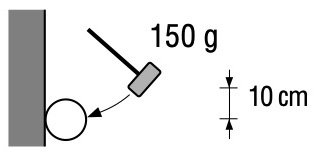
\includegraphics[scale=1]{K1.png}		& \SI{0,15}{\joule}	& 										& 								\\
02 				& 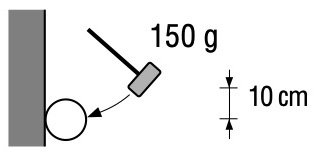
\includegraphics[scale=1]{K1.png}		& \SI{0,20}{\joule}	& 	AG1								& 1							\\
03 				& 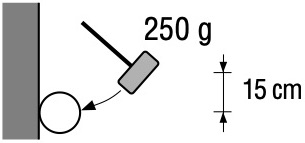
\includegraphics[scale=1]{K3.png}		& \SI{0,35}{\joule}	& 										& 								\\
04 				& 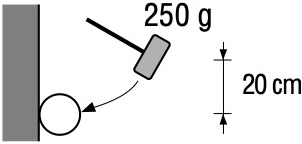
\includegraphics[scale=1]{K4.png}		& \SI{0,50}{\joule}	& 										& 3							\\
05 				& 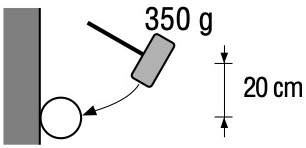
\includegraphics[scale=1]{K5.png}		& \SI{0,70}{\joule}	& 										& 								\\
06 				& 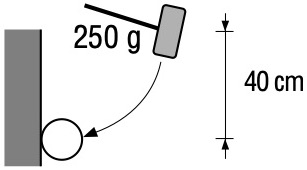
\includegraphics[scale=1]{K6.png}		& \SI{1}{\joule}		& 										& 								\\
07 				& 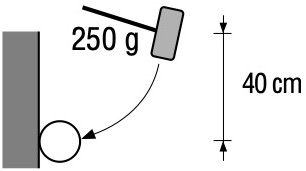
\includegraphics[scale=1]{K7.png}		& \SI{2}{\joule}		& 	AG2								& 5							\\
08 				& 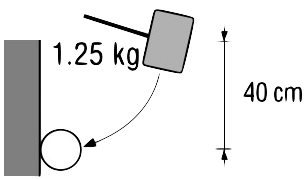
\includegraphics[scale=1]{K8.png}		& \SI{5}{\joule}		& 	AG3								& 								\\
08 				& 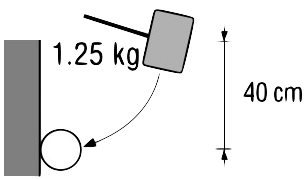
\includegraphics[scale=1]{K8.png}		& \SI{5}{\joule}		& 	AG3								& 								\\
09 				& 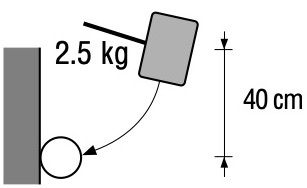
\includegraphics[scale=1]{K9.png}		& \SI{10}{\joule}		& 	AG3								& 								\\
10 				& 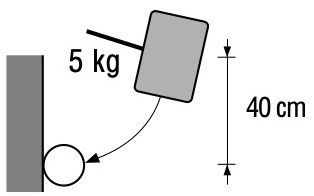
\includegraphics[scale=1]{K10.png}	& \SI{20}{\joule}		& 	AG4								& 								\\
\bottomrule
\end{tabularx}
\begin{tablenotes}
    \item[1] Corresponsdances avec le code AG de la classification des influences externes issu de la norme NF C 15-100.
\end{tablenotes}
\end{threeparttable} %note dans tableau
\end{table}
\end{minipage}
\hfill
\begin{minipage}[t]{0.39\linewidth}
\begin{table}[H]
\caption{Lettre additionnelle sur les informations supplémentaires}
\begin{tabularx}{\linewidth}{P{1.5cm} X}
\toprule
\thead{Lettre}		& \thead{Signification} \\
\midrule
f							& Résistant aux huiles \\
\addlinespace
H							& Appareil à haute tension \\
\addlinespace
M							& Appareil en déplacement durant le test à l'eau \\
\addlinespace
S							& Appareil immobile durant le test à l'eau \\
\addlinespace
W							& Conditions environnementales spécifiées \\
\bottomrule
\end{tabularx}
\end{table}
\end{minipage}

\newpage
\begin{landscape}
\newpage

%--------------------------------------
%ELECTROTECHNIQUE - SCHEMA DE LIAISON A LA TERRE
%--------------------------------------

%utiliser les environnement \begin{comment} \end{comment} pour mettre en commentaire le préambule une fois la programmation appelée dans le document maître (!ne pas oublier de mettre en commentaire \end{document}!)

\begin{comment}

\documentclass[a4paper, 11pt, twoside, fleqn]{memoir}

\usepackage{AOCDTF}

%--------------------------------------
%CANEVAS
%--------------------------------------

\newcommand\BoxColor{\ifcase\thechapshift blue!30\or brown!30\or pink!30\or cyan!30\or green!30\or teal!30\or purple!30\or red!30\or olive!30\or orange!30\or lime!30\or gray!\or magenta!30\else yellow!30\fi} %définition de la couleur des marqueurs de chapitre

\newcounter{chapshift} %compteur de chapitre du marqueur de chapitre
\addtocounter{chapshift}{-1}
	
\newif\ifFrame %instruction conditionnelle pour les couleurs des pages
\Frametrue

\pagestyle{plain}

% the main command; the mandatory argument sets the color of the vertical box
\newcommand\ChapFrame{%
\AddEverypageHook{%
\ifFrame
\ifthenelse{\isodd{\value{page}}}
  {\backgroundsetup{contents={%
  \begin{tikzpicture}[overlay,remember picture]
  \node[
  	rounded corners=3pt,
    fill=\BoxColor,
    inner sep=0pt,
    rectangle,
    text width=1.5cm,
    text height=5.5cm,
    align=center,
    anchor=north west
  ] 
  at ($ (current page.north west) + (-0cm,-2*\thechapshift cm) $) %nombre négatif = espacement des marqueurs entre les différents chapitres (à régler en fin de rédaction) (4.5cm vaut un espacement équivalement à la hauteur du marqueur, une page peut en contenir 6 avec cet espacement-la mais il est le plus équilibré)
    {\rotatebox{90}{\hspace*{.5cm}%
      \parbox[c][1.2cm][t]{5cm}{%
        \raggedright\textcolor{black}{\sffamily\textbf{\leftmark}}}}};
  \end{tikzpicture}}}
  }
  {\backgroundsetup{contents={%
  \begin{tikzpicture}[overlay,remember picture]
  \node[
  	rounded corners=3pt,
    fill=\BoxColor,
    inner sep=0pt,
    rectangle,
    text width=1.5cm,
    text height=5.5cm,
    align=center,
    anchor=north east
  ] 
  at ($ (current page.north east) + (-0cm,-2*\thechapshift cm) $) %nombre négatif = espacement des marqueurs entre les différents chapitres (à régler en fin de rédaction) (4.5cm vaut un espacement équivalement à la hauteur du marqueur, une page peut en contenir 6 avec cet espacement-la mais il est le plus équilibré)
    {\rotatebox{90}{\hspace*{.5cm}%
      \parbox[c][1.2cm][t]{5cm}{%
        \raggedright\textcolor{black}{\sffamily\textbf{\leftmark}}}}};
  \end{tikzpicture}}}%
  }
  \BgMaterial%
  \fi%
}%
  \stepcounter{chapshift}
}

\renewcommand\chaptermark[1]{\markboth{\thechapter.~#1}{}} %redéfinition du marqueur de chapitre pour ne contenir que le titre du chapitre %à personnaliser selon le nombre de chapitre dans le cours

%--------------------------------------
%corps du document
%--------------------------------------

\begin{document} %corps du document
	\openleft %début de chapitre à gauche

\end{comment}

\begin{xltabular}{\linewidth}{p{0.3cm} m{2cm} X p{0.3cm} m{2cm} X p{0.3cm} m{2.2cm} X}
\caption{Descriptif des indices de protection} 
\\
\toprule
\multicolumn{3}{c}{\thead{Protection contre les corps solides}}	& \multicolumn{3}{c}{\thead{Lettre additionnelle\\Contact direct avec les parties dangereuses}}	& \multicolumn{3}{c}{\thead{Protection contre les liquides}} \\
\midrule
\endfirsthead %en-tête de la première page du tableau  

\toprule
\multicolumn{3}{c}{\thead{Protection contre les corps solides}}	& \multicolumn{3}{c}{\thead{Lettre additionnelle\\Contact direct avec les parties dangereuses}}	& \multicolumn{3}{c}{\thead{Protection contre les liquides}} \\
\midrule
\endhead %en-tête de la première page du tableau  

\addlinespace
\midrule %filet de milieu de tableau
\multicolumn{9}{r}{\small\textit{Page suivante}}
\endfoot %pied de page de toutes les pages du tableau

\bottomrule
\endlastfoot %pied de page de la dernièredu tableau

0 		& 									& Aucune protection	&	&	&	& 0 	&	&	Aucune protection \\
1 		& 	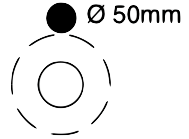
\includegraphics[scale=1.1]{1X.png} & Protégé contre les corps solides $\diameter \geq \SI{50}{\milli\meter}$  	&	A & 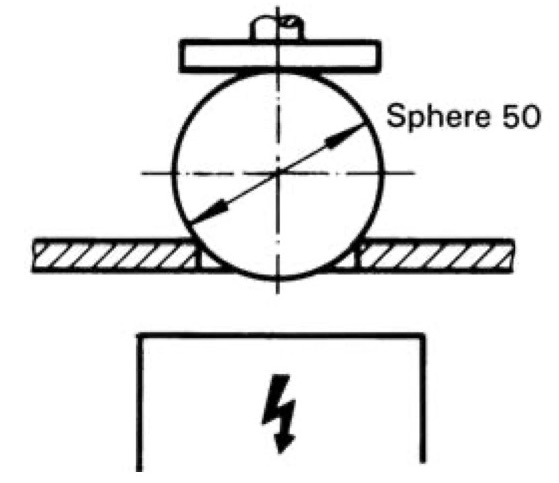
\includegraphics[width=2cm]{A.png}	&	Le dos de la main reste éloigné des parties dangereuses.	& 1 & 	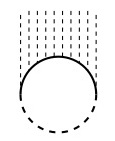
\includegraphics[scale=1.1]{X1.png}	&	Protégé contre les chutes verticales de gouttes d'eau (condensation) \\
2 		& 	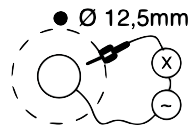
\includegraphics[scale=1.1]{2X.png} & Protégé contre les corps solides $\diameter \geq \SI{12,5}{\milli\meter}$  	& B	& 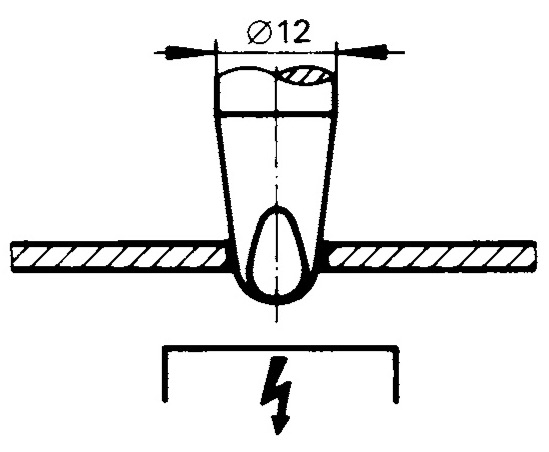
\includegraphics[width=2cm]{B.png}	&	L'introduction d'un doigt ne permet pas de toucher les parties dangereuses. & 2 & 	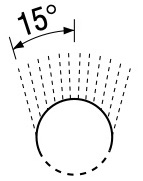
\includegraphics[scale=1.1]{X2.png}	&	Protégé contre les chutes de gouttes d'eau jusqu'à 15° de la verticale \\
3 		& 	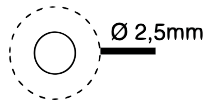
\includegraphics[scale=1.1]{3X.png} & Protégé contre les corps solides $\diameter \geq \SI{2,5}{\milli\meter}$  	& C	& 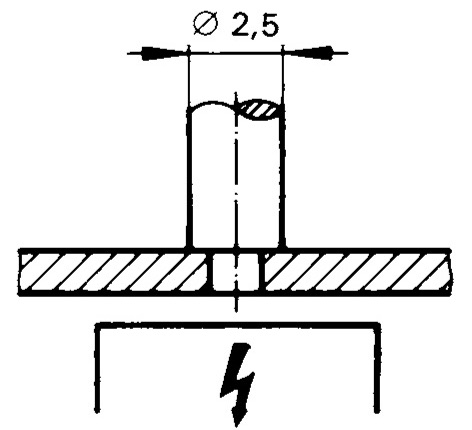
\includegraphics[width=2cm]{C.png}	&	L'introduction d'un outil ne permet pas de toucher les parties dangereuses. & 3 & 	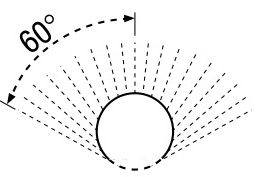
\includegraphics[scale=1.1]{X3.png}	&	Protégé contre l'eau de pluie jusqu'à 60° de la verticale \\
4 		& 	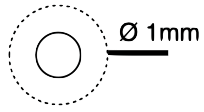
\includegraphics[scale=1.1]{4X.png} & Protégé contre les corps solides $\diameter \geq \SI{1}{\milli\meter}$  	& D	& 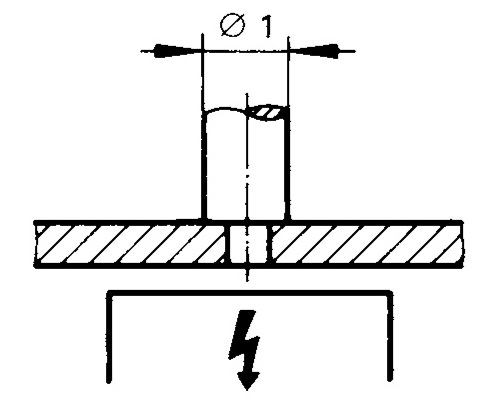
\includegraphics[width=2cm]{D.png}	&	L'introduction d'un outil fin ne permet pas de toucher les parties dangereuses. & 4 & 	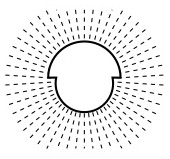
\includegraphics[scale=1.1]{X4.png}	&	Protégé contre les projections d'eau dans toutes les directions \\
5 		& 	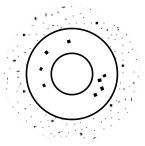
\includegraphics[scale=1.1]{5X.png} & Protégé contre la poussière (pas de dépot nuisible)  	& 	& & & 5 & 	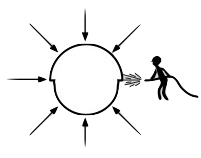
\includegraphics[scale=1.1]{X5.png}	&	Protégé contre les jets d'eau dans toutes les directions à la lance \\
6 		& 	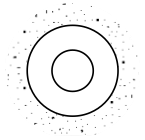
\includegraphics[scale=1.1]{6X.png} & Totalement protégé contre la poussière 	& 	& & & 6 & 	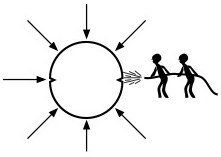
\includegraphics[scale=1.1]{X6.png}	&	Protégé contre les projections d'eau assimilables aux paquets de mer \\
 		&  & 	& 	& & & 7 & 	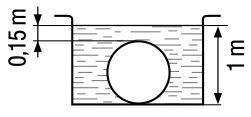
\includegraphics[scale=1.1]{X7.png}	&	Protégé contre les effets d'une immersion temporaire dans l'eau \\
		&  & 	& 	& & & 8 & 	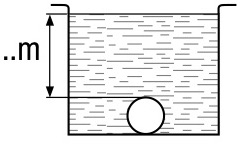
\includegraphics[scale=1.1]{X8.png}	&	Protégé contre les effets d'une immersion prolongée dans l'eau dans des conditions spécifiées \\
		&  & 	& 	& & & 9\tnote{1} & 	&	Protégé contre les jets d'eau haute pression et haute température mais pas nécessairement submersible \\
\end{xltabular}	


%\end{document}



\newpage
\end{landscape}
\newpage

\subsubsection{Classification des locaux selon l'IP}

Selon les locaux à équiper, leurs emplacements et les conditions particulières d'installation, la norme NF C 15-100 indique une protection minimale spécifiée par les indices IP et IK.

%--------------------------------------
%ELECTROTECHNIQUE - SCHEMA DE LIAISON A LA TERRE
%--------------------------------------

%utiliser les environnement \begin{comment} \end{comment} pour mettre en commentaire le préambule une fois la programmation appelée dans le document maître (!ne pas oublier de mettre en commentaire \end{document}!)

\begin{comment}

\documentclass[a4paper, 11pt, twoside, fleqn]{memoir}

\usepackage{AOCDTF}

%--------------------------------------
%CANEVAS
%--------------------------------------

\newcommand\BoxColor{\ifcase\thechapshift blue!30\or brown!30\or pink!30\or cyan!30\or green!30\or teal!30\or purple!30\or red!30\or olive!30\or orange!30\or lime!30\or gray!\or magenta!30\else yellow!30\fi} %définition de la couleur des marqueurs de chapitre

\newcounter{chapshift} %compteur de chapitre du marqueur de chapitre
\addtocounter{chapshift}{-1}
	
\newif\ifFrame %instruction conditionnelle pour les couleurs des pages
\Frametrue

\pagestyle{plain}

% the main command; the mandatory argument sets the color of the vertical box
\newcommand\ChapFrame{%
\AddEverypageHook{%
\ifFrame
\ifthenelse{\isodd{\value{page}}}
  {\backgroundsetup{contents={%
  \begin{tikzpicture}[overlay,remember picture]
  \node[
  	rounded corners=3pt,
    fill=\BoxColor,
    inner sep=0pt,
    rectangle,
    text width=1.5cm,
    text height=5.5cm,
    align=center,
    anchor=north west
  ] 
  at ($ (current page.north west) + (-0cm,-2*\thechapshift cm) $) %nombre négatif = espacement des marqueurs entre les différents chapitres (à régler en fin de rédaction) (4.5cm vaut un espacement équivalement à la hauteur du marqueur, une page peut en contenir 6 avec cet espacement-la mais il est le plus équilibré)
    {\rotatebox{90}{\hspace*{.5cm}%
      \parbox[c][1.2cm][t]{5cm}{%
        \raggedright\textcolor{black}{\sffamily\textbf{\leftmark}}}}};
  \end{tikzpicture}}}
  }
  {\backgroundsetup{contents={%
  \begin{tikzpicture}[overlay,remember picture]
  \node[
  	rounded corners=3pt,
    fill=\BoxColor,
    inner sep=0pt,
    rectangle,
    text width=1.5cm,
    text height=5.5cm,
    align=center,
    anchor=north east
  ] 
  at ($ (current page.north east) + (-0cm,-2*\thechapshift cm) $) %nombre négatif = espacement des marqueurs entre les différents chapitres (à régler en fin de rédaction) (4.5cm vaut un espacement équivalement à la hauteur du marqueur, une page peut en contenir 6 avec cet espacement-la mais il est le plus équilibré)
    {\rotatebox{90}{\hspace*{.5cm}%
      \parbox[c][1.2cm][t]{5cm}{%
        \raggedright\textcolor{black}{\sffamily\textbf{\leftmark}}}}};
  \end{tikzpicture}}}%
  }
  \BgMaterial%
  \fi%
}%
  \stepcounter{chapshift}
}

\renewcommand\chaptermark[1]{\markboth{\thechapter.~#1}{}} %redéfinition du marqueur de chapitre pour ne contenir que le titre du chapitre %à personnaliser selon le nombre de chapitre dans le cours

%--------------------------------------
%corps du document
%--------------------------------------

\begin{document} %corps du document
	\openleft %début de chapitre à gauche

\end{comment}

\captionof{table}{Classification des locaux}
\vspace{-1em}
\begin{minipage}[t]{0.49\linewidth}
\begin{tabularx}{\textwidth}[t]{c X c c}
\toprule
\multicolumn{2}{c}{\thead{Type de\\local}}																				& \thead{IP}	& \thead{IK}  \\
\midrule
\multicolumn{4}{p{0.95\textwidth}}{\textit{Locaux (ou emplacements) domestiques et analogues}} \\
\middashrule \\
\multicolumn{2}{p{4.8cm}}{Auvents}																							& 24				& 07 \\
\multicolumn{2}{p{4.8cm}}{Bains (salle de)}																				& \multicolumn{2}{p{2.2cm}}{(voir salles d'eau)} \\
\multicolumn{2}{p{4.8cm}}{Bicyclettes, cyclomoteurs, voitures pour enfants (locaux pour)}			& 20				& 07 \\
\multicolumn{2}{p{4.8cm}}{Branchement eau, égout, chauffage}												& 23				& 02 \\
\multicolumn{2}{p{4.8cm}}{Buanderies}																					& 23				& 02 \\
\multicolumn{2}{p{4.8cm}}{Caves, celliers, garage, local avec chaudière}									& 20				& 02--07 \\
\multicolumn{2}{p{4.8cm}}{Chambres	}																					& 20				& 02 \\
\multicolumn{2}{p{4.8cm}}{Collecte des ordures (locaux pour)}												& 25				& 07 \\
\multicolumn{2}{p{4.8cm}}{Couloirs de cave}																			& 20				& 07 \\
\multicolumn{2}{p{4.8cm}}{Cours}																							& 24--25			& 02--07 \\
\multicolumn{2}{p{4.8cm}}{Cuisines}																						& 20				& 02 \\
\multicolumn{2}{p{4.8cm}}{Douches}																						& \multicolumn{2}{p{2.2cm}}{(voir salles d'eau)} \\
\multicolumn{2}{p{4.8cm}}{Escaliers intérieurs, coursives intérieures}										& 20				& 02--07 \\
\multicolumn{2}{p{4.8cm}}{Escaliers extérieures, coursives extérieures non couvertes}				& 24				& 07 \\
\multicolumn{2}{p{4.8cm}}{Coursives extérieures couvertes}														& 21				& 02 \\
\multicolumn{2}{p{4.8cm}}{Greniers (combles)}																			& 20				& 02 \\
\multicolumn{2}{p{4.8cm}}{Abris de jardins	}																			& 24--25			& 02--07 \\
\multicolumn{2}{p{4.8cm}}{Lieux d'aisances}																			& 20				& 02 \\
\multicolumn{2}{p{4.8cm}}{Locaux à poubelles}																		& 25				& 02--07 \\
\multicolumn{2}{p{4.8cm}}{Lingeries, salles de repassage}														& 21				& 02 \\
\multicolumn{2}{p{4.8cm}}{Rampes d'accès au garage}																& 25				& 07 \\
\multicolumn{2}{p{4.8cm}}{Salles d'eau, locaux contenant une baignoire ou une douche :	}		& 					& \\
& volume 0																& 27				& 02 \\
& volume 1																& 24				& 02 \\
& volume 2																& 23				& 02 \\
& volume 3																& 21				& 02 \\
\multicolumn{2}{p{4.8cm}}{Salles de séjour}																				& 20				& 02 \\
\multicolumn{2}{p{4.8cm}}{Séchoirs}																						& 21				& 02 \\
\end{tabularx}
\end{minipage}
\hfill
\begin{minipage}[t]{0.49\linewidth}
\begin{tabularx}{\textwidth}[t]{c X c c}
\toprule
\multicolumn{2}{c}{\thead{Type de\\local}}																				& \thead{IP}	& \thead{IK}  \\
\midrule
\multicolumn{4}{p{0.95\textwidth}}{\textit{Locaux (ou emplacements) domestiques et analogues}} \\
\middashrule \\
\multicolumn{2}{p{4.8cm}}{Sous-sols}																						& 21				& 02/07 \\
\multicolumn{2}{p{4.8cm}}{Terrasses couvertes}																		& 21				& 02 \\
\multicolumn{2}{p{4.8cm}}{Toilettes (cabinets de)}																	& 21				& 02 \\
\multicolumn{2}{p{4.8cm}}{Vérandas}																						& 21				& 02 \\
\multicolumn{2}{p{4.8cm}}{Vides sanitaires}																				& 23				& 02--07 \\
\addlinespace
\midrule
\multicolumn{4}{p{0.95\textwidth}}{\textit{Locaux techniques}} \\
\middashrule \\
\multicolumn{2}{p{4.8cm}}{Accumulateurs (salles d')}																& 23				& 02--07 \\
\multicolumn{2}{p{4.8cm}}{Ascenseurs (locaux des machines et locaux des poulies)}					& 20				& 07--08 \\	
\multicolumn{2}{p{4.8cm}}{Service électrique}																			& 20				& 07 \\
\multicolumn{2}{p{4.8cm}}{Salles des commandes}																	& 20				& 02 \\
\multicolumn{2}{p{4.8cm}}{Ateliers}																							& 21--23			& 07--08 \\
\multicolumn{2}{p{4.8cm}}{Laboratoires}																					& 21--23			& 02--07 \\
\multicolumn{2}{p{4.8cm}}{Laveurs de conditionnement d'air	}													& 24				& 07 \\
\multicolumn{2}{p{4.8cm}}{Garages (servant exclusivement au stationnement des véhicules) d'une surface n'excédant pas \SI{100}{\square\meter}}	& 21				& 07 \\
\multicolumn{2}{p{4.8cm}}{Laveurs de conditionnement d'air}													& 24				& 07 \\
\multicolumn{2}{p{4.8cm}}{Machines (salles de)}																		& 31				& 07--08 \\
\multicolumn{2}{p{4.8cm}}{Surpresseurs d'eau}																		& 23				& 07--08 \\
\multicolumn{2}{p{4.8cm}}{Chaufferies et locaux annexes :}														& 					& \\
&	 à charbon																																& 51--61			& 07--08 \\
&	 autres combustibles																												& 21				& 07--08 \\
&	 électriques																															& 21				& 07--08 \\
\addlinespace
\midrule
\multicolumn{4}{p{0.95\textwidth}}{\textit{Garages et parcs de stationnement couverts d'une surface supérieure à \SI{100}{\square\meter}}} \\
\middashrule \\
\multicolumn{2}{p{4.8cm}}{Aires de stationnement}																	& 21				& 07--20 \\
\multicolumn{2}{p{4.8cm}}{Zones de lavage (à l'intérieur du local)}											& 25				& 07 \\
\multicolumn{2}{p{4.8cm}}{Zones de sécurité :}																		& 					&  \\
	&	à l'intérieur																														& 21				& 07 \\
	&	à l'extérieur																														& 24				& 07 \\
\multicolumn{2}{p{4.8cm}}{Zones de graissage}																			& 23				& 08 \\

\end{tabularx}
\end{minipage}
\begin{minipage}{0.49\textwidth}
\begin{tabularx}{\textwidth}{R}
\midrule
\small\textit{Colonne suivante} \\
\end{tabularx}
\end{minipage}
\hfill
\begin{minipage}{0.49\textwidth}
\begin{tabularx}{\textwidth}{R}
\midrule
\small\textit{Page suivante} \\
\end{tabularx}
\end{minipage}
\begin{minipage}[t]{0.49\linewidth}
\begin{tabularx}{\textwidth}[t]{c X c c}
\multicolumn{4}{l}{\small\textit{Page précédente}} \\
\midrule
\multicolumn{2}{c}{\thead{Type de\\local}}																				& \thead{IP}	& \thead{IK}  \\
\midrule
\multicolumn{4}{p{0.95\textwidth}}{\textit{Garages et parcs de stationnement couverts d'une surface supérieure à \SI{100}{\square\meter}}} \\
\middashrule \\
\multicolumn{2}{p{4.8cm}}{Locaux de recharge de batteries}															& 23				& 07 \\
\multicolumn{2}{p{4.8cm}}{Ateliers}																								& 21				& 08 \\
\addlinespace
\midrule
\multicolumn{4}{p{0.95\textwidth}}{\textit{Locaux sanitaires à usage collectif}} \\
\middashrule \\
\multicolumn{2}{p{4.8cm}}{Salles de lavabos individuels}																& 21				& 07 \\
\multicolumn{2}{p{4.8cm}}{Salles de WC à cuvettes (à l'anglaise)}													& 21				& 07 \\
\multicolumn{2}{p{4.8cm}}{Salles d'urinoirs}																					& 21				& 07 \\
\multicolumn{2}{p{4.8cm}}{Salles de lavabos collectifs}																	& 23				& 07 \\
\multicolumn{2}{p{4.8cm}}{Salles de WC à la turques, de douches à cabines individuelles, de douches collectives}								& 23				& 07 \\
\multicolumn{2}{p{4.8cm}}{Buanderies collectives}																		& 24				& 07 \\
\addlinespace
\midrule
\multicolumn{4}{p{0.95\textwidth}}{\textit{Bâtiments à usage collectif (autre que ERP)}} \\
\middashrule \\
\multicolumn{2}{p{4.8cm}}{Bureaux}																							& 20				& 02 \\
\multicolumn{2}{p{4.8cm}}{Bibliothèques}																					& 20				& 02 \\
\multicolumn{2}{p{4.8cm}}{Salles d'archives}																				& 20				& 02 \\
\multicolumn{2}{p{4.8cm}}{Salles d'informatiques}																		& 20				& 02 \\
\multicolumn{2}{p{4.8cm}}{Salles de dessin}																					& 20				& 02 \\
\multicolumn{2}{p{4.8cm}}{Locaux regroupant les machines de reproduction de plans et de documents}			& 20				& 02 \\
\multicolumn{2}{p{4.8cm}}{Salles de tri}																						& 20				& 07 \\
\multicolumn{2}{p{4.8cm}}{Salles de restaurant et de cantine, grandes cuisines}							& 21				& 07 \\
\multicolumn{2}{p{4.8cm}}{Salles de sports}																					& 21				& 07--08 \\
\multicolumn{2}{p{4.8cm}}{Locaux de casernement}																		& 21				& 07 \\
\multicolumn{2}{p{4.8cm}}{Salles de réunion}																				& 20				& 02 \\
\multicolumn{2}{p{4.8cm}}{Salles d'attentes, salons, hall}																& 20				& 02 \\
\multicolumn{2}{p{4.8cm}}{Salles de consultation à usage médical, ne comportant pas d'équipements spécifiques}		& 20				& 02 \\
\multicolumn{2}{p{4.8cm}}{Salles de démonstration et d'exposition}												& 20				& 02 \\
\addlinespace
\midrule
\multicolumn{4}{p{0.95\textwidth}}{\textit{Locaux (ou emplacements) dans les exploitations agricoles}} \\
\middashrule \\
\multicolumn{2}{p{4.8cm}}{Alcools (entrepôts de)}																		& 23				& 07 \\
\end{tabularx}
\end{minipage}
\hfill
\begin{minipage}[t]{0.49\linewidth}
\begin{tabularx}{\textwidth}[t]{c X c c}
\multicolumn{4}{l}{\small\textit{Colonne précédente}} \\
\midrule
\multicolumn{2}{c}{\thead{Type de\\local}}																				& \thead{IP}	& \thead{IK}  \\
\midrule
\multicolumn{4}{p{0.95\textwidth}}{\textit{Locaux (ou emplacements) dans les exploitations agricoles}} \\
\middashrule \\
\multicolumn{2}{p{4.8cm}}{Bergeries fermées}																				& 35				& 07 \\
\multicolumn{2}{p{4.8cm}}{Buanderies}																					& 24				& 07 \\
\multicolumn{2}{p{4.8cm}}{Battages de céréales}																		& 50				& 07 \\
\multicolumn{2}{p{4.8cm}}{Bûchers}																							& 30				& 10 \\
\multicolumn{2}{p{4.8cm}}{Caves de distillation}																		& 23				& 07 \\
\multicolumn{2}{p{4.8cm}}{Chais (vin)	}																					& 23				& 07 \\
\multicolumn{2}{p{4.8cm}}{Cours}																							& 35				& 07 \\
\multicolumn{2}{p{4.8cm}}{\'Elevages de volailles}																	& 35				& 07 \\
\multicolumn{2}{p{4.8cm}}{\'Ecuries}																						& 35				& 07 \\
\multicolumn{2}{p{4.8cm}}{Engrais (dépôts d')}																			& 50				& 07 \\
\multicolumn{2}{p{4.8cm}}{\'Etables}																						& 35				& 07 \\
\multicolumn{2}{p{4.8cm}}{Fumières}																						& 24				& 07 \\
\multicolumn{2}{p{4.8cm}}{Fenils}																							& 50				& 07 \\
\multicolumn{2}{p{4.8cm}}{Fourrage (entrepôts de)}																	& 50				& 07 \\
\multicolumn{2}{p{4.8cm}}{Greniers, granges}																			& 50				& 07 \\
\multicolumn{2}{p{4.8cm}}{Paille (entrepôts de)}																		& 50				& 07 \\
\multicolumn{2}{p{4.8cm}}{Serres}																							& 23				& 07 \\
\multicolumn{2}{p{4.8cm}}{Silos à céréales}																				& 50				& 07 \\
\multicolumn{2}{p{4.8cm}}{Traies (salle de)}																				& 35				& 07 \\
\multicolumn{2}{p{4.8cm}}{Porcheries}																						& 35				& 07 \\
\multicolumn{2}{p{4.8cm}}{Poulaillers}																						& 35				& 07 \\
\addlinespace
\midrule
\multicolumn{4}{p{0.95\textwidth}}{\textit{Installations diverses}} \\
\middashrule \\
\multicolumn{2}{p{4.8cm}}{Terrains de camping et caravaning}													& 34				& 07 \\
\multicolumn{2}{p{4.8cm}}{Quais de ports de plaisance}															& 34				& 08 \\
\multicolumn{2}{p{4.8cm}}{Chantiers}																						& 44				& 08 \\
\multicolumn{2}{p{4.8cm}}{Quais de chargement}																		& 35				& 08 \\
\multicolumn{2}{p{4.8cm}}{Rues, cours, jardins et autres emplacements extérieurs}					& 34--35			& 07 \\
\multicolumn{2}{p{4.8cm}}{\'Etablissement forains}																	& 33				& 08 \\
\multicolumn{2}{p{4.8cm}}{Piscines :}																						& 					&	  \\
& volume 0																																& 28				& 02 \\
& volume 1																																& 25				& 02 \\
& volume 2																																& 22--24			& 02 \\
\multicolumn{2}{p{4.8cm}}{Saunas}																							& 34				& 02 \\
\multicolumn{2}{p{4.8cm}}{Bassins de fontaines}																		& 37				& 02 \\
\multicolumn{2}{p{4.8cm}}{Traitements des eaux (local de)}														& 24--25			& 07--08 \\
\addlinespace
\midrule
\multicolumn{4}{p{0.95\textwidth}}{\textit{Installations thermodynamiques, chambres climatisées et chambres froides}} \\
\middashrule \\
\end{tabularx}
\end{minipage}
\begin{minipage}[b]{0.49\textwidth}
\begin{xltabular}{\textwidth}{R}
\midrule
\small\textit{Colonne suivante} \\
\end{xltabular}
\end{minipage}
\hfill
\begin{minipage}[b]{0.49\textwidth}
\begin{xltabular}{\textwidth}{R}
\midrule
\small\textit{Page suivante} \\
\end{xltabular}
\end{minipage}
\begin{minipage}[t]{0.49\linewidth}
\begin{tabularx}{\textwidth}[t]{c X c c}
\multicolumn{4}{l}{\small\textit{Page précédente}} \\
\midrule
\multicolumn{2}{c}{\thead{Type de\\local}}																				& \thead{IP}	& \thead{IK}  \\
\midrule
\multicolumn{4}{p{0.95\textwidth}}{\textit{Installations thermodynamiques, chambres climatisées et chambres froides}} \\
\middashrule \\
\multicolumn{2}{p{4.8cm}}{Température < \SI{-10}{\celsius}}												&	23				&	07 \\	
\multicolumn{2}{p{4.8cm}}{Hauteur au dessus du sol :}															& 					&  \\
& \SIrange[range-phrase=\ à\ ]{0}{1,10}{\meter}																		& 24				& 07 \\
& \SIrange[range-phrase=\ à\ ]{1,10}{2}{\meter}																		& 21				& 07 \\
& au-dessus de \SI{2}{\meter}																									& 21				& 07 \\
& sous l'évaporateur ou tube																									& 21				& 07 \\
& écoulement d'eau																													& 21				& 07 \\
\multicolumn{2}{p{4.8cm}}{Plafond et jusqu'à \SI{10}{\centi\meter} en-dessous}	 				&	23				&	07 \\	
\multicolumn{2}{p{4.8cm}}{Compresseur :}																			& 					&  \\
& local																																		& 21				& 08 \\
& monobloc placé à l'extérieur ou en terrasse																				& 34				& 08 \\
\midrule
\multicolumn{4}{p{0.95\textwidth}}{\textit{\'Etablissements industriels}} \\
\middashrule \\
\multicolumn{2}{p{4.8cm}}{Abattoirs}																	 				&	55				&	08 \\	
\multicolumn{2}{p{4.8cm}}{Accumulateurs (fabrication d')}										 				&	33				&	07 \\	
\multicolumn{2}{p{4.8cm}}{Acide (fabrication et dépôts)}										 				&	33				&	07 \\	
\multicolumn{2}{p{4.8cm}}{Alcool (fabrication et dépôts)}										 				&	33				&	07 \\	
\multicolumn{2}{p{4.8cm}}{Aluminium (fabrication et dépôts)}										 		&	51--53		&	08 \\	
\multicolumn{2}{p{4.8cm}}{Animaux (élevage et engraissement)}										 	&	45				&	07 \\	
\multicolumn{2}{p{4.8cm}}{Asphaltes, bitume (dépôts d')}										 				&	53				&	07 \\	
\multicolumn{2}{p{4.8cm}}{Battage et cardage des laines}											 				&	50				&	08 \\	
\multicolumn{2}{p{4.8cm}}{Blanchisseries}																 				&	23--24		&	07 \\	
\multicolumn{2}{p{4.8cm}}{Bois (travail du)}																 			&	50				&	08 \\
\multicolumn{2}{p{4.8cm}}{Boucheries}																		 			&	24--25		&	07 \\	
\multicolumn{2}{p{4.8cm}}{Boucheries}																		 			&	24--25		&	07 \\	
\multicolumn{2}{p{4.8cm}}{Brasseries}																		 			&	24				&	07 \\	
\multicolumn{2}{p{4.8cm}}{Briqueteries}																		 		&	53--54		&	08 \\	
\multicolumn{2}{p{4.8cm}}{Caoutchouc (fabrication et transformation)}								 	&	54				&	07 \\	
\multicolumn{2}{p{4.8cm}}{Carbure (fabrication et dépôts)}								 					&	51				&	07 \\	
\multicolumn{2}{p{4.8cm}}{Cartoucherie}								 												&	53				&	08 \\	
\multicolumn{2}{p{4.8cm}}{Cartons (fabrication de}																&	33				&	07 \\	
\multicolumn{2}{p{4.8cm}}{Carrières}									 												&	55				&	08 \\
\multicolumn{2}{p{4.8cm}}{Celluloïd (fabrication d'objets}														&	30				&	08 \\	
\multicolumn{2}{p{4.8cm}}{Cellulose (fabrication)}									 								&	34				&	08 \\	
\end{tabularx}
\end{minipage}
\hfill
\begin{minipage}[t]{0.49\linewidth}
\begin{tabularx}{\textwidth}[t]{c X c c}
\multicolumn{4}{l}{\small\textit{Colonne précédente}} \\
\midrule
\multicolumn{2}{c}{\thead{Type de\\local}}																				& \thead{IP}	& \thead{IK}  \\
\midrule
\multicolumn{4}{p{0.95\textwidth}}{\textit{\'Etablissements industriels}} \\
\middashrule \\
\multicolumn{2}{p{4.8cm}}{Charbon (entrepôts de)}									 							&	54				&	08 \\	
\multicolumn{2}{p{4.8cm}}{Charcuteries}									 											&	24				&	07 \\	
\multicolumn{2}{p{4.8cm}}{Chaudronneries}									 										&	30				&	08 \\	
\multicolumn{2}{p{4.8cm}}{Chaux (fours à)}									 										&	50				&	08 \\	
\multicolumn{2}{p{4.8cm}}{Chiffons (entrepôts de)}									 							&	30				&	07 \\	
\multicolumn{2}{p{4.8cm}}{Chlore (fabrication et dépôts)}									 					&	33				&	07 \\	
\multicolumn{2}{p{4.8cm}}{Chromage}									 												&	33				&	07 \\	
\multicolumn{2}{p{4.8cm}}{Cimenterie}									 												&	50				&	08 \\	
\multicolumn{2}{p{4.8cm}}{Cokerie}									 													&	53				&	08 \\	
\multicolumn{2}{p{4.8cm}}{Colle (fabrication de)}									 								&	33				&	07 \\
\multicolumn{2}{p{4.8cm}}{Chaines d'embouteillage}									 							&	35				&	08 \\	
\multicolumn{2}{p{4.8cm}}{Combustibles liquides (dépôts de)}												&	31--33		&	08 \\	
\multicolumn{2}{p{4.8cm}}{Corps gras (traitement de)}									 						&	51				&	07 \\	
\multicolumn{2}{p{4.8cm}}{Cuir (fabrication et dépôts de)}									 					&	31				&	08 \\	
\multicolumn{2}{p{4.8cm}}{Cuivre (traitement des minéraux)}									 				&	31				&	08 \\	
\multicolumn{2}{p{4.8cm}}{Décapage}									 												&	54				&	08 \\	
\multicolumn{2}{p{4.8cm}}{Détersifs (fabrication de produits)}									 			&	53				&	07 \\	
\multicolumn{2}{p{4.8cm}}{Distillerie}									 												&	33				&	07 \\	
\multicolumn{2}{p{4.8cm}}{\'Electrolyse}									 											&	03				&	08 \\	
\multicolumn{2}{p{4.8cm}}{Encre (fabrication d')}									 								&	31				&	07 \\	
\multicolumn{2}{p{4.8cm}}{Engrais (fabrication et dépôts de)}				 								&	53				&	07 \\	
\multicolumn{2}{p{4.8cm}}{Explosifs (fabrication et dépôts de)}				 								&	55				&	08 \\	
\multicolumn{2}{p{4.8cm}}{Fer (fabrication et traitement de)}				 									&	51				&	08 \\	
\multicolumn{2}{p{4.8cm}}{Filatures}									 													&	50			&	07 \\	
\multicolumn{2}{p{4.8cm}}{Fourrures (battage)}									 									&	50			&	07 \\	
\multicolumn{2}{p{4.8cm}}{Fromageries}									 											&	25			&	07 \\	
\multicolumn{2}{p{4.8cm}}{Gaz (usines et depôts de)}									 						&	31			&	08 \\	
\multicolumn{2}{p{4.8cm}}{Goudron (traitement de)}									 							&	33			&	07 \\	
\multicolumn{2}{p{4.8cm}}{Graineteries}									 											&	50			&	07 \\	
\multicolumn{2}{p{4.8cm}}{Gravures de métaux}																	&	33			&	07 \\	
\multicolumn{2}{p{4.8cm}}{Huile (extraction de)}																	&	31			&	07 \\	
\multicolumn{2}{p{4.8cm}}{Hydrocarbures (fabrication de)}														&	33--34	&	08 \\	
\multicolumn{2}{p{4.8cm}}{Imprimeries}																				&	20			&	08 \\	
\multicolumn{2}{p{4.8cm}}{Laiteries}																						&	25			&	07 \\	
\multicolumn{2}{p{4.8cm}}{Laveries, lavoirs publics}																&	25			&	07 \\	
\multicolumn{2}{p{4.8cm}}{Liqueurs (fabrication de)}																&	21			&	07 \\	
\end{tabularx}
\end{minipage}
\begin{minipage}[b]{0.49\textwidth}
\begin{xltabular}{\textwidth}{R}
\midrule
\small\textit{Colonne suivante} \\
\end{xltabular}
\end{minipage}
\hfill
\begin{minipage}[b]{0.49\textwidth}
\begin{xltabular}{\textwidth}{R}
\midrule
\small\textit{Page suivante} \\
\end{xltabular}
\end{minipage}
\begin{minipage}[t]{0.49\linewidth}
\begin{tabularx}{\textwidth}[t]{c X c c}
\multicolumn{4}{l}{\small\textit{Page précédente}} \\
\midrule
\multicolumn{2}{c}{\thead{Type de\\local}}																				& \thead{IP}	& \thead{IK}  \\
\midrule
\multicolumn{4}{p{0.95\textwidth}}{\textit{\'Etablissements industriels}} \\
\middashrule \\
\multicolumn{2}{p{4.8cm}}{Liquides halogénés (emploi de)}													&	21			&	08 \\	
\multicolumn{2}{p{4.8cm}}{Liquides inflammables (dépôts, ateliers ou l'on emploie des)}			&	21			&	08 \\	
\multicolumn{2}{p{4.8cm}}{Magnésium (fabrication, travail et depôts de)}								&	31			&	07 \\	
\multicolumn{2}{p{4.8cm}}{Machines (salle des)}																	&	20			&	08 \\	
\multicolumn{2}{p{4.8cm}}{Matières plastiques (fabrication de)}												&	51			&	08 \\	
\multicolumn{2}{p{4.8cm}}{Menuiseries}																				&	50			&	08 \\	
\multicolumn{2}{p{4.8cm}}{Métaux (traitement de)}									 							&	31--33	&	08 \\	
\multicolumn{2}{p{4.8cm}}{Moteurs thermiques (essai de)}									 					&	30			&	08 \\	
\multicolumn{2}{p{4.8cm}}{Munitions (dépôts de)}									 								&	33			&	08 \\	
\multicolumn{2}{p{4.8cm}}{Nickel (traitement des minérais)}									 				&	33			&	08 \\	
\multicolumn{2}{p{4.8cm}}{Ordures ménagères (traitement d')}								 				&	53--54	&	07 \\	
\multicolumn{2}{p{4.8cm}}{Papiers (fabriques de)}													 				&	33--34	&	07 \\	
\multicolumn{2}{p{4.8cm}}{Papiers (dépôts de)}													 					&	31			&	07 \\	
\multicolumn{2}{p{4.8cm}}{Parfum (fabrication et dépôts de)}													&	31			&	07 \\	
\multicolumn{2}{p{4.8cm}}{Pâte à papiers (préparation de)}													&	34			&	07 \\	
\multicolumn{2}{p{4.8cm}}{Peinture (fabrication et dépôts de)}												&	33			&	08 \\	
\multicolumn{2}{p{4.8cm}}{Plâtre (broyage et dépôts de)}														&	50			&	07 \\	
\multicolumn{2}{p{4.8cm}}{Poudreries}																					&	55			&	07 \\	
\multicolumn{2}{p{4.8cm}}{Produits chimiques (fabrication de)}												&	30--50	&	08 \\	
\multicolumn{2}{p{4.8cm}}{Raffinerie de pétrole}																	&	34			&	07 \\	
\multicolumn{2}{p{4.8cm}}{Salaisons}																					&	33			&	07 \\	
\multicolumn{2}{p{4.8cm}}{Savons (fabrication de)}																&	31			&	07 \\	
\multicolumn{2}{p{4.8cm}}{Scieries}																						&	50			&	08 \\	
\multicolumn{2}{p{4.8cm}}{Serrureries}																					&	30			&	08 \\	
\multicolumn{2}{p{4.8cm}}{Silos à céréales ou à sucre}															&	50			&	07 \\	
\multicolumn{2}{p{4.8cm}}{Soies et crins (préparation de)}														&	50			&	08 \\	
\multicolumn{2}{p{4.8cm}}{Soude (fabrication et dépôts de)}													&	33			&	07 \\	
\multicolumn{2}{p{4.8cm}}{Soude (traitement de)}																		&	51			&	07 \\	
\multicolumn{2}{p{4.8cm}}{Spiritueux (entrepôts de)}																&	33			&	07 \\	
\multicolumn{2}{p{4.8cm}}{Sucreries}																					&	55			&	07 \\	
\multicolumn{2}{p{4.8cm}}{Tanneries}																					&	35			&	07 \\	
\end{tabularx}
\end{minipage}
\hfill
\begin{minipage}[t]{0.49\linewidth}
\begin{tabularx}{\textwidth}[t]{c X c c}
\multicolumn{4}{l}{\small\textit{Colonne précédente}} \\
\midrule
\multicolumn{2}{c}{\thead{Type de\\local}}																				& \thead{IP}	& \thead{IK}  \\
\midrule
\multicolumn{4}{p{0.95\textwidth}}{\textit{\'Etablissements industriels}} \\
\middashrule \\
\multicolumn{2}{p{4.8cm}}{Teintureries}																				&	35			&	07 \\	
\multicolumn{2}{p{4.8cm}}{Textiles et tissus (fabrication de)}													&	51			&	08 \\	
\multicolumn{2}{p{4.8cm}}{Vernis (fabrication et application de)}											&	33			&	08 \\	
\multicolumn{2}{p{4.8cm}}{Verreries}																					&	33			&	08 \\	
\multicolumn{2}{p{4.8cm}}{Zinc (travail du)}																			&	31			&	08 \\	
\midrule
\multicolumn{4}{p{0.95\textwidth}}{\textit{\'Etablissements recevant du public (ERP)}} \\
\middashrule \\
L 	& \multicolumn{3}{p{0.75\textwidth}}{Salles d'audition, de conférence, de réunion, de spectacles ou à usages multiples :} \\
& salles																																	& 20			& 02--07 \\
& cages de scènes																													& 20			& 08 \\
& magasin de décors																												& 20			& 08 \\
& locaux des perruquiers et des cordonniers																			& 20			& 07 \\
M 	& \multicolumn{3}{p{0.8\textwidth}}{Magasins de vente, centres commerciaux :} \\
& locaux de ventes																												& 20			& 08 \\
& stockages et manipulations de matériels d'emballages															& 20			& 08 \\
N	& Restaurants et débits de boissons																					& 20			& 02 \\
O	& Hôtels et pensions de familles																							& 20			& 02 \\
P	& Salles de danse et salles de jeux																						& 20			& 07 \\
R 	& \multicolumn{3}{p{0.75\textwidth}}{\'Etablissements d'enseignement, colonies de vacances :} \\
& salles	 d'enseignement																										& 20			& 02 \\
& dortoirs																																& 20			& 07 \\
S	&  Bibliothèques, centres de documentation																		& 20			& 02 \\
T 	& \multicolumn{3}{p{0.75\textwidth}}{Expositions :} \\
& halls et salles																														& 21			& 07 \\
& locaux de réceptions de matériels et de marchandises															& 20			& 08 \\
U 	& \multicolumn{3}{p{0.75\textwidth}}{\'Etablissements sanitaires :} \\
& chambres																															& 20			& 02 \\
& incinérations																														& 21			& 07--08 \\
& blocs opératoires																												& 20			& 07 \\
\end{tabularx}
\end{minipage}
\begin{minipage}[b]{0.49\textwidth}
\begin{xltabular}{\textwidth}{R}
\midrule
\small\textit{Colonne suivante} \\
\end{xltabular}
\end{minipage}
\hfill
\begin{minipage}[b]{0.49\textwidth}
\begin{xltabular}{\textwidth}{R}
\midrule
\small\textit{Page suivante} \\
\end{xltabular}
\end{minipage}
\begin{minipage}[t]{0.49\linewidth}
%\begin{threeparttable}
\begin{tabularx}{\textwidth}[t]{c X c c}
\multicolumn{4}{l}{\small\textit{Page précédente}} \\
\midrule
\multicolumn{2}{c}{\thead{Type de\\local}}																				& \thead{IP}	& \thead{IK}  \\
\midrule
\multicolumn{4}{p{0.95\textwidth}}{\textit{\'Etablissements recevant du public (ERP)}} \\
\middashrule \\
U 	& \multicolumn{3}{p{0.75\textwidth}}{\'Etablissements sanitaires :} \\
& stérilisations centralisées																									& 24--25		& 02--07 \\
& pharmacies et laboratoires avec plus de \SI{10}{\liter} de liquides inflammatoires				& 21--23		& 02--07 \\
V & \'Etablissement de cultes 																									& 20				& 02 \\
W & Administrations et banques																								& 20				& 02 \\
X 	& \multicolumn{3}{p{0.75\textwidth}}{\'Etablissements sportifs couverts :} \\
& Salles																																	& 21				& 07--08 \\
& Locaux contenant des installations frigorifiques																	& 21				& 08 \\
Y & Musées																															& 20				& 02 \\
PA & \'Etablissement de plein air 																							& 25				& 08--10 \\
CT & Chapiteaux et tentes 																										& 44($^1$)	& 08 \\
SG & Structures gonflables 																									& 44				& 08 \\
PS & Parc de stationnement couvert																						& 21				& 07--10 \\
\midrule
\multicolumn{4}{p{0.95\textwidth}}{\textit{Locaux communs aux établissements recevant du public}} \\
\middashrule \\
\multicolumn{2}{p{4.8cm}}{Dépôts, réserve}																		&	20			&	08 \\	
\multicolumn{2}{p{4.8cm}}{Locaux d'emballage}																&	20			&	08 \\	
\multicolumn{2}{p{4.8cm}}{Locaux d'archive et de stockage}												&	20			&	02 \\	
\multicolumn{2}{p{4.8cm}}{Films et supports magnétiques}												&	20			&	08 \\	
\multicolumn{2}{p{4.8cm}}{Lingeries}																				&	21			&	02 \\	
\multicolumn{2}{p{4.8cm}}{Blanchisseries}																			&	24			&	07 \\	
\multicolumn{2}{p{4.8cm}}{Ateliers divers}																			&	21			&	07--08 \\	
\multicolumn{2}{p{4.8cm}}{Cuisines (grandes)$^2$}													&				& \\
\midrule
\multicolumn{4}{p{0.95\textwidth}}{\textit{Locaux commerciaux, boutiques et annexes}} \\
\middashrule \\
\multicolumn{2}{p{4.8cm}}{Armuries (réserves et ateliers d')}												&	31--33			&	08 \\	
\multicolumn{2}{p{4.8cm}}{Blanchisseries (laveries)}															&	24					&	07 \\
\end{tabularx}
%\end{threeparttable}
\end{minipage}
\hfill
\begin{minipage}[t]{0.49\linewidth}
\begin{tabularx}{\textwidth}[t]{c X c c}
\multicolumn{4}{l}{\small\textit{Colonne précédente}} \\
\midrule
\multicolumn{2}{c}{\thead{Type de\\local}}																				& \thead{IP}	& \thead{IK}  \\
\midrule
\multicolumn{4}{p{0.95\textwidth}}{\textit{Locaux commerciaux, boutiques et annexes}} \\
\middashrule \\
\multicolumn{2}{p{4.8cm}}{Boucherie :}																				& 					&  \\
 & Boutique																															& 24				& 07 \\
 & Chambre froide																													& 23				& 07 \\
\multicolumn{2}{p{4.8cm}}{Boulangerie-pâtisserie (fournil)}												&	50				&	07 \\
\multicolumn{2}{p{4.8cm}}{Brûlerie cafés}																		&	21				&	02 \\
\multicolumn{2}{p{4.8cm}}{Charbon, bois, mazout}																&	20				&	08 \\
\multicolumn{2}{p{4.8cm}}{Charcuterie (fabrication de)}														&	24				&	07 \\
\multicolumn{2}{p{4.8cm}}{Confiserie (fabrication de)}														&	20				&	02 \\
\multicolumn{2}{p{4.8cm}}{Cordonnerie}																			&	20				&	02 \\
\multicolumn{2}{p{4.8cm}}{Crèmerie, fromagerie}															&	24				&	02 \\
\multicolumn{2}{p{4.8cm}}{Droguerie, peinture (réserve de)}											&	33				&	07 \\
\multicolumn{2}{p{4.8cm}}{\'Ebenisterie, menuiserie}														&	50				&	07 \\
\multicolumn{2}{p{4.8cm}}{Exposition, galerie d'art}														&	20				&	02--07 \\
\multicolumn{2}{p{4.8cm}}{Fleuriste}																				&	24				&	02 \\
\multicolumn{2}{p{4.8cm}}{Fourrure}																				&	20				&	02 \\
\multicolumn{2}{p{4.8cm}}{Fruits et légumes}																&	24				&	07 \\
\multicolumn{2}{p{4.8cm}}{Graineterie}																			&	50				&	07 \\
\multicolumn{2}{p{4.8cm}}{Libraire, papeterie}																&	20				&	02 \\
\multicolumn{2}{p{4.8cm}}{Mécanique, accessoires de motos et vélos}							&	20				&	08 \\
\multicolumn{2}{p{4.8cm}}{Messageries}																		&	20				&	08 \\
\multicolumn{2}{p{4.8cm}}{Meuble (antiquités et brocantes de)}										&	20				&	07 \\
\multicolumn{2}{p{4.8cm}}{Miroiterie (atelier de)}															&	20				&	07 \\
\multicolumn{2}{p{4.8cm}}{Papiers peints (réserve de)}													&	21				&	07 \\
\multicolumn{2}{p{4.8cm}}{Parfumerie (réserve de)}														&	31				&	02 \\
\multicolumn{2}{p{4.8cm}}{Pharmacie (réserve de)}														&	20				&	02 \\
\multicolumn{2}{p{4.8cm}}{Photographie (laboratoire de)}												&	23				&	02 \\
\multicolumn{2}{p{4.8cm}}{Plomberie et sanitaire (réserve de)}										&	20				&	07 \\
\multicolumn{2}{p{4.8cm}}{Poissonnerie}																		&	20				&	07 \\
\multicolumn{2}{p{4.8cm}}{Pressing et teinturerie}															&	23				&	02 \\
\multicolumn{2}{p{4.8cm}}{Quincaillerie}																		&	20				&	07 \\
\multicolumn{2}{p{4.8cm}}{Serrurerie}																			&	20				&	07--08 \\
\multicolumn{2}{p{4.8cm}}{Spiritueux, vins et alcools (caves de stockages de)}				&	23				&	07 \\
\multicolumn{2}{p{4.8cm}}{Tapissier (cardage de)}															&	50				&	07 \\
\multicolumn{2}{p{4.8cm}}{Tailleur, vêtement (réserve de)}											&	20				&	02 \\
\multicolumn{2}{p{4.8cm}}{Toilette animaux, clinique vétérinaire}									&	35				&	07 \\
\bottomrule
\end{tabularx}
\end{minipage}
\begin{minipage}[b]{0.49\textwidth}
\begin{threeparttable}
\begin{tabularx}{\textwidth}[b]{R}
\midrule
\small\textit{Colonne suivante} \\
\end{tabularx}
\begin{tablenotes}
    \item[1] IP24 - IK08 pour les luminaires\,;
    \item[2] Se reporter au guide spécialisé UTE C15-201.
\end{tablenotes}
\end{threeparttable}
\end{minipage}

%\end{document}



\subsection{Transformateur d'isolement\label{subsec:transformateur_isolement}}

Le \emph{transformateur d'isolement} a pour but d'isoler l'utilisateur du réseau électrique. On le retrouve généralement dans les salles de bains d'ERP tels que les hôtels, intégré aux sèches-cheveux et rasoirs muraux.\\ 

%--------------------------------------
%ELECTROTECHNIQUE - SCHEMA DE LIAISON A LA TERRE
%--------------------------------------

%utiliser les environnement \begin{comment} \end{comment} pour mettre en commentaire le préambule une fois la programmation appelée dans le document maître (!ne pas oublier de mettre en commentaire \end{document}!)

\begin{comment}

\documentclass[a4paper, 11pt, twoside, fleqn]{memoir}

\usepackage{AOCDTF}

\marqueurchapitre

%lien d'édition des figures Tikz sur le site mathcha.io (rajouter le lien d'une modification effectuée sur la figure tikz avec le nom du modificateur car il n'y a qu'un lien par compte)

%lien mathcha Bruno Douchy : https://www.mathcha.io/editor/Jez5kSWjUxMtmPqQpnSoVoOgGsOz6DmPiEV4mV

%--------------------------------------
%corps du document
%--------------------------------------

\begin{document} %corps du document
	\openleft %début de chapitre à gauche

\end{comment}

\begin{wrapfigure}{R}{0pt} %insertion figure dans texte

% Pattern Info
 
\tikzset{
pattern size/.store in=\mcSize, 
pattern size = 5pt,
pattern thickness/.store in=\mcThickness, 
pattern thickness = 0.3pt,
pattern radius/.store in=\mcRadius, 
pattern radius = 1pt}
\makeatletter
\pgfutil@ifundefined{pgf@pattern@name@_ph5f72azk}{
\pgfdeclarepatternformonly[\mcThickness,\mcSize]{_ph5f72azk}
{\pgfqpoint{0pt}{0pt}}
{\pgfpoint{\mcSize+\mcThickness}{\mcSize+\mcThickness}}
{\pgfpoint{\mcSize}{\mcSize}}
{
\pgfsetcolor{\tikz@pattern@color}
\pgfsetlinewidth{\mcThickness}
\pgfpathmoveto{\pgfqpoint{0pt}{0pt}}
\pgfpathlineto{\pgfpoint{\mcSize+\mcThickness}{\mcSize+\mcThickness}}
\pgfusepath{stroke}
}}
\makeatother
\tikzset{every picture/.style={line width=0.375pt}} %set default line width to 0.75pt        

\begin{tikzpicture}[x=0.75pt,y=0.75pt,yscale=-0.6,xscale=0.6]
%uncomment if require: \path (0,424); %set diagram left start at 0, and has height of 424

%Straight Lines [id:da7987961384438291] 
\draw    (170.5,77) -- (192.5,75) -- (202.5,75) ;
%Straight Lines [id:da08643413697598168] 
\draw    (172.5,75) -- (162.5,75) ;
%Straight Lines [id:da803548488580716] 
\draw    (170.5,77) -- (174.5,73) ;
%Straight Lines [id:da5481908490512861] 
\draw    (170.5,73) -- (174.5,77) ;

%Straight Lines [id:da26895957675314053] 
\draw    (170.5,57) -- (192.5,55) -- (202.5,55) ;
%Straight Lines [id:da6898264055807402] 
\draw    (172.5,55) -- (162.5,55) ;
%Straight Lines [id:da33859677367548024] 
\draw    (170.5,57) -- (174.5,53) ;
%Straight Lines [id:da5071692293587962] 
\draw    (170.5,53) -- (174.5,57) ;

%Straight Lines [id:da25810887146839223] 
\draw  [dash pattern={on 2.5pt off 2.5pt}]  (181.5,76) -- (181.5,16) ;
%Straight Lines [id:da3623003405229671] 
\draw    (170.5,37) -- (192.5,35) -- (202.5,35) ;
%Straight Lines [id:da4691855208617536] 
\draw    (172.5,35) -- (162.5,35) ;
%Straight Lines [id:da2705192532340027] 
\draw    (170.5,37) -- (174.5,33) ;
%Straight Lines [id:da5270698146878778] 
\draw    (170.5,33) -- (174.5,37) ;

%Straight Lines [id:da5208295098976554] 
\draw    (170.5,17) -- (192.5,15) -- (202.5,15) ;
%Straight Lines [id:da9100116120443311] 
\draw    (172.5,15) -- (162.5,15) ;
%Straight Lines [id:da07340037609998551] 
\draw    (170.5,17) -- (174.5,13) ;
%Straight Lines [id:da727439087554878] 
\draw    (170.5,13) -- (174.5,17) ;


%Straight Lines [id:da7894327394796508] 
\draw    (120,35) -- (162.5,35) ;
%Straight Lines [id:da6671442734999171] 
\draw [color={rgb, 255:red, 139; green, 87; blue, 42 }  ,draw opacity=1 ]   (112.5,15) -- (162.5,15) ;
%Straight Lines [id:da16231501811449245] 
\draw [color={rgb, 255:red, 155; green, 155; blue, 155 }  ,draw opacity=1 ]   (112.5,55) -- (162.5,55) ;
%Straight Lines [id:da04476213273823848] 
\draw [color={rgb, 255:red, 74; green, 144; blue, 226 }  ,draw opacity=1 ]   (87.5,75) -- (162.5,75) ;
%Straight Lines [id:da2559241348150122] 
\draw [color={rgb, 255:red, 248; green, 231; blue, 28 }  ,draw opacity=1 ]   (95.5,35) -- (87.5,65) -- (87.5,307.5) ;
%Straight Lines [id:da8531850209376354] 
\draw [color={rgb, 255:red, 126; green, 211; blue, 33 }  ,draw opacity=1 ] [dash pattern={on 4.5pt off 4.5pt}]  (95.5,35) -- (87.5,65) -- (87.5,161.33) -- (87.5,307.5) ;
%Shape: Circle [id:dp47194931654687355] 
\draw  [fill={rgb, 255:red, 0; green, 0; blue, 0 }  ,fill opacity=1 ] (85,75) .. controls (85,73.62) and (86.12,72.5) .. (87.5,72.5) .. controls (88.88,72.5) and (90,73.62) .. (90,75) .. controls (90,76.38) and (88.88,77.5) .. (87.5,77.5) .. controls (86.12,77.5) and (85,76.38) .. (85,75) -- cycle ;
%Straight Lines [id:da12418542898468488] 
\draw    (202.5,35) -- (460,35) ;
%Straight Lines [id:da892541875072728] 
\draw [color={rgb, 255:red, 139; green, 87; blue, 42 }  ,draw opacity=1 ]   (202.5,15) -- (460,15) ;
%Straight Lines [id:da742409178470536] 
\draw [color={rgb, 255:red, 155; green, 155; blue, 155 }  ,draw opacity=1 ]   (202.5,55) -- (460,55) ;
%Straight Lines [id:da856527021466942] 
\draw [color={rgb, 255:red, 74; green, 144; blue, 226 }  ,draw opacity=1 ]   (202.5,75) -- (460,75) ;
%Shape: Path Data [id:dp19593575615064884] 
\draw   (112.5,55) .. controls (112.5,56.38) and (111.38,57.5) .. (110,57.5) .. controls (109.29,57.5) and (108.65,57.2) .. (108.19,56.72) .. controls (102.81,61.85) and (95.52,65) .. (87.5,65) .. controls (70.93,65) and (57.5,51.57) .. (57.5,35) .. controls (57.5,18.43) and (70.93,5) .. (87.5,5) .. controls (95.52,5) and (102.81,8.15) .. (108.19,13.28) .. controls (108.65,12.8) and (109.29,12.5) .. (110,12.5) .. controls (111.38,12.5) and (112.5,13.62) .. (112.5,15) .. controls (112.5,15.82) and (112.11,16.54) .. (111.5,17) .. controls (114.8,21.39) and (116.92,26.71) .. (117.4,32.5) .. controls (117.43,32.5) and (117.47,32.5) .. (117.5,32.5) .. controls (118.88,32.5) and (120,33.62) .. (120,35) .. controls (120,36.38) and (118.88,37.5) .. (117.5,37.5) .. controls (117.47,37.5) and (117.43,37.5) .. (117.4,37.5) .. controls (116.92,43.29) and (114.8,48.61) .. (111.5,53) .. controls (112.11,53.46) and (112.5,54.18) .. (112.5,55) -- cycle ;
%Shape: Circle [id:dp7917428977896803] 
\draw   (17.5,35) .. controls (17.5,18.43) and (30.93,5) .. (47.5,5) .. controls (64.07,5) and (77.5,18.43) .. (77.5,35) .. controls (77.5,51.57) and (64.07,65) .. (47.5,65) .. controls (30.93,65) and (17.5,51.57) .. (17.5,35) -- cycle ;
%Shape: Triangle [id:dp8517252312032021] 
\draw   (40,25) -- (30,42.5) -- (50,42.5) -- cycle ;
%Shape: Star [id:dp07223973274580164] 
\draw   (106.75,35) -- (95.5,35) -- (89.88,44.81) -- (95.5,35) -- (89.88,25.19) -- (95.5,35) -- cycle ;
%Shape: Circle [id:dp389562574882782] 
\draw   (107.5,15) .. controls (107.5,13.62) and (108.62,12.5) .. (110,12.5) .. controls (111.38,12.5) and (112.5,13.62) .. (112.5,15) .. controls (112.5,16.38) and (111.38,17.5) .. (110,17.5) .. controls (108.62,17.5) and (107.5,16.38) .. (107.5,15) -- cycle ;
%Shape: Circle [id:dp684435310402229] 
\draw   (114.9,35) .. controls (114.9,33.62) and (116.02,32.5) .. (117.4,32.5) .. controls (118.78,32.5) and (119.9,33.62) .. (119.9,35) .. controls (119.9,36.38) and (118.78,37.5) .. (117.4,37.5) .. controls (116.02,37.5) and (114.9,36.38) .. (114.9,35) -- cycle ;
%Shape: Circle [id:dp060632852060490405] 
\draw   (107.5,55) .. controls (107.5,53.62) and (108.62,52.5) .. (110,52.5) .. controls (111.38,52.5) and (112.5,53.62) .. (112.5,55) .. controls (112.5,56.38) and (111.38,57.5) .. (110,57.5) .. controls (108.62,57.5) and (107.5,56.38) .. (107.5,55) -- cycle ;

%Shape: Circle [id:dp7102546693671166] 
\draw  [fill={rgb, 255:red, 0; green, 0; blue, 0 }  ,fill opacity=1 ] (250,15) .. controls (250,13.62) and (251.12,12.5) .. (252.5,12.5) .. controls (253.88,12.5) and (255,13.62) .. (255,15) .. controls (255,16.38) and (253.88,17.5) .. (252.5,17.5) .. controls (251.12,17.5) and (250,16.38) .. (250,15) -- cycle ;
%Shape: Circle [id:dp19881952558692362] 
\draw  [fill={rgb, 255:red, 0; green, 0; blue, 0 }  ,fill opacity=1 ] (270,75) .. controls (270,73.62) and (271.12,72.5) .. (272.5,72.5) .. controls (273.88,72.5) and (275,73.62) .. (275,75) .. controls (275,76.38) and (273.88,77.5) .. (272.5,77.5) .. controls (271.12,77.5) and (270,76.38) .. (270,75) -- cycle ;
%Straight Lines [id:da9609078171715071] 
\draw [color={rgb, 255:red, 74; green, 144; blue, 226 }  ,draw opacity=1 ]   (272.6,87.5) -- (272.6,77.5) ;
%Straight Lines [id:da90253425713718] 
\draw [color={rgb, 255:red, 139; green, 87; blue, 42 }  ,draw opacity=1 ]   (252.5,87.5) -- (252.5,17.5) ;
%Shape: Circle [id:dp023617772776452384] 
\draw   (290,240) .. controls (290,238.62) and (291.12,237.5) .. (292.5,237.5) .. controls (293.88,237.5) and (295,238.62) .. (295,240) .. controls (295,241.38) and (293.88,242.5) .. (292.5,242.5) .. controls (291.12,242.5) and (290,241.38) .. (290,240) -- cycle ;
%Shape: Circle [id:dp4247495564213074] 
\draw   (250,240) .. controls (250,238.62) and (251.12,237.5) .. (252.5,237.5) .. controls (253.88,237.5) and (255,238.62) .. (255,240) .. controls (255,241.38) and (253.88,242.5) .. (252.5,242.5) .. controls (251.12,242.5) and (250,241.38) .. (250,240) -- cycle ;
%Straight Lines [id:da41836049222392757] 
\draw [color={rgb, 255:red, 139; green, 87; blue, 42 }  ,draw opacity=1 ]   (252.5,255) -- (252.5,242.5) ;
%Straight Lines [id:da8111963186758367] 
\draw [color={rgb, 255:red, 74; green, 144; blue, 226 }  ,draw opacity=1 ]   (292.5,255.5) -- (292.5,242.5) ;
%Straight Lines [id:da7572420158424509] 
\draw    (45,285) -- (460,285) ;
%Shape: Rectangle [id:dp18411529638071378] 
\draw  [draw opacity=0][pattern=_ph5f72azk,pattern size=6pt,pattern thickness=0.75pt,pattern radius=0pt, pattern color={rgb, 255:red, 0; green, 0; blue, 0}][line width=0.75]  (45,285) -- (460,285) -- (460,300) -- (45,300) -- cycle ;
%Straight Lines [id:da20553450120643402] 
\draw    (87.5,307.5) -- (87.5,322.5) ;
%Straight Lines [id:da9544857402361856] 
\draw    (77.5,322.5) -- (97.5,322.5) ;
%Straight Lines [id:da6836120465702779] 
\draw    (80,327.5) -- (95,327.5) ;
%Straight Lines [id:da5098314930953095] 
\draw    (82.5,332.5) -- (92.5,332.5) ;

%Straight Lines [id:da2085284947671493] 
\draw    (287.5,255) -- (292.5,255) ;
%Shape: Rectangle [id:dp3078829888067669] 
\draw   (257.5,250) -- (287.5,250) -- (287.5,260) -- (257.5,260) -- cycle ;
%Straight Lines [id:da04494606262403944] 
\draw    (252.5,255) -- (257.5,255) ;


%Straight Lines [id:da40850044506712324] 
\draw  [dash pattern={on 2.25pt off 2.25pt on 0.5pt off 2.25pt}]  (287.5,240) -- (276.83,240) -- (252.5,240) ;
%Straight Lines [id:da9281606319097548] 
\draw  [dash pattern={on 2.25pt off 2.25pt on 0.5pt off 2.25pt}]  (295,240) -- (305,240) -- (305,283) -- (240,283.5) -- (240,240) -- (250,240) ;
%Straight Lines [id:da8978533839877978] 
\draw    (195,285) -- (185,282.5) -- (197.5,257.5) -- (195,230) -- (184.46,186.57) -- (212.5,187.5) -- (195,230) -- (212.5,255) -- (210,280) -- (220,282.5) ;
%Straight Lines [id:da38793950878284755] 
\draw    (162.5,245) -- (172.5,240) -- (170.93,215.47) -- (184.46,186.57) -- (212.5,187.5) -- (225,217.5) -- (245,220) -- (252.5,212.5) ;
%Straight Lines [id:da9556441715686916] 
\draw    (196.14,176.18) -- (200.05,186.57) ;
%Shape: Ellipse [id:dp4459845199707422] 
\draw   (182.5,162.54) .. controls (182.5,155) and (188.61,148.9) .. (196.14,148.9) .. controls (203.67,148.9) and (209.78,155) .. (209.78,162.54) .. controls (209.78,170.07) and (203.67,176.18) .. (196.14,176.18) .. controls (188.61,176.18) and (182.5,170.07) .. (182.5,162.54) -- cycle ;
%Shape: Arc [id:dp15899651768604905] 
\draw  [draw opacity=0][fill={rgb, 255:red, 0; green, 0; blue, 0 }  ,fill opacity=1 ] (209.38,154.36) .. controls (206.77,150.3) and (202.29,147.62) .. (197.21,147.62) .. controls (189.17,147.62) and (182.65,154.31) .. (182.65,162.56) .. controls (182.65,164.7) and (183.08,166.73) .. (183.87,168.57) -- (197.21,162.56) -- cycle ; \draw   (209.38,154.36) .. controls (206.77,150.3) and (202.29,147.62) .. (197.21,147.62) .. controls (189.17,147.62) and (182.65,154.31) .. (182.65,162.56) .. controls (182.65,164.7) and (183.08,166.73) .. (183.87,168.57) ;
%Shape: Boxed Line [id:dp2680461374486057] 
\draw    (220.15,145.82) -- (183.87,168.57) ;

%Shape: Path Data [id:dp5372223528298148] 
\draw   (252.5,187.5) .. controls (251.12,187.5) and (250,186.38) .. (250,185) .. controls (250,184.88) and (250.01,184.77) .. (250.02,184.66) .. controls (239.74,179.92) and (232.6,169.52) .. (232.6,157.45) .. controls (232.6,140.91) and (246.01,127.5) .. (262.55,127.5) .. controls (279.09,127.5) and (292.5,140.91) .. (292.5,157.45) .. controls (292.5,169.55) and (285.32,179.98) .. (274.98,184.7) .. controls (274.99,184.8) and (275,184.9) .. (275,185) .. controls (275,186.38) and (273.88,187.5) .. (272.5,187.5) .. controls (271.62,187.5) and (270.85,187.05) .. (270.4,186.36) .. controls (267.9,187.04) and (265.27,187.4) .. (262.55,187.4) .. controls (259.8,187.4) and (257.14,187.03) .. (254.61,186.33) .. controls (254.17,187.03) and (253.39,187.5) .. (252.5,187.5) -- cycle ;
%Shape: Circle [id:dp3229038716550079] 
\draw   (252.5,182.5) .. controls (253.88,182.5) and (255,183.62) .. (255,185) .. controls (255,186.38) and (253.88,187.5) .. (252.5,187.5) .. controls (251.12,187.5) and (250,186.38) .. (250,185) .. controls (250,183.62) and (251.12,182.5) .. (252.5,182.5) -- cycle ;
%Shape: Circle [id:dp15213533832168358] 
\draw   (272.5,182.5) .. controls (273.88,182.5) and (275,183.62) .. (275,185) .. controls (275,186.38) and (273.88,187.5) .. (272.5,187.5) .. controls (271.12,187.5) and (270,186.38) .. (270,185) .. controls (270,183.62) and (271.12,182.5) .. (272.5,182.5) -- cycle ;

%Shape: Path Data [id:dp7403741548866954] 
\draw   (272.6,87.5) .. controls (273.98,87.5) and (275.1,88.62) .. (275.1,90) .. controls (275.1,90.12) and (275.09,90.23) .. (275.08,90.34) .. controls (285.36,95.08) and (292.5,105.48) .. (292.5,117.55) .. controls (292.5,134.09) and (279.09,147.5) .. (262.55,147.5) .. controls (246.01,147.5) and (232.6,134.09) .. (232.6,117.55) .. controls (232.6,105.45) and (239.78,95.02) .. (250.12,90.3) .. controls (250.11,90.2) and (250.1,90.1) .. (250.1,90) .. controls (250.1,88.62) and (251.22,87.5) .. (252.6,87.5) .. controls (253.48,87.5) and (254.26,87.95) .. (254.7,88.64) .. controls (257.2,87.96) and (259.84,87.6) .. (262.55,87.6) .. controls (265.3,87.6) and (267.96,87.97) .. (270.49,88.67) .. controls (270.93,87.97) and (271.71,87.5) .. (272.6,87.5) -- cycle ;
%Shape: Circle [id:dp2188104669623694] 
\draw   (272.6,92.5) .. controls (271.22,92.5) and (270.1,91.38) .. (270.1,90) .. controls (270.1,88.62) and (271.22,87.5) .. (272.6,87.5) .. controls (273.98,87.5) and (275.1,88.62) .. (275.1,90) .. controls (275.1,91.38) and (273.98,92.5) .. (272.6,92.5) -- cycle ;
%Shape: Circle [id:dp04710636231364751] 
\draw   (252.6,92.5) .. controls (251.22,92.5) and (250.1,91.38) .. (250.1,90) .. controls (250.1,88.62) and (251.22,87.5) .. (252.6,87.5) .. controls (253.98,87.5) and (255.1,88.62) .. (255.1,90) .. controls (255.1,91.38) and (253.98,92.5) .. (252.6,92.5) -- cycle ;


%Straight Lines [id:da1964675865209572] 
\draw    (292.5,137.5) -- (280,137.5) ;
%Straight Lines [id:da21231977679231662] 
\draw    (245,137.5) -- (232.5,137.5) ;
%Straight Lines [id:da869177842645049] 
\draw    (261.5,137.5) -- (249,137.5) ;
%Straight Lines [id:da03246045763425354] 
\draw    (277,137.5) -- (264.5,137.5) ;

%Straight Lines [id:da49128779488397634] 
\draw [color={rgb, 255:red, 139; green, 87; blue, 42 }  ,draw opacity=1 ]   (252.5,237.5) -- (252.5,187.5) ;
%Straight Lines [id:da10290416183420503] 
\draw [color={rgb, 255:red, 74; green, 144; blue, 226 }  ,draw opacity=1 ]   (292.5,237.5) -- (292.5,197.5) -- (272.5,197.5) -- (272.5,187.5) ;
%Straight Lines [id:da6753626263319469] 
\draw [color={rgb, 255:red, 208; green, 2; blue, 27 }  ,draw opacity=1 ] [dash pattern={on 0.75pt off 0.75pt}]  (252.5,187.5) .. controls (254.17,189.17) and (254.17,190.83) .. (252.5,192.5) .. controls (250.83,194.17) and (250.83,195.83) .. (252.5,197.5) .. controls (254.17,199.17) and (254.17,200.83) .. (252.5,202.5) .. controls (250.83,204.17) and (250.83,205.83) .. (252.5,207.5) .. controls (254.17,209.17) and (254.17,210.83) .. (252.5,212.5) -- (252.5,212.5) .. controls (252.5,214.86) and (251.32,216.04) .. (248.96,216.04) .. controls (246.61,216.04) and (245.43,217.22) .. (245.43,219.57) -- (245,220) -- (245,220) .. controls (243.14,221.45) and (241.49,221.24) .. (240.04,219.38) .. controls (238.59,217.52) and (236.94,217.31) .. (235.08,218.76) .. controls (233.22,220.21) and (231.57,220) .. (230.12,218.14) .. controls (228.67,216.28) and (227.01,216.07) .. (225.15,217.52) -- (225,217.5) -- (225,217.5) .. controls (222.82,216.6) and (222.18,215.06) .. (223.08,212.88) .. controls (223.97,210.7) and (223.33,209.16) .. (221.15,208.27) .. controls (218.97,207.37) and (218.33,205.83) .. (219.23,203.65) .. controls (220.13,201.47) and (219.49,199.93) .. (217.31,199.04) .. controls (215.13,198.14) and (214.49,196.6) .. (215.38,194.42) .. controls (216.28,192.24) and (215.64,190.7) .. (213.46,189.81) -- (212.5,187.5) -- (212.5,187.5) .. controls (213.41,189.67) and (212.77,191.21) .. (210.6,192.12) .. controls (208.42,193.03) and (207.78,194.57) .. (208.69,196.75) .. controls (209.6,198.92) and (208.96,200.46) .. (206.79,201.37) .. controls (204.62,202.28) and (203.98,203.82) .. (204.89,205.99) .. controls (205.8,208.17) and (205.16,209.71) .. (202.98,210.62) .. controls (200.81,211.53) and (200.17,213.07) .. (201.08,215.24) .. controls (201.99,217.42) and (201.35,218.96) .. (199.17,219.86) .. controls (197,220.77) and (196.36,222.32) .. (197.27,224.49) .. controls (198.18,226.66) and (197.54,228.2) .. (195.37,229.11) -- (195,230) -- (195,230) .. controls (192.99,228.77) and (192.59,227.15) .. (193.82,225.14) .. controls (195.05,223.13) and (194.65,221.51) .. (192.64,220.28) .. controls (190.63,219.05) and (190.23,217.43) .. (191.46,215.42) .. controls (192.69,213.41) and (192.29,211.79) .. (190.28,210.56) .. controls (188.27,209.34) and (187.87,207.72) .. (189.1,205.71) .. controls (190.33,203.7) and (189.94,202.08) .. (187.93,200.85) .. controls (185.92,199.62) and (185.52,198) .. (186.75,195.99) .. controls (187.98,193.98) and (187.58,192.36) .. (185.57,191.13) -- (184.46,186.57) -- (184.46,186.57) .. controls (186.18,184.96) and (187.85,185.01) .. (189.46,186.73) .. controls (191.07,188.45) and (192.74,188.51) .. (194.46,186.9) .. controls (196.18,185.29) and (197.84,185.35) .. (199.45,187.07) .. controls (201.06,188.79) and (202.73,188.84) .. (204.45,187.23) .. controls (206.17,185.62) and (207.84,185.68) .. (209.45,187.4) -- (212.5,187.5) -- (212.5,187.5) ;
%Straight Lines [id:da020511442794678092] 
\draw [color={rgb, 255:red, 208; green, 2; blue, 27 }  ,draw opacity=1 ] [dash pattern={on 0.75pt off 0.75pt}]  (252.5,216.25) .. controls (254.17,217.92) and (254.17,219.58) .. (252.5,221.25) .. controls (250.83,222.92) and (250.83,224.58) .. (252.5,226.25) .. controls (254.17,227.92) and (254.17,229.58) .. (252.5,231.25) .. controls (250.83,232.92) and (250.83,234.58) .. (252.5,236.25) .. controls (254.17,237.92) and (254.17,239.58) .. (252.5,241.25) .. controls (250.83,242.92) and (250.83,244.58) .. (252.5,246.25) .. controls (254.17,247.92) and (254.17,249.58) .. (252.5,251.25) -- (252.5,255) -- (252.5,255) .. controls (254.19,253.35) and (255.85,253.37) .. (257.5,255.06) .. controls (259.15,256.75) and (260.81,256.77) .. (262.5,255.12) .. controls (264.19,253.48) and (265.85,253.5) .. (267.5,255.19) .. controls (269.15,256.88) and (270.81,256.9) .. (272.5,255.25) .. controls (274.19,253.6) and (275.85,253.62) .. (277.5,255.31) .. controls (279.15,257) and (280.81,257.02) .. (282.5,255.37) .. controls (284.19,253.73) and (285.85,253.75) .. (287.5,255.44) .. controls (289.15,257.13) and (290.81,257.15) .. (292.5,255.5) -- (292.5,255.5) -- (292.5,255.5) .. controls (290.83,253.83) and (290.83,252.17) .. (292.5,250.5) .. controls (294.17,248.83) and (294.17,247.17) .. (292.5,245.5) .. controls (290.83,243.83) and (290.83,242.17) .. (292.5,240.5) .. controls (294.17,238.83) and (294.17,237.17) .. (292.5,235.5) .. controls (290.83,233.83) and (290.83,232.17) .. (292.5,230.5) .. controls (294.17,228.83) and (294.17,227.17) .. (292.5,225.5) .. controls (290.83,223.83) and (290.83,222.17) .. (292.5,220.5) .. controls (294.17,218.83) and (294.17,217.17) .. (292.5,215.5) .. controls (290.83,213.83) and (290.83,212.17) .. (292.5,210.5) .. controls (294.17,208.83) and (294.17,207.17) .. (292.5,205.5) .. controls (290.83,203.83) and (290.83,202.17) .. (292.5,200.5) -- (292.5,197.5) -- (292.5,197.5) .. controls (290.83,199.17) and (289.17,199.17) .. (287.5,197.5) .. controls (285.83,195.83) and (284.17,195.83) .. (282.5,197.5) .. controls (280.83,199.17) and (279.17,199.17) .. (277.5,197.5) .. controls (275.83,195.83) and (274.17,195.83) .. (272.5,197.5) -- (272.5,197.5) .. controls (270.83,195.83) and (270.83,194.17) .. (272.5,192.5) .. controls (274.17,190.83) and (274.17,189.17) .. (272.5,187.5) -- (272.5,187.5) ;




\end{tikzpicture}

\end{wrapfigure}

%\end{document}





%ancienne programmation à garder !




\begin{comment}

\begin{circuitikz}[circuit ee IEC]
%\DrawGrid{(-1,-5)}{(7,3)} %grille d'aide pour le placement des objets

\fill [gray!50] (-1,-3.5) -- (5,-3.5) -- (5,-3.7) -- (-1,-3.7) -- cycle;
\draw [thick] (-1,-3.5) -- (5,-3.5);

\node (T1) [oosourcetransshape,prim=delta,sec=wye] at (0,0) {};
\draw [brown] (-1,0.3) to (-0.5,0.3) to node {} (T1.prim1);
\draw [black] (-1,0) to (-0.5,0) to node {} (T1.prim2);
\draw [gray] (-1,-0.3) to (-0.5,-0.3) to node {} (T1.prim3);
\draw [brown] (5,0.3) to (1,0.3) to (0.5,0.3) to node {} (T1.sec1);
\draw [black] (5,0.1) to (1,0.1) to (0.5,0.1) to node {} (T1.sec2);
\draw [gray] (5,-0.1) to (1,-0.1) to (0.5,-0.1) to node {} (T1.sec3);
\draw [blue] (5,-0.3) to (1,-0.3) to (0.5,-0.3) to node {} (T1.sec4);
\node (G) [tlground] at (0,-3.9) {};
\draw [green!] (G) to (0,-0.4) to node {} (T1.sec4) ; 
\draw [dashed, yellow!] (G) to (0,-0.4) to node {} (T1.sec4) ;
\node (G) [tlground] at (0,-3.9) {};
\node (T1) [oosourcetransshape,prim=delta,sec=wye] at (0,0) {};

\node (R) [resistor, point down, tiny circuit symbols] at (1.7,-2.2) {};

\node (T2) [oosourcetransshape, rotate=-90] at (1.5,-1) {};
\draw [brown] (1.7,0.3) to (1.7,-0.5) to node {} (T2.prim1');
\draw [blue] (1.3,-0.3) to (1.3,-0.5) to node {} (T2.prim2');
\draw [blue] (R) to (1.7,-2.9) to (1.3,-2.9) to (1.3,-1.5) to node {} (T2.sec2');
\draw [brown] (R) to (1.7,-1.5) to node {} (T2.sec1');
\node (T2) [oosourcetransshape, rotate=-90] at (1.5,-1) {};
\draw [thick] (1.2,-1) -- (1.8,-1);


\draw (1.7,0.3) node[circ, scale=0.5]{};
\draw (1.3,-0.3) node[circ, scale=0.5]{};

\draw (3,-1.5) -- (3.3,-2.5) -- (3.6,-1.5) ; %tronc
\draw (3.3,-1.5) -- (3.3, -1.3); %cou
\draw (3.3,-1) circle [radius=0.3cm]; %tête
\draw (1.7,-1.7) -- (1.9,-1.7) -- (2.4,-1.4)  -- (3,-1.5) -- (3.6,-1.5) -- (4,-2) -- (4,-2.6) -- (3.9,-2.8); %bras
\draw (2.8,-3.3) -- (3,-3.4) -- (3.1, -2.9) -- (3.3,-2.5) -- (3.6,-3) -- (3.6,-3.4) -- (3.4,-3.5); %jambes
\filldraw ([shift=(-10:0.3cm)]3.3,-1) arc (-10:150:0.3cm); %casquette
\draw (3.04,-0.84) -- ++ (140:0.3cm); 

%\fill [yellow!, decoration=lightning bolt, decorate] (1.7,-1.7) -- ++ (0.5,0.8); %éclairs
\path [postaction={on each segment={mid arrow=red}}] node {} (1.7,-1.5) -- (1.7,-1.7) -- (1.9,-1.7) -- (2.4,-1.4)  -- (3,-1.5) -- (3.6,-1.5) -- (4,-2) -- (4,-2.6) -- (3.9,-2.8); 
\path [postaction={on each segment={mid arrow=red}}] (1.7,-2.5) -- (1.7,-2.9) -- (1.3,-2.9) -- (1.3,-1.5) to node {} (T2.sec2'); 

\end{circuitikz}
\end{comment}



Le secondaire de ce type de transformateur ne doit pas être relié à la terre et isolé \emph{galvaniquement} du primaire, c'est-à-dire qu'il n'y a aucune liaison électrique entre les deux bobinages du transformateur. Le tout afin que le corps humain n'offre pas de chemin pour que le courant effectue une boucle et revienne au transformateur d'où il vient, la différence de potentiel entre la terre et les conducteurs de phase et neutre est alors nulle.\\Cette situation est analogue à celle d'un oiseau perché sur une ligne électrique, tant qu'il ne touche pas deux conducteurs électriques en même temps, celui-ci ne risque rien.

\section{Descriptifs des moyens de protection contre les contacts indirects\label{sec:moyens_protection_contacts_indirects}}

Pour protéger les biens et les personnes contre les contacts indirects, on associe trois spécificités de l'installation électrique qui sont la MALT des appareils et structures conductrices, la prise de terre du poste de distribution électrique et l'usage d'un DDR. Cette association, selon le type de branchement, formera les \emph{schémas de liaisons à la terre} (SLT). En outre, le choix des \emph{classe d'isolation} d'un appareil électrique ou la mise hors de portées des appareils peuvent également constituer un moyen de protection contre les contacts indirects.

\subsection{Classe d'isolation des appareils électriques}

\begin{xltabular}{\textwidth}{c X p{3cm} p{2cm} c}
\caption{Classe d'isolation électrique des appareils\label{tab:classe_isolation_electrique}}\\
\toprule
\thead{Classe}		& \thead{Définition}		& \thead{Exemple}		& \thead{Symbole}		& \thead{Raccordement} \\
\midrule
\endfirsthead %en-tête de la première page du tableau  
\multicolumn{5}{l}{\small\textit{Page précédente}} \\
\midrule %filet de milieu de tableau
\thead{Classe}		& \thead{Définition}		& \thead{Exemple}		& \thead{Symbole}		& \thead{Raccordement} \\
\midrule
\endhead
\midrule %filet de milieu de tableau
\multicolumn{5}{r}{\small\textit{Page suivante}} \\
\endfoot %pied de page de toutes les pages du tableau
\bottomrule
\endlastfoot %pied de page de la dernièredu tableau
0		& Matériel ayant une simple isolation et ne présentant pas de dispositif de mise à la terre (interdit)		& Lampe de chevet ancienne en bois		& \emph{pas de symbole}			& \adjustbox{valign=t}{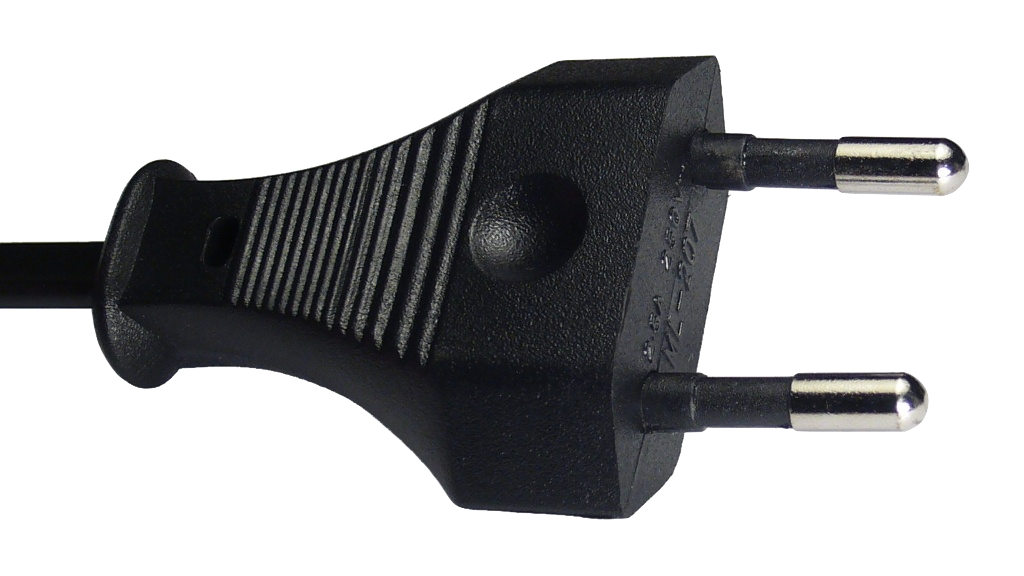
\includegraphics[width=2cm]{type_c.png}} \\
\addlinespace
I		& Matériel ayant une simple isolation mais présentant un dispositif de mise à la terre			& Ordinateur, lampadaire, fer à repasser, fer à souder\ldots		&  \multicolumn{1}{c}{\adjustbox{valign=t}{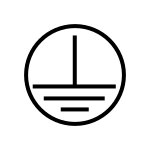
\includegraphics[width=1cm]{classe_I.png}}} & \adjustbox{valign=t}{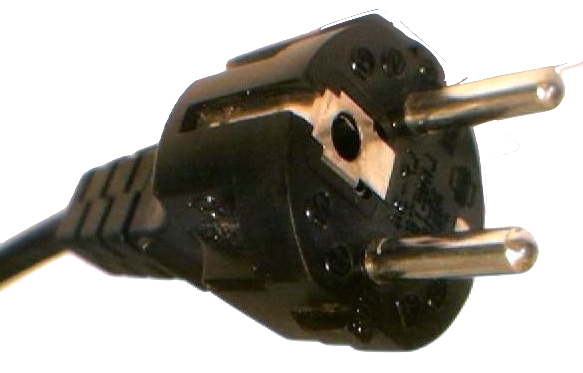
\includegraphics[width=2cm]{type_e.png}} \\
\addlinespace
II		& Matériel présentant une double isolation de la partie active \Circled{1} (isolation fonctionnelle \Circled{2} et isolation supplémentaire \Circled{3}) ne nécessitant donc pas de mise à la terre			& Chaîne hi-fi, sèche-cheveux, rasoir électrique\ldots		& \multicolumn{1}{c}{\adjustbox{valign=t}{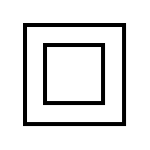
\includegraphics[width=1cm]{classe_II.png}}}		& \adjustbox{valign=t}{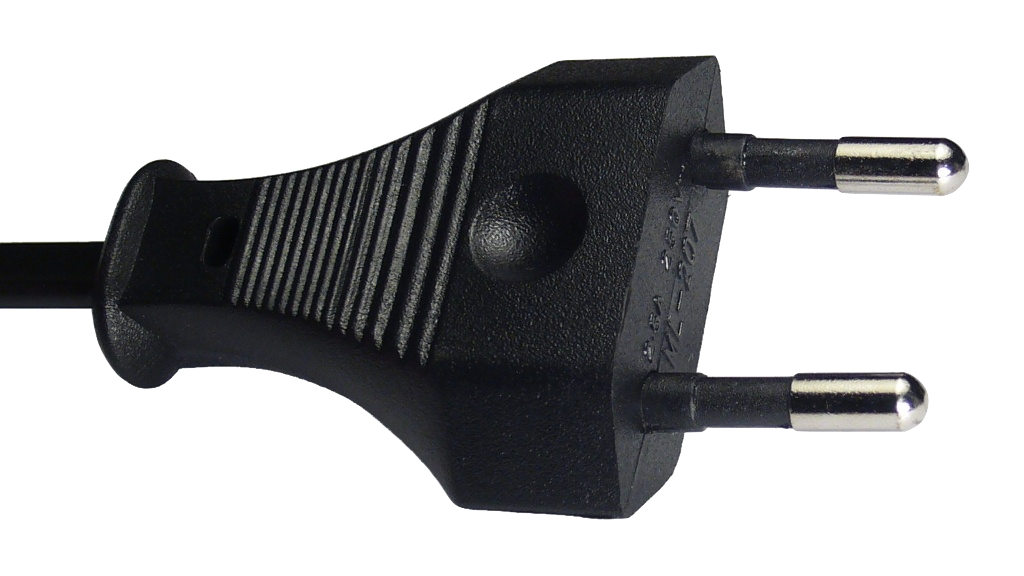
\includegraphics[width=2cm]{type_c.png}} \\
\addlinespace
III		& Matériel ne fonctionnant qu'en très basse tension (\SI{12}{\volt}	ou \SI{24}{\volt}) et ne présentant pas de dangers pour les personnes (aucune précaution particulière à prendre)			& Circuits électriques, sonnette, smartphone\ldots		& \multicolumn{1}{c}{\adjustbox{valign=t}{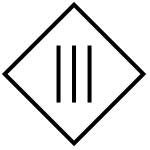
\includegraphics[width=1cm]{classe_III.png}}}		& \adjustbox{valign=t}{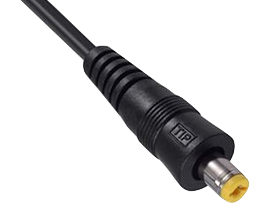
\includegraphics[width=2cm]{fiche_TBT.png}}
\end{xltabular}

\begin{figure}[h]
\caption{Matériel de classe d'isolation II} %lien éditeur Bruno Douchy : https://www.mathcha.io/editor/KxQmrUWBUm3TJwvgGohw0oEeWc2Mo9q7iLwLp4k
\tikzset{every picture/.style={line width=0.75pt}} %set default line width to 0.75pt        
\begin{tikzpicture}[x=0.75pt,y=0.75pt,yscale=-1,xscale=1]
%uncomment if require: \path (0,300); %set diagram left start at 0, and has height of 300
%Shape: Rectangle [id:dp6431615116150586] 
\draw   (120,100) -- (260,100) -- (260,160) -- (120,160) -- cycle ;
%Shape: Rectangle [id:dp21722968746615745] 
\draw   (110,90) -- (270,90) -- (270,170) -- (110,170) -- cycle ;
%Shape: Inductor [id:dp2168804832907768] 
\draw  [color={rgb, 255:red, 245; green, 166; blue, 35 }  ,draw opacity=1 ] (150,149.24) -- (150,121) .. controls (150,114.51) and (154.48,109.24) .. (160,109.24) .. controls (165.52,109.24) and (170,114.51) .. (170,121) .. controls (170,114.51) and (174.48,109.24) .. (180,109.24) .. controls (185.52,109.24) and (190,114.51) .. (190,121) .. controls (190,114.51) and (194.48,109.24) .. (200,109.24) .. controls (205.52,109.24) and (210,114.51) .. (210,121) .. controls (210,114.51) and (214.48,109.24) .. (220,109.24) .. controls (225.52,109.24) and (230,114.51) .. (230,121) -- (230,149.24) ;
%Straight Lines [id:da9190346443391305] 
\draw [color={rgb, 255:red, 245; green, 166; blue, 35 }  ,draw opacity=1 ]   (150,149.24) -- (150,180) ;
%Straight Lines [id:da1556694134502471] 
\draw [color={rgb, 255:red, 245; green, 166; blue, 35 }  ,draw opacity=1 ]   (230,149.24) -- (230,180) ;
%Straight Lines [id:da6906822080495362] 
\draw    (90,120) -- (148,120.97) ;
\draw [shift={(150,121)}, rotate = 180.95] [color={rgb, 255:red, 0; green, 0; blue, 0 }  ][line width=0.75]    (10.93,-3.29) .. controls (6.95,-1.4) and (3.31,-0.3) .. (0,0) .. controls (3.31,0.3) and (6.95,1.4) .. (10.93,3.29)   ;
%Straight Lines [id:da8500651824334423] 
\draw    (310,100) -- (272,100) ;
\draw [shift={(270,100)}, rotate = 360] [color={rgb, 255:red, 0; green, 0; blue, 0 }  ][line width=0.75]    (10.93,-3.29) .. controls (6.95,-1.4) and (3.31,-0.3) .. (0,0) .. controls (3.31,0.3) and (6.95,1.4) .. (10.93,3.29)   ;
%Straight Lines [id:da6409885852889874] 
\draw    (310,140) -- (262,140) ;
\draw [shift={(260,140)}, rotate = 360] [color={rgb, 255:red, 0; green, 0; blue, 0 }  ][line width=0.75]    (10.93,-3.29) .. controls (6.95,-1.4) and (3.31,-0.3) .. (0,0) .. controls (3.31,0.3) and (6.95,1.4) .. (10.93,3.29)   ;

% Text Node
\draw (71,112) node [anchor=north west][inner sep=0.75pt]   [align=left] {\Circled{1}};
% Text Node
\draw (318,132) node [anchor=north west][inner sep=0.75pt]   [align=left] {\Circled{2}};
% Text Node
\draw (318,91) node [anchor=north west][inner sep=0.75pt]   [align=left] {\Circled{3}};
\end{tikzpicture}
\end{figure}


\subsection{Dispositif Différentiel Résiduel\label{subsec:DDR}}

\subsubsection{Caractéristiques générales}

\begin{definition}[Dispositif Différentiel Résiduel]
Un Dispositif Différentiel Résiduel (DDR) est un appareil de protection chargé d'assurer la protection des personnes contre les défauts d'isolement provoquant potentiellement des contacts indirects (\superref{def:contact_indirect}). Son rôle est de surveiller les fuites de courant d'une installation électrique vers la terre.
\end{definition}

Il convient de bien différencier deux type de DDR :
\begin{description}
\item[Interrupteur différentiel :] protection des personnes contre les contacts indirects dont le symbole est : \\
\begin{center}


\tikzset{every picture/.style={line width=0.75pt}} %set default line width to 0.75pt        

\begin{tikzpicture}[x=0.75pt,y=0.75pt,yscale=-1,xscale=1]
%uncomment if require: \path (0,300); %set diagram left start at 0, and has height of 300

%Straight Lines [id:da2903329919565012] 
\draw    (355,127.5) -- (367.5,150) -- (367.5,170) ;
%Shape: Circle [id:dp3187615529298826] 
\draw   (369.5,130) .. controls (369.5,128.9) and (368.6,128) .. (367.5,128) .. controls (366.4,128) and (365.5,128.9) .. (365.5,130) .. controls (365.5,131.1) and (366.4,132) .. (367.5,132) .. controls (368.6,132) and (369.5,131.1) .. (369.5,130) -- cycle ;
%Straight Lines [id:da6291068913098858] 
\draw    (367.5,128) -- (367.5,120) ;
%Rounded Rect [id:dp5228947876486602] 
\draw   (362.5,160) .. controls (362.5,158.62) and (363.62,157.5) .. (365,157.5) -- (390,157.5) .. controls (391.38,157.5) and (392.5,158.62) .. (392.5,160) -- (392.5,160) .. controls (392.5,161.38) and (391.38,162.5) .. (390,162.5) -- (365,162.5) .. controls (363.62,162.5) and (362.5,161.38) .. (362.5,160) -- cycle ;
%Straight Lines [id:da9535405775656056] 
\draw  [dash pattern={on 4.5pt off 4.5pt}]  (382.25,139.75) -- (357.5,140) -- (357.5,160) -- (362.5,160) ;
%Straight Lines [id:da293136389225495] 
\draw    (375,127.5) -- (387.5,150) -- (387.5,170) ;
%Shape: Circle [id:dp1387355280779735] 
\draw   (389.5,130) .. controls (389.5,128.9) and (388.6,128) .. (387.5,128) .. controls (386.4,128) and (385.5,128.9) .. (385.5,130) .. controls (385.5,131.1) and (386.4,132) .. (387.5,132) .. controls (388.6,132) and (389.5,131.1) .. (389.5,130) -- cycle ;
%Straight Lines [id:da810942314060853] 
\draw    (387.5,128) -- (387.5,120) ;

\end{tikzpicture}
\end{center}

\item[Disjoncteur différentiel :] protection des personnes contre les contacts indirects et protection des circuits contre les surintensités et les court-circuits dont le symbole est : \\
\begin{center}


\tikzset{every picture/.style={line width=0.75pt}} %set default line width to 0.75pt        

\begin{tikzpicture}[x=0.75pt,y=0.75pt,yscale=-1,xscale=1]
%uncomment if require: \path (0,300); %set diagram left start at 0, and has height of 300

%Straight Lines [id:da26208223112851936] 
\draw    (527.5,100) -- (540,122.5) -- (540,142.5) ;
%Straight Lines [id:da5822281275248988] 
\draw    (540,102.5) -- (540,92.5) ;
%Rounded Rect [id:dp41055324766610257] 
\draw   (535,132.5) .. controls (535,131.12) and (536.12,130) .. (537.5,130) -- (562.5,130) .. controls (563.88,130) and (565,131.12) .. (565,132.5) -- (565,132.5) .. controls (565,133.88) and (563.88,135) .. (562.5,135) -- (537.5,135) .. controls (536.12,135) and (535,133.88) .. (535,132.5) -- cycle ;
%Straight Lines [id:da30592283799275743] 
\draw  [dash pattern={on 4.5pt off 4.5pt}]  (554.75,112.25) -- (530,112.5) -- (530,132.5) -- (535,132.5) ;
%Straight Lines [id:da7841914077845515] 
\draw    (538,100.5) -- (542,104.5) ;
%Straight Lines [id:da01685582709758693] 
\draw    (542,100.5) -- (538,104.5) ;

%Straight Lines [id:da7197353055881572] 
\draw    (547.5,100) -- (560,122.5) -- (560,142.5) ;
%Straight Lines [id:da316262731013633] 
\draw    (560,102.5) -- (560,92.5) ;
%Straight Lines [id:da6806510311797901] 
\draw    (558,100.5) -- (562,104.5) ;
%Straight Lines [id:da5532087619463947] 
\draw    (562,100.5) -- (558,104.5) ;






\end{tikzpicture}

\end{center}
\end{description}

\begin{table}[h]
\caption{Valeur du seuil de $I_{\Delta n}$ fonction de $R_{A}$ et $U_{L}$}
\begin{tabularx}{\linewidth}{C i k S C i k S C i k S}
\toprule
\thead{$U_{L}$}	& \multicolumn{2}{c}{\thead{$R_{A}$ (\si{\ohm})}}	& 	{$I_{\Delta n}$ (\si{\ampere})}	& \thead{$U_{L}$}	& \multicolumn{2}{c}{\thead{$R_{A}$ (\si{\ohm})}}	& 	{$I_{\Delta n}$ (\si{\ampere})} & \thead{$U_{L}$}	& \multicolumn{2}{c}{\thead{$R_{A}$ (\si{\ohm})}}	& 	{$I_{\Delta n}$ (\si{\ampere})}	\\
\midrule
\SI{50}{\volt}	& \geq & 1660	&  0,030 		& \SI{25}{\volt}	& \geq & 500	& 	0,030	& \SI{12}{\volt}		& \geq & 400	&  0,030 \\
						& \geq & 166		&  0,300 		& 							& \geq & 83	&  0,300 	& 								& \geq & 40	&  0,300  \\
						& \geq & 100		&  0,500 		& 							& \geq & 50	&  0,500 	& 								& \geq & 24	&  0,500  \\
						& \geq & 16		&  3				& 							& \geq & 8		& 		 3 		& 								& \geq & 4		&  3  \\
\bottomrule
\end{tabularx}
\end{table}

\subsubsection{Marquage normalisé}

Comme tout appareil de protection, le DDR respecte des normes de qualité strictes (Conformité Européenne) et doivent présenter plusieurs marquages réglementaires, ainsi qu'un bouton \og TEST \fg{} pour informer l'installateur et l'utilisateur des caractéristiques du DDR. Cela informe de la conformité de l'appareil de protection.
\startcstep %remet les compteurs des légendes en pastille à zéro
\begin{center}
\begin{figure}[h]
\caption{Marquage d'un interrupteur différentiel}
\begin{subfigure}[t]{0.49\linewidth}
\subcaption{Vue de dessus}
\begin{annotate}
{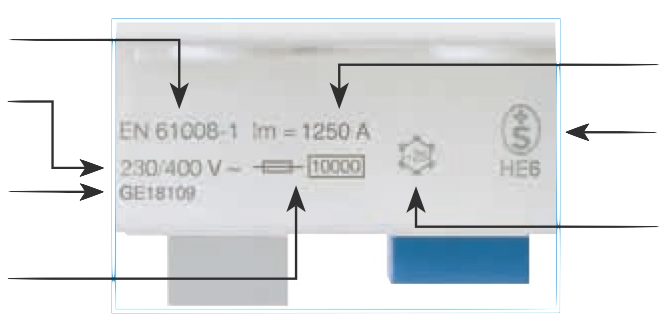
\includegraphics[scale=1]{DDR_dessus}}{0.25}
%\helpgrid[gray] 
\node at (-11.8,4.3) {\Circled{1}};
\node at (-11.8,2.2) {\Circled{2}};
\node at (-11.8,-0.85) {\Circled{3}};
\node at (-11.8,-3.85) {\Circled{4}};
\node at (11.7,3.4) {\Circled{5}};
\node at (11.7,1.1) {\Circled{6}};
\node at (11.7,-2.1) {\Circled{7}};
\end{annotate} 
\end{subfigure}
\begin{subfigure}[t]{0.49\linewidth}
\subcaption{Vue de dessus}
\begin{annotate}
{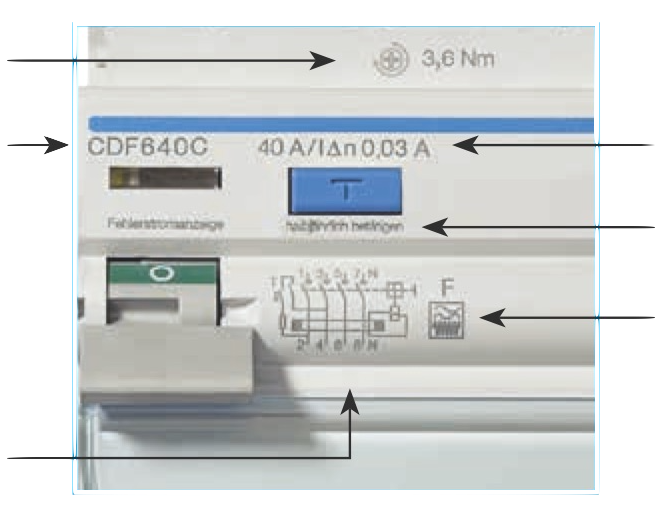
\includegraphics[scale=1]{DDR_avant}}{0.25}
%\helpgrid[gray] 
\node at (-11.8,6.7) {\Circled{8}};
\node at (-11.8,3.8) {\Circled{9}};
\node at (-11.9,-6.85) {\Circled{10}};
\node at (11.7,3.85) {\Circled{11}};
\node at (11.7,1) {\Circled{12}};
\node at (11.7,-2.05) {\Circled{13}};
\end{annotate} 
\end{subfigure}
\end{figure}
\end{center}
\begin{minipage}{\linewidth} %usage d'un environnement mini-page pour éviter les décalage au début de la première colonne quand l'élément n'est pas du texte simple
	\begin{multicols}{2} %répartition du texte dans l'environnement en deux colonnes
		\Circled{1} norme du produit\\ %légende automatique
		\Circled{2} tension assignée $230/400\si{\volt}\sim$\\
		\Circled{3} code de production\\
		\Circled{4} signe \og Courant assigné de court-circuit \SI{10000}{\ampere} \fg{} en combinaison avec un fusible en amont \\
		\Circled{5} pouvoir assigné de coupure \og \SI{1250}{\ampere} \fg{} \\
		\Circled{6} signe de sécurité ESTI (équivalent de la norme NF pour la Suisse) \\
		\Circled{7} signe \og Flocon de neige \fg{} (utilisation pour une température ambiante jusqu'à \SI{-25}{\degree}) \\
		\columnbreak\\ %passage à la deuxième colonne
		\Circled{8} couple de serrage \si{\newton\meter} \\
		\Circled{9} désignation du type\\
		\Circled{10} schéma des connexions\\
		\Circled{11} courant assigné $I_n$ de \SI{40}{\ampere} et calibre du DDR $I_{\Delta n}$\\
		\Circled{12} note concernant le test \og à effectuer tous les six mois \fg{}\\
		 \Circled{13} type de courant différentiel (type F)
	\end{multicols}
\end{minipage}


\subsubsection{Composante du courant de défaut}

Les DDR peuvent détecter plusieurs composantes du courant de défaut. C'est un paramètre qui peut varier selon le type d'appareil électrique protégé par le DDR.

%--------------------------------------
%ELECTROTECHNIQUE - SCHEMA DE LIAISON A LA TERRE
%--------------------------------------

%utiliser les environnement \begin{comment} \end{comment} pour mettre en commentaire le préambule une fois la programmation appelée dans le document maître (!ne pas oublier de mettre en commentaire \end{document}!)

\begin{comment}

\documentclass[a4paper, 11pt, twoside, fleqn]{memoir}

\usepackage{AOCDTF}

\marqueurchapitre

%lien d'édition des figures Tikz sur le site mathcha.io (rajouter le lien d'une modification effectuée sur la figure tikz avec le nom du modificateur car il n'y a qu'un lien par compte)

%lien éditeur Bruno Douchy : https://www.mathcha.io/editor/zjygnFElSdyhJ72e3zT5ZgqwBT4DKnovswpXn1q

%--------------------------------------
%corps du document
%--------------------------------------

\begin{document} %corps du document
	\openleft %début de chapitre à gauche

\end{comment}

\begin{xltabular}{\textwidth}{l c >{\compress}X c c }
\caption{Différents types de DDR selon les composantes du courant de défaut}\\
\toprule
\thead{Type}		& \thead{Symbole}		& \thead{Caractéristiques}	& \thead{Forme d'onde}		& \thead{Type de charge} \\
\midrule
\endfirsthead %en-tête de la première page du tableau  
\multicolumn{5}{l}{\small\textit{Page précédente}} \\
\midrule %filet de milieu de tableau
\thead{Type}		& \thead{Symbole}		& \thead{Caractéristiques}	& \thead{Forme d'onde}		& \thead{Type de charge} \\
\midrule
\endhead
\midrule %filet de milieu de tableau
\multicolumn{5}{r}{\small\textit{Page suivante}} \\
\endfoot %pied de page de toutes les pages du tableau
\bottomrule
\endlastfoot %pied de page de la dernièredu tableau
Type AC		& \adjustbox{valign=t}{
\includegraphics[height=0.4cm]{type_ac.png}}		& 
\begin{tabitemize}
\item détection des courants alternatifs différentiels\,;
\item utilisation courante en domestique couvrant la plupart des besoin.
\end{tabitemize}
&

\adjustbox{valign=t}{

\tikzset{every picture/.style={line width=0.75pt}} %set default line width to 0.75pt        

\begin{tikzpicture}[x=0.75pt,y=0.75pt,yscale=-1,xscale=1]
%uncomment if require: \path (0,57); %set diagram left start at 0, and has height of 57

%Straight Lines [id:da2943661507092279] 
\draw    (7.5,25) -- (78,25) ;
\draw [shift={(80,25)}, rotate = 180] [color={rgb, 255:red, 0; green, 0; blue, 0 }  ][line width=0.75]    (10.93,-3.29) .. controls (6.95,-1.4) and (3.31,-0.3) .. (0,0) .. controls (3.31,0.3) and (6.95,1.4) .. (10.93,3.29)   ;
%Shape: Wave [id:dp24323544196681968] 
\draw  [color={rgb, 255:red, 126; green, 211; blue, 33 }  ,draw opacity=1 ] (15,25) .. controls (19.08,14.75) and (22.98,5) .. (27.5,5) .. controls (32.02,5) and (35.92,14.75) .. (40,25) .. controls (44.08,35.25) and (47.98,45) .. (52.5,45) .. controls (57.02,45) and (60.92,35.25) .. (65,25) ;
%Straight Lines [id:da09599799976641754] 
\draw    (7.5,25) -- (30,25) ;
%Straight Lines [id:da7289357219255289] 
\draw    (43.75,25) -- (66.25,25) ;


\end{tikzpicture}}
 &
 
\adjustbox{valign=t}{


\tikzset{every picture/.style={line width=0.75pt}} %set default line width to 0.75pt        

\begin{tikzpicture}[x=0.75pt,y=0.75pt,yscale=-1,xscale=1]
%uncomment if require: \path (0,98); %set diagram left start at 0, and has height of 98

%Straight Lines [id:da7324284340679806] 
\draw    (122.5,17.5) -- (127.5,17.5) ;
%Shape: Rectangle [id:dp18713096911447358] 
\draw   (92.5,12.5) -- (122.5,12.5) -- (122.5,22.5) -- (92.5,22.5) -- cycle ;
%Straight Lines [id:da2214074924221885] 
\draw    (87.5,17.5) -- (92.5,17.5) ;

%Straight Lines [id:da09102665939260723] 
\draw    (107.5,25) -- (102.5,45) -- (112.5,37.5) -- (108.23,54.59) ;
\draw [shift={(107.5,57.5)}, rotate = 284.04] [fill={rgb, 255:red, 0; green, 0; blue, 0 }  ][line width=0.08]  [draw opacity=0] (5.36,-2.57) -- (0,0) -- (5.36,2.57) -- cycle    ;

% Text Node
\draw (81.5,61) node [anchor=north west][inner sep=0.75pt]   [align=left] {linéaire};


\end{tikzpicture}}

  \\
    \addlinespace
  \addlinespace

  
  
  Type A		& \adjustbox{valign=t}{
\includegraphics[height=0.4cm]{type_a.png}}		& 
\begin{tabitemize}
\item détection des courants différentiels alternatifs et des courants différentiels continus pulsés\,;
\item utilisation spécifique pour les charges électriques monophasées de type 1.
\end{tabitemize}
&

\adjustbox{valign=t}{




\tikzset{every picture/.style={line width=0.75pt}} %set default line width to 0.75pt        

\begin{tikzpicture}[x=0.75pt,y=0.75pt,yscale=-1,xscale=1]
%uncomment if require: \path (0,108); %set diagram left start at 0, and has height of 108

%Shape: Wave [id:dp27700594343461393] 
\draw  [color={rgb, 255:red, 126; green, 211; blue, 33 }  ,draw opacity=1 ] (35,45) .. controls (39.08,34.75) and (42.98,25) .. (47.5,25) .. controls (52.02,25) and (55.92,34.75) .. (60,45) .. controls (64.08,55.25) and (67.98,65) .. (72.5,65) .. controls (77.02,65) and (80.92,55.25) .. (85,45) .. controls (89.08,34.75) and (92.98,25) .. (97.5,25) .. controls (102.02,25) and (105.92,34.75) .. (110,45) ;
%Straight Lines [id:da5910455205676639] 
\draw    (23.75,45) -- (123,45) ;
\draw [shift={(125,45)}, rotate = 180] [color={rgb, 255:red, 0; green, 0; blue, 0 }  ][line width=0.75]    (10.93,-3.29) .. controls (6.95,-1.4) and (3.31,-0.3) .. (0,0) .. controls (3.31,0.3) and (6.95,1.4) .. (10.93,3.29)   ;
%Straight Lines [id:da5095890041059973] 
\draw [color={rgb, 255:red, 126; green, 211; blue, 33 }  ,draw opacity=1 ]   (60,45) -- (85,45) ;
%Shape: Trapezoid [id:dp9576415302257589] 
\draw  [color={rgb, 255:red, 126; green, 211; blue, 33 }  ,draw opacity=1 ] (85,45) -- (84.7,46) -- (60.3,46) -- (60,45) -- cycle ;
%Shape: Rectangle [id:dp7690910497329457] 
\draw  [draw opacity=0][fill={rgb, 255:red, 255; green, 255; blue, 255 }  ,fill opacity=1 ][line width=5.25]  (35,45.5) -- (105,45.5) -- (105,68) -- (35,68) -- cycle ;




\end{tikzpicture}

}
 &
 
 
\adjustbox{valign=t}{



\tikzset{every picture/.style={line width=0.75pt}} %set default line width to 0.75pt        

\begin{tikzpicture}[x=0.75pt,y=0.75pt,yscale=-1,xscale=1]
%uncomment if require: \path (0,152); %set diagram left start at 0, and has height of 152

%Straight Lines [id:da2993135281874989] 
\draw    (40,35) -- (30,15) ;
%Straight Lines [id:da1407255659834652] 
\draw    (35,35) -- (25,15) ;
%Straight Lines [id:da0646281171352201] 
\draw    (42.5,25) -- (22.5,25) ;
%Shape: Square [id:dp8095195384599084] 
\draw   (42.5,5) -- (82.5,5) -- (82.5,45) -- (42.5,45) -- cycle ;
%Shape: Boxed Line [id:dp9015036881777688] 
\draw    (73.5,15) -- (73.5,35) ;
%Shape: Triangle [id:dp25930553779074683] 
\draw   (72.5,25) -- (52.5,35) -- (52.5,15) -- cycle ;
%Straight Lines [id:da624315601423471] 
\draw    (62.5,50) -- (57.5,70) -- (67.5,62.5) -- (63.23,79.59) ;
\draw [shift={(62.5,82.5)}, rotate = 284.04] [fill={rgb, 255:red, 0; green, 0; blue, 0 }  ][line width=0.08]  [draw opacity=0] (5.36,-2.57) -- (0,0) -- (5.36,2.57) -- cycle    ;
%Straight Lines [id:da583175718122269] 
\draw    (102.5,25) -- (82.5,25) ;

% Text Node
\draw (17.5,87) node [anchor=north west][inner sep=0.75pt]   [align=left] {\begin{minipage}[lt]{61.699375pt}\setlength\topsep{0pt}
\begin{center}
redressée\\monophasée
\end{center}

\end{minipage}};


\end{tikzpicture}
}

  \\
    \addlinespace
  \addlinespace

  
    Type F		& \adjustbox{valign=t}{
\includegraphics[height=0.4cm]{type_f.png}}		& 
\begin{tabitemize}
\item détection des courants différentiels alternatifs, les courants différentiels continus pulsés et les courants différentiels de fréquences mixtes jusqu'à \SI{1}{\kilo\hertz}\,;
\item utilisation spécifique pour circuits comportant des variateurs de vitesse monophasés.
\end{tabitemize}
&

\adjustbox{valign=t}{
\tikzset{every picture/.style={line width=0.75pt}} %set default line width to 0.75pt        

\begin{tikzpicture}[x=0.75pt,y=0.75pt,yscale=-1,xscale=1]
%uncomment if require: \path (0,108); %set diagram left start at 0, and has height of 108

%Straight Lines [id:da8344481258673822] 
\draw [color={rgb, 255:red, 126; green, 211; blue, 33 }  ,draw opacity=1 ]   (47.5,25) -- (47.5,45) ;
%Straight Lines [id:da45734535299498047] 
\draw [color={rgb, 255:red, 126; green, 211; blue, 33 }  ,draw opacity=1 ]   (45,26) -- (45,45) ;
%Straight Lines [id:da4148698837495829] 
\draw [color={rgb, 255:red, 126; green, 211; blue, 33 }  ,draw opacity=1 ]   (42.5,28.5) -- (42.5,44.5) ;
%Straight Lines [id:da9637733631041641] 
\draw [color={rgb, 255:red, 126; green, 211; blue, 33 }  ,draw opacity=1 ]   (37.5,39) -- (37.5,45) ;
%Straight Lines [id:da15505371109761856] 
\draw [color={rgb, 255:red, 126; green, 211; blue, 33 }  ,draw opacity=1 ]   (40,33.5) -- (40,44.5) ;
%Straight Lines [id:da8124028319543418] 
\draw [color={rgb, 255:red, 126; green, 211; blue, 33 }  ,draw opacity=1 ]   (52.5,29) -- (52.5,45) ;
%Straight Lines [id:da9805020896518191] 
\draw [color={rgb, 255:red, 126; green, 211; blue, 33 }  ,draw opacity=1 ]   (50,26) -- (50,45) ;
%Straight Lines [id:da4116431840997269] 
\draw [color={rgb, 255:red, 126; green, 211; blue, 33 }  ,draw opacity=1 ]   (55,34) -- (55,45) ;
%Straight Lines [id:da8823890585871352] 
\draw [color={rgb, 255:red, 126; green, 211; blue, 33 }  ,draw opacity=1 ]   (57.5,39) -- (57.5,45) ;
%Straight Lines [id:da9104778326348498] 
\draw [color={rgb, 255:red, 126; green, 211; blue, 33 }  ,draw opacity=1 ]   (72.5,65) -- (72.5,45) ;
%Straight Lines [id:da36879417192210706] 
\draw [color={rgb, 255:red, 126; green, 211; blue, 33 }  ,draw opacity=1 ]   (75,64) -- (75,45) ;
%Straight Lines [id:da056894793071553984] 
\draw [color={rgb, 255:red, 126; green, 211; blue, 33 }  ,draw opacity=1 ]   (77.5,61.5) -- (77.5,45.5) ;
%Straight Lines [id:da926320044180968] 
\draw [color={rgb, 255:red, 126; green, 211; blue, 33 }  ,draw opacity=1 ]   (82.5,51) -- (82.5,45) ;
%Straight Lines [id:da4802255081072313] 
\draw [color={rgb, 255:red, 126; green, 211; blue, 33 }  ,draw opacity=1 ]   (80,56.5) -- (80,45.5) ;
%Straight Lines [id:da8191961490083182] 
\draw [color={rgb, 255:red, 126; green, 211; blue, 33 }  ,draw opacity=1 ]   (67.5,61) -- (67.5,45) ;
%Straight Lines [id:da2923358818287347] 
\draw [color={rgb, 255:red, 126; green, 211; blue, 33 }  ,draw opacity=1 ]   (70,64) -- (70,45) ;
%Straight Lines [id:da3136693713803336] 
\draw [color={rgb, 255:red, 126; green, 211; blue, 33 }  ,draw opacity=1 ]   (65,56) -- (65,45) ;
%Straight Lines [id:da549046744886196] 
\draw [color={rgb, 255:red, 126; green, 211; blue, 33 }  ,draw opacity=1 ]   (62.5,51) -- (62.5,45) ;

%Shape: Wave [id:dp9341521104203707] 
\draw  [color={rgb, 255:red, 0; green, 0; blue, 0 }  ,draw opacity=1 ] (35,45) .. controls (39.08,34.75) and (42.98,25) .. (47.5,25) .. controls (52.02,25) and (55.92,34.75) .. (60,45) .. controls (64.08,55.25) and (67.98,65) .. (72.5,65) .. controls (77.02,65) and (80.92,55.25) .. (85,45) ;
%Straight Lines [id:da8093364598636541] 
\draw    (27.5,45) -- (98,45) ;
\draw [shift={(100,45)}, rotate = 180] [color={rgb, 255:red, 0; green, 0; blue, 0 }  ][line width=0.75]    (10.93,-3.29) .. controls (6.95,-1.4) and (3.31,-0.3) .. (0,0) .. controls (3.31,0.3) and (6.95,1.4) .. (10.93,3.29)   ;




\end{tikzpicture}

}
 &
 
 
\adjustbox{valign=t}{


\tikzset{every picture/.style={line width=0.75pt}} %set default line width to 0.75pt        

\begin{tikzpicture}[x=0.75pt,y=0.75pt,yscale=-1,xscale=1]
%uncomment if require: \path (0,152); %set diagram left start at 0, and has height of 152

%Straight Lines [id:da2004774518549749] 
\draw    (40,35) -- (30,15) ;
%Straight Lines [id:da28878490688185077] 
\draw    (35,35) -- (25,15) ;
%Straight Lines [id:da28622017833538005] 
\draw    (42.5,25) -- (22.5,25) ;
%Straight Lines [id:da27361779183994883] 
\draw    (62.5,50) -- (57.5,70) -- (67.5,62.5) -- (63.23,79.59) ;
\draw [shift={(62.5,82.5)}, rotate = 284.04] [fill={rgb, 255:red, 0; green, 0; blue, 0 }  ][line width=0.08]  [draw opacity=0] (5.36,-2.57) -- (0,0) -- (5.36,2.57) -- cycle    ;
%Straight Lines [id:da3667194527320474] 
\draw    (102.5,25) -- (82.5,25) ;
%Shape: Square [id:dp27983484657325586] 
\draw   (42.5,5) -- (82.5,5) -- (82.5,45) -- (42.5,45) -- cycle ;
%Shape: Boxed Line [id:dp856307990834614] 
\draw    (52.5,15) -- (52.5,35) ;
%Straight Lines [id:da34232786335443943] 
\draw    (72.5,15) -- (56.5,25) -- (69.96,33.41) ;
\draw [shift={(72.5,35)}, rotate = 212.01] [fill={rgb, 255:red, 0; green, 0; blue, 0 }  ][line width=0.08]  [draw opacity=0] (5.36,-2.57) -- (0,0) -- (5.36,2.57) -- cycle    ;
%Shape: Boxed Line [id:dp1790472061066909] 
\draw    (55.5,15) -- (55.5,35) ;


% Text Node
\draw (18.5,87) node [anchor=north west][inner sep=0.75pt]   [align=left] {\begin{minipage}[lt]{61.699375pt}\setlength\topsep{0pt}
\begin{center}
convertie\\monophasée
\end{center}

\end{minipage}};


\end{tikzpicture}

}

  \\
    \addlinespace
        \addlinespace


      Type B		& \adjustbox{valign=t}{
\includegraphics[height=0.4cm]{type_b.png}}		& 
\begin{tabitemize}
\item détection des courants différentiels alternatifs, les courants différentiels continus pulsés, des courants différentiels de fréquences mixtes jusqu'à \SI{1}{\kilo\hertz} et des courants différentiels continus lisses\,;
\item utilisation spécifique pour circuits comportant des variateurs de vitesse triphasés, un système photovoltaïque, une borne de recharge de véhicule électrique ou encore des équipements médicaux.
\end{tabitemize}
&

\adjustbox{valign=t}{


\tikzset{every picture/.style={line width=0.75pt}} %set default line width to 0.75pt        

\begin{tikzpicture}[x=0.75pt,y=0.75pt,yscale=-1,xscale=1]
%uncomment if require: \path (0,108); %set diagram left start at 0, and has height of 108

%Straight Lines [id:da7026343722095999] 
\draw    (47.5,87.5) -- (143,87.5) ;
\draw [shift={(145,87.5)}, rotate = 180] [color={rgb, 255:red, 0; green, 0; blue, 0 }  ][line width=0.75]    (10.93,-3.29) .. controls (6.95,-1.4) and (3.31,-0.3) .. (0,0) .. controls (3.31,0.3) and (6.95,1.4) .. (10.93,3.29)   ;
%Shape: Parabola [id:dp4469234992699831] 
\draw  [color={rgb, 255:red, 126; green, 211; blue, 33 }  ,draw opacity=1 ] (69.58,75) .. controls (65.55,65) and (61.52,65) .. (57.5,75) ;
%Shape: Parabola [id:dp10691023078597706] 
\draw  [color={rgb, 255:red, 126; green, 211; blue, 33 }  ,draw opacity=1 ] (81.67,75) .. controls (77.64,65) and (73.61,65) .. (69.58,75) ;
%Shape: Parabola [id:dp9540942461898068] 
\draw  [color={rgb, 255:red, 126; green, 211; blue, 33 }  ,draw opacity=1 ] (93.75,75) .. controls (89.73,65) and (85.7,65) .. (81.67,75) ;
%Shape: Parabola [id:dp6220203064360257] 
\draw  [color={rgb, 255:red, 126; green, 211; blue, 33 }  ,draw opacity=1 ] (105.83,75) .. controls (101.8,65) and (97.77,65) .. (93.75,75) ;
%Shape: Parabola [id:dp4992966008122459] 
\draw  [color={rgb, 255:red, 126; green, 211; blue, 33 }  ,draw opacity=1 ] (117.92,75) .. controls (113.89,65) and (109.86,65) .. (105.83,75) ;
%Shape: Parabola [id:dp01154198803526707] 
\draw  [color={rgb, 255:red, 126; green, 211; blue, 33 }  ,draw opacity=1 ] (130,75) .. controls (125.98,65) and (121.95,65) .. (117.92,75) ;




\end{tikzpicture}

}
 &
 
 
\adjustbox{valign=t}{


\tikzset{every picture/.style={line width=0.75pt}} %set default line width to 0.75pt        

\begin{tikzpicture}[x=0.75pt,y=0.75pt,yscale=-1,xscale=1]
%uncomment if require: \path (0,141); %set diagram left start at 0, and has height of 141

%Straight Lines [id:da4147930693711671] 
\draw    (60,42.5) -- (50,22.5) ;
%Straight Lines [id:da7913487771488718] 
\draw    (55,42.5) -- (45,22.5) ;
%Straight Lines [id:da12782809797617567] 
\draw    (62.5,32.5) -- (37.5,32.5) ;
%Shape: Square [id:dp3051019253176962] 
\draw   (62.5,12) -- (102.5,12) -- (102.5,52) -- (62.5,52) -- cycle ;
%Shape: Boxed Line [id:dp3719227311734635] 
\draw    (93.5,22) -- (93.5,42) ;
%Shape: Triangle [id:dp5734231710257448] 
\draw   (92.5,32) -- (72.5,42) -- (72.5,22) -- cycle ;
%Straight Lines [id:da20189459286959577] 
\draw    (82.5,57) -- (77.5,77) -- (87.5,69.5) -- (83.23,86.59) ;
\draw [shift={(82.5,89.5)}, rotate = 284.04] [fill={rgb, 255:red, 0; green, 0; blue, 0 }  ][line width=0.08]  [draw opacity=0] (5.36,-2.57) -- (0,0) -- (5.36,2.57) -- cycle    ;
%Straight Lines [id:da8309944422064088] 
\draw    (122.5,32) -- (102.5,32) ;
%Straight Lines [id:da522665354082454] 
\draw    (50,42.5) -- (40,22.5) ;

% Text Node
\draw (47.5,94.5) node [anchor=north west][inner sep=0.75pt]   [align=left] {\begin{minipage}[lt]{48.078125pt}\setlength\topsep{0pt}
\begin{center}
redressée\\triphasée
\end{center}

\end{minipage}};


\end{tikzpicture}


}

  \\
  
\end{xltabular}


%\end{document}



\subsubsection{Principe de fonctionnement\label{subsubsec:principe_fonctionnement_ddr}}

Les éléments essentiels d'un DDR sont les suivants : \\
\begin{minipage}{\linewidth} %usage d'un environnement mini-page pour éviter les décalage au début de la première colonne quand l'élément n'est pas du texte simple
	\begin{multicols}{2} %répartition du texte dans l'environnement en deux colonnes
	\startcstep %remet les compteurs des légendes en pastille à zéro
		\Circled{1} bouton test d'essai du DDR\\ %légende automatique
		\Circled{2} transformateur d'intensité (tore de détection)\\
		\Circled{3} relais de déclenchement  \\
		\Circled{4} mécanisme à déclenchement libre sans retour automatique \\
		\columnbreak\\ %passage à la deuxième colonne
		$I_1$ : courant \og d'arrivée \fg{} du récepteur \\
		$I_2$ : courant \og de sortie \fg{} du récepteur \\
		$I_d$ : courant de défaut\\
		$I_c$ : courant de contact\\
		$R_B$ : résistance de terre du neutre\\
		$R_A$ : résistance de la prise de terre de l'installation électrique 
	\end{multicols}
\end{minipage}
~\\
Pour le fonctionnement d'un DDR, les conditions suivantes doivent être remplie :
\begin{itemize}
\item le point neutre du transformateur HT/BT doit être mis à la terre\,;
\item aucune liaison entre le conducteur de neutre et le conducteur de protection ne doit être réalisée en aval du DDR\,;
\item le conducteur de protection ne doit pas transiter dans le transformateur d'intensité\,;
\item le réseau doit être alternatif.
\end{itemize}

%--------------------------------------
%ELECTROTECHNIQUE - SCHEMA DE LIAISON A LA TERRE
%--------------------------------------

%utiliser les environnement \begin{comment} \end{comment} pour mettre en commentaire le préambule une fois la programmation appelée dans le document maître (!ne pas oublier de mettre en commentaire \end{document}!)

\begin{comment}

\documentclass[a4paper, 11pt, twoside, fleqn]{memoir}

\usepackage{AOCDTF}

%--------------------------------------
%CANEVAS
%--------------------------------------

\newcommand\BoxColor{\ifcase\thechapshift blue!30\or brown!30\or pink!30\or cyan!30\or green!30\or teal!30\or purple!30\or red!30\or olive!30\or orange!30\or lime!30\or gray!\or magenta!30\else yellow!30\fi} %définition de la couleur des marqueurs de chapitre

\newcounter{chapshift} %compteur de chapitre du marqueur de chapitre
\addtocounter{chapshift}{-1}
	
\newif\ifFrame %instruction conditionnelle pour les couleurs des pages
\Frametrue

\pagestyle{plain}

% the main command; the mandatory argument sets the color of the vertical box
\newcommand\ChapFrame{%
\AddEverypageHook{%
\ifFrame
\ifthenelse{\isodd{\value{page}}}
  {\backgroundsetup{contents={%
  \begin{tikzpicture}[overlay,remember picture]
  \node[
  	rounded corners=3pt,
    fill=\BoxColor,
    inner sep=0pt,
    rectangle,
    text width=1.5cm,
    text height=5.5cm,
    align=center,
    anchor=north west
  ] 
  at ($ (current page.north west) + (-0cm,-2*\thechapshift cm) $) %nombre négatif = espacement des marqueurs entre les différents chapitres (à régler en fin de rédaction) (4.5cm vaut un espacement équivalement à la hauteur du marqueur, une page peut en contenir 6 avec cet espacement-la mais il est le plus équilibré)
    {\rotatebox{90}{\hspace*{.5cm}%
      \parbox[c][1.2cm][t]{5cm}{%
        \raggedright\textcolor{black}{\sffamily\textbf{\leftmark}}}}};
  \end{tikzpicture}}}
  }
  {\backgroundsetup{contents={%
  \begin{tikzpicture}[overlay,remember picture]
  \node[
  	rounded corners=3pt,
    fill=\BoxColor,
    inner sep=0pt,
    rectangle,
    text width=1.5cm,
    text height=5.5cm,
    align=center,
    anchor=north east
  ] 
  at ($ (current page.north east) + (-0cm,-2*\thechapshift cm) $) %nombre négatif = espacement des marqueurs entre les différents chapitres (à régler en fin de rédaction) (4.5cm vaut un espacement équivalement à la hauteur du marqueur, une page peut en contenir 6 avec cet espacement-la mais il est le plus équilibré)
    {\rotatebox{90}{\hspace*{.5cm}%
      \parbox[c][1.2cm][t]{5cm}{%
        \raggedright\textcolor{black}{\sffamily\textbf{\leftmark}}}}};
  \end{tikzpicture}}}%
  }
  \BgMaterial%
  \fi%
}%
  \stepcounter{chapshift}
}

\renewcommand\chaptermark[1]{\markboth{\thechapter.~#1}{}} %redéfinition du marqueur de chapitre pour ne contenir que le titre du chapitre %à personnaliser selon le nombre de chapitre dans le cours

%--------------------------------------
%corps du document
%--------------------------------------

\begin{document} %corps du document
	\openleft %début de chapitre à gauche

\end{comment}

\begin{figure}[h]
\caption{Principe de fonctionnement d'un DDR}



% Pattern Info
 
\tikzset{
pattern size/.store in=\mcSize, 
pattern size = 5pt,
pattern thickness/.store in=\mcThickness, 
pattern thickness = 0.3pt,
pattern radius/.store in=\mcRadius, 
pattern radius = 1pt}
\makeatletter
\pgfutil@ifundefined{pgf@pattern@name@_uf0m8v139}{
\pgfdeclarepatternformonly[\mcThickness,\mcSize]{_uf0m8v139}
{\pgfqpoint{0pt}{0pt}}
{\pgfpoint{\mcSize+\mcThickness}{\mcSize+\mcThickness}}
{\pgfpoint{\mcSize}{\mcSize}}
{
\pgfsetcolor{\tikz@pattern@color}
\pgfsetlinewidth{\mcThickness}
\pgfpathmoveto{\pgfqpoint{0pt}{0pt}}
\pgfpathlineto{\pgfpoint{\mcSize+\mcThickness}{\mcSize+\mcThickness}}
\pgfusepath{stroke}
}}
\makeatother
\tikzset{every picture/.style={line width=0.75pt}} %set default line width to 0.75pt        

\begin{tikzpicture}[x=0.75pt,y=0.75pt,yscale=-1,xscale=1]
%uncomment if require: \path (0,424); %set diagram left start at 0, and has height of 424

%Straight Lines [id:da5569675718372048] 
\draw [color={rgb, 255:red, 248; green, 231; blue, 28 }  ,draw opacity=1 ]   (87.5,347.5) -- (87.5,372.5) ;
%Straight Lines [id:da8030717374799764] 
\draw [color={rgb, 255:red, 248; green, 231; blue, 28 }  ,draw opacity=1 ]   (222.5,260) -- (207.5,260) -- (207.5,307.5) ;
%Straight Lines [id:da7987961384438291] 
\draw    (170.5,77) -- (192.5,75) -- (202.5,75) ;
%Straight Lines [id:da08643413697598168] 
\draw    (172.5,75) -- (162.5,75) ;
%Straight Lines [id:da803548488580716] 
\draw    (170.5,77) -- (174.5,73) ;
%Straight Lines [id:da5481908490512861] 
\draw    (170.5,73) -- (174.5,77) ;

%Straight Lines [id:da26895957675314053] 
\draw    (170.5,57) -- (192.5,55) -- (202.5,55) ;
%Straight Lines [id:da6898264055807402] 
\draw    (172.5,55) -- (162.5,55) ;
%Straight Lines [id:da33859677367548024] 
\draw    (170.5,57) -- (174.5,53) ;
%Straight Lines [id:da5071692293587962] 
\draw    (170.5,53) -- (174.5,57) ;

%Straight Lines [id:da25810887146839223] 
\draw  [dash pattern={on 4.5pt off 4.5pt}]  (181.5,76) -- (181.5,16) ;
%Straight Lines [id:da3623003405229671] 
\draw    (170.5,37) -- (192.5,35) -- (202.5,35) ;
%Straight Lines [id:da4691855208617536] 
\draw    (172.5,35) -- (162.5,35) ;
%Straight Lines [id:da2705192532340027] 
\draw    (170.5,37) -- (174.5,33) ;
%Straight Lines [id:da5270698146878778] 
\draw    (170.5,33) -- (174.5,37) ;

%Straight Lines [id:da5208295098976554] 
\draw    (170.5,17) -- (192.5,15) -- (202.5,15) ;
%Straight Lines [id:da9100116120443311] 
\draw    (172.5,15) -- (162.5,15) ;
%Straight Lines [id:da07340037609998551] 
\draw    (170.5,17) -- (174.5,13) ;
%Straight Lines [id:da727439087554878] 
\draw    (170.5,13) -- (174.5,17) ;


%Straight Lines [id:da7894327394796508] 
\draw    (120,35) -- (162.5,35) ;
%Straight Lines [id:da6671442734999171] 
\draw [color={rgb, 255:red, 139; green, 87; blue, 42 }  ,draw opacity=1 ]   (112.5,15) -- (162.5,15) ;
%Straight Lines [id:da16231501811449245] 
\draw [color={rgb, 255:red, 155; green, 155; blue, 155 }  ,draw opacity=1 ]   (112.5,55) -- (162.5,55) ;
%Straight Lines [id:da04476213273823848] 
\draw [color={rgb, 255:red, 74; green, 144; blue, 226 }  ,draw opacity=1 ]   (87.5,75) -- (162.5,75) ;
%Straight Lines [id:da2559241348150122] 
\draw [color={rgb, 255:red, 248; green, 231; blue, 28 }  ,draw opacity=1 ]   (95.5,35) -- (87.5,65) -- (87.5,307.5) ;
%Straight Lines [id:da8531850209376354] 
\draw [color={rgb, 255:red, 126; green, 211; blue, 33 }  ,draw opacity=1 ] [dash pattern={on 4.5pt off 4.5pt}]  (95.5,35) -- (87.5,65) -- (87.5,161.33) -- (87.5,307.5) ;
%Shape: Circle [id:dp47194931654687355] 
\draw  [fill={rgb, 255:red, 0; green, 0; blue, 0 }  ,fill opacity=1 ] (85,75) .. controls (85,73.62) and (86.12,72.5) .. (87.5,72.5) .. controls (88.88,72.5) and (90,73.62) .. (90,75) .. controls (90,76.38) and (88.88,77.5) .. (87.5,77.5) .. controls (86.12,77.5) and (85,76.38) .. (85,75) -- cycle ;
%Straight Lines [id:da12418542898468488] 
\draw    (202.5,35) -- (460,35) ;
%Straight Lines [id:da892541875072728] 
\draw [color={rgb, 255:red, 139; green, 87; blue, 42 }  ,draw opacity=1 ]   (202.5,15) -- (460,15) ;
%Straight Lines [id:da742409178470536] 
\draw [color={rgb, 255:red, 155; green, 155; blue, 155 }  ,draw opacity=1 ]   (202.5,55) -- (460,55) ;
%Straight Lines [id:da856527021466942] 
\draw [color={rgb, 255:red, 74; green, 144; blue, 226 }  ,draw opacity=1 ]   (202.5,75) -- (460,75) ;
%Shape: Path Data [id:dp19593575615064884] 
\draw   (112.5,55) .. controls (112.5,56.38) and (111.38,57.5) .. (110,57.5) .. controls (109.29,57.5) and (108.65,57.2) .. (108.19,56.72) .. controls (102.81,61.85) and (95.52,65) .. (87.5,65) .. controls (70.93,65) and (57.5,51.57) .. (57.5,35) .. controls (57.5,18.43) and (70.93,5) .. (87.5,5) .. controls (95.52,5) and (102.81,8.15) .. (108.19,13.28) .. controls (108.65,12.8) and (109.29,12.5) .. (110,12.5) .. controls (111.38,12.5) and (112.5,13.62) .. (112.5,15) .. controls (112.5,15.82) and (112.11,16.54) .. (111.5,17) .. controls (114.8,21.39) and (116.92,26.71) .. (117.4,32.5) .. controls (117.43,32.5) and (117.47,32.5) .. (117.5,32.5) .. controls (118.88,32.5) and (120,33.62) .. (120,35) .. controls (120,36.38) and (118.88,37.5) .. (117.5,37.5) .. controls (117.47,37.5) and (117.43,37.5) .. (117.4,37.5) .. controls (116.92,43.29) and (114.8,48.61) .. (111.5,53) .. controls (112.11,53.46) and (112.5,54.18) .. (112.5,55) -- cycle ;
%Shape: Circle [id:dp7917428977896803] 
\draw   (17.5,35) .. controls (17.5,18.43) and (30.93,5) .. (47.5,5) .. controls (64.07,5) and (77.5,18.43) .. (77.5,35) .. controls (77.5,51.57) and (64.07,65) .. (47.5,65) .. controls (30.93,65) and (17.5,51.57) .. (17.5,35) -- cycle ;
%Shape: Triangle [id:dp8517252312032021] 
\draw   (40,25) -- (30,42.5) -- (50,42.5) -- cycle ;
%Shape: Star [id:dp07223973274580164] 
\draw   (106.75,35) -- (95.5,35) -- (89.88,44.81) -- (95.5,35) -- (89.88,25.19) -- (95.5,35) -- cycle ;
%Shape: Circle [id:dp389562574882782] 
\draw   (107.5,15) .. controls (107.5,13.62) and (108.62,12.5) .. (110,12.5) .. controls (111.38,12.5) and (112.5,13.62) .. (112.5,15) .. controls (112.5,16.38) and (111.38,17.5) .. (110,17.5) .. controls (108.62,17.5) and (107.5,16.38) .. (107.5,15) -- cycle ;
%Shape: Circle [id:dp684435310402229] 
\draw   (114.9,35) .. controls (114.9,33.62) and (116.02,32.5) .. (117.4,32.5) .. controls (118.78,32.5) and (119.9,33.62) .. (119.9,35) .. controls (119.9,36.38) and (118.78,37.5) .. (117.4,37.5) .. controls (116.02,37.5) and (114.9,36.38) .. (114.9,35) -- cycle ;
%Shape: Circle [id:dp060632852060490405] 
\draw   (107.5,55) .. controls (107.5,53.62) and (108.62,52.5) .. (110,52.5) .. controls (111.38,52.5) and (112.5,53.62) .. (112.5,55) .. controls (112.5,56.38) and (111.38,57.5) .. (110,57.5) .. controls (108.62,57.5) and (107.5,56.38) .. (107.5,55) -- cycle ;

%Shape: Circle [id:dp7102546693671166] 
\draw  [fill={rgb, 255:red, 0; green, 0; blue, 0 }  ,fill opacity=1 ] (250,15) .. controls (250,13.62) and (251.12,12.5) .. (252.5,12.5) .. controls (253.88,12.5) and (255,13.62) .. (255,15) .. controls (255,16.38) and (253.88,17.5) .. (252.5,17.5) .. controls (251.12,17.5) and (250,16.38) .. (250,15) -- cycle ;
%Shape: Circle [id:dp19881952558692362] 
\draw  [fill={rgb, 255:red, 0; green, 0; blue, 0 }  ,fill opacity=1 ] (290,75) .. controls (290,73.62) and (291.12,72.5) .. (292.5,72.5) .. controls (293.88,72.5) and (295,73.62) .. (295,75) .. controls (295,76.38) and (293.88,77.5) .. (292.5,77.5) .. controls (291.12,77.5) and (290,76.38) .. (290,75) -- cycle ;
%Straight Lines [id:da9609078171715071] 
\draw [color={rgb, 255:red, 74; green, 144; blue, 226 }  ,draw opacity=1 ]   (292.5,87.5) -- (292.5,77.5) ;
%Shape: Circle [id:dp9105511499855616] 
\draw   (290,90) .. controls (290,88.62) and (291.12,87.5) .. (292.5,87.5) .. controls (293.88,87.5) and (295,88.62) .. (295,90) .. controls (295,91.38) and (293.88,92.5) .. (292.5,92.5) .. controls (291.12,92.5) and (290,91.38) .. (290,90) -- cycle ;
%Straight Lines [id:da90253425713718] 
\draw [color={rgb, 255:red, 139; green, 87; blue, 42 }  ,draw opacity=1 ]   (252.5,87.5) -- (252.5,17.5) ;
%Shape: Circle [id:dp04612564222174287] 
\draw   (250,90) .. controls (250,88.62) and (251.12,87.5) .. (252.5,87.5) .. controls (253.88,87.5) and (255,88.62) .. (255,90) .. controls (255,91.38) and (253.88,92.5) .. (252.5,92.5) .. controls (251.12,92.5) and (250,91.38) .. (250,90) -- cycle ;
%Straight Lines [id:da41167791429417944] 
\draw    (249.5,110) -- (252.5,132.5) -- (252.5,142.5) ;
%Shape: Circle [id:dp9887333606589835] 
\draw   (254.5,112.5) .. controls (254.5,111.4) and (253.6,110.5) .. (252.5,110.5) .. controls (251.4,110.5) and (250.5,111.4) .. (250.5,112.5) .. controls (250.5,113.6) and (251.4,114.5) .. (252.5,114.5) .. controls (253.6,114.5) and (254.5,113.6) .. (254.5,112.5) -- cycle ;
%Straight Lines [id:da017525658811769262] 
\draw    (252.5,110.5) -- (252.5,102.5) ;
%Straight Lines [id:da9547976914347267] 
\draw [color={rgb, 255:red, 139; green, 87; blue, 42 }  ,draw opacity=1 ]   (252.5,102.5) -- (252.5,92.5) ;
%Straight Lines [id:da6837922838053284] 
\draw [color={rgb, 255:red, 74; green, 144; blue, 226 }  ,draw opacity=1 ]   (292.5,102.5) -- (292.5,92.5) ;
%Shape: Circle [id:dp01870989194207895] 
\draw   (294.5,112.5) .. controls (294.5,111.4) and (293.6,110.5) .. (292.5,110.5) .. controls (291.4,110.5) and (290.5,111.4) .. (290.5,112.5) .. controls (290.5,113.6) and (291.4,114.5) .. (292.5,114.5) .. controls (293.6,114.5) and (294.5,113.6) .. (294.5,112.5) -- cycle ;
%Straight Lines [id:da8844727625408757] 
\draw    (292.5,110.5) -- (292.5,102.5) ;
%Shape: Can [id:dp6490213632428469] 
\draw   (313,173.75) -- (313,186.25) .. controls (313,189.7) and (296.21,192.5) .. (275.5,192.5) .. controls (254.79,192.5) and (238,189.7) .. (238,186.25) -- (238,173.75) .. controls (238,170.3) and (254.79,167.5) .. (275.5,167.5) .. controls (296.21,167.5) and (313,170.3) .. (313,173.75) .. controls (313,177.2) and (296.21,180) .. (275.5,180) .. controls (254.79,180) and (238,177.2) .. (238,173.75) ;
%Shape: Ellipse [id:dp08313926467548194] 
\draw   (247.5,173) .. controls (247.5,170.79) and (259.81,169) .. (275,169) .. controls (290.19,169) and (302.5,170.79) .. (302.5,173) .. controls (302.5,175.21) and (290.19,177) .. (275,177) .. controls (259.81,177) and (247.5,175.21) .. (247.5,173) -- cycle ;
%Straight Lines [id:da06299666022161243] 
\draw    (289.5,110) -- (292.5,132.5) -- (292.5,142.5) ;
%Straight Lines [id:da8960645371105965] 
\draw [color={rgb, 255:red, 74; green, 144; blue, 226 }  ,draw opacity=1 ]   (292.5,175) -- (292.5,142.5) ;
%Straight Lines [id:da33101665629205235] 
\draw [color={rgb, 255:red, 139; green, 87; blue, 42 }  ,draw opacity=1 ]   (252.5,175) -- (252.5,142.5) ;
%Curve Lines [id:da3927543802796932] 
\draw [color={rgb, 255:red, 139; green, 87; blue, 42 }  ,draw opacity=1 ]   (249.5,175) .. controls (235.5,163) and (231.5,201) .. (242.5,190) ;
%Curve Lines [id:da10409159561355674] 
\draw [color={rgb, 255:red, 139; green, 87; blue, 42 }  ,draw opacity=1 ]   (252.5,176) .. controls (239.5,163) and (232.5,203) .. (245.5,190) ;
%Curve Lines [id:da6914928143797353] 
\draw [color={rgb, 255:red, 139; green, 87; blue, 42 }  ,draw opacity=1 ]   (255.5,176.5) .. controls (248.83,169.83) and (244.01,176.71) .. (242.51,183.45) .. controls (241.08,189.84) and (242.66,196.1) .. (248.5,190.5) ;
%Curve Lines [id:da7079333037592989] 
\draw [color={rgb, 255:red, 139; green, 87; blue, 42 }  ,draw opacity=1 ]   (248,172.5) .. controls (235,161.5) and (229,199.5) .. (240,188.5) ;
%Curve Lines [id:da057383623538654116] 
\draw [color={rgb, 255:red, 139; green, 87; blue, 42 }  ,draw opacity=1 ]   (247.5,173) .. controls (236.5,159.67) and (227.5,194.67) .. (236,188.25) ;
%Curve Lines [id:da22578986553009184] 
\draw [color={rgb, 255:red, 74; green, 144; blue, 226 }  ,draw opacity=1 ]   (294.11,174.52) .. controls (309.55,161.29) and (313.96,203.18) .. (301.83,191.05) ;
%Curve Lines [id:da6186372251586958] 
\draw [color={rgb, 255:red, 74; green, 144; blue, 226 }  ,draw opacity=1 ]   (290.81,175.62) .. controls (305.14,161.29) and (312.85,205.38) .. (298.52,191.05) ;
%Curve Lines [id:da40281426858450187] 
\draw [color={rgb, 255:red, 74; green, 144; blue, 226 }  ,draw opacity=1 ]   (287.5,176.17) .. controls (294.85,168.82) and (300.17,176.41) .. (301.82,183.83) .. controls (303.39,190.88) and (301.66,197.78) .. (295.22,191.6) ;
%Curve Lines [id:da2860637717642769] 
\draw [color={rgb, 255:red, 74; green, 144; blue, 226 }  ,draw opacity=1 ]   (295.77,171.76) .. controls (310.1,159.64) and (316.71,201.52) .. (304.59,189.4) ;
%Curve Lines [id:da004580586199153358] 
\draw [color={rgb, 255:red, 74; green, 144; blue, 226 }  ,draw opacity=1 ]   (296.77,172.76) .. controls (308.89,158.06) and (317.81,195.65) .. (308.44,188.57) ;
%Straight Lines [id:da18006882444959194] 
\draw [color={rgb, 255:red, 139; green, 87; blue, 42 }  ,draw opacity=1 ]   (252.5,210) -- (252.5,192) ;
%Straight Lines [id:da6899639114106388] 
\draw [color={rgb, 255:red, 74; green, 144; blue, 226 }  ,draw opacity=1 ]   (292.5,210) -- (292.5,192) ;
%Shape: Circle [id:dp023617772776452384] 
\draw   (290,240) .. controls (290,238.62) and (291.12,237.5) .. (292.5,237.5) .. controls (293.88,237.5) and (295,238.62) .. (295,240) .. controls (295,241.38) and (293.88,242.5) .. (292.5,242.5) .. controls (291.12,242.5) and (290,241.38) .. (290,240) -- cycle ;
%Shape: Circle [id:dp4247495564213074] 
\draw   (250,240) .. controls (250,238.62) and (251.12,237.5) .. (252.5,237.5) .. controls (253.88,237.5) and (255,238.62) .. (255,240) .. controls (255,241.38) and (253.88,242.5) .. (252.5,242.5) .. controls (251.12,242.5) and (250,241.38) .. (250,240) -- cycle ;
%Straight Lines [id:da41836049222392757] 
\draw [color={rgb, 255:red, 139; green, 87; blue, 42 }  ,draw opacity=1 ]   (252.5,255) -- (252.5,242.5) ;
%Straight Lines [id:da8111963186758367] 
\draw [color={rgb, 255:red, 74; green, 144; blue, 226 }  ,draw opacity=1 ]   (292.5,255.5) -- (292.5,242.5) ;
%Straight Lines [id:da7572420158424509] 
\draw    (45,285) -- (460,285) ;
%Shape: Rectangle [id:dp18411529638071378] 
\draw  [draw opacity=0][pattern=_uf0m8v139,pattern size=6pt,pattern thickness=0.75pt,pattern radius=0pt, pattern color={rgb, 255:red, 0; green, 0; blue, 0}][line width=0.75]  (45,285) -- (460,285) -- (460,300) -- (45,300) -- cycle ;
%Straight Lines [id:da03392621889598857] 
\draw [color={rgb, 255:red, 126; green, 211; blue, 33 }  ,draw opacity=1 ] [dash pattern={on 4.5pt off 4.5pt}]  (222.5,260) -- (207.5,260) -- (207.5,307.5) ;
%Shape: Circle [id:dp7571916793300425] 
\draw   (222.5,260) .. controls (222.5,258.62) and (223.62,257.5) .. (225,257.5) .. controls (226.38,257.5) and (227.5,258.62) .. (227.5,260) .. controls (227.5,261.38) and (226.38,262.5) .. (225,262.5) .. controls (223.62,262.5) and (222.5,261.38) .. (222.5,260) -- cycle ;
%Straight Lines [id:da20553450120643402] 
\draw    (87.5,372.5) -- (87.5,387.5) ;
%Straight Lines [id:da9544857402361856] 
\draw    (77.5,387.5) -- (97.5,387.5) ;
%Straight Lines [id:da6836120465702779] 
\draw    (80,392.5) -- (95,392.5) ;
%Straight Lines [id:da5098314930953095] 
\draw    (82.5,397.5) -- (92.5,397.5) ;

%Straight Lines [id:da14748133582745382] 
\draw [color={rgb, 255:red, 126; green, 211; blue, 33 }  ,draw opacity=1 ] [dash pattern={on 4.5pt off 4.5pt}]  (87.5,347.5) -- (87.5,372.5) ;
%Straight Lines [id:da07788601461052536] 
\draw [color={rgb, 255:red, 248; green, 231; blue, 28 }  ,draw opacity=1 ]   (207.5,347.5) -- (207.5,372.5) ;
%Straight Lines [id:da077984621762062] 
\draw    (207.5,372.5) -- (207.5,387.5) ;
%Straight Lines [id:da01964510614427828] 
\draw    (197.5,387.5) -- (217.5,387.5) ;
%Straight Lines [id:da29977229045078546] 
\draw    (200,392.5) -- (215,392.5) ;
%Straight Lines [id:da6901624132325382] 
\draw    (202.5,397.5) -- (212.5,397.5) ;

%Straight Lines [id:da32226465457516273] 
\draw [color={rgb, 255:red, 126; green, 211; blue, 33 }  ,draw opacity=1 ] [dash pattern={on 4.5pt off 4.5pt}]  (207.5,347.5) -- (207.5,372.5) ;
%Straight Lines [id:da2085284947671493] 
\draw    (287.5,255) -- (292.5,255) ;
%Shape: Rectangle [id:dp3078829888067669] 
\draw   (257.5,250) -- (287.5,250) -- (287.5,260) -- (257.5,260) -- cycle ;
%Straight Lines [id:da04494606262403944] 
\draw    (252.5,255) -- (257.5,255) ;

%Straight Lines [id:da42571296006378045] 
\draw  [thin, dash pattern={on 4.5pt off 4.5pt on 1pt off 4.5pt}]  (225,262.5) -- (225,284) ;
%Straight Lines [id:da3460745470601083] 
\draw  [thin, dash pattern={on 4.5pt off 4.5pt on 1pt off 4.5pt}]  (250,240) -- (225,240) -- (225,257.5) ;
%Straight Lines [id:da40850044506712324] 
\draw  [thin, dash pattern={on 4.5pt off 4.5pt on 1pt off 4.5pt}]  (287.5,240) -- (276.83,240) -- (252.5,240) ;
%Straight Lines [id:da6797335845929869] 
\draw  [thin, dash pattern={on 4.5pt off 4.5pt on 1pt off 4.5pt}]  (305,284) -- (305,240) -- (292.5,240) ;
%Straight Lines [id:da9281606319097548] 
\draw  [thin, dash pattern={on 4.5pt off 4.5pt on 1pt off 4.5pt}]  (305,284) -- (225,284) ;
%Straight Lines [id:da05615200975856005] 
\draw    (87.5,342.5) -- (87.5,347.5) ;
%Shape: Rectangle [id:dp9785804407278047] 
\draw   (92.5,312.5) -- (92.5,342.5) -- (82.5,342.5) -- (82.5,312.5) -- cycle ;
%Straight Lines [id:da7148865545802072] 
\draw    (87.5,307.5) -- (87.5,312.5) ;

%Straight Lines [id:da44059104169861363] 
\draw    (207.5,342.5) -- (207.5,347.5) ;
%Shape: Rectangle [id:dp6614259081430341] 
\draw   (212.5,312.5) -- (212.5,342.5) -- (202.5,342.5) -- (202.5,312.5) -- cycle ;
%Straight Lines [id:da7546178831476872] 
\draw    (207.5,307.5) -- (207.5,312.5) ;

%Shape: Circle [id:dp1689527180438778] 
\draw   (290,212.5) .. controls (290,211.12) and (291.12,210) .. (292.5,210) .. controls (293.88,210) and (295,211.12) .. (295,212.5) .. controls (295,213.88) and (293.88,215) .. (292.5,215) .. controls (291.12,215) and (290,213.88) .. (290,212.5) -- cycle ;
%Shape: Circle [id:dp5620953104201806] 
\draw   (250,212.5) .. controls (250,211.12) and (251.12,210) .. (252.5,210) .. controls (253.88,210) and (255,211.12) .. (255,212.5) .. controls (255,213.88) and (253.88,215) .. (252.5,215) .. controls (251.12,215) and (250,213.88) .. (250,212.5) -- cycle ;
%Straight Lines [id:da15767465664023717] 
\draw [color={rgb, 255:red, 139; green, 87; blue, 42 }  ,draw opacity=1 ]   (252.5,215) -- (252.5,237.5) ;
\draw [shift={(252.5,226.25)}, rotate = 270] [fill={rgb, 255:red, 139; green, 87; blue, 42 }  ,fill opacity=1 ][line width=0.08]  [draw opacity=0] (5.36,-2.57) -- (0,0) -- (5.36,2.57) -- cycle    ;
%Straight Lines [id:da16683385169020237] 
\draw [color={rgb, 255:red, 74; green, 144; blue, 226 }  ,draw opacity=1 ]   (292.5,237) -- (292.5,215) ;
\draw [shift={(292.5,226)}, rotate = 450] [fill={rgb, 255:red, 74; green, 144; blue, 226 }  ,fill opacity=1 ][line width=0.08]  [draw opacity=0] (5.36,-2.57) -- (0,0) -- (5.36,2.57) -- cycle    ;
%Straight Lines [id:da4394313668969958] 
\draw    (377.5,177.5) -- (377.5,147.5) -- (267.5,147.5) -- (267.5,167.5) ;
%Curve Lines [id:da9273531434163905] 
\draw    (275.5,167.5) .. controls (274.83,162.67) and (276.83,156.67) .. (279,177) ;
%Curve Lines [id:da00020934485110379875] 
\draw    (272.5,167.5) .. controls (272.83,161.67) and (273.83,157.67) .. (274,177) ;
%Curve Lines [id:da786576232087131] 
\draw    (271.5,167.5) .. controls (271.83,161.67) and (269.83,156.67) .. (269,177) ;
%Shape: Rectangle [id:dp3193927711076472] 
\draw   (365,157.5) -- (365,197.5) -- (345,197.5) -- (345,157.5) -- cycle ;
%Straight Lines [id:da39626990846367727] 
\draw    (345,177.5) -- (332.5,177.5) ;
%Straight Lines [id:da3254807412400216] 
\draw    (377.5,177.5) -- (365,177.5) ;

%Straight Lines [id:da281504361941462] 
\draw    (332.5,177.5) -- (332.5,157.5) -- (280,157.5) -- (280,167) ;
%Straight Lines [id:da13282126584125087] 
\draw  [dash pattern={on 4.5pt off 4.5pt}]  (355,127.5) -- (355,157.5) ;
%Straight Lines [id:da771270470914473] 
\draw    (398,115) -- (393,115) -- (393,125) -- (388,125) ;
%Straight Lines [id:da13384244783122423] 
\draw    (393.5,120) -- (390,120) ;
%Straight Lines [id:da47189032014074095] 
\draw    (376,120) -- (367.5,120) ;
%Straight Lines [id:da6414598056565936] 
\draw    (387,120) -- (378.5,120) ;

%Straight Lines [id:da9413700968541855] 
\draw    (345,120) -- (365,120) ;
%Straight Lines [id:da8328105363161368] 
\draw    (355,110) -- (355,130) ;
%Shape: Square [id:dp590408630215433] 
\draw   (347.5,112.5) -- (362.5,112.5) -- (362.5,127.5) -- (347.5,127.5) -- cycle ;

%Straight Lines [id:da11267137127210314] 
\draw [color={rgb, 255:red, 139; green, 87; blue, 42 }  ,draw opacity=1 ]   (227.5,142.5) -- (227.5,147.5) -- (252.5,147.5) ;
%Shape: Circle [id:dp13202127161932697] 
\draw   (229.5,112.5) .. controls (229.5,111.4) and (228.6,110.5) .. (227.5,110.5) .. controls (226.4,110.5) and (225.5,111.4) .. (225.5,112.5) .. controls (225.5,113.6) and (226.4,114.5) .. (227.5,114.5) .. controls (228.6,114.5) and (229.5,113.6) .. (229.5,112.5) -- cycle ;
%Straight Lines [id:da6568721339115128] 
\draw    (227.5,110.5) -- (227.5,102.5) ;
%Straight Lines [id:da9952021186095215] 
\draw    (224.5,110) -- (227.5,132.5) -- (227.5,142.5) ;
%Straight Lines [id:da5863284842794877] 
\draw [color={rgb, 255:red, 139; green, 87; blue, 42 }  ,draw opacity=1 ]   (227.5,102.5) -- (227.5,97.5) -- (202.5,97.5) -- (202.5,102.5) ;
%Straight Lines [id:da5152539762348747] 
\draw    (202.5,137.5) -- (202.5,142.5) ;
%Shape: Rectangle [id:dp29479412157591] 
\draw   (207.5,107.5) -- (207.5,137.5) -- (197.5,137.5) -- (197.5,107.5) -- cycle ;
%Straight Lines [id:da4929412978150415] 
\draw    (202.5,102.5) -- (202.5,107.5) ;

%Straight Lines [id:da510021909450638] 
\draw [color={rgb, 255:red, 139; green, 87; blue, 42 }  ,draw opacity=1 ]   (202.5,142.5) -- (202.5,152.5) ;
%Straight Lines [id:da37750660432003647] 
\draw    (190,160) -- (202.5,182.5) -- (202.5,192.5) ;
%Straight Lines [id:da30787024456368617] 
\draw    (202.5,162.5) -- (202.5,152.5) ;

%Straight Lines [id:da9974858811869636] 
\draw    (173,177.5) -- (168,177.5) -- (168,167.5) -- (173,167.5) ;
%Straight Lines [id:da8685730162059613] 
\draw    (168,172.5) -- (175,172.5) ;
%Straight Lines [id:da24335730413989698] 
\draw    (189,172.5) -- (197.5,172.5) ;
%Straight Lines [id:da509606321019156] 
\draw    (178,172.5) -- (186.5,172.5) ;


%Straight Lines [id:da18263356461679636] 
\draw [color={rgb, 255:red, 74; green, 144; blue, 226 }  ,draw opacity=1 ]   (292.5,205) -- (202.5,205) -- (202.5,192.5) ;
%Straight Lines [id:da25790505002631947] 
\draw  [thin, dash pattern={on 4.5pt off 4.5pt on 1pt off 4.5pt}]  (250,90) -- (182.5,90) -- (182.5,212.5) -- (250,212.5) ;
%Straight Lines [id:da7115959872633358] 
\draw  [thin, dash pattern={on 4.5pt off 4.5pt on 1pt off 4.5pt}]  (290,212.5) -- (255,212.5) ;
%Straight Lines [id:da6404667627233701] 
\draw  [thin, dash pattern={on 4.5pt off 4.5pt on 1pt off 4.5pt}]  (295,90) -- (382.5,90) -- (382.5,212.5) -- (295,212.5) ;
%Straight Lines [id:da5440177834833758] 
\draw  [thin, dash pattern={on 4.5pt off 4.5pt on 1pt off 4.5pt}]  (290,90) -- (255,90) ;
%Straight Lines [id:da9763225889910087] 
\draw  [thin, dash pattern={on 4.5pt off 4.5pt on 1pt off 4.5pt}]  (345,120) -- (225,120.25) ;
%Shape: Boxed Line [id:dp7307739192887264] 
\draw    (213.75,225) -- (220,245) -- (207.5,237.5) -- (212.86,254.64) ;
\draw [shift={(213.75,257.5)}, rotate = 252.65] [fill={rgb, 255:red, 0; green, 0; blue, 0 }  ][line width=0.08]  [draw opacity=0] (5.36,-2.57) -- (0,0) -- (5.36,2.57) -- cycle    ;
%Straight Lines [id:da02605433597222362] 
\draw [color={rgb, 255:red, 208; green, 2; blue, 27 }  ,draw opacity=1 ][line width=0.75]  [dash pattern={on 0.75pt off 0.75pt}]  (110,15) .. controls (111.67,13.33) and (113.33,13.33) .. (115,15) .. controls (116.67,16.67) and (118.33,16.67) .. (120,15) .. controls (121.67,13.33) and (123.33,13.33) .. (125,15) .. controls (126.67,16.67) and (128.33,16.67) .. (130,15) .. controls (131.67,13.33) and (133.33,13.33) .. (135,15) .. controls (136.67,16.67) and (138.33,16.67) .. (140,15) .. controls (141.67,13.33) and (143.33,13.33) .. (145,15) .. controls (146.67,16.67) and (148.33,16.67) .. (150,15) .. controls (151.67,13.33) and (153.33,13.33) .. (155,15) .. controls (156.67,16.67) and (158.33,16.67) .. (160,15) .. controls (161.67,13.33) and (163.33,13.33) .. (165,15) .. controls (166.67,16.67) and (168.33,16.67) .. (170,15) .. controls (171.67,13.33) and (173.33,13.33) .. (175,15) .. controls (176.67,16.67) and (178.33,16.67) .. (180,15) .. controls (181.67,13.33) and (183.33,13.33) .. (185,15) .. controls (186.67,16.67) and (188.33,16.67) .. (190,15) .. controls (191.67,13.33) and (193.33,13.33) .. (195,15) .. controls (196.67,16.67) and (198.33,16.67) .. (200,15) .. controls (201.67,13.33) and (203.33,13.33) .. (205,15) .. controls (206.67,16.67) and (208.33,16.67) .. (210,15) .. controls (211.67,13.33) and (213.33,13.33) .. (215,15) .. controls (216.67,16.67) and (218.33,16.67) .. (220,15) .. controls (221.67,13.33) and (223.33,13.33) .. (225,15) .. controls (226.67,16.67) and (228.33,16.67) .. (230,15) .. controls (231.67,13.33) and (233.33,13.33) .. (235,15) .. controls (236.67,16.67) and (238.33,16.67) .. (240,15) .. controls (241.67,13.33) and (243.33,13.33) .. (245,15) .. controls (246.67,16.67) and (248.33,16.67) .. (250,15) -- (252.5,15) -- (252.5,15) .. controls (254.17,16.67) and (254.17,18.33) .. (252.5,20) .. controls (250.83,21.67) and (250.83,23.33) .. (252.5,25) .. controls (254.17,26.67) and (254.17,28.33) .. (252.5,30) .. controls (250.83,31.67) and (250.83,33.33) .. (252.5,35) .. controls (254.17,36.67) and (254.17,38.33) .. (252.5,40) .. controls (250.83,41.67) and (250.83,43.33) .. (252.5,45) .. controls (254.17,46.67) and (254.17,48.33) .. (252.5,50) .. controls (250.83,51.67) and (250.83,53.33) .. (252.5,55) .. controls (254.17,56.67) and (254.17,58.33) .. (252.5,60) .. controls (250.83,61.67) and (250.83,63.33) .. (252.5,65) .. controls (254.17,66.67) and (254.17,68.33) .. (252.5,70) .. controls (250.83,71.67) and (250.83,73.33) .. (252.5,75) .. controls (254.17,76.67) and (254.17,78.33) .. (252.5,80) .. controls (250.83,81.67) and (250.83,83.33) .. (252.5,85) .. controls (254.17,86.67) and (254.17,88.33) .. (252.5,90) .. controls (250.83,91.67) and (250.83,93.33) .. (252.5,95) .. controls (254.17,96.67) and (254.17,98.33) .. (252.5,100) .. controls (250.83,101.67) and (250.83,103.33) .. (252.5,105) .. controls (254.17,106.67) and (254.17,108.33) .. (252.5,110) .. controls (250.83,111.67) and (250.83,113.33) .. (252.5,115) .. controls (254.17,116.67) and (254.17,118.33) .. (252.5,120) .. controls (250.83,121.67) and (250.83,123.33) .. (252.5,125) .. controls (254.17,126.67) and (254.17,128.33) .. (252.5,130) .. controls (250.83,131.67) and (250.83,133.33) .. (252.5,135) .. controls (254.17,136.67) and (254.17,138.33) .. (252.5,140) .. controls (250.83,141.67) and (250.83,143.33) .. (252.5,145) .. controls (254.17,146.67) and (254.17,148.33) .. (252.5,150) .. controls (250.83,151.67) and (250.83,153.33) .. (252.5,155) .. controls (254.17,156.67) and (254.17,158.33) .. (252.5,160) .. controls (250.83,161.67) and (250.83,163.33) .. (252.5,165) -- (252.5,167.5) -- (252.5,167.5) .. controls (251.63,169.69) and (250.1,170.35) .. (247.91,169.48) .. controls (245.72,168.61) and (244.19,169.27) .. (243.32,171.46) .. controls (242.45,173.65) and (240.92,174.31) .. (238.73,173.44) -- (238,173.75) -- (238,173.75) .. controls (239.43,175.63) and (239.2,177.28) .. (237.32,178.7) .. controls (235.44,180.13) and (235.21,181.78) .. (236.63,183.66) -- (236,188.25) -- (236,188.25) .. controls (237.99,187) and (239.62,187.37) .. (240.88,189.36) .. controls (242.13,191.35) and (243.76,191.72) .. (245.75,190.47) .. controls (247.74,189.21) and (249.37,189.58) .. (250.63,191.57) -- (252.5,192) -- (252.5,192) .. controls (254.17,193.67) and (254.17,195.33) .. (252.5,197) .. controls (250.83,198.67) and (250.83,200.33) .. (252.5,202) .. controls (254.17,203.67) and (254.17,205.33) .. (252.5,207) .. controls (250.83,208.67) and (250.83,210.33) .. (252.5,212) .. controls (254.17,213.67) and (254.17,215.33) .. (252.5,217) .. controls (250.83,218.67) and (250.83,220.33) .. (252.5,222) .. controls (254.17,223.67) and (254.17,225.33) .. (252.5,227) .. controls (250.83,228.67) and (250.83,230.33) .. (252.5,232) .. controls (254.17,233.67) and (254.17,235.33) .. (252.5,237) -- (252.5,240.5) -- (252.5,240.5) .. controls (252.11,242.83) and (250.75,243.79) .. (248.42,243.39) .. controls (246.09,242.99) and (244.73,243.95) .. (244.34,246.28) .. controls (243.95,248.61) and (242.59,249.57) .. (240.26,249.18) .. controls (237.94,248.79) and (236.58,249.75) .. (236.19,252.07) .. controls (235.8,254.4) and (234.44,255.36) .. (232.11,254.96) .. controls (229.78,254.56) and (228.42,255.52) .. (228.03,257.85) -- (225,260) -- (225,260) .. controls (223.33,261.67) and (221.67,261.67) .. (220,260) .. controls (218.33,258.33) and (216.67,258.33) .. (215,260) .. controls (213.33,261.67) and (211.67,261.67) .. (210,260) -- (207.5,260) -- (207.5,260) .. controls (209.17,261.67) and (209.17,263.33) .. (207.5,265) .. controls (205.83,266.67) and (205.83,268.33) .. (207.5,270) .. controls (209.17,271.67) and (209.17,273.33) .. (207.5,275) .. controls (205.83,276.67) and (205.83,278.33) .. (207.5,280) .. controls (209.17,281.67) and (209.17,283.33) .. (207.5,285) .. controls (205.83,286.67) and (205.83,288.33) .. (207.5,290) .. controls (209.17,291.67) and (209.17,293.33) .. (207.5,295) .. controls (205.83,296.67) and (205.83,298.33) .. (207.5,300) .. controls (209.17,301.67) and (209.17,303.33) .. (207.5,305) .. controls (205.83,306.67) and (205.83,308.33) .. (207.5,310) .. controls (209.17,311.67) and (209.17,313.33) .. (207.5,315) .. controls (205.83,316.67) and (205.83,318.33) .. (207.5,320) .. controls (209.17,321.67) and (209.17,323.33) .. (207.5,325) .. controls (205.83,326.67) and (205.83,328.33) .. (207.5,330) .. controls (209.17,331.67) and (209.17,333.33) .. (207.5,335) .. controls (205.83,336.67) and (205.83,338.33) .. (207.5,340) .. controls (209.17,341.67) and (209.17,343.33) .. (207.5,345) .. controls (205.83,346.67) and (205.83,348.33) .. (207.5,350) .. controls (209.17,351.67) and (209.17,353.33) .. (207.5,355) .. controls (205.83,356.67) and (205.83,358.33) .. (207.5,360) .. controls (209.17,361.67) and (209.17,363.33) .. (207.5,365) .. controls (205.83,366.67) and (205.83,368.33) .. (207.5,370) -- (207.5,372.5) -- (207.5,372.5) .. controls (209.17,374.17) and (209.17,375.83) .. (207.5,377.5) .. controls (205.83,379.17) and (205.83,380.83) .. (207.5,382.5) .. controls (209.17,384.17) and (209.17,385.83) .. (207.5,387.5) -- (207.5,387.5) .. controls (205.83,389.17) and (204.17,389.17) .. (202.5,387.5) .. controls (200.83,385.83) and (199.17,385.83) .. (197.5,387.5) .. controls (195.83,389.17) and (194.17,389.17) .. (192.5,387.5) .. controls (190.83,385.83) and (189.17,385.83) .. (187.5,387.5) .. controls (185.83,389.17) and (184.17,389.17) .. (182.5,387.5) .. controls (180.83,385.83) and (179.17,385.83) .. (177.5,387.5) .. controls (175.83,389.17) and (174.17,389.17) .. (172.5,387.5) .. controls (170.83,385.83) and (169.17,385.83) .. (167.5,387.5) .. controls (165.83,389.17) and (164.17,389.17) .. (162.5,387.5) .. controls (160.83,385.83) and (159.17,385.83) .. (157.5,387.5) .. controls (155.83,389.17) and (154.17,389.17) .. (152.5,387.5) .. controls (150.83,385.83) and (149.17,385.83) .. (147.5,387.5) .. controls (145.83,389.17) and (144.17,389.17) .. (142.5,387.5) .. controls (140.83,385.83) and (139.17,385.83) .. (137.5,387.5) .. controls (135.83,389.17) and (134.17,389.17) .. (132.5,387.5) .. controls (130.83,385.83) and (129.17,385.83) .. (127.5,387.5) .. controls (125.83,389.17) and (124.17,389.17) .. (122.5,387.5) .. controls (120.83,385.83) and (119.17,385.83) .. (117.5,387.5) .. controls (115.83,389.17) and (114.17,389.17) .. (112.5,387.5) .. controls (110.83,385.83) and (109.17,385.83) .. (107.5,387.5) .. controls (105.83,389.17) and (104.17,389.17) .. (102.5,387.5) .. controls (100.83,385.83) and (99.17,385.83) .. (97.5,387.5) .. controls (95.83,389.17) and (94.17,389.17) .. (92.5,387.5) .. controls (90.83,385.83) and (89.17,385.83) .. (87.5,387.5) -- (87.5,387.5) .. controls (85.83,385.83) and (85.83,384.17) .. (87.5,382.5) .. controls (89.17,380.83) and (89.17,379.17) .. (87.5,377.5) .. controls (85.83,375.83) and (85.83,374.17) .. (87.5,372.5) .. controls (89.17,370.83) and (89.17,369.17) .. (87.5,367.5) .. controls (85.83,365.83) and (85.83,364.17) .. (87.5,362.5) .. controls (89.17,360.83) and (89.17,359.17) .. (87.5,357.5) .. controls (85.83,355.83) and (85.83,354.17) .. (87.5,352.5) .. controls (89.17,350.83) and (89.17,349.17) .. (87.5,347.5) .. controls (85.83,345.83) and (85.83,344.17) .. (87.5,342.5) .. controls (89.17,340.83) and (89.17,339.17) .. (87.5,337.5) .. controls (85.83,335.83) and (85.83,334.17) .. (87.5,332.5) .. controls (89.17,330.83) and (89.17,329.17) .. (87.5,327.5) .. controls (85.83,325.83) and (85.83,324.17) .. (87.5,322.5) .. controls (89.17,320.83) and (89.17,319.17) .. (87.5,317.5) .. controls (85.83,315.83) and (85.83,314.17) .. (87.5,312.5) .. controls (89.17,310.83) and (89.17,309.17) .. (87.5,307.5) .. controls (85.83,305.83) and (85.83,304.17) .. (87.5,302.5) .. controls (89.17,300.83) and (89.17,299.17) .. (87.5,297.5) .. controls (85.83,295.83) and (85.83,294.17) .. (87.5,292.5) .. controls (89.17,290.83) and (89.17,289.17) .. (87.5,287.5) .. controls (85.83,285.83) and (85.83,284.17) .. (87.5,282.5) .. controls (89.17,280.83) and (89.17,279.17) .. (87.5,277.5) .. controls (85.83,275.83) and (85.83,274.17) .. (87.5,272.5) .. controls (89.17,270.83) and (89.17,269.17) .. (87.5,267.5) .. controls (85.83,265.83) and (85.83,264.17) .. (87.5,262.5) .. controls (89.17,260.83) and (89.17,259.17) .. (87.5,257.5) .. controls (85.83,255.83) and (85.83,254.17) .. (87.5,252.5) .. controls (89.17,250.83) and (89.17,249.17) .. (87.5,247.5) .. controls (85.83,245.83) and (85.83,244.17) .. (87.5,242.5) .. controls (89.17,240.83) and (89.17,239.17) .. (87.5,237.5) .. controls (85.83,235.83) and (85.83,234.17) .. (87.5,232.5) .. controls (89.17,230.83) and (89.17,229.17) .. (87.5,227.5) .. controls (85.83,225.83) and (85.83,224.17) .. (87.5,222.5) .. controls (89.17,220.83) and (89.17,219.17) .. (87.5,217.5) .. controls (85.83,215.83) and (85.83,214.17) .. (87.5,212.5) .. controls (89.17,210.83) and (89.17,209.17) .. (87.5,207.5) .. controls (85.83,205.83) and (85.83,204.17) .. (87.5,202.5) .. controls (89.17,200.83) and (89.17,199.17) .. (87.5,197.5) .. controls (85.83,195.83) and (85.83,194.17) .. (87.5,192.5) .. controls (89.17,190.83) and (89.17,189.17) .. (87.5,187.5) .. controls (85.83,185.83) and (85.83,184.17) .. (87.5,182.5) .. controls (89.17,180.83) and (89.17,179.17) .. (87.5,177.5) .. controls (85.83,175.83) and (85.83,174.17) .. (87.5,172.5) .. controls (89.17,170.83) and (89.17,169.17) .. (87.5,167.5) .. controls (85.83,165.83) and (85.83,164.17) .. (87.5,162.5) .. controls (89.17,160.83) and (89.17,159.17) .. (87.5,157.5) .. controls (85.83,155.83) and (85.83,154.17) .. (87.5,152.5) .. controls (89.17,150.83) and (89.17,149.17) .. (87.5,147.5) .. controls (85.83,145.83) and (85.83,144.17) .. (87.5,142.5) .. controls (89.17,140.83) and (89.17,139.17) .. (87.5,137.5) .. controls (85.83,135.83) and (85.83,134.17) .. (87.5,132.5) .. controls (89.17,130.83) and (89.17,129.17) .. (87.5,127.5) .. controls (85.83,125.83) and (85.83,124.17) .. (87.5,122.5) .. controls (89.17,120.83) and (89.17,119.17) .. (87.5,117.5) .. controls (85.83,115.83) and (85.83,114.17) .. (87.5,112.5) .. controls (89.17,110.83) and (89.17,109.17) .. (87.5,107.5) .. controls (85.83,105.83) and (85.83,104.17) .. (87.5,102.5) .. controls (89.17,100.83) and (89.17,99.17) .. (87.5,97.5) .. controls (85.83,95.83) and (85.83,94.17) .. (87.5,92.5) .. controls (89.17,90.83) and (89.17,89.17) .. (87.5,87.5) .. controls (85.83,85.83) and (85.83,84.17) .. (87.5,82.5) .. controls (89.17,80.83) and (89.17,79.17) .. (87.5,77.5) .. controls (85.83,75.83) and (85.83,74.17) .. (87.5,72.5) .. controls (89.17,70.83) and (89.17,69.17) .. (87.5,67.5) -- (87.5,65) -- (87.5,65) .. controls (86.32,62.96) and (86.75,61.35) .. (88.79,60.17) .. controls (90.83,58.99) and (91.26,57.38) .. (90.08,55.34) .. controls (88.89,53.3) and (89.32,51.69) .. (91.36,50.51) .. controls (93.4,49.33) and (93.83,47.72) .. (92.65,45.68) .. controls (91.47,43.64) and (91.9,42.03) .. (93.94,40.84) .. controls (95.98,39.66) and (96.41,38.05) .. (95.23,36.01) -- (95.5,35) -- (95.5,35) ;
%Straight Lines [id:da44068140507099895] 
\draw [color={rgb, 255:red, 208; green, 2; blue, 27 }  ,draw opacity=1 ] [dash pattern={on 0.75pt off 0.75pt}]  (207.5,387.5) .. controls (209.14,385.81) and (210.81,385.78) .. (212.5,387.41) .. controls (214.2,389.04) and (215.87,389.01) .. (217.5,387.31) .. controls (219.14,385.62) and (220.81,385.59) .. (222.5,387.22) .. controls (224.2,388.85) and (225.87,388.82) .. (227.5,387.12) .. controls (229.14,385.43) and (230.81,385.4) .. (232.5,387.03) .. controls (234.2,388.66) and (235.86,388.63) .. (237.49,386.93) .. controls (239.13,385.24) and (240.8,385.21) .. (242.49,386.84) .. controls (244.18,388.47) and (245.85,388.44) .. (247.49,386.75) .. controls (249.12,385.05) and (250.79,385.02) .. (252.49,386.65) .. controls (254.18,388.28) and (255.85,388.25) .. (257.49,386.56) .. controls (259.12,384.86) and (260.79,384.83) .. (262.49,386.46) .. controls (264.18,388.09) and (265.85,388.06) .. (267.49,386.37) .. controls (269.12,384.67) and (270.79,384.64) .. (272.49,386.27) .. controls (274.18,387.9) and (275.85,387.87) .. (277.49,386.18) .. controls (279.13,384.49) and (280.8,384.46) .. (282.49,386.09) .. controls (284.19,387.72) and (285.86,387.69) .. (287.49,385.99) .. controls (289.12,384.3) and (290.79,384.27) .. (292.48,385.9) .. controls (294.18,387.53) and (295.85,387.5) .. (297.48,385.8) .. controls (299.12,384.11) and (300.79,384.08) .. (302.48,385.71) .. controls (304.18,387.34) and (305.85,387.31) .. (307.48,385.61) .. controls (309.12,383.92) and (310.79,383.89) .. (312.48,385.52) .. controls (314.18,387.15) and (315.85,387.12) .. (317.48,385.42) .. controls (319.12,383.73) and (320.79,383.7) .. (322.48,385.33) .. controls (324.17,386.96) and (325.84,386.93) .. (327.48,385.24) .. controls (329.11,383.54) and (330.78,383.51) .. (332.48,385.14) .. controls (334.17,386.77) and (335.84,386.74) .. (337.48,385.05) -- (340,385) -- (340,385) .. controls (338.31,383.35) and (338.29,381.69) .. (339.94,380) .. controls (341.59,378.31) and (341.57,376.65) .. (339.88,375) .. controls (338.19,373.35) and (338.17,371.69) .. (339.81,370) .. controls (341.46,368.31) and (341.44,366.65) .. (339.75,365) .. controls (338.06,363.35) and (338.04,361.69) .. (339.69,360) .. controls (341.34,358.31) and (341.32,356.65) .. (339.63,355) .. controls (337.94,353.35) and (337.92,351.69) .. (339.56,350) .. controls (341.21,348.31) and (341.19,346.65) .. (339.5,345) .. controls (337.81,343.35) and (337.79,341.69) .. (339.44,340) .. controls (341.09,338.31) and (341.07,336.65) .. (339.38,335) .. controls (337.69,333.35) and (337.67,331.69) .. (339.31,330) .. controls (340.96,328.31) and (340.94,326.65) .. (339.25,325) .. controls (337.56,323.36) and (337.54,321.7) .. (339.19,320.01) .. controls (340.84,318.32) and (340.82,316.66) .. (339.13,315.01) .. controls (337.44,313.36) and (337.42,311.7) .. (339.06,310.01) .. controls (340.71,308.32) and (340.69,306.66) .. (339,305.01) .. controls (337.31,303.36) and (337.29,301.7) .. (338.94,300.01) .. controls (340.59,298.32) and (340.57,296.66) .. (338.88,295.01) .. controls (337.19,293.36) and (337.17,291.7) .. (338.82,290.01) .. controls (340.46,288.32) and (340.44,286.66) .. (338.75,285.01) -- (338.75,284.75) -- (338.75,284.75) .. controls (339.8,282.64) and (341.38,282.12) .. (343.49,283.17) -- (346.25,282.25) -- (346.25,282.25) .. controls (343.95,281.74) and (343.05,280.34) .. (343.55,278.04) .. controls (344.05,275.74) and (343.15,274.34) .. (340.85,273.83) -- (340,272.5) -- (340,272.5) .. controls (337.89,271.45) and (337.37,269.87) .. (338.42,267.76) .. controls (339.47,265.65) and (338.95,264.07) .. (336.84,263.01) .. controls (334.73,261.96) and (334.21,260.38) .. (335.26,258.27) -- (335,257.5) -- (335,257.5) .. controls (332.98,256.29) and (332.58,254.67) .. (333.79,252.65) .. controls (335,250.63) and (334.59,249.01) .. (332.57,247.8) .. controls (330.55,246.59) and (330.15,244.97) .. (331.36,242.95) .. controls (332.57,240.93) and (332.17,239.31) .. (330.15,238.1) -- (330,237.5) -- (330,237.5) .. controls (329.07,239.67) and (327.53,240.29) .. (325.36,239.36) .. controls (323.19,238.43) and (321.65,239.04) .. (320.72,241.21) -- (317.5,242.5) -- (317.5,242.5) .. controls (317.83,244.83) and (316.83,246.17) .. (314.5,246.5) .. controls (312.17,246.83) and (311.17,248.17) .. (311.5,250.5) -- (310,252.5) -- (310,252.5) .. controls (307.76,253.25) and (306.27,252.5) .. (305.53,250.26) -- (305,250) -- (305,250) .. controls (306.67,251.67) and (306.67,253.33) .. (305,255) .. controls (303.33,256.67) and (303.33,258.33) .. (305,260) .. controls (306.67,261.67) and (306.67,263.33) .. (305,265) .. controls (303.33,266.67) and (303.33,268.33) .. (305,270) .. controls (306.67,271.67) and (306.67,273.33) .. (305,275) .. controls (303.33,276.67) and (303.33,278.33) .. (305,280) -- (305,284) -- (305,284) .. controls (303.33,285.67) and (301.67,285.67) .. (300,284) .. controls (298.33,282.33) and (296.67,282.33) .. (295,284) .. controls (293.33,285.67) and (291.67,285.67) .. (290,284) .. controls (288.33,282.33) and (286.67,282.33) .. (285,284) .. controls (283.33,285.67) and (281.67,285.67) .. (280,284) .. controls (278.33,282.33) and (276.67,282.33) .. (275,284) .. controls (273.33,285.67) and (271.67,285.67) .. (270,284) .. controls (268.33,282.33) and (266.67,282.33) .. (265,284) .. controls (263.33,285.67) and (261.67,285.67) .. (260,284) .. controls (258.33,282.33) and (256.67,282.33) .. (255,284) .. controls (253.33,285.67) and (251.67,285.67) .. (250,284) .. controls (248.33,282.33) and (246.67,282.33) .. (245,284) .. controls (243.33,285.67) and (241.67,285.67) .. (240,284) .. controls (238.33,282.33) and (236.67,282.33) .. (235,284) .. controls (233.33,285.67) and (231.67,285.67) .. (230,284) .. controls (228.33,282.33) and (226.67,282.33) .. (225,284) -- (225,284) .. controls (223.33,282.33) and (223.33,280.67) .. (225,279) .. controls (226.67,277.33) and (226.67,275.67) .. (225,274) .. controls (223.33,272.33) and (223.33,270.67) .. (225,269) .. controls (226.67,267.33) and (226.67,265.67) .. (225,264) .. controls (223.33,262.33) and (223.33,260.67) .. (225,259) .. controls (226.67,257.33) and (226.67,255.67) .. (225,254) .. controls (223.33,252.33) and (223.33,250.67) .. (225,249) .. controls (226.67,247.33) and (226.67,245.67) .. (225,244) -- (225,240) -- (225,240) .. controls (226.67,238.33) and (228.33,238.33) .. (230,240) .. controls (231.67,241.67) and (233.33,241.67) .. (235,240) .. controls (236.67,238.33) and (238.33,238.33) .. (240,240) .. controls (241.67,241.67) and (243.33,241.67) .. (245,240) .. controls (246.67,238.33) and (248.33,238.33) .. (250,240) -- (252.5,240) -- (252.5,240) ;
%Straight Lines [id:da8978533839877978] 
\draw    (316.25,272.25) -- (321.25,277.25) -- (326.25,264.75) -- (335,257.5) -- (330,237.5) -- (347.5,237.5) -- (335,257.5) -- (340,272.5) -- (346.25,282.25) -- (338.75,284.75) ;
%Straight Lines [id:da38793950878284755] 
\draw    (305,250) -- (310,252.5) -- (317.5,242.5) -- (330,237.5) -- (347.5,237.5) -- (360.11,242.74) -- (366.25,252.75) -- (368.75,247.75) ;
%Straight Lines [id:da9556441715686916] 
\draw    (340,232.5) -- (337.5,237.5) ;
%Shape: Circle [id:dp4459845199707422] 
\draw   (335,225.94) .. controls (335,222.31) and (337.94,219.38) .. (341.56,219.38) .. controls (345.19,219.38) and (348.13,222.31) .. (348.13,225.94) .. controls (348.13,229.56) and (345.19,232.5) .. (341.56,232.5) .. controls (337.94,232.5) and (335,229.56) .. (335,225.94) -- cycle ;
%Shape: Arc [id:dp7047917724339805] 
\draw  [draw opacity=0][fill={rgb, 255:red, 0; green, 0; blue, 0 }  ,fill opacity=1 ] (335.43,221.8) .. controls (336.74,219.76) and (339,218.41) .. (341.56,218.41) .. controls (345.61,218.41) and (348.9,221.78) .. (348.9,225.94) .. controls (348.9,227.02) and (348.68,228.04) .. (348.28,228.97) -- (341.56,225.94) -- cycle ; \draw   (335.43,221.8) .. controls (336.74,219.76) and (339,218.41) .. (341.56,218.41) .. controls (345.61,218.41) and (348.9,221.78) .. (348.9,225.94) .. controls (348.9,227.02) and (348.68,228.04) .. (348.28,228.97) ;
%Shape: Boxed Line [id:dp10020513556546962] 
\draw    (330,217.5) -- (348.28,228.97) ;


% Text Node
\draw (94.5,315.5) node [anchor=north west][inner sep=0.75pt]   [align=left] {$R_b$};
% Text Node
\draw (214.5,315.5) node [anchor=north west][inner sep=0.75pt]   [align=left] {$R_a$};
% Text Node
\draw (233.5,257) node [anchor=north west][inner sep=0.75pt]   [align=left] {$I_d$};
% Text Node
\draw (341.38,337.88) node [anchor=north west][inner sep=0.75pt]   [align=left] {$I_c$};
% Text Node
\draw (88.5,211) node [anchor=north west][inner sep=0.75pt]   [align=left] {$I_d$};
% Text Node
\draw (257,215.5) node [anchor=north west][inner sep=0.75pt]   [align=left] {$I_1$};
% Text Node
\draw (292,215.5) node [anchor=north west][inner sep=0.75pt]   [align=left] {$I_2$};
% Text Node
\draw (150,162) node [anchor=north west][inner sep=0.75pt]   [align=left] {\cstep\label{pas:20}};
% Text Node
\draw (271,178) node [anchor=north west][inner sep=0.75pt]   [align=left] {\cstep\label{pas:21}};
% Text Node
\draw (347,160.5) node [anchor=north west][inner sep=0.75pt]   [align=left] {\cstep\label{pas:22}};
% Text Node
\draw (400,118) node [anchor=north west][inner sep=0.75pt]   [align=left] {\cstep\label{pas:23}};


\end{tikzpicture}


\end{figure}

%\end{document}



\paragraph{Transformateur d'intensité}
Les conducteurs de phase et le conducteur neutre sont bobinés autour du transformateur d'intensité. Les champs magnétiques des différents conducteurs génèrent un flux magnétique à l'intérieur du transformateur d'intensité. Si la somme des courants entrants est égale à la somme des courants sortants (1\iere{} loi de Kirchhoff), le flux magnétique s'annule.
\paragraph{Relais de déclenchement}
Si, en cas de défaut, un courant s'écoule par la terre, il y a alors un déséquilibre dans le transformateur d'intensité et un courant est induit dans la bobine du relais de déclenchement. Le courant induit est proportionnel au courant de défaut et entraîne la coupure du circuit principal à l'aide du relais déclencheur.\\
La bobine de détection est dimensionné sur son tore selon le calibre de détection souhaité.
\paragraph{Mécanisme de déclenchement}
Le mécanisme de déclenchement assure la coupure omnipolaire du circuit principal en cas de défaut. La caractéristique \og libre \fg{} du mécanisme agit dans le cas où la manette reste bloquée en position enclenchée.
\paragraph{Bouton de test d'essai du DDR}
En appuyant sur le bouton test, un courant de défaut est généré à travers une résistance. Le circuit de courant du dispositif d'essai se trouve en dehors du transformateur d'intensité afin de pouvoir contrôler le fonctionnement de la bobine et du mécanisme de déclenchement. Le dispositif d'essai fonctionne seulement si la tension réseau est présente. L'essai est à réaliser régulièrement selon les normes en vigueur. Dans des installations mobiles, il est recommandé d'effectuer un essai tous les jours ouvrables.

\subsubsection{Sélectivité et coordination des DDR\label{subsubsec:selectivite_coordination_ddr}}

Dans le cas d'une installation électrique composée dont les DDR sont disposés en séries, il peut être nécessaire d'appliquer cette sélectivité sur les différents DDR. Elle fait appel à deux méthode : 
\begin{itemize}
\item temporisation des DDR entre eux\,;
\item subdivision des circuits.
\end{itemize}

\begin{definition}[Sélectivité des DDR]
Méthode d'installation et de calcul des temps de déclenchement des DDR permettant d'éviter le déclenchement des DDR autres que celui situé immédiatement en amont du défaut d'isolement.
\end{definition}

La sélectivité est totale si :
\begin{itemize}
\item le rapport entre les courants de fonctionnement résiduels assignés doit être supérieur à 3\,;
\item présence d'un retard de la temporisation du déclenchement du DDR situé en amont.
\end{itemize}
Elle peut toutefois être prescrite selon les exigences de sécurité ou d'exploitation et est obtenue sur base des différents calibres de sensibilité standardisés (\SI{30}{\milli\ampere}, \SI{100}{\milli\ampere}, \SI{300}{\milli\ampere}, \SI{1}{\ampere}\ldots) et de la temporisation des temps de déclenchement comme dans la figure située \superref{fig:selectivite_totale}.

%lien d'édition des figures Tikz sur le site mathcha.io (rajouter le lien d'une modification effectuée sur la figure tikz avec le nom du modificateur car il n'y a qu'un lien par compte)

%lien mathcha Bruno Douchy : https://www.mathcha.io/editor/v06MWu1KFnvulQJgPnUgx55eGCnxY1x3CPLlzWv

\begin{figure}[H]
\caption{Sélectivité totale à trois niveaux\label{fig:selectivite_totale}}
\begin{subfigure}[b]{0.49\linewidth}
\centering
\tikzset{every picture/.style={line width=0.75pt}} %set default line width to 0.75pt        

\begin{tikzpicture}[x=0.75pt,y=0.75pt,yscale=-1,xscale=1]
%uncomment if require: \path (0,218); %set diagram left start at 0, and has height of 218

%Straight Lines [id:da9017814347617055] 
\draw    (6.88,65) -- (193.13,65) ;
%Straight Lines [id:da9177255960935432] 
\draw    (40,22.5) -- (52.5,45) -- (52.5,65) ;
%Shape: Circle [id:dp6537007148868619] 
\draw   (54.5,25) .. controls (54.5,23.9) and (53.6,23) .. (52.5,23) .. controls (51.4,23) and (50.5,23.9) .. (50.5,25) .. controls (50.5,26.1) and (51.4,27) .. (52.5,27) .. controls (53.6,27) and (54.5,26.1) .. (54.5,25) -- cycle ;
%Straight Lines [id:da35199593727193423] 
\draw    (52.5,23) -- (52.5,15) ;
%Rounded Rect [id:dp6193458384304921] 
\draw   (47.5,55) .. controls (47.5,53.62) and (48.62,52.5) .. (50,52.5) -- (55,52.5) .. controls (56.38,52.5) and (57.5,53.62) .. (57.5,55) -- (57.5,55) .. controls (57.5,56.38) and (56.38,57.5) .. (55,57.5) -- (50,57.5) .. controls (48.62,57.5) and (47.5,56.38) .. (47.5,55) -- cycle ;
%Straight Lines [id:da9527186101720663] 
\draw  [dash pattern={on 4.5pt off 4.5pt}]  (47.5,35) -- (42.5,35) -- (42.5,55) -- (47.5,55) ;

%Straight Lines [id:da11508322768940726] 
\draw    (87.5,72.5) -- (100,95) -- (100,115) ;
%Shape: Circle [id:dp3391289042502843] 
\draw   (102,75) .. controls (102,73.9) and (101.1,73) .. (100,73) .. controls (98.9,73) and (98,73.9) .. (98,75) .. controls (98,76.1) and (98.9,77) .. (100,77) .. controls (101.1,77) and (102,76.1) .. (102,75) -- cycle ;
%Straight Lines [id:da23522970219666894] 
\draw    (100,73) -- (100,65) ;
%Rounded Rect [id:dp7801124199714764] 
\draw   (95,105) .. controls (95,103.62) and (96.12,102.5) .. (97.5,102.5) -- (102.5,102.5) .. controls (103.88,102.5) and (105,103.62) .. (105,105) -- (105,105) .. controls (105,106.38) and (103.88,107.5) .. (102.5,107.5) -- (97.5,107.5) .. controls (96.12,107.5) and (95,106.38) .. (95,105) -- cycle ;
%Straight Lines [id:da8144885809103521] 
\draw  [dash pattern={on 4.5pt off 4.5pt}]  (95,85) -- (90,85) -- (90,105) -- (95,105) ;

%Straight Lines [id:da5030372720493737] 
\draw    (40,122.5) -- (52.5,145) -- (52.5,165) ;
%Shape: Circle [id:dp6407081872243225] 
\draw   (54.5,125) .. controls (54.5,123.9) and (53.6,123) .. (52.5,123) .. controls (51.4,123) and (50.5,123.9) .. (50.5,125) .. controls (50.5,126.1) and (51.4,127) .. (52.5,127) .. controls (53.6,127) and (54.5,126.1) .. (54.5,125) -- cycle ;
%Straight Lines [id:da6460091175696209] 
\draw    (52.5,123) -- (52.5,115) ;
%Rounded Rect [id:dp9609968233337836] 
\draw   (47.5,155) .. controls (47.5,153.62) and (48.62,152.5) .. (50,152.5) -- (55,152.5) .. controls (56.38,152.5) and (57.5,153.62) .. (57.5,155) -- (57.5,155) .. controls (57.5,156.38) and (56.38,157.5) .. (55,157.5) -- (50,157.5) .. controls (48.62,157.5) and (47.5,156.38) .. (47.5,155) -- cycle ;
%Straight Lines [id:da6179641442257855] 
\draw  [dash pattern={on 4.5pt off 4.5pt}]  (47.5,135) -- (42.5,135) -- (42.5,155) -- (47.5,155) ;

%Straight Lines [id:da00291106623493409] 
\draw    (6.88,115) -- (193.13,115) ;
%Straight Lines [id:da11915371021246435] 
\draw    (132.5,122.5) -- (145,145) -- (145,165) ;
%Shape: Circle [id:dp1952488345903889] 
\draw   (147,125) .. controls (147,123.9) and (146.1,123) .. (145,123) .. controls (143.9,123) and (143,123.9) .. (143,125) .. controls (143,126.1) and (143.9,127) .. (145,127) .. controls (146.1,127) and (147,126.1) .. (147,125) -- cycle ;
%Straight Lines [id:da16332456687050667] 
\draw    (145,123) -- (145,115) ;
%Rounded Rect [id:dp31893341091728067] 
\draw   (140,155) .. controls (140,153.62) and (141.12,152.5) .. (142.5,152.5) -- (147.5,152.5) .. controls (148.88,152.5) and (150,153.62) .. (150,155) -- (150,155) .. controls (150,156.38) and (148.88,157.5) .. (147.5,157.5) -- (142.5,157.5) .. controls (141.12,157.5) and (140,156.38) .. (140,155) -- cycle ;
%Straight Lines [id:da8418511360368651] 
\draw  [dash pattern={on 4.5pt off 4.5pt}]  (140,135) -- (135,135) -- (135,155) -- (140,155) ;


% Text Node
\draw (13.5,168.5) node [anchor=north west][inner sep=0.75pt]   [align=left] {{\footnotesize Alimentation 1}};
% Text Node
\draw (106,167) node [anchor=north west][inner sep=0.75pt]   [align=left] {{\footnotesize Alimentation 2}};
% Text Node
\draw (54.5,30) node [anchor=north west][inner sep=0.75pt]   [align=left] {\Circled{1}};
% Text Node
\draw (102,80) node [anchor=north west][inner sep=0.75pt]   [align=left] {\Circled{2}};
% Text Node
\draw (147,130) node [anchor=north west][inner sep=0.75pt]   [align=left] {\Circled{3}};

\end{tikzpicture}
\subcaption{unifilaire de l'installation}
\end{subfigure}
\begin{subfigure}[b]{0.49\linewidth}
\centering
%--------------------------------------
%ELECTROTECHNIQUE - SCHEMA DE LIAISON A LA TERRE
%--------------------------------------

%utiliser les environnement \begin{comment} \end{comment} pour mettre en commentaire le préambule une fois la programmation appelée dans le document maître (!ne pas oublier de mettre en commentaire \end{document}!)

\begin{comment}

\documentclass[a4paper, 11pt, twoside, fleqn]{memoir}

\usepackage{AOCDTF}

%--------------------------------------
%CANEVAS
%--------------------------------------

\newcommand\BoxColor{\ifcase\thechapshift blue!30\or brown!30\or pink!30\or cyan!30\or green!30\or teal!30\or purple!30\or red!30\or olive!30\or orange!30\or lime!30\or gray!\or magenta!30\else yellow!30\fi} %définition de la couleur des marqueurs de chapitre

\newcounter{chapshift} %compteur de chapitre du marqueur de chapitre
\addtocounter{chapshift}{-1}
	
\newif\ifFrame %instruction conditionnelle pour les couleurs des pages
\Frametrue

\pagestyle{plain}

% the main command; the mandatory argument sets the color of the vertical box
\newcommand\ChapFrame{%
\AddEverypageHook{%
\ifFrame
\ifthenelse{\isodd{\value{page}}}
  {\backgroundsetup{contents={%
  \begin{tikzpicture}[overlay,remember picture]
  \node[
  	rounded corners=3pt,
    fill=\BoxColor,
    inner sep=0pt,
    rectangle,
    text width=1.5cm,
    text height=5.5cm,
    align=center,
    anchor=north west
  ] 
  at ($ (current page.north west) + (-0cm,-2*\thechapshift cm) $) %nombre négatif = espacement des marqueurs entre les différents chapitres (à régler en fin de rédaction) (4.5cm vaut un espacement équivalement à la hauteur du marqueur, une page peut en contenir 6 avec cet espacement-la mais il est le plus équilibré)
    {\rotatebox{90}{\hspace*{.5cm}%
      \parbox[c][1.2cm][t]{5cm}{%
        \raggedright\textcolor{black}{\sffamily\textbf{\leftmark}}}}};
  \end{tikzpicture}}}
  }
  {\backgroundsetup{contents={%
  \begin{tikzpicture}[overlay,remember picture]
  \node[
  	rounded corners=3pt,
    fill=\BoxColor,
    inner sep=0pt,
    rectangle,
    text width=1.5cm,
    text height=5.5cm,
    align=center,
    anchor=north east
  ] 
  at ($ (current page.north east) + (-0cm,-2*\thechapshift cm) $) %nombre négatif = espacement des marqueurs entre les différents chapitres (à régler en fin de rédaction) (4.5cm vaut un espacement équivalement à la hauteur du marqueur, une page peut en contenir 6 avec cet espacement-la mais il est le plus équilibré)
    {\rotatebox{90}{\hspace*{.5cm}%
      \parbox[c][1.2cm][t]{5cm}{%
        \raggedright\textcolor{black}{\sffamily\textbf{\leftmark}}}}};
  \end{tikzpicture}}}%
  }
  \BgMaterial%
  \fi%
}%
  \stepcounter{chapshift}
}

\renewcommand\chaptermark[1]{\markboth{\thechapter.~#1}{}} %redéfinition du marqueur de chapitre pour ne contenir que le titre du chapitre %à personnaliser selon le nombre de chapitre dans le cours

%--------------------------------------
%corps du document
%--------------------------------------

\begin{document} %corps du document
	\openleft %début de chapitre à gauche

\end{comment}

\begin{tikzpicture}
\begin{axis}[
/pgf/number format/.cd, use comma, 1000 sep={\,}, %format numérique européen
axis x line=bottom, axis y line = left,
no markers,
width=\linewidth, height=6cm, %hauteur/largeur
legend cell align={left}, legend style={at={(1,1.02)},anchor=south east},
grid=major,
grid=both,
enlarge x limits=false, 
xmode=log, xmin=10, xmax=12000, xtick={10, 100, 1000, 10000},
xlabel style={text width=\linewidth}, ylabel style={text width=5cm},
xlabel={Intensité du courant de fonctionnement résiduels assignés en \si{\milli\ampere}}, log ticks with fixed point,
ymode=log, ymin=10, ymax=13000, ytick={10, 100, 1000, 10000},
ylabel={Durée $t$ du passage du courant en \si{\milli\second}},
]


\path[name path=gbi] (14.517932133997183,10000) -- (14.517932133997183,10) -- (10000,10);
\path[name path=hdi] (29.60932939627084,10000) -- (29.60932939627084,352.7323205216774) -- (146.77992676220705,40.34961693676772) -- (10000,40.34961693676772);
\addplot [blue, opacity=0.5] fill between[of=gbi and hdi];
\addlegendentry{Instantané \circrefseul{pas:40}};

\path[name path=gbs] (10000,40.34961693676772) -- (2682.6957952797275,40.34961693676772) -- (1973.504382868977,48.54353364246499) -- (704.075200660645,60.39790821830388) -- (289.6708287824031,149.68644761350285) -- (150,502.0302968341689
) -- (150,10000);
\path[name path=hds] (10000,149.68644761350285) -- (1435.9617019622142,149.68644761350285) -- (590.7837911587943,213.04294320497598) -- (590.7837911587943,213.04294320497598) -- (299.357729472049,502.0302968341689
) -- (299.357729472049,10000);
\addplot [red, opacity=0.5] fill between[of=gbs and hds];
\addlegendentry{Sélectif \circrefseul{pas:41}};

\path[name path=gbr] (10000,150) -- (1655.9515234819182,150) -- (474.45002755086585,502.0302968341689) -- (474.45002755086585,10000);
\path[name path=hdr] (10000,313.5814507256924) -- (4796.808502304898,313.5814507256924) -- (1033.441063880556,919.3982010218539) -- (1033.441063880556,10000);
\addplot  [brown, opacity=0.5]  fill between[of=gbr and hdr];
\addlegendentry{Retardé \circrefseul{pas:42}};

\addplot (14.517932133997183,10000) -- (14.517932133997183,10) -- (10000,10) -- (10000,40.34961693676772) -- (146.77992676220705,40.34961693676772) -- (29.60932939627084,352.7323205216774) -- (29.60932939627084,10000) -- cycle;
\addplot [red] (10000,40.34961693676772) -- (2682.6957952797275,40.34961693676772) -- (1973.504382868977,48.54353364246499) -- (704.075200660645,60.39790821830388) -- (289.6708287824031,149.68644761350285) -- (150,502.0302968341689
) -- (150,10000) -- (299.357729472049,10000) -- (299.357729472049,502.0302968341689
) -- (590.7837911587943,213.04294320497598) -- (590.7837911587943,213.04294320497598)  -- (1435.9617019622142,149.68644761350285) -- (10000,149.68644761350285) -- cycle;
\addplot [brown] (10000,150) -- (1655.9515234819182,150) -- (474.45002755086585,502.0302968341689) -- (474.45002755086585,10000) -- (1033.441063880556,10000) -- (1033.441063880556,919.3982010218539) -- (4796.808502304898,313.5814507256924) -- (10000,313.5814507256924) -- cycle;

\end{axis}
\end{tikzpicture}





%\end{document}


\subcaption{courbe des courants de fonctionnement résiduels assignés en fonction du temps\supercite{Schneider:coordinationDDR}}
\end{subfigure}
\end{figure}

\paragraph{Cas particulier de coordination avec les DDR de type B}

\begin{wrapfigure}{R}{0pt}
\ffigbox[\FBwidth]
{\caption{Cas d'une sélectivité à deux niveaux entre des DDR de type B\label{fig:selectivite_DDR_type_B}}}
{\tikzset{every picture/.style={line width=0.75pt}} %set default line width to 0.75pt        

\begin{tikzpicture}[x=0.75pt,y=0.75pt,yscale=-1,xscale=1]
%uncomment if require: \path (0,138); %set diagram left start at 0, and has height of 138

%Straight Lines [id:da8169631390975441] 
\draw    (119.38,65) -- (305.63,65) ;
%Straight Lines [id:da4319979510089893] 
\draw    (152.5,22.5) -- (165,45) -- (165,65) ;
%Shape: Circle [id:dp7461171752369792] 
\draw   (167,25) .. controls (167,23.9) and (166.1,23) .. (165,23) .. controls (163.9,23) and (163,23.9) .. (163,25) .. controls (163,26.1) and (163.9,27) .. (165,27) .. controls (166.1,27) and (167,26.1) .. (167,25) -- cycle ;
%Straight Lines [id:da8451811097550901] 
\draw    (165,23) -- (165,15) ;
%Rounded Rect [id:dp18053555138635746] 
\draw   (160,55) .. controls (160,53.62) and (161.12,52.5) .. (162.5,52.5) -- (167.5,52.5) .. controls (168.88,52.5) and (170,53.62) .. (170,55) -- (170,55) .. controls (170,56.38) and (168.88,57.5) .. (167.5,57.5) -- (162.5,57.5) .. controls (161.12,57.5) and (160,56.38) .. (160,55) -- cycle ;
%Straight Lines [id:da08951652624873063] 
\draw  [dash pattern={on 4.5pt off 4.5pt}]  (160,35) -- (155,35) -- (155,55) -- (160,55) ;

%Straight Lines [id:da7410030620837423] 
\draw    (200,72.5) -- (212.5,95) -- (212.5,115) ;
%Shape: Circle [id:dp05670563209773016] 
\draw   (214.5,75) .. controls (214.5,73.9) and (213.6,73) .. (212.5,73) .. controls (211.4,73) and (210.5,73.9) .. (210.5,75) .. controls (210.5,76.1) and (211.4,77) .. (212.5,77) .. controls (213.6,77) and (214.5,76.1) .. (214.5,75) -- cycle ;
%Straight Lines [id:da816027499463629] 
\draw    (212.5,73) -- (212.5,65) ;
%Rounded Rect [id:dp3947599360896624] 
\draw   (207.5,105) .. controls (207.5,103.62) and (208.62,102.5) .. (210,102.5) -- (215,102.5) .. controls (216.38,102.5) and (217.5,103.62) .. (217.5,105) -- (217.5,105) .. controls (217.5,106.38) and (216.38,107.5) .. (215,107.5) -- (210,107.5) .. controls (208.62,107.5) and (207.5,106.38) .. (207.5,105) -- cycle ;
%Straight Lines [id:da6953851857801584] 
\draw  [dash pattern={on 4.5pt off 4.5pt}]  (207.5,85) -- (202.5,85) -- (202.5,105) -- (207.5,105) ;


% Text Node
\draw (167,30) node [anchor=north west][inner sep=0.75pt]   [align=left] {\Circled{1}};
% Text Node
\draw (214.5,80) node [anchor=north west][inner sep=0.75pt]   [align=left] {\Circled{2}};
% Text Node
\draw (38.5,4.5) node [anchor=north west][inner sep=0.75pt]  [font=\scriptsize] [align=left] {\begin{minipage}[lt]{76.744375pt}\setlength\topsep{0pt}
\begin{flushright}
DDR\\
type B\\
\SI{300}{\milli\ampere}\\
type S
\end{flushright}

\end{minipage}};
% Text Node
\draw (86,69.5) node [anchor=north west][inner sep=0.75pt]  [font=\scriptsize] [align=left] {\begin{minipage}[lt]{76.744375pt}\setlength\topsep{0pt}
\begin{flushright}
DDR\\
type B\\
\SI{30}{\milli\ampere}
\end{flushright}

\end{minipage}};
\end{tikzpicture}}
\end{wrapfigure}

En présence d'un courant de fuite à la terre possible en courant continu (typiquement le cas pour les chargeurs de voiture), un DDR de type B doit être utilisé pour la protection contre les contacts indirects. Dans ce cas, le DDR en amont ne doit pas être aveuglé par le courant résiduel continu possible et doit assurer sa protection normale lorsqu'un courant de défaut apparait dans une autre partie de l'installation.\\
Par exemple, dans le schéma en \superref{fig:selectivite_DDR_type_B}, le DDR $I_{\Delta n} = \SI{30}{\milli\ampere}$ de type B au niveau 2 peut avoir un seuil de déclenchement courant continu maximum de $2 \times I_{\Delta n}$, selon la norme produit DDR CEI 62423\supercite{IEC:62423-2009}. Cela signifie que ce DDR de $I_{\Delta n} = \SI{30}{\milli\ampere}$ de type B pourrait laisser passer un courant résiduel de presque \SI{60}{\milli\ampere} $\mathdirectcurrent$ sans déclenchement et que le DDR en amont ne devrait perdre aucune de ses performances avec la présence de ce niveau élevé de courant résiduel $mathdirectcurrent$. C'est pourquoi il est souvent proposé d'utiliser un DDR de type B au niveau 1 pour éviter tout effet d'aveuglement par le courant continu.\\

Toutefois, certains constructeurs implémentent dans leurs DDR de type A la capacité de ne pas être sensibles au courant résiduel $\mathdirectcurrent$ en dessous d'un certain seuil de courant de défaut ($\SI{60}{\milli\ampere}$ pour la marque Schneider\supercite{Schneider:coordinationDDR}. Cela permet d'éviter la pose d'un DDR de type B en amont, plus coûteux qu'un DDR de type A, tout en conservant les capacités de détection des DDR de types A et AC.

\subsection{Mise à la terre des appareils et structures conductrices}

\subsubsection{Mise à la terre des appareils électriques}

Les appareils de classe d'isolation I doivent être raccordées à des prises 2P + T \Circled{1} au moyen de fiches 2P + T \Circled{2}. Ces prises équipent maintenant tous les logements dont l'installation respecte la norme NF C15-100. Si ces appareils ne présentent pas de fiches, elles sont raccordées au moyen de boitiers d'encastrements appropriés.\\
Sont particulièrement concernés par cette connexion vers la terre les appareils combinant électricité et eau (lave-vaisselle, lave-linge, cafetière\ldots \Circled{3}). Les fuites d'eau peuvent effectivement  provoquer relativement facilement la mise sous tension de la carcasse métallique de l'appareil.

\subsubsection{Liaison équipotentielle}

Pour protéger les biens et les personnes des contacts indirects, en plus de connecter toutes les carcasses métalliques des appareils de classe d'isolation II vers la terre, il convient de connecter toutes les structures métalliques du bâtiment susceptibles d'être en contact avec un individu \emph{et} d'être mise sous tension accidentellement. Sont concernés par la mise à la terre \Circled{4} :
\begin{itemize}
\item tuyauterie (même non conductrice car l'eau y transitant l'est)\,;
\item baignoire et bac de douche (fonte, métal\ldots)\,;
\item charpente métallique\,;
\item autres structures métalliques (pouvant varier selon les exigences de sécurité).
\end{itemize}
Cette connexion, effectuée par un \emph{conducteur de protection} PE \Circled{5} (obligatoirement en jaune-vert), de toutes les structures conductrices et appareils de classe I constitue la \emph{liaison équipotentielle}. Tous ces conducteurs sont connectés sur une \emph{barrette de terre} \Circled{8} dans le Tableau Général Basse Tension (TGBT) et sont séparés de la \emph{prise de terre de l'installation électrique} \Circled{9} par une \emph{barrette de mesure} \\Circled{10} (dénommé également \emph{couteau de terre}).\\

Afin d'assurer la meilleure protection possible, les conducteurs de protection doivent présenter une section de câble et des raccordements dimensionnés à même de garantir une résistance de la liaison équipotentielle d'une valeur inférieure à \SI{2}{\ohm}. Cette résistance est contrôlée au moyen d'un \emph{testeur de continuité} spécifique.
\begin{table}[H]
\caption{Section des conducteurs de protection}
\begin{tabularx}{\linewidth}{c X p{5,5cm}}
\toprule
\thead{Schéma}		& \thead{Type de conducteur}		& \thead{Section} \\
\midrule
\Circled{5} 		& Conducteur de protection transitant dans la même canalisation que les phase(s) et neutre		& identique à celle des phase(s) et neutre \\
\addlinespace
	&		Conducteur de protection protégé mécaniquement																	& \SI{2,5}{\square\milli\meter} \\
\addlinespace
	&		Conducteur de protection non protégé mécaniquement															& \SI{4}{\square\milli\meter} \\
\addlinespace
\Circled{6}		&	Conducteur principal de protection																							& \SI{16}{\square\milli\meter} en cuivre isolé \\
\addlinespace
\Circled{7} 		& Conducteur de terre																												& 
\begin{tabdescription}
\item[Selon les caractéristiques :]\hfill
\begin{compactitemize}
\item \SI{16}{\square\milli\meter} en cuivre isolé\,;
\item \SI{25}{\square\milli\meter} en cuivre nu\,;
\item \SI{50}{\square\milli\meter} en aluminium ou en fer.
\end{compactitemize} 
\end{tabdescription}
\\
\bottomrule
\end{tabularx}
\end{table}

%--------------------------------------
%ELECTROTECHNIQUE - SCHEMA DE LIAISON A LA TERRE
%--------------------------------------

%utiliser les environnement \begin{comment} \end{comment} pour mettre en commentaire le préambule une fois la programmation appelée dans le document maître (!ne pas oublier de mettre en commentaire \end{document}!)

\begin{comment}

\documentclass[a4paper, 11pt, twoside, fleqn]{memoir}

\usepackage{AOCDTF}

\marqueurchapitre

%lien d'édition des figures Tikz sur le site mathcha.io (rajouter le lien d'une modification effectuée sur la figure tikz avec le nom du modificateur car il n'y a qu'un lien par compte)

%lien mathcha Bruno Douchy : https://www.mathcha.io/editor/O4QxWcpXSQqTxP7Mz4Cv2xzVJI80LNjskrPYpv

%--------------------------------------
%corps du document
%--------------------------------------

\begin{document} %corps du document
	\openleft %début de chapitre à gauche

\end{comment}


\begin{figure}
\caption{Liaison équipotentielle}


\tikzset{every picture/.style={line width=0.75pt}} %set default line width to 0.75pt        

\begin{tikzpicture}[x=0.75pt,y=0.75pt,yscale=-1,xscale=1]
%uncomment if require: \path (0,484); %set diagram left start at 0, and has height of 484

%Shape: Rectangle [id:dp12779471624214456] 
\draw  [color={rgb, 255:red, 245; green, 108; blue, 35 }  ,draw opacity=1 ][fill={rgb, 255:red, 245; green, 108; blue, 35 }  ,fill opacity=1 ] (203.5,349.9) -- (340,349.9) -- (340,365) -- (203.5,365) -- cycle ;
%Shape: Circle [id:dp3978776166680479] 
\draw  [color={rgb, 255:red, 245; green, 166; blue, 35 }  ,draw opacity=1 ][fill={rgb, 255:red, 245; green, 166; blue, 35 }  ,fill opacity=1 ] (211,357.5) .. controls (211,355.57) and (212.57,354) .. (214.5,354) .. controls (216.43,354) and (218,355.57) .. (218,357.5) .. controls (218,359.43) and (216.43,361) .. (214.5,361) .. controls (212.57,361) and (211,359.43) .. (211,357.5) -- cycle ;
%Shape: Rectangle [id:dp5513162261841694] 
\draw  [color={rgb, 255:red, 245; green, 94; blue, 35 }  ,draw opacity=1 ][fill={rgb, 255:red, 245; green, 166; blue, 35 }  ,fill opacity=1 ] (215.91,355.38) -- (216.62,356.09) -- (213.09,359.62) -- (212.38,358.91) -- cycle ;

%Shape: Circle [id:dp990223085537162] 
\draw  [color={rgb, 255:red, 245; green, 166; blue, 35 }  ,draw opacity=1 ][fill={rgb, 255:red, 245; green, 166; blue, 35 }  ,fill opacity=1 ] (221,357.5) .. controls (221,355.57) and (222.57,354) .. (224.5,354) .. controls (226.43,354) and (228,355.57) .. (228,357.5) .. controls (228,359.43) and (226.43,361) .. (224.5,361) .. controls (222.57,361) and (221,359.43) .. (221,357.5) -- cycle ;
%Shape: Rectangle [id:dp7901194427174768] 
\draw  [color={rgb, 255:red, 245; green, 94; blue, 35 }  ,draw opacity=1 ][fill={rgb, 255:red, 245; green, 166; blue, 35 }  ,fill opacity=1 ] (225.91,355.38) -- (226.62,356.09) -- (223.09,359.62) -- (222.38,358.91) -- cycle ;

%Shape: Circle [id:dp23561107154810057] 
\draw  [color={rgb, 255:red, 245; green, 166; blue, 35 }  ,draw opacity=1 ][fill={rgb, 255:red, 245; green, 166; blue, 35 }  ,fill opacity=1 ] (231,357.5) .. controls (231,355.57) and (232.57,354) .. (234.5,354) .. controls (236.43,354) and (238,355.57) .. (238,357.5) .. controls (238,359.43) and (236.43,361) .. (234.5,361) .. controls (232.57,361) and (231,359.43) .. (231,357.5) -- cycle ;
%Shape: Rectangle [id:dp2645964583580035] 
\draw  [color={rgb, 255:red, 245; green, 94; blue, 35 }  ,draw opacity=1 ][fill={rgb, 255:red, 245; green, 166; blue, 35 }  ,fill opacity=1 ] (235.91,355.38) -- (236.62,356.09) -- (233.09,359.62) -- (232.38,358.91) -- cycle ;

%Shape: Circle [id:dp004074096804411842] 
\draw  [color={rgb, 255:red, 245; green, 166; blue, 35 }  ,draw opacity=1 ][fill={rgb, 255:red, 245; green, 166; blue, 35 }  ,fill opacity=1 ] (241,357.5) .. controls (241,355.57) and (242.57,354) .. (244.5,354) .. controls (246.43,354) and (248,355.57) .. (248,357.5) .. controls (248,359.43) and (246.43,361) .. (244.5,361) .. controls (242.57,361) and (241,359.43) .. (241,357.5) -- cycle ;
%Shape: Rectangle [id:dp15563792683915179] 
\draw  [color={rgb, 255:red, 245; green, 94; blue, 35 }  ,draw opacity=1 ][fill={rgb, 255:red, 245; green, 166; blue, 35 }  ,fill opacity=1 ] (245.91,355.38) -- (246.62,356.09) -- (243.09,359.62) -- (242.38,358.91) -- cycle ;

%Shape: Circle [id:dp42723031236585807] 
\draw  [color={rgb, 255:red, 245; green, 166; blue, 35 }  ,draw opacity=1 ][fill={rgb, 255:red, 245; green, 166; blue, 35 }  ,fill opacity=1 ] (251,357.5) .. controls (251,355.57) and (252.57,354) .. (254.5,354) .. controls (256.43,354) and (258,355.57) .. (258,357.5) .. controls (258,359.43) and (256.43,361) .. (254.5,361) .. controls (252.57,361) and (251,359.43) .. (251,357.5) -- cycle ;
%Shape: Rectangle [id:dp23601803414152545] 
\draw  [color={rgb, 255:red, 245; green, 94; blue, 35 }  ,draw opacity=1 ][fill={rgb, 255:red, 245; green, 166; blue, 35 }  ,fill opacity=1 ] (255.91,355.38) -- (256.62,356.09) -- (253.09,359.62) -- (252.38,358.91) -- cycle ;

%Shape: Circle [id:dp21722774235746978] 
\draw  [color={rgb, 255:red, 245; green, 166; blue, 35 }  ,draw opacity=1 ][fill={rgb, 255:red, 245; green, 166; blue, 35 }  ,fill opacity=1 ] (261,357.5) .. controls (261,355.57) and (262.57,354) .. (264.5,354) .. controls (266.43,354) and (268,355.57) .. (268,357.5) .. controls (268,359.43) and (266.43,361) .. (264.5,361) .. controls (262.57,361) and (261,359.43) .. (261,357.5) -- cycle ;
%Shape: Rectangle [id:dp3473865244123996] 
\draw  [color={rgb, 255:red, 245; green, 94; blue, 35 }  ,draw opacity=1 ][fill={rgb, 255:red, 245; green, 166; blue, 35 }  ,fill opacity=1 ] (265.91,355.38) -- (266.62,356.09) -- (263.09,359.62) -- (262.38,358.91) -- cycle ;

%Shape: Circle [id:dp43806185211532767] 
\draw  [color={rgb, 255:red, 245; green, 166; blue, 35 }  ,draw opacity=1 ][fill={rgb, 255:red, 245; green, 166; blue, 35 }  ,fill opacity=1 ] (271,357.5) .. controls (271,355.57) and (272.57,354) .. (274.5,354) .. controls (276.43,354) and (278,355.57) .. (278,357.5) .. controls (278,359.43) and (276.43,361) .. (274.5,361) .. controls (272.57,361) and (271,359.43) .. (271,357.5) -- cycle ;
%Shape: Rectangle [id:dp47605810022702744] 
\draw  [color={rgb, 255:red, 245; green, 94; blue, 35 }  ,draw opacity=1 ][fill={rgb, 255:red, 245; green, 166; blue, 35 }  ,fill opacity=1 ] (275.91,355.38) -- (276.62,356.09) -- (273.09,359.62) -- (272.38,358.91) -- cycle ;

%Shape: Circle [id:dp12453339823990162] 
\draw  [color={rgb, 255:red, 245; green, 166; blue, 35 }  ,draw opacity=1 ][fill={rgb, 255:red, 245; green, 166; blue, 35 }  ,fill opacity=1 ] (281,357.5) .. controls (281,355.57) and (282.57,354) .. (284.5,354) .. controls (286.43,354) and (288,355.57) .. (288,357.5) .. controls (288,359.43) and (286.43,361) .. (284.5,361) .. controls (282.57,361) and (281,359.43) .. (281,357.5) -- cycle ;
%Shape: Rectangle [id:dp6051367753026781] 
\draw  [color={rgb, 255:red, 245; green, 94; blue, 35 }  ,draw opacity=1 ][fill={rgb, 255:red, 245; green, 166; blue, 35 }  ,fill opacity=1 ] (285.91,355.38) -- (286.62,356.09) -- (283.09,359.62) -- (282.38,358.91) -- cycle ;

%Shape: Circle [id:dp7759537392826514] 
\draw  [color={rgb, 255:red, 245; green, 166; blue, 35 }  ,draw opacity=1 ][fill={rgb, 255:red, 245; green, 166; blue, 35 }  ,fill opacity=1 ] (291,357.5) .. controls (291,355.57) and (292.57,354) .. (294.5,354) .. controls (296.43,354) and (298,355.57) .. (298,357.5) .. controls (298,359.43) and (296.43,361) .. (294.5,361) .. controls (292.57,361) and (291,359.43) .. (291,357.5) -- cycle ;
%Shape: Rectangle [id:dp917105554714615] 
\draw  [color={rgb, 255:red, 245; green, 94; blue, 35 }  ,draw opacity=1 ][fill={rgb, 255:red, 245; green, 166; blue, 35 }  ,fill opacity=1 ] (295.91,355.38) -- (296.62,356.09) -- (293.09,359.62) -- (292.38,358.91) -- cycle ;

%Shape: Circle [id:dp02780975411771036] 
\draw  [color={rgb, 255:red, 245; green, 166; blue, 35 }  ,draw opacity=1 ][fill={rgb, 255:red, 245; green, 166; blue, 35 }  ,fill opacity=1 ] (301,357.5) .. controls (301,355.57) and (302.57,354) .. (304.5,354) .. controls (306.43,354) and (308,355.57) .. (308,357.5) .. controls (308,359.43) and (306.43,361) .. (304.5,361) .. controls (302.57,361) and (301,359.43) .. (301,357.5) -- cycle ;
%Shape: Rectangle [id:dp33128134488839245] 
\draw  [color={rgb, 255:red, 245; green, 94; blue, 35 }  ,draw opacity=1 ][fill={rgb, 255:red, 245; green, 166; blue, 35 }  ,fill opacity=1 ] (305.91,355.38) -- (306.62,356.09) -- (303.09,359.62) -- (302.38,358.91) -- cycle ;

%Shape: Circle [id:dp24766499702501743] 
\draw  [color={rgb, 255:red, 245; green, 166; blue, 35 }  ,draw opacity=1 ][fill={rgb, 255:red, 245; green, 166; blue, 35 }  ,fill opacity=1 ] (311,357.5) .. controls (311,355.57) and (312.57,354) .. (314.5,354) .. controls (316.43,354) and (318,355.57) .. (318,357.5) .. controls (318,359.43) and (316.43,361) .. (314.5,361) .. controls (312.57,361) and (311,359.43) .. (311,357.5) -- cycle ;
%Shape: Rectangle [id:dp9353732861352104] 
\draw  [color={rgb, 255:red, 245; green, 94; blue, 35 }  ,draw opacity=1 ][fill={rgb, 255:red, 245; green, 166; blue, 35 }  ,fill opacity=1 ] (315.91,355.38) -- (316.62,356.09) -- (313.09,359.62) -- (312.38,358.91) -- cycle ;

%Shape: Circle [id:dp37341465274388497] 
\draw  [color={rgb, 255:red, 245; green, 166; blue, 35 }  ,draw opacity=1 ][fill={rgb, 255:red, 245; green, 166; blue, 35 }  ,fill opacity=1 ] (324,357) .. controls (324,353.69) and (326.69,351) .. (330,351) .. controls (333.31,351) and (336,353.69) .. (336,357) .. controls (336,360.31) and (333.31,363) .. (330,363) .. controls (326.69,363) and (324,360.31) .. (324,357) -- cycle ;
%Shape: Rectangle [id:dp9630557822680567] 
\draw  [color={rgb, 255:red, 245; green, 94; blue, 35 }  ,draw opacity=1 ][fill={rgb, 255:red, 245; green, 94; blue, 35 }  ,fill opacity=1 ] (332.42,353.36) -- (333.64,354.58) -- (327.58,360.64) -- (326.36,359.42) -- cycle ;

%Straight Lines [id:da24513459081521916] 
\draw [color={rgb, 255:red, 126; green, 211; blue, 33 }  ,draw opacity=1 ]   (20,220) -- (20,300) -- (214.66,300) -- (214.5,354) ;
%Straight Lines [id:da4596588122450417] 
\draw [color={rgb, 255:red, 248; green, 231; blue, 28 }  ,draw opacity=1 ] [dash pattern={on 4.5pt off 4.5pt}]  (20,220) -- (20,300) -- (214.66,300) -- (214.5,354) ;
%Straight Lines [id:da7477140703123141] 
\draw [color={rgb, 255:red, 126; green, 211; blue, 33 }  ,draw opacity=1 ]   (35,35) -- (20,35) -- (20,190) ;
%Straight Lines [id:da3286874762261832] 
\draw [color={rgb, 255:red, 248; green, 231; blue, 28 }  ,draw opacity=1 ] [dash pattern={on 4.5pt off 4.5pt}]  (38,35) -- (20,35) -- (20,190) ;
\draw [shift={(40,35)}, rotate = 180] [color={rgb, 255:red, 248; green, 231; blue, 28 }  ,draw opacity=1 ][line width=0.75]    (10.93,-3.29) .. controls (6.95,-1.4) and (3.31,-0.3) .. (0,0) .. controls (3.31,0.3) and (6.95,1.4) .. (10.93,3.29)   ;

%Straight Lines [id:da4598837213780632] 
\draw [color={rgb, 255:red, 126; green, 211; blue, 33 }  ,draw opacity=1 ]   (35,45) -- (20,45) ;
%Straight Lines [id:da839734818655239] 
\draw [color={rgb, 255:red, 248; green, 231; blue, 28 }  ,draw opacity=1 ] [dash pattern={on 4.5pt off 4.5pt}]  (38,45) -- (20,45) ;
\draw [shift={(40,45)}, rotate = 180] [color={rgb, 255:red, 248; green, 231; blue, 28 }  ,draw opacity=1 ][line width=0.75]    (10.93,-3.29) .. controls (6.95,-1.4) and (3.31,-0.3) .. (0,0) .. controls (3.31,0.3) and (6.95,1.4) .. (10.93,3.29)   ;

%Straight Lines [id:da09587209918948914] 
\draw [color={rgb, 255:red, 126; green, 211; blue, 33 }  ,draw opacity=1 ]   (35,55) -- (20,55) ;
%Straight Lines [id:da9944741609170024] 
\draw [color={rgb, 255:red, 248; green, 231; blue, 28 }  ,draw opacity=1 ] [dash pattern={on 4.5pt off 4.5pt}]  (38,55) -- (20,55) ;
\draw [shift={(40,55)}, rotate = 180] [color={rgb, 255:red, 248; green, 231; blue, 28 }  ,draw opacity=1 ][line width=0.75]    (10.93,-3.29) .. controls (6.95,-1.4) and (3.31,-0.3) .. (0,0) .. controls (3.31,0.3) and (6.95,1.4) .. (10.93,3.29)   ;

%Straight Lines [id:da7884693135725294] 
\draw [color={rgb, 255:red, 126; green, 211; blue, 33 }  ,draw opacity=1 ]   (35,65) -- (20,65) ;
%Straight Lines [id:da239241815637814] 
\draw [color={rgb, 255:red, 248; green, 231; blue, 28 }  ,draw opacity=1 ] [dash pattern={on 4.5pt off 4.5pt}]  (38,65) -- (20,65) ;
\draw [shift={(40,65)}, rotate = 180] [color={rgb, 255:red, 248; green, 231; blue, 28 }  ,draw opacity=1 ][line width=0.75]    (10.93,-3.29) .. controls (6.95,-1.4) and (3.31,-0.3) .. (0,0) .. controls (3.31,0.3) and (6.95,1.4) .. (10.93,3.29)   ;

%Straight Lines [id:da8880878687374321] 
\draw [color={rgb, 255:red, 126; green, 211; blue, 33 }  ,draw opacity=1 ]   (35,75) -- (20,75) ;
%Straight Lines [id:da43421080173788573] 
\draw [color={rgb, 255:red, 248; green, 231; blue, 28 }  ,draw opacity=1 ] [dash pattern={on 4.5pt off 4.5pt}]  (38,75) -- (20,75) ;
\draw [shift={(40,75)}, rotate = 180] [color={rgb, 255:red, 248; green, 231; blue, 28 }  ,draw opacity=1 ][line width=0.75]    (10.93,-3.29) .. controls (6.95,-1.4) and (3.31,-0.3) .. (0,0) .. controls (3.31,0.3) and (6.95,1.4) .. (10.93,3.29)   ;

%Straight Lines [id:da4265288409692696] 
\draw [color={rgb, 255:red, 126; green, 211; blue, 33 }  ,draw opacity=1 ]   (35,85) -- (20,85) ;
%Straight Lines [id:da09693100530986232] 
\draw [color={rgb, 255:red, 248; green, 231; blue, 28 }  ,draw opacity=1 ] [dash pattern={on 4.5pt off 4.5pt}]  (38,85) -- (20,85) ;
\draw [shift={(40,85)}, rotate = 180] [color={rgb, 255:red, 248; green, 231; blue, 28 }  ,draw opacity=1 ][line width=0.75]    (10.93,-3.29) .. controls (6.95,-1.4) and (3.31,-0.3) .. (0,0) .. controls (3.31,0.3) and (6.95,1.4) .. (10.93,3.29)   ;

%Straight Lines [id:da18824193936949507] 
\draw [color={rgb, 255:red, 126; green, 211; blue, 33 }  ,draw opacity=1 ]   (35,95) -- (20,95) ;
%Straight Lines [id:da8037918831525122] 
\draw [color={rgb, 255:red, 248; green, 231; blue, 28 }  ,draw opacity=1 ] [dash pattern={on 4.5pt off 4.5pt}]  (38,95) -- (20,95) ;
\draw [shift={(40,95)}, rotate = 180] [color={rgb, 255:red, 248; green, 231; blue, 28 }  ,draw opacity=1 ][line width=0.75]    (10.93,-3.29) .. controls (6.95,-1.4) and (3.31,-0.3) .. (0,0) .. controls (3.31,0.3) and (6.95,1.4) .. (10.93,3.29)   ;

%Straight Lines [id:da7880540826459623] 
\draw [color={rgb, 255:red, 126; green, 211; blue, 33 }  ,draw opacity=1 ]   (65,220) -- (65,290) -- (225,290) -- (225.5,354) ;
%Straight Lines [id:da8587552191330365] 
\draw [color={rgb, 255:red, 248; green, 231; blue, 28 }  ,draw opacity=1 ] [dash pattern={on 4.5pt off 4.5pt}]  (65,220) -- (65,290) -- (159.78,290) -- (225,290) -- (225.5,354) ;
%Straight Lines [id:da6477628826976815] 
\draw [color={rgb, 255:red, 126; green, 211; blue, 33 }  ,draw opacity=1 ]   (65,155) -- (65,155) -- (65,190) ;
%Straight Lines [id:da2838867143416234] 
\draw [color={rgb, 255:red, 248; green, 231; blue, 28 }  ,draw opacity=1 ] [dash pattern={on 4.5pt off 4.5pt}]  (65,155) -- (65,190) ;
%Shape: Rectangle [id:dp04022794256338735] 
\draw   (135,110) -- (175,110) -- (175,155) -- (135,155) -- cycle ;
%Shape: Circle [id:dp7114048760384077] 
\draw  [color={rgb, 255:red, 155; green, 155; blue, 155 }  ,draw opacity=1 ][fill={rgb, 255:red, 80; green, 227; blue, 194 }  ,fill opacity=1 ][line width=3]  (143,137.5) .. controls (143,130.87) and (148.37,125.5) .. (155,125.5) .. controls (161.63,125.5) and (167,130.87) .. (167,137.5) .. controls (167,144.13) and (161.63,149.5) .. (155,149.5) .. controls (148.37,149.5) and (143,144.13) .. (143,137.5) -- cycle ;
%Shape: Rectangle [id:dp24112973693492956] 
\draw  [color={rgb, 255:red, 74; green, 74; blue, 74 }  ,draw opacity=1 ][fill={rgb, 255:red, 74; green, 74; blue, 74 }  ,fill opacity=1 ] (164.5,134.92) -- (169.5,134.92) -- (169.5,140.08) -- (164.5,140.08) -- cycle ;
%Shape: Rectangle [id:dp6934540976609278] 
\draw   (135,110) -- (175,110) -- (175,120) -- (135,120) -- cycle ;
%Shape: Rectangle [id:dp676606923437384] 
\draw  [color={rgb, 255:red, 0; green, 0; blue, 0 }  ,draw opacity=1 ][fill={rgb, 255:red, 208; green, 2; blue, 27 }  ,fill opacity=1 ] (165,110) -- (175,110) -- (175,115) -- (165,115) -- cycle ;
%Shape: Circle [id:dp51451854322091] 
\draw   (162,112.5) .. controls (162,111.95) and (161.55,111.5) .. (161,111.5) .. controls (160.45,111.5) and (160,111.95) .. (160,112.5) .. controls (160,113.05) and (160.45,113.5) .. (161,113.5) .. controls (161.55,113.5) and (162,113.05) .. (162,112.5) -- cycle ;
%Shape: Circle [id:dp08699031717190142] 
\draw   (158,112.5) .. controls (158,111.95) and (157.55,111.5) .. (157,111.5) .. controls (156.45,111.5) and (156,111.95) .. (156,112.5) .. controls (156,113.05) and (156.45,113.5) .. (157,113.5) .. controls (157.55,113.5) and (158,113.05) .. (158,112.5) -- cycle ;
%Shape: Circle [id:dp7550083289144691] 
\draw   (142,114) .. controls (142,112.9) and (141.1,112) .. (140,112) .. controls (138.9,112) and (138,112.9) .. (138,114) .. controls (138,115.1) and (138.9,116) .. (140,116) .. controls (141.1,116) and (142,115.1) .. (142,114) -- cycle ;

%Straight Lines [id:da2873836893966434] 
\draw [color={rgb, 255:red, 126; green, 211; blue, 33 }  ,draw opacity=1 ]   (110,220) -- (110,280) -- (235,280) -- (235.5,354) ;
%Straight Lines [id:da47952347057463585] 
\draw [color={rgb, 255:red, 248; green, 231; blue, 28 }  ,draw opacity=1 ] [dash pattern={on 4.5pt off 4.5pt}]  (110,220) -- (110,280) -- (205,280) -- (235,280) -- (235.5,354) ;
%Straight Lines [id:da2931604104926897] 
\draw [color={rgb, 255:red, 126; green, 211; blue, 33 }  ,draw opacity=1 ]   (110,155) -- (110,155) -- (110,190) ;
%Straight Lines [id:da9190520977970411] 
\draw [color={rgb, 255:red, 248; green, 231; blue, 28 }  ,draw opacity=1 ] [dash pattern={on 4.5pt off 4.5pt}]  (110,155) -- (110,175.64) -- (110,190) ;
%Shape: Rectangle [id:dp33680640738780976] 
\draw   (90,110) -- (130,110) -- (130,155) -- (90,155) -- cycle ;
%Shape: Rectangle [id:dp16425594232501783] 
\draw   (90,110) -- (130,110) -- (130,120) -- (90,120) -- cycle ;
%Shape: Rectangle [id:dp7513935562834199] 
\draw  [color={rgb, 255:red, 0; green, 0; blue, 0 }  ,draw opacity=1 ][fill={rgb, 255:red, 208; green, 2; blue, 27 }  ,fill opacity=1 ] (120,110) -- (130,110) -- (130,115) -- (120,115) -- cycle ;
%Shape: Circle [id:dp4812835434110275] 
\draw   (117,112.5) .. controls (117,111.95) and (116.55,111.5) .. (116,111.5) .. controls (115.45,111.5) and (115,111.95) .. (115,112.5) .. controls (115,113.05) and (115.45,113.5) .. (116,113.5) .. controls (116.55,113.5) and (117,113.05) .. (117,112.5) -- cycle ;
%Shape: Circle [id:dp7330317480363121] 
\draw   (113,112.5) .. controls (113,111.95) and (112.55,111.5) .. (112,111.5) .. controls (111.45,111.5) and (111,111.95) .. (111,112.5) .. controls (111,113.05) and (111.45,113.5) .. (112,113.5) .. controls (112.55,113.5) and (113,113.05) .. (113,112.5) -- cycle ;
%Shape: Circle [id:dp09069500263645891] 
\draw   (97,114) .. controls (97,112.9) and (96.1,112) .. (95,112) .. controls (93.9,112) and (93,112.9) .. (93,114) .. controls (93,115.1) and (93.9,116) .. (95,116) .. controls (96.1,116) and (97,115.1) .. (97,114) -- cycle ;
%Shape: Arc [id:dp36695335781226857] 
\draw  [draw opacity=0] (115,129.84) .. controls (115,129.89) and (115,129.95) .. (115,130) .. controls (115,135.52) and (112.76,140) .. (110,140) .. controls (107.24,140) and (105,135.52) .. (105,130) .. controls (105,129.95) and (105,129.9) .. (105,129.86) -- (110,130) -- cycle ; \draw   (115,129.84) .. controls (115,129.89) and (115,129.95) .. (115,130) .. controls (115,135.52) and (112.76,140) .. (110,140) .. controls (107.24,140) and (105,135.52) .. (105,130) .. controls (105,129.95) and (105,129.9) .. (105,129.86) ;
%Straight Lines [id:da1933122164482982] 
\draw    (110,140) -- (110,150) ;

%Straight Lines [id:da9412467122648331] 
\draw [color={rgb, 255:red, 126; green, 211; blue, 33 }  ,draw opacity=1 ]   (155,220) -- (155,270) -- (245,270) -- (245.5,354) ;
%Straight Lines [id:da04456583562306149] 
\draw [color={rgb, 255:red, 248; green, 231; blue, 28 }  ,draw opacity=1 ] [dash pattern={on 4.5pt off 4.5pt}]  (155,220) -- (155,270) -- (245,270) -- (245,270) -- (245.5,354) ;
%Straight Lines [id:da9382576778304276] 
\draw [color={rgb, 255:red, 126; green, 211; blue, 33 }  ,draw opacity=1 ]   (155,155) -- (155,155) -- (155,190) ;
%Straight Lines [id:da6512652918209109] 
\draw [color={rgb, 255:red, 248; green, 231; blue, 28 }  ,draw opacity=1 ] [dash pattern={on 4.5pt off 4.5pt}]  (155,155) -- (155,175.64) -- (155,190) ;
%Shape: Rectangle [id:dp6375058536037743] 
\draw   (45,110) -- (85,110) -- (85,155) -- (45,155) -- cycle ;
%Shape: Rectangle [id:dp9335873970116595] 
\draw   (45,110) -- (85,110) -- (85,120) -- (45,120) -- cycle ;
%Shape: Rectangle [id:dp9714009089108895] 
\draw  [color={rgb, 255:red, 0; green, 0; blue, 0 }  ,draw opacity=1 ][fill={rgb, 255:red, 208; green, 2; blue, 27 }  ,fill opacity=1 ] (75,110) -- (85,110) -- (85,115) -- (75,115) -- cycle ;
%Shape: Circle [id:dp25961506341348317] 
\draw   (72,112.5) .. controls (72,111.95) and (71.55,111.5) .. (71,111.5) .. controls (70.45,111.5) and (70,111.95) .. (70,112.5) .. controls (70,113.05) and (70.45,113.5) .. (71,113.5) .. controls (71.55,113.5) and (72,113.05) .. (72,112.5) -- cycle ;
%Shape: Circle [id:dp22358658257225772] 
\draw   (68,112.5) .. controls (68,111.95) and (67.55,111.5) .. (67,111.5) .. controls (66.45,111.5) and (66,111.95) .. (66,112.5) .. controls (66,113.05) and (66.45,113.5) .. (67,113.5) .. controls (67.55,113.5) and (68,113.05) .. (68,112.5) -- cycle ;
%Shape: Circle [id:dp9271312254833839] 
\draw   (52,114) .. controls (52,112.9) and (51.1,112) .. (50,112) .. controls (48.9,112) and (48,112.9) .. (48,114) .. controls (48,115.1) and (48.9,116) .. (50,116) .. controls (51.1,116) and (52,115.1) .. (52,114) -- cycle ;
%Shape: Rectangle [id:dp9005514899317986] 
\draw  [color={rgb, 255:red, 74; green, 74; blue, 74 }  ,draw opacity=1 ][fill={rgb, 255:red, 74; green, 74; blue, 74 }  ,fill opacity=1 ] (50,125) -- (80,125) -- (80,150) -- (50,150) -- cycle ;
%Shape: Rectangle [id:dp50881273741781] 
\draw  [color={rgb, 255:red, 155; green, 155; blue, 155 }  ,draw opacity=1 ][fill={rgb, 255:red, 155; green, 155; blue, 155 }  ,fill opacity=1 ] (50,130) -- (80,130) -- (80,132.5) -- (50,132.5) -- cycle ;

%Rounded Same Side Corner Rect [id:dp6465769357102226] 
\draw  [color={rgb, 255:red, 208; green, 2; blue, 27 }  ,draw opacity=1 ][fill={rgb, 255:red, 208; green, 2; blue, 27 }  ,fill opacity=1 ] (55,140) .. controls (55,140) and (55,140) .. (55,140) -- (75,140) .. controls (75,140) and (75,140) .. (75,140) -- (75,142.5) .. controls (75,143.88) and (73.88,145) .. (72.5,145) -- (57.5,145) .. controls (56.12,145) and (55,143.88) .. (55,142.5) -- cycle ;
%Straight Lines [id:da42532834654516094] 
\draw [color={rgb, 255:red, 208; green, 2; blue, 27 }  ,draw opacity=1 ][line width=0.75]    (52.5,141.5) -- (77.5,141.5) ;

%Shape: Rectangle [id:dp46792199796719036] 
\draw   (180,110) -- (220,110) -- (220,155) -- (180,155) -- cycle ;
%Shape: Circle [id:dp20103839097730536] 
\draw  [color={rgb, 255:red, 74; green, 74; blue, 74 }  ,draw opacity=1 ][fill={rgb, 255:red, 155; green, 155; blue, 155 }  ,fill opacity=1 ][line width=3]  (188,137.5) .. controls (188,130.87) and (193.37,125.5) .. (200,125.5) .. controls (206.63,125.5) and (212,130.87) .. (212,137.5) .. controls (212,144.13) and (206.63,149.5) .. (200,149.5) .. controls (193.37,149.5) and (188,144.13) .. (188,137.5) -- cycle ;
%Shape: Rectangle [id:dp5755794660967344] 
\draw  [color={rgb, 255:red, 0; green, 0; blue, 0 }  ,draw opacity=1 ][fill={rgb, 255:red, 74; green, 74; blue, 74 }  ,fill opacity=1 ] (209.5,134.92) -- (214.5,134.92) -- (214.5,140.08) -- (209.5,140.08) -- cycle ;
%Shape: Rectangle [id:dp6571484081008511] 
\draw   (180,110) -- (220,110) -- (220,120) -- (180,120) -- cycle ;
%Shape: Rectangle [id:dp5679708488885998] 
\draw  [color={rgb, 255:red, 0; green, 0; blue, 0 }  ,draw opacity=1 ][fill={rgb, 255:red, 208; green, 2; blue, 27 }  ,fill opacity=1 ] (210,110) -- (220,110) -- (220,115) -- (210,115) -- cycle ;
%Shape: Circle [id:dp5817157945086026] 
\draw   (207,112.5) .. controls (207,111.95) and (206.55,111.5) .. (206,111.5) .. controls (205.45,111.5) and (205,111.95) .. (205,112.5) .. controls (205,113.05) and (205.45,113.5) .. (206,113.5) .. controls (206.55,113.5) and (207,113.05) .. (207,112.5) -- cycle ;
%Shape: Circle [id:dp6893437396632276] 
\draw   (203,112.5) .. controls (203,111.95) and (202.55,111.5) .. (202,111.5) .. controls (201.45,111.5) and (201,111.95) .. (201,112.5) .. controls (201,113.05) and (201.45,113.5) .. (202,113.5) .. controls (202.55,113.5) and (203,113.05) .. (203,112.5) -- cycle ;
%Shape: Circle [id:dp12824292222783962] 
\draw   (187,114) .. controls (187,112.9) and (186.1,112) .. (185,112) .. controls (183.9,112) and (183,112.9) .. (183,114) .. controls (183,115.1) and (183.9,116) .. (185,116) .. controls (186.1,116) and (187,115.1) .. (187,114) -- cycle ;

%Straight Lines [id:da548913434015473] 
\draw [color={rgb, 255:red, 126; green, 211; blue, 33 }  ,draw opacity=1 ]   (200,156) -- (200,156) -- (200,191) ;
%Straight Lines [id:da1001335495077722] 
\draw [color={rgb, 255:red, 248; green, 231; blue, 28 }  ,draw opacity=1 ] [dash pattern={on 4.5pt off 4.5pt}]  (200,156) -- (200,176.64) -- (200,191) ;
%Straight Lines [id:da18149146534809102] 
\draw [color={rgb, 255:red, 126; green, 211; blue, 33 }  ,draw opacity=1 ]   (200,220) -- (200,260) -- (255,260) -- (255.5,354) ;
%Straight Lines [id:da8813025019727732] 
\draw [color={rgb, 255:red, 248; green, 231; blue, 28 }  ,draw opacity=1 ] [dash pattern={on 4.5pt off 4.5pt}]  (200,220) -- (200,260) -- (255,260) -- (255,260) -- (255.5,354) ;
%Shape: Rectangle [id:dp2489040881111515] 
\draw   (225,55) -- (261,55) -- (261,155) -- (225,155) -- cycle ;
%Shape: Rectangle [id:dp731647556703665] 
\draw   (225,125) -- (260,125) -- (260,154) -- (225,154) -- cycle ;
%Shape: Rectangle [id:dp33578936089919187] 
\draw   (225,55) -- (260,55) -- (260,124) -- (225,124) -- cycle ;
%Shape: Rectangle [id:dp5297008992475479] 
\draw  [color={rgb, 255:red, 0; green, 0; blue, 0 }  ,draw opacity=1 ][fill={rgb, 255:red, 74; green, 74; blue, 74 }  ,fill opacity=1 ] (255,128) -- (257,128) -- (257,135) -- (255,135) -- cycle ;
%Shape: Rectangle [id:dp4596182623050037] 
\draw  [color={rgb, 255:red, 0; green, 0; blue, 0 }  ,draw opacity=1 ][fill={rgb, 255:red, 74; green, 74; blue, 74 }  ,fill opacity=1 ] (255,114) -- (257,114) -- (257,121) -- (255,121) -- cycle ;
%Straight Lines [id:da46809858653256464] 
\draw [color={rgb, 255:red, 126; green, 211; blue, 33 }  ,draw opacity=1 ]   (245,155) -- (245,155) -- (245,190) ;
%Straight Lines [id:da3569089331140487] 
\draw [color={rgb, 255:red, 248; green, 231; blue, 28 }  ,draw opacity=1 ] [dash pattern={on 4.5pt off 4.5pt}]  (245,155) -- (245,175.64) -- (245,190) ;
%Shape: Rectangle [id:dp3759003122839589] 
\draw  [color={rgb, 255:red, 155; green, 155; blue, 155 }  ,draw opacity=1 ][fill={rgb, 255:red, 155; green, 155; blue, 155 }  ,fill opacity=1 ] (289,66) -- (291,66) -- (291,151) -- (289,151) -- cycle ;
%Shape: Triangle [id:dp09323276232429234] 
\draw  [color={rgb, 255:red, 155; green, 155; blue, 155 }  ,draw opacity=1 ][fill={rgb, 255:red, 155; green, 155; blue, 155 }  ,fill opacity=1 ] (290,150) -- (310,155) -- (270,155) -- cycle ;
%Shape: Triangle [id:dp618819150196563] 
\draw  [color={rgb, 255:red, 155; green, 155; blue, 155 }  ,draw opacity=1 ][fill={rgb, 255:red, 155; green, 155; blue, 155 }  ,fill opacity=1 ] (290,70) -- (310,56) -- (270,56) -- cycle ;
%Shape: Triangle [id:dp8523887579850777] 
\draw  [color={rgb, 255:red, 255; green, 255; blue, 255 }  ,draw opacity=1 ][fill={rgb, 255:red, 255; green, 255; blue, 255 }  ,fill opacity=1 ] (289.5,70) -- (282,55) -- (277,55) -- cycle ;
%Straight Lines [id:da05481761436247945] 
\draw [color={rgb, 255:red, 126; green, 211; blue, 33 }  ,draw opacity=1 ]   (290,155) -- (290,155) -- (290,190) ;
%Straight Lines [id:da7839246298162984] 
\draw [color={rgb, 255:red, 248; green, 231; blue, 28 }  ,draw opacity=1 ] [dash pattern={on 4.5pt off 4.5pt}]  (290,155) -- (290,190) ;
%Shape: Trapezoid [id:dp04557164262152691] 
\draw  [color={rgb, 255:red, 248; green, 231; blue, 28 }  ,draw opacity=1 ][fill={rgb, 255:red, 248; green, 231; blue, 28 }  ,fill opacity=1 ] (265,25) -- (274,55) -- (306,55) -- (315,25) -- cycle ;
%Straight Lines [id:da34656586450500415] 
\draw [color={rgb, 255:red, 126; green, 211; blue, 33 }  ,draw opacity=1 ]   (245,220) -- (245,250) -- (265,250) -- (265.5,354) ;
%Straight Lines [id:da5958678010712495] 
\draw [color={rgb, 255:red, 248; green, 231; blue, 28 }  ,draw opacity=1 ] [dash pattern={on 4.5pt off 4.5pt}]  (245,220) -- (245,250) -- (265,250) -- (265,250) -- (265.5,354) ;
%Straight Lines [id:da10124983852831404] 
\draw [color={rgb, 255:red, 126; green, 211; blue, 33 }  ,draw opacity=1 ]   (290,220) -- (290,250) -- (275,250) -- (275,354) ;
%Straight Lines [id:da8194473143854767] 
\draw [color={rgb, 255:red, 248; green, 231; blue, 28 }  ,draw opacity=1 ] [dash pattern={on 4.5pt off 4.5pt}]  (290,220) -- (290,250) -- (275,250) -- (275,250) -- (275,350) ;
%Rounded Rect [id:dp6682169227529239] 
\draw   (313.37,89.29) .. controls (313.37,84.32) and (317.4,80.29) .. (322.37,80.29) -- (349.37,80.29) .. controls (354.34,80.29) and (358.37,84.32) .. (358.37,89.29) -- (358.37,141.29) .. controls (358.37,146.27) and (354.34,150.29) .. (349.37,150.29) -- (322.37,150.29) .. controls (317.4,150.29) and (313.37,146.27) .. (313.37,141.29) -- cycle ;
%Shape: Arc [id:dp2360998173619966] 
\draw  [draw opacity=0] (320.64,80.58) .. controls (324.99,76.93) and (330.37,74.77) .. (336.19,74.77) .. controls (341.96,74.77) and (347.3,76.89) .. (351.63,80.5) -- (336.19,104.56) -- cycle ; \draw   (320.64,80.58) .. controls (324.99,76.93) and (330.37,74.77) .. (336.19,74.77) .. controls (341.96,74.77) and (347.3,76.89) .. (351.63,80.5) ;
%Rounded Same Side Corner Rect [id:dp44408791882948195] 
\draw   (348.37,152.65) .. controls (348.37,153.95) and (347.32,155) .. (346.02,155) -- (324.72,155) .. controls (323.42,155) and (322.37,153.95) .. (322.37,152.65) -- (322.37,150.29) .. controls (322.37,150.29) and (322.37,150.29) .. (322.37,150.29) -- (348.37,150.29) .. controls (348.37,150.29) and (348.37,150.29) .. (348.37,150.29) -- cycle ;
%Straight Lines [id:da07346809995825876] 
\draw    (363.37,85) -- (363.37,90) -- (359.37,95) -- (359.37,135) -- (363.37,140) -- (363.37,145) ;
%Shape: Circle [id:dp45109635086427247] 
\draw  [color={rgb, 255:red, 208; green, 2; blue, 27 }  ,draw opacity=1 ][fill={rgb, 255:red, 208; green, 2; blue, 27 }  ,fill opacity=1 ] (333,144.5) .. controls (333,143.12) and (334.12,142) .. (335.5,142) .. controls (336.88,142) and (338,143.12) .. (338,144.5) .. controls (338,145.88) and (336.88,147) .. (335.5,147) .. controls (334.12,147) and (333,145.88) .. (333,144.5) -- cycle ;

%Straight Lines [id:da7504302543538494] 
\draw [color={rgb, 255:red, 126; green, 211; blue, 33 }  ,draw opacity=1 ]   (335,155) -- (335,214) ;
%Straight Lines [id:da5175382605914247] 
\draw [color={rgb, 255:red, 248; green, 231; blue, 28 }  ,draw opacity=1 ] [dash pattern={on 4.5pt off 4.5pt}]  (335,155) -- (335,214) ;
%Straight Lines [id:da2274082175166524] 
\draw [color={rgb, 255:red, 126; green, 211; blue, 33 }  ,draw opacity=1 ]   (335,219) -- (335,260) -- (285,260) -- (285.5,354) ;
%Straight Lines [id:da32527231943749824] 
\draw [color={rgb, 255:red, 248; green, 231; blue, 28 }  ,draw opacity=1 ] [dash pattern={on 4.5pt off 4.5pt}]  (335,219) -- (335,260) -- (285,260) -- (285,260) -- (285.5,354) ;
%Straight Lines [id:da0021903945189445384] 
\draw [color={rgb, 255:red, 126; green, 211; blue, 33 }  ,draw opacity=1 ]   (395,40) -- (380,40) -- (380,215) ;
%Straight Lines [id:da6046974513553169] 
\draw [color={rgb, 255:red, 248; green, 231; blue, 28 }  ,draw opacity=1 ] [dash pattern={on 4.5pt off 4.5pt}]  (398,40) -- (380,40) -- (380,215) ;
\draw [shift={(400,40)}, rotate = 180] [color={rgb, 255:red, 248; green, 231; blue, 28 }  ,draw opacity=1 ][line width=0.75]    (10.93,-3.29) .. controls (6.95,-1.4) and (3.31,-0.3) .. (0,0) .. controls (3.31,0.3) and (6.95,1.4) .. (10.93,3.29)   ;
%Shape: Tear Drop [id:dp8972069160596147] 
\draw  [line width=0.75]  (406.96,44.56) .. controls (406.96,44.56) and (406.96,44.56) .. (406.96,44.56) .. controls (403.04,40.06) and (403.01,32.79) .. (406.89,28.32) .. controls (410.78,23.86) and (417.11,23.9) .. (421.04,28.4) .. controls (424.96,32.91) and (424.99,40.18) .. (421.11,44.64) .. controls (416.41,50.02) and (414.09,58.14) .. (414.14,68.96) .. controls (414.09,58.14) and (411.7,50) .. (406.96,44.56) -- cycle ;
%Shape: Can [id:dp24790221109540012] 
\draw  [color={rgb, 255:red, 255; green, 255; blue, 255 }  ,draw opacity=1 ][fill={rgb, 255:red, 255; green, 255; blue, 255 }  ,fill opacity=1 ][line width=0.75]  (417.74,56.73) -- (417.74,68.91) .. controls (417.74,69.51) and (416.12,70) .. (414.12,70) .. controls (412.12,70) and (410.5,69.51) .. (410.5,68.91) -- (410.5,56.73) .. controls (410.5,56.13) and (412.12,55.65) .. (414.12,55.65) .. controls (416.12,55.65) and (417.74,56.13) .. (417.74,56.73) .. controls (417.74,57.33) and (416.12,57.82) .. (414.12,57.82) .. controls (412.12,57.82) and (410.5,57.33) .. (410.5,56.73) ;
%Shape: Arc [id:dp5144651022572473] 
\draw  [draw opacity=0][fill={rgb, 255:red, 0; green, 0; blue, 0 }  ,fill opacity=1 ][line width=0.75]  (417.38,58.01) .. controls (416.43,59.01) and (415.24,59.54) .. (413.96,59.42) .. controls (413.18,59.34) and (412.43,59.02) .. (411.75,58.5) -- (414.01,50.73) -- cycle ; \draw  [line width=0.75]  (417.38,58.01) .. controls (416.43,59.01) and (415.24,59.54) .. (413.96,59.42) .. controls (413.18,59.34) and (412.43,59.02) .. (411.75,58.5) ;
%Shape: Inductor [id:dp17748770102941713] 
\draw  [color={rgb, 255:red, 128; green, 128; blue, 128 }  ,draw opacity=1 ][fill={rgb, 255:red, 155; green, 155; blue, 155 }  ,fill opacity=1 ][line width=0.75]  (415.02,50.97) -- (417.02,50.77) .. controls (417.48,50.73) and (417.85,51.07) .. (417.85,51.55) .. controls (417.84,52.02) and (417.47,52.44) .. (417.01,52.48) .. controls (417.47,52.44) and (417.84,52.79) .. (417.84,53.26) .. controls (417.83,53.73) and (417.46,54.15) .. (417,54.2) .. controls (417.46,54.15) and (417.83,54.5) .. (417.83,54.97) .. controls (417.83,55.45) and (417.45,55.87) .. (416.99,55.91) .. controls (417.45,55.87) and (417.82,56.21) .. (417.82,56.69) .. controls (417.82,57.16) and (417.44,57.58) .. (416.98,57.62) -- (414.98,57.82) ;
%Shape: Inductor [id:dp05215654260688818] 
\draw  [color={rgb, 255:red, 128; green, 128; blue, 128 }  ,draw opacity=1 ][fill={rgb, 255:red, 155; green, 155; blue, 155 }  ,fill opacity=1 ][line width=0.75]  (414.98,57.82) -- (411.93,58.11) .. controls (411.23,58.18) and (410.67,57.85) .. (410.67,57.38) .. controls (410.67,56.91) and (411.24,56.47) .. (411.94,56.4) .. controls (411.24,56.47) and (410.67,56.14) .. (410.68,55.67) .. controls (410.68,55.2) and (411.25,54.76) .. (411.95,54.69) .. controls (411.25,54.76) and (410.68,54.43) .. (410.69,53.95) .. controls (410.69,53.48) and (411.26,53.04) .. (411.96,52.98) .. controls (411.26,53.04) and (410.69,52.71) .. (410.69,52.24) .. controls (410.7,51.77) and (411.27,51.33) .. (411.97,51.26) -- (415.02,50.97) ;
%Straight Lines [id:da8261581493781573] 
\draw [color={rgb, 255:red, 128; green, 128; blue, 128 }  ,draw opacity=1 ][fill={rgb, 255:red, 155; green, 155; blue, 155 }  ,fill opacity=1 ][line width=0.75]    (411.88,52.93) -- (417.01,52.48) ;
%Straight Lines [id:da7108865898067414] 
\draw [color={rgb, 255:red, 128; green, 128; blue, 128 }  ,draw opacity=1 ][fill={rgb, 255:red, 155; green, 155; blue, 155 }  ,fill opacity=1 ][line width=0.75]    (411.87,54.64) -- (417,54.2) ;
%Straight Lines [id:da004566722945114177] 
\draw [color={rgb, 255:red, 128; green, 128; blue, 128 }  ,draw opacity=1 ][fill={rgb, 255:red, 155; green, 155; blue, 155 }  ,fill opacity=1 ][line width=0.75]    (411.86,56.35) -- (416.99,55.91) ;

%Shape: Inductor [id:dp19122355013897496] 
\draw  [fill={rgb, 255:red, 155; green, 155; blue, 155 }  ,fill opacity=1 ][line width=0.75]  (414.99,50.76) -- (417.15,50.53) .. controls (417.65,50.48) and (418.05,50.87) .. (418.05,51.39) .. controls (418.05,51.92) and (417.64,52.39) .. (417.14,52.44) .. controls (417.64,52.39) and (418.04,52.78) .. (418.04,53.3) .. controls (418.04,53.83) and (417.63,54.3) .. (417.14,54.35) .. controls (417.63,54.3) and (418.03,54.68) .. (418.03,55.21) .. controls (418.03,55.73) and (417.62,56.2) .. (417.13,56.25) .. controls (417.62,56.2) and (418.03,56.59) .. (418.02,57.11) .. controls (418.02,57.64) and (417.62,58.11) .. (417.12,58.16) -- (414.96,58.38) ;
%Shape: Inductor [id:dp01326080803239682] 
\draw  [fill={rgb, 255:red, 155; green, 155; blue, 155 }  ,fill opacity=1 ][line width=0.75]  (414.96,58.38) -- (411.67,58.72) .. controls (410.91,58.8) and (410.3,58.44) .. (410.3,57.91) .. controls (410.3,57.39) and (410.92,56.9) .. (411.68,56.82) .. controls (410.92,56.9) and (410.31,56.53) .. (410.31,56.01) .. controls (410.31,55.48) and (410.93,54.99) .. (411.68,54.91) .. controls (410.93,54.99) and (410.31,54.63) .. (410.32,54.1) .. controls (410.32,53.57) and (410.94,53.08) .. (411.69,53) .. controls (410.94,53.08) and (410.32,52.72) .. (410.32,52.19) .. controls (410.33,51.67) and (410.94,51.18) .. (411.7,51.1) -- (414.99,50.76) ;
%Straight Lines [id:da8023329408299925] 
\draw [fill={rgb, 255:red, 155; green, 155; blue, 155 }  ,fill opacity=1 ][line width=0.75]    (411.61,52.95) -- (417.14,52.44) ;
%Straight Lines [id:da4541316498172282] 
\draw [fill={rgb, 255:red, 155; green, 155; blue, 155 }  ,fill opacity=1 ][line width=0.75]    (411.6,54.86) -- (417.14,54.35) ;
%Straight Lines [id:da14566626549026263] 
\draw [fill={rgb, 255:red, 155; green, 155; blue, 155 }  ,fill opacity=1 ][line width=0.75]    (411.59,56.77) -- (417.13,56.25) ;

%Curve Lines [id:da5916783274552694] 
\draw [line width=0.75]    (409.49,36.56) .. controls (408.06,45.79) and (411.63,39.68) .. (411.61,50.68) ;
%Curve Lines [id:da8520567409769962] 
\draw [line width=0.75]    (418.1,36.56) .. controls (419.36,45.09) and (415.63,40.8) .. (416.55,50.08) ;
%Shape: Inductor (Air Core) [id:dp7264874418517488] 
\draw  [color={rgb, 255:red, 245; green, 166; blue, 35 }  ,draw opacity=1 ][line width=0.75]  (409.49,36.56) -- (411.04,36.56) .. controls (411.06,36.13) and (411.28,35.76) .. (411.58,35.63) .. controls (411.89,35.5) and (412.22,35.64) .. (412.42,35.98) .. controls (412.57,36.24) and (412.64,36.58) .. (412.59,36.91) .. controls (412.59,37.04) and (412.51,37.15) .. (412.42,37.15) .. controls (412.32,37.15) and (412.25,37.04) .. (412.25,36.91) .. controls (412.2,36.58) and (412.27,36.24) .. (412.42,35.98) .. controls (412.6,35.7) and (412.85,35.54) .. (413.11,35.54) .. controls (413.37,35.54) and (413.62,35.7) .. (413.8,35.98) .. controls (413.95,36.24) and (414.01,36.58) .. (413.97,36.91) .. controls (413.97,37.04) and (413.89,37.15) .. (413.8,37.15) .. controls (413.7,37.15) and (413.62,37.04) .. (413.62,36.91) .. controls (413.58,36.58) and (413.64,36.24) .. (413.8,35.98) .. controls (413.98,35.7) and (414.22,35.54) .. (414.49,35.54) .. controls (414.75,35.54) and (415,35.7) .. (415.17,35.98) .. controls (415.33,36.24) and (415.39,36.58) .. (415.35,36.91) .. controls (415.35,37.04) and (415.27,37.15) .. (415.17,37.15) .. controls (415.08,37.15) and (415,37.04) .. (415,36.91) .. controls (414.96,36.58) and (415.02,36.24) .. (415.17,35.98) .. controls (415.37,35.64) and (415.71,35.5) .. (416.01,35.63) .. controls (416.31,35.76) and (416.53,36.13) .. (416.55,36.56) -- (418.1,36.56) ;
%Straight Lines [id:da18083482711540788] 
\draw [line width=0.75]    (408.92,35.9) -- (409.49,36.56) ;
%Straight Lines [id:da3345649783075806] 
\draw [line width=0.75]    (418.67,35.9) -- (418.1,36.56) ;

%Straight Lines [id:da5154481769090855] 
\draw [color={rgb, 255:red, 126; green, 211; blue, 33 }  ,draw opacity=1 ]   (380,220) -- (380,270) -- (295,270) -- (295,354) ;
%Straight Lines [id:da9427924841251566] 
\draw [color={rgb, 255:red, 248; green, 231; blue, 28 }  ,draw opacity=1 ] [dash pattern={on 4.5pt off 4.5pt}]  (380,220) -- (380,270) -- (295,270) -- (295,354) ;
%Straight Lines [id:da9709204403325494] 
\draw [color={rgb, 255:red, 126; green, 211; blue, 33 }  ,draw opacity=1 ]   (420,85) -- (405,85) -- (405,215) ;
%Straight Lines [id:da2893078342996256] 
\draw [color={rgb, 255:red, 248; green, 231; blue, 28 }  ,draw opacity=1 ] [dash pattern={on 4.5pt off 4.5pt}]  (423,85) -- (405,85) -- (405,215) ;
\draw [shift={(425,85)}, rotate = 180] [color={rgb, 255:red, 248; green, 231; blue, 28 }  ,draw opacity=1 ][line width=0.75]    (10.93,-3.29) .. controls (6.95,-1.4) and (3.31,-0.3) .. (0,0) .. controls (3.31,0.3) and (6.95,1.4) .. (10.93,3.29)   ;
%Straight Lines [id:da12251038991942031] 
\draw [color={rgb, 255:red, 126; green, 211; blue, 33 }  ,draw opacity=1 ]   (420,95) -- (405,95) ;
%Straight Lines [id:da7176673313495967] 
\draw [color={rgb, 255:red, 248; green, 231; blue, 28 }  ,draw opacity=1 ] [dash pattern={on 4.5pt off 4.5pt}]  (423,95) -- (405,95) ;
\draw [shift={(425,95)}, rotate = 180] [color={rgb, 255:red, 248; green, 231; blue, 28 }  ,draw opacity=1 ][line width=0.75]    (10.93,-3.29) .. controls (6.95,-1.4) and (3.31,-0.3) .. (0,0) .. controls (3.31,0.3) and (6.95,1.4) .. (10.93,3.29)   ;

%Straight Lines [id:da1632349319607196] 
\draw [color={rgb, 255:red, 126; green, 211; blue, 33 }  ,draw opacity=1 ]   (420,105) -- (405,105) ;
%Straight Lines [id:da03801817147646014] 
\draw [color={rgb, 255:red, 248; green, 231; blue, 28 }  ,draw opacity=1 ] [dash pattern={on 4.5pt off 4.5pt}]  (423,105) -- (405,105) ;
\draw [shift={(425,105)}, rotate = 180] [color={rgb, 255:red, 248; green, 231; blue, 28 }  ,draw opacity=1 ][line width=0.75]    (10.93,-3.29) .. controls (6.95,-1.4) and (3.31,-0.3) .. (0,0) .. controls (3.31,0.3) and (6.95,1.4) .. (10.93,3.29)   ;

%Straight Lines [id:da3650065378533186] 
\draw [color={rgb, 255:red, 126; green, 211; blue, 33 }  ,draw opacity=1 ]   (420,115) -- (405,115) ;
%Straight Lines [id:da6314212541672172] 
\draw [color={rgb, 255:red, 248; green, 231; blue, 28 }  ,draw opacity=1 ] [dash pattern={on 4.5pt off 4.5pt}]  (423,115) -- (405,115) ;
\draw [shift={(425,115)}, rotate = 180] [color={rgb, 255:red, 248; green, 231; blue, 28 }  ,draw opacity=1 ][line width=0.75]    (10.93,-3.29) .. controls (6.95,-1.4) and (3.31,-0.3) .. (0,0) .. controls (3.31,0.3) and (6.95,1.4) .. (10.93,3.29)   ;

%Straight Lines [id:da4248022832831885] 
\draw [color={rgb, 255:red, 126; green, 211; blue, 33 }  ,draw opacity=1 ]   (420,125) -- (405,125) ;
%Straight Lines [id:da8956166936542541] 
\draw [color={rgb, 255:red, 248; green, 231; blue, 28 }  ,draw opacity=1 ] [dash pattern={on 4.5pt off 4.5pt}]  (423,125) -- (405,125) ;
\draw [shift={(425,125)}, rotate = 180] [color={rgb, 255:red, 248; green, 231; blue, 28 }  ,draw opacity=1 ][line width=0.75]    (10.93,-3.29) .. controls (6.95,-1.4) and (3.31,-0.3) .. (0,0) .. controls (3.31,0.3) and (6.95,1.4) .. (10.93,3.29)   ;

%Straight Lines [id:da11572387950103746] 
\draw [color={rgb, 255:red, 126; green, 211; blue, 33 }  ,draw opacity=1 ]   (420,135) -- (405,135) ;
%Straight Lines [id:da9674503637895128] 
\draw [color={rgb, 255:red, 248; green, 231; blue, 28 }  ,draw opacity=1 ] [dash pattern={on 4.5pt off 4.5pt}]  (423,135) -- (405,135) ;
\draw [shift={(425,135)}, rotate = 180] [color={rgb, 255:red, 248; green, 231; blue, 28 }  ,draw opacity=1 ][line width=0.75]    (10.93,-3.29) .. controls (6.95,-1.4) and (3.31,-0.3) .. (0,0) .. controls (3.31,0.3) and (6.95,1.4) .. (10.93,3.29)   ;

%Straight Lines [id:da33773972095128946] 
\draw [color={rgb, 255:red, 126; green, 211; blue, 33 }  ,draw opacity=1 ]   (405,220) -- (405,280) -- (305,280) -- (305,354) ;
%Straight Lines [id:da2737206150149527] 
\draw [color={rgb, 255:red, 248; green, 231; blue, 28 }  ,draw opacity=1 ] [dash pattern={on 4.5pt off 4.5pt}]  (405,220) -- (405,280) -- (305,280) -- (305,354) ;
%Shape: Rectangle [id:dp632783312041257] 
\draw   (430,155) -- (495,155) -- (495,200) -- (430,200) -- cycle ;
%Shape: Rectangle [id:dp8725057901800205] 
\draw   (430,155) -- (495,155) -- (495,165) -- (430,165) -- cycle ;
%Shape: Circle [id:dp5524405895692156] 
\draw   (482,158.5) .. controls (482,157.95) and (481.55,157.5) .. (481,157.5) .. controls (480.45,157.5) and (480,157.95) .. (480,158.5) .. controls (480,159.05) and (480.45,159.5) .. (481,159.5) .. controls (481.55,159.5) and (482,159.05) .. (482,158.5) -- cycle ;
%Shape: Circle [id:dp5363289062834377] 
\draw   (485,158.5) .. controls (485,157.95) and (484.55,157.5) .. (484,157.5) .. controls (483.45,157.5) and (483,157.95) .. (483,158.5) .. controls (483,159.05) and (483.45,159.5) .. (484,159.5) .. controls (484.55,159.5) and (485,159.05) .. (485,158.5) -- cycle ;
%Shape: Circle [id:dp338041619931869] 
\draw  [fill={rgb, 255:red, 208; green, 2; blue, 27 }  ,fill opacity=1 ] (492,159) .. controls (492,157.9) and (491.1,157) .. (490,157) .. controls (488.9,157) and (488,157.9) .. (488,159) .. controls (488,160.1) and (488.9,161) .. (490,161) .. controls (491.1,161) and (492,160.1) .. (492,159) -- cycle ;
%Shape: Rectangle [id:dp7983977465937578] 
\draw  [color={rgb, 255:red, 74; green, 74; blue, 74 }  ,draw opacity=1 ][fill={rgb, 255:red, 74; green, 74; blue, 74 }  ,fill opacity=1 ] (435,171.5) -- (490,171.5) -- (490,194) -- (435,194) -- cycle ;
%Shape: Rectangle [id:dp7735891186785276] 
\draw  [color={rgb, 255:red, 0; green, 0; blue, 0 }  ,draw opacity=1 ][fill={rgb, 255:red, 155; green, 155; blue, 155 }  ,fill opacity=1 ] (435,170) -- (490,170) -- (490,171) -- (435,171) -- cycle ;
%Shape: Rectangle [id:dp13143031608469224] 
\draw  [color={rgb, 255:red, 0; green, 0; blue, 0 }  ,draw opacity=1 ][fill={rgb, 255:red, 155; green, 155; blue, 155 }  ,fill opacity=1 ] (435,182) -- (490,182) -- (490,183) -- (435,183) -- cycle ;
%Shape: Rectangle [id:dp43275273929094815] 
\draw  [color={rgb, 255:red, 0; green, 0; blue, 0 }  ,draw opacity=1 ][fill={rgb, 255:red, 155; green, 155; blue, 155 }  ,fill opacity=1 ] (435,185) -- (490,185) -- (490,186) -- (435,186) -- cycle ;
%Shape: Rectangle [id:dp6397979848137192] 
\draw  [color={rgb, 255:red, 0; green, 0; blue, 0 }  ,draw opacity=1 ][fill={rgb, 255:red, 155; green, 155; blue, 155 }  ,fill opacity=1 ] (435,194) -- (490,194) -- (490,195) -- (435,195) -- cycle ;
%Shape: Rectangle [id:dp15014275340805838] 
\draw  [color={rgb, 255:red, 0; green, 0; blue, 0 }  ,draw opacity=1 ][fill={rgb, 255:red, 155; green, 155; blue, 155 }  ,fill opacity=1 ] (435,191) -- (490,191) -- (490,192) -- (435,192) -- cycle ;
%Shape: Rectangle [id:dp33311137108503686] 
\draw  [color={rgb, 255:red, 0; green, 0; blue, 0 }  ,draw opacity=1 ][fill={rgb, 255:red, 155; green, 155; blue, 155 }  ,fill opacity=1 ] (435,188) -- (490,188) -- (490,189) -- (435,189) -- cycle ;
%Shape: Rectangle [id:dp4646311846249147] 
\draw  [color={rgb, 255:red, 0; green, 0; blue, 0 }  ,draw opacity=1 ][fill={rgb, 255:red, 155; green, 155; blue, 155 }  ,fill opacity=1 ] (435,176) -- (490,176) -- (490,177) -- (435,177) -- cycle ;
%Shape: Rectangle [id:dp9030943650265955] 
\draw  [color={rgb, 255:red, 0; green, 0; blue, 0 }  ,draw opacity=1 ][fill={rgb, 255:red, 155; green, 155; blue, 155 }  ,fill opacity=1 ] (435,179) -- (490,179) -- (490,180) -- (435,180) -- cycle ;
%Shape: Rectangle [id:dp6357481074344953] 
\draw  [color={rgb, 255:red, 0; green, 0; blue, 0 }  ,draw opacity=1 ][fill={rgb, 255:red, 155; green, 155; blue, 155 }  ,fill opacity=1 ] (435,173) -- (490,173) -- (490,174) -- (435,174) -- cycle ;

%Rounded Same Side Corner Rect [id:dp03771167607415815] 
\draw   (497.5,185.5) .. controls (498.88,185.5) and (500,186.62) .. (500,188) -- (500,193) .. controls (500,194.38) and (498.88,195.5) .. (497.5,195.5) -- (495,195.5) .. controls (495,195.5) and (495,195.5) .. (495,195.5) -- (495,185.5) .. controls (495,185.5) and (495,185.5) .. (495,185.5) -- cycle ;

%Straight Lines [id:da5984314052583373] 
\draw [color={rgb, 255:red, 126; green, 211; blue, 33 }  ,draw opacity=1 ]   (505,220) -- (505,290) -- (315,290) -- (315,354) ;
%Straight Lines [id:da5820353672405204] 
\draw [color={rgb, 255:red, 248; green, 231; blue, 28 }  ,draw opacity=1 ] [dash pattern={on 4.5pt off 4.5pt}]  (505,220) -- (505,290) -- (315,290) -- (315,354) ;
%Straight Lines [id:da5081273514671706] 
\draw [color={rgb, 255:red, 126; green, 211; blue, 33 }  ,draw opacity=1 ]   (500,190) -- (505,190) -- (505,215) ;
%Straight Lines [id:da1356643719819014] 
\draw [color={rgb, 255:red, 248; green, 231; blue, 28 }  ,draw opacity=1 ] [dash pattern={on 4.5pt off 4.5pt}]  (500,190) -- (505,190) -- (505,215) ;
%Rounded Rect [id:dp5206421345007003] 
\draw  [color={rgb, 255:red, 245; green, 166; blue, 35 }  ,draw opacity=1 ][fill={rgb, 255:red, 245; green, 166; blue, 35 }  ,fill opacity=1 ] (355,335) .. controls (355,332.24) and (357.24,330) .. (360,330) -- (370,330) .. controls (372.76,330) and (375,332.24) .. (375,335) -- (375,335) .. controls (375,337.76) and (372.76,340) .. (370,340) -- (360,340) .. controls (357.24,340) and (355,337.76) .. (355,335) -- cycle ;
%Shape: Regular Polygon [id:dp02680023948409127] 
\draw  [color={rgb, 255:red, 155; green, 155; blue, 155 }  ,draw opacity=1 ][fill={rgb, 255:red, 155; green, 155; blue, 155 }  ,fill opacity=1 ] (373,335) -- (371.75,337.17) -- (369.25,337.17) -- (368,335) -- (369.25,332.83) -- (371.75,332.83) -- cycle ;
%Shape: Regular Polygon [id:dp7156430097210512] 
\draw  [color={rgb, 255:red, 155; green, 155; blue, 155 }  ,draw opacity=1 ][fill={rgb, 255:red, 155; green, 155; blue, 155 }  ,fill opacity=1 ] (362,335) -- (360.75,337.17) -- (358.25,337.17) -- (357,335) -- (358.25,332.83) -- (360.75,332.83) -- cycle ;

%Rounded Rect [id:dp36789378418314234] 
\draw  [color={rgb, 255:red, 245; green, 166; blue, 35 }  ,draw opacity=1 ][fill={rgb, 255:red, 245; green, 166; blue, 35 }  ,fill opacity=1 ] (355,400) .. controls (355,397.24) and (357.24,395) .. (360,395) -- (370,395) .. controls (372.76,395) and (375,397.24) .. (375,400) -- (375,400) .. controls (375,402.76) and (372.76,405) .. (370,405) -- (360,405) .. controls (357.24,405) and (355,402.76) .. (355,400) -- cycle ;
%Shape: Regular Polygon [id:dp5145235863537683] 
\draw  [color={rgb, 255:red, 155; green, 155; blue, 155 }  ,draw opacity=1 ][fill={rgb, 255:red, 155; green, 155; blue, 155 }  ,fill opacity=1 ] (373,400) -- (371.75,402.17) -- (369.25,402.17) -- (368,400) -- (369.25,397.83) -- (371.75,397.83) -- cycle ;
%Shape: Regular Polygon [id:dp5158401937188621] 
\draw  [color={rgb, 255:red, 155; green, 155; blue, 155 }  ,draw opacity=1 ][fill={rgb, 255:red, 155; green, 155; blue, 155 }  ,fill opacity=1 ] (362,400) -- (360.75,402.17) -- (358.25,402.17) -- (357,400) -- (358.25,397.83) -- (360.75,397.83) -- cycle ;

%Rounded Rect [id:dp20128931231836256] 
\draw  [color={rgb, 255:red, 245; green, 166; blue, 35 }  ,draw opacity=1 ][fill={rgb, 255:red, 245; green, 166; blue, 35 }  ,fill opacity=1 ] (355,348.67) .. controls (355,346.64) and (356.64,345) .. (358.67,345) -- (371.33,345) .. controls (373.36,345) and (375,346.64) .. (375,348.67) -- (375,386.33) .. controls (375,388.36) and (373.36,390) .. (371.33,390) -- (358.67,390) .. controls (356.64,390) and (355,388.36) .. (355,386.33) -- cycle ;
%Shape: Regular Polygon [id:dp05171343214545332] 
\draw  [color={rgb, 255:red, 155; green, 155; blue, 155 }  ,draw opacity=1 ][fill={rgb, 255:red, 155; green, 155; blue, 155 }  ,fill opacity=1 ] (368.43,351.48) -- (367,353.96) -- (364.14,353.96) -- (362.7,351.48) -- (364.14,349) -- (367,349) -- cycle ;
%Shape: Rectangle [id:dp7070812790882108] 
\draw  [color={rgb, 255:red, 245; green, 145; blue, 35 }  ,draw opacity=1 ][fill={rgb, 255:red, 245; green, 145; blue, 35 }  ,fill opacity=1 ] (370,390) -- (360,390) -- (360,395) -- (370,395) -- cycle ;
%Shape: Rectangle [id:dp48873348505269787] 
\draw  [color={rgb, 255:red, 245; green, 145; blue, 35 }  ,draw opacity=1 ][fill={rgb, 255:red, 245; green, 145; blue, 35 }  ,fill opacity=1 ] (370,340) -- (360,340) -- (360,345) -- (370,345) -- cycle ;
%Shape: Circle [id:dp36567290730032853] 
\draw  [color={rgb, 255:red, 128; green, 128; blue, 128 }  ,draw opacity=1 ][fill={rgb, 255:red, 128; green, 128; blue, 128 }  ,fill opacity=1 ] (369,383.75) .. controls (369,381.96) and (367.54,380.5) .. (365.75,380.5) .. controls (363.96,380.5) and (362.5,381.96) .. (362.5,383.75) .. controls (362.5,385.54) and (363.96,387) .. (365.75,387) .. controls (367.54,387) and (369,385.54) .. (369,383.75) -- cycle ;

%Straight Lines [id:da9525815821402361] 
\draw [color={rgb, 255:red, 126; green, 211; blue, 33 }  ,draw opacity=1 ][line width=3]    (330,351) -- (330,300) -- (365,300) -- (365,330) ;
%Straight Lines [id:da713948080906451] 
\draw [color={rgb, 255:red, 248; green, 231; blue, 28 }  ,draw opacity=1 ][line width=3]  [dash pattern={on 7.88pt off 4.5pt}]  (330,351) -- (330,300) -- (365,300) -- (365,330) ;
%Curve Lines [id:da518226657978153] 
\draw [fill={rgb, 255:red, 139; green, 87; blue, 42 }  ,fill opacity=1 ]   (30,360) .. controls (30.82,384.88) and (52.71,412.34) .. (47.77,430.11) .. controls (42.82,447.88) and (55.19,450.17) .. (60,455) .. controls (64.81,459.83) and (67.36,448.2) .. (77.59,465.54) .. controls (87.82,482.88) and (100.82,480.88) .. (105,465) .. controls (109.18,449.12) and (125.79,451.87) .. (114.8,438.88) .. controls (103.82,425.88) and (119.49,413.43) .. (115,395) .. controls (110.51,376.57) and (128.38,368.72) .. (140,360) ;
%Shape: Rectangle [id:dp12600827540866966] 
\draw  [color={rgb, 255:red, 0; green, 0; blue, 0 }  ,draw opacity=1 ][fill={rgb, 255:red, 155; green, 155; blue, 155 }  ,fill opacity=1 ] (55,360) -- (115,360) -- (115,365) -- (55,365) -- cycle ;
%Straight Lines [id:da8949387704924381] 
\draw [fill={rgb, 255:red, 139; green, 87; blue, 42 }  ,fill opacity=1 ]   (30,360) -- (140,360) ;
%Shape: Rectangle [id:dp2223804270797557] 
\draw  [fill={rgb, 255:red, 0; green, 0; blue, 0 }  ,fill opacity=1 ] (65,365) -- (105,365) -- (105,405) -- (65,405) -- cycle ;
%Straight Lines [id:da8600524240095708] 
\draw [color={rgb, 255:red, 155; green, 155; blue, 155 }  ,draw opacity=1 ][line width=3]    (85,375) -- (85,449) ;
\draw [shift={(85,455)}, rotate = 270] [fill={rgb, 255:red, 155; green, 155; blue, 155 }  ,fill opacity=1 ][line width=0.08]  [draw opacity=0] (6.79,-3.26) -- (0,0) -- (6.79,3.26) -- cycle    ;
%Straight Lines [id:da34871213679788904] 
\draw [color={rgb, 255:red, 155; green, 155; blue, 155 }  ,draw opacity=1 ][line width=4.5]    (85,375) -- (85,450) ;
%Shape: Rectangle [id:dp6344459098371097] 
\draw  [color={rgb, 255:red, 74; green, 74; blue, 74 }  ,draw opacity=1 ][fill={rgb, 255:red, 74; green, 74; blue, 74 }  ,fill opacity=1 ] (70,381.25) -- (90,381.25) -- (90,395) -- (70,395) -- cycle ;
%Shape: Regular Polygon [id:dp8907679793364353] 
\draw  [color={rgb, 255:red, 155; green, 155; blue, 155 }  ,draw opacity=1 ][fill={rgb, 255:red, 155; green, 155; blue, 155 }  ,fill opacity=1 ] (80,388.13) -- (78.57,390.61) -- (75.7,390.61) -- (74.27,388.13) -- (75.7,385.64) -- (78.57,385.64) -- cycle ;

%Straight Lines [id:da4692659145932597] 
\draw [color={rgb, 255:red, 74; green, 74; blue, 74 }  ,draw opacity=0.37 ][line width=1.5]    (85,375) -- (85,450) ;

%Straight Lines [id:da1509586935986892] 
\draw [color={rgb, 255:red, 126; green, 211; blue, 33 }  ,draw opacity=1 ][line width=3]    (75,380) -- (75,345) -- (180,345) -- (180,420) -- (365,420) -- (365,405) ;
%Straight Lines [id:da5470538204672876] 
\draw [color={rgb, 255:red, 248; green, 231; blue, 28 }  ,draw opacity=1 ][line width=3]  [dash pattern={on 7.88pt off 4.5pt}]  (75,380) -- (75,345) -- (180,345) -- (180,420) -- (365,420) -- (365,405) ;
%Straight Lines [id:da13099634248598158] 
\draw    (40,250) -- (30.74,226.86) ;
\draw [shift={(30,225)}, rotate = 428.2] [color={rgb, 255:red, 0; green, 0; blue, 0 }  ][line width=0.75]    (10.93,-3.29) .. controls (6.95,-1.4) and (3.31,-0.3) .. (0,0) .. controls (3.31,0.3) and (6.95,1.4) .. (10.93,3.29)   ;
%Straight Lines [id:da20922773041491305] 
\draw    (35,170) -- (30.49,188.06) ;
\draw [shift={(30,190)}, rotate = 284.04] [color={rgb, 255:red, 0; green, 0; blue, 0 }  ][line width=0.75]    (10.93,-3.29) .. controls (6.95,-1.4) and (3.31,-0.3) .. (0,0) .. controls (3.31,0.3) and (6.95,1.4) .. (10.93,3.29)   ;
%Straight Lines [id:da6144332975901076] 
\draw    (430,270) -- (411.41,251.41) ;
\draw [shift={(410,250)}, rotate = 405] [color={rgb, 255:red, 0; green, 0; blue, 0 }  ][line width=0.75]    (10.93,-3.29) .. controls (6.95,-1.4) and (3.31,-0.3) .. (0,0) .. controls (3.31,0.3) and (6.95,1.4) .. (10.93,3.29)   ;
%Straight Lines [id:da5994008710045551] 
\draw    (398,315) -- (372,315) ;
\draw [shift={(370,315)}, rotate = 360] [color={rgb, 255:red, 0; green, 0; blue, 0 }  ][line width=0.75]    (10.93,-3.29) .. controls (6.95,-1.4) and (3.31,-0.3) .. (0,0) .. controls (3.31,0.3) and (6.95,1.4) .. (10.93,3.29)   ;
%Straight Lines [id:da27078730437234766] 
\draw    (225,395) -- (187,395) ;
\draw [shift={(185,395)}, rotate = 360] [color={rgb, 255:red, 0; green, 0; blue, 0 }  ][line width=0.75]    (10.93,-3.29) .. controls (6.95,-1.4) and (3.31,-0.3) .. (0,0) .. controls (3.31,0.3) and (6.95,1.4) .. (10.93,3.29)   ;
%Straight Lines [id:da40236021787416854] 
\draw    (295,385) -- (256.79,365.89) ;
\draw [shift={(255,365)}, rotate = 386.57] [color={rgb, 255:red, 0; green, 0; blue, 0 }  ][line width=0.75]    (10.93,-3.29) .. controls (6.95,-1.4) and (3.31,-0.3) .. (0,0) .. controls (3.31,0.3) and (6.95,1.4) .. (10.93,3.29)   ;
%Straight Lines [id:da9947307797105955] 
\draw    (125,425) -- (91.84,410.79) ;
\draw [shift={(90,410)}, rotate = 383.2] [color={rgb, 255:red, 0; green, 0; blue, 0 }  ][line width=0.75]    (10.93,-3.29) .. controls (6.95,-1.4) and (3.31,-0.3) .. (0,0) .. controls (3.31,0.3) and (6.95,1.4) .. (10.93,3.29)   ;
%Straight Lines [id:da7048963643986527] 
\draw    (400,370) -- (376.86,360.74) ;
\draw [shift={(375,360)}, rotate = 381.8] [color={rgb, 255:red, 0; green, 0; blue, 0 }  ][line width=0.75]    (10.93,-3.29) .. controls (6.95,-1.4) and (3.31,-0.3) .. (0,0) .. controls (3.31,0.3) and (6.95,1.4) .. (10.93,3.29)   ;
%Shape: Rectangle [id:dp32034332063550874] 
\draw  [color={rgb, 255:red, 155; green, 155; blue, 155 }  ,draw opacity=1 ][fill={rgb, 255:red, 155; green, 155; blue, 155 }  ,fill opacity=1 ] (289,70) -- (291,70) -- (291,155) -- (289,155) -- cycle ;
%Shape: Ellipse [id:dp38033661520904016] 
\draw   (105,130.42) .. controls (105,128.99) and (107.24,127.84) .. (110,127.84) .. controls (112.76,127.84) and (115,128.99) .. (115,130.42) .. controls (115,131.84) and (112.76,133) .. (110,133) .. controls (107.24,133) and (105,131.84) .. (105,130.42) -- cycle ;
%Shape: Ellipse [id:dp08235748515156316] 
\draw   (105,150) .. controls (105,148.57) and (107.24,147.42) .. (110,147.42) .. controls (112.76,147.42) and (115,148.57) .. (115,150) .. controls (115,151.43) and (112.76,152.58) .. (110,152.58) .. controls (107.24,152.58) and (105,151.43) .. (105,150) -- cycle ;
%Straight Lines [id:da15294550562339926] 
\draw    (20,230) -- (20,220) ;
\draw [shift={(20,220)}, rotate = 270] [color={rgb, 255:red, 0; green, 0; blue, 0 }  ][line width=0.75]      (10.06,-10.06) .. controls (4.51,-10.06) and (0,-5.55) .. (0,0) .. controls (0,5.55) and (4.51,10.06) .. (10.06,10.06) ;
%Straight Lines [id:da7238315855998286] 
\draw    (20,190) -- (20,180) ;
%Shape: Rectangle [id:dp3718847247076996] 
\draw  [fill={rgb, 255:red, 0; green, 0; blue, 0 }  ,fill opacity=1 ] (15,210) -- (15,190) -- (25,190) -- (25,210) -- cycle ;

%Straight Lines [id:da47426275769511306] 
\draw    (65,230) -- (65,220) ;
\draw [shift={(65,220)}, rotate = 270] [color={rgb, 255:red, 0; green, 0; blue, 0 }  ][line width=0.75]      (10.06,-10.06) .. controls (4.51,-10.06) and (0,-5.55) .. (0,0) .. controls (0,5.55) and (4.51,10.06) .. (10.06,10.06) ;
%Straight Lines [id:da873387876559285] 
\draw    (65,190) -- (65,180) ;
%Shape: Rectangle [id:dp035210708719970674] 
\draw  [fill={rgb, 255:red, 0; green, 0; blue, 0 }  ,fill opacity=1 ] (60,210) -- (60,190) -- (70,190) -- (70,210) -- cycle ;

%Straight Lines [id:da13351336434472738] 
\draw    (110,230) -- (110,220) ;
\draw [shift={(110,220)}, rotate = 270] [color={rgb, 255:red, 0; green, 0; blue, 0 }  ][line width=0.75]      (10.06,-10.06) .. controls (4.51,-10.06) and (0,-5.55) .. (0,0) .. controls (0,5.55) and (4.51,10.06) .. (10.06,10.06) ;
%Straight Lines [id:da8637676413680883] 
\draw    (110,190) -- (110,180) ;
%Shape: Rectangle [id:dp5166544870702866] 
\draw  [fill={rgb, 255:red, 0; green, 0; blue, 0 }  ,fill opacity=1 ] (105,210) -- (105,190) -- (115,190) -- (115,210) -- cycle ;

%Straight Lines [id:da16028386264700434] 
\draw    (155,230) -- (155,220) ;
\draw [shift={(155,220)}, rotate = 270] [color={rgb, 255:red, 0; green, 0; blue, 0 }  ][line width=0.75]      (10.06,-10.06) .. controls (4.51,-10.06) and (0,-5.55) .. (0,0) .. controls (0,5.55) and (4.51,10.06) .. (10.06,10.06) ;
%Straight Lines [id:da23300671864272815] 
\draw    (155,190) -- (155,180) ;
%Shape: Rectangle [id:dp5808917177468191] 
\draw  [fill={rgb, 255:red, 0; green, 0; blue, 0 }  ,fill opacity=1 ] (150,210) -- (150,190) -- (160,190) -- (160,210) -- cycle ;

%Straight Lines [id:da6280999313723244] 
\draw    (200,230) -- (200,220) ;
\draw [shift={(200,220)}, rotate = 270] [color={rgb, 255:red, 0; green, 0; blue, 0 }  ][line width=0.75]      (10.06,-10.06) .. controls (4.51,-10.06) and (0,-5.55) .. (0,0) .. controls (0,5.55) and (4.51,10.06) .. (10.06,10.06) ;
%Straight Lines [id:da5336215594034812] 
\draw    (200,190) -- (200,180) ;
%Shape: Rectangle [id:dp7615389194442743] 
\draw  [fill={rgb, 255:red, 0; green, 0; blue, 0 }  ,fill opacity=1 ] (195,210) -- (195,190) -- (205,190) -- (205,210) -- cycle ;

%Straight Lines [id:da7971602222670678] 
\draw    (245,230) -- (245,220) ;
\draw [shift={(245,220)}, rotate = 270] [color={rgb, 255:red, 0; green, 0; blue, 0 }  ][line width=0.75]      (10.06,-10.06) .. controls (4.51,-10.06) and (0,-5.55) .. (0,0) .. controls (0,5.55) and (4.51,10.06) .. (10.06,10.06) ;
%Straight Lines [id:da19886658045343197] 
\draw    (245,190) -- (245,180) ;
%Shape: Rectangle [id:dp09098840164526989] 
\draw  [fill={rgb, 255:red, 0; green, 0; blue, 0 }  ,fill opacity=1 ] (240,210) -- (240,190) -- (250,190) -- (250,210) -- cycle ;

%Straight Lines [id:da3983058498324191] 
\draw    (290,230) -- (290,220) ;
\draw [shift={(290,220)}, rotate = 270] [color={rgb, 255:red, 0; green, 0; blue, 0 }  ][line width=0.75]      (10.06,-10.06) .. controls (4.51,-10.06) and (0,-5.55) .. (0,0) .. controls (0,5.55) and (4.51,10.06) .. (10.06,10.06) ;
%Straight Lines [id:da7862868456585524] 
\draw    (290,190) -- (290,180) ;
%Shape: Rectangle [id:dp3109609207537237] 
\draw  [fill={rgb, 255:red, 0; green, 0; blue, 0 }  ,fill opacity=1 ] (285,210) -- (285,190) -- (295,190) -- (295,210) -- cycle ;

%Shape: Circle [id:dp6317425290471825] 
\draw   (332.5,216.5) .. controls (332.5,215.12) and (333.62,214) .. (335,214) .. controls (336.38,214) and (337.5,215.12) .. (337.5,216.5) .. controls (337.5,217.88) and (336.38,219) .. (335,219) .. controls (333.62,219) and (332.5,217.88) .. (332.5,216.5) -- cycle ;
%Shape: Circle [id:dp8643296459332368] 
\draw   (377.5,217.5) .. controls (377.5,216.12) and (378.62,215) .. (380,215) .. controls (381.38,215) and (382.5,216.12) .. (382.5,217.5) .. controls (382.5,218.88) and (381.38,220) .. (380,220) .. controls (378.62,220) and (377.5,218.88) .. (377.5,217.5) -- cycle ;
%Shape: Circle [id:dp32650109102052005] 
\draw   (402.5,217.5) .. controls (402.5,216.12) and (403.62,215) .. (405,215) .. controls (406.38,215) and (407.5,216.12) .. (407.5,217.5) .. controls (407.5,218.88) and (406.38,220) .. (405,220) .. controls (403.62,220) and (402.5,218.88) .. (402.5,217.5) -- cycle ;
%Shape: Circle [id:dp15850836846958838] 
\draw   (502.5,217.5) .. controls (502.5,216.12) and (503.62,215) .. (505,215) .. controls (506.38,215) and (507.5,216.12) .. (507.5,217.5) .. controls (507.5,218.88) and (506.38,220) .. (505,220) .. controls (503.62,220) and (502.5,218.88) .. (502.5,217.5) -- cycle ;

% Text Node
\draw (46,31) node [anchor=north west][inner sep=0.75pt]  [font=\tiny] [align=left] {fer à repasser};
% Text Node
\draw (46,41) node [anchor=north west][inner sep=0.75pt]  [font=\tiny] [align=left] {ordinateur};
% Text Node
\draw (46,51) node [anchor=north west][inner sep=0.75pt]  [font=\tiny] [align=left] {grille-pain};
% Text Node
\draw (46,61) node [anchor=north west][inner sep=0.75pt]  [font=\tiny] [align=left] {four à micro-onde};
% Text Node
\draw (46,71) node [anchor=north west][inner sep=0.75pt]  [font=\tiny] [align=left] {friteuse};
% Text Node
\draw (46,81) node [anchor=north west][inner sep=0.75pt]  [font=\tiny] [align=left] {cafetière};
% Text Node
\draw (46,91) node [anchor=north west][inner sep=0.75pt]  [font=\tiny] [align=left] {...};
% Text Node
\draw (431,81) node [anchor=north west][inner sep=0.75pt]  [font=\tiny] [align=left] {circuits eau sanitaire};
% Text Node
\draw (431,91) node [anchor=north west][inner sep=0.75pt]  [font=\tiny] [align=left] {huisseries métalliques};
% Text Node
\draw (431,101) node [anchor=north west][inner sep=0.75pt]  [font=\tiny] [align=left] {charpentes métalliques};
% Text Node
\draw (431,111) node [anchor=north west][inner sep=0.75pt]  [font=\tiny] [align=left] {chauffage central};
% Text Node
\draw (431,121) node [anchor=north west][inner sep=0.75pt]  [font=\tiny] [align=left] {baignoire acier/fonte};
% Text Node
\draw (431,131) node [anchor=north west][inner sep=0.75pt]  [font=\tiny] [align=left] {...};
% Text Node
\draw (41.5,259.5) node  [font=\tiny] [align=left] {\Circled{1}};
% Text Node
\draw (33.5,160.5) node  [font=\tiny] [align=left] {\Circled{2}};
% Text Node
\draw (133.5,44.5) node  [font=\tiny] [align=left] {\Circled{3}};
% Text Node
\draw (481.5,60.5) node  [font=\tiny] [align=left] {\Circled{4}};
% Text Node
\draw (438.5,274.5) node  [font=\tiny] [align=left] {\Circled{5}};
% Text Node
\draw (406.5,319.5) node  [font=\tiny] [align=left] {\Circled{6}};
% Text Node
\draw (234.5,394.5) node  [font=\tiny] [align=left] {\Circled{7}};
% Text Node
\draw (304.5,387.5) node  [font=\tiny] [align=left] {\Circled{8}};
% Text Node
\draw (134.5,425.5) node  [font=\tiny] [align=left] {\Circled{9}};
% Text Node
\draw (408.5,375.5) node  [font=\tiny] [align=left] {\Circled{10}};


\end{tikzpicture}

\end{figure}



%\end{document}



\subsubsection{Prise de terre de l'installation électrique\label{subsec:prise_terre_installation_electrique}}

Le courant de défaut $I_d$ transite par les conducteurs de la liaison équipotentielle et s'échappe vers la terre via la \emph{prise de terre de l'installation électrique} \Circled{9} qui est simplement un électrode métallique en contact avec la terre.\\
Cet électrode doit présenter également la plus faible \emph{résistance de terre} $R_A$ pour permettre au courant de défaut $I_d$ de s'échapper sous une \emph{tension de sécurité} $U_L$ la plus faible possible.  Cette valeur doit être régulièrement contrôlée par un \emph{contrôleur de terre}. Les paramètres $U_L$ et $I_{\Delta n}$ (calibre du DDR) étant des constantes déterminées par le DDR, le seul paramètre variable est donc la $R_A$, selon les conditions environnementales (géologie, humidité, corrosion\ldots).\\
Elle ne doit jamais dépasser :
\begin{description}
\item[\SI{50}{\ohm} :] locaux humides\,;
\item[\SI{100}{\ohm} :] locaux secs.
\end{description}

\begin{formule}[Valeur de la résistance de la prise de terre de l'installation électrique $R_A$\label{form:resistance_prise_terre}]
\begin{align}
R_A &\leq \frac{U_L}{I_{\Delta n}}
\end{align}
\end{formule}

\begin{textvariables}
R_A			& résistance		& ohm		& \ohm 		& résistance de la prise de terre \\
U_L			& tension			& volt		& \volt		& tension de sécurité du local \\
I_{\Delta n}	& intensité			& ampère	& \ampere	& intensité de sensibilité du DDR (calibre) \\
\end{textvariables}

Il existe trois méthode de mesure de $R_A$ :
\begin{description}
\item[mesure en ligne (des 62\%) :] un ou deux piquets selon les variantes\,;
\item[mesure en triangle :] deux piquets disposés de façon à former un triangle équilatéral avec le piquet de terre.
\end{description}

La terre est un conducteur offrant une résistance bien plus élevée que le cuivre mais sa \og section \fg{} est théoriquement infinie, on va donc maximiser la surface de contact de la prise de terre de l'installation électrique. Il existe trois technique courant pour la réaliser :

\paragraph{Boucle à fond de fouille}
Cette technique consiste en un conducteur noyé dans les fondations et raccordée à la boucle. Elle est réalisée lors du terrassement précédant la construction de l'immeuble et constitue la solution privilégiée pour minimiser la résistance de terre $R_A$. Elle sera donc préférée aux deux solutions suivantes.\\
Le conducteur utilisé doit cependant présenter une section minimale selon le matériau choisi :
\begin{itemize}
\item câble de cuivre nu de \SI{25}{\square\milli\meter}\,;
\item câble en acier de \SI{95}{\square\milli\meter}\,;
\item feuillard en acier de \SI{100}{\square\milli\meter} et de \SI{3}{\milli\meter} d'épaisseur.
\end{itemize}
%--------------------------------------
%ELECTROTECHNIQUE - SCHEMA DE LIAISON A LA TERRE
%--------------------------------------

%utiliser les environnement \begin{comment} \end{comment} pour mettre en commentaire le préambule une fois la programmation appelée dans le document maître (!ne pas oublier de mettre en commentaire \end{document}!)

\begin{comment}

\documentclass[a4paper, 11pt, twoside, fleqn]{memoir}

\usepackage{AOCDTF}

%--------------------------------------
%CANEVAS
%--------------------------------------

\newcommand\BoxColor{\ifcase\thechapshift blue!30\or brown!30\or pink!30\or cyan!30\or green!30\or teal!30\or purple!30\or red!30\or olive!30\or orange!30\or lime!30\or gray!\or magenta!30\else yellow!30\fi} %définition de la couleur des marqueurs de chapitre

\newcounter{chapshift} %compteur de chapitre du marqueur de chapitre
\addtocounter{chapshift}{-1}
	
\newif\ifFrame %instruction conditionnelle pour les couleurs des pages
\Frametrue

\pagestyle{plain}

% the main command; the mandatory argument sets the color of the vertical box
\newcommand\ChapFrame{%
\AddEverypageHook{%
\ifFrame
\ifthenelse{\isodd{\value{page}}}
  {\backgroundsetup{contents={%
  \begin{tikzpicture}[overlay,remember picture]
  \node[
  	rounded corners=3pt,
    fill=\BoxColor,
    inner sep=0pt,
    rectangle,
    text width=1.5cm,
    text height=5.5cm,
    align=center,
    anchor=north west
  ] 
  at ($ (current page.north west) + (-0cm,-2*\thechapshift cm) $) %nombre négatif = espacement des marqueurs entre les différents chapitres (à régler en fin de rédaction) (4.5cm vaut un espacement équivalement à la hauteur du marqueur, une page peut en contenir 6 avec cet espacement-la mais il est le plus équilibré)
    {\rotatebox{90}{\hspace*{.5cm}%
      \parbox[c][1.2cm][t]{5cm}{%
        \raggedright\textcolor{black}{\sffamily\textbf{\leftmark}}}}};
  \end{tikzpicture}}}
  }
  {\backgroundsetup{contents={%
  \begin{tikzpicture}[overlay,remember picture]
  \node[
  	rounded corners=3pt,
    fill=\BoxColor,
    inner sep=0pt,
    rectangle,
    text width=1.5cm,
    text height=5.5cm,
    align=center,
    anchor=north east
  ] 
  at ($ (current page.north east) + (-0cm,-2*\thechapshift cm) $) %nombre négatif = espacement des marqueurs entre les différents chapitres (à régler en fin de rédaction) (4.5cm vaut un espacement équivalement à la hauteur du marqueur, une page peut en contenir 6 avec cet espacement-la mais il est le plus équilibré)
    {\rotatebox{90}{\hspace*{.5cm}%
      \parbox[c][1.2cm][t]{5cm}{%
        \raggedright\textcolor{black}{\sffamily\textbf{\leftmark}}}}};
  \end{tikzpicture}}}%
  }
  \BgMaterial%
  \fi%
}%
  \stepcounter{chapshift}
}

\renewcommand\chaptermark[1]{\markboth{\thechapter.~#1}{}} %redéfinition du marqueur de chapitre pour ne contenir que le titre du chapitre %à personnaliser selon le nombre de chapitre dans le cours

%--------------------------------------
%corps du document
%--------------------------------------

\begin{document} %corps du document
	\openleft %début de chapitre à gauche

\end{comment}

\begin{figure}[H]
\caption{Boucle à fond de fouille}



\tikzset{every picture/.style={line width=0.75pt}} %set default line width to 0.75pt        

\begin{tikzpicture}[x=0.75pt,y=0.75pt,yscale=-0.75,xscale=0.75]
%uncomment if require: \path (0,481); %set diagram left start at 0, and has height of 481

%Straight Lines [id:da30799843530611115] 
\draw [color={rgb, 255:red, 245; green, 152; blue, 35 }  ,draw opacity=1 ][line width=1.5]    (240,360) -- (239.84,375.16) ;
%Straight Lines [id:da5305354409070833] 
\draw  [dash pattern={on 4.5pt off 4.5pt}]  (299.65,90) -- (300,225) -- (475,225.85) ;
%Straight Lines [id:da20935901156494685] 
\draw  [dash pattern={on 4.5pt off 4.5pt}]  (155.5,370) -- (300,225) ;
%Straight Lines [id:da9663799350386381] 
\draw    (155.15,235) -- (155.5,370) ;
%Straight Lines [id:da6956273497313757] 
\draw    (474.65,90.85) -- (475,225.85) ;
%Straight Lines [id:da46520744988670826] 
\draw    (155.15,235) -- (299.65,90) ;
%Straight Lines [id:da18568330552579893] 
\draw    (242.57,175) -- (330.15,235.85) ;
%Straight Lines [id:da08951823691400396] 
\draw    (155.15,235) -- (242.57,175) ;
%Straight Lines [id:da3765980997616395] 
\draw    (387.43,30) -- (475,90.85) ;
%Straight Lines [id:da20425329876761578] 
\draw    (300,90) -- (387.43,30) ;
%Straight Lines [id:da3978892908876972] 
\draw    (387.43,30) -- (242.57,175) ;
%Straight Lines [id:da3001438899283537] 
\draw    (474.65,90.85) -- (330.15,235.85) ;
%Rounded Rect [id:dp877203358644785] 
\draw  [color={rgb, 255:red, 245; green, 152; blue, 35 }  ,draw opacity=1 ][line width=1.5]  (277.5,267.5) .. controls (287.16,257.84) and (302.84,250) .. (312.5,250) -- (457.5,250) .. controls (467.16,250) and (467.16,257.84) .. (457.5,267.5) -- (342.5,382.5) .. controls (332.84,392.16) and (317.16,400) .. (307.5,400) -- (162.5,400) .. controls (152.84,400) and (152.84,392.16) .. (162.5,382.5) -- cycle ;
%Straight Lines [id:da4856516771678496] 
\draw    (330.15,235.85) -- (330.5,370.85) ;
%Straight Lines [id:da20084021876297198] 
\draw    (155.5,370) -- (330.5,370.85) -- (475,225.85) ;
%Straight Lines [id:da14498872282205144] 
\draw [color={rgb, 255:red, 255; green, 255; blue, 255 }  ,draw opacity=1 ][line width=3]    (225.15,400) -- (254.97,400) ;
%Shape: Arc [id:dp8164801831387742] 
\draw  [draw opacity=0][line width=1.5]  (254.97,400) .. controls (254.93,400) and (254.89,400) .. (254.84,400) .. controls (246.59,400) and (239.9,388.89) .. (239.84,375.16) -- (254.84,375) -- cycle ; \draw  [color={rgb, 255:red, 245; green, 152; blue, 35 }  ,draw opacity=1 ][line width=1.5]  (254.97,400) .. controls (254.93,400) and (254.89,400) .. (254.84,400) .. controls (246.59,400) and (239.9,388.89) .. (239.84,375.16) ;
%Shape: Arc [id:dp4891672557856719] 
\draw  [draw opacity=0][line width=1.5]  (240,375.38) .. controls (239.88,388.93) and (233.29,399.86) .. (225.15,400) -- (225,375) -- cycle ; \draw  [color={rgb, 255:red, 245; green, 152; blue, 35 }  ,draw opacity=1 ][line width=1.5]  (240,375.38) .. controls (239.88,388.93) and (233.29,399.86) .. (225.15,400) ;
%Rounded Rect [id:dp13850405546686684] 
\draw  [color={rgb, 255:red, 245; green, 166; blue, 35 }  ,draw opacity=1 ][fill={rgb, 255:red, 245; green, 166; blue, 35 }  ,fill opacity=1 ] (238,341.33) .. controls (238,340.6) and (238.6,340) .. (239.33,340) -- (240.67,340) .. controls (241.4,340) and (242,340.6) .. (242,341.33) -- (242,341.33) .. controls (242,342.07) and (241.4,342.67) .. (240.67,342.67) -- (239.33,342.67) .. controls (238.6,342.67) and (238,342.07) .. (238,341.33) -- cycle ;
%Shape: Polygon [id:dp012352628803113719] 
\draw  [color={rgb, 255:red, 155; green, 155; blue, 155 }  ,draw opacity=1 ][fill={rgb, 255:red, 155; green, 155; blue, 155 }  ,fill opacity=1 ] (241.6,341.33) -- (241.35,341.91) -- (240.85,341.91) -- (240.6,341.33) -- (240.85,340.76) -- (241.35,340.76) -- cycle ;
%Shape: Polygon [id:dp617840417972505] 
\draw  [color={rgb, 255:red, 155; green, 155; blue, 155 }  ,draw opacity=1 ][fill={rgb, 255:red, 155; green, 155; blue, 155 }  ,fill opacity=1 ] (239.4,341.33) -- (239.15,341.91) -- (238.65,341.91) -- (238.4,341.33) -- (238.65,340.76) -- (239.15,340.76) -- cycle ;

%Rounded Rect [id:dp29263936410769587] 
\draw  [color={rgb, 255:red, 245; green, 166; blue, 35 }  ,draw opacity=1 ][fill={rgb, 255:red, 245; green, 166; blue, 35 }  ,fill opacity=1 ] (238,358.67) .. controls (238,357.93) and (238.6,357.33) .. (239.33,357.33) -- (240.67,357.33) .. controls (241.4,357.33) and (242,357.93) .. (242,358.67) -- (242,358.67) .. controls (242,359.4) and (241.4,360) .. (240.67,360) -- (239.33,360) .. controls (238.6,360) and (238,359.4) .. (238,358.67) -- cycle ;
%Shape: Polygon [id:dp39786342275295183] 
\draw  [color={rgb, 255:red, 155; green, 155; blue, 155 }  ,draw opacity=1 ][fill={rgb, 255:red, 155; green, 155; blue, 155 }  ,fill opacity=1 ] (241.6,358.67) -- (241.35,359.24) -- (240.85,359.24) -- (240.6,358.67) -- (240.85,358.09) -- (241.35,358.09) -- cycle ;
%Shape: Polygon [id:dp030526214760367876] 
\draw  [color={rgb, 255:red, 155; green, 155; blue, 155 }  ,draw opacity=1 ][fill={rgb, 255:red, 155; green, 155; blue, 155 }  ,fill opacity=1 ] (239.4,358.67) -- (239.15,359.24) -- (238.65,359.24) -- (238.4,358.67) -- (238.65,358.09) -- (239.15,358.09) -- cycle ;

%Rounded Rect [id:dp9275012189629497] 
\draw  [color={rgb, 255:red, 245; green, 166; blue, 35 }  ,draw opacity=1 ][fill={rgb, 255:red, 245; green, 166; blue, 35 }  ,fill opacity=1 ] (238,344.73) .. controls (238,344.33) and (238.33,344) .. (238.73,344) -- (241.27,344) .. controls (241.67,344) and (242,344.33) .. (242,344.73) -- (242,355.27) .. controls (242,355.67) and (241.67,356) .. (241.27,356) -- (238.73,356) .. controls (238.33,356) and (238,355.67) .. (238,355.27) -- cycle ;
%Shape: Polygon [id:dp7623761074716651] 
\draw  [color={rgb, 255:red, 155; green, 155; blue, 155 }  ,draw opacity=1 ][fill={rgb, 255:red, 155; green, 155; blue, 155 }  ,fill opacity=1 ] (240.69,345.73) -- (240.4,346.39) -- (239.83,346.39) -- (239.54,345.73) -- (239.83,345.07) -- (240.4,345.07) -- cycle ;
%Shape: Rectangle [id:dp25144871820084] 
\draw  [color={rgb, 255:red, 245; green, 145; blue, 35 }  ,draw opacity=1 ][fill={rgb, 255:red, 245; green, 145; blue, 35 }  ,fill opacity=1 ] (241,356) -- (239,356) -- (239,357.33) -- (241,357.33) -- cycle ;
%Shape: Rectangle [id:dp07880374452402983] 
\draw  [color={rgb, 255:red, 245; green, 145; blue, 35 }  ,draw opacity=1 ][fill={rgb, 255:red, 245; green, 145; blue, 35 }  ,fill opacity=1 ] (241,342.67) -- (239,342.67) -- (239,344) -- (241,344) -- cycle ;
%Shape: Ellipse [id:dp8682429169918172] 
\draw  [color={rgb, 255:red, 128; green, 128; blue, 128 }  ,draw opacity=1 ][fill={rgb, 255:red, 128; green, 128; blue, 128 }  ,fill opacity=1 ] (240.8,354.33) .. controls (240.8,353.85) and (240.51,353.47) .. (240.15,353.47) .. controls (239.79,353.47) and (239.5,353.85) .. (239.5,354.33) .. controls (239.5,354.81) and (239.79,355.2) .. (240.15,355.2) .. controls (240.51,355.2) and (240.8,354.81) .. (240.8,354.33) -- cycle ;

%Straight Lines [id:da5244519047151425] 
\draw [color={rgb, 255:red, 245; green, 152; blue, 35 }  ,draw opacity=1 ][line width=1.5]    (240.49,324.84) -- (240.33,340) ;
%Shape: Cube [id:dp960688551107607] 
\draw  [fill={rgb, 255:red, 74; green, 74; blue, 74 }  ,fill opacity=1 ] (230,270) -- (235,265) -- (275,265) -- (275,320) -- (270,325) -- (230,325) -- cycle ; \draw   (275,265) -- (270,270) -- (230,270) ; \draw   (270,270) -- (270,325) ;
%Shape: Rectangle [id:dp6308555982138916] 
\draw  [fill={rgb, 255:red, 128; green, 128; blue, 128 }  ,fill opacity=1 ] (235,310) -- (265,310) -- (265,315) -- (235,315) -- cycle ;
%Shape: Rectangle [id:dp6763259519643228] 
\draw  [fill={rgb, 255:red, 128; green, 128; blue, 128 }  ,fill opacity=1 ] (235,300) -- (265,300) -- (265,305) -- (235,305) -- cycle ;
%Shape: Rectangle [id:dp688777309088791] 
\draw  [fill={rgb, 255:red, 128; green, 128; blue, 128 }  ,fill opacity=1 ] (235,290) -- (265,290) -- (265,295) -- (235,295) -- cycle ;
%Shape: Rectangle [id:dp5453582139616918] 
\draw  [fill={rgb, 255:red, 128; green, 128; blue, 128 }  ,fill opacity=1 ] (235,280) -- (265,280) -- (265,285) -- (235,285) -- cycle ;




\end{tikzpicture}

\end{figure}

%\end{document}



\paragraph{Câble en tranchée}
Si la mise en \oe{}uvre de la boucle à fond de fouille n'est pas possible (bâtiment existant par exemple), on peut réaliser la mise à la terre de l'installation électrique par l'installation d'un câble en tranchée en respectant les règles de pose explicité dans le schéma \superref{fig:cable_tranchee}.\\
Le conducteur utilisé doit aussi présenter une section minimale selon le matériau choisi :
\begin{itemize}
\item câble de cuivre nu de \SI{25}{\square\milli\meter}\,;
\item câble en acier de \SI{95}{\square\milli\meter}.
\end{itemize}

%--------------------------------------
%ELECTROTECHNIQUE - SCHEMA DE LIAISON A LA TERRE
%--------------------------------------

%utiliser les environnement \begin{comment} \end{comment} pour mettre en commentaire le préambule une fois la programmation appelée dans le document maître (!ne pas oublier de mettre en commentaire \end{document}!)

\begin{comment}

\documentclass[a4paper, 11pt, twoside, fleqn]{memoir}

\usepackage{AOCDTF}

\marqueurchapitre

%lien d'édition des figures Tikz sur le site mathcha.io (rajouter le lien d'une modification effectuée sur la figure tikz avec le nom du modificateur car il n'y a qu'un lien par compte)

%lien mathcha Bruno Douchy : https://www.mathcha.io/editor/KxQm6cWBUm3T7kkkkVH5ynXwpHOKYnVpc0pjJvM

%--------------------------------------
%corps du document
%--------------------------------------

\begin{document} %corps du document
	\openleft %début de chapitre à gauche

\end{comment}
\begin{figure}[H]
\caption{Câble en tranchée\label{fig:cable_tranchee}}
\tikzset{every picture/.style={line width=0.75pt}} %set default line width to 0.75pt        

\begin{tikzpicture}[x=0.75pt,y=0.75pt,yscale=-0.75,xscale=0.75]
%uncomment if require: \path (0,751); %set diagram left start at 0, and has height of 751

%Straight Lines [id:da7829987710081011] 
\draw [fill={rgb, 255:red, 139; green, 87; blue, 42 }  ,fill opacity=1 ]   (280,340) -- (200,425) -- (200,450) -- (135,450) -- (135,425) -- (135,425) -- (220,340) ;
%Straight Lines [id:da49257416521092223] 
\draw    (220,365) -- (257,365) ;
%Straight Lines [id:da9081598274402687] 
\draw  [dash pattern={on 4.5pt off 4.5pt}]  (304.65,60) -- (305,195) -- (480,195.85) ;
%Straight Lines [id:da6348721638486958] 
\draw  [dash pattern={on 4.5pt off 4.5pt}]  (160.5,340) -- (305,195) ;
%Straight Lines [id:da1909522090160657] 
\draw    (160.15,205) -- (160.5,340) ;
%Straight Lines [id:da7207753640653374] 
\draw    (479.65,60.85) -- (480,195.85) ;
%Straight Lines [id:da6535753192189023] 
\draw    (160.15,205) -- (304.65,60) ;
%Straight Lines [id:da79950742566739] 
\draw    (247.57,145) -- (335.15,205.85) ;
%Straight Lines [id:da5547090580418039] 
\draw    (160.15,205) -- (247.57,145) ;
%Straight Lines [id:da920533856446613] 
\draw    (392.43,0) -- (480,60.85) ;
%Straight Lines [id:da11208478674638356] 
\draw    (305,60) -- (392.43,0) ;
%Straight Lines [id:da39788580291104303] 
\draw    (392.43,0) -- (247.57,145) ;
%Straight Lines [id:da7411479557367767] 
\draw    (479.65,60.85) -- (335.15,205.85) ;
%Straight Lines [id:da21547405248779972] 
\draw    (335.15,205.85) -- (335.5,340.85) ;
%Rounded Rect [id:dp28722339808467556] 
\draw  [color={rgb, 255:red, 245; green, 166; blue, 35 }  ,draw opacity=1 ][fill={rgb, 255:red, 245; green, 166; blue, 35 }  ,fill opacity=1 ] (246,311.33) .. controls (246,310.6) and (246.6,310) .. (247.33,310) -- (248.67,310) .. controls (249.4,310) and (250,310.6) .. (250,311.33) -- (250,311.33) .. controls (250,312.07) and (249.4,312.67) .. (248.67,312.67) -- (247.33,312.67) .. controls (246.6,312.67) and (246,312.07) .. (246,311.33) -- cycle ;
%Shape: Polygon [id:dp4090325935091489] 
\draw  [color={rgb, 255:red, 155; green, 155; blue, 155 }  ,draw opacity=1 ][fill={rgb, 255:red, 155; green, 155; blue, 155 }  ,fill opacity=1 ] (249.6,311.33) -- (249.35,311.91) -- (248.85,311.91) -- (248.6,311.33) -- (248.85,310.76) -- (249.35,310.76) -- cycle ;
%Shape: Polygon [id:dp35689183508447087] 
\draw  [color={rgb, 255:red, 155; green, 155; blue, 155 }  ,draw opacity=1 ][fill={rgb, 255:red, 155; green, 155; blue, 155 }  ,fill opacity=1 ] (247.4,311.33) -- (247.15,311.91) -- (246.65,311.91) -- (246.4,311.33) -- (246.65,310.76) -- (247.15,310.76) -- cycle ;

%Rounded Rect [id:dp06111128559002643] 
\draw  [color={rgb, 255:red, 245; green, 166; blue, 35 }  ,draw opacity=1 ][fill={rgb, 255:red, 245; green, 166; blue, 35 }  ,fill opacity=1 ] (246,328.67) .. controls (246,327.93) and (246.6,327.33) .. (247.33,327.33) -- (248.67,327.33) .. controls (249.4,327.33) and (250,327.93) .. (250,328.67) -- (250,328.67) .. controls (250,329.4) and (249.4,330) .. (248.67,330) -- (247.33,330) .. controls (246.6,330) and (246,329.4) .. (246,328.67) -- cycle ;
%Shape: Polygon [id:dp7859094987135327] 
\draw  [color={rgb, 255:red, 155; green, 155; blue, 155 }  ,draw opacity=1 ][fill={rgb, 255:red, 155; green, 155; blue, 155 }  ,fill opacity=1 ] (249.6,328.67) -- (249.35,329.24) -- (248.85,329.24) -- (248.6,328.67) -- (248.85,328.09) -- (249.35,328.09) -- cycle ;
%Shape: Polygon [id:dp0947001255145501] 
\draw  [color={rgb, 255:red, 155; green, 155; blue, 155 }  ,draw opacity=1 ][fill={rgb, 255:red, 155; green, 155; blue, 155 }  ,fill opacity=1 ] (247.4,328.67) -- (247.15,329.24) -- (246.65,329.24) -- (246.4,328.67) -- (246.65,328.09) -- (247.15,328.09) -- cycle ;

%Rounded Rect [id:dp5387904806018837] 
\draw  [color={rgb, 255:red, 245; green, 166; blue, 35 }  ,draw opacity=1 ][fill={rgb, 255:red, 245; green, 166; blue, 35 }  ,fill opacity=1 ] (246,314.73) .. controls (246,314.33) and (246.33,314) .. (246.73,314) -- (249.27,314) .. controls (249.67,314) and (250,314.33) .. (250,314.73) -- (250,325.27) .. controls (250,325.67) and (249.67,326) .. (249.27,326) -- (246.73,326) .. controls (246.33,326) and (246,325.67) .. (246,325.27) -- cycle ;
%Shape: Polygon [id:dp6617291355484505] 
\draw  [color={rgb, 255:red, 155; green, 155; blue, 155 }  ,draw opacity=1 ][fill={rgb, 255:red, 155; green, 155; blue, 155 }  ,fill opacity=1 ] (248.69,315.73) -- (248.4,316.39) -- (247.83,316.39) -- (247.54,315.73) -- (247.83,315.07) -- (248.4,315.07) -- cycle ;
%Shape: Rectangle [id:dp3731803592403742] 
\draw  [color={rgb, 255:red, 245; green, 145; blue, 35 }  ,draw opacity=1 ][fill={rgb, 255:red, 245; green, 145; blue, 35 }  ,fill opacity=1 ] (249,326) -- (247,326) -- (247,327.33) -- (249,327.33) -- cycle ;
%Shape: Rectangle [id:dp13543640418430414] 
\draw  [color={rgb, 255:red, 245; green, 145; blue, 35 }  ,draw opacity=1 ][fill={rgb, 255:red, 245; green, 145; blue, 35 }  ,fill opacity=1 ] (249,312.67) -- (247,312.67) -- (247,314) -- (249,314) -- cycle ;
%Shape: Ellipse [id:dp009996283185936261] 
\draw  [color={rgb, 255:red, 128; green, 128; blue, 128 }  ,draw opacity=1 ][fill={rgb, 255:red, 128; green, 128; blue, 128 }  ,fill opacity=1 ] (248.8,324.33) .. controls (248.8,323.85) and (248.51,323.47) .. (248.15,323.47) .. controls (247.79,323.47) and (247.5,323.85) .. (247.5,324.33) .. controls (247.5,324.81) and (247.79,325.2) .. (248.15,325.2) .. controls (248.51,325.2) and (248.8,324.81) .. (248.8,324.33) -- cycle ;

%Straight Lines [id:da07044954250685276] 
\draw [color={rgb, 255:red, 245; green, 152; blue, 35 }  ,draw opacity=1 ][line width=1.5]    (248.49,294.84) -- (248.33,310) ;
%Shape: Cube [id:dp8957361009096318] 
\draw  [fill={rgb, 255:red, 74; green, 74; blue, 74 }  ,fill opacity=1 ] (235,240) -- (240,235) -- (280,235) -- (280,290) -- (275,295) -- (235,295) -- cycle ; \draw   (280,235) -- (275,240) -- (235,240) ; \draw   (275,240) -- (275,295) ;
%Shape: Rectangle [id:dp22048605405624178] 
\draw  [fill={rgb, 255:red, 128; green, 128; blue, 128 }  ,fill opacity=1 ] (240,280) -- (270,280) -- (270,285) -- (240,285) -- cycle ;
%Shape: Rectangle [id:dp38722589110484673] 
\draw  [fill={rgb, 255:red, 128; green, 128; blue, 128 }  ,fill opacity=1 ] (240,270) -- (270,270) -- (270,275) -- (240,275) -- cycle ;
%Shape: Rectangle [id:dp6742075818101974] 
\draw  [fill={rgb, 255:red, 128; green, 128; blue, 128 }  ,fill opacity=1 ] (240,260) -- (270,260) -- (270,265) -- (240,265) -- cycle ;
%Shape: Rectangle [id:dp8945073743205151] 
\draw  [fill={rgb, 255:red, 128; green, 128; blue, 128 }  ,fill opacity=1 ] (240,250) -- (270,250) -- (270,255) -- (240,255) -- cycle ;
%Shape: Arc [id:dp4869608729068412] 
\draw  [draw opacity=0][line width=1.5]  (247.67,352.54) .. controls (247.66,364.36) and (244.94,374.42) .. (241.14,378.3) -- (237.67,352.5) -- cycle ; \draw  [color={rgb, 255:red, 245; green, 166; blue, 35 }  ,draw opacity=1 ][line width=1.5]  (247.67,352.54) .. controls (247.66,364.36) and (244.94,374.42) .. (241.14,378.3) ;
%Straight Lines [id:da9150475387692276] 
\draw [color={rgb, 255:red, 245; green, 166; blue, 35 }  ,draw opacity=1 ][line width=1.5]    (160,465) -- (241.14,378.3) ;
%Straight Lines [id:da2033450004552232] 
\draw [fill={rgb, 255:red, 245; green, 166; blue, 35 }  ,fill opacity=1 ]   (70,425) -- (135,425) ;
%Straight Lines [id:da7151214616154821] 
\draw    (200,425) -- (275,425) ;
%Curve Lines [id:da6063582718063134] 
\draw    (70,425) .. controls (121.5,412.67) and (87.4,401.64) .. (115,400) .. controls (142.6,398.36) and (138.42,380.61) .. (145,370) .. controls (151.58,359.39) and (151.4,381.64) .. (160,360) .. controls (168.6,338.36) and (151.6,346.68) .. (160.5,340) ;
%Curve Lines [id:da7510759130219333] 
\draw    (275,425) .. controls (290.74,413.2) and (262.4,392.49) .. (290,390.85) .. controls (317.6,389.22) and (293.6,373.36) .. (305,370) .. controls (316.4,366.64) and (311.4,381.64) .. (320,360) .. controls (328.6,338.36) and (326.6,347.53) .. (335.5,340.85) ;
%Straight Lines [id:da3682420377901341] 
\draw    (480,195.85) -- (335.5,340.85) ;
%Straight Lines [id:da9913786842235923] 
\draw    (220,365) -- (135,450) ;
%Straight Lines [id:da8269394900324805] 
\draw    (200,450) -- (225,425) ;
%Straight Lines [id:da9808722000068587] 
\draw    (220,340) -- (220,365) ;
%Straight Lines [id:da3541321557731596] 
\draw    (160.5,340) -- (335.5,340.85) ;
%Straight Lines [id:da5783336689263071] 
\draw    (65,427) -- (65,448) ;
\draw [shift={(65,448)}, rotate = 90] [color={rgb, 255:red, 0; green, 0; blue, 0 }  ][line width=0.75]    (10.93,-3.29) .. controls (6.95,-1.4) and (3.31,-0.3) .. (0,0) .. controls (3.31,0.3) and (6.95,1.4) .. (10.93,3.29)   ;
\draw [shift={(65,427)}, rotate = 270] [color={rgb, 255:red, 0; green, 0; blue, 0 }  ][line width=0.75]    (10.93,-3.29) .. controls (6.95,-1.4) and (3.31,-0.3) .. (0,0) .. controls (3.31,0.3) and (6.95,1.4) .. (10.93,3.29)   ;
%Straight Lines [id:da7565418229148708] 
\draw [color={rgb, 255:red, 245; green, 166; blue, 35 }  ,draw opacity=1 ][line width=1.5]    (247.67,330) -- (247.67,352.54) ;
%Shape: Can [id:dp7267813341154139] 
\draw  [fill={rgb, 255:red, 74; green, 144; blue, 226 }  ,fill opacity=1 ] (138.85,448.03) -- (238.5,348.28) .. controls (240.44,346.34) and (242.01,348.51) .. (242.01,353.13) .. controls (242.01,357.74) and (240.44,363.06) .. (238.5,365) -- (138.85,464.75) .. controls (136.91,466.69) and (135.34,464.52) .. (135.34,459.9) .. controls (135.34,455.29) and (136.91,449.97) .. (138.85,448.03) .. controls (140.79,446.09) and (142.36,448.26) .. (142.36,452.88) .. controls (142.36,457.5) and (140.79,462.81) .. (138.85,464.75) ;
%Straight Lines [id:da42695123304320515] 
\draw    (158,475) -- (139,475) ;
\draw [shift={(139,475)}, rotate = 180] [color={rgb, 255:red, 0; green, 0; blue, 0 }  ][line width=0.75]    (10.93,-3.29) .. controls (6.95,-1.4) and (3.31,-0.3) .. (0,0) .. controls (3.31,0.3) and (6.95,1.4) .. (10.93,3.29)   ;
\draw [shift={(158,475)}, rotate = 360] [color={rgb, 255:red, 0; green, 0; blue, 0 }  ][line width=0.75]    (10.93,-3.29) .. controls (6.95,-1.4) and (3.31,-0.3) .. (0,0) .. controls (3.31,0.3) and (6.95,1.4) .. (10.93,3.29)   ;
%Straight Lines [id:da04967441192853961] 
\draw [fill={rgb, 255:red, 245; green, 166; blue, 35 }  ,fill opacity=1 ] [dash pattern={on 4.5pt off 4.5pt}]  (70,450) -- (135,450) ;

% Text Node
\draw (-20,422) node [anchor=north west][inner sep=0.75pt]   [align=left] {\SI{1}{\meter} min};
% Text Node
\draw (113,482) node [anchor=north west][inner sep=0.75pt]   [align=left] {\SI{20}{\centi\meter} min};


\end{tikzpicture}

\end{figure}

%\end{document}



\paragraph{Piquet de terre}
Si aucune des deux solutions précédentes n'est envisageable, on peut réaliser la prise de terre au moyen d'un piquet enfoncé dans le sol en respectant les règles de pose explicité dans le schéma \superref{fig:piquet_terre}.\\
Le piquet utilisé doit aussi présenter une section ou une surface minimale selon le matériau choisi :
\begin{itemize}
\item tube en acier de \SI{25}{\milli\meter} de diamètre\,;
\item profilé en acier de \SI{60}{\square\milli\meter} de diamètre\,;
\item une barre de cuivre ou d'acier cuivré de \SI{15}{\square\milli\meter} de diamètre.
\end{itemize}

%--------------------------------------
%ELECTROTECHNIQUE - SCHEMA DE LIAISON A LA TERRE
%--------------------------------------

%utiliser les environnement \begin{comment} \end{comment} pour mettre en commentaire le préambule une fois la programmation appelée dans le document maître (!ne pas oublier de mettre en commentaire \end{document}!)

\begin{comment}

\documentclass[a4paper, 11pt, twoside, fleqn]{memoir}

\usepackage{AOCDTF}

\marqueurchapitre

%lien d'édition des figures Tikz sur le site mathcha.io (rajouter le lien d'une modification effectuée sur la figure tikz avec le nom du modificateur car il n'y a qu'un lien par compte)

%lien mathcha Bruno Douchy : https://www.mathcha.io/editor/nlpozt7QSeWtkXQqWyi5zjE93SXrZeriPKxP5

%--------------------------------------
%corps du document
%--------------------------------------

\begin{document} %corps du document
	\openleft %début de chapitre à gauche

\end{comment}

\begin{figure}[H]
\caption{Piquet de terre\label{fig:piquet_terre}}


\tikzset{every picture/.style={line width=0.75pt}} %set default line width to 0.75pt        

\begin{tikzpicture}[x=0.75pt,y=0.75pt,yscale=-0.85,xscale=0.85]
%uncomment if require: \path (0,484); %set diagram left start at 0, and has height of 484

%Rounded Rect [id:dp6359600964219599] 
\draw  [color={rgb, 255:red, 245; green, 166; blue, 35 }  ,draw opacity=1 ][fill={rgb, 255:red, 245; green, 166; blue, 35 }  ,fill opacity=1 ] (430,80) .. controls (430,77.24) and (432.24,75) .. (435,75) -- (445,75) .. controls (447.76,75) and (450,77.24) .. (450,80) -- (450,80) .. controls (450,82.76) and (447.76,85) .. (445,85) -- (435,85) .. controls (432.24,85) and (430,82.76) .. (430,80) -- cycle ;
%Shape: Regular Polygon [id:dp5335311391934556] 
\draw  [color={rgb, 255:red, 155; green, 155; blue, 155 }  ,draw opacity=1 ][fill={rgb, 255:red, 155; green, 155; blue, 155 }  ,fill opacity=1 ] (448,80) -- (446.75,82.17) -- (444.25,82.17) -- (443,80) -- (444.25,77.83) -- (446.75,77.83) -- cycle ;
%Shape: Regular Polygon [id:dp7077127128502503] 
\draw  [color={rgb, 255:red, 155; green, 155; blue, 155 }  ,draw opacity=1 ][fill={rgb, 255:red, 155; green, 155; blue, 155 }  ,fill opacity=1 ] (437,80) -- (435.75,82.17) -- (433.25,82.17) -- (432,80) -- (433.25,77.83) -- (435.75,77.83) -- cycle ;

%Rounded Rect [id:dp26376134008390595] 
\draw  [color={rgb, 255:red, 245; green, 166; blue, 35 }  ,draw opacity=1 ][fill={rgb, 255:red, 245; green, 166; blue, 35 }  ,fill opacity=1 ] (430,145) .. controls (430,142.24) and (432.24,140) .. (435,140) -- (445,140) .. controls (447.76,140) and (450,142.24) .. (450,145) -- (450,145) .. controls (450,147.76) and (447.76,150) .. (445,150) -- (435,150) .. controls (432.24,150) and (430,147.76) .. (430,145) -- cycle ;
%Shape: Regular Polygon [id:dp6433620371225686] 
\draw  [color={rgb, 255:red, 155; green, 155; blue, 155 }  ,draw opacity=1 ][fill={rgb, 255:red, 155; green, 155; blue, 155 }  ,fill opacity=1 ] (448,145) -- (446.75,147.17) -- (444.25,147.17) -- (443,145) -- (444.25,142.83) -- (446.75,142.83) -- cycle ;
%Shape: Regular Polygon [id:dp6874144748844591] 
\draw  [color={rgb, 255:red, 155; green, 155; blue, 155 }  ,draw opacity=1 ][fill={rgb, 255:red, 155; green, 155; blue, 155 }  ,fill opacity=1 ] (437,145) -- (435.75,147.17) -- (433.25,147.17) -- (432,145) -- (433.25,142.83) -- (435.75,142.83) -- cycle ;

%Rounded Rect [id:dp6592130378481749] 
\draw  [color={rgb, 255:red, 245; green, 166; blue, 35 }  ,draw opacity=1 ][fill={rgb, 255:red, 245; green, 166; blue, 35 }  ,fill opacity=1 ] (430,93.67) .. controls (430,91.64) and (431.64,90) .. (433.67,90) -- (446.33,90) .. controls (448.36,90) and (450,91.64) .. (450,93.67) -- (450,131.33) .. controls (450,133.36) and (448.36,135) .. (446.33,135) -- (433.67,135) .. controls (431.64,135) and (430,133.36) .. (430,131.33) -- cycle ;
%Shape: Regular Polygon [id:dp28570519258745464] 
\draw  [color={rgb, 255:red, 155; green, 155; blue, 155 }  ,draw opacity=1 ][fill={rgb, 255:red, 155; green, 155; blue, 155 }  ,fill opacity=1 ] (443.43,96.48) -- (442,98.96) -- (439.14,98.96) -- (437.7,96.48) -- (439.14,94) -- (442,94) -- cycle ;
%Shape: Rectangle [id:dp1437469136470797] 
\draw  [color={rgb, 255:red, 245; green, 145; blue, 35 }  ,draw opacity=1 ][fill={rgb, 255:red, 245; green, 145; blue, 35 }  ,fill opacity=1 ] (445,135) -- (435,135) -- (435,140) -- (445,140) -- cycle ;
%Shape: Rectangle [id:dp5260720882019565] 
\draw  [color={rgb, 255:red, 245; green, 145; blue, 35 }  ,draw opacity=1 ][fill={rgb, 255:red, 245; green, 145; blue, 35 }  ,fill opacity=1 ] (445,85) -- (435,85) -- (435,90) -- (445,90) -- cycle ;
%Shape: Circle [id:dp38824432139246823] 
\draw  [color={rgb, 255:red, 128; green, 128; blue, 128 }  ,draw opacity=1 ][fill={rgb, 255:red, 128; green, 128; blue, 128 }  ,fill opacity=1 ] (444,128.75) .. controls (444,126.96) and (442.54,125.5) .. (440.75,125.5) .. controls (438.96,125.5) and (437.5,126.96) .. (437.5,128.75) .. controls (437.5,130.54) and (438.96,132) .. (440.75,132) .. controls (442.54,132) and (444,130.54) .. (444,128.75) -- cycle ;

%Curve Lines [id:da1902694494170415] 
\draw [fill={rgb, 255:red, 139; green, 87; blue, 42 }  ,fill opacity=1 ]   (414.41,210) .. controls (416.02,258.76) and (458.92,312.57) .. (449.23,347.41) .. controls (439.53,382.24) and (463.78,386.73) .. (473.21,396.19) .. controls (482.63,405.66) and (487.64,382.87) .. (507.69,416.85) .. controls (527.73,450.84) and (553.21,446.92) .. (561.4,415.79) .. controls (569.6,384.67) and (602.15,390.07) .. (580.62,364.59) .. controls (559.09,339.12) and (589.8,314.72) .. (581,278.6) .. controls (572.2,242.47) and (607.23,227.08) .. (630,210) ;
%Shape: Rectangle [id:dp6184966297023284] 
\draw  [color={rgb, 255:red, 0; green, 0; blue, 0 }  ,draw opacity=1 ][fill={rgb, 255:red, 155; green, 155; blue, 155 }  ,fill opacity=1 ] (463.41,210) -- (581,210) -- (581,219.8) -- (463.41,219.8) -- cycle ;
%Straight Lines [id:da003175631258122258] 
\draw [fill={rgb, 255:red, 139; green, 87; blue, 42 }  ,fill opacity=1 ]   (414.41,210) -- (630,210) ;
%Shape: Rectangle [id:dp15550713014547501] 
\draw  [fill={rgb, 255:red, 0; green, 0; blue, 0 }  ,fill opacity=1 ] (483.01,219.8) -- (561.4,219.8) -- (561.4,298.2) -- (483.01,298.2) -- cycle ;
%Straight Lines [id:da6327089569131619] 
\draw [color={rgb, 255:red, 155; green, 155; blue, 155 }  ,draw opacity=1 ][line width=3]    (522.2,239.4) -- (522.2,390.19) ;
\draw [shift={(522.2,396.19)}, rotate = 270] [fill={rgb, 255:red, 155; green, 155; blue, 155 }  ,fill opacity=1 ][line width=0.08]  [draw opacity=0] (6.79,-3.26) -- (0,0) -- (6.79,3.26) -- cycle    ;
%Straight Lines [id:da7643156131849724] 
\draw [color={rgb, 255:red, 155; green, 155; blue, 155 }  ,draw opacity=1 ][line width=4.5]    (522.2,239.4) -- (522.2,386.39) ;
%Straight Lines [id:da9437529376818724] 
\draw [color={rgb, 255:red, 74; green, 74; blue, 74 }  ,draw opacity=0.37 ][line width=1.5]    (522.2,239.4) -- (522.2,386.39) ;
%Straight Lines [id:da45205830376086187] 
\draw [color={rgb, 255:red, 0; green, 0; blue, 0 }  ,draw opacity=1 ][fill={rgb, 255:red, 155; green, 155; blue, 155 }  ,fill opacity=1 ]   (435,210) -- (445,210) -- (445,235) -- (483,235) -- (483,245) -- (435,245) -- cycle ;
%Straight Lines [id:da9689359180145172] 
\draw [color={rgb, 255:red, 126; green, 211; blue, 33 }  ,draw opacity=1 ][line width=3]    (440,150) -- (439.6,240.26) -- (509.6,240.26) -- (510,285) ;
%Straight Lines [id:da44161159619032986] 
\draw [color={rgb, 255:red, 248; green, 231; blue, 28 }  ,draw opacity=1 ][line width=3]  [dash pattern={on 7.88pt off 4.5pt}]  (510,285) -- (509.6,240.26) -- (439.6,240.26) -- (440,150) ;
%Shape: Rectangle [id:dp5856416399734485] 
\draw  [color={rgb, 255:red, 74; green, 74; blue, 74 }  ,draw opacity=1 ][fill={rgb, 255:red, 74; green, 74; blue, 74 }  ,fill opacity=1 ] (490.2,249.16) -- (529.4,249.16) -- (529.4,276.11) -- (490.2,276.11) -- cycle ;
%Shape: Regular Polygon [id:dp7503784010969258] 
\draw  [color={rgb, 255:red, 155; green, 155; blue, 155 }  ,draw opacity=1 ][fill={rgb, 255:red, 155; green, 155; blue, 155 }  ,fill opacity=1 ] (509.8,262.63) -- (506.99,267.49) -- (501.38,267.49) -- (498.57,262.63) -- (501.38,257.77) -- (506.99,257.77) -- cycle ;
%Straight Lines [id:da7038410601404053] 
\draw    (385,212) -- (385,393) ;
\draw [shift={(385,393)}, rotate = 90] [color={rgb, 255:red, 0; green, 0; blue, 0 }  ][line width=0.75]    (10.93,-3.29) .. controls (6.95,-1.4) and (3.31,-0.3) .. (0,0) .. controls (3.31,0.3) and (6.95,1.4) .. (10.93,3.29)   ;
\draw [shift={(385,212)}, rotate = 270] [color={rgb, 255:red, 0; green, 0; blue, 0 }  ][line width=0.75]    (10.93,-3.29) .. controls (6.95,-1.4) and (3.31,-0.3) .. (0,0) .. controls (3.31,0.3) and (6.95,1.4) .. (10.93,3.29)   ;
%Straight Lines [id:da2144228436087714] 
\draw  [dash pattern={on 4.5pt off 4.5pt}]  (390,210) -- (410,210) ;
%Straight Lines [id:da5349045349345829] 
\draw  [dash pattern={on 4.5pt off 4.5pt}]  (390,395) -- (515,395) ;

% Text Node
\draw (300,287) node [anchor=north west][inner sep=0.75pt]   [align=left] {\SI{2}{\meter} min};


\end{tikzpicture}



\end{figure}

%\end{document}



\subsection{Mise hors de portée des appareils électriques}

Un dernier moyen de protection contre les contacts indirects est de mettre hors de portée les appareils électriques ou du moins installer des appareils présentant des indices de protections adaptés à l'environnement. Cette solution est obligatoirement appliquée dans les pièces humides comme les salles de bain ou de douches, et les règles d'installations sont régies par la norme NF-C15 100\supercite{NF:C15-100-2015}.\\
L'eau étant conductrice, si l'on se retrouve immergé ou simplement mouillé, le risque d'électrocution lors de la manipulation d'appareils est plus important. Les zones humides font donc l'objet d'une attention particulière :
\begin{itemize}
\item règlementation de pose des appareils électrique\,;
\item calibre du DDR plus faible ($I_{\Delta n}<\SI{30}{\milli\ampere}$)\,;
\item liaison équipotentielle \emph{secondaire} (huisseries, tuyauterie, baignoire métallique, plancher chauffant, crépine\ldots).
\end{itemize}


%--------------------------------------
%ELECTROTECHNIQUE - SCHEMA DE LIAISON A LA TERRE
%--------------------------------------

%utiliser les environnement \begin{comment} \end{comment} pour mettre en commentaire le préambule une fois la programmation appelée dans le document maître (!ne pas oublier de mettre en commentaire \end{document}!)

\begin{comment}

\documentclass[a4paper, 11pt, twoside, fleqn]{memoir}

\usepackage{AOCDTF}

\marqueurchapitre

%lien d'édition des figures Tikz sur le site mathcha.io (rajouter le lien d'une modification effectuée sur la figure tikz avec le nom du modificateur car il n'y a qu'un lien par compte)

%lien éditeur Bruno Douchy : https://www.mathcha.io/editor/r4VYjhyjSEpUxKMwljHvQeVj8fEKjQMvCGNknrl

%--------------------------------------
%corps du document
%--------------------------------------

\begin{document} %corps du document
	\openleft %début de chapitre à gauche

\end{comment}

\begin{figure}
\caption{Répartition des volumes dans une salle d'eau sans receveur}
\tikzset{every picture/.style={line width=0.5pt}} %set default line width to 0.75pt        

\begin{tikzpicture}[x=0.75pt,y=0.75pt,yscale=-1,xscale=1]
%uncomment if require: \path (0,550); %set diagram left start at 0, and has height of 550

%Shape: Rectangle [id:dp662524575372376] 
\draw  [draw opacity=0][fill={rgb, 255:red, 245; green, 166; blue, 35 }  ,fill opacity=1 ] (505,75) -- (655,75) -- (655,360) -- (505,360) -- cycle ;
%Shape: Path Data [id:dp8475067670718847] 
\draw  [draw opacity=0][fill={rgb, 255:red, 248; green, 231; blue, 28 }  ,fill opacity=1 ] (44.86,265.94) .. controls (31.26,265.94) and (17.94,264.73) .. (5,262.41) -- (5,40) -- (270,40) .. controls (270,164.78) and (169.2,265.94) .. (44.86,265.94) -- cycle ;
%Shape: Path Data [id:dp6391722198147811] 
\draw  [draw opacity=0][fill={rgb, 255:red, 245; green, 166; blue, 35 }  ,fill opacity=1 ] (45,190) .. controls (31.15,190) and (17.73,188.12) .. (5,184.61) -- (5,40) -- (195,40) .. controls (195,122.84) and (127.84,190) .. (45,190) -- cycle ;
%Straight Lines [id:da30342442827537275] 
\draw    (45,192) -- (45,263.94) ;
\draw [shift={(45,265.94)}, rotate = 270] [color={rgb, 255:red, 0; green, 0; blue, 0 }  ][line width=0.75]    (10.93,-3.29) .. controls (6.95,-1.4) and (3.31,-0.3) .. (0,0) .. controls (3.31,0.3) and (6.95,1.4) .. (10.93,3.29)   ;
\draw [shift={(45,190)}, rotate = 90] [color={rgb, 255:red, 0; green, 0; blue, 0 }  ][line width=0.75]    (10.93,-3.29) .. controls (6.95,-1.4) and (3.31,-0.3) .. (0,0) .. controls (3.31,0.3) and (6.95,1.4) .. (10.93,3.29)   ;
%Shape: Ellipse [id:dp9403307541201106] 
\draw  [draw opacity=0][fill={rgb, 255:red, 128; green, 128; blue, 128 }  ,fill opacity=1 ] (40,61.5) .. controls (40,56.81) and (42.24,53) .. (45,53) .. controls (47.76,53) and (50,56.81) .. (50,61.5) .. controls (50,66.19) and (47.76,70) .. (45,70) .. controls (42.24,70) and (40,66.19) .. (40,61.5) -- cycle ;
%Straight Lines [id:da02087532483936594] 
\draw [color={rgb, 255:red, 155; green, 155; blue, 155 }  ,draw opacity=1 ][line width=1.5]    (635,140) -- (650,140) -- (650,125) -- (650,285) ;
%Shape: Rectangle [id:dp8026516698473696] 
\draw  [color={rgb, 255:red, 155; green, 155; blue, 155 }  ,draw opacity=1 ][line width=1.5]  (638,285) -- (653,285) -- (653,300) -- (638,300) -- cycle ;
%Shape: Ellipse [id:dp5617322251469574] 
\draw  [draw opacity=0][fill={rgb, 255:red, 208; green, 2; blue, 27 }  ,fill opacity=1 ] (635,292.5) .. controls (635,288.36) and (636.4,285) .. (638.12,285) .. controls (639.84,285) and (641.24,288.36) .. (641.24,292.5) .. controls (641.24,296.64) and (639.84,300) .. (638.12,300) .. controls (636.4,300) and (635,296.64) .. (635,292.5) -- cycle ;
%Curve Lines [id:da34152496146470934] 
\draw [color={rgb, 255:red, 155; green, 155; blue, 155 }  ,draw opacity=1 ]   (645,300) .. controls (610.74,340.76) and (613,290.13) .. (630,260) .. controls (647,229.87) and (652.89,156) .. (635,140) ;
%Straight Lines [id:da3291709567122535] 
\draw    (507,115) -- (653,115) ;
\draw [shift={(655,115)}, rotate = 180] [color={rgb, 255:red, 0; green, 0; blue, 0 }  ][line width=0.75]    (10.93,-3.29) .. controls (6.95,-1.4) and (3.31,-0.3) .. (0,0) .. controls (3.31,0.3) and (6.95,1.4) .. (10.93,3.29)   ;
\draw [shift={(505,115)}, rotate = 0] [color={rgb, 255:red, 0; green, 0; blue, 0 }  ][line width=0.75]    (10.93,-3.29) .. controls (6.95,-1.4) and (3.31,-0.3) .. (0,0) .. controls (3.31,0.3) and (6.95,1.4) .. (10.93,3.29)   ;
%Shape: Rectangle [id:dp3771388764567015] 
\draw  [draw opacity=0][fill={rgb, 255:red, 248; green, 231; blue, 28 }  ,fill opacity=1 ] (430,75) -- (505,75) -- (505,360) -- (430,360) -- cycle ;
%Shape: Ellipse [id:dp2508485797626314] 
\draw  [draw opacity=0][fill={rgb, 255:red, 128; green, 128; blue, 128 }  ,fill opacity=1 ] (629.22,142.02) .. controls (625.12,140.53) and (622.4,137.65) .. (623.15,135.59) .. controls (623.9,133.54) and (627.83,133.08) .. (631.93,134.57) .. controls (636.03,136.06) and (638.75,138.94) .. (638,141) .. controls (637.25,143.06) and (633.32,143.52) .. (629.22,142.02) -- cycle ;
%Straight Lines [id:da7753899978688642] 
\draw    (432,115) -- (503,115) ;
\draw [shift={(505,115)}, rotate = 180] [color={rgb, 255:red, 0; green, 0; blue, 0 }  ][line width=0.75]    (10.93,-3.29) .. controls (6.95,-1.4) and (3.31,-0.3) .. (0,0) .. controls (3.31,0.3) and (6.95,1.4) .. (10.93,3.29)   ;
\draw [shift={(430,115)}, rotate = 0] [color={rgb, 255:red, 0; green, 0; blue, 0 }  ][line width=0.75]    (10.93,-3.29) .. controls (6.95,-1.4) and (3.31,-0.3) .. (0,0) .. controls (3.31,0.3) and (6.95,1.4) .. (10.93,3.29)   ;
%Shape: Rectangle [id:dp5616018693868235] 
\draw  [draw opacity=0][fill={rgb, 255:red, 208; green, 2; blue, 27 }  ,fill opacity=1 ] (505,350) -- (655,350) -- (655,360) -- (505,360) -- cycle ;
%Straight Lines [id:da23151913869668295] 
\draw [fill={rgb, 255:red, 74; green, 74; blue, 74 }  ,fill opacity=1 ]   (335,360) -- (335,345) -- (475,345) -- (605,360) ;
%Shape: Square [id:dp20615639222385096] 
\draw   (335,40) -- (655,40) -- (655,360) -- (335,360) -- cycle ;
%Straight Lines [id:da4535884422765213] 
\draw    (640,77) -- (640,358) ;
\draw [shift={(640,360)}, rotate = 270] [color={rgb, 255:red, 0; green, 0; blue, 0 }  ][line width=0.75]    (10.93,-3.29) .. controls (6.95,-1.4) and (3.31,-0.3) .. (0,0) .. controls (3.31,0.3) and (6.95,1.4) .. (10.93,3.29)   ;
\draw [shift={(640,75)}, rotate = 90] [color={rgb, 255:red, 0; green, 0; blue, 0 }  ][line width=0.75]    (10.93,-3.29) .. controls (6.95,-1.4) and (3.31,-0.3) .. (0,0) .. controls (3.31,0.3) and (6.95,1.4) .. (10.93,3.29)   ;
%Straight Lines [id:da07910479855322938] 
\draw    (630,352) -- (630,358) ;
\draw [shift={(630,358)}, rotate = 90] [color={rgb, 255:red, 0; green, 0; blue, 0 }  ][line width=0.75]    (10.93,-3.29) .. controls (6.95,-1.4) and (3.31,-0.3) .. (0,0) .. controls (3.31,0.3) and (6.95,1.4) .. (10.93,3.29)   ;
\draw [shift={(630,352)}, rotate = 270] [color={rgb, 255:red, 0; green, 0; blue, 0 }  ][line width=0.75]    (10.93,-3.29) .. controls (6.95,-1.4) and (3.31,-0.3) .. (0,0) .. controls (3.31,0.3) and (6.95,1.4) .. (10.93,3.29)   ;
%Straight Lines [id:da2835004459782169] 
\draw [color={rgb, 255:red, 155; green, 155; blue, 155 }  ,draw opacity=1 ][line width=1.5]    (45,40) -- (45,53) ;
%Straight Lines [id:da9119507330949469] 
\draw    (45,42) -- (45,188) ;
\draw [shift={(45,190)}, rotate = 270] [color={rgb, 255:red, 0; green, 0; blue, 0 }  ][line width=0.75]    (10.93,-3.29) .. controls (6.95,-1.4) and (3.31,-0.3) .. (0,0) .. controls (3.31,0.3) and (6.95,1.4) .. (10.93,3.29)   ;
\draw [shift={(45,40)}, rotate = 90] [color={rgb, 255:red, 0; green, 0; blue, 0 }  ][line width=0.75]    (10.93,-3.29) .. controls (6.95,-1.4) and (3.31,-0.3) .. (0,0) .. controls (3.31,0.3) and (6.95,1.4) .. (10.93,3.29)   ;
%Shape: Square [id:dp387542858738239] 
\draw   (5,40) -- (325,40) -- (325,360) -- (5,360) -- cycle ;
%Straight Lines [id:da9701869004128781] 
\draw    (560,335) -- (578.59,353.59) ;
\draw [shift={(580,355)}, rotate = 225] [color={rgb, 255:red, 0; green, 0; blue, 0 }  ][line width=0.75]    (10.93,-3.29) .. controls (6.95,-1.4) and (3.31,-0.3) .. (0,0) .. controls (3.31,0.3) and (6.95,1.4) .. (10.93,3.29)   ;

% Text Node
\draw (49,102) node [anchor=north west][inner sep=0.75pt]   [align=left] {\footnotesize{\SI{1,2}{\meter}}};
% Text Node
\draw (49,216) node [anchor=north west][inner sep=0.75pt]   [align=left] {\footnotesize{\SI{0,6}{\meter}}};
% Text Node
\draw (569,96) node [anchor=north west][inner sep=0.75pt]   [align=left] {\footnotesize{\SI{1,2}{\meter}}};
% Text Node
\draw (451,97) node [anchor=north west][inner sep=0.75pt]   [align=left] {\footnotesize{\SI{0,6}{\meter}}};
% Text Node
\draw (585,196) node [anchor=north west][inner sep=0.75pt]   [align=left] {\footnotesize{\SI{2,25}{\meter}}};
% Text Node
\draw (585,342) node [anchor=north west][inner sep=0.75pt]   [align=left] {\footnotesize{\SI{0,1}{\meter}}};
% Text Node
\draw (436,156) node [anchor=north west][inner sep=0.75pt]   [align=left] {\footnotesize{Volume 2}};
% Text Node
\draw (539,157) node [anchor=north west][inner sep=0.75pt]   [align=left] {\footnotesize{Volume 1}};
% Text Node
\draw (191,91) node [anchor=north west][inner sep=0.75pt]   [align=left] {{\footnotesize Volume 2}};
% Text Node
\draw (99,92) node [anchor=north west][inner sep=0.75pt]   [align=left] {{\footnotesize Volume 1}};
% Text Node
\draw (338,157) node [anchor=north west][inner sep=0.75pt]   [align=left] {{\footnotesize Hors volume}};
% Text Node
\draw (228,181) node [anchor=north west][inner sep=0.75pt]   [align=left] {{\footnotesize Hors volume}};
% Text Node
\draw (531,316) node [anchor=north west][inner sep=0.75pt]   [align=left] {{\footnotesize Volume 0}};

\end{tikzpicture}
\end{figure}




%\end{document}



%--------------------------------------
%ELECTROTECHNIQUE - SCHEMA DE LIAISON A LA TERRE
%--------------------------------------

%utiliser les environnement \begin{comment} \end{comment} pour mettre en commentaire le préambule une fois la programmation appelée dans le document maître (!ne pas oublier de mettre en commentaire \end{document}!)

\begin{comment}

\documentclass[a4paper, 11pt, twoside, fleqn]{memoir}

\usepackage{AOCDTF}

\marqueurchapitre

%lien d'édition des figures Tikz sur le site mathcha.io (rajouter le lien d'une modification effectuée sur la figure tikz avec le nom du modificateur car il n'y a qu'un lien par compte)

%lien éditeur Bruno Douchy : https://www.mathcha.io/editor/4zmjBS4GfLpHL48e8frKpd9lfP0E5lDHXe51Ln

%--------------------------------------
%corps du document
%--------------------------------------

\begin{document} %corps du document
	\openleft %début de chapitre à gauche

\end{comment}

\begin{figure}
\caption{Répartition des volumes dans une salle d'eau avec baignoire}


\tikzset{every picture/.style={line width=0.5pt}} %set default line width to 0.75pt        

\begin{tikzpicture}[x=0.75pt,y=0.75pt,yscale=-1,xscale=1]
%uncomment if require: \path (0,550); %set diagram left start at 0, and has height of 550

%Shape: Rectangle [id:dp537465530048803] 
\draw  [draw opacity=0][fill={rgb, 255:red, 245; green, 166; blue, 35 }  ,fill opacity=1 ] (570,65) -- (655,65) -- (655,360) -- (570,360) -- cycle ;
%Rounded Single Corner Rect [id:dp9873012745251137] 
\draw  [draw opacity=0][fill={rgb, 255:red, 248; green, 231; blue, 28 }  ,fill opacity=1 ] (165,102) .. controls (165,84.33) and (179.33,70) .. (197,70) -- (325,70) -- (325,360) -- (165,360) -- cycle ;
%Rounded Rect [id:dp11224704269677876] 
\draw  [fill={rgb, 255:red, 245; green, 166; blue, 35 }  ,fill opacity=1 ] (240,151.5) .. controls (240,147.91) and (242.91,145) .. (246.5,145) -- (313.5,145) .. controls (317.09,145) and (320,147.91) .. (320,151.5) -- (320,348.5) .. controls (320,352.09) and (317.09,355) .. (313.5,355) -- (246.5,355) .. controls (242.91,355) and (240,352.09) .. (240,348.5) -- cycle ;
%Shape: Rectangle [id:dp6813821922304953] 
\draw  [draw opacity=0][fill={rgb, 255:red, 248; green, 231; blue, 28 }  ,fill opacity=1 ] (495,65) -- (570,65) -- (570,360) -- (495,360) -- cycle ;
%Straight Lines [id:da9776864357431949] 
\draw    (176.41,81.41) -- (238.59,143.59) ;
\draw [shift={(240,145)}, rotate = 225] [color={rgb, 255:red, 0; green, 0; blue, 0 }  ][line width=0.75]    (10.93,-3.29) .. controls (6.95,-1.4) and (3.31,-0.3) .. (0,0) .. controls (3.31,0.3) and (6.95,1.4) .. (10.93,3.29)   ;
\draw [shift={(175,80)}, rotate = 45] [color={rgb, 255:red, 0; green, 0; blue, 0 }  ][line width=0.75]    (10.93,-3.29) .. controls (6.95,-1.4) and (3.31,-0.3) .. (0,0) .. controls (3.31,0.3) and (6.95,1.4) .. (10.93,3.29)   ;
%Shape: Square [id:dp41030709608176064] 
\draw   (335,40) -- (655,40) -- (655,360) -- (335,360) -- cycle ;
%Shape: Square [id:dp14415595503059908] 
\draw   (5,40) -- (325,40) -- (325,360) -- (5,360) -- cycle ;
%Straight Lines [id:da04424757259652501] 
\draw    (295,130) -- (308.8,148.4) ;
\draw [shift={(310,150)}, rotate = 233.13] [color={rgb, 255:red, 0; green, 0; blue, 0 }  ][line width=0.75]    (10.93,-3.29) .. controls (6.95,-1.4) and (3.31,-0.3) .. (0,0) .. controls (3.31,0.3) and (6.95,1.4) .. (10.93,3.29)   ;
%Rounded Rect [id:dp9600049756918252] 
\draw  [fill={rgb, 255:red, 208; green, 2; blue, 27 }  ,fill opacity=1 ] (245,171.5) .. controls (245,159.63) and (254.63,150) .. (266.5,150) -- (293.5,150) .. controls (305.37,150) and (315,159.63) .. (315,171.5) -- (315,328.5) .. controls (315,340.37) and (305.37,350) .. (293.5,350) -- (266.5,350) .. controls (254.63,350) and (245,340.37) .. (245,328.5) -- cycle ;
%Shape: Circle [id:dp7093382716801047] 
\draw  [fill={rgb, 255:red, 255; green, 255; blue, 255 }  ,fill opacity=1 ] (275,340) .. controls (275,337.24) and (277.24,335) .. (280,335) .. controls (282.76,335) and (285,337.24) .. (285,340) .. controls (285,342.76) and (282.76,345) .. (280,345) .. controls (277.24,345) and (275,342.76) .. (275,340) -- cycle ;
%Shape: Rectangle [id:dp46214446507827656] 
\draw  [fill={rgb, 255:red, 128; green, 128; blue, 128 }  ,fill opacity=1 ] (570,305) -- (650,305) -- (650,360) -- (570,360) -- cycle ;
%Shape: Trapezoid [id:dp945587283320089] 
\draw  [fill={rgb, 255:red, 208; green, 2; blue, 27 }  ,fill opacity=1 ] (575,305) -- (588.5,350) -- (631.5,350) -- (645,305) -- cycle ;
%Straight Lines [id:da45767444398518653] 
\draw    (588.5,350) -- (585,360) ;
%Straight Lines [id:da303792904954273] 
\draw    (631.5,350) -- (635,360) ;
%Shape: Rectangle [id:dp35718485744867867] 
\draw  [fill={rgb, 255:red, 155; green, 155; blue, 155 }  ,fill opacity=1 ] (608,350) -- (613,350) -- (613,360) -- (608,360) -- cycle ;

%Straight Lines [id:da2781237207088538] 
\draw    (497,134) -- (568,134) ;
\draw [shift={(570,134)}, rotate = 180] [color={rgb, 255:red, 0; green, 0; blue, 0 }  ][line width=0.75]    (10.93,-3.29) .. controls (6.95,-1.4) and (3.31,-0.3) .. (0,0) .. controls (3.31,0.3) and (6.95,1.4) .. (10.93,3.29)   ;
\draw [shift={(495,134)}, rotate = 0] [color={rgb, 255:red, 0; green, 0; blue, 0 }  ][line width=0.75]    (10.93,-3.29) .. controls (6.95,-1.4) and (3.31,-0.3) .. (0,0) .. controls (3.31,0.3) and (6.95,1.4) .. (10.93,3.29)   ;
%Straight Lines [id:da9991563401347446] 
\draw    (595,300) -- (595,348) ;
\draw [shift={(595,350)}, rotate = 270] [color={rgb, 255:red, 0; green, 0; blue, 0 }  ][line width=0.75]    (10.93,-3.29) .. controls (6.95,-1.4) and (3.31,-0.3) .. (0,0) .. controls (3.31,0.3) and (6.95,1.4) .. (10.93,3.29)   ;
%Straight Lines [id:da9518092424958232] 
\draw    (595,67) -- (595,230) ;
\draw [shift={(595,65)}, rotate = 90] [color={rgb, 255:red, 0; green, 0; blue, 0 }  ][line width=0.75]    (10.93,-3.29) .. controls (6.95,-1.4) and (3.31,-0.3) .. (0,0) .. controls (3.31,0.3) and (6.95,1.4) .. (10.93,3.29)   ;
%Straight Lines [id:da21574516652189846] 
\draw    (595,250) -- (595,280) ;
%Straight Lines [id:da7442389799673409] 
\draw    (610,300) -- (619.26,323.14) ;
\draw [shift={(620,325)}, rotate = 248.2] [color={rgb, 255:red, 0; green, 0; blue, 0 }  ][line width=0.75]    (10.93,-3.29) .. controls (6.95,-1.4) and (3.31,-0.3) .. (0,0) .. controls (3.31,0.3) and (6.95,1.4) .. (10.93,3.29)   ;
%Straight Lines [id:da6922315454679567] 
\draw    (540,340) -- (573.08,349.45) ;
\draw [shift={(575,350)}, rotate = 195.95] [color={rgb, 255:red, 0; green, 0; blue, 0 }  ][line width=0.75]    (10.93,-3.29) .. controls (6.95,-1.4) and (3.31,-0.3) .. (0,0) .. controls (3.31,0.3) and (6.95,1.4) .. (10.93,3.29)   ;

% Text Node
\draw (501,156) node [anchor=north west][inner sep=0.75pt]   [align=left] {\footnotesize{Volume 2}};
% Text Node
\draw (576,232) node [anchor=north west][inner sep=0.75pt]   [align=left] {\footnotesize{Volume 1}};
% Text Node
\draw (169,236) node [anchor=north west][inner sep=0.75pt]   [align=left] {\footnotesize{Volume 2}};
% Text Node
\draw (249,111) node [anchor=north west][inner sep=0.75pt]   [align=left] {\footnotesize{Volume 1}};
% Text Node
\draw (338,157) node [anchor=north west][inner sep=0.75pt]   [align=left] {\footnotesize{Hors volume}};
% Text Node
\draw (33,107) node [anchor=north west][inner sep=0.75pt]   [align=left] {\footnotesize{Hors volume}};
% Text Node
\draw (245,226) node [anchor=north west][inner sep=0.75pt]   [align=left] {\footnotesize{Volume 0}};
% Text Node
\draw (181,121) node [anchor=north west][inner sep=0.75pt]   [align=left] {\footnotesize{0,6m}};
% Text Node
\draw (576,282) node [anchor=north west][inner sep=0.75pt]   [align=left] {\footnotesize{Volume 0}};
% Text Node
\draw (516,116) node [anchor=north west][inner sep=0.75pt]   [align=left] {\footnotesize{0,6m}};
% Text Node
\draw (600,182) node [anchor=north west][inner sep=0.75pt]   [align=left] {\footnotesize{2,25m}};
% Text Node
\draw (456,321) node [anchor=north west][inner sep=0.75pt]   [align=left] {\footnotesize{volume caché}};


\end{tikzpicture}

\end{figure}




%\end{document}



\begin{table}[t]
\caption{Caractéristiques des équipements électriques selon les volumes des salles d'eau}
\begin{threeparttable} %note dans tableau
\begin{tabularx}{\linewidth}{X ccccc}
\toprule
\makecell[C]{\multirow[c]{2}{*}{\thead{Appareils}}} 	& \multirow[c]{2}{*}{\thead{Mesure de\\protection}}		& \thead{Volume 0}		& \thead{Volume 1}		& \thead{Volume 2}		& \multirow{2}{*}{\thead{Hors volume}} \\
&&	IPX7		& IPX4\tnote{1}			& IPX4\tnote{1}			& \\
\midrule
Lave-linge, sèche-linge				& classe I													& interdit						& interdit 						& interdit						& autorisé \\
\addlinespace
Appareils de chauffage 				& classe I												& interdit						& interdit 						& interdit						& autorisé \\
												&classe II												& interdit						& interdit 						& autorisé						& autorisé \\
\addlinespace
\'Eclairage									& classe I													& interdit						& interdit 						& interdit						& autorisé \\
												& classe II													& interdit						& interdit 						& autorisé						& autorisé \\
												& \adjustbox{valign=t}{\makecell[{{p{2,5cm}}}]{TBTS (\SI{12}{\volt} $\mathdirectcurrent$ ou \SI{30}{\volt} $\sim$)}}												& autorisé\tnote{2}						& autorisé\tnote{2} 						& autorisé\tnote{2}						& autorisé\tnote{3} \\
\addlinespace
Chauffe-eau instantané				& classe I													& interdit						& autorisé\tnote{4} 					& autorisé\tnote{4}						& autorisé \\
\addlinespace
Chauffe-eau à accumulation				& classe I												& interdit						& autorisé\tnote{5} 					& autorisé\tnote{4}						& autorisé \\
\addlinespace
Interrupteur								& 																& interdit						& interdit 						& interdit						& autorisé \\
												& \adjustbox{valign=t}{\makecell[{{p{2,5cm}}}]{TBTS (\SI{12}{\volt} $\mathdirectcurrent$ ou \SI{30}{\volt} $\sim$)}}	& interdit						& autorisé\tnote{2} 						& autorisé\tnote{2}						& autorisé\tnote{3} \\
\addlinespace
Prise de courant avec terre			& 																& interdit						& interdit 						& interdit						& autorisé \\
\addlinespace
Prise rasoir (\SIrange{10}{50}{\watt})								& \adjustbox{valign=t}{\makecell[{{p{2,5cm}}}]{transformateur de séparation}}															& interdit						& interdit 						& autorisé						& autorisé \\
\addlinespace
Transformateur de séparation							& 															& interdit						& interdit 						& interdit						& autorisé \\
\addlinespace
Canalisation							& 															& interdit						& autorisé\tnote{6} 						& autorisé\tnote{6}						& autorisé \\
\addlinespace
Boitier de connexion							& 															& interdit						& interdit\tnote{7} 						& interdit						& autorisé \\
\bottomrule
\end{tabularx}
\begin{tablenotes}
    \item[1] IP X5 si le volume est soumis à des jets d'eau pour des raisons de nettoyage (piscines, bains publics\ldots)\,;
    \item[2] Le transformateur de séparation doit être installé en dehors des volumes 1, 2 et 3\,;
	\item[3] La tension peut être portée à \SI{230}{\volt}\,;
	\item[4] Si l'appareil est alimenté directement sans boite de connexion\,;
	\item[5] Chauffe-eau horizontal installé le plus haut possible\,;
	\item[6] Limité à l'alimentation des appareils autorisés dans ces volumes\,;
	\item[7] Pour l'alimentation en direct d'un appareil et avec le respect de l'IP exigée par le volume ou elle se situe.
\end{tablenotes}
\end{threeparttable} %note dans tableau
\end{table}


%\end{document}

	%--------------------------------------
%ELECTROTECHNIQUE - SCHEMA DE LIAISON A LA TERRE
%--------------------------------------

%utiliser les environnement \begin{comment} \end{comment} pour mettre en commentaire le préambule une fois la programmation appelée dans le document maître (!ne pas oublier de mettre en commentaire \end{document}!)

\begin{comment}

\documentclass[a4paper, 11pt, twoside, fleqn]{memoir}

\usepackage{AOCDTF}

\marqueurchapitre

%--------------------------------------
%corps du document
%--------------------------------------

\begin{document} %corps du document
	\openleft %début de chapitre à gauche

\end{comment}

\chapter{Informations complémentaires sur le SLT TN\label{ann:schema_tn}}

Cette annexe regroupe des données complémentaires mentionnées dans le \superref{chap:schema_tn}. Il n'est pas nécessaire de les retenir par c\oe{}ur mais ces informations constituent un support appréciable pour toutes précisions concernant ce chapitre.

\section{Méthodes de dimensionnement des protections et des sections des conducteurs}

\subsection{Méthode conventionelle}

La série de tableaux suivants, applicables au SLT TN, ont été calculés selon la méthode conventionnelle (\superref{sec:schema_tn_methode_conventionnelle}). Si les longueurs détaillées ci-dessus sont dépassées pour un seuil de déclenchement donné, la résistance du conducteur limitera l'appel d'intensité à un niveau inférieur à celui nécessaire pour déclencher le disjoncteur protégeant le circuit dans les conditions de rapidité requises pour assurer la protection des personnes.\\

Ces tableaux prennent compte de différents critères :
\begin{itemize}
\item type de protection (disjoncteur ou fusible)\,;
\item réglages des seuils de courants de déclenchements\,;
\item section des conducteurs de phase et des conducteurs de protection\,;
\item type de SLT\,;
\item courbe de déclenchement des disjoncteurs (B, C ou D).
\end{itemize}


\subsubsection{Facteur de correction $m$\label{subsubsec:facteur_correction_m}}

Le facteur de correction $m$ est à appliquer sur les données des tableaux suivants et correspond au rapport entre la section du conducteur de phase $S_{ph}$ et la section du conducteur de protection $S_{PE}$ (voir \superref{form:schema_tn_longueur_max_circuit}).\\

%--------------------------------------
%ELECTROTECHNIQUE - SCHEMA DE LIAISON A LA TERRE
%--------------------------------------

%utiliser les environnement \begin{comment} \end{comment} pour mettre en commentaire le préambule une fois la programmation appelée dans le document maître (!ne pas oublier de mettre en commentaire \end{document}!)

\begin{comment}

\documentclass[a4paper, 11pt, twoside, fleqn]{memoir}

\usepackage{AOCDTF}

\marqueurchapitre
\decoupagechapitre{1} %juste pour éviter les erreurs lors de la compilation des sous-programmations (passera en commentaire)

%lien d'édition des figures Tikz sur le site mathcha.io (rajouter le lien d'une modification effectuée sur la figure tikz avec le nom du modificateur car il n'y a qu'un lien par compte)

%lien mathcha Nom Prénom : 


%--------------------------------------
%corps du document
%--------------------------------------

\begin{document} %corps du document
	\openleft %début de chapitre à gauche

\end{comment}

\begin{figure}[H]
\caption{Facteur de correction m à appliquer aux abaques des longueurs maximales des câbles $L_max$}
\begin{tabularx}{\linewidth}{c X c c c c}
\toprule
\multirow[c]{2}{*}{\thead{Circuit}}		& \makecell[C]{\multirow[c]{2}{*}{\thead{Matériau conducteur}}}			& \multicolumn{4}{c}{\thead{$m=S_{ph}/S_{PE(N)}$}}\\
\cmidrule(lr) {3-6} 
	&	&	$m=1$ &	$m=2$	&	$m=3$	& $m=4$ \\
\midrule
\multirow[c]{2}{*}{3P + N ou P + N}	& cuivre		& 1 		& 0,67		&	0,50	& 0,40 \\
															& aluminium	& 0,62 	& 0,42		&	0,31	& 0,25 \\
\bottomrule
\end{tabularx}
\end{figure}

%\end{document}



\subsubsection{$L_{max}$ des conducteurs protégés par des disjoncteurs industriels}

Pour les disjoncteurs industriels, on peut appliquer une tolérance de $\pm20\%$ pour le calcul du seuil de déclenchement réel $I_a$ par rapport au seuil de déclenchement magnétique $I_m$ du disjoncteur.\\
Dans les abaques, cette tolérance est incluse dans les calculs prenant en compte le cas le plus défavorable, à savoir $I_{a}=I_{m} \times 1,2$.

%--------------------------------------
%ELECTROTECHNIQUE - SCHEMA DE LIAISON A LA TERRE
%--------------------------------------

%utiliser les environnement \begin{comment} \end{comment} pour mettre en commentaire le préambule une fois la programmation appelée dans le document maître (!ne pas oublier de mettre en commentaire \end{document}!)

\begin{comment}

\documentclass[a4paper, 11pt, twoside, fleqn]{memoir}

\usepackage{AOCDTF}

\marqueurchapitre

%lien d'édition des figures Tikz sur le site mathcha.io (rajouter le lien d'une modification effectuée sur la figure tikz avec le nom du modificateur car il n'y a qu'un lien par compte)

%lien mathcha Nom Prénom : 

%--------------------------------------
%corps du document
%--------------------------------------

\begin{document} %corps du document
	\openleft %début de chapitre à gauche

\end{comment}

\newlength{\largeurtablmax}
\settowidth{\largeurtablmax}{\bfseries\small{conducteurs}}

\begin{table}[H]
\caption{$L_{max}$ des circuits en mètre selon les sections des conducteurs en cuivre en schéma TN pour les disjoncteurs industriels\supercite{Schneider:schematncalculdefaut}}
\begin{tabularx}{\linewidth}{c CCCCCCCCCCCCCCCC}
\toprule
\multirow[c]{2}{*}{\thead{Section des\\conducteurs\\(\si{\square\milli\meter})}}	& \multicolumn{16}{l}{\thead{Réglage du seuil de déclenchement magnétique $I_m$ des disjoncteurs (\si{\ampere})}} \\
\cmidrule(lr){2-17} 
& \mcrot{1}{l}{60}{50} 	& \mcrot{1}{l}{60}{63	} & \mcrot{1}{l}{60}{80}	& \mcrot{1}{l}{60}{100} & \mcrot{1}{l}{60}{125} & \mcrot{1}{l}{60}{160} & \mcrot{1}{l}{60}{200} & \mcrot{1}{l}{60}{250} &\mcrot{1}{l}{60}{320} & \mcrot{1}{l}{60}{400} & \mcrot{1}{l}{60}{500} & \mcrot{1}{l}{60}{560} & \mcrot{1}{l}{60}{630} & \mcrot{1}{l}{60}{700} & \mcrot{1}{l}{60}{800} & \mcrot{1}{l}{60}{875} \\
\midrule
1,5 	&	100		&	79		&	63		&	50		&	40		&	31		&	25		&	20		&	16		&	13		&	10		&	9		&	8		&	7		&	6		&		6		\\
\middashrule
2,5	&	167		&	133	&	104	&	83		&	67		&	52		&	42		&	33		&	26		&	21		&	17		&	15		&	13		&	12		&	10		&		10		\\
\middashrule
4		&	267		&	212	&	167	&	133	&	107	&	83		&	67		&	53		&	42		&	33		&	27		&	24		&	21		&	19		&	17		&		15		\\
\middashrule
6		&	400		&	317	&	250	&	200	&	160	&	125	&	100	&	80		&	63		&	50		&	40		&	36		&	32		&	29		&	25		&		23 	\\
\middashrule
10		&				&			&	417	&	333	&	267 	&	208	&	167	&	133	&	104	&	83		&	67		&	60		&	53		&	48		&	42		&		38		\\
\middashrule
16		&				&			&			&			&	427	&	333	&	267	&	213	&	167	&	133	&	107	&	95		&	85		&	76		&	67		&		61		\\
\middashrule
25		&				&			&			&			&			&			&	417	&	333	&	260	&	208	&	167	&	149	&	132	&	119	&	104	&		95		\\
\middashrule
35		&				&			&			&			&			&			&			&	467	&	365	&	292	&	233	&	208	&	185	&	167	&	146	&		133	\\
\middashrule
50		&				&			&			&			&			&			&			&			&	495	&	396	&	317	&	283	&	251	&	226	&	198	&		181	\\
\middashrule
70		&				&			&			&			&			&			&			&			&			&			&			&	417	&	370	&	333	&	292	&		267	\\
\middashrule
95		&				&			&			&			&			&			&			&			&			&			&			&			&			&	452	&	396	&		362	\\
\middashrule
120	&				&			&			&			&			&			&			&			&			&			&			&			&			&			&			&		457 	\\
\end{tabularx}
\begin{tabularx}{\linewidth}{c CCCCCCCCCCCCC}
\midrule
\resizebox{\largeurtablmax}{!}{ } &	\mcrot{1}{l}{60}{1000} &	\mcrot{1}{l}{60}{1120}	&	\mcrot{1}{l}{60}{1250}	&	\mcrot{1}{l}{60}{1600}	&	\mcrot{1}{l}{60}{2000}	&	\mcrot{1}{l}{60}{2500}	&	\mcrot{1}{l}{60}{3200}	&	\mcrot{1}{l}{60}{4000}	&	\mcrot{1}{l}{60}{5000}	&	\mcrot{1}{l}{60}{6300}	&	\mcrot{1}{l}{60}{8000}	&	\mcrot{1}{l}{60}{10000}	&	\mcrot{1}{l}{60}{12500} \\
\midrule
1,5	&	5		&	4		&	4		&			&			&			&			&			&			&			&			&			& \\
\middashrule								
2,5	&	8		&	7		&	7		&	5		&	4		&			&			&			&			&			&			&			& \\		
\middashrule				
4		&	13		&	12		&	11		&	8		&	7		&	5		&	4		&			&			&			&			&			& \\	
\middashrule				
6		&	20		&	18		&	16		&	13		&	10		&	8		&	6		&	5		&	4		&			&			&			&	\\
\middashrule		
10		&	33		&	30		&	27		&	21		&	17		&	13		&	10		&	8		&	7		&	5		&	4		&			&	\\
\middashrule
16		&	53		&	48		&	43		&	33		&	27		&	21		&	17		&	13		&	11		&	8		&	7		&	5		&	4 \\
\middashrule
25		&	83		&	74		&	67		&	52		&	42		&	33		&	26		&	21		&	17		&	13		&	10		&	8		&	7 \\
\middashrule
35		&	117	&	104	&	93		&	73		&	58		&	47		&	36		&	29		&	23		&	19		&	15		&	12		&	9 \\
\middashrule
50		&	158	&	141	&	127	&	99		&	79		&	63		&	49		&	40		&	32		&	25		&	20		&	16		&	13 \\
\middashrule
70		&	233	&	208	&	187	&	146	&	117	&	93		&	73		&	58		&	47		&	37		&	29		&	23		&	19 \\
\middashrule
95		&	317	&	283	&	263	&	198	&	158	&	127	&	99		&	79		&	63		&	50		&	40		&	32		&	25 \\
\middashrule
120	&	400	&	357	&	320	&	250	&	200	&	160	&	125	&	100	&	80		&	63		&	50		&	40		&	32 \\
\middashrule
150	&	435	&	388	&	348	&	272	&	217	&	174	&	136	&	109	&	87		&	69		&	54		&	43		&	35 \\
\middashrule
185	&			&	459	&	411	&	321	&	257	&	206	&	161	&	128	&	103	&	82		&	64		&	51		&	41 \\
\middashrule
240	&			&			&			&	400	&	320	&	256	&	200	&	160	&	128	&	102	&	80		&	64		&	51 \\
\bottomrule
\end{tabularx}
\end{table}



%\end{document}



\subsubsection{$L_{max}$ des conducteurs protégés par des disjoncteurs domestiques}

Pour les disjoncteurs domestiques, on n'applique pas cette tolérance de $\pm20\%$ pour le calcul du seuil de déclenchement réel $I_a$ par rapport au seuil de déclenchement magnétique $I_m$ du disjoncteur.\\ La valeur du courant de court-circuit est donc égale à $I_m$ sans aucune tolérance.

%--------------------------------------
%ELECTROTECHNIQUE - SCHEMA DE LIAISON A LA TERRE
%--------------------------------------

%utiliser les environnement \begin{comment} \end{comment} pour mettre en commentaire le préambule une fois la programmation appelée dans le document maître (!ne pas oublier de mettre en commentaire \end{document}!)

\begin{comment}

\documentclass[a4paper, 11pt, twoside, fleqn]{memoir}

\usepackage{AOCDTF}

\marqueurchapitre

%lien d'édition des figures Tikz sur le site mathcha.io (rajouter le lien d'une modification effectuée sur la figure tikz avec le nom du modificateur car il n'y a qu'un lien par compte)

%lien mathcha Nom Prénom : 

%--------------------------------------
%corps du document
%--------------------------------------

\begin{document} %corps du document
	\openleft %début de chapitre à gauche

\end{comment}

\begin{xltabular}{\linewidth}{c CCCCCCCCCCCCCCCC}
\caption{$L_{max}$ des circuits en mètre selon les sections des conducteurs en cuivre en schéma TN pour les disjoncteurs domestiques de type B\supercite{Schneider:schematncalculdefaut}}\\
\toprule
\multirow[c]{2}{*}{\thead{Section des\\conducteurs\\(\si{\square\milli\meter})}}	& \multicolumn{16}{l}{\thead{Courant assigné (\si{\ampere})}} \\
\cmidrule(lr){2-17} 
& \mcrot{1}{l}{60}{1} 	& \mcrot{1}{l}{60}{2} & \mcrot{1}{l}{60}{3}	& \mcrot{1}{l}{60}{4} & \mcrot{1}{l}{60}{6} & \mcrot{1}{l}{60}{10} & \mcrot{1}{l}{60}{16} & \mcrot{1}{l}{60}{20} &\mcrot{1}{l}{60}{25} & \mcrot{1}{l}{60}{32} & \mcrot{1}{l}{60}{40} & \mcrot{1}{l}{60}{50} & \mcrot{1}{l}{60}{63} & \mcrot{1}{l}{60}{80} & \mcrot{1}{l}{60}{100} & \mcrot{1}{l}{60}{125} \\
\midrule
\endfirsthead
\multicolumn{17}{l}{\small\textit{Page précédente}} \\
\midrule
\multirow[c]{2}{*}{\thead{Section des\\conducteurs\\(\si{\square\milli\meter})}}	& \multicolumn{16}{l}{\thead{Courant assigné (\si{\ampere})}} \\
\cmidrule(lr){2-17} 
& \mcrot{1}{l}{60}{1} 	& \mcrot{1}{l}{60}{2} & \mcrot{1}{l}{60}{3}	& \mcrot{1}{l}{60}{4} & \mcrot{1}{l}{60}{6} & \mcrot{1}{l}{60}{10} & \mcrot{1}{l}{60}{16} & \mcrot{1}{l}{60}{20} &\mcrot{1}{l}{60}{25} & \mcrot{1}{l}{60}{32} & \mcrot{1}{l}{60}{40} & \mcrot{1}{l}{60}{50} & \mcrot{1}{l}{60}{63} & \mcrot{1}{l}{60}{80} & \mcrot{1}{l}{60}{100} & \mcrot{1}{l}{60}{125} \\
\midrule
\endhead
\midrule %filet de milieu de tableau
\multicolumn{17}{r}{\small\textit{Page suivante}}
\endfoot
\bottomrule
\endlastfoot %pied de page de toutes les pages du tableau
1,5	&	1200	&	600	&	400	&	300	&	200	&	120	&	75		&	60		&	48		&	37		&	30	 	&	24		&	19		&	15		&	12	 	&	10 \\
\middashrule
2,5	&			&	1000	&	666	&	500	&	333	&	200	&	125	&	100	&	80		&	62		&	50		&	40		&	32		&	25		&	20		&	16 \\
\middashrule
4		&			&			&	1066	&	800	&	533	&	320	&	200	&	160	&	128	&	100	&	80		&	64		&	51		&	40		&	32		&	26	 \\
\middashrule
6		&			&			&			&	1200	&	800	&	480	&	300	&	240	&	192	&	150	&	120	&	96		&	76		&	60		&	48		&	38 \\
\middashrule
10		&			&			&			&			&			&	800	&	500	&	400	&	320	&	250	&	200	&	160	&	127	&	100	&	80		&	64 \\
\middashrule
16		&			&			&			&			&			&			&	800	&	640	&	512	&	400	&	320	&	256	&	203	&	160	&	128	&	102 \\
\middashrule
25		&			&			&			&			&			&			&			&			&	800	&	625	&	500	&	400	&	317	&	250	&	200	&	160 \\
\middashrule
35		&			&			&			&			&			&			&			&			&			&	875	&	700	&	560	&	444	&	350	&	280	&	224 \\
\middashrule
50		&			&			&			&			&			&			&			&			&			&			&			&	760	&	603	&	475	&	380	&	304 \\
\end{xltabular}



%\end{document}


%--------------------------------------
%ELECTROTECHNIQUE - SCHEMA DE LIAISON A LA TERRE
%--------------------------------------

%utiliser les environnement \begin{comment} \end{comment} pour mettre en commentaire le préambule une fois la programmation appelée dans le document maître (!ne pas oublier de mettre en commentaire \end{document}!)

\begin{comment}

\documentclass[a4paper, 11pt, twoside, fleqn]{memoir}

\usepackage{AOCDTF}

\marqueurchapitre

%lien d'édition des figures Tikz sur le site mathcha.io (rajouter le lien d'une modification effectuée sur la figure tikz avec le nom du modificateur car il n'y a qu'un lien par compte)

%lien mathcha Nom Prénom : 

%--------------------------------------
%corps du document
%--------------------------------------

\begin{document} %corps du document
	\openleft %début de chapitre à gauche

\end{comment}

\begin{xltabular}{\linewidth}{c CCCCCCCCCCCCCCCC}
\caption{$L_{max}$ des circuits en mètre selon les sections des conducteurs en cuivre en schéma TN pour les disjoncteurs domestiques de type C\supercite{Schneider:schematncalculdefaut}} \\
\toprule
\multirow[c]{2}{*}{\thead{Section des\\conducteurs\\(\si{\square\milli\meter})}}	& \multicolumn{16}{l}{\thead{Courant assigné (\si{\ampere})}} \\
\cmidrule(lr){2-17} 
& \mcrot{1}{l}{60}{1} 	& \mcrot{1}{l}{60}{2} & \mcrot{1}{l}{60}{3}	& \mcrot{1}{l}{60}{4} & \mcrot{1}{l}{60}{6} & \mcrot{1}{l}{60}{10} & \mcrot{1}{l}{60}{16} & \mcrot{1}{l}{60}{20} &\mcrot{1}{l}{60}{25} & \mcrot{1}{l}{60}{32} & \mcrot{1}{l}{60}{40} & \mcrot{1}{l}{60}{50} & \mcrot{1}{l}{60}{63} & \mcrot{1}{l}{60}{80} & \mcrot{1}{l}{60}{100} & \mcrot{1}{l}{60}{125} \\
\midrule
\endfirsthead
\multicolumn{17}{l}{\small\textit{Page précédente}} \\
\midrule
\multirow[c]{2}{*}{\thead{Section des\\conducteurs\\(\si{\square\milli\meter})}}	& \multicolumn{16}{l}{\thead{Courant assigné (\si{\ampere})}} \\
\cmidrule(lr){2-17} 
& \mcrot{1}{l}{60}{1} 	& \mcrot{1}{l}{60}{2} & \mcrot{1}{l}{60}{3}	& \mcrot{1}{l}{60}{4} & \mcrot{1}{l}{60}{6} & \mcrot{1}{l}{60}{10} & \mcrot{1}{l}{60}{16} & \mcrot{1}{l}{60}{20} &\mcrot{1}{l}{60}{25} & \mcrot{1}{l}{60}{32} & \mcrot{1}{l}{60}{40} & \mcrot{1}{l}{60}{50} & \mcrot{1}{l}{60}{63} & \mcrot{1}{l}{60}{80} & \mcrot{1}{l}{60}{100} & \mcrot{1}{l}{60}{125} \\
\midrule
\endhead
\midrule %filet de milieu de tableau
\multicolumn{17}{r}{\small\textit{Page suivante}}
\endfoot
\bottomrule
\endlastfoot %pied de page de toutes les pages du tableau
1,5		&	600	&	300	&	200	&	150	&	100	&	60		&	37		&	30		&	24		&	18		&	15		&	12	 	&	9		&	7		&	6		&	5 \\
2,5		&			&	500	&	333	&	250	&	167	&	100	&	62		&	50		&	40		&	31		&	25		&	20		&	16		&	12		&	10		&	8 \\
4			&			&			&	533	&	400	&	267	&	160	&	100	&	80		&	64		&	50		&	40		&	32		&	25		&	20		&	16		&	13 \\
6			&			&			&			&	600	&	400	&	240	&	150	&	120	&	96		&	75		&	60		&	48		&	38		&	30		&	24		&	19 \\
10			&			&			&			&			&	677	&	400	&	250	&	200	&	160	&	125	&	100	&	80		&	63		&	50		&	40		&	32 \\
16			&			&			&			&			&			&	640	&	400	&	320	&	256	&	200	&	160	&	128	&	101	&	80		&	64		&	51 \\
25			&			&			&			&			&			&			&	625	&	500	&	400	&	312	&	250	&	200	&	159	&	125	&	100	&	80 \\
35			&			&			&			&			&			&			&	875	&	700	&	560	&	437	&	350	&	280	&	222	&	175	&	140	&	112 \\
50			&			&			&			&			&			&			&			&			&	760	&	594	&	475	&	380	&	301	&	237	&	190	&	152 \\
\end{xltabular}



%\end{document}


%--------------------------------------
%ELECTROTECHNIQUE - SCHEMA DE LIAISON A LA TERRE
%--------------------------------------

%utiliser les environnement \begin{comment} \end{comment} pour mettre en commentaire le préambule une fois la programmation appelée dans le document maître (!ne pas oublier de mettre en commentaire \end{document}!)


\documentclass[a4paper, 11pt, twoside, fleqn]{memoir}

\usepackage{AOCDTF}

\marqueurchapitre
\decoupagechapitre{1} %juste pour éviter les erreurs lors de la compilation des sous-programmations (passera en commentaire)

%lien d'édition des figures Tikz sur le site mathcha.io (rajouter le lien d'une modification effectuée sur la figure tikz avec le nom du modificateur car il n'y a qu'un lien par compte)

%lien mathcha Nom Prénom : 

%--------------------------------------
%corps du document
%--------------------------------------

\begin{document} %corps du document
	\openleft %début de chapitre à gauche


\begin{xltabular}{\linewidth}{c CCCCCCCCCCCCCCCC}
\caption{$L_{max}$ des circuits en mètre selon les sections des conducteurs en cuivre en schéma TN pour les disjoncteurs domestiques de type D\supercite{Schneider:schematncalculdefaut}} \\
\toprule
\multirow[c]{2}{*}{\thead{Section des\\conducteurs\\(\si{\square\milli\meter})}}	& \multicolumn{16}{l}{\thead{Courant assigné (\si{\ampere})}} \\
\cmidrule(lr){2-17} 
& \mcrot{1}{l}{60}{1} 	& \mcrot{1}{l}{60}{2} & \mcrot{1}{l}{60}{3}	& \mcrot{1}{l}{60}{4} & \mcrot{1}{l}{60}{6} & \mcrot{1}{l}{60}{10} & \mcrot{1}{l}{60}{16} & \mcrot{1}{l}{60}{20} &\mcrot{1}{l}{60}{25} & \mcrot{1}{l}{60}{32} & \mcrot{1}{l}{60}{40} & \mcrot{1}{l}{60}{50} & \mcrot{1}{l}{60}{63} & \mcrot{1}{l}{60}{80} & \mcrot{1}{l}{60}{100} & \mcrot{1}{l}{60}{125} \\
\midrule
\endfirsthead
\multicolumn{17}{l}{\small\textit{Page précédente}} \\
\midrule
\multirow[c]{2}{*}{\thead{Section des\\conducteurs\\(\si{\square\milli\meter})}}	& \multicolumn{16}{l}{\thead{Courant assigné (\si{\ampere})}} \\
\cmidrule(lr){2-17} 
& \mcrot{1}{l}{60}{1} 	& \mcrot{1}{l}{60}{2} & \mcrot{1}{l}{60}{3}	& \mcrot{1}{l}{60}{4} & \mcrot{1}{l}{60}{6} & \mcrot{1}{l}{60}{10} & \mcrot{1}{l}{60}{16} & \mcrot{1}{l}{60}{20} &\mcrot{1}{l}{60}{25} & \mcrot{1}{l}{60}{32} & \mcrot{1}{l}{60}{40} & \mcrot{1}{l}{60}{50} & \mcrot{1}{l}{60}{63} & \mcrot{1}{l}{60}{80} & \mcrot{1}{l}{60}{100} & \mcrot{1}{l}{60}{125} \\
\midrule
\endhead
\midrule %filet de milieu de tableau
\multicolumn{17}{r}{\small\textit{Page suivante}}
\endfoot
\bottomrule
\endlastfoot %pied de page de toutes les pages du tableau
1,5		&	429		&	214		&	143		&	107		&	71		&	43		&	27		&	21		&	17		&	13		&	11		&	9		&	7		&	5		&	4		&	3 \\
\middashrule
2,5		&	714		&	357		&	238		&	179		&	119	&	71		&	45		&	36		&	29		&	22		&	18		&	14		&	11		&	9		&	7		&	6 \\
\middashrule
4			&				&	571		&	381		&	286		&	190	&	114	&	71		&	57		&	46		&	36		&	29		&	23		&	18		&	14		&	11		&	9 \\
\middashrule
6			&				&	857		&	571		&	429		&	286	&	171	&	107	&	86		&	69		&	54		&	43		&	34		&	27		&	21		&	17		&	14 \\
\middashrule
10			&				&				&	952		&	714		&	476	&	286	&	179	&	143	&	114	&	89		&	71		&	57		&	45		&	36		&	29		&	23 \\
\middashrule
16			&				&				&				&				&	762	&	457	&	286	&	229	&	183	&	143	&	114	&	91		&	73		&	57		&	46		&	37 \\
\middashrule
25			&				&				&				&				&			&	714	&	446	&	357	&	286	&	223	&	179	&	143	&	113	&	89		&	71		&	57 \\
\middashrule
35			&				&				&				&				&			&			&	625	&	500	&	400	&	313	&	250	&	200	&	159	&	125	&	100	&	80 \\
\middashrule
50			&				&				&				&				&			&			&			&	679	&	543	&	424	&	339	&	271	&	215	&	170	&	136	&	109 \\
\end{xltabular}



\end{document}



\subsection{Méthode des impédances}

Cette méthode consiste en la détermination de toutes les résistances et réactances présentes dans la boucle de défaut, pour pouvoir calculer le courant de court-circuit selon la formule suivante :

\begin{formule}{Courant de défaut $I_d$ en schéma TN selon la méthode des impédances}{}
\begin{align*}
		I_{d} &= \frac{U_{0}}{\sqrt{(\sum R)^{2} + (\sum X)^{2}}} \\
		I_{d} &= Z_{S}
\end{align*}

\begin{textvariables}
U_{0}						& tension							& volt			& \volt					& 	Tension nominale simple \\
R								& résistance						& ohm			& \ohm					& 	Résistance présente dans le circuit en défaut \\
X								& réactance						& ohm			& \ohm					& 	Réactance présente dans le circuit en défaut \\
Z_{S}						& impédance						& ohm			& \ohm					& 	Impédance totale de la boucle de défaut \\
\end{textvariables}
\end{formule}

L'application de cette méthode n'est pas forcément évidente car il faut implique de connaitre toutes les caractéristiques électriques de chaque élément de la boucle de défaut. Dans la pratique, cela est réalisé par des logiciels qui vont certifier le dimensionnement.

\subsection{Méthode de composition}

Cette méthode permet la détermination du courant de court-circuit en fin de circuit $I$ en connaissant le courant de court-circuit $I_{cc}$  à l'origine du même circuit selon la formule suivante :

\begin{formule}{Courant de court-circuit en schéma TN selon la méthode de composition}{}
\begin{align*}
		I &= \frac{U_{0} \times I_{cc}}{U_{0} + Z{S} \times I_{cc}}
\end{align*}

\begin{textvariables}
I								& intensité							& ampère		& \ampere				& 	Intensité de court-circuit à l'extrémité du circuit en défaut \\
U_{0}						& tension							& volt			& \volt					& 	Tension nominale simple \\\\
I_{cc}						& intensité							& ampère		& \ampere				& 	Intensité de court-circuit à l'origine du circuit en défaut \\
Z_{S}						& impédance						& ohm			& \ohm					& 	Impédance totale de la boucle de défaut \\
\end{textvariables}
\end{formule}

Cette méthode consiste à ajouter les impédances, ce qui abaisse la valeur du courant de défaut $I_d$ par rapport à la méthode des impédances. Ainsi, si les paramètres de surintensité sont basés sur cette valeur calculée, le fonctionnement du disjoncteur est assuré car plus $I_d$ calculé est plus faible qu'en réalité.

%\end{document}


%--------------------------------------
%conclusion, bibliographie
%--------------------------------------

\backmatter

	%--------------------------------------
	%inclusion des chapitres
	%--------------------------------------


	%--------------------------------------
	%bibliographie
	%--------------------------------------

	%\printglossaries

	%\printindex
	%\printindex[theme_X]

	\nocite{AFPA2000, BourgeoisCogniel2005, CNED:SLT2003, Juguet2017, Hager:manueltechnique, Legrand:pointsclesNFC15-100, LyceeJean-Caillaud:PRE2013, NF:C15-100-2015, Schneider:DDR, Schneider:SLT, WildiSybille2014}
	
	\printbibliography %ajout des références bibliographiques
		
\end{document}

